\documentclass[11pt]{book}
\usepackage{draftcopy} % PS or DVI
% \usepackage{pdfdraftcopy} % PDF
% http://filoxus.blogspot.com/2008/01/how-to-insert-watermark-in-latex.html
\usepackage{amsmath} %Never write a paper without using amsmath for its many new commands

\usepackage{amssymb} %Some extra symbols

\usepackage{makeidx} %If you want to generate an index automatically
%\usepackage{graphicx} %If you want to include postscript graphics
\ifx\pdftexversion\undefined
\usepackage[dvips]{graphicx}
%%%%%%%% 
%% To include .jpg and .pnm into latex
%%%%%%%%%%%%%%
\DeclareGraphicsExtensions{.jpg,.eps,.pnm}
\DeclareGraphicsRule{.jpg}{eps}{.jpg.bb}{`jpeg2ps -h #1}
\DeclareGraphicsRule{.pnm}{eps}{.pnm.bb}{`pnmtops #1}
\else
\usepackage{graphicx}
\fi 
  
\usepackage{epsfig}

\usepackage{color}  %Add color capabilities to fonts,e.g. \color{blue}{text something}
\usepackage{listings} % Add typeset programs (programming code) within LaTeX.

\usepackage{tabularx}
%\usepackage{ucs}
%\usepackage[utf8]{inputenc}
\usepackage[T1]{fontenc}
\usepackage{lmodern}

\usepackage{chemarr}

\usepackage{verbatim}

\usepackage[version=3]{mhchem}
\usepackage[style=2]{mdframed}

\usepackage{mathtools}
\DeclarePairedDelimiter\ceil{\lceil}{\rceil}
\DeclarePairedDelimiter\floor{\lfloor}{\rfloor}

%\usepackage{mystyle} 
%Create your own file, mystyle.sty where you put 
% all your own \newcommand statements, for example.

%\usepackage{url}
\usepackage[hyphens]{url}
           % usage \url{URL}

%\usepackage[hypertex, dvips]{hyperref}       % does not work with LaTeX2HTML
            % usage \href{URL}{text}
\usepackage[breaklinks=true, linktocpage]{hyperref}              
            
            
%\includeonly{chaptr2} %If you just want to process chaptr2.tex

\usepackage{breakurl}  % used with dvips, not with pdflatex
\usepackage{breakcites}

\usepackage[all]{hypcap}
%\graphicspath{{./images/}}

\usepackage{lgrind}

\usepackage[stable]{footmisc}

\usepackage{multicol}

\usepackage{fancyvrb}

\usepackage{ulem} 
% support : \uline, \sout, \uuline...
\usepackage{soul}
\usepackage{framed}
\usepackage[numbers]{natbib}
\usepackage{multicol} % for layout multicolumn on pages
\usepackage{multirow} % for table spanning multicolumn, multirow
%
% http://andrewjpage.com/index.php?/archives/43-Multirow-and-multicolumn-spanning-with-latex-tables.html

\usepackage{import} 


%%% definition %%%%%%%%%%%
\def\mus{{\mu\text{s}}}


\begin{document}

\author{Tuan, Hoang-Trong}
\title{GPU Computing}
\date{Jan 2009}

\frontmatter
\tableofcontents
%\include{preface}

\mainmatter
% \lstset{language={[77]Fortran}, numbers=left, numberstyle=\tiny,
%   stepnumber = 5, numbersep=5pt, keywordstyle=\color{blue}}

\part{Part I: Architecture}

\chapter{GPU architecture}
\label{chap:gpu-architectures}


%\section{GPU vs. CPU}
\label{sec:gpu-vs.-cpu}

% \section{GPU as a general-purpose computing processor}
% \label{sec:gpu-as-computational}

GPUs are conventionally utilized for video accelerator. The programs running on
GPU are often written using some special programming languages
(Sect.\ref{sec:programming-with-gpu}), and such programs are called shaders
(Sect.\ref{sec:shader}).


The nature of image/video processing requires handling a large amount of data of
the same type (pixel, voxel). Also, precision is not important for theses types
of data for displaying purpose. Because of that, we will learn the main
differences between the two architectures between CPU and GPU in this section.


\section{Cores}
\label{sec:cores}

\textcolor{red}{The concept of ``cores'' are two different things between  CPU
vs. GPU}. 


\subsection{CPU core}

A CPU core, e.g. Intel Core-2, has a vector unit, that can do multiply/add
several operands at once. Intel Itanium Tukwila CPU core,
Fig.\ref{fig:Intel_Itanium_Tukwila_core}, has
\begin{enumerate}
  \item 6-wide instruction fetch, issue and execution: 6 integer units, 2 FP
  units, 4 memory units, 3 branch units
  \item 1 cycle L1 data cache
  \item separate  L1I, L1D, L2I, and L2D caches (I=instruction, D=data)
  \item short 8 state pipeline
  \item 4k/8k/16k page size support in first level data TLB
\end{enumerate}

A more equivalent comparison would be between CPU core and GPU streaming
multiprocessor (SM) which is a group of SPs - to be discussed later -
Sect.\ref{sec:stre-mult-sm}). A CPU core uses a lot more resources/gates on
control structures, leaving a much higher ratio of control-gate to
calculation-gate in CPU than found in GPU.

\subsection{GPU core}

GPU cores are simpler and are more speciallized than CPU cores
In general, a GPU core is a scaled down version of a CPU core and is more likely
an ALU (arithmetic logic unit) - a functional unit in CPU core,
Fig.\ref{fig:gpu.cpu_core}. 

GPU cores are put into different types, depending on their specialized
functions, e.g. some are designed to handle shading (or coloring) pixels, some
to handle shading vertex, etc. Thus, there are different names to call a GPU
core
\begin{itemize}
  \item a shader (in computer graphics field) 
  
  \item a streaming processor (SP) (GPUs with universal shader architecture)
  
  \item CUDA core (Nvidia CUDA architecture) - special name given to SP in Nvidia's GPUs.
\end{itemize}

\begin{figure}[hbt]
  \centerline{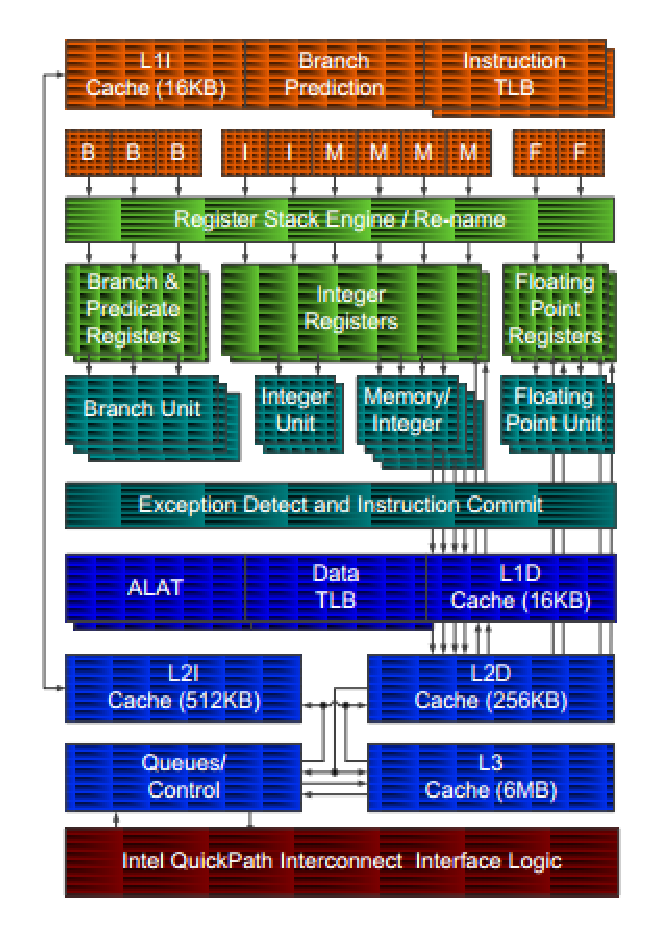
\includegraphics[height=5cm,
    angle=0]{./images/Intel_Itanium_Tukwila_core.eps}}
  \caption{Intel Itanium Tukwila CPU core}
  \label{fig:Intel_Itanium_Tukwila_core}
\end{figure}

With many more number of cores in GPU than in CPU, the GPU cores are much
simpler and smaller. A major fraction of GPU is occupied by the transistors
(higher density than that in CPU), i.e. CPU run a lot hotter than the average
CPU, especially when playing games.

  
Both Nvidia and ATI's AMD manufacture GPUs with a slightly difference in
hardware design
\begin{itemize}
  \item Nvidia GPU: fewer cores but the cores are capable of more complex tasks
  than AMD cores
  
  \item AMD GPU: more cores that can significantly speedup the calculations
  (but less flexible)
\end{itemize}


In terms of speed (Sect.\ref{sec:clock-cycles-speeds}),  ATI's SP is different
from Nvidia's SP (CUDA core): ATI's SP run at core speed, while Nvidia's SP  run
well beyond core speed. ATI's SP can't do texture and shading at the same time;
while Nvidia's SP can. In recent CUDA architecture, all Nvidia CUDA core are
identical (unified); while some of ATI's core are missing some capabilities,
e.g. one out of every 4 ATI's core is missing the dot-product hardwares. To make
it easier, we will focus on the comparison between Intel CPU core and Nvidia GPU
cores (if not mention explicitly).
  
\begin{framed}
  When comparing CPU core vs. GPU core, we look into 
  \begin{enumerate}
    \item CPU complete: more complicated, with cache, registers. In GPU,
    cache only available at streaming multiprocessor (SM) level from 2nd
    generation. Also, registers are not part of GPU core.
    \item instruction set: CPU core can handle complicated operations, but CPU
    core only does simple arrhithmetic operation, and a separate special
    functional unit is required to do complicated operations like square-root,
    exponential function.
  \end{enumerate}
\end{framed}
  
Cores\footnote{\url{http://en.wikipedia.org/wiki/Multi-core_processor}}:
 
  \begin{itemize}
  \item CPU: Intel Nehalem (2,4,6,8,10, 12), AMD Opteron
    (1,2,4,6,8,12), UltraSPARC T2 ({\it codename: Niagra 2}) (8 CPU cores),
    UltraSPARC T3 (16 CPU cores).
    
    NOTE: Intel's Tera-scale Research Program introduced many-core CPU Polaris
    (80-core processor in 2007) with cores here are simpler than CPU cores used
    in multi-core CPUs. Each core has 2 floating-point engines.
    
    IntellaSys introduced SEAforth 40C18 (40-core processor) embeded processor
    in 2008. Each core is a complete computer with
    its own RAM and ROM (64-word each) and can operate asynchronously with other
    cores
    \footnote{\url{http://dbaspot.com/arch/419828-intellasys-seaforth-40c18-40-core-processor-guy-macon.html}}.
    To program on it, we use  VentureForth, a Forth-based IDE in both Windows and Linux.
    
\begin{framed}
  Until May, 2010, the fastest CPU chip of Intel,
  {\it codename ``Knights Ferry''}, has 32 CPU cores and is being used
  for development purpose. The first commercial product will
  include more than 50 cores and to be called ``Knights Corner''
  (Sect.\ref{sec:Intel_GPGPU}).
\end{framed}
    
  \item GPU G80 (e.g. GeForce 8800 GTX) - Nov, 2006: the first generation of
  Tesla architecture GPU, with 128 CUDA cores (shaders), use 90nm technology
  (Sect.\ref{sec:g80g92-architecture}). G80 has 690M transistors.
  
   
  \item[*] Tesla 1st gen (chip G80, no VGA/DVI output) - C870
  
  \item GPU G92 (e.g. GeForce 8800 GT): use 65nm technology, with 754M
  transistors.
  
  \item GPU GT200 (e.g. GeForce GTX 280): the second generation of Tesla
  architecture that uses 65nm (GT200A) and 55nm (GT200B), with 240 cores and
  1.4B transistors.
  
  NOTE: GT = Graphics Tesla, GF = Graphics Fermi, GK =  Graphics Kepler
  
  \item [*]Tesla 2nd gen (chip GT200a/b, no VGA/DVI output) -
    C1060/S1070
    \item [NOTE] Project G200b/GTX285 use 55nm technology
    \item [NOTE] Project G212/G214 failed to use 45nm technology
    
  \item GPU GF100 - theory 512 cores, yet due to 40nm architecture
    restrictions, some of them are disabled (e.g. GeForce GTX 480 has
    480 cores, GeForce GTX 470 has 448 cores). 
    
  \item [*] Tesla 3rd gen (codename: {\it Fermi}): C2050/C2070 with 512 cores
  grouped into 16 SMs.
  \item [*] chip GTX 470, with DVI output - use GF100; GTX 475 use GF104.
  \item 
    \textcolor{blue}{GPU GF104/GF106/GF108: a remake of
      GF100 by making a smaller verion of Fermi architecture rather than taking
      larger GPU. So, they have less cores, less
      memory, lower bandwidth} (Jul, 2010). 
      
      \item [*] GTX 460, GTS 455 use GF104 with 336 cores, 675MHz graphics clock
      (i.e. 1350 processor clock) and 1GB 1.8GHz memory. GTS 455 is, however,
      slower than GTX 460.
%      \item [*] GTX

   \item GPU GK110 - uses 28nm technology features 1024 CUDA cores, with 7.1 billion transistors.
   
    
   \item [*] Tesla 4th gen (codename: {\it Kepler}): use GK110 
   
   \item \textcolor{blue}{GPU GK100/GK102/: lower level of GK110 targetting to
   computer graphics}. GeForce GTX 680 has 10.0'' long; GeForce GTX 690 has
   11.0'' long while GeForce GTX Titan is 10.5'' long (AMD Radeon HD 7970 is
   11.5'' long).
   
   \item Tesla Maxwell GM200 uses 28-nm FFN with 8 billion transistors.
   
   \item Tesla P100 GPU - uses 16nm FinFET, with 15.3 billion transistor GPU
   
   \item  GV100 GPU - use new TSMC 12 nm FFN (FinFET NVIDIA) with 21.1 billion transistors with a die size of 815 mm$^2$.
  
  
  \end{itemize}


\begin{figure}[hbt]
  \centerline{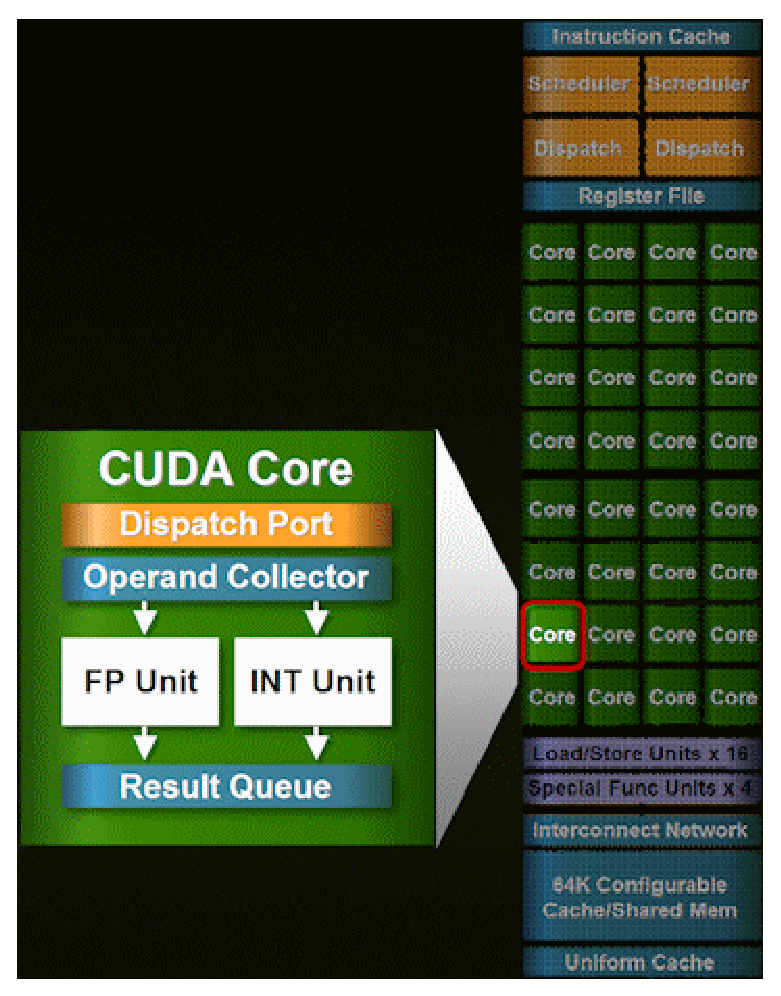
\includegraphics[height=7cm,
    angle=0]{./images/gpu_core.eps},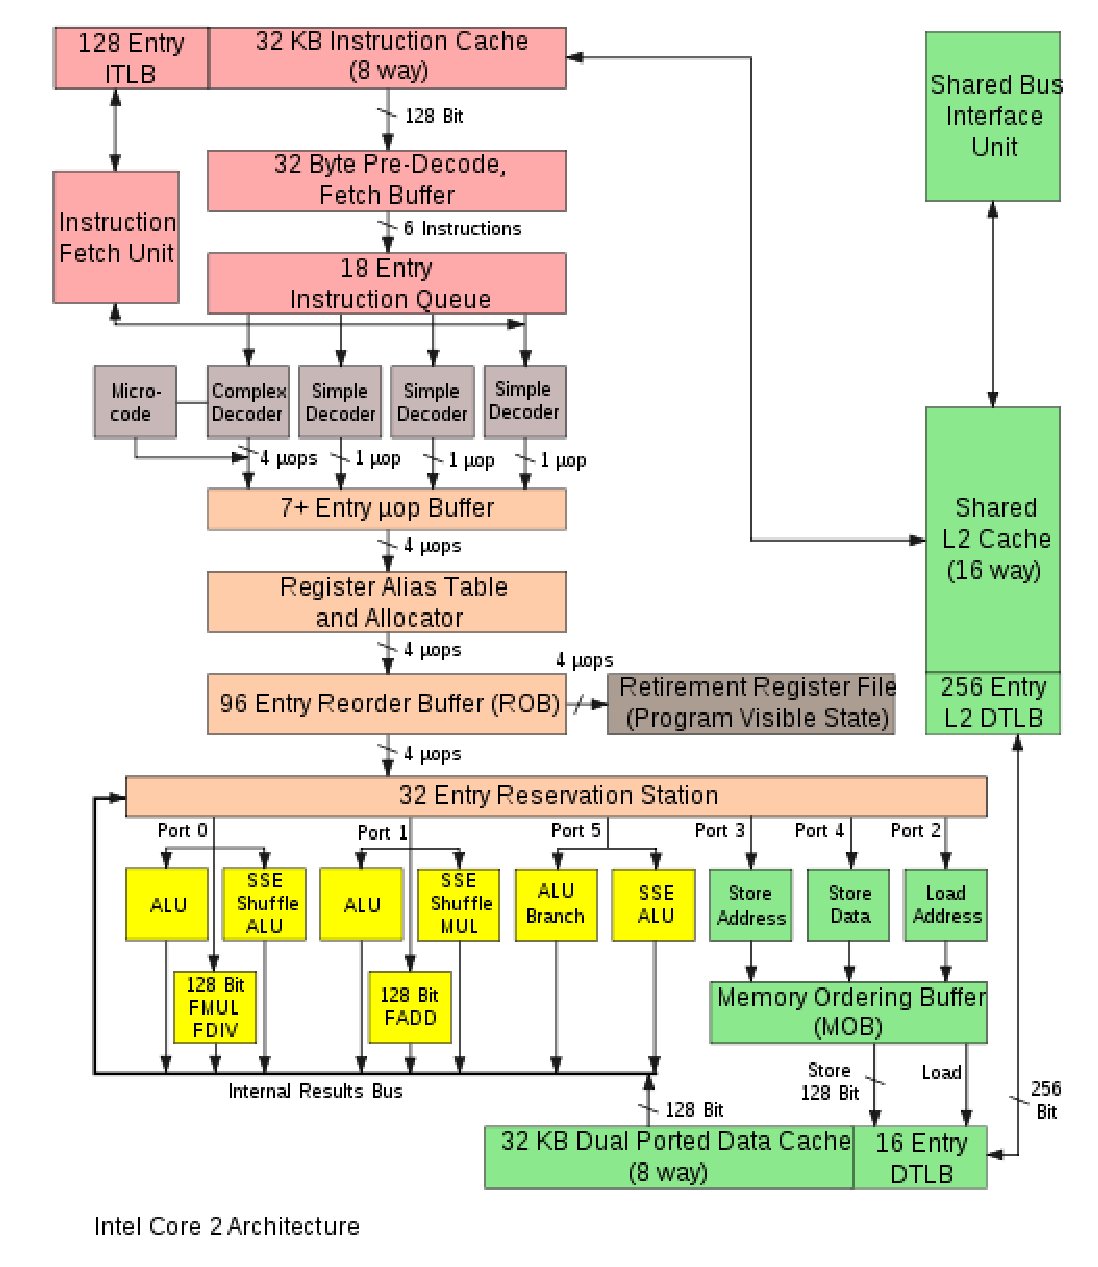
\includegraphics[height=7cm,
    angle=0]{./images/core2_intel.eps}}
 \caption{(A) GTX280 GPU core, (B) Intel Core2
 \footnote{\url{http://blog.langly.org/2009/11/17/gpu-vs-cpu-cores/}}}
\label{fig:gpu.cpu_core}
\end{figure}

A CPU core can execute four 32-bit instruction per clock (using 128-bit SSE) or
eight 32-bit instructions (using AVX 256-bit registers). A GPU like Radeon HD
5970 can execute 32000 32-bit instructions per clock (using 32000 ALUs or
shaders). Even a typical multi-core CPU has more core (upto 6, 8 or 12) and
higher frequency clock (2000-3000 MHz vs. 735MHz in Radeon HD 5970), a Radeon
GPU still runs more than 5x faster, yet with a cheaper cost (350\$ vs. a
12-core CPU 4700\$). Recently, Intel have introduced a GPU-like platform called
Xeon Phi, with 86 cores that can deliver 1 TFLOPS double-precision.

References:
\begin{itemize}
\item \url{http://blog.langly.org/2009/11/17/gpu-vs-cpu-cores/}
\end{itemize}



\section{Memory hierarchy in GPU}

\subsection{Register files}
\label{sec:register-files}

A {\bf register} (or register file) refers to the kind of storage with smallest
access latency (extremely fast memory space, with access time is almost zero).
Accessing data in registers just take a few bits of encoding - unlike memory
address, where we need a longer address to refer to a variable.
Small access latency means an expensive in hardware implementation; thus the
number of available registers in CPUs are very small (read Chapter {\it X86 and
X86-64} in Fortran book).


GPGPU has been designed with a large number of register files. The goal is
minimize the latency in thread switching, i.e. lightweight thread. This is not
the case in CPU, i.e. heavy-weight thread, as each thread switching requires
backing up the data in the register files (Sect.\ref{sec:threads-1}).

Early GPU has register file of 32-bit. Recent GPUs has register file of
64-bit (Fermi GPU).  CPU registers are more complex with 128-bit, and
recently 256-bit.
% 
% However, the memory space is limited. The memory is splitted into a number
% of 32-bit or 64-bit register file, depending on architectures. 
  \begin{itemize}
  \item CPUs: dozens of registers, e.g. SPARCS v8 has 160
    general-purpose registers (yet only 32 are available to software =
    8 global registers + 24 forms register window, each window has 8
    local
    registers\footnote{local registers are used for retaining local
      values across function calls}
    and shares 8 registers with adjacent
    windows\footnote{the shared registers are used for passing
      function parameters and returning values}),
    16 64-bit
    registers\footnote{can be used as 32 single-precision registers or
      8 quad-precision registers}.
      
  \item Nvidia C870: 8192 32-bit registers
\item Nvidia Tesla C1060: 16384 32-bit registers
\item Nvidia Fermi C2050: 32768 32-bit registers
%\item AMD Cypress has 16384 128-bit registers
  \end{itemize}

% The maximum number of registers per SM (streaming multiprocessor) is
% \begin{itemize}
% \item 8192 in Tesla 1st gen (CC.1.0, CC.1.1)
% \item 16384 in Tesla 2nd gen (CC.1.2,CC.1.3)
% \item 32768 in Tesla 3rd gen (CC.2.0)
% \end{itemize}

For more information, read Sect.\ref{sec:register-memory} and
Sect.\ref{sec:registers-ptx}.


\subsection{Constant, Shared and Cache memory}
\label{sec:const-shar-cache}

Constant, shared and cache memory are fast access memory, yet slower than
Register file memory (Sect.\ref{sec:register-files}). Shared and cache are
on-chip memory, while constant memory reside on global device memory
(Sect.\ref{sec:constant-memory}, yet the mechanism for reading data from
constant memory allows the data to be cached in a cache-memory making it can be
accessed faster from the second read access.
% Amount of Constant, Shared and Cache Memory
  \begin{framed}
    A cache is a smaller, faster memory which stores copies of the
    data from the main memory location (RAM). Two main caches are
    {\bf instruction cache} (speed up instruction fetch) and
    {\bf data cache} (speed up data fetch and store). 
    \begin{itemize}
    \item CPU often have
      large cache to reduce the latency in data fetching, thus maximize
      performance of the sequential-execution model. 

    \item GPU, however, is designed to do multiple computation at the same
      time. Thus the hardware for execution units (arithmetic execution)
      take a large portion of the chip. As a result, GPU has a restricted
      amount of shared and cache memory. 
    \end{itemize}
    As off-chip memory access is high-latency, it's recommended to
    maximize using on-chip memory (constant, shared memory, cache) by
    having algorithms of high locality of memory access (to be
    discussed later).
  \end{framed}

Cache can be classified into L1, L2, and L3 cache. The lower the number the
faster memory access. In a multicore CPU architecture, L1 cache is accessible
for a single core, L3 is shared by all cores, and L2 is intermediate between L1
and L3 yet accessible by a single core (NOTE: access time $L1<L2<L3<$RAM).

\begin{mdframed}

Old CPUs has L1 cache and SRAM as L2 cache. In newer CPUs, L2 is moved into CPU,
i.e. both L1 and L2 on CPU, and they added L3 cache. Multicore CPU has L3 moved
to CPU as well, yet is shared by multicore in a single CPU, while L1 and L2 are
dedicated to a single core (except Intel Core 2 has 1MB-6MB L2 cache shared by 2
CPU cores and use this to communicate between 2 cores). Size: L1 cache (16-64KB
per core, for each instruction cache and data cache), L2 cache (256KB-1MB per
core, hold both  instruction and data).

Latency in x86 CPUs: L1 cache (2-3 clock cycles), L2 cache (10-12 clock cycles),
L3 cache (dozens of clock
cycles)\footnote{\url{http://www.tomshardware.com/forum/297190-28-about-cache}}.
\end{mdframed}

\subsection{Texture memory}

Unlike CPU where LD/ST units are an integral part of the CPU core, texturing and
render output are decoupled from the CUDA core, Fig.\ref{fig:GT200_texture}.
Here, the SM controller can read data either from the texture data (which can
be from L1 texture cache, L2 texture cache or global memory), general data
from the global memory; then process and save it to the global memory (in the
case of a graphics application, the result is passed to Raster Engine (ROP)).
So, what is texture memory? As shown in Fig.\ref{fig:GT200_texture}, there are
two specialized texture caches.

Memory in CPU RAM, CPU caches have locality in a single dimension because memory
addressing for most architectures is linear. Typically, data is fetched in
groups, defined by the {\bf cache line}. An example from Intel Itanium Tukwila
is given in Fig.\ref{fig:Intel_Itanium_Tukwila_cacheline}. Here, L1 cache is
4-way, L2 cache is 8-way and L3 cache is 12-way.
% If the data cache and
% instruction cache are separated.

\begin{figure}[hbt]
  \centerline{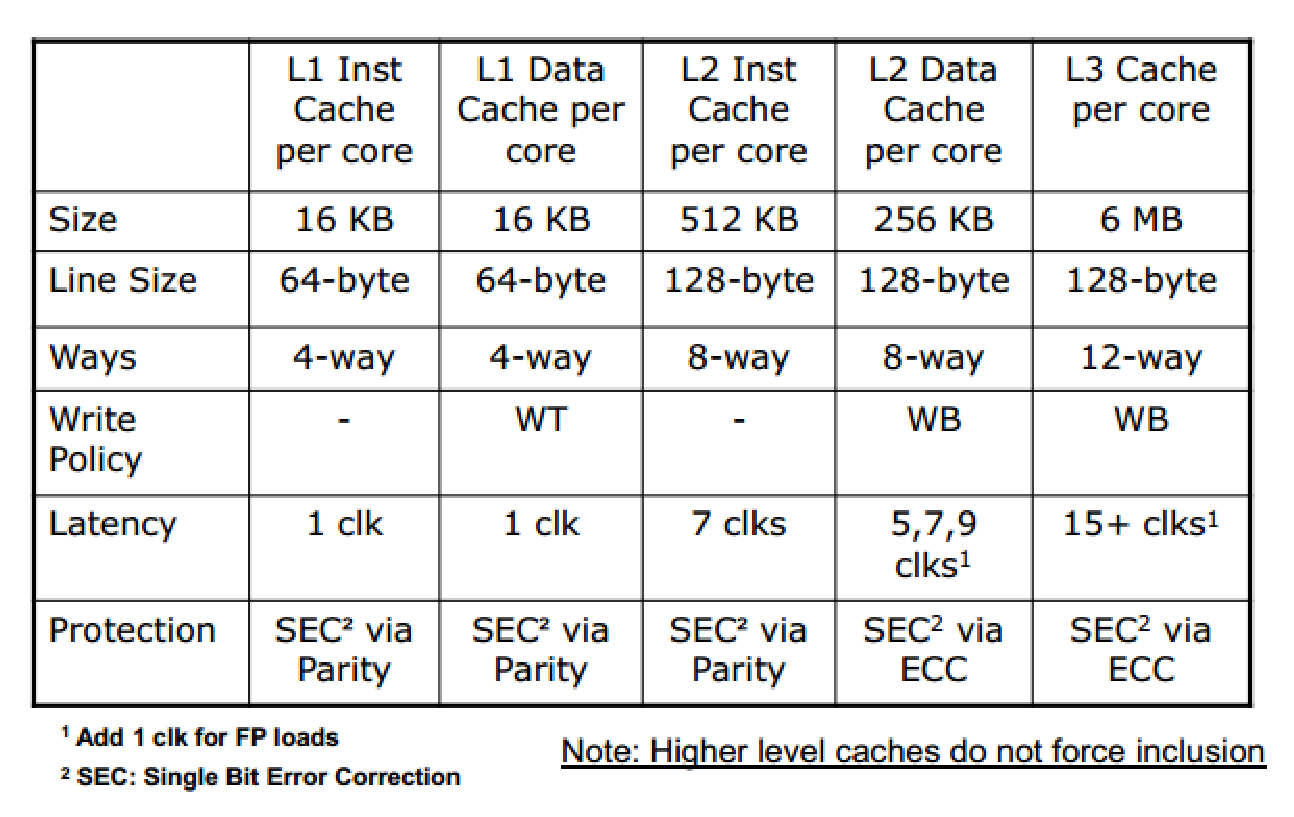
\includegraphics[height=5cm,
    angle=0]{./images/Intel_Itanium_Tukwila_cacheline.eps}}
  \caption{Cache line in Intel Itanium Tukwila CPU}
  \label{fig:Intel_Itanium_Tukwila_cacheline}
\end{figure}

\begin{mdframed}

Caches come in different forms and capacities. But now matter how large or small
they are, caches fall into one of the three categories: {\it direct mapped},
{\it n-way set associative}, and {\it fully associative},
Fig.\ref{fig:Cache_structures}. Depending which one is being used, a cache block
is identified using upto three information: tag, index, and offset. If a cache
slot is small enough to put one cache block, then it's direct mapped, and make
it easier to find the block, but it's not flexible about where to put the
blocks. In {\it n-way associative}, we have, example 2-way or 4-way associative
cache. In 2-way set, we can put two cache blocks in a slot or in 8-way set, we
can put a cache block in one of 8 different locations, i.e. giving some
flexibility.

The index is used to find the slot index, and the tag is used to find the block
within the set of cache blocks inside the slot. \textcolor{red}{The hardware is
very complicated with fully associative caches (as it requires parallel searchs
of all slots)}
\footnote{\url{http://csillustrated.berkeley.edu/PDFs/handouts/cache-3-associativity-handout.pdf}}
\end{mdframed}

\begin{figure}[hbt]
  \centerline{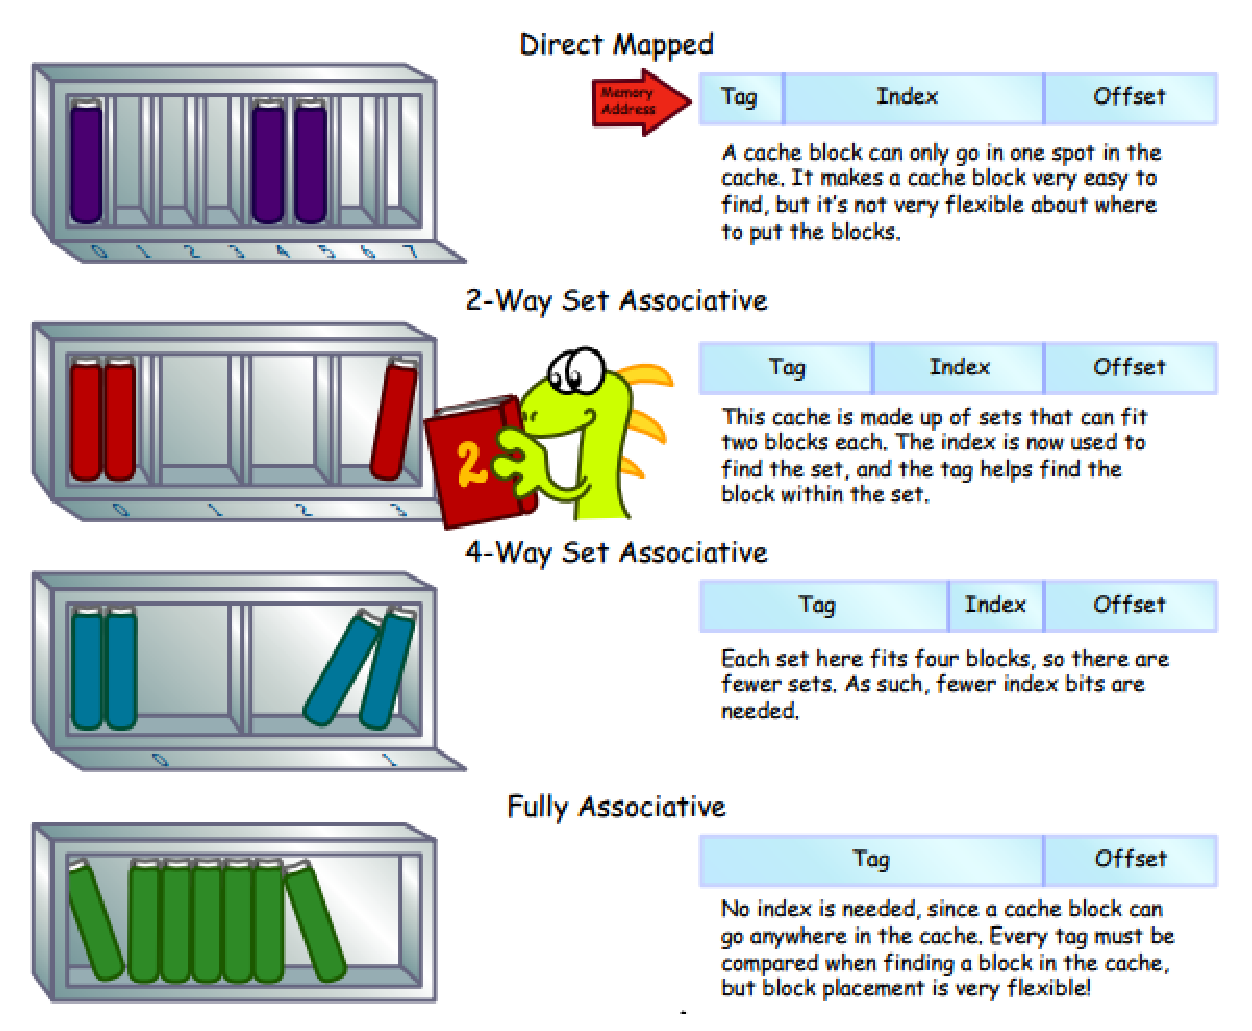
\includegraphics[height=5cm,
    angle=0]{./images/Cache_structures.eps}}
  \caption{A cache is like a bookshelf: how we divide the slot to put one or
  more books in each slot}
  \label{fig:Cache_structures}
\end{figure}


Suppose the cache line is 64-Byte, a
read of one data word (4Byte or 8Byte) results 64-Byte to be read. Most of the
time, the unused 56B-60B of data are in closed proximity to the original
requested data. GPU global memory are physically organized in a similar linear
layout (i.e. 2D or 3D data structures are ultimately mapped to 1D).

However, GPU has a special memory space that is designed to work with 2D data
(and recently with 3D data) that random access to any item in the array A[i,j]
take the same amount of time - known as {\bf texture memory}.
\textcolor{blue}{Texture memory in C1060 is specifically designed for optimal 2D
pixel/voxel-based memory access in graphical applications. Texture memory in
Fermi GF100 support both 2D and 3D pixel/voxel-based memory access}. NOTE:

\begin{enumerate}
  \item  texture caches are read-only and have no coherency. When a texture is written,
the entire texture cache hierarchy must be invalidated, rather than tracking the
validity of individual data within the address space. 
  \item unlike CPU cache that lowering latency (from 100ns to 7ns), GPU texture
  cache is used to avoid bandwidth and power consumption. 
\end{enumerate}

\begin{figure}[hbt]
  \centerline{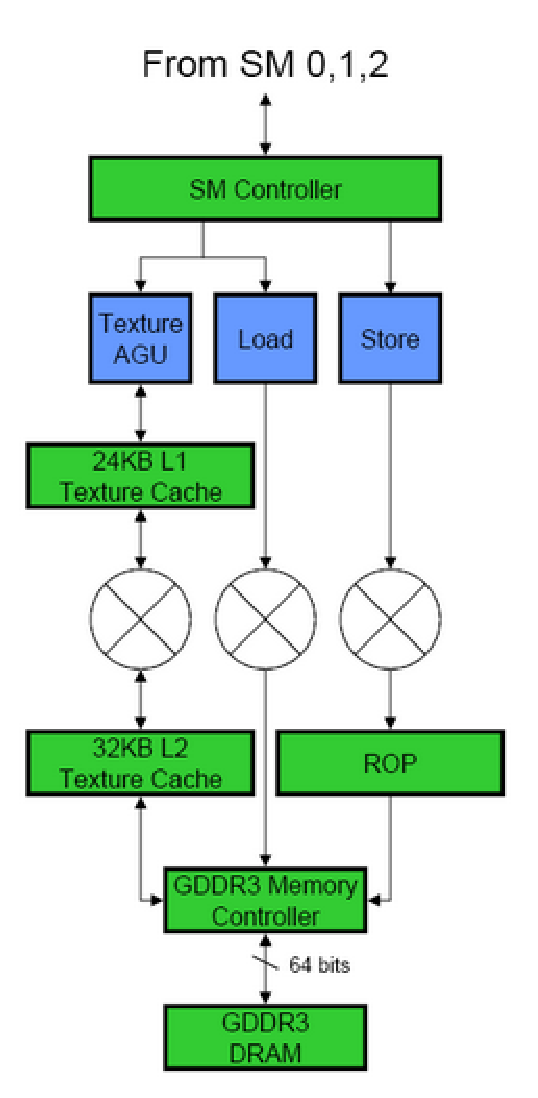
\includegraphics[height=5cm,
    angle=0]{./images/GT200_texture.eps}}
  \caption{Texture Unit, ROP and Memory Pipeline}
  \label{fig:GT200_texture}
\end{figure}


As texture-cache are designed for graphical applications, and access this memory
require using Texture CUDA Graphical APIs, it's not popularly used by a
general scientific high performance computing application.

  \begin{itemize}
  \item CPU: use large caches to convert long latency memory access to
    short cache sequential accesses,
    Fig.\ref{fig:Intel_Itanium_Tukwila_cacheline}. It thus uses sophisticated
    control to improve sequential execution.
    \begin{itemize}
    \item Intel Nehalem (32KB L1 instruction + 32KB L1 data (L1D)
      cache memory per core; 256KB L2 cache memory, 4-8MB L3 cache
      memory),
    \item AMD Opteron (64KB L1 instruction + 64KB L1D cache each core;
      1024KB L2 cache (single core), 2*1024 (dual-core), 512KB per
      core (quad-core); 1024KB L3 (quad-core Barcelona), 6MB L3 each
      core (quad-core Istanbul + Shanghai), 2*6MB L3 shared (8-12
      core))\footnote{\url{http://en.wikipedia.org/wiki/Opteron}}.
    \item Niagra 2 has 8KB L1D cache per CPU core. Totally, the chip
      has 4MB L2 cache with 8 banks.
    \end{itemize}
  \end{itemize}
  GPU uses small caches; which can be accesses in parallel. So, it
  boosts memory throughput via many, long latency but heavily
  pipelined caches.

  \begin{itemize}
  \item Tesla 1st gen C870 (per cluster = TPC = 2 SMs; 1 SM = 8 SPs):
    8KB read-only {\it constant-cache memory} (or just constant
    memory), 16KB L1 read-only texture cache (texture cache are
    originally designed for graphical applications). Totally, with 8
    clusters, a GPU has $8\times 8=64$KB constant-cache memory, and
    $16\times 8=128$KB L1 texture cache.

    The whole-chip L2 texture cache is also 128KB and is divided into
    6 banks.

    Per SM, it has 16KB shared memory (i.e. $8\times 2\times 16=256$KB
    shared-memory totally).

  \item Tesla 2nd gen C1060 (per cluster = TPC = 3 SMs; 1 SM = 8 SPs):
    6.4KB read-only constant memory; 24KB L1 read-only texture
    cache (partitioned into 3x8KB). Totally, with 10 clusters, a GPU has
    $6.4\times 10=64$KB constant memory and 10 x 24KB = 240KB L1 texture cache.

    The 256KB L2 texture cache is shared by all TPC and is divided
    into 8 banks, i.e. each bank is 32KB.

    Per SM, it has 24KB shared memory (i.e. $10\times 3\times
    24=720$KB). 

    \begin{framed}
      Only Fermi has true L1/L2 cache.  C870 and C1060 indeed have
      L1/L2 {\bf texture cache} which are originally designed to work
      with pixel/voxel-liked data. Texture caches were mostly useless
      when GPU run in compute mode (high-performance scientific
      applications); however, it's possible to use it if we can manage
      carefully using Texture CUDA API.
      \textcolor{red}{CUDA Fortran 2010 has not been implemented the
        API to process data from texture cache yet}. Texture memory is supported 
        in CUDA Fortran 2013 (Sect.\ref{sec:cudafortran_texture}).
    \end{framed}

  \item Fermi C2050/C2070 (per cluster = GPC = 4 SMs; 1SM = 32 SPs):
    4KB read-only constant memory. Totally, with 16 clusters, a GPU
    has 64KB constant memory. A GF100 GPU has 4 (GPC) x 4 (SM/GPC) x 12
    (KB/SM)=192 KB L1 texture cache. 

    The chip has total 768KB L2 cache shared equally by all SMs,
    i.e. maximum 48KB per SM in C2050.

    Per SM, it has 64KB configurable on-chip memory (48/16 or 16/48
    configurable for shared/L1 cache) which is managed by the compiler
    (sect.~\ref{sec:shared-memory-cache}).
  \end{itemize}

\subsection{Off-chip memory}
\label{sec:chip-memory}

Off-chip memory are aka global device memory (RAM). The speed of RAM is
determined by different factors, e.g. dual channel. The maximum theoretical
bandwidth (burst rate) is given as an example below
\begin{verbatim}
   RAM_base_clock_frequency x 
x  num_data_transfer_per_clock (which is 2 for DDR/DDR2/DDR3)
   memory_bus_width 
   num_interfaces   
\end{verbatim}

Example: 933 MHz, memory bus 64-bit
\begin{verbatim}
 (933 million hertz * (2 interfaces) * (64 lines/interface) * 
 (2 bits/line-cycle)) = 238,848 Mbit/s, or 29,856 MB/s, or 29.15 GB/s. 
\end{verbatim}
\url{http://en.wikipedia.org/wiki/Memory_bandwidth}

We will discuss different technologies
\begin{enumerate}
  \item GDDR3 - Sect.\ref{sec:GDDR3}
  \item GDDR5 - Sect.\ref{sec:GDDR5}
  \item HBM2 - Sect.\ref{sec:HBM2-RAM}
\end{enumerate}

\subsection{-- GDDR3, GDDR4}
\label{sec:GDDR3}

The RAM in motherboard (CPU) is DDR, while the RAM on CPU is GDDR.
The technology is the same (double-data rate), yet the specifications are
different. GDDR can run at a higher speed while using a smaller voltage. 

GDDR3 is an open standard developed by ATI in conjunction with the standards
organization JEDEC Solid State Technology Association. ATI and Nvidia both work
on to develop GDDR4; but only ATI use it. GDDR4 main improvement is using 1.5
Volts instead of 1.8 Volts (however at higher clock rates, it still need 1.8
Volts for stability). Another improvements: (1) prefetch scheme use 8bits, (2)
burst length is locked at 8 bits (defined data sent in burst mode, i.e. the
mode in which data are being sent without waiting for input from another
device). GDDR5 only requires 1.5 volts, with density ranging from 512Mb to 2Gb
modudles (i.e. four 2Gb modules form 1GB frame buffer). GDDR5, theoretically can
deliver twice the memory bandwidth of GDDR3 at the same clock frequency.
 
GDDR3 improved on previous GDDR designs by supporting higher clock speeds while
requiring less power. These chips consume less electricity, so they produce less
heat and can rely on simpler cooling hardware (GDDR3's VDD and VDDQ voltage
requirements are both 1.8 volts). GDDR3 also has separate read and write data
strobes, which contributes to a much faster read-to-write ratio (meaning the
turnaround from a read operation to a write operation occurs much more quickly)
than GDDR2 supported. GDDR3 chips have a hardware reset feature that can wipe
their memory clean to start receiving new data should such an operation be
necessary.
\footnote{\url{http://www.maximumpc.com/article/features/everything_you_need_know_about_gddr_memory}}

Amount of off-chip memory

\begin{itemize}
  \item CPU: max 4GB (32-bit OS), max $2^{14}\times 4$GB (48-bit), max
    $2^{32}\times 4$ GB RAM (64-bit)

  \item Tesla 1st gen C870: 1.5GB GDDR3

  \item Tesla 2nd gen C1060: 4GB GDDR3
\end{itemize}

Off-chip memory throughput (theory), as shown inFig.~\ref{fig:tesla_singlenode}

\begin{itemize}
  \item CPU access RAM DDR-400 : 3.2GB/sec
  \item C870 access device memory DDR3: 76.8 GB/sec
  \item D870 ... : 153.6 GB/sec
  \item S870 ... : 307.2 GB/sec
  \item C1060 access device memory DDR3: 102 GB/sec (4GB board)

    \begin{framed}
      NOTE:
      \begin{itemize}
      \item  140 GB/sec (1GB boards, e.g. GTX285)
      \item GDDR5 is DDR3-based graphics memory.
      \end{itemize}

    \end{framed}
  \item S1070 ... : 409 GB/sec
\end{itemize}

\subsection{-- GDDR5}
\label{sec:GDDR5}

GDDR5 is based on DDR3 (since 2008), Fig.\ref{fig:GDDR_mem}. GDDR5 equals
176Gb/sec, DDR3 equals 68Gb/sec (Sect.\ref{sec:GDDR3}).
However, GDDR5 has a slighter higher latency. This latency can be hidden by
well-written code on CPU; and on GPU by the pipeline
works.\footnote{\url{http://www.ign.com/blogs/sonyhaswon/2013/06/22/gddr-5-vs-ddr-3-the-full-breakdown}}

\begin{figure}[hbt]
  \centerline{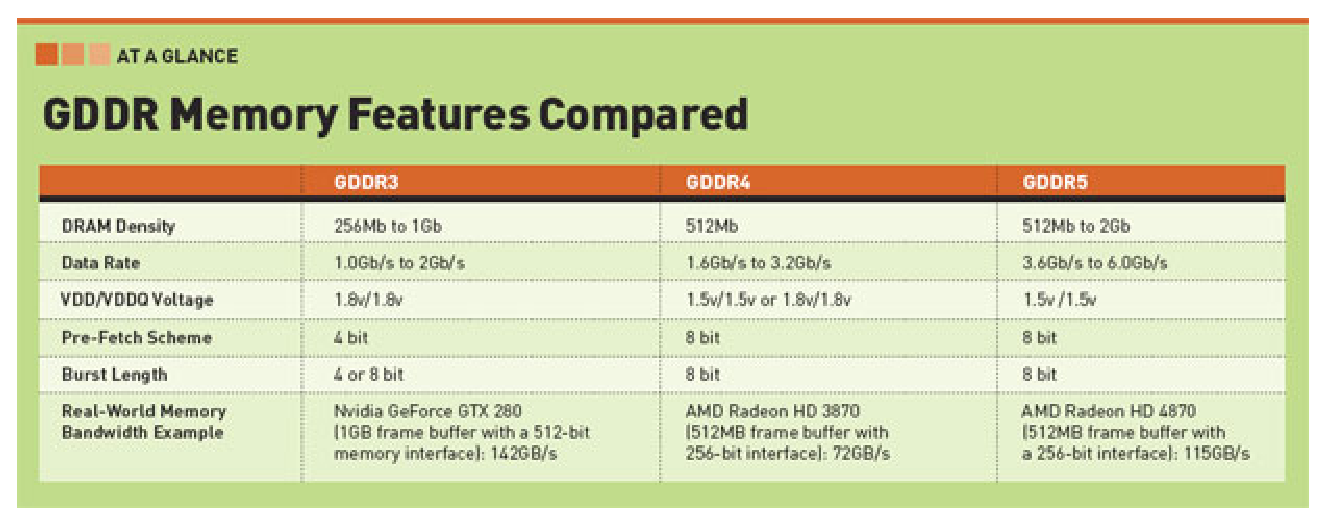
\includegraphics[height=5cm,
    angle=0]{./images/GDDR_mem.eps}}
  \caption{GDDR memory at a glance}
  \label{fig:GDDR_mem}
\end{figure}


Amount of off-chip memory
  \begin{itemize}

  \item Fermi: C2050 has 3GB GDDR5, C2070 has 6GB GDDR5 [NOTE: If
    ECC\footnote{ECC=error correction code, a technique to detect
      error during the storage and transmission of data}
    is enabled, a portion of memory is removed from your usage (12.5\%
    of memory is reserved for ECC checking, so C2050 has only 2.625GB with ECC
    enabled;) and GPU runs a little bit slower.]
  \end{itemize}

  \begin{figure}[hbt]
    \centerline{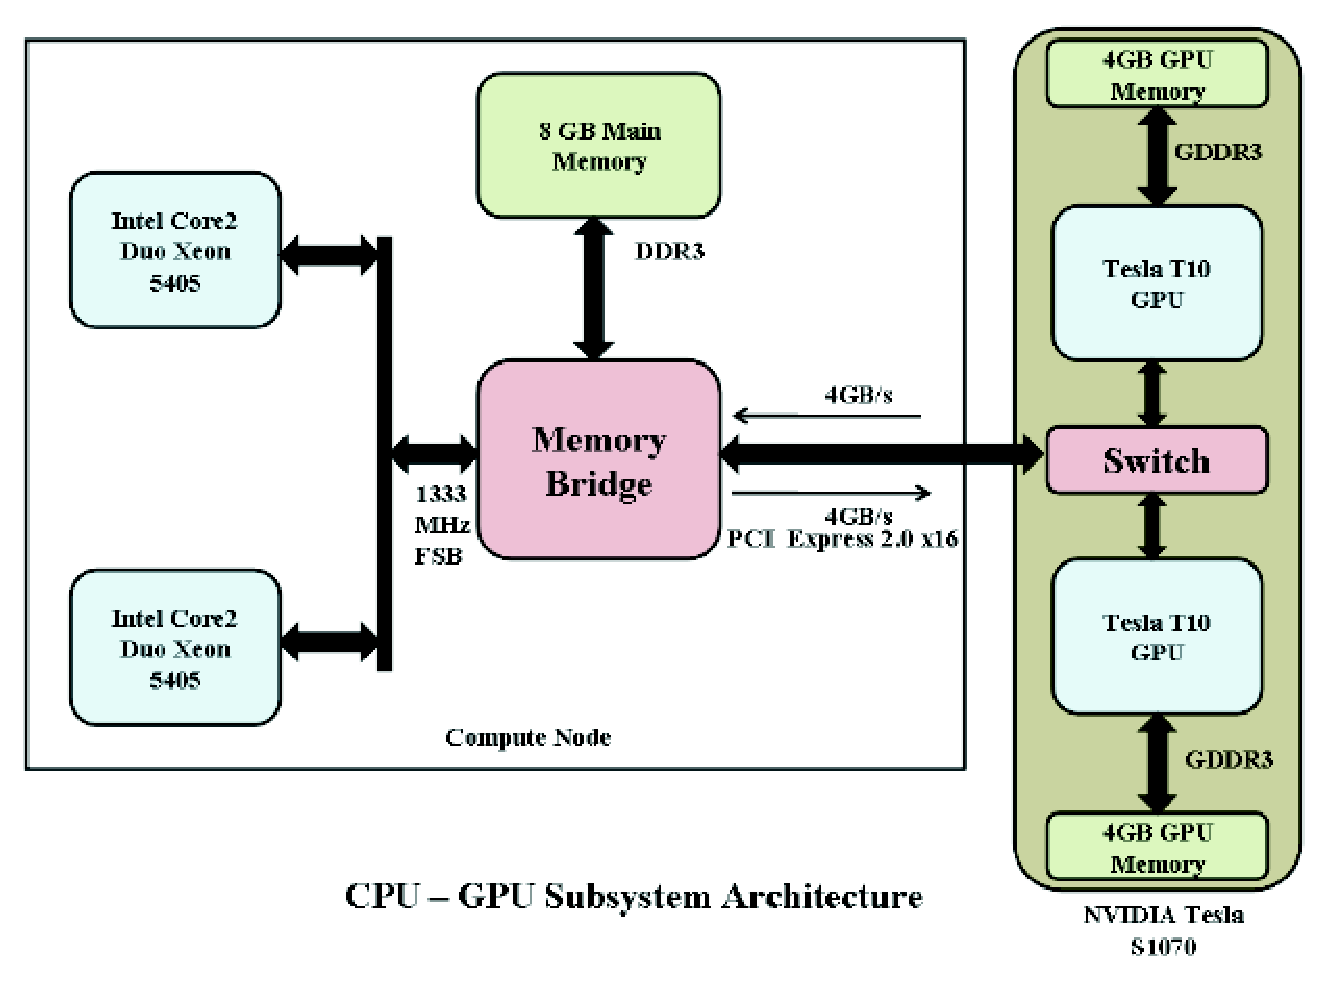
\includegraphics[height=7cm,
      angle=0]{./images/tesla_connect.eps}}
    \caption{Memory access speed: 2 separate dual-core access, each
      compute node access to two Tesla T10 GPU (4 T10 GPUs are packed
      in Tesla S1070)}
    \label{fig:tesla_singlenode}
  \end{figure}

Off-chip memory throughput (theory), as shown in
  Fig.~\ref{fig:tesla_singlenode}
\begin{itemize}

  \item C2050/C2070 access device memory GDDR5: 1152 Gbps = 144 GB/sec (planned
  230 GB/sec, but not able to reach)

  \item
    \textcolor{blue}{M2050/M2070: is C2050/C2070 with an increased in
      memory bandwidth (148 GB/sec)}\footnote{\url{http://www.Nvidia.com/object/product_tesla_M2050_M2070_us.html}}
   
   \item S2050/S2070 ... : $4\times 148=593$ GB/sec
     
  \end{itemize}
  
This value is dependent upon the memory bus bandwidth, the number of memory controller per chip, etc.
  
\subsection{-- HBM2}

Check Sect.\ref{sec:HBM2-RAM}.


\section{Memory Addressing}
 
 In G80 GPUs, an address is defined using 32-bit virtual addressing. To know the
 real address, memory instructions use register plus offset addressing. This
 virtual address is translated into the real address by the MMU.
  
 In GT200 GPUs, an address is defined using 40-bit virtual addressing.
 
 In GF100 GPUs, \ldots
 
 The NVIDIA Fermi GPU architecture, introduced in 2009, implemented a unified GPU address space
spanning the three main GPU memory spaces (thread private local memory, thread block shared
memory, and global memory). This unified address space only applied to GPU memory addressing, and
mainly resulted in simpler compilation by enabling a single load/store instruction and pointer address to
access any of the GPU memory spaces (global, local, or shared memory), rather than different
instructions and pointers for each. This also enabled full C and C++ pointer support, which was a
significant advancement at the time

 
 \subsection{Load/Store}
 
 In order to efficiently access memory, loads and stores must be aligned to
 4Byte boundaries - improperly aligned accesses will result in multiple loads
 or stores being generated by the compiler.  Load instructions across different threads in
a half-warp can be coalesced by the memory controller to reduce the number of
memory transactions.
 
 
 \subsection{Bandwidth information}
 
  \textcolor{red}{We'll describe how to compute the bandwidths from
    these values in Sect.~\ref{sec:hardware-information}}. In 
    \begin{itemize}
      \item GTX 460: 115.2 GBps (256-bit, 1800 MHz)
      \item GTX 460 v2: 96.2 GBps (192-bit, 2004 MHz)
      \item Tesla C2050/C2070: GPU-GDDR5 144 GBps
      \url{http://www.nvidia.com/docs/IO/43395/NV_DS_Tesla_C2050_C2070_jul10_lores.pdf}
      \item GTX 770: 224.3 GB/s (, 7.0 Gbps)
      \url{http://www.nvidia.com/gtx-700-graphics-cards/gtx-770/}
      \item GTX Titan: 288.4 GB/s (384-bit, 6.0 Gbps)
    \end{itemize} 
The number depends on memory clock frequency (i.e. 2 GHz or 7.0 Gbps), memory
interface width (i.e. 256-bit or 512-bit).
    
    
    The major botle-neck is the bandwidth between GPU-DDR3 (dual direction on PCI-e Gen2 x16, DDR3 =
    CPU RAM): 64 Gbps (i.e. 4 Gbps for each direction) [NOTE:
    64Gbps=8GB/sec]. Bandwidth between CPU-DDR3 is about 256 Gbps = 32 GB/sec.
    The connection between CPU-CPU using Intel QuickPath Interconnect (QPI) is
    about 102 Gbps = 12.75 GB/sec. 
    
    Reading and writing data to harddrive is even
    slower:    CPU-SAS/SATA controller is carried out via PCI-e Gen2 x4 = 32 Gbps; and
    SAS/SATA controller - Local Disk is about 8.4 Gbps. On network using
    Infiniband, CPU-Infiniband using PCI-e Gen2 x8 is about 32 Gbps. If we use
    dual Infiniband card per node, the speed would be 2x32=64 Gbps. 

  \begin{framed}
    Due to the low data transfer speed between CPU-GPU, you should
    minimize copying data back and forth. If you need to copy the
    data back to do some computation on CPU, it's sometime better to
    do that directly on GPU to avoid copy data back, even though
    running on GPU is slower than running on CPU.

    If you need to copy the data, it's better to copy a single large
    size batch of data, rather than many small size chunks.
    \textcolor{red}{The recommended size is a chunk not larger than 10MB, and a
    multiple of 64}. Larger than that, we observe a saturation in performance.

    If not overwritten, data on off-chip memory and L2 cache are preserved
    between kernel calls.
  \end{framed}

At SC14, a team of researchers from Argonne National Laboratory and DataDirect
Networks (DDN) moved 64 TB of data in under just 100 minutes using 100 Gbps WAN
connection, i.e. about 16 hours using 10 Gbps. This typically takes 2 days using
10 Gbps connection. They were abled to sustain data transfer rates over 85 Gbps,
with peak at over 90 Gbps (benchmarked using \verb!iperf! tool). They used
\begin{itemize}
  \item Globus GridFTP server
  \item advanced 100G wide-area network
  \item embeded file system and virtual machine capabilities of DDN storage
  controller.
\end{itemize}

The benchmark for disk-to-disk WAN data transfers has a number of challenges,
e.g. the block size that would work well for both disk I/O and network I/O,
selecting the appropriate combination of parallel storage I/O threads and parallel TCP streams
for optimal end-to-end performance.
\footnote{\url{http://www.sciencedaily.com/releases/2014/12/141203124806.htm}}


Comparison between GPU/APU cache and memory latencies:
\url{http://www.sisoftware.net/?d=qa&f=gpu_mem_latency}
 
TOE (TCP Offload Engine) is the network card equivalent to a GPU from a graphic
cards with something like DMA (Direct Memory Access). It allows offloading the
work of the TCp/IP stack to the NIC instead of running through motherboard
front-side bus (FSB) and CPU. 


  REFERENCE:
  \url{http://en.wikipedia.org/wiki/List_of_device_bandwidths}
 
\subsection{-- slowest (network)}


When doing sequential I/O (e.g. media server with video, music or photos) with
multiple disks, the bottleneck is in the gigabit network (those below 10Gbps
network), before reaching the limit of CPU or storage disks.


\subsection{-- slow: persistent storage (harddrive)}

Speed rate (round per minute of the platters) of platter disks:
\begin{itemize}
  \item 5400 and 7200 RPM
  
  With 7200RPM, typical disk-to-buffer data rate is 1030 Mbit/s, i.e. 0.1 GB/s.
  
  Using SATA, e.g. 3.0 Gbit/s SATA, the data rate is about 300 megabyte/s, i.e.
  2.33 GB/s.

  MegaRAID SAS 9300 family of 12Gb/s. 
  
  \item 1200 RPM and as high as 15K RPM.
\end{itemize}

When doing random I/O, the bottleneck is on the platter disks, but SSDs can
easily put the bottleneck back on the gigabit networking. Having said that, some
platter disks can do random I/O very fast (e.g. WD Black drivers, 10K rpm drives
or 15K rpm drives). Short answer is you are generally not bound by CPU/RAM/Bus
until 10Gbps network cards are being used.

{\bf SSD and hybrid SSD}: New solid state hybrid drive (SSHD) technology, that
RPM does not matter. SSHD design is based on identifying frequently used data
and placing it in the SSD or NAND flash portion of the drive.
NAND flash media is very fast, partly because there are no moving parts since
it's made of solid state circuitry with   about 200 MB/s to 1500 MB/s.
\begin{itemize}
  \item 2nd Gen SSHD (based on 7200RPM):
  
  
  \item 3rd Gen SSHD (based on 5000RPM): the technology actually delivers faster
  performance
  
  Western Digital SSHD WD10J31X 1TB SATA 6 Gbps 
\end{itemize}

Fusion-io ioDrive Octal can deliver 6.7 GB/s 



Example: using 5 disks for I/O, it can run more than 3x gigabit speed with
sustained sequential I/O.
\url{http://superuser.com/questions/612429/gigabit-throughput-bound-more-by-cpu-ram-or-disk-io}


\subsection{-- faster: RAM}


NOTE: (933 million hertz * (2 interfaces) * (64 lines/interface) * (2
bits/line-cycle)) = 238,848 Mbit/s, or 29,856 MB/s, or 29.15 GB/s. 

\subsection{-- faster: cache}



\section{Instruction throughputs}
\label{sec:instr-thro-1}

Computational throughput (i.e. number of floating-point operations per
second) - theory speed
  \begin{itemize}
  \item CPU (per core): Intel Nehalem X5365 - 38 GFLOPS
  \item C870: 518 GFLOPS (single-precision), 0 (double)
  \item S870: 2073 GFLOPS (single), 0 (double) 
  \item C1060: 933 GFLOPS (single), 78 GFLOPS
    (double)
  \item S1070: 4147 GFLOPS (single), 345 GFLOPS (double)
  \item C2050/C2070: 1288 (???1030) GFLOPS or 1.03 TFLOPS (single or
    fp32), 515 GFLOPS (double or fp64) (planned: 700 GFLOPS
    (double-precision))
  \item S2050/S2070: 5152 GFLOPS (single), 2060 GFLOPS (double)
  \item AMD Radeon HD 6900: 5.1TFLOPs (single), 1.27TFLOPS (double).
  \item AMD Radeon HD 7970: 3.79 TFLOPS (single), 0.947 TFLOPs (double).
  
  \item Tesla P100 GPU (Pascal): 5.3 TFLOPS of double precision floating point (FP64) performance;
	10.6 TFLOPS of single precision (FP32) performance; 21.2 TFLOPS of half-precision (FP16) performance.  

  \item 
  \end{itemize}

  \begin{framed}
    Issues with memory throughput and computational throughput will be
    targeted in Sect.~\ref{sec:start-point-optim}.
  \end{framed}

\section{Power consumption}
\label{sec:power-consumption}

Power consumption
  \begin{itemize}
  \item Intel X6800
    (2.94GHZ)\footnote{\url{http://blogs.zdnet.com/Ou/?p=273}}:
    160-217 W
  \item Tesla C870: 170W
  \item Tesla C1060: 160-200 W
  \item Fermi : 225W-238W
  \item AMD Radeon HD 7970: 45 W
  \end{itemize}

\subsection{Thermal Design Power (TDP)}
\label{sec:TDP-thermal-design-power}

CPU's Thermal Design Power (TDP) tells how much power is consumed at full load.
Processors using the LGA1155 socket has TDP from 35 watts to 95 watts. 
Core i7-3930K on the LGA2011 socket has TDP 130 watts. 

\url{http://www.pcmag.com/category2/0,2806,794,00.asp}

\section{Costs}
\label{sec:costs}

Cost
\begin{itemize}
\item Intel Nehalem: about 300\$
\item Tesla C870: about 1500\$
\item Tesla C1060: about 1300\$
\item Tesla C2050: about 2500\$
\end{itemize}


\section{Threads}
\label{sec:threads-1}

A thread is an instance of a sequence of code that run as an execution unit,
that means each thread is managed independently by an operating system
scheduler. In most cases, a thread is contained inside a process. Multiple
threads inside a process can share resources (e.g. memory), while one process
can not acces data from another process. Typically, a simple program is a
single-thread process.

On a single processor (one core CPU), multi-tasking or multithreading generally
occurs by time-division multiplexing, i.e. the processor switches between
threads (known as {\it context switching}). Due to the resource limition (e.g.
number of general-purpose registers), context switching from one thread
in one process to a thread in another process is expensive in the sense that
resources need to be saved, and restored.

Thread switching on GPU, on the other hand, is cheap, as resources (registers,
shared memory) are allocated for each thread in advances. So, there's no need to
save and restored data in registers, shared memory, etc.  

Techniques to run multiple threads simultaneously on a single CPU core
include Intel hyper-threading technology HTT (Pentium 4 Desktop and Xeon server in
2002). Here, the operating system address two virtual or logical CPU cores so
that the operating system can schedule two processes for each CPU core which
can give some performance gain for multi-threaded single-process code.
The technology requires the Operating System to be designed and optomized for
HTT. Hyper-threading means multiple-logical cores in one physical core. It's a
marketing term for {\bf Switch-on-Event MultiThreading} (on Itanium) or {\bf
Simultaneous MultiThreading} (on x86). 

Threads
\begin{itemize}  
  \item CPU: 4 quad-core CPUs can run 16 threads in parallel (or 32 if
    HyperThreading is supported). One UltraSPARC T2 CPU core each one can handle
    8 threads concurrently, i.e. 64-concurent thread for a 8-core CPU.
    UltraSPARKC T3 with 16-CPU cores can handle 128-concurent threads. 
    
  \item Nvidia C870 can load 768 threads at the same time per SM
    $\rightarrow$ 12,288 threads can be loaded simultaneously per chip
  \item Nvidia Tesla C1060 can load 1024 threads per SM $\rightarrow$ 30,720
    threads can be loaded simultaneously per chip
  \item Nvidia Fermi C2050/C2070 can have 1536 threads per SM $\rightarrow$
  21504 threads can be loaded simultaneously per chip. 
\end{itemize}

The number of threads to be loaded in GPU in a real application is indeed  lower
than the maximum possible value. The reason is that users need to  balance with
other limitations to achieve a high performance, e.g.   registers usage
(Sect.\ref{sec:reg}), shared memory usage 
(Sect.\ref{sec:shared-memory-bank})...  In essence, number of threads is
unlikely to be the bottleneck in GPU  execution. This is the reason why Fermi,
rather than trying to increase the  number of maximum parallel threads, was
designed to improve other features (e.g. cache). Fermi has a lower number of
maximum threads to be loaded compared to  Tesla.

\begin{framed}
A thread is often described in terms of weight (heavy-weight, medium-weight or
light-weight), meaning how much contextual information (e.g. local data
values, hardware registers, user-level stack, etc.) must be saved for a given
thread so that resources are free for other processes to use, and also the
offline process can be restored and continued execution by the processor later.
A UNIX process is heavy-weight. A user-level thread is light-weight.
\textcolor{blue}{In CPU, thread switching is per single-thread}.

Threads in GPU are light-weight. Context switches between GPU threads are
extremely lightweight. The reason is that the resources are statistically
allocated and assigned to each thread until it completes. Thousands of threads
are queued up. \textcolor{blue}{GPU threads are launched and switched in
groups of threads (called {\bf warps})}. The exact number of threads per warp
vary from one generation of GPU to another. 
\end{framed}


\subsection{Core and Threads}
\label{sec:core-thread}

All AMD-based CPU accepts one thread per core. Example: a 4-core AMD CPU limit 4
threads in an application. Some Intel CPUs use {\it
Hyper-Threading} that mimics multiple threads within cores, i.e. two threads per
core. An Intel quad-core model can run 8 threads in the same application, which
can bring some performance gain, but it is not necessary twice the speed. 

Hyper-Threading simulates some degrees of overlapping in executing two or more
independent instructions. Intel uses additional registers to overlap two
instruction stream to achieve about 30\% performance gain. To take advantage of
multi-core or hyper-threading of single-core, a software must be written in
multithread (Pthread, OpenMP).

It's important to know about {\bf clock speed}
(Sect.\ref{sec:clock-cycles-speeds}). 


\section{GPGPU (General-Purpose GPU): unified-architectures}
\label{sec:gpu-unified-architecture}

Programs, i.e. binary files, that can run on graphics card are traditionally
called {\bf shaders}, each executable binary is supposed to handle one stage of
the rendering pipeline, Fig.\ref{fig:graph_pipeline_2} as these binaries are
supposed to do a particular shading effect on the input which is typically a
graphic image.

The term {\it shader} is also refer to the GPU core in charge of doing shading
(or coloring)) - Sect.\ref{sec:cores} - and data need to be interpreted as
graphical data which requires the programmers to have a certain level of
understanding of graphical programming. Programming languages for GPU designed
to compile the code, into binary files that run code on GPU, is not easy for
non-graphical programmers.

Folks eventually figured out how to use these shaders to do things unrelated to
graphics, or at least unrelated to the fixed-function rendering pipeline. The
GPUs gained support for more and more general-purpose programming and the
graphics APIs eventually gained support for "compute shaders" that live outside
the rendering pipeline.

In opposite to Shaders (Sect.\ref{sec:shader}) which put a 'shader' program into
one category that falls into one of the stage of the graphics pipeline, CUDA
programming model is not restricted to a specific step of the rendering
pipeline. CUDA (and the many, many related technologies) is essentially just a
way to run compute shaders without the graphics API and without requiring a
particular language. GPU with this capabilities is known as {\bf unified-architecture}.

\begin{mdframed}

Previously, some GPU core are designed for pixel shading, and some are designed
for vertice shading, or geometry shading.  There is a fraction of GPU cores for
running vertice shading, and some other fraction of GPU cores for geometry
shading, for example. One GPU core cannot do both. So balancing the number of
cores for each tasks, at manufacturing stage, is important.

The unified architecture means that all GPU core are identical and they can do
the same thing (vertex, pixel, geometry and compute kernels).

\end{mdframed}

Recently, the shift in GPU architecture and the extension of the GPU instruction
set have enable GPU to handle intensive parallel computational applications,
i.e. running 'compute shaders' for more generalized applications.
Even though ATI was the first to develop the unified architecture, it is Nvidia
that bring GPGPU to the hype - with the name {\bf Compute Unified Device
Architecture} (CUDA). 

However, conventional programming languages are designed to compile the code
running on CPU.

CUDA programming model is designed to run on Nvidia's GPU with CUDA architecture
(Chap.\ref{chap:cuda-gpu-architecture}). CUDA programs are compiled into PTX
(NVIDIA's analoque to x86 assembly for the GPU, though a bit more abstract to
remain compatible with GPU revisions) and come be compiled from any number of
languages, be it C++, Rust, (variants of) Python, or so on. These kinds of
programs could be compiled into HLSL or GLSL as well, but this is often a lot
harder to develop and debug.


\chapter{CUDA Architecture: Tesla 1 and Tesla 2}
\label{chap:cuda-gpu-architecture}

Even though ATI/AMD was the first to develop the unified architecture, it is Nvidia
that bring GPGPU to the hype - with the name {\bf Compute Unified Device
Architecture} (CUDA).

\section{Compute Unified Device Architecture (CUDA)}
\label{sec:gpu-unif-arch}

Along with developing the GPU's unified-architecture, Nvidia also provides a
programming model on this new GPU architecture. They are both called CUDA
(Compute-Unified Device Architecture).

The GPU core is now called {\bf CUDA core} or scalar processor (SP) -
Sect.\ref{sec:stre-proc-sp}.

 
Full performance is achieved irrespective of input vector size, e.g. scalar data
(Z-buffer), 3-component vectors (3D coordinates), 4-component vectors (RGBA
color).

Nvidia's unified approach started with G80 chips in 2006
(Sect.\ref{sec:g80g92-architecture}).

In addition to CUDA architecture, in 2007 Nvidia present the first programming
model to interface with GPU - called CUDA as well
(Sect.\ref{sec:cuda-progr-model}).

As CUDA programming model is designed for general purpose programming on GPU,
the first GPU device targeting to high-performance computing was also created, named
{\bf Tesla}.
\begin{itemize}
\item Tesla 1 is C870
\item Tesla 2 is C1060
\item Tesla 3 (widely known as Fermi) is C2050 which use GF100 chip.

NOTE: There are some pitfalls with GF100 (high heat, large die size). Later,
Nvidia developed some revision versions of GF100, like GF104/GF106/GF108. The
main change is the switching from 32SP per SM to 48SP per SM (check more detail
in Sect.\ref{sec:stre-mult-sm}).

\item Tesla 4 (Kepler) that use GK110 chip.
\end{itemize}


\begin{framed}
  Tesla 1 and 2 are based on G80/G92 and GTX200, respectively. As
  G80/92 and GT200 were designed especially for graphical
  applications, they have texture caches which is extensively used by
  GPU. That's why C870 and C1060, though don't have VGA/DVI output,
  still have texture cache.
\end{framed}

Tesla 1/2 has three level hierarchies:
\begin{itemize}
\item level 1: a GPU chip is divided into a number of TPCs (Thread
  Processing Clusters - in computing mode, Texture Processing Cluster
  - in graphics mode)
\item level 2: each TPC is a group of some SMs (streaming
  multiprocessors), adding with L1 texture cache (serves as a memory
  pipeline for the SMs in the group) and some logic control units.
\item level 3: each SM is a group of 8 SPs + some special units.
\end{itemize}
In the coming sections we will describe in detail the structure of
each level. A roughly comparison between GPU and CPU is shown in
Fig.~\ref{fig:g80_gt200_niagra}. 

\begin{framed}
  CPUs are multi-cores, yet GPUs are many-cores.  The concept of
  ``cores'' (ALUs (arithmetical and logical unit) and FPUs
  (floating-point units) - the real processing units that act on
  pixel/vertex/general data) in GPUs is slightly limited, as lack a
  complete front-end that can fetch instructions, and schedule
  instructions independently. GPU cores are known as [scalar]
  processors (SP) or {\it shaders} or {\it thread processor}.  Nvidia
  took a bunch of SPs, gave them a L1 texture cache, some shared
  memory and 2 special functional units, and called the whole
  construct as streaming multiprocessor (SMs).
\end{framed}


% \subsection{CUDA architecture}
% \label{sec:cuda-arch-cuda}


\subsection{Scalar Processor or Streaming Processor (SP)}
\label{sec:stre-proc-sp}

\textcolor{red}{In the context of CUDA, any shaders are now called {\it scalar
(streaming) processors (SP)} or thread processor} (as each SP processes an
instruction from a single thread). In AMD/ATI context, SP is named as an SIMD
(single-instruction multiple data) unit. In GPU, it processes and render pixel
(voxel) data in the same way for every pixel (voxel), but with different data,
which explains the term single-instruction multiple data. In Fermi, SP is now
called {\bf CUDA core}.


Each scalar processor (SP) or GPU core, however, lacks a complete front-end that
can fetch and schedule instructions independently.  Thus, SP is most closely
corresponding to an issue pipeline or a modern multi-threaded CPU.

\subsection{-- G80/92 SP}

Nvidia's {\bf G80/92} GPU: A single SP can do either
\begin{itemize}
\item 1 MAD FP32s, 
\item 1 ADD INT32s, 
\item 1 MUL INT24s
\end{itemize}

In multiplication operations, first-generation SP supports only 24-bit
scalar multiply-add (MAD) unit, which execute mostly IEEE compliant
single-precision FP and integer 32-bit ALU warp instruction
\textcolor{red}{in 4 cycles} (4 fast clock cycles or shader
clock)\footnote{32-bit precision is performed in emulation mode; thus
  slow down the performance. To use 24-bit computing, compile with
  -use-fast-math if accuracy is not critical}.

\subsection{-- GT200 SP}

{\bf With GT200}:
\begin{itemize}
\item Integer arithmetic operations are still 24-bit in hardware, and
  32-bit need software emulation (i.e. run slow)
\end{itemize}

\subsection{-- Fermi redesigned SP}
\label{sec:SP-Fermi}

{\bf With Fermi}: has newly designed SP with (fully pipelined) integer (INT)
unit and floating-point (FP) unit.
    
    
\begin{itemize}
  
  \item   support full 32-bit operations for all instructions, rather than
  24-bit as in GT200.
    
  All arithmetic operations are 32-bit in hardware. Integer ALU is
  also optimized to efficiently support 64-bit and extended precision
  operations (see Sect.~\ref{sec:special-instructions}).
  
  \item   new FMAD unit: each SP stills does single-precision operations;
  but 
    \textcolor{red}{two SPs can do 64-bit operations, so we don't need
      a separate 64-bit MAD unit}.
      
 Thus, new FMAD can do both single and double-precision operations, i.e. two
 32-bit ALUs can now function as one double-precision unit, thus C2050 has
 16x14=224 double-precision units, and is 1/2 slower than 32-bit
  FP (used to be 1/8 in GT 200, and 1/5 in AMD's).
       
 \item support full IEEE 754-2008 standard.

    Using IEEE754-2008 standard, all multiply/add arithmetic
    operations are fused to enhanced the precision,
    Fig.~\ref{fig:FMAD}.

\end{itemize}

    \begin{figure}[hbt]
      \centerline{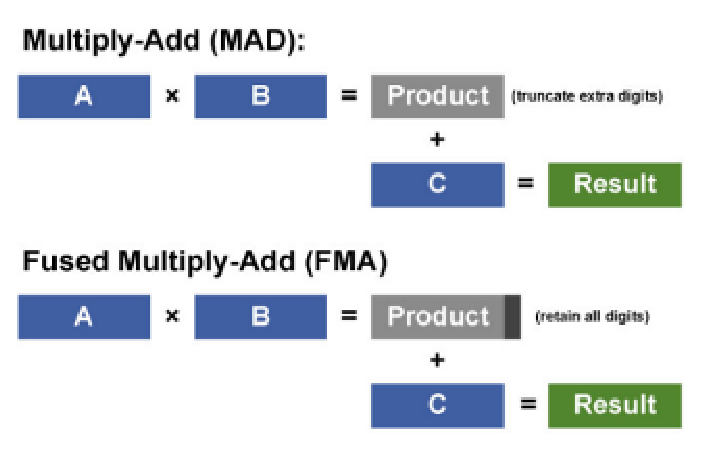
\includegraphics[height=4cm,
        angle=0]{./images/FMAD.eps}}
      \caption{Fused Muliply-Add (FMAD) in Fermi}
      \label{fig:FMAD}
    \end{figure}

\subsection{Streaming Multiprocessor (SM)}
\label{sec:stre-mult-sm}

{\bf SM configuration}: Each SM is composed of a number of SPs and some
supporting units. A streaming multiprocess (SM) is a complete computing unit
with components like instruction fetch and instruction dispatcher.

\begin{enumerate}
  \item Tesla-1 SM	 - Sect.\ref{sec:SM-Tesla-1}
  
  \item Tesla-2 SM - Sect.\ref{sec:SM-Tesla-2}
  
  \item 
\end{enumerate}

\subsection{-- Tesla-1 (G80/G92) SM}
\label{sec:SM-Tesla-1}

Tesla 1st gen: with 128 single-precision SPs (no double-precision core)
  
Each SM is composed of 8 SPs + 2 SFUs + 1 MT issue + 1 I-cache + 1 C-cache +
16KB shared-memory + 16KB L1 texture-cache + 8K 32-bit registers + 1 WARP scheduler
    
\begin{itemize}
  \item  $\rightarrow$ the chip has total 16 SMs.
  % \item SPs in this generation are limited to 24-bit precision for
  %   multiplications. 

  \item A SFU unit are indeed a cluster of several units that can
    handle unusual and exceptional operations in GPU,
    e.g. transcendental functions (sin(), cos(), reciprocal,
    square-root, exp()...), interpolation for parameter blending. For
    a list of supported special instructions, read
    Sect.~\ref{sec:special-instructions}. Each SFU executes one
    instruction per thread, per clock. So, a warp (32 threads)
    executes over 16 clocks.  Instructions which are natively executed
    by the SFU have \textcolor{red}{a 16 clock cycle latency}, while
    more complicated functions, e.g. square roots or exponentiation
    are synthesized by the compiler using a combination of
    instructions and take \textcolor{red}{32 clock cycles or longer}
    to execute. SFU hardware for interpolations include several 32-bit
    FP multiply units (FMUL), which can be issued separately for
    multiply instruction.

    SFU is physically implemented by 2 execution units: each one
    services 4 of the 8 execution pipelines in the SM; and multiply
    instructions issued to the SFU in the same
    \textcolor{red}{4 clock cycles} as in the FMAD unit.

  \end{itemize}

\subsection{-- Tesla-2 (GT200) SM}
\label{sec:SM-Tesla-2}

Tesla 2nd gen: with 240 single-precision SPs.

This is known as the second-generation SM, Fig.~\ref{fig:SM}.
Each SM is is composed of 8 SPs + 2 SFUs + 1 MT issue + 1 I-cache
+ 1 C-cache + 24KB shared-memory + 24KB L1 texture cache + 1
64-bit FMAD unit + 16K 32-bit registers + 1 WARP scheduler, as
shown in Fig.~\ref{fig:gt200_sm}, $\rightarrow$ total 30 SMs.
    
\begin{itemize}
  \item A new unit - the double precision fused-multiply-add (FMAD)
    unit (FP64-unit) has been added which supports standard IEEE 754-1985
    behavior, with full speed de-normal handling and classic 64 bit integer
    arithmetic. 
    
In GT200, a brand new 64-bit FMAD shared by the entire SM for integer
and floating point computation that relies on the new support 64-bit
register files. This is also a double-precision FMA unit (support
standard IEEE 754-1985), with full speed de-normal handling and
classic 64-bit integer arithmetic. 

In total, GT200 has 30 FP64 units.
\end{itemize}

\begin{figure}[hbt]
  \centerline{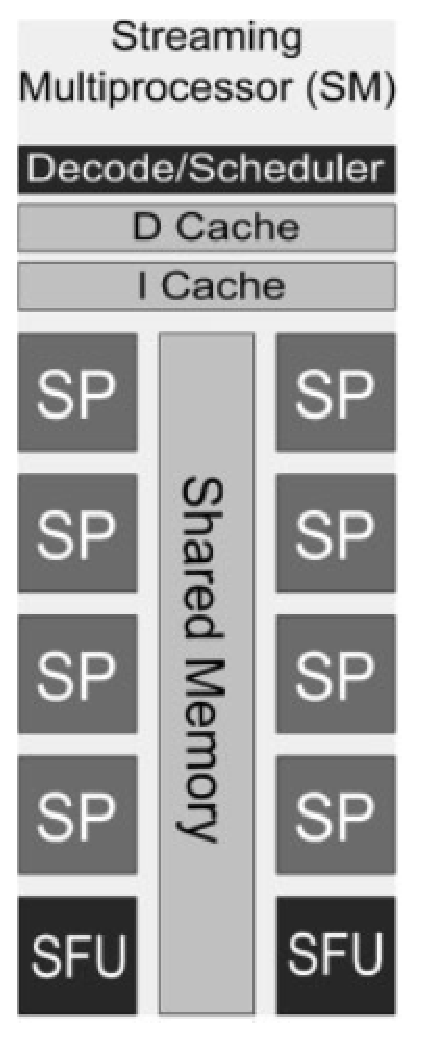
\includegraphics[height=5cm,
    angle=0]{./images/SM_GT200.eps}}
 \caption{SM of GT200}
\label{fig:SM}
\end{figure}


\begin{framed}
  FMAD performs a fused multiply-add with a single rounding on the
  result, i.e. enabling more accurate result (especially on iterative
  algorithms).  Even though using FMAD improve the accuracy, it
  decreases the performance, as the number of FMAD units is 1/4 of
  double-precision units in Fermi.  In GT200, every 8 SPs has one
  separate double-precision core, then using double-precision
  computation may decrease the performance by a factor of 8 (to be
  explained in detail in Sect.~\ref{sec:cuda-apis}.
\end{framed}

\subsection{-- Fermi (GF100) SM}
\label{sec:SM-Fermi}

Fermi: use GF100 chip (planned: 512) with 448 single-precision SPs due to design
limitations. \textcolor{red}{This is known as the third-generation SM which has
a lot of innovations}. 
\begin{enumerate}
  \item First is the addition of a Texture Unit which previously
is not part of an SM.
  
  \item  In earlier Tesla GPU, a SM doesn't have cache, which is an essential
  component
in modern CPU. In Fermi GPU, a SM have both shared memory and L1/L2 cache.

   \item implemented a unified GPU address space spanning the three main GPU
   memory spaces (thread private local memory, thread block shared memory, and
   global memory). 
   
This unified address space, however, only applied to GPU memory addressing, and
mainly resulted in simpler compilation by enabling a single load/store
instruction and pointer address to access any of the GPU memory spaces (global,
local, or shared memory), rather than different instructions and pointers for
each. This also enabled full C and C++ pointer support, which was a significant
advancement at the time.
\end{enumerate}

That's why Fermi GPU is considered as the most complete GPU design in that its
SM is most similar to a CPU. 

 \begin{framed}
    
    Rather than at TPC level, 4 TEX units now resides within each SM
    and is clocked at 1/2 the speed of CUDA cores. However, this speed is 
    still higher
    than those in GT200.
    % Thus, we no longer need a separate 64-bit arithmetic unit.
  \end{framed}  

Each SM is composed of 
\begin{itemize}
  \item 32 redesigned SPs - Sect.\ref{sec:SP-Fermi}

Every SM now has 32, rather than 8 SPs. 
        
  \item 4 SFUs 

 With 4 SFU units,
    \textcolor{red}{a warp execute over 8 clock cycles}. The SFU
    pipeline is decoupled from the dispatch unit, allowing the
    dispatch unit to issue to other execution units while the SFU is
    occupied.

  \item 1 MT issue 

  \item 1 I-cache 
  
  \item  1 uniform-cache (replacement for C-cache) 
  
  \item 64KB shared-memory/L1 cache +
\textcolor{red}{12KB Texture-cache} + 32K 32-bit registers 

New L1 cache/shared-memory configuration allows compiler to
    manage between 16/48 (suitable for graphics application) and 48/16
    (suitable for compute apps), Fig.~\ref{fig:L1_L2}.
    \textcolor{red}{NOTE: The setting is discussed in Sect.~\ref{sec:shared-memory-cache}}.

L1 cache is to store data only for that SM, but share-memory cache is shared
between all SMs. So, depending on your application (whether you want to share
much data between SM or not), you can adjust the amount of L1/share-memory to
match the application's demand. The default is (see next).

  \item 2 WARP schedulers + 2 I-Dispatch Units 
 
  Third generation SMs, with 2 warp-schedulers, can process 2 warps
    at the same time. With 32 SPs per SM, each warp uses 16 SPs, given
    that 32-bit operations are used. If threads use 64-bit operations,
    only a single instruction can be issued as two 32-bit units will
    handle a single 64-bit operation.  

 2 (dual) WARP schedulers + 2 Instruction Dispatch Units allow
    2 warps to be executed concurrently. So, for each warp, an
    instruction is issued to a group of 16 cores, 16 LD/ST units,
    or the 4 SFUs units.
\begin{figure}[hbt]
  \centerline{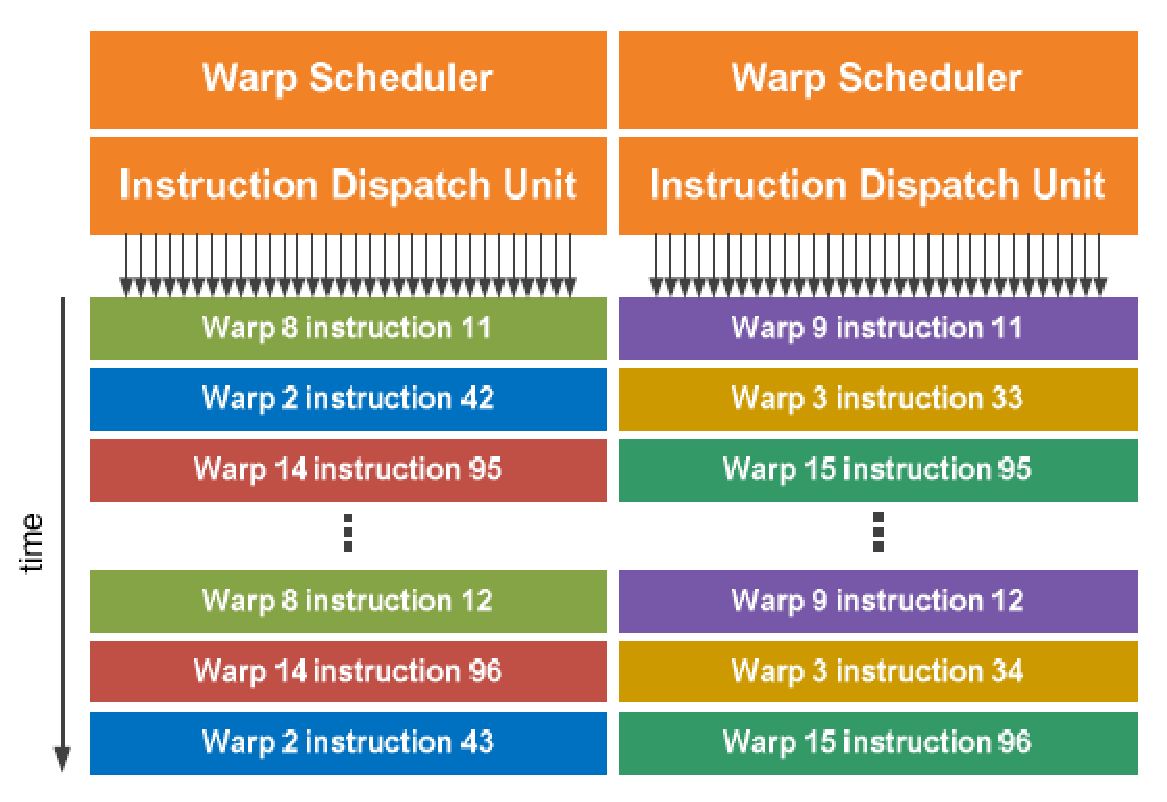
\includegraphics[height=5cm,
    angle=0]{./images/dual_warp_scheduler.eps}}
\caption{Fermi's dual-warp scheduler}
\label{fig:dual_warp_scheduler}
\end{figure}
As shown in Fig.~\ref{fig:dual_warp_scheduler}, the dual-warp
scheduler select 2 warps (to be active), issue one instruction to each
warp. As inter-warp threads are independent, using dual-warp mechanism
can achieves near-peak performance. However, double-precision and
special-purpose unit (SPU) operations (like exp(), sin()...) do not
support dual-dispatch with any other operations.
\textcolor{blue}{Others instructions can be dual-issued (e.g. two
  integer instructions, two floating instructions, or a mix of
  integer, floating point, load, store, and SFU instructions).}
 
  \item 4 TEX units + 1 PolyMorph Engine + 16 load/store (LD/ST) units.

TEX units run at half of the shader clock speed (NOTE: 1/2 shader clock
  speed = core clock). 
  
NOTE: TEX units in GT200 run at the same speed at graphics
  core clock, Fig.~\ref{fig:texture_performance}.

    \begin{figure}[hbt]
      \centerline{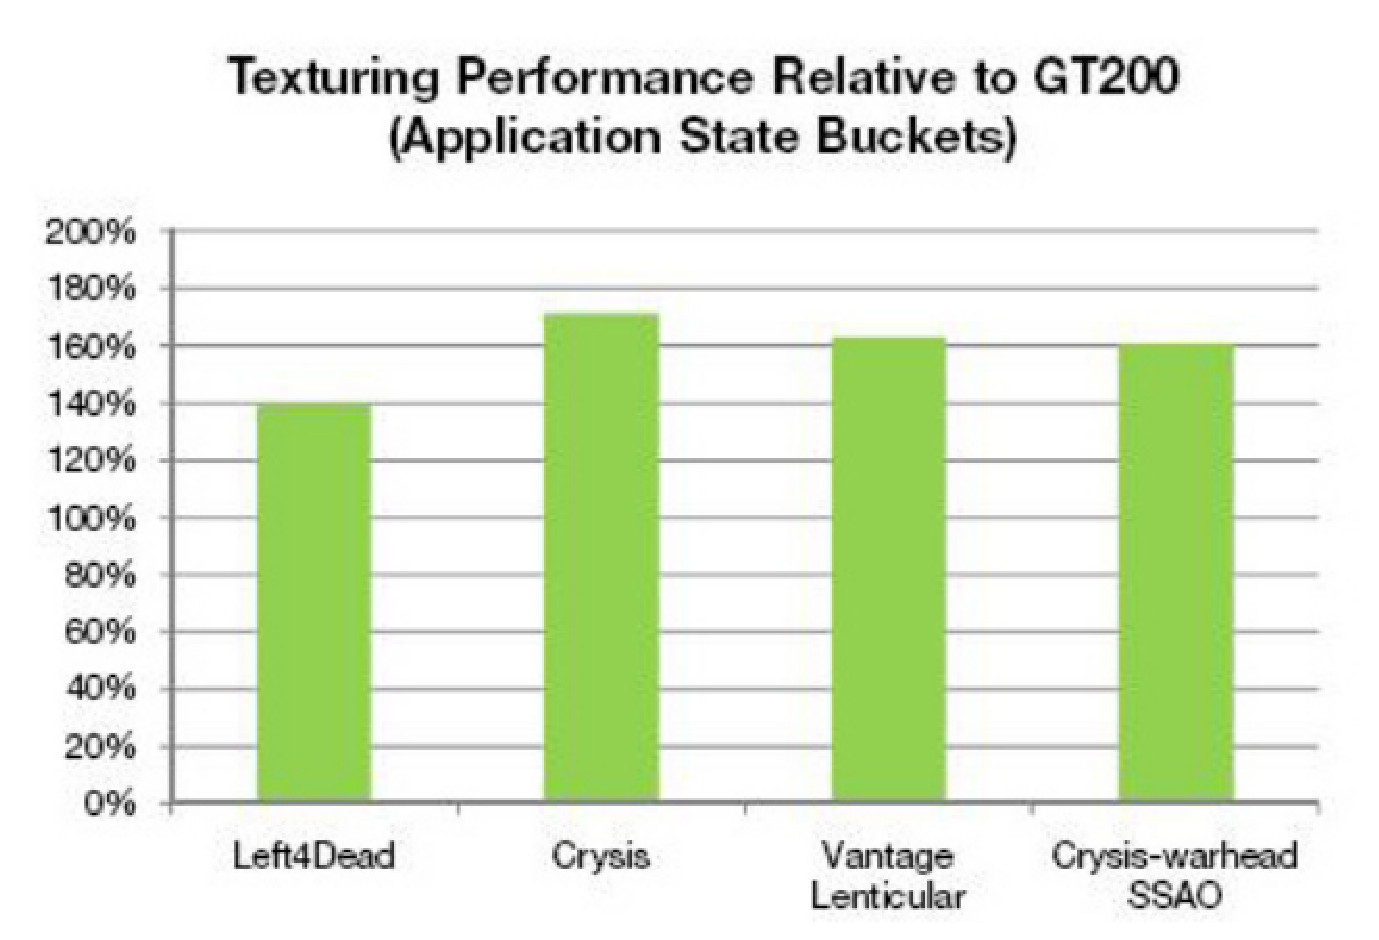
\includegraphics[height=5cm,
        angle=0]{./images/texture_perf.eps}}
      \caption{Texture performance in some applications (GF100 vs. GT200)}
      \label{fig:texture_performance}
    \end{figure}

\end{itemize}


\begin{figure}[hbt]
  \centerline{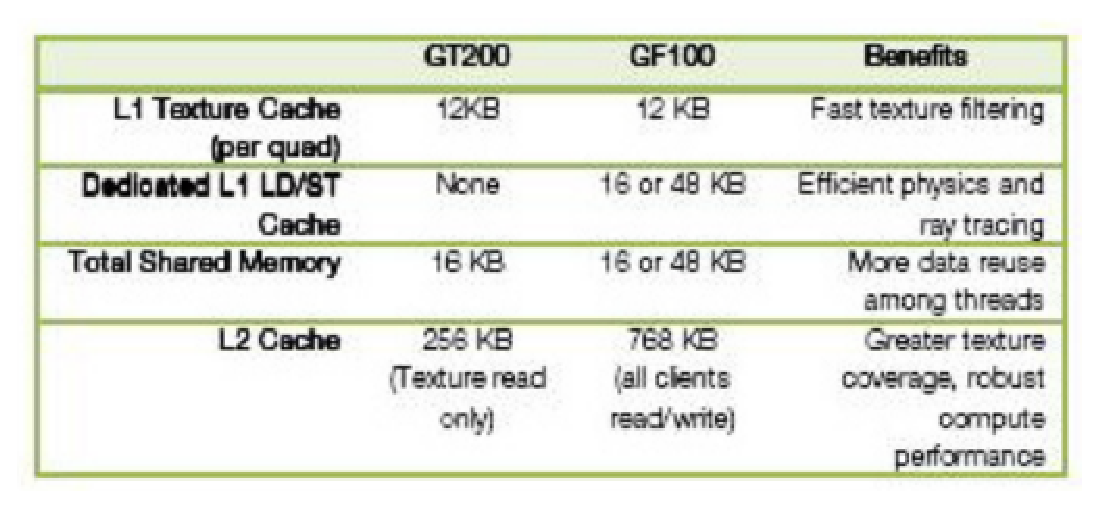
\includegraphics[height=4cm,
    angle=0]{./images/L1_L2_cache.eps}}
  \caption{L1 and L2 cache (NOTE: L2 cache is at chip level which
    means it's shared by all SMs and is particularly useful when all
    SMs need to access the same data). In GT200, L2 cache is indeed L2
    texture cache as it is dedicated to texture read only (CUDA
    Fortran 2010 doesn't support reading texture cache)}
\label{fig:L1_L2}
\end{figure}

\subsection{-- Kepler (GK10) SMX}
\label{sec:SM-Kepler}
\label{sec:Kepler_SMX}
  
Kepler (CC 3.0): use GK10 chip 

Most of the key hardware units for graphics processing reside in the SM.
A major change in Kepler-based GPU is the concept of {\bf SMX} (Shader
Multiprocessor, Shader Multiprocessing Engine), rather than using SM (streaming
multiprocessor), Fig.\ref{fig:Kepler_SMX}. Each SMX has


Each SM now has 
\begin{itemize}
   \item 192 SP (CUDA core for arithmetic operations), 
   
   \item 32 special function units (SFU) for handling single-precision floating-point
   transcendental functions, 
   
   
   \item 4 WARP schedulers.
 
 Each WARP scheduler can issue 2 independent (single-precision)
   instructions of a time (or one double-precision instruction).
   \textcolor{red}{SM is now 6x more SP and SFU}, but 2x more WARP scheduler.
   Maybe they see that the overal latency for each instruction is large so it's
   better to launch more instructions at once to mask the latency.
   
   With 4 WARP scheduler, Kepler K10 can executes 8 (single-precision)
   instructions from 4 different warps at a time. 
   
   \item L1 cache 
 \end{itemize}
   
\begin{figure}[hbt]
\centerline{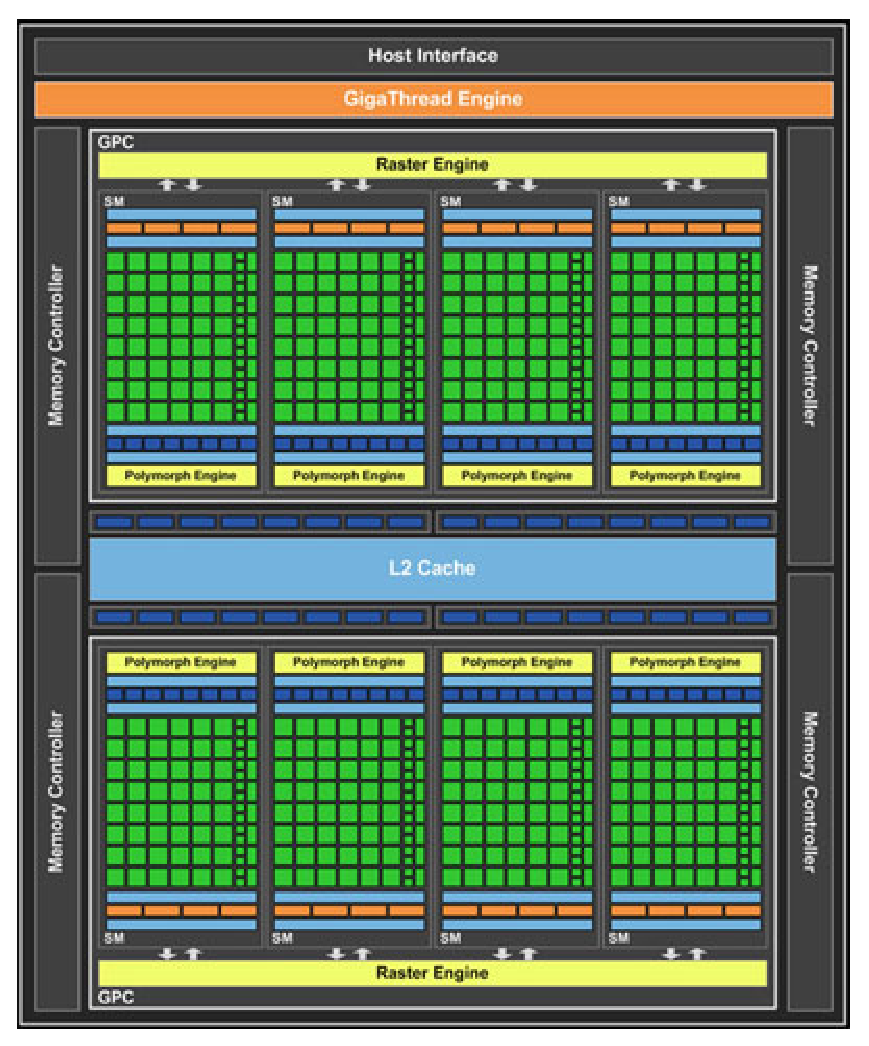
\includegraphics[height=7cm,angle=0]{./images/GF104.eps}
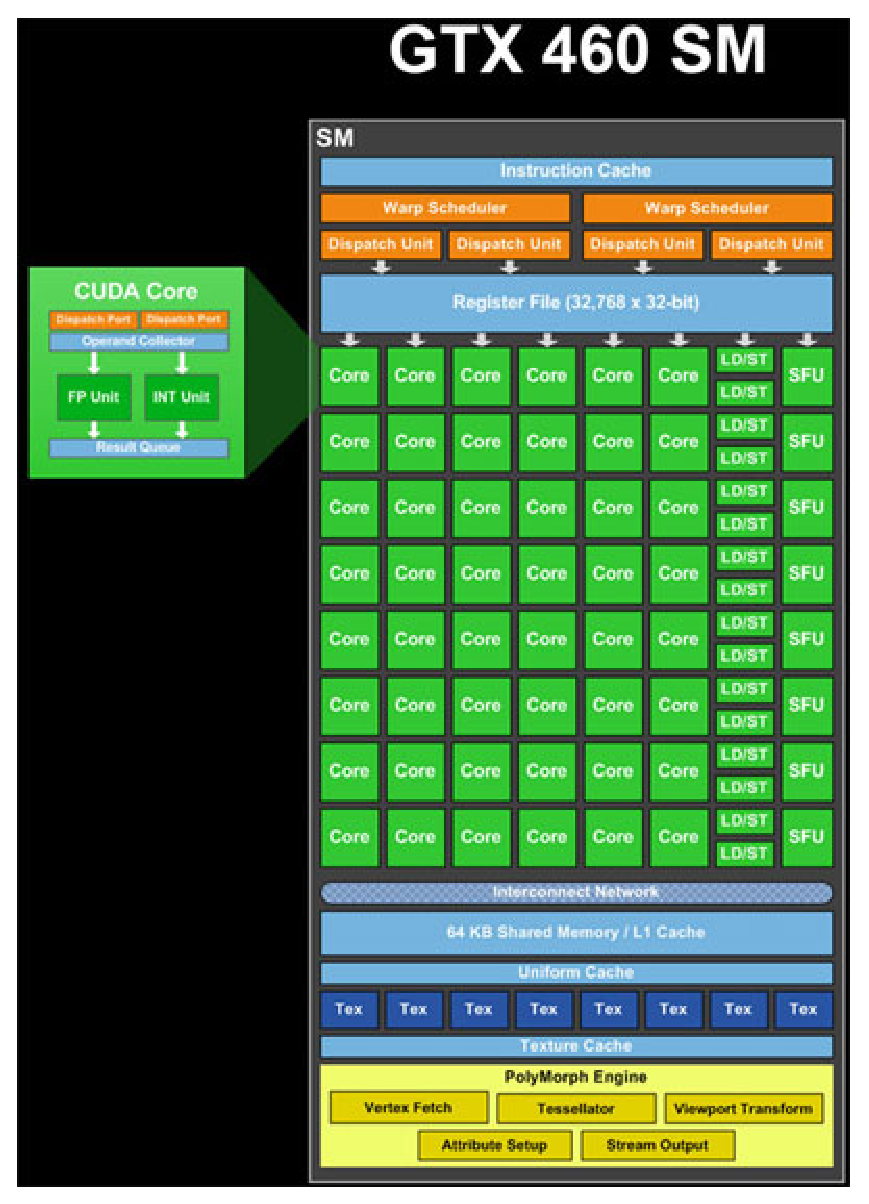
\includegraphics[height=5cm,angle=0]{./images/GF104_SM.eps}}
\caption{GTX 460 SM based on GF104. A GTC in GF104 has 48 SPs}
\label{fig:GF104}
\end{figure}

\begin{framed}
  SM can work with shaders of any types (vertex, pixel, geometric),
  and process them using its scalar processors.  Each SM is loosely
  considered as a modern microprocessors with 8-wide SIMDs. The
  front-end of each SM is (1) an instruction fetch, (2) decode and
  issue logic, (3) execution units. Thus, in the context of OpenCL, SM
  is called {\bf compute unit}.
\end{framed}

\subsection{-- Maxwell (GM200) SM}
\label{sec:SM-Maxwell}


\subsection{-- Pascal SM}
\label{sec:SM-Pascal}

Each SM has 64 CUDA Cores and four texture units (TEX units).

\begin{itemize}
  \item   64 single-precision (FP32) CUDA Cores

 In contrast, the Maxwell and Kepler SMs had 128 and 192 FP32 CUDA Cores,
 respectively.
 
 While a GP100 SM has half the total number of CUDA Cores of a Maxwell SM, it
 maintains the same register file size and supports similar occupancy of warps
 and thread blocks.

  
  \item 
\end{itemize}

\subsection{Texture Processing Cluster (TPC)}
\label{sec:TPC-TextureProcessingCluster}


{\bf Texture Processing Cluster (TPC) configurations}: All texture functions are
processed inside a TPC. A single GPU chip is a configuration of TPC.
\begin{enumerate}
  \item Tesla-1 TPC
  \item Tesla-2 TPC
\end{enumerate}

Since Kepler, TPC is replaced by GPC (Sect.\ref{sec:GPC}).


\subsection{-- Tesla-1 TPC}

Tesla 1st gen:     have 8 TPCs.

Each TPC is composed of 
\begin{itemize}
  \item 2 SMs 
  
  \item 1 TEX engine (texture unit) 
  
  \item 1 geometry controller (GC) 

  \item 1 SM controller (SMC). 
\end{itemize}


\subsection{-- Tesla-2 (GT200) TPC}

Tesla 2nd gen: have 10 TPCs.

Each TPC is composed of
  \begin{itemize}
  \item 3 SMs 

  \item 1 TEX engine (which contains 8
    texture filtering units)
    
  \item 1 geometry controller (GC) 
  
  \item 1 SM controller (SMC). 
\end{itemize}

\subsection{-- Pascal TPC}
\label{sec:TPC-Pascal}


Each TPC of GP100 has two SMs.



\subsection{TPC to GPC}
\label{sec:tpc-gpc}
\label{sec:GPC}

GT200 has 3 levels (excluding SP): GPU, TPC and the SM. This is a complex
structure and Nvidia decided to rethink it completely in Kepler GPU. 

With the Texture Unit moved into the SM in Kepler GPU, there's no need to use
TPC. Instead, a new concept is developed called GPC ({\bf Graphics Processing
Cluster}) which is a considered as a self-contained GPU.

Most GPU's graphics functions are performed inside the GPC. In GT200, the whole
chip has only a single {\it Raster Engine}. Now, in Fermi, each GPC is equipped
with a Raster Engine, which allows it to function as a self-contained GPU.  This
is the reason the name was given.

\subsection{-- Fermi (GF100) GPC}
    
In Fermi, each GPC has a 
\begin{enumerate}
  \item one Raster Engine: triangle setup, rasterization, z-cull
  \item four SMs
  
The size of SM in Fermi (32 SPs (GF100) or 48 SPs (GF104)) is different from
previous version of GPUs (8 SPs); 

NOTE: some components (e.g. TEX units...) are moved to the SM level (read
Sect.~\ref{sec:stre-mult-sm}), Fig.\ref{fig:Fermi_GPC}.

\end{enumerate}


Ideally, a Fermi card has 4 full GPCs. However, due to the limitation of 40nm
architecture, in the last GPC of GF100 chip, two SMs are disabled. From GF110
chip, all four GPCs has the full 4 SMs.

With 4 GPCs, a Fermi chip have 16 SMs. However, two are disabled, and total 14
SMs are enabled. \footnote{ Tesla 3rd gen was expected to have 512 cores (with
16 SMs); yet due to limitation of 40nm architecture, current Fermi has only 14
SMs enabled}.

\begin{figure}[hbt]
  \centerline{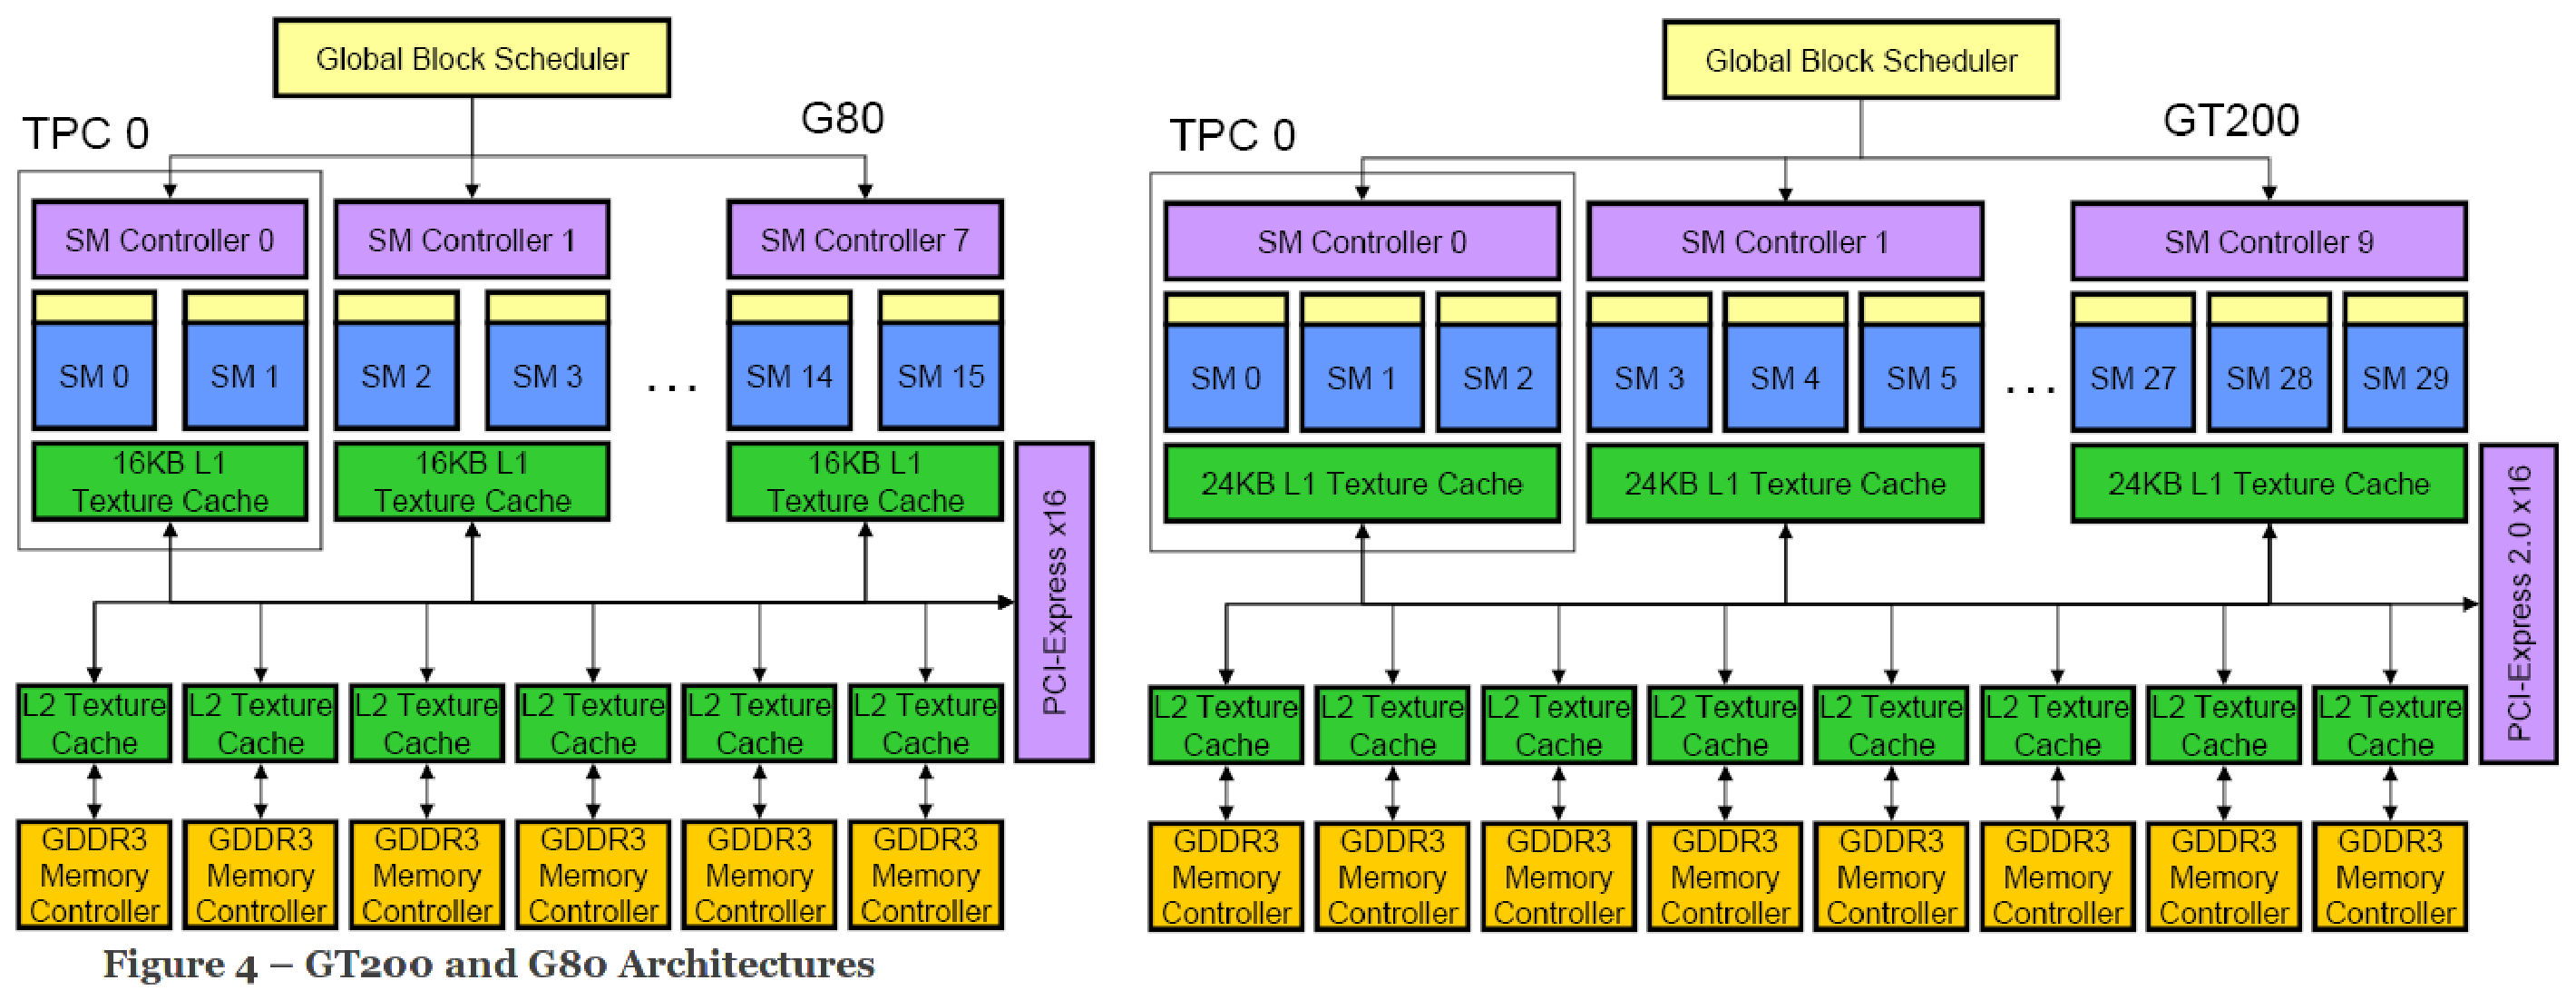
\includegraphics[height=5cm,
    angle=0]{./images/g80_gt200.eps}}
  \caption{G80 and GT200 architectures}
  \label{fig:g80_gt200}
\end{figure}

\begin{framed}

GF104:  While GF100 has 4 GPCs (each with 4 SMs, each SM with 32 SPs); GF104 has
2 GPCs, each also with 4 SMs; yet now \textcolor{red}{each SM with
  48 SPs}, Fig.\ref{fig:GF104}. GF104 has one SM disabled; so it has 7*48= 336
  SPs totally. To balance the increase in SPs/SM, GF104 has double the number of
  instruction dispatch (to 4), and the number of texture units (to 8) per SP.
  So, it supports higher concentration of texture performance than shader
  performance compared to GF100.
\end{framed}

\begin{framed}
  The term ``cluster'' is also referred to as GPC. An SM is called a
  ``subcluster''. AMD's Cypress GPU is 20-cluster part, and Nvidia's
  GT200 is 10-cluster part.

  Nvidia calls the unit group of threads running simultaneously is
  {\bf warp}, yet AMD calls it {\bf wavefront}. For Nvidia, a warp is
  32 threads. For AMD, a wavefront is 64 threads. 
\end{framed}

\begin{figure}[hbt]
  \centerline{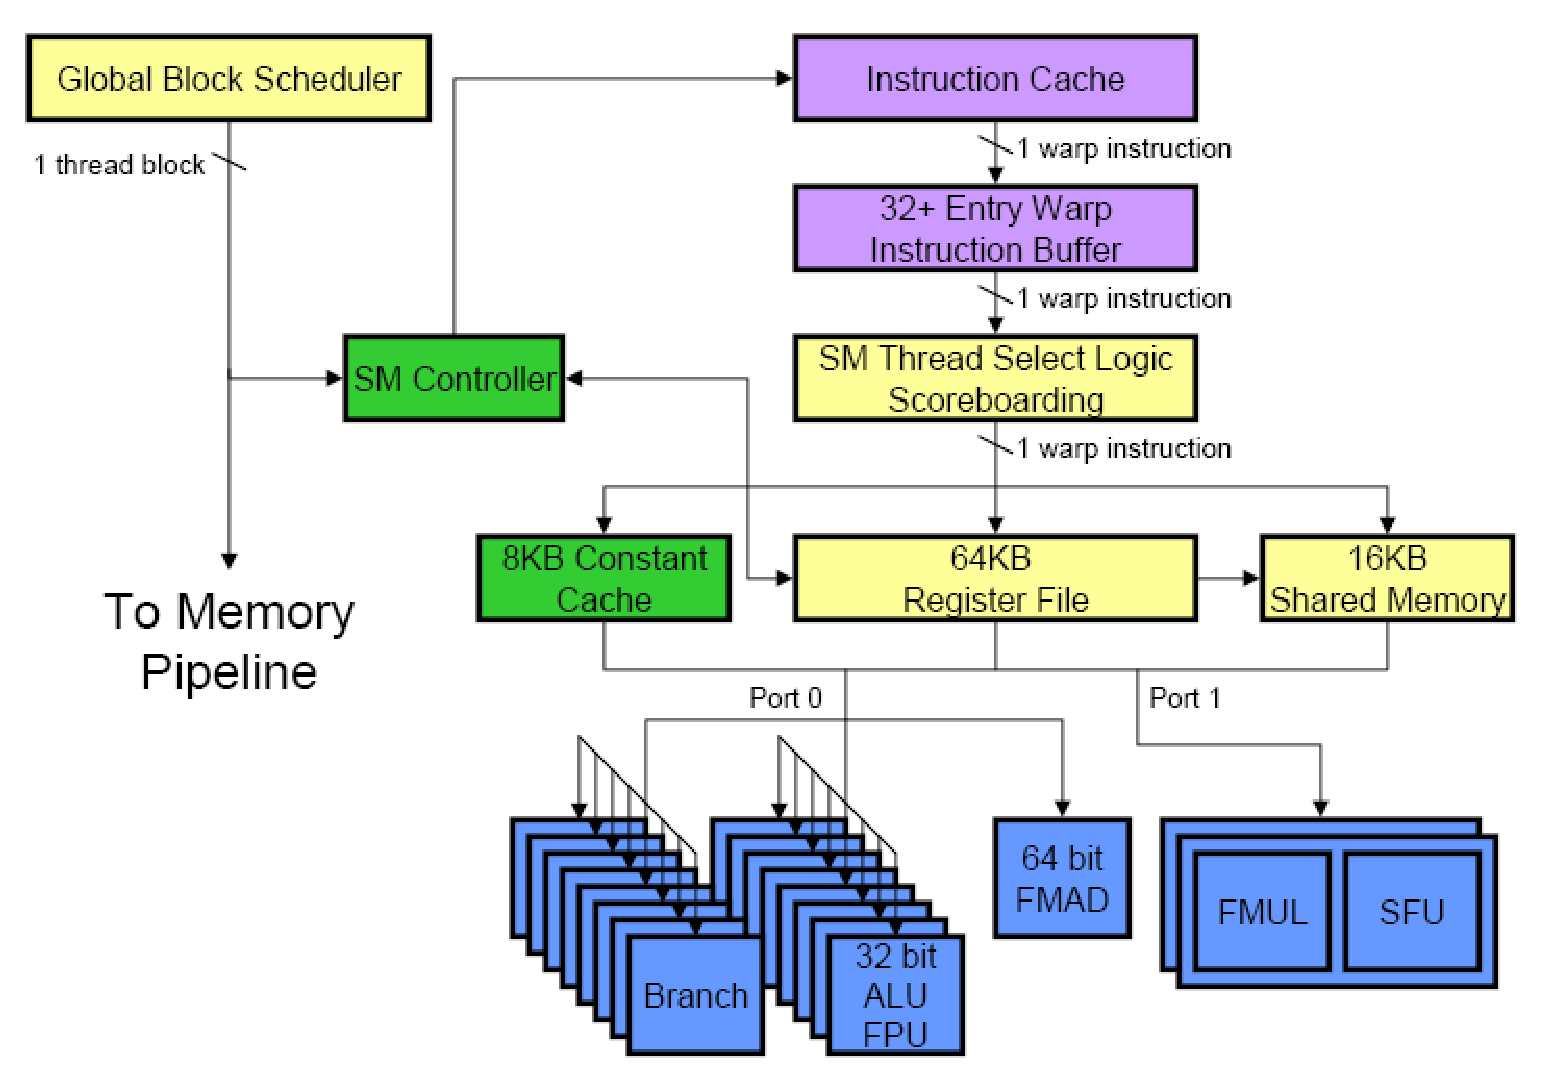
\includegraphics[height=7cm,
    angle=0]{./images/gt200_sm.eps}}
  \caption{Architecture of a GT200 streaming multiprocessor\footnote{\url{http://www.realworldtech.com/page.cfm?ArticleID=RWT090808195242&p=9}}}
  \label{fig:gt200_sm}
\end{figure}


\begin{figure}[hbt]
  \centerline{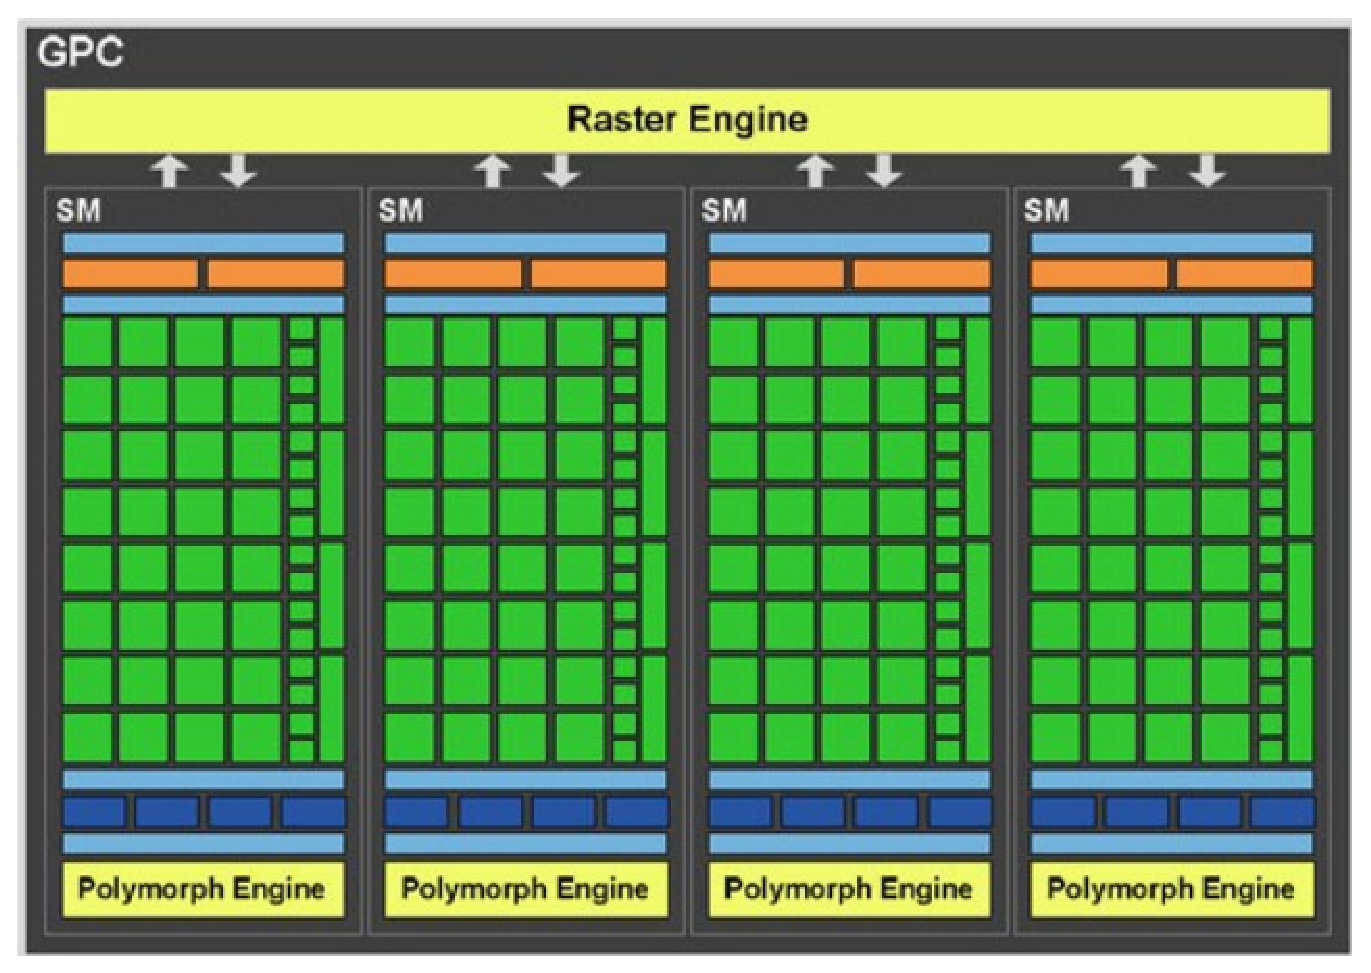
\includegraphics[height=5cm,
    angle=0]{./images/Fermi_GPC.eps}}
  \caption{A single GPC in GF100 architecture}
  \label{fig:Fermi_GPC}
\end{figure}


In Fermi, the number of double-precision CUDA cores is 7x times than
those in GT200. However, the speed-up that we can reach in many
applications is lower than that, e.g. about 4x in matrix
multiplication, Fig.~\ref{fig:matrix_mul}. The reason is that other
resources (registers, shared memory...) don't increase of that same
factor. 

\begin{figure}[hbt]
  \centerline{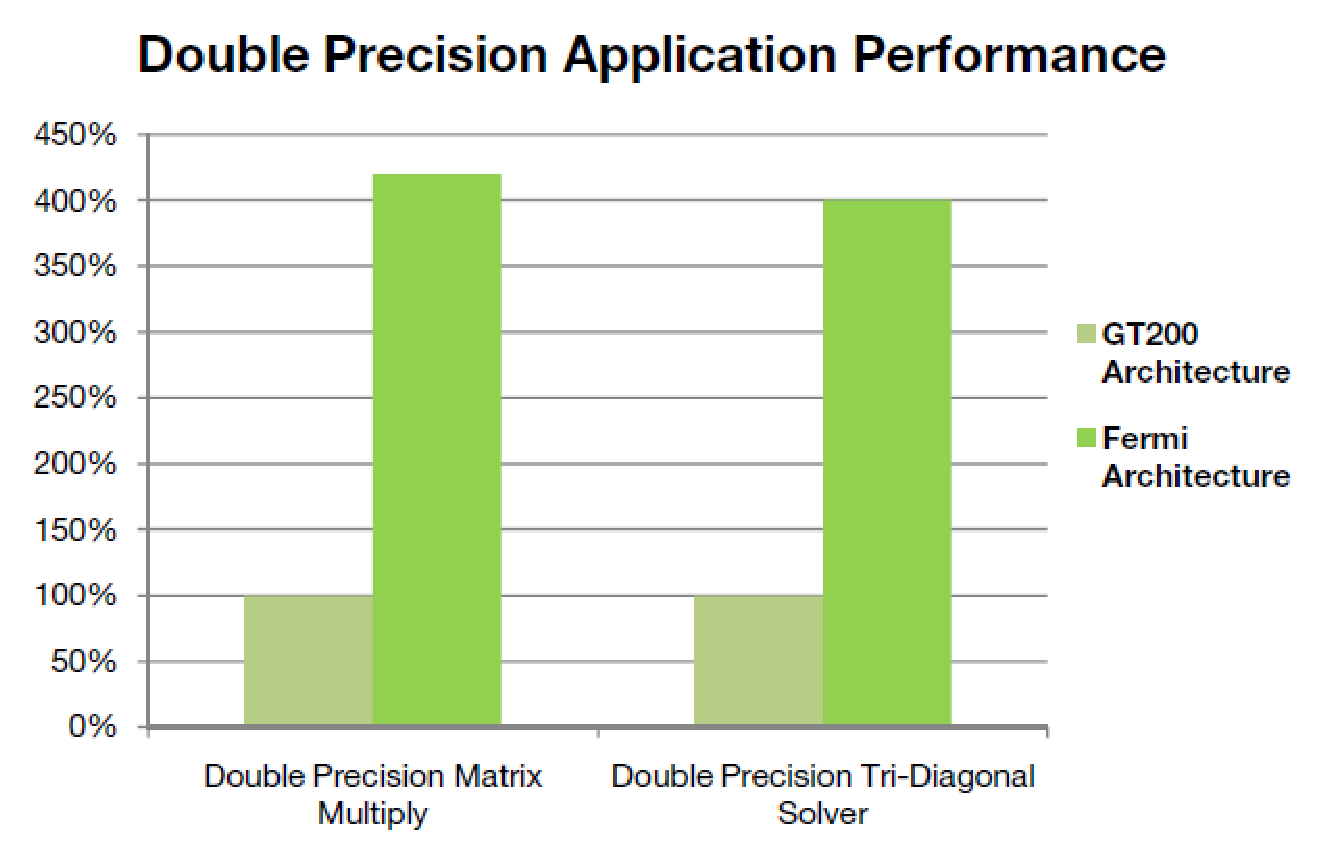
\includegraphics[height=5cm,
    angle=0]{./images/matrix_mul_fermi.eps}}
  \caption{Early performance evaluations show Fermi performing up to
    4.2x faster than GT200 in double precision applications.}
\label{fig:matrix_mul}
\end{figure}


\subsection{-- Maxwell (GM200) GPC}
\label{sec:GPC-Maxwell}

Tesla M40 (GM200) has 24 SMs or 24 TPCs

\subsection{-- Pascal (P100) GPC}
\label{sec:GPC-Pascal}

GP100 is composed of an array of Graphics Processing Clusters (GPCs), Texture
Processing Clusters (TPCs), Streaming Multiprocessors (SMs), and memory
controllers.


A full GP100 consists of six GPCs (equivalently to 60 SMs). However,
Tesla P100 accelerator uses 56 SM units or, equivalently, 28 TPCs.

With 60 SMs, GP100 has a total of 3840 single precision CUDA Cores and 240
texture units.

\begin{itemize}

  \item Each GPC inside GP100 has ten Pascal SMs (Sect.\ref{sec:SM-Pascal})
  
  \item 30 TPCs (each including two SMs).
  
  
  \item Eight 512-bit memory controllers (4096 bits total). 

  NOTE: Each memory controller is attached to 512 KB of L2 cache, 

  \item Each HBM2 DRAM stack is controlled by a pair of memory controllers. The
  full GPU includes a total of 4096 KB of L2 cache.

\end{itemize}



\section{Warp scheduler}
\label{sec:warp-scheduler}

Threads are organized into groups called warp (i.e. Nvidia uses 32 threads per
warp). All threads in the same warp execute the same instruction. When branching
occur, they are executed one by one. During the execution of one branch, only
threads satisfying the condition execute, other threads in the warp need to
wait. 

The warps are selected to use the processors by the {\bf warp scheduler}. In
Fermi, with 2 warp schedulers, two warps can be activated at once. The
instruction of threads in one warp is sent to the CUDA cores in one SM by the
instruction dispatch units. With 2 warp scheduler, it also need 2 instruction
dispatch units, each one issues one independent instruction from one warp.

Processors are selected in groups to execute the instruction. In Fermi, a group
of 16 CUDA cores are selected at once to run the instruction. The data are
loaded using the 16 LD/ST units [NOTE: Earlier Tesla selecte CUDA cores in
group of 8]. 

In most cases, two instructions from two warps can be issued at once (e.g. two
integer instructions, two floating instructions or a mix of integer, floating
point. However, double-precision instructions do not support dual dispatch with
any other instructions. So, if one warp execute a double-precision instruction,
the other warp need to wait until the double-precision is dispatched. [NOTE:
This restriction is removed in Kepler].

References:
\begin{itemize} 
  \item in Fermi: \ref{sec:warp-scheduler-fermi}
  \item 
\end{itemize}

\section{Texture (TEX) unit}
\label{sec:texture-unit}

In Tesla 1 and 2, texture units and L1 texture cache are at TPC level,
where 2 or 3 SMs shares one texture unit and one L1 texture cache. The
purpose of TEX unit is to rotate or resize bitmap to be placed on an
arbitrary 3D object as a texture. Each TEX unit computes a texture address and
fetches 4 texture samples per clock. The results can be filtered or
unfiltered. Different filter modes can be used: bilinear, trilinear and
anisotropic.



\subsection{Texture (TEX) unit}
\label{sec:texture-unit-Fermi}

TEX unit is described in Sect.\ref{sec:texture-unit}. In GF100, TEX unit and L1
texture cache have been brought to SM level. Each SM has 4 texture units.

Each unit could compute 1 texture address and fetch 4 32bit/INT8 texture samples
\textcolor{red}{per 1 clock}, 2 64bit/FP16 texture samples \textcolor{red}{per
clock}, or 1 128bit/FP32 texture sample \textcolor{red}{per clock}. 

Texture units and L1 Texture caches at SM level can run at higher clock speed
[NOTE: texture units on previous architecture run at the core clock of GPU].

With unified L2 cache, the maximum cache size for texture is 3x higher than
GT200, improving hit rates in texture heavy shaders. 

GK100 texture unit supports for
\begin{enumerate}
  \item  DirectX 11's BC6H and BC7 texture compression formats.
  \item jittered sampling, i.e. DirectX 11's four-offset Gather4 feature in
  hardware (allowing 4 texels to be fetched from a 64x64 pixel grid with a
  single texture instruction).
\end{enumerate} 

GF104 texture units improved this to 4 samples/clock for both 32bit
and 64bit, and it's these texture units that have been brought over
for GF110. GF110 can now do 64bit/FP16 filtering at full speed versus
half-speed on GF100, and this is the first of the two major steps
Nvidia took to increase GF110's performance over GF100's performance
on a clock-for-clock
basis\footnote{\url{http://www.anandtech.com/show/4008/Nvidias-geforce-gtx-580/2}},
Fig.~\ref{fig:texture_unit}.

\begin{figure}[hbt]
  \centerline{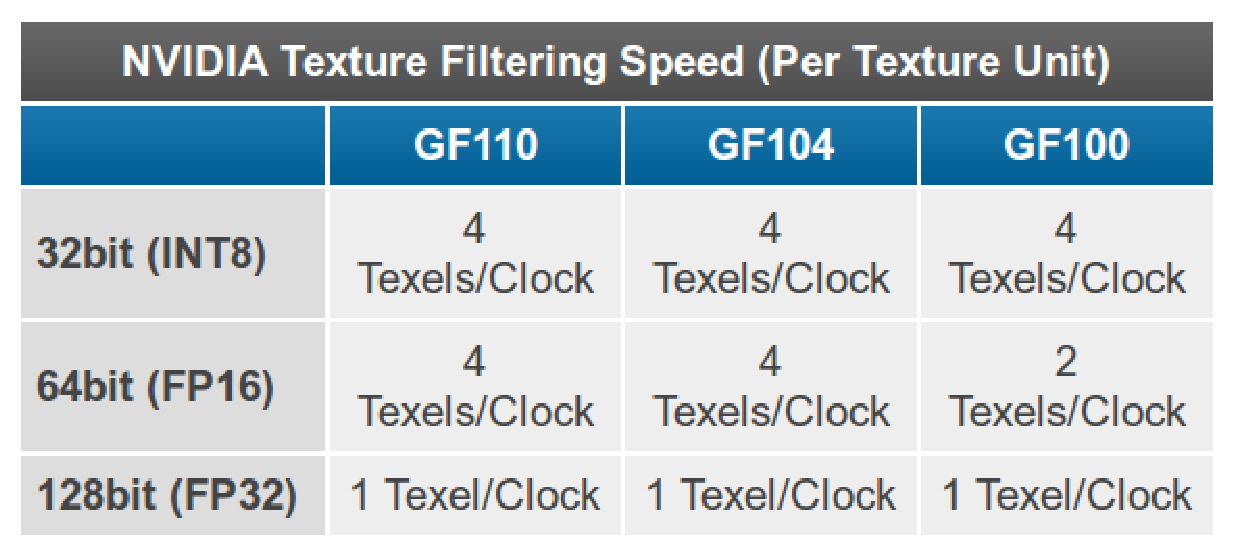
\includegraphics[height=5cm,
    angle=0]{./images/texture_unit.eps}}
  \caption{Texture units}
  \label{fig:texture_unit}
\end{figure}

\section{PolyMorph Engine}
\label{sec:PolyMorph-Engine}


\subsection{PolyMorph Engine (geometry unit)}
\label{sec:polymorph-unit-+}

PolyMorph Engine in Kepler is version 2.0. 

GT200 has only a single PolyMorph engine residing at the front-end of
the graphics pipeline. Thus, the traditional pipeline has tessellation
unit in the front of the pipeline with the (edge) setup and
rasterization units (as in AMD/ATI RV870). This can be a bottle neck
where tessellation is utilized heavily. 

Nvidia revolutionized this to enable high triangle rates under the most
demanding scenarios by incorporating a hardware {\it tessellator unit} in
PolyMorph Engine and provide each SM a PolyMorph engine.

As described in Sect.\ref{sec:Fermi_graphics-enhancement}, a newly-designed
Polymorph Engine is a new execution unit developed in Nvidia Fermi GPU card.

{\bf Each SM in Fermi has one PolyMorph Engine}. PolyMorph Engine is the execution
unit that handle geometry in 5 stages: Vertex Fetch, Tessellation, Viewport
Transform, Attribute Setup, and Stream Output. This design support DirectX11,
where Tessellation is brought from CPU to GPU
design\footnote{\url{http://www.anandtech.com/show/2918/2}}.

Each PolyMorph Engine contains a Tessellation Unit, an Vertex Fetch (Attribute
Setup) Unit, and other Geometry Processing Units. Along with this is the use of
4 Raster Engines, which allowing 4 triangles to be setup per clock. Together,
they enable breakthrough triangle fetch, tessellation, and rasterization
performance.

\textcolor{red}{The results from one stage are sent to the SM to
  process; and then sent back to the next stage. At the last stage,
  the results are sent to the Raster Engine}.
\textcolor{blue}{The Tessellator is one of the biggest change that
  DX11 brought to GPU design}
to be well used in DX11 and future
games)\footnote{\url{http://www.anandtech.com/show/2977/Nvidia-s-geforce-gtx-480-and-gtx-470-6-months-late-was-it-worth-the-wait-/3}},
Fig.~\ref{fig:polymorph}.


\begin{framed}
Tessellation is a vertex operation (tesselation adds extra geometry detail
on-the-fly for less angular objects and characters).
\end{framed}

The {\bf geometry pipeline} (geometry unit) has been significantly
revamped with improved performance in geometry shading, stream out,
and culling. Fillrate has also been improved which enables multiple
displays to be driven simultaneously by GF100 SLI, much like AMD's
Eyefinity; but now additionally in 3D and at 120 Hz.

\begin{framed}
  In Fermi, each SM has a PolyMorph engine $\rightarrow$ GF100 has 16
  PolyMorph Engines (indeed 2 of them are disable). Even though a
  single PolyMorph engine is still an in-order design, the
  availability of 16 different PolyMorph engines allows the
  Out-of-Order (OoO) execution, as GF100 need to keep track of what
  each engine is doing to maintain the integrity of the results. To do
  this, GF100 has a separate communication channel between the
  PolyMorph engines.
\end{framed}

\begin{figure}[hbt]
  \centerline{\includegraphics[height=2cm,
    angle=0]{./images/polymorph.eps}}
\caption{PolyMorph}
\label{fig:polymorph}
\end{figure}

A PolyMorph Engine handles vertex fetch, tessellation, viewport transform, 
attribute setup, and stream output
\begin{enumerate}
\item Vertex Fetch: fetching vertices from a
  {\it global vertex buffer}; then, these vertices are sent to the SM
  for vertex shading and hull shading. In these two stages the
  vertices are transformed from object space to world space, and
  calculate tessellation factors.

\item Tessellator: receive the tessellation factors and then dices the
  patch and outputs a mesh of vertices. The new vertices are sent to
  the SM where the Domain Shader and Geometry Shader are executed.

  The Domain Shader calculates the position of each vertex based upon
  input from the Hull Shader and the Tessellator. At this stage a
  displacement map is usually applied to add detailed features to the
  patch. The Geometry Shader conducts post processing adding and
  removing vertices and primitives where needed. The final results are
  sent to the Tessellator for the final pass.

\item ViewPort Transform: receive the result from SM, it performs viewport
  transformation and perspective correction. 

\item Attribute setup follows, transforming post-viewport vertex
  attributes into plane equations for efficient Shader evaluation.

\item Finally, vertices are optionally
  "streamed out" to memory making them available for additional
  processing\footnote{\url{http://www.motherboards.org/reviews/hardware/2038_4.html}}. 
\end{enumerate}

\begin{framed}
  
  The newly generated primitive shapes are converted to pixels using
  Raster Engines. GT200 has a single Raster Engine. In Fermi, every 4
  SMs has a Raster Engine. So, a group of 4 SMs in Fermi now can
  function as an individual GPU chip. Thus it is given the name
  Graphics Processing Cluster (GPC).  ATI RV870 has two raster
  engines.
\end{framed}


The total PolyMorph Engine in GTX 680 (Kepler) is 8, which is half of that in
GTX 580 (Fermi). However, the performance is roughly double per-clock of the
Fermi version. With 30\% higher in clock speed, it means the overal performance
of PolyMorph Engine in Kepler GTX 680 is higher than that in Fermi GTX 580, i.e.
a polygon is spurred in about 2 cycles in GK104 instead of 4 in GF100
\footnote{\url{http://www.tomshardware.com/reviews/geforce-gtx-680-review-benchmark,3161-2.html}}.

\section{Raster Engine}


\subsection{Raster Engine}
\label{sec:raster_engine}

The Raster Engine does basic setup elements to the primitives given to it after
being processed by PolyMorph Engines (Sect.\ref{sec:polymorph-unit-+}).
In particular, newly generated primitives are converted to pixels using the
Raster Engines before sending to the Display Monitor. To achieve high triangle
throughput, GF100 use 4 Raster Engines.
\begin{enumerate}
\item Edge (triangle) setup: vertex positions from the PolyMorph
  Engine are fetched and triangle edge equations are
  computed. Triangles not visible on the screen are removed via back
  face culling. Each edge setup unit processes up to one line, point
  or triangle per clock. 

  With 4 Raster Engines,
  \textcolor{red}{ GF100 can do 4 triangle setups per clock maximum}.

\item Rasterization: rasterizer takes the edge equations for each
  primitive and computes pixel coverage. If anti-aliasing is enabled,
  coverage is performed for each multisampling and coverage sample.
  \textcolor{red}{Each Rasterizer outputs eight pixels per clock for a
    total of 32 rasterized pixels per clock across the chip}.

\item Z-cull: Raster Engine performs Z-Cull which allows hidden
  surfaces not to be rendered saving bandwidth.
\end{enumerate}

\textcolor{red}{Raster Engine}: Each GPC has a {\bf Raster Engine}. It is
composed of 3 pipeline stages: triangle setup (edge setup), rasterization and
Z-cull, Fig.~\ref{fig:raster_engine}.

\begin{figure}[hbt]
  \centerline{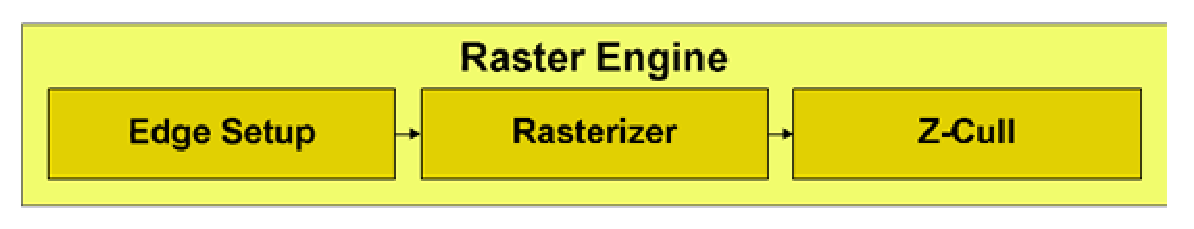
\includegraphics[height=2cm,
    angle=0]{./images/raster_engine.eps}}
\caption{Raster Engine}
\label{fig:raster_engine}
\end{figure}



\begin{framed}
  Rasterization-based techniques are mostly used in GPU to render
  graphics. The technique to provide better output is {\bf ray tracing},
  yet require much more intensively computation. Nvidia provide OptiX, a
  real-time ray tracing API on its GPU. Another project is
  OpenRT. Nvidia believe that ray tracing is the future of computer
  graphics.
\end{framed}

\section{Clock cycles and speeds}
\label{sec:clock-cycles-speeds}

The bell ring at school to tell the end of each class (say every 45 minutes), it
allows students to move from one class to another. A school is analogy to a CPU;
and a bell is in analogy to a clock pulse in a computer. Without the bell, some
class would be released early and some late. Similarly, a computer has multiple
components, each does a different work, and can be at different speed.
Periodically, a component send data along the wire to the next processing
station. To coordinate the activity, the computer uses a {\it clock pulse},
which is the crystal oscillator. Crystal oscillator is an electronic device that
create an electrical signal with a very precise frequency, typically, of
producing fixed since wave, which is then sampled to convert to hig and low
voltage.\footnote{\url{http://www.yale.edu/pclt/PCHW/clockidea.htm}}

With alternating high ('tick') and low ('tock') voltage, each tick-tock is a
{\bf cycle}, and the length (i.e. the delay from tick to tock) is often in
nanoseconds (\textcolor{red}{One nanosecond is the time for an electrical signal
to travel about one foot}), and then mapped to frequency (in Hz, MHz).
The standard external {\it clock speed} is a multiple of 33.3333...
MHz. By convention, the speed is round down to 33 MHz or 66 MHz. The other
values: 100 MHz (3x of 33.3333\ldots MHz), 133 MHz, 166 MHz or 200 MHz.
\begin{Verbatim}
    Clock   Cycle    Bus
        33Mh    30 nsec    PCI (general adapter cards)
        66Mh    15 nsec    AGP (video adapter)
        100Mh   10 nsec    mainboard clock to the CPU
        2Ghz     0.5 nsec  CPU internal clock after multipler
\end{Verbatim}
One GHz refers to one billion of times per minute the CPU's clock pulses into
the microprocessor. The clock pulse tells some circuits when to start sending data
on the wires, while it tell other circuits when the data have arived. NOTE:
\textcolor{red}{Data can be transferred at a higher frequency than the clock
rate}. With early CPUs, each has a single clock whose signal applies to CPU,
memory and all I/O devices. Modern CPUs has different clocks with different rates.
Generally, all clocks have the rate as a multiple of a given standard clock
speed as given above. An example is 
\begin{enumerate}
  \item CPU socket clock: signal generated by the mainboard to pace data
  transfer to/from CPU with memory/AGP video card/IO device. This is known as
  the standard {\it external clock speed}. The mainboard sense the CPU model
  and use the default speed
  
  The motherboard socket is the location into which the CPU processor will sit,
  which evolves over time. Two types of sockets from AMD are FM1 (using for APU
  - Chap.\ref{chap:unifying-cpu-gpu}) and AM3+ (using Bulldozer-based CPU
  and backward compatible with older CPUs). Two types of sockets from Intel are
  LGA115 and LGA2011. Older sockets from Intel are LGA1166, LGA1366.

\begin{verbatim}
Chip Type  Actual Clock  Bits/Clock  FSB  Multiplier  Speed

Pentium 4 2.4  100 MHz  4  400 MHz  24  2.4 GHz
Pentium 4 2.4A  133 MHz  4  533 MHz  18  2.4 GHz
Athlon XP 2400  133 MHz  2  266 MHz  15  2.0 GHz
\end{verbatim}  

  
  \item FSB clock: The CPU sends data, in bits, to the Northbridge chip on the
  mainboard (before going to the memory/AGP-card/IO-device) at a faster rate
  than the CPU socket clock, Fig.\ref{fig:mainboard_diagram}. 
  Thus, the CPU clock speed is
\begin{verbatim}
FSB clock speed = (actual-clock) x (transfer-rate)
\end{verbatim}
Newer CPU doesn't use FSB as there is no Northbridge between CPU and other
devices, e.g.
Athlon 64 CPU chip has its own integrated memory controller inside the CPU and a
high speed HyperTransport integrated I/O bus. 
Thus FSB clock speed would be meaningless.

\begin{mdframed}
Front Side Bus (FSB) is the external bus, shared between memory and I/O request.
With the newer generation of Intel CPU, an embeded memory controller is added,
called IMC (Integrated Memory Controller). These CPUs comes with QPI technology
(Quick Path Interconnect) (Sect.\ref{sec:QPI_IOH}). 
\end{mdframed}
  
  \item CPU clock speed: the {\it internal clock} of the CPU run at a faster
  speed than the socket clock speed, via a {\bf multiplier}
  
  \item Memory clock: the modern motherboard can generate a separate clock to
  the memory (example clock rate 100, 133, 166, and 200 MHz). DDR RAM can
  generate twice the actual clock speed (200, 266, 333, or 400 MHz).
\end{enumerate}
Due to the different clock speed, the overall performance is determined by the
slowest one. Example: The FSB run at 800 MHz, and the memory runs at 400 MHz. To
avoid this problem. The newer mainboard requires the DDR RAM should be installed
in pairs and using two separate memory busses. The memory reference is split
between the two 400 MHz buses, and producing an aggregate transfer rate 800 MHz.
\footnote{\url{http://www.yale.edu/pclt/PCHW/clockidea.htm}}

\begin{figure}[hbt]
  \centerline{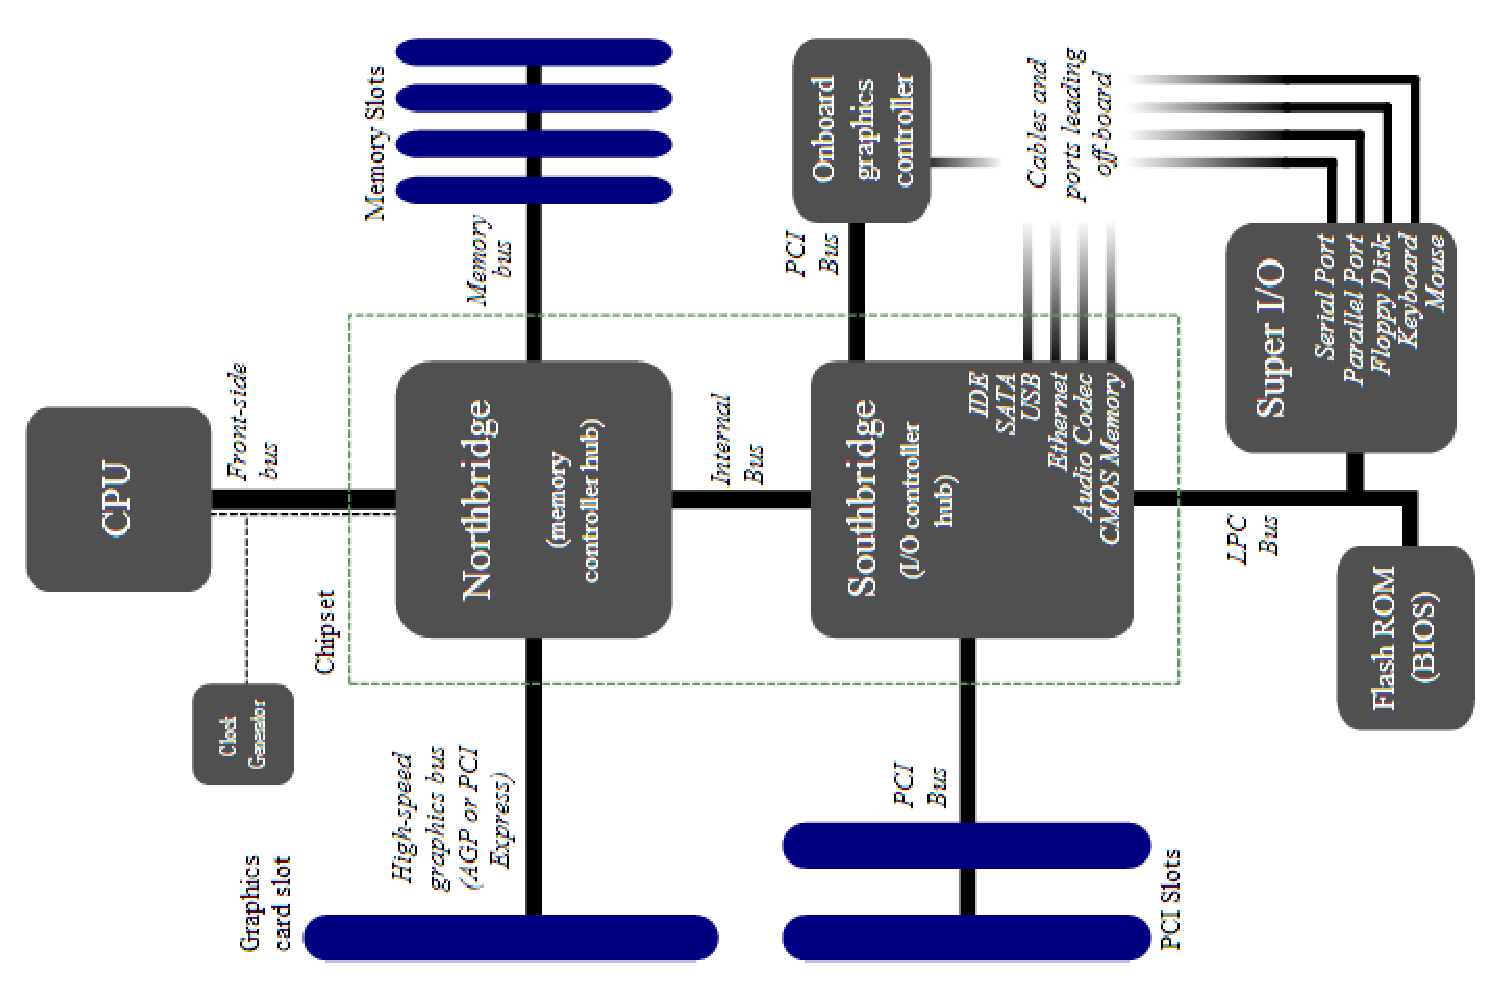
\includegraphics[height=5cm,
    angle=0]{./images/mainboard_diagram.eps}}
\caption{Connectivity between different components on a mainboard}
\label{fig:mainboard_diagram}
\end{figure}


\textcolor{red}{There are two clocks: the internal CPU clock rate and external
clock rate}.
The clock multiplier (CPU multiplier, CPU core ratio) is the speed ratio of the
internal CPU clock rate vs. the external clock rate. This is typically fixed
during manufacturing. Some motherboards has the option to change using BIOS
setup (OverClock section, e.g. CPU core (Non-Turbo) ratio) which makes the CPU
run faster (TUAN)
\begin{itemize}
  \item Intel 2.4 Pentium 4: with a 100 MHz
internal clock speed, data is transferred at 4x per clock tick, then the I/O
(front-side-bus FSB to memory) is 400 MHz. The CPU has a 'multiplier' of 24,
the internal clock rate is 24x100 = 2.4 GHz.

  \item Intel 2.4A Pentium 3: with 133 MHz internal clock speed, the Front-Side
  Bus is 533 MHz. Using the multiplier of 18, then the internal clock rate is
  18x133 = 2.4 GHz.
\end{itemize}
Newer Intel and AMD CPUs use a new technology that doesn't limit the clock speed
to standard values (Intel Turbo Boost, AMD Turbo Core). This enables the
processor to run at a higher speed automatically, i.e. no need to adjust BIOS
setting, for a short period of time. Example: a 3.3GHz Core i7-3960X Extreme
Edition can run at 3.9 GHz.

\begin{mdframed}
To improve the CPU
\begin{enumerate}
  \item faster clock speed: reduce the time for each class and student need to
  learn faster
  
  \item build a pipeline: instead of using 45-min class, break down into 15-min
  class, as some 45-min class doesn't use all 45-min.
  
  \item parallelism: add more classrom. Only works if the school has more
  students, i.e. the CPU has more data
  
  \item class size: double the number of students in each class room (only if
  there are more students studying the same course), e.g.  from 32-bit to 64-bit
  data-oriented operation 

  
  \item build another school: use multi-core architecture
   
\end{enumerate}
The first option is the easiest; however it soon reaches the limit. In 2004,
Intel reached the almost limit, 3 GHz. AMD even though has lower clock rate 2
GHz, it has more parallelism (first switching to 64-bit), and thus is still as
much powerful as Intel chip.  Then, multi-core is added
(Sect.\ref{sec:core-thread}). 

\end{mdframed}

The GPU chip is a processor just like a CPU on the mainboard. The videocard,
e.g. GTX560 is where the GPU chip reside. So GTX 560 is not a GPU, it's a
videocard. The details is given in Fig.\ref{fig:GPU_videocard}.


\begin{figure}[hbt]
  \centerline{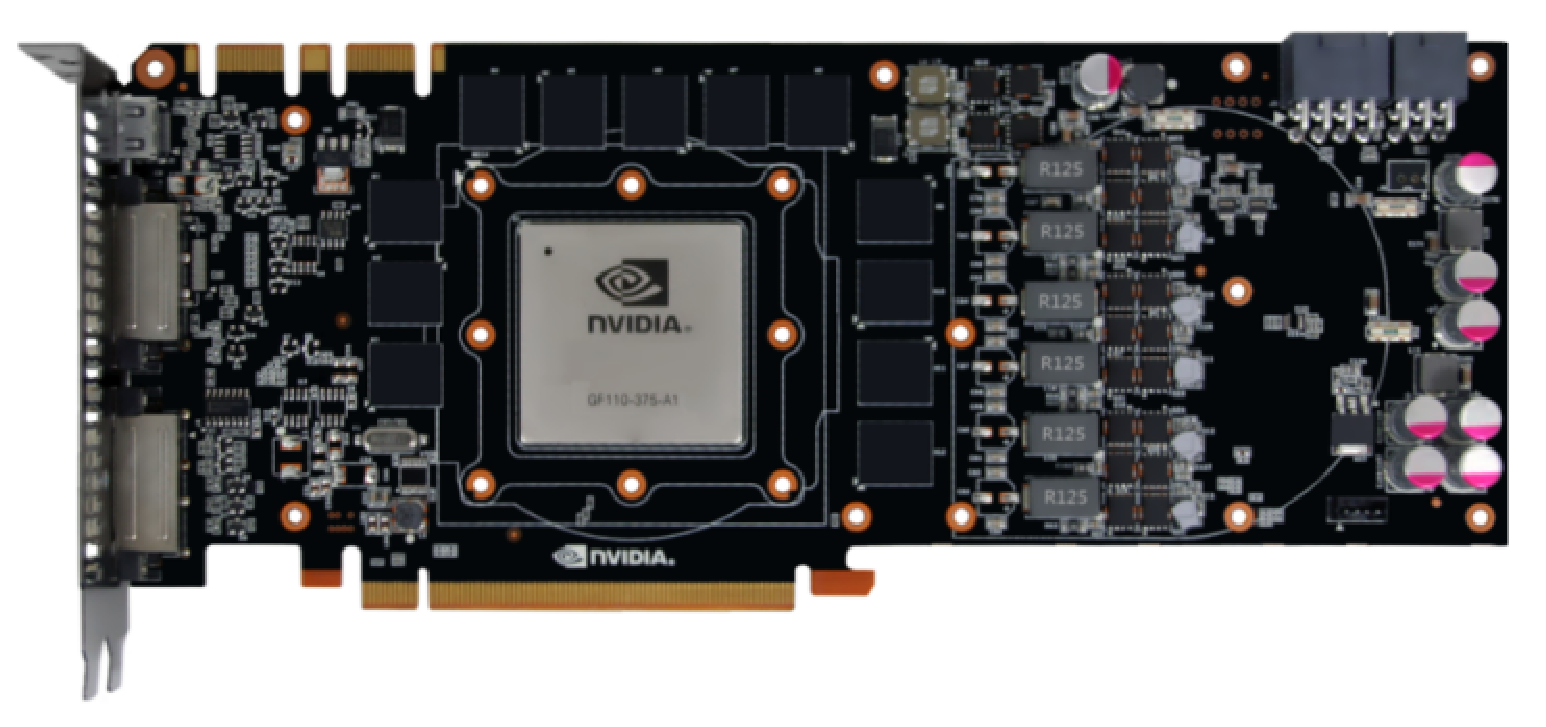
\includegraphics[height=8cm,
    angle=0]{./images/GPU_videocard.eps}}
\caption{GTX580 videocard: The large NVIDIA chip is the GPU chip (here is
GH110). The 12 smaller ships surrounding it is the video RAM chips (which is
GDDR5 in this case). The bus connection between one RAM chip with the
GPU chip is 64-bit. , i.e. total 64x6=384 bits}
\label{fig:GPU_videocard}
\end{figure}


On Nvidia GPU, there are 3 ``clocks'', corresponding to speed of core clock,
shader clock (graphics clock), and memory access (memory clock). 
\begin{itemize}
  \item {\bf Memory clock}: How many times a memory access per second.
  %The speed of the GPU defined in terms of this

\item With unified architecture, each GPU core can handle any tasks. However,
depending on the task it does (i.e. general purpose computation or graphical
processing), the GPU core can run at different clocks. If  it does shading, the
clock is {\it shader clock} (or graphics clock). If it does general-computing,
the clock is {\it core clock}.

ATI set the speed of {\bf core clocks} and {\bf shader clocks}  the same.
However, Nvidia set them different (core clock (processor clock) is 2x shader
clock), until Kepler architecture (Chap.\ref{chap:Kepler}). Nevertheless, it
doesn't mean core and shaders are different, it just the GPU cores run at
different speeds when doing different things.
\end{itemize}

\begin{verbatim}
# of ROPs x Core Clock = Pixel Fill Rate
\end{verbatim}
Example: GTX 470: 40 x 607.5 MHz = 24.30 GPixel/s. So GTX 475 with 32 raster
operators to have the same performance, it needs a higher clock, e.g. 32 x 760
MHz = 24.32 GPixel/s.


\begin{framed}
\textcolor{red}{The core clock runs some functions on the 
multiprocessor level},  like the instruction decoder or control logic or storage
arrays, and  \textcolor{red}{the shader clock runs the individual processors}. The
shader clock is thus the fastest of the two, and this sets the speed
of arithmetic operations by the processor. Shader clock is 2.5x the
core clock (see Clock rate on Hardware specification).
The term ``hot clock'' refers to the fastest clock - the shader clock. Shader
clock was introduced in G80 Tesla-architecture GPU and was used in Tesla- and
Fermi-architecture GPUs.
\end{framed}

\textcolor{blue}{Since GF100, {\bf core clock} concept is no longer present} as
everythings tights to the shader clock (graphics clock). Only the ROPs and L2
cache operate on a separate clock domain. Everything else runs at a derivative
of the shader clock. The execution hardware runs at the full shader clock speed,
while the texture units, PolyMorph and Raster Engines all run at 1/2 shader
clock speed.

\section{Error Correcting Code (ECC)}
\label{sec:ECC}


\textcolor{red}{ECC in GDDR5}:
GK110 Kepler GPUs offered ECC protection for GDDR5 by allocating some of the
available memory for explicit ECC storage. 6.25\% of the overall GDDR5 is
reserved for ECC bits.
The register files, shared memories, L1 cache, L2 cache, and the GDDR5 are
protected by a Single‐Error Correct Double‐Error Detect (SECDED) ECC code.


In the case of a 12 GB Tesla K40 (for example), 750 MB of its total memory was
reserved for ECC operation, resulting in 11.25 GB (out of 12 GB) of available
memory with ECC turned on for Tesla K40.

Also, accessing ECC bits caused a decrease in memory bandwidth of 12-15\% on
typical workloads, compared to the non-ECC case.

\textcolor{red}{ECC in HBM2}:
Since HBM2 supports ECC natively, Tesla P100 does not suffer from the capacity
overhead, and ECC can be active at all times without a bandwidth penalty.





\section{Memory architecture}
\label{sec:close-view-at}

\subsubsection{G80/G92}
\label{sec:g80g92_memory}

Let's briefly review G80/G92
architecture\footnote{\url{http://alasir.com/articles/Nvidia_fermi_architecture/}}:
it has 8 clusters (TPCs), each with 2 subclusters (SMs). Each SM has 8
pipelines SIMD (SPs).  In terms of memory, each SM has
\begin{itemize}
\item register unit with a {\it 8K 32-bit register files}
\item {\it 16KB user-managed shared memory per subcluster} shared
  equally to all SPs,
  \textcolor{red}{each SP has 2KB of shared memory to use}.
\end{itemize}
There are 2 types of read-only cache memory: cache constant (64KB
total, i.e. 8KB per cluster), L1 texture cache (128KB total, i.e. 16KB
per cluster).

With six 64-bit memory controllers (channels), G80 has 384-bit
bandwidth. Each channel (or raster partition) has 4 ROPs, i.e. 24 ROPs
in total. G92 has only four 64-bit memory channels, i.e. 256-bit
bandwidth.

\begin{itemize}
\item G90/G92 use a companion chip called NVIO to provide output
  interfaces (two RAMDACs, two DVI/HDMI transmitters, one legacy
  TV-out)
\item G80 use PCI Express v1.0, while G92 use PCI Express v2.0
\end{itemize}

\subsubsection{GT200}
\label{sec:gt200}

Let's briefly review GT200
architecture\footnote{\url{http://alasir.com/articles/Nvidia_fermi_architecture/gt200_gt300_architecture.shtml}}:
it has 10 clusters (TPCs), each with 3 subclusters (SMs). Each SM has
8 pipelines SIMD (SPs).  In terms of memory, each SM has
\begin{itemize}
\item register unit with a {\it 16K 32-bit register files}

\item {\it 24KB shared memory per subcluster} shared equally to all
  SPs, i.e.  \textcolor{red}{each SP has 3KB of shared memory to use}.
\end{itemize}
There are 2 types of read-only cache memory: cache constant (64KB
total, i.e. 8KB per cluster), L1 texture cache (128KB total, i.e. 16KB
per cluster).  GT200 has eight 64-bit memory channels, i.e. 512-bit
bandwidth. Each channel work with 4 ROPs, i.e. 32 ROPs in total.

\begin{figure}[hbt]
  \centerline{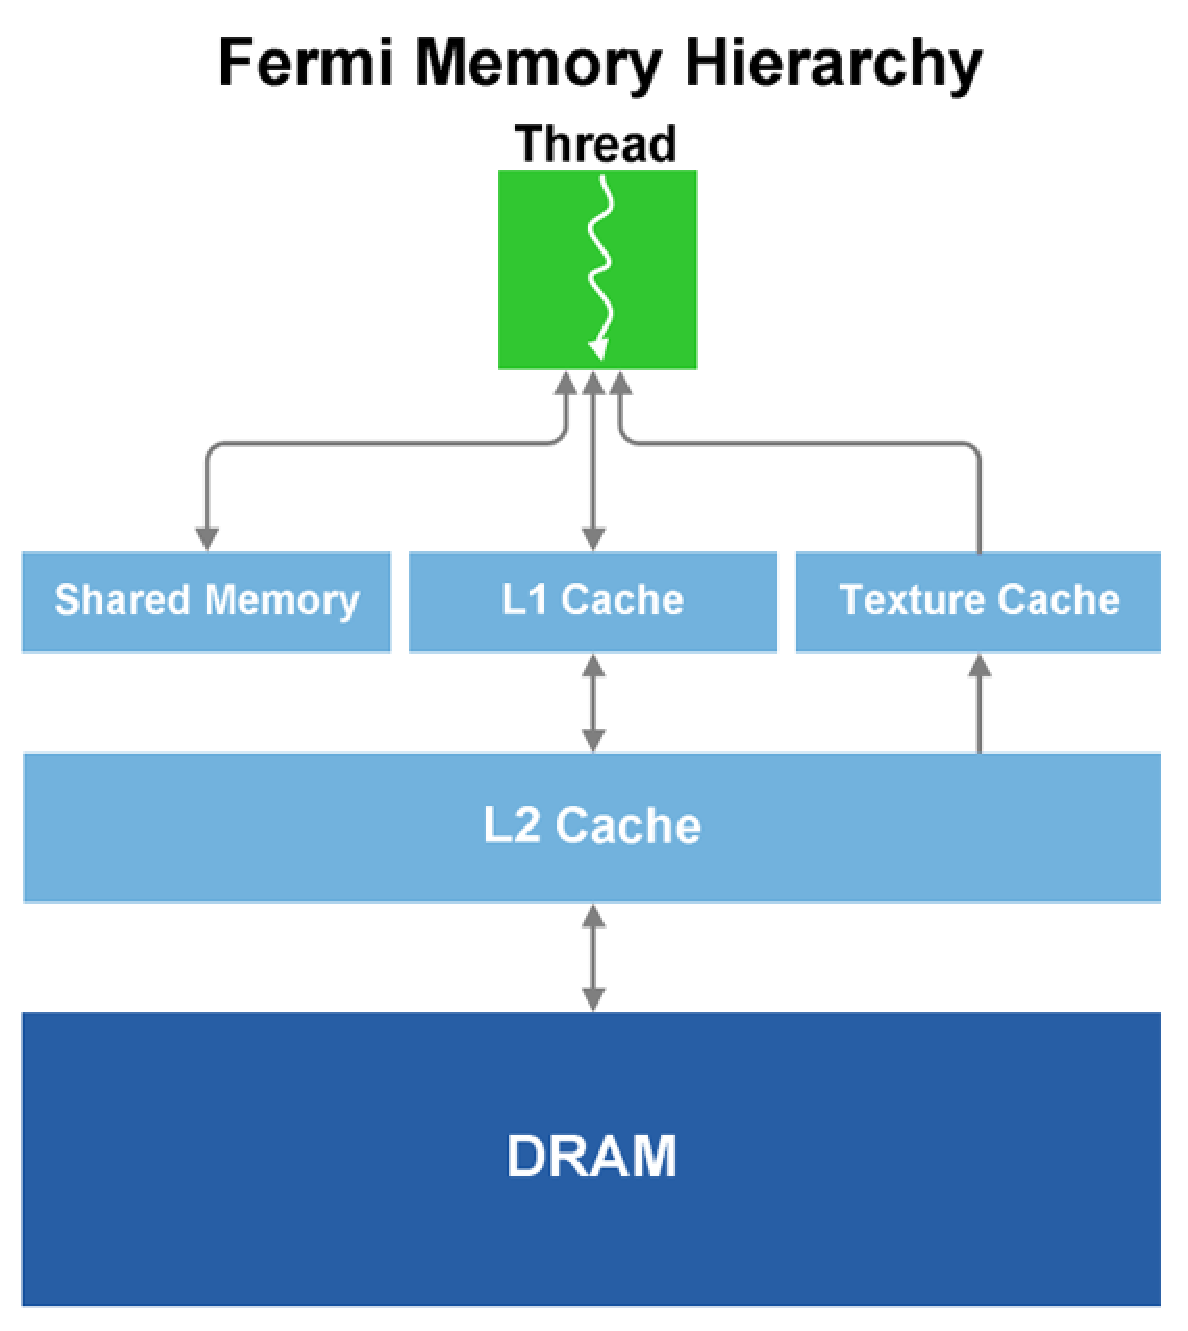
\includegraphics[height=5cm,
    angle=0]{./images/fermi_memory1.eps}}
  \caption{Fermi memory hierarchy}
  \label{fig:fermi_memory}
\end{figure}

\subsubsection{Fermi (GF100)}
\label{sec:fermi-gf100}

In Fermi, each subcluster has a local (fast) 64KB memory configurable
into shared memory ({\it software managed}) vs. L1-cache
({\it hardware managed}) in either 48KB shared memory and 16KB L1
cache, or 16KB shared memory and 48KB L1
cache\footnote{some applications have threads access the off-chip data
  more often than sharing the result data, i.e. it can increase
  performance if the data is cached; such applications need more cache
  than shared memory. Thus the configurable memory balances between
  the two application purposes},
as shown in Fig.~\ref{fig:fermi_memory}.

\begin{framed}
  Nvidia says that 64-bit instructions use all the register access
  resources, which means the dual-issue mode not compatible with double
  precision. We don't however know if, in terms of implementation, a
  single SIMD handles all operations on doubles or if 2 SIMDs run
  together at half speed, as Nvidia wouldn't give any specifics on
  this\footnote{\url{http://www.behardware.com/articles/772-6/Nvidia-fermi-the-gpu-computing-revolution.html}}.
\end{framed}

GF100 have the L2-cache memory of 768KB, i.e.  128KB of such cache per
memory controller.  This L2 cache is shared by all SM to serve all
memory controller load/store/texture requests, i.e. 48KB per SM. It
also help by caching temporary register spills of complex
programs\footnote{when the data in thread is large and the limit of
  registers, the registers for a thread may not hold all; thus
  prior-Fermi GPU need to spill them to DRAM which greatly decrease
  the performance. Now, with Fermi, it can be avoided by caching to L2
  cache. In addition, L1 cache can be used as temporary register
  usage.}
Thus, any L2 write from any cluster are visible in the next clock to
any other cluster in the chip.
\textcolor{red}{Data in L2 cache are alive between kernel calls; but
  not guarantee with L1 and not with register files.}

\begin{framed}
  In Tesla 2nd gen, shared memory is used to share data between
  threads in the same thread-block (mainly in parallel algorithms);
  data between thread-blocks need to share via the device global
  memory. Since Fermi, data in L2 cache is an alternative for sharing
  data between thread-blocks.
\end{framed}

In Fermi, register files and shared memory do not run on the fast
clock, but on the core clock. So between the register file and the
shared memory, there must be a total of 80 inputs and 32 outputs
available - an aggregate of 112 ports across all the storage array. Of
course, a couple of other units use the register files as well -
prominently the texturing unit and load store pipelines, so the total
is probably closer to 128.


\subsection{G80/G92}
\label{sec:g80g92-architecture}

A pixel is a vector of 4 components (RGBA - red,green,blue,alpha) or
also named as XYZW since they doesn't necessarily represent color
information. These 4 components are processed in parallel.

At each clock cycle, a single instruction is issued to operate on 4 pixels.
However, it often happens that an instruction isn't applied to all components,
i.e. each component use a different operation. Thus, to avoid wasting resources,
AMD/ATI shaders cores are capable of simultaneously processing 2 instructions.
\begin{verbatim}
MUL R1.xy
ADD R1.z
\end{verbatim}
This is know as ``co-issued'' or multiple-instructions multiple-data
(MIMD). However, in Nvidia, the cores are SIMD. The major difference
is that instead of processing 4 pixels of 4 components per cycle, the
scalar processor processes 1 component of 16 pixels. In G80 chips -
Nvidia's first unified architecture, the first generation of unified
shader only supports one component at a time, i.e. scalar, and thus
given the name {\bf scalar processors} (SP), and later named {\bf streaming 
processor} (SP).

\begin{figure}[hbt]
  \centerline{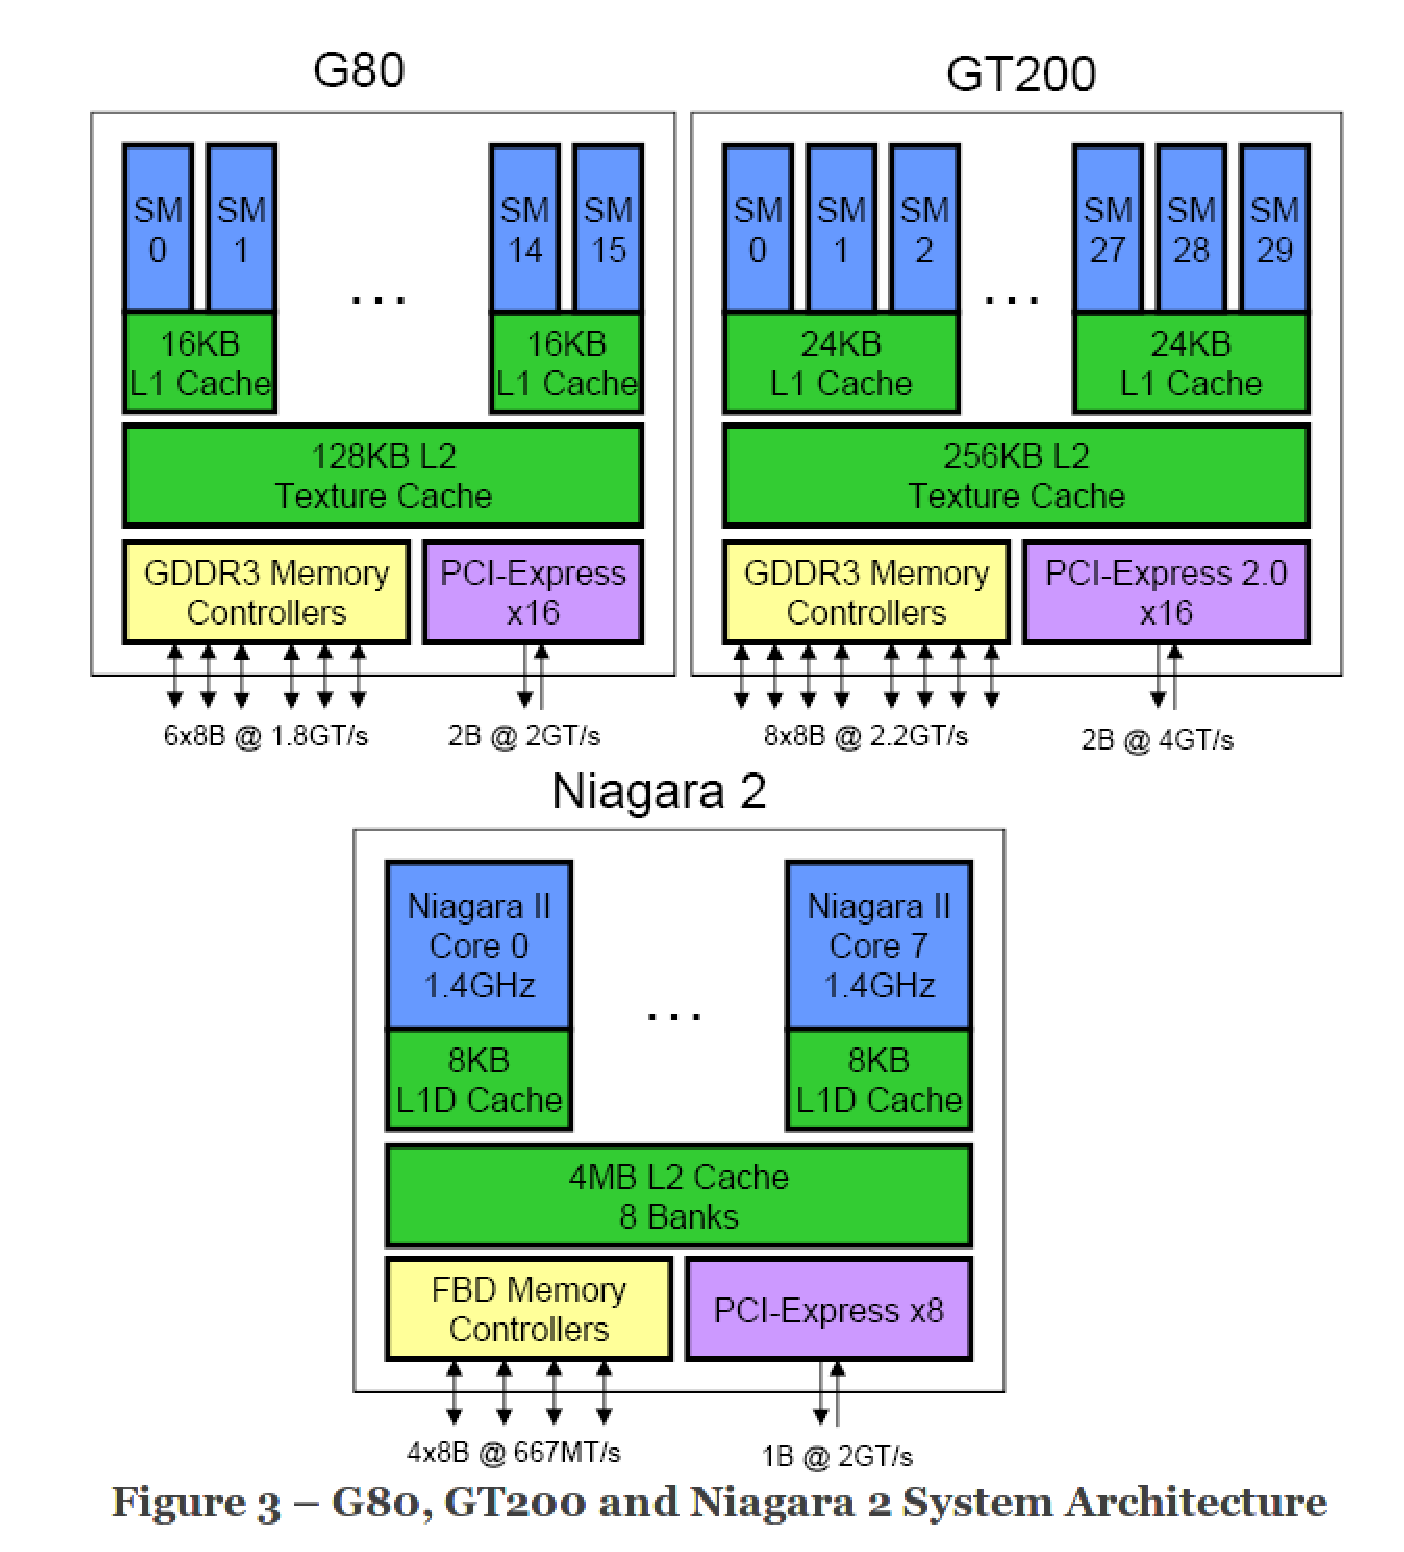
\includegraphics[height=10cm,
    angle=0]{./images/g80_gt200_niagra.eps}}
\caption{G80, GT200 and Sun Niagra 2}
\label{fig:g80_gt200_niagra}
\end{figure}



\begin{itemize}
\item GeForce 7: one instruction for a single component of 16 pixels
  take \textcolor{red}{4 clock cycles}
\item GeForce 8: one instruction for a single component of 16 pixels
  take \textcolor{red}{3 clock cycles}. A 25\% improvement due to the
  reorganization of MUL R1.xy into 2 separate MUL R1.x and MUL R1.y.
\end{itemize}
However, SPs can only do simple arithmetic operations (MAD/MUL),
e.g. 32-bit floating-point multiply-add (MAD) operation or 32-bit
integer addition or 24-bit integer multiplication),
Fig.~\ref{fig:unified_shader}. A separate unit, known as special functional unit
(SFU), is required to do complicated functions (EXP, LOG, RCP, RSQ, SIN, COS);
each one needs \textcolor{red}{4 clock cycles} to complete.

\begin{figure}[hbt]
  \centerline{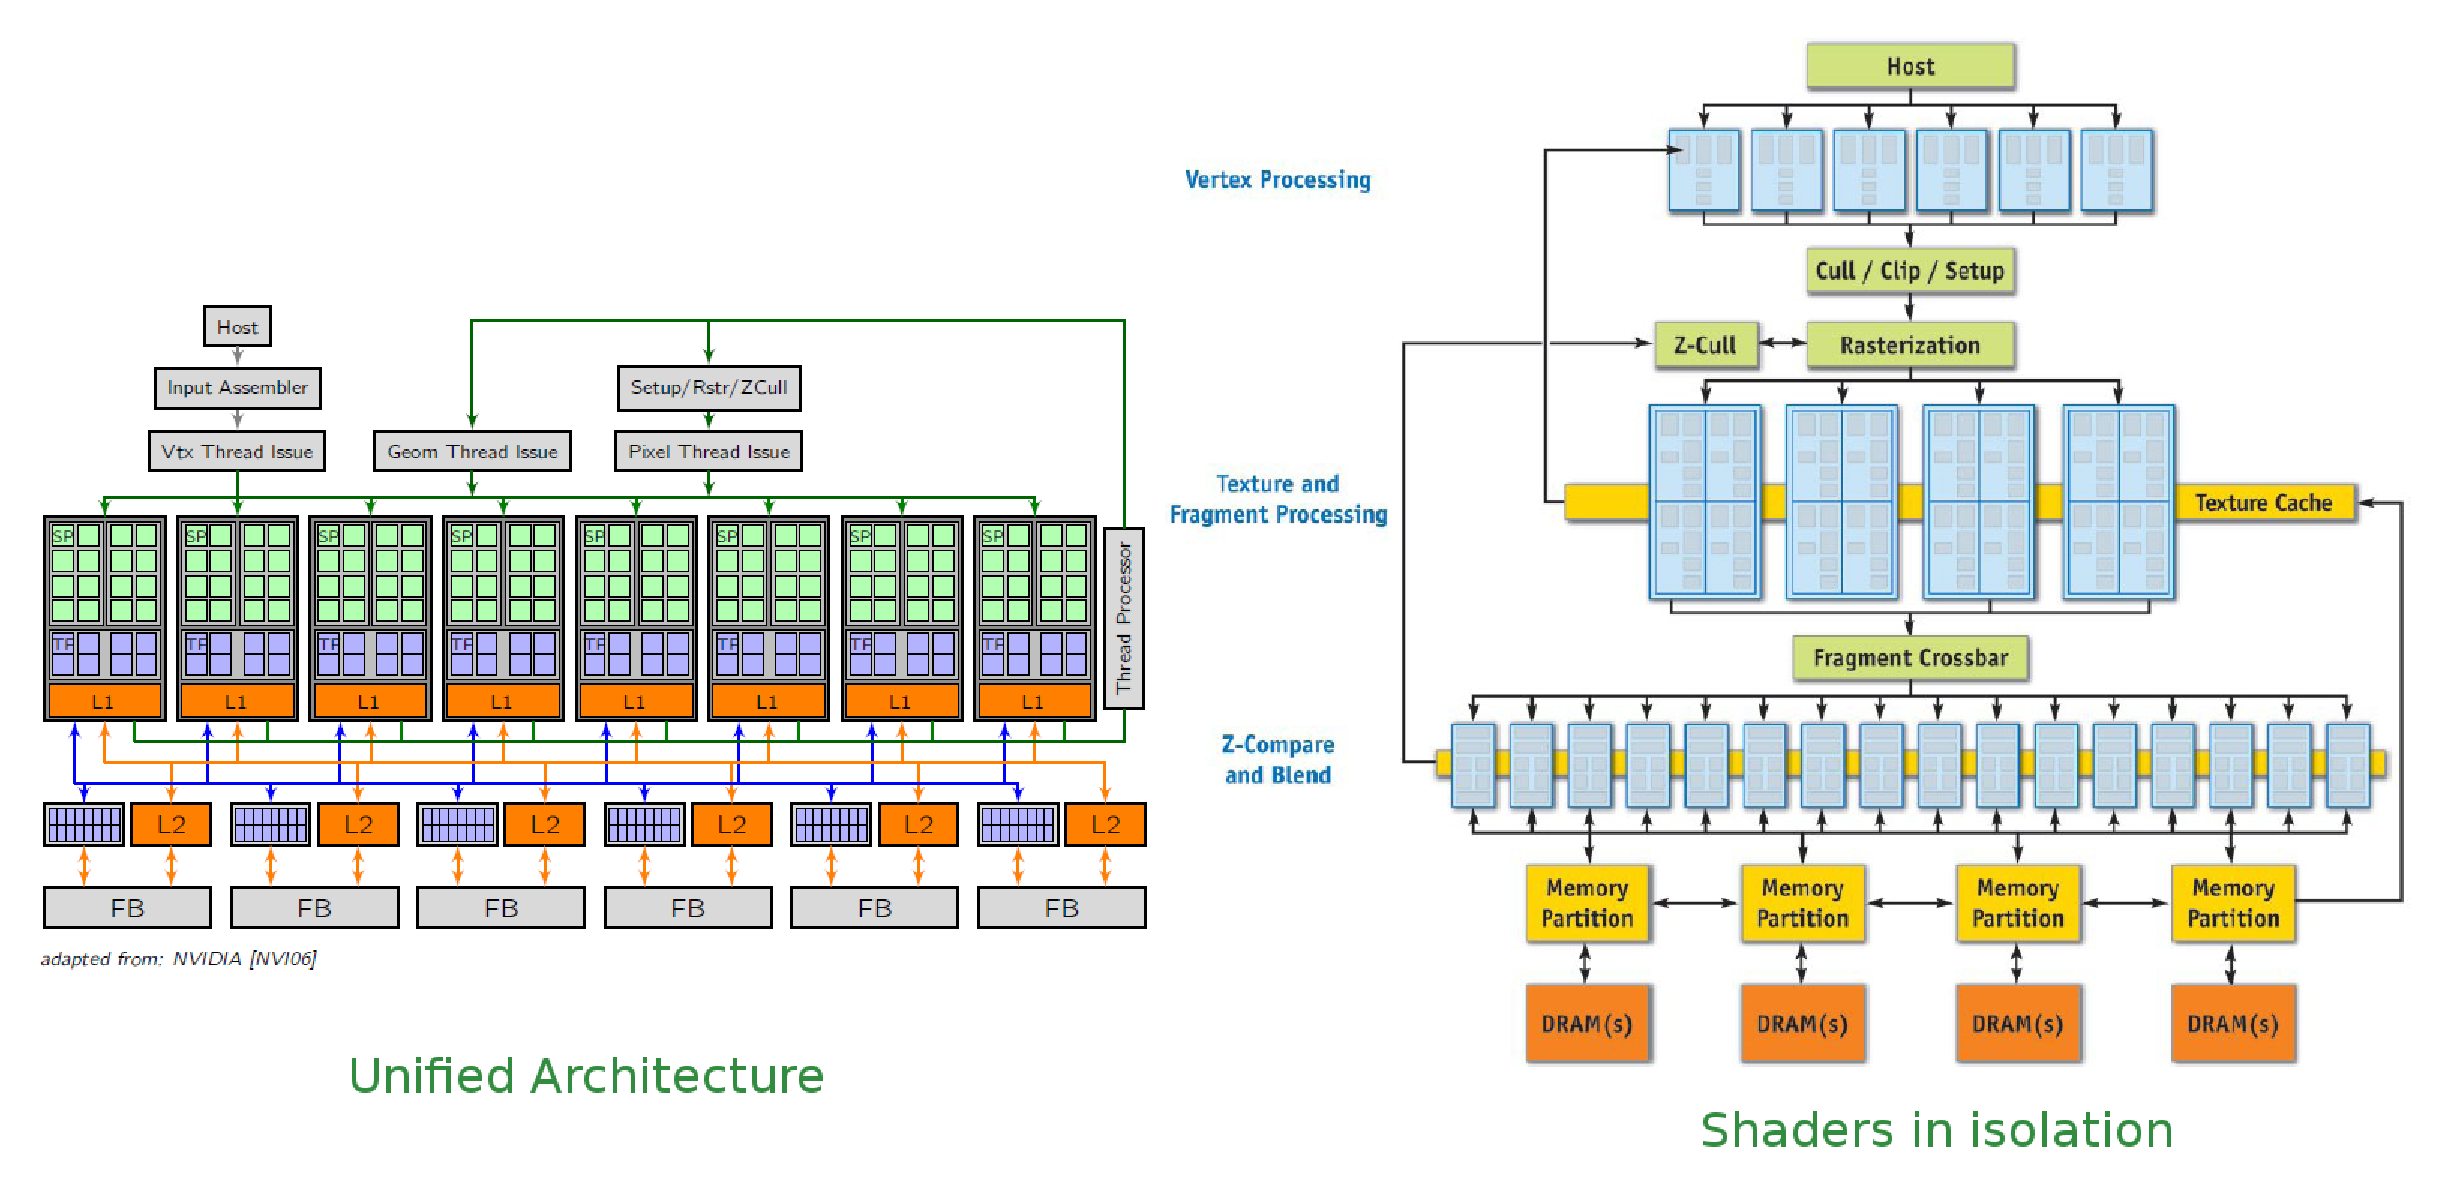
\includegraphics[height=7cm, angle=0]{./images/unified_shaders.eps}}
  \caption{(A) Unified shaders (GeForce 8800); (B) shaders in separate
    (GeForce 6)}
  \label{fig:unified_shader}
\end{figure}

\begin{framed}
  In graphical applications, the speed is more important than the
  precision. So, in G80's chips and earlier, all execution units in
  GPU support only 32-bit operations and don't support 64-bit
  operations. Newer GPU architectures have better support for double-precision
  calculations.
\end{framed}

As you see, a single SP is indeed a quite simple architecture. Nvidia creates a
complete processor, called a {\bf streaming multiprocessor} (SM), by using: 8
SPs, 2 special functional units (SFUs) + 1 multithread instruction fetch and
issue unit (MT issue) + an instruction cache (I cache) + a read-only constant
cache (C-cache) + 16KB read/write shared memory.

At a higher level, 2 SMs, combined with one {\it texture unit} (texture memory
unit TMU) \footnote{texture unit (or texture pipe) to serve 2 SMs to
  balance the expected ratio of math operations to texture operations}
+ one geometry controller (i.e. PolyMorph unit) + one shared-memory
controller (SMC), form a {\bf Thread Processor Cluster} (TPC). All
TPCs, along with L2 texture cache, form the
{\bf Streaming Processor Array} (SPA).

\begin{figure}[hbt]
  \centerline{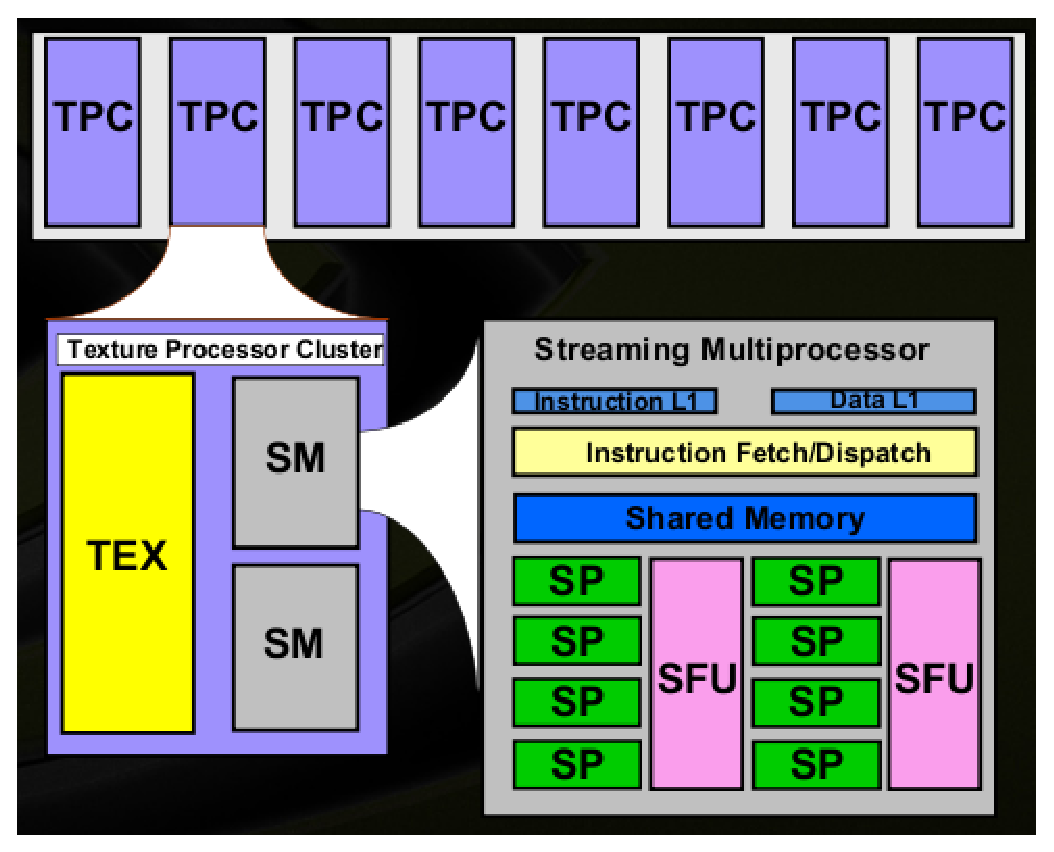
\includegraphics[height=5cm,
    angle=0]{./images/G80_chip.eps}}
  \caption{SPA, TPC, SM, SP in G80}
  \label{fig:G80_chip}
\end{figure}

G80, with 128 processors, has 8 TPCs, Fig.~\ref{fig:G80_chip}.  To
form a complete graphics chip, we still need one execution unit in
GPU, known as a fixed-function {\it raster operation processor} (ROP)
that do the final work of by generating a raster
picture\footnote{\url{http://en.wikipedia.org/wiki/Raster_graphics}}
by writing batches of fragments to framebuffer (FB) memory to display
on the monitor
\footnote{\url{http://ixbtlabs.com/articles3/video/cuda-1-p3.html}}.
In G80s chip, there are 6 ROP partition and six 64-bit FB memory
controllers (i.e. $6\times 64=384$-bit bandwidth). Each ROP partition
has 4 ROP units, i.e. G80s chip has 24 ROP units.


The input information, i.e. color and depth values, are transferred
via an interconnection network. This network also routes the texture
memory read requests from SMs to DRAM and read data from DRAM through
L2 texture cache back to SMs.  The input of the SMs is the coordinate
information of the pixel/vertex, then does the computation to find the
color\footnote{\url{http://www.realworldtech.com/page.cfm?ArticleID=RWT090808195242&p=10}}.

\begin{framed}
  In CUDA, SMs can process vertex, geometry, and pixel-fragment shader
  programs and parallel computing functions (kernels).
\end{framed}

\subsection{GT200 (T10 architecture)}
\label{sec:gt200-1}

The major changes are, as shown in Fig.\ref{fig:T10_arch}(A)
\begin{enumerate}
\item second generation SP use 55nm technology $\rightarrow$ more SPs
  (from 128 to 240), i.e. 10 TPC, each TPC has 3SMs

\item second generation SM: add one 64-bit arithmetic unit (to process
  double-precision) per SM, i.e. DP-based computation is 1/8 of
  SP-based computation in performance. With DP support, and running at 
  1.3GHz, it can do 1 TFLOP SP, and 86.4 GFLOP DP.
\item Each TPC is 3 SMs, rather than 2. 
\item Faster bandwidth, use 512-bit interface, i.e. 102GB/s bandwidth.

\end{enumerate}

\begin{figure}[hbt]
  \centerline{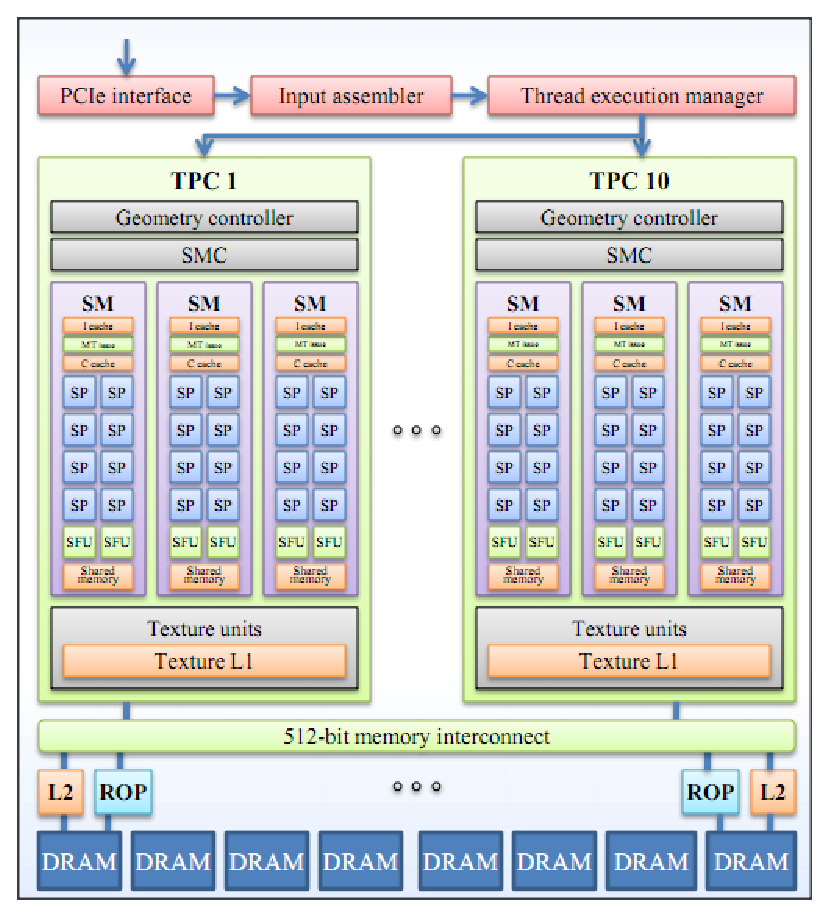
\includegraphics[height=5cm,
    angle=0]{./images/T10_Tesla.eps}; 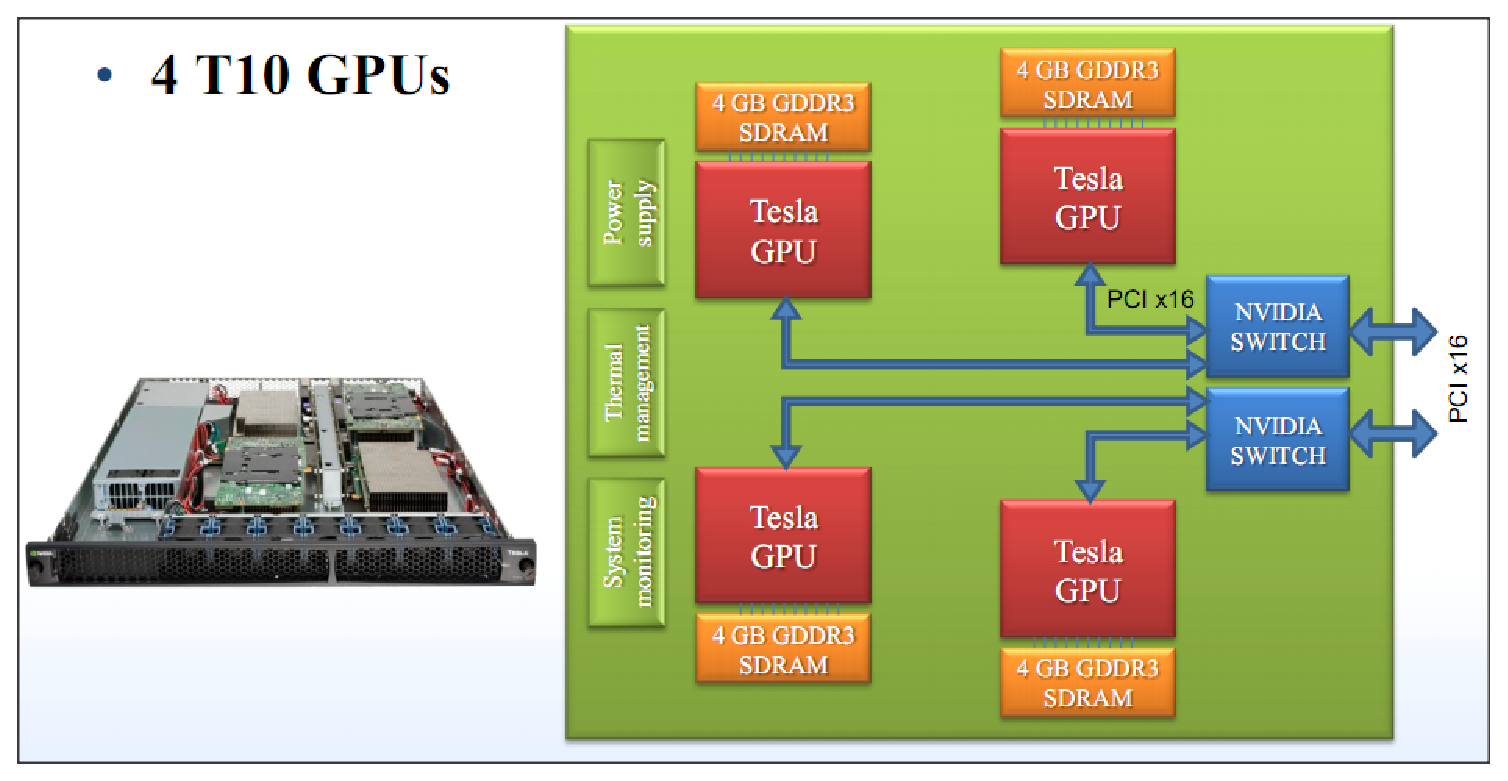
\includegraphics[height=5cm,
    angle=0]{./images/S1070.eps}}
\caption{(A) T10 architecture (GT200); (B) S1070 GPU Computing Server}
\label{fig:T10_arch}
\end{figure}

S1070 is the device with 4 chip T10, connecting to the system with 2 PCIe-x16
bus. Each two T10 chips connect to one PICe-x16 using an Nvidia switch,
Fig.\ref{fig:T10_arch}(B).
% Fig.\ref{fig:S1070}.
% 
% \begin{figure}[hbt]
%   \centerline{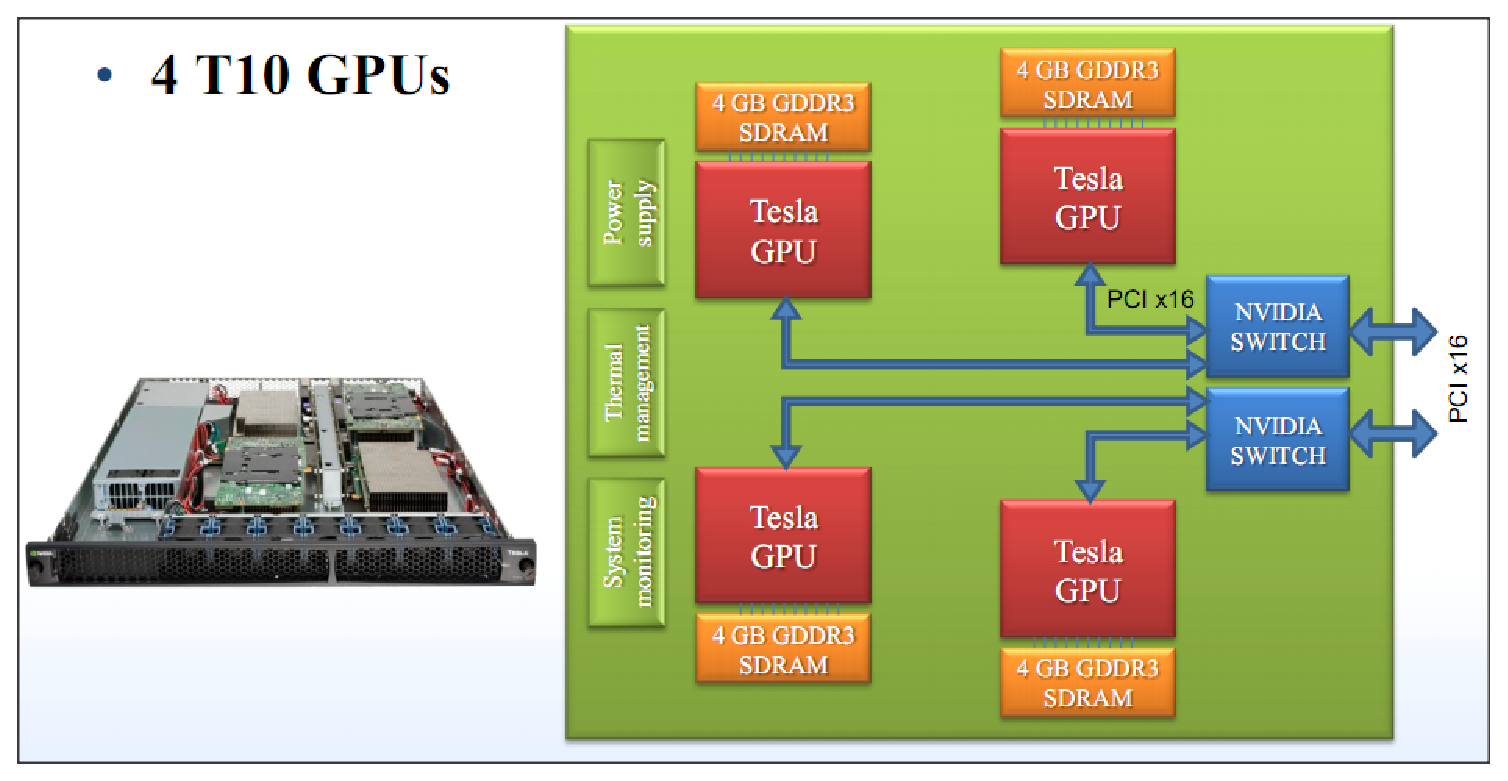
\includegraphics[height=5cm,
%     angle=0]{./images/S1070.eps}}
% \caption{S1070 GPU Computing Server}
% \label{fig:S1070}
% \end{figure}

\section{Tesla 3 (Fermi) GPU}

Tesla 3 (widely known as Fermi) is C2050 which use GF100 chip.

\subsection{GF100 (Fermi)}
\label{sec:gf100-fermi}

SUMMARY: GF100 uses memory interface    320-bits; memory bandwidth 133.9 GB/s;
core clock 607.5 MHz and processor    clock 1215 MHz while memory clock 837MHz (3348 MHz
effective data rate).    GRAPHICS: 56 texture units; 40 raster operators (ROP);
texture fill rate 34    billion/sec; pixel fill rate: 24.28 GPixel/s; 3-way SLI
support.


\begin{figure}[hbt]
  \centerline{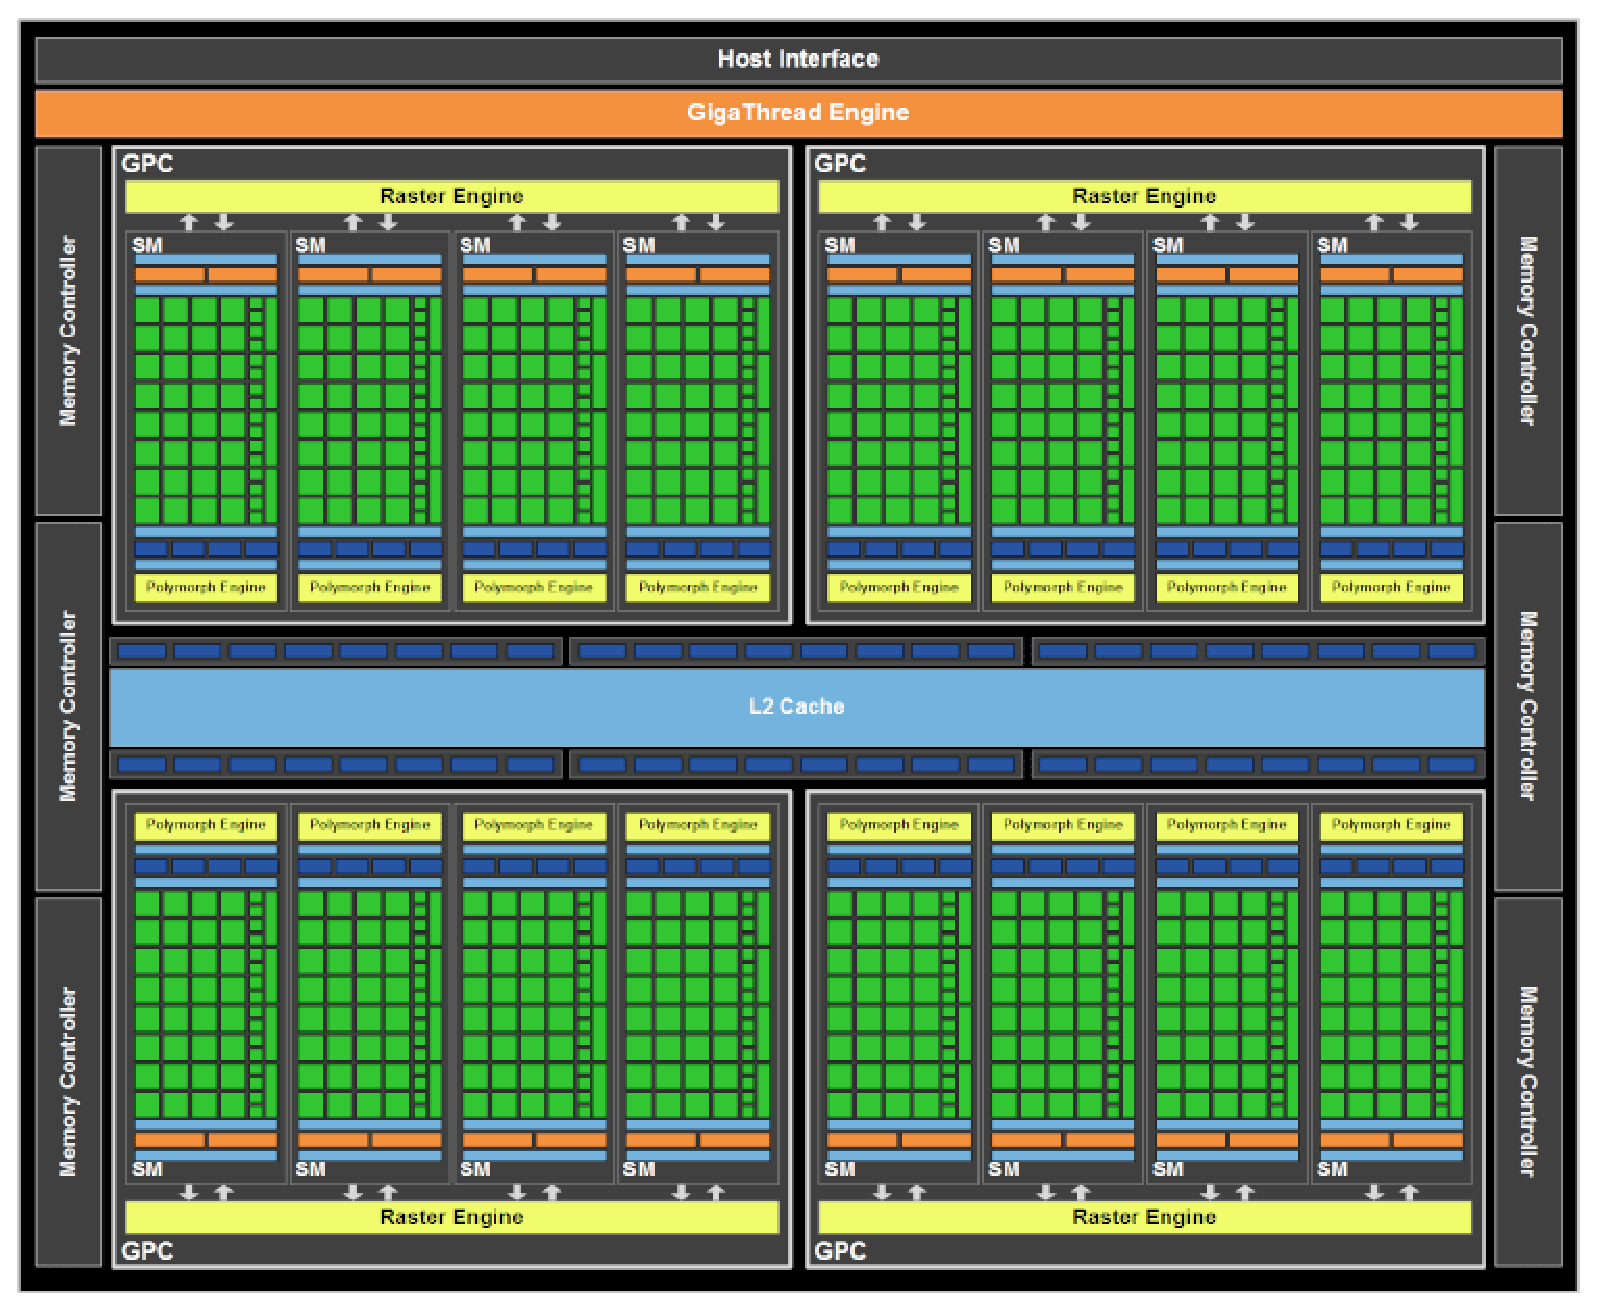
\includegraphics[height=7cm,
    angle=0]{./images/gf100.eps}; 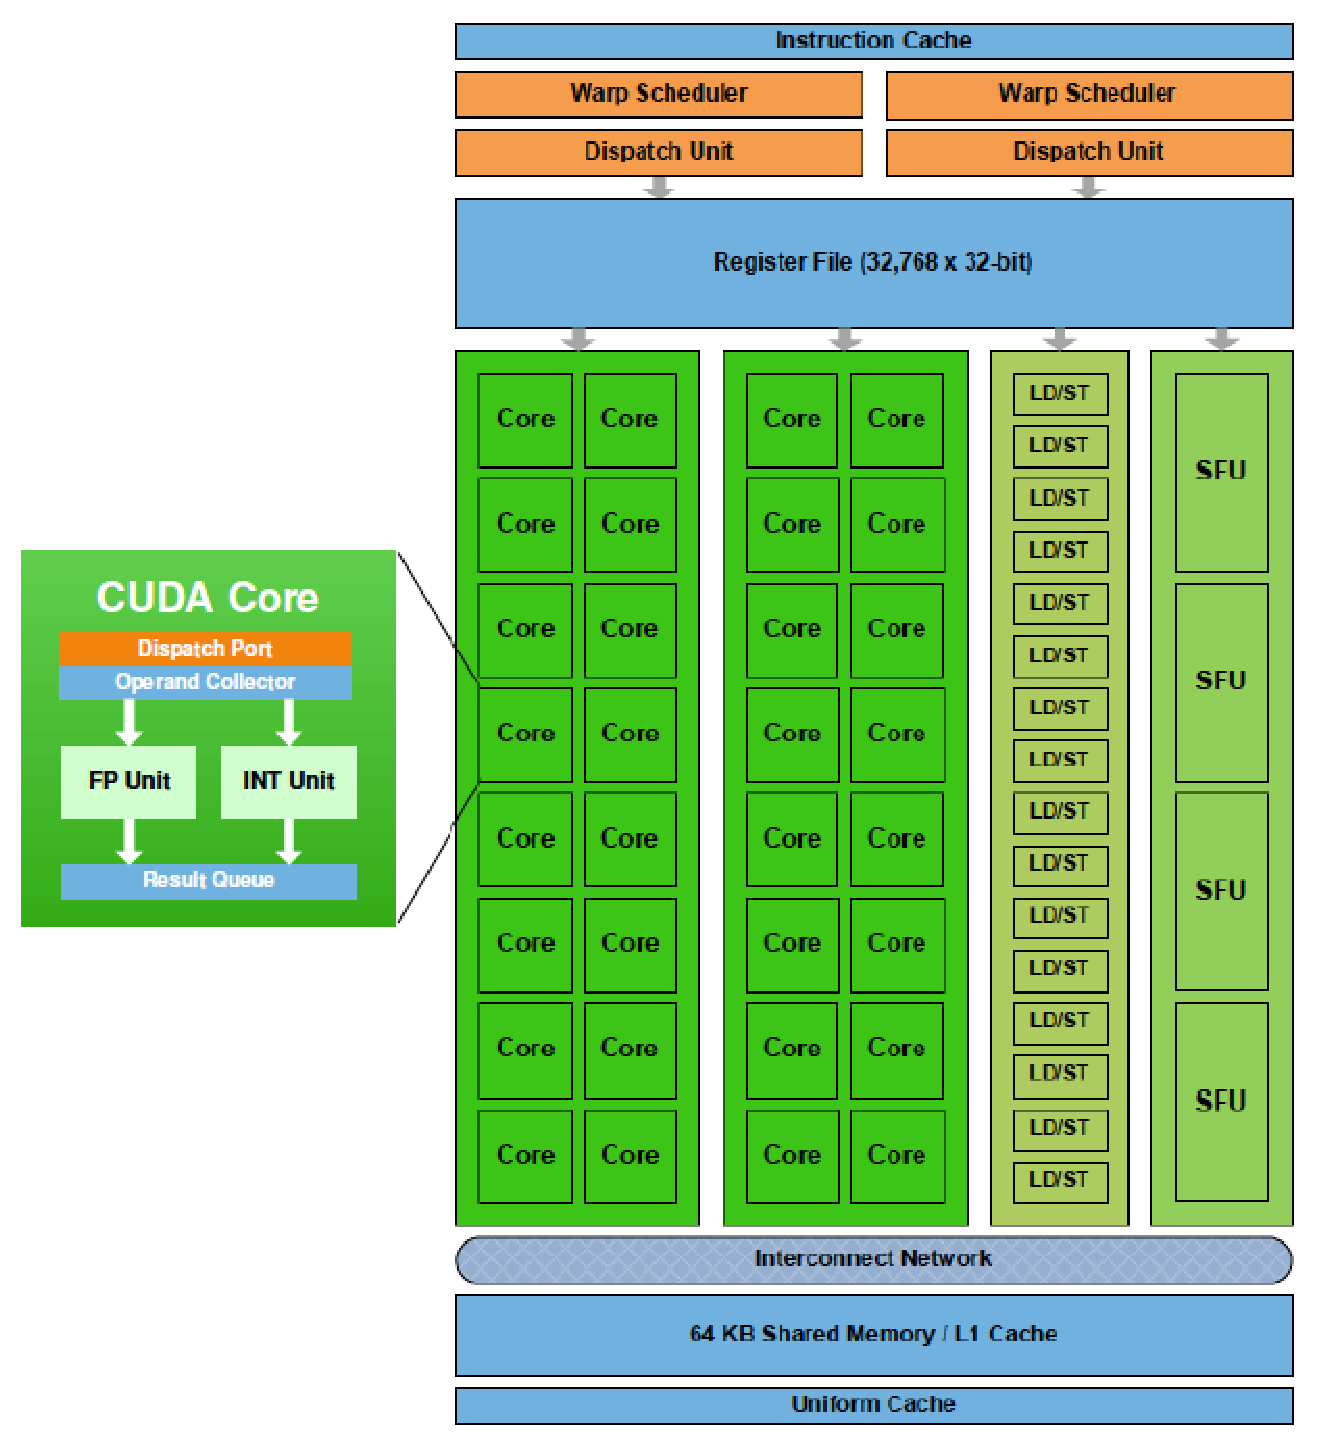
\includegraphics[height=7cm,
    angle=0]{./images/gf100_sm.eps}}
\caption{(A) Diagram of GF100 chip; (B) An SM in GF100}
\label{fig:gf100}
\end{figure}

% \begin{figure}[hbt]
%   \centerline{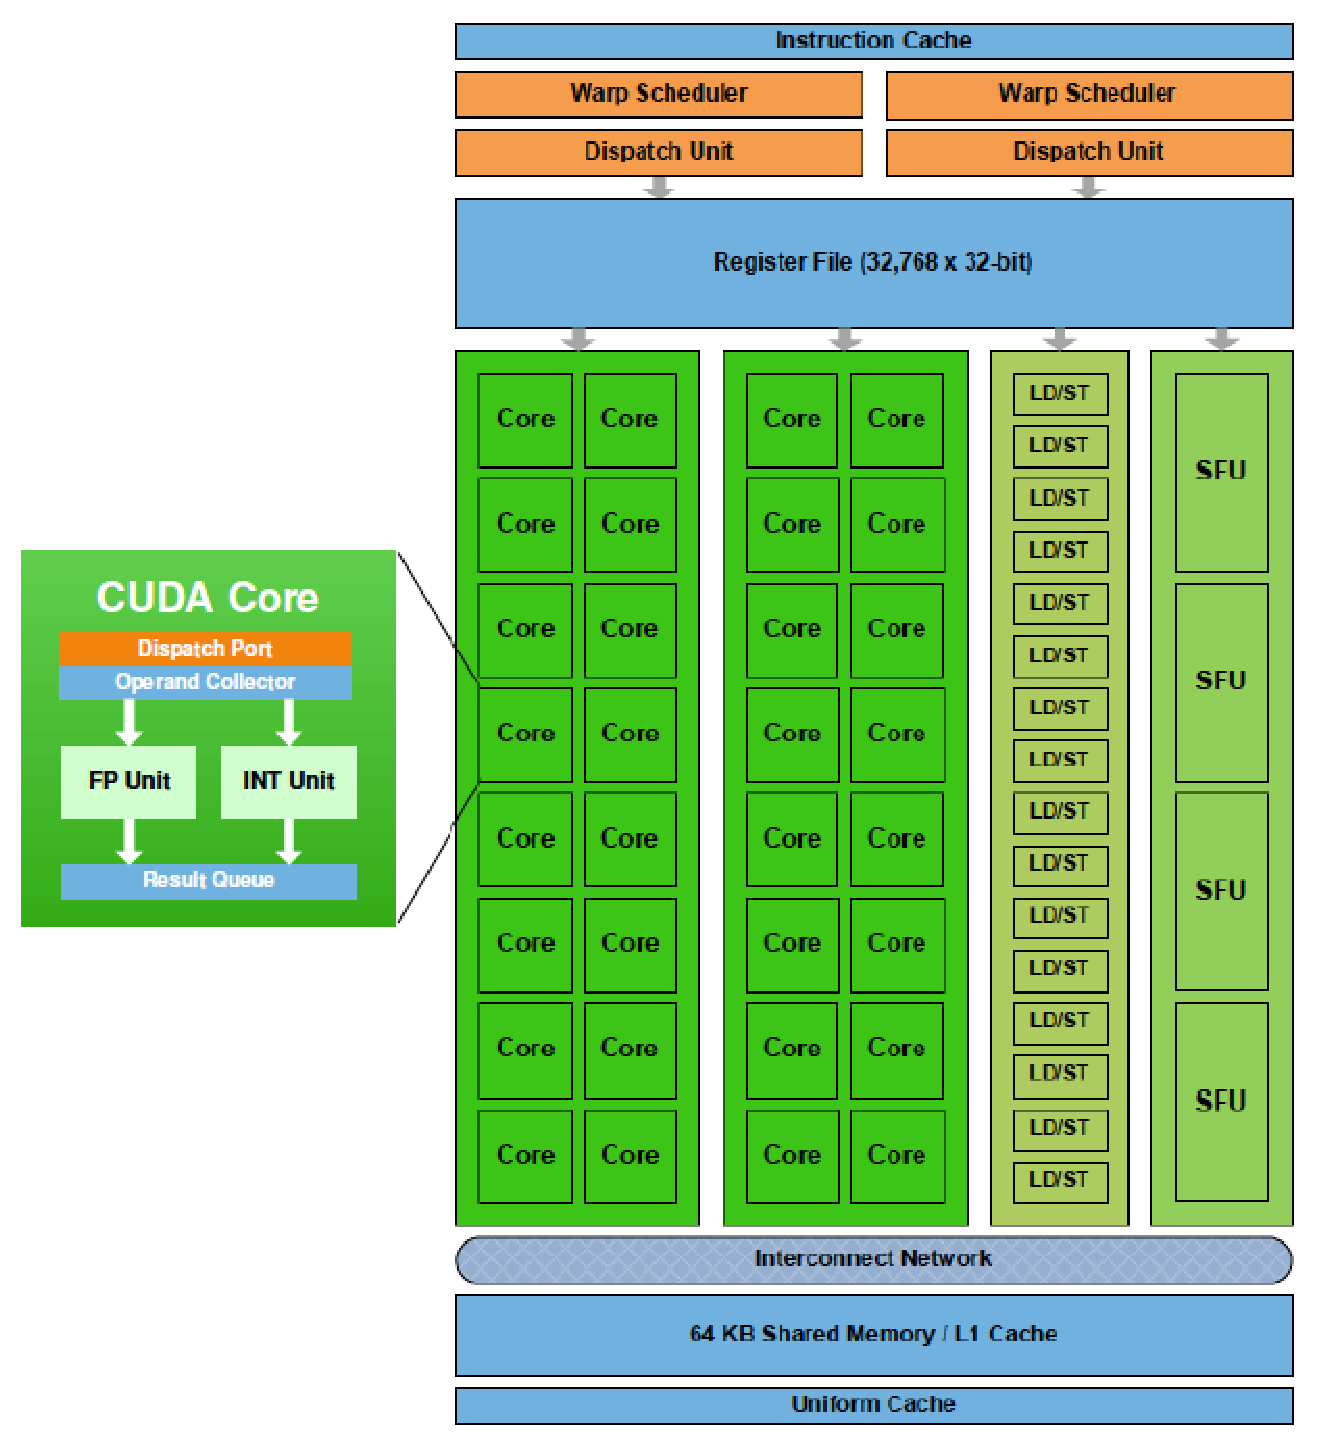
\includegraphics[height=10cm,
%     angle=0]{./images/gf100_sm.eps}}
% \caption{A streaming multiprocessor (SM) in Fermi (GF100)}
% \label{fig:gf100_sm}
% \end{figure}

There are many major changes in Fermi architecture, Fig.\ref{fig:gf100}. 
\begin{enumerate}
\item The GPU is orgnized into a number of GPC. The architecture of a single GPC
in GF100 is given in Fig.\ref{fig:Fermi_GPC}.

\item third generation SM in GF100 has 32 SPs and other stuffs, as shown in
Fig.\ref{fig:gf100}(B).

\item third generation SP use 40nm technology, now has a fully
  pipelined arithmetic logic unit (ALU) and floating point unit
  (FPU). It gives more SPs per chip (i.e. 512 SPs or 16 SMs or 4 GPCs)

  \begin{framed}
    Due to the limitation in 40nm architecture, Nvidia has to disable
    \begin{itemize}
    \item one SM, i.e. GTX 480 has 15 SMs with 480 CUDA cores
    \item two SMs, i.e. GTX 470 has 15 SMs with 448 CUDA
      core.
    \item a GPC, i.e.  result in a 384 core part with three raster
      engines and 12 PolyMorph engines.
    \end{itemize}
  \end{framed}



% , is
%  composed of one I-cache, 32 SPs + 4 TEX units + 16 load/store units + 4 SFUs +
%  2 warp schedulers with 1 dispatch unit
%   each + 1 Polymorph unit + 48KB+16KB L1 cache, registers, and other glue that
%   brought an SM together.

\item new (true) unified 768KB L2 cache are equally shared by all SMs
\item new shared/L1-cache memory configurable architecture (in 48/16KB
  or 16/48KB).
\item support higher accuracy with fused multiply-add (FMA)
  instruction
\item higher throughput in overall (memory, computational power,
  context switching...)
\item execute multiple task kernels at once

\item revise geometry units: PolyMorph units + Raster Engines
  \begin{itemize}
  \item 16 PolyMorph units (geometry units): each does 5 stages
    (Vertex Fetch, Tessellation, Viewpoint Transform, Attribute Setup
    and Stream Output) and serves a single SM. 
  \item 4 Raster Engines: each does 3 stages (Edge Setup, Rasterizer,
    Z-cull) and serves 4 SMs.
  \end{itemize}


  \begin{framed}
    Nvidia realizes that pure geometry performance increases only 3x
    from GFX5900 to GTX285, while pixel shading performance has
    increased by 150x. The reason is that geometry shading and
    tessellation requires a lot of works from the SM units in general,
    and data is frequently passed between SM and PolyMorph Engine, at
    different stages of rendering. So, Nvidia decided to bring
    PolyMorph unit closer to SMs, and add a separate hardware unit to
    do Tessellation - the Tessellator - to the PolyMorph
    engine. Nvidia expects to see a near 4x+ improvements in
    tessellation performance compared to AMD/ATI Radeon HD 5870.
  \end{framed}

  \begin{framed}
    Output of the PolyMorph engines are sent to the Raster Engines
    where it decides which pixels going to be viewed, and which should
    be discarded. After that, post-processing and pixel shading are
    done by the SMs.

  \end{framed}

\item 6 ROP partitions, each ROP partition has 8 ROP units, rather
  than 4. Totally, Fermi has 48 ROPs. 
  \begin{framed}
    For a while, the main bottleneck in graphical applications is the
    shader bound, i.e. not enough shaders. Now, with 512 cores in
    Fermi, it is no longer the issue, but the {\it pixel
      fillrate}.
    This is due to the rise of multi-screen gaming and Nvidia's 3D
    Vision. To increase the capabilities of pixel fillrate, Nvidia add
    more ROP units per partition.
  \end{framed}

\end{enumerate}

Another advances in software aspect is
\begin{enumerate}
\item C++ language support
\item better debugging support (Nvidia's Nexus plug-in in Microsoft
  Visual studio)
\item compatible with DirectX 11, OpenGL 3.x and OpenCL 1.x 
\end{enumerate}



\subsection{GF104/GF106/GF108}
\label{sec:GF104_GF106_GF108}

SUMMARY: GF104 has smaller memory bandwidth
      256 bits, with fewer CUDA core 384, less raster operators 32; yet more
      texture units 64. To achieve good performance with lesser resources; GF104
      need to run at a higher clock speed (overclocked).
      
The design of GF100 has many flaws inside that Nvidia has to revise it in
different models. One of the main reason to have GF104 is to reduce thermal and
power consumption. Other major changes, Fig.\ref{fig:GF104_100}:
\begin{enumerate}
  \item increase number of cores per SM, from 32 to 48
  \item increase dispatch port per core, from 1 to 2
  \item increase number of dispatch unit per SM, from 2 to 4. So, each warp
  scheduler has 2 dispatch units. 
  \item the number of SFU (special functional units) per SM, from 4 to 8, so it
  can process transcendental functions faster.
  \item texure units per SM, from 4 to 8 which has massive increase in graphical
  applications/games. 
  \item load/store units per SM, from 8 to 16
\end{enumerate}
Each GPC is kept the same with 4 SMs, along with a Polymorph Engines and a
common Raster Engine per
GPC\footnote{\url{http://www.hardwarecanucks.com/forum/hardware-canucks-reviews/34635-msi-geforce-gtx-460-cyclone-768mb-oc-review-2.html}}.
With 2 GPCs in GF104-based GPU, there are totally 2*4*48=384 SPs, 64 texture
units, 32 ROPs, 512KB of L2 cache and four 64-bit memory controllers.

\begin{figure}[hbt]
  \centerline{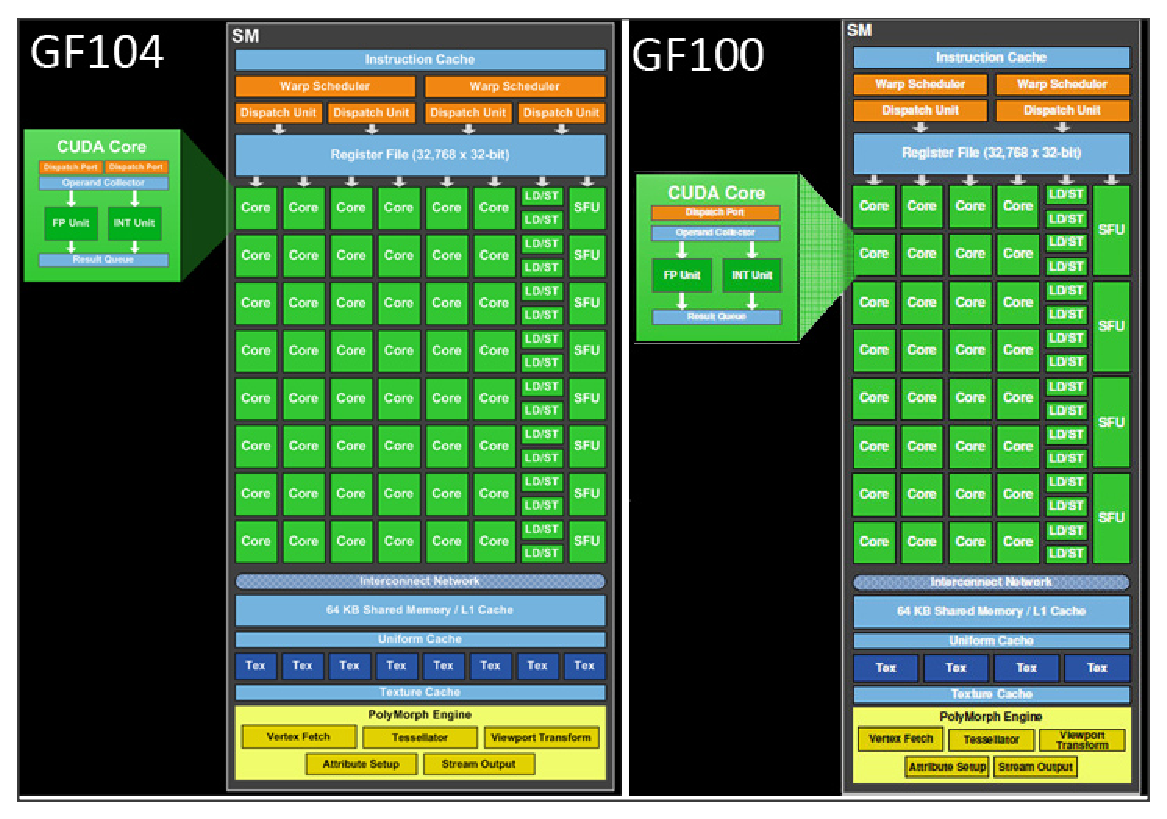
\includegraphics[height=8cm,
    angle=0]{./images/GF104_100.eps}}
\caption{GF104 vs. GF100}
\label{fig:GF104_100}
\end{figure}


\begin{framed}
GF100 use 529mm$^2$ die size. GF104 use 67mm$^2$ die size. The latter is
still 10\% larger than the closest rival, AMD Cypress/HD58xx with 334mm$^2$;
though both chips use the same 40nm
technology\footnote{\url{http://semiaccurate.com/2010/07/21/gf104gtx460-has-huge-die/}}.
GF108 use 130nm$^2$ die size, half of GF106.

GF104 has 1.95 billion transistor, GF100 has 3 billion. GF106 is lower-end and
GF108 is for integrated graphics. GF104 are gts 450,gts 440, gts 430. GF100
are Fermi card, GTX460, GTX48x. GF106 are GTX 445M.
\end{framed}

By increase the number of SPs per SM in GF104, the registers per core is
decreased compared to GF100. Besides, warp scheduler has double instruction
patch units (to 4, rather than 2). The reason for increasing from 32SPs per SM
to 48 SPs per SM (i.. 50\%), but double texture units, is that Nvidia think
tessellation engines is idling too much, so they want to decrease the number of Polymorph Engine per
CUDA core; and increase the shader processing per
PolyMorph\footnote{\url{http://www.pcper.com/reviews/Graphics-Cards/Nvidia-GeForce-GTX-460-Review-GF104-and-budget-Fermi}}.
GF106 has 4 PolyMorph engines (one per SM), and 32 texture units. GF108 tends to
be designed for entry-level cards. 

\subsection{GF110}
\label{sec:GF110}

GF110 is a significant revision from GF100. Fundamentally, GF110 use the same
architecture as GF100, with 32 SPs per SM. They use slower, lower-leakage
transistors in less time-sensitive path, and faster, higher-leakage transitors
in other areas. This allows using lower power and enable the 16th SMs, giving it
full 16 SMs working, i.e. totally 512 CUDA cores. GF110 has improved Z-cull
efficiency and can do FP16 texture filtering in 1 cycle, while GF100 needs 2
cycles\footnote{\url{http://www.tomshardware.com/reviews/geforce-gtx-580-gf110-geforce-gtx-480,2781-2.html}}.
In addition, GF110 use GF104 texture hardware, each unit can compute and fetch 4
32-bit/INT8 texture samples per clock, 4 64-bit/FP16 texture samples per clock
(GF100 can do only 2), and one 128-bit/FP32 texture sample per clock. This will
bring more performance on new games (which utilizes 64-bit texture samples).
\begin{itemize}
  \item  GeForce GTX 480 sported core/shader/memory frequencies of 700/1401/924
  MHz, 
  \item GeForce GTX 580 employs a 772 MHz core clock, a 1544 MHz shader
  frequency, and a 1002 MHz memory clock
\end{itemize}
{\it ``Excessive noise was one of the strongest reasons to avoid GeForce GTX
480, and it is effectively dealt with on the GTX 580.''}

In GF104, each SM can do 32 texels, compard to 96 instruction computed, giving
the ratio 1:3 (NOTE: shader clock is 2x the base (core) clock). In GF100 and
GF110, an SM can do 16 texels, or 64 instruction computed, giving the ratio 1:4 

\textcolor{red}{However, for computational purpose, GF100-based card like C2050
is still the first choice, with ECC memory, handling double-precision at half-rate of single
precision (whirl GF100 can handle double-precision one-quarter of the peak
performance)}.

\begin{framed}
 Z-culling is a method of improving GPU performance by throwing out pixels that
will never be seen early in the rendering process. By comparing the depth and
transparency of a new pixel to existing pixels in the Z-buffer, it's possible to
determine whether that pixel will be seen or not; pixels that fall behind other
opaque objects are discarded rather than rendered any further, saving on compute
and memory resources. GPUs have had this feature for ages, and after a spurt of
development early last decade under branded names such as HyperZ (AMD) and
Lightspeed Memory Architecture (Nvidia), Z-culling hasn't been promoted in great
detail since then. 
\end{framed}
\begin{enumerate}
  \item GF100: has 4
  GPCs\footnote{\url{http://www.tomshardware.com/reviews/geforce-gts-450-gf106-radeon-hd-5750,2734-2.html}}
  \begin{itemize}
    \item GTX 470 (1.25GB): 320-bit bus, bandwidth 133.9 GB/s
    \item GTX 480 (1.5GB): 384-bit bus, bandwidth 177.4 GB/s
  \end{itemize}
  \item GF104: has 2 GPCs, with total 336 shaders (SP or GPU core), with either
  192-bit bus or 256-bit bus
  \begin{itemize}
    \item GTX 460 768MB has 24 ROP units, 384 KB L2 cache, 192-bit bus,
    bandwidth 86.4 GB/s
    \item GTX 460 1GB has 32 ROP units, 512 KB L2 cache, 256-bit bus, bandwidth
    115.2 GB/s
  \end{itemize}
  Each  64-bit memory controller is attached to 8 ROP units.
  \item GF106 (a replacement for G92): has 1 GPCs, with total 1x4x48=192
  shaders, and a 192 bit bus
  \begin{itemize}
    \item GTS 450: 2 ROP units, 32 texture units, 128-bit bus, bandwidth 57.7
    GB/s.
  \end{itemize}
  \item GF108 has 128 shaders and a 128-bit bus. It use DDR3, rather than DDR5
  memory
  \item GF110:
  \begin{itemize}
    \item GTX 580 (1.5GB DDR5): with 512 cores, 64 texture units, 48 ROP units,
    384-bit bus, bandwidth 192.4 GB/s. 
  \end{itemize}
\end{enumerate}


\subsection{ROP}
\label{sec:rop}

{\bf ROP} does the last stage before output the pixel to the console
(screen or printer), e.g.  pixel blending, anti-aliasing, data
compression and other atomic memory operations. That's why the ROP
units interact directly with the global memory (i.e. framebuffer in
graphical term). The performance hasn't been changed (i.e. a single
ROP unit can process one 32-bit integer pixel per
\textcolor{red}{1 clock cycle}, one FP16 pixel over
\textcolor{red}{2 clock cycles}, and one FP32 pixel over
\textcolor{red}{4 clock cycles}); yet the atomic operations are
greatly optimized (i.e. 20x increase in the case of atomic operations
to a single thread, 7.5x for contiguous memory regions...).

\begin{framed}
  In Fermi, the framebuffer (aka the global memory) tie to each ROP
  partition is 64-bit memory bus $\rightarrow$ the chip has $6\times
  64=384$-bit GDDR5 memory bus. Even though it has a lower bit-wide
  than GT200, the rate per pin is double due to Fermi using GDDR5,
  rather than GDDR3. So in overall, it has better memory bandwidth.
\end{framed}

More ROPs capacity means better pixel fillrate (i.e. frame rates) with
higher levels of anti-aliasing, which is always a good
thing\footnote{\url{http://techreport.com/articles.x/14934/7}}.
\begin{itemize}
\item GeForce 7: has 4 ROP partitions, each with 4 ROP units. So
  totally, it has 16 ROP units.
\item G80: has 6 ROP partitions
\item G92: has 4 ROP partitions
\item GT200: has 8 ROP partition 

  In G80, G90, GT200, each ROP partition is composed of 4 ROP units
  and can output 4 pixels per clock.
  \textcolor{red}{ GT200 can draw pixels at a rate of 32 pixels per
    clock cycle}.

\item GF100: has 6 ROP partitions, yet a single ROP partition is
  composed of 8 raster execution units. All execution units share the
  L2 cache with the rest of GF100.

  Like previous generations, each ROP in Fermi can process 1 regular
  32bit pixel per clock, 1 FP16 pixel over 2 clocks, or 1 FP32 pixel
  over 4 clocks. Thus, with 48 ROP units,
  \textcolor{red}{GF100 can process 48 regular pixels per clock}. The
  ROPs are clocked together with the L2 cache.
\end{itemize}

\begin{figure}[hbt]
  \centerline{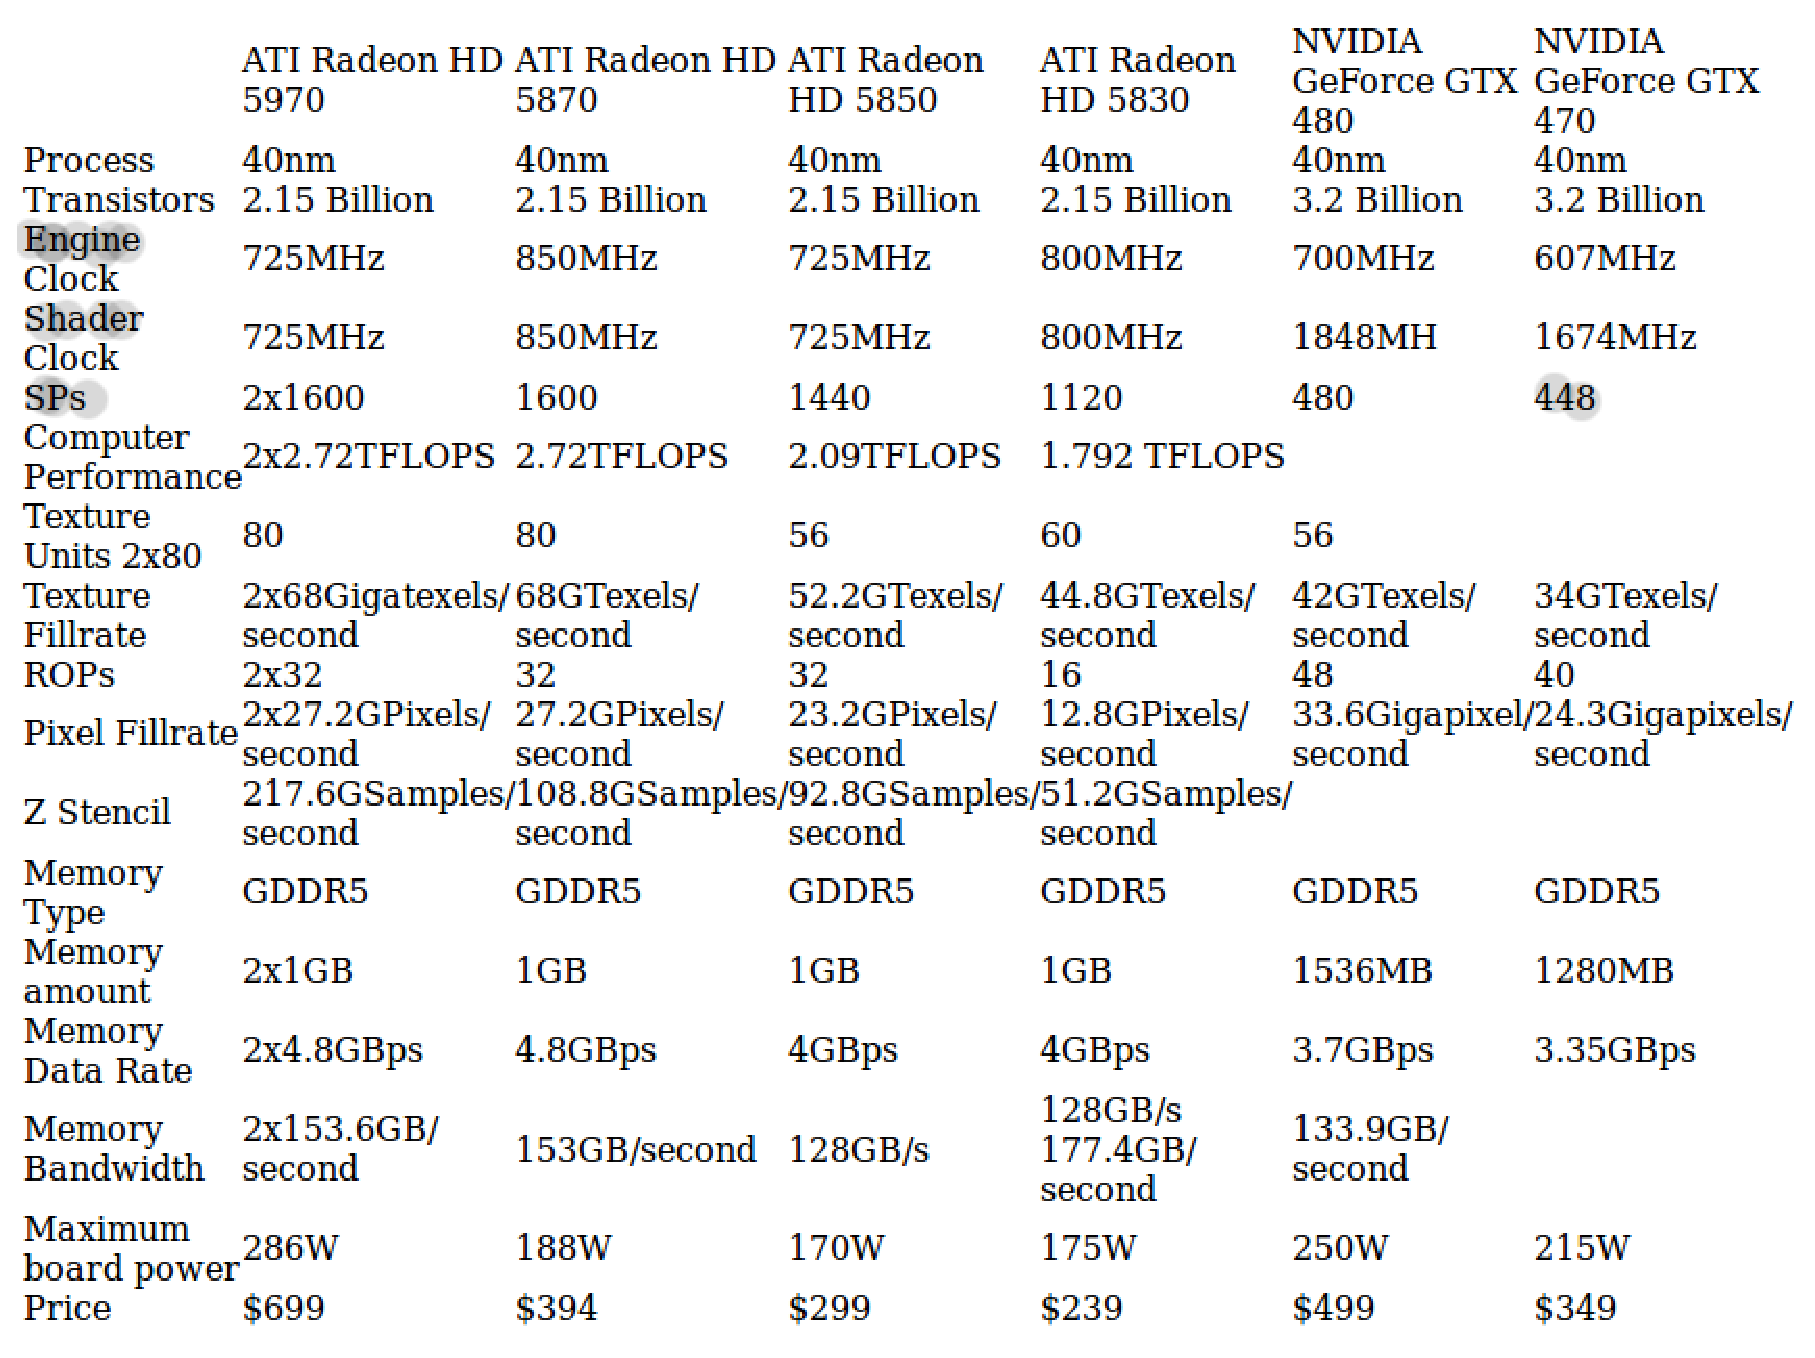
\includegraphics[height=10cm,
    angle=0]{./images/gpu_compare.eps}}
  \caption{GPU comparison}
  \label{fig:GPU_compare}
\end{figure}

The geometric details of the pixel are encoded into the 4
components. {\it Alpha testing} is a per-pixel technique being used to
determine whether to render a pixel to the screen or
not\footnote{\url{http://unity3d.com/support/documentation/Components/SL-AlphaTest.html}}
by comparing the alpha-value against a reference value. To achieve
better visual effect, instead of using render-or-not strategy, a
technique called {\it alpha blending} uses the alpha value to
determine how much the pixel contribute to the final image.  This can
produce soft edges, yet quite slow. {\it Alpha-to-coverage} basically
changes alpha blending into per-sample alpha testing. Another, better
technique is called {\bf transparency supersampling} (TSAA). A faster
but lower-quality anti-aliasing method than TSAA is Transparency
Multisampling (TMAA). The two methods are collectively called
{\it transparency anti-aliasing} and was introduced on the GeForce
7800GTX (G70) to fix issues with {\it alpha to coverage} on DirectX 9
games.

\begin{framed}
  The G70 was a DirectX 9 card and games running on these cards with
  TMAA on can look better. For the most part, TMAA is not a valid
  option as it doesn't really fix billboard aliasing. With the GF100
  and alpha to coverage, TMAA will have higher image quality in games
  that use it. The majority of games released today are still DirectX
  9 based, and TMAA will improve the image as it turns on alpha to
  coverage on DX 9 games.
\end{framed}

To avoid aliasing, (spatial) multi-sampling antialiasing (MSAA) [or
full scene anti-aliasing (FSAA)] technique is widely used in which the
picture is written out to the region of 2x or 4x the display
resolution, then down-sampled to match the display resolution. GeForce
8 support 8x MSAA. In addition, Nvidia also implement a new
anti-aliasing mode called {\it coverage sample anti-aliasing} (CSAA)
that improve the precision, yet only being used in special cases.
CSAA takes the color values of the FSAA such as 4x or 8x and applies
coverage samples to the pixel to smooth out lines without paying the
color sample cost of storage.

\begin{framed}
  More ROPs means the GPU can have better multisample anti-aliasing
  (MSAA) performance, Fig.~\ref{fig:anti_alias}.  The GF100 is expected
  to offer high performance with 8X MSAA, as the chip has more than
  three times the texture sample units of the GT200 and is geared to
  performance with 8X MSAA in mind. By way of comparison, the GeForce
  GT200 chip was architecture with 4x MSAA in mind, as it is limited in
  performance when 8x is enabled
  (8XQ)\footnote{\url{http://www.motherboards.org/reviews/hardware/2038_7.html}}.
\end{framed}

\begin{figure}[hbt]
  \centerline{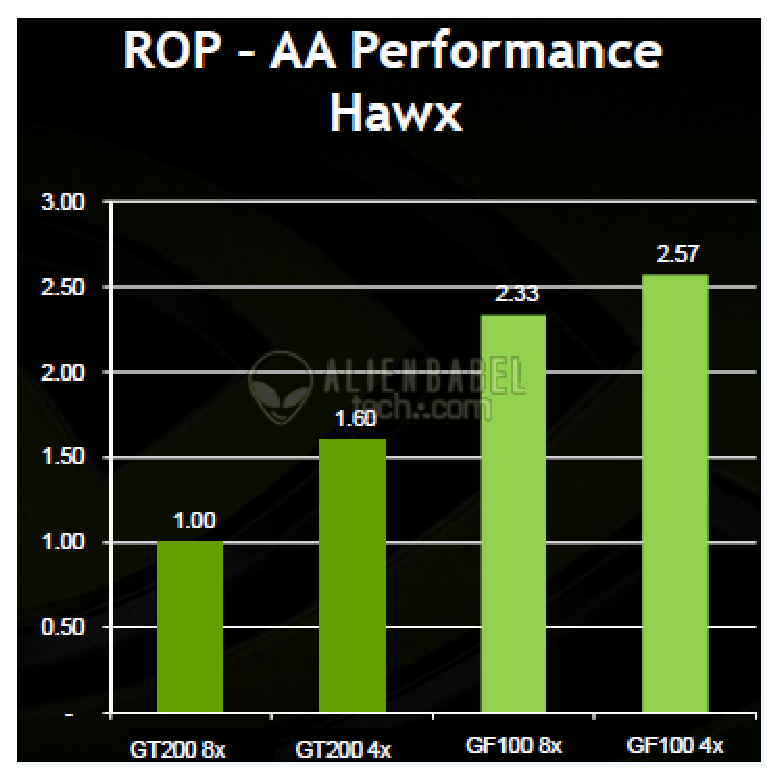
\includegraphics[height=5cm,
    angle=0]{./images/fermi_anti-alias.eps}}
  \caption{Anti-Aliasing (AA) performance comparison}
  \label{fig:anti_alias}
\end{figure}

Instead of using 8x MSAA, GF100 use 32X CSAA, and the possibility of
combining CSAA with MSAA to improve anti-aliasing of transparent
surfaces.. In 32x CSAA, the color values of 8x MSAA is stored with 24
additional coverage samples taken to a give better image quality than
8x by itself. The GF100 supports {\it alpha to coverage}
testing\footnote{\url{http://en.wikipedia.org/wiki/Alpha_to_coverage}}
which can allow the GF100 to blend fences, foliage and other fake
geometry that many games use.
\textcolor{red}{The GF100 can take up to 32 samples per pixel allowing
  up to 33 levels of transparency, compared to the 8 levels on the
  GT200}.


\subsection{Summary}
\label{sec:summary-CUDA_gpu_arch}


\begin{framed}
  The Texture Unit, ROP Unit, PolyMorph Engine and Raster Engine run
  at half the shader clock, rather than at the graphic core
  clock. GF100 is supposed to deliver 8x the geometry performance to
  GT200.
\end{framed}

The picture of GF100 (Fermi) is shown in Fig.~\ref{fig:gf100} (NOTE: 2
SMs are disabled). {\bf A GPC in Fermi has}
\begin{itemize}
\item 4 SMs
\item A Raster Engine. A Raster Engine processes 9 pixels per clock
  i.e.  \textcolor{red}{GF100 can process 32 pixels per clock}.
\item 4 Polymorph Engines
\end{itemize}

{\bf An SM in Fermi has}
\begin{itemize}
\item  32 SPs, instead of 8 SPs like GT200

\item  A Raster Engine. Each SM
  has\footnote{\url{http://www.geeks3d.com/20100118/Nvidia-gf100-architecture-details/}} 

\item 4 Texture units, i.e.
  \textcolor{red}{each GF100 chip has 56 texture units.}
\end{itemize}

\begin{framed}
  A GPC is basically a GPU without ROPs. There are totally 48 ROPs in
  Fermi. 
\end{framed}


References:
\begin{itemize}
\item \citep{lindholm2008ntu}
\item \url{http://www.motherboards.org/reviews/hardware/2038_6.html}
\item \url{http://www.behardware.com/articles/772-6/Nvidia-fermi-the-gpu-computing-revolution.html}
\item \url{http://alienbabeltech.com/abt//viewtopic.php?t=19846}
\item \url{http://www.pcper.com/article.php?aid=888}
\item \url{http://www.behardware.com/articles/644-4/Nvidia-geforce-8800-gtx-8800-gts.html}
\end{itemize}


\section{Tesla 4 (Kepler)}

Tesla 4 (Kepler) that use GK110 chip.




\section{When to use CUDA-capable GPU?}
\label{sec:when-use-cuda}

Recently, Intel has introduced Xeon Phi, a co-processor that use X86 ISA and
there is no need to change to existing codes. To program on CUDA-capable GPU, we
need to modify the codes so that in can run on PTX ISA. Before porting your
software to GPU or writing a new GPU-based software, you need to check the
following requirements for good performance on GPU

\begin{itemize}
\item the software must use a large number of threads

\item there should be a coherence in memory access by device code,
  i.e. data should be laid out to enable coalescing, data accessing
  among threads should have enough locality to use textures or (since
  Fermi) L1 efficiently, e.g. 128bytes cache line... 

\item data transfer between CPU vs. GPU must be minimized, i.e. data
  that are reused between kernels should be kept alive on GPU memory.
  \begin{itemize}
  \item Data on global memory are kept alive between kernels
  \item (since Fermi) Data on L2 cache are kept alive as well
  \end{itemize}

\item Ratio of operations (to be performed on GPU) to elements
  transferred (across CPU-GPU) should be high enough to achieve better
  performance. {\bf Example}:
  \begin{itemize}
  \item Matrices addition requires $3N^2$ elements to be transferred
    and $N^2$ operations (addition); thus the ratio is 1:3 or O(1)
  \item Matrices multiplication requires $3N^2$ elements to be
    transferred and $N^3$ operations (multiply-add); thus the ratio is
    1:N or O(N). 
  \end{itemize}
  As you can see, there is no benefit of using GPU for matrix
  addition; while we can get the benefit with matrices multiplication,
  especially when the matrices size getting larger.
\end{itemize}

\begin{framed}
  Code that cannot be sufficiently parallelized should run on the host,
  unless doing so would result in excessive data transfer between host
  vs. device. 
\end{framed}

The maximum speed-up of a serial program when running on $N$
processors is given by {\bf Amdahl's law}: If a fraction X of
computation is serialized, the speed up cannot be more than (1/(1-X)).
\begin{equation}
  \label{eq:2}
  S = \frac{1}{(1-P) + \frac{P}{N}}
\end{equation}
with $P$ is the fraction of the total serial execution time of the
code that can be parallelized over the total serial execution time of
the whole program. Suppose we have an unlimited number of processors,
then $P/N\approx 0$, or $S=1/(1-P)$. So, if $P=3/4$, we have maximum 4
times speed-up. It means that
\textcolor{red}{we need to spend more time on maximizing the amount of
  code that can be parallelized}.
\chapter{Fermi architecture}
\label{chap:fermi-architecture}

In the previous chapter, we have learnt important concepts of how a GPU work,
comparison between the architecture of a CPU vs. GPU, and a novel programming
model on Nvidia GPU, targetting to high-performance computing applications,
called CUDA. The main components of a CUDA-capable are streaming multiprocessors
(SMs, ranging several to tens) and global device memory.
Nvidia has developed the CUDA-enable GPU to a better design called Fermi
architecture, Fig.\ref{fig:summary_GPU}. We will discover in details in this
chapter. The design and architecture of a SMs can change from generation to
generation (e.g. Tesla 2 has 24 SPs per SM, GF100/GF100 has 32 SPs per SM, GF104
has 48 SPs per SM).

\begin{figure}[hbt]
  \centerline{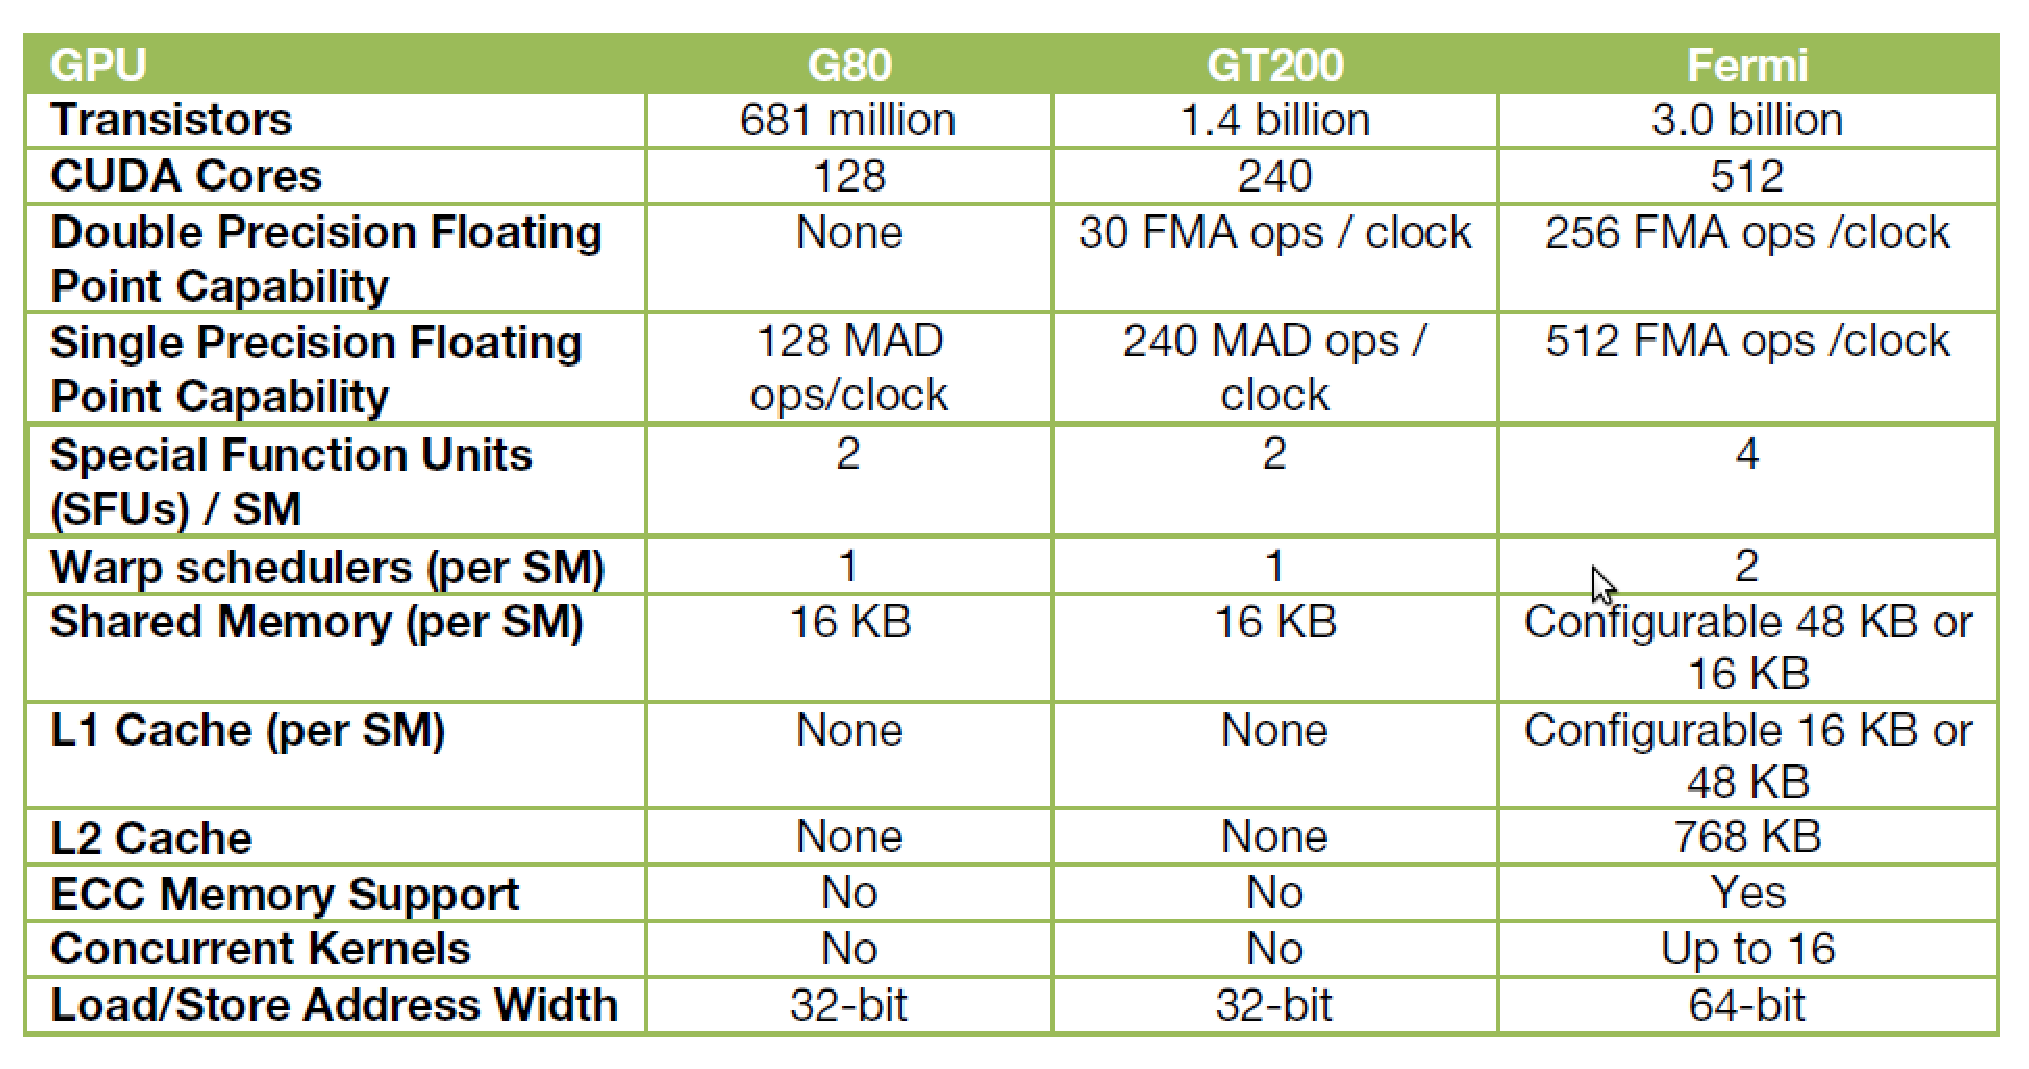
\includegraphics[height=5cm,
    angle=0]{./images/summary_GPU.eps}}
  \caption{Summary of CUDA-capable GPUs}
\label{fig:summary_GPU}
\end{figure}

Fermi is designed to improve performance upon Tesla (GT200) GPUs with special
emphasis on geometry, tessellation, and compute performance for DirectX 11.
\begin{enumerate}
  \item GeForce 256 (1999) has hardware transform and lightning.
  \item GeForce 3 (2001) has programmable shading
  \item GeForce FX has full 32-bit floating-point units
  \item GeForce 8 (2006) introduced unified, scalar shader design (CUDA)
  \item GeForce GTX 480 (GF100 = Fermi) ?????
  \item GeForce GTX 460 (Little Fermi)
  \item GeForce GTX 580 (Fermi Refined)
\end{enumerate}
 
\begin{figure}[hbt]
  \centerline{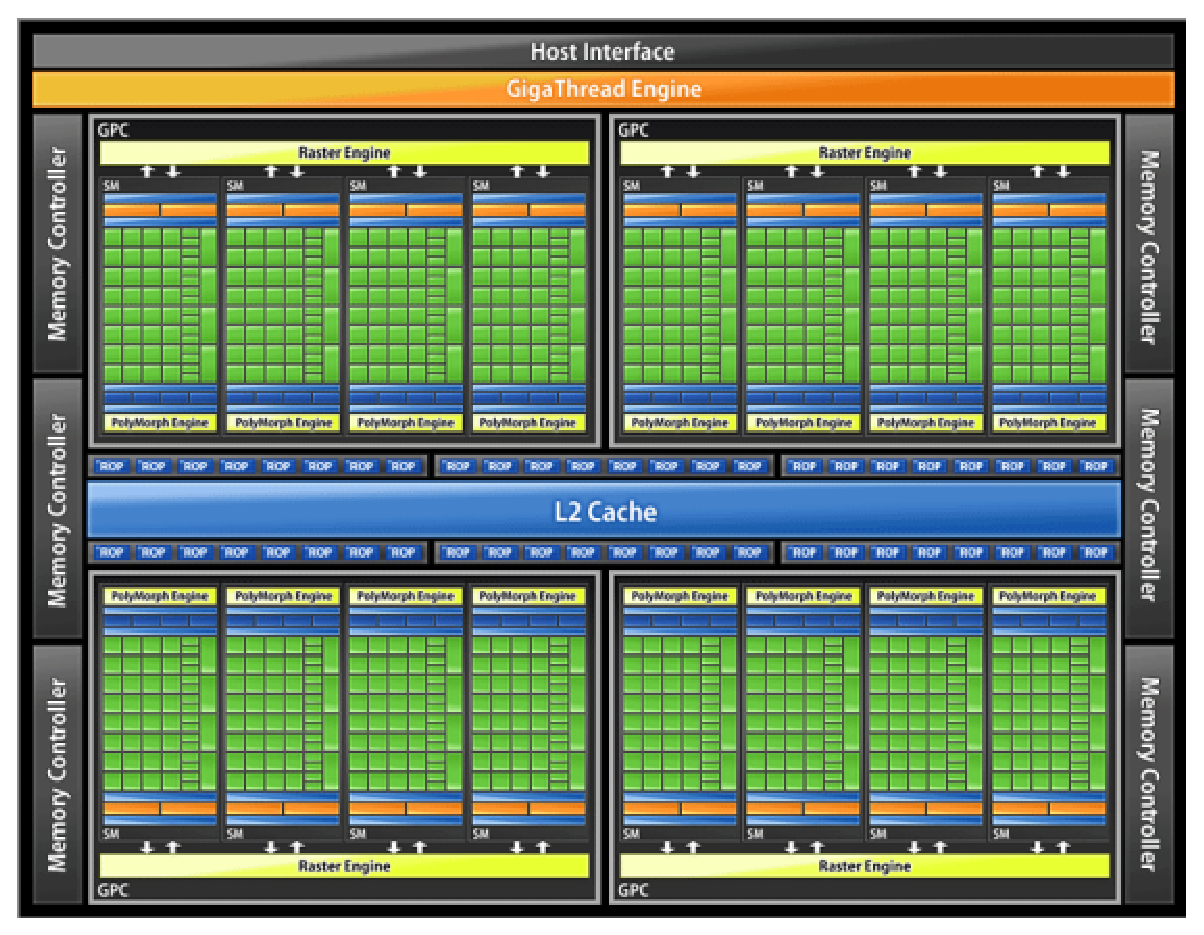
\includegraphics[height=8cm,
    angle=0]{./images/Fermi_C2070.eps}}
  \caption{Nvidia Fermi C2070}
  \label{fig:Fermi_C2070}
\end{figure}


CUDA integration allows full use of Visual Studio source-code
editors, inspectors, debuggers, profilers, and other productivity
features.  

Because Fermi fully supports exception handling at the hardware level,
programmers can set breakpoints in their CUDA source code and single-step
through a program while debugging using \verb!cuda-gdb!.  Visual Studio with
CUDA is currently in beta release.  To support debugging in prior GPUs, traps,
breakpoints or single-stepping first freeze the entire GPU state, and then the
CPU-based debugger reads and writes GPU thread registers, thread state, and GPU
memory over the link between system memory and GPU memory. The CPU based
debugger then resumes GPU execution.


In Fermi, two warps from different thread blocks (even different
kernels) can be issued and executed concurrently, increasing hardware
utilization and energy efficiency.

At any one time, the entire Fermi device is dedicated to a single
application. Fermi supports simultaneous execution of multiple kernels
from the same application, each kernel being distributed to one or
more SMs on the device.

Switching from one application to another is about 20 times faster on
Fermi (just 25 microseconds) than on previous-generation GPUs.


Like earlier GPUs, the Fermi architecture provides for local memory in
each SM.  New to Fermi is the ability to use some of this local memory
as a first-level (L1) cache for global memory references. The local
memory is 64K in size, and can be split 16K/48K or 48K/16K between L1
cache and shared memory.  The decision to allocate 16K or 48K of the
local memory as cache usually depends on two factors: how much shared
memory is needed, and how predictable the kernel's accesses to global
memory (usually the off-chip DRAM) are likely to be.
A larger shared-memory requirement argues for less cache; more frequent or
unpredictable accesses to larger regions of DRAM argues for more
cache.


Each Fermi GPU is also equipped with an L2 cache (768KB in size for a
512-core chip). The L2 cache covers GPU local DRAM as well as system
memory.


The final stage of the local memory hierarchy is the GPU's directly
connected DRAM. Fermi provides six 64-bit DRAM channels that support
SDDR3 and GDDR5 DRAMs. Up to 6GB of GDDR5 DRAM can be connected to the
chip for a significant boost in capacity and bandwidth over NVIDIA's
previous products.

Fermi is the first GPU to provide ECC (error correcting code)
protection for DRAM; the chip's register files, shared memories, L1
and L2 caches are also ECC protected. The level of protection is known
as SECDED: single (bit) error correction, double error
detection. SECDED is the usual level of protection in most ECCequipped
systems. Instead of each 64-bit memory channel carrying eight extra
bits for ECC information, NVIDIA has a proprietary (and undisclosed)
solution for packing the ECC bits into reserved lines of memory.

The total size of the registers (16 * 128 KB = 2048 KB) is larger than
the total size of the L1 caches (16 * 48 KB = 768 KB), and the total
size of the L1 caches equals the L2 cache size (768 KB)

Even though G80 had atomic instructions, the instructions operate on global
memory data. Since Fermi, by allowing these atomic values to be placed in the
shared L2 cache, atomic instructions can be 5X to 20X faster
(Sect.\ref{sec:atomic-functions}).


\section{Overview Fermi}
\label{sec:fermi_overview}

Fermi is designed based on 40nm technology, with 3.0 billion transistors. 

\subsection{Hardware specification of a Fermi GPU}
\label{sec:hardware-information}

In general, a Fermi-capable GPU has, as shown in Fig.\ref{fig:Fermi_C2070}.
\begin{enumerate}
  \item one Host Interface
  \item one GigaThread Engine
  \item 6 memory controllers, each is 64-bit GDDR5 1566 MHz
  \item 768 KB L2-cache shared by all CUDA cores
  \item CUDA cores are grouped into 4 GPC (Graphics Processing Clusters)
\end{enumerate}
Due to design challenge, there are different versions of Fermi-capable GPU, with
one or two SM disabled, e.g. GTX 470 and GTX 480, Fig.\ref{fig:gtx480_470}.
NVIDIA M2050 is a workstation level version of GTX 470 with 448
cores. C2050 is similar to M2050, except with a lower memory bandwidth
(144GB/sec compared to 148 GB/sec). The 1U server (2x M2050) or 4U
tower (4x C2050) enhance dramatically the performance.  

NOTE: A rack is typically 19-inch and 23-inch rack frames, which is about 42U high.

If $n$ is the number of rack units (i.e. $n$U), then the ideal panel height is 
\begin{equation}
h = (1.752n - 0.031)
\end{equation}
or the maximum rack units can be accomodated in a rack of $h$ U is
\begin{equation}
n_{\max} = (h + 0.031)/1.752
\end{equation}
So: $h = 42$, then $n \le 23.9$.

NOTE:
\begin{verbatim}
    Dimension (W x H x D)
1U    19" x 1.75" x 17.7"    (full-(width)-rack, but 1 unit height)
    19" x 1.75" x 19.7"
    19" x 1.75" x 21.5"
    
4U    19" x 7" x 17.8"    (half-rack, but 4 unit height)
    19" x 7" x 26.4"
\end{verbatim}



\begin{figure}[hbt]
  \centerline{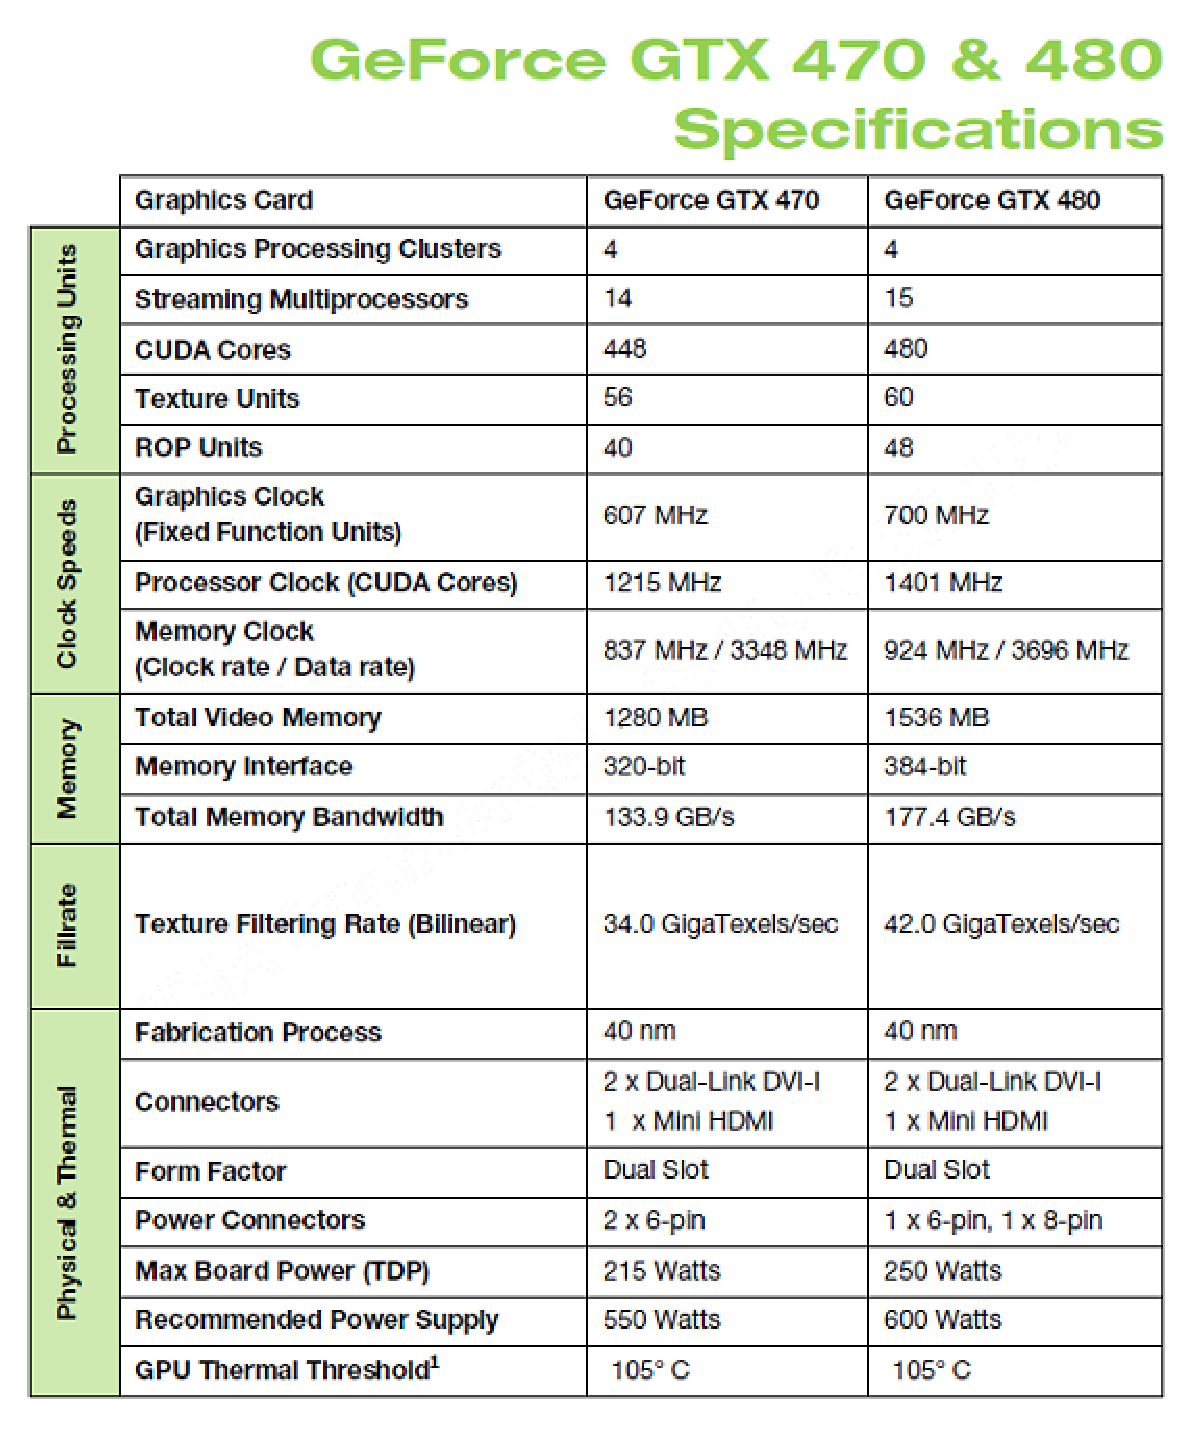
\includegraphics[height=9cm,
    angle=0]{./images/gtx480_470.eps}}
\caption{Comparison GTX 480 vs. GTX 470}
\label{fig:gtx480_470}
\end{figure}

\begin{enumerate}
\item Memory interface\footnote{\url{http://www.techspot.com/review/263-nvidia-geforce-gtx-480/page2.html}}
  \begin{itemize}
  \item Tesla 1st gen: 384-bit = six 64-bit wide memory controllers
  \item Tesla 2nd gen: 512-bit = eight 64-bit wide GDDR3 memory controllers (4GB
  DDR3)
  \item Fermi (GeForce GTX 470): 320-bit = five 64-bit memory
  controllers
  \item GeForce GTX 480: 384-bit = six 64-bit memory partitions $\rightarrow$
    support up to 6GB DDR5, e.g. 3GB DDR5 in C2050, 6GB in C2070. 
  \end{itemize}

\item GPU-CPU memory connection:
  \begin{itemize}
  \item G80: PCI-e Gen1 x16 
  \item G92, GT200: PCI-e Gen2 x16 
  \item GF100: PCI-e Gen2 x16 
  \end{itemize}

\item Clock rate: Different clocks rates are {\it core clock}, a {\it shader
clock} (fast clock)  and a {\it memory clock}. Memory clocks tell how fast the
memory run, i.e. the  memory bandwidth (depending on DDR3, DDR5...).  Depending
on the types of work (shading or general-purpose computing), a streaming
processor (SP) runs at either a higher clock rate ({\bf shader clock}) or a
lower clock rate ({\bf core clock}). In high performance computing, we only use
the concept {\it core clock}.
  \begin{itemize}
  \item G80 has shader clock as 1.35GHz; core clock at 575 MHz,
    memory clock at 999 MHz.
  \item G92 has shader clock as 1.8GHz; core clock at 738 MHz,
    memory clock at 1.1 GHz.
  \item GT200 has shader clock at 1.5GHz, core clock at 648 MHz,
    memory clock at 1.2 GHz.
  \item GT200x2 has shader clock at 1.25GHz, core clock at 576 MHz,
    memory clock at 999 MHz.
  \item Fermi has shader clock at 1.6GHz, core clock
    at 830 MHz (??? 1150 MHz), 
    memory clock at 3.6
    GHz (i.e. 1500 MHz)\footnote{\url{http://www.gigabyte.com/microsite/187/fermi-page.html}}. 
  \end{itemize}

\item Register files (per SM): shared equally by all {\it active} SPs
  in a SM (the concept of ``active'' to be discuss later)
  \begin{itemize}
  \item Tesla 1st gen:  8192 registers of 32-bit (total 32KB). Each
    SP can have 1K entries to be used by 96 threads.

  \item Tesla 2nd gen: 16384 registers of 32-bit (total 64KB,
    i.e. each SM has 16KB, i.e.
    \textcolor{red}{each SP has 2KB register files to be shared by up
      to 128 threads and probably supports 16 or 24 different banks}).
    \textcolor{blue}{Use a single double-precision data consume 2
      register files}.
    The register file is partitioned between thread blocks by the
    JIT/driver. Within the allocation for each thread block, register
    files are statistically assigned to a given thread at
    compile-time. So, we can explicitly tell the maximum number of
    registers to be used by a thread by using the compiler option
    \verb!maxregisters=n!.
    \textcolor{red}{In GT200, an individual thread can have minimum 4,
      maximum 128 registers}.

  \item Fermi: 32768 registers of 32-bit.
    \textcolor{blue}{In Fermi, a thread can have minimum 21 registers
      and maximum 63 registers per threads}

    NOTE:
    \textcolor{blue}{As an SM in Fermi has 4 times SPs compared to an
      SM in Tesla 2nd, the number of register files per thread is half
      compared to that in Tesla 2nd}.
    However, with the availability of L1/L2 cache and shared memory;
    it's hard to justify the performance difference just by looking at
    this.
  \end{itemize}

\item Shared memory:
  \begin{itemize}
  \item Tesla 1: 
  \item Tesla 2: each SM has 16KB shared memory (to be shared by all
    threads in a single block) divided into 16 equally banks. 
  \item Fermi: each SM has 64KB configurable shared memory divided
    into equally 32 banks
  \end{itemize}

\item Two read-only address space: constant vs. texture. 
  \begin{itemize}
  \item Tesla 1
  \item Tesla 2: 64KB constant
  \item Fermi: 
  \end{itemize}

% \item on-chip shared-memory vs. cache: read previous section


\item Special Function Unit (SFU): 
  \begin{itemize}
  \item GT200: each SM has 2 SFU 
  \item GF100: each SM has 4 SFU, i.e. double per SM compared to GT200
  \end{itemize}

\item Floating-point:

  \begin{itemize}
  \item Tesla 1st + 2nd gen: IEEE 754-1985 single-precision for MAD
    (multiply-add) with 128 MAD ops/clock
  \item Tesla 2nd gen: IEEE 754-1985 and increase to 240 MAD
    ops/clock; add support FMAD with 30 FMAD ops/clock,
    i.e. \textcolor{red}{1/8 slower than single-precision}
  \item Fermi: IEEE 754-2008, providing FMA for both single +
    double
    precision\footnote{give more accurate result for an expression}
    with 256 FMAD single-precision ops/clock and 512 FMAD
    double-precision ops/clock.
  \end{itemize}

\item Arithmetic operation for integer:
  \begin{itemize}
  \item Tesla 1st + 2nd gen: hardware support 24-bit; those require
    32-bit run in emulation mode
  \item Fermi: native hardware support 32-bit for all instructions,
    optimized to support 64-bit and extended precision operations
    also.
  \end{itemize}
\begin{figure}[hbt]
  \centerline{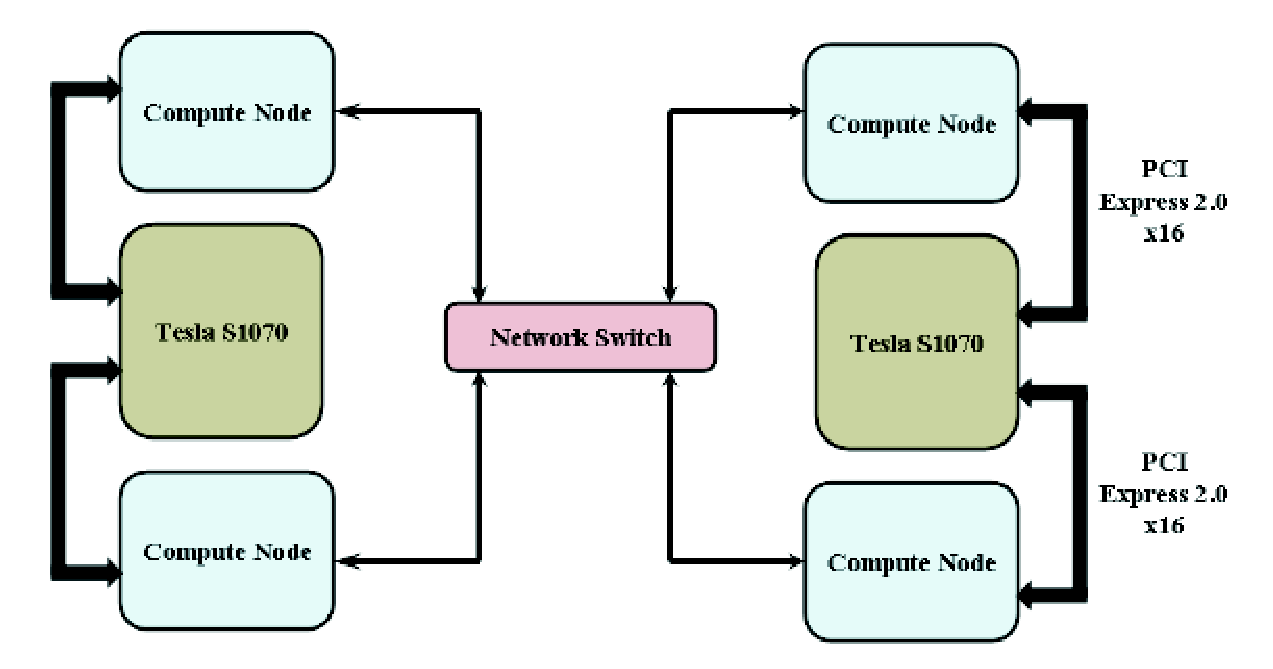
\includegraphics[height=5cm,
    angle=0]{./images/tesla_cluster.eps}}
\caption{GPU cluster: different machines connect via a network switch}
\label{fig:tesla_cluster}
\end{figure}

\item Load/Store (LD/ST) address width
  \begin{itemize}
  \item Tesla 1st + 2nd gen: one load/store unit of 32-bit. It means
    that only one kernel can use GPU at a time. So, if the kernel
    doesn't wide enough to span all cores; that hardware went idle,
    Fig.~\ref{fig:fermi_kernel}(a). 

  \item Fermi: 16 load/store units of 64-bit, i.e. 16 kernels can
    perform load/store data concurrently in a single clock, as shown
    in Fig.~\ref{fig:fermi_kernel}(B) (NOTE: only supports kernels
    from a single program. Kernels from two different programs need to
    run sequentially). However, you need to make sure the kernels are
    independent.  You will learn to create streams and assigning the
    kernel to appropriate stream ID.

  \end{itemize}
  \begin{figure}[hbt]
    \centerline{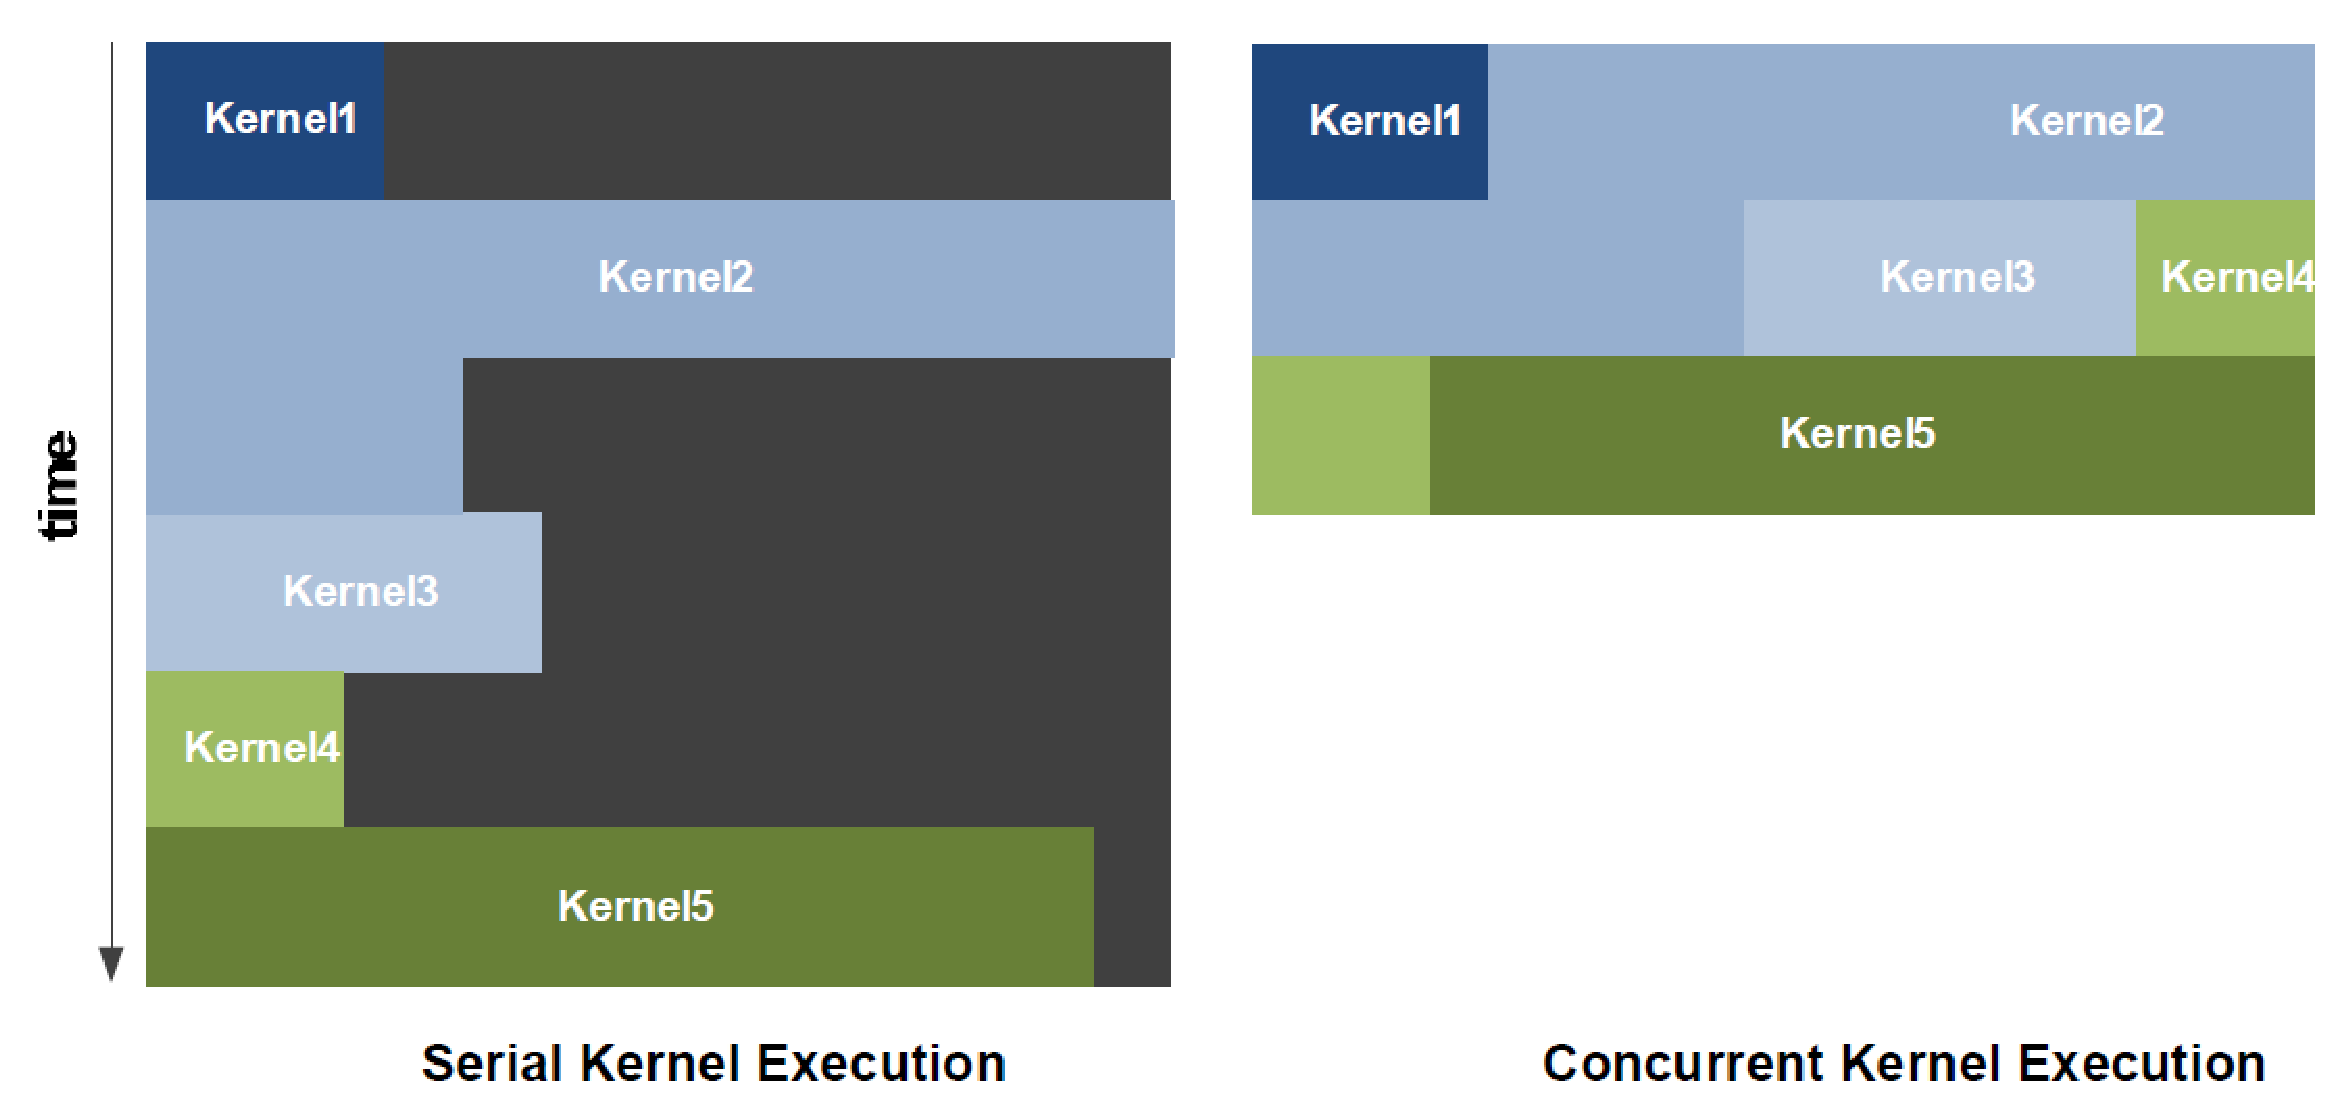
\includegraphics[height=5cm,
      angle=0]{./images/fermi_concurrent_kernel.eps}}
    \caption{(A) sequential kernel execution (B)Fermi concurrent kernels}
    \label{fig:fermi_kernel}
  \end{figure}

\item Context switching (each program receives a time slice of
  processor's resource)
  \begin{itemize}
  \item Tesla 1st + 2nd gen: 250 microseconds
  \item Fermi: below 25 microseconds (10x faster), concurrent
    kernel execution, better kernel-to-kernel communication
  \end{itemize}

\item Warp scheduler:
  \begin{itemize}
  \item Tesla 1st + 2nd gen: single warp scheduler $\rightarrow$ only
    a single kernel can run on GPU

  \item Fermi: two warp schedulers, with faster context switching,
    $\rightarrow$ allows more threads to be able to run in parallels,
    improved thread block scheduling.
  \end{itemize}

\end{enumerate}

 
\subsection{Fermi Streaming Multiprocessor (SM)}
\label{sec:fermi-sm}

Tesla GT200 has 8 CUDA core per SM. Each SM in Fermi, with 32 CUDA cores, can
handle 48 warps simultaneously. The CUDA core, again is a unified processor core
that can execute vertex, pixel, geometry, and compute kernels.

In Fermi, each streaming multiprocessors (SM) is composed of
\begin{enumerate}
\item a CU (control unit): decode/encode instructions, and schedule threads
\item a pipeline for execution: int, fp32, fp64, special-functions...
\item 32K of 32-bit registers (large, but potentially divided by
  thousands of threads; so number of registers per thread is
  limited). Each thread can have maximum 63 registers, and minimum 21
  (if threads fully populated).
\item shared memory (with register speed, but accessible to different
  threads) = a programmer-managed scratch-pad memory
\item L1 data cache, and constant cache: hardware-managed caches
\item texture unit : also hardware-managed cache, but is read-only and
  widely used for graphical application
\end{enumerate}

Each SM can allow maximum 1536 concurrent threads. 

Expectation:
\begin{enumerate}
 \item Fermi M2090: has 512 cores that can deliver 665 GFLOPs of peak
  double-processing performance. NOTE: Amber use four M2090 + one CPU can run
  69 nanosecond simulation in one day. The fastest performance on CPU for AMBER
  can deliver 46 ns/day. M2090 is equipped on server machine, not workstation
  \footnote{\url{http://pressroom.nvidia.com/easyir/customrel.do?easyirid=A0D622CE9F579F09&version=live&prid=757066&releasejsp=release_157&xhtml=true}}.
 
 \item Kepler C3070 can deliver 1.425 TFLOPs in double-precision, about 2.7
 times faster than C2050. 
 
 \item Maxwell C4070 can deliver 3.925 TFLOPs in double-precision, about 7.6
 times faster than Fermi C2070. 
\end{enumerate}

\begin{enumerate}
  \item 16 LD/ST units per SM: allowing source and destination address to be
  calculated for 16 threads per clock. Address can be in cache or global memory.
  
\item It supports up to 1536 concurrent threads
\item It has 32K 32-bit registers with \textcolor{red}{up to 63
    registers per thread} (21 if threads fully populated)

\item 4 SFU units: to execute transcendental functions (sin, cosine, reciprocal, and
square root). Each unit can execute one instruction per thread per clock. So a
warp of 32 threads take \textcolor{red}{8 clocks} to complete one transcendental
function.

\item Instruction throughput
  \begin{itemize}
  \item 2 fp32 pipes, each: 1 warp (or 32 threads) per 2 clock cycles
  \item 2 int32 pipes, each: 1 warp per 2 clock cycles
  \item 1 fp64: 1 warp per 4 clock cycles
  \item 1 SFU : 1 warp per 16 clock cycles (when using transcendental
    functions) 
  \end{itemize}

\item 64K total SMEM/L1 cache which can be partitioned into 16KB/48KB or
  48KB/16KB. The data in L1-cache can be shared between threads in the same SM
  (i.e. threads from the same grid block); but not across SM. Otherwise, we need
  to use L2-cache.

\begin{framed}

   We use more SMEM (48/16 configuration) to improve memory access for
   algorithms with well-defined memory access. Otherwise, L1 cache (16/48
   configuration) can be used to improve memory access for irregular algorithms
   where data addresses are not known beforehand.
   
   For graphics program, GF100 uses 48/16 configuration, where 16KB L1 cache
   acts as a buffer for register spills.
\end{framed} 

\item Shared memory (SMEM) is organized into 32 banks, each with
  32-bit wide. Now, support multicasting (previously only support
  broadcast). 

\item Coherent L2 cache with 128KB per memory controller, i.e. 768 KB
  in total. NOTE: AMD Cypress has 512 KB of L2. 

\item There is no native \verb!int64! instructions (integer
  arithmetic). However, there is magic to minimize needed \verb!int32!
  instructions. 
\end{enumerate}


\subsection{Graphic Enhancement}
\label{sec:Fermi_graphics-enhancement}

GF100 doubles the number of CUDA per SM (32 from 8). The geometry pipeline has
better geometry shading, stream out, and culling. GPC in GF100 features two
important innovations: (1) scalable Raster Engine for triangle setup,
rasterization, and Z-cull, and (2) a scalable PolyMorph Engine for vertex
attribute fetch and tessellation.

ROP units per ROP partition is doubled and fillrate is greatly improved. GF100
has 48 ROP units for pixel blending, antialiasing, and atomic memory operations.
The ROP units are organized in six groups of eight. Each group is serviced by a
64-bit memory controller

8xMSAA peformance is improved through enhanced ROP compression.

NOTE: The most advanced games use 1-2 milliions polygons per frame. In
computer-generated films, they use hundreds of millions of polygons. This is a
challenge to GPU, as the number of pixel shaders increased (from one to many
hundreds), but the triangle setup engine is still a singular unit. The two below
techniques are mostly used in films to create the intimately detailed
characters: tessellation + displacement mapping.
\begin{itemize}
  \item Tessellation: refines large triangles into a collection of small
  triangles
  \item Displacement mapping: change their relative position
\end{itemize}
GF100 can deliver high performance in tessellation and geometry throughput that
allows gaming applications to utilize the two techniques. Tessellation is
enhanced by the introducing of PolyMorph Engines (discussed below).

\begin{framed}
Objects and Characters in Games can be created using Software Modeling Packages:
MudBox, ZBrush, 3D Studio Max, Maya, SoftImage. The models are meshed of
triangles with associated texture maps need for proepr shading. In games, the
model information is sent per frame to the GPU through the Host Interface. 

Due to the limited bandwitdh of PCI-e bus, game developers tend to use
relatively simple geometric models. With the Tessellation unit on GPU, game
developers need to send a compact geometric representation of the
object/character, and the GPU can produce the correct geometric complexity for
the specific scene, Fig.\ref{fig:Ex_Tessellation}.
\end{framed}

\begin{figure}[hbt]
  \centerline{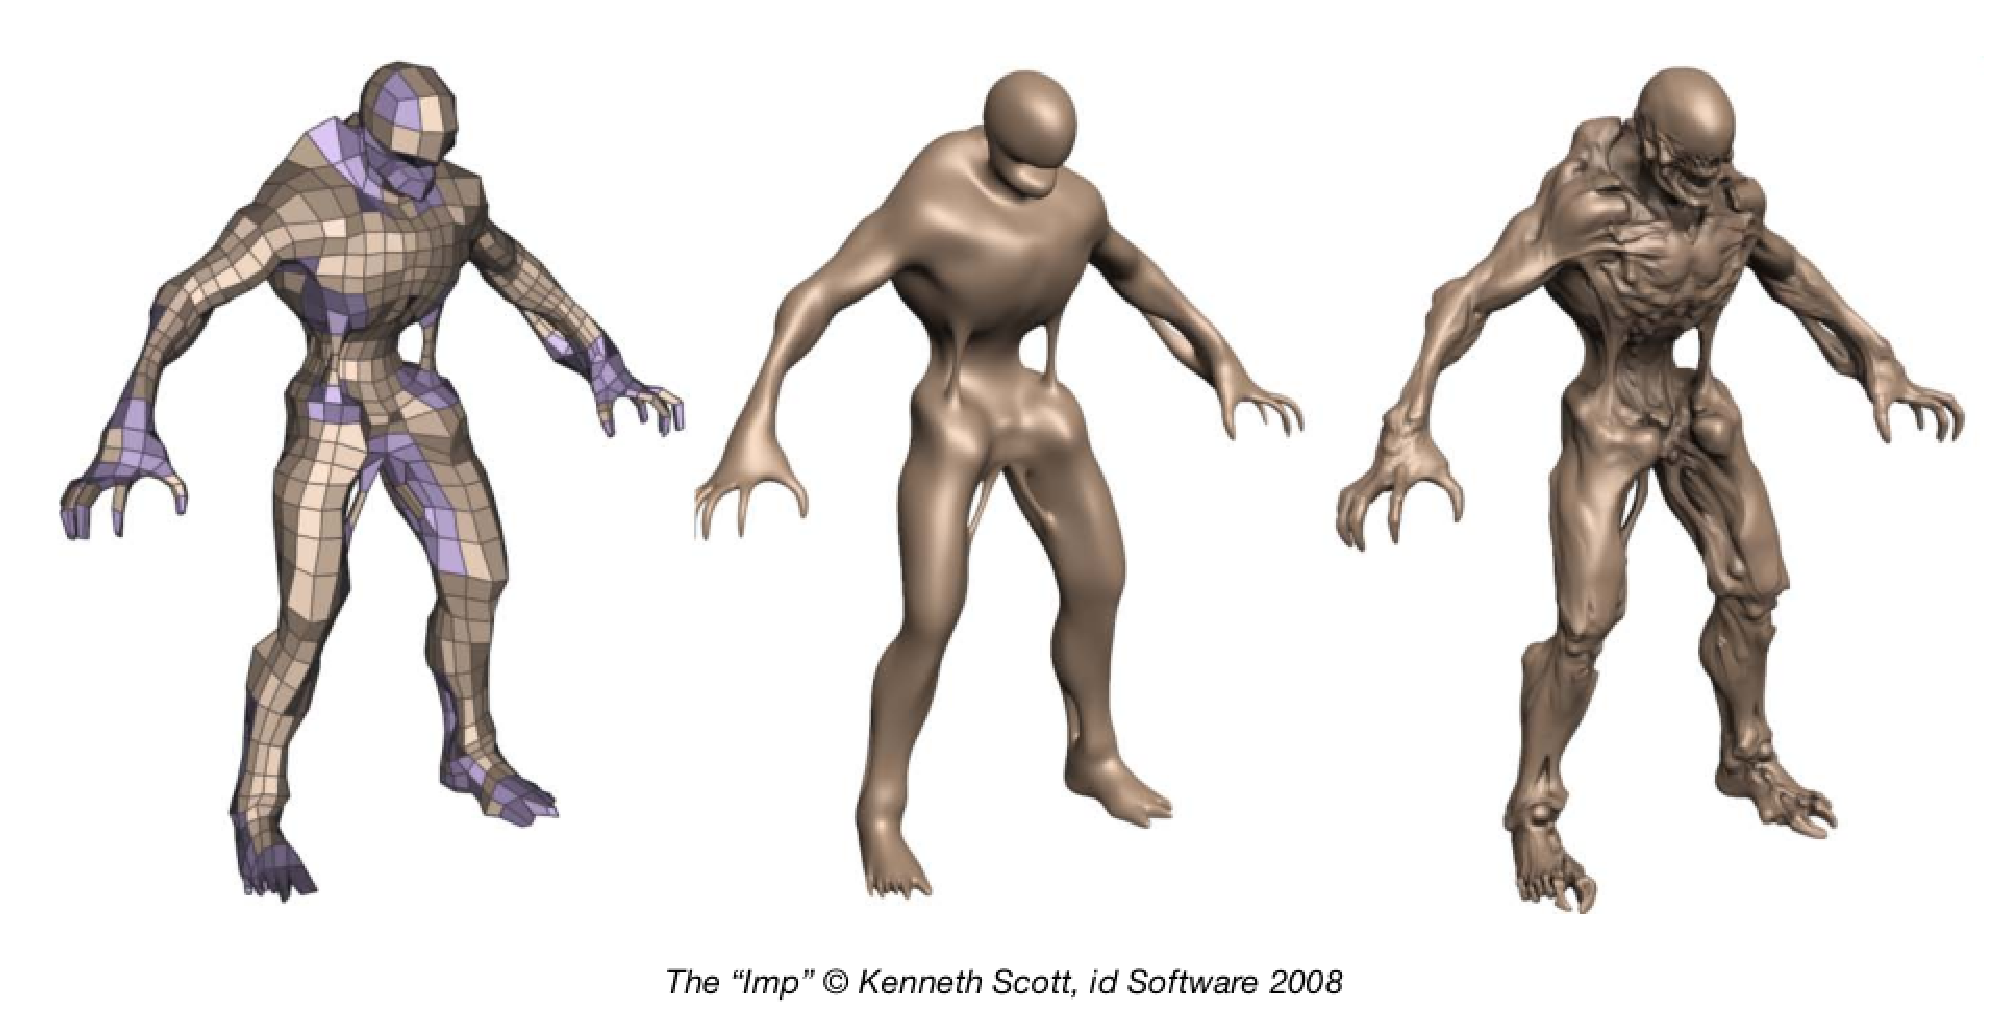
\includegraphics[height=5cm,
    angle=0]{./images/Ex_Tessellation.eps}}
  \caption{(A) A compact representation (quad mesh); (B) After Tessellation;
  (C) Tessellation first then applying Displacement Map}
  \label{fig:Ex_Tessellation}
\end{figure}


The traditional geometry processing architecture at the front-end of the
graphics pipeline is replaced by using multiple ``PolyMorph Engines''. Fermi
GF100 has 16 PolyMortph Engines. With tessellation, the triangle density
increases by multiple orders of magnitude. To rebalance the graphics pipeline to
handle high triangle rates, a scalable geometry called PolyMorph Engine is
developed (Sect.\ref{sec:polymorph-unit-+}).

On-chip L1 and L2 cache enables high bandwidth transfer of primitive attributes
between SM and the Tessellation Unit, and between different SMs. Tessellation
and all of its supporting stages can be done in parallel.

\subsection{Compute Enhancement}

GF100 has faster context-switching between graphics and PhysX (using GigaThread
Engine), concurrent kernel execution, and enhanced caching architecture (good
for irregular data access such as Ray Tracing).

GF100 has better atomic operations. GF100 implements IEEE 754-2008
floating-point standard, with FMA instruction for both single and double
precision. The newly designed integer ALU supports full 32-bit precision for all
instruction (i.e. native 32-bit integer arithmetic). Also, the integer ALU is
optimized to support 64-bit and extended precision operations. Double-precision
is now half-speed compared to single-precision.

New intrinsic operations: boolean, shift, move, compare, convert, bitfield
extract, bit-reverse insert and population count.

\section{Unified Virtual Address (UVA): from Fermi (CC 2.0) with CUDA 4.0}
\label{sec:UVA}
\label{sec:cuda4_UVA}


The NVIDIA Fermi GPU architecture, introduced in 2009, implemented a unified GPU
address space spanning the three main GPU memory spaces (thread private local
memory, thread block shared memory, and global memory) which was applied to
GPU-side data only (Sect.\ref{sec:SM-Fermi}).

In 2011, CUDA 4 introduced Unified Virtual Addressing (UVA) to provide a single
virtual memory address space for both CPU and GPU memory and enable pointers to
be accessed from GPU code no matter where in the system they reside, whether in
GPU memory (on the same or a different GPU), CPU memory, or on-chip shared
memory

The Fermi architecture support PTX ISA version 2.0, i.e. CC 2.0
(Sect.\ref{sec:CC2.0}).
PTX ISA 2.0 support unified virtual address space (UVA),
Fig.\ref{fig:Fermi-unified-address-space}, which is provided via CUDA 4.0 via 
the new API \verb!cudaHostAlloc! (Sect.\ref{sec:cudaHostAlloc}).

\begin{mdframed}

Previously, CUDA treats pointer to host-memory and pointer to device-memory differently.
Kernels can only uses pointers to device-memory (Sect.\ref{sec:GPU-pointer-pre-Fermi}).
Because of that, explicit calls to CUDA APIs to transfer data back and forth are required
\begin{verbatim}
cudaMemcpyHostToHost
cudaMemcpyHostToDevice
cudaMemcpyDeviceToHost
cudaMemcpyDeviceToDevice
\end{verbatim}
\end{mdframed}

UVA provides a single virtual memory address space, and the physical memory
where data resides is in fact on CPU side, i.e.  using the host memory from the
special memory region called th

In order to achieve UVA, the data is allocated on pinned CPU memory (pinned host
memory) or page-locked memory (Sect.\ref{sec:page-locked-memory}). This is
achieved by calling
\begin{verbatim}

\end{verbatim}

The pointer variable, pointing to data on page-locked memory, can be used on
GPU-side via PCI-e bus. This enables a single pointer, that is used for
accessing data from either GPU code or CPU code.

% , no matter where in the system they reside, whether its device memory (on the
% same or a different GPU), host memory, or on-chip shared memory.
\begin{itemize}

  \item The benefit is that data always reside on CPU-side. UVA does not
  automatically migrate data from one physical location to another, like Unified
  Memory does.

  Because of that, we say {\bf UVA enables “Zero-Copy” memory}, i.e. kernel code
  access the pinned host memory over PCI-Express, i.e. no 2 pointers mechanism
  is needed which always requires an explicit memcpy, and no implicit copy is
  done never.
  
Indeed, if zero-copy provided a degree of convenience in relation to data access
operations, UVA took this one step further by improving on data transfer tasks.

Zero-Copy provides some of the convenience of Unified Memory introduced in CUDA
6.0 (Sect.\ref{sec:Unified-Memory-CUDA6.0}), i.e. free users from managing the
explicit copy, but none of the performance, because it is always accessed with
PCI-Express’s low bandwidth and high latency.
  
\end{itemize}

The true benefit of the UVA mechanism becomes apparent when transferring data
between two devices. When all devices plus the host shared the same virtual
address space, a data access or data transfer involving two devices was
simplified in two respects:
\begin{enumerate}
  \item  Straight use on device A of a pointer to access memory on device B,

  \item  No need for staging the data transfer through host memory.
  
  Data can be transfered directly from GPU-1 memory to another GPU-2 memory,
  without having to copy first into the (intermediate) host memory.
  
  Here: data movement between GPUs through peer-to-peer transfers -
  Sect.\ref{sec:cudaMemcpyPeer}
  
\end{enumerate}
\url{https://www.nvidia.com/docs/IO/116711/sc11-multi-gpu.pdf}

CUDA 6.0 provides the TRUE unified memory - Sect.\ref{sec:Unified-Memory-CUDA6.0}.

Now, with unified memory and universal virtual addressing (UVA), one function
can handle all \verb!cudaMemcpyDefault!. As the virtual memory space used by UVA
is 40-bit memory space, the system need to be 64-bit. Data location becomes an
implementation detail, and it frees the programmer from handling this.

\begin{figure}[hbt]
  \centerline{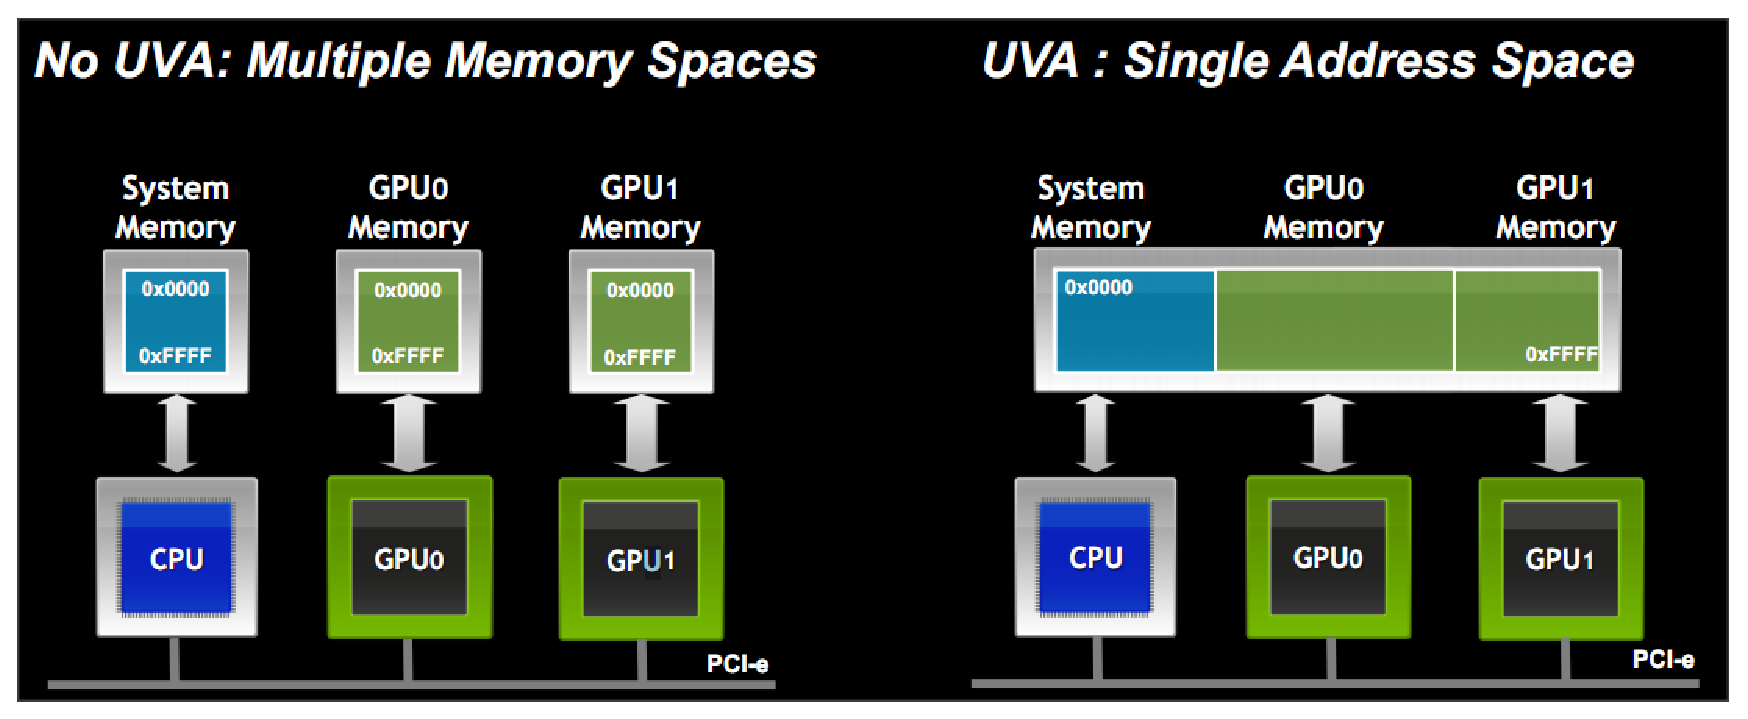
\includegraphics[height=5cm,
    angle=0]{./images/UVA_CUDA4.eps}}
\caption{UVA on Fermi-based GPU with CUDA 4.0}
\label{fig:fermi_UVA}
\end{figure}

In addition, same assembly instruction can be used for gmem,
smem... In addition, it enables function calling on GPU. % The space is
% 32-bit or 64-bit addresses with the default is based on the O.S. 
The space is still 40-bit, as with GT200. However, now local, shared
and global memory shared the same address space. So, you can use
pointers to point to data in any of those memories. 

\begin{figure}[hbt]
  \centerline{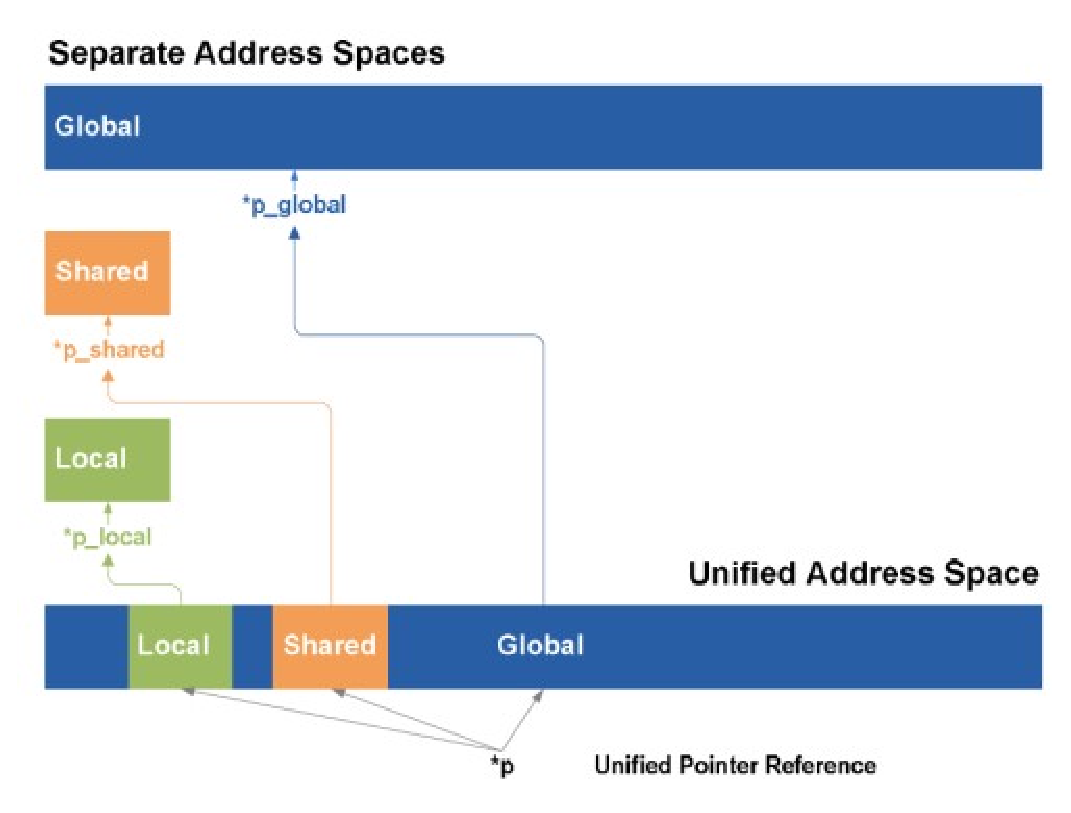
\includegraphics[height=5cm,
    angle=0]{./images/unified_memory.eps}}
\caption{Unified Memory pointers}
\label{fig:unified_memory}
\end{figure}

Using Direct Memory Access (DMA) on PCI-e Gen2, UVA allows
(Sect.\ref{sec:GPUs_share-data}:
\begin{enumerate}
  \item Direct Access
  \item Direct Transfer: Copy GPU A-GPU B without going through host memory
  (see requirements)
\end{enumerate}
Saturated bandwidth is $>$ 6GB/sec, and low latency: 1 PCI-e transaction + 1
memory fetch (about 2.5ns).

\textcolor{red}{CONS of UVA (compared to Unified Memory in CUDA 6.0+ and CC3.0+)}:
A device thread has to reach out to get the data. No guarantee of coherence is
provided as, for instance, the host could change the content of the pinned
memory while the device reads its content

   
\subsection{Physical and Virtual address space}
\label{sec:phys-virt-memory}

In early designs of Tesla architecture, it doesn't have virtual memory design,
only one kernel of a single program can use the GPU at a time. Now, Fermi
architecture supports CPU-style virtual memory architecture with 64-bit address
line, and physical memory with 40-bit address line (support up to 1TB of device
memory). This allows multiple kernels from a single program can run
simultaneously, i.e. each kernel use its own virtual address space, which then
can be mapped to the physical address by the GPU.

Even though kernel and host functions share the same virtual address space;
currently, kernel function cannot access host memory, and vice versa. So, all
data must be copied to GPU before passing it to the kernel; and all result must
be copied back to the host memory before passing it to a host subprogram.

\begin{figure}[hbt]
  \centerline{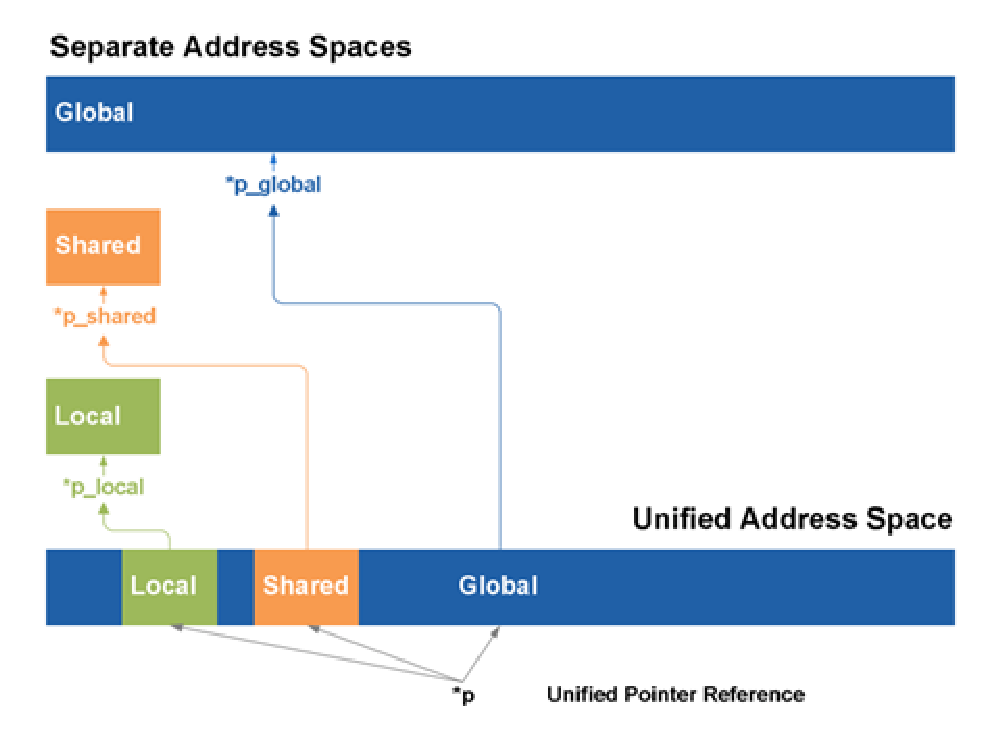
\includegraphics[height=6cm,
    angle=0]{./images/Fermi_unified-address-space.eps}}
  \caption{Fermi with CUDA 4.0+ using PTX 2.0 ISA share space with CPU}
  \label{fig:Fermi-unified-address-space}
\end{figure}


To check if the device supports unified addressing, we do
\begin{verbatim}
cudaPointerAttributes prop;
errorCode = cudaGetDeviceProperties  (prop, devID);

if (prop.unifiedAddressing == 1) then "Support"   
\end{verbatim}
NOTE: All devices with CC 2.0 and above running on 64-bit processes have unified
addressing enabled automatically. 

\begin{framed}
On Windows 7 and Vista, TCC driver model need to be used to enable unified
addressing. 
\end{framed}
 
\subsection{Data copy host $\leftrightarrow$ device, and device A
$\leftrightarrow$ device A}

Since this virtual memory share the same address space with CPU RAM, it's
impossible to tell if a pointer is pointing to a memory on CPU or GPU. This free
CUDA programmers from telling the CUDA driver APIs the direction of the data
transfer. So, to copy data from one location to another, we still use
\verb!cudaMemCpy()! yet we don't need to specify the direction.
Instead, we only use \verb!cudaMemcpyDefault! option.

\begin{verbatim}
errorCode = cudaMemcpy  ((void**) dst, (void**) src, numBytes,
        cudaMemcpyDefault);
        
cudaMemcpy(gpu0_buf, host_buf, buf_size, cudaMemcpyDefault)
cudaMemcpy(gpu1_buf, host_buf, buf_size, cudaMemcpyDefault)
cudaMemcpy(host_buf, gpu0_buf, buf_size, cudaMemcpyDefault)
cudaMemcpy(host_buf, gpu1_buf, buf_size, cudaMemcpyDefault)
\end{verbatim}

\begin{figure}[hbt]
  \centerline{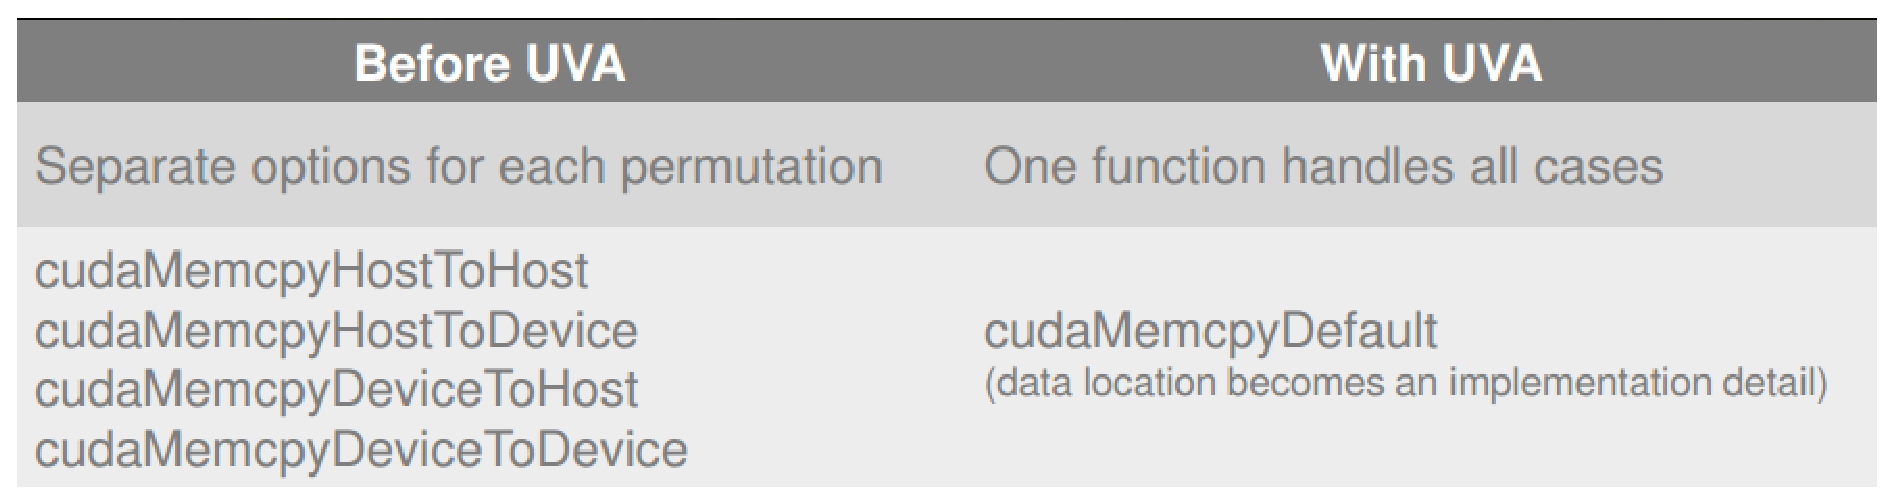
\includegraphics[height=3cm,
    angle=0]{./images/Fermi_UVA.eps}}
  \caption{UVA Fermi}
  \label{fig:Fermi_UVA}
\end{figure}

 
\subsection{Data copy device A $\leftrightarrow$ device B}

In 64-bit systems, if there is more than one devices on the system, they are
share the same virtual addressing space. As a result, CUDA 4.0+ support copy
data from one GPU to another GPU via DMA (direct memory access). This is known
as {\bf peer-to-peer memory copy}. This feature is used in GPUDirect technology
that allows using multiple-GPU (Sect.\ref{sec:multi-GPU_CUDA4.0}).

\begin{verbatim}
cudaMemcpy(gpu0_buf, gpu1_buf, buf_size, cudaMemcpyDefault) 
\end{verbatim}

Requirements:
\begin{enumerate}
  \item 2 GPUs on the same IOH
  \item Nvidia driver v270.41.19 or later
  \item CUDA 4.0+
  \item Fermi-class GPU
  \item 64-bit system
  \item Linux, or Windows with TCC driver.
\end{enumerate}

\section{Data and memory access}
\label{sec:data-memory-access}


\begin{enumerate}
\item Shared memory (SMEM) is programmer-managed scratch-pad memory

\item L1 data cache, constant cache: Hardware-managed caches

\item Texture unit: Hardware-managed cache for textures,
  interpolation/conversion unit
\end{enumerate}

\begin{figure}[hbt]
  \centerline{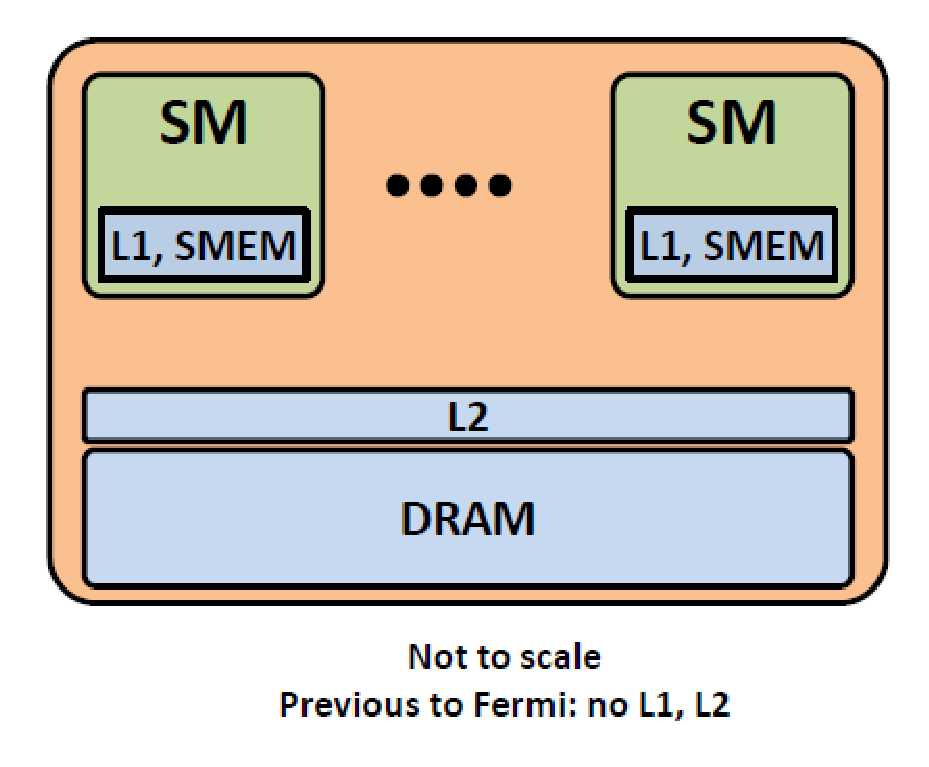
\includegraphics[height=5cm,
    angle=0]{./images/Fermi.eps}}
\caption{Fermi in brief}
\label{fig:Fermi}
\end{figure}

2D/3D thread blocks should be a multiple of 32 ``wide''. Data should
also be a multiple of 32 in the fastest-varying dimension. 


\section{Roles of constant memory and texture in Fermi???}
\label{sec:roles-const-text}

{\bf Questions: should we use texture cache or constant memory or L1
  and/or L2 cache?}

\begin{enumerate}
\item At first, and the most important, we only consider using texture
  cache or constant memory if the data is read-only.

\item Using constant memory is fast when the data is cached in the cache memory
and if all threads in the same half-warp read the same memory address
(Sect.\ref{sec:constant-memory}. Otherwise, sequential reads occur to these data
in the constant-cache memory.

\item Random load from texture could be a lot faster, than random load load from
  global memory. FERMI L1 cache to L2 datapath is 128 bytes wide, so
  with random access you could not use all L1 to L2(and memory)
  bandwidth. FERMI L1 texture cache to L2 datapath is 32 bytes wide
  (my guess!) , so random load is not a problem.

  i.e. Fermi L1 cache line size is 128 byte. If threads inside warp
  access different cache lines, EVEN if they all is inside L1 cache,
  your got 1/32 L1 theoretical bandwidth, because each thread issues
  one 128 byte transaction to get 4 byte float value.  Texture cache
  and shared memory don't have such problem.

\item Global memory accesses also could be 32 bytes wide, if they
  bypass L1 cache at all(compiler switch). With texture cache you get
  both: and L1, and small load granularity.
\end{enumerate}

\begin{framed}
  The cache line is the minimum amount of data that a single thread
  retrieve from memory (e.g. 128 bytes), regardless of how many data
  it truly needs (e.g. 32 or 64 bytes). So, 
  \begin{itemize}
  \item if threads read 4-byte data in the same cache lines, we only
    need a single memory read
  \item if threads read 4-byte data, each element in a separate cache
    lines (though all data elements are residing in the L1 cache), we
    still need individual memory read for a single thread, which means
    we only use 1/32 theoretical bandwidth; and that slow down the
    performance 
  \end{itemize}

  As texture cache has the cache line is 32-bytes, then if a single
  thread read in float4 data, i.e. 8-byte, the penalty is 1/4; rather
  than 1/32. 
\end{framed}

I think using texture still have many benefits in accessing data
located in CUDAArray (optimize for 2D and 3D).

its probably dependant on the access pattern.  I saw 20-30\%
degragation going from textures to gmem (i.e. textures were faster),
even with L1, with the following access pattern.
\begin{lstlisting}
float fValue = tex1DFetch( tex1, iIndex ) * w1 + 
     tex1DFetch( tex1, iIndex + 1 );  //or get a float2 out of the
                      //textures.... 

\end{lstlisting}
For me L1 seems just to make things worse (increasing L1 to 48K and
reducing Shared mem to 16K also reduced occupancy and resulted in
slower performance) - I guess it was mostly usefull for register
spilling enabling me to use the -maxrregcount and thus increase
occupancy by moving spilled registers to the L1.


I asked Michael Garland about textures vs. L1 in his presentation for
at the VSCSE summer school last week. He confirmed what we are saying
here, that sometimes L1 is better and sometimes the tex cache was
better for the sparse matrix vector multiply kernels he works on. The
interesting thing he added is this:
\textcolor{red}{added benefits are possible by making use of both
  caches in a single kernel}.
They are independent caches, after all!
\textcolor{red}{The idea is to read from one array with tex1Dfetch (or
  tex2D/3D) and from the others with L1}.
1) It limits the L1 cache pollution and 2) It gives you a larger
amount of cache memory to read from.

I've only got one kernel that performs cached reads from 2 different
arrays which I can try this idea out on - it did lead to a slight
performance improvement. The improvement likely wasn't that great
because the 2nd array read is not in the inner loop and only performed
once for every ~30-40 inner loop random reads.

It is too bad that the tex cache is so shrouded in secrecy that we
can't know what access patterns work well for it. Even a cache line
size would be something! 

Many people experience a drop in performance when trying to use 64KB
L1
cache\footnote{\url{http://forums.nvidia.com/index.php?showtopic=167561}}.
It's better to use L2 cache only (i.e. use \verb!-dlcm=cg! compiler
option). 

Shared memory doesn't have cache lines at all.

There's a big difference between cache lines and banks. Cache lines
are groups of 128 contiguous bytes aligned to 128 byte
boundaries. GF100 copies values from device memory to L2 and from L2
to L1 in these 128 byte chunks.

Banks are unrelated to cache lines. GF100 shared/L1 has 32 banks, each
corresponding to the low order words of the address. At each
instruction tick, each bank can output its 4-byte-word to one thread
who requests a word with that low order address. If two threads
request different memory with the same low order word addresses, the
bank can only service one of them, and another instruction tick is
needed to service the next.. they're serialized. (There's an exception
for a single word broadcast of the identical address though.)

Your quote from the programming manual discusses a different topic,
multi-word accesses by threads. L1 behaves just like shared memory in
this case, with identical inevitable bank conflicts.

\begin{framed}
  I think it's clear now that threads of the same warp in my program
  are accessing different cache lines of L1 cache that make it worse
  than texture cache. L1 cache is accessed in the unit of 128-bit
  cache lines. And what about texture cache? How was it accessed?
\end{framed}

In GT200, constant memory access is recommended to use known offset
(for ...) and threadIdx.x as offset (for ...). In Fermi, constant
memory access with known offset is essentially free.  In addition,
Fermi is RISC processor, with instruction arguments come from
registers, immediate constants or constant buffer. Otherwise, separate
load instruction is needed

There are two cases of constant memory
\begin{enumerate}
\item the constant data is literal, i.e. part of the instruction
  itself, e.g. 3.1415
\begin{lstlisting}
mul.f32 r0 r1 3.1415
\end{lstlisting}

\item the constant data need to be loaded from constant memory
\begin{lstlisting}
mul.f32 r0 r1 c0[10]
\end{lstlisting}
  The data from c0[10] is loaded into the register r1. However, we
  don't need a separate memory load instruction

\end{enumerate}

Example: to add value from constant memory you need only one
instruction
\begin{lstlisting}
add.f32 r0 r0 c2[0x35]
\end{lstlisting}

Example: to add value from global memory you need a load and an add
\begin{lstlisting}
ld.u32 r1 g[0x35]
add r0 r0 r1
\end{lstlisting}

\begin{lstlisting}
#immediate constant
set $p0 ne u32 $r4 -0x1

#constant buffer
add b32 $r12 shl $r13 0x2 c2[0xc8]

#global memory
ld b32 $r4 ca g[$r12(null)+0]

#constant buffer with unknown offset
ld b32 $r17 c2[$r17(null)+0x20]
\end{lstlisting}

Constant memory:
\begin{enumerate}
\item a bit faster than from global memory
\item doesn't require separate load instruction
\end{enumerate}

Texture load is faster than normal global memory. Global memory load
granularity is 128 bytes. It means that if you only need 4 bytes, the
hardware also fetches 124 neighboring bytes too. Texture load
granularity is 128 bytes at L1 level and 32 bytes at L2 level. So,
depending on compiling setting, you can determine which one to use. 

Fermi L1 cache line size is 128 byte. If threads inside warp access
different cache lines, EVEN if they all is inside L1 cache, your got
1/32 L1 theoretical bandwidth, because each thread issues one 128 byte
transaction to get 4 byte float value.  Texture cache cache line is
32-byte so float can be accessed alone by individual threads.  Thus
texture cache and shared memory don't have such problem.

A cache line in L1 or L2 is 128 bytes and maps to a 128-byte aligned
segment in device memory.  If the size of the words accessed by each
thread is more than 4 bytes, a memory request by a warp is first split
into separate 128-byte memory requests that are issued independently.
Each memory request is then broken down into cache line requests that
are issued independently. A cache line request is serviced at the
throughput of L1 or L2 cache in case of a cache hit, or at the
throughput of device memory, otherwise.


Texture:
\begin{enumerate}
\item random load from texture is a lot faster than load from global
  memory 

\item Fermi 12KB L1 texture cache (per 4 texture units) and L2 datapath is
32-byte wide, so random is not a problem. A random access means non-regular and is
  defined as (1) random or unknown at runtime, or (2) access pattern
  is non-linear (neither is it square or cubic)
\begin{lstlisting}
int offset = random()%SIZE;
int value = array[offset];
\end{lstlisting}
  The speedup of texture memory (besides free interpolation from 2D/3D
  to 1D) is when you access it linearly or in a blockwise fashion
  (2-d). if you're storing to shared memory you can definitely read it
  in linearly. maybe in each block read in (x-2,y-2) to (x+w+2,y+h+2)
  and then run the filter in parallel from (x,y) to (x+w,y+h).

  an advantage of this is that varying your filter size will have a
  fairly neglible effect on your i/o utilization. and it's deliberate
  and exact instead of cacheing which is more heuristic and might make
  the wrong decisions.


\item As Fermi L1 and L2 cache is to 128-byte wide, with random
  access, we doesn't utilize all L1 and L2 memory bandwidth. In other
  words, texture is a better choice for non-sequential or random
  memory access, especially in 2D and/or 3D data structure.

\item Global memory access could also be 32-byte wide, if they bypass
  L cache at all (need to use compiler switch). 
\end{enumerate}

NOTE: If we have a filter of 5x5 array. It means we need to use this
array by all threads. Then you can (1) use constant memory, or (2) we
can use shared memory and achieve about 25x speed-up. 


NOTE: Accessing 5x5 subarray, e.g. in matrix multiplication, is not a
random memory access. Each pixel is read $5\times 5 = 25$ times.
Indeed, it follow the patterns and the $i$-th thread reads
\verb!a[i+const]!  element


Shared is universally much faster than L1 cache hit reads in GF100. In
GF 104, they're about the same if there's access of the same cache
line at once but L1 is slower if different cache lines are read
simultaneously.


as i understand it on 2.0 or greater you can split it 16kb and 48kb or
vice-versa.

but the point is that you have a regular access pattern so with shared
memory you can use that knowledge of the access pattern to make sure
that there is never a "cache miss".  whereas if you use cache, it's
going to be dependant on scheduler decisions which can be pretty
random so it might swap out memory when you're not done with it
resulting in a big performance loss.

and that's the general rule: caches are great for random access, but
when you know the access pattern ahead of time and it's regular, well
you can use that knowledge to your advantage (e.g. reducing "misses")
by statically-scheduling memory fetches, e.g. via shared memory.

though if this is the only kernel that'll be running on the gpu at
that time, it's arguable how random the scheduling will be. doesn't
hurt to try both ways out.

On devices of compute capability 1.x, some kernels can achieve a
speedup when using (cached) texture fetches rather than regular global
memory loads (e.g., when the regular loads do not coalesce
well). Unless texture fetches provide other benefits such as address
calculations or texture filtering (Section 5.3.2.5), this optimization
can be counter-productive on devices of compute capability 2.0,
however, since global memory loads are cached in L1 and the L1 cache
has higher bandwidth than the texture cache.


But for my program, I still got speedup by using texture memory on GTX
480 even if I configure the L1 cache to be 48KB. I'm confused about it
because I don't use other benefits provided by texture memory and L1
cache is much large than the texture cache also. I want to know why?
One possible reason is that texture cache is used exclusively but L1
cache is shared by all the memory accesses. Is that reasonable?

References:
\begin{itemize}
\item \url{http://forums.nvidia.com/index.php?showtopic=176567}
\item \url{http://forums.nvidia.com/index.php?showtopic=181432}
\item \url{http://forums.nvidia.com/index.php?showtopic=186514}
\item
  \url{http://www.geforce.com/#/Hardware/GPUs/geforce-gtx-580/architecture} 
\end{itemize}
\section{Kernel in parallel}
\label{sec:kernel-parallel}

Now, Fermi supports up to 16 kernels (not perhaps not as quite as many
in practice) at the same time, giving that there is no dependence
between them. 

Parallel kernels can share SM. However, this requires two kernels to use the
same cache/shared memory configuration. 

\section{Kernel configuration}
\label{sec:kernel-configuration}

Fermi hardware does support 3D grids (which is why they are in the PTX
spec) but they're not exposed in the current CUDA API. This should be
in the next release.

\section{New capabilities}
\label{sec:new-capabilities}

\begin{itemize}
\item ECC for DRAM, L1, L2, shared memory. To turn it off, type
either the commands below, then reboot the  machine.
\begin{verbatim}
nvidia-smi -e 0

nvidia-smi -g 0 --ecc-config=0

-r    --gpu-reset           Trigger secondary bus reset of the GPU.
                            Can be used to reset GPU HW state in situations
                            that would otherwise require a machine reboot.
                            Typically useful if a double bit ECC error has
                            occurred.
                            --id= switch is mandatory for this switch
\end{verbatim}
NOTE: ECC can only handle single-bit errors, if there are double-bit ECC errors,
then the card should be replaced.

To check for ECC error, run \verb!nvidia-smi -q! on Linux
\begin{verbatim}
    Ecc Mode
        Current                     : Enabled
        Pending                     : Enabled
    ECC Errors
        Volatile
            Single Bit            
                Device Memory       : 0
                Register File       : 0
                L1 Cache            : 0
                L2 Cache            : 0
                Texture Memory      : N/A
                Total               : 0
            Double Bit            
                Device Memory       : 0
                Register File       : 0
                L1 Cache            : 0
                L2 Cache            : 0
                Texture Memory      : N/A
                Total               : 0
        Aggregate
            Single Bit            
                Device Memory       : N/A
                Register File       : N/A
                L1 Cache            : N/A
                L2 Cache            : N/A
                Texture Memory      : N/A
                Total               : 0
            Double Bit            
                Device Memory       : N/A
                Register File       : N/A
                L1 Cache            : N/A
                L2 Cache            : N/A
                Texture Memory      : N/A
                Total               : 309590
    Retired Pages
        Single Bit ECC              : N/A
        Double Bit ECC              : N/A
        Pending                     : N/A
    Temperature
        Gpu                         : 51 C

    Clocks
        Graphics                    : 50 MHz
        SM                          : 101 MHz
        Memory                      : 135 MHz
    Max Clocks
        Graphics                    : 573 MHz
        SM                          : 1147 MHz
        Memory                      : 1500 MHz

\end{verbatim}


\item Fermi has 2 copy-engines, thus GPU-CPU and CPU-GPU can be done
  concurrently. Previous generations can do one direction at a time
\item Fermi can execute multiple kernels at the same time. At first,
  the GPU must have free resource. Second, the kernels must be on
  different streams. Thirdly, the two kernels must NOT be dependent on
  data. 
\end{itemize}

\begin{figure}[hbt]
  \centerline{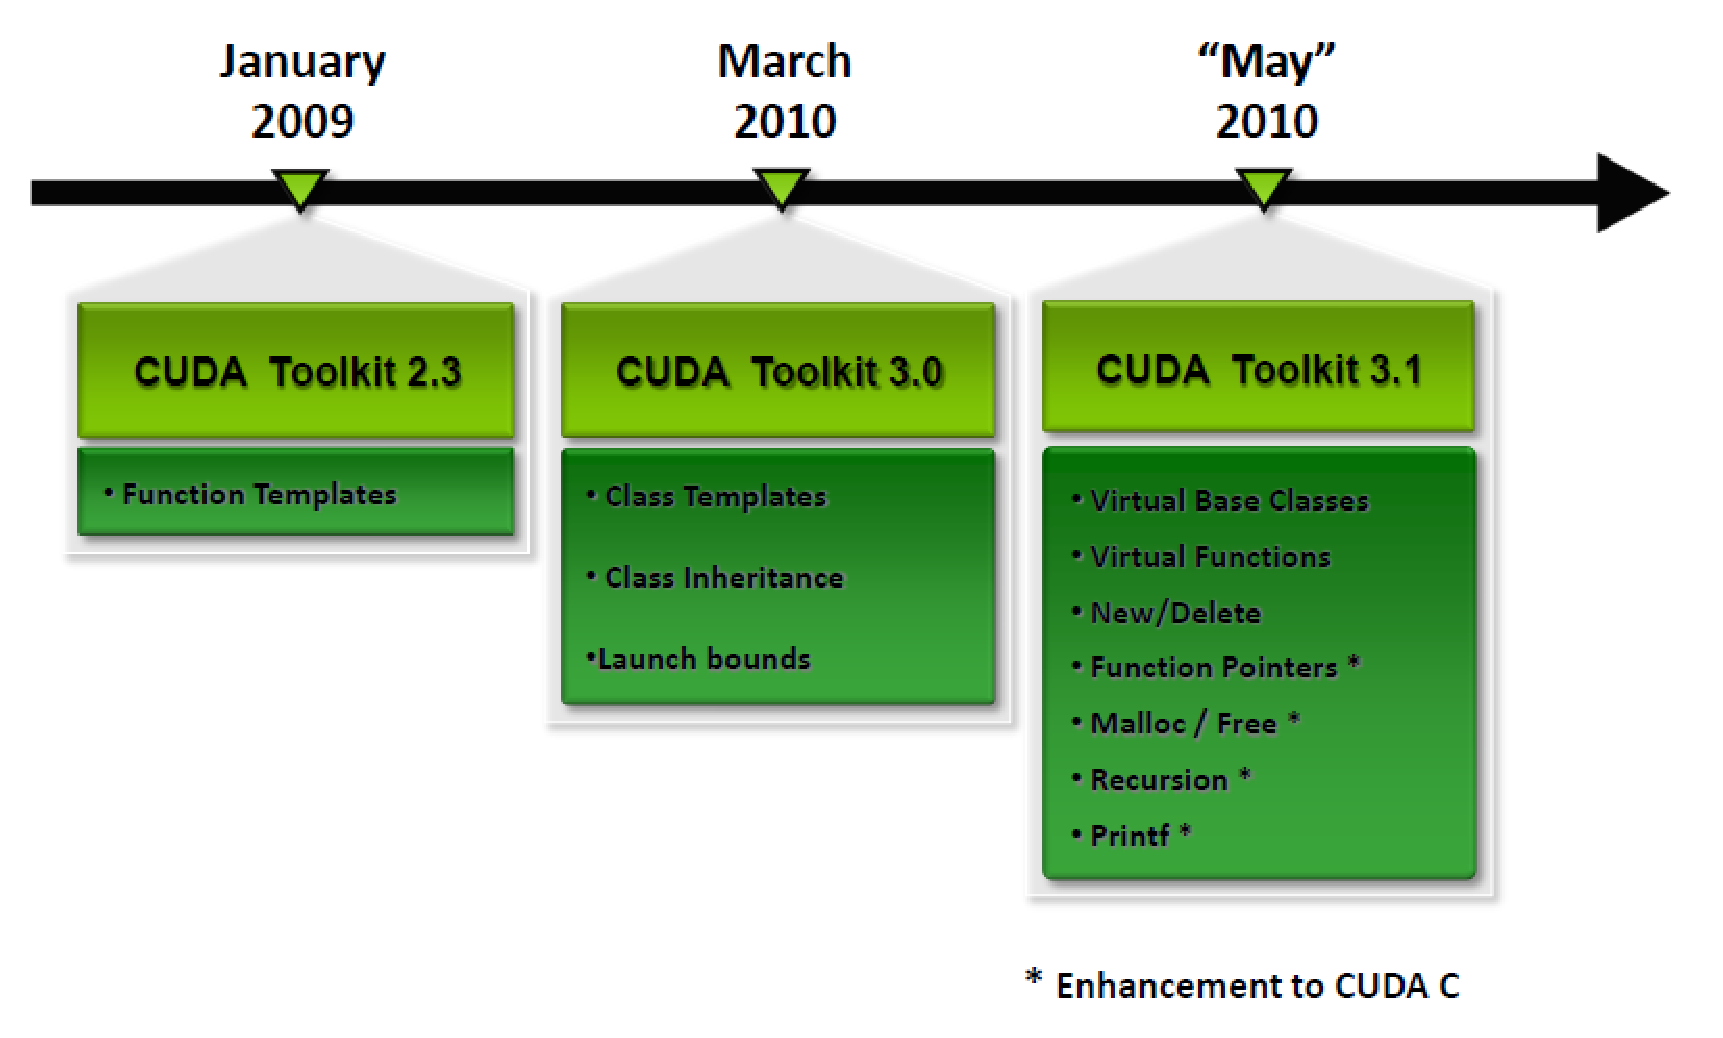
\includegraphics[height=5cm,
    angle=0]{./images/CUDA_C_new.eps}}
\caption{CUDA C improvements}
\label{fig:CUDA_C}
\end{figure}

% \section{Profiler {\bf computeprof}}
% \label{sec:profilers}

% This section describes how to use \verb!computeprof! to optimize the
% kernels. Suppose that you have a kernel, before you optimize it, you
% need to know the bottleneck in the kernel is due to
% \begin{enumerate}
% \item memory throughput
%   \begin{enumerate}
%   \item device memory: 144 GB/sec
%   \item constant memory: 
%   \end{enumerate}
% \item instruction throughput
%   \begin{enumerate}
%   \item 1030 GFLOPS (fp32), 515 GFLOPS (fp64)
%   \end{enumerate}
% \item latency
% \item combination of above
% \end{enumerate}

% Most of the counters reported by the profiler are derived from the
% calculation of a single SM, not entire GPU, except L2 and DRAM
% counters. So, it's not completely reflect the exact execution time. In
% a single run, it can only collect a few counters. Thus, a number of
% runs is requires when profiling more counters. Currently, in CUDA 3.2,
% the Visual Profiler automatically uses 9 runs (when you request all
% counters). If you use the command-line, you need to tell how many runs
% explicitly. 

% \begin{framed}
%   Two values for the same counter at different runs are not exactly
%   the same. So, it's implicitly to understand that ``two counters
%   being equal'' means ``with a small delta''. 

%   By default, kernel launches are non-blocking. However, in the
%   profiler, it's blocking so that the counters can be computed. With
%   blocking kernels, the \verb!CPU time! is the sum of the \verb!GPU
%   time! and the kernel launch overhead. 
% \end{framed}

%  Important statistics:
% \begin{itemize}
% \item Method 
% \item GPU usec
% \item \% GPU time
% \item glob mem read throughput (GB/s)
% \item glob mem write throughput (GB/s)
% \item instruction throughput
% \end{itemize}

\section{Fermi GPUs}

\subsection{Geforce 400 series, 500 series}
\label{sec:Fermi-based-Geforce}

Geforce 400 series (e.g. GTX 480) supports DirectX 11.0, OpenGL 4.4, and OpenCL
1.1. It is based on early Fermi chips (GF100): 448 cores. GF100 GPU can do
half-speed FP16 filtering.

Geforce 500 series (e.g. GTX 580) supports DirectX 12 and is based on newer
Fermi chips (GF110): 512 cores (fully enabled chips). GF100 GPU can do full
speed FP16 filtering and improved z-culling units.
\begin{enumerate}
  \item GF110: each SM has 32 SPs and 4 SFUs
  \item GF114/GF116/GF118: each SM has s48 SPs and 8 SFUs.
\end{enumerate}
Each SP can do 2 single-precision operations FMA or 4 single-precision SF per
clock. 
\subsection{Quadro}
\label{sec:Fermi-based-Quadro}

Nvidia Quadro 5000 is Fermi-based GPU.

\section{Page fault (memory addressing)}
\label{sec:page-fault}

When you allocate memory, you create a number of page tables on the page directory. The page tages
represent a region of continuous virtual memory address. 

If a page does not map to a physical memory region, and you try to access the memory address on that page, a
{\bf page fault} occurs.

In CPU, the pages are stored in host-side memory (i.e. CPU RAM).

\section{Reset Fermi memory without restart}
\label{sec:reset-fermi-memory}

This is the problem with earlier version of Nvidia driver. It has been resolved
in Nvidia 280.13. So, if you're still using older version of the driver, if
you get ``out of memory" error when running your CUDA program, you need to turn
off GUI
\begin{verbatim}
## Ubuntu 10.10 and earlier
sudo /etc/init.d/gdm stop

## Ubuntu 11.10 and later
service lightdm stop
\end{verbatim}
then you need to find out where nvidia.ko reside (notice the folder
with the same version with the driver that you're using, e.g. 
\begin{verbatim}
/var/lib/dkms/nvidia-current/270.18/build/nvidia.ko
\end{verbatim}
then you jump to this folder and type
\begin{verbatim}
rmmod nvidia.ko
insmod nvidia.ko

sudo /etc/init.d/gdm restart
\end{verbatim}
A better command line is
\begin{verbatim}
rmmod nvidia
modprobe nvidia
\end{verbatim}

If you get the error message 
\begin{verbatim}
ERROR: Module nvidia is in use
\end{verbatim}
then search for which process is using it
\begin{verbatim}
lsof -n -w -t /dev/nvidia*
\end{verbatim}
If it's the X-windows manager, we can call
\begin{verbatim}
sudo service lightdm stop
\end{verbatim}
or we need to follow the steps to find out which module depends on nvidia*, e.g.
\verb!<module>=nvidia!
\begin{verbatim}
/sbin/modinfo  <module> !show the dependency
lsmod <module>  !show the modules on the right-hand side depend on
         !the module on the left
rmmod -f <module>  ! to forcely remove the module (only work if
             !CONFIG_MODULE_FORCE_UNLOAD is enabled in the kernel
modprobe -rf <module>  ! more powerful than rmmod

\end{verbatim}
E.g.:
\begin{verbatim}
/sbin/modinfo nvidia | grep -v -e alias: -e parm:
filename:       /lib/modules/2.6.25.18-0.2-default/weak-updates/nvidia.ko
license:        NVIDIA
depends:        i2c-core
supported:      external
vermagic:       2.6.25.11-0.1-default SMP mod_unload
\end{verbatim}

\section{Device management}
\label{sec:device-management}

To tell the preferred cache configuration for the current device, i.e.
16/48KB or 48/16KB configuration for L1 cache/shared memory, we use
\verb!cudaDeviceGetCacheConfig()!
\begin{lstlisting}
integer cudaDeviceGetCacheConfig(cacheconfig)
  integer, intent(out) :: cacheconfig
\end{lstlisting}
It can be \verb!cudaFuncCachePreferNone!,
\verb!cudaFuncCachePreferShared! or \verb!cudaFuncCachePreferL1!. 

There are two tools we can use: \verb!nvidia-smi! and NVML (Nvidia Management
Library).\footnote{\url{https://developer.nvidia.com/nvidia-management-library-nvml}}

\begin{mdframed}
There are two types of ECC errors: single-bit and double-bit.

Single-bit ECC errors are correctable; while double-bit ECC errors can be
detected, but are uncorrectable. Texture memory error can be corrected by
resend, and if this resend fail, then the error becomes uncorrectable.  The
errors are available at two timescales (volatile or aggregate).

\end{mdframed}

\verb!nvidia-smi! is the Linux utility for Nvidia's system management,
which support the following devices
\begin{verbatim}
Supported products:
Tesla: S1070, S2050, C1060, C2050/70, M2050/70/90, X2070/90
Quadro: 4000, 5000, 6000, 7000 and M2070-Q
Other: All other products are unsupported
\end{verbatim}
\url{http://briot-jerome.developpez.com/fichiers/blog/nvidia-smi/list.txt}

Options
\begin{verbatim}
    -pm,  --persistence-mode=   Set persistence mode: 0/DISABLED, 1/ENABLED
    -e,   --ecc-config=         Toggle ECC support: 0/DISABLED, 1/ENABLED
    -p,   --reset-ecc-errors=   Reset ECC error counts: 0/VOLATILE, 1/AGGREGATE
    -c,   --compute-mode=       Set MODE for compute applications:
                                0/DEFAULT, 1/EXCLUSIVE_THREAD,
                                2/PROHIBITED, 3/EXCLUSIVE_PROCESS
\end{verbatim}

\begin{enumerate}
  \item If the devices \verb!/dev! are not created at boot, then we can
  initialize the devices and create the proper devices folder using
\begin{verbatim}
nvidia-smi -L


>>
GPU 0: GeForce GTX 480 (UUID: GPU-adce5c8e-08b3-ba91-dcba-3caac9dc43e9)
GPU 1: Tesla C2050 (UUID: GPU-14612672-e1f2-b70c-4fbb-a16adfda0ac5)
GPU 2: Tesla C2050 (UUID: GPU-430d4650-7de5-bf6f-0ef3-016aeefa81a4)
\end{verbatim}

  \item To set GPU to persistent mode (keeping the driver loaded even when no
  applications are accessing the card)
\begin{verbatim}
nvidia-smi -pm 1
\end{verbatim}

  \item  To list all available data to a particular GPU, e.g. GPU zero-th
\begin{verbatim}
nvidia-smi -i 0 -q

  // or just to check a few fields
nvidia-smi -i 0 -q -d MEMORY,UTILIZATION,POWER,CLOCK,COMPUTE

>>  This is the result from an idle card
==============NVSMI LOG==============

Timestamp                           : Thu Aug  7 22:22:04 2014
Driver Version                      : 319.60

Attached GPUs                       : 3
GPU 0000:03:00.0
    Product Name                    : Tesla C2050
    Display Mode                    : Disabled
    Display Active                  : Disabled
    Persistence Mode                : Disabled
    Accounting Mode                 : N/A
    Accounting Mode Buffer Size     : N/A
    Driver Model
        Current                     : N/A
        Pending                     : N/A
    Serial Number                   : 0321410032798
    GPU UUID                        : GPU-14612672-e1f2-b70c-4fbb-a16adfda0ac5
    VBIOS Version                   : 70.00.2B.00.02
    Inforom Version
        Image Version               : N/A
        OEM Object                  : 1.0
        ECC Object                  : 1.0
        Power Management Object     : N/A
    GPU Operation Mode
        Current                     : N/A
        Pending                     : N/A
    PCI
        Bus                         : 0x03
        Device                      : 0x00
        Domain                      : 0x0000
        Device Id                   : 0x06D110DE
        Bus Id                      : 0000:03:00.0
        Sub System Id               : 0x077110DE
        GPU Link Info
            PCIe Generation
                Max                 : 2
                Current             : 1
            Link Width
                Max                 : 16x
                Current             : 16x
    Fan Speed                       : 30 %
    Performance State               : P12
    Clocks Throttle Reasons         : N/A
    Memory Usage
        Total                       : 2687 MB
        Used                        : 6 MB
        Free                        : 2681 MB
    Compute Mode                    : Default
    Utilization
        Gpu                         : 0 %
        Memory                      : 0 %
    Ecc Mode
        Current                     : Enabled
        Pending                     : Enabled
    ECC Errors
        Volatile
            Single Bit            
                Device Memory       : 0
                Register File       : 0
                L1 Cache            : 0
                L2 Cache            : 0
                Texture Memory      : N/A
                Total               : 0
            Double Bit            
                Device Memory       : 0
                Register File       : 0
                L1 Cache            : 0
                L2 Cache            : 0
                Texture Memory      : N/A
                Total               : 0
        Aggregate
            Single Bit            
                Device Memory       : N/A
                Register File       : N/A
                L1 Cache            : N/A
                L2 Cache            : N/A
                Texture Memory      : N/A
                Total               : 0
            Double Bit            
                Device Memory       : N/A
                Register File       : N/A
                L1 Cache            : N/A
                L2 Cache            : N/A
                Texture Memory      : N/A
                Total               : 309590
    Retired Pages
        Single Bit ECC              : N/A
        Double Bit ECC              : N/A
        Pending                     : N/A
    Temperature
        Gpu                         : 51 C
    Power Readings
        Power Management            : N/A
        Power Draw                  : N/A
        Power Limit                 : N/A
        Default Power Limit         : N/A
        Enforced Power Limit        : N/A
        Min Power Limit             : N/A
        Max Power Limit             : N/A
    Clocks
        Graphics                    : 50 MHz
        SM                          : 101 MHz
        Memory                      : 135 MHz
    Applications Clocks
        Graphics                    : N/A
        Memory                      : N/A
    Default Applications Clocks
        Graphics                    : N/A
        Memory                      : N/A
    Max Clocks
        Graphics                    : 573 MHz
        SM                          : 1147 MHz
        Memory                      : 1500 MHz
    Compute Processes               : None
\end{verbatim} 

NOTE: M-series GPUs doesn't report the temperature to \verb!nvidia-smi!, as the
temperature data is reported directly to IPMI, allowing the system's BMC to
properly control chassis cooling. Only desktop series, C-series Tesla or Quadro
do report to \verb!nvidia-smi!.

  \item To reset ECC error count
\begin{verbatim}
nvidia-smi -i 1 -p 1 
\end{verbatim} 
NOTE: \verb!-i ! accepts device ID, \verb!-p! accepts either 0 (VOLATILE) or 1
(AGGREGATE).

\end{enumerate} 
\url{http://www.microway.com/hpc-tech-tips/nvidia-smi_control-your-gpus/}

\url{https://developer.nvidia.com/sites/default/files/akamai/cuda/files/CUDADownloads/NVML_cuda5/nvidia-smi.4.304.pdf}


\subsection{CU}
\label{sec:cu}

Instruction issues are relatively simple compared to that of CPU. Instructions
are issued per {\it warp} consecutive threads, with $warp=32$ in Fermi. So, to
maximize the performance, threads in a warp should execute the same instruction.
By that, we only need to issue the instruction once. When there is code path
divergence; some threads execute instructions different from the others in the
same warp. This will, eventually, decrease the performance.

However, code divergence is not an issue if it's not from the same
warp. 

Instructions are not prefetch; so there is no overhead on switching
threads. 

A CUDA core (Compute Unit) has 
\begin{enumerate}
  \item Dispatch port
  \item Operand Collector
  \item 1 FP unit + 1 INT unit
  \item 1 result queue
\end{enumerate}
which can compare, move data, do arithmetic, or logic operations. 



\subsection{Pipeline}
\label{sec:pipeline}

Memory access are issued as vector of 32 addresses of 4-byte data. So,
ideally, if consecutive threads in a single warp access adjacent data,
we only need a single memory request. For double precision data, we
need at least 2 memory access. As the result, the transaction sizes
vary from 32 bytes (= 1x4byte) to 128 bytes (= 32x4byte).

The starting memory for each read should be a multiple of 64. So,
memory coalescing is very important. 

\subsection{Instruction throughput}
\label{sec:instr-thro}

each warp can issue
\begin{enumerate}
\item  2 fp32 pipes for 2 cycles
\item  2 int32 pipes for 2 cycles
\item 1 fp64 pipe for 4 cycles
\item 1 special-function (SFU) pipe for 16 cycles
\end{enumerate}
Instructions from two different warps will be issued to 2 different
pipes automatically. 


\subsection{Caches (L1/L2 cache, constant-cache)}
\label{sec:caches}

Lifetime of data in L1 cache is very short. Each time data is loaded
in L1 in group of 128-byte line and this apply to L2 cache as well. If
we want a smaller granularity, we can choose 32-byte; yet without
possibility of using L1, i.e. L1 is idle. However, this setting is not
coherent across multiprocessors, i.e. one MP may use 128-byte line and
another one use 32-byte line. 
\begin{enumerate}
\item Using 32B or 128B is compiler option
\item Using 16KB/48KB of L1 cache/shared memory is configurable from
  source code and per kernel. 
\end{enumerate}

Previous generation use 16 banks of memory. Fermi use 32 banks of
memory (each with 32-bits wide); thus avoiding bank conflicts with
64-bit and 128-bit words.

For constant-cache memory, read Sect.\ref{sec:constant-memory}.

Zero-copy memory from host, it will automatically loaded into L2
also. 

GDDR5: Transaction size is a multiple of 128-B for Fermi, and probably 256B
or 512B in next generations.

\subsection{Programming}
\label{sec:programming}

2D/3D thread blocks should be a multiple of 32 in ``wide''. As a
result, data should be a multiple of 32 in the fastest-varying
dimension. 


\subsection{Limitations}
\label{sec:Limitation}

{\bf LIMITATIONS}: These below are not doable on Fermi and CUDA 3.x
\begin{enumerate}
\item Applications that need entire data to be ``in
core'' and data size is larger than total GPU global memory.

\item Data transfer between GPUs. They must use CPU memory as the
  intermediate. 

\item I/O related task cannot use data residing on GPU. They must be
  on CPU first.
\end{enumerate}

To copy data between CPU and GPU global memory, we can use
\begin{itemize}
\item blocking memcopy
\begin{lstlisting}{lang="C"}
cudaMemcpy( void *dst, void *src, size_t nbytes,
     enum cudaMemcpyKind direction);
\end{lstlisting}
with \verb!enum cudaMemcpyKind!
\begin{verbatim}
cudaMemcpyHostToDevice
cudaMemcpyDeviceToHost
cudaMemcpyDeviceToDevice
\end{verbatim}
returns after the copy is complete
blocks CPU thread until all bytes have been copied
doesn't start copying until previous CUDA calls complete

\item Non-blocking memcopies are provided

\end{itemize}



\chapter{Kepler architecture}
\label{chap:Kepler}


Different Tesla-Kepler family: Tesla K10 (2x GK104), Tesla K20X (GK110), Tesla
K40 (GK110b) (Sect.\ref{sec:Tesla-Kepler}). 
Tesla K20 is available in 6GB, 12GB, and 24GB of ECC memory DDR5. 
\footnote{\url{http://technewspedia.com/more-details-of-nvidia-tesla-cgpu-k20-gk110/}}

Kepler (GK104) will be the first generation of Nvidia GPU to support DirectX
12.0 (Fermi support DirectX 11.0) and uses 28nm technology,
Fig.\ref{fig:kepler_roadmap}. Windows 8 will support DirectX 11.1.
Kepler is designed to improve performance per watt. Using 28nm technology, with
other GPU architecture modifications, Kepler helps lowering power consumption.
\begin{enumerate}
  \item Kepler-based videocard can connect 3 different monitors:
  full-size HDMI port, dual-link DVI and VGA connection.

  \item Kepler-based chips are built using 28 nm technology.

  \item A single clock rate is used for any taks of GPU cores (regardless of
  shading or general-computing kernel) (Sect.\ref{sec:clock-cycles-speeds}). 
  The unified clock rate is called the {\bf base clock} .
  
  In earlier generations, the goal of using a faster shader clock for the
  execution units is to achieve high throughput while using fewer copies of the
  execution units. However, the clocking logic of the faster cores is more
  power-consumption. In Kepler, the goal is to achieve more performance per
  watt, not performance per core like in Fermi. So, Kepler introduces more
  cores, while making the cores run at a lower speed.
  
  This brings up efficiency (i.e. two Kepler cores use about 90\% of the power
  by one Fermi core, and the reduction in clock speed brings a 50\% reduction in
  power consumption). However, when needed, GPU core can run at a faster rate by
  using a dynamic clock speed adjustment which is controlled by GPU Boost 1.0
  (from GTX 600 series) and GPU Boost 2.0 (from GTX 700 series), which makes
  real-time change to clock speed for maximizing performance by increasing base
  clock until the graphics card hits a predetermined Temperature Target.
  Performance increase: 3-7\% on GPU Boost 1.0
  \footnote{\url{http://www.geforce.com/hardware/technology/gpu-boost-2/technology}}.

  \item Then the new texture handling mechanism
  (Sect.\ref{sec:Kepler_texture-handling}). In Kepler, the memory clock is now 6
  GHz, compared to 4GHz in Fermi and 2.5GHz in GT200. NOTE: The theoretical
  limitation of GDDR5 memory is 7GHz.

  \item A dedicated hardware (FP64 ALU) to handle double-precision. In Fermi,
  two FP32 units work together to do double-precision.
    
  \item SM (in Fermi) is replaced by the next generation Streaming
  Multiprocessor, ``SMX'' (Sect.\ref{sec:Kepler_SMX}). This is the key to Kepler.
  Each SMX in Kepler has 192 cores, compared to 32 cores in SM of Fermi. 
  The architecture is Power-aware SMX. It thus results power down and
  performance up (using Turbo Boost).  

  \item Kepler GPU is PCIe Gen3 compliant, i.e. it can run on PGI-e Gen3 ports.
  However, not all Kepler-based products support PCI-e Gen3 speeds. Tesla K10
  and K40 support PCIe 3.0, Tesla K20 and K20X do not.
  \footnote{\url{http://docs.nvidia.com/cuda/kepler-tuning-guide/\#pcie-30}}

  
However, the graphics card will not run on PCI-e Gen3 mode, as Nvidia didn't
implement the driver support for X79 chipset motherboards (X79/SNB-E systems or
Sandy Bridge-E HEDT). PCI-Express 3.0 x16, for now, might only run on upcoming
"Ivy Bridge" Core systems, running on motherboards with PCI-Express 3.0
compliant components.
\footnote{\url{http://www.techpowerup.com/162942/geforce-gtx-680-release-driver-limits-pci-express-to-gen-2-0-on-x79-snb-e-systems.html}}
  
Recently, Nvidia released the patch to run PCI-e Gen3 on Sandybridge
motherboard. Use this patch along with the latest GeForce drivers to enable
PCI-Express Gen 3.0 mode for GeForce Kepler-based graphics cards, on Intel Sandy
Bridge-E (X79) systems.
\footnote{\url{http://www.techpowerup.com/downloads/2148/nvidia-geforce-kepler-pcie-3-0-mode-enabling-patch-for-sandy-bridge-e-systems/}}
  
  \item New APIs: Compute-capability CC 3.0
  
\end{enumerate}
White paper: \url{http:///www.nvidia.com/object/nvidia-kepler.html}


\begin{figure}[hbt]
  \centerline{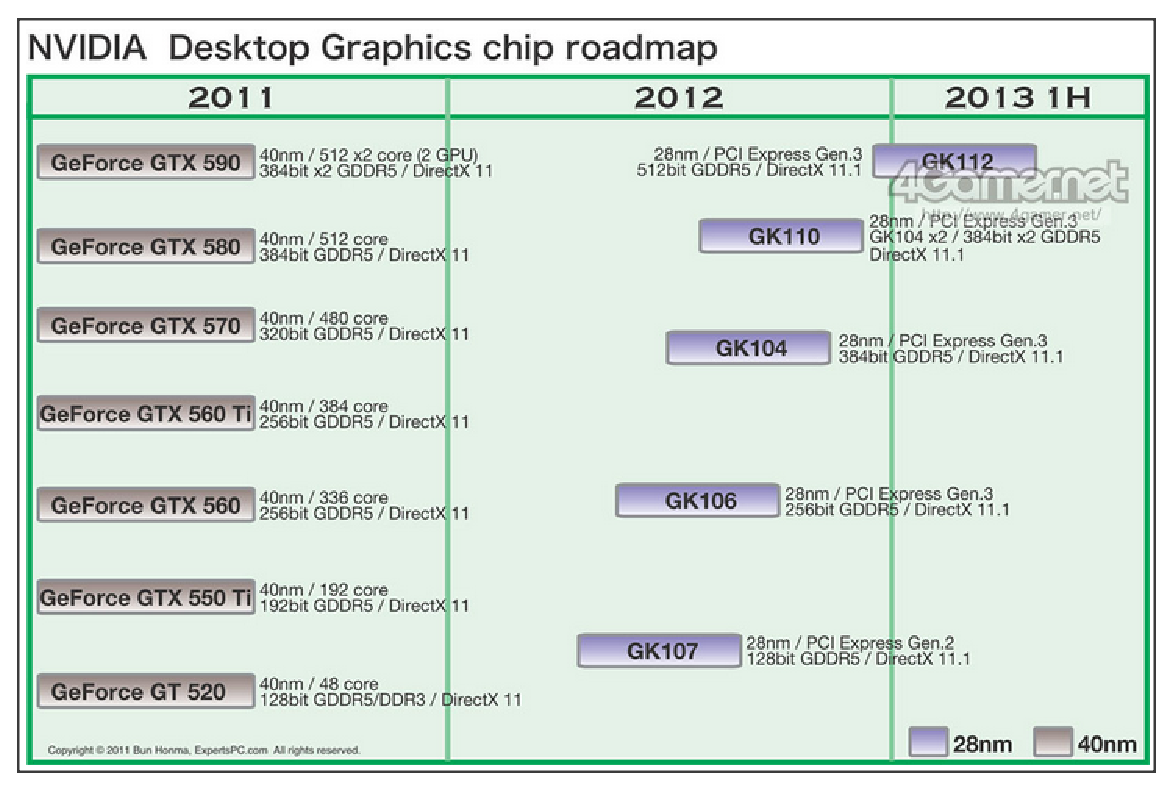
\includegraphics[height=7cm,
    angle=0]{./images/kepler_roadmap.eps}}
  \caption{Roadmap of Kepler 28nm technology}
  \label{fig:kepler_roadmap}
\end{figure}


\section{Kepler GPUs}

A good comparison between GPU chips is given in
Fig.\ref{fig:compare_CUDA-capable-GPUchips}.

\url{http://www.tomshardware.com/reviews/geforce-gtx-680-review-benchmark,3161-2.html}

\begin{figure}[hbt]
  \centerline{\includegraphics[height=5cm,
    angle=0]{./images/CUDA_GPU_comparison.eps}}
  \centerline{\includegraphics[height=5cm,
    angle=0]{./images/Compare_GTX680_GTX580.eps}} 
  \caption{GPU comparison}
\label{fig:CUDA_GPU_comparison}
\end{figure}

\subsection{GK104}
\label{sec:GK104}

{\bf GK104} is the first GPU chip based on the Kepler architecture to run on
PCIe Gen3. GK104 chip is designed for performance GPU, targers to mid-end users.
GK104 has
\begin{itemize}
  \item  3.54 billion transistors on 294 mm$^2$ die with 8 SMX, each with
192 CUDA cores, i.e. totally 1536 CUDA cores.
  \item PCI-e Gen3 (44 mm$^2$)
  \item 256-bit memory bus (60 mm$^2$)
  \item 4 GPC (each 37 mm$^2$)
  \item one GigaThread (6 mm$^2$)
  \item 512 KB L2 cache + 32 ROPs (37 mm$^2$)
  
  \item GRAPHICS: 80-96 texture units (TMUs). 
  \item The base clock is 915 MHz, which can be boost to
1010 MHz (using Turbo Boost 1.0), and memory clock 6.008 GHz GDDR5.
Expected performance: more than 2TFLOPs in single-precision. 

  \item GK104 requires CUDA 3.0 minimum. 
  
  \item The fraction of FP64 is 1/24 FP32.
\end{itemize} 
The first videocard product to use GK104 is Geforce GTX 680 with 2
GB 1.502 GHz RAM, running at 1006 MHz (boost to 1058 MHz). Using the formula in
Sect.\ref{sec:chip-memory}, the peak theoretical data throughput is 192 GB/s.  


% with 640-768 CUDA cores; memory interface 256-bit or 384-bits.

There are variants of GK104, i.e. the cut-down versions: {\bf GK104-335-A2} with
7 SMX (1344 CUDA cores, 256-bit memory bus, 112TMU, 32 ROPs), {\bf GK104-400-A2}
with 6 SMX (192-bit memory bus), {\bf GK104-425-A2}.
The videocards Geforce GTX 670 use GK104-335-A2, 2GB GDDR5, core-clock 915-950
MHz, memory clock 1.25 GHz.
\footnote{\url{http://www.tweaktown.com/news/23836/nvidia_preps_two_more_kepler_gk_104_based_cards_gtx_660_and_670/index.html}}
The videocards Geforce GTX 680 use GK104-400-A2.
The videocards Geforce GTX 770 use GK104-425-A2 (425 implies some slight
optimisation and changes).

Geforce GTX 690 was first available around May-2012, a videocard combining two
fully-enabled GK104-chips interconnected using SLI, giving total 2x1536 CUDA
cores, 2x128 TMUs, 2x32 ROPs, FP64 units (is about 1/24 FP32 units). GTX 690 TDP
is 300 watts.

GK104 has
\begin{enumerate}
  \item PCI-e Gen3 Host Interface
  \item 4 256-bit memory controllers
  \item 4 GPC with each GPC has 2 SMX block. So, totally it has 8 SMX blocks.
  XMS runs at the base-clock. 
  \item L2 cache shared by all CUDA cores.
  \item With 4 memory controller, GK104 has 4x128=512KB L2-cache and 32 ROP units. It
means it can do 32 color samples at once. 
\end{enumerate}




\subsection{GK107}
\label{sec:GK107}

GK107 chip is for entry GPU with PCI-e Gen2 and uses 1.3 billion transistors. 
GK107 has only 2 SMX units (giving totally 384 CUDA cores). GK107 has 32 texture
units and 16 ROPs. The memory bus is 128-bit (support DDR3 and GDDR5 memory).
Base-clock is 900 MHz, and memory clock is 900 MHz. The chip's TDP is 65 watts (i.e. no
external power connection is required).

The first videocard to use GK107 chip is GeForce GT 640 (1GB DDR3).

\subsection{GK106}

GK106 is built on 210 mm$^2$ die. Its memory bus is 192-bit (GDDR5 memory
interface). GK106 features 2 raster engines (RPC), 4 SMX (i.e. 768 CUDA cores),
24 ROPs, and 64 TMUs. The base-clock is 1006 MHz, and can be boost to 1359 MHz.
 
The first videocard to use GK106 chip is GeForce GTX 660 with TDP
130 watts (Sept-2012).



\subsection{GK110 (flagship), GK110b}
\label{sec:GK110}
\label{sec:GK110b}

Unlike Fermi-based GPU family whose flagship GPU chip is GF100, in Kepler, the
flagship GPU chip is GK110 (not GK100) which is considered a 28nm version of
GF110 (a major revision of GF100). {\bf GK110 requires minimum CUDA 3.5}
instruction sets (Sect.\ref{sec:CC3.5}).

Even though GK104 is powerful (Sect.\ref{sec:GK104}), it's not designed for
general-purpose computing, i.e. no ECC memory protection, very low (only 1/24)
FP64/FP32 rate, few load/store units in comparison to ALU (CUDA cores), low L1
bandwidth per ALUs (0.33 Byte/FLOP for 32-bit operations, 0.66 Byte/FLOP for
64-bit operations)
\footnote{\url{http://www.ilsistemista.net/index.php/hardware-analysis/27-big-kepler-gk100-speculations.html}}

A complete GK110 GPU has 
\begin{itemize}
  \item  about 550 mm$^2$, with total 7.1B transistors. 
  
  GK110 can accommodate 15 SMX units (Sect.\ref{sec:SMX} - an extension concept
  from SM (streaming multiprocessor)). However, only 14 SMX are
  activated, as one SMX is disabled, giving total 14x192 = 2,688 CUDA cores
  and 14x16=224 TMUs available (NOTE: GTX 680 has 128 TMUs). 
  
  The variant GK110-301-B1 ({\bf GK110b}) is the GPU chip (having a larger die
  561 mm$^2$ and 7.08 billion transistors) with full 15 SMX units, i.e.
  giving total 2880 CUDA cores. GK110B is being used to build Tesla K40
  (Sect.\ref{sec:K40}).


  \item FP64/FP32 ratio is 1/3: Every 3 CUDA cores has 1 FP64 double-precision
  unit. FP64 in GK110 can do $> 1$ TFLOPs.

So, in an SMX, it has 192*1/3=64 DP units. With this ratio, GK110 can deliver
power of calculation in double-precision about 50\% - 85\% compared to power in
single-precision (FP32).
\footnote{\url{http://technewspedia.com/more-details-of-nvidia-tesla-cgpu-k20-gk110/}}
  
  \item memory interface: 384 bits
  
  \item connect to motherboard using PCI-e Gen2
  
  \item GK110 has 1.5MB L2 cache, with the number of 32-bit register per SMX is 65,536.

Compared to GF100 (Sect.\ref{sec:gf100-fermi}, the number of cores is 6x, while
the number of registers only double. So, it's important to limit the number of
registers/thread when writing CUDA kernels.
  
\end{itemize}


To improve performance per watt, the clock is down from 2x in Fermi to 1x clock
in Kepler.
\begin{verbatim}
For login: area is 1.0x, power is 1.0x
   Kepler: 1.8x and 0.9x
For clocking: area is 1.0x, power is 1.0x
   Kepler: 1.0x and 0.5x
\end{verbatim}
This show how they do power saving.

Selections:
\begin{enumerate}
  
  \item Geforce GTX Titan (Feb 2013) is the first videocard to use GK110 chip.
  It uses 6 GB of memory. Tesla K20 is using GK110 (Sect.\ref{sec:K20}).

  \item GeForce GTX 780Ti is the first videocard (Sep-2013) to use GK110b chip,
  yet with reduced double-precision.
  
GeForce GTX 780 Rev. 2 also use GK110b, yet has some shading units disabled,
i.e. only 2304 shading units (CUDA cores, running at 863 MHz, which can be
boosted up to 902 MHz), 192 TMUs (texture mapping units) and 48 ROPs, and
3,072MB 1502 MHz GDDR5 memory interconnected using 384-bit memory interface.

  \item 
\end{enumerate}


\subsection{GK100/GF112}

SUMMARY: GK100/GK112 has 1024 CUDA cores, with 512-bit GDDR5 Memory interface;
memory bandwidth ??? GB/s. GRAPHICS: 128 textures units (TMUs), 64 raster operators
(ROP). Performance:

\subsection{GK20A}
\label{sec:GK20A}

GK20A is the Kepler-based graphics core found within the Tegra K1 SoC
(Sect.\ref{sec:Tegra_nvidia}). GK20A has 192 GPU cores. In addition to the GPU
chip, Tegra K1 also features either a 64-bit ARM or Nvidia's Project-Denver
processor. Project-Denvor process is now called 32-bit quad-core, 4-Plus-1
Cortex-A15
processor.\footnote{\url{http://www.phoronix.com/scan.php?page=news_item&px=MTU2MDg}}

\subsection{GK210}
\label{sec:GK210}

GK210 is the third revision of GK110 (Sect.\ref{sec:GK110}). There are major
feature changes, Fig.\ref{fig:GK110_mainstreams}. Even though the memory bus
interface do not change (i.e. 384-bit memory interface), it has
\begin{enumerate}
  \item only 13 SMX are activated, i.e. giving total 2496 cores
  
  \item each SMX (Sect.\ref{sec:SMX}) has
  \begin{itemize}
 
    \item double the registers (compared to GK110, GK110b): 512KB registers,
   i.e.   131,072 32-bit registers.
  
    \item double shared-mem/L1 cache (compared to GK110, GK110b): 128KB total 
  
  \end{itemize}
\end{enumerate} 
The small change here improves the data throughput within an SMX,
serving to improve efficiency and keep the CUDA cores working more often. 

\begin{figure}[hbt]
  \centerline{\includegraphics[height=5cm,
    angle=0]{./images/GK110_mainstreams.eps}}
  \caption{The mainstream GPU for Tesla Kepler chip}
  \label{fig:GK110_mainstreams}
\end{figure}

The new GK210 is being used to produce Tesla Kepler K80 (Sect.\ref{sec:K80}).



\section{non-Tesla Kepler-based products}
\label{sec:Kepler-non-Tesla}

For Kepler-based Tesla products, see Sect.\ref{sec:Tesla-Kepler}.

\subsection{-- Geforce 600, 700}
\label{sec:Kepler-based-Geforce}

Geforce 600 series use GK104, GK106, GK107 and GK208.

Geforce 700 series use GK107, GK110, GK208 and GM107 (Maxwell). 

Geforce GTX Titan and Geforce GTX 780 were released in 2013. In GTX Titan
(Black), double-precision can be either 1/3 or 1/24 of single-precision
depending on the user-selected configuration. Other Kepler's GPU,
double-precision performance is fixed 1/24 of single precision. Geforce 700
series double precision performance is 1/32 of single-precision
performance.\footnote{\url{http://www.anandtech.com/show/7764/the-nvidia-geforce-gtx-750-ti-and-gtx-750-review-maxwell/5}}

\begin{figure}[hbt]
  \centerline{\includegraphics[height=5cm,
    angle=0]{./images/compare_CUDA-capable-GPUchips.eps}}
\caption{Compare GF100, GF104, GK110, and GK104
\footnote{\url{http://www.tomshardware.com/reviews/geforce-gtx-titan-gk110-review,3438-2.html}}}
\label{fig:compare_CUDA-capable-GPUchips}
\end{figure}

\subsection{-- Quadro K5000, K6000}
\label{sec:Kepler-based-Quadro}

Quadro K5000 is first Kepler-based Quadro GPU, successor to Fermi-based Quadro
5000 (Sect.\ref{sec:Fermi-based-Quadro}). Quadro K5000 uses GK104 chip
(Sect.\ref{sec:GK104}); while Quadro K6000 uses GK110 chip
(Sect.\ref{sec:GK110}).

\begin{figure}[hbt]
  \centerline{\includegraphics[height=5cm,
    angle=0]{./images/Quadro-Kepler.eps}}
  \centerline{\includegraphics[height=5cm,
    angle=0]{./images/Quadro2-Kepler.eps}}
  \caption{Compare between Kepler-based Quadro (K5000) vs. Fermi-based Quadros
  (Quadro 6000 and 5000)}
\label{fig:Quadro-Kepler}
\end{figure}

Quadro K6000 is the second-line Kepler-based Quadro GPU, successor to
Fermi-based Quadro 6000 (Sect.\ref{sec:Fermi-based-Quadro}). 



\section{Tesla Kepler board}
\label{sec:Tesla-Kepler}

For Kepler-based non-Tesla products, see Sect.\ref{sec:Kepler-non-Tesla}.

There are 3 early members in the Tesla-Kepler family GPGPU card (board),
Fig.\ref{fig:Tesla_Kepler_comparison}. Now, there is a new one: Tesla K80
(Sect.\ref{sec:K80}).

\begin{figure}[hbt]
  \centerline{\includegraphics[height=5cm,
    angle=0]{./images/Tesla_Kepler_comparison.eps}}
  \caption{Technical specification for Tesla Kepler}
  \label{fig:Tesla_Kepler_comparison}
\end{figure}

\subsection{Tesla K10}
\label{sec:K10}

Tesla K10 is optimized for single-precision, using two GK104 chip
(Sect.\ref{sec:GK104}), which can deliver 2x performance compared to Tesla M2090
GPU for single-precision applications.

\subsection{Tesla K20 (K20m, K20c) and Tesla K20X}
\label{sec:K20}

Tesla K20 are designed for double-precision (DP64), based on GK110 chip
(Sect.\ref{sec:GK110}), with 320-bit memory interface. 

Tesla K20 has less CUDA cores, i.e. 2496, and use 5.2GHz 5GB GDDR5 memory
of 320-bit memory interface giving 208 GB/s. Tesla K20X is a minor revision with
14 SMX activated and 5.2GHZ 6GB GDDR5 memory of 384-bit memory interface giving
250 GB/s.

\begin{itemize}
  \item K20X (with 14 SMX, i.e. 2688 CUDA cores): 3.95 TFLOPs on
  single-precision and 1.31 TFLOPs on double-precision
  
Passive heatsink relies on chassis cooling of specially-designed GPU servers  
It has 235W TDP.
  
  \item K20 (with 13 SMX): 3.52 TFLOPs on single-precision and 1.17 TFLOPS on
  double precision.

Passive (K20m) or active (K20c) heatsink options for servers and workstations
It has 225W TDP.

\end{itemize}
\url{https://www.microway.com/hpc-tech-tips/nvidia-tesla-k20-gpu-accelerator-kepler-gk110-up-close/}

\subsection{Tesla K40}
\label{sec:K40}

Tesla K40 was introduced in SC'2013 conference as the first fully-enabled Kepler
Tesla card. It is based on GK110B variant of NVIDIA's GPU
(Sect.\ref{sec:GK110}). Tesla K40 is designed for large-scale double-precision
simulation, which has 12 GB of {\bf 6GHz GDDR5 memory} (memory bandwidth is 288
GB/s, Fig.\ref{fig:Tesla_K40_benchmark}), and full 15 SMX units, i.e. 2880 cores
that can deliver 4.29 TFLOPs for single-precision and 1.43 TFLOPs on
double-precision.

\begin{mdframed}

Memory bandwidth of 288GB/s
 \footnote{\url{http://www.pcper.com/news/General-Tech/NVIDIA-Tesla-K40-GK110b-Gets-Career-and-more-vRAM}},
is 50\% higher than GTX 680 2GB and about the same as ATI/AMD HD 7970 3GB.

\end{mdframed}

\begin{figure}[hbt]
  \centerline{\includegraphics[height=5cm,
    angle=0]{./images/Tesla_K40_benchmark.eps}}
\centerline{\includegraphics[height=5cm,
    angle=0]{./images/Tesla_K40_benchmark2.eps}}    
  \caption{Brief overview of K40}
  \label{fig:Tesla_K40_benchmark}
\end{figure}

Since Tesla K40, the GPU Boost 2.0 is added which was previously only available
in Geforce cards as GPU Boost 1.0, Fig.\ref{fig:GPU_Boost}. Tesla 40 base clock
is 745 MHz, and can jump to 2 different boost clock: 810 MHz or 875 MHz. K40 can
deliver 20-40\% increase in performance in some applications compared to K20.
There are certain limitations to GPU Boost 2.0. Tesla K40 had to obey its TDP
(235W TDP), but operators could select which of 3 clockspeeds they wanted,
picking the one that comes closest to (but not exceeding) TDP for the best performance. The GPU
Boost in Tesla K80 is better (Sect.\ref{sec:K80}).

\begin{figure}[hbt]
  \centerline{\includegraphics[height=3.5cm,
    angle=0]{./images/GPU_Boost.eps}}
  \caption{GPU Boost 2.0 can automaticaly scale up frequencies based on
  voltage, temperature and power target}
  \label{fig:GPU_Boost}
\end{figure}

\subsection{Tesla K80}
\label{sec:K80}

Tesla K80 has been introduced at SC'2014 conference,
Fig.\ref{fig:Tesla_K80_comparison}. It is a dual-GPU card using two GK210
(Sect.\ref{sec:GK210}), thus doubles the number of transistors, i.e. 2 x 7.1B,
compared to GK110. 

\begin{mdframed}
Using dual cards has been done before (Tesla K10, or GeForce Titan Z), but this
is different as only 13 out of 15 SMX are enabled on each GPU, i.e. giving the
combined  4,992 CUDA cores enabled. 

The GK210 chip in Tesla K80 operates at 562MHz (normal) and 875MHz (boost
state). This allows Nvidia to put two high performance GPU chips within 300W TDP
(i.e. 150W per GPU system) is no small achievement in and of itself, though for
this reason GPU Boost plays a big part in making the overall product viable.
The worst case scenario is that it's only 2\% more energy efficient than K40
(Sect.\ref{sec:K40}) while the best case is 59\%, with the realistic case being
somewhere in the middle.
\end{mdframed}


Tesla GK80 specs:
\begin{enumerate}
  
  \item  The FP64/FP32 ratio is still 1/3: but with more cores, it can deliver
  8.74 TFLOPS in single and 2.91 TFLOPS in double precision,
  Fig.\ref{fig:Kepler_performance}.

Compared to Tesla K40 (Sect.\ref{sec:K40}) this is roughly 74\% faster; though
GPU Boost means that the real performance advantage will not be that high.
This puts the clockspeed at a range of 562MHz to 870MHz, i.e. turned down
slightly from Tesla K40. Tesla K80 NVIDIA has now implemented a full and dynamic
GPU boost implementation; just as in their consumer cards, the card will clock
itself as high as the TDP will allow.


  \item Each GK210 has 12GB 5GHz GDDR5 ECC-enabled memory of 384-bit memory
  interface (giving 240 GB/s bandwidth on each chip), giving total 24GB or
  480GB/s bandwidth in total.
\begin{verbatim}
12GB RAM--GK210------PLX------- GK210--12GB RAM
                     |
                    |
                 PCI-e Gen3
\end{verbatim}

% Tesla K80 also double the memory (with 24GB), i.e. each GPU has 12GB of GDDR5 at
% clocked 5GHz, i.e. 240GB/sec memory bandwidth per GPU. It means the total
% bandwidth among the two GPU is 480GB/sec.
    
    
    \item Passive heatsink relies on chassis cooling of specially-designed GPU servers  
    
\end{enumerate}
\url{http://www.anandtech.com/show/8729/nvidia-launches-tesla-k80-gk210-gpu}

\textcolor{red}{Strictly speaking, Tesla K80 is often but not always superior to
Tesla K40}.
Per GPU throughput is lower than on Tesla K40, so given a task that doesn't scale
well over multiple GPUs a Tesla K40 could still be faster. 


\begin{figure}[hbt]
  \centerline{\includegraphics[height=5cm,
    angle=0]{./images/Tesla_K80_comparison.eps}}
  \caption{Comparison Tesla K80 with other Tesla Kepler cards}
  \label{fig:Tesla_K80_comparison}
\end{figure}
 

\begin{figure}[hbt]
  \centerline{\includegraphics[height=5cm,
    angle=0]{./images/Kepler_performance.eps}}
  \caption{Performance comparisons (Kepler GPUs vs. Intel CPUs)}
  \label{fig:Kepler_performance}
\end{figure}

Other products:
\begin{enumerate}
  \item Cray CS-Storm: 8 K80 per node
  \item Dell C4130: 4 K80 per node
  \item HP SL270: 8 K80 per node
  \item Quanta S2BV: 4 K80 per node
\end{enumerate}
\url{http://www.anandtech.com/show/8729/nvidia-launches-tesla-k80-gk210-gpu}
 
\section{New features}

The number of fixed-function logic is 32 ROPs (raster operation units) and 128
TMUs (Texture Memory Units). The memory is set at 1.25 GHz in quad-data rate, a
25\% boost over GF100/GF110. 

The GeForce run double-precision with one-sixth rate, and Quadro/Tesla run with
half rate of single-precision.

\begin{figure}[hbt]
  \centerline{\includegraphics[height=7cm,
    angle=0]{./images/Kepler_gpus.eps}}
  \caption{Kepler GPUs information}
  \label{fig:kepler_gpus}
\end{figure}

There are two main models: GK110 (image processing) and GK120 (double-precision
3x, high-performance computing). GK110 has more than 3000 cores.
The successor to GTX560 is GK104, with as many as 768 cores (or shader units),
i.e. 50\% higher than GTX580 with 512 cores. 


The shader clock also increase to 1600 MHz, giving 2.46 TFLOPs. Variations
include 640 cores with higher clock rates, or 704 cores with 1600 MHz. The first
generation of Kepler, GK107, will be available in March, 2012.

The architecture of GK104 is similar to GF110. However, it has 1536 streaming
processors (SPs), rather than 512. Each SM in GK104 is composed of 16x6=96 SPs,
rather than 32 in Fermi, and 8 in Tesla. Similar to GF110, each GPC is composed
of 4 SMs in GK104. So, different model of Kepler-based GPUs will have 96 (1SM),
384 (1 GPC), 768 (2 GPCs), 1536 (4 GPCs), and 2304 (6 GPCs) cuda cores. The
memory controller then comes with different bandwidths: 64-bit, 128-bit,
192-bit, 256-bit, 320-bit and
512-bit\footnote{\url{http://www.brightsideofnews.com/news/2012/2/10/real-nvidia-kepler2c-gk1042c-geforce-gtx-670680-specs-leak-out.aspx}}.


\subsection{GPC}
\label{sec:Kepler_GPC}

Like Fermi, the high level hardware block is GPC (Graphics Processing Cluster)
in Kepler, with its own hardware resources for rasterization, shading,
texturing, and compute. 

GK104 chip has 4 GPC, each GPC has
\begin{enumerate}
  \item 1 Raster Engine (Sect.\ref{sec:raster_engine})
  \item 2 SMX (Sect.\ref{sec:Kepler_SMX})
\end{enumerate}

GK110 chip has 5 GPC, each GPC has
\begin{enumerate}
  \item 1 Raster Engine (Sect.\ref{sec:raster_engine})
  \item upto 3 SMX (Sect.\ref{sec:Kepler_SMX}), i.e.  GK110 in GTX Titan
  videocard isn't fully implemented (the fifth GPC has only 2 SMX); only Tesla
  K20 has full 5 GPCs, each with 3 SMX, giving totally 2,880 CUDA cores. 

\end{enumerate}

GTX 680 has 4 GPCs, i.e. 8 SMX giving the total 1536 CUDA cores, and can perform
32 pixels per clock (i.e. 32 single-precision instructions per clock),
Fig.\ref{fig:GTX680_GK104}.

\begin{figure}[htb]
  \centerline{\includegraphics[height=5cm]{./images/GK104_GTX680.eps}}
  \caption{GTX 680 block diagram}
  \label{fig:GTX680_GK104}
\end{figure}


\subsection{SM to SMX}
\label{sec:SMX}

Check.

Again, most of the key hardware units for graphics processing reside in the SM.
A major change in Kepler-based GPU is the concept of {\bf SMX} (Shader
Multiprocessor, Shader Multiprocessing Engine), rather than using SM (streaming
multiprocessor), Fig.\ref{fig:Kepler_SMX}. Each SMX has 
\begin{itemize}
  \item 192 single-precision CUDA cores (FP32 units or shader ALUs), 32
  double-precision units (FP64)
  
  \item 32 special function units (SFU), 
  
  \item 1 I-cache, 
  
  \item 1 uniform cache (read-only constant), 
  
  \item 64KB shared/L1-cache memory (Sect.\ref{sec:Kepler_L1cache}), 
  
 This number is doubled, i.e. 128 KB for SMX in GK210 (Sect.\ref{sec:GK210})
  
  \item 1 Texture cache (now can be used as read-only data cache in Kepler), 

   \item 65,536 32-bit registers file (Sect.\ref{sec:Kepler_registers}),

This number is doubled, i.e. 131,072 32-bit registers for SMX in GK210
(Sect.\ref{sec:GK210})

   \item 4 warp schedulers (Sect.\ref{sec:Kepler_warpscheduler}),

   \item 8 instruction dispatch units (Dispatch),
   
   \item 16 TEX units (TMUs), 
   
   \item 1 PolyMorph Engine version 2.0
   (Sect.\ref{sec:polymorph-unit-+}) and 
   
   \item 32 load/store units (LD/ST).
\end{itemize}

Math operations fully compliant to IEEE 754-2008
standard for single-, double-precision and fused multiply-add (FMA) operations.
Compared to Fermi's SM, an SMX has 8x number of SFU, 6x single-precicion cores,
2x double-precision units. As 32 SP instruction are issued per clock.
\begin{itemize}
  \item four warp scheduler (only two in Fermi)
  \item 8 dispacht units (from 4 in Fermi)
  \item 16 texture units (from 8 in Fermi)
  \item 65,536 32-bit register files (double from Fermi)
  
\end{itemize}



\begin{framed}
In Fermi, each SM has 32 SPs (GF100 chip) or 48 SPs (GF104 chip) + 4 SFUs + 1 MT
issue + 1 I-cache + 1 uniform-cache (replacement for C-cache) + 64KB shared-memory/L1
cache + \textcolor{red}{12KB Texture-cache} + 32K 32-bit
registers + 2 WARP schedulers + 2 Dispatch Units + 4 TEX units + 1
PolyMorph Engine + 16 load/store (LD/ST) units.

\end{framed}

Kepler GK110's SMX increases 8x the number of SFUs compared to Fermi GK110's SM.
\begin{figure}[hbt]
  \centerline{\includegraphics[height=5cm,
    angle=0]{./images/Kepler_Fermi_compare_SM.eps}}
  \caption{Compare at chip level between Fermi SM and Kepler SMX}
  \label{fig:SMX_SM}
\end{figure}

As we can see in Fig.\ref{fig:SMX_SM}, per-clock throughput for key graphics
operations are increased, e.g. FMA32, SFU, texture operations. 

GK104 chip (GTX 680): GTX 680 has 4 GPCs (Sect.\ref{sec:Kepler_GPC}) and 4
memory controllers. Each memory controller has 128 KB L2-cache (which is the
same in Fermi) and 8 ROP units. Thus, GTX 680 has total 128x4=512 KB L2-cache
and 32 ROP units. Compared to Fermi, the total L2-cache is less (512KB vs.
768KB). However, the GTX 680's L2-cache hit bandwidth has increased by 73\%.
  
\begin{figure}[hbt]
  \centerline{\includegraphics[height=2cm,
    angle=0]{./images/L2cache_Kepler.eps}}
  \caption{L2-cache in Kepler vs. Fermi}
\label{fig:L2cache_Kepler}
\end{figure}


\begin{figure}[hbt]
  \centerline{\includegraphics[height=5cm,
    angle=0]{./images/GK110_chipblock.eps}, \includegraphics[height=8cm,
    angle=0]{./images/Kepler_SMX.eps}}
  \caption{(A) GK110 chip block diagram; (B) Nvidia Kepler SMX}
  \label{fig:Kepler_SMX}
\end{figure}


\subsection{Grid Management Unit (GMU)}
\label{sec:Grid-Management-Unit-Kepler}
\label{sec:GMU-Kepler}

Kepler GK110 introduces the Grid Management Unit, which creates multiple
hardware work queues to reduce or eliminate false dependencies (Sect.\ref{sec:CUDA-stream}).

With the GMU, streams can be kept as individual pipelines of work.

There are 1000s of pending grids that are formed from the Stream Queue Managements, and then given to GMU.

Combined GMU with Hyper-Q (Sect.\ref{sec:Hyper-Q}),  the Work Distributor on
Kepler GPU can handle 16 active grids in parallel.
These components provide dynamic parallelism
(Sect.\ref{sec:dynamic-parallelism}).


\url{http://developer.download.nvidia.com/compute/DevZone/C/html_x64/6_Advanced/simpleHyperQ/doc/HyperQ.pdf}

\subsection{Shared/L1 cache}
\label{sec:Kepler_L1cache}

64KB shared/L1 cache can be configured in three ways (Fermi only use two ways)
\begin{enumerate}
  \item 16/48
  \item 48/16
  \item 32/32 (new)
\end{enumerate}

In Kepler (CC 3.x), the shared memory has 32 banks (Sect.F.5.3 CUDA C
programming book), each bank has bandwidth 64-bits per clock cycle. The bank can
resolve conflict only if threads in the same warps access the same 64-bit
segment. To take full advantage of it, we need to do 8-byte read.
Memory banks are twice as wide that in Fermi. Thus, Kepler is configurable
whether successive 32-bit words or successive 64-bit words should be assigned to
successive banks. This can be configured in \verb!cudaDeviceSharedMemConfig()!
from the host prior to launching your kernel, and specifying one of 
\begin{verbatim}
cudaSharedMemBankSizeDefault, 
cudaSharedMemBankSizeFourByte 
cudaSharedMemBankSizeEightByte
\end{verbatim}
\begin{enumerate}
  \item  In 8-byte configuration: Bank conflict occurs when two or more threads in a warp
request different 64-bit words from the same bank. \textcolor{red}{This is the
option when using double-precision}, an improvement over Fermi where
accessing a double-precision values always cause bank conflict. If shared memory
is the bottle neck in Fermi, then the new shared memory configuration can help
improve the performance.
  
Example:
\begin{verbatim}
Kernel  Execution Time
32-bit Shared Memory  2.1387 (ms)
64-bit Shared Memory (cudaSharedMemBankSizeFourByte)  1.78614 (ms)
64-bit Shared Memory (cudaSharedMemBankSizeEightByte)  1.33753 (ms)
\end{verbatim}  

  \item In 4-byte configuration: Bank conflicts occur if two or more threads in
  a warp access 32-bit words from the same bank where those words span multiple
  64-word aligned segments 
\end{enumerate}
\url{http://www.acceleware.com/blog/maximizing-shared-memory-bandwidth-nvidia-kepler-gpus}

\begin{mdframed}
Shared memory on Fermi has 32 banks, yet the bandwidth each bank is 32-bit per
clock cycles. Thus, successive 32-bit words are assigned to successive banks.
\end{mdframed}

In Kepler (CUDA CC 3.x), L1 cache is only and just only used for register
spills. L1 cache is always read fully coalesced by the warp since every thread
accesses its own word in the cache line. 

\begin{mdframed}
L1 cache is different in Fermi, with a quite traditional use of L1 cache, to
backing up global memory and cached in L2. So, threads can access efficiently L1 in an
uncoalesced manner.

An interesting behavior is that Fermi SM 2.0 L1 access has significantly lower
performance than Fermi's shared memory access, even though it's using the same
hardware. Fermi SM 2.1's L1 performance is comparable to shared.
\end{mdframed}
\url{https://devtalk.nvidia.com/default/topic/476667/cuda-programming-and-performance/why-texture-memory-is-better-on-fermi-/post/3401148/#3401148}
\url{https://devtalk.nvidia.com/default/topic/540044/question-on-the-l1-caching-of-the-gk-110/}


\subsection{Warp scheduler}
\label{sec:Kepler_warpscheduler}

The warp scheduler in Kepler is the simple software-based, not the
complex hardware-based like in Fermi. With software scheduling, the warp
scheduling was moved to Nvidia's compiler.

The Kelper warp scheduler select 4 warps, and 2 independent instructions per
warp to dispatch each cycle (as each warp scheduler has dual instruction patch
units), Fig.\ref{fig:Kepler_warpscheduler}.
Better than Fermi, Kepler allows double-precision instructions to be paired with
other instructions.


\begin{figure}[hbt]
  \centerline{\includegraphics[height=5cm,
    angle=0]{./images/Kepler_warpscheduler.eps}}
  \caption{Nvidia Kepler warp scheduler}
  \label{fig:Kepler_warpscheduler}
\end{figure}


\subsection{Texture handling}
\label{sec:Kepler_texture-handling}

To work with texture memory (in graphical applications), the previous approach:
textures are bound by a particular CPU to a particular slot in a fixed-size
table before GPU could reference them. The limitation with this approach: (1)
table size is fixed, the maximum textures to be used at a time is limited by the
size of the table, (2) CPU is doing unnecessary work, i.e. it has to load each
texture, and bind each texture loaded in memory to a slot in the binding table.

Kepler has a new form of texture handling known as blindless textures where the
two limitations above are remmoved. Here, the GPU can access any textures loaded
in the memory.


References:
\begin{enumerate}
  \item
  \url{http://www.techpowerup.com/155727/NVIDIA-GeForce-Kepler-Roadmap-Compiled.html}
\end{enumerate}

\subsection{Memory architecture}

Fermi, e.g. GeForce GTX 580 employs 1002 MHz memory clock. In Kepler,
the memory clock is revamped to 60008 MHz data rate.

GTX 680 (GK104) has total 4 memory controllers with 4 GPCs
(Sect.\ref{sec:Kepler_GPC}). So, with one memory controller per GPC, each memory
controller has 128KB L2-cache, eight ROP units (Sect.\ref{sec:rop}). Each ROP
unit process a single color channel in graphical applications. So, a full GTX
680 has 512 KB L2 cache and 32 ROPs.

\begin{enumerate}
  \item Geforce GK107: 128-bit GDDR5 memory interface, PCI-e 2.0
  \item GK106, GK104, GK110: use PCI-e 3.0
  \begin{itemize}
    \item GK106: 256-bit GDDR5 memory interface, to replace GTX 560.
    \item GK104 (highest performance of single GPU): 384-bit GDDR5 memory
    interface, 1.5GB or 3GB memory. With more than 2 TFLOPs single-precision FP,
    it gives 60\% higher than GTX560 (1.26 TFLOPs), and 30\% higher than GTX580
    (1.58 TFLOPs).
    \item GK110 (dual GPU): combine 2 GK104, i.e. 384-bit x2  GDDR5 memory
    interface. This can yield more than 4 TFLOPs
  \end{itemize}
  \item (Plan 2013) GK112: support massive 512-bit GDDR5 memory interface
\end{enumerate}

\subsection{Registers}
\label{sec:Kepler_registers}

With 65,536 32-bit registers per SMX, it is double compared to that in Fermi's
SM. Fermi limit 63 registers per thread: a common Fermi performance limiter and
leads to excessive spilling. Kepler alows up to 255 registers per thread (new
ISA encoding), especially helpful for FP64 apps. This makes Kepler a better
choice for codes that exhibit high register pressure and can avoid spilling
behavior.

Example:QCD fp64 sample runs 5.3x faster as spilles are eliminated with extra
registers. \textcolor{red}{We may need to readjust maximum registers in our
spatial cell modelling}.

% Codes that use many registers that experiences spilling behavior in Fermi can
% now see a speed-up as an increased in available per-thread register count.

\subsection{TXAA} 

TXAA is a new anti-aliasing method (for game engines) designed exclusively to
Kepler by Nvidia.

\subsection{Shuffle (exchange data between 2 threads)}

Fig.\ref{fig:Kepler_shuffle} shows how we can exchange data between 2 threads in
the same warps without using shared memory.


 \begin{figure}[hbt]
  \centerline{\includegraphics[height=5cm,
    angle=0]{./images/Kepler_shuffle.eps}}
  \caption{New shuffle instructions allows threads within a warp to exchange
  data}
  \label{fig:Kepler_shuffle}
\end{figure}


\subsection{Atomic operations}

Atomic operations have also been overhauled, with NVIDIA both speeding up the
execution speed of atomic operations and adding some FP64 operations that were
previously only available for FP32 data.


\section{Unified Memory (since Kepler (CC 3.0) with CUDA 6.0)}
\label{sec:Unified-Memory-CUDA6.0}

CUDA 6 on pre-Pascal GPUs (and device with compute capability 3.0+), adds one
extra layer of convenience to the CPU/GPU memory management task with the
introduction of Unified Memory (UM) which is a {\bf single} virtual memory
shared between processors (multiple GPUs, and CPUs on the same node).

\subsection{-- take-turns access with page fault}


REMEMBER that virtual memory is organized into multiple {\bf pages}, each page
points to a physical memory location (which can be on CPU or GPU) and two pages
can points to the same location. Each GPU/CPU has its own page table (but the
same page on each device are supposed to reference to the same data).
If the page does not point to a physical location, a {\bf page fault} occurs
\begin{verbatim}
            GPU-A                   GPU2
      page1 -> A's phys.mem      B'phys.mem      page1
                                            <--- page2 
                                                 page3 [*addr3=1] ->page fault
NOTE:
 When page1 is referenced to A's phys-mem then page1 in GPU2 must be NOT
      pointing to anything [i.e. only one data at a time]
\end{verbatim}
and the CUDA resolve this, i.e. retrieving the page, and then replay the data
access.
\begin{verbatim}
            GPU-A                   GPU2
      page1 -> A's phys.mem      B'phys.mem      page1
                                            <--- page2 
                                            <--- page3 [*addr3=1] ->retrieve and replay
\end{verbatim}
next, if in turns GPU-A access the data on page2 and page3, page faults occur on GPU-A
\begin{verbatim}
            GPU-A                   GPU2
          page1 -> A's phys.mem      B'phys.mem      page1
[*addr2=1]page2                                 <--- page2 
[*addr3=4]page3                                 <--- page3
\end{verbatim}
and pages data are migrated to GPU-A physical memory by CUDA driver, i.e.
 copy data from B's phys.mem to A's phys.mem before replay the data access
\begin{verbatim}
            GPU-A                   GPU2
          page1 -> A's phys.mem      B'phys.mem      page1
[*addr2=1]page2 ->                                   page2 
[*addr3=4]page3 ->                                   page3 
\end{verbatim}

{\bf MEMORY OVERSUBSCRIPTION}: When from GPU-A we access data that exceeds the
physical limit of memory on GPU-A, e.g. GPU-A can accomodate upto 4 pages of data
but we access to page5 (which points to GPU-A's phys.mem)
\begin{verbatim}

\end{verbatim}
then a page fault occurs, which trigger the data migration, i.e.
the data from one of the page (1 to 4) must be migrated to GPU-B, before data
from page-5 is migrated to GPU-A

\subsection{-- concurrent access}


\subsection{-- pre-Pascal GPU}

Kepler GPU releases the first support for Unified Memory. There is no change to
that in Maxwell GPU. The limits

\begin{enumerate}
  \item  No GPU page fault support: move all dirty pages on kernel launch
  
  \item No concurrent access, no GPU memory oversubscription, no system-wide atomics
\end{enumerate}



It offers 'single-pointer-to-data', that we can use from both host-side and
gpu-side code. This feature, from the user-perspective, seems similar to CUDA’s
zero-copy mapped memory (Sect.\ref{sec:zero-copied-memory}), i.e. eliminating
the need to explicitly define all data transfers between host and device memory,
yet the data are not limited to the pinned memory region.


CUDA has supported Unified Virtual Addressing (UVA - Sect.\ref{sec:UVA}) since
CUDA 4.0 on Fermi card (Sect.\ref{sec:fermi}), and while Unified Memory depends
on UVA, they are not the same thing. 
\begin{enumerate}
  
  \item With UVA, the single pointer (to be accessible from both GPU and CPU)
  must point to data on CPU shared-region called pinned memory
  (Sect.\ref{sec:pinned-memory}).
  
  \item UVA does NOT move data between CPU and GPU, and data always reside on
  CPU-side at pinned memory region. 
  
  UVA allocates memory on the host-side (within the page-locked memory whose
  size is Linux kernel-dependent, i.e. determined by the O/S).
\end{enumerate}

CUDA 6 creates {\bf a pool of managed memory} that is shared between the CPU and GPU,
bridging the CPU-GPU divide. Managed memory is accessible to both the CPU and
GPU using a single pointer.



The data, upon being used by either the host-side code or CUDA kernel, must be
migrated accordingly. This is however, done behind the scence by the CUDA
driver. The current limitation in CUDA 6's UM is that:
all data are copied from host-side to kernel-side, whenever a kernel is
launched, regardless whether that data is being used by the given CUDA kernel or
not. This is relaxed in CUDA 8.0 and Pascal GPU
(Sect.\ref{sec:Unified-Memory-CUDA8.0}).


CUDA 6's UM uses \verb!cudaMallocManaged()! (Sect.\ref{sec:cudaMallocManaged}) to
allocate the data [where: CPU or GPU?] that is eligible to be used by both
host-code and kernel-code.

Unified Memory offers a “single-pointer-to-data” model that is conceptually
similar to CUDA’s zero-copy memory, but it is NOT the same as data copy still
occurs and is done behind the scene.
\begin{enumerate}
  
  \item UVA's {\it zero-copy}: data is always allocated and resides on CPU-side
  
  Access to this data from GPU is done via PCI-e which is slow. 
  
  \item UM: data are moved between CPU and GPU RAM on demand, with a page (4KB)
  granularity. It's similar to manual copying before/after kernel call, but
  automatically managed by the CUDA.
  
   When data that can be potentially accessed by kernel (i.e. available for the
   stream to which the kernel belongs) are absent on GPU side, entire array is
   copied from CPU to GPU prior to kernel start.
   
   
Pascal and more recently GPUs can use on-demand copying with page granularity
for both cases (see above description), but ATM it is implemented only by Linux
(TCC?) driver.
  
  \item a single pointer, refereing to such memory location, is used on both sides
  
  So it never faster than manual memory management, sometimes may be slower
  (when automatic heuristics sucks), but simplifies the program.
  
\end{enumerate}

One key difference between the two is that with zero-copy allocations the
physical location of memory is pinned in CPU system memory such that a program
may have fast or slow access to it depending on where it is being accessed from.
Unified Memory, on the other hand, decouples memory and execution spaces so that
all data accesses are fast.

\begin{mdframed}

In a typical PC or cluster node today, the memories of the CPU and GPU are
physically distinct and separated by the PCI-Express bus. Before CUDA 6, that is
exactly how the programmer has to view things.

Also, data that is shared between the CPU and GPU must be allocated in both
memories, and explicitly copied between them by the program. This adds a lot of
complexity to CUDA programs

Thus, the use of the cudaHostAlloc and cudaMemcpy combination is no longer a
requirement. As far as the host is concerned, no distinction is made in terms of
accessing memory allocated with cudaMallocManaged or through malloc.

\url{https://devblogs.nvidia.com/unified-memory-in-cuda-6/}
\end{mdframed}


\textcolor{red}{What's happening behind the scence}:
The key is that the system automatically migrates data (i.e. copy to GPU, or
copy to CPU) allocated in Unified Memory between host and device so that it
looks like CPU memory to code running on the CPU, and like GPU memory to code
running on the GPU. The copy is managed by the system, and only occurs when the
data is accessed from host-code, i.e. if the data is accessed only by the
kernel, the there is no cudaMemcpy() occurs. 

As Unified Memory is able to automatically migrate data at the level of
individual pages between host and device memory, it required significant
engineering to build, since it requires new functionality in the CUDA runtime,
the device driver, and even in the OS kernel.



\textcolor{red}{What's good about UVA?}
\begin{enumerate}
  \item We can also declare a data as managed using \verb!__managed__! keyword
  \label{sec:__managed__-keyword}
  
  the \verb!__managed__! type qualifier that allocates, at compile time, a quantity stored in managed memory.
  
  
  \item For UM, the memory is allocated on the device and transparently made
  available where needed. Specifically, upon a call to
  
\begin{verbatim}
cudaError_t cudaMallocManaged(void** devPtr, size_t size, unsigned int flag);
\end{verbatim}  
the user has, in devPtr, a pointer to an address of a chunk of device memory.

A unified memory allocation physically takes place in device memory on the
device that happens to be active at the time of the allocation. When this memory
is operated upon by the CPU, the migration to host happens at page-level
resolution, which is typically 4KB. The runtime tracks dirty pages and detects page faults.

\textcolor{red}{Implicit data transfer between CPU and GPU}:
It transparently moves (over the PCIe bus) only the dirty pages. Pages touched
by the CPU (GPU) are moved back to the device (host) when needed.
 

This address can be equally well manipulated on the device and the host (though
MUST NOT be simultaneously).
That's why calling \verb!cudaDeviceSynchronize()! is very important after the
kernel calls, before using that data from the host.
ailure to obey this rule will lead to a segfault.

Example of segfault:
\begin{verbatim}
__device__ __managed__ int x, y = 2;
__global__ void kernel() {
    x = 10;
}
int main() {
    kernel<<<1, 1>>>();
    y = 20; // ERROR: CPU access concurrent with GPU
    cudaDeviceSynchronize();
    return 0;
}
\end{verbatim}
The segfault goes back to the attempt of the CPU to reference a managed-memory variable, y in this case, while the device is executing a kernel. 

Note that cudaMallocManaged and cudaMalloc are semantically identical; in fact,
the former can be used anywhere the latter is used.

  \item The third and last feature introduced in CUDA 6 to support UM is
  \verb!cudaStreamAttachMemAsync()! which performs prefetch data (to GPU or to
  CPU) before evoking the kernel.
  \label{sec:cudaStreamAttachMemAsync()}
  
  Its role is to choreograph the interplay between managed memory and concurrency in multithreaded CPU applications.
  
  NOTE: The backdrop for its use is provided by the observation that pages from
  managed allocations touched by a host thread are migrated back to GPU before
  any kernel launch. As such, no overlap of kernel execution and data transfer
  can take place in that CUDA stream. Overlap is still possible, but it calls
  for the use of multiple streams — while one kernel executes in one stream, a
  different stream can engage in a data transfer process. This strategy is
  possible because the managed allocation process is specific to a stream and,
  as such, it allows concurrency to control which allocations are synchronized
  on which specific kernel launches.

  

  \item   With Unified Memory, now programmers can get straight to developing
  parallel CUDA kernels without getting bogged down in details of allocating and
  copying device memory.
  
  You don't need to use cudaMemcpy().
  
  You are still free to use cudaMemcpy() (and particularly cudaMemcpyAsync())
  for performance, but rather than a requirement, it is now an optimization (Sect.\ref{sec:cudaMemcpyAsync}).
  
  \item UM enables a "single-pointer-to-data" memory model. For instance, the
  same pointer can be used on the host in a memcpy operation to copy a set of
  integers to an array mA, and then on the device to alter, just like in the
  code snippet above, the value of each entry in mA. The data in mA will be
  coherent as long as the host does not touch entries in mA when the GPU
  executes a kernel.
  
  The host can safely operate with/on mA only after a cudaDeviceSynchronize call. 
  
  \item Unified Memory also makes complex data structures much easier to use
  with device code, and how powerful it is when combined with C++, e.g.
  Sect.\ref{sec:complex-datastructure-data-element-is-pointer}.
  
  \item Unified Memory is first and foremost a productivity feature that
  provides a smoother on-ramp to parallel computing, without taking away any of
  CUDA’s features for power users.
  
\end{enumerate}

\textcolor{red}{What's NOT good about UVA?}
\begin{enumerate}
  
  \item [pre-Pascal GPUs] data copy is NOT overlapped with kernel execution, as it is done by the
  CUDA runtime system (The CUDA runtime never has as much information as the
  programmer does about where data is needed and when)

An important point is that a carefully tuned CUDA program that uses streams and
cudaMemcpyAsync to efficiently overlap execution with data transfers may very
well perform better than a CUDA program that only uses Unified Memory.
  
  \item 
\end{enumerate}


\section{Compute Capability}

GK104 has CC 3.0; while GK110 has CC 3.5. The major difference between GK110 vs.
GK104 is that GK110 has Hyper-Q (Sect.\ref{sec:Kepler_Hyper-Q}) and Dynamic
Parallelism (Sect.\ref{sec:Kepler_Dynamic-Parallelism}). For more details, read
Sect.\ref{sec:compute-capability}.

\section{Hyper-Q}
\label{sec:Kepler_Hyper-Q}
\label{sec:Hyper-Q}

{\bf BACKGROUND on before-Kepler GPU}: On Fermi, when a CPU thread dispatched
work into a CUDA stream, the work was joined into a single pipeline to the Work
Distributor.
\begin{verbatim}
stream 1 :  A-B-C    ---->  single pipeline to only one available Work Distributor
stream 2 :  D-E-F    ___/
\end{verbatim}
The Work
Distributor takes work from the front of the
pipeline, checks all dependencies are satisfied, and
farms the work to the available SMs (Sect.).

\begin{verbatim}
starting hyperQ...
GPU Device 0: "GeForce GTX 680" with compute capability 3.0
> GPU does not support HyperQ
 CUDA kernel runs will have limited concurrency
> Detected Compute SM 3.0 hardware with 8 multi-processors
Expected time for serial execution of 32 sets of kernels is between approx. 0.330s and 0.640s
Expected time for fully concurrent execution of 32 sets of kernels is approx. 0.020s
Measured time for sample = 0.346s
\end{verbatim}

\textcolor{red}{Kepler with Hyper-Q}: Hyper-Q is a new hardeard from Kepler GPU
(since 2013), and it allows CUDA kernels to be processed concurrently on the
same GPU  - the feature called {\bf MPS} (Sect.\ref{sec:MPS-CUDA}).

Hyper‐Q enables multiple CPU threads or processes to launch work on a single GPU
simultaneously, thereby dramatically increasing GPU utilization and
significantly reducing CPU idle times.

Hyper-Q is a flexible solution that allows connections for both CUDA streams and
Message Passing Interface (MPI) processes, or even threads from within a process.


Hyper-Q allows 32 simultaneous, hardware-managed connections, compared to the
single connection available with GPUs without Hyper-Q (e.g. Fermi GPUs).
\textcolor{red}{Hyper-Q provides a a flexible solution that allows connections
for both CUDA streams and Message Passing Interface (MPI) processes, or even
threads from within a process}

\begin{verbatim}
starting hyperQ...
GPU Device 0: "Tesla K20X" with compute capability 3.5
> Detected Compute SM 3.5 hardware with 14 multi-processors
Expected time for serial execution of 32 sets of kernels is between approx. 0.330s and 0.640s
Expected time for fully concurrent execution of 32 sets of kernels is approx. 0.020s
Measured time for sample = 0.021s
\end{verbatim}

\begin{itemize} 
  \item Unified Virtual Addressing 
  
  \item Tesla with compute capability version 3.5 or higher, Toolkit - CUDA 5.5 or higher

\end{itemize}

\section{Dynamic Parallelism}
\label{sec:Kepler_Dynamic-Parallelism}
\label{sec:dynamic-parallelism}

Dynamic Parallelism is a new feature that allows a CUDA kernel to launch a child
CUDA kernel, and then optionally synchronize on the completion of the child CUDA
kernel with the parent CUDA kernel, Fig.\ref{fig:dynamic-parallelism}.
\footnote{\url{http://developer.download.nvidia.com/assets/cuda/files/CUDADownloads/TechBrief_Dynamic_Parallelism_in_CUDA.pdf}}


Example:
\begin{verbatim}
// In Host Code
ParentKernel<<<256, 64>>(data);



__global__ ChildKernel(void* data){
 //Operate on data
}
__global__ ParentKernel(void *data){
 ChildKernel<<<16, 1>>>(data);
}
\end{verbatim}

Example: recursion
\begin{verbatim}
__global__ RecursiveKernel(void* data){
 if(continueRecursion == true)
    RecursiveKernel<<<64, 16>>>(data);
}
\end{verbatim}


\begin{figure}[hbt]
  \centerline{\includegraphics[height=5cm,
    angle=0]{./images/dynamics-parallelism.eps}}
  \caption{Dynamic parallelism}
\label{fig:dynamic-parallelism}
\end{figure}

In earlier versions
of CUDA, CUDA works by embedding {\it device code} into the host objects, and in
the whole program it embeds executable device code into the host object. With
dynamics parallelism, we embed {\it relocatable device code} into the host
objects, and run device linker \verb!nvlink! to link all the device code
together (or \verb!nvcc -dlink! or \verb!nvcc --device-link!). Then, we can use
the host linker to link the output of nvlink to form the final executable.

As dynamic parallelism requires {\bf relocatable device code linking}, to
generate relocatable device code, you need to have \verb!-rdc=true!.
\begin{verbatim}
--relocatable-device-code={true,false} 
\end{verbatim}
option, which can be shortened to \verb!-rdc={true,false}!. The -c option is
already used to control stopping a compile at a host object, so a new option
--device-c (or -dc) is added that simply does -c --relocatable-device-code=true.  


\begin{verbatim}
// file.cu define test() which calls the CUDA code
// main.cpp calls to test()
// to generate relocatable

// this is not enough
nvcc -arch=sm_35 -lcudadevrt -rdc=true -c file.cu
g++ file.o main.cpp -L<path> -lcudart

// this is correct as we need an intermediate device code link step
// IMPORTANT: the target of the device (-arch=sm_35) must be passed to the 
//            device linker. Otherwise there is an error as sm_10 is used by
//            default and doesn't support dynamic parallelism
nvcc -arch=sm_35 -lcudadevrt -rdc=true -c file.cu
nvcc -arch=sm_35 -dlink -o file_link.o file.o -lcudadevrt -lcudart
g++ file.o file_link.o main.cpp -L<path> -lcudart -lcudadevrt

// or this should work
nvcc -arch=sm_20 -dc a.cu b.cu 
nvcc -arch=sm_20 a.o b.o
\end{verbatim}
NOTE: \verb!cudadevrt! is cuda device run-time which contains the code for the
APIs interface defined in \verb!cuda_device_runtime_api.h!.

In the last step where you use \verb!g++!
\footnote{\url{http://docs.nvidia.com/cuda/cuda-compiler-driver-nvcc/index.html\#examples}}

\begin{figure}[hbt]
  \centerline{\includegraphics[height=5cm,
    angle=0]{./images/dynamic-parallelism-compile.eps}}
  \caption{How to compile a CUDA code with dynamic parallelism}
\label{fig:dynamic-parallelism-compile}
\end{figure}

Example:
\begin{verbatim}
// file.cuh
void test( void );


// file.cu
#include <cuda.h>
#include <cuda_runtime.h>
#include <cstdio>

#include "file.cuh"

__global__ void printId( void )
{
    printf("Hello from block %d \n", blockIdx.x);
}

__global__ void DynPara( void )
{
    dim3 grid( 2, 1, 1 );
    dim3 block( 1, 1, 1 );

    printId<<< grid, block >>>();
}

void test( void )
{
    dim3 grid( 1, 1, 1 );
    dim3 block( 1, 1, 1 );

    dynPara<<< grid, block >>>();
}


// main.cpp
#include "file.cuh"

int main( void )
{
     test();
     return 0;
}
\end{verbatim}

\begin{figure}[hbt]
  \centerline{\includegraphics[height=5cm,
    angle=0]{./images/dynamic-parallelism-fluid-dynamics.eps}}
  \caption{An application of Dynamic parallelism in computational fluid
  dynamics
  \footnote{\url{http://devblogs.nvidia.com/parallelforall/introduction-cuda-dynamic-parallelism/}}}
\label{fig:dynamic-parallelism-fluid-dynamics}
\end{figure}

An example Makefile
\begin{verbatim}
GENCODE_SM35     := -gencode arch=compute_35,code=sm_35
GENCODE_FLAGS    := $(GENCODE_SM35)

LDFLAGS   := -L/usr/local/cuda/lib64 -lcudart -lcudadevrt
CCFLAGS   := -m64

NVCCFLAGS := -m64 -dc

NVCC := nvcc
GCC := g++

# Debug build flags
ifeq ($(dbg),1)
      CCFLAGS   += -g
      NVCCFLAGS += -g -G
      TARGET := debug
else
      TARGET := release
endif


# Common includes and paths for CUDA
INCLUDES      := -I/usr/local/cuda/include -I. -I..

# Additional parameters
MAXRREGCOUNT  :=  -po maxrregcount=16

# Target rules
all: build

build: BlackScholes

BlackScholes.o: BlackScholes.cu
        $(NVCC) $(NVCCFLAGS) $(EXTRA_NVCCFLAGS) $(GENCODE_FLAGS) $(MAXRREGCOUNT) $(INCLUDES) -o $@ $<
        $(NVCC) -dlink  $(GENCODE_FLAGS) $(MAXRREGCOUNT)  -o bs_link.o $@

BlackScholes_gold.o: BlackScholes_gold.cpp
        $(GCC) $(CCFLAGS) $(INCLUDES) -o $@ -c $<

BlackScholes: BlackScholes.o BlackScholes_gold.o bs_link.o
        $(GCC) $(CCFLAGS) -o $@ $+ $(LDFLAGS) $(EXTRA_LDFLAGS)

run: build
        ./BlackScholes
\end{verbatim}

To use this in Windows, we need to generate {\bf relocatable device code}.
Project properties / Common Properties / CUDA C/C++, and select 
\begin{verbatim}
Generate Relocatable Device Code      Yes (-rdc=true)
\end{verbatim}


\section{Instruction Throughput}
 
In Kepler, threads are issued in warp of 32. Each SMX has 4 warp schedulers and
8 instruction dispatch units, i.e.
allowing 4x32=128 threads to be executed concurrently. The 4 warp schedulers in
each SMX select 4 warps, and two independent instructions per warp to be
dispatched per cycle. NOTE:  Kepler GK110 allows both single-precision and
double-precision can both run together, which is impossible in Fermi,
Fig.\ref{fig:Kepler_warpscheduler}.

% \begin{figure}[hbt]
%   \centerline{\includegraphics[height=5cm,
%     angle=0]{./images/Kepler_warpscheduler.eps}}
%   \caption{One warp scheduler in Kepler's SMX}
% \label{fig:Kepler_warpscheduler}
% \end{figure}
 
The through-put for floating point increase (compared to Fermi):
\begin{enumerate}
  \item FP: 2-3x
  \item max blocks/SMX: 2x
  \item max threads/SMX: 1.3x
  \item register file bandwidth: 2x
  \item register file capacity: 2x
  \item shared memory bandwidth: 2x
  \item shared memory capacity: 1x
\end{enumerate}
The shared memory capacity not increased because \ldots


With CC 3.5 (Sect.\ref{sec:compute-capability}), Kepler GK110 has new
high-performance SMX instructions:
\begin{enumerate}
  \item SHFL (shuffle): intra-warp data exchange: we exchange data between
  threads in the same warp which avoid the use of shared memory, one 32-bit
  value per exchange. There are 4 variants: 
  \begin{verbatim}
  __shfl()
  
  __shfl_up() : shift right to the n-th neighbor
  
  __shfl_down() : shift left to the n-th neighbor
  
  __shfl_xor()
  \end{verbatim}
  Example: warp prefix-sum
  
  \item ATOMic instruction enhancement: added int64 functions to match existing
  int32. The two new ones for int64 are: min/max and and/or/xor operators.
  This results in 2-10x performance gain. Atomics are now fast enough to use
  within inner loops. Before, to use reduction operation, we need to devide
  input data array into N sections, launch N blocks, each reduces one section
  and then output N values; finally a second launch of N threads to reduce
  outputs to a single values. Now, we don't have to do that, just call a single
  atomic operations on your whole array. 

Atomic global memory is faster, but atomic shared memory is the same speed. 

  \item Texture: provides hardware acelerated filtered sampling of data (1D, 2D,
  and 3D). The performance increases with 4x. TEX is separate pipeline from
  shared/L1 that provides very fast path
  \begin{verbatim}
  L2 --> read-only data cache --> (1) -----> SMX
                              \-> (2) TEX -/
  \end{verbatim}
 This is a read-only data cache path. So, you have an address, you mean it to be
 read-only, then you can tell the  compiler to use TEX. It can be managed
 automatically by compiler. We use the  new keyword \verb!const __restrict!
  \begin{verbatim}
  __global__ void saxpy (float x, float y, 
            const float * __restrict input, 
            float * output(
{
   ...//compiler automatically use texture for "input"
   output[offset] = (input(offset) * x) + y;
}
  \end{verbatim}
  
  \item Efficient memory controller for DDR5: redesign the memory controller to
  achieve a significantly faster (peak memory clocks achievable). More efficient
  DRAM ECC imlementation. DRAM ECC loopkup overhead reduced by 66\% (average,
  from a set of application traces).
  
  \item More L2: double bandwidth, double size
  
  \item Improve programmability: with dynamic parallelism (with the ability to
  launch new grids from the GPUs). E.g.: maldebrot simulation or jet engine
  combustion simulation. 
  
  \item A CPU-controlled work batching can run at most 10s of threads. With
  Fermi, it has work distributor that can handle 16 active grids. With Kepler,
  it can have 1000s of pending grids and work distributor that can handle 32
  active grids. 
  
  It means that Fermi allows 16-way concurrency: up to 16 grids can run at once;
  there must be no inter-stream dependentcies. Typically, we have one stream to
  do the computing, and the other stream to copy the data. 
\end{enumerate}


\section{Kepler optimization}

For all architecture 
\begin{enumerate}
  \item Expose enough parallelism
  \item Coalesce memory access
  \item Coherent execution within warp
\end{enumerate}

With GK104, to saturate instruction bandwidth of the GPU:
\begin{enumerate}
  \item FP32 math $\sim$ 1.7K independent instruction per SM
  \item lower for other lower-throughput instructions
  \item Kepler SM can track up to 2048 threads
\end{enumerate}
To saturate memory bandwitdh: we need 100+ independent lines per SM. 128-byte
lines is good enough to saturate. 

Two ways to increase parallelism:
\begin{enumerate}
  \item more independent work within a thread (warp): ILP for math, independent
  accesses for memory
  \item more concurrent threads (warps)
\end{enumerate}

Kepler SM resources:
\begin{enumerate}
  \item 64K 32-bit registers: partition among the threads
  \item upto 48KB shared memory: partition among the blocks, i.e. threads in the
  same block can access to data in shared memory assigned for that block
  \item upto 2048 concurrent threads
  \item upto 16 concurrent thread blocks
  \item upto 32 different streams 
\end{enumerate}

You define the number of threads to use (depending on the problem size/array
size). Then you define how to split into thread blocks. Kepler can have maximum
16 concurrent thread blocks. So, you need to choose a proper threadblock size
which should be a multiple of warp size (32x). If you choose a non-32x value, it
will be round-up by the hardware. Given 32x as the first constraint, the size
can be small or large. Threads in the same thread block run on the same
SMX. Given the resource limit per SMX, using many threads per thread blocks can
give low registers/thread which can kill the performance. 

Example: non-hydrostatic lcosahedral model (NIM) from NOAA (global weather
simulation code).
\begin{enumerate}
  \item vdmintv kernel: 64 reg./thread
  \item optimized: 64 threads/block, which give 5,212 block (many many more
  than the number of blocks that GPU can run at the same time, so it need to
  schedule them).
  Limited by SMEM (shared memory use)
  \item reduce SMEM concumption by moving variables to register, i.e. 64
  \item wave of threadblocks: a GPU with SM, so a code can run maximum 8 blocks
  at a time. We call wave size = 8 blocks. So, the last wave may have fewer
  blocks. We call this the tail effect. Tail effect is negligble when launching
  10s of waves.
  \item Tail effect can occur even with perfectly-sized grids (threadblocks
  doen't stay in lock-step). To combat tail effect: spread the work of 1 thread
  among several threads (i.e. increase number of threadblocks, or number of
  waves) or make the block size smaller (i.e. increase the number of blocks
  which increase number of wave). 
  \item Resolving tail effect, can increase GPU utilization (e.g. from 90\% to
  98\%). 
\end{enumerate}

Threadblock size choice
\begin{enumerate}
  \item start with 128-256 threads per block (can be up/down to best match your
  function)
  \item multiple of warp size (32x)
  \item 
\end{enumerate}

Grid size
\begin{enumerate}
  \item if there are 1,000 or more threadblocks, we can have 10s of waves
\end{enumerate}


Kepler GK110 memory (with 2chips on a board): global memory is up to 2x160GB/s
(better than Fermi which is 150 GB/s).

Cache is small, not aimed at temporal reuse. Intended to smooth out some access
patterns, help with spilled registers, etc. So GPU caches are not intended the
same use as CPU cache. 

L1 size: shared memory and L1 cache use the same 64KB: Kepler can do another
partition: 32:32, in addition to 48:16 and 16:48. CUDA API
cudaDeviceSetCacheConfig(), cudaFuncSetCacheConfig(). Large L1 can improve
performance in case of some small offset pattern, or register spilling. 

For data read from global memory: can cached in L2, 32-byte granularity for
global memory (cannot be cached in L1). 

Three types of loads:
\begin{enumerate}
  \item caching (default)
  \item non-caching
  \item read-only (new option in GK110) with TEX memory
\end{enumerate}

Load operation: 3 types
\begin{enumerate}
  \item load from cache (default mode): attempt to hit L1, then L2, then GMEM
 (global MEM), with load granularity is 128-byte line
 \item non-caching: compile with \verb!-Xptxas -dlcm=cg! option to nvcc. Attempt
 to hit L2, then GMEM (doesn't hit L1) with load granularity is 32-byte 
 \item read-only mem: via read-only cache (TEX), attempts to hit read-only cache
 and then L2, then GMEM. The load granularity is 32-bytes. 
\end{enumerate}
Granularity is important, especially if you only read a small number of bytes,
e.g. each thread read 1byte only. So, don't waste using 128-byte line where you
loose 128-byte to read in 32-byte. 

Read-only loads: go through read-only cache (not cherent with writes). So
addressed must not be written by the same kernel. To enable, we use 
\verb!const __restrict! (CUDA C). Using \verb!__ldg()! intrinsic function which
requires no pointer declaration and require hardware GK110 support. As
\verb!__ldg()! only work on GPGPU with C.C 3.5 and above, we need to compile
with
\footnote{\url{http://docs.nvidia.com/cuda/cuda-c-programming-guide/index.html\#ldg-function}}
\begin{verbatim}
nvcc -arch=sm_35 

// any thing below won't work if we add support for lower C.C
nvcc -arch=sm_30
nvcc -gencode arch=compute30,code=sm_30 -gencode arch=compute_35,code=sm_35
\end{verbatim}


Load caching: non-caching loads can improve performance only when 
\begin{enumerate}
  \item loading pattern is scattered words, or only part of the threads in a
  warp issues a load. Benefit: memory transaction is smaller, so useful payload
  is a larger percentage. Example: loading halos. The second situation is when
  spilling registers
\end{enumerate}
Example: if warp needs 128-bytes (i.e. each thread read 4-bytes or 8-bytes).
If the 128-bytes of data falls the same cache line; then bus utilization is
100\%. What if addresses fall within 2 cache lines. As each time we read
128-byte, we need two reads one with 128-byte (or totally we read 256-byte
while we use only 128-byte). The situation is worse when all threads in the warp
read the same address, i.e. it need only 4-byte while it reads 128-byte
(utilization is 3.25\%). 

If N*128 bytes move accross the miss, the bus utilization is 128/(N*32). 

Suboptimal memory performance:
\begin{enumerate}
  \item offset (not line-aligned) warp addresses
  \item large strides between threads within a warp
  \item each thread accesses a large contiguous region
  \item irregular (scattered) addresses 
\end{enumerate}

Two ways to investigate address patterns
\begin{enumerate}
  \item Profiler-computed load and store efficiency
  \begin{itemize}
      \item Efficiency = bytes requested by the app / bytes transferred
  \item Accurate, but will slow down code substantially
  \end{itemize}
  \item Transaction per request
  \begin{itemize}
    \item fast: require collecting 5 profiler counters
    \item accurate if all accesses are same word-size (4byte, 8byte\ldots)
    \item loads: need to use caching loads for this analysis
    \item stores: compute \ldots
  \end{itemize}
\end{enumerate}

Example: Looking at the 2 fastest-varying dimension: 3D domain 512x512x512 
\begin{enumerate}
  \item R=4 stencil radius
  \item computational domain: 512 cells per row
\end{enumerate}
NOTE: Row size, after padding, need to be a multiple of 128-byte (32-floats).
The first non-padding element to be a multiple of 128-byte. 

Example: large inter-thread stride $\rightarrow$ Row-major storage order with
Na$\:i$ve. The example is matrix transpose. For double-precision elements:
ideally 2.0 transactions per request
\begin{enumerate}
  \item 2.0 lines per road
  \item 32 transactions per store
  \item 75\% of DRAM bandwidth: this is very good. To avoid memory bandwidth,
  use shared memory: read a block into shared memory, do transform in shared
  memory, and write to global memory in a coalesce way. 
\end{enumerate}


Example: large contiguous region per thread: each thread access its own
contiguous regions of memory (a region is several wod in size), e.g. array of
structure (AoS). Two remedies:
\begin{enumerate}
  \item Full: switch to structure of arrays (SoA) not AoS. Then process the
  region with several threads can coalescing. 
  \item Partial: read-only loads which can do faster
\end{enumerate}

SoA vs. AoS: stencial computation for wave dynamics (double-precision code) with
height, velocity. With DP, ideal transaction ratio is 2.0 transaction per each
load or store.
So, we need every 2 loads per one store. Measured values are
\begin{enumerate}
  \item throughput: 23\% of DRAm bandwidth and 13\% of instruction bandwidth,
  with 73\% of L1 hit rate. CONCLUSION: performance is latency-limited (as both
  throughput are small percentages of theory). The transaction per store is 6.0
  which is much higher than the expected value (2.0). We need to deal with this
  \item With threads in a warp access 20 fp64, we need 160bytes stride. 
\end{enumerate}


Example: CAM HOMME : climate modelling with double-precision
\begin{enumerate}
  \item spectral eleent code: 4x4x26 elements (Fortran with column-major) so x26
  is the slowest varying dimension
  \item Limiter \verb!2d_zero! function: for each element, read 4x4x26 values
  from GMEM; for each 26 values, \ldots
\end{enumerate}



\subsection{Dynamic Parallelism}


\begin{verbatim}
for i=1 to N
  for j=1 to x[j]
     convolution{}
  next j
next i
\end{verbatim}

\begin{verbatim}
__global__ void convolution()
   for i=1 to x[threadblock.x]
       call convolution(threadblock.x,i)
}
\end{verbatim}

For LU decomposition, we need to do several memmory copy back and forth. Now, we
do a loop on kernel, and then call a kernel inside the GPU kernel, for which
data swap can be done with \verb!\ldots!

\begin{verbatim}
__device float buf[1024];

__global__ void dynamic(float * data) {
   tid = threadIdx.x;
   if (tid % 2) 
      buf[tid/2] = data[tid] + data[tid+1];
   __syncthreads();
   
   if (tid == 0) {  //every launch is per-thread
       launch<<<128,256>>> (buf);
       cudaDeviceSynchronize(); //do not imply syncthreads. So do not worry
       // about dead-lock 
    }  // here only thread zero launches the kernel
   __syncthreads();
   
   cudaMemcpyAsync(data, buf, 1024); //only use for asynchronous launches  
   cudaDeviceSynchronize();
 }
\end{verbatim}

Example: parallel recursion (quick sort)
\begin{enumerate}
  \item divide-conquer
  \item sequentially partition-sort strategy
\end{enumerate}


Launch is per-thread. Sync is per-block. CUDA primitves are per-block (cannot
pass stream/events to children). cudaDeviceSynchronize() is not the same as
\verb!__syncthreads()!. Events allow inter-stream dependenencies. 


Each blocks run CUDA independently. All launches and copies inside the kernel
are async. Constants set from host. 

Child kernel only see parent state at the time of launch, any change after that
is invisible to child kernels. For parent to see child writes,we need to call a
sync from child/parent?? texture changed by child are visible to parent after
sync (To do sync, we call TEX cache invalidate). Constants are immutable.
Another point: local and shared memory are private. So, it cannot be passed to
child as kernel arguments. It means that we can not share data on shared memory
between parent and child kernels. 





%\section{GPUDirect}
%\label{sec:GPUDirect}

\chapter{Maxwell GPU}
\label{chap:Maxwell_GPUs}

\section{Introduction}
\label{sec:tesla_Maxwell}

Maxwell GPU from Nvidia \sout{will be released in 2013} is released in early
2014 using 22nm technology. It's the first GPU to feature an integrated ARM CPU.
This {\bf Unified Virtual Memory} let the ARM CPU to see the GPU memory space
and GPU can also see the DDR main memory attach to the CPU in a system. This
makes programming much easier. 

Maxwell's GPU has compute capability 5.2 (Sect.\ref{sec:CC5.2}).

\section{Maxwell GPU}

Geforce 800 series are based on Maxwell GM107/GM108 GPU. Geforce
900 series are based on Maxwell GM204 GPU.


\subsection{GM107/GM108}
\label{sec:GM107}

L2-cache on GM107 will be 2MB, up from 256KB in GK107. However, the memory
bandwidth is reduced, i.e. 128 bits from 192bits in GK106 to save power.

The streaming multiprocessor is switch from SM in Fermi, to SMX in Kepler
(Sect.\ref{sec:Kepler_SMX}) and now is replaced by SMM (Sect.\ref{sec:SMM}).
One of the feature is shared-mem separated from L1-cache. GM107 has
64KB of dedicated shared memory per SMM.

Compared to Kepler, there are more active thread blocks per SM.
The number of active warps per multiprocessor (64), the register file size (64K
32-bit registers), and the maximum registers used per thread (255) are the same
on Maxwell as they were on (most) Kepler GPUs. But Maxwell increases the maximum
active thread blocks per SM from 16 to 32. This should help improve occupancy of
kernels running on small thread blocks (such as 64 threads per block).

\subsection{GM204}
\label{sec:GM204}

GM204 was introduced in Sep-18-2014. It is the first GPU based on the
second-generation Maxwell. GM204 clearly ahead of GK110/GK210 in graphics.
GM204's 16 SMs make it over 3 times faster than the first-generation GM107 GPU
(Sect.\ref{sec:GM107}).

GM204 add more shared mem, i.e. 96KB of dedicated shared memory per SMM.
The maximum shared memory per thread block is still 48KB, just like on Kepler
and Fermi GPUs. If you have kernels where occupancy is limited by shared memory
capacity (or that use all 48KB in each thread block), those kernels could
achieve up to 2x the occupancy that they achieved on Kepler.

The L2 cache on GM204 is four times larger than the L2 on GK104. As a result,
bandwidth-bound applications may see a performance benefit, for example in the
case where the working set size is between 512KB (GK104 cache size) and 2MB (GM204 cache size). 

The graphics cards Geforce GTX 980 and Geforece GTX 970 use GM204 GPU.
The cards support CUDA 6.5. 
 
\section{New features}

\subsection{XMS to SMM}
\label{sec:SMM}

The heart of Maxwell's power-efficient performance is it's Streaming
Multiprocessor, known as SMM, Fig.\ref{fig:Maxwell_SMM}. Maxwell's new datapath
organization and improved instruction scheduler provide more than 40\% higher
delivered performance per CUDA core, and overall twice the efficiency of Kepler
GK104 (Sect.\ref{sec:GK104}).

\begin{figure}[hbt]
  \centerline{\includegraphics[height=5cm,
    angle=0]{./images/Maxwell_SMM.eps}}
  \caption{Maxwell's SMM}
  \label{fig:Maxwell_SMM}
\end{figure}
 
As you can see in Fig.\ref{fig:Maxwell_SMM}, SMM uses a quadrant-based design
with four 32-core processing blocks each with a dedicated warp scheduler capable
of dispatching two instructions per clock. Each SMM provides eight texture
units, one polymorph engine (geometry processing for graphics), and dedicated
register file and shared memory.   

Comparison GK104 and GM204
\begin{Verbatim}
GPU  GeForce GTX 680 (Kepler GK104)  GeForce GTX 980 (Maxwell GM204)
CUDA Cores  1536  2048
Base Clock  1006 MHz  1126 MHz
GPU Boost Clock  1058 MHz   1216 MHz
GFLOPs  3090  4612
Compute Capability  3.0  5.2
SMs  8  16
Shared Memory / SM  48KB  96KB
Register File Size / SM  256KB  256KB
Active Blocks / SM  16  32
Texture Units  128  128
Texel fill-rate  128.8 Gigatexels/s  144.1 Gigatexels/s
Memory  2048MB  4096MB
Memory Clock   6008 MHz  7010 MHz
Memory Bandwidth  192.3 GB/sec  224.3 GB/sec
ROPs  32  64
L2 Cache Size  512KB  2048KB
TDP  195 Watts  165 Watts
Transistors  3.54 billion  5.2 billion
Die Size  294 mm  398 mm
Manufacturing Process  28-nm  28 nm
\end{Verbatim}
\url{http://devblogs.nvidia.com/parallelforall/maxwell-most-advanced-cuda-gpu-ever-made/}

\subsection{Shared-mem separated from L1-cache}

Maxwell improves on Kepler by separating shared memory from L1 cache, providing
a dedicated 64KB shared memory in each SMM. 

Well, GM204 goes one better, upping that to 96KB of dedicated shared memory per
SMM. There's nothing you really need to change to take advantage of this
feature: the maximum shared memory per thread block is still 48KB, just like on
Kepler and Fermi GPUs. If you have kernels where occupancy is limited by shared
memory capacity (or that use all 48KB in each thread block), those kernels could
achieve up to 2x the occupancy that they achieved on Kepler.

\subsection{Shared-mem atomics}

Kepler introduced large improvements to the performance of atomic operations to
device memory, but shared memory atomics used a lock/update/unlock pattern that
could be expensive in the case of high contention for updates to particular
locations in shared memory. Maxwell introduces native shared memory atomic
operations for 32-bit integers and native shared memory 32-bit and 64-bit
compare-and-swap (CAS), which can be used to implement other atomic functions
with reduced overhead compared to the Fermi and Kepler methods. This should make
it much more efficient to implement things like list and stack data structures
shared by the threads of a block.



\section{Programming tips}

The throughput of many integer operations including multiply, logical operations
and shift is improved on Maxwell, and there are now specialized integer
instructions that can accelerate pointer arithmetic. These instructions are most
efficient when data structures are a power of two in size, and here's a tip
provided by the Maxwell Tuning Guide:   

\begin{verbatim}
Note: As was already the recommended best practice, signed arithmetic should be
preferred over unsigned arithmetic wherever possible for best throughput on SMM.
The C language standard places more restrictions on overflow behavior for
unsigned math, limiting compiler optimization opportunities.  
\end{verbatim}

\chapter{Pascal GPU}
\label{chap:Pascal-GPU}
\label{sec:Pascal-GPU}

\url{http://gpu.cs.uct.ac.za/Slides/unified-and-3D-memory.pdf}

Pascal GPU requires CUDA 8.0+ (Sect.\ref{sec:CUDA-80}).

\url{https://images.nvidia.com/content/pdf/tesla/whitepaper/pascal-architecture-whitepaper.pdf}

Pascal GPU with 
\begin{enumerate}
  \item 3D memory (stacked DRAM) called HBM2 - Sect.\ref{sec:HBM2-RAM}


  \item NV-link: to enhance performance between GPUs on same node, e.g. on 4-GPU or 8-GPU systems (Sect.\ref{sec:NVLink})

  \item SXM2.0 Form Factor
  
  
  \item improves support for Unified Memory (Sect.\ref{sec:Unified-Memory-CUDA8.0})

Improvements in CUDA 8 enable developing efficient code for new Tesla P100
features such as NVLink and improved Unified Memory.

  \item  compute pre-emption - Sect.\ref{sec:Compute-Preemption}
  
  \item page faulting means that only the pages the kernel accesses need to be migrated.
  
  Demand paging can be particularly beneficial to applications that access data
  with a sparse pattern. In some applications, it’s not known ahead of time
  which specific memory addresses a particular processor will access. Without
  hardware page faulting, applications can only pre-load whole arrays, or suffer
  the cost of high-latency off-device accesses (also known as “Zero Copy”). But
  page faulting means that only the pages the kernel accesses need to be
  migrated.
  \url{https://devblogs.nvidia.com/unified-memory-cuda-beginners/}
  

\item   system-wide atomic memory operations.

Native 16-bit floating point (FP) precision, allow GP100 to deliver great
speedups for many Deep Learning algorithm. These algorithms do not require high
levels of floating-point precision, but they gain large benefits from the
additional computational power FP16 affords, and the reduced storage
requirements for 16-bit datatypes.

\end{enumerate}

\section{P100 architecture}


GP100 is composed of an array of 
\begin{enumerate}
  \item  Graphics Processing Clusters (GPCs), 
  
  \item Texture Processing Clusters (TPCs), 
  
  \item Streaming Multiprocessors (SMs), and 
  
  \item memory controller

\end{enumerate}

A full GP100 consists of six GPCs, 60 Pascal SMs, 30 TPCs (each including two
SMs), and eight 512-bit memory controllers (4096 bits total).

\subsection{GPC in Pascal}

\subsection{SMs in Pascal}

\subsection{TPCs in Pascal}

\subsection{MC in Pascal}




\section{HBM2 DRAM}
\label{sec:HBM2-RAM}



Tesla P100 is the world’s first GPU architecture to support 4096-bit HBM2 memory
- for off-chip memory (Sect.\ref{sec:chip-memory}). HBM2 offers three times (3x)
the memory bandwidth of the Maxwell GM200 GPU which uses 384-bit GDDR5.
Another benefit of HBM2 memory is native support for error correcting code (ECC)
functionality. 

HBM2 memory is stacked memory (4 to 8 DRAM dies per stack) and is located on the
same physical package as the GPU, it provides considerable space savings
compared to traditional GDDR5, which allows us to build denser GPU servers more
easily than ever before.

Rather than requiring numerous discrete memory chips surrounding the GPU as in
traditional GDDR5 GPU board designs, HBM2 includes one or more vertical stacks
of multiple memory dies. The memory dies are linked using microscopic wires that
are created with through-silicon vias and microbumps. One 8 Gb HBM2 die contains
over 5,000 through-silicon via holes.
A passive silicon interposer is then used to connect the memory stacks and the
GPU die. The combination of HBM2 stack, GPU die, and Silicon interposer are
packaged in a single 55mm x 55mm BGA package.


\begin{mdframed}


Compared to the prior HBM1 generation, HBM2 offers higher memory capacity and
memory bandwidth.

HBM2 supports four or eight DRAM dies per stack, while HBM1 only supports four
DRAM dies per stack.

HBM2 supports up to 8 Gb per DRAM die, while HBM1 supports only 2 Gb per die.

HBM1 was limited to 125 GB/sec of bandwidth per stack, P100 supports 180GB/sec
per stack with HBM2.

Two 512-bit memory controllers connect to each HBM2 stack for an effective
4096-bit-wide HBM2 memory interface.

Tesla P100 accelerators will ship with four 4-die HBM2 stacks, for a total of 16
GB of HBM2 memory

\end{mdframed}


\section{NVLink}
\label{sec:NVLink}

With more multi-GPU systems are being deployed at all levels, from workstations
to servers, to supercomputers, it is more important to enable fast memory access
between GPUs. Many 4-GPU and 8-GPU system configurations are now used to solve
bigger and more complex problems.

Currently, multi-GPU systems are being interconnected using InfiniBand and 100
Gb Ethernet

NVLink is  NVIDIA’s new high speed, high bandwidth interconnect for maximum
application scalability.
The new high-speed interface, NVLink, that provides GPUto-GPU data transfers at
up to 160 Gigabytes/second of bidirectional bandwidth—5x the bandwidth of PCIe
Gen 3 x16.

Time to fill a typical cache line (128 bytes)
   
\begin{verbatim}
The most popular memory in 2015 is DDR3-1600, with RCD=11 and CL=11. 
These two latencies represent 27.5 ns. out of 30 ns., 91.6% of the total time
\end{verbatim}

GPU to GDDR5 250-350 GB/s; while CPU to DDR4 50-75 GB/s. The bandwidth between
CPU-GPU via PCI-e is given in Sect.\ref{sec:cudaMemcpy}.

With stacked DRAM:
\begin{verbatim}
Memory stacked in 4 layers: 1 TB/s

CPU to DDR4     100 GB/s

CPU-GPU via NVLink:   80 GB/s
\end{verbatim}

DRAM cells are organized in vaults, which take borrowed the interleaved memory
arrays from already existing DRAM chip. DRAM is 8 times more dense than a SRAM.

A logic controller is placed at the base of the DRAM layers, with data matrices on top



\section{Compute Preemption (Pascal P100+)}
\label{sec:Compute-Preemption}

Compute Preemption is another important new hardware and software feature added to GP100 that
allows compute tasks to be preempted at instruction-level granularity, rather than thread block
granularity as in prior Maxwell and Kepler GPU architectures.

\textcolor{red}{WHAT IT MEANS?}: In older GPUs, if you have only one GPU, which
is used for graphic display and CUDA app's computation, then the kernel must not
take too long, i.e. you need to write a short-lived kernel. This is no longer a
problem in Pascal GPU with {\bf Compute Preemption}.

It enables applications to run as long as needed to process large datasets or
wait for various conditions to occur, while scheduled alongside other tasks.
Programmers no longer need to modify their long-running applications to play
nicely with other GPU applications.



\section{Devices with P100 GPUs}

\subsection{DGX-1 server}

NVIDIA’s powerful new DGX-1 server that utilizes eight Tesla P100 accelerators.

The DGX-1 is purpose-built to assist researchers advancing AI, and data
scientists requiring an integrated system for Deep Learning.



\section{Unified Memory (CUDA 8.0, Pascal)}
\label{sec:Unified-Memory-CUDA8.0}

CUDA 6 introduced Unified Memory, which creates a pool of managed memory that is
shared between the CPU and GPU, bridging the CPU-GPU divide (Sect.\ref{sec:Unified-Memory-CUDA6.0}).

REVIEW:
\begin{itemize}
  \item Managed memory is accessible to both the CPU and GPU using a single pointer. 
    
  \item  CUDA system software automatically migrates data allocated in Unified
Memory between GPU and CPU, so that it looks like CPU memory to code running on
the CPU, and like GPU memory to code running on the GPU.

\end{itemize}

LIMITATION in Kepler and Maxwell GPUs
\begin{itemize}

  \item Unified Memory address space was limited to the size of the GPU physical memory.
  
 Unified Memory in CUDA 6 on a Kepler GPU is limited to GPU memory size.
  
  \item CPU and GPU could not simultaneously access a managed memory allocation
  
  \item  All managed memory touched by the CPU had to be synchronized with the GPU before any kernel launch
  
\end{itemize}
 
Starting with the Pascal GPU architecture, Unified Memory functionality is
significantly improved with larger virtual address space (i.e. 49-bit virtual
addressing) and a new page migration engine (i.e. on-demand page migration).
49-bit virtual addresses (support maximum 512TB) are sufficient to enable GPUs
to access the entire system memory plus the memory of all GPUs in the system.

 

\chapter{Volta GPU}
\label{sec:GPU-Volta}

The next generation of GPU is named Volta. New features: stacked DRAM (3D DRAM),
giving 1 TB/sec (byte not bits). This allows burning an entire Blu-Ray DVD in
1/50th of a second.

\url{https://images.nvidia.com/content/volta-architecture/pdf/volta-architecture-whitepaper.pdf}

The NVLink added to GPU feature 80 GB/sec between CPU and GPU, instead of 16
GB/sec with PCI-e now. It means a newer mainboard is required to use the new
interface.

The Voltage GPU is the first designed with Deep Learning in mind.
Matrix-Matrix multiplication (BLAS GEMM) operations are at the core of neural
network training and inferencing, and are used to multiply large matrices of
input data and weights in the connected layers of the network. Tensor Cores in
the Tesla V100 GPU boost the performance of these operations by more than 9x
compared to the Pascal-based GP100 GPU.
\url{https://devblogs.nvidia.com/cuda-9-features-revealed/}

Volta GPUs use Compute Capability 7.0 (Sect.\ref{sec:CC7.0}).

New features such as 
\begin{enumerate}
  \item  independent thread scheduling, 
  
  \item hardware-accelerated Multi-Process Service (MPS) with address space
  isolation for multiple applications, and 
  
  \item Cooperative Groups (Sect.\ref{sec:Cooperative-Group})
  
\end{enumerate}

\section{new SM}
\label{sec:SM-Volta}

Tesla V100’s new Streaming Multiprocessor (SM) design with the Tensor Cores. The
Tesla V100 GPU contains 640 Tensor Cores (Sect.\ref{sec:Tensor-Core}): 8 per SM.


The new SM design provides extreme floating-point and integer performance for
Deep Learning and HPC. The new Volta SM is 50\% more energy efficient than the
previous generation Pascal design, enabling major boosts in FP32 and FP64
performance in the same power envelope.


\section{Tensor Cores}
\label{sec:Tensor-Core}

The Tesla V100 GPU contains 640 Tensor Cores: 8 per SM (Sect.\ref{sec:SM-Volta}).

Voltage includes Tensor Cores, which are specialized hardware units designed for
performing mixed precision matrix computations commonly used in deep learning
neural network training and inference applications.


New Tensor Cores designed specifically for deep learning deliver up to 12x
higher peak TFLOP/ss for training (compared to P100 FP32 operations), and 6x
higher peak TFLOP/s for inference (compared to P100 FP16 operations).
Tesla V100’s Tensor Cores deliver up to 120 Tensor TFLOPS for training and
inference applications.

New networks that have thousands of layers and millions of neurons demand even
higher performance and faster training times.


Tensor Cores and their associated data paths are custom-crafted to dramatically
increase floating-point compute throughput at only modest area and power costs.
Clock gating is used extensively to maximize power savings.


Each Tensor Core provides a 4x4x4 matrix processing array which performs the
operation D = A × B + C, where A, B, C, and D are 4×4 matrices
\begin{equation}
\mathcal{D = A \times B + C}
\end{equation}

The matrix multiply inputs A and B are FP16 matrices, while the accumulation
matrices C and D may be FP16 or FP32 matrices.

CUDA C++ makes Tensor Cores available via the Warp-Level Matrix Operations
(WMMA) API. This API exposes specialized matrix load, matrix multiply and
accumulate, and matrix store operations to efficiently use Tensor Cores from a
CUDA-C++ program.

At the CUDA level, the warp-level interface addresses 16×16, 32×8 and 8×32 size
matrices by spanning all 32 threads of the warp. All functions and data types
for WMMA are available in the \verb!nvcuda::wmma! namespace.

 Dimensions (m, n, k) of the matrices supported by WMMA.
\begin{verbatim}
 D         A|B            C
16x16    16x16           16*16

32x8     32x16 | 16x8    32x8

8x32     8x16  | 16x32   8x32
\end{verbatim}


\chapter{Turing GPU}
\label{sec:GPU-Turing}

CUDA 10 (Sect.\ref{sec:CUDA-10}), announced at SIGGRAPH 2018 alongside the new
Turing GPU architecture, which enable scaled up NVLINK-powered GPU systems.

\url{https://www.nvidia.com/content/dam/en-zz/Solutions/design-visualization/technologies/turing-architecture/NVIDIA-Turing-Architecture-Whitepaper.pdf}

Turing GPUs keeps all advanced features from Voltage GPUs.
\begin{itemize}
  \item use compute capability 7.5: maintain backward compatibility with Voltage GPUs
  
 CUDA applications that are compiled for Volta’s compute capability (7.0), will
 run on Turing (with a compute capability of 7.5) without any need for offline
 or just-in-time recompilation.
  
  \item Tensor cores:  Tensor Core operates on a 4×4 matrix and performs the
  operation D=A*B+C, where A, B, C and D are 4×4 matrices.
  
  in addition to the FP16/FP32 modes, Turing adds new INT8 and INT4 precision
  modes for inferencing workloads that don’t require FP16 precision
  
Turing adds experimental support for Tensor Cores with 4-bit and 1-bit precision
to enable researchers to learn and experiment with ultra-low precision math for
deep learning inference.

In Turing, each Tensor Core can perform up to 64 floating point fused
multiply-add (FMA) operations per clock using FP16 inputs.
Eight Tensor Cores in an SM perform a total of 512 FP16 multiply and accumulate
operations per clock, or 1024 total FP operations per clock. The new INT8
precision mode works at double this rate, or 2048 integer operations per clock.

CUDA 10 on Turing enables WMMA support for INT8 (both signed and unsigned) with
32-bit integer accumulation

  \item CUDA graph with the new task-graph programming model - Sect.\ref{sec:task-graph-programming-model}
\end{itemize}


\section{Devices using Turing GPU}
\subsection{NVIDIA Tesla T4 GPU}

NVIDIA Tesla T4 GPU for hyperscale data centers.

\subsection{NVSwitch fabric}

Nvidia introduced new machines - multi-GPU systems with the NVSwitch fabric such
as the DGX-2 and HGX-2, and Drive AGX Pegasus and Jetson AGX Xavier.

These machines are designed for AI platform for autonomous cars and autonomous machines.


\section{new SM}
\label{sec:SM-Turing}

Turing’s new Streaming Multiprocessor (SM) builds on the Volta GV100
architecture and achieves 50\% improvement in delivered performance per CUDA
Core compared to the previous Pascal generation.

Similar to Volta, the Turing SM provides independent floating-point and integer
data paths, allowing a more efficient execution of workloads with a mix of
computation and address calculations.

The redesigned SM memory hierarchy results in 2x more bandwidth and more than
doubles the L1 cache capacity available for compute workloads, relative to
Pascal.



\chapter{Ampere GPU}
\label{chap:Ampere-GPU}

NVIDIA’s Ampere-based graphics card launching in 2020, based on Samsung 7nm EUV
process.
NOTE: 7nm EUV is actually supposed to be easier to fab than standard UV
multi-patterning efforts.
Think of EUV as sort of a reset of the difficulty curve as the company moves to
a new light source. This will, however, require extensive re-tooling, but the
economies of scale will almost certainly prove to be worth it. At a bare
minimum, you are looking at a 50\% increase all things considered and watt for
watt.

VRAM: we should expect to see either GDDR6 or HBM2 – perhaps both, with the
latter being reserved for high-end models. HBM2 definitely has the upper hand
when it comes to performance, but it is also quite costly.




\chapter{AMD/ATI GPGPU}

\section{AMD/ATI Radeon}

AMD/ATI Radeon 5000-series (HD 5870 1024MB, HD 5850) was the first DirectX11 GPU
on the market, delivering
2.72TFLOPs (HD 5870) and 2.09TFLOPS (HD 5850)
\footnote{\url{http://www.guru3d.com/articles_pages/radeon_hd_5870_review_test,2.html}}.
Starting with DX11, AMD changed the code-names, it's no longer use RV770 /
RV870, but
\begin{itemize}
  \item Evergreen = 5000-series
  \item Hemlock = dual-chip (X2) powered by two RV870 chips
  \item Cypress = single-chip high-performance based on RV870 chip
  \item Juniper = single-chip performance 
  \item Redwood = single-chip mainstream based on RV830 chip
  \item Cedar = single-chip entry-level based on RV810 chip
\end{itemize}
HD 5800 GPUs has 2.15 billion transistors using 40nm technology. The high-end HD
5870 uses 850MHz clock (by default) and lower-end HD 5850 uses 725MHz clock.
In HD 5870, the number of shader processor (streaming processor SP) increase to
1600 (from 800 in Radeon HD 4850/4870/4890). ROPs increase to 32 (from 16), and
textures units  went up to 80 (from 40). [HD Radeon 5850 has 1440 Shader cores,
32 ROPS and 72 texture units]. 

\begin{framed}
AMD/ATI Radeon 5000-series has 20 SIMD clusters (aka SIMD core/compute unit
(CU)), each with 16 thread processors (shader processor). The GPU has a single
Ultra-Thread Dispatcher with L1 cache (instruction + constant cache), 4 memory
controllers (MCs), 80 textures units. 

Each SIMD cluster has 4 texture units; and increased texture bandwidth (up to 68
billion bilinear filtered texels/sec with up-to 272 billion 32-bit
fetches/sec); and L1 texture cache (now handle texture fetches up to 1 TB/sec
and 435 GB/sec in-between L1 and L2).

Each thread processor has 5 stream cores (actually 4 stream
core + 1 special function stream), Fig.\ref{fig:GPU_VLIW}, giving total
20x16x5=1600 shader cores, a branch unit and general purpose registers. 

Each memory controller has 128KB L2 cache, with improvements (EDC=error
detection code, GDDR5 Memory Clock Temperature compensation, Fast GDDR5 Link
retraining).
\end{framed}

\begin{figure}[hbt]
  \centerline{\includegraphics[height=4cm,
    angle=0]{./images/VLIW_architecture.eps}}
\caption{VLIW architecture. Each instruction clause contains up to 5
instructions for the ALU to execute in parallel. This save on scheduling and
interconnect}
\label{fig:GPU_VLIW}
\end{figure}


AMD/ATI Radeon HD 5970 has 3200 streaming processors (SP), that can do the same
repetitive tasks. These SPs are organized in blocks, e.g. HD 5970 use VLIW-5
architecture which group SPs into 640 'Cores' (or streaming multiprocessors
(SM)). Each SM can process 5 instructions per clock
cycle. Nvidia call an SP as ``Cuda Cores''; but they are not VLIW,
Fig.\ref{fig:GPU_evolution}. So, a Cuda Core can not do much work per cycle. AMD
shader arrays consisted a number of SIMD engines, each with up to 16 ALUs. Each
ALU can executes bundles of 4 or 5 independent instruction co-issued in a VLIW
(Very Long Instruction Word) format.
SIMD engines executes work items in group, called {\bf wavefront} (one wavefront
= 64 work items). NOTE: Choosing 64 works well with common data in graphics
processing (e.g. RGBA color values in pixel shader).

\begin{figure}[hbt]
  \centerline{\includegraphics[height=5cm,
    angle=0]{./images/GPU_evolution.eps}}
\caption{GPU evolution}
\label{fig:GPU_evolution}
\end{figure}


\begin{figure}[hbt]
  \centerline{\includegraphics[height=5cm,
    angle=0]{./images/VLIW_vs_CUDA-SIMD.eps}}
\caption{Explaination why GTX 480 (3billion transistors and 1.34TFLOPS
single-precision) run slower than Radeon HD 5870 (2.15billion transistors and
2.72TFLOPS single-precision) [Image from AnanTech]}
\label{fig:VLID_vs_CUDA}
\end{figure}


AMD designs GPU with many simple ALU/shaders (VLIW design) that run at
relatively low frequency (e.g. 1120-3200 ALUs at 625-900 MHz) but Nvidia uses
fewer, more complex ALU running at a higher frequency clock (448-1024 ALUs at
1150-1544 MHz). So, Nvidia uses more square milimeters of die space per ALU.
This is a simple
comparison\footnote{\url{https://en.bitcoin.it/wiki/Why_a_GPU_mines_faster_than_a_CPU}}
\begin{verbatim}
AMD Radeon HD 6990: 3072 ALUs x 830 MHz = 2550 billion 32-bit instruction per second
Nvidia GTX 590: 1024 ALUs x 1214 MHz = 1243 billion 32-bit instruction per second 
\end{verbatim}

\begin{framed}
AMD use VLIW architecture which relies on instruction-level parallelism. To
optimize the code on AMD's VLIW architecture, we need to read OpenCL Programming
Guide. AMD found average VLIW utilization in games was 3.4/5. VLIW5 architecture
increased SIMD core count. Recently, AMD decided to switch to SIMD-based
instruction (no VLIW), with the name Graphics-Core-Next (GCN).
\end{framed}

AMD/ATI Radeon 6800-series (Northern Islands) use 40nm technology.
\begin{itemize}
  \item Caicos = HD 6400 = entry-level GPU
  \item Turks = HG 6500/6600 = entry-level GPU 
  \item Barts LE = HD 6700
  \item Barts = HD 6800
  \item Cayman = HD 6900 
\end{itemize}

AMD Radeon HD 6990: uses 3072 ALUs at 830MHz engine clock, that gives 5.1TFLOPs
Single Precision , 1.270TFLOPs Double Precision. Nvidia GeForce GTX 690 uses
3072 ALUs (Cuda Cores) at 915MHz, that gives 5,621 GFLOPS Single Precision, ???
Double-precision.

AMD/ATI Radeon 7000-series (Southern Islands) use 28nm technology, support
\textcolor{red}{x86 addressing with unified address space (CPU + GPU) using
64-bit addressing}, PCI-e Gen3 support. All models upto HD 76xx are based on
VLIW5 architecture. Since HD 77xx-79xx, \textcolor{red}{the main change is from
VLIW MIMD design to SIMD instructions; called Graphics Core Next (GCN) architecture}.
\begin{enumerate}
  \item Tahiti = HD 7900 (e.g. HD 7970 has 2048 cores)
  \item Pitcairn = HD 7800 (e.g. HD 7870 has 1024 cores)
  \item Verde = HD 7700 (e.g. HD 7770 has 640 cores)
\end{enumerate} 

AMD Radeon HD 7970 is the world's first GPU use 28nm technology, with PCI-e Gen3
and GCN architecture. Radeon HD 7970 can run 3.79 TFLOPs (single-precision) and
0.947 TFLOPs (double-precision). It uses 925MHz Engine Clock, 1375MHz Memory
Clock that can delive 264GB/s maximum memory bandwidth. Radeon HD 7970 has 32
Compute Units (CU) with 4 SIMDs per CU and 16ALUs per SIMD, i.e. 2048 streaming
processors (or ALUs); 128 texture units (TMUs), 128 Z/Stencil ROP units, 32
Color ROP units; dual Geometry Engines; Dual Asynchronous Compute Engines (ACE). AMD
Radeon HD 7970 supports: Shader Model 5.0 (Sect.\ref{sec:shader_model}), OpenCL
1.2, Microsoft C++ AMP, DirectCompute 11.

AMD's Graphics Core Next (GCN) represents a fundamental ship for GPU hardware,
Fig.\ref{fig:GPU_VLIW-GCN}. The basic computational building block is called
{\bf compute unit} (CU) which implements an entirely new instruction set (much
easier for compilers and software developers to use). In GCN, each CU has 4
separate SIMD units (SIMD0-SIMD3) for vector processing. NOTE:
\textcolor{blue}{Each SIME engine/unit is like a streaming processor (CUDA core)
in Nvidia GPU}. Each SIMD in a CU execute simultaneously a single operations
across 16 work items; but these items are from different wavefront. So, it's
important to find many wavefronts to be processed in parallel, rather than
relying on the compiler to find independent instructions in a single wavefront.

\begin{figure}[hbt]
  \centerline{\includegraphics[height=5cm,
    angle=0]{./images/AMD_VLIWtoGCN.eps}}
\caption{Paradigm shift from VLIW to GCN. Each color represents in structions
from a separate work item}
\label{fig:GPU_VLIW-GCN}
\end{figure}

The design of GCN is similar to the concept of SIMT (single instruction multiple
threads), where one wavefront is mapped to a CUDA thread. The instruction
buffering, registers and vector ALUs are private for each SIMD engine; while the
front-end, branch unit, and data cache are shared between the SIMDs,
Fig.\ref{fig:GPU_AMD-GCN}. Each SIMD engine has 64KB registers.  4 SIMD engine in
each CU share 16KB scalar read-only L1 cache.  Coherent caching
is done via L2 cache which can be shared among all CUs; so that flushing shared
data back to off-chip memory can be avoided.

\begin{figure}[hbt]
  \centerline{\includegraphics[height=5cm,
    angle=0]{./images/AMD_GCNdetail.eps}}
\caption{Detail of GCN}
\label{fig:GPU_AMD-GCN}
\end{figure}

AMD has {\it virtual memory} through a combination of hardware + driver
support, and is compatible with X86 design. 
The I/O Memory Management Unit (IOMMU) can transparently map x86 addresses for
the GPU. This allows GPU code to access data on CPU (sharing, not copying data
is vital performance and power efficiency in AMD's Accelerated Processing Unit (APU)).


Each SIMD engine can accomodate 10 wavefronts at a time (by using one 40-bit
program counter and instruction buffer). So, the whole CU can have 40 wavefronts
in flight, each potentially from a different work-group or kernel. AMD HD 7970
has 32 CUs, can accomodate 81,920 work items at a time.
 
A cluster of 4 CUs share a single 32KB L1 instruction cache. Cache line is
64Byte long and typically hold 8 instructions, i.e. each replacement is in group
of 64Byte. When the L1 instruction cache is full, the Least Recently Used (LRU
replacement) cache line is freed to make room for new instructions.

\begin{framed}
AMD plans to release HD 8000-series (Sea Islands) in the second-half of 2013,
and also use GCN architecture. Radeon HD 9000-series (Volcanic Islands) is
planned to release 2014 using 20nm technology.
\end{framed}


\chapter{Intel many-core CPUs}

In the race of speed, there are many efforts to advances the number of cores in
CPU~\citep{kahle2005cell}. 

\section{Larrabee  architecture}
\label{sec:Intel_GPGPU}

Larrabee was the codename of GPGPU project by Intel, which was terminated in May
2010. 

The main difference with other GPGPU design is
that\footnote{\url{http://semiaccurate.com/2012/08/28/intel-details-knights-corner-architecture-at-long-last/}}:
\begin{enumerate}
  \item it uses X86 ISA (with Larrabee-specific extension); so CPU code can run
  on these GPGPU without any code change.
   
  \item very little feature for graphics hardwares
  
  \item special instructions for reciprocal, square root, power and exponent 
operations.

  \item support scatter/gather and streaming store capabilities. Scatter/Gather
  (S/G) does roughly what its name suggests, gather allows a programmer to fill
  a wide data field with chunks from widely varying addresses, scatter does the
  same in reverse. S/G is all done with one operation, and can act on up to 16
  different locations with non-linear strides in the addresses. 
  
  \item the chip has many 4-thread in-order execution x86 cores, i.e. each core
  has 4-way interleaved multithreading (4 threads running simultaneously), 
  512-bit SIMD engine and its own L2 cache.
  
  \item each core has 512-bit SIMD engine (a vector processing unit) that can
  do 16 single-precision FP operations simultaneously. \textcolor{red}{The
  design is different from CUDA, where each core is a scalar processor}. Early
  GPU use smaller SIMD, e.g. 64-bit, 128-bit or 256-bit registers in MMX, SSE
  or VAX ISA.
  
  \item each core has 512KB coherent L2 cache (total L2 cache on chip is 25MB),
  private to that core.
  Cache coherent across all cores, i.e. data on local caches are consistent at
  all cores. When a variable is updated at one local cache, its value on global
  memory, all other local caches keeping the value for the variable are updated
  accordingly.
   
  \item Each core is also backed by 64KB L1 cache (32KB for instruction, and
  32KB data caches).

  \item the cores are interconnected via Intel ring bus,
  Fig.\ref{fig:Intel_ringbus}:
  1024-bit (512-bit each way) ring bus for communication between cores and to
  memory. The bus can be configured to support more than 16 cores, or less than
  16 cores.
  
  \item PCI-e is used to connect Xeon Phi co-processor to mainboard
\end{enumerate}

\begin{figure}[hbt]
  \centerline{\includegraphics[height=5cm,
    angle=0]{./images/Intel_ringbus.eps}}
  \caption{An example of a Intel ring bus connecting 4 groups, each with 16
  cores and a pair of memory controllers (MC)}
  \label{fig:Intel_ringbus}
\end{figure}

\begin{framed}
Instead of one ring, there are ten, five in each direction. KC can send data
across the ring once per clock per controller, and there is a very complex
controller to keep things running without collisions. The main rings (one in
each direction) are called BL (512-bits wide) and carries data. The lower rings
(AD and AK) carries memory address and coherence information. As AD and AK limit
scaling, Intel doubled them (i.e. more packages, not larger packages, to
travel). This allows scaling up to 64-cores, 8 memory controllers, and many
others supporting ring stops. Most of these ring stops have a core, an
associated L2 cache, and the tag directory (TD) at them.
\end{framed}

\section{Knight Corner/Xeon Phi}
\label{sec:Knight-Corner-Intel-CPU}

Intel Many-Integrated Core (Intel MIC) architecture inherited many feature of
Larrabee, but was designed as a co-processor (PCI-e card) for high-performance
computing, not as a GPU. The prototype card was named {\it Knight Ferry}
(released 2010), and the production card is called {\it Knight Corner} (KC).
Knight Ferry is designed using 45-nm, and the Kinghts Corner will be
developed using 22-nanometers technology. 

As shown in Fig.\ref{fig:Knight_Corner_core}, each KC core has 4 hardware
threads and can run 4 threads in parallel, with 8MB coherent L2 cache (i.e.
256KB per core with 32KB L1 cache), using 2GB fast GDDR5 memory.
The chip runs at 1.2GHz and can deliver more than 500 GFLOPs single-precision
(no double-precision support). The x86-specific logic (excluding L2 cache) only
makes up less than 2\% of the die area for the co-processor. So, making a KC
core an X86-core rather than a specialized ISA cause only a tiny drawback, a
slightly increase in chip size. The high number of hardware threads is to hide
the latencies implicit in an in-order architecture. It's suggested to use at
least 2 threads per core.
 
 \begin{figure}[hbt]
  \centerline{\includegraphics[height=5cm,
    angle=0]{./images/Knight_Corner_core.eps}}
  \caption{Design of a Knight Corner core}
  \label{fig:Knight_Corner_core}
\end{figure}

Knight Corners is expected to have 50 cores/chip. The chip is branded as Xeon
Phi, a co-processor. 

In June 2012, a virtualization software by ScaleMP allows a CPU program with
MMX/SSE code to run on Xeon Phi co-processor, and use unlimited amount of host
memory without need for code changes.

Two Xeon Phi coprocessor families were announced: Xeon Phi 3100 and the Xeon Phi
5110P. 
\begin{enumerate}
  \item Xeon Phi 3100: $>1.0$TFLOPS (double-precision), 240GB/sec run at 300W.
  Price: about US\$2,000
  \item Xeon Phi 5110P: $>1.01$TFLOPS (double-precision), 320GB/sec run at 225W.
  Price: about US\$2,649.
\end{enumerate}
  
 \subsection{Programming}
 
 The Intel Xeon Phi coprocessor runs Linux (NOTE: Windows not yet support), as
 an x86 SMP-on-a-chip.  A host can have 1-2 Xeon processor and 1-8 Xeon Phi
 coprocessors, Fig.\ref{fig:Xeon_Phi}.
 Each Xeon Phi coprocessor has an IP address.
 
 \begin{figure}[hbt]
  \centerline{\includegraphics[height=3.5cm,
    angle=0]{./images/Xeon_Phi.eps}}
  \caption{Xeon and Xeon Phi}
  \label{fig:Xeon_Phi}
\end{figure}

A Xeon Phi coprocessor with 61 cores, each core run 4 threads, the system can be
seen as 61x4=244 cores in the system (0..243)
\begin{verbatim}
cat /proc/cpuinfo
\end{verbatim}


 Programming languages: OpenMP, OpenCL, Intel Cilk Plus, specialized version of
 Fortran, C++ and math libraries
 \footnote{\url{http://software.intel.com/mic-developer}}. 

 Programming tools: Intel Cluster Studio XE 2013,  Intel VTune Amplifier XE 
2013, 
 \url{http://intel.com/software/mic}.
 

\url{http://semiaccurate.com/2012/08/28/intel-details-knights-corner-architecture-at-long-last/} 
 
\subsection{Tips and Tricks}

To achieve better performance, a program need to have at least hundreds of
independent threads. To create many threads per program, we can use
OpenMP, Fortran do concurrent, Intel Threading Building Blocks (TBB) 
and Intel Cilk Plus offer capabilities that support creating this many threads
in a program. E.g. we set \verb!OMP_NUM_THREADS! to a big value in the case of
OpenMP, and check for the performance.

Typically, the application should make strong uses of vector units
(vectorization), data access should be local, rather than irregular. The program
should be scalable.
\begin{enumerate}
  \item To check vectorization, compile the code with and without vectorization to see
the performance difference
\begin{verbatim}
# disable vectorization, compile with
-no-vec -no-simd

# to enable vectorization
-O2 -xhost
\end{verbatim}


\end{enumerate}

Unless the application is bandwidth-limit, we only see the gain in performance
when using Xeon Phi when most cycles are executed in vectorization. To help
estimate the performance, we use Intel VTune Amplifier XE 2013, to measure
various aspects of a program, e.g. L1 Compute
Density.\footnote{\url{http://software.intel.com/en-us/ARTICLES/OPTIMIZATION-AND-PERFORMANCE-TUNING-FOR-INTEL-XEON-PHI-COPROCESSORS-PART-2-UNDERSTANDING}}

If MPI is used, i.e. communication across the network, then we need to see
communication over computation ratio is not too high. This determines to use
offload or native  model for programming. NOTE: Intel Trace Analyzer and
Collector, part of Intel Cluster Studio XE 2013, is very useful for profiling
MPI communications to help visualize bottlenecks and understand the
effectiveness of overlapping with computation.


\begin{verbatim}
!$OMP PARALLEL do PRIVATE(j,k)
do i=1, M
! each thread will work its own part of the problem
do j=1, N
do k=1, X
! calculations
end do
end do
end do


#pragma omp parallel for private(j,k)
for (i=0; i<M; i++) {
// each thread will work its own part of the problem
for (j=0; j<N; j++) {
for (k=0; k<X; k++) {
// calculation
}
}
}
\end{verbatim}


\chapter{Unifying CPU and GPU}
\label{chap:unifying-cpu-gpu}

The major bottle neck between CPU-GPU programming is the PCI-e low bandwidth
bus. To resolve this problem, a heterogeneous processors which contains CPU-GPU
on the same die has been proposed.
\begin{itemize}
  \item AMD Fusion APU
  \item Intel second- or third-generation CPU (``Sandy Bridge'' or ``Ivy Bridge'')
\end{itemize}

\section{AMD CPUs}

\subsection{AMD K8 CPU}
\label{sec:K8-CPU}

\subsection{AMD K10 CPU}
\label{sec:K10-CPU-AMD}

K10 (Family 10h Processors), is a microprocessor microarchitecture by AMD based
on the K8 microarchitecture (Family 0Fh Processors).
NOTE: 10h and 0Fh refer to the main result of the CPUID x86 processor
instruction. 0Fh (h represents hexadecimal numbering) equals the decimal number
15, and 10h equals decimal 16.

K10 uses
\begin{enumerate}
  \item AMD64 (x86-64) ISA
  
  \item threaded architectures, i.e. chip level multi-processing
  
  \item Media/vector processing extensions.
  
  \item 
\end{enumerate}

\subsection{AMD BullDozer CPU (2011)}
\label{sec:Bulldozer-CPU}

Bulldozer (Family 15h Processorts) is the codename for the family of
microarchitectures, released in 2011, as the successor to the K10
microarchitecture (Sect.\ref{sec:K10-CPU-AMD}).

Bulldozer is designed from scratch, not a development of earlier processors. The
last time with major redesign was in 2003, when the firm launched its K8
processors (Sect.\ref{sec:K8-CPU}).

\begin{enumerate}
  \item  uses 32nm technology
  
  \item reduce thermal consumption, i.e. aimed at computing products with TDPs of 10 to 125 watts.
  
  GOAL: dramatic performance-per-watt efficiency improvements in
  high-performance computing (HPC) applications with Bulldozer cores.
  
  \item ISA: support Intel ISA (including SSE4.1, SSE4.2, AES, CLMUL, and AVX)
   as well as new instruction sets proposed by AMD; ABM, XOP, FMA4 and F16C
  
  
  \item vector processing supports:  two 128-bit FMA-capable FPUs which can be combined into one 256-bit FPU.
  

  It is accompanied by two integer clusters, each with 4 pipelines (the fetch/decode stage is shared).

  \item introduced shared L2 cache, i.e. a module
  
   A 16-core processor design would feature eight of these "modules.
   
   IMPORTANT: The operating system will recognize each "module" as two logical cores, i.e. giving 16 logic CPU cores.
   
  \item Each physical integer core, two per module, is single threaded, in
  contrast with Intel's Hyperthreading, where two virtual simultaneous threads
  share the resources of a single physical core.
  
  \item multithreaded shared L2 cache and FlexFPU,
  
  \label{sec:SMT-simultaneous-multithreading}
  NOTE:  Simultaneous multithreading (SMT) is a technique for improving the overall efficiency of superscalar CPUs with hardware multithreading. SMT permits multiple independent threads of execution to better utilize the resources provided by modern processor architectures.

\end{enumerate}


The server segment included the dual chip (16-core) Opteron processor codenamed
Interlagos (for Socket G34) and single chip (4, 6 or 8 cores) Valencia (for
Socket C32), while the Zambezi (4, 6 and 8 cores) targeted desktops on Socket
AM3+.
 

\section{AMD APU}
\label{sec:APU-AMD}

\subsection{K10-based APU}

The first generation desktop APUs based on the K10 microarchitecture were released in 2011
\begin{enumerate}
  \item  32 nm technology, with 1.178 billion transistors
  
  \item GPU: TeraScale 2
  
  All A and E series models feature Redwood-class integrated graphics on die
  (BeaverCreek for the dual-core variants and WinterPark for the quad-core
  variants).
  
  \item up to four DIMMs of up to DDR3-1866 memory
  
  \item integrated PCIe 2.0 controller
  
  \item ISA extensions: MMX, Enhanced 3DNow!, SSE, SSE2, SSE3, SSE4a, ABM, NX bit, AMD64, Cool'n'Quiet, AMD-V
  
\end{enumerate}

\subsection{-- AMD A-series}
\label{sec:APU-A-series}

AMD release the A-series Fusion APUs (Accelerated-Processing Units
which refers to a single chip that host both CPU and GPU)
codename Llano, which marry a duo or a quad 32nm Husky x86 cores with
Radeon 6000-series graphics cards. Theory,
\begin{itemize}
\item duo-core A4 = Intel i3
\item quad-core A6 = Intel i5
\item quad-core A8 = Intel i7
\end{itemize}
However, Husky CPU is nowhere near raw power of Intel i5 and i7. In
terms of graphics performance, A-series Radeon cores destroy Intel HD
graphics 3000. A slowest A-series Radeon run 25\% faster than Intel HD
graphics, also with lower power consumption. This is tremendously
potential for notebook
markets\footnote{\url{http://www.extremetech.com/computing/84344-amd-aseries-apus-will-supercharge-mom-and-pop-computers}}.

\section{AMD FSA}
\label{sec:amd-fsa}

The next step after AMD A-series is Fusion System Architecture (FSA)
when AMD use upcoming 28nm Southern Islands (Radeon HD 7000-series)
graphics cards. It's more like a ``Graphics-enabled vector
processors''.

Southern Islands undergoes a complete overhaul to become similar to
Nvidia architecture, i.e.  VLIW (Very Long Instruction Word) is
replaced by MIMD (multiple instruction, multiple data). FSA combines
the use of vector and scalar units, which also support SIMD
(single-instruction, multiple data). These features are wrapped in a
unit called {\bf Compute Unit} (CU), which are entirely discrete
cores, with their own blocks of L1 cache, X86-64 memory controllers
(to read/write data directly from system DRAM).
\begin{itemize}
\item each CU comprise 4-wide MIMD combo of 64-op FMAD vector
  processing units with 40-way SMT capability. In MIMD, it can run in
  parallel 4 threads per cycle per vector (from different apps) per
  CU. In SIMD, 64-op FMAD vector for 4 waves per cycle. 40-way SMT can
  do 40 waves per CU active. 

\item each CU has private 16KB L1 cache
\item an attached 64KB L2 cache accessible from all CUs and CPU
\item an X86-compatible addressing, pointers, and page faults, with
  memory and L2 cache coherence between CPU and GPU. 
\end{itemize}

To support FSA, Microsoft developed
{\bf C++ Accelerated Massive Parallelism} (C++ AMP), which will allow
developers to program GPUs in the same way that they program for
CPUs. C++ AMP is not designed to replace architecture-specific
platforms like CUDA, but make programming easier from a
platform-independent view. 

\begin{figure}[hbt]
  \centerline{\includegraphics[height=5cm,
    angle=0]{./images/C++_AMP.eps}}
\caption{C++ AMP}
\label{fig:C++AMP}
\end{figure}

The eDRAM (embedded DRAM) can also be incorporated to the same chip
with GPU and CPU, to serve as L3 cache. eDRAM has been used in
PlayStation-2's Emotion Engine, IBM's BigBlue or Power7 chip (with
32MB of on-die eDRAM). 

\section{Nvidia Tegra (32-bit/64-bit CPU + GPU)}
\label{sec:Tegra_nvidia}
\label{sec:Denver_nvidia}

Tegra is a SoC (System on Chip) that integrates ARP CPU, GPU, northbridge,
southbridge, and memory controller in one. 


Tegra chips were developed since 2008
\begin{enumerate}
  \item First-generation (2008): Tegra APX
  \item Second-generation (2010): Tegra 250 with dual-core ARM Cortex-A9
  MPcore (ARMv7 instruction set). MP=(multi-purpose) 
  
  NOTE: GPU has 8-core only (4 pixel shaders + 4 vertex shaders).
  
  \item Third-generation (2011): Tegra 3 is the first quad-core Cortex-A9
  MPcore SoC, with GPU now has 12 shaders for each groups.
  
  NOTE: ARM Cortex-A9 in Tegra 3 supports ARM's SIMD extension known as NEON.
  NEON is a set of 64-bit or 128-bit instructions to provide accelerations for
  media and signal processing.
  
  Nvidia products from the Coretex-A9 specs: Tegra 2, Tegra 3 and Tegra 4i.
  
  \item Fourth-generation (2013): Tegra 4 with quad-core ARM Cortex-A15
  MPCore SoC, yet the graphics is 6x faster than Tegra 3 and 20x 
  faster than Tegra 2.
  
  NOTE: ARM Cortex-A15 is expected to be 40\% more powerful than Cortex-A9, with
  the same number of cores and speed (as now 128-bit operations can be done at
  once, while previously Cortex-A9 process every 64-bit).
  This is still 32-bit CPU with 40-bit address (i.e. up to 1TB RAM). 4-core per
  cluster, with upto 2 cluters per chip connecting using CoreLink 400 or 4
  clusters per chip connecting using CCN-504.
  
  The specs came out in 2011, but the products wasn't available until 2012,
  first produced by Samsung - Exynos 5 Dual (used in Samsung Chromebook Series 3
  and then Google Nexus 10). Other products: Nvidia Tegra 4, Broadcom SoC,
  ST-Ericsson Nova A9600, Texas Instruments OMAP 5 SoC, etc.
  
  \item Fifth-generation (2014): Tegra K1 (Logan) with either 32-bit ARM
  Cortex-A15 MPcore or Nvidia's 64-bit Project Denver CPU + Kepler GPU. It is
  expected to be 50x faster than Tegra 2.
  
  NOTE: Project Denver is based on ARMv8-A instruction set, with 32-bit ARMv7
  support for backward compatibility.
  
  \item Sixth-generation (2015 ?): 64-bit Project Denver ARMv8 CPU + Maxwell
  GPU. It is expected 60x faster than Tegra 2.
\end{enumerate}


% \section{Nvidia Denver (64-bit)}
% \label{sec:Denver-Nvidia}
% 
% Project Denver offers 64-bit/32-bit ARMv8-A processor cores embedded into Tesla
% Kepler-based GPUs (Tegra K1)


\section{ARM}

\url{http://projectne10.github.io/Ne10/}: An open-source optimized library for
ARM architecture

%%% Local Variables: 
%%% mode: latex
%%% TeX-master: "gpucomputing"
%%% End: 

%%% Local Variables: 
%%% mode: latex
%%% TeX-master: "gpucomputing"
%%% End: 
\import*{../Reverse_Engineering/}{Library.tex}

\chapter{PTX language}
\label{chap:ptx-language}

% \section{Software vs. Hardware}
% \label{sec:softw-vs.-hardw}

Just like CPU (with Intel486, Intel586, Intel Duo-core...), GPU also
has different
generations\footnote{ yet the evolution of GPU architectures is
  changing quickly},
in which the {\bf opcode} (binary code) may not be compatible between
different generations of GPUs. Thus, in order for the compiled code
can run on future generations of GPUs, nVIDIA designed an intermediate
language, just like Java Virtual Machine (JVM), that they called PTX
(Parallel Thread eXecution). As a result, there are two levels of code
generation.
\begin{itemize}
\item generate code directly to binary code which can only run on a
  specific hardware architecture. This lower level - {\it binary code}
  (or {\bf CUBIN} object) is the one targeted to run on a specific
  hardware device, i.e.  with a specific {\it compute capability}
  (CC).

\item generate code to PTX code which then will be automatically
  translate to a proper binary code when it's evoked, depending on the
  hardware being used.  This intermediate level, called {\it PTX code}
  (an assembly-like language) is the one that can be used for
  {\it just-in-time} compilation to binary code that can run on newer
  CUDA-capable devices without recompiling the code from scratch.
\end{itemize}


\begin{framed}
  ``Software'' refers to the version of the intermediate language
  (PTX), while the ``Hardware'' refers to the version of the GPU
  architecture. In either case, the latter generation, in general, has
  more feature than the previous one or run faster.
\end{framed}

\section{CTA}
\label{sec:cta}


A {\bf cooperative thread array} (CTA) is an array of threads that
execute a kernel concurrently or in parallel. Within CTA, each thread
has a unique ID. Based on this ID, we will assign input data to that
thread. A thread ID is a 3-element vector \verb!tid! (tid.x, tid.y,
tid.z) that specifies the thread's position within a 1D, 2D or 3D CTA.
The shape of the dimension is given in\verb!ntid! (ntid.x, ntid.y,
ntid.z)

Threads within a CTA execute in SIMD fashion in groups called
{\bf warps}. Threads in a single warp execute the same instruction,
but target on different data input. The warp size is
machine-dependent. nVIDIA Tesla-based GPU use warp size of 32.
\verb!WARP_SZ! is an run-time intermediate constant which can be used
in any PTX instruction where intermediate constant is allowed. 

There is a maximum number of threads that a CTA can contain. In Tesla
2nd generation, it's 512. In Fermi, it's 768. 

However, CTA that executes the same kernel can be batched together
into a grid of CTA. Threads from different CTA cannot communicate and
synchronize with each other. In a grid of CTAs, each CTA has a unique
CTA ID \verb!ctaid!; and the shape of the dimension is given in
\verb!nctaid!. A gain, each grid has a maximum number of CTAs. 

With multiple kernels, there can be more than one grid on the
list. Grids is thus identified by the temporal grid identifier
\verb!gridid!.

\textcolor{red}{All the above information can be accessed via the
  predefined, read-only special registers} 
\begin{lstlisting}
% tid, %ntid, %ctaid, %nctaid, and %gridid.
\end{lstlisting}

\section{SIMT on SMs}
\label{sec:simt-sms}

When a host program call a kernel grid, CTAs in the grid are
enumerated and distributed to multiple SMs with available execution
capacity. Threads in each CTA (or thread blocks) execute concurrently
on one SM. When one CTA terminate, new CTAs are launched on the
vacated SMs. 

A SM can run multiple threads with scheduling overhead. To manage
hundreds or thousands of threads, SMs employ the new architecture
called SIMT (single instruction, multiple threads) where SM map each
thread to one scalar processor core, with its own instruction address
and register state. This is carried out by SP's SIMT unit. It doesn't
issue thread one by one but in groups, known as warps. The way a CTA
is split into warps is always the same, i.e. each warp contains
threads of consecutive, increasing thread ID with the first warp
containing thread ID 0. 




\section{PTX language}
\label{sec:ptx-language}

{\bf PTX} is a set of processor-independent instructions that is
considered as an assembly language for a virtual GPU architecture, or
a {\it compute} architecture. 

PTX is a low-level intermediate programming language that allows the code to run
in newer architectures of GPU (e.g. PTX for Tesla can run on Fermi). CUBIN
format is binary code that targets to run on a particular architecture of GPU.


Each version of PTX is targeted to devices of a specific compute
capability (Sect.~\ref{sec:compute-capability}). PTX is now at
version 2.1 (Sept, 2010) which has more instructions than PTX v1.0,
1.1, 1.2, 1.3 and 2.0. Read more detail on
\verb!NVIDIA_CUDA-ptx_1_4.pdf!, \verb!ptx_isa_2.1.pdf!.

\begin{verbatim}
            can be mapped to
PTX1.0_instr_1 --------> CC1.0_instr_1
               --------> CC1.3_instr_1'
               --------> CC2.0_instr_1''
with
  CC1.0_instr_1, CC1.3_instr_1', CC2.0_instr_1'' 
can be incompatible.
\end{verbatim}

PTX is forward compatible with newer device, but not backward
compatible. The version of PTX to generate is specified via the
compiler option \verb!-arch!.
\begin{verbatim}
PTX1.3_instr_1 ----X---> CC1.0_instr_1
               --------> CC1.3_instr_1'
               --------> CC2.0_instr_1''
\end{verbatim}



References:
\begin{itemize}
\item \url{http://blog.langly.org/2009/02/12/cuda-hacking-ptx-code/}
\end{itemize}

\section{PTX program}
\label{sec:ptx-program}


A PTX program is a collection of ASCII source files, with
assembly-language like syntax. This will be compiled by \verb!ptxas!
to binary code.

A source file can have \verb!#! preprocessor directives, and can be
processed by \verb!cpp!. PTX is case-sensitive and use lower-case for
keywords. 

Starting each file must be a \verb!.version! directive that tell the
version of PTX; and a \verb!.target! directive to tell the target
hardware. 


To comment, we use C-style.


A statement can start with an optional label, and end with a
semi-colon. Between them can be a directive or an instruction.
\begin{lstlisting}
   .reg .b32 r1, r2;
   .global .f32 array[N];
start: mov.b32 r1, %tid.x;
   shl.b32 r1, r1, 2; // shift thread id by 2 bits
   ld.global.b32 r2, array[r1]; // thread[tid] gets array[tid]
   add.f32 r2, r2, 0.5; // add 1/2
\end{lstlisting}


\subsection{Just-in-time compilation: PTX code}
\label{sec:just-in-time_compile}

If the GPU code is compiled into PTX only (Sect.\ref{sec:nvcc}), the file is
also executable.

When the program is invoked, the program will automatically call the CUDA driver
to compile the code (just-in-time compilation) to the cubin of the device being
used. This feature is supported since CUDA 2.1 (for applications that
dynamically generate CUDA kernels). This generated cubin code is automatically
cached ({\it compute cache}) to avoid repeating compilation in subsequent run of
the program. When the device driver is updated, the compute cache is
automatically validated so that the program can benefit from the improvement of
the new just-in-time compiler built with the new device driver.

\begin{framed}
Environment variable to control just-in-time compilation
\begin{enumerate}
  \item \verb!CUDA_CACHE_DISABLE = 1!: disable compute cache
  \item \verb!CUDA_CACHE_MAXSIZE = size!: size of the compute cache (in bytes):
  default is 32MB, and maximum is 4GB.
  \item \verb!CUDA_CACHE_PATH = folder!: folder where the compute cache files
  are stored, default on
  \begin{itemize}
    \item Linux: \verb!~/.nv/ComputeCache!
    \item Windows: \verb!%APPDATA%\NVIDIA\ComputeCache!
    \item MacOS: \verb!$HOME/Library/Application/Support/NVIDIA/ComputeCache!
  \end{itemize}
  \item \verb!CUDA_FORCE_PTX_JIT = 1!: ignore any embedded cubin code in the
  CUDA program, and do just-in-time compilation for the embedded PTX code.
\end{enumerate}
\end{framed}


\subsection{Directive}
\label{sec:directive}


A directive starts with a dot (.)

\subsection{Instruction}
\label{sec:instruction}

An instruction start with an opcode, followed by a comma-separated
list of zero or more operands. 

Operands may be register variables, constant expressions, address
expressions, or label names. The destination operand is always the
first; then followed by source operands.

In addition, an instruction can have optional guardian predicate,
which precede the opcode, e.g. is written as \verb!@p!, where p is a
predicate register. The guard predicate may be optionally negated,
written as \verb/@!p/.

\subsection{Identifiers}
\label{sec:identifiers}

PTX allows the percentage sign as the first character of an
identifier. The percentage sign can be used to avoid name conflicts,
e.g.  between user-defined variable names and compiler-generated
names. 

List of predefined identifiers:
\begin{verbatim}
%clock      %laneid      %lanemask_gt %pm0, ..., %pm3
%clock64    %lanemask_eq %nctaid      %smid
%ctaid      %lanemask_le %ntid        %tid
%envreg<32> %lanemask_lt %nsmid       %warpid
%gridid     %lanemask_ge %nwarpid     WARP_SZ
\end{verbatim}
\begin{verbatim}
sm_1x and sm_20 targets have a WARP_SZ value of 32.
\end{verbatim}

\subsection{Constants}
\label{sec:constants}

\subsubsection{Floating-point constants}
\label{sec:float-point-const}

All FP constants use 64-bit and all FP arithmetic expressions are
evaluated using 64-bit DP arithmetic. However, they will be mapped to
appropriate FP size based on the data or instruction at its use. 


To specify IEEE 754 doubleprecision floating point values, the
constant begins with 0d or 0D followed by 16 hex digits.  To specify
IEEE 754 single-precision floating point values, the constant begins
with 0f or 0F followed by 8 hex digits.

\section{Compute Capability}
\label{sec:compute-capability}
\label{sec:CC-X.X}

The hardware/native instruction set (binary code) of NVIDIA GPU hardware is
called {\bf compute capability} (CC) which is identified by two
numbers, e.g. 1.0, 1.1, 1.2, 1.3.
\begin{enumerate}

  \item CC 1.x

Early version :
1.0, 1.1 and 1.3\footnote{there is also 1.2, yet there is no GPU for this compute
  capability}. The first Tesla GPU, dedicated to high-performance computing only
has CC 1.4. The second generation of Tesla card has CC 2.0 (Fermi card). Kepler
K10 has CC 3.0, and Kepler K20 has CC 3.5.

  \item CC2.0 - Sect.\ref{sec:CC2.0}
  
  \item CC3.0 - Sect.\ref{sec:CC3.0}
\end{enumerate}
The first number, major revision
number, refers to the core architecture. The second, minor revision number,
refers to an incremental improvement to the core architecture. 

IMPORTANT: Not backward compatibility at binary-code level, e.g.
GPU CC2.0 cannot run binary code compiled for CC 1.3.


Compute capability (CC) refers to the hardware capability of a NVIDIA GPU.
The higher compute capability has all feature of a lower compute capability. A
version of CC is identified by two numbers.  

As discussed in Sect.~\ref{sec:ptx-language}, PTX serves as a virtual
instruction set (like the one Java uses) that C kernels are compiled
to. % From this PTX, depending on the hardware (compute capability), the
% compiler will compile it to the actual hardware instruction (or
% {\it machine code}) for the program to run. The hardware instruction
% set is targeted to a specific GPU generation; and thus the code
% compiled to this level may not run properly on other GPUs.

% So, compiling your code to the PTX make its possible for running on
% different GPU generations. And every time you run your program, it
% need to be compiled into the hardware code via the JIT (just-in-time)
% compiler. 
You have the options to embed both the hardware code and the PTX into
a single file (unless option \verb!--export-dir! is specified),
i.e. we can use both the real GPU (\verb!sm_xx!) or virtual GPU
(\verb!compute_xx!) when compile the code. This help the code to run
faster on the hardware you usually use; and can run on a different GPU
if you may want to, but not often.

\begin{framed}
  You use \verb!-arch!  to tell the support feature, while you use
  \verb!-code! to tell the actual hardware chip.q
\end{framed}

There are also different version of PTX intermediate language. To
compile the C code to PTX code, using a specific given version of PTX,
we use the \verb!-arch! compiler option. So, if you want the code to
run on every GPU, compile it to the PTX designed for GPU CC 1.0 or
\begin{verbatim}
-arch=compute_10
\end{verbatim}
If you want to compile your code to the hardware instruction set
designed for GPU CC 1.0, then
\begin{verbatim}
-code=sm_10
\end{verbatim}


As PTX code is forward compatible but not backward compatible, you
cannot compile using \verb!-arch=compute_13! for hardware
\verb!-arch=sm_10!; but you can use with \verb!-arch=sm_20!. The
reason is that the generated PTX code will assume the availability of
all hardware features that specified by the PTX. The code that
requires double-precision must be compiled using PTX 1.3 or higher.
\begin{verbatim}
-arch=compute_13 
\end{verbatim}


% And the architecture specified by this option is assumed by the
% compilation chain up to the PTX stage. 
Except for a few exception (to be described shortly),
\verb!compute_xx! must go with \verb!-arch!, and \verb!sm_xx! must go
with \verb!-code!.
\begin{itemize}
\item virtual GPU: \verb!compute_10, compute_11, compute_13!. The new
  PTX version \verb!compute_20! requires hardware support
  \verb!sm_20!.
\item real GPU: \verb!sm_10, sm_11, sm_13, sm_20!. New Fermi support
  \verb!sm_20!.
\end{itemize}


In NVCC, we use the code \verb!sm_!$x.y$ with $x$ indicates the
generation (core architecture), $y$ indicates the minor
improvement. Currently, NVIDIA has GPUs with \verb!sm_10!,
\verb!sm_11!, \verb!sm_13! (there is no GPU with \verb!sm_12!) which
is known as levels of {\bf compute capabilities}. The latest Fermi GPU
has \verb!sm_20!.

When the hardware can do more things, accordingly, the instruction set
in PTX (the software) need to be extended.  So far, CUDA has 4
different version of PTX, denoted by \verb!compute!$x.y$ that provides
to the application, with the latter cover all features of the previous
ones. This is known as {\it virtual GPU}.
% If the code stop at here, it is said ``to target to virtual GPU''.
In summary, \verb!compute_x.y! tells the software support, and
\verb!sm_x.y! tells the hardware support.  

{\bf Example}: Geforce 800 has hardware that support feature described
in \verb!compute_10!  (along with \verb!ISA_1!); Tesla C1060 has
hardware that supports features described in
\verb!compute_13!. % NVIDIA
% GPUs are named as \verb!sm_!$xy$, with $x$ denotes the GPU generation
% number, $y$ is the version of that generation.

It seems that there is a one to one mapping from virtual GPU to real
GPU architecture.  However, this correspondence is misleading, as when
a new generation of architecture, say \verb!sm_21!, is released; it
may has more cores, yet not provide any new functional improvement
compared to \verb!sm_20!, thus no new compute architecture is
necessary (NOTE: this is just an example).

\begin{framed}
  
  \textcolor{red}{Here,} \verb!compute_xx!  \textcolor{red}{is for PTX}
  (intermediate language), and \verb!sm_xx!
  \textcolor{red}{is for cubin} (device-targeted binary code).
  \begin{enumerate}
  \item \verb!compute_10!: basic features
  \item \verb!compute_11!: (1) debugging, (2) atomic memory operation on
    global memory
  \item \verb!compute_12!: (1) atomic memory operation on shared memory, and on
  64-bit words in global memory, (2) warp vote instructions, (3) max(active
  warps per SM) = 32, (4) max(active threads per SM) = 1024, (5) number of
  32-bit registers per SM is 16384.
  \item \verb!compute_13!: add double-precision floating-point operations
  support
  \item \verb!compute_20!: C++ support (with unified memory space for
    shared, local, and global)
  \end{enumerate}
\end{framed}

So, as you will learn in the next section, you can compile your code
to the intermediate PTX code or direct to cubin code (target for a
device with specific CC) or keep both. For example:
\begin{enumerate}
\item To compile the code to PTX of a specific CC, we use the
  \verb!-arch!  option, e.g. \verb!-arch=compute_13!.
\item To compile the code to cubin code of a specific CC, we use the
  \verb!-code! option, e.g. \verb!-code=sm_11!.
\end{enumerate}
We will discuss in detail in Sect.~\ref{sec:nvcc}.

\subsection{CC 1.0, 1.1 and 1.3}

Tesla C870/D870/S870 has CC 1.0. 

Tesla C1060/S1070/M1060 has CC 1.3.

 
\subsection{CC 2.0 (Fermi)}
\label{sec:CC2.0}

CC 2.0 support better double-precision.  

Fermi-based GPUs (Tesla C2050/C2070/M2050/M2070/M2075/M2090) have CC 2.0.




\subsection{CC 3.0 (Kepler GK104)}
\label{sec:CC3.0}

Tesla K10 (GK104) has CC 3.0.

Devices of this hardward support
\begin{enumerate}
  \item warp shuffle functions (exchange a variable between threads within a
  warp, without the use of shared memory, moving 4bytes of data per thread -
  so for 8bytes of data we need two separate invocations of the functions):
  \verb!__shfl!, \verb!__shfl_up!, \verb!__shfl_down!, \verb!__shfl_xor!.
  
For more information of how to use these functions, check
Sect.\ref{sec:lanes_thread}. 

  \item 
\end{enumerate}


\subsection{CC 3.5 (Kepler GK110)}
\label{sec:CC3.5}

Tesla K20 (GK110 chip) has CC 3.5 (Sect.\ref{sec:GK110}).


\subsection{CC 5.9 (Maxwell GM107)}
\label{sec:CC5.0}

Maxwell-based GM107 GPUs has CC 5.2 (Chap.\ref{chap:Maxwell_GPUs}). 

\subsection{CC 5.2 (Maxwell GM204)}
\label{sec:CC5.2}

Maxwell-based GM204 GPUs has CC 5.2 (Chap.\ref{chap:Maxwell_GPUs}). 

\section{Registers}
\label{sec:registers-ptx}

Register (\verb!.reg!) is fast storage location, and can not be
addressable. 

Registers may be typed (signed integer, unsigned integer, floating
point, predicate) or untyped. 

Register size is restricted; aside from predicate registers which are
1-bit, scalar registers have a width of 8-, 16-, 32-, or 64-bits, and
vector registers have a width of 16-, 32-, 64-, or 128-bits. 

The most common use of 8-bit registers is with \verb!ld!, \verb!st!,
and \verb!cvt! instructions, or as elements of vector tuples.

\subsection{Special registers}
\label{sec:special-registers}

\verb!.sreg!

\section{Constant memory}
\label{sec:ptx_constantmemory}

Constant memory (Sect.\ref{sec:constant-memory}) is organized into 11 banks,
each with 64-KB.
Banks are specified using \verb!.const![bank] modifier, where bank ranges form 0
to 10 (bank zero is assumed by default). 

Bank zero is used to assigned statistically-sized constant data. The
remaining banks can be used to implement constant array with unknown
size at compile. 
\begin{lstlisting}
.extern .const[2] .b32 const_buffer[];
\end{lstlisting}
means \verb!const_buffer! point to the start of bank 2 of constant
memory. This pointer can then be used to access the entire 64-KB
bank. 

Multiple incomplete array variables declared in the same bank become
alias, as they all point to the starting address of that
bank. Example: load the second word in constant bank 2 into register 1
\begin{lstlisting}
ld.const[2].b32 %r1, [const_buffer+4]; // load second word
\end{lstlisting}

\section{Global memory}
\label{sec:global-memory-1}

We can get access using \verb!ld.global!, \verb!st.global! or
\verb!atom.global! (atomic operation). 


Threads wait at the barrier until all threads in the CTA have
arrived. All memory writes prior to the \verb!bar.sync! instruction
are guaranteed to be visible to any reads after the barrier
instruction.



\section{Parameters to kernel}
\label{sec:parameters-kernel}

Kernel function parameters differ from device function parameters in
terms of access and sharing (read-only versus read-write, per-kernel
versus per-thread).


PTX ISA versions 1.x supports only kernel function parameters in
\verb!.param! space; device function parameters were previously
restricted to the register state space.

The use of parameter state space for device function parameters was
introduced in PTX ISA version 2.0 and requires target architecture
\verb!sm_20!. PTX ISA version 2.0 extended the use of parameter space
to device function parameters.  The most common use is for passing
objects by value that do not fit within a PTX register, such as C
structures larger than 8 bytes


The location of parameter space is implementation specific.
\begin{itemize}
\item For example, in some implementations kernel parameters reside in
  global memory. No access protection is provided between parameter
  and global space in this case.
\item Similarly, function parameters are mapped to parameter passing
  registers and/or stack locations based on the function calling
  conventions of the Application Binary Interface (ABI). Therefore,
  PTX code should make no assumptions about the relative locations or
  ordering of .param space variables
\end{itemize}

Values passed from the host to the kernel are accessed through these
parameter variables using \verb!ld.param! instructions. These kernel
parameters are shared across all CTA within a grid. 


The address of a kernel parameter may be moved into a register using
the mov instruction.  The resulting address is in the .param state
space and is accessed using ld.param instructions

Example: a ``foo'' kernel
\begin{lstlisting}
.entry foo ( .param .b32 N, .param .align 8 .b8 buffer[64] )
{
  .reg .u32 %n;
  .reg .f64 %d;
  ld.param.u32 %n, [N];
  ld.param.f64 %d, [buffer];
\end{lstlisting}


\section{Texture memory}
\label{sec:texture-}

A texture is an object, that you need to bind data to it from host
code, and the read it from the kernel.  The GPU hardware has a fixed
number of texture bindings that can be accessed within a single
program (typically 128).

The \verb!.tex! directive will bind the named texture memory variable
to a hardware texture identifier, where texture identifiers are
allocated sequentially beginning with zero. However, using \verb!.tex!
is deprecated, we should use \verb!.texref! instead. So
\begin{lstlisting}
.tex .u32 tex_a;
\end{lstlisting}
is equivalent to
\begin{lstlisting}
.global .texref tex_a;
\end{lstlisting}

Example:
\begin{lstlisting}
.tex .u32 tex_a; // bound to physical texture 0
.tex .u32 tex_c, tex_d; // both bound to physical texture 1
.tex .u32 tex_d; // bound to physical texture 2
.tex .u32 tex_f; // bound to physical texture
\end{lstlisting}

Texture's base address is aligned to 16-byte boundary. 

\section{Short vectors}
\label{sec:short-vectors}

Vectors of length 2 and 4 of any non-predicate fundamental type can be
declared by prefixing the type with .v2 or .v4

Vectors cannot exceed 128-bits in length; for example, .v4.f64 is not
allowed

Three-element vectors may be handled by using a .v4 vector, where the
fourth element provides padding.

\section{Structures/Objects}
\label{sec:structuresobjects}

Objects such as C structures and unions are flattened into registers
or byte arrays in PTX and are represented using .param space memory
\begin{lstlisting}
struct {
  double dbl;
  char c[4];
};
\end{lstlisting}
is mapped to
\begin{lstlisting}
.func (.reg .s32 out) bar (.reg .s32 x, .param .b8 .align 8 y[12])
{
.reg .f64 f1;
.reg .b32 c1, c2, c3, c4;
...
ld.param.f64 f1, [y+0];
ld.param.b8 c1, [y+8];
ld.param.b8 c2, [y+9];
ld.param.b8 c3, [y+10];
ld.param.b8 c4, [y+11];
...
... // computation using x,f1,c1,c2,c3,c4;
}

//---------------------------------
.param .b8 .align 8 py[12];
...
st.param.b64 [py+ 0], %rd;
st.param.b8 [py+ 8], %rc1;
st.param.b8 [py+ 9], %rc2;
st.param.b8 [py+10], %rc1;
st.param.b8 [py+11], %rc2;
// scalar args in .reg space, byte array in .param space
call (%out), bumpptr, (%x, py);
\end{lstlisting}

\section{PTX parser, e.g. Ocelot}
\label{sec:Ocelot}

A easy way to see how ocelot parses a PTX is compiling a program with
--extern=all and passing a PTX file to PTXOptimizer, or CFG.

PTX parsing is mostly:

1st phase: read a PTX and generate a array of PTXStatements. I don't know much about this phase, sorry :(

2nd phase: convert the array of PTXStatements to several PTXKernals, each with a CFG.

- extractPTXKerneks(): finds kernel limits in code, call PTXKernel() constructors passing iterators with kernel limits
- PTXKernel constructor: do some bookkeeping and call constructCFG() that does all heavy lifting. 

A PTXParser contains a FLEX description of how to convert text (your code) into
tokens, ana a BISON parser (convert token to PTXStatement when a pattern is
matched). To make it more C++ friendly, there's a class PTXLexer. To know how to
write a parser, you start with PTX ISA manual. 

Lexer:
http://code.google.com/p/gpuocelot/source/browse/trunk/ocelot/ocelot/parser/implementation/ptx.lpp

Bison Grammar:
http://code.google.com/p/gpuocelot/source/browse/trunk/ocelot/ocelot/parser/implementation/ptxgrammar.ypp

PTXParser:
http://code.google.com/p/gpuocelot/source/browse/trunk/ocelot/ocelot/parser/implementation/PTXParser.cpp


\url{http://forums.nvidia.com/index.php?showtopic=182213}


%%% Local Variables: 
%%% mode: latex
%%% TeX-master: "gpucomputing"
%%% End: 

\import*{../Android/}{SoC.tex}
\chapter{Tegra SoC}
\label{chap:Tegra}

Tegra is a system-on-a-chip (SoC) comprising CPU, GPU and image, video \& sound
processing cores in a highly energy efficient package that runs a variety of
operating systems including Android, Linux and Windows.  A brief introduction of
Tegra is given in Sect.\ref{sec:Tegra_nvidia}.

\section{Tegra Android Development Pack (TDAP)}
\label{sec:TDAP}

TDAP helps developing for Android on NVIDIA's Tegra platform (SHIELD family of 
devices, Google Nexus 9, Google Project Tango Tablet DevKit, Xiaomi MiPad, Tegra
NOTE7, Tegra Developer Kits, Google Nexus 7, etc...).

In order to develop apps running on Android O/S with Tegra SoC, we need to
download \url{https://developer.nvidia.com/tegra-android-development-pack}.
During setup, we need packages
\begin{enumerate}
  \item Android SDK
  \item Android NDK r10c
  \item JDK (Java Development Kit)
  \item Apache Ant 1.8.2
  \item Gradle 2.1
  \item USB Driver
  \item OpenCV for Tegra 2.4.8.2
  \item PerfHUD ES 2.2.0
  \item Tegra Graphics Debugger 1.2
  \item Tegra System Profiler 2.2
  \item PhysX 3.3.0 for Android
  \item Nvidia PerfKit
  \item IDE: either
  \begin{itemize}
    \item Nvidia Nsight Tegra 2.0 Visual Studio Edition
    \item Eclipse with CDT (C/C++ Development Tool) and ADT (Android Development
  Tool)
  \end{itemize}
  \item Nvidia Debug Manager for Eclipse (if Eclipse with CDT, ADT is used)
  \item Cygwin
  \item Tegra Android OS (Ardleg Kitkat 4.4): in case we need to flash the O/S
  Image to the Tegra DevKit (Sect.\ref{sec:Tegra_Ardbeg_Devkit})
  \item Samples and Documentation
  \item Post Setup: compile samples and Install to device
\end{enumerate}

Older versions:
\url{https://developer.nvidia.com/tegra-android-development-pack-archive}

\subsection{TDAP 1.0}

\subsection{TADP 2.0 (Nov, 2012)}

It includes
\begin{enumerate}
  \item Nsight Tegra for Visual Studio (preview release)
  
  Flexible project management, accelerated compilation and integrated debugging,
  no need to massage makefiles and shell scripts, no voodoo magic or arcane
  incantations require.
  
  \item PerfHUD ES 1.9.7: includes numerous accuracy, performance and stability
  enhancements
  
  \item NVIDIA Debug Manager for Eclipse 12.0.1
  
  \item Tegra Profiler 1.0
  \item Perf for Tegra
  \item OpenCV for Tegra 2.4.2
  \item Tegra Android OS images: Cardhu, Ventana and Enterprise
\end{enumerate}

It uses
\begin{verbatim}
Android SDK r18
Android APIs
Google USB Driver
Android NDK r8
JDK 6u24
Cygwin 1.7
Eclipse 3.7.1
CDT 8.0.0
ADT 18.0.0
Apache Ant 1.8.2
Python 2.7
\end{verbatim}

\subsection{TDAP 3.0r4}

TDAP 3.0r4 supports 64-bit Android 5.0 with Android SDK 23.0.2 and NDK (r10c)


\section{PerfHUD ES} 

\url{https://developer.nvidia.com/nvidia-perfhud-es}

PerfHUD ES provides in-depth analysis of OpenGL ES applications running on
Tegra-based devices. 


\section{Tegra DevKit}
\label{sec:Tegra_Devkit}

\url{https://developer.nvidia.com/jetson-tk1}

\subsection{Ardbeg}
\label{sec:Tegra_Ardbeg_Devkit}

NVIDIA Tegra Logan "Ardbeg" developer kit hardware and OS images are early
prototypes.

\url{http://docs.nvidia.com/gameworks/content/devices/ardbeg_setup_main.htm}



\subsection{Dalmore}

\url{http://docs.nvidia.com/gameworks/content/devices/dalmore_devkit_main.htm}
\import*{../Android/}{AppleA.tex}
\chapter{Linux kernel support for CPU and GPU}

\section{Linux kernel 4.14: Heterogeneous Memory Management}
\label{sec:HMM-shared-memory-space-GPU-CPU}

Heterogeneous Memory Management (HMM) has also finally made it into Linux. This
feature enables GPUs and CPUs to access a process's shared address space. Both
supercomputing and programs using parallel-processing languages and application
programming interfaces (API) such as OpenCL 2.0, Nvidia's CUDA, and C++'s
Parallel Algorithm Scheduling Library (PASL) will find this useful.

\url{https://git.kernel.org/pub/scm/linux/kernel/git/torvalds/linux.git/commit/?id=bffc33ec539699f045a9254144de3d4eace05f07}

Traditionally, a (GPU) driver expose dedicated memory allocation API through
their device file, often relying on a combination of IOCTL and mmap calls.
On the other hand, memory allocated using (malloc, mmap of a file, share memory,
etc.) only accessible by CPU. 

The only memory regions that are accessible by CPU and (GPU) drivers is known as
{\bf pinned} memory. 


 
\part{Part II: Language/Extension}

\lstset{language={C}, numbers=left, numberstyle=\tiny,
  stepnumber = 5, numbersep=5pt, keywordstyle=\color{blue}}
\chapter{Languages for Graphics Programming}

A {\bf shader} is a program unit that runs on GPU; thus the GPU core is also
called as a shader. What a shader does is to determine how an object should
be drawn on the screen. Libraries like OpenGL or DirectX defines different
Shader APIs that can accept different inputs in the form of primitives
geometries and process them (e.g. real-time shadow, lighting, refraction, etc.)

The Shader APIs can be grouped into 2 classes: {\bf Pixel shaders} and {\bf
Vertex shaders}. This is better than fixed function pipeline, as it allows
developers to modify pixels and vertices dynamically.

The Shader APIs can be programmed using one of the 3 main shader languages: HLSL
(High-Level Shader Language, Sect.\ref{sec:HLSL}), C for Graphics (Cg) or GLSL
(OpenGL Shading Language). Depending on the hardware generation (graphics
cards), what the hardware can do are written in a particular version of the
specification (Sect.\ref{sec:shadermodel_specs}.
\begin{enumerate}
  \item Shader Model 1.1-1.4
  \item Shader Model 1.4
  \item Shader Model 2.0
  \item Shader Model 3.0
  \item Shader Model 4.0
  \item Shader Model 5.0
\end{enumerate}
Then, the shader APIs are developed based on these specifications. If you write
your games, for example, using APIs defined for the new specificaion; then the
game cannot run on older graphics cards.

First, you need to learn how a graphics image/video is processed
(Sect.\ref{sec:programming-with-gpu}).

\section{Graphical Programming with GPU (the road to unified architecture)}
\label{sec:programming-with-gpu}

GPU was first designed to handle rendering of images, which needs to go through a rendering pipeline -
Fig.\ref{fig:graph_pipeline}.

The images coming from different UI applications, and depending on their
z-depth, some may block the other partially or completely. This requires to GPU
to use different memory buffers - see video memory section
(Sect.\ref{sec:video-memory}).

By having a dedicated device for processing graphical output,  GPU free the CPU
from processing graphical data, the CPU can do other computational tasks more
efficiently.

\begin{mdframed}

The graphical data is a scene (e.g. image data) to be displayed on the screen.
There are multiple components (e.g. windows, objects) to be displayed on the
screen, one can hide the other (overlapping). Depending on how the user interact
with the objects, the new scene need to be generated and the final result is
sent to the 2D memory buffer for displaying it on the 2D screen fast enough.
Several algorithms have been developed to improve fast detection which region
is occluded. Also, in early times of
graphics, scence can only be in 2D, there is no depth effect (Z-depth). Thus the view in 2D can
be easily generated. To support Z-depth effect, 3D graphics cards have appeared,
and more sophisticated operations were required to map a 3D geometry into 2D
view on the screen, e.g. shading.


\end{mdframed}

The nature of image/video processing requires handling a large amount of data of
the same type (pixel, voxel). Also, as there is no accumulation of error like in
time-evolving simulator,  precision is not important for theses types of data
for displaying purpose.

At each stage of the rendering pipelines, early generations of GPU were limited
to running {\bf fixed-function pipeline} with 8-bit integer arithmetic
(Sect.\ref{sec:fixed-function-pipeline}). Later on, shaders are user-defined
functions that can be used at each stage of the rendering pipeline.



\subsection{Coordiante Systems}

To specify the relative spatial location between objects, we need to put them
into the same coordinate system. A person can observe the scene differently from
different standing position. Most 3D systems use {\bf Cartersian Coordinate
System}. There are other coordinate systems as well:
\begin{itemize}
  \item World Space (i.e. Model Space)
  \item Camera Space (i.e. Eye Space or View Space)
  \item Screen Space (i.e. Clip Space)
  \item Object Space
\end{itemize}

Object Space is the local coordinate  for a particular geometrical objects.

World Space is the coordinate where every objects are positioned, so that we can
tell the relative spatial positions between them.

In a real-world scene, depending where you stand, you may observe the scene at
different view. Similarly, in computer graphics, a particular view of the scene
is given based on the location of the ``eye'' or the virtual camera. To
understand how a scene is captured and being displayed on the screen, a virtual
camera concept is used. A virtual camera viewpoint is defined along with its
location from that a snapshot of the scene is capture. So, depending on the
orientation of the camera viewpoint, the angle of the light, different snapshots
of the scene is captured.


(1) A computer builds a complicated 3D object by breaking it down into a
set of simpler geometries that has a surface, and that surface is built from
vertices, edges, and triangles. \textcolor{red}{Why triangles?} they are really
quick and easy to compute.
The triangles are generated typically using Delaunay triangulation. 

(2) How can we process triangles? depending on the relative position and
orientation to the viewer, we take the transformed vertices and apply lighting
calculation for every light defined in the scene. As there are thousands of such
edges, vertices\ldots operations in a view, pipelining can be used to enhance
the performance. {\bf Pipelining} is also a common technique in CPU to enhance
the parallelizability of sequential applications by breaking the generic  task
into primitive tasks. 

(3) Rasterization: the geomtry is converted into pixels (to be displayed on
the screen). During rasterization, the triangles will be shaded and textured.

(4) Lightning? A big disadvantage at that time is that a GPU programmer had no
direct control over transformation, lightning and pixel rendering, because all
calculation models was fixed on the chip. These primitive functions are known as
{\bf fixed-function pipeline} (Sect.\ref{sec:fixed-function-pipeline}).

Modern GPU allows programmers to write code running on GPU. These binary
programs are called {\bf shader}, and the languages are called {\bf shader
programming languages} (Sect.\ref{sec:shader}). Regardless of which approach
being used (fixed-functin pipeline or shader programming languages), at lower
level, a number of intrinsic functions (APIs) need to be defined and supported
by the hardware. The specifications for these APIs are defined by two groups:
OpenGL and DirectX (Direct3D).

\subsection{How a ``view'' on the display is generated}
\label{sec:superf-viewp}

A snapshort of a (virtual) scene to be displayed is mathematically represented
by (1) vertices, (2) elementary geometries (e.g. triangles), (3) colors, (4)
lightning. Example: an image displayed on the screen is a snapshot of a virtual
scene which is defined by the geometry, orientation, material properties of
object surfaces and the position, characteristics of light sources,
Fig.\ref{fig:graphics_2D_3D}.


\begin{figure}[hbt]
 \centerline{\includegraphics[height=5cm, angle=0]{./images/graphics_2D_3D.eps}}
 \caption{Graphics in 2D vs. 3D}
 \label{fig:graphics_2D_3D}
\end{figure}


To generate a graphic/picture/view, the objects (house, car, people,
animal\ldots) are put into a single ``world'', i.e. by scaling so that objects
have correct relatively aspect ratios and locations. In a physical world,
depending on the position of the ``viewer'', he/she can sense the objects
differently, e.g.  bigger or smaller, some parts are hidden or not.

\begin{framed}
  The ``viewer'' is modelled as a virtual camera, and a
  {\it scene view} is described by the location of a virtual camera, or
  ``camera'' angle, Fig.~\ref{fig:graph_virtual_camera}.
\end{framed}

\begin{figure}[hbt]
 \centerline{\includegraphics[height=5cm, angle=0]{./images/graphics_virtual_camera.eps}}
 \caption{Virtual camera}
 \label{fig:graph_virtual_camera}
\end{figure}

To facilitate the processing, a new coordinate system whose origin is
at the camera is
created\footnote{\url{http://alt.pluralsight.com/wiki/default.aspx/Craig.DirectX/CoordinateSystemsTutorial.html}}.
So, the GPU need to map objects from their own ``world'' coordinate to
``camera'' coordinates which goes through a number of steps.
\begin{itemize}
\item Depending on the location of the camera, several necessary
  transformations need to be done to move the objects from that world
  space to the view space, e.g.  rotated (spinning on an axis),
  translated (shifting along an axis), or scaled (made bigger,
  smaller, or even stretched/shrunk along a certain axis).

\item Depending on the view angle, some parts of the objects may be
  hidden (or occluded). Thus, the stage ``occlusion culling'' need to
  be performed to remove triangles that are hidden. During this stage,
  to create 3D effects, an important factor is the color and shadow
  effect, i.e. the system need to generate ``lighting'' or
  ``illumination'' effect to the scene, e.g. texturing, shadow mapping.
\end{itemize}

A 3D scene is often represented by triangular meshes filled with {\it color} or
{\it textures}. A texture is a 2D color image, stored in GPU memory. There are
two pipelines to improve graphical processing: {\bf task pipelines} and {\bf
data pipelines}. In data pipelines
\begin{enumerate}
  \item a stream of vertices (representing triangular meshes) is read from the
  CPU memory, and processed in parallel by the {\it vertex shaders} which do
  vertex processing tasks like projecting the geometry onto the image plane of
  the virtual camera, computing the surface normal vectors or generating 2D
  texture coordinates for each vertex.
  \item vertices are assembled into triangles to undergo {\it rasterization},
  i.e. the hardware unit that determines which pixels are covered by a triangle,
  and generate a {\it fragment} (a small data structure with information needed
  to update the pixel in the frame buffer)
  \item the streams of fragments is processed in parallel by the {\it fragment
  shaders} to compute the final colors and transparency fo the pixels. It may
  need to fetch textures, calculate lightning effects, determine occlusions,
  and define transparency.
\end{enumerate}

Other necessary operations involve:
\begin{itemize}
\item Rasterizing (by Raster Engine): converting geometry (an image
  described as a series of primitive shapes) into pixels (i.e. a
  raster image for output on a video display).
\item Pixel processing: depth tests, stencil tests, and other
  per-pixel operations.
\item Vertex processing:
\item Geometry processing: how to render a triangle
\end{itemize}

\subsection{APIs: OpenGL vs. DirectX (Direct3D)}

In the early days of GPU computing, the GPU could only be programmed using APIs
for graphics rendering, e.g. render complex 3D scene.

Both OpenGL and DirectX defines the APIs that can be used for graphical
processing. A GPU model is said to support (the graphics driver) one particular
version of OpenGL or DirectX if it has the dedicated hardware to run these APIs.
Typically, a GPU model support both standards for a given version
\begin{itemize}
  \item GPU during 2004: support DirectX 9 and OpenGL 2
  \item GPU during 2008: support DirectX 10 and OpenGL 3
  \item GPU during 2011: support DirectX 11 and OpenGL 4
\end{itemize}
The standards are designed with backward-compatibility in mind, so that an older
application can run on new GPU models.

The APIs are grouped in such a way that each can be run by a dedicated hardware
unit to do separated things (different type of shading tasks). As a result,
different names were given to the hardware units (Sect.\ref{sec:shader}). To
expose the APIs to user, Direct3D develop the so-called {\bf Shader Model}
(Sect.\ref{sec:shader_model}, Sect.\ref{sec:shadermodel_specs}). Each version
defines how advanced shading techniques are allowed to get on a graphics card.

With the evolution of GPU architecture, the discrimination between shaders are
removed. A single shader (or GPU hardware unit) can do any type of shading task.
This is called {\bf unified shader model} (in OpenGL) or {\bf Shader Model 4.0}
(in Direct3D 10). The unified shading architecture are used in Nvidia
CUDA-capable GPUs: Tesla, Fermi, Kepler, Maxwell. 


\subsection{Video memory}
\label{sec:video-memory}
\ref{sec:framebuffer}

The space complexity is two times the number of pixels because two arrays of
pixels are required, one for frame buffer and the other for the depth buffer.

Stencil and Z-buffers are part of the frame buffer, coupled to the color buffer. 
\url{https://unity3d.com/learn/tutorials/topics/best-practices/framebuffer}

\begin{enumerate}
  \item frame-buffer: Sect.\ref{sec:framebuffer}
  The framebuffer contains the depth, stencil, and color buffers.

In video animation, to switch from one frame to another smoothly,
double frame buffers is often used, i.e. the new frame is loaded into
the another frame buffer so that it doesn't affect the
currently-displayed frame. Then, the amount of memory for the buffer
is doubled, e.g. we need 15MB. Or even, triple buffering can be used.

So, why we need Graphics card with much more memory, like 128MB or
256MB... In deed, to generate better image, different techniques can
be used which may requires more memory. For example: FSAA (full-scene
anti-aliasing) render more pixels that a display use, and then average
them out to give a final smooth picture fitting to the display
device. And this memory increase when the Graphics process 3D image. 

In 3D data, there are additional special buffers: {\bf Z-buffer}, and
{\bf stencil buffer}. 
  
  \item Z-buffer (aka Depth-buffer method): \label{sec:z-buffer}

In a 3D scene, each pixel often associated with a given depth to represent a 3D scence on a 2D screen.


The z-buffer has the same internal data structure as an image, namely a
2d-array, with the only difference being that it stores a z-value for each
screen pixel instead of pixel data.
t has the same dimensions as the screen buffer, except when multiple z-buffers
are used, such as in split-screen rendering. It operates in screen-space and
takes as its input a projected image that originates from a projection of an
object to the screen. \url{https://en.wikipedia.org/wiki/Z-buffering}

When viewing a picture containing non transparent objects and surfaces, it is
not possible to see those objects from view which are behind from the objects
closer to eye. To get the realistic screen image, removal of these hidden
surfaces is must. The identification and removal of these surfaces is called as
the {\bf Hidden-surface problem}.


Z-buffer, which is also known as the Depth-buffer method is one of the commonly
used method for hidden surface detection. It is an Image space method.
Image space methods are based on the pixel to be drawn on 2D. For these methods,
the running time complexity is the number of pixels times number of objects.
 

  
In a 3d-rendering engine, when an object is projected on the screen, the depth
(z-value) of a generated pixel in the projected screen image is stored in a
buffer (the z-buffer or depth buffer). A z-value is the measure of the
perpendicular distance from a pixel on the projection plane to its corresponding
3d-coordinate on a polygon in world-space.

The Z-buffer is used to determine what's in front of what in the
rendered scene. 
\url{https://www.geeksforgeeks.org/z-buffer-depth-buffer-method/}
    
  \item stencil buffer: \label{sec:stencil-bufer} is used to mask out, i.e.
  determine what region to be rendered.
  For each pixel, there's a corresponding stencil value, and pixels can be
  conditionally modified/ignored depending on these values.
  So, stencil buffer is the buffer that controls which pixels can be modified
  when polygons are rendered.
  
  

In its original incarnation, a stencil buffer was a one-bit-per-pixel (i.e.
black or white, but no grays) framebuffer. You could render to it whatever you
wanted like any other framebuffer.
Then, later, you could use the contents of that buffer to "stencil" or mask out
when drawing to your regular buffer, i.e. a mask that allows some pixels
through, and stops other pixels being modified.


The stencil buffer is another piece of unnecessary-pixel-rendering-avoidance
technology.  Similar to z-buffer - like depth testing, stencil testing is a
true/false test (that's why single bit is needed for one pixel).
 

The depth buffer and stencil buffer often share the same area in the
RAM of the graphics hardware; with typically the ratio is 24 bits for Z-buffer +
8 bits for stencil buffer or, in the past, 15 bits for Z-buffer + 1 bit for
stencil buffer. Another variant is 4 + 24, where 28 of the 32 bits are used and 4 ignored.


In the simplest case, the stencil buffer is used to limit the area of rendering
(stenciling).
An example: Let's say you're making a driving game. You want to have a little
rear-view mirror onscreen that shows you what's behind the car. You'll need to
render a view pointing behind the car, but you only want to render that within
the little rounded rectangle of the rear-view mirror. The typical solution is:
\begin{verbatim}

Render the rounded rectangle shape to the stencil buffer.
Enable stencilling.
Render the backwards pointing view onto the regular buffer.
\end{verbatim}
The stencil will then mask it out so that you only draw into the shape of the mirror.

Now that render pipelines are much more flexible and programmable, stencil
buffers are used as just a generic 1-bit framebuffer that you can do whatever
you want with. Shadows are a common use case.

Due to the position of the stencil test in the graphics pipeline (which is
before pixel shading), stencil testing can be used to kill pixels that do heavy
shading work when they're not needed.
Often this can be done at a coarser granularity than just a single pixel eg. a
tile of pixels, so work can often be culled during the coarse rasterization
stages too.

More advanced usage of the stencil buffer makes use of the strong connection
between the depth buffer and the stencil buffer in the rendering pipeline.

\url{https://gamedev.stackexchange.com/questions/3770/what-is-the-purpose-of-the-stencil-buffer-more-precisely-what-is-a-stencil-in}
\end{enumerate}

The memory demand for GPU is more intensive when more tasks are shifted to
GPU. 


References:
\begin{enumerate}
\item \url{http://www.dansdata.com/gz014.htm}
\end{enumerate}


\subsection{framebuffer: how do pixels end up on the monitor?}
\label{sec:framebuffer}

For a 2D video display of size $X\times Y$ (in pixels), the amount of
memory required to store the whole-screen image is
\begin{lstlisting}
X * Y * number of bits per pixel
\end{lstlisting}
This block of memory is known as {\bf frame buffer}. The Graphics then
will feed the frame buffer to the digital-to-analog hardware to create
the image on the CRT monitor; or just simply send to the digital DVI
monitor. For example: 1600 by 1200 resolution, with 32 bit colour,
then that's a total of 61,440,000 bits for the whole display. Which is
7,680,000 bytes, which is 7,500 kilobytes, which is about 7.32
megabytes.


The image displayed on the monitor is stored in your computer’s video RAM on the
graphics card in a structure called a framebuffer.

A framebuffer is a portion of RAM containing a bitmap that drives a video
display.
The information in the buffer typically consists of color values for every pixel
to be shown on the display. The framebuffer (for GPU 0) is 
\begin{verbatim}
/dev/fb0
\end{verbatim}


The data in the video RAM can be generated by the GPU or by the CPU. 

\begin{verbatim}

RAM (framebuffer)     -------[read by DMA componnent]---->  Graphics card ---[VGA/HDMI/DVI cable]------> monitor
\end{verbatim}

The video RAM is continuously read out by a specialized DMA component on the
video card and sent to the monitor.
The signal output to the monitor is either an analog signal (VGA) where the
color components are sent through digital to analog converters before leaving
the card, or a digital signal in the case of HDMI or DVI.


\textcolor{red}{How large is framebuffer}: 1920x1080 display with 4 bytes per
pixel, you only need about 8 MB to store the image.


But the video RAM in your computer is probably many times that size. This is
because the video RAM is not only intended for storing the framebuffer. The
video RAM is directly connected to the GPU, a special purpose processor designed
for efficient 3D rendering and video decoding.

\textcolor{red}{HACK write to framebuffer yourself}:
/dev/fb0 acts like any other memory device in /dev and we can write to it like a file.

\begin{verbatim}
> cat /dev/urandom > /dev/fb0
-bash: /dev/fb0: Permission denied

> sudo cat /dev/urandom > /dev/fb0
-bash: /dev/fb0: Permission denied

> ls -al /dev/fb0
crw-rw---- 1 root video 29, 0 Apr  4 00:21 /dev/fb0

> sudo adduser seena video
> cat /dev/urandom > /dev/fb0
\end{verbatim}

\url{http://seenaburns.com/2018/04/04/writing-to-the-framebuffer/}

\subsection{Hardware Tessellation}
\label{sec:tessellation}

DirectX 11 support a new feature that requires a hardware unit for tessellation.
So any GPU that support DirectX 11 must have this programmable tessellation
unit. Simply, the job of tessellation is to add more detail to 3D objects, in
real-time.

\begin{framed}
  The process of rendering an object (of any complexity) from the
  geometric primitive is called {\bf tessellation}, as shown in
  Fig.~\ref{fig:graph_pipeline}. Traditionally, this operations is
  done by software.  DX11 standard has brought this task to the
  hardware (GF100 from Nvidia supports this new feature).
\end{framed}

Bassically, tessellation is the process of subdividing a surface into smaller
shapes, by recursively applying a subdivision rule to breaking down the surface
of an object into manageable polygons, e.g. increasing your polygon count to get
more detail, Fig.\ref{fig:Tessellation_example}. NOTE: To better display a
scene, we typically need much polygonal complexity closer to the viewer or
camera, and fewer polygons as distance from the camera increases.

Triangles or quadrilaterals are two commonly used polygons in drawing graphical
objects because computer hardware can easy manipulate and calculate these two
simple polygons. n object divided into quads and subdivided into triangles for
convenient calculation. Now, with the designated hardware unit, this process can
now be done 100\% at GPU level in hardware without a significant impact on
performance. The tessellation unit is programmable via two new shader
(introduced for tessellation in DirectX 11): {\bf Hull Shader} and the {\bf
Domain Shader}.

\begin{figure}[hbt]
  \centerline{\includegraphics[height=5cm,
    angle=0]{./images/Tessellation_example.eps}}
\caption{An example of tessellation}
\label{fig:Tessellation_example}
\end{figure}


\subsection{Fixed-function pipelines: non-programmable GPU cores}
\label{sec:fixed-function-pipeline}

In early times, interacting with GPU can be done by calling some primitive
functions developed by hardware developers written in the drivers. Programmers
can call these APIs (these primitive functions) by passing data as the
parameters.
Date are different matrices or set certain parameters. This is the best that can
be done with the old chips design back in the day when the fixed pipeline was
the only option.


OpenGL expose features of the underlying graphics hardware to application
developers. These functions are part of OpenGL (in the early version) when
graphics hardware are NOT programmable.


With fixed-functions, what you can do is limited by the APIs, e.g. the
lightning is done by a call to a predefined function. Fixed-functions
works on 4 fundamental entities: vertices, primitives, fragments, and
pixels\footnote{\url{http://queue.acm.org/detail.cfm?id=1400197}}, the
green boxes in Fig.~\ref{fig:graph_pipeline2}. The process is described as
follows.

These primitive graphical functions operate on vertices, edges, and simple
geometry shapes to map them to a 2D framebuffer - Sect.\ref{sec:framebuffer} -
which is then flushed to the monitor screen (either analog or digital) for
display. 

\begin{framed}

  The term {\bf fixed-function} means the functions are hard-coded, the only
  ``customization'' is to pass different parameters.  They are characterized by
  functions calling between \verb!glBegin()! and \verb!glEnd()!. Its set is
  increasingly expanded from one generation to another. They become obsolete and
  was removed from OpenGL 3.1 which nows uses Shaders (Sect.\ref{sec:shader}).
  
  OpenGL 3.0 was the last revision of the specification which fully supported
  both fixed and programmable functionality. Even so, most hardware since the
  OpenGL 2.0 generation lacked the actual fixed-function hardware. Instead,
  fixed-function processes are emulated with shaders built by the system.
  
  \url{https://www.khronos.org/opengl/wiki/Fixed_Function_Pipeline}
\end{framed}


  \begin{enumerate}
  \item Objects are represented by {\bf geometric primitives}: points,
    lines, triangles, and polygons. Each one is defined by a set of
    vertices. So, in the very first step, the application need to
    provide a set of vertices descriptors. Based on this list, Vertex
    Generator (VG) prefetches vertex data from memory and construct a
    stream of vertex data record. Each record contain 3D (x,y,z)
    position of the vertex, as well as application-defined additional
    information like surface color, normal vector orientation

  \item Next step, Vertex Processing (VP) is application
    programmable. Each VB function take one vertex data record as input
    and produce one output vertex record. The ultimate purpose is to map
    3D scene to 2D image on the screen.

  \end{enumerate}

\begin{figure}

  \begin{minipage}[b]{0.5\linewidth} 

    \begin{enumerate}
      \setcounter{enumi}{2}
    \item Primitive Generation (PG) uses the vertex topology data provided
      by the application to group the vertices (output from VP) in an
      ordered stream of primitives. Each primitives is the concatenation
      from different output vertex records. This also define the order of
      primitives at output stream, i.e. which primitive is displayed first
      and next. However, this order can change. 

    \item Primitive Processing (PP) operates on the primitives to
      determine which primitives should be hidden. This may leads to
      generating more primitives. 

    \item Fragment Generation (FG) does the process {\bf rasterization},
      i.e. samples each primitive. Each sample is manifest as a {\bf
        fragment}. 
    \item Fragment Processing (FB) simulates the interaction of light with
      scene to determine the surface color and opacity at the fragment's
      sample point. This process makes heavy use of filtered lookups into
      large, parameterized arrays - known as 1D, 2D, 3D {\bf textures}. 

    \item Pixel Operations (PO) use each fragment's screen position to
      calculate and apply the fragment's contribution to output image's
      pixel values. It will examine the distance of fragments from the
      virtual camera and discards fragments that are blocked by closer
      ones. 

    \end{enumerate}
OpenGL/DirectX and
higher-level graphics libraries are those described in red boxes in
Fig.~\ref{fig:graph_pipeline2}. 

  \end{minipage}
%  \hspace{0.5cm}
  \begin{minipage}[b]{0.5\linewidth}
    \centerline{\includegraphics[height=15cm,
      angle=0]{./images/pipeline.eps}}
    \caption{A simplified graphics pipeline}
    \label{fig:graph_pipeline2}
  \end{minipage}
\end{figure}

% This will increase code usability as functions to process these
% primitives can be reused to manipulate objects of any complexity.


\begin{figure}[hbt]
  \centerline{\includegraphics[height=8cm,
    angle=0]{./images/graphics_pipeline.eps}}
  \caption{Graphics pipeline}
  \label{fig:graph_pipeline}
\end{figure}



\subsection{Shaders: programmable GPU cores}
\label{sec:shader}

\begin{mdframed}

The rendering pipeline - Fig.\ref{fig:graph_pipeline} has many stages.
The rendering pipeline defines certain sections to be programmable. Each of
these sections, or stages, represents a particular type of programmable
processing. Each stage has a set of inputs and outputs, which are passed from
prior stages and on to subsequent stages (whether programmable or not).

\end{mdframed}

From recent GPU generations, the chips are programmable, i.e. each stage in the
rendering pipeline, Fig..\ref{fig:graph_pipeline}, is programmable.
Shaders are used to program what the GPU must do in each of the programmable
stages of the rendering pipeline.

A Shader is a user-defined program designed to run on some programmable stage of
a graphics processor. Shaders are written using {\it shading languages} like
Nvidia's Cg, OpenGL's GLSL (OGSL - Sect.\ref{sec:OGSL}), or Microsoft's HLSL.

So, a shader is a relatively small binary programs running on GPU.
Shaders controls either vertex, pixel or geometry processing. Also, a {\bf
shader process} is a small floating-point processor inside the GPU.

Shaders originated as small program that allowed tweaking the lighting
calculations for a surfade, aka "shading" objects. Eventually, shader support
was added to various parts of the fixed-function rendering pipelines inherent to
GL/D3D.


Shades fall into one of the following categories, depending upon its input
\begin{enumerate}
  \item Vertex Shaders: most established and common kind of 3D shader and are run once for each vertex given to the graphics processor.
  
  transform each vertex's 3D position in virtual space to the 2D coordinate at
  which it appears on the screen (as well as a depth value for the Z-buffer).
  
  CODE: apply the projection matrix (or, as optimization, hardcode the
  projection calculations required by your game).
  
  Vertex shaders can enable powerful control over the details of position,
  movement, lighting, and color in any scene involving 3D models.
  
  \item {\bf Pixel Shaders}: 
  
  \item {\bf Geometry Shader }
  
  \item {\bf Tessellation Shader}
\end{enumerate}
While shader stages do use the same language, each stage has a separate set of
inputs and outputs, as well as built-in variables.

With shader functions, the effects is limited by the programmer's imagination,
i.e. you have total control of how vertices and pixels are displayed. Given
that, using shader functions give more freedom to programmers. 


In 2002, with DirectX 8, it allows GPU programmers to program tailored
transformation and lighting calculations, as well as pixel coloring
functionality.

In 2002, DirectX 9 allows using much longer shader programs than before (pixel
and vertex shader 2.0) (Sect.\ref{sec:shader_model}). 

Shader source is compiled into bytecode offline, then transformed into a
GPU-specific binary by the graphics driver at runtime. \textcolor{blue}{Shader
functions may access (but not modify) large, globally shared data buffers}.
Prior to pipeline execution, these buffers are initialized to contain
shader-specific parameters and textures by the application.

At this time, graphics processors still has dedicated units for diverse types of
operations: vertex processing or pixel shading. Since DirectX 10, a unified
architecture was proposed. All hardware units are identical (with the name {\bf
shader processors} or stream processor), and can do the same thing.

With the birth of DirectX 11, a shader processor can be either pixel, vertex,
geometry and new is a compute shader (Chap.\ref{chap:DirectCompute}).


\url{https://www.khronos.org/opengl/wiki/Shader}



\subsection{HDR Texture Compression}
\label{sec:HDR_Texture_compression}

DirectX 11 supports new texture compression methods: BC6 and BC7. Block
compression 6 (BC6) compresses high dynamic range (HDR) data at a ratio of 6:1,
given hardware support for decompression. BC7 offers 3:1 compression ratios for
8-bit low dynamic range (LDR) data.  



\section{Evolution of GPU's capability}

In graphical applications, it's critical to achieve real-time
processing. Thus, to enhance the parallelism, many execution units are
added to the GPU chip, and the number of tasks done by the hardware in
GPU has been increased since then.  

Microsoft Direct3D\footnote{Direct3D is a part of DirectX} and OpenGL are
graphical standards with many 3D rendering APIs, Fig.~\ref{fig:direct3D}, that
use hardware acceleration. The GPUs that support these standards are known as 3D
GPUs.

\begin{figure}[hbt]
  \centerline{\includegraphics[height=5cm,
    angle=0]{./images/direct3D.eps}}
 \caption{Direct3D 10 graphics pipeline (OpenGL API has a similar structure)}
\label{fig:direct3D}
\end{figure}


Some of the important time-marks are given in
Fig.~\ref{fig:gen_of_GPU}.
\begin{itemize}
\item First generation of 3D GPU, chip 3dfx Voodoo: can do some tasks
  (e.g. rasterization), yet some need to be done on CPU, e.g. vertex
  transformations, texture mapping, z-buffering.
\begin{figure}[hbt]
  \centerline{\includegraphics[height=7cm,
    angle=0]{./images/graphics_pipeline_2.eps}}
\caption{3D GPU (A) First Gen, (B) Second Gen, (C) Third Gen, (D) Fourth Gen}
\label{fig:gen_of_GPU}
\end{figure}

\item Second generation shift everything to GPU with faster bus (using
  AGP instead of PCI). It also have multi-texturing: giving bump maps,
  light maps, and others..

\item Third generation, for the first time, allows some limited amount
  of programmability on the vertex pipeline. It has multi-sampling
  (for antialiasing) and volume texturing. 

\item Fourth generation is the first generation of fully-programmable
  GPU. 
\item Fifth generation (Nvidia's G80) is the first one to fully
  support Direct3D 10 standard.
\end{itemize}


\begin{figure}[hbt]
  \centerline{\includegraphics[height=5cm, angle=0]{./images/graphics_pipeline_3.eps}}
  \caption{Graphics pipeline}
  \label{fig:graph_pipeline_2}
\end{figure}

The hardware execution units that
are designed to process those tasks are called {\bf shaders} (or previously {\bf
  pipeline}). With two major data types ( pixel and vertex), shaders
are divided into two classes, 
Fig.~\ref{fig:graph_pipeline_2}: {\it 
  pixel-fragment shader} and {\it vertex
  shaders}~\footnote{\url{http://www.xbitlabs.com/articles/video/display/gf8800_3.html}}. 

\begin{enumerate}
\item Pixel-fragment shader: high-latency, low-precision texture
  filtering (to compute color for each pixel)

\item Vertex shader: low-latency, high-precision math operations
  (which thus become programmable first)
\end{enumerate}

The functions that run on theses shaders are also sometimes called
shaders as well, e.g. vertex shader, geometry shader, and fragment
shader, and can be written in
\begin{itemize}
\item Shader Assembly (ARB) - not widely used
\item Cg (C for graphics developed by Nvidia + Microsoft for
  programming vertex/pixel shaders)
\item GLSL (OpenGL Shading Language)
\item HLSL (Highe-Level Shading Language, i.e. DirectX, and only
  support DirectX APIs)
\item RenderMan (Pixar)
\end{itemize}
The output of the code written in these languages are the shader
programs to run on GPU.  So far, the processors run pixel shaders are
different from processors run vertex shader.
\textcolor{red}{Generally, GPUs process more pixels than vertex; thus
  the number of pixel shaders outnumbered vertex shaders, by a ration
  of about 3:1}.
Though this design has a number of advantage; it has some
drawbacks. The fact is that in some application, when we need more
vertex processing than pixel processing, we can not use free pixel
shaders for vertex processing.

\begin{figure}[hbt]
  \centerline{\includegraphics[height=5cm,
    angle=0]{./images/gpu_shader_1.eps}},
  \centerline{\includegraphics[height=5cm, angle=0]{./images/unified_shaders_2.eps}}
  \caption{Shaders and Unified Shader}
  \label{fig:shader_unified_shader}
\end{figure}

\textcolor{blue}{The concept of unified architecture allows the
  execution of vertex and pixel-fragment shaders on the same
  processor architecture}, rather than discriminated architecture,
  Fig.~\ref{fig:shader_unified_shader} and
  Fig.~\ref{fig:unified_shader}. This allows dynamic distributing the
  tasks to all processors, regardless of the type of the task. The new
  generation of GPU, unified architecture, build everything around the
  processors.  Using unified architecture, the idea of extending the
  application of GPU to GPGPU is given in Fig.~\ref{fig:GPU_GPGPU}

\begin{figure}[hbt]
  \centerline{\includegraphics[height=5cm,
    angle=0]{./images/GPU2GPGPU.eps}}
  \caption{From GPU to GPGPU}
  \label{fig:GPU_GPGPU}
\end{figure}

\begin{framed}
  As the GPU instruction sets has evolved to the point that it is now
  possible to use the GPU for general purpose computations, Nvidia
  extend this unified architecture of GPU by building a new
  programming model that is easier for programmers. This is given the
  name CUDA (Compute Unified Architecture). In CUDA, shader is called
  scalar processor (SP).
\end{framed}


Based on the concept of unified architecture, in 2006, to help interacting with
GPU easier, a new set of APIs known as CUDA was developed (Sect.~\ref{sec:gpu-unif-arch}). It's an
extension of C language that allow user to write code running on GPU
easily for non-graphical applications. Nevertheless, there are
concepts derived from graphics application, so it's worthy to learn
some of them.

\section{ShaderModel specification}
\label{sec:shadermodel_specs}
\label{sec:shader_model}

As each gpu core process one instance of a shader (Sect.\ref{sec:shadermodel_specs})
GPU cores are called a shader. Before the invention of a unified architecture,
shaders are grouped into 3 categories: pixel shader, vertex and geometry shader.
So, if the binary program is supposed to run on a pixel shader, it's called a
pixel shader too. The shading language developed by Microsoft to use Microsoft
Direct3D API is called HLSL (high-level shading language). 

Shader Model 1 is the first shader model created in DirectX, with vertex and
pixel shaders, to allow programmers to code a shader using HLSL. A binary
program can be classified into either a pixel shader, vertex shader or geometry
shader.


Intrinsic function is Shader Model 1.1:
\url{http://msdn.microsoft.com/en-us/library/windows/desktop/ff471376(v=vs.85).aspx}

Shader Model 2.0 add more functions to Shader Model 1.0. 

Shader Model 3.0 add more functions to Shader Model 2.0.

Shader Model 4.0 add more functions to Shader Model 3.0, and remove support for
features in Shader Model 1.0. Here, all shaders are treated the same, using
common-shader core. Also, a new pipeline stage is added (geometry-shader stage),
to create or modify an existing geometry. 

Shader Model 5.0 add more functions to Shader Model 4.0, with double-precision
support (to support better polymorphism, objects, and interfaces). A new shader
({\bf compute shader}) is added to provide high-speed general purpose computing.
A compute shader is a programmable shader that expand Microsoft Direct3D 11
beyond graphics programming. This is known as {\bf DirectCompute} technology
(Chap.\ref{chap:DirectCompute}).


References:
\begin{itemize}
\item Computer organization and design: the hardware/software interface
  By David A. Patterson, John L. Hennessy - Appendix A. 
\item \url{http://www.behardware.com/articles/644-3/Nvidia-geforce-8800-gtx-8800-gts.html}
\item
\url{http://msdn.microsoft.com/en-us/library/windows/desktop/ff476331(v=vs.85).aspx}
\end{itemize}



\section{HLSL}
\label{sec:HLSL}

HLSL is developed and maintained by Microsoft, and the APIs library is Microsoft
Direct3D. Using HLSL, you can write one of the 4 different forms of code:
\begin{enumerate}
  \item vertex shaders
  \item geometry shaders
  \item pixel (fragment) shaders
  \item compute shaders
\end{enumerate}

\section{ OpenGL Shading Language (GLSL)}
\label{sec:OGSL}
\label{sec:GLSL}

To give the programmers the freedom of coding their program running on GPU like
a binary running on CPU, shading languages were developed. 

GLSL is developed and maintained by OpenGL ARB community, and the APIs library
is OpenGL. 


% \lstset{language={C}, numbers=left, numberstyle=\tiny,
%   stepnumber = 5, numbersep=5pt, keywordstyle=\color{blue}}

\chapter{GPGPU Programming}
\label{chap:gpu-programming}

With the change in GPU chip architecture
(Sect.\ref{sec:gpu-unified-architecture}), a GPU core now can handle any type of
task. This makes GPU becoming a potential device to handle massively parallel
computing in a broader range of application.

However, there was no friendly programming model for non-graphical programmers
on GPU. To overcome this problem, Nvidia developed CUDA library, an extension to
C language that can recognize the section of code designed to run on their new
GPU with CUDA architecture and compile it separately
(Sect.\ref{sec:gpu-unif-arch}).

Since then, many scientific applications have found significant performance gain
when running on GPU, e.g. quantum dynamics, molecular dynamics, etc. There is a
high demand of making existing parallel algorithms run effectively on GPU or
creating new ones. This requires a proper understanding of GPU architecture.
Let's take a look at the comparison of features between CPU and GPU core,
with an emphasizing on Nvidia GPU.

\section{Parallel Programming (from CPU to GPGPU)}
\label{sec:progr-with-cpugpgpu}

To make parallel programming easy, different programming models had
been developed. These parallel programming models on CPU are well-known:
\begin{itemize}
\item {\it threads} model (i.e. each thread has some private memories,
  and all threads share a global memory space, through structured or
  unstructured synchronization, e.g. Cooperating Sequential Processes
  (CPS) or OpenMP)

\item {\it tasks} model (i.e. tasks are put in a queue (aka
  container), then a number of actors (such as threads) dequeue and
  remove the task to execute it, which may add more tasks to the
  queue, e.g. Cilk)

\item {\it implicit parallelism} model with distributed data (i.e. one
  thread of computation implemented with multiple processes running on
  many processors, with redundant execution on replicated data,
  e.g. MPI)

\end{itemize}

With the advance in microprocessors, we're now dealing more with many-core GPU
(from Nvidia, AMD), and recently with many-core CPUs (from Intel) or a hybrid
architecture of GPU-CPU on the same dye (Chap.\ref{chap:unifying-cpu-gpu}).
This requires the development of a new, better parallel programming
model/toolkit/language that works well on the new environment.

Parallel tasks running on GPU are mainly to support calculation for 3D computer
graphics from games and graphical applications, e.g. texture mapping, polygon
rendering, vertex rotation and translation, oversampling and interpolation to
reduce aliasing. These operations indeed entail matrix and vector operations. 
To communicate with GPU, there are many well-written existing libraries,
DirectX, OpenGL....  The use of parallel tasks in GPUs is restricted to visual
computing, due to the lack of a proper programming interface and the GPU cores
are much simple than CPU cores. 

The pioneering use of GPU for general parallel tasks either use assembly
language or have to map the problems to the contexts of graphical computing to
utilize existing graphical libraries (mentioned above). To map data from a
general applications to pixels, voxels contexts to use these libraries is a pain.
{\it ``Developing non-graphics applications via graphics API's such as
  the OpenGL and DirectX was merely a hack with a limited exposure to hardware
  resources and also reduced portability''}.

Since 2004, with the new generation of GPU - unified architecture,
there is a demand of developing new models for programming using
GPU. This includes:
\begin{enumerate}
\item Brook - an extension to C-language for stream computing. AMD/ATI
  implementation for Brook for the FireStream GPUs series is named
  Brook+~\citep{buck2004brook} .

\item CUDA ({\bf Compute Unified Device Architecture}, a C extension -
  from Nvidia) developed in 2006.

\item Microsoft DirectCompute (C/C++ - Windows environment) with Intel
  Larrabee technology developed in 2008~\citep{seiler2008larrabee}. 

\item APM ({\bf Accelerate Programming Model}, from PGI, using
  OpenMP-based directives to ease the development of applications
  using Accelerators, PGI APM currently supports Nvidia GPU with CUDA
  technology)\footnote{\url{http://www.pgroup.com/resources/accel.htm}}. Read
  Chap.~\ref{chap:accel-progr-model}. PGI also developed \verb!x86-64!
  programming model to make CUDA code can be compiled to run on CPUs. 

\item OpenCL (a new parallel programming framework +
  language) - initiated by Apple and now an open-standard for GPGPU
  programming. AMD/ATI has shifted to using this standard. OpenCL is a
low-level programming model target to any many-core architecture.

\item Intel is working on building tools, language extension (e.g.
nested vectors used in dense- and sparse-matrix arithmetic) to be available in
2012. The new programming language is called {\bf Ct} (C for throughput
computing) and the C++ library is {\bf ArBB} (Intel array Building Block). The
emergining concept of functional programming which works well in parallel
computing. 
\end{enumerate}

\textcolor{red}{These programming models belong to the class called
  {\it kernels} programming model (NEW)}.
The kernel is a code segment, often written in the form a function, to be
executed by the GPU. Among them, we will focus on CUDA, a technology developed
by Nvidia to facilitate the developing of parallel application using the power
of their GPU cards (Sect.~\ref{sec:cuda_gpu}). With the advances of GPU + CUDA
technology (including Nvidia driver, CUDA toolkit, CUDA SDK), Nvidia has opened
a new trend in programming for scientific and high performance computing.

%   A more detail treatment will be discussed in section
%   \ref{sec:cuda-arch-cuda}.


\begin{framed}
  
  New generations of GPU, Tesla or Fermi from Nvidia or Radeon HD from AMD/ATI,
  are nowadays being named as GPGPU, {\bf General-Purpose computing on Graphics
  Processing Units}.  GPGPU doesn't mean to replace, but serves as an additional
  computing device to CPU, forming a {\it heterogeneous} computing environment
  (CPU + GPU) in which the overhead in data transfer is a major issue that needs
  careful handling.
\end{framed}

References:
\begin{itemize}
\item \url{http://www.cis.upenn.edu/~suvenkat/700/}
\end{itemize}


\section{How to efficiently read stencil data}

\url{https://folk.uio.no/marcink/krotkiewski2010_gpu_stencil.pdf}

\url{https://www.nvidia.com/content/PDF/isc-2011/Brandvik.pdf}


\section{IEEE 754 standard}
\label{sec:IEEE_754}

There are two versions of IEEE 754 (1985 and 2008 versions). This standard
defines how the machine should represent floating-point
numbers. As all numerical values are represented in computer in the binary
format (bits), which is then organized into 3 fields: sign (1bit to represent
+ or -), exponent (in base 2), and fraction (the significand without the most
significant non-zero bit).
\begin{verbatim}
   sign  |   exponent   |    fraction
\end{verbatim}

To ensure compliance and consistent computations across hardware platform, IEEE
754 also define basic and interchange format. With the bit lengths is given as
follows, 
\begin{verbatim}
float      1       8            23
double     1      11            52
\end{verbatim}
This representation corresponds to C data type {\it float} and {\it double}. For
each type, the exponents can get maximum value 127 and 1023 respectively. To
allow negative value of the exponent, the exponent 7 is represented by bit
strings with values 134 (float) and 1030 (double). For example: the exponent is
-1
\begin{verbatim}
 float    01111110
 double   01111111110
\end{verbatim}

IEEE 754 also define how to represent an infinite-value and not-a-number value
(NaN). For smallest value and largest values as well. The largest-value is the
value that exceed the largest number that can be represented by the machine. A
value of 2/3 cannot be represented exactly in the machine, it means that there
is some truncation (losing information). In this case, the most frequently used
mode is round-to-nearest-or-even-mode.

IEEE 754 also define how to perform mathematical operations (add/divide/\ldots)
so that it always return the same values for all platform. 

{\bf How FMA (fused multiply-add) operations improve accuracy?} -  A major
revision in IEEE 754-2008 is the addition of FMA operation ($X\times Y+Z$) which
is faster and more accurate with one rounding-step, i.e. rn(X*Y+Z) rather than
rn(rn(X*Y)+Z). FMA hardware is not yet available in CPU. 
\begin{verbatim}
rn   = round to nearest, ties to even
rz   = round toward zero
ru   = round toward +inf
rd   = round toward -inf
\end{verbatim}
Even though FMA is accurate, for simulations that single precision operations is
good enough, you may want not to use it to improve speed. It will be discussed
shortly how to disble this for single-precision only code. 

{\bf How IEEE 754 standard fits NVDIA GPU?} or
How many features of IEEE 754 supported by GPU is encoded in the {\bf
compute capability} (CC)
\begin{enumerate}
  \item CC 1.2: single-precision only, not all single-precision operations are
  IEEE 754 accurate. Denormal numbers (small number, closed to zero) are flushed
  to zero. Operations like square-root or division, may not give the value
  closest to the correct mathematical value.
  \item CC 1.3: single- and double-precision. No changes in
  single-precision operations. Double-precision operations are always IEEE 754
  compliant. FMA is hardware supported, but in double-precision mode only.
  
  \item CC 2.0: support full IEEE 754-2008 in both single- and double-precision
  modes.
\end{enumerate}
All double-precision operations are IEEE 754 compliant. We cannot change this. 

Compiler options controlling IEEE 754 for single-precision on device with CC
2.0 or later. This setting applies to the whole code. 
\begin{verbatim}
-ftz={true|false},
-prec-div={true|false},
-prec-sqrt={true|false}
\end{verbatim}
By default, IEEE 754 mode is used for single precision (i.e. ) with
\begin{verbatim}
-ftz=false
-prec-div=true
-prec-sqrt=true
\end{verbatim}
Here, single-precision operations are correctly rounded and support denormals. 

From Fermi GPU, in order to use single-precision operation in fast mode, which
reduce the accuracy but to improve the speed, we need to explicitly configure
\begin{verbatim}
-ftz=true
-prec-div=false
-prec-sqrt=false
\end{verbatim}
Here, denormal numbers are flushed to zero, operations like divisions and square
roots do not return to the nearest floating-point value. 

\begin{framed}
The rounding mode is encoded into each instruction, not dynamically specified
via a floating-point control word. So, trap handlers for floating-point
exceptions are not supported. It means that in GPU, there is no status flag to
tell if an operation have overflowed, underflowed, or have involved inexact
arithmetic.
\end{framed}

{\bf x87 vs. SSE}: These are two different instruction sets that have been
designed to handle arithmetic operations. When compiling the codes on platforms
that support both x87 and SSE instructions, C compilers may get confused. x87
use 80-bit registers for double  precision, while SSE use either 32-bit (single)
or 64-bit (double). It seems x87 gives better accuracy for double-precision.
However, the results also depend on whether the intermediate result was
allocated to a register (with extended precision 80-bit) or stored to memory
(RAM). Values stored to the memory are rounded to the declared precision (32-bit
for float and 64-bit for double). So, guaranteeing a specific precision level on
the CPU is sometimes tricky. \textcolor{red}{When comparing the result CPU
vs.
GPU, it's better to use SSE}. CPUs (either x87 or SEE) do not support FMA. x87
is often default for 32-bit calculation, and SSE is default for 64-bit
calculation\footnote{\url{http://developer.Nvidia.com/content/precision-performance-floating-point-and-ieee-754-compliance-Nvidia-gpus}}.

To force a variable to be stored to memory, we use \verb!volatile! keyword. To
force a floating-point value of a mathematical expression to be stored to
memory, not using extended 80-bit registers, we compile the code with \verb!/Op!
(Visual Studio), or \verb!-ffloat-store! (gcc). A third way is using the
compiler option \verb!-mpc32! (32-bit) or \verb!-mpc64! (64-bit) in gcc. 

How many ways to compute DOT product?

How to understand the difference in results between CPU and GPU?

  

\chapter{CUDA ecosystem}
\label{chap:c-cuda}

The traditional use of GPU is for processing operations on imaging data, before
handling that to the buffer to be displayed on the screen.

With the recent innovations in GPU architectures (as described in Part I of the
book), programmers now can utilize GPU parallel processing power to solve
high-performance computing problems. 

In this chapter, we learn CUDA C. CUDA C is one way of programming on GPU
introduced by Nvidia using C language. Later on, Nvidia GPUs also support C++
code (with class, struct) to write code interacting with Nvidia GPUs. Suppose fo
C+11 is available from CUDA 7.0 (Sect.\ref{sec:CUDA-7.0}).


\section{Introduction: CUDA libraries, CUDA toolkit, CUDA SDK}
\label{sec:introduction-6}

\begin{figure}[hbt]
  \centerline{\includegraphics[height=5cm,
    angle=0]{./images/cuda_architecture.eps}}
\caption{CUDA architecture}
\label{fig:cuda_arch}
\end{figure}

CUDA C is a programming model that add some annotations (C-based extension) to
the C language for programmers to write code runnnig on GPU. Information on how to write 
programs running on Nvidia GPU is in Sect.\ref{sec:cuda-code}.

CUDA C can be divided into three components:
\begin{itemize}
\item CUDA libraries: required to run a CUDA application
  (\verb!cuda! core library, \verb!cudart!  runtime library)

\item CUDA toolkit (Sect.~\ref{sec:compile-tools-CUDA}): which provides 

a collection of tools required to develop a CUDA application (debugger,
profiler, driver tool (i.e. \hyperref[sec:nvcc]{nvcc})),

and optionally CUDA-enabled packages that provide commonly used functions so
that users doesn't have to rewrite them, e.g. (\hyperref[chap:cufft]{cuFFT},
\hyperref[chap:cublas]{cuBLAS}, \hyperref[chap:cudpp]{cuDPP}).

\item CUDA SDK (Software-Development Kit): samples that provide a starting point
for programmers in developing CUDA applications (read
Chap.~\ref{chap:cuda-sdk-sample}).
\end{itemize}

To help writing/evoking code to run on GP-GPU, specifically the GPU architecture
developed by Nvidia, Nvidia developped 
\begin{itemize}
  \item evoking code (.c/.cxx/.C): 
  
You have a regular C/C++ program (running on x86 CPUs), and then from there, you
can evoke CUDA {\bf kernel}.
  
  \item writing code to run on GPU (.cu file, or can be in .c/.cxx/.C file as
  well): this is called a {\bf kernel} in CUDA concept.
  
\end{itemize}
To compile both these C/C++ host code and kernel code,  CUDA provides the new
compiler tools, e.g. \verb!nvcc! (Sect.\ref{sec:nvcc}) that can recognizes, not
only existing C-host-code, but also support a new syntax - an extension to C
language standard to generate functions that can be run on Nvidia's GPGPU using
\verb!licudart! library.

In addition, Nvidia provides a set of APIs based on C language, that can
interact with CUDA GPUs, are implemented and provided to users in the form of
library \verb!libcudart.so!. Further collection of APIs are provided in other
libraries.


References:
\begin{enumerate}
\item \url{http://www.nvidia.com/cuda}
\item \url{http://www.gpgpu.org/developer/cudpp/}
\item \url{http://www.thalesians.com/finance/index.php/Knowledge_Base/CUDA/Installation}
\end{enumerate}

\subsection{Installing}
\label{sec:installing}

Installing CUDA library would include installing Nvidia graphics driver
(Sect.\ref{sec:nvidia-graphics_driver}), CUDA toolkit
(Sect.\ref{sec:install-toolkit}), and the CUDA SDK (Sect.\ref{sec:install-sdk}).

There are different version of CUDA (Sect.\ref{sec:cuda-toolkit}). However,
the general steps is as follows (order is important):
\begin{enumerate}
\item check the system (Sect.\ref{sec:check-system})
\item install Nvidia display driver (Sect.\ref{sec:nvidia-graphics_driver})
\item install CUDA toolkit (Sect.\ref{sec:install-toolkit})
\item install SDK (optional, part of the CUDA Toolkit package from CUDA 5.5) - Sect.\ref{sec:CUDA_55}
\end{enumerate}


\subsection{Check the system}
\label{sec:check-system}

% \begin{verbatim}
% lspci | grep -i nvidia
% \end{verbatim}

We may want to update the database
\begin{verbatim}
>> update-pciids

>> /sbin/update-pciids
\end{verbatim}

Check for CUDA-capable card
\begin{verbatim}
>> lspci | grep -i nvidia

>> lspci -vnn | grep -i VGA -A 12

01:00.0 VGA compatible controller [0300]: NVIDIA Corporation GT218 [GeForce 8400 GS Rev. 3] [10de:10c3] (rev a2) (prog-if 00 [VGA controller])
...
Kernel driver in use: nvidia
\end{verbatim}

Check for 32-bit or 64-bit CPU
\begin{verbatim}
uname -m 
\end{verbatim}
it will give you \verb!i386! or \verb!i686! for 32-bit and
\verb!x86_64! for 64-bit.

Check gcc:
\begin{verbatim}
gcc --version
\end{verbatim}

As nVidia graphics drivers are binaries, compiled with a particular version of
\verb!gcc!; the ABI of the gcc of the system must be compatible with those used
to compiled CUDA and nVidia driver.  A CUDA library requires a minimum version of
nVidia graphics drivers and support a maximum version of gcc
(Sect.\ref{sec:gcc_version}).

\begin{framed}
  API describes names of functions, types of parameters, their
  order... ABI (Application Binary Interface) describes size of
  structures, padding, order of fields in structures, mangling of names
  of methods..
\end{framed}

Check for OS
\begin{verbatim}
uname -r && cat /etc/*release
\end{verbatim}


\subsection{Install Nvidia graphics (NVIDIA display) driver}
\label{sec:nvidia-graphics_driver}

To 'talk' with a GPU device, we need a driver, i.e. a set of functions that the
device can understand.  Download the latest driver from nVidia website. Nowadays, install the toolkit
also install the CUDA driver. 

Download the CUDA toolkit (Sect.\ref{sec:install-toolkit}), as the toolkit also
contains the CUDA driver and tools needed to create/build/run a CUDA application.

Depending upon the CUDA toolkit's version, it is recommended
\begin{itemize}
\item CUDA 2.1 works with nVidia driver 180.xxx (Ubuntu 8.04)
\item CUDA 2.3 works with nVidia driver 190.xxx (Ubuntu 9.04)
\item CUDA 3.1 works with nVidia driver 256.xxx (Ubuntu 9.10)
\item CUDA 3.2 and above - recommended for Fermi - works with nVidia 260 or
later (doesn't work with nVidia 256)
\item CUDA 4.0 ???
\item CUDA 4.1 ???
\item CUDA 4.2: NVIDIA driver 295.41+
\item CUDA 5.0: NVIDIA driver 304.54 (minimum)
\item CUDA 5.5: NVIDIA driver 319.37+
\item CUDA 6.0: NVIDIA driver 331.62+
\item CUDA 6.5: NVIDIA driver 340.21+

\item CUDA 9.2:  NVIDIA driver 396.26+

\item CUDA 10.0:  NVIDIA driver 410.48+

\item CUDA 10.1:  NVIDIA driver 418.39+
\end{itemize}


A nVIDIA driver has 2 parts: kernel module
(Sect.\ref{sec:nvidia-driver-kernel-module}) and X11 driver (for graphical
display purpose). CUDA C requires the kernel module to run a CUDA program.

A given CUDA driver's version may require
\begin{enumerate}
   
  \item the presence of the Nvidia GPU (device compute) - Sect.\ref{sec:check-system}
  
  \item certain CPU architecture (host compute), e.g. PowerPC (ppc64), \verb!x86_64!
  
  \item certain  O/S, e.g. RedHat7 64-bit, Ubuntu 16.04 64-bit:
  
  \item certain version of the O/S kernel
  
\begin{verbatim}
uname -m && cat /etc/*release
\end{verbatim}  

   \item certain version of gcc compiler
   
\begin{verbatim}
gcc --version
\end{verbatim}

   \item the kernel header(s) is present and development packages are installed
   
\begin{verbatim}
uname -r

//Ubuntu
sudo apt-get install limux-headers-$(uname -r)

//RedHat  (use yum),  Fedora (use dnf)
sudo yum install kernel-devel-$(uname -r)  kernel-headers-$(uname -r)

// OpenSUSE/ SLES
// suppose 'uname -r' returns   3.16.6-2-default
// <variant>  = default
// <version>  = 3.16.6-2 

sudo zypper install -v kernel-<variant>-devel=<version>


\end{verbatim}

\end{enumerate}

There are two types of nVIDIA display driver: free and
proprietary\footnote{\url{http://wiki.debian.org/NvidiaGraphicsDrivers}}.

\begin{itemize}
\item free: 2 options (\verb!vesa! and \verb!nv! (better))

  Since Debian 6.0 (`Squeeze'): it has a new free driver
  \verb!nouveau! which is a reverse-engineered for nVIDIA cards (under
  development).
  
\item nvidia-current (from Ubuntu): to use this, this the end of the section.
\begin{verbatim}
 apt-get install nvidia-common nvidia-current
\end{verbatim}

\item proprietary (\textcolor{red}{recommended}): developed and managed by
nVidia. You need to remove
\begin{verbatim}
sudo  apt-get remove nvidia-common nvidia-current
\end{verbatim}
\end{itemize}

You're recommended to use proprietary driver (download from nVidia website).
CUDA driver comes with the nVidia proprietary display driver.
\begin{itemize}
  \item MAC O/S: \url{http://www.nvidia.com/object/mac-driver-archive.html}
  \item Unix/Linux: \url{http://www.nvidia.com/object/unix.html}
  \item Windows: \url{http://www.nvidia.com/Download/Find.aspx?lang=en-us}
\end{itemize}


\begin{mdframed}
Since Sept 2011, NVIDIA has created a new branch of their proprietary Linux
graphics driver, named {\bf long-lived} series. The purpose is to provide just
bug-fixes and other minor updates for non-legacy hardware (those are still
not old). There will be no new function added for long-lived series
\footnote{\url{http://www.phoronix.com/scan.php?page=news_item&px=OTkxOA}}. 
\url{http://www.nvidia.com/object/unix.html}

\end{mdframed}

After deciding which proprietary Nvidia driver to install, first you remove any
Ubuntu-provided nvidia graphics driver
\begin{verbatim}
apt-get --purge remove nvidia-*
\end{verbatim}

Next, we follows the instruction in 
\verb!/usr/share/doc/NVIDIA_GLX-1.0/README.txt!, i.e.

\begin{enumerate}
  \item To check if X-server is running
\begin{verbatim}
ps -e | grep X
\end{verbatim}

  \item turn off X-server
  
KILL all VNC server sessions:
\begin{verbatim}
sudo service vncserver stop
\end{verbatim}

Shutdown X server (if you have a Desktop version, press Alt-F1 upto
Alt-F6 to switch to the console interface, login and type)
\begin{verbatim}
  //Ubuntu
sudo killall gdm   
/etc/init.d/gdm stop

 // Xubuntu (xfce) rather than Ubuntu
/etc/init.d/xdm stop

  // Ubuntu 12.04+
service lightdm stop

  // Redhat (use Sys-V init system)
sudo /sbin/init 3
\end{verbatim}

\item Install 32-bit or 64-bit driver (depending on machine)
\begin{verbatim}
! 32-bit
sudo /cuda/NVIDIA-Linux-x86-177.67-pkg1.run  
! x86_64
sudo /cuda/NVIDIA-Linux-x86_64-177.67-pkg1.run
\end{verbatim}

You may want to add \verb!--update! option if you want to download the
latest driver version. 
% Latest\footnote{\url{http://www.nvidia.com/Download/index5.aspx?lang=en-us}}:
% \verb!/cuda/NVIDIA-Linux-x86_64-195.36.15-pkg2.run! to be able to use
% CUDA 3.0. 

\item Restart X server
\begin{verbatim}
  //Ubuntu
sudo /etc/init.d/gdm start

  // Since Ubuntu 12.04
service lightdm stop

  //Redhat
sudo /sbin/init 5
\end{verbatim}
\end{enumerate}


\begin{framed}
WHQL-certified (Windows Hardware Quality Labs) softwares are those which passed
Microsoft's testing process. Microsoft then issues a digitally signed
certification that can be included in the setup file to avoid
displaying a warning message when the software is
installed\footnote{\url{http://en.wikipedia.org/wiki/WHQL_Testing}}. The first
release from Nvidia drivers to be WHQL-certified:
\begin{itemize}
  \item GeForce 285.62:
  \url{http://www.nvidia.com/object/win7-winvista-64bit-285.62-whql-driver.html}
  \item R295 family: GeForce 295.73, GeForce 296.10 (add support GTX 560
  SE)\footnote{\url{http://fudzilla.com/home/item/26321-nvidia-geforce-29610-whql-drivers-released}}
  \item R300 family: GeForce
  301.42\footnote{\url{http://www.techspot.com/news/48705-geforce-30142-whql-packs-performance-gains-new-features.html
  }}
\end{itemize}
\end{framed}

References:
\begin{enumerate}
  \item \url{http://forums.nvidia.com/index.php?showtopic=198030}
\end{enumerate}


\subsection{-- 340.32}

\verb!libvdpau! and \verb!libvdpau_trace! (available separately via
\verb!libvdpau! project)
\footnote{\url{http://people.freedesktop.org/~aplattner/vdpau}}

\subsection{-- Nvidia CUDA-capable cards}
\label{sec:cuda_gpu}


Let's discover what kinds of Nvidia GPU support CUDA and how they are
different from each other. In this section, we introduce 3 strains of
CUDA-capable card from Nvidia: Geforce (high-end user - gaming),
Quadro (commercial - visual computing) and Tesla (scientific - high
performance computing (HPC)).
\begin{itemize}
\item Geforce is specifically designed for entertainment.
  \begin{enumerate}
  \item 1st gen (CC1.0, 1.1)\footnote{CC = Compute Capability (to be
      discussed later)}: CC1.0 = G80 architecture, CC1.1=G8x, e.g. Geforce GTX 
      8800 
  \item 2nd gen (CC1.3): Geforce GTX 280
  \item 3rd gen (CC2.0): Geforce GTX 470, GTX 480
  \end{enumerate}
\item Quadro is specifically designed for visual computing
  \begin{enumerate}
  \item 1st gen: Quadro FX 5600
  \item 2nd gen: Quadro FX 5800
  \item 3rd gen: Quadro FX 5900
  \end{enumerate}
\item Tesla is specifically designed for HPC, i.e. without VGA/DVI
  output, as shown in Fig.~\ref{fig:Nvidia_tesla}. However, Fermi has
  DVI output.
  \begin{enumerate}
  \item 1st gen (chip G80): C870 and S870 $\rightarrow$
    single-precision only.
  \item 2nd gen (Tesla T10 - use chip GT200): C1060 and S1070
    $\rightarrow$ support both single-precision and double-precision.
  \item Fermi (Tesla T20 - use chip GF100): C2050,
    C2070 - 7x faster for double-precision and many more enhancements.
  \end{enumerate}
\end{itemize}

Different strains, with different application purposes, have different
processor clocks, memory configurations and computing
features. However, those of the same generation all share some commons
in architecture which will be discussed in
Sect.~\ref{sec:gpu-unif-arch}.

\begin{figure}[hbt]
  \centerline{\includegraphics[height=8cm,
    angle=0]{./images/gtx200.eps}}
  % angle=0]{./images/Nvidia_tesla.eps}}
  \caption{General architecture of a Tesla 2nd gen}
  \label{fig:Nvidia_tesla}
\end{figure}


\begin{figure}[hbt]
  \centerline{\includegraphics[height=5cm,
    angle=0]{./images/info_tesla_fermi.eps}}
  \caption{Nvidia Architecture comparison}
  \label{fig:info_tesla_fermi}
\end{figure}

GT80/GT92 use 90 nm TSMC technological process. GT92b use 55 nm
process\footnote{\url{http://alasir.com/articles/Nvidia_fermi_architecture/}}.
GT200 use 65 nm TSMC technology. GT200b or GT206 use 55 nm
technology. Even though GF100 use 40 nm technological process, its
limitation still does not allow full implementation of GF100, i.e. not
all 512 SPs are available,
Fig.~\ref{fig:info_tesla_fermi}.
\textcolor{red}{GTX480 have 480 cores per chip. Fermi
is based on GTX 470; thus has 448 cores.} GF110 have 512 functioning cores;
  yet it's double-precision processing power is lower than Fermi card.

\begin{framed}
  The future GPU, {\it codename ``Kepler''}, will be based on 28 nm technology,
  released in 2012. Kepler is believed to bring
  performance up to 3x to 4x higher than Fermi. The next
  generation, {\it codename ``Maxwell''} to be released in 2015, using 22 nm
  technology, is believed to bring 8x speedup compared to Fermi.
\end{framed}


\subsection{-- CUDA driver kernel module}
\label{sec:nvidia-driver-kernel-module}


Kernel module is one of the two part of a nVIDIA graphics driver.
The NVIDIA kernel mode driver must be running and connected to a target GPU
device before any user interactions with that device can take place.

\begin{enumerate}
  \item  On Windows the kernel mode driver is loaded at Windows startup and kept loaded until Windows shutdown.
  
  \item Under Linux systems where X runs by default on the target GPU the kernel mode driver will generally be initalized and kept alive from machine startup to shutdown, courtesy of the X process
  
  \item On headless systems or situations where no long-lived X-like client maintains a
handle to the target GPU, the kernel mode driver will initilize and deinitialize
the target GPU each time a target GPU application starts and stops.
  
  Since it is often desireable to keep the GPU initialized in these cases,
  NVIDIA provides two options for changing driver behavior: Persistence Mode
  (Legacy) and the Persistence Daemon.
  
\end{enumerate}



\subsection{Install CUDA toolkit}
\label{sec:install-toolkit}

In the early version of CUDA, we need to install CUDA driver
(Sect.\ref{sec:nvidia-graphics_driver}), CUDA SDK (Sect.\ref{sec:install-sdk}),
and CUDA toolkit using two separate files. 

Nowadays, install the toolkit also install the CUDA driver, to ensure you have a
working system. However, we need to make sure the system is ready to install
that (Sect.\ref{sec:nvidia-graphics_driver}). Example: as the CUDA Toolkit needs
to be compiled on your machine, it is important to have the right gcc version
that work with the CUDA Toolkit version. This depends on the Ubuntu version
being used (Sect.\ref{sec:troubleshoot_Ubuntu_version}).

The higher version of the CUDA toolkit, the newer GPU that it supports.
Depending on the CUDA-capable GPUs in the system, we select the appropriate
version of the CUDA toolkit as the toolkit contains tools required to compile a
CUDA program.


NOTICE:
 \begin{itemize}
 \item You need to use CUDA 3.0 toolkit or above if you have Fermi GPU.
 
 \item You need to use CUDA 5.0 toolkit or above if you have Kepler GPU.
   
 \item Install NVIDIA 32-bit compatibility OpenGL libraries also.

 \item If you want to install multiple versions of the CUDA toolkit on a single
   machine, install it to the folder with the version name,
   e.g. \verb!/usr/local/cuda30/!, \verb!/usr/local/cuda23/!, and link
  \begin{verbatim}
  ln -s /usr/local/cuda30 /usr/local/cuda
  \end{verbatim}
  when you use one.
  
  UPDATE: From CUDA 5.5, the name pattern for CUDA folder is
  \verb!cuda-<major>.<minor>!, e.g.
  \begin{verbatim}
  /usr/local/cuda-5.5
  /usr/local/cuda-6.0
  \end{verbatim}
  
\end{itemize}


\begin{enumerate}

   \item Link to download:

\url{https://developer.nvidia.com/cuda-downloads?target_os=Linux&target_arch=ppc64le&target_distro=Ubuntu&target_version=1804&target_type=deblocal}

NOTICE: On Power9 machine - Sect.\ref{sec:power9-CUDA}

\item Kill any running X server (optional)

\item Login the machine using console, and install the toolkit


Nowadays: download the deb (network) version
\begin{verbatim}

//network deb
`sudo dpkg -i cuda-repo-ubuntu1604_9.2.148-1_ppc64el.deb`
`sudo apt-key adv --fetch-keys http://developer.download.nvidia.com/compute/cuda/repos/ubuntu1604/ppc64el/7fa2af80.pub`
`sudo apt-get update`
`sudo apt-get install cuda`

// to install all the library packages, replace "cuda" with the "cuda-libraries-9-2" meta packag
`sudo apt-get install cuda-libraries-9-2`

//local deb

`sudo dpkg -i cuda-repo-ubuntu1804-10-0-local-10.0.130-410.48_1.0-1_ppc64el.deb`
`sudo apt-key add /var/cuda-repo-<version>/7fa2af80.pub`
`sudo apt-get update`
`sudo apt-get install cuda`
sudo apt-get install cuda-drivers
\end{verbatim}


The recommended installation package is the cuda package (the compiler, the
debugger, the profiler, the math libraries,). This package will install the full
set of other CUDA packages required for native development and should cover most
scenarios.

\url{https://docs.nvidia.com/cuda/cuda-installation-guide-linux/index.html}


Old versions:
\begin{verbatim}
! 32-bit
sudo /cuda/cudatoolkit_2.1_linux32_ubuntu8.04.run
! x86_64
sudo /cuda/cudatoolkit_2.1_linux64_ubuntu8.04.run
\end{verbatim}
 The default location to install to is \verb!/usr/local/cuda!.

NOTE: From CUDA 5.5, the CUDA SDK comes with the CUDA Toolkit in the same
package, so you may get the error when installing the package. Read
Sect.\ref{sec:install-sdk} for troubleshooting. If you use the wrong gcc
version, you may get the error
\begin{verbatim}
Toolkit:  Installation Failed. Using unsupported Compiler.
Samples:  Installation Failed. Missing required libraries.
\end{verbatim}


\item Restart X server
\end{enumerate}

You should add/update the following two environment variables (in
\verb!~/.bashrc! or \verb!~/.profile!)
\begin{verbatim} 
* Please make sure your PATH includes /usr/local/cuda/bin
* Please make sure your LD_LIBRARY_PATH includes /usr/local/cuda/lib
If your machine is 64-bit, use /usr/local/cuda/lib64 instead.
\end{verbatim}
or adjust it to the correct path if your system install multiple
versions of CUDA. An alternate way if you have \verb!root! privilege, you just
create /etc/ld.so.conf/cuda.conf
\begin{verbatim}
/usr/local/cuda/lib64
/usr/local/cuda/lib
\end{verbatim}
and then run
\begin{verbatim}
sudo ldconfig
\end{verbatim}


\subsection{Install CUDA SDK}
\label{sec:install-sdk}

In earlier versions of CUDA, this is not requirement but is recommended as the
SDK contains sample codes in CUDA C.
From CUDA 5.5, the CUDA SDK is part of the CUDA Toolkit installation package.
So, the troubleshooting below should be applied when you see the problems with
installing CUDA Toolkit 5.5 and above.

In a multi-user system, each user should install in their own home
folder for personal use.
\begin{verbatim}
cd ~
/cuda/NVIDIA_CUDA_sdk_2.0beta2_linux.run
\end{verbatim}
% Latest: \verb!gpucomputingsdk_3.2RC_linux.run!. 
We can download from CUDA zone. 
For each version of
CUDA, you're advised to maintain two different version of SDK, one for
32-bit and one for 64-bit machine, e.g.
\verb!~/NVIDIA_CUDA_SDK_2.3-x86! and
\verb!~NVIDIA_CUDA_SDK_2.3-x86_64!.

When using \verb!nvidia-current!, the library \verb!libcuda.so! is by default
located in \verb!/usr/local/nvidia-current! and \verb!ld! tool cannot detect
this. To be able to compile the SDK, we need to change the line 278 of
SDK/C/common/common.mk to
\begin{verbatim}
   LIB += -L/usr/lib/nvidia-current -lcuda   ${OPENGLLIB} $(PARAMGLLIB) 
                  $(RENDERCHECKGLLIB) $(CUDPPLIB) ${LIB}
\end{verbatim}

CUDA 4.0: when you compile the CUDA SDK, you may get the following
error
\begin{verbatim}
    -lXi  -lglut -lXmu
\end{verbatim}
then you need to open \verb!aptitude! and search for ``libXi'', ``libglut'' and
``libxmu'', which return \verb!libxi-dev!, \verb!libglut3-dev! (NOTE:
\verb!libglut3-dev! has been replaced by \verb!freeglut3-dev! in Ubuntu 11.10)
and \verb!libxmu-dev!. Install these packages, as well as their dependencies.

In CUDA 4.0, when you compile your SDK on Ubuntu 11.04 and 11.10 which
use gcc/g++ higher than version 4.4, to resolve this, read
Sect.\ref{sec:troubleshoot_Ubuntu_version}.

CUDA 4.1 works with Ubuntu 11.04.

Since CUDA 5.0, we see some changes 
\begin{enumerate}
  \item The locations of the installation folder: the default is
  /usr/local/cuda-5.0, rather than /usr/local/cuda.
  \item The location of the SDK is /usr/local/cuda-5.0/samples, rather than
  /usr/local/NVIDIA\_GPU\_Computing\_SDK.
  \item  Also, a single installation file contains 3 components: Nvidia driver +
  CUDA driver + CUDA SDK. 
\end{enumerate}

In Ubuntu 12.04, the location of \verb!libglut.so! library is
/usr/lib/x86\_64-linux-gnu/, rather than /usr/lib/. Thus, installing the SDK may
gives you the error
\begin{verbatim}
Missing required library libglut.so
\end{verbatim}
The reason is that Ubuntu x64 uses a different path. To resolve this problem,
run

\begin{verbatim}
sudo ln -s /usr/lib/x86_64-linux-gnu/libglut.so /usr/lib/libglut.so
#Ubunt 32-bit:
sudo ln -s /usr/lib/i386-linux-gnu/libglut.so.3 /usr/lib/libglut.so
#Cent OS 5.6 x64 or Fedora
yum install freeglut
ln -s /usr/lib/libglut.so.3 /usr/lib/libglut.so
\end{verbatim}

To compile CUDA 5.0 SDK, it may ask for mpicxx
\begin{verbatim}
MPI not found, not building simpMPI
\end{verbatim}
to resolve, we install
\begin{verbatim}
apt-get install libmpich2-dev
\end{verbatim}


References:
\begin{itemize}
  \item \url{http://developer.nvidia.com/cuda-toolkit}
  \item \url{http://forums.nvidia.com/index.php?showtopic=198030}
\end{itemize}

\subsection{Select GCC version}
\label{sec:gcc_version}

As nVidia graphics drivers are binaries, compiled with a particular version of
\verb!gcc!; the ABI of the libstdc, libstdc++ version of gcc of the system must
be compatible with those used to compiled CUDA and nVidia driver. 

A CUDA library requires a minimum version of nVidia graphics drivers and support
a maximum version of gcc, i.e.
\begin{itemize}
  \item should be 4.3.4 for CUDA 2.3 and CUDA 3.0.
  \item should be 4.4 for CUDA 4.0 and 4.1.
  \item should be 4.6 for CUDA 5.0 (not supporting gcc 4.7)
  \item should be 4.7.2 or below for CUDA 5.5 (not supporting gcc 4.7.3)
  \item should be 4.8 for CUDA 6.x
\end{itemize}

\begin{framed}
Higher versions of CUDA work with lower version of Ubuntu, given the
appropriate nVidia drivers. Lower version of CUDA may not work with
higher version of Ubuntu, as the default version of \verb!gcc! is not
ABI compatible with the one used to compile CUDA. The reason is that different
versions of Ubuntu are compiled with different versions of gcc.
We can check NVIDIA Driver version
\begin{verbatim}
cat /proc/driver/nvidia/version 
\end{verbatim}
\end{framed}


To install g++-4.7
\begin{verbatim}
sudo add-apt-repository ppa:ubuntu-toolchain-r/test
sudo apt-get update
sudo apt-get install gcc-4.7 g++-4.7
\end{verbatim}

then to switch between 4.6 or 4.7 we do
\begin{verbatim}
sudo update-alternatives --install /usr/bin/gcc gcc /usr/bin/gcc-4.6 60 --slave /usr/bin/g++ g++ /usr/bin/g++-4.6 
sudo update-alternatives --install /usr/bin/gcc gcc /usr/bin/gcc-4.7 40 --slave /usr/bin/g++ g++ /usr/bin/g++-4.7 
sudo update-alternatives --config gcc
\end{verbatim}
However, there are different minor versions. For example: gcc 4.7 in Ubuntu
13.10 is indeed 4.7.3; while CUDA 5.5. can be compiled by gcc upto 4.7.2. Thus
we need to use a lower version, i.e. 4.6.

\subsection{Troubleshooting}
\label{sec:troubleshooting-1}

\subsection{-- CUDA 2.3}

\begin{itemize}
\item CUDA 2.3. only work with NVIDIA driver from 190.xx. So, you
  should check and update the latest NVIDIA driver.

\item CUDA 2.3 mainly work with gcc 4.3, it has some problems with gcc
  4.4.x. with weak link error.
\end{itemize}

{\bf Workaround gcc-4.4.x with CUDA 2.3}
\begin{enumerate}
\item [Try 1] Here is one way to work around, edit the file
  \verb!common.mk!  and add one more flag to \verb!NVCCFLAGS!.
\begin{verbatim}
NVCCFLAGS += --compiler-options -fno-inline
\end{verbatim}

\item [Try 2] If try 1 doesn't work, recover \verb!common.mk!, and
  override NVCCFLAGS -O2 with -O0 or null.

\item [Try 3] (Ubuntu 9.10) uninstall gcc/g++ 4.4, install gcc/g++
  4.3, and manually link of /usr/bin/gcc to /usr/bin/gcc-4.3, and same
  for g++.
  \begin{verbatim}
  ln -s /usr/bin/gcc-4.3 /usr/bin/gcc
  ln -s /usr/bin/g++-4.3 /usr/bin/g++
  \end{verbatim}

\item [Try 4] (Ubuntu 9.10) You can modify the \verb!common.mk! by
  changing -O2 like this
\begin{verbatim}
diff common/common.mk common/common.mk.org
159c159
<     COMMONFLAGS +=
---
>     COMMONFLAGS += -O2
162,164c162,164
<     CXXFLAGS    += -fno-strict-aliasing -O2
<     CFLAGS      += -fno-strict-aliasing -O2
---
>     CXXFLAGS    += -fno-strict-aliasing
>     CFLAGS      += -fno-strict-aliasing
\end{verbatim}

\item [Try 5] If you want to keep multiple versions of gcc/g++ on the machine,
  one way is
  \begin{enumerate}
  \item compile the CUDA code with nvcc and gcc 4.3,
  \item compile the rest with gcc.4.4 or gcc 4.5 and link with (1)
  \end{enumerate}

  How to switch between versions of gcc on the machine
\begin{verbatim}
sudo update-alternatives --install /usr/bin/gcc gcc 
   /usr/bin/gcc-4.1 60 
   --slave /usr/bin/g++ g++ /usr/bin/g++-4.1

sudo update-alternatives --install /usr/bin/gcc gcc 
  /usr/bin/gcc-4.2 40 
  --slave /usr/bin/g++ g++ /usr/bin/g++-4.2
\end{verbatim}
  that sets gcc-4.1 and g++-4.1 as default (i.e. gcc now points to
  gcc-4.1), and you can easily select the gcc version you want to use with
\begin{verbatim}
sudo update-alternatives --config gcc
\end{verbatim}
\end{enumerate}


\subsection{-- CUDA 3.x}

\begin{itemize}
\item CUDA 3.0 mainly work with gcc 4.3, it has some problems with gcc
  4.4.x. with weak link error.
  \textcolor{red}{Ubuntu 9.10 comes with gcc 4.4.1, thus you're
    recommended to use Ubuntu 9.04 for CUDA 2.3/3.0}.
\end{itemize}

{\bf Workaround gcc-4.4.x with CUDA 3.0 in Ubuntu 9.10}:
\begin{enumerate}
\item Install gcc-4.3, besides gcc 4.4.1
\begin{verbatim}
sudo apt-get install g++-4.3 gcc-4.3
\end{verbatim}
\item Make a copy of the \verb!common.mk! file 
\item Change all \verb!gcc! in the file to \verb!gcc-4.3!
\item Change NVCCFLAGS to
\begin{verbatim}
NVCCFLAGS := --compiler-options -fno-inline --compiler-bindir=/usr/bin/g++-4.3
\end{verbatim}
  or 
\begin{verbatim}
NVCCFLAGS := --compiler-options -fno-inline --compiler-bindir=/opt/gcc-4.3
\end{verbatim}

\end{enumerate}
% \begin{enumerate}
% \item [Try 1] patch the \verb!common.mk! file
% \begin{verbatim}

% --- pkg/sdk/C/common/common.mk 2010-03-03 22:14:46.000000000 +0900
% +++ pkg/sdk/C/common/common.mk.fix 2010-03-29 20:39:15.000000000 +0900
% @@ -55,7 +55,7 @@
% SHAREDDIR := $(ROOTDIR)/../../shared/

% # Compilers
% -NVCC := $(CUDA_INSTALL_PATH)/bin/nvcc
% +NVCC := nvcc
% CXX := g++
% CC := gcc
% LINK := g++ -fPIC
% @@ -89,7 +89,7 @@
% # architecture flag for nvcc and gcc compilers build
% CUBIN_ARCH_FLAG :=
% CXX_ARCH_FLAGS :=
% -NVCCFLAGS :=
% +NVCCFLAGS := --compiler-options -fno-inline
% LIB_ARCH := $(OSARCH)

% # Determining the necessary Cross-Compilation Flags
% \end{verbatim}
% \item go to sdk/C and call make. 
% \end{enumerate}

\subsection{-- CUDA 4.0}

From CUDA 4.0, an important issue is that in order to run CUDA
application, CUDA module need to be loaded and the entries in \verb!/dev! are
created. This is automatically  created if you have X windows, e.g. GNOME.

However, if you run a Ubuntu server,  this requires \verb!root! to run a CUDA
program every time you reboot the  machine, e.g. /deviceQuery. To avoid this,
you can create a script to load the kernel module and create the entries in
/dev. Suppose you have three device, it will create
\begin{verbatim}
/dev/nvidia0
/dev/nvidia1
/dev/nvidia2
/dev/nvidiactl
\end{verbatim}

The script, to be saved as \verb!/etc/init.d/cuda_init!, with content
\begin{verbatim}
#!/bin/bash

/sbin/modprobe nvidia

if [ "$?" -eq 0 ]; then

# Count the number of NVIDIA controllers found.
N3D=`/sbin/lspci | grep -i NVIDIA | grep "3D controller" | wc -l`
NVGA=`/sbin/lspci | grep -i NVIDIA | grep "VGA compatible controller" |
wc -l`

N=`expr $N3D + $NVGA - 1`
for i in `seq 0 $N`; do
mknod -m 666 /dev/nvidia$i c 195 $i;
done

mknod -m 666 /dev/nvidiactl c 195 255

else
exit 1
fi
\end{verbatim}

The script to be saved in /etc/init.d; then make it executable
\begin{verbatim}
chmod 755 /etc/init.d/cuda_init
\end{verbatim}
Add propriate symbolic links to make sure the script is evoked at boot time
\begin{verbatim}
update-rc.d cuda_init defaults
\end{verbatim}
If we no longer want, and to remove it, we use
\begin{verbatim}
update-rc.d -f cuda_init remove
\end{verbatim}
Here, the script is not removed, just the symbolic links are
removed\footnote{\url{http://www.debian-administration.org/articles/28}}.


NOTE: The problem above is resolved in CUDA 4.1.

\subsubsection{-- Misc. error}

If you get this error 
\begin{verbatim}
... FAILED CUDA Driver and Runtime version may be mismatch
\end{verbatim}
but not when you run the program as root; then you should call
\begin{verbatim}
setenforce 0
\end{verbatim}
or you may want to remove completely
\begin{verbatim}
sudo apt-get --purge remove nvidia-*
\end{verbatim}
restart the machine and reinstall again if using setenforce doesn't
work.

If you get this error
\begin{verbatim}
Runtime API error 10: invalid device ordinal
\end{verbatim}
make sure you use two 6-pin cable or one 8-pint cable, not one 6-pint cable for
the device\footnote{\url{http://forums.nvidia.com/index.php?showtopic=201963}}. 


\textcolor{red}{In Ubuntu 10.04 server}, you may get the error
\begin{verbatim}
The distribution-provided pre-install script failed
\end{verbatim}
A solution is to add \verb!-k $(uname -r)! to the command line
\begin{verbatim}
sudo /cuda/NVIDIA-Linux-x86_64-280.13.run -k $(uname -r)
\end{verbatim}
or a better solution (always work) is
\begin{enumerate}
\item download the latest nVidia driver
\item open module blacklist 
\begin{verbatim}
gedit /etc/modprobe.d/blacklist.conf
\end{verbatim}
add
\begin{verbatim}
blacklist vga16fb
blacklist nouveau
blacklist rivafb
blacklist nvidiafb
blacklist rivatv
\end{verbatim}
\item remove any previously installed nVidia drivers
\begin{verbatim}
apt-get --purge remove nvidia-*
\end{verbatim}
\item reboot, and go to terminal
\item run the latest downloaded nVidia driver
\begin{verbatim}
sudo /cuda/NVIDIA-Linux-x86_64-280.13.run 
\end{verbatim}

\item if an error message regarding \verb!nouveau! driver persistent, we just
run
\begin{verbatim}
sudo update-initramfs -u
\end{verbatim}
\end{enumerate}
which in Fedora/RedHat, we need to use \verb!dracut!. In Redhat/Fedora, we need
to
\footnote{\url{http://linux.xvx.cz/2011/01/nvidia-proprietary-drivers-and-rhel6/}}
\begin{enumerate}
  \item Ctrl-Alt-F2 : to switch to the terminal  
  \begin{verbatim}
yum update
yum install gcc kernel-devel
reboot
  \end{verbatim}
  \item Blacklist nouveau
\begin{verbatim}
sed -i '/root=/s|$| rdblacklist=nouveau vga=791|' /boot/grub/grub.conf
echo "blacklist nouveau" >> /etc/modprobe.d/blacklist.conf
\end{verbatim}
  \item Change initrd image
\begin{verbatim}
mv /boot/initramfs-$(uname -r).img /boot/initramfs-$(uname  -r)-nouveau.img
dracut /boot/initramfs-$(uname -r).img $(uname -r)
\end{verbatim}
and remove the nouveau driver
\begin{verbatim}
yum remove xorg-x11-drv-nouveau
reboot
\end{verbatim}
  \item \verb!sudo telinit 3!: to turn off the X-server
\begin{verbatim}
sudo telinit 3
init 3
chmod +x NVIDIA-Linux-x86-260.19.29.run
 ./NVIDIA-Linux-x86-260.19.29.run
\end{verbatim}
  \item \verb!sudo dracut -f /boot/initramfs-<currentimage>!: to update the
  kernel, with <currentimage> is the version of the kernel being used (or the
  one that you want to update).
  \item \verb!sudo reboot! or \verb!telinit 5!
\end{enumerate}

If you get the error
\begin{verbatim}
File /usr/lib/xorg/modules/extensions/libglx.so' is not a symbolic link
\end{verbatim}
then make a symbolic link
\begin{verbatim}
cd /usr/lib/xorg/modules/extensions
ln -s libglx.so.310.40 libglx.so
\end{verbatim}

References:
\begin{itemize}
\item
  \url{http://forums.nvidia.com/lofiversion/index.php?t104525.html}:
  Work around gcc 4.4.x for CUDA 2.3.
\item \url{http://forums.nvidia.com/index.php?showtopic=164598}: Work
  around gcc 4.4.1 for CUDA 3.0.
\item \url{https://visualization.hpc.mil/wiki/CUDA_3.0_error_messages}
\item \url{http://www.ubuntugeek.com/howto-install-nvidia-drivers-manually-on-ubuntu-10-04-lucid-lynx.html}
\end{itemize}

\subsection{-- CUDA 6.0 and 6.5}

CUDA 6.0 uses gcc version 4.8.1 (or older).

\subsection{-- CUDA 7.0}
\label{sec:CUDA-7.0-troubleshoot}

\subsection{-- Errors were encountered while processing:}

\begin{verbatim}
// database got corrupted 
sudo dpkg --configure -a

// force reinstall
sudo apt-get install -f

// remove the troublesome package
sudo apt remove 

// remove files associated with the package in 
/var/lib/dpkg/info.

ls -l /var/lib/dpkg/info | grep -i polar-bookshelf

\end{verbatim}
\subsection{-- Power9 and CUDA}
\label{sec:power9-CUDA}

On AC9222 Power9 machine, the firmware needs to be OP910.24 or OP920.02 to use 
CUDA 9.2 (9.2.148) - Sect.\ref{sec:CUDA_9.2}. 
\url{https://delivery04.dhe.ibm.com/sar/CMA/SFA/07jae/0/AC922_8335-GTG_OpenPowerReadme.v1.4.xhtml}

\url{https://www-945.ibm.com/support/fixcentral/swg/selectFixes?parent=Scale-out LC}

\subsection{Ubuntu versions}
\label{sec:troubleshoot_Ubuntu_version}

\subsection{-- Ubuntu 9.10+}

\textcolor{red}{In Ubuntu 9.10}, it uses gcc 4.4.1 which is incompatible with
CUDA 2.3. So, you may have problem when compiling your SDK or your CUDA
program, read the solution in Sect.~\ref{sec:troubleshooting-1}.

\subsection{-- Ubuntu 11.04, 11.10}


\textcolor{red}{In Ubuntu 11.04 and 11.10}, it use gcc 4.5 and 4.6,
correspondingly\footnote{\url{http://distrowatch.com/table.php?distribution=ubuntu}},
which are incompatible with CUDA 4.0. 

CUDA 4.1 work with Ubuntu 11.04, but not
with Ubuntu 11.10\footnote{\url{http://developer.nvidia.com/cuda-toolkit-41}}.

To work around, there are two options:
\begin{enumerate}
  \item Make nvcc use gcc/g++ 4.4: install gcc/g++ 4.4 then 
  \begin{verbatim}
  mkdir gcc44
  cd gcc44
  ln -s /usr/bin/cpp-4.4 cpp
  ln -s /usr/bin/gcc-4.4 gcc
  ln -s /usr/bin/g++-4.4 g++
  \end{verbatim}
  then we edit the file /usr/local/cuda/bin/nvcc.profile to look into this
  folder
  \begin{verbatim}
  compiler-bindir = /wherever/you/put/your/gcc44
  \end{verbatim}
  
  \item Make the whole system use gcc/g++ 4.4: use \verb!update-alternatives!
  command.
\end{enumerate}
\subsection{-- Ubuntu 12.04}

As of 6/05/2013, there is currently a release of gcc 4.8.1 for 12.04(precise)
available at \url{https://launchpad.net/~ubuntu-toolchain-r/+archive/test}

\begin{verbatim}
sudo apt-get install python-software-properties
sudo add-apt-repository ppa:ubuntu-toolchain-r/test
sudo apt-get update
sudo apt-get install gcc-4.8
sudo update-alternatives --install /usr/bin/gcc gcc /usr/bin/gcc-4.8 50
\end{verbatim} 


\subsection{-- Ubuntu 13.10}

\textcolor{red}{In Ubuntu 13.10}, it uses gcc 4.7 (4.7.3) which is incompatible
with CUDA 5.5. CUDA 5.5. works with gcc 4.7.2 and below. To work around, install
gcc 4.6 and use \verb!update-alternatives!
\begin{verbatim}
apt-get install gcc-4.6 g++-4.6

sudo update-alternatives --remove-all gcc
sudo update-alternatives --remove-all g++
sudo update-alternatives --install /usr/bin/gcc gcc /usr/bin/gcc-4.6 30
sudo update-alternatives --install /usr/bin/g++ g++ /usr/bin/g++-4.6 30
sudo update-alternatives --install /usr/bin/gcc gcc /usr/bin/gcc-4.7 20
sudo update-alternatives --install /usr/bin/g++ g++ /usr/bin/g++-4.7 20
sudo update-alternatives --install /usr/bin/gcc gcc /usr/bin/gcc-4.8 10
sudo update-alternatives --install /usr/bin/g++ g++ /usr/bin/g++-4.8 10
\end{verbatim}

Now, we can switch from one gcc version to another before installing CUDA
Toolkit/SDK with
\begin{verbatim}
sudo update-alternatives --config gcc 
\end{verbatim}
replace gcc with g++ to configure that if you want, too.
\url{https://n00bsys0p.co.uk/blog/2014/01/23/nvidia-cuda-55ubuntu-1310-saucy-salamander}

\subsection{-- Ubuntu 14.04}

\section{CUDA Toolkit: built tools (e.g. nvcc) + libraries (e.g. cudart.so)}
\label{sec:cuda-toolkit}

To help programming on GPU using CUDA programming model, Nvidia has developed
some libraries, sample codes, drivers (i.e. nvcc), etc. They form the so-called
CUDA toolkit. 

Since version 3.0, CUDA Toolkit are versioned and is installed in a separate
folder, i.e. users can select the appropriate CUDA Toolkit to use.

\sout{CUDA SDK is now (Jan, 2010) at version 2.3}. CUDA 2.3 supports Linux (32-
and 64-bit), Windows (32- and 64-bit) and Mac OS 10.5. \sout{CUDA SDK is now 3.1
(June, 2010)}. \sout{CUDA SDK is now 3.2 (Sept, 2010)}. 

CUDA 3.x is specifically designed to utilize the power of Fermi architecture. 
CUDA 3.0 is known to run slower than CUDA 2.3 on GPU CC 1.x. CUDA 3.1 resolves
such problems in CUDA 3.0 and fully support Fermi. \sout{CUDA SDK is now 4.0
(Aug, 2011)}.

CUDA 4.0 support GPUDirect 2.0 for multiple GPU within a single node
(Sect.\ref{sec:GPUs_GPUDirect2}), as well as new CUDA API memory management that
allows pageable memory to be used as pinned memory
(Sect.\ref{sec:cuda4_nocopy_pinning}).


Check Sect.\ref{sec:nvcc} to knows the compatible between CUDA toolkit version
and GNU gcc versions.

\subsection{CUDA APIs}
\label{sec:cuda-apis}

CUDA has a set of APIs at different level, as shown in
Fig.~\ref{fig:CUDA_API}. The lower the level, the higher the
flexibility (or the more functionality), yet the more complicated to
use. The highest one is some library written by Nvidia or third-party to use
(cuFFT, CUBLAS, CURAND), the second one is CUDA runtime API (which can be in C
(Chap.\ref{chap:c-cuda}), Fortran (Chap.\ref{chap:cuda-fortran}), Python, etc.),
the third and lowest-level is CUDA driver API (which now becomes part of the
OpenCL language standard).

\begin{figure}[hbt]
  \centerline{\includegraphics[height=6cm,
    angle=0]{./images/CUDA_API.eps}}
  \caption{CUDA API at different level}
  \label{fig:CUDA_API}
\end{figure}

Your application is allowed to call the API at any level; yet between CUDA
runtime API or CUDA driver API, only one level is available to use in a single
program, i.e. they are exclusive. 

\begin{enumerate}
\item CUDA driver API (lower-level), all entry points are prefixed
  with \verb!cu!, delivered through the \verb!nvcuda! dynamic library
  (see Chap.~\ref{chap:cuda-driver-api})
\item C runtime for CUDA (higher-level), prefix with \verb!cuda! (see
  Chap.~\ref{chap:c-cuda})
\end{enumerate}
Recently, we have Fortran runtime for CUDA (see
Chap.~\ref{chap:cuda-fortran}), which has the same syntax with C
runtime for CUDA; yet with some limitations in memory access.

In addition to CUDA C and CUDA Fortran, there are also extension to
other programming languages as well, e.g. CUDA
Fortran\footnote{\url{http://www.pgroup.com/resources/cudafortran.htm}},
PyCuda (Python), CUDA Matlab. Read Chap.~\ref{chap:c-cuda},
Chap.~\ref{chap:cuda-fortran}.  In the coming chapters, we will
discuss
\begin{itemize}
\item \hyperref[chap:c-cuda]{C CUDA}
\item \hyperref[chap:cuda-fortran]{Fortran CUDA}
\item \hyperref[chap:accel-progr-model]{APM}
\end{itemize}

\subsection{CUDA 2.1}

New:
\begin{enumerate}
  \item JIT compilation
  \item new interoperability APIs for Direct3D 9 and Direct3D 10 (to accelerate
  communication with DirectX applications)
  \item OpenGL interoperability improvements
  \item Debugger support using \verb!gdb! (RedHat 5.x)
  \item Support OS: Fedora9, OpenSUSE 11 and Ubuntu 8.04
\end{enumerate}

\subsection{CUDA 2.3}
\label{sec:CUDA_2.3}

\subsection{CUDA 3.0}
\label{sec:CUDA_3.0}

New:
\begin{enumerate}
\item CUDA Memory Checker: report misalignment and out of bound errors
  $\rightarrow$ use in cuda-gdp or a stand-alone utility. 

\item CUDA C/C++ kernels are compiled to standard ELF format (Sect.\ref{sec:ELF}). 

\item Support OpenCL in R195.39 beta driver

\item Early support for Fermi
\end{enumerate}

CUDA 3.0 is known for slower performance than CUDA 2.3. 

\subsection{CUDA 3.1}
\label{sec:CUDA_3.1}

Environment variables:
\begin{itemize}
\item \verb!CUDA_VISIBLE_DEVICES!: set a comma-separated list to tell
  which devices are available to use by any CUDA programs, e.g. you
  have 3 GPU, yet only want to use GPU 0 and 2 only
\begin{verbatim}
CUDA_VISIBLE_DEVICES=0,2
\end{verbatim}

\end{itemize}

CUDA 3.1 officially support Fermi
\begin{enumerate}
\item On Fermi, maximum 16 concurrent kernels

\item Can call {\bf printf()} from kernel to print out data values
  (ONLY Fermi). 

\item Add support for recursion in device functions (ONLY Fermi) -
  maximum stack size 1KB per thread, so can run out of stack if
  recursive too deep. 

\item Add support function pointers, to be used inside a single kernel
  (From Fermi +) - Sect.\ref{sec:function_pointer-CUDA}
\end{enumerate}


CUDA 3.1 enhance
\begin{enumerate}
\item Remove size limitations on input vector of some functions in
  CUBLAS

\item Improved interoperability between CUDA Driver API and CUDA
  Runtime API. 
\end{enumerate}

\subsection{function pointer to a \_\global\_\_ function}
\label{sec:function_pointer-CUDA-global}

  
Function pointers to \verb!__global__! functions are supported in host code, but
not in device code.
  
NOTE: It is supported with architectures >= \verb!sm_35!.
  


\subsection{function pointer to a \_\_device\_\_ function}
\label{sec:function_pointer-CUDA}

NOTE: Sect.\ref{sec:function_pointer} in C/C++ book describes function pointer.
CUDA 3.1 first support calling a function using function pointer inside a kernel.

\begin{lstlisting}
__device__ float add_func (float x, float y){return x + y;}
__device__ float mul_func (float x, float y){.. .}

__device__ float div_func (float x, float y){...}

\end{lstlisting}


In early version of CUDA (in 2010), \verb!__device__! functions are in-line
expanded by the compiler. They don't actually exist as code objects and have no
call stack or physical address.

Function pointers for device functions are supported in CUDA 3.2 on \verb!sm_2x!
platforms, based on the ABI that was introduced with CUDA 3.1.
Function pointers to \verb!__device__! functions are only supported in
device code compiled for devices of compute capability 2.x and higher.
To have a function pointer, we need to use a static pointer to the \verb!__device__! function.
\begin{verbatim}
typedef float (*op_func_t) (float, float);

// Static pointers to device functions

__device__ op_func_t p_add_func = add_func;

__device__ op_func_t p_mul_func = mul_func;

\end{verbatim}
  
IMPORTANT: It is not allowed to take the address of a \verb!__device__! function
in host code.

So, we 
\begin{verbatim}
# given GPU with compute capability 2.0+
void main()
{
  //define the host-side pointer to the function of that type
  op_func_t h_add_func;
  op_func_t h_mul_func;
  
  
  //make them to store the same value of the __device__ function pointer
  // Copy device function pointer to host side
cudaMemcpyFromSymbol( &h_mul_func, p_mul_func, sizeof( op_func_t ) );
cudaMemcpyFromSymbol( &h_add_func, p_add_func, sizeof( op_func_t ) );

  
  //then we can pass this to __global__ function
  op_func_t d_myfunc = h_mul_func;
  kernel<<<1,1>>>( d_myfunc );
 
}


__global__ void kernel( op_func_t op )
{
   printf("Result: %f\n", ( *op )( 1.0, 2.0 ) );
}
# Fermi cards support kernel printf.

\end{verbatim}


\subsection{-- table of function pointers}

\textcolor{red}{OPTION 1}: One way is to create a table of function pointers on a device and and index to
this table instead of the pointer
\begin{lstlisting}
# typedef 
typedef float (*op_func) (float, float);

# table of function pointer (to __device__ functions)
__device__ op_func func[3] = { add_func, mul_func, div_func };


__global__ void kernel( ... )

{

	float val = ( *func[foo_array[i].op] )( .... );

}

\end{lstlisting}

This works, but it's not very flexible and requires maintaining a table of all
ops which becomes problematic if other users (that don't necessarily have access
to the op table) are allowed to write their own op_func and extend the table.


\url{https://devtalk.nvidia.com/default/topic/457094/how-can-i-use-}

\begin{lstlisting}
# first define the type of a particular function pointer

typedef unsigned char(*pointFunction_t)(unsigned char, float);

# define a device function with that interface
__device__ unsigned char
Threshold(unsigned char in, float thresh)
{
   ...
}

# define a device-side function pointer, pointing to a __device__ function
__device__ pointFunction_t pComputeThreshold = Threshold;

# define a host-side function pointer, pointing to that __device__ function
pointFunction_t h_pointFunction;


#in host code: copy the function pointers to their host equivalent
# which allows us to pass this to the kernel
cudaMemcpyFromSymbol(&h_pointFunction, pComputeThreshold, sizeof(pointFunction_t))

///////////////////////////////////////////////////
//your kernel taking your __device__ function pointer as a parameter
__global__ void kernel(pointFunction_t pPointOperation)
{
    unsigned char tmp;
    ...
    tmp = (*pPointOperation)(tmp, 150.0)
    ...
}

//invoke the kernel in host code, passing in your host-side __device__ function pointer
kernel<<<...>>>(h_pointFunction);

\end{lstlisting}
\url{https://stackoverflow.com/questions/15644261/cuda-function-pointers}

\subsection{-- dynamically function table}

\url{http://mercury.pr.erau.edu/~siewerts/extra/code/digital-media/CUDA/cuda_work/samples/6_Advanced/FunctionPointers/FunctionPointers_kernels.cu}



\subsection{-- pass function pointer as template parameter}

\textcolor{red}{OPTION 2}:
Since CUDA 7, with support for C++11, we can {\bf pass function pointer as a template parameter}.


\subsection{-- use cuModuleGetGlobal}

 getting a pointer to the array of function pointers on the device side.
\begin{verbatim}
cuModuleGetGlobal( &funcshandle, NULL, mhandle, "funcs");
\end{verbatim}


HOW: read the function pointer value from a device symbol (Sect.\ref{sec:device-symbol}), then assign it to a
value in host memory and copy it back into device memory


\url{https://devtalk.nvidia.com/default/topic/457094/cuda-programming-and-performance/how-can-i-use-__device__-function-pointer-in-cuda-/2}

\subsection{array to function pointer in CUDA}

GOAL" I want to emulate C++ templates with a CUDA kernel.


HOW: There are different ways
\begin{enumerate}
  \item using template arguments
  
  \item using \verb!if! or \verb!switch! clauses inside the CUDA kernel
  
  \item using (array of) function pointers as \verb!__constant__! data
  - Sect.\ref{sec:array-function-pointer-CUDA-constant}.
  

\verb!__constant__! array of function pointers

  \item   using (array of) function pointers as \verb!__device__! data
\end{enumerate}

Example: My goal is to make my function pointers choose which function to apply
to two objects according to an internal property of the latter.
\begin{verbatim}
Define a bunch of dummy functions (Sum(), Subtract(), etc) to choose from.


\end{verbatim}



\verb!__device__! array in global memory. 
Once a global memory array has been
satisfactorily created, my guess is that a cudaMemcpyToSymbol(...,
cudaMemcpyDeviceToDevice) should do the trick.





\begin{verbatim}
// fptr_t: Pointer to void function that takes two integer lvalues
typedef void (*fptr_t)(int&, int&);

// some examples of void(int&, int&) functions...
__device__ void Add(int &a, int &b) {printf("Add... %i + %i = %i\n", a, b, a+b);}
__device__ void Subtract(int &a, int &b) {printf("Subtract... %i - %i = %i\n", a, b, a-b);}
__device__ void Multiply(int &a, int &b) {printf("Multiply... %i * %i = %i\n", a, b, a*b);}

// List of function pointers in device memory
// Note that, in my example, it resides in global memory space, not constant memory
__device__ fptr_t dev_fList[num_functions];

\end{verbatim}



\subsection{CUDA 3.2}
\label{sec:CUDA_3.2}

CUDA 3.2 has some new packages
\begin{enumerate}
\item CUSPARSE : GPU-accelerated sparse matrix routines for
  sparse/sparse and dense/dense matrix operations
\item CURAND: support 2 functions to generate random numbers: Sobol
  quasi-random and XORWOW pseudo-random (better) in both host and
  device memory (Sect.\ref{sec:cuRAND_CUDA3.2}).
\end{enumerate}

CUDA 3.2 enhances
\begin{enumerate}
\item CUFFT
\item CUBLAS: improve 50\%-300\%
\item H.264 encode/decode libraries
\end{enumerate}

Using multiple GPUs is also supported, yet this requires using CUDA driver API
(Fig.\ref{fig:hostthread-multipleGPU2}) or MPI/OpenMP with each thread/process
use a separate device. GPUDirect 1.0 is available with Infiniband by adding a
patch from Mellanox. 


  
\subsection{CUDA 4.0}
\label{sec:CUDA_4.0}

CUDA 4.0 provides a new, simple context management APIs (old is still
supported). 

With CUDA 4.0 and Fermi, now
\begin{enumerate}
  
  \item multiple threads in the same node can share GPU across using pthreads
  or OpenMP, Fig.\ref{fig:hostthread-GPU2}
  
  \item concurrent kernels from different host threads and eliminate overhead in
  context switching
  
  \item single thread can access multiple GPUs using CUDA runtime API. As a
  result, the API group \verb!cudaThread*! no longer valid, and they are
  replaced by \verb!cudaDevice*! target to a specific device. This allows us
  to easily coordinate work across multiple GPUs (e.g. halo exchange or
  ghost-cell exchange data)
  
 The old function names (e.g. cudaThreadSynchronize(), cudaThreadExit()) remain
 but are now deprecated (use cudaDeviceSynchronize(), cudaDeviceReset()); code
 using the old names will trigger a compile-time warning.

  \item no-copy pinning of system memory (i.e. page-aligned memory can be
  pinned and accessed from GPU device)
  
  \item GPUDirect 2.0 is available (Sect.\ref{sec:GPUs_GPUDirect2})
  
  \item GPUDirect 1.0 : we don't need a patch as in CUDA 3.2 nor special OFED
  driver, by setting the environment variable \verb!CUDA_NIC_INTEROP=1! and
  Nvidia driver 2.6.18 or later. This will enable a magic new allocation path 
  
  \item unified virtual addressing (simplify data copy). We can access host
  memory from device kernel easily. However, it's impossible to manipulate
  device data from host thread the same way.
  
  \item support better for C/C++: new/delete in C++ (dynamic memory allocation), C++ virtual functions
  (easier porting to existing applications). 
  
  We can malloc() inside a device function.
  
  \begin{verbatim}
C++ support
  Classes/Objects
  Class Inheritance 
  
  Polymorphism 
  Operator Overloading 
  Class Templates 
  Function Templates 
  Virtual Base Classes 
  Namespaces


  \end{verbatim}
  
  With C++, we now can use Thrust - supporting many STL-like data structure, 
  \begin{verbatim}
  thrust::device_vector
  
  thrust::host_vector
  
  thrust::device_ptr
  \end{verbatim}
  from that we can reuse many common algorithm
  \begin{verbatim}
 thrust::sort
 thrust::reduce
 thrust::exclusive_scan
...
  \end{verbatim}
  
  \item enable you to add inline PTX into C/C++ code, i.e. enable you to
  optimize the code at assembly level.
  
  \item new tools
  
  \begin{itemize}
    \item C++ debuging
  
    \item auto performance analysis
  
    \item cuda-gdb for MacOS
  
    \item GPU binary disassembler
  \end{itemize}
\end{enumerate}

\begin{figure}[hbt]
  \centerline{\includegraphics[height=5cm,angle=0]{./images/ABC.eps}}
\caption{Multiple host threads share a single GPU}
%\label{fig:ABC}
\label{fig:hostthread-GPU2}
\end{figure}

\begin{figure}[hbt]
   \centerline{\includegraphics[height=5cm,angle=0]{./images/CDF.eps}}
% \centerline{\includegraphics[height=5cm,angle=0]{./images/singlehosthread_multipleGPU2.eps}}  
%   \centerline{\includegraphics[height=5cm,
%     angle=0]{./images/singlethreadGPU.eps}} 
\caption{Single host thread can switch between GPUs using
cudaDeviceSet(dev\_ID)}
\label{fig:hostthread_multipleGPU2}
\end{figure}


\begin{framed}
UVA, GPUDirect and 3D grids are only supported in Fermi-based GPU cards. Maximum
numbers of GPUs of UVA and GPUDirect is 9.

UVA allows kernel to get access to CPU data directly; but not in the opposite
way. Aslo, one device cannot get access to other device memory, unless using
Tesla T20 with GPUDirect 2.0.

GPUDirect cannot be used through OpenCL.

GPUDirect 2.0 cannot be used with GTX 460; but it works with GTX 480 and Quadro
6000.

Atomic operations are supported only within a GPU, not across GPUs.

UVA works on Gefore 4xx and 5xx.
\end{framed}

\subsubsection{Layered texture}
\label{sec:layered_texture}

A layered texture consists of several textures that are partially transparent
and are laid one on top of the other to create a more complex texture. 

You create layered textures by listing two or more textures one right after the
other. The last texture listed will be the top layer, the first one listed will
be the bottom layer. All textures in a layered texture other than the bottom
layer should have some transparency. For
example\footnote{\url{http://www.povray.org/documentation/view/3.6.1/356/}}:
\begin{lstlisting}
 object {
    My_Object
    texture {T1}  // the bottom layer
    texture {T2}  // a semi-transparent layer
    texture {T3}  // the top semi-transparent layer
  }
\end{lstlisting}

 CUDA 4.0 supports layered textures with large size 16K x 16K x 2K, which is
 good for medical imaging and terrain rendering (flight simulator). Using
 layered texture, there is no need to create/manage a texture alias, also it 
 \begin{itemize}
   \item interop with OpenGL/Direct3D for each layer faster
   \item has more efficient filter caching, making it runs faster than 3D
   textures
   \item reduce CPU overhead, by single binding for entire texture array.
   \item use linear/bilinear filtering applied only within a layer, so it's has
   no sampling artifacts
 \end{itemize}

 

\subsection{CUDA 4.1}
\label{sec:CUDA_41}


With CUDA 4.1, GPUDirect programming is made easier without any kernel patch
nor environment variable setting. We just install OFED and it will work, i.e.
new allocation path is enabled by default.

A major change in CUDA 4.1 is LLVM-based CUDA compiler, 1000+ new image
processing functions (with over 2000 functions in Nvidia Primitive Performance
(NPP) library) and redesign of Visual Profiler (automated performance analysis +
integrated expert guidance). LLVM-based CUDA compiler enhances +10\% performance
for many applications. 

There are some concern about the difference in double precision between CUDA 4.0
and
4.1\footnote{\url{http://forums.developer.Nvidia.com/devforum/discussion/2016/cuda-4.0-vs-cuda-4.1-same-code-different-results}}

A compiler is a development toolchain that serve as source-code building,
debugging, and deployment. There is a number of phases:
\begin{enumerate}
  \item Front-end Parser: perform initial language-specific syntax and semantic
  analysis. If the code passes this stage, then
  \item Optimizer: optimize the code, e.g. removing redundancies or dead code\ldots
  \item Code Geenrator: take the optimized code, and map to assembly code
  (not human readable)
  \item Assembler: convert assembly code to machine-code (binary code and is
  machine-dependent)
  \item Linker: if you have multiple object files, this link them into a single
  executable file.
\end{enumerate}
LLVM (Low-level Virtual Machine) is a compiler
infrastructure (written in C++) started in 2000 at UIUC and released in 2003
that revise the above phases. It emphasizes Just-in-Time compilation, cross-file optimization
(cross-language code can be linked), and modular design that allows adding more
components to the compiler tools
easily\footnote{\url{http://www.appleinsider.com/articles/08/06/20/apples_other_open_secret_the_llvm_complier.html}}.

With the advances in multi-core technology, LLVM-based compiler is hoped to make
parallel code development better. CUDA LLVM-based compiler then can target CUDA
code to other platform, e.g. new CPU technology, and support new language easily
(other than C, C++, Fortran\ldots).

CUDA 4.1 supports cuRAND (Sect.\ref{sec:cuRAND_CUDA4.1}) with 
\begin{enumerate}
  \item pseudo- and quasi-RNG (multi-dimension)
  \item several output distributions
  \item new RNGs: MRG32k3a RNG
  \item new RNGs: MTGP11213 Mersenne Twister RNG
\end{enumerate}

References:
\begin{enumerate}
  \item \url{http://llvm.org/}
\end{enumerate}
\subsection{CUDA 4.2}
\label{sec:CUDA_42}

CUDA 4.2 starts to support Kepler architecture, the third generation of
CUDA-capable GPUs from Nvidia. 

\subsection{CUDA 5.0}
\label{sec:CUDA_50}

support CC 3.5  and Dynamic Parallelism


no C++11 features are available in CUDA 5.0 RC. nvcc still does not understand C++11 syntax 

the most recent supported GCC is 4.6 for certain distributions (and older for other distributions).
 
\url{https://developer.nvidia.com/cuda-toolkit-50-archive}

\url{http://on-demand.gputechconf.com/gtc/2012/presentations/SS104-CUDA-5-What's-New.pdf}

\subsection{CUDA 5.5}
\label{sec:CUDA_55}

The CUDA SDK is part of the CUDA Toolkit package from CUDA 5.5.

\subsection{CUDA 6.0}
\label{sec:CUDA_60}

CUDA 6.0 does not support the C++11 standard,
\url{https://stackoverflow.com/questions/25941117/c11-standard-with-cuda-6-0}

CUDA 6.0 introduces the TRUE unified virtual addressing space (UVA), compared to
that introduced since CUDA 4.0 (Sect.\ref{sec:cuda4_UVA}).

The data must be allocated using \verb!cudaMallocManaged!
(Sect.\ref{sec:cudaMallocManaged}), and freed using \verb!cudaFree()!.

This requires CUDA-capable devices with compute capability $\ge$ 3.0 (preferably
5.x), running 64-bit Linux.


\subsection{CUDA 7.0 (2015)}
\label{sec:CUDA-7.0}

This is the first CUDA version to support C++11.


\subsection{CUDA 7.5}
\label{sec:CUDA_75}

\subsection{CUDA 8.0 (2016)}
\label{sec:CUDA_80}

CUDA 8.0 works with Ubuntu 16.04.
CUDA Toolkit 8 RC with support for Pascal based GeForce GTX 1080.
(Chap.\ref{chap:Pascal-GPU}).

\begin{enumerate}
  \item expecting GCC5.4 (or prior).
  
  May support GCC6 if you hack the code check
  
  \item support Pascal GPU (Sect.\ref{sec:Pascal-GPU})
\end{enumerate}

\subsection{CUDA 9.0 (2017)}
\label{sec:CUDA_90}

CUDA 9.0 works with x86-64 (Ubuntu 16.04 and 17.04) and ppc64le (Ubuntu 16.04).
\begin{enumerate}
  \item faster, reducing compile time on average by 20\% and up to 50\% compared to CUDA 8.
  
  
  \item first to support Volta GPU (Sect.\ref{sec:GPU-Volta}).
  
  \item a preview API for programming Tesla V100 Tensor Cores
  
  \item new Cooperative Groups programming model called {\bf Cooperative Groups}
  (Sect.\ref{sec:Cooperative-Group})
  
  \item nvcc compiler adds support for C++14
  
includes new features such as
\begin{itemize}
  
  \item  Generic lambda expressions inside CUDA kernel, where the auto keyword
  is used in place of parameter types
  
\begin{verbatim}
auto lambda = [](auto a, auto b) { return a * b; };
\end{verbatim}


  \item return type reduction: using the auto keyword for the return type
  
  \item fewer restrictions on what can be included in constexpr functions,
  including variable declarations, if, switch, and looping.

\end{itemize}  
\end{enumerate}


\begin{verbatim}
Windows platform:

	%ProgramFiles%\NVIDIA GPU Computing Toolkit\CUDA\v#.#

Linux platform:

	/usr/local/cuda-#.#

Mac platform:

	/Developer/NVIDIA/CUDA-#.#

\end{verbatim}


100+ CUDA examples:
\begin{verbatim}
Windows platform:
	%ProgramData%\NVIDIA Corporation\CUDA Samples\v#.#

Linux platform:
	/usr/local/cuda-#.#/samples

and
	$HOME/NVIDIA_CUDA-#.#_Samples

Mac platform:
	/Developer/NVIDIA/CUDA-#.#/samples
\end{verbatim}

NVIDIA Nsight Visual Studio Edition (Windows only)
\begin{verbatim}
Description

NVIDIA Nsight Development Platform, Visual Studio Edition is a
development environment integrated into Microsoft Visual
Studio that provides tools for debugging, profiling, analyzing
and optimizing your GPU computing and graphics applications.


Default Install Location of Nsight Visual Studio Edition

Windows platform:
	%ProgramFiles(x86)%\NVIDIA Corporation\Nsight Visual Studio Edition #.#
\end{verbatim}

\begin{verbatim}
Component : CUDA Runtime
  Windows : cudart.dll, cudart_static.lib, cudadevrt.lib
  Mac OSX : libcudart.dylib, libcudart_static.a, libcudadevrt.a
  Linux   : libcudart.so, libcudart_static.a, libcudadevrt.a
  Android : libcudart.so, libcudart_static.a, libcudadevrt.a

Component : CUDA FFT Library
  Windows : cufft.dll, cufftw.dll, cufft.lib, cufftw.lib
  Mac OSX : libcufft.dylib, libcufft_static.a, libcufftw.dylib, libcufftw_static.a
  Linux   : libcufft.so, libcufft_static.a, libcufftw.so, libcufftw_static.a
  Android : libcufft.so, libcufft_static.a, libcufftw.so, libcufftw_static.a

Component : CUDA BLAS Library
  Windows : cublas.dll, cublas_device.lib
  Mac OSX : libcublas.dylib, libcublas_static.a, libcublas_device.a
  Linux   : libcublas.so, libcublas_static.a, libcublas_device.a
  Android : libcublas.so, libcublas_static.a, libcublas_device.a

Component : NVIDIA "Drop-in" BLAS Library
  Windows : nvblas.dll
  Mac OSX : libnvblas.dylib
  Linux   : libnvblas.so

Component : CUDA Sparse Matrix Library
  Windows : cusparse.dll, cusparse.lib
  Mac OSX : libcusparse.dylib, libcusparse_static.a
  Linux   : libcusparse.so, libcusparse_static.a
  Android : libcusparse.so, libcusparse_static.a

Component : CUDA Linear Solver Library
  Windows : cusolver.dll, cusolver.lib
  Mac OSX : libcusolver.dylib, libcusolver_static.a
  Linux   : libcusolver.so, libcusolver_static.a
  Android : libcusolver.so, libcusolver_static.a

Component : CUDA Random Number Generation Library
  Windows : curand.dll, curand.lib
  Mac OSX : libcurand.dylib, libcurand_static.a
  Linux   : libcurand.so, libcurand_static.a
  Android : libcurand.so, libcurand_static.a

Component : CUDA Accelerated Graph Library
  Windows : nvgraph.dll, nvgraph.lib
  Mac OSX : libnvgraph.dylib, libnvgraph_static.a
  Linux   : libnvgraph.so, libnvgraph_static.a
  Android : libnvgraph.so, libnvgraph_static.a
\end{verbatim}

\subsection{CUDA 9.1}
\label{sec:CUDA_9.1}

\url{http://blog.exxactcorp.com/nvidia-issues-cuda-9-1-update/}

CUDA 9.1 brings new algorithms and optimizations that speed up AI and HPC apps on Volta GPUs.
\begin{enumerate}
  
  \item   develop  image augmentation algorithms for deep learning easily with
  new functions in NVIDIA Performance Primitives
  
  
  \item Run batched neural machine translations and sequence modeling operations
  on Volta Tensor cores using new APIs in cuBLAS
  
  \item Solve large 2D and 3D FFT problems more efficiently on multi-GPU systems
  with new heuristics in cuFFT
  
  \item Launch kernels up to 12x faster with new core optimizations
\end{enumerate}
\url{https://docs.nvidia.com/cuda/cuda-toolkit-release-notes/index.html#major-components}

\subsection{CUDA 9.2}
\label{sec:CUDA_9.2}

CUDA 9.2
\begin{enumerate}
  \item GCC gcc-7.3.1 support
  
\begin{verbatim}
/usr/local/cuda/bin/..//include/crt/host_config.h:119:2: error: #error 
	-- unsupported GNU version! gcc versions later than 6 are not supported!
	
	
Fixed by modifying ../include/crt/host_config.h:119 in your case from >6 to >8.
\end{verbatim}

  
  \item support VS 2017 Update 6
  
  \item requires CUDA driver 396.26+
  
\begin{verbatim}
nvidia-smi


\end{verbatim}
  
  \item CUB 1.7.5 has been integrated as a device back end for Thrust
  
  \item officially works on Ubuntu 16.04:

  However, we can also install CUDA 9.2 on Ubuntu 18.04.
  
  \url{https://www.pugetsystems.com/labs/hpc/How-to-install-CUDA-9-2-on-Ubuntu-18-04-1184/}
\end{enumerate}

\url{https://bugs.funtoo.org/browse/FL-5175}

CUDA 9 environment
\begin{verbatim}
export PATH=$PATH:/usr/local/cuda-9.2/bin
export CUDADIR=/usr/local/cuda-9.2
export LD_LIBRARY_PATH=$LD_LIBRARY_PATH:/usr/local/cuda-9.2/lib64
\end{verbatim}

Build CUDA 9.2 samples
\begin{verbatim}
source ~/misc/cuda9.2-env
// or using module
module load cuda/9.2

---------
cd ~//usr/local/cuda-9.2/samples
make -j4
\end{verbatim}

\url{https://askubuntu.com/questions/1077061/how-do-i-install-nvidia-and-cuda-drivers-into-ubuntu}

\subsection{CUDA 10.0 (2018)}
\label{sec:CUDA_10.0}

CUDA 10.0 
\begin{enumerate}
  \item supports the new Turing GPU architecture (Sect.\ref{sec:GPU-Turing}).

CUDA 10.0 is bundled with the new 410.x display driver for Linux which will be
needed for the 20xx Turing GPU's.

  \item first CUDA release with official support for Ubuntu 18.04. 
  
 This CUDA version has full support for Ubuntu 18.4 as well as 16.04 and 14.04. 
  
  \item new task-graph programming model (Sect.\ref{sec:task-graph-programming-model})
  
  \item new Nsight product family of tools for tracing, profiling, and debugging of CUDA applications
  
  
\end{enumerate}



NVIDIA driver 410.x is currently in beta version; and the ppa's package is not yet ready, i.e.
a "raw" install of the driver from NVIDIA's base package is need to use CUDA 10.0.
 
CUDA 10.0 environment
\begin{verbatim}
export PATH=$PATH:/usr/local/cuda-10.0/bin
export CUDADIR=/usr/local/cuda-10.0
export LD_LIBRARY_PATH=$LD_LIBRARY_PATH:/usr/local/cuda-10.0/lib64
\end{verbatim}


Build CUDA 10.0 samples
\begin{verbatim}
source ~/misc/cuda10.0-env
// or using module
module load cuda/10.0

---------
cd ~//usr/local/cuda-10.0/samples
make -j4
\end{verbatim}

\url{https://www.pugetsystems.com/labs/hpc/How-To-Install-CUDA-10-together-with-9-2-on-Ubuntu-18-04-with-support-for-NVIDIA-20XX-Turing-GPUs-1236/}
 
\url{https://askubuntu.com/questions/1077061/how-do-i-install-nvidia-and-cuda-drivers-into-ubuntu}

\subsection{supporting library}

\begin{verbatim}
sudo apt-get install freeglut3-dev build-essential libx11-dev libxmu-dev libxi-dev libgl1-mesa-glx libglu1-mesa libglu1-mesa-dev libglfw3-dev libgles2-mesa-dev

\end{verbatim}


\section{CUDA on Windows}
\label{sec:cuda-windows}


One big pain with CUDA under Windows Vista or Seven is that performances suffers
a lot from limits and overheads imposed by the WDDM (Windows Display Driver
Model) the driver has to comply to.
\url{http://blog.icare3d.org/2010/04/tesla-compute-drivers.html}
\begin{itemize}
  \item kernel launch overhead is $\sim 3\mus$ on non-WDDM platforms; and $\sim 40 \mus$
  at minimum and can potentially be much larger.
  
  \item
\end{itemize}
The TCC driver is a special non-graphics driver offered only on Windows
platforms as an alternative to the standard WDDM graphics driver which incurs a
lot of overhead due to deep interference of the OS with GPU operation. As you
noticed, the TCC driver is not supported with all GPUs.

{\bf IMPORTANT}: {\bf Titan GPU} does not support TTC. "NVIDIA GeForce GPUs do not support TCC mode"
The only reason to pick a K20Xm over Titan is if you need TCC mode/ECC memory support.

In Windows, you can run \verb!nvidia-smi! with \verb!-c! option
\begin{verbatim}
   -c,   --compute-mode=       Set MODE for compute applications:
                                0/DEFAULT, 1/EXCLUSIVE_THREAD,
                                2/PROHIBITED, 3/EXCLUSIVE_PROCESS
\end{verbatim}

NOTE: If you use WDDM mode, you may get the error
\begin{verbatim}
C:\Program Files\NVIDIA Corporation\NVSMI>nvidia-smi -i 1 -c 1
Unable to set compute mode for GPU 0000:02:00.0: WDDM devices may only run in DEFAULT compute mode
Treating as warning and moving on.
\end{verbatim}
You may need to also enable \verb!-dm=1!
\begin{verbatim}
   -dm,  --driver-model=       Enable or disable TCC mode: 0/WDDM, 1/TCC
\end{verbatim}


\subsection{Drivers}
\label{sec:drivers}

\url{http://www.nvidia.com/Download/index5.aspx?lang=en-us}
\begin{itemize}
\item Vista (32/64)
\item Windows 7 (32/64)
\item Window Server (use with S1070, S
\end{itemize}

Quadro (NVIDIA 196.28) for Window Server: \url{http://www.nvidia.com/content/DriverDownload-March2009/confirmation.php?url=/Windows/Quadro_Certified/196.28/196.28_Tesla_winserver2008R2_64bit_international_whql.exe&lang=us&type=Quadro}

If the CUDA-capable device is being used for display, then the maximum runtime
for the kernel is 5
(s)\footnote{\url{http://stackoverflow.com/questions/497685/how-do-you-get-around-the-maximum-cuda-run-time}}.
This is because watchdog timer that kills any shader program that run too long. This is to prevent bug in calculation on GPU for long time run. You should split the kernel into separate smaller one which take less
time to run. Otherwise, you can disabled watchdog timer in Windows, but it's
highly NOT recommended. What you can do is either
\begin{enumerate}
  \item Adjust the time (Windows XP SP1)
  \begin{verbatim}
  HKEY_LOCAL_MACHINE\SYSTEM\CurrentControlSet\Control\
  Watchdog\Display\BreakPointDelay
  \end{verbatim}
  
  \item Create on regedt32 (Windows XP 64)
  \begin{verbatim}
   HKEY_LOCAL_MACHINE\SYSTEM\CurrentControlSet\Control\Watchdog\Display\DisableBugCheck
  \end{verbatim}
  or (Vista or Windows 7), use
  \footnote{\url{http://msdn.microsoft.com/en-us/windows/hardware/gg487368.aspx,
  http://msdn.microsoft.com/en-us/library/ff569918.aspx}} create a
  \verb!REG_DWORD! and set it to 1.
  \item 
\end{enumerate}


\subsection{CUDA on Vista}
\label{sec:cuda-vista}


\section{GPU status (compute mode)}
\label{sec:gpu-status}

A Tesla GPU card may stay in one of the three states below
\begin{itemize}
\item default compute mode: it allow multiple host subprogram can get
  access to the device
\item exclusive compute mode: only one host subprogram can use the
  device at a time
\item prohibited compute mode: no host subprogram can use the device
\end{itemize}
We can check the state of the device using
\begin{enumerate}
\item \verb.cudaGetDeviceProperties(computeMode=prob, devnum).: with
  prob of type {\it type(cudadeviceprop)} and devnum is the device ID.
\end{enumerate}

You can also choose a device satisfying a given property using
\verb.cudaChooseDevice(devnum, prop). which return the device ID,
devnum, that best match the properties given in prop
\begin{lstlisting}
integer cudaChooseDevice(devnum, prop)
  integer, intent(out) :: devnum
  type(cudadeviceprop), intent(in) :: prop
\end{lstlisting}
\url{http://developer.download.nvidia.com/compute/cuda/4_1/rel/toolkit/docs/online/group__CUDART__TYPES_g7eb25f5413a962faad0956d92bae10d0.html}



%%% Local Variables: 
%%% mode: latex
%%% TeX-master: "gpucomputing"
%%% End: 
\section{Compiling tools}
\label{sec:compile-tools-CUDA}
\label{sec:cuda-compilation-howto}

This section, we study how the tools work in concert to compile the CUDA source
file. A CUDA source file (\verb!.cu! extension) is a mixture of C/C++ `host'
code and GPU `device' function\footnote{The host code is the code to run on CPU,
while the device code is the one to run on GPU.}.

The compilation phases is discussed in Sect.\ref{sec:compilation-phases} and
should be read in parallel with this section.
  
\subsection{CUDA file (.cu extension; or -x cu option)}
\label{sec:CUDA-file-definition}

A CUDA file is a file that contains CUDA code (Sect.\ref{sec:cuda-code}).

NVCC (Sect.\ref{sec:nvcc}) consider a file as a CUDA file  if either the file
ending with \verb!.cu!, or when NVCC compiling any file with the command line
option \verb!-x cu!.
Check also \verb!__CUDAC__! macro (Sect.\ref{sec:__CUDACC__-macro}).

By default, nvcc recognizes the extensions
\begin{verbatim}
.cu         --> CUDA host + device code
.c          --> C code
.cc         --> C++ code

You can enforce the file to a particular type by passing the option to nvcc

-x c
-x c++
-x cu
\end{verbatim}

\subsection{clang (CUDA)}
\label{sec:clang-cuda}

\url{https://llvm.org/docs/CompileCudaWithLLVM.html}


Clang detects that you’re compiling CUDA code by noticing that your filename
ends with .cu. Alternatively, you can pass -x cuda

\begin{verbatim}
clang++ axpy.cu -o axpy --cuda-gpu-arch=<GPU arch> \
    -L<CUDA install path>/<lib64 or lib>             \
    -lcudart_static -ldl -lrt -pthread
\end{verbatim}

Although clang’s CUDA implementation is largely compatible with NVCC’s, you may
still want to detect when you’re compiling CUDA code specifically with clang.

When clang is actually compiling CUDA code – rather than being used as a subtool
of NVCC’s – it defines the \verb!__CUDA__! macro.

NOTE: Both clang and nvcc define \verb!__CUDACC__! during CUDA compilation.

\begin{lstlisting}

#if defined(__clang__) && defined(__CUDA__) && !defined(__CUDA_ARCH__)
// clang compiling CUDA code, host mode.
#endif

#if defined(__clang__) && defined(__CUDA__) && defined(__CUDA_ARCH__)
// clang compiling CUDA code, device mode.
#endif

\end{lstlisting}

\subsection{nvcc (andd gcc version to use)}
\label{sec:nvcc}

\verb!nvcc! is the tool you need to compile a CUDA file (Sect.\ref{sec:CUDA-file-definition}).
However, you can also use it to compile a regular C/C++ file.

\textcolor{red}{Another way to compile .cu file is using clang} (Sect.\ref{sec:clang-cuda})

nvcc automatically includes CUDA-specific header files (and thus some CUDA-specific macros)
\begin{verbatim}
//nvcc automatically include

#include <cuda_runtime.h>
\end{verbatim}
when handling CUDA file.

\begin{mdframed}

IMPORTANT: \textcolor{red}{nvcc is not a compiler; instead, it is a {\bf
compiler driver}}.  So, it can be used to compile existing C host code as well,
and this relies on \verb!gcc! (or \verb!g++!).

Depending upon CUDA version (Sect.\ref{sec:cuda-toolkit}), \verb!nvcc! may
requires a specific version of gcc. The gcc compiler is required for development CUDA app
using the CUDA Toolkit. It is not required for running CUDA applications

\begin{verbatim}
CUDA 4.1 release, gcc 4.5 is now supported. gcc 4.6 and 4.7 are unsupported.
CUDA 5.0 release, gcc 4.6 is now supported. gcc 4.7 is unsupported.
CUDA 6.0 release, gcc 4.7 is now supported.
CUDA 7.0 release, gcc 4.8 is fully supported, with 4.9 support on Ubuntu 14.04 and Fedora 21.
CUDA 7.5 release, gcc 4.8 is fully supported, with 4.9 support on Ubuntu 14.04 and Fedora 21.
CUDA 8 release, gcc 5.3 is fully supported on Ubuntu 16.06 and Fedora 23.
CUDA 9 release, gcc 6 is fully supported on Ubuntu 16.04, Ubuntu 17.04 and Fedora 25.
CUDA 9.2 release, adds support for gcc 7
There is presently (as of CUDA 9) no gcc 8 support in CUDA.
\end{verbatim}

The reason is this limitation is defined in 
\begin{verbatim}
// /usr/local/cuda/include/host_config.h
//#if __GNUC__ > 4 || (__GNUC__ == 4 && __GNUC_MINOR__ > 4)
#if __GNUC__ > 4 || (__GNUC__ == 4 && __GNUC_MINOR__ > 6)
\end{verbatim}

\textcolor{red}{CHANGE DEFAULT BEHAVIOR}:
We can tell nvcc to use what specific gcc or g++ by passing the 
option  (Sect.\ref{sec:nvcc-gcc}).

\end{mdframed}

\textcolor{blue}{Example}:
\begin{verbatim}
//hello_world.cu
int main(void){

  printf("Hello World!\n");
  return 0;
}
\end{verbatim}
Using
\begin{verbatim}
>> nvcc hello_world.cu

>> ./a.out
\end{verbatim}


\begin{figure}[hbt] \centerline{\includegraphics[height=8.5cm,
    angle=0]{./images/nvcc_toolchain.eps}}
\caption{NVCC toolchain}
\label{fig:nvcc-tool}
\end{figure}

\begin{enumerate}
  \item Step 1:

When a file is passed to \verb!nvcc! for compilation, nvcc first calls a tool to
do pre-processing for the macros and then split CUDA code and host code from
file (Sect.\ref{sec:cudafe}).
  
  \item Step 2: once the codes are separated, nvcc it will evoke the right tool
  to compile host code and GPU code, respectively.

The host code is taken cared by the host C++ compiler
(Sect.\ref{sec:host-code-compiler}).

In essence, the compilation for device functions is divided into two stages:
(1) to PTX format (Sect.\ref{sec:ptx-language}), (2) (from PTX) to cubin format
by ptxas (Sect.\ref{sec:ptxas}), as shown in Fig.~\ref{fig:nvcc_stg}.
\begin{enumerate}
  
  \item  {\bf Stage 1:} The device code (extracted and saved in file with extension
\verb!.gpu!) will be compiled by the proprietary NVIDIA C/C++
compiler/assembler, called {\bf nvopencc} (Sect.\ref{sec:nvopencc}) into
Nvidia's virtual assembly PTX.

The output of \verb!nvopencc! are intermediate files whose content are the codes
written in an intermediate language called {\bf PTX} ({\it parallel thread
execution})\footnote{PTX programs are always in text format} (.ptx) (Read
Sect.~\ref{sec:ptx-language}).  The compilation can stop here, as the PTX code
can be invoked by the program for {\it just-in-time compilation} and run on any
CUDA-capable device that support this version of PTX. However, to interpret
these PTX files, we still need the two libraries cudart.so and cuda.so
(Sect.\ref{sec:gener-intermd-files}).

  \item {\bf Stage 2:}: Next, the PTX code is compiled into the
binary format (.cubin) that can be executed by the GPU by a well-tuned low-level
compiler (ptxas). \verb!.cubin! file contains optimized GPU binary code (or GPU
object code).

The compilation of PTX file into generate  (\verb!.cubin!) via first an {\bf
OCG}  (Optimized Code Generator) called {\bf ptxas}, a well-tuned low-level 
compiler for graphics code. 
 
  \item {\bf Stage 3:} To create an x86 executable file, in the end, the GPU
  object code can be embeded
into the CPU object code to create the binary program using the tool
\verb!fatbin! (Sect.\ref{sec:fatbin}). The binary file can be embedded with the
PTX and/or the CUBIN targetted to one or more versions of GPU.

  
  Then, \verb!nvcc! will call {\bf fatbin} (fat binary) to embed the GPU object
  code (.cubin) into the CPU object code (.o, .obj) to create the executable
  file or  library (.out, .exe). This code is hardware-specific; and thus can
  only be run on CUDA-capable device with a specific compute capability only
  (Sect.\ref{sec:compute-capability}).
 
Without the PTX code embedded, the CUDA binary program can only run on the GPU
architecture that CUBIN was designed to run on. The detail of all stages is
mentioned in Sect.\ref{sec:compilation-phases}.
  
\end{enumerate}

The stages for building CUDA code is given in Fig.~\ref{fig:nvcc-tool}. The
outputs at intermediate stages will be deleted by default. However, we can ask
to keep them for further investigation if needed
(Sect.\ref{sec:gener-intermd-files}).


\end{enumerate}



% The GPU functions will be compiled by NVIDIA  Open64
% compiler\footnote{\url{http://en.wikipedia.org/wiki/Open64}}, called {\bf
% nvopencc}.
\begin{figure}[hbt]
  \centerline{\includegraphics[height=5cm,
    angle=0]{./images/nvcc_compile.eps}}
\caption{NVCC 2 stages}
\label{fig:nvcc_stg}
\end{figure}


\subsection{-- choose gcc/g++ version to work with nvcc}
\label{sec:nvcc-gcc}
\label{sec:host-code-compiler}
 
 
\begin{itemize}
\item In Linux: \verb!gcc! (for C language), \verb!g++! (for C++ language)
\item In Window: Microsoft Visual Studio (\verb!cl!); use of
  \verb!gcc! or \verb!mingw32-g++! is not supported.
\end{itemize}

\textcolor{red}{CHANGE DEFAULT BEHAVIOR}:
We can tell nvcc to use what specific gcc or g++ by passing the 
option 
\begin{verbatim}
-ccbin <gcc-binary>
\end{verbatim}
to \verb!nvcc!.
To change the above default behavior, you have the option
\begin{enumerate}
  
  \item  It is possible to configure nvcc to use the correct version of gcc
  without passing any compiler parameters by adding softlinks to the bin
  directory created with the nvcc install.
\begin{verbatim}
// suppose /packages/cuda/7.5/bin/nvcc
// (default is /usr/local/cuda/bin/)


// then 
sudo ln -s /usr/bin/gcc-4.4 /packages/cuda/7.5/bin/gcc

\end{verbatim}
  \item configure the new gcc version to where CUDA toolkit search
  
\begin{verbatim}
// the newer gcc version
sudo apt install gcc-4.4

// link to 
sudo ln -s /usr/bin/gcc-4.4 /usr/local/cuda/bin/gcc

// finally install CUDA
\end{verbatim}  
\end{enumerate}

\url{https://docs.nvidia.com/cuda/cuda-installation-guide-linux/index.html#axzz3x7mwvZrG}

The host functions 
\begin{itemize}
  \item In Linux: extracted and saved in file with extension \verb!.cu.c!  
  \item In Windows: extracted and saved in file with extension \verb!.cu.pp!, \verb!.cpp<num>.i!, \verb!cpp<num>.res!
\begin{verbatim}
filename.cpp1.ii
filename.cpp1.res
filename.cpp2.i
filename.cpp2.res
filename.cu.cache
filename.cu.cpp.ii
filename.cu.cpp.ii.res
\end{verbatim}  
\end{itemize}
will be compiled by the corresponding compiler to object file (.obj, .o)
\footnote{The location of the C/C++ compiler will be assumed to be in
  the search path, unless option {\bf -compiler-bindir} is specified.
}

\subsection{cudafe}
\label{sec:cudafe}


The preprocessor \verb!cudafe! (CUDA front-end) reads the source files and convert it into
the final C source file after preprocessing all macros. 

\verb!cudafe!  is called first by \verb!nvcc!, which do (1) pre-processing, (2)
separate the device functions from the `host' codes. 

NOTE: By default, you cannot use macro with variant arguments, like
\begin{verbatim}
#define debug(...) printf (__VA_ARGS__)
\end{verbatim}

This can be enable by compiling the source file with the option
\begin{verbatim}
-Xcudafe --variadic_macros
\end{verbatim}

During the compilation, \verb!nvcc! can pass different compiling options to
cudafe. E.g. You can tell \verb!nvcc! where to look
for the files using the following flags, as shown in Table \ref{tab:searchpath}.

\begin{table}[hbt]
\begin{center}
\caption{File search paths}
\begin{tabular}{lcc} 
  \hline
  Description & long flag & short flag \\ 
  \hline\hline
  location of header files\footnote{during preprocessing or compilation} &
  \verb!--pre-include include-file,...! & \verb!-include! \\
  library for linking stage & \verb!--library library-file,...!  &
  \verb!-l! \\
  define macro   & \verb!--define-macro macrodef,...! & \verb!-D! \\ 
  (if preprocessing is in used) & & \\
  undefine macro & \verb!--undefine-macro macrodef,...! & \verb!-U! \\
  source file search path  & \verb!--include-path include-path,...! & \verb!-I!
  \\
  library file search path & \verb!--library-path library-path,...! &
  \verb!-L! \\
  where to store output file & \verb!--output-directory directory! &
  \verb!-odir! \\
  where compiler reside & \verb!--compiler-bindir directory! &
  \verb!-ccbin! \\
  \hline
\end{tabular}
\end{center}
\label{tab:searchpath}
\end{table}

For example: each kernel needs \verb!extern "C" __global__! keyword in the front.
To avoid using this long form, we define the short-form \verb!__kernel__! by
defining a macro

\begin{verbatim}
#define __kernel__ extern "C" __global__
\end{verbatim}

Now, we put this definition in a header file, and \verb!#incldue! the file into
every where we use it. To avoid typing this in every file, we can ask
\verb!nvcc! (Sect.\ref{sec:nvcc}) to automatically include the file duing cudafe
phase, using \verb!--preinclude! option.
\begin{verbatim}
nvcc -c -I"C:\NVIDIA_GPU_Computing SDK_4.0\C\common\inc"
  --cudafe-options="--preinclude vector_size_header.h" 
  -v vectorAdd.cu
\end{verbatim}


\subsection{nvopencc}
\label{sec:nvopencc}

\verb!nvopencc! is a variant of Open64 compiler\footnote{\url{http://en.wikipedia.org/wiki/Open64}}
(before CUDA 3.0, it supports C
only, not C++ nor Fortran so \verb!extern "C"! is required). It is quite robust,
yet not so complicated as it has
\begin{itemize}
\item no Inter-Procedural Analysis
\item no Loop Nest Optimization
\item no preprocessing or linking
\end{itemize}
\textcolor{red}{Since CUDA 5.0, Nvidia switched to
using LLVM-based compiler}, and thus support C++ and Fortran language.

nvopencc has 3 parts:
\begin{enumerate}
\item Front end (\verb!gfec! tool): based on gcc, produces WHIRL IR
\item Inliner (\verb!inline! tool): inlines all calls
\item Back end (\verb!be! tool): optimizes and lowers WHIRL into PTX
\end{enumerate}

The Back-end phase includes
\begin{enumerate}
\item VHO (Very High Optimizer)
  \begin{itemize}
  \item switch $\rightarrow$ if/else
  \item struct copies $\rightarrow$ field copies
  \end{itemize}
\item WOPT (Whirl OPTimizer): translates WHIRL into SSA (Static Single
  Assignment) form then back to WHIRL
\item CG (Code Generator): generate PTX codes
  \begin{itemize}
  \item expand WHIRL into PTX
  \item assign virtual registers
  \item convert 32-bit ops into 16-bit ops
  \item rematerialize GRF loads to reduce live-ranges
  \item combine contiguous load/stores into vectors
  \item emit PTX
  \item no scheduling
  \item no ``real'' register allocation
  \item relies on OCG
  \end{itemize}
\end{enumerate}
The PTX code is handled by Sect.\ref{sec:ptxas}.

References:
\begin{itemize}
\item \url{www.open64.net}
\item \url{http://wiki.open64.net/images/e/eb/Nvopencc-tutorial.ppt}
\item \url{http://blog.langly.org/2009/02/12/cuda-hacking-ptx-code/}
\end{itemize}

\subsection{ptxas}
\label{sec:ptxas}

PTXAS compile the PTX text-code (Secct.\ref{sec:ptx-language}) into
\verb!.cubin! code (Sect.\ref{sec:cubin}) and create the fat binary file
(Sect.\ref{sec:fatbin}).

\subsection{filehash.exe}

CUDA 6.5

\subsection{cicc.exe}

CUDA 6.5

\subsection{cudafe++.exe}

CUDA 6.5

\subsection{fatbinary.exe (binary code .cubin)}
\label{sec:fatbin}
\label{sec:cubin}

A fat binary is a file containing both host code and device code. 

A \verb!.cubin! file contains the cubin code which is GPU-hardware specific.
To get the handle to the compiled cubin code, and to register, nvcc use 2
functions.
\begin{verbatim}
__cudaRegisterFatBinary()
__cudaRegisterFunction()

void** __cudaRegisterFatBinary(void *fatCubin);

void __cudaRegisterFunction(void **fatCubinHandle, const char *hostFun, 
                   char *deviceFun,
                   const char *deviceName, int thread_limit, uint3 *tid,
                   uint3 *bid, dim3 *bDim, dim3 *gDim, int *wSize);
\end{verbatim}
Typically, programmers use these functions to extract the PTX code from one executable file
to use in another one (for emulation) or disassembly. However, they're not meant
to be called directly by user code.

Compared to CUDA 3.x, CUDA 4.0 has changed the structure of fatCubin.
\begin{enumerate}
  \item In CUDA 3.x, it's a pointer to \verb!__cudaFatCudaBinary! structure, so
  using \verb!(__cudaFatCudaBinary)*! return the information.
  \begin{verbatim}
  typedef struct __cudaFatCudaBinaryRec {
        unsigned long         magic;
        unsigned long         version;
        unsigned long         gpuInfoVersion;
        char*                    key;
        char*                    ident;
        char*                    usageMode;
        __cudaFatPtxEntry              *ptx;
        __cudaFatCubinEntry                *cubin;
        __cudaFatDebugEntry                *debug;
        void*                   debugInfo;
        unsigned int                     flags;
        __cudaFatSymbol          *exported;
        __cudaFatSymbol          *imported;
        struct __cudaFatCudaBinaryRec *dependends;
        unsigned int                     characteristic;
        __cudaFatElfEntry              *elf;
} __cudaFatCudaBinary;
  \end{verbatim}
  Each fat binary is registered once via a global constructor
  \verb!__cudaRegisterFunction()!, once for each kernel. 
 
 To extract the PTX code from the kernel, we use Ocelot code
 \verb!extractPTXKernel()! function (\ref{sec:Ocelot}). 
  
  \item In CUDA 4.x, in Ubuntu:
  \begin{verbatim}
  typedef struct __cudaFatCudaBinary2EntryRec { 
unsigned int type;
unsigned int binary;
unsigned int binarySize;
unsigned int unknown2;
unsigned int kindOffset;
unsigned int unknown3;
unsigned int unknown4;
unsigned int unknown5;
unsigned int name;
unsigned int nameSize;
unsigned long long int unknown6;
unsigned long long int unknown7;
} __cudaFatCudaBinary2Entry;
  \end{verbatim}
  \item In CUDA 4.x, in Windows:
  
  \item In CUDA 5.0 ???
\end{enumerate}


To create \verb!cubin! code for different GPU hardware architectures, we use the
compiler option \verb!-code=! or \verb!-gencode=code=! suboption whose values
can be virtual or real architecture. However, the ``code'' architecture must be
compatible with the ``arch'' architecture.
% \begin{verbatim} -code=sm_13 !or -code=compute_13 \end{verbatim}
Using this is incorrect
\begin{verbatim}
-arch=compute_13 -code=sm_10
\end{verbatim}
as the first compilation stage create PTX code that assume the availability of
double-precision support of the GPU; yet the real GPU is not, i.e. at
\verb!sm_10! only.

\begin{framed}
To write code for different device compute capability, we can use the macro
\verb!__CUDA_ARCH__! to select the appropriate code path. This macro should be
used inside device code only (kernel). It is assigned one of the three value in
the form $xy0$ (ending a literal `0') with x is the major, y is the minor
revision.

\begin{lstlisting}
#include <stdio.h>

#ifndef __CUDA_ARCH__
#warning cuda arch not defined 
#else
#warning everything is normal
#endif

__global__ void helloCUDA(const float f) 
{ 
#if __CUDA_ARCH__ >= 200
   printf("Hello thread %d, f=%f\n", threadIdx.x, f) ; 
#endif
} 

int main() 
{ 
        helloCUDA<<<1, 5>>>(1.2345f); 
        return cudaThreadExit(); 
}
\end{lstlisting}
\end{framed}

% \subsection{Mixed binary code and PTX code (-gencode arc=,code=)}
% \label{sec:gencode}
% 
% Another compiler option that is a generalization of the two previous
% ones is \verb!-gencode! option with two sub-options separated by
% comma. By using this, we can generate different pairs of (PTX, cubin). 
% \begin{verbatim}
% -gencode arch=<arch>, code=<code>
% \end{verbatim}
% is equivalent to \verb!--generate-code arch=<arch>,code=<code>!
% We can use this option repeatedly to generate code for different
% virtual architectures.
% \begin{verbatim}
% nvcc x.cu \
%     -gencode arch=compute_10,code=sm_10 \
%     -gencode arch=compute_10,code=sm_11 \
%     -gencode arch=compute_13,code=sm_13 \
%     -gencode arch=compute_13,code=sm_20
% \end{verbatim}
% or we just leave the code for JIT compilation.
% \begin{verbatim}
% nvcc x.cu \
%     -gencode arch=compute_10,code=compute_10 \
%     -gencode arch=compute_13,code=compute_13
% \end{verbatim}
% 
% For a more complex code generation, you can do like this (NOTE: due to
% technical reasons, the combined suboption must be quoted
% \begin{verbatim}
% nvcc x.cu \
%     -gencode arch=compute_10,code='sm_10,sm_11' \
%     -gencode arch=compute_13,code='sm_13,sm_20'
% \end{verbatim}
% 

% ), i.e. PTX codes are passed to , to generate an
% optimized GPU object code  % Depending on
% % the hardware design, there are also different virtual GPU
% % architectures (called {\it compute} architecture), as well as ``real''
% % GPU architectures.


\subsection{bin2c.exe}


\section{Compilation phases}
\label{sec:compilation-phases}

CUDA works by embedding device code into host objects. 
\begin{enumerate}  
  \item In whole program compilation: if the device code and host code altogether in the same compilation unit:
  
  it embeds executable device code into the host object.
  
  \item In separate compilation, we first need to generate relocatable code (host code + device code):
  
  Next, we embed relocatable device code into the host object, and run
  \verb!nvlink!, the device linker, to link all the device code together.
  
  The output of \verb!nvlink! is then linked together with all the host objects by the
  host linker to form the final executable.
  
\end{enumerate}


In Sect.\ref{sec:compile-tools-CUDA}, we only mention 2 main
compilation phases (generate PTX file and cubin object) - Sect.\ref{sec:nvcc}). 

% Indeed, there are other
% intermediate compilation phases, yet they are for debugging purpose only, not to
% use in build scripts.  For each phase, there will be an intermediate
% file for the source code are generated. By default, they will be
% automatically deleted after the compilation.  If you want to keep all
% of them, use the flag \verb!-keep!.
% \begin{verbatim}
% nvcc acos.cu -keep
% \end{verbatim}

\subsection{Generate intermediate files}
\label{sec:gener-intermd-files}

We can control which files generated during intermediate stages should be kept.
There is a set of different options to specify the compilation phases, and
\verb!-keep! is one of them.  
\begin{verbatim}
nvcc acos.cu -keep
\end{verbatim}

Table \ref{tab:stagecompilation} shows the list of all phases, following its
compilation order, as shown in Fig.~\ref{fig:nvcc_trajectory}. By default, if
there is none of the above options, \verb!nvcc! will do all the stages, remove
all the intermediate files, and create the executable file or library. Using an
appropriate flag, you can choose at which stage the compilation should stop
and/or which intermediate files to keep.


\begin{table}[hbt]
\begin{center}
\caption{Stage compilation option}
\begin{tabular}{lcc} 
  \hline
  Stage & long flag & short flag \\ 
  \hline\hline
  generate cu.c from .cu  & \verb!--cuda! & \verb!-cuda! \\
  ({\it extract host code}) & & \\
  generate .gpu from .cu\footnote{.c/.cc/.cxx/.cpp/.cu}  & &
  \verb!-gpu! \\
  ({\it extract cuda codes}) & & \\
  check macro use & \verb!-preprocess! & \verb!-E! \\
  ({\it C/C++ preprocessing}) & & \\
  compile to object file & \verb!--compile! & \verb!-c! \\
  ({\it .o, .obj from cu.c}) & & \\
  generate .ptx from  & & \verb!-ptx! \\
  (1) .cu  & & \\
  (2) .gpu intermediate files & & \\
  generate .cubin from  &  & \verb!-cubin! \\
  (1) .cu file & & \\
  (2) .gpu,  & & \\
  (3) .PTX intermediate files & & \\
  build a static library (.a) & & \verb!-lib! \\
  generate `Make' dependency\footnote{only one source
    file(.c/.cc/.cpp/.cxx/.cu), and it will create a dependency
    file that can be used to include in the Makefile} &
  \verb!--generate-dependencies! & \verb!-M! \\
  link all inputs & & \verb!-link! \\
  build the executable file\footnote{accept only one input} &
  \verb!--output-file file! & \verb!-o! \\
  build and run the program & & \verb!-run! \\
  \hline\hline
\end{tabular}
\end{center}
\label{tab:stagecompilation}
\end{table}


\begin{figure}[hbt]
  \centerline{\includegraphics[height=10cm,
    angle=0]{./images/nvcc_trajectory.eps}}
  \caption{Full CUDA compilation trajectory}
\label{fig:nvcc_trajectory}
\end{figure}


For more information, type
\begin{verbatim}
nvcc --help | less
\end{verbatim}

\subsection{Clean-up intermediate files}
\label{sec:clean-up-interm}

To clean the intermediate files generated by a given compilation process
(Sect.\ref{sec:gener-intermd-files}), you need to specify the exact compiling
options you use to generate the intermediate files and then add \verb!-clean!
right to the command for that compilation process, i.e. using \verb!-clean!
alone won't do what you're expected.
\begin{verbatim}
nvcc acos.cu -keep -clean

!using this will result in a different cleanup effect
!as it only clean the intermediate files generated from 
! -c option
nvcc acos.cu -c -clean
\end{verbatim}

% \subsection{'cudafe' options}
% \label{sec:file-paths}


\subsection{Configuration file (Linux)}
\label{sec:configuration-file}

The configuration file is \verb!nvcc.profile! locate in where
\verb!nvcc! resides. Typically, it contains the minimum information
that \verb!nvcc! need to use, e.g.  the path to \verb!\bin!  (via
\verb!PATH!) and \verb!\lib! directory (via \verb!LD_LIBRARY_PATH!) of
the CUDA toolkit installation.

{\bf Example}: nvcc.profile
\begin{verbatim}
#
# nvcc and nvcc.profile are in the bin directory of the
# cuda installation tree. Hence, this installation tree
# is `one up':
#
TOP              = $(_HERE_)/..

# Extend dll search path to find cudart.so and cuda.so
# and add these two libraries to the link line
LD_LIBRARY_PATH += $(TOP)/lib:$(TOP)/extools/lib:

# Extend the executable search path to find the
# cuda internal tools:
PATH            += $(TOP)/open64/bin:$(TOP)/bin:

# Define the cuda include directories:
INCLUDES += "-I$(TOP)/include" "-I$(TOP)/include/cudart" $(_SPACE_)

LIBRARIES   =+ $(_SPACE_) "-L$(TOP)/lib$(_TARGET_SIZE_)" -lcudart

CUDAFE_FLAGS    +=
OPENCC_FLAGS    +=

# No special optimization flags for device code compilation:
PTXAS_FLAGS     +=
\end{verbatim}
In this file, except the comment lines (starting with \verb!#!), other
lines have the form: \verb!name ... <text>!, with \verb!...! can be
\begin{itemize}
\item conditionally assigned (`?=')
\item prepended (`+=')
\item appended ('=+')
\end{itemize}
To refer to the environment variable, we can use \verb!%name%!
(DOS style) or \verb!$(NAME)! ({\it make} style).

Some special macros
\begin{enumerate}
\item \verb!_SPACE_! used to force a white space in the
profile line, such as
\begin{verbatim}
INCLUDES += -I../common $(_SPACE_)
\end{verbatim}

\item \verb!_HERE_! contain the directory where \verb!nvcc.profile! is
  installed. 
\end{enumerate}


\subsection{Configuration file (Windows)}

CUDA in Windows put these configuration files in 
\begin{verbatim}
C:\Program Files (x86)\MSBuild\Microsoft.Cpp\v4.0\V120\BuildCustomizations
\end{verbatim}

with a set of 3 files for each version
\begin{verbatim}
CUDA 6.0.props
CUDA 6.0.targets
CUDA 6.0.xml

CUDA 6.5.props
CUDA 6.5.targets
CUDA 6.5.xml
\end{verbatim}

\section{Separate compilation from linking (CUDA 5.0+ and sm\_2x+ (Fermi, Kepler+))}

No Separate Compilation in earlier releases
\begin{verbatim}
main.cpp    +     (a.cu, b.cu, c.cu) ---> program.exe
\end{verbatim}
Earlier CUDA required single source file for a single kernel, and must be compiled using \verb!nvcc!.

\url{http://on-demand.gputechconf.com/gtc-express/2012/presentations/gpu-object-linking.pdf}

Since CUDA 5.0, it supports compilation stage and linking stage which can be done at two different time
\begin{verbatim}
a.cu  --> a.o
b.cu  --> b.o
c.cu  --> c.o

main.cpp + (a.o, b.o, c.o)   ----> program.exe
\end{verbatim}
Separate compilation allows building independent object files (CUDA files compiled by \verb!nvcc!, and C/C++ host code only
compiled by gcc/g++), and these objects can be linked into CUDA app via 2 steps
\begin{enumerate}
  \item nvcc to generate relocatable object files (Sect.\ref{sec:relocatable-object-file-CUDA})
  \item nvcc to link and extract CUDA code only from these object files into a separate object file, say \verb!gpuCode.o!
  \item gcc/g++ to link these object files and the \verb!gpuCode.o! together into a single executable app.
\end{enumerate}

\begin{verbatim}
a.o, b.o, c.o, d.cu  ----->  gpuCode.o   [or gpuCode.a]
	Can combine object files into static libraries

main.cpp + (a.o, b.o, c.o) + gpuCode.o ------>   program.exe
\end{verbatim}

WHY SEPARATE COMPILATION?
\begin{enumerate}
  \item   “extern” attribute is respected
  
  \item no longer have to include files together
  
  \item incremental compilation reduces build time
  
  Facilitates code reuse, reduces compile time
  
  \item can create and use 3rd party libraries.
  
  We can link static host libraries (.a,.lib) that contain device code.

  Shared libraries (.dylib,.so,.dll) are ignored by device linker.

CUDA provides \verb!libcublas_device.a! is linkable device library that we
ship and is used for dynamic parallelism (Sect.\ref{sec:dynamic-parallelism})

\end{enumerate}



\subsection{Generate relocatable CUDA code (e.g. object file)}
\label{sec:relocatable-object-file-CUDA}

The generation of relocatable vs executable device code is controlled by the --relocatable-device-code option.

Suppose we have a source file (.c/.cpp/.cu) and we want to extract the CUDA-specific code to be linked to the binary CUDA app later,
then we use one of the following option to nvcc
\begin{verbatim}
# either one is the same

--relocatable-device-code=true --compile
-dc
--device-c
\end{verbatim}

Compile each .c, .cc, .cpp, .cxx, and .cu input file into an object file that contains relocatable device code.
\begin{verbatim}
nvcc –arch=sm_20 –dc *.cu


nvcc –arch=sm_20 –dc -x cu *.cpp
\end{verbatim}
NOTE: -c is used for host compile to object, so Nividia invented \verb!-dc!.
Without –dc we default to old whole program compilation.

DEFAULT BEHAVIOR: The source file name extension is replaced by .obj on Windows
and .o on other platforms to create the default output file name.

When we run on object files
\begin{verbatim}
nvcc –arch=sm_20 *.o
\end{verbatim}
It actually run device linker.
Device linker is implicitly run for \verb!sm_20! and above, but does nothing if
does not find relocatable device code.

\subsection{-- using host linker}
\textcolor{red}{Link all object files together into a gpuCode.o object file}.

\begin{verbatim}
nvcc –arch=sm_20 *.o –dlink –o link.o


nvcc –arch=sm_20 *.o –dlink –o gpuCode.o
\end{verbatim}
create new object; -dlink == --device-link


\subsection{Generate executable CUDA app}

Current 5.0 linker will not JIT to future architectures, i.e. SASS is linked, not PTX.
PTX can be input to linker, but is first compiled to SASS then linked.

Must relink objects for each architecture
\begin{verbatim}
nvcc –arch=compute_20 –code=sm_20,sm_30
\end{verbatim}

CUDA will  support JIT linking in future release.

\subsection{-- using device linker}

CUDA host objects must be passed to both device and host linkers

The generation of relocatable vs executable device code is controlled by the --relocatable-device-code option.

\begin{verbatim}
-dw

--relocatable-device-code=false --compile.

--device-w
\end{verbatim}

Compile each .c, .cc, .cpp, .cxx, and .cu input file into an object file that contains executable device code.

DEFAULT BEHAVIOR: The source file name extension is replaced by .obj on Windows
and .o on other platforms to create the default output file name

\subsection{-- using host linker}

CUDA host objects must be passed to both device and host linkers

\begin{verbatim}
g++ *.o –lcudart
	link all objects, including new link.o (or gpuCode.o)

\end{verbatim}

\subsection{-- multiple devices link}

Can do multiple device links within a single host executable

\begin{verbatim}
nvcc a.o b.o –dlink –o link1.o

nvcc c.o d.o –dlink –o link2.o

g++ a.o b.o c.o d.o link1.o link2.o
\end{verbatim}

\section{Compiling option (-gencode)}
\label{sec:Compile_option}
\label{sec:nvcc_-gencode-option}

CUDA kernel device code is compiled to two different levels of backend target.

First read Sect.\ref{sec:nvcc} on different compilation stages from host/device C/C++ code into 
\verb!.ptx! and then \verb!.cubin! files. 
\begin{enumerate}
  \item level 1 = virtual = PTX intermediate code
  
  PTX (Portable Thread eXecution) is a forward-compatible, human-readable
  intermediate representation.
  It defines a RISC-like instruction set architecture. PTX is forward-compatible
  to all architectures, i.e. older PTX codes can be used to generate SASS code in newer GPUs.
  
  
  \item level 2 = real = hardware-specific = SASS code 
  
  SASS (Shader ASSembler) is the native, architecture-specific instruction set
  architecture for NVIDIA GPUs. It is usually generated by ptxas from PTX.
  
  SASS is only forward-compatible within the same major family (i.e., within
  Fermi, within Kepler or within Maxwell)
  
\end{enumerate}


KEEP IN MIND: Compile the CUDA code for the architecture (both virtual and real)
that represents the GPUs you wish to target. By virtual, we means generate the
PTX code, coherent to a specific version of PTX (Sect.\ref{sec:ptx-language}).

The virtual code is PTX; and the binary (cubin) code is SASS. We have different
versions of PTX code; and different versions of SASS code.
Each GPU has a specific version of SASS language, and this SASS can be generated
from a specific version of PTX intermediate code.

PTX is a low-level parallel-thread execution virtual machine and instruction set architecture (ISA).
PTX source modules have an assembly-language style syntax with instruction operation codes and operands.
\begin{verbatim}
PTX v1
\end{verbatim}

SASS is the low-level assembly language that compiles to binary microcode, which
executes natively on NVIDIA GPU hardware.

\url{https://github.com/moderngpu/moderngpu/wiki/CUDA-tools}

\subsection{-arch only: simplest (one GPU target)}

The most concise option is to pass \verb!-arch sm_xx! to nvcc.

Unfortunately, the concise -arch option does not support targeting multiple
architectures.


\begin{verbatim}
-arch=sm_XX 
\end{verbatim}
This form will include both SASS and PTX for the specified architecture.

This runs one pass of the CUDA compiler over your device code, setting the
\verb!__CUDA_ARCH__! macro to the requested architecture version. \verb!ptxas!
tool is then invoked to assemble the PTX into SASS, and both PTX and SASS are
linked into the executable, creating a "fat binary."


\subsection{-arch <value> -code <value>: can be repeated to target multiple GPUs}

The flag -arch only takes identifiers for virtual architectures (such as
\verb!compute_XX!) whereas the -code flag takes both, identifiers for real and for
virtual architectures.


\subsection{-gencode arch=<value>,code=<value>: can be repeated to target multiple GPUs}

When arch and code are used as sub-switches within the -gencode switch, or if
both are used together, standalone as you describe
\begin{verbatim}
-gencode arch=compute_30,code=sm_52
\end{verbatim}
is equivalent to
\begin{verbatim}
-arch=compute_30 -code=sm_52
\end{verbatim}
It means
\begin{verbatim}

A temporary PTX code will be generated from your source code, and it will use cc3.0 PTX.

From that PTX, the ptxas tool will generate cc5.2-compliant SASS code.

The SASS code will be embedded in your executable.

The PTX code will be discarded.

\end{verbatim}

The flag -arch only takes identifiers for virtual architectures (such as
\verb!compute_XX!) whereas the -code flag takes both, identifiers for real and for
virtual architectures.



CUDA code is compiled with NVIDIA’s own compiler nvcc. You can still use
makefiles like you do with regular C/C++. 

To make sure your code is taking full advantage of your device’s capabilities
use the flag
\begin{verbatim}
-gencode arch=compute_XX,code=sm_XX 
\end{verbatim}

where XX is the two digit compute capability for the GPU you wish to target
(\verb!arch! option for virtual target, and \verb!code! option for real GPU
target).

NOTE: If you wish to target multiple GPUs, simply repeat the entire sequence for
each XX target.


you can find the correct values of the Xs by running
\begin{verbatim}
/usr/local/cuda/samples/1_Utilities/deviceQuery/deviceQuery
\end{verbatim}
(using at the output of the CUDA capability line without the period.)

With two major compilation phases: PTX (virtual intermediate code) or cubin
(real binary code), you can specify whether to generate either of them or both.
This can be done via two compiler options \verb!-arch!  and \verb!-code!
(short-hand approach).
\begin{itemize}
\item \verb!-arch!  (specify the front-end target, and thus only accept
PTX version) 
% tell which class of virtual code architecture (PTX).
\item \verb!-code! (what to generate using the front-end target above.
the back-end target can be CUBIN, PTX or both).
%tell which class of GPU architecture (cubin).
\end{itemize}
with \verb!compute_xx! refers to PTX version, and \verb!sm_xx! refers to CUBIN
version. 

Another choice (normal approach) is \verb!-gencode! compiler option with
\verb!arch=...,code=...! suboption. The \verb!-gencode=! compiler option has 2
clauses: \verb!arch=! clause and \verb!code=! clause. 
\textcolor{red}{IMPORTANT: Only what specified in the back-end target  will be
retained in the resulting binary}. So, for the PTX code to reside in the binary,
we need to add it in the \verb!code=! clause of \verb!-gencode=! compiler
option or -code= option in the short-hand approach.  We can use this option
repeatedly to generate code for different virtual architectures.
\begin{verbatim}
nvcc x.cu \
    -gencode arch=compute_10,code=sm_10 \
    -gencode arch=compute_10,code=sm_11 \
    -gencode arch=compute_13,code=sm_13 \
    -gencode arch=compute_13,code=sm_20
\end{verbatim}
or we just leave the code for JIT compilation.
\begin{verbatim}
nvcc x.cu \
    -gencode arch=compute_10,code=compute_10 \
    -gencode arch=compute_13,code=compute_13
\end{verbatim}

\begin{mdframed}
IMPORTANT: this below forms require \verb!-arch! option.

\verb!-code=sm_52! will generate cc5.2 SASS code out of an intermediate PTX
code. The SASS code will be embedded, the PTX will be discarded.

\verb!-code=compute_52! will generate cc5.x PTX code (only) and embed that PTX
in the executable/binary. 


When no \verb!-gencode! switch is used (see below), we can ignore the
\verb!-arch! option (i.e. a default value is used). The default -arch setting may
vary by CUDA version.
\begin{itemize}
  \item  CUDA 7.5: \verb!-arch=sm_20! is the default and is appended to your compile command.
   
   \item CUDA 10.0: \verb!-arch=sm_30! is the default chocie.
\end{itemize}

NOTE: \verb!sm_20! is a real architecture, and it is not legal to specify a real
architecture on the -arch option when a -code option is also supplied

\end{mdframed}

The main difference between using short-hand approach and normal approach is
that we cannot use more than one \verb!-arch=! option; thus we can only generate
one version of the front-end PTX which is then used to generate the embeded
code. To generate PTX for different architectures which then can be used to
generate different cubin code, we should use the normal approach
\verb!-gencode=! options, e.g.
\begin{verbatim}
-gencode=arch=compute_1.3,code=sm_1.3 
-gencode=arch=compute_2.0,code=compute_2.0
\end{verbatim}


NOTE: In short-hand approach, \verb!-arch=! does include that version of PTX
to the back-end by default.
\begin{verbatim}
-arch=sm_XX is equivalent to 
-gencode=arch=compute_XX,code=sm_XX 
-gencode=arch=compute_XX,code=compute_XX
\end{verbatim}



{\bf Example}: Compile to virtual code (PTX) with C.C. 1.0, and embed PTX to
 run as just-in-time (JIT) compilation (it may take longer for program start
up; however, the code can run with any GPU)
\begin{verbatim}
nvcc x.cu -arch=compute_10 -code=compute_10
\end{verbatim}

{\bf Example}: Compile and generate cubin code for 2 different
generations of GPU (\verb!sm_10,sm_13!) based on the specified virtual code
(\verb!-arch=compute_10!); also generate the virtual code
(\verb!compute_10!) for JIT compilation in case a next
generation GPU is encountered.
\begin{verbatim}
nvcc x.cu -arch=compute_10 -code='compute_10,sm_10,sm_13'
\end{verbatim}
NOTE: due to technical reasons, the combined suboption must be quoted.

GPU compiled code is stored in the device code repositories, which are
enable to hold multiple translations of the same CUDA source code. At
runtime, CUDA driver will select the most appropriate translation for
the kernel.
{\it It's important to know that due to the code at stage 1 is
  \verb!compute_10!, there is no double precision support no matter
  what we use for \verb!-code!, e.g.  \verb!sm_10! or \verb!sm_13!}.

{\bf Example}: \verb!-arch! can be omitted, in which case the
`closest' PTX code to the GPU code specified in \verb!-code! will be
generated. 
\begin{verbatim}
nvcc x.cu -code=sm_10
! equivalent to
nvcc x.cu -arch=compute_10 -code=sm_10
\end{verbatim}

\begin{verbatim}
nvcc x.cu -code=compute_10
! equivalent to
nvcc x.cu -arch=compute_10 -code=compute_10
\end{verbatim}
The value of \verb!-code! will tell how to optimize PTX code to GPU
architecture (.cubin), which eventually embedded into CPU object code
to generate executable file.


{\bf Example}: \verb!-code! can be omitted, then the code value
default to the closest virtual machines is selected
\begin{verbatim}
nvcc x.cu -arch=sm_13
! equivalent to 
nvcc x.cu -arch=compute_13 -code=sm_13,compute_13

nvcc x.cu -arch=compute_10
! equivalent to
nvcc x.cu -arch=compute_10 -code=compute_10
\end{verbatim}

{\bf Example}: both \verb!-arch! and \verb!-code! are omitted, then
the simplest default target (CC1.0) is generated
\begin{verbatim}
nvcc x.cu
! equivalent to
nvcc x.cu -arch=compute_10 -code=sm_10,compute_10
\end{verbatim}








\subsection{compilation choice}
\label{sec:compile_choice}

Here are important flags:
\begin{itemize}
\item \verb!-arch sm_13!: enable double precision 

  \verb!-arch! or \verb!--gpu-architecture gpuarch! specify different
  architectures for (1) for ``virtual'' GPU: \verb!compute_10!,
  \verb!compute_11!, \verb!compute_13!; (2) for real GPU:
  \verb!sm_10!, \verb!sm_11!, \verb!sm_13!.

\item \verb!-g -G!: enable debug with CUDA-GDB
\item \verb!--ptxas-options=-v!: show register and memory usage
\item \verb!--maxrregcount <N>!: limit the number of registers to use
\item \verb!-use_fast_math!: use lower precision for transcendental
  functions (sinf, expf, powf)
\end{itemize}

Next, you can switch from one CUDA version to another using \verb!module!
command.
\begin{lstlisting}
 module load cuda/2.3
 nvcc -arch=sm_13 cudaprintf.cu
\end{lstlisting}
and
\begin{lstlisting}
 module switch cuda/2.3 cuda/3.2rc
 nvcc -arch=sm_13 cudaprintf.cu
\end{lstlisting}




A common way to compile a .cu file is to use the CUDA SDK makefiles
(include \verb!common.mk!). This is quick yet make your code depends
on many CUDA utils that the SDK
provides\footnote{\url{http://gpuray.blogspot.com/2009/07/compiling-cuda-projects.html}}.
The following example will guide you how to compile it
yourself. Example: we have 4 files
\begin{verbatim}
main.cpp test.cpp test.h kernel.cu
\end{verbatim}
The idea is that 
\begin{itemize}
\item compile .cpp, .h with \verb!g++! or \verb!gcc!
\begin{verbatim}
g++ -c *.cpp
\end{verbatim}

\item compile .cu with \verb!nvcc!
\begin{verbatim}
nvcc -c *.cu
\end{verbatim}
\end{itemize}
The above steps create object files ({\bf compilation} phase):
\begin{verbatim}
main.o test.o kernel.o
\end{verbatim}

You can know ({\bf linking} phase)
\begin{itemize}
\item link them all to make the final executable file
\begin{verbatim}
g++ -o myapp *.o
\end{verbatim}

\item create a shared library

\end{itemize}

\begin{framed}
  You may want to add specific headers/libraries by passing them as
  arguments during the compile/link phases
\begin{verbatim}
g++ -c -I/usr/local/cuda/include *.cpp
g++ -o myapp -L/usr/local/cuda/lib -lcuda -lcudart *.o
\end{verbatim}

When you run an CUDA application, and you get errors; probably the
library(ies) is not found. To fix this, you need to add a link to the
CUDA libraries by adding the path to the environment variable
\verb!$LD_LIBRARY_PATH!. 

To make sure any functions you define in the .cu file are visible to
the CPP file, in nvcc 2.3 and earlier, you need to declare them as
\verb!extern "C"!.
\begin{verbatim}
extern "C" bool isPow2(unsigned int x);
\end{verbatim}
Since CUDA 3.0 toolkit, we don't and should not use
\verb!extern "C"!. In the past this was required since nvcc treated
host code as C, however the default is now C++. Drop the extern "C",
it obfuscates the code!

\end{framed}

\subsection{-- build code natively to a specific GPU hardware}

Code compiled with CC2.0 can also run on Kepler, yet it needs PTX 2.0 at least.
It means that CUDA 4.1 and earlier cannot generate CUBIN code for Kepler
architecture.

Since CUDA 4.2, we can compile code native to Kepler (CC3.0) using \verb!nvcc!,
i.e. generating CUBIN files. To do so, we use \verb!-gencode=! compiler option.
For example: compile and generate both PTX and CUBIN for CC3.0
\begin{verbatim}
CUDALINK += -gencode=arch=compute_30,code=sm_30 
            -gencode=arch=compute_30,code=compute_30 -Xptxas -dlcm=cg

nvcc $CUDALINK -O2 -o mykernel.o -c mykernel.cu 
\end{verbatim}

In CUDA 5.0, there we can use
\begin{verbatim}
g++ -m64 -I/usr/local/cuda5.0/include -I. -I.. -I../../common/inc 
                -o bilateralFilter.o -c bilateralFilter.cpp
g++ -m64 -I/usr/local/cuda5.0/include -I. -I.. -I../../common/inc 
            -o bilateralFilter_cpu.o -c bilateralFilter_cpu.cpp

/usr/local/cuda5.0/bin/nvcc -m64  -gencode arch=compute_13,code=sm_13 
 -gencode arch=compute_20,code=sm_20 
 -gencode arch=compute_30,code=sm_30
 -gencode arch=compute_35,code=sm_35 
 -I/usr/local/cuda5.0/include -I. -I.. -I../../common/inc 
 -o binomialOptions_SM13.o -c binomialOptions_SM13.cu
\end{verbatim}

\subsection{-- options passed to tool doing CUDA-code generation}


As nvcc call many other tools underlie (Sect.~\ref{sec:nvcc}), there
are several features you can tweak.

\begin{enumerate}
\item \verb!--maxrregcount=n! (or maxregisters=n): set maximum $n$
  registers for one thread. This is very important to the performance,
  especially for big GPU functions.
  \textcolor{red}{In G80x GPU when there are not many registers,
    preferred values are $n=16$}.

\item \verb!-Xptxas=-v!: output verbose information (e.g. register
  usage, shared-memory usage)

\item \verb!--ptxas-options="-v -mem"!: show the resource usage for
  each kernel. 
  
\end{enumerate}

\subsection{-- options passed to tool doing compiling stage}

\verb!--host-compilation=c++!: if you want CUDA to (try to) use
C++ compilation. New CUDA (with Fermi) do this by default. 

\verb!-Xcompiler `args'!: args are compiler specific argument (gcc)
  
\subsection{-- options passed to tool doing linking stage}

\verb!-Xlinker `args'!: args are linker specific argument 

This is sample Makefile 
\begin{verbatim}
#
# On windows, store location of Visual Studio compiler
# into the environment. This will be picked up by nvcc,
# even without explicitly being passed.
# On Linux, use whatever gcc is in the current path
# (so leave compiler-bindir undefined):
#
ifdef ON_WINDOWS
export compiler-bindir := c:/mvs/bin
endif
#
# Similar for OPENCC_FLAGS and PTXAS_FLAGS.
# These are simply passed via the environment:
#
export OPENCC_FLAGS :=
export PTXAS_FLAGS := -fastimul
#
# cuda and C/C++ compilation rules, with
# dependency generation:
#
%.o : %.cpp
$(NVCC) -c %^ $(CFLAGS) -o $@
$(NVCC) -M %^ $(CFLAGS) > $@.dep
%.o : %.c
$(NVCC) -c %^ $(CFLAGS) -o $@
$(NVCC) -M %^ $(CFLAGS) > $@.dep
%.o : %.cu
$(NVCC) -c %^ $(CFLAGS) -o $@
$(NVCC) -M %^ $(CFLAGS) > $@.dep
#
# Pick up generated dependency files, and
# add /dev/null because gmake does not consider
# an empty list to be a list:

#
include $(wildcard *.dep) /dev/null
#
# Define the application;
# for each object file, there must be a
# corresponding .c or .cpp or .cu file:
#
OBJECTS = a.o b.o c.o
APP = app
$(APP) : $(OBJECTS)
$(NVCC) $(OBJECTS) $(LDFLAGS) -o $@
#
# Cleanup:
#
clean :
$(RM) $(OBJECTS) *.dep
\end{verbatim}

\subsection{emulation mode (CUDA 3.0 and earlier)}
\label{sec:emulation-mode}

\begin{framed}
  Device emulation is deprecated in CUDA 3.0 and is removed in CUDA
  3.1. So this section only helpful if you use CUDA 2.3 or 3.0
\end{framed}

For emulation mode, you add this option to \verb!nvcc!
\begin{verbatim}
-deviceemu 
\end{verbatim}
This is useful if you do not have CUDA enabled hardware installed on
your machine or you just want to debug it. In such situation, if your
code use CUBLAS or CUFFT, you also need to add the two following
options
\begin{verbatim}
 -lcufftemu and -lcublasemu 
\end{verbatim}

\begin{framed}
  {\bf IMPORTANT}: Emulation only works with runtime APIs. So, you may
get error if you write the code using driver APIs.
\end{framed}

\subsection{shared library}
\label{sec:shared-library-1}

Shared library is necessary if you want to call C code from another
language, e.g. Fortran, as well as you want your library to be loaded,
at runtime, if necessary.

Before CUDA 3.0, as C++ is not supported, to make shared library, all CUDA
functions definition need to be wrapped with \verb!extern ``C''! in the header
file (.h).
\begin{lstlisting}
/* header file or the definition part 
   (before the implementation)
   named "theheader.h"
/*
#if defined(__cplusplus)
extern "C" {
#endif /* __cplusplus */                                                

//function prototypes
                                          
int CUBLAS_INIT (void);
int CUBLAS_SHUTDOWN (void);
int CUBLAS_ALLOC (const int *n, const int *elemSize);
void CUBLAS_XERBLA (const char *srName, int *info);

#if defined(__cplusplus)
}
#endif /* __cplusplus */
\end{lstlisting}

\begin{framed}
  {\bf IMPORTANT}: For language interoperability, you cannot call
  kernel function written in C directly from the code in another
  language. As a result, there must be no kernel functions in the
  header file. The only way is to create a host function (in C) which
  does the calling to the kernel inside of it.
\end{framed}

In the source file, where the host function's implementation or kernel
function is resided, there is no need to define \verb!extern "C"! in
the source file (.c, .cpp, .cu). Instead, the source file need to
include the header file. Example:
\begin{lstlisting}
#include "theheader.h"

int CUBLAS_INIT (void) {
    return (int)cublasInit ();
}

int CUBLAS_SHUTDOWN (void) {
    return (int)cublasShutdown ();
}
\end{lstlisting}

After you finish writing up the code, now you can compile it into the
shared library following the steps.
\begin{enumerate}
\item You use \verb!nvcc! to compile the .cu file into the
  object file (.o).
\begin{verbatim}
nvcc -c *.cu kernel_code.cu -I. \
   -I/usr/local/cuda/include \
   -I/<abs_path_to_CUDA_SDK>/GPU_Computing_SDK/C/common/inc
\end{verbatim}

\item Use \verb!gcc! to link and build the shared object
  library (.so). Important options are \verb!-m32 -shared -fPIC!.
\begin{verbatim}
gcc -m32 -shared -fPIC -o program.so *.o -lrt -lm \
    -lcudart -I. -I/usr/local/cuda/include 
  -I/<abs_path_to_CUDA_SDK>/GPU_Computing_SDK/C/common/inc 
  -I/any_other_include_folders
  -L/usr/local/cuda/lib -L.
\end{verbatim}
\end{enumerate}

\begin{framed}
  Use
\begin{itemize}
\item \verb!-m32! for 32-bit system, \verb!-m64! for 64-bit system
\item \verb!-fPIC! for 64-bit system (to create position-independent object file)
\item \verb!-shared! to create shared object file (*.so library)
\end{itemize}
\end{framed}

{\bf NOTE}: The two above steps can be combined into a single command
as follows
\begin{verbatim}
 nvcc --ptxas-options=-v --compiler-options '-fPIC' 
         -o mylib.so --shared mykernel.cu
\end{verbatim}
Finally, you can check using \verb!file! and \verb!ldd! command
\begin{verbatim}
file libmtgp64.so 

--> libmtgp64.so: ELF 64-bit LSB shared object, x86-64, 
        version 1 (SYSV), dynamically linked, not stripped
\end{verbatim}
\begin{verbatim}
 ldd libmtgp64.so 

-->  linux-vdso.so.1 =>  (0x00007fff4bfff000)
  libcuda.so.1 => /usr/lib/libcuda.so.1 (0x00007f1c43811000)
  libcudart.so.2 => /usr/local/cuda/lib64/libcudart.so.2 (0x00007f1c435d0000)
  libstdc++.so.6 => /usr/lib/libstdc++.so.6 (0x00007f1c432c3000)
  libm.so.6 => /lib/libm.so.6 (0x00007f1c4303e000)
  libgcc_s.so.1 => /lib/libgcc_s.so.1 (0x00007f1c42e25000)
  libc.so.6 => /lib/libc.so.6 (0x00007f1c42ab3000)
  libpthread.so.0 => /lib/libpthread.so.0 (0x00007f1c42897000)
  libz.so.1 => /lib/libz.so.1 (0x00007f1c4267e000)
  libdl.so.2 => /lib/libdl.so.2 (0x00007f1c4247a000)
  librt.so.1 => /lib/librt.so.1 (0x00007f1c42272000)
  /lib64/ld-linux-x86-64.so.2 (0x00007f1c43f19000)
\end{verbatim}


A good reference is \href{http://sites.google.com/site/adelfahmed/nvidia-cuda-experience}{here}.


\section{PowerPC (ppc64le) and CUDA}
\label{sec:PowerPC-CUDA}

\subsection{Power 8 + CUDA ()}

\chapter{CUDA Runtime API}


\section{C runtime API}
\label{sec:runtime-api}

CUDA C runtime API eases the code management, compared with CUDA
driver APIs (Chap.~\ref{chap:cuda-driver-api}), by providing implicit
initialization, context management, and module management. CUDA
runtime APIs are implemented in \verb!cudart!  dynamic library. All
functions or data structure has prefix with \verb!cuda!.

All CUDA C functions return a \verb!cudaError_t! value which tells whether the
function succeeds or not (Sect.\ref{sec:cudaGetErrorString}). This type is
defined in \verb!cuda.h!
\begin{lstlisting}
#include <cuda.h>

cudaError_t err;
err = cudaMemcpy(dev_x, host_x, nbytes, 
                cudaMemcpyDeviceToHost);
if (err != cudaSuccess) {
  /* something bad happened */
  printf("Error: %s\n", cudaGetErrorString(err) );
}
\end{lstlisting}

\subsection{Memory allocation/free}
\label{sec:memory-allocation}

CUDA memory allocation \verb!cudaMalloc()! requires 2 parameters: a
pointer (variable store the starting address of the allocated memory),
and the number of bytes to allocate. To free it, the pointer is passed
to \verb!cudaFree()!. 

\begin{lstlisting}
cudaError_t cudaMalloc  (void ** devPtr, size_t size)   
  size : number of bytes
return either cudaSuccess, cudaErrorMemoryAllocation
\end{lstlisting}

{\bf Example}:
\begin{lstlisting}
float *host_x, *host_y;
float *dev_x, *dev_y;
int n = 1024;

! on host
host_x = (float*)malloc( n*sizeof(float) );
host_y = (float*)malloc( n*sizeof(float) );

! on device
cudaMalloc((void**) &dev_x, n*sizeof(float) );
cudaMalloc((void**) &dev_y, n*sizeof(float) );
\end{lstlisting}


\subsection{Data transfer host $\leftrightarrow$ device}
\label{sec:data-transfer-host-1}

\begin{enumerate}
  \item cudaMemcpy()  synchronous API - Sect.\ref{sec:cudaMemcpy}
  
  
  \item cudaMemcpyDefault() asynchronous API - Sect.\ref{sec:cudaMemcpyDefault}
\end{enumerate}


\section{Concurrent kernels}
\label{sec:concurrent-kernel-CUDA-single-process}

GPU can run multiple independent kernels (from within a single process) concurrently 
\begin{enumerate}
  \item  Fermi and later (CC 2.0) 
  
  Max concurrency: 16 kernels on Fermi, 32 on Kepler, i.e.
  Kepler allows 32-way concurrency
  
  NOTE: Fermi further limited by narrow stream pipe
  
  \item Kernels must be launched to different streams - Sect.\ref{sec:CUDA-stream}
  
  \item Must be enough resources remaining while one kernel is running 

Registers, shared memory, thread block slots, etc.
\end{enumerate}
NOTE: Concurrently, i.e. sharing GPU, from different processes is a feature
called MPS - Sect.\ref{sec:MPS-CUDA}.

While kernel A runs, GPU can launch blocks from kernel B if there are sufficient
free resources on any SM for at least one B block.

\begin{verbatim}
                      multiple hardware work queues
====================|===================
stream1: A-B-C   --> 

stream2: P-Q-R   --> 

stream3: X-Y-Z   --> 

\end{verbatim}

\subsection{Kepler+}

Kepler allows 32-way concurrency (upto 32 streams)
\begin{itemize}
  \item One work queue per stream
  
  \item Concurrency at full-stream level
  
  \item No inter-stream dependencies
\end{itemize}



\section{CUDA-MPI: Multi-Process Service (MPS) }
\label{sec:MPS-CUDA}
\label{sec:Multi-Process-Service}

Sect.\ref{sec:concurrent-kernel-CUDA-single-process} describes using streams to
allow multiple CUDA kernels (\verb!__global__!) to run, potentially
concurrently, on the same GPU.

CUDA MPS is a feature that allows multiple CUDA processes to share a single GPU
context, each process receive some subset of the available connections to that
GPU. CUDA MPS requires GPU to support Hyper-Q (Sect.\ref{sec:Hyper-Q}). To use
CUDA MPS, there is no modification needed from the source code, i.e. all you
needs is to configure some settings.

MPS allows overlapping of kernel and memcopy operations from different processes
on the GPU to achieve maximum utilization. Exclusive-mode restrictions are
applied to the MPS server, not MPS clients.

In order to provide MPS, Nvidia GPU has a hardware Changes - Hyper-Q which
allows CUDA kernels to be processed concurrently on the same GPU
(Sect.\ref{sec:Hyper-Q}).

Each work-queue for one stream.
\textcolor{red}{MPS allows $N_\text{channel}=2$  work queue per MPS Client}. So,
if there are $N_\text{stream}>N_\text{channel}$ streams in one MPS client, some
of them will be searizlied, e.g. 3 streams then the two streams are serialized
in that jobs in one stream is appended at the end of the jobs of the other
stream.

\begin{verbatim}
                      multiple hardware work queues
====================|===================
MPS client 1, i.e. Process-01
stream1: A-B-C      --> 

stream2: A'-B'-C'   --> 

**MPS client 2, i.e. Process-02
stream1: X-Y-Z      --> 

stream2: P-Q-R      --> P'-Q'-R'-...-P-Q-R 
stream3: P'-Q'-R'   __/ 

\end{verbatim}


\textcolor{red}{Note : MPS does not automatically distribute work across the
different GPUs}. Inside the application user has to take care of GPU affinity
for different MPI rank.
\begin{enumerate}
  \item  Enables overlapping of memory copies and compute between different MPI ranks
  
  \item Best for GPU acceleration for legacy applications
  
  \item Ideal for applications with:
  \begin{verbatim}
MPI-everywhere 

Non-negligible CPU work

Partially migrated to GPU [as reflected in (2)]
  \end{verbatim}
\end{enumerate}
\url{http://on-demand.gputechconf.com/gtc/2015/presentation/S5584-Priyanka-Sah.pdf}

\subsection{MPS on single GPU - until CUDA 7.0}

\begin{enumerate}
  \item No application modifications necessary.
  
  \item Just change the GPU setting
  
Set the GPU in exclusive mode
\begin{verbatim}
sudo nvidia-smi –c 3 –i 0,1 

nvidia-smi –i 0 –c EXCLUSIVE_PROCESS

nvidia-cuda-mps-control –d
\end{verbatim}

For CRAY machine:
\begin{verbatim}
export CRAY_CUDA_PROXY=1
\end{verbatim}

  \item [Until CUDA 7.0] (On first window) Start the MPS server daemon and adjust pipe/log directory

The following setting is NOT required after CUDA 7.0+
\begin{verbatim}
export CUDA_VISIBLE_DEVICES= ${DEVICE}

export CUDA_MPS_PIPE_DIRECTORY=${HOME}/mps${DEVICE}/pipe 
export CUDA_MPS_LOG_DIRECTORY=${HOME}/mps${DEVICE}/log
nvidia-cuda-mps-control -d
\end{verbatim}

  \item (On second window) Run the application

NOTE: The name of environment variable changes depending upon the MPI libraries
\begin{verbatim}
mpirun –np 4 ./mps_script.s

NGPU=2

# Use
#    MV2_COMM_WORLD_LOCAL_RANK for mvapich2,
#    OMPI_COMM_WORLD_LOCAL_RANK for openmpi 
lrank=$MV2_COMM_WORLD_LOCAL_RANK

GPUID=$(($lrank%$NGPU))
export CUDA_MPS_PIPE_DIRECTORY=${HOME}/mps${DEVICE}/pipe
\end{verbatim}  

  \item Profile the CUDA app (if we want to profile MPS code) - Sect.\ref{sec:nvprof}
   
\begin{verbatim}
nvprof -o profiler_mps_mgpu$lrank.pdm ./application_exe
\end{verbatim}
\end{enumerate}

\subsection{MPS on single GPU - from CUDA 7.0}

\begin{enumerate}
  \item Set GPU in exclusive mode
  
\begin{verbatim}
sudo nvidia-smi –c 3 –i 0,1 
\end{verbatim}

  \item (On first window) start the MPS server daemon and 
\begin{verbatim}
export CUDA_VISIBLE_DEVICES= ${DEVICE}
nvidia-cuda-mps-control –d
\end{verbatim}

   \item (On second window) run the script containing the CUDA app
   
\begin{verbatim}
lrank=$OMPI_COMM_WORLD_LOCAL_RANK
case ${lrank} in
[0]) export CUDA_VISIBLE_DEVICES=0; numactl —cpunodebind=0 ./executable;;
[1]) export CUDA_VISIBLE_DEVICES=1; numactl —cpunodebind=1 ./executable;;
[2]) export CUDA_VISIBLE_DEVICES=0; numactl —cpunodebind=0 ./executable;;
[3]) export CUDA_VISIBLE_DEVICES=1; numactl —cpunodebind=1 ./executable;
esac
\end{verbatim}



\end{enumerate}

\subsection{MPS on two or more GPUs (same node)}



\chapter{Components of a CUDA code}
\label{sec:cuda-code}

Before you can write a program to run on CUDA-capable GPU, it is important to
understand the programming model (Sect.\ref{sec:cuda-progr-model}), just like
when you learn a new programming model such as MPI.

A CUDA program has the traditional host C/C++ code, that evokes CUDA kernels
(Sect.\ref{sec:CUDA-friendly-functions}). A CUDA kernel code is often organized
in \verb!*.h/*.cu! files.

\section{CUDA programming model}
\label{sec:cuda-progr-model}


CUDA programming model is based on the idea that if there is a piece of code, as
organized into a function, that handles multiple data elements and such task can
be split into multiple parallel threads, e.g. SIMT (single instruction multiple
threads).

CUDA programming library is initially a C extension that contains some new
keywords that allows the compiler ({\it nvcc}) to recognize, extract the CUDA
code and compile the functions which are designed to run on CUDA-capable GPU.
The functions to run on GPU is called a {\bf kernel} which is instantiated into
a number of parallel threads ({\it logical threads}). The logical threads are
put to the physical SP for executing the thread's instructions. This is the
reason why SP is aka {\bf thread processor}.

The program must be initiated and run on CPU first. During the execution,
some of its code can run on GPU. The basic CUDA execution model involves
  \begin{enumerate}
  \item Initialize the GPU to use 
  \item Allocate the storage  on device memory (GPU DRAM)
  \item Copy the data from host memory (CPU DRAM) to the device memory 
  \item Asynchronous/Synchronous launch the kernel from CPU 
  \item Do other things on CPU (for asynchronous) or wait for the kernel to
  complete (synchronous)
  \item Copy-out the result (if necessary) from device memory back to
    host memory 
  \item Deallocate the storage on device memory
  \end{enumerate}


A {\bf kernel} is a function that is designed to run on CUDA-capable GPU
(Sect.\ref{sec:cuda_gpu}). To tell how the compiler should setup the
kernel to run on GPU, Nvidia developed a syntax known as {\bf chevron syntax} in
calling a kernel (Sect.~\ref{sec:chevron-syntax}). To invoke a kernel, we
call
\begin{lstlisting}
mykernel <<<1,1>>> (); //CUDA C

call mykernel<<<1,1>>>() ; //CUDA Fortran
\end{lstlisting}

NOTE: A kernel must be a 'void' function (CUDA C) or a subroutine (CUDA
Fortran). To define a function as a kernel, Nvidia adds a new keyword
\verb!__global__! to use in front of the function definition.
\begin{lstlisting}
//C
__global__ void mykernel() {
}

//Fortran
attributes(global) subroutine mykernel() 

end subroutine
\end{lstlisting}
NOTE: There are other keywrods; we will learn them later in
Chap.\ref{chap:c-cuda} and Chap.\ref{chap:cuda-fortran}.

In real worlds, there are many applications that it does the same operation on
different data. The hardware to do this vector operations in called SIMD
engine/unit. Nvidia developed a similar concept call SIMT ({\bf single
instruction multiple threads}). So, a kernel is
instantiated into thousands of copies, known as {\bf threads}, each one operate
on a particular data element using some mechanism to map the thread index to
the right data index to process (Sect.\ref{sec:cudac_thread-hierarchy} and
Sect.\ref{sec:cudafortran_thread_hierarchy}).

\begin{framed}
GPU programming pros: high arithmetic performance, high memory bandwidth, power
efficient computation.

GPU programming cons: separated by PCI-e bus, requires fine grain paralellism,
code should be high arithmetic intensity, requires light-weight threads,
requires additional software development.
\end{framed}

To deal with different level of complexities of computational applications, the
threads are organized into a number of {\bf thread blocks} and, the thread
blocks are organized into a single grid (Sect.\ref{sec:block--grid}). In early
versions of CUDA, a {\bf grid} is 1D; while a block can be one, two or three
dimension, depending on the nature of the problem. This hierarchical structures
allows mapping perfectly matrixwise-based applications to GPU world. The
graphics device that allows this model is known as CUDA-capable device.

Depending on the generation of CUDA-device capable device, there are certain
restrictions and limitations. In particular, there is a maximum number of
threads per thread blocks and the maximum number of thread blocks per grids.
We'll discuss this issue in detail later. 

Critical resources (e.g. registers) are allocated to each thread statically. So
thread switching is very quick as there is no need to save the thread state when
switching to a new one. In addition, threads are activated, i.e. allow to use
computing resource (use CUDA cores for computing\ldots) in groups, known as {\bf
warp}. Current CUDA-capable devices (Tesla, Fermi) uses warp size as 32. 

\begin{framed}
  \textcolor{red}{In Nvidia GPU, a warp is a group of 32 threads;
    however, this value may change in future generations of GPU}.
  The term ``warp'' is based on the name of the first parallel
  technology.  A warp is active if the threads of it are all using the
  hardware resources.
\end{framed}

At the chip level, thread blocks are distributed to different Streaming
Multiprocessors (SM). Then, at the SM levels, a {\bf local warp scheduler} will
distributes threads in group (warps of 32 threads) to the CUDA cores or other
execution units in the SM.  One  component in the local warp  scheduler, {\it SM
controller} (SMC) decide which warps to be  activated - the resident warps, i.e.
be able to use the hardware resources.  SMC puts the  instructions of the kernel
into the {\bf  instruction cache} (I-cache),  to improve the performance. Then,
for each resident warp (warp in-flight), one to two entries of instructions are
put in the {\bf instruction buffer} ( 32+ Entry Warp Instruction Buffer). That
explains why the buffer probably contains 32 or 64
entries\footnote{\url{http://www.realworldtech.com/page.cfm?ArticleID=RWT090808195242&p=8}}.
\textcolor{blue}{This is correct in Tesla 2, as there are maximum 32
  warps in-flight (active). However, in G80, where only maximum 24 warps
  in-flight, then the buffer may either have less entries, or more entries per
  warp (NEED to confirm)}
- read more on Sect.~\ref{sec:branching-divergence}.

\begin{framed}
  There are two types of controllers in an SM: (1) geometry
  controller, (2) SM controller. Geometry controller maps the
  operations to SM that need to use 2D texture cache.
  {\bf SM controller} does similarly, yet for non-texture operations.
\end{framed}

The first complete generation of CUDA-capable GPU is Fermi (2011)
(Sect.\ref{chap:fermi-architecture}). One of the most important technologies of
the Fermi architecture is its two-level, distributed thread scheduler. When a
kernel is invoked,  at the chip level, the {\bf GigaThread Engine} ({\it global
block scheduler}) distributes blocks of threads in round-robin fashion to
various SMs. The GPU reads commands from the CPU via the host interface. 


\begin{framed}
    GF100 also has faster context switching (down to 20 microseconds)
    using new GigaThread Engine, e.g. games use DX11 to render scene,
    PhysX for cloth or fluid 
    simulation, Direct Compute for post-processing effect like depth of
    field\footnote{\url{http://www.firingsquad.com/hardware/Nvidia_gf100_architecture_overview/page4.asp}}.
\end{framed}

The GigaThread engine then fetches the data that's needed from system memory and
copies it to the GPU's {\bf framebuffer} memory. GF100 implements six 64-bit
GDDR5 memory controllers (384-bit total) to facilitate high bandwidth access to
the framebuffer. From there, the GigaThread engine breaks down the processing
workload into threads, which are dispatched to the various SMs in groups based
on the setting of logical thread blocks.  Each SMs need to be able to handle at
least a single thread block. Otherwise, error may occur.

\begin{enumerate}
\item The first generation GigaThread engine introduced in G80 managed
  up to 12,288 threads in real-time. 

\item The Fermi architecture improves on this foundation by providing
  not only greater thread throughput, but dramatically faster context
  switching, concurrent kernel execution, and improved thread block
  scheduling.
  \textcolor{red}{ In Fermi, each SM can support up the 48 warps at a
    time (i.e. 1536 threads). With 16 SMs, add it all up, and GF100
    can support up to 24,576 threads in flight at the same time}.
\end{enumerate}

The unit time length being used to measure GPU instructions is known
as {\bf clock cycle} (read Sect.~\ref{sec:clock-cycles-speeds}). At
every clock cycle, an instruction is issued to threads via MT issue,
i.e. all threads in the same warp process the same instruction.  As
there can be multiple resident warps, instruction {\bf issue logic}
({\it SM Thread-Select Logic Scoreboarding}) is responsible for
selecting which warp to issue the data-independent instruction to. At
some resident warps, the instruction may take long due to memory
access latency. To hide this latency, i.e. the hardware need a
mechanism to maximize hardware utilization, a simple technique -
called {\bf scoreboarding} is used to select which warps to
SPs. Priorities to consider are warp type, instruction type, and
``fairness'' to all warps in the SM.

\begin{framed}
  The instruction buffer is located in proximity to the issue logic; or
  the issue logic may simply be implemented as additional metadata for
  each warp instruction in the buffer (we don't know which one is used
  by Nvidia) - read more on Sect.~\ref{sec:warp-structure}.
\end{framed}

\begin{itemize}
\item Before the instruction can be issued to a warp, all the operands
  for the instruction and the destination registers/shared memory need
  to be available. In that case, the instruction status change to
  ``ready''. To avoid various hazard from stalling execution, the
  instructions are scoreboards, i.e. given priority.  The ``ready''
  warp instruction with highest priority is sent to the
  buffer. Prioritization is determined with a
  {\it round-robin algorithm} between the 32 warps (or 24 warps in
  G80) that also account for warp type, instruction type...

\item A warp which has multiple ``ready'' warp instruction can
  continue to use the hardware until the scoreboarding blocks further
  progress or another warp is selected for issue. This means there is
  no orders in execution of the warps. E.g.
  {\it a warp could issue a long-latency memory instruction, followed
    by a computational instruction and in that case, the computation
    would end-up writing back its result before the memory
    instruction}.
  Scoreboarding is a very simple ``out-of-order'' execution, compared
  to techniques used in Itanium and Core 2.
\end{itemize}

In Tesla 1 and 2, memory access are done in whole-warp, while threads
execution are done in
half-warp\footnote{In Fermi, both are at whole-warp level}. During the
execution of the threads in a half-warp, branching may occur. With 32
threads executing in a group, there can be maximum 32 branches. In
such cases, instructions from different branches of the threads in the
group need to be executed sequentially.
\textcolor{red}{Branching can dramatically degrade the performance and
  we need to avoid}
(read Sect.~\ref{sec:branching-divergence}). SM uses a
{\it branch synchronization stack}
({\bf set-associative instructions cache}) to manage independent
threads that diverge and converge, as shown in Fig.~\ref{fig:gt200_sm}
for GT200.
\textcolor{blue}{Currently, there is no released document from Nvidia
  that describe where this structure resides, or its organization,
  i.e. the cache management policy, capacity, access latency... are
  unknown}.

For graphics data, load and stores data are issued to the SM
controller and handled in the texture pipeline, as shown in
Fig.~\ref{fig:gt200_load.store}.
\begin{figure}[hbt]
  \centerline{\includegraphics[height=7cm,
    angle=0]{./images/gt200_load.store.eps}}
  \caption{Texturing Unit, ROP and memory pipeline}
  \label{fig:gt200_load.store}
\end{figure}

Nvidia introduced a new generation of CUDA-capable GPU, called Kepler in 2013
(Chap.\ref{chap:Kepler}).

References:
\begin{itemize}
\item
  \url{http://benchmarkreviews.com/index.php?option=com_content&task=view&id=518&Itemid=72&limit=1&limitstart=2}

\item
  \url{http://www.firingsquad.com/hardware/Nvidia_gf100_architecture_overview/page3.asp}
\end{itemize}

\section{Thread hierarchy (Block \& Grid)}
\label{sec:block--grid}

In general, the instances of a kernel is executed by a number of
threads. To adapt the low granularity, threads are organized in
a hierarchical level as blocks and grids in a hierarchical structure as shown 
in Fig.~\ref{fig:grid_block}.

\begin{enumerate}
\item A {\bf thread block} has a number of threads, organized into 1D
  (vector), or 2D (grid, matrix), or 3D (cube). 
\item A {\bf grid} has a number of thread blocks, organized into 1D
  (vector) or 2D (grid, matrix). All blocks in the same grid has the
  same structures, i.e. equally-shaped thread blocks.
\end{enumerate}
\begin{figure}[hbt]
  \centerline{\includegraphics[height=7cm,
    angle=0]{./images/cuda_grid_block2.eps}}
  \caption{Example of a 2D grid and 2D block}
  \label{fig:grid_block}
\end{figure}

Each call to the kernel need to specify the execution configuration,
using chevron syntax, how the instances of the kernels - the
light-weight threads - are organized. The execution configuration has
two required information: grid structure and thread block
structure. This is a logical mapping to the data to be processed. The
data normally is an array in 1D, 2D, or 3D. Typically, one thread is
mapped to process one data element.


{\bf Example}: Add 2 vectors: if each thread will do the addition of
two corresponding entries of two vectors, you typically need to use 1D
thread blocks and if the length of the vector is smaller than the
maximum number of threads per block, you need to use only a single
thread block.
\begin{lstlisting}
! call the kernel VecAdd
call VecAdd<<<1, N>>>( n, a, x, y )
\end{lstlisting}
with
\begin{lstlisting}
attributes(global) subroutine VecAdd(N, A, B, C)
   real, dimension(N):: A, B, C
   integer i = threadIdx.x;

   if (i .le. N) C(i) = A(i) + B(i);
end subroutine
\end{lstlisting}
We will discover in detail later. Now, it's simply to know that, in
this example, the kernel has $N$ instances which will be processed by
a single block of $N$ threads.
\textcolor{red}{The limit of number of threads per block is 512 on
  C870 and C1060; and 1024 on Fermi}.
So, as we use only 1 thread block, the vector length should be less
than 512 (or 1024 if we use Fermi).

In many practical problems, the nature of the problem to be processed
in parallel is in the form of a matrix of 2D or 3D. In such problems,
the threads can be organized into a 2D or 3D {\bf thread block}. In
cases we need more than one thread block, the thread blocks can be
organized into a single {\bf grid} of 1D or 2D.

{\bf Example}: Matrix dot-product:
\begin{verbatim}
! element by element product
C(i,j) = A(i,j) * B(i,j)
\end{verbatim}
If the total number of elements of the matrix is smaller than 512 (or
1024 in Fermi), e.g. matrix size is 20x20, then we may need a single
2D thread blocks. 
\begin{lstlisting}
attributes(global) subroutine VecAdd(NX, NY, A, B, C)
   real, dimension(N):: A, B, C
   integer i = threadIdx.x;
   integer j = threadIdx.y;

   if (i .le. NX and j .le. NY) C(i,j) = A(i,j) + B(i,j);
end subroutine
\end{lstlisting}
However, it becomes more complicated when you need more than one
thread block (to be discussed later). 


\begin{framed}
  
\begin{itemize}
\item A grid is a 1D or 2D of blocks with maximum dim
  \begin{eqnarray}
    \label{eq:97}
    x_{max} \times y_{max} \times z_{max} = 65,535\times 65,535 \times 1
  \end{eqnarray}
\item A block is a 1D, 2D or 3D of threads with maximum dim
  \begin{eqnarray}
    \label{eq:98}
    x_{max} \times y_{max} \times z_{max} =  512\times 512 \times 64
  \end{eqnarray}

Suppose that the dim of a block is $x\times y\times z$, it is limited
by 
\begin{enumerate}
\item CC.1.x: $x\times y \times z \le 512$
\item CC.2.0: $x\times y \times z \le 1024$
\end{enumerate}
\end{itemize}

\end{framed}

There is a concept known as {\bf resident} thread/block (or activated
threads) which means the threads/blocks are currently utilizing the
hardware resource on a SM. Such resident threads of the blocks will be
executed in groups known as {\bf warps} by the SP cores. The excessive
blocks will be launched after the resident blocks are finished.  The
maximum number of active threads per
SM\footnote{this is different maximum number of threads per block,
  which is currently 512} is limited by the hardware
\begin{itemize}
\item 512 threads (Geforce 800)
\item 768 threads (Tesla 1st gen, i.e. CC.1.0, CC.1.1)
\item 1024 threads (Tesla 2nd gen, i.e. CC.1.2, CC.1.3)
\item 1536 threads (Fermi, i.e. CC.2.0)
\end{itemize}
Besides this limitation, there also other factor affecting to this
value, e.g. the number of registers used by each thread, the shared
memory used by each block. 

References:
\begin{itemize}
\item \url{http://llpanorama.wordpress.com/cuda-tutorial/} Good CUDA
  tutorial
\item \url{http://developer.Nvidia.com/object/cuda_2_3_downloads.html}
  CUDA resources
\item \url{http://sites.google.com/site/adelfahmed/Nvidia-cuda-experience}
\end{itemize}

% \subsection{Thread hierarchy}
% \label{sec:thread-hierarchy}

\subsection{Thread hierarchy in CUDA C/C++}
\label{sec:cudac_thread-hierarchy}

The main information is given in Sec.~\ref{sec:block--grid}. Here, we go
into details for CUDA C/C++.

\begin{table}[hbt]
\begin{center}
\caption{CUDA extension to C functional declaration}
\begin{tabular}{lcc} 
\hline
Example & Executed on & Callable from \\ 
\verb!__device__ float DeviceFunc()! & device & device \\
\verb!__global__ float KernelFunc()! & device & host \\
\verb!__host__ float HostFunc()! & host & host  \\
\hline\hline
\end{tabular}
\end{center}
\label{tab:TabLabel}
\end{table}

\subsection{1 grid, M threadblock (each with 1 thread)}

1 grid, M thread block, each of 1 thread
  \begin{lstlisting}
  mykernel<<<M, 1>>>();
  
  __global__ void mykernel() {
    int tid = blockIdx.x;
    
  }
  \end{lstlisting}
  The maximum number of thread blocks is 56,535 in Tesla.
  
\subsection{1 grid, 1 threadblock, N threads in 1D}

1 grid, 1 thread block, each of N threads (NOTE: we move from parallel
  blocks to parallel threads)
  \begin{lstlisting}
  mykernel<<<1,N>>>();
  
  __global__ void mykernel() {
    int tid = threadIdx.x ;
    if (tid < N) {
       ...
    }
  \end{lstlisting}

The maximum number of threads per block is 512 in Tesla, and 768 in Fermi.
From Kepler GPU, a single block we can have up to 1024 threads.

\subsection{1 grid, 1 threadblock (N threads in 2D)}

 1 grid, 1 thread block in 2D
  \begin{lstlisting}
 dim2 threads_per_block(32, 32);
 
  threads_per_block.x = 
  threads_per_block.y = 
  mykernel<<<1,block>>>()
  
  __global__ void mykernel() {
      int tidx = 
      int tidy = 
      int gtid = ...
  
  }
  \end{lstlisting}
  
  
\subsection{1 grid, M threadblock (each with N thread)}

1 grid, M thread blocks, each with N threads
  \begin{lstlisting}
  mykernel<<< (DIM + 127)/128, 128>>> ()
  mykernel<<< ceil(DIM/128), 128>>> ()
  
  __global__ void mykernel() {
    int tid = threadIdx.x + blockIdx.x * blockDim.x;
    
  }
  \end{lstlisting}
  with \verb!blockDim.x! keep the value of M.
  
  NOTE: Using 128 threads/block, each thread process a single element, then the
  maximum number of elements to be processed is 128*max(M)=8,388,480 elements in
  Tesla. To increase this limitation, one thread may process more than one
  element. This can be done by 
  \begin{itemize}
    \item split the long vector into chunk, each
    chunk is processed by a thread in 1D grid, 1D block. So, if there are more
    data, that thread will process data in the next chunk. The stride between
    two data elements to be processed by a single thread is 
    \verb!blockDim.x * gridDim.x!
    \begin{lstlisting}
    
    __global__ void add() {
       int tid = threadIdx.x + blockIdx.x * blockDim.x;
       while (tid < N) { // num elements
          c[tid] = a[tid] + b[tid]
          // jump to next chunk
          tid += blockDim.x * gridDim.x;
       }
    \end{lstlisting}
  \end{itemize}
  

\subsection{1D grid, 1D threadblock}

1D grid, 1D thread block
\begin{lstlisting}
__global__ myKernel(...) {
  int globalThreadID = threadIdx.x + blockDim.x * blockIdx.x;

  float x = input[globalThreadID];
  float y = func(x) ; //processing
  output[globalThreadID] = y;
}
\end{lstlisting}

\subsection{1D grid, 2D thread block, each thread block is 2D}

1D grid, 2D thread block, each thread block is 2D
\begin{lstlisting}
    dim3 blocks(ceil(DIM/16), ceil(DIM/16)) ;
    dim3 threads(16,16);

__global__ void mykernel() {
//global index x and y
   int x = threadIdx.x + blockIdx.x * blockDim.x;
   int y = threadIdx.y + blockIdx.y * blockDim.y;
//global linear offset
   int offset = x + y * blockDim.x * blockDim.y;
   
}   
\end{lstlisting}
In the example of calculating the sinusoidal function, with the origin is the
center of the iamge (DIM/2, DIM/2). We can do
\begin{lstlisting}
float fx = x - DIM/2;
float fy = y - DIM/2;
// the value of the sinusoidal at distance (fx,fy) to the origin
float d = sqrt(fx*fx + fy*fy);

// map that value to the color on the image
unsigned char grey = (unsigned char) (128.0f + 127.0f * cos(d/10.0f -
                ticks/7.0f) / (d/10.0f + 1.0f));
ptr[offset*4 + 0] = grey;
ptr[offset*4 + 1] = grey;
ptr[offset*4 + 2] = grey;
ptr[offset*4 + 3] = 255;
\end{lstlisting}
NOTE: We use multiplication, rather than power (\verb!^!) as it runs faster.




\subsection{1D grid, 3D threadblock}

\subsection{Mapping blockIdx and threadIdx to global threadID}
\label{sec:mapp-block-thre-1}

This is a widely used example: a big matrix is divided into submatrix,
each one of size \verb!BLOCK_SIZE!x\verb!BLOCK_SIZE!. So, we need
\begin{itemize}
\item put the data in each submatrix to the shared memory for fast
  process by a single thread
\item identify the starting index and ending index of the sub-matrix
\end{itemize}

\begin{lstlisting}
__global__ void myKernel(...) {

  //Block index
  int bx = blockIdx.x;
  int by = blockIdx.y;
  //Thread index
  int tx = threadIdx.x;
  int ty = threadIdx.y;

\end{lstlisting}


\subsection{Assign jobs to threads}
\label{sec:assign-jobs-threads}

Currently, each kernel is run by multiple threads organized as a single grid,
each grid has a structure of blocks, and each block has a structure of threads.


Each thread needs to know how to identify itself in the thread hierarchy using
two information: (1) block index, (2) thread index (in a particular block). The
previous section have introduced us this issue. In this section, we will learn
how to assign the data to a given thread for it to process.

\begin{figure}[hbt]
  \centerline{\includegraphics[height=3cm,
    angle=0]{./images/cuda_threadidx.eps}}
  \centerline{\includegraphics[height=5cm,
      angle=0]{./images/cuda_threadidx2.eps}}
  \caption{How to identify a thread (A) 1D grid, 1D block (B) 2D grid,
    2D block}
\label{fig:cuda_threadidx}
\end{figure}

Again, we will still use \verb!blockIdx! and \verb!threadIdx! to
determine the area of data that a thread is to work on. 


{\bf Example 0}: a square matrix multiplication problem
$\mathbf{P=M.N}$, the dimension of each matrix is \verb!Width!. We
assume the size of the matrix is a power of 2, e.g. \verb!Width=16!.
{\it The inner most loop iterates over variable $k$ and step through
  one row of $\mathbf{M}$ and one column of $\mathbf{N}$}. 
\begin{lstlisting}
for (int i = 0; i < Width; ++i) {
  for (int j = 0; j < Width; ++j) {
    float sum = 0;
    for (int k = 0; k < Width; ++k) {
      sum += M[i,k]*N[k,j]
    }
    P[i,j] = sum
  }
}
\end{lstlisting}
As the data is put in the memory, ultimately with a linear address,
and in row-major, we can access the element in a 2D array using a 1D
way as follows. This is the preferred way when accessing GPU memory.
\begin{lstlisting}
void MatrixMulHost(float *M, float*N, float* P, int Width) {
 for (int i = 0; i < Width; ++i) {
  for (int j = 0; j < Width; ++j) {
    float sum = 0;
    for (int k = 0; k < Width; ++k) {
      sum += M[i*Width+k]*N[k*Width+j]
    }
    P[i,j] = sum
  }
 }
}
\end{lstlisting}
with $i$ is row index of M, $k$ is column index of M and row index of
N, $j$ is the column index of N. 

{\bf Example 1}: If we use a single thread block, and each thread
process a single element, then the maximum size of the square matrix
is $16\times 16$. The reason is that the maximum number of threads in
a thread block (in Tesla 1,2) is 512, and $32\times 32$ exceeds this
value.
\textcolor{red}{If we want to multiple two square matrices of larger
  sizes, we need to use multiple thread blocks}.
\begin{lstlisting}
float * Md, Nd, Pd;
int size = Width * Width * sizeof(float);
cudaMalloc((void**) &Md, size);
cudaMalloc((void**) &Nd, size);
cudaMemcpy(Nd, N, size, cudaMemcpyHostToDevice);
cudaMemcpy(Md, M, size, cudaMemcpyHostToDevice);
//call kernel
call<<<...>>>MatrixMulKernel(Md,Nd,Pd, Width)

cudaMemcpy(P, Pd, size, cudaMemcpyDeviceToHost);
\end{lstlisting}
With the kernel, we no longer have the two outer loops. The row index
$i$ is mapped to \verb!threadIdx.y! and the column index $j$ is mapped
to \verb!threadIdx.x!.
\begin{lstlisting}
__global__ void MatrixMulKernel(float*Md, float*Nd, float*Pd, 
   int  Width) {
 int tx = threadIdx.x;
 int ty = threadIdx.y;
 float sum = 0;
 for (int k = 0; k < Width; ++k) {
   sum += Md[ty * Width + k] * Nd[k*Width+tx] 
 }
 Pd[ty*Width + tx] = sum;
}
\end{lstlisting}

{\bf Example 2}: We continue the previous example, the larger square
matrices are broken into smaller ones of size \verb!TILE_WIDTH!. Each
smaller square matrix is processed by a single thread block. So, the
suitable value for the size of the tile is \verb!TILE_WIDTH=16!. Now,
the x-index and y-index of the element for a thread is
\begin{lstlisting}
int tx = threadIdx.x;
int ty = threadIdx.y;
int bx = blockIdx.x;
int by = blockIdx.y;
int Row = (bx * TILE_WIDTH + tx)
int Col = (by * TILE_WIDTH + ty)
\end{lstlisting}
Again, we need to map the 2D index to 1D index.
\begin{lstlisting}
__global__ void MatrixMulKernel(float*Md, float*Nd, float*Pd, 
   int  Width) {

 ...
 float sum = 0;
 for (int k = 0; k < Width; ++k) {
   sum += Md[Row * Width + k] * Nd[k*Width+Col] 
 }
 Pd[Row*Width + Col] = sum;
}
\end{lstlisting}
and the execution configuration
\begin{lstlisting}
dim3 dimGrid(Width/TILE_WIDTH, Width/TILE_WIDTH);
dim3 dimBlock(TILE_WIDTH, TILE_WIDTH);
\end{lstlisting}

{\bf Example 3}: Continue the previous example, you realize that to
the two threads, say those to compute the element (x,y) and (x,y+1),
need to access the same row in matrix $\mathbf{Md}$. It means we need
to load twice the same data from global memory. We can enhance the
performing by loading only once to the shared memory and both thread
can use. NOTE: With NxN blocks, we can potentially reduce the traffic
by N. 

The question is can we load the whole matrices Md and Nd? Mostly, the
answer is NO, as the size of shared memory is too small. Even though
we cannot load the whole matrix, we however can load a submatrix which
is small enough to fit in the shared memory. Now, the shared memory to
hold a part of $\mathbf{Md, Nd}$ is called $\mathbf{Mds, Nds}$,
respectively. The submatrices are called {\bf tiles} whose size can
fit into the shared memory, each thread handle one element in the
tile. For simplification, we examine square matrices only and thus the
tiles are square matrices as well. 

As each thread handle one element in the tile, the tile size should
be maximum 16x16 which is known to give the best performance. 

. We can use $2\times 2$ tiles.
\textcolor{red}{In the simplest form, the tile dimensions equal those
  of the blocks. Then all threads in the block collaborate to load
  tiles of $\mathbf{Md,Nd}$ to shared memory}.
\begin{itemize}
\item Verify the reduction is by a factor of N if the tiles of size
  NxN.
\item In general, if an input matrix is of dimension N and the tile
  size is \verb!TILE_WIDTH!, then the number of phase is
  \verb!N/TILE_WIDTH! phases. Each phases focusing on a small subset
  of the input matrices which is called {\it locality}. When an
  algorithm exhibits locality, there's a chance to use small,
  high-speed memories to serve most of the accesses. Different phases
  use the same shared matrices \verb!Mds, Nds! declared as
\begin{lstlisting}
__shared__ float Mds[TILE_WIDTH][TILE_WIDTH];
__shared__ float Nds[TILE_WIDTH][TILE_WIDTH];
\end{lstlisting}

\item All threads in a single block will sequentially read the whole
  row block in $\mathbf{Md, Nd}$. With $2\times 2$ tiles, each thread
  access 4 elements of $\mathbf{Md}$ and 4 elements of $\mathbf{Nd}$.
\end{itemize}
\begin{lstlisting}
__global__ void MatrixMulKernel(....)


  int Row = ...;
  int Col = ...;

  float sum = 0;
  //Now it doesn't iterate the whole row/column of M/N, but a tile
  for (int k =0; k < Width/TILE_WIDTH; ++k)
    sum += Md[Row*Width + (m*
\end{lstlisting}


{\bf Example}: You have a data of size 800x800, you want to use 4
blocks to manage 4 non-overlapped subsets, each block manage a subset
data of size 400x400. If the block is a 2D of threads of size 4x4,
then each thread manage 100x100 piece, as shown 

\begin{figure}[hbt]
  \centerline{\includegraphics[height=5cm,
    angle=0]{./images/cuda_sample1.eps}}
\caption{CUDA sample 1}
\label{fig:cuda_sample1}
\end{figure}

{\bf Example}: You have a 2D image, each pixel is composed of 4 elements: R, G,
B, H. Each element is one byte, so you can 
\begin{lstlisting}
void kernel(unsigned char* ptr) {
  int tidx =    //col
  int tidy =    //row
  int offset = tidx + tidy * DIM ;
  ptr[offset*4 + 0] = 1; //R
  ptr[offset*4 + 1] = 2; //G
  ptr[offset*4 + 2] = 3; //B
  ptr[offset*4 + 3] = 4; //H
}
\end{lstlisting}


{\bf Example}: You have a data as a cube of size 300x300x300. As the
grid has maximum 2D, then you use 2D grid, e.g. 3x3x1. Then, each
block manage a subset of size 100x100x300. If the thread block, in
turn, has the size 3x3x1. then, each thread handle a subset of size
$\frac{100}{3}\times \frac{100}{3}\times 100$. For this situation, we
need to handle the irregular in data size. If we use threadblock of
size $33\times 33\times 100$, then, we have a small part has not been
processed. If we use threadblock of size $34\times 34\times 100$; then
the last threadblock will have less work to do, that's okay but we
need to control not to execute the code when the global thread index
is out of the range, as shown in Fig.~\ref{fig:cuda_sample2}.

\begin{figure}[hbt]
  \centerline{\includegraphics[height=5cm,
    angle=0]{./images/cuda_sample2.eps}}
\caption{CUDA sample 2}
\label{fig:cuda_sample2}
\end{figure}

{\bf IMPORTANT}: The total number of threads is
\begin{verbatim}
grid.x * grid.y * block.x * block.y * block.z
\end{verbatim}
In the above example, with the give hierarchical structure, the total
number of threads may not match up with the number of data elements
(with one thread process one data element). If you have more number of
threads or blocks than needed, you can turn a thread on/off by
comparing the global thread index with the number of data elements,
e.g.
\begin{lstlisting}[language=c]
// for vector origin data
__global__ void vcos( int n, float* x, float* y ) {
  int ix = blockIdx.x*blockDim.x + threadIdx.x;
  if( ix < n ) {
    y[ix] = cos( x[ix] );
  }
}

// for array origin data
__global__ void image_proc( int wd, int ht, float* x, float* y ) {
  if( ((blockIdx.x*blockDim.x+threadIdx.x) < wd)
    && ((blockIdx.y*blockDim.y+threadIdx.y) < ht) ) {
      :
  }
}
\end{lstlisting}

{\bf Example}: A better way to manage the situation in Example 2 is to
choose a different configuration for threadblock, i.e. use 1x1x3
rather than 3x3x1. Then, each thread manage a subset of size
100x100x100.

\begin{figure}[hbt]
  \centerline{\includegraphics[height=5cm,
    angle=0]{./images/cuda_sample3.eps}}
\caption{CUDA sample 3}
\label{fig:cuda_sample3}
\end{figure}

\begin{framed}
  
{\bf NOTE}: Knowing the size of the data in advance will help
producing better GPU code.

\end{framed}

{\bf Example}: One thread process 1 data element

{\bf Example}: One thread process $64$ data elements
\begin{lstlisting}
__global__ void vcos( int n, float* x, float* y ) {
  int i;
  int ix0 = blockIdx.x*blockDim.x + 64*threadIdx.x;
  for(i=0;i<64;i++) {
    y[i+ix0] = cos( x[i+ix0] );
  }
}
\end{lstlisting}


The data is processed by a number of threads (instances of a kernel)
which can be organized into 1D, 2D, or 3D.
\begin{enumerate}
\item if grid is 1D and thread block is 1D
\begin{lstlisting}
// Ex.1: 
// launch bk thread blocks, each one has 256 threads (in 1D)
bk = (int)( n / 256 ) + 1;
vcos<<<bk,256>>>( n, dev_x, dev_y );


__global__ void vcos( int n, float* x, float* y ) {
  int ix = blockIdx.x*blockDim.x + threadIdx.x;
  if (ix < n) {
    y[ix] = cos( x[ix] );
  }
}
\end{lstlisting}
Each thread has a unique \verb!threadIdx.x! and \verb!blockIdx.x!, a
thread can also get access to \verb!blockDim.x! and \verb!gridDim.x!
(for more complicated grid structure).

\item if grid is 2D and thread block is 2D: there is a new type
  \verb!uint3!. 
\begin{lstlisting}
uint3 m,n;
m = make_uint3(128,128,1);
n = make_uint3(32,32,1);
vcos<<<m,n>>>( n, dev_x, dev_y );

// or declare like this
uint3 m,n;
m.x=128; m.y=128; m.z=1;
n.x=32; n.y=32; n.z=1;
\end{lstlisting}

Due to the limits of the number of threads running simultaneously
\end{enumerate}

Here is the sample that show how to share the work to threads:
\begin{enumerate}
\item if grid is 1D and thread block is 1D
\begin{lstlisting}
/* Example 1 - simple: 
     grid has 1 threadBlock;
     threads in a block are organized in 1D
e.g.: add 2 vectors whose length < 512, so we need 
     only 1 threadblock
*/
VecAdd<<<1,N>>>(N,C,A,B);

.........
__global__ void function VecAdd(int N, float C[N],
                float A[N], float B[N]) {
  int i;
  i = threadIdx%x;
  C[i] = A[i] + B[j];
}
\end{lstlisting}
\begin{lstlisting}
/* Example 2 - more complicated
   grid has 1D of blocks
   threads in a block are organized in 1D
e.g.: add 2 vectors whose length > 512, so we need 
      more than 1 threadblock
*/
VecAdd<<<N/512, 512>>>(N,C,A,B);


__global__ void function VecAdd(....) {
/* 1D threadBlock map to global thread index i
  the index of the thread related to its threadId
*/
  i = (blockIdx%x-1) * blockDim%x + threadIdx%x;
  if (i <= N) {
    C[i] = A[i] + B[i];
  }
}
\end{lstlisting}

\item if grid is 1D and thread block is 2D of size $(D_x,D_y)$
\begin{lstlisting}
// Example 1 - simple:
//          grid has 1 threadblock, 
//          threads in a threadblock is in 2D
//e.g.: add 2 matrices whose number of elements M*N < 512, 
//      so we need only 1 threadblock
dim3 dimBlock(Dx,Dy) 
call MatAdd<<<1,dimBlock>>>(A,B,C,Dx,Dy)
...............
attributes(global) subroutine MatAdd(A,B,C,M,N)
  real, dimension(M,N) :: A,B,C
  integer :: M,N
i = threadIdx%x;
j = threadIdx%y;
if (i .le. M .and. j .le. N)
   C(i,j) = A(i,j) + B(i,j)
endif
\end{lstlisting}

\begin{lstlisting}
// Example 2 - more complicated
//e.g.: add 2 matrices whose size is unknown, i.e. M*N can be > 512
//      we need more than 1 threadblock
dim3 dimGrid((N + dimBlock.x - 1) / dimBlock.x, &
    (N + dimBlock.y - 1) / dimBlock.y);
dim3 dimBlock(20, 20);

call MatAdd<<<dimGrid, dimBlock>>>(A, B, C);
.....

\end{lstlisting}

\item if grid is 1D and thread block is 3D of size $(D_x,D_y,D_z)$
\item if grid is 2D and thread block is 1D
\item if grid is 2D and thread block is 2D
\item if grid is 2D and thread block is 3D
\end{enumerate}

\subsection{Thread synchronization}
\label{sec:thre-synchr}

During the execution of threads, if you want all threads in a single
block, to wait for each other at a given point, you can call
\verb!__syncthreads()!.

\begin{lstlisting}
... step 1...
__syncthreads();
... step 2...
\end{lstlisting}
Normally, we load data (data copy to shared memory) in step 1 to avoid
read-after-write hazard for shared memory, as well as for device memory.

\begin{framed}
  \verb!_syncthreads()! simply allows you to set a synchronisation
  point, and no code after that point will be executed (barring,
  perhaps, code related neither to the shared memory nor the device
  memory) until all threads in the block have finished executing all
  previous instructions.
\end{framed}

Read this: \url{http://www.beyond3d.com/content/articles/12/4}



\subsection{Chevron syntax: <<< dim3, dim3>>>, <<<int, int>>>}
\label{sec:chevron-syntax}
\label{sec:dim3}

A kernel is invoked with many thread blocks of the same
size. Sect.~\ref{sec:thread-blocks} describes the structure of a
thread block. The thread blocks are organized in 1D, 2D (or in Fermi,
added 3D) structure. So, to call a kernel, you need to pass the
information about the number of threads in a block, and the number of
blocks in a grid, and (optionally) the number of bytes dynamically
allocated in shared memory. This is specified using

\begin{lstlisting}
dim3 numBlocks(8,8);
dim3 threadsPerBlock(8,8,8);
myKernel<<<numBlocks, threadsPerBlock>>>(args);
myKernel<<<16,64>>>(args);


// call 
MyKernel<<<grid_size, block_size [, mem_size]>>>(...)
\end{lstlisting}
This syntax is known as the {\bf chevron syntax}.  A kernel is dispatched if
both are true
\begin{enumerate}
\item Resources are available
\item Preceding calls in the same stream have completed
\end{enumerate}

CUDA threads are created by functions called kernels which must be
\verb!__global__! (Sect.\ref{sec:__global__functions}).
Kernels are launched with an extra set of parameters enclosed by
\begin{verbatim}
 <<< first, second >>>
\end{verbatim}.
The first argument is a dim3 representing the grid dimensions and the second is
another dim3 representing the block dimensions (Sect.\ref{sec:dim3}).
ou can also use ints instead of dim3s, this will create a Nx1x1 grid).



In the simplest case, i.e. \verb.<<<K, L >>>. with $K=1$, and the number of
thread in each thread block, e.g. $L=N$. Here, both K and L are integer values
as grid is 1D and thread block is 1D. However, in general, when the threads is
organized into 1D, 2D or 3D; or the thread blocks is organized into 1D or 2D,
you need to use some builtin variables of type {\bf type(dim3)}.

\begin{enumerate}
\item \verb.threadIdx. (type: type(dim3)): contains block thread index
  within each block
\item \verb.blockDim.: contains the dimension for each thread block
  and is the same at all threads in the grid.
\item \verb.blockIdx.: contains the block index within a grid (NOTE:
  we always have \verb. blockIdx%z=1.) and is the same for all threads
  in the same block
\item \verb.gridDim.: contains the dimension for the grid (NOTE: we
  always have \verb. gridDim%z=1.) and is the same for all
  threads in the grid.

\item \verb.warpSize. (type: integer(4)): contains the number of
  threads in a single warp (NOTE: currently, threads are executed in
  groups of 32, called {\bf warps}, so \verb.warpSize=32. always)
\end{enumerate} 

{\bf NOTE}: These predefined variables are intended to be used in
device subprograms only, i.e. they are inaccessible in any host
subprograms



One very important question you may ask is
\textcolor{red}{What is the maximum number of threads in a thread
  block, or in a grid?}
- Such numbers are limited by the
\hyperref[sec:compute-capability]{compute capability} and we will
learn in a different section. With Compute Capability 1.3 (CC 1.3),
the maximum number of threads in a thread block is 512.



\section{Host functions, Kernel (global function) and Device functions}

\begin{enumerate}
  \item host code (i.e. code running on CPU)
  
  \item device code (i.e. code running on GPU, but must be called from a host code - using a special syntax)
    
  \item kernel code (i.e. code running on GPU, and must be called from a device code - as a regular function)
\end{enumerate}

Nvidia extends C language, i.e. if you compile your code using \verb!nvcc!, it recognizes the following new 
keywords which is specified at the beginning of a function definition:

\begin{verbatim}
__host__ - Runs on the CPU, called from the CPU.
      This is the traditional function as we often develop.
      This is called host function

__global__ - Runs on the GPU, called from the CPU. Executed with <<<dim3>>> arguments.
      This is called kernel, or global function

__device__ - Runs on the GPU, called from the GPU. Can be used with variabiles too.
      This is called device function.
\end{verbatim}

\subsection{Host functions}
\label{sec:host-function}

Host functions are functions that are executed on the host-side, i.e. the CPU.
By default, a function is a host function.
We can explicitly tell the compiler to generate a host copy of a function by
adding \verb!__host__! keyword.

\subsection{GPU-friendly functions}
\label{sec:CUDA-friendly-functions}

A GPU-friendly function is a function that runs on GPU, however depending upon
where it is evoked, it falls into one of the two following categories
\begin{verbatim}
__global__

__device__
\end{verbatim}


We can tell a compiler, e.g. nvcc, to generate two copies of a function as both a host code and device code 
\begin{verbatim}
#ifdef __CUDACC__
#define CUDA_CALLABLE __host__ __global__
#else
#define CUDA_CALLABLE
#endif


CUDA_CALLABLE  void my_function(void)
{
}

int main(void) {

#ifdef __CUDACC__
  my_function<<<1, 1>>>();
#else
  my_function();
#endif

}
\end{verbatim}

NOTE: The special macro \verb!__CUDACC__! (Sect.\ref{sec:__CUDACC__-macro}.

Such code must be compiled using \verb!nvcc! which will split parts
\begin{enumerae}
  \item device functions to be processed by Nvidia compiler
  
  \item host functions to be processed by stanard host compiler, e.g. gcc, cl.exe
\end{enumerae}

\subsection{-- Global function (aka kernels): defined using \_\_global\_\_}
\label{sec:__global__functions}

A global function is a function defined using \verb!__global__! keyword, and must return \verb!void!.

NOTE: The keyword \verb!__global__! can be used in C function or C++ class
method (support for C++11 is available from CUDA 7.0).

\begin{verbatim}
__global__ void addVectors(float* vec1, float* vec2, float* result) {
    ...
}
\end{verbatim}
Global functions are also called CUDA "kernels". It's the functions that you may call
from the host function (Sect.\ref{sec:host-subprogram}) using CUDA kernel call semantics (<<<...>>>).
This is known as the chevron syntax - Sect.\ref{sec:chevron-syntax}.
\begin{verbatim}
addVectors<<< no_of_blocks , no_of_threads_per_block>>>(...);
\end{verbatim}

So, a CUDA kernel is just a function that is executed in parallel by N different
CUDA threads (Sect.\ref{sec:threads} describes how CUDA threads for a CUDA
kernel are organized). When kernel is called we have to specify how many threads
should execute our function, using the above chevron syntax. Each thread, as
identified by its unique thread id, executes the kernel instance.


CUDA kernel, as running on GPU, can access to the data on GPU via a number of options
\begin{enumerate}
  \item if data is on global memory: the data must be passed via kernel argument
  
  \item if data is defined as constant: the data must be defined at global level, and then can be accessed directly from within the kernel
  
\end{enumerate}

CUDA kernels can also have access to 4 (implicitly defined) variables that give information about a thread’s
location in the grid

\begin{verbatim}
threadIdx.[xyz] represents a thread’s index along the given dimension.

blockIdx.[xy] represents a thread’s block’s index along the given dimension.

blockDim.[xyz] represents the number of threads per block in the given direction.

gridDim.[xy] represents the number of blocks in the given direction.
\end{verbatim}

As each instance of the kernel is a CUDA thread, by using these variables we can
tell what thread the kernel instance belongs to and thus, can identify the data index that the kernel instance to handle.

A unique id for each thread indexed from 0 to N where N is the total number of
threads. For a one dimensional grid and a one dimesional block this formula is
blockIdx.x * blockDim.x + threadIdx.x.

\begin{verbatim}
int main() {
    ...
    addVectors<<<1, N>>>(vec1, vec2, result);
    ...
}

__global__ void addVectors(float* vec1, float* vec2, float* result) {
    int index = threadIdx.x;
    result[index] = vec1[index] + vec2[index];
}
\end{verbatim}


\begin{itemize}
\item Kernel function: \verb!__global__!: must return type
  \verb!void!, if the function get error, you must provide the error
  message/value some way.
\begin{lstlisting}
__global__ void acos_main (struct acosParams parms){
  int i;
  int totalThreads = gridDim.x * blockDim.x;
  int ctaStart = blockDim.x * blockIdx.x;
  for (i = ctaStart + threadIdx.x; i < parms.n; i += totalThreads) {
     parms.res[i] = acosf(parms.arg[i]);
  }
}
\end{lstlisting}
As you cannot pass CPU pointer to the kernel function, then you must
(1) save the error value to the GPU, (2) copy it back to CPU. As there
are many thread doing the same code, we need to control whether all
threads writing to the same error code area.

\item Device function: to be called from a Kernel function only,
  i.e. callable from device. It must be no recursion, no static
  variable within function
\begin{lstlisting}
__device__ float deviceFunction(...) {

}
\end{lstlisting}

\end{itemize}

The syntax to call a GPU kernel is {\it chevron syntax}. Kernel
calling does not directly report an error; instead, you can call to
\verb!cudaGetLastError()! to check for successfullness. 
\begin{lstlisting}
cudaError_t err;
func_name<<<grd,blk>>>( arguments );
err = cudaGetLastError();
if( err != cudaSuccess ) {
   /* something bad happened during launch */
}
\end{lstlisting}

However, error handling is not that simple. 

\subsection{-- Device functions \_\_device\_\_}
\label{sec:__device__functions}

Device functions can only be called from other device or global functions.
\verb!__device__! functions cannot be called from host code.

As calling from inside a kernel, which alreadys on the device-side, and you
don't have to set the kernel settings.

You can also "overload" a function, e.g : you can declare 
\begin{lstlisting}
void foo(void) 
\end{lstlisting}
and
\begin{lstlisting}
__device__ foo (void)
\end{lstlisting}
, then one is executed on the host and can only be called from a host function.
The other is executed on the device and can only be called from a device or
kernel function.


\subsection{Predefined variables}
\label{sec:predefined-variables}

\begin{lstlisting}
dim3 threadIdx; 

dim3 blockIdx; 

dim3 blockDim;
\end{lstlisting}


\section{How to organize CUDA code}


C codes with CUDA has file extension as ``.cu'' and must be compiled
with \verb!nvcc!, a compiler driver that invokes necessary tools
(cudacc, g++, cl, ...) to compile the code.

Separate compilation is an integral part of the C and C++ programming languages
which allows portions of a program to be compiled into separate objects and then
linked together to form an executable or library.

\begin{mdframed}

REMINDER: A common way to organizes functions in C++ is to put them into a
class: define all member functions of a single class in one or more .cpp source
files, and compile each .cpp source file into a separate .o object file.


COMPILATION STEP: Other classes and functions may call these member functions from anywhere in the
program by including the class header file; the function implementation is not
needed to compile another function that calls it

LINKING STEP (to generate library or final executable file): After compiling all
code, the linker connects calls to functions implemented in other files as part
of the process of generating the executable.

\end{mdframed}

Starting with CUDA 5.0, separate compilation and linking are now important tools
in the repertoire of CUDA C/C++ programmers.



References: \url{https://devblogs.nvidia.com/separate-compilation-linking-cuda-device-code/}




\section{CPU pointer vs. GPU pointer}
\label{sec:cpu-pointer-vs}

In CUDA C programming, pointers are extremely popular. Pointers are just memory
locations whose contents is another memory addresses.  

The pointer is always on the CPU-side, but the content, i.e. the address that is
stored by the pointer, can be GPU-memory address, or CPU-memory address.
If the address in GPU-memory address, we call the pointer is GPU pointer; and
otherwise, we call it CPU pointer.

There is no way to discriminate CPU pointer and GPU pointer, or we cannot tell
if a address that a pointer content is device memory or host memory.

From the host side,  it is illegal to dereference a GPU pointer, i.e. the
host-side pointer whose content is a GPU-memory address
\begin{verbatim}

&coeffs 
    would imply the address of the symbol in host memory not GPU memory
\end{verbatim}
Also dereferencing a CPU pointer on GPU will likely crash.

In the next sections, how we handle GPU pointer, depending upon the GPU architectures
\begin{enumerate}
  \item pre-Fermi GPU: Sect.\ref{sec:GPU-pointer-pre-Fermi}
  
  \item Fermi GPU+ : Sect.\ref{sec:GPU-pointer-post-Fermi-pre-Kepler}
\end{enumerate}

\subsection{-- pre-Fermi}
\label{sec:GPU-pointer-pre-Fermi}

In pre-Fermi generations of CUDA-capable GPU, unlike pointer in host memory,
pointer in device memory use physical memory address. It means that the content
of the pointer is the physical address on GPU. pre-Fermi GPUs do not implement a
virtual memory mechanism.

As a result, this is the common steps in host code: 
\begin{enumerate}

\item (optional) select a GPU

\item allocate device memory, i.e. accessing via GPU pointer

\item allocate CPU data of the same size of device memory

\item initialize data via this CPU data

\item copy data from host to device memory

\item launch the kernel(s)

\item once needed, copy data from the device to host

\item at the end, deallocate data on device memory, and on CPU memory 
\end{enumerate}

Mostly, we can access data on the device memory by assigning the data to it or
copying the data from it. We cannot modify the data on the device directly using
arithmetic operations. On the other hands, we cannot modify data on the host
memory from a kernel function.

In GPU, constant memory (Sect.\ref{sec:constant-memory}), Shared memory, Local
memory and Global memory form their own address space. Developers can only
create and access pointers GPU global memory, but not others. Location of data
on constant memory, shared memory, local memory is hardware-managed.


\subsection{-- post-Fermi}
\label{sec:GPU-pointer-post-Fermi-pre-Kepler}

Since Fermi generation with CUDA 4.0+, CUDA now implement virtual address
spaces, although the hardware does not support as rich a feature set as those in
CPUs (Sect.\ref{sec:memory-on-CPU-side}).

Using virtual address space, GPUs do enforce memory protections, so CUDA
programs cannot accidentally read or corrupt other CUDA programs’ memory or
access memory that hasn’t been mapped for them by the kernel mode driver.

\textcolor{red}{LIMITATION}: But GPUs do not support demand paging, i.e. you
cannot allocate/request more than the physical memory limit. So every byte of
virtual memory allocated by CUDA must be backed by a byte of physical memory,
i.e. you cannot allocate more than the physically available memory on GPU.

Remember that in the previous generation of GPU, users need to manage a pair of
pointers (CPU, GPU) for one set of data; and users need to manually copy data
back and forth if data is updated on one side, and then is needed on the other
side. To avoid that, CUDA 4.0 supports unified virtual addressing (UVA) which 
provides a virtual memory space that both CPU and GPU can access (Sect.\ref{sec:UVA}).

UVA allows GPU pointers and CPU pointers to be on the same virtual addressing
space. So, the job of managing where buffer lives (on host or device side) is
transfered to the CUDA driver, which free programmers to focus on other aspects
of programming. Also, pointers for global memory and shared memory are
equivalent.

Since each GPU has its own memory and address translation hardware, the CUDA
address space is separate from the CPU address space where the host code in a
CUDA application runs.




\subsection{-- post-Kepler CUDA 6.0}

Single pointer for CPU and GPU. However, as it does not allow page-faults on GPU
side, before kernel launch, it needs to update all pages on GPU-side.

\begin{verbatim}

// the pages are populated in GPU memory
cudaMallocManaged(&ptr, ...); 


// at this access, CPU page fault occurs, i.e. the CPU page directory has no information yet
// then: 
//   a memory is allocated on CPU-memory, and data migrates to CPU
//   and the CPU page directory get updated
*ptr = 1; 

// at kernel launch: it triggers bulk page migrations, i.e. 
//       the whole data migrates to CPU
//       if the data is big, i.e. span multiple pages, then all the pages are migrated
qsort<<<...>>>(ptr);
\end{verbatim}

On pre-Pascal you can use zero-copy but the data will always stay in system memory

\subsection{-- post-Pascal CUDA 6.0}

Pascal has a {\bf Page Migration Engine} that supports 49-bit Virtual Addresses
which is Sufficient to cover 48-bit CPU address + all GPU memory.

Importantly, Pascal GPU support Virtual Memory Demand Paging.
As now it allows page-faults on GPU side, before kernel launch, it can load a
page on-demand, i.e. only load the page whose memory is actually used by the
kernel, or by the CPU.
\begin{verbatim}

// no pages reserved, i.e. no pages any where
//    (i.e. behavior is similar to malloc())
cudaMallocManaged(&ptr, ...); 


// at this access, CPU page fault occurs, i.e. the CPU page directory has no information yet
// then: 
//   a memory is allocated on CPU-memory, and data migrates to CPU
//   and the CPU page directory get updated
*ptr = 1; 

// at first kernel launch: then GPU page faults occur
//       the data is migrated to GPU
qsort<<<...>>>(ptr);
\end{verbatim}

The newer Unified Memory on Pascal (Sect.\ref{sec:Unified-Memory-CUDA6.0})
\begin{enumerate}
  \item   Pages populated and data migrated on first touch
  
  \item Unified Memory driver could decide to map or migrate depending on heuristics
  
  \item If GPU does not have a VA translation, it issues an interrupt to CPU
\end{enumerate}
\url{https://www.olcf.ornl.gov/wp-content/uploads/2018/02/SummitDev_Unified-Memory.pdf}

GPU page faulting capability: Can handle thousands of simultaneous page faults.
However, GPU faults are expensive prefetch to avoid excess faults (Sect.\ref{sec:cudaMemPrefetchAsync()}).

Up to 2 MB page size: Better TLB coverage of GPU memory

GPU memory oversubscription is now practical with Pascal GPU. 
On pre-Pascal you can use zero-copy but the data will always stay in system memory


Concurrent access to memory from CPU and GPU (page-level coherency)

Can access OS-controlled memory on supporting systems


Data passed to a kernel subroutine can be a scalar or an array.
\begin{enumerate}
\item An data array passed to a kernel subroutine must be already residing on device
memory. 

\item A scalar value on the host memory can be passed to the kernel
  also, yet must be declared using VALUE attribute in the kernel. 
\end{enumerate}


\subsection{(global memory) GPU pointer}

To create a GPU pointer (in global memory), we can use
\begin{itemize}
\item \verb!cudaMalloc (void ** pointer, size_t nbytes)!
\item \verb!cudaMemset (void * pointer, int value, size_t count)!
\item cudaFree (void* pointer)
\end{itemize}
\begin{lstlisting}{lang="C"}
int n = 1024;
int nbytes = 1024*sizeof(int);
int * d_a = 0;
cudaMalloc( (void**)&d_a, nbytes );
cudaMemset( d_a, 0, nbytes);
cudaFree(d_a);
\end{lstlisting}

\subsection{Thrust thrust::device\_pointer}
\label{sec:thrust::device_pointer}

This is a special pointer, that stores the raw pointer pointing to an object allocated in device memory
\begin{verbatim}
#include <thrust/device_ptr.h>

int * A(0);
int N = info.frames;
while (N%1024) N++;  // Pad # of frames till N%1024 == 0

cufftComplex * B(0);
cudaMallocManaged((void **)&B, sizeof(cufftComplex)*N);

// Allocate managed memory for indices, fourier components
   cudaMallocManaged((void **)&A, sizeof(int)*N); 

// Create thrust device pointers (i.e a pointer pointing to a device memory)
   thrust::device_ptr<int> indices(A);
   thrust::device_ptr<cufftComplex> fourier(B);
\end{verbatim}
\url{https://devtalk.nvidia.com/default/topic/830260/gpu-accelerated-libraries/using-thrust-to-sort-unified-memory-buffer-/}


IMPORTANT: it has pointer semantics: it may be dereferenced safely from the host and may be manipulated with pointer arithmetic.

IMPORTANT: it can be created with the functions \verb!device_malloc!, \verb!device_new!, or
\verb!device_pointer_cast!, or by explicitly calling its constructor with a raw
pointer.

IMPORTANT: The raw pointer encapsulated by a device_ptr may be obtained by
either its \verb!get()! method or the \verb!raw_pointer_cast! free function.

IMPORTANT: it is the programmer's responsibility to deallocate memory pointed to by \verb!device_ptr!
\url{https://thrust.github.io/doc/classthrust_1_1device__ptr.html}


\subsection{Thrust thrust::device\_pointer\_cast}

Thrust provides a simple API for wrapping CUDA device pointers so that they can
be passed to a Thrust algorithm (\verb!thrust::device_pointer_cast!) and extracting the
raw device pointer from a Thrust \verb!device_ptr! or \verb!device_vector!
(\verb!thrust::raw_pointer_cast!) so that it can be used in custom kernels.


By default, Thrust relies on implicit algorithm dispatch, using tags associated
with its vector containers. For example, the system tag for the iterators of
thrust::device_vector is thrust::cuda::tag, so algorithms dispatched on such
iterators will be parallelized in the CUDA system.

This will not work with memory allocated through cudaMallocManaged - Sect.\ref{sec:cudaMallocManaged}.
A solution is given in Sect.\ref{sec:thrust-managed-memory}.

\subsection{CPU hardwares for efficient address translation}
\label{sec:address-translation_hardwares}

It is important to understand that address translation is performed on every
memory access performed by the CPU. To make this operation fast, the CPU
contains special hardware: caches called translation lookaside buffers (TLBs)
that hold recently translated address ranges, and “page walkers” that resolve
cache misses in the TLBs by reading the page tables.

It is possible to write programs (for both CPUs and CUDA) that expose the size
and structure of the TLBs and/or the memory overhead of the page walkers if they
stride through enough memory in a short enough period of time.

% TODO write code using TLB and page walkers directly
\textcolor{red}{Search for code to do this}?

\subsection{CPU harwares to access CPU memory connecting to a different CPU}

Modern CPUs also include hardware support for “unified address spaces,” where
multiple CPUs can access one another’s memory efficiently via AMD’s HT
(HyperTransport) and Intel’s QuickPath Interconnect (QPI). - Sect.\ref{sec:QPI_IOH}.

Since these hardware facilities enable CPUs to access any memory location in the
system using a unified address space, we can call “the CPU” and the “CPU address
space” regardless of how many CPUs are in the system.

\subsection{CPU memory (memory management on CPU side)}
\label{sec:memory-on-CPU-side}


\begin{verbatim}
// CPU memory address: say 100 and 104
//     100      104
//      |content|content|
// NOW: as a pointer, the content is the 'memory-address'
//       (A)  in the simplest sense is physical address
//   which can be an address on CPU-RAM; or GPU-RAM, depending upon the memory allocation API
//       (B) (only one page table) it is a 2-component address:
//             the page-index (in the page-table) whose content is the page number of physical address
//             and the offset (from the starting of that page)
//       (C) (in practice we have page directory of page tables) At minimum, the address is split into at least two indices: 
//             an index into a “page directory” of page tables, 
//             and an index into the page table selected by the first index

int *da, *db;

// &da  : return the CPU memory address holding the content of 'da'
//   the content of 'da' must be a 'memory-address'
//  After this memory allocation API, 
//     the content of 'da' is the 'memory-address-on-GPU'
cudaMalloc((void **)&da, N*sizeof(int));
\end{verbatim}

\begin{mdframed}

The 16-bit values that specify memory locations are known as {\bf addresses}.

The process of computing addresses and operating on the corre- sponding memory
locations is collectively known as {\bf addressing}.

Early computers performed {\bf physical addressing}. They would compute a memory
location and then read or write (data/content from/to) the corresponding memory
location.

As software grew more complex (i.e. multi-tasking or multiple programs being
handled by the CPU concurrently), modern computers implement {\bf virtual
address spaces}. Instead of specifying a physical address, the machine
instruction specifies a {\bf virtual address} to be translated into a physical
address by performing a series of lookups into tables that were set up by the
operating system.
{\it It is important to understand that address translation is performed on every
memory access performed by the CPU.}

\begin{itemize}
  \item   In most systems, the virtual address space is divided into {\bf pages}, 
  which are units of addressing that are at least 4096 bytes in size (i.e. 4K bytes).
  
  \item The hardware looks up a page table entry (PTE) that specifies the
  physical address where the page’s memory resides.
  
  virtual addressing enables a contiguous virtual address space to map to
  discontiguous pages in physical memory.
    
\end{itemize}

Each program (operating system designers call it a {\bf process}) gets a view of memory, i.e.
each process gets its own address space.

When an application attempts to read or write a memory location whose page has
not been mapped to physical memory, the hardware signals a fault that must be
handled by the operating system.


The hierarchical design (i.e. page directory of page tables) reduces the amount
of memory needed for the page tables and enables inactive page tables to be
marked nonresident and swapped to disk, much like inactive pages.

A page table entry (PTE) contains:
(1) a physical memory location, (2) permissions bits that the hardware can
validate while doing the address translation, e.g.
the operating system can make pages read-only, and the hardware will signal a
fault if the application attempts to write the page.


\textcolor{red}{Address translation}: {\it It is important to understand that
address translation is performed on every memory access performed by the CPU.}
To make this operation fast, the CPU contains special hardware: (1) caches
called translation lookaside buffers (TLBs) that hold recently translated
address ranges, and (2) “page walkers” that resolve cache misses in the TLBs by
reading the page tables. - Sect.\ref{sec:address-translation_hardwares}

\end{mdframed}


Also, not all pages are freely to modified. Certain pages of physical memory
holds critcal important data to the O/S.
For such pages, only programs running in {\it kernel mode} can modify.
So, a final point about memory management on CPUs is that the operating system
code must use memory protections to prevent applications from corrupting the
operating system’s own data structures—for example, the page tables that control
address translation.

To aid with this memory protection, operating systems have a “privileged” mode
of execution that they use when performing critical system functions.
\begin{enumerate}
  \item privilege mode (kernel mode)
  
  To manage low-level hardware resources such as page tables or to program
  hardware registers on peripherals such as the disk or network controller or
  the CUDA GPU, the CPU must be running in kernel mode.
  
  Besides code written by the operating system provider, low-level driver code to control hard- ware peripherals also runs in kernel mode.
  Mistakes in kernel mode code can lead to system stability or security problems, kernel mode code is held to a higher quality standard.
  
  Nowadays, many operating system services, such as mapped file I/O or other memory
  management facilities listed above, are not available in kernel mode.
  
  
  \item user-mode:
  The unprivileged execution mode used by application code is called user mode
  
\end{enumerate}
To ensure system stability and security, the interface between user mode and kernel mode is carefully regulated.

\label{sec:kernel-thunk}
\textcolor{red}{Kernel thunk}: The user mode code must set up a data structure
in memory and make a special system call that validates the memory and the
request that is being made. This transition from user mode to kernel mode is
known as a kernel thunk. Kernel thunks are expensive.



\section{GPU data static allocation: \_\_device\_\_, \_\_shared\_\_, \_\_constant\_\_}

Sect.\ref{sec:cudac_data_malloc} describes how to declare a pointer, and then
allocate the memory on GPU (using CUDA-specific APIs) so that this pointer point
to the memory address on GPU.

In this section, we learn to use 
memory space specifiers denote the memory location on the device of a variable.

\subsection{\_\_device\_\_}

A \verb!__device__! specifier is use to indicate a global-scope variable is
allocated on global memory of the GPU, at compile-time. It has a distinct object
per GPU device.



We can combine this with at most one of the following specifiers
\begin{enumerate}
  
  \item \verb!__managed__! :
  
\begin{verbatim}
has the lifetime of an application.

can be referenced from both device and host code, 
    e.g., its address can be taken or it can be read or written directly from a
    device or host function.
    
\end{verbatim}
  
  \item \verb!__constant__! : 
  
  If we define \verb!__constant__ __device__!, then the variable
  \begin{verbatim}
 reside in constant memory space (i.e. still in Global memory, but is cached after the first read),
 
 has the lifetime of the CUDA context in which it is created
 
 has a distinct object per GPU device,
 
 is accessible from all the threads within the grid and 
               from the host through the runtime library 
               (cudaGetSymbolAddress() / cudaGetSymbolSize() / 
               cudaMemcpyToSymbol() / cudaMemcpyFromSymbol()).
 
  \end{verbatim}
  
  \item \verb!__shared__!: we typically use it inside a global kernel
  
   If we define \verb!__shared__ __device__! (for the variable declared inside
   the \verb!__global__! kernel), then the variable
  \begin{verbatim}
 reside in  shared memory space of a thread block,
 
 has the lifetime of the block
 
 has a distinct object per block,
 
 is accessible from all the threads within the grid and 
               from the host through the runtime library 
               (cudaGetSymbolAddress() / cudaGetSymbolSize() / 
               cudaMemcpyToSymbol() / cudaMemcpyFromSymbol()).
 
  \end{verbatim}
\end{enumerate}



\subsection{\_\_constant\_\_: constant memory}
\label{sec:cudac_constant}
\label{sec:constant_CUDA-C}
\label{sec:__constant__-CUDA}

Constant memory is discussed in Sect.\ref{sec:constant-memory}.


In CUDA C/C++, to define a variable on constant memory, it means that the variable must be 
\begin{enumerate}
  \item defined using \verb!__constant__! attribute
  
  
REMIND: \verb!__constant__! is a storage class specifier in CUDA that says the
symbol is located in a special cached, read-only portion of GPU DRAM. It is
completely independent of \verb!constant! keyword.
  
  \item global scope

The CUDA object model doesn't allow memory specifiers (\verb!__constant__!, 
\verb!__shared__!, \verb!__global__!) within structures or classes.

\url{https://stackoverflow.com/questions/43051339/declare-cuda-constant-memory-in-a-class}
  
  \item {\bf known size}, i.e. we cannot dynamically allocate data using \verb!cudaMalloc()!.

  \item and asssign the value to it from host code, NOT inside kernel code.

\end{enumerate}
Instead, we change the declaration to statistic; and commit
it to a size at compile-time.
\begin{lstlisting}
int SPHERES = 10;
__constant__ Sphere s[SPHERES];
\end{lstlisting}

To pass a data by value to the kernel, we use \verb!const! keyword. Since Fermi
architecture with CC 2.0+, this data is stored in the constant memory as well,
and limited to 4KB only.

Example:
\begin{lstlisting}
__constant__ float coeffs[8];

// use this to copy data (from CPU) to GPU constant memory region
cudaMemcpyToSymbol(coeffs, hostData, 8*sizeof(float));
\end{lstlisting}

We can achieve the same goal using \verb!cudaMemcpy()! yet it takes more commands
\begin{lstlisting}

float *dcoeffs;

cudaGetSymbolAddress((void **)&dcoeffs, coeffs);

cudaMemcpy(dcoeffs, hostData, 8*sizeof(float), cudaMemcpyHostToDevice);
\end{lstlisting}

Example: define an array of function pointers 
\label{sec:array-function-pointer-CUDA-constant}
\begin{lstlisting}
typedef void (*function_t)(customObj&, customObj&);
// Define a bunch of functions
__host__ __device__ void Sum(customObj& obj1, customObj& obj2) {printf("Sum chosen! d1 + d2 = %f\n", obj1.d + obj2.d);}
__host__ __device__ void Subtract(customObj& obj1, customObj& obj2) {printf("Subtract chosen! d1 - d2 = %f\n", obj1.d - obj2.d);}
__host__ __device__ void Multiply(customObj& obj1, customObj& obj2) {printf("Multiply chosen! d1 * d2 = %f\n", obj1.d * obj2.d);}

#define ARRAYLENGTH 3
__constant__ int first_type[ARRAYLENGTH] = {1, 2, 3};
__constant__ int second_type[ARRAYLENGTH] = {1, 1, 2};
__constant__ function_t functionsList[ARRAYLENGTH] = {Sum, Sum, Subtract};
\end{lstlisting}



\section{GPU Data allocation}
\label{sec:cudac_data_malloc}
\label{sec:cudac_variables}

Before the availability of Unified Memory, the kernel does not know about host-side data. So,
we need to allocate data on GPU memory using a special function.


Data on GPU can be statistically allocated, if
\begin{enumerate}
  \item the data is global
  
  
  \item the size is known
  
  
  \item using any of the following \verb!__device__!
  

\end{enumerate}

IMPORTANT: Data on GPU must be dynamically allocated, using one of the following CUDA APIs below
\begin{enumerate}
  \item cudaMalloc/cudaFree - Sect.\ref{sec:cudaMalloc}
  
  This is the first supported CUDA APIs. 
  Data on CPU and GPU are separated and needs to be synced using \verb!cudaMemcpy! (Sect.\ref{sec:cudaMemcpy})
  
  \item 
  \item cudaMallocManaged/cudaFree - Sect.\ref{sec:cudaMallocManaged}
\end{enumerate}

At the lower level, this is an expensive process as kernel thunk is needed (Sect.\ref{sec:kernel-thunk-CUDA}).

Depending where data is located (Sect.\ref{sec:memory-hierarchy}), we use
different way to allocate memory for the data.


There is no way to tell if a pointer is to a CPU memory or GPU memory.
Unlike Fortran, there is no reserved keyword (attributes) to tell that
a data declared from the host code will be located on GPU. So, CUDA C has some
functions designed to allocate a memory on GPU. A GPU data can be declared from
host code or inside kernel.

\subsection{2D array: Unified Memory}
\label{sec:2d-array-Unified-Memory}

Unlike using directly GPU memory, we can dereferencing the pointer or array
indexing from host-side. 

IMPORTANT: There is a limit on how many cudaMallocManaged() calls that you can use (see this example)
\begin{enumerate}
  
  \item CUDA 7.0 Tesla Kepler GPU: the limit is about 65451, which is
  suspiciously close to 65535 (i.e. $2^{16}$).
  
  \item CUDA 8.0 Tesla Kepler GPU: the limit is increased to a value greater than 1,000,000
  
  \item CUDA 9.2 Tesla Kepler GPU: the limit is 433215
\end{enumerate}

\begin{lstlisting}

#define N 70000
#define M 1000

class ObjBox
{
    public:

        int oid; 
        float x; 
        float y; 
        float ts;
};

class Bucket
{
    public:

        int bid; 
        int nxt; 
        ObjBox *arr_obj; 
        int nO;
};


\end{lstlisting}

TRY: we need an array of Bucket, each Bucket has an array of ObjBox

\begin{lstlisting}

int main()
{

   Bucket *arr_bkt;

   cudaMallocManaged(&arr_bkt, N * sizeof(Bucket));

   for (int i = 0; i < N; i++)

   {

       arr_bkt[i].bid = i; 

       arr_bkt[i].nxt = -1;

       arr_bkt[i].nO = 0;

       cudaError_t r = cudaMallocManaged(&(arr_bkt[i].arr_obj), M * sizeof(ObjBox));

       if (r != cudaSuccess)

       {
           printf("CUDA Error on %s\n", cudaGetErrorString(r));
           exit(0);
       }

       for (int j = 0; j < M; j++)

       {

           arr_bkt[i].arr_obj[j].oid = -1;

           arr_bkt[i].arr_obj[j].x = -1;

           arr_bkt[i].arr_obj[j].y = -1;

           arr_bkt[i].arr_obj[j].ts = -1;

        }

   }

   cout << "Bucket Array Initial Completed..." << endl;

   cudaFree(arr_bkt);

   return 0;

}
\end{lstlisting}
\url{https://stackoverflow.com/questions/34850411/allocate-unified-memory-in-my-program-aftering-running-it-throws-cuda-errorou}

\subsection{2D array: array of array}
\label{sec:array-of-array-CUDA-C}
\label{sec:2d-array-GPU-memory}


cudaMalloc does not allocate 2-dimensional array, you can translate
1-dimensional array to a 2-dimensional one, or you have to first allocate a
1-dimensional pointer array for float **abc, then allocate float array for each
pointer in **abc

REMEMBER: pointer pointing to GPU memory cannot be indexing from CPU,
so we need to allocate multiple array, each array is pointed by an alement in
host-array then we copy the starting address of these array to the device-array.

\begin{lstlisting}
// 3D array
float ***abc;
float ***h_abc = malloc(SIZE * sizeof(float*));

cudaMalloc(&abc,SIZE * sizeof(float*));
//IMPORTANT: we cannot dereference an device array, i.e. indexing such array
//    from CPU, 
// so we need to allocate multiple array, each array is pointed by an alement in host-array
//  then we copy the starting address of these array to the device-array

for(int i = 0 ; i < SIZE ; i++ ){
     cudaMalloc(&(h_abc[i]), SIZE * sizeof(float)):
}
cudaMemcpy(&abc,h_abc,SIZE * sizeof(float*));
\end{lstlisting}


It's straight forward to allocate a linear array (Sect.\ref{sec:cudaMalloc}).
NOTE: cudaMalloc() allocates device memory, but stores the address in a variable
on the host.


Now, we address how to allocate an array of array on GPU memory.

\textcolor{red}{WRONG}
\begin{lstlisting}
void ** data;
cudaMalloc(&data, sizeof(void**)*N); // allocates without problems
for(int i = 0; i < N; i++) {
    cudaMalloc(data + i, getSize(i) * sizeof(void*)); // seg fault is thrown
}
\end{lstlisting}

NOTE: \verb!data! is a pointer whose content is the GPU-address where the
GPU-memory resides. So when you call \verb!data + i!, it returns the address on
GPU, while \verb!cudaMalloc()! expects the address to be on CPU so that it can
store the GPU-address there [thus seg-fault occurs].


\textcolor{red}{CORRECT}: Depending on what you're trying to accomplish, you may
want to allocate data with normal host malloc() before calling the for-loop as
you currently have it.

\begin{lstlisting}
__global__ void multi_array_kernel( int N, void** arrays ){
    // stuff
}


int main(){

    const int N_ARRAYS = 20;
    void *h_array = malloc(sizeof(void*) * N_ARRAYS);
    for(int i = 0; i < N_ARRAYS; i++){
        cudaMalloc(&h_array[i], i * sizeof(void*));
        //TODO: check error
    }
    void *d_array = cudaMalloc(sizeof(void*) * N_ARRAYS);

    // Copy to device Memory
    cudaMemcpy(d_array, h_array, sizeof(void*) * N_ARRAYS, cudaMemcpyHostToDevice);

    multi_array_kernel<1,1>(N_ARRAYS, d_array);
    cudaThreadSynchronize();

    for(int i = 0; i < N_ARRAYS; i++){
        cudaFree(h_array[i]); //host not device memory
        //TODO: check error
    }
    cudaFree(d_array);
    free(h_array);
}
\end{lstlisting}
\url{https://stackoverflow.com/questions/1835537/cuda-allocating-array-of-arrays}

\subsection{From host code, using smart pointer unique\_ptr: cudaMalloc/cudaFree}


\begin{lstlisting}
auto deleter=[&](float* ptr){ cudaFree(ptr); };

// device pointers
std::unique_ptr<float[], decltype(deleter)> d_u_in(new float[Lx], deleter);
cudaMalloc((void **) &d_u_in, Lx * sizeof(float));

cudaMemcpy(d_u_in.get(), sp.get(), Lx/2*sizeof(float),cudaMemcpyHostToDevice);
cudaMemcpy(d_u_in.get()+Lx/2, f_vec.data(), Lx/2*sizeof(float),cudaMemcpyHostToDevice);
\end{lstlisting}

\url{https://ernestyalumni.wordpress.com/2017/09/28/bringing-cuda-into-the-year-2011-c11-smart-pointers-with-cuda-cub-nccl-streams-and-cuda-unified-memory-management-with-cub-and-cublas/}

\subsection{From host code, using smart pointer shared\_ptr: cudaMalloc/cudaFree}

HOST DATA
\begin{lstlisting}
#include <memory>
/ Allocate host arrays


std::vector<float> f_vec(Lx/2,1.f);

// 'sp' is a smart pointer, using the deleter 'std::default_delete'

std::shared_ptr<float> sp(new float[Lx/2],std::default_delete<float[]>());


// we can use lambda expression for the custom deleter
std::shared_ptr<int> sp(new int[10], [](int *p) { delete[] p; });

\end{lstlisting}

GPU DATA: pointer is on CPU, but the content of the pointer holding address on GPU
\begin{lstlisting}

// Allocate problem device arrays
//   we tell it to use cudaFree() to delete data, rather than 'delete' or 'delete[]'
auto deleter=[&](float* ptr){ cudaFree(ptr); };

std::shared_ptr<float> d_sh_in(new float[Lx], deleter);
// then we allocate on GPU
cudaMalloc((void **) &d_sh_in, Lx * sizeof(float));

\end{lstlisting}
Sect.\ref{sec:shared_ptr}

To operate with smart pointer holding data on GPU, we follows

\begin{enumerate}
  \item   
  
\begin{lstlisting}
cudaMemcpy(d_sh_in.get(), f_vec.data(), Lx/2*sizeof(float),cudaMemcpyHostToDevice);
cudaMemcpy(d_sh_in.get()+Lx/2, sp.get(), Lx/2*sizeof(float),cudaMemcpyHostToDevice);
\end{lstlisting}

  \item 
\end{enumerate}

\url{https://ernestyalumni.wordpress.com/2017/09/28/bringing-cuda-into-the-year-2011-c11-smart-pointers-with-cuda-cub-nccl-streams-and-cuda-unified-memory-management-with-cub-and-cublas/}

\subsection{From host code: cudaMalloc/cudaFree}
\label{sec:host-code}
\label{sec:cudaMalloc}
\label{sec:cudaFree}

The global kernel or device kernel need to know the address on the GPU memory,
as passed via an argument of the kernel.

When allocating memory with \verb!cudaMalloc()!, the result is like an
allocation with \verb!malloc()!, we have a contiguous memory chunk of the size
specified and we can put anything we want in it.

Example: create 10,000 elements of type 'float'
\begin{verbatim}

float* myVector;
cudaMalloc(&myVector,10000*sizeof(float));
\end{verbatim}


The data, as allocated in a contiguous number of bytes of {\bf linear memory} on
the device, i.e. we have to address using [i] indexing scheme, with \verb!i! can
be calcualted using block-index and grid-index (Sect.\ref{sec:chevron-syntax}),
is referenced using a pointer,

\begin{verbatim}
void * devPtr;
/*
int * devPtr;
*/

__host__ ​ __device__ ​cudaError_t cudaMalloc ( void** devPtr, size_t size )

cudaError_t error = cudaMalloc(&devPtr, number_of_bytes);

\end{verbatim}
  
  NOTE: The GPU start with physical memory only, and over the time, more
  complicated logical memory is provided, e.g. page directory.
  
\textcolor{red}{IMPORTANT:} The error code is not necessary the error code of the \verb!cudaMalloc()! function,
this function may also return error codes from previous, asynchronous launches.

Potential error codes
\begin{verbatim}
error ==

  // the error indicating cudaMalloc() fails
cudaErrorMemoryAllocation 
  
  // indicate cudaMalloc fails because no internal CUDA RT state.  
cudaErrorInitializationError, cudaErrorInsufficientDriver or cudaErrorNoDevice 

  // indicate an error from a previous call to cudaStreamAddCallback()
cudaErrorNotPermitted 

\end{verbatim}
\url{https://docs.nvidia.com/cuda/cuda-runtime-api/group__CUDART__TYPES.html#group__CUDART__TYPES_1gg3f51e3575c2178246db0a94a430e0038f210f50ae7f17f655e0504929606add9}



\begin{verbatim}
T  *d_a;   // with  'T' is any type, e.g. int, float
cudaMalloc((void**) &d_a, size);

"Allocates 'size' bytes of linear memory on the device and 
	returns in 'd_a' a pointer to the allocated memory on device RAM.

The allocated memory is suitably aligned for any kind of variable. 

The memory is not cleared. cudaMalloc() returns cudaErrorMemoryAllocation in case of failure."

\end{verbatim}

\subsection{From host code: cudaMallocPitch}
\label{sec:cudaMallocPitch}

Remember than with \verb!cudaMalloc()!, you has to index the array using one-dimension, i.e. devPtr[i]

Suppose your data is logically organized as 2D and 3D array, e.g. a 10,000
elements linear array stores a logical 2D 100x100 array, and elements are stored
using C-convention, i.e. row-based (or elements in the same row stay adjacent to
each other). There, to retrieve the i-th row, we have to read memory from
myArray+100*i to myArray+101*i-1

\begin{verbatim}
float* myArray;
cudaMalloc(&myArray,10000*sizeof(float));
int row[100]; // number of columns

for (int j=0; j<100; ++j)
    row[j] = myArray[i*100+j];
\end{verbatim}

Now, when reading a single row, it is BEST when the address of the first element
on a row is aligned, i.e. extra bytes should be added on each row to ensure the
address on the first element on each row is always aligned.

CUDA provide such functions to handle the padding, 
\begin{enumerate}
  \item for 2D array: use \verb!cudaMallocPitched()!
  
\begin{lstlisting}
size_t pitch;
float* myArray;
cudaMallocPitch(&myArray,&pitch,100*sizeof(float),100);//width in bytes by height
\end{lstlisting}  

It returns \verb!pitch! which tells how many bytes allocated for a single row,
including the extra bytes (padding bytes).


  \begin{verbatim}
  1. Allocate the first row.
  
  2. Check if the number of bytes allocated makes it correctly aligned (ie it is a multiple of 128).
  
  If not, allocate further bytes to reach the next multiple of 128. 
  
  3. Reiterate for each row.
  \end{verbatim}
  
At the end, we have typically allocated more memory than necessary because each
row is now the size of pitch, and not the size of w*sizeof(float).
But this helps CUDA to run faster, i.e. less memory access and memory conflict,
e.g. bank conflict.

IMPORTANT: when we want to access the next element in a column, we must do:
\begin{lstlisting}
float next_column_element = myArray[(j+1)*pitch+i];
\end{lstlisting}

  
  \item for 3D array: use  \verb!cudaMalloc3D()! - Sect.\ref{sec:cudaMalloc3D}
  
\end{enumerate}

ANOTHER IMPORTANT: How to copy from CPU to GPU
\begin{lstlisting}

// OPTION 1
/*
What we must do to avoid padding memory do is copy each row one by one
*/
for (size_t i=0;i<100;++i) {
cudaMemcpy(host_memory[i*100],myArray[pitch*i],
    100*sizeof(float),cudaMemcpyDeviceToHost);
}

// OPTION 2:
/*
CUDA provide an API to simplify the above step
*/
cudaMemcpy2D(host_memory,
            100*sizeof(float)/*destination pitch*/,
            myArray,
            pitch,
            100*sizeof(float)/*width*/,
            100/*heigth*/,
            cudaMemcpyDeviceToHost);
\end{lstlisting}

\url{https://stackoverflow.com/questions/16119943/how-and-when-should-i-use-pitched-pointer-with-the-cuda-api}

\subsection{From host code: cudaMalloc3D/cudaFree}
\label{sec:cudaMalloc3D}
%\label{sec:cudaFree}

This is an extension of \verb!cudaMallocPitch()! (Sect.\ref{sec:cudaMallocPitch}) 
to 3D array

\begin{verbatim}
__host__ ​cudaError_t cudaMalloc3D ( cudaPitchedPtr* pitchedDevPtr, cudaExtent extent );
\end{verbatim}

\url{https://stackoverflow.com/questions/16119943/how-and-when-should-i-use-pitched-pointer-with-the-cuda-api}

\subsection{From host code: cudaMallocArray()/cudaFreeArray() - using texture memory}
\label{sec:cudaMallocArray}

Memory in CUDA GPU is organized in different forms:
global memory, shared memory, constant memory, and texture memory. 

Sect.\ref{sec:texture-memory} describes texture memory.


\url{http://cuda-programming.blogspot.com/2013/02/texture-memory-in-cuda-what-is-texture.html} 

\subsection{From device code: dynamically allocated memory}

Dynamic memory allocation is only supported on compute capability 2.x and newer hardware.

You can use either the C++ new keyword (if the class has an overloaded
\verb!new! operator) or malloc in the kernel,

\begin{lstlisting}
__global__ func(float *grid_d,int n, int nn){  
    int i,j;  
    float *x = new float[n], *y = new float[nn];   
}
\end{lstlisting}

Allocating memory dynamically in the kernel can be tempting because it allows
GPU code to look more like CPU code. But it can seriously affect performance.
\begin{lstlisting}
__global__ void mallocai() {
    for (int i = 0; i < ITERATIONS_PER_BLOCKTHREAD; ++i) {
        int * foo;
        foo = (int *) malloc(sizeof(int) * ARRAY_SIZE);
        free(foo);
    }
}
\end{lstlisting}

\url{https://stackoverflow.com/questions/13480213/how-to-dynamically-allocate-arrays-inside-a-kernel}

\subsection{From device code or kernel code}
\label{sec:kernel}

There are two kinds of GPU-runnable functions: those start with \verb!global!
and those start with \verb!device!. However, the rules discussed below applied
to both of them.

For other types of data to be declared in a kernel, we follow the rule
\begin{table}[hbt]
  \begin{center}
    \caption{CUDA variables declarations}
    \begin{tabular}{p{7cm}ccc} 
      \hline
      Example & Memory & Scope & Lifetime \\ 
      \verb!int a;! (automatic variables, other than array) & registers &
      thread & thread \\
      \verb!int a[10];! (automatic array variables) & local (slow) & thread &
      thread \\
      \verb!extern __shared__ int s_data[]! (dynamically allocated
      array, i.e. size unknown until
      runtime - the size (in terms of number of bytes) is passed via
      the third argument in the chevron syntax) & shared & block &
      kernel \\
      \verb!__device__ __local__ int Localvar;! & local (slow) & thread & thread \\
      \verb!__device__ __shared__ int Sharedvar;! or 
      \verb!__shared__ int Sharedvar;! (the later is commonly used in \verb!device!,
      while the first one is in the \verb!global! kernel; though both
      are the same) & shared & block & kernel
      \\
      \verb!__device__       int Globalvar;! & global (slow) & grid & application
      \\
      \verb!__device__ __constant__ int Constvar;! (using
      \verb!__device__! is optional)  & constant  & grid &
      application \\
      \hline\hline
    \end{tabular}
  \end{center}
  \label{tab:CUDA_variables}
\end{table}

\begin{framed}
  Using \verb!__device__! before \verb!__shared__! is optional. Both
  achieve the same effect. The scope of the shared variable is within
  a single thread block, i.e. a private version of the shared variable
  is created for and used by each thread block during kernel
  execution. The lifetime of a shared variable, however, is within the
  duration of the kernel. 
\end{framed}

\begin{framed}
  Constant variables are stored in global device memory, but are
  cached for efficient access. \textcolor{red}{The total size of
    constant variables in an application is limited at 65,536 bytes}
  (Tesla 1, 2). Constant variables are often used to provide input
  values to kernel functions. 
\end{framed}

\begin{framed}
  As there is currently no way to sysnchronize between threads from
  different thread blocks to ensure data consistency across threads
  when accessing global memory, other than terminating the kernel
  execution; the data in global memory is often used to pass
  information from one kernel invocation to another. 

  Shared memory is a good strategy to enhance memory bandwidth.
\end{framed}

\begin{framed}
  If you're using more than one dynamically allocated shared array,
  i.e. two arrays or more defined with \verb!extern __shared__! in a
  single kernel, then they all start at the same address. It means
  that you need to manually generate the offset. E.g. : if you want to
  dynamically shared array \verb!a! and \verb!b!, the size of a is
  passed via the argument \verb!aSize!, then
\begin{lstlisting}
__global__ void kernel(int aSize)
{
  extern __shared__ float sData[];
  float *a, *b;

  a = sData;
  b = &a[aSize];
  ...
}
\end{lstlisting}
\end{framed}


\begin{framed}
  Automatic variables, i.e. those declared in the kernel with no
  qualifier, resides in registers; except arrays that reside in local
  memory (slow access). So, it's recommended to either (1) try to
  define them as array of known size and small, or (2) use array in
  shared memory. 
\end{framed}



\subsection{Struct (C) and Class (C++)}
\label{sec:gpu_struct}
\label{sec:gpu_class}
\label{sec:CUDA_class}

A struct is composed of data and methods. This is how we define a struct in CPU
\begin{lstlisting}
struct cuComplex {

   float r;
   float i;
   cuComplex (float a, float b) : r(a), i(b) {}
   
   float magnitude2(void) {return r*r + i*i;}
   
   cuComplex operator* (const cuComplex& a) {
     return cuComplex(r*a.r - i*a.i, i*a.r + r*a.i);
   }
   cuComplex operator+ (const cuComplex &a) {
     return cuComplex(r+a.r, i+a.i);
   }
 };
\end{lstlisting}

Now, to define a struct that can be used to declare data on GPU, we need to map
the methods to \verb!device! kernel.
\begin{lstlisting}
struct cuComplex {

   float r;
   float i;
   cuComplex (float a, float b) : r(a), i(b) {}
   
   __device__ float magnitude2(void) {return r*r + i*i;}
   
   __device__ cuComplex operator* (const cuComplex& a) {
     return cuComplex(r*a.r - i*a.i, i*a.r + r*a.i);
   }
   __device__  cuComplex operator+ (const cuComplex &a) {
     return cuComplex(r+a.r, i+a.i);
   }
 };
\end{lstlisting}

A better way to make the struct/class usable on both GPU and CPU is
\begin{verbatim}
#ifdef __CUDACC__
#define CUDA_CALLABLE __host__ __device__
#endif

struct cuComplex {

   float r;
   float i;
   cuComplex (float a, float b) : r(a), i(b) {}
   
   CUDA_CALLABLE float magnitude2(void) {return r*r + i*i;}
   
   CUDA_CALLABLE cuComplex operator* (const cuComplex& a) {
     return cuComplex(r*a.r - i*a.i, i*a.r + r*a.i);
   }
   CUDA_CALLABLE  cuComplex operator+ (const cuComplex &a) {
     return cuComplex(r+a.r, i+a.i);
   }
 };
\end{verbatim}

%\section{Variables}


\subsection{host side: page-locked host memory (pinned memory)}
\label{sec:cudac_pagelocked}
\label{sec:zero-copied-mapped-memory}
\label{sec:pinned-memory}
\label{sec:page-locked-host-memory}

In this section, we discuss a special memory region on CPU's RAM, in that any
data has to be  allocated using a special API.
This memory region is known under different names:
zero-copied mapped memory, or pinned memory, or page-locked host memory.

This memory region is guaranteed by the Operating System never page out to disk,
so it ensures its residency in physical memory (i.e. in RAM). So, the physical
address of the data can be easily access using the offset (no need for page
number); and GPU can use Direct-Memory Access (DMA) to copy data to/from the
host at a higher speed, and thus eligible for {\bf asynchronous memcpy}
(Sect.\ref{sec:cudac_asynch_datacopy}).


\textcolor{blue}{The first usage is copying data between host and device is then
faster} than using pageable memory obtained with with functions such as
\verb!malloc()!. However, using paged-locked memory is a double-edged sword. If
we use too much space on this reserved memory, your system can run out of memory
much faster than with \verb!malloc()! as the pinned data are always residing in
RAM (not from any virtual memory space using the hard-disk). So, it's best used
to allocate staging areas for data exchange between host and device only.

\subsection{-- cudaMallocHost() (runtime API) or cuMemAllocHost (driver API) - until CUDA 2.2}
\label{sec:cudaMallocHost}

Before CUDA 2,2, we use either CUDA runtime API \verb!cudaMallocHost()! or CUDA
driver API \verb!cuMemAllocHost()!.

Before CUDA 2.2, pinned memory can only be accessible (1) from CPU host, i.e.
CUDA kernel cannot get access to it directly, and (2) within that CPU host
thread, but not from any other CPU host threads. The functions allocate ``size''
(bytes) of paged-lock memory pointed by ``ptr''.
\begin{verbatim}
cudaError_t cudaMallocHost (void ** ptr, size_t size)  
\end{verbatim}
The CUDA driver can detect and accelerate any CUDA calls to the data, e.g.
\verb!cudaMemcpy*()!. 

\textcolor{red}{UPDATE}: Since Fermi, it doesn't matter we use cudaMallocHost()
or cudaHostAlloc() and whether or not the flags cudaHostAllocPortable and
cudaHostAllocMapped are specified, the pinned-memory data is always directly
accessible from all devices that support unified addressing. 


IMPORTANT: Understanding naming convention as in ''cuMemHostAlloc' and
'cuMemAllocHost.' Both naming conventions follow  'global to local' scoping as
you read from left to right: prefix, function family, action.

cuMemAllocHost() belongs to the family 'Mem' and performs the 'alloc host'
operation; cuMemHostAlloc() with prefix 'cu' belongs to the family
'MemHost' and performs the 'alloc' function.

\url{https://www.cs.virginia.edu/~mwb7w/cuda_support/memory_management_overhead.html}

\subsection{-- cudaHostAlloc() - CUDA 2.2+}
\label{sec:cudaHostAlloc}

Since CUDA 2.2, we use CUDA runtime API \verb!cudaHostAlloc()! or CUDA driver API
\verb!cuMemHostAlloc()! which can allocate more than 4GB of memory on 64-bit
systems, and the data can be accessed from CUDA kernel.

%Since CUDA 2.2, it uses a different function
\begin{verbatim}
cudaError_t cudaHostAlloc (void **   pHost,
            size_t   size,
            unsigned int   flags   
)
\end{verbatim}
which does the same job with \verb!cudaMallocHost()! when
flags = cudaHostAllocDefault - Sect.\ref{sec:cudaMallocHost}).

Since CUDA 2.2, depending on the flags being used, the data on page-locked memory can be used 
in three new different situations (by introducing three concepts):
\begin{enumerate}
  \item {\bf zero-copy host memory} (Sect.\ref{sec:cudac_zero-copy}): data is
  mapped into GPU memory space, allowing kernel (from one GPU) to access the
  data on host pinned memory directly. It has potential use on integrated GPU.
  \textcolor{blue}{flags=cudaHostAllocMapped}. 

\item {\bf portable pinned memory} (Sect.\ref{sec:cudac_portable_pinned_mem}):
data is available to all CUDA contexts(i.e. not limited to the
CUDA context that allocated it). It has potential use on multi-GPUs systems
(NOTE: SLI mode need to turn off), where the problem domain is splitted to
different GPUs.
\textcolor{blue}{flags=cudaHostAllocPortable}.

\item {\bf write-combined} (Sect.\ref{sec:cudac_writecombined}): 
\end{enumerate}

\textcolor{red}{UPDATE}: Since Fermi, it doesn't matter we use cudaMallocHost()
or cudaHostAlloc() and whether or not the flags cudaHostAllocPortable and
cudaHostAllocMapped are specified, the pinned-memory data is always directly
accessible from all devices that support unified addressing. In CUDA 4.x, as
pinned memory data are automatically portable on UVA-capable devices, pinned
allocation takes longer time.

\subsection{shared data}
\label{sec:cudac_shared_mem}

Shared memory is an on-chip memory for fast access with low-latency
(Sect.\ref{sec:shared-memory-bank}). Since Tesla 1, each SM has a block of
parallel memory called {\it shared memory}.
In CUDA, the shared memory can be allocated statistically or dynamically. The
lifetime of the shared data is the lifetime of the threadblock, and the data can
be access ONLY by threads in that block. Using shared memory is very important
in early generations of Tesla GPU where cache memory is not available (Fermi has
L2 cache) (Sect.\ref{sec:shared-memory-cache}). Suppose that you need to use a
data element multiple times in the kernel, each time it need to fetch the data
from global memory which takes hundreds of clock cycles. If load them to the
shared memory, i.e. typically we design so that each thread read one or two data
elements, then in the next memory access, the threads use the data in the shared
memory (which take only a few clock cycles).


Inside the kernel, we can specify the statistically allocated data on shared
memory using \verb!__shared__! keyword, and a given array size [NOTE: due to the
limited shared memory, the array size should NOT too big, i.e. less than a few
hundreds elements]. Suppose that each thread use one element in the shared
memory of type \verb!int!. So, if you define a shared array, it's called {\bf
scratchpad memory}

\begin{lstlisting}
const int threadsPerBlock = 256;

__global__ void mykernel( ) {
  __shared__ int *begin, *end;
  __shared__ float cache[threadsPerBlock];
 //__shared__ int scratch[blocksize];
  
  int tid = threadIdx.x + blockIdx.x * blockDim.x;
  int cacheIndex = threadIdx.x;
  
  // load data from global memory to shared mem
 // i.e. load to scratch
scratch[threadIdx.x] = begin[threadIdx.x];
  
  // then wait for all to be loaded (MUST USE)
  __syncthreads();
  
  // use them

// then save it back at the end of the kernel
begin[threadIdx.x] = scratch[threadIdx.x];
\end{lstlisting}

We need to synchronize \verb!__syncthreads()! if one thread use scratchpad data
loaded by another thread. An example is
\begin{lstlisting}
__shared__ int scratch[blocksize];

// load to scratch
scratch[threadIdx.x] = begin[threadIdx.x];
__syncthreads();

int left = scratch[threadIdx.x - 1];

// compute on scratch values...


// then save it back at the end of the kernel
begin[threadIdx.x] = scratch[threadIdx.x];
\end{lstlisting}

If the size of the shared arra is unknown, i.e. determined at launch time, we
need to declare the array as
\begin{lstlisting}
extern __shared__ float shared[];
\end{lstlisting}
and pass the size of the dynamically allocated shared array to the kernel call
as the 4th argument to the Chevron syntax. NOTE: If we have more than one
dynamically shared arrays in the kernel, all of these variables start at the
same address, so the layout of the variables in the array must be explicitly
managed through offsets.
\begin{lstlisting}
extern __shared__ char array[];
__device__ void func() // __device__ or __global__ function
{
  short* array0 = (short*)array;
  float* array1 = (float*)&array0[128];
  int* array2 = (int*)&array1[64];
}
\end{lstlisting}


\subsection{``volatile''}
\label{sec:volatile}

\verb!volatile! is a C keyword that tell the compiler not to optimized the
organization of data elements in the object. Typically, to optimize the
performance of the code, e.g. for scalar variables, the compiler can use the
registers, rather than putting them into RAM memory or globald evice memory. 
However, this can mess up the code and give wrong results. To avoid this, i.e.
force the compiler to put the variable in RAM or global device memory. So, in
shared memory usage (i.e. between threads/thread blocks), it's better to declare
the variable as volatile. 

As using ``volatile'' only make a difference when the computing device has
caches. So, this is a feature of Fermi-based card and newer ones (Compute
Capability 2.0 and above).

\textcolor{red}{Whenever we pass a variable to a ``kernel'' kernel, we need to
declare it as ``volatile''}.
\begin{verbatim}
attributes(global) mykernel(...)
    INTEGER, VOLATILE :: ix, iy, iz, offset

    CALL map1Dto3D(offset, int_ca(17), int_ca(18), ix, iy, iz)
    
..

attributes(kernel) procedure map1Dto3D(...) 


end 
\end{verbatim}


 Example: (though not a good programming style) you
want to declare a trigger, which is modified by thread block 2, and the first thread block will wait until thread block 2 modify this variable.
\begin{verbatim}
integer, device :: d_sync


if(threadIdx.x==0 && blockIdx.x == 0)
{
 while(d_sync != 1);
}
__syncthreads();
\end{verbatim}
When the compiler optimize, it sees that \verb!d_sync! is just a scalar, so
rather than checking the value of this variable from the global memory, it put
it into the register. However, by doing this, the two blocks will never see the
same variables. For example: \verb!reg1! is the register the compiler
uses, so the optimized code will be
\begin{verbatim}
if(threadIdx.x == 0 && blockIdx.x == 0)
{
  reg1 = d_sync;
  while(reg1!=1);
}
__syncthreads();
\end{verbatim}


So, the program doesn't work as you expected. To make sure the
compiler doesn't optimize the location of this variable, you declare it with
``volatile'' keyword.
\begin{verbatim}
integer, volatile :: d_sync
\end{verbatim}

In your kernel, you may have temporary variables. However, the compiler is not
smart enough to detect this. So, rather than reusing the registers for these
temporary variables, it creates new registers. As a result, a generated PTX may
use too many registers per thread which may not be good. One way is to force a
variable to be ``volatile'', or limiting the number of registers per thread via
the compiling
options\footnote{\url{http://forums.nvidia.com/index.php?showtopic=89573}}. So,
\textcolor{red}{``volatile'' keyword is very powerful for declaring temporary
variables, look counters, indexes\ldots}

\begin{framed}
The PTX manual says that "volatile prohibits cache operations" which 
means it by-passes cache and registers operations. Without declaring variables
as ``volatile'', PTX allocates more registers which can degrades the
performances. 
\end{framed}

For an array with random access, i.e. there is no access pattern, you can
improve the performance by putting a tile of the data into ``volatile'' array,
rather than shared array. 
\begin{verbatim}
volitile float **plane = &2dplane[0];
\end{verbatim}
or just make a 2D array into a 1D array
\begin{verbatim}
__shared__ float 2dplane[1024];

volitile float **plane = 2dplane;
\end{verbatim}
We can also combine using share and volatile
\begin{verbatim}
volatile __shared__ 

!or

__shared__ volatile
\end{verbatim}

% total number of threads used for
% executing instances of a particular kernel is organized into a single
% {\bf grid}. A grid is organized into a number of {\bf thread blocks}
% which can be in 1D or 2D, each thread block is composed of a number of
% threads which are organized in either 1D, 2D or 3D.

\subsection{Texture memory}
\label{sec:cudac_texture}

Texture memory is another special memory space that was originally designed for
graphical applications. Texture memory is also read-only memory, like constant
memory. However, it's more powerful in that threads read data from texture
memory, regardless of the spatial locality, has the same speed. In other words,
texture cache has been designed for this memory access pattern, 1D, 2D, and
recently (in Fermi) 3D.

To declare a texture buffer object, we use
\begin{lstlisting}
texture<float> texConstSrc;
texture<float> texIn;
texture<float> texOut;
\end{lstlisting}
To use texture memory, we need to bind data to texture buffer object using
\verb!cudaBindTexture()!. 
\begin{lstlisting}
float * dev_inSrc;
float * dev_outSrc;
float * dev_constSrc;

cudaMalloc((void**) & dev_inSrc, imageSize);
...

// NOTE: This only works when imageSize is small enough to texture memory size
// For arbitrarily size, we need more processing
cudaBindTexture( NULL, texConstSrc, dev_constSrc, imageSize);
...

// launch kernel

data = tex1Dfetch(texIn, offset);


// finish
cudaUnbindTexture(texIn);
cudaUnbindTexture(texOut);
cudaFree(dev_inSrc);
\end{lstlisting}

To access to texture data from the kernel, we need to use special functions to
instruct GPU to route our memory access request to texture unit and not through
standard global memory. These functions are \verb!tex1Dfetch()!, 

For 2D texture memory, suppose the dimension of the texture is DIMxDIM, we use
\begin{lstlisting}
texture<float, 2> texConstSrc;
texture<float, 2> texIn;
texture<float, 2> texOut;

cudaChannelFormatDesc desc = cudaCreateChannelDesc<float>();
cudaBindTexture2D(NULL, textConstSrc, dev_constSrc, desc, DIM, DIM, 
          sizeof(float) * DIM);

\end{lstlisting}
NOTICE: a new data passed to \verb!cudaBindTexture2D()!, that is a variable of
type \verb!cudaChannelFormatDesc! (channel format descriptor)

and use the special function \verb!tex2D()! to fetch data. We dont' need to use
linearized offset variable, but can use x, y directly to address the texture.
Also, by avoding using linear offset, if one of x or y is less than zero,
tex2D() will returns the value at zero; and if one of x or y is greater than the
width, tex2D() return the value at width.
\begin{lstlisting}
data = tex2D(texIn, x, y);


/// free
cudaUnbindTexture(texConstSrc);
cudaFree(dev_inSrc);
\end{lstlisting}


Texture memory only support 32-bit per channel. However, we can use texture
memory for double precision elememts, by keeping 32-bit int values in texture
memory and then combine them using function double
\begin{lstlisting}
texture<int2,1> texRef;

cudaChannelFormatDesc channelDesc = cudaCreateChannelDesc(32, 32, 0, 0,
                              cudaChannelFormatKindSigned);
cudaBindTexture(0, texRef, d_x, channelDesc);
//d_x = device memory ptr of type double


////////////////////////

static __inline__ __device__ double fetch_double(texture<int2, 1> t, int i)
{
int2 v = tex1Dfetch(t,i);
return __hiloint2double(v.y, v.x);
}


//result=__hiloint2double(hi,lo);
\end{lstlisting}
We cannot use directly.

Example:
\begin{lstlisting}
texture<int2,1> my_texture;

static __inline__ __device__ double fetch_double(texture<int2, 1> t, int i)
{
int2 v = tex1Dfetch(t,i);
return __hiloint2double(v.y, v.x);
}
\end{lstlisting}

Texture memory is useful when data access pattern is irregular
and some operations like unpacking packed data into separate variabels or
converting 8- and 16-bit integers to normalized floating-point numbers. 

\section{Using devive memory from inside the global kernel}


There are two ways to get data to a kernel
\begin{enumerate}
  \item anotate the global variable using \verb!__device__! 

\begin{lstlisting}
// global scope (i.e. NOT inside a class)

__device int[9] dev_data;
\end{lstlisting}  
Then inside the global kernel or device kernel, we can use \verb!dev_data! freely, without having to pass
its name via argument.
  
  \item the global kernel or device kernel need to know the address on the GPU memory,
  as passed via an argument of the kernel.

\end{enumerate}


When working with GPU-friendly functions
(Sect.\ref{sec:CUDA-friendly-functions}), the data must be passed via function's
argument, and it must be a pointer to the data on GPU. Once the data is
allocated (on both GPU and CPU, the initialization is done for CPU data, and
then copied to GPU data) - Sect.\ref{sec:cuda-progr-model}

\begin{enumerate}
  \item allocated memory on CPU
  
  \item allocate memory on GPU (to be on the same size on CPU)
  
  \item initialize the data on CPU
  
  \item then copy the initial data (from CPU to GPU)
\end{enumerate}

\begin{lstlisting}
#define N 512

int main(void) {

  int *d_a, *d_b, *d_c;  // to hold data on device (we use 'd_' prefix for convention)
  
  int size = N * sizeof(int);
  
  cudaMalloc((void**) &d_a, size);
  cudaMalloc((void**) &d_b, size);
  
  // CPU data
  int *a, *b, *c;
  
  a = (int*) malloc(size);  random_ints(a, N); //init data as well
  b = (int*) malloc(size);  random_ints(b, N);
}
\end{lstlisting}


CUDA C use 2 special functions,
e.g. \verb!cudaMalloc()/cudaFree()! (Sect.~\ref{sec:memory-allocation}). We need
to pass a pointer, and the pointers can only be used to point to data
in global device memory. So, there's no way to use pointers to access
data on shared or registers from the host code directly.
\begin{lstlisting}
int *dev_a;  // there is no way to tell if a pointer is pointing to CPU memory or GPU memory

HANDLE_ERROR( cudaMalloc((void**) & dev_a, N * sizeof(int)) );

...

cudaFree(dev_a);
\end{lstlisting}

In C, by default, data passed to a function are by value. The CUDA
kernel work implicitly with data residing on GPU (global, shared,
local, constant, registers...). Thus, when you invoke a kernel, the
data passed to it via function arguments must be pre-allocated on
device global device memory.

\begin{lstlisting}
#define ACOS_TESTS (5)
#define ACOS_THREAD_CNT (128)
#define ACOS_CTA_CNT (96)
struct acosParams {
  float *arg;
  float *res;
  int n;
};

int main (int argc, char *argv[])
{
  volatile float acosRef;
  float* acosRes = 0;
  float* acosArg = 0;
  float* arg = 0;
  float* res = 0;
  float t;
  struct acosParams funcParams;
  int errors;
  int i;
  cudaMalloc ((void **)&acosArg, ACOS_TESTS * sizeof(float));
  cudaMalloc ((void **)&acosRes, ACOS_TESTS * sizeof(float));
  arg = (float *) malloc (ACOS_TESTS * sizeof(arg[0]));
  res = (float *) malloc (ACOS_TESTS * sizeof(res[0]));
  cudaMemcpy (acosArg, arg, ACOS_TESTS * sizeof(arg[0]),
  cudaMemcpyHostToDevice);
  funcParams.res = acosRes;
  funcParams.arg = acosArg;
  funcParams.n = opts.n;

  acos_main<<<ACOS_CTA_CNT,ACOS_THREAD_CNT>>>(funcParams);
  cudaMemcpy (res, acosRes, ACOS_TESTS * sizeof(res[0]),
           cudaMemcpyDeviceToHost);
\end{lstlisting}

\section{CPU-side memory}


Sect.\ref{sec:memory-on-CPU-side} discuss physical memory is organized logically
into different data structures, e.g. page directory, page tables.
Programs have a continuous virtual memory space, while the data can reside on
different (potentially not adjacent to each other) 'pages' of physical memory.



\subsection{host side: zero-copy host memory}
\label{sec:cudac_zero-copy}
\label{sec:zero-copied-memory}
\label{sec:cudaHostAlloc()}

So far (until CUDA 2.1), memory space of CPU and GPU are distinct. A function running by CPU
cannot access data on GPU RAM, and vice versa. Because of that, a data two
buffers (one on CPU memory and one on GPU memory) and copy data between them via
the two buffers.

Since CUDA 2.2, to avoid this explicit copy (i.e. zero-copy), CUDA provides the
capability to access memory on host-side via DMA, i.e. without using CPU.
The data has to be allocated on a special memory region, named page-locked
memory of CPU-side RAM (Sect.\ref{sec:cudac_pagelocked}). As the data on this
memory is never relocated, it gurantees that any access (read/write) from a
(GPU) device kernel is always successful. In Fortran, we use Sect.\ref{sec:pinn-memory-fortr}.

This provides a 'single-pointer-to-data' that can be used both from host-side
code and gpu-side code, as long as the data pointed by the pointer is allocated
using the given API \verb!cudaHostAlloc()!, with flag
\verb!cudaHostAllocMapped!.
[NOTE: Fermi with PTX ISA 2.0 and CUDA 4.0+ allow page-aligned memory can also
be accessed directly from GPU kernel (Sect.\ref{sec:cuda4_nocopy_pinning}).]

However, to use this feature, we need to strictly follow the rule. The steps are
as follows:
\begin{enumerate}
  
  \item MAKE SURE: the device support mapped page-locked host memory and CUDA
  $\ge 2.2$. You need to check if the GPU support zero-copy feature 
  \verb!prop.canMapHostMemory == 1! and GPU is integrated.
  \begin{lstlisting}
  cudaDeviceProp devprop;
  cudaGetDeviceProperties(&devprop, deviceID);
  
  if (devprop.canMapHostMemory == 1 && 
      devprop.integrated == 1
     ) then okay 
  \end{lstlisting}
  or
  \begin{lstlisting}
  #if CUDART_VERSION < 2020
#error "This CUDART version does not support mapped memory!\n"
#endif

  // Get properties and verify device 0 supports mapped memory
  cudaGetDeviceProperties(&deviceProp, 0);
  checkCUDAError("cudaGetDeviceProperties");

  if(!deviceProp.canMapHostMemory) {
    fprintf(stderr, "Device %d cannot map host memory!\n", 0);
    exit(EXIT_FAILURE);
  }
  \end{lstlisting}
  NOTE: Using CUDA driver APIs
  \begin{lstlisting}
  CUresult CUDAAPI cuDeviceGetAttribute(int *pi,
                   CUdevice_attribute attrib, CUdevice dev );
  devID = 0;
  
  cuDeviceGetAttribute(result, CU_DEVICE_ATTRIBUTE_CAN_MAP_HOST_MEMORY, devID)
  if (result <> 0) then device can map host memory 
  \end{lstlisting}
  NOTE: Even if the current device doesn't support this feature, we still
  can use the flag with portable pinned memory
  (Sect.\ref{sec:cudac_portable_pinned_mem}), as the
  other devices may support the feature and these devices can see the data as
  in page-locked memory.
  
  \item BEGINNING OF THE CODE: Initialize the device with proper flags. Here,
  the flag \verb!cudaDeviceMapHost! to be set via CUDA runtime API
  \verb!cudaSetDeviceFlags()! so that page-locked memory mapping is enabled. 
  \begin{lstlisting}
  unsigned short *ptrS_h, *ptrS_d;
  char *ptrD1_h, *ptrD1_d,*ptrD2_h, *ptrD2_d;
  
  const int SizeX=8192;
  const int SizeY=5000;

  int cudaError;  

  cudaSetDevice(0);
    // set the device flags for mapping host memory
  cudaSetDeviceFlags( cudaDeviceMapHost );
  checkCUDAError("cudaSetDeviceFlags");
  \end{lstlisting}
  
  NOTE: CUDA driver API, the context must be created with
  \verb!flags=CU_CTX_MAP_HOST!.
  \begin{verbatim}
  CUresult CUDAAPI cuCtxCreate(CUcontext *pctx, unsigned int
              flags, CUdevice dev );
  \end{verbatim}
  
  \item use CUDA runtime API \verb!cudaHostAlloc()! to allocate the data.
  However, when we create the data, we pass \verb!cudaHostAllocMapped! rather
  than \verb!cudaHostAllocDefault!. NOTE: We can  also combine with the other
  two flags for portable pinned memory and write-combined.
  \begin{lstlisting}
  cudaError=cudaHostAlloc( (void**) &(ptrS_h), sizeof(unsigned short) *
                  SizeX*SizeY, cudaHostAllocMapped | cudaHostAllocPortable ); 
  cudaError=cudaHostAlloc( (void**) &(ptrD1_h), sizeof(char) * SizeX*SizeY,
                 cudaHostAllocMapped | cudaHostAllocPortable );
  cudaError=cudaHostAlloc( (void**) &(ptrD2_h), sizeof(char) * SizeX*SizeY,
                 cudaHostAllocMapped | cudaHostAllocPortable );
  if (cudaError) printf ("Failed to allocate pinned memory \n");                  
  \end{lstlisting}
  NOTE: CUDA driver API use cuMemHostAlloc() with
  \verb!CU_MEMHOSTALLOC_DEVICEMAP!.
  \begin{lstlisting}
  cuMemHostAlloc(..., CU_MEMHOSTALLOC_DEVICEMAP)
  \end{lstlisting}
  
  All pinned allocations are mapped to CUDA 32-bit linear address space,
  regardless of whether the device pointer is needed.[NOT SURE IF IT'S THE
  SAME in CUDA > 2.2].
  
  
  \item \textcolor{red}{Obsolete since Fermi and CUDA 4.0+} As we use
  zero-copy data, we can't do regular copy using cudaMemcpy(), but instead
  \verb!cudaHostGetDevicePointer()! or \verb!cuMemHostGetDevicePointer()! to
  assign the data to a pointer, and  pass it to the kernel. These device pointer
  can be used directly from the kernel. {\it Fermi architecture has UVA
  (unified-virtual-addressing), so the pointer value for portable pinned memory
  is the same from host code and from device code.} 
  
%   Then, to make the
%   device pointer to this data,  we use \verb!cudaHostGetDevicePointer()!  
  \begin{lstlisting}
  cudaError=cudaHostGetDevicePointer( (void**) &(ptrS_d), ptrS_h, 0 );
  cudaError=cudaHostGetDevicePointer( (void**) &(ptrD1_d), ptrD1_h, 0 );
  cudaError=cudaHostGetDevicePointer( (void**) &(ptrD2_d), ptrD2_h, 0 );
  \end{lstlisting}
  NOTE: In the case portable pinned memory is combined with zero-copy host
  memory, there's no guarantee that the device pointer will be the same for
  different GPUs; so we need to call cudaHostGetDevicePointer() in each CUDA
  context that use the zero-copy operations on the memory.
  \begin{lstlisting}
  CUresult cuMemHostGetDevicePointer( CUdeviceptr *pDevice,
                    void *pHost, unsigned int Flags );
  checkCUDAError("cudaHostGetDevicePointer");                    
  \end{lstlisting}
  with Flags=0 (MUST BE); output: pDevice, input:pHost.
%   (NOTE:
% \textcolor{red}{This function requires CUDA runtime API cudaSetDeviceFlags() to
% be called first}).
% 
%   the runtime API
%   \verb!cudaHostGetDevicePointer()! to work. 
  
\textcolor{blue}{NOTE: Since Fermi architecture with CUDA 4.0+, which supports
UVA, we no longer need to use cudaHostGetDevicePointer(), i.e. we can use the
pointers returned by cudaHostAlloc() directly inside the kernel. }
\end{enumerate}

As data defined with this method reside on CPU, and can be acessed directly from
kernel, without needing to copy to GPU, we call it {\bf zero-copy data}. 


{\bf QUESTION}: Can we achieve performance gain? The answer is
depending on your GPU is
\begin{enumerate}
  \item integrated GPU, i.e. GPU built into the system's chipset so both share
  the system memory with CPU. Then, we can gain performance. However, zero-copy
  data is not cached on GPU, so if the application has multiple reads on the
  data, it's not a good sign. It works well in applications with single
  read/write. In such case, the performance gain from 20\% to 100\%. We can
  check if the GPU is integrated or not using
  \begin{verbatim}
  cuDeviceGetAttribute(result, CU_DEVICE_ATTRIBUTE_INTEGRATED, devID)
  if (result <> 0) then device is integrated.
  \end{verbatim}

  \item discrete GPU, e.g. connecting using PCI-e port: not good to use
  zero-copy. It only give a performance gain if ALL memory transactions are
  coalesced. For uncoalesced memory transactions, a 2-7x reduction in PCI
Express bandwidth will be observed
\end{enumerate}

\begin{framed}
Since the mapped buffer is shared by the CPU and GPU, developers must synchronize 
access using existing context, stream or event APIs. Synchronization typically is needed 
to make sure the kernel has completed processing the data and written to a
mapped pinned buffer before the CPU code can read in. If the application is
using multi-buffering to maximize concurrent CPU/GPU execution, it may have to
synchronize before starting to write to a buffer that may still be getting read
by the GPU. 
\end{framed}

BEST USAGE with integrated GPU: All kernel launches are asynchronous, i.e.
control is returned to CPU before the kernel is completed. So, how do we know
the kernel is completed, so that CPU can read the data from mapped pinned
memory? This can be done via explicit synchronization. There are different
approaches, and each gives different performance gain
\begin{enumerate}
  \item WAIT until the GPU is idle:  cuCtxSynchronize()/cudaThreadSynchronize()
  [\textcolor{red}{Obsolete in CUDA 4.0 and is replaced by
  cudaDeviceSynchronize()}].
  This is not useful, if there are more than one kernel running on the GPU, and
  kernel A process the data, kernel B do something else. We need to wait until
  kernels A and B to complete.
  
  \item WAIT until a stream is completed (Sect.\ref{sec:cuda_streams}): To avoid
  waiting for kernel B, we put kernel A and B into 2 different streams, and use
  cuStreamSynchronize()/cudaStreamSynchronize() which may returns before GPU
  goes idle.
  
  \item WAIT until kernel A is completed using event
  (Sect.\ref{sec:cuda_events}):
  What if we can't put kernel B in a separate stream? Then we can create some
  event that is triggered when kernel A is completed.
  cuEventRecord()/cudaEventRecord() causes the GPU to record an event when all
  preceding GPU commands in the stream have been performed.
  cuEventSynchronize()/cudaEventSynchronize() wait until the event has been
  recorded.
\end{enumerate}

Example: The dot product. Here the two read-only input buffers is declared with
write-combined w.r.t CPU cache to improve the performance, when working with
read-only data from GPU and also the data is not read from the buffers.
\begin{lstlisting}
float *dev_a, *dev_b, *dev_partial_c;

float *a, *b, *partial_c;

cudaSetDeviceFlags(cudaDeviceMapHost); // tell the device to allow map host
                                        // memory

cudaHostAlloc( (void**) &a, size * sizeof(float),
               cudaHostAllocWriteCombined | cudaHostAllocMapped);
cudaHostAlloc( (void**) &b, size * sizeof(float),
               cudaHostAllocWriteCombined | cudaHostAllocMapped);
cudaHostAlloc( (void**) &partial_c, size * sizeof(float),
               cudaHostAllocMapped);
               
\end{lstlisting}

As the function \verb!cudaHostAlloc()! return the CPU pointer. To acess from
GPU, we need to use a GPU pointer to this data, which can be achieved using
\verb!cudaHostGetDevicePointer()!, and pass this pointer to the kernel.
\begin{lstlisting}
cudaHostGetDevicePointer( & dev_a, a, 0);
cudaHostGetDevicePointer( & dev_b, b, 0);
...

dot<<<...>>> (size, dev_a, dev_b, dev_partial_c);
cudaThreadSynchronize();


//clean up
cudaFreeHost(a);
cudaFreeHost(b);
\end{lstlisting}

Example: incrementMappedArrayInPlace.cu (compare with incrementArrays.cu)

\subsection{host side: portable pinned memory}
\label{sec:cudac_portable_pinned_mem}

Data allocated using cudaHostAlloc() or cuMemHostAlloc() appears as
pinned memory (page-locked memory) (Sect.\ref{sec:cudac_pagelocked}) to
the CPU thread that allocate it only. It means that other CPU threads will see
them as standard, pageable data. In other words, the other CPU threads will do
cudaMemcpy() with standard pageable memory speeds. Worse, we can't use 
\verb!cudaMemcpyAsync()! for asysnchronous data transfer as this function
requires pinned memory buffer to work.

There's a solution: we make the pinned memory as page-locked to all threads,
i.e. {\it portable} pinned memory, by passing the new flag
\verb!cudaHostAllocPortable! to CUDA runtime API \verb!cudaHostAlloc()! or use
CUDA driver API \verb!cuMemHostAlloc()! with \verb!CU_MEMALLOC_PORTABLE! flag.
NOTE: This flag can be used in concert with other flags using logical OR. So, we
can have portable, zero-copy and write-combined. To free the portable pinned
data, we use CUDA runtime API \verb!cudaFreeHost()! or CUDA driver API
cuMemFreeHost() from any CUDA context.


IMPORTANT: We cannot mix CUDA driver APIs with CUDA runtime APIs.


Example: For the part how to use multiple GPUs, read
Sect.\ref{sec:GPUs_runtime_API}.
\begin{lstlisting}
cudaSetDevice(0);
cudaSetDeviceFlags(cudaDeviceMapHost); // call this if 
                             //we want to use zero-copy

cudaHostAlloc((void**) &a, N*sizeof(float), 
               cudaHostAllocWriteCombined |
              cudaHostAllocPortable | cudaHostAllocMapped);

cudaHostAlloc((void**) &b, N*sizeof(float), 
              cudaHostAllocWriteCombined |
              cudaHostAllocPortable | cudaHostAllocMapped);

// prepare data for multiple threads, multiple GPUs
DataStruct data[2];
\end{lstlisting}

An important point to notice is that in the second thread, we need to call
\verb!cudaSetDevice()! and \verb!cudaSetDeviceFlags()!
\begin{lstlisting}
void* func_name ( void *pvoidData) 
   DataStruct *data = (DataStruct*) pvoidData;
   if (data->deviceID != 0) {
       cudaSetDevice(data->deviceID);
       cudaSetDeviceFlags(cudaDeviceMapHost);
       
   }
\end{lstlisting}

\begin{lstlisting}
void* func_name ( void *pvoidData) 
       ...
       
       
   //
   a = data->a;
   b = data->b;
   
   cudaHostGetDevicePointer( &dev_a, a, 0);
   cudaHostGetDevicePointer( &dev_b, b, 0);
   //then offset to the place it processes
   dev_a += data->offset;
   dev_b += data->offset;
\end{lstlisting}

\subsection{host side: write-combined buffer}
\label{sec:cudac_writecombined}


P6 family CPU architecture introduced Uncachable Combining (UC) memory which is
a region of memory that is not stored in any of the processor caches
\footnote{\url{http://download.intel.com/design/PentiumII/applnots/24442201.pdf}}.
To write data to this region of memory, it uses a separate dedicated internal
write-buffer that by-pass and leaves the other internal processor caches untouched.
UC memory is typically used for memory mapped I/O devices. Uncachable Write
Combining (USWC) memory (or Write-combined (WC) memory) is an extension to UC
memory and contains uncachable data that is typically subject to sequential
write operations, such as frame buffer memory.
Write combining allows all writes to this special cache line (the internal
processor write-buffer) to be combined before being finally written out to
the USWC memory. In other words, individual writes to the same cache-line
(typically 64-bytes) are first combined (via an internal processor write-buffer) so that
only a single burst write containing many aggregated individual writes to USWC
memory need be issued.

The producer-consumer relationship in which producer is always CPU,
and consumer is always GPU, CUDA programming model can utilize WC memory to pass
data to this region of memory, where CPU use the streaming write to pass data
to GPU, and then the GPU can read data from this region faster.
This can give 40\% faster on certain PCI-e Gen2 implementation, in applications where
data is produced by CPU, and is read by
GPU\footnote{\url{http://software.intel.com/en-us/articles/increasing-memory-throughput-with-intel-streaming-simd-extensions-4-intel-sse4-streaming-load/}}.

\begin{framed}
The streaming write instruction is an explicit means for signaling to the
processor that the target of the data is intended to be written directly to
external memory and not  be cached into any level of the processor cache
hierarchy. Streaming write uses 64-byte cache-line to write data to USWC memory,
while writing to regular memory uses 16-byte chunks. SSE2 first introduced
MOVNTDQ instruction to write data to USWC memory.
\end{framed}

Technically, the main question is how the GPU kernel ensure the WC-memory is
in-place and ready for use by the GPU? Typically, a memory fence need to be
issued. Luckily, CUDA driver uses WC memory internally, and CUDA programmer
doesn't have to issue this memory fence instruction. It's assumed that the CUDA
command prior to referencing WC memory already issue a store fence instruction
and guarantee that the preceding storeis globally visible. This is compiler
dependent. Linux compilers will probably use the \verb!_mm_sfence! intrinsic
while Windows compilers will probably use \verb!_WriteBarrier!.

\begin{framed}
It can allocate a portable, write-combined buffer, a portable pinned buffer, a
write-combined buffer that is neither portable nor pinned, or any other
permutation enabled by the flags. 
\end{framed}

To allocate a pinned-region in WC memory, we follow the steps
\begin{enumerate}
  \item We need to set the flag \verb!cudaHostAllocWriteComibined! in cudaHostAlloc()
[or \verb!CU_MEMHOSTALLOC_WRITECOMBINED! flag in cuMemHostAlloc()].
  
  \item Use the data 
  \item Free the memory using cudaFreeHost() 
\end{enumerate}

 
%\footnote{\url{http://download.intel.com/design/PentiumII/applnots/24442201.pdf}}, 
% By default, CUDA allocated pinned memory so that write are cachable, i.e. which
% requires testing if the data is up-to-date upon reading/writing and thus take
% longer time. Since P6 family CPU architecture, Intel introduce Write-combined
% (WC)
% memory\footnote{\url{http://download.intel.com/design/PentiumII/applnots/24442201.pdf}},
% a separate dedicated internal write-buffer that by-pass and leaves the other
% internal processor caches untouched. This hardware resrouces has higher PCI-e
% ``written to'' performance from CPU. With WC-memory, the CPU doesn't use
% internal processor cache, so data is neither cached nor cache coherent, then it
% can deliver higher PCI-e performance. 

However, WC memory has some drawback: CPU cannot read from WC memory without
incurring a performance penalty. SSE load instructions MOVDQA operate on a
16-byte chunks. Also, in order to ensure consistency of USWC memory accesses
between producers and consumers, software should employ proper serialization
mechanisms such as the memory fence instruction (e.g. MFENCE).
So, it's useful only when CPU produce data to WC memory for being used by GPU
via mapped pinned memory or host$\rightarrow$device transfer; CPU don't read
data from WC memory.
EXCEPTION:
\textcolor{red}{For CPU with SSE 4.1 instruction set, the new streaming-load
instruction MOVNTDQA that can read data from WC memory with high performance}.
To check if SSE4.1 is available, we use CPUID instruction with EAX=1, then if
bit 19 of ECX indicates whether SSE 4.1 is available
\footnote{\url{http://software.intel.com/en-us/articles/using-cpuid-to-detect-the-presence-of-sse-41-and-sse-42-instruction-sets}}.


With SSE4, it introduced MOVNTDQA instruction for "streaming loads" that use
64-byte cache-line to enhance the ability to read from USWC-mapped I/O devices,
providing over 7.5x speed-up. This 64-byte cache line is not stored in any of
the processor caches. Instead, it is held in a small set of temporary
''streaming load buffers.'' By fetching a complete 64-byte cache line and
temporarily holding the contents in a streaming load buffer, subsequent loads
from the same line address can be supplied directly from the streaming load
buffer. These subsequent loads will occur much faster and improve throughput, as
shown in the example below.


% \begin{framed}
% Intel SSE4 includes the MOVNTDQA instruction for "streaming loads" from devices
% mapped to Uncacheable Write Combining (USWC) memory to the CPU. Streaming loads
% enhance the ability to read from USWC-mapped IO devices, providing speed-ups
% over 7.5x compared to traditional loads (such as MOVDQA).   
% \end{framed}

%  By default, CUDA allocated pinned memory so that write are cachable. However,
% there's a potential to use the allocated pinned memory as write-combined (WC).
% This data is not cached by the CPU, but kept in a small intermediary buffer
% and written as needed at high speed from the kernel.
% The Intel documentation states that "[a] 'memory fence' instruction should be
% used to properly ensure consistency between the data producer and data
% consumer." The CUDA driver does use WC memory internally and must issue a store
% fence instruction whenever it sends a command to the GPU. For this reason, the
% NVIDIA documentation notes, "the application may not have to use store fences at
% all" (emphasis added). A rough rule of thumb that appears to work is to look to
% the CUDA commands prior to referencing WC memory and assume they issue a fence
% instruction. Otherwise, utilize your compiler intrinsic operations to issue a
% store fence instruction and guarantee that every preceding store is globally
% visible. 

Example: incrementMappedArrayWC.cu (compare with ) the goal is to increment the
value of array elements by one.
\begin{lstlisting}
// incrementMappedArrayWC.cu
#include <stdio.h>
#include <assert.h>
#include <cuda.h>

// define the problem and block size
#define NUMBER_OF_ARRAY_ELEMENTS 100000
#define N_THREADS_PER_BLOCK 256

void incrementArrayOnHost(float *b, float *a, int N)
{
  int i;
  for (i=0; i < N; i++) b[i] = a[i]+1.f;
}

__global__ void incrementArrayOnDevice(float *b, float *a, int N)
{
  int idx = blockIdx.x*blockDim.x + threadIdx.x;
  if (idx < N) b[idx] = a[idx]+1.f;
}

int main(void)
{
  float *a_m, *b_m; // pointers to mapped host memory
  float *a_d, *b_d; // pointers to mapped device memory
  float *check_h;   // pointer to host memory used to check results
  int i, N = NUMBER_OF_ARRAY_ELEMENTS;
  size_t size = N*sizeof(float);
  cudaDeviceProp deviceProp;

#if CUDART_VERSION < 2020
#error "This CUDART version does not support mapped memory!\n"
#endif

  // Get properties and verify device 0 supports mapped memory
  cudaGetDeviceProperties(&deviceProp, 0);
  checkCUDAError("cudaGetDeviceProperties");

  if(!deviceProp.canMapHostMemory) {
    fprintf(stderr, "Device %d cannot map host memory!\n", 0);
    exit(EXIT_FAILURE);
  }

  // set the device flags for mapping host memory
  cudaSetDeviceFlags(cudaDeviceMapHost);
  checkCUDAError("cudaSetDeviceFlags");

  // allocate host mapped arrays
  int flags = cudaHostAllocMapped|cudaHostAllocWriteCombined;
  cudaHostAlloc((void **)&a_m, size, flags);
  cudaHostAlloc((void **)&b_m, size, flags);
  checkCUDAError("cudaHostAllocMapped");

  // Get the device pointers to memory mapped
  cudaHostGetDevicePointer((void **)&a_d, (void *)a_m, 0);
  cudaHostGetDevicePointer((void **)&b_d, (void *)b_m, 0);
  checkCUDAError("cudaHostGetDevicePointer");

  /* initialization of the mapped data. Since a_m is write-combined,
     it is not guaranteed to be initialized until a fence operation is
     called. In this case that should happen when the kernel is
     invoked on the GPU */
  for (i=0; i<N; i++) a_m[i] = (float)i;

  // do calculation on device:
  // Part 1 of 2. Compute execution configuration
  int blockSize = N_THREADS_PER_BLOCK;
  int nBlocks = N/blockSize + (N%blockSize > 0?1:0);

  // Part 2 of 2. Call incrementArrayOnDevice kernel 
  incrementArrayOnDevice <<< nBlocks, blockSize >>> (b_d, a_d, N);
  checkCUDAError("incrementArrayOnDevice");

  // Note the allocation and call to incrementArrayOnHost occurs 
  // asynchronously to the GPU
  check_h = (float *)malloc(size);
  incrementArrayOnHost(check_h, a_m,N);

  // Make certain that all threads are idle before proceeding
  cudaThreadSynchronize();
  checkCUDAError("cudaThreadSynchronize");

  // cudaThreadSynchronize() should have caused an sfence
  // to be issued, which will guarantee that all writes are done

  // check results. Note: the updated array is in b_m, not b_d
  for (i=0; i<N; i++) assert(check_h[i] == b_m[i]);

  // cleanup
  free(check_h);

 // free mapped memory (and device pointers)
  cudaFreeHost(a_m);
  cudaFreeHost(b_m);
}
\end{lstlisting}


\subsection{host side: no-copy pinning memory}
\label{sec:cuda4_nocopy_pinning}

CUDA 4.0 provide a new memory management API to manage zero-copy host memory
(Sect.\ref{sec:cudac_zero-copy}) and portable pinned memory
(Sect.\ref{sec:cudac_portable_pinned_mem}) that allow page-aligned memory to be
pinned and mapped into GPU address space (however, there's limitation to be
discussed shortly). This can be done with a single API \verb!cudaHostRegister()!
with a proper flag:
\begin{itemize}
  \item \verb!cudaHostRegisterPortable!: the memory returned is portable pinned
  memory (i.e. accessible by all CUDA context)
  \item \verb!cudaHostRegisterMapped!: map the memory returned to the CUDA
  address space (zero-copy host memory). Again, CUDA context need to be created
  with \verb!cudaMapHost! flag. Then, we get the device pointer to the memory
  using \verb!cudaHostGetDevicePointer()!. Always check the error code return by
  this function call.
\end{itemize}
and then free it with \verb!cudaHostUnregister()!. We can combine these flags as
well.

\begin{framed}
No-copy pinning is not available for OpenCL application (Sept,2011).
\end{framed}

The data can be accessed directly from the kernel with a much higher bandwidth
than the pageable memory that has not been registered, without needing to copy
it to the global memory. 
\begin{lstlisting}
cudaError_t cudaHostRegister  (  void *   ptr,
size_t   size,
unsigned int   flags   
)  
\end{lstlisting}

This is available since CUDA 4.0, yet with
several restriction.
\begin{enumerate}
  \item Data need to be a multiple of 4K and also 4K aligned. We need to use
  platform-speific routine to allocate data with this condition
  \begin{enumerate}
    \item   \verb!posix_memalign()! in Linux
    \begin{lstlisting}
    size_t bytesRequired = 64*1024*1024;
unsigned char* ptr;
if( posix_memalign( &ptr, 4096, bytesRequired) != 0 )
printf( "posix_memalign(4096, %d) failed\n", bytesRequired ); 
    \end{lstlisting}
    \item \verb!mmap()! (CUDA 4.0 SDK)
    \begin{lstlisting}
    const size_t msize = 64 * 1024;
    
    cudaComplex * vals, * _vals;
    vals = (cudaComplex *) mmap( NULL, msize, PROT_READ|PROT_WRITE, MAP_PRIVATE|MAP_ANON, -1, 0 );
    assert( vals > 0);
    cudaAssert( cudaHostRegister(vals, msize, CU_MEMHOSTALLOC_DEVICEMAP) );
    cudaAssert( cudaHostGetDevicePointer((void **)&_vals, vals, 0) );
    
    for(int counter=0; counter<32; counter++) {
        vals[counter].r = (float)drand48();
        vals[counter].i = (float)drand48();
    }

    kernel <<< 1, 32 >>> (_vals);
    cudaAssert( cudaGetLastError() );
    cudaAssert( cudaThreadSynchronize() );
    \end{lstlisting}
    
    \item \verb!valloc()! which makes sure the starting address is aligned with   
    page
    size\footnote{\url{http://www.delorie.com/gnu/docs/glibc/libc_31.html}}
  \begin{lstlisting}
  printf("Registering memory \n");
  numbytes =(((int)(NBYTES)+4095)/4096)*4096;
  a_h = valloc(NBYTES);
  if ( cudaHostRegister(a_h, numbytes,0) !=0) printf( "cudaHostRegister(%d) failed\n",numbytes);
  \end{lstlisting}
  
  \item \verb!shmget()! : share CUDA buffer from two
  processes\footnote{\url{http://forums.nvidia.com/index.php?showtopic=201332}}.
  \end{enumerate}
\textcolor{red}{However, the major limitation with this API is that: ptr and
size must be aligned to the host page size 4KB}. This requires using
platform-specific routines to allocate data satisfying this restriction. CUDA
4.1 or later can relax this restriction, but we don't know when.
\end{enumerate}

Its main purpose is to allow allocated data on pinned memory can be shared
between host threads by registering that memory to a pointer using \verb!cudaHostRegister()! and
\verb!cudaHostUnregister()!. 


However, there are some performance pitfall when using this
feature\footnote{\url{http://forums.nvidia.com/index.php?showtopic=210296}}.
Example: slow than normal data copy with pageable memory
\begin{lstlisting}
  const int length = 999424;
  const int pagesize = 4096;

  // Allocating page-aligned host data and filling it with zeroes.
  int *paged, *locked;
  posix_memalign((void**) &paged, pagesize, length * sizeof(int));
  posix_memalign((void**) &locked, pagesize, length * sizeof(int));
  memset(paged, 0, length * sizeof(int));
  memset(locked, 0, length * sizeof(int));
  
  
\end{lstlisting}
then
\begin{lstlisting}
 // Allocating device data.
  int *devPaged, *devLocked;
  tu_timer_start();
  printf("%20d\n", cudaMalloc(&devPaged, length * sizeof(int)));
  printf("%20d\n", cudaMalloc(&devLocked, length * sizeof(int)));
  printf("Initialization:   %12lld ns\n", tu_timer_stop());
\end{lstlisting}
This is the way to copy data with pinned-data
\begin{lstlisting}
 // Measure copy time with pageable data.
  tu_timer_start();
  printf("%20d\n", cudaMemcpy(devPaged, paged, length * sizeof(int), cudaMemcpyHostToDevice));
  printf("Copy pageable:    %12lld ns\n", tu_timer_stop());
\end{lstlisting}
Now, to copy data with no-copy pinning memory
\begin{lstlisting}
 // Measure time to page-lock host data.
  tu_timer_start();
  printf("%20d\n", cudaHostRegister(locked, length * sizeof(int), 0));
  printf("Host register:    %12lld ns\n", tu_timer_stop());

  // Measure copy time with page-locked data.
  tu_timer_start();
  printf("%20d\n", cudaMemcpy(devLocked, locked, length * sizeof(int), cudaMemcpyHostToDevice));
  printf("Copy page-locked: %12lld ns\n", tu_timer_stop());

  // Measure time to release page-lock on host data.
  tu_timer_start();
  cudaHostUnregister(locked);
  printf("Host unregister:  %12lld ns\n", tu_timer_stop());  
\end{lstlisting}

{\bf Another example}: This code does vector addition, while data is still on
CPU pinned memory, and the computation is done by the
kernel\footnote{\url{http://forums.nvidia.com/index.php?showtopic=200787}}.
\begin{lstlisting}
#include <stdio.h>
#define SIZE 10
#include <cuda.h>
// Kernel definition, see also section 4.2.3 of Nvidia Cuda Programming Guide
__global__ void vecAdd(float* A, float* B, float* C) {
        // threadIdx.x is a built-in variable provided by CUDA at runtime
        int i = threadIdx.x;
        //      A[i] = 0;
        //      B[i] = i;
        C[i] = A[i] + B[i];
        printf("Kernel: A[%d]=%f, B[%d]=%f, C[%d]=%f\n", i, A[i], i, B[i], i, C[i]);
}

int main() {
        int N = SIZE;

//      round up the size of the array to be a multiple of the page size
        size_t memsize = ((SIZE * sizeof(float) + 4095) / 4096) * 4096;
        cudaDeviceProp deviceProp;
        // Get properties and verify device 0 supports mapped memory
        cudaGetDeviceProperties(&deviceProp, 0);
        if (!deviceProp.canMapHostMemory) {
                fprintf(stderr, "Device %d cannot map host memory!\n", 0);
                exit(EXIT_FAILURE);
        }
        // set the device flags for mapping host memory
        cudaSetDeviceFlags(cudaDeviceMapHost);

        float * A, *B, *C;
        float *devPtrA, *devPtrB, *devPtrC;
//      use valloc instead of malloc
        A = (float*) valloc(memsize);
        B = (float*) valloc(memsize);
        C = (float*) valloc(memsize);
        cudaHostRegister(A, memsize, cudaHostRegisterMapped);
        cudaHostRegister(B, memsize, cudaHostRegisterMapped);
        cudaHostRegister(C, memsize, cudaHostRegisterMapped);
        for (int i = 0; i < SIZE; i++) {
                A[i] = B[i] = i;
        }
        cudaHostGetDevicePointer((void **) &devPtrA, (void *) A, 0);
        cudaHostGetDevicePointer((void **) &devPtrB, (void *) B, 0);
        cudaHostGetDevicePointer((void **) &devPtrC, (void *) C, 0);

        vecAdd<<<1, N>>>(devPtrA, devPtrB, devPtrC);
        cudaDeviceSynchronize();

        for (int i = 0; i < SIZE; i++)
                printf("C[%d]=%f\n", i, C[i]);

        cudaHostUnregister(A);
        cudaHostUnregister(B);
        cudaHostUnregister(C);

        free(A);
        free(B);
        free(C);
}
\end{lstlisting}


\section{Data copy}
\label{sec:cudac_datacopy}

Data allocated from CPU can be copied to GPU (of the same size), and vice versa, using
\begin{enumerate}
  \item cudaMemcpy:  the fourth argument indicate the direction of data transfer - Sect.\ref{sec:cudaMemcpy}
  

  
  \item 
\end{enumerate}

\subsection{CPU from/to GPU: cudaMemcpy, cudaMemcpyDefault}
\label{sec:cudaMemcpy}
\label{sec:cudaMemcpyDefault}

This \verb!cudaMemcpy()! function is available since CUDA 1.0.
\verb!cudaMemcpy()! is the synchronous API - to copy data between CPU and GPU
for GPU-data allocated using \verb!cudaMalloc()! - Sect.\ref{sec:cudaMalloc}).

Since CUDA 4.0, a new flag is added \verb!cudaMemcpyDeault! to support UVA
feature (Sect.\ref{sec:UVA}).

IMPORTANT:
\begin{enumerate}
  \item data has to be contiguous
  
  \item source and dest memory area MUST not be overlapped
  
  \item direction of copy:  cudaMemcpyHostToHost, cudaMemcpyHostToDevice, cudaMemcpyDeviceToHost, or cudaMemcpyDeviceToDevice
  
  MUST match the type of pointers being used in dst and src; otherwise undefined behavior.
  
  
\end{enumerate}
\begin{verbatim}
// CUDA C
cudaError_t cudaMemcpy(void * dst, const void * src, 
                      size_t count, 
                      enum cudaMemcpyKind kind);


cudaMemcpy(d_a, a, size, cudaMemcpyHostToDevice);

cudaMemcpy(d_a, a, size, cudaMemcpyDeviceToHost);
\end{verbatim}

The last argument defines the nature of the data transfer: from host to device
(cudaMemcpyHostToDevice), device to host (cudaMemcpyDeviceToHost), device to
device (cudaMemcpyDeviceToDevice), or host to host (cudaMemcpyHostToHost).
The code would most likely segfault if, using the wrong flag.
The crash is due to the fact that the host and device each dealt with their own virtual memory space.

Among the 4 flags:  the ones that typically saw the highest usage were
cudaMemcpyHostToDevice and cudaMemcpyDeviceToHost. The performance for the two
depends on PCI-e bandwidth: PCIe gen 1, 2, and 3, one could count on 3, 6, and
12 GB/s, respectively. A performance gain can be achieved using pinned memory (Sect.\ref{sec:pinned-memory}).

Synchronous transfer: not pipeline with any kernel.  It use one
function \verb!cudaMemcpy!, and the final argument will tell the
direction.
\begin{lstlisting}
cudaMemcpy( dev_x, host_x, n*sizeof(float), 
            cudaMemcpyHostToDevice );
. . .
cudaMemcpy( host_y, dev_y, n*sizeof(float), 
            cudaMemcpyDeviceToHost );
\end{lstlisting}
with the first argument ``destination'', the second one ``source''.

There is no difference in the declaration of a CPU pointer and GPU
pointer, thus, the compiler cannot detect the syntax error, you need
to manage it straight; otherwise, runtime error will occur.


{\bf Example}:
\begin{lstlisting}
float *host_x, *host_y;
float *dev_x, *dev_y;
int n = 1024;
host_x = (float*)malloc( n*sizeof(float) );
host_y = (float*)malloc( n*sizeof(float) );
cudaMalloc( &dev_x, n*sizeof(float) );
cudaMalloc( &dev_y, n*sizeof(float) );
/* TODO: fill host_x[i] with data here */
cudaMemcpy( dev_x, host_x, n*sizeof(float), 
            cudaMemcpyHostToDevice );
/* launch 1 thread per vector-element, 256 threads per block */
bk = (int)( n / 256 );
vcos<<<bk,256>>>( n, dev_x, dev_y );
cudaMemcpy( host_y, dev_y, n*sizeof(float), 
            cudaMemcpyDeviceToHost );
/* host_y now contains cos(x) data */
\end{lstlisting}


Asynchronous transfer: can be pipelined with other kernels.
\verb!cudaMemcpyDefault()! requires 3 parameters: pointer to
destination, pointer to source, number of bytes.
\begin{lstlisting}
float * A_d, B_d, C_d;
int size = n * sizeof(float);

// Transfer A and B to device memory
cudaMalloc((void **) &A_d, size);
cudaMemcpyDefault(A_d, A, size);
cudaMalloc((void **) &d_B, size);
cudaMemcpyDefault(B_d, B, size);
// Allocate device memory for
cudaMalloc((void **) &C_d, size);
2. // Kernel invocation code - to be shown later
...
3. // Transfer C from device to host
cudaMemcpyDefault(C, C_d, size);
// Free device memory for A, B, C
cudaFree(A_d); cudaFree(B_d); cudaFree (C_d);
\end{lstlisting}


\subsection{GPU from/to a different GPU: cudaMemcpyPeer, cudaMemcpyPeerAsync, cudaMemcpy}
\label{sec:cudaMemcpyPeer}
\label{sec:cudaMemcpyPeerAsync}

If we use more than one GPUs, then \verb!cudaMemcpyDeviceToDevice! does not work.

OPTIONS:
\begin{enumerate}
  \item before having UVA - Sect.\ref{sec:UVA}
  
  we have to call \verb!cudaMemcpyPeer()!, or 
  \verb!cudaMemcpyPeerAsync()! 
  
  \item after having UVA :
  
  we can simply call \verb!cudaMemcpy()!
  
\end{enumerate}


\subsection{Constant memory}
\label{sec:cudac_copy-constant}

To copy data from CPU to constant memory, we use
\verb!cudaMemcpyToSymbol()!
\begin{lstlisting}
Sphere * temp_s = (Sphere*) malloc(sizeof(Sphere) * SPHERES);
...

HANDLE_ERROR( cudaMemcpyToSymbol( s, temp_s, sizeof(Sphere) * SPHERE));

free(temp_s);


\end{lstlisting}


\subsection{Synchronous device-host copy}
\label{sec:cudac_synch_datacopy}

In CUDA 3.2 and prior, we need to specify the direction of data movement


Since CUDA 4.0, we only need to use a single flag \verb!cudaMemcpyDefault! to
transfer data between device and host memory.

\begin{lstlisting}
cudaMemcpy(gpu0_buf, host_buf, buf_size, cudaMemcpyDefault)
cudaMemcpy(gpu1_buf, host_buf, buf_size, cudaMemcpyDefault)
cudaMemcpy(host_buf, gpu0_buf, buf_size, cudaMemcpyDefault)
cudaMemcpy(host_buf, gpu1_buf, buf_size, cudaMemcpyDefault)
\end{lstlisting}

\subsection{Synchronous device-device copy}
\label{sec:cudac_synch_device2device}

Since CUDA 4.0, with Fermi card, we can copy data directly from one device to
another, without using host memory. cudaMemcpy() initiates DMA copy from GPU0 to
GPU1
\begin{lstlisting}
cudaMemcpy(gpu0_buf, gpu1_buf, buf_size, cudaMemcpyDefault)
\end{lstlisting}
Read Sect.\ref{sec:CUDA4_peer2peer-copy}

\subsection{Asynchronous data copy}
\label{sec:cudac_asynch_datacopy}


To copy asynchronous data, we need to use a special function
\verb!cudaMemcpyAsync()!.

Suppose that we split the input data into chunks, and perform 3-step process
\begin{enumerate}
  \item copy a chunk of data (bite-sized chunks)
  \item execute the kernel on that fraction of buffer
  \item copy the result back (asynchronously), during this time
\end{enumerate}
So, we need 2 streams
\begin{lstlisting}
cudaStream_t stream0, stream1;
cudaStreamCreate(& stream0);
cudaStreamCreate(& stream1);
\end{lstlisting}

We have two input buffers and one output buffers
\begin{lstlisting}

//copy first chunks
cudaMemcpy(dev_a, host_a, N*sizeof(int), cudaMemcpyHostToDevice);
cudaMemcpy(dev_a, host_a, N*sizeof(int), cudaMemcpyHostToDevice);

for (int i = 1; i < FULL_DATA_SIZE; i+= N) {
  kernel <<< N/256, 256, stream0>>> (dev_a, dev_b, dev_c);
  
  // copy the data back (must be on the same stream with kernel, as it need to
  // wait for the kernel to complete first 
  cudaStreamSynchronize(stream0);
  cudaMemcpyAsync ( host_c + i, dev_c, N*sizeof(int),
           cudaMemcpyDeviceToHost, stream0)
  cudaMemcpyAsync ( dev_a, host_a + i, N * sizeof(int), cudaMemcpyHostToDevice,
                   stream0);
  cudaMemcpyAsync ( dev_b, host_b + i, N * sizeof(int), cudaMemcpyHostToDevice,
                   stream1);
 }
\end{lstlisting}
We pass the stream object to the third argument in chevron syntax of kernel
launch, and to cudaMemcpyAsync() function. If at some point, we want the CPU to
wait for all operations in a stream to complete, we call
\verb!cudaStreamSynchronize(stream)!; and finally destroy the stream object
\verb!cudaStreamDestroy(stream)!. 

\begin{framed}
\verb!cudaMemcpyAsync()! require page-locked memory buffers to work.
\end{framed}

Can we improve? the answer is YES. If we have 2 copies for two input buffers;
then during the time the kernel is run, we can copy new chunks of data to the
second copies of the input buffers. However, there's an important issue. Let's
look at an ineffective example
\begin{lstlisting}
int *dev_a0, *dev_b0, *dev_c0; // first copy
int *dev_a1, *dev_b1, *dev_c1; //second copy

//allocate data, copy data
...

// the loop with double buffers
for (int i = 0; i < FULL_DATA_SIZE; i += N*2) {
  cudaMemcpyAsync(dev_a0, host_a + i, ..., stream0)
  cudaMemcpyAsync(dev_b0, host_b + i, ..., stream0);
  kernel<<<..,..,stream0>>>
  cudaMemCpyAsync(host_c + i, dev_c0, ..., stream0);
  
  cudaMemcpyAsync(dev_a1, host_a + i+N, ..., stream1);
  cudaMemcpyAsync(dev_b1, host_b + i+N, ..., stream1);
  kernel<<<..,..,stream1>>>
  cudaMemCpyAsync(host_c + i+N, dev_c1, ..., stream1);

}

cudaStreamSynchronize( stream0);
cudaStreamSynchronize( stream1);

// free memory
cudaFree(dev_a0,dev_a1);
cudaStreamDestroy(stream0);
cudaStreamDestroy(stream1);
\end{lstlisting}
If we put all statements with stream0 together, and those of stream1 together,
we won't get any much gain in performance. The reason is that CUDA stream is a
logical organization. In the hardware organization, the GPU has one copy engine
and one kernel engine. So, in this case, all copies from stream0 are
scheduled to the copy engine first, and then to the copies from stream1. So, it
turns out that data copy from stream1 need to wait for the data copy from
stream0 to complete. 

To resolve the issue above, we intervene the data copy and kernel launch between
streams.
\begin{lstlisting}
for (int i = 0; ...) {
   cudaMemcpyAsync(dev_a0, ...
   cudaMemcpyAsync(dev_a1, ...
   cudaMemcpyAsync(dev_b0, ...
   cudaMemcpyAsync(dev_b1, ...
   
   kernel<<<..., stream0>>>()
   kernel<<<..., stream1>>>()
   
   cudaMemcpyAsync(host_c+i, ...,stream0);
   cudaMemcpyAsync(host_c+i+N,...,stream1);
\end{lstlisting}

\subsection{Share pinned memory between host threads/processes}
\label{sec:cudac_share_pinned_mem}

\subsection{memcpy(dest, source, numbytes)}

We can call \verb!memcpy()! from CUDA kernel from CUDA 1.0
\begin{lstlisting}
__global__ void kernel(int **in, int **out, int len, int N)
{
    int idx = threadIdx.x + blockIdx.x*blockDim.x;

    for(; idx<N; idx+=gridDim.x*blockDim.x)
        memcpy(out[idx], in[idx], sizeof(int)*len);

}
\end{lstlisting}

\subsection{cudaMemcpyAsync}
\ref{sec:cudaMemcpyAsync}

Since CUDA 6 release cycle, it is also possible to directly call something like
\begin{lstlisting}
cudaMemcpyAsync(void *to, void *from, size, cudaMemcpyDeviceToDevice)
\end{lstlisting}
in device code for all architectures which support it (Compute Capability 3.5
and newer hardware using separate compilation and device linking).


\section{Call a kernel ``void'' function}
\label{sec:ccuda_callkernel}

Calling a device function using chevron syntax (Sect.\ref{sec:chevron-syntax})
in that we can organizes copies of the GPU-function using 3 herarchical structure: 
\begin{itemize}
  \item one or many block
  
  \item each block comprised one or many parallel threads
  
The number of threads per block must be carefully selected
\end{itemize}

\subsection{-- many blocks, each block 1 thread}

\begin{verbatim}
// launch  
//  add()
// kernel on GPU with 'N' blocks

add<<<N, 1>>> (d_a, d_b, d_c);
\end{verbatim}

This syntax \verb!<<<N, 1>>>! means launch \verb!N! copies of that function, and
we can use \verb!blockIdx.x! to access the block-index, which can be used to
infer the location of the data that the copy of the function to handle. 

\subsection{-- one block, each block has many threads}

So, we can also use
\begin{verbatim}

add<<<1, N>>> (d_a, d_b, d_c);
\end{verbatim}
and the index of the copy must use
\begin{verbatim}
int index = threadIdx.x; 
\end{verbatim}


IMPORTANT: arguments must be data on GPU (Sect.\ref{sec:cudaMalloc}). 

\subsection{-- N blocks, each block has M threads}

Then threads in the same block better handles data  in increasing order

with M threads per block, a unique index for a given thread is
\begin{verbatim}

int index = threadIdx.x + blockIdx.x * M

if (index <= TOTAL_ELEMENT)
{
  //process data on array[index]
}
\end{verbatim}

\subsection{Concurrent host and device execution}


\subsection{Concurrent kernel and CUDA streams}
\label{sec:cudac_streams}
\label{sec:CUDA-stream}
\label{sec:cuda_streams}

By default, all kernel launch and memory copy are put on the queue of cuda
stream zero. So, (1) we cannot have multiples kernels to run at the same time,
(2) data copy need to be synchronous, i.e. it cannot be overlapped with kernel
execution. This section describe how to deal with (1)

Example: Consider three CUDA streams, each containing a
sequence of kernels A, B, C as shown in the
adjacent figure.

\begin{lstlisting}
for (int i = 0 ; i < 3 ; i++)
{
 A<<<gdim,bdim,smem,streams[i]>>>();
 B<<<gdim,bdim,smem,streams[i]>>>();
 C<<<gdim,bdim,smem,streams[i]>>>();
}
\end{lstlisting}
Using CUDA streams, we have declared the dependency chains A0-B0-C0 and A1-B1-C1 and
A2-B2-C2. Each of these chains is independent and therefore they could be executed at the
same time (i.e. concurrently).

\begin{enumerate}
  \item {\bf Fermi GPU}: With Fermi’s single pipeline, however, this depth-first launch
sequence will result in false dependencies

Fermi only allows 2 kernels from 2 different streams to execute concurrently, i.e. 
concurrency between pairs of \verb!kernel_B! from stream N and \verb!kernel_A! from stream N+1

With depth-first launch, Fermi GPU will launch C0 from stream0, and thus because of the queue, it 
launches A1 concurrently; after that it launch C1 from stream1 
\begin{verbatim}
C2 - B2 - A2 - C1 - B1 - A1 - C0 - B0 - A0 --> execution
\end{verbatim}
As a result the hardware is only able to determine that it can execute the shaded pairs ([A1, C0] first, [C1, A2] next)
concurrently. This we call false dependency.

  \item Kepler GK110 introduces Hyper-Q and the Grid Management Unit, which creates multiple
  hardware work queues to reduce or eliminate false dependencies

On a device with Hyper-Q, the false dependencies are eliminated and all the
\verb!kernel_As! (i.e. A0, A1, A2) can execute concurrently

\end{enumerate}

Operations on the same stream are excuted in order. So to improve the speed,
i.e. the overlapping of kernel execution and memory copy, we can put them onto
different CUDA streams. 

At first, we need to make sure the device support overlap
\begin{lstlisting}
cudaDeviceProp propl
cudaGetDevice(&whichDevice);
cudaGetDeviceProperties(&prop, whichDevice);

if (!prop.deviceOverlap) {
  //exit or print out error message
}
\end{lstlisting}

Now, we create the stream object
\begin{lstlisting}
cudaStream_t stream;

HANDLE_ERROR ( cudaStreamCreate( & stream));
\end{lstlisting}

Example:  the code creates a number of streams and launches a pair of kernels
into each stream as follows:
\begin{lstlisting}
for (int i = 0 ; i < nstreams ; ++i)
{
 kernel_A<<<1,1,0,streams[i]>>>(&d_a[2*i], time_clocks);
 total_clocks += time_clocks;
 kernel_B<<<1,1,0,streams[i]>>>(&d_a[2*i+1], time_clocks);
 total_clocks += time_clocks;
}
\end{lstlisting}
Each kernel is launched as a single thread, which simply executes a loop for a defined
amount of time (10ms by default) and saves the total number of clock cycles to memory (as
a simple sanity check).Having launched the pairs into the streams, the code does a sum-reduction to add up all the
clock cycle counts, and checks that the total number of clock cycles is as expected


\begin{verbatim}
cudaStream_t stream1, stream2, stream3, stream4 ;

cudaStreamCreate ( &stream1) ;


//copy is done on a different stream and thus
// is overlapped with a kernel execution
cudaMemcpyAsync ( dev1, host1, size, H2D, stream1 ) ;

kernel2 <<< grid, block, 0, stream2 >>> ( ..., dev2, ... ) ;

kernel3 <<< grid, block, 0, stream3 >>> ( ..., dev3, ... ) ;

cudaMemcpyAsync ( host4, dev4, size, D2H, stream4 ) ;


\end{verbatim}

\url{http://developer.download.nvidia.com/CUDA/training/StreamsAndConcurrencyWebinar.pdf}



\section{Accessing data from a GPU kernel}
\label{sec:accessing-data-from-GPU-kernel}


From within a GPU kernel, data on GPU is accessible either 
\begin{enumerate}
  \item pass directly to the kernel function
  
  
  \item globally defined/allocated by defining the variable using
  \verb!__device__! keyword 
\begin{verbatim}
__device__ int abc;

__device__ int arr[10];

\end{verbatim}
Then we have a static variable in CUDA, every kernel should be able to access that variable value, 

In addition, for the use case you describe (inter-thread/block/kernel
communication) I would also mark that variable with the volatile qualifier.
This ensure if a change is made to that variable from one kernel, it should be
visible in other kernel
\begin{verbatim}
__device__ volatile int found = 0;

__device__ volatile bool found = false;
\end{verbatim}

  
  
\end{enumerate}

It is important to understand how a raw pointer actually contains (Sect.\ref{sec:memory-on-CPU-side}).

In pre-Fermi GPU, memory addressing on GPU is directly to physical address, i.e. no virtual memory space.

When using \verb!cudaMalloc()!, it returns the address on the GPU-side, but it
is stored in a memory location on CPU-side. Thus, the only way is to pass this
pointer to the GPU kernel, which copy the GPU memory location address.




The original (and early) way to access data on a GPU kernel is using GPU-data
and we must pass the pointer via GPU kernel argument
(Sect.\ref{sec:ccuda_passdata}).

\textcolor{red}{The reason is that cudaMalloc() allocates device memory, but
stores the address in a variable on the host.}, so by passing via argument, then
the GPU-address is copied, so that the GPU can know the location.



Also,  we can have global variables in CUDA, of type \verb!__device__! or
\verb!__constant__! (Sect.\ref{sec:constant-memory},
Sect.\ref{sec:constant_memory_C++})

\begin{verbatim}

// this __constant__ pointer variable 
// must be assign to the address of a device pointer using cudaMemcpyToSymbol()
//  before it can be used inside the kernel

__constant__ int* dArrayPtr;

__global__ void StoreThreadNumber()
{
    dArrayPtr[threadIdx.x] = threadIdx.x;
}


int main()
{

   __constant__ float coeffs[8];
   
}
\end{verbatim}
 

Then, there is a limited CPU memory region, that is accessible from GPU kernel,
such memory region is called {\bf device-mapped memory}
(Sect.\ref{sec:device-mapped-memory})


\subsection{CPU-data (CC 3.0+): cudaMallocManaged/cudaFree}
\label{sec:cudaMallocManaged}

\verb!cudaMallocManaged()! is used to allocate memory [where: CPU or GPU?
ANSWER: Depend on the GPU is pre-Pascal or post-Pascal] - check
Sect.\ref{sec:Unified-Memory-CUDA6.0}, that is shared by both CPU and GPU.
This is called Unified Memory (Sect.\ref{sec:Unified-Memory-CUDA6.0}).

Currently (up to CUDA 7.0) any memory allocated with cudaMallocManaged must be
"shadowed" in physical memory on the GPU. So you are limited by how much free
device memory is available.

There is also a limit to the number of \verb!cudaMallocManaged()! calls in your
program - Sect.\ref{sec:UM_number-of-cudaMallocManaged-call}.

cudaMallocManaged on Pascal (\verb!sm_60!, CUDA 8.0) should enables you to
allocate as much as host-side RAM available, not limited by GPU memory.
\url{https://devtalk.nvidia.com/default/topic/1015265/cuda-programming-and-performance/unified-memory-cudamallocmanaged-unable-to-oversubscribe-gpu-memory-on-sm_60-telsa-p100/}

\begin{verbatim}
cudaMallocManaged((void**)&ptr, SIZE * sizeof(int));

// cudaFree(); // free memory


cudaDeviceSynchronize();  // to wait for GPU kernel completion [before continuing CPU]
\end{verbatim}
\url{https://devblogs.nvidia.com/even-easier-introduction-cuda/}

It works nearly identically to malloc but we have to pass in an address to a
pointer as well as the size because cudaMallocManaged returns a \verb!cudaError_t!
instead of a pointer.

IMPORTANT: It’s usually a good idea to use cudaMalloc() and cudaMemcpy() instead
of cudaMallocManaged() unless you need to do deep copies on nested structs like
linked lists.

\textcolor{red}{IMPORTANT}: if you’re using unified memory with
cudaMallocManaged() you will need to call \verb!cudaDeviceSynchronize()! to
force the CPU to wait for the GPU.


Example: 
\begin{lstlisting}
void sortFile( FILE *fp, int N) {

  char* data;
  
  cudaMallocManaged(&data, N);
  
  fread(data, 1, N, fp);
  
  qsort<<<blocks, grids>>>(data, N, 1, compare);  // device-code
  
  cudaDeviceSynchronize();
  
  use_data(data); // host code
  
  cudaFree(data);
}
\end{lstlisting} 
Notice that we allocate memory once, and we have a single pointer to the data that is accessible from both the host and the device.


Example:
\begin{lstlisting}

int main()
{

  float *a, *b, *c;
  
  cudaMallocManaged( (void**) &a, size);
  cudaMallocManaged( (void**) &b, size);
  cudaMallocManaged( (void**) &c, size);
  
  my_kernel<<grids, blocks>>> (a, b, c);
  
  cudaDeviceSynchronize();
  
  cudaFree(a);
  cudaFree(b);
  cudaFree(c);
}
\end{lstlisting}


\begin{enumerate}
  
  \item   On systems with \textcolor{red}{pre-Pascal GPUs} like the Tesla K80
  (Sect.\ref{sec:K80}), calling cudaMallocManaged() allocates \verb!size! bytes
  of managed memory 
  \begin{enumerate}
    \item with single GPU system: data is allocated  on the GPU device that is active when the call is made.
    
    \item with multi-GPU system: if some of the GPUs have peer-to-peer access disabled, the the 
    datais allocated so it is initially resident on the CPU.
    
  \end{enumerate}
  
  Internally, the driver also sets up page table entries for all pages covered
  by the allocation, so that the system knows that the pages are resident on
  that GPU.

\begin{lstlisting}
#include <iostream>
#include <math.h>
 
int main(void)
{
  int N = 1<<20;
  float *x, *y;
 
  // Allocate Unified Memory -- accessible from CPU or GPU
  
  // pre-PASCAL GPU: x, y on GPU
  //  a page table entries for GPU-side is created for 'x' and 'y'
  cudaMallocManaged(&x, N*sizeof(float));
  cudaMallocManaged(&y, N*sizeof(float));
 
  // initialize x and y arrays on the host
  
  // Since the pages are initially resident in device memory, a page fault
  // occurs on the CPU for each array page to which it writes, 
  // and the GPU driver migrates the page from device memory to CPU memory.
  
  for (int i = 0; i < N; i++) {
    x[i] = 1.0f;
    y[i] = 2.0f;
  }
  
  // After the loop, all pages of the two arrays are resident in CPU memory.
  
   
  // Launch kernel on 1M elements on the GPU
  int blockSize = 256;
  int numBlocks = (N + blockSize - 1) / blockSize;
  
  // pre-PASCAL GPU:
  /*
   the CUDA runtime must migrate all pages (for 'x' and 'y') previously migrated
   to host memory or to another GPU back to the device memory of the device
   running the following kernel
   
   This means there is potentially migration overhead on each kernel launch.
  */ 
  add<<<numBlocks, blockSize>>>(N, x, y);
 
  // Wait for GPU to finish before accessing on host
  cudaDeviceSynchronize();
}
\end{lstlisting}


  \item   On systems with \textcolor{red}{post-Pascal GPUs} like Pascal and
  Volta GPUs (Sect.\ref{sec:GPU-Volta}, the managed memory region may not be
  physically allocated when cudaMallocManaged() returns; it may only be
  populated on access (or prefetching).
  
 In other words, pages and page table entries may not be created until they are
 accessed by the GPU or the CPU. Also, Tesla P100 supports hardware page
 faulting and migration. So in this case the runtime doesn’t automatically copy
 all the pages back to the GPU before running the kernel. So in this case the
 runtime doesn’t automatically copy all the pages back to the GPU before running
 the kernel.
  
 The pages can migrate to any processor’s memory at any time, and the driver
 employs heuristics to maintain data locality and prevent excessive page faults
 
 \begin{verbatim}
 
The device attribute 
   concurrentManagedAccess 

tells whether the GPU supports hardware page migration and the concurrent access
functionality it enables. A value of 1 indicates support. At this time it is
only supported on Pascal and newer GPUs running on 64-bit Linux.
 
 \end{verbatim}
 
 
 NOTE: Applications can guide the driver using cudaMemAdvise(), 
 and explicitly migrate memory using cudaMemPrefetchAsync().
 \url{https://devblogs.nvidia.com/beyond-gpu-memory-limits-unified-memory-pascal/}
 
 \label{sec:cudaMemPrefetchAsync()}
  Unified Memory prefetching to move the data to the GPU after initializing it. 
 \begin{lstlisting}
 
  // Prefetch the data to the GPU
  // this prevent one or many page faults
  // during kernel execution
  int device = -1;
  cudaGetDevice(&device);
  cudaMemPrefetchAsync(x, N*sizeof(float), device, NULL);
  cudaMemPrefetchAsync(y, N*sizeof(float), device, NULL);

  
  
  // Run kernel on 1M elements on the GPU
  int blockSize = 256;
  int numBlocks = (N + blockSize - 1) / blockSize;
  saxpy<<<numBlocks, blockSize>>>(N, 1.0f, x, y);
  
 \end{lstlisting}
 
 
\end{enumerate}




\subsection{CPU-data or GPU-data using UVA: cudaHostAlloc/cudaFreeHost}

Following the introduction of zero-copy memory in CUDA 2.0
(Sect.\ref{sec:device-mapped-memory}), CUDA 4.0 brought the host and device
memory spaces one step closer by providing, on Fermi and later architectures,
full integration of the corresponding virtual spaces (Sect.\ref{sec:UVA}).

It is supported since CUDA 4.0, CC $\ge$ 2.0, and 64-bit O/S.
However, it is not supported in Windows VZista/7 under WDDM.

The CUDA runtime could identify where the data was stored based on the value of
the pointer.

In a unified virtual address (UVA) space setup, the runtime manipulates the
pointer and allocation mappings used in device code (through cudaMalloc), as
well as pointers and allocation mappings used in host code (through
cudaHostAlloc) inside a single unified space.

\begin{enumerate}
  \item cudaMemcpy with \verb!cudaMemcpyDefault! - Sect.\ref{sec:cudaMemcpyDefault}

An immediate consequence is that the kind flag in the cudaMemcpy argument list
becomes obsolete and is replaced by a generic cudaMemcpyDefault.

\end{enumerate}

The true benefit of the UVA mechanism becomes apparent when transferring data between two devices. 
 

\subsection{CPU-data (zero-copy memory, i.e. allocated as device-mapped memory): cudaHostAlloc/cudaFreeHost}
\label{sec:device-mapped-memory}
\label{sec:cudaHostAlloc} 
\label{sec:cudaFreeHost}

We can allocate data on host memory, that is accessible from GPU as well
if the data resides on the special memory region called pinned
memory region (i.e. page-locked) using the API provided since CUDA 4.0
\verb!cudaHostAlloc/cudaFreeHost!.

This is also known as pinned-memory in Fortran - Sect.\ref{sec:pinned-memory},
and is available since CUDA 2.0. This is part of the so-called zero-copy memory
access - Sect.\ref{sec:CUDA4_share_zero-copy}.


% The programmers don't have to manage the pointer, the CUDA runtime does the job,
% and can manage where the data live. If the data is on pinned memory and can be
% accessible directly from GPU kernel, this allows using the same pointer on both
% host and device.

Also, with such address, we can do the
copy using \verb!cudaMemcpy()! without specifying the direction of the copy.
However, this is not a TRUE unified address space, as memory allocated with
\verb!malloc()! still cannot be accessed by device kernel (i.e. from GPU).



\begin{verbatim}
CPU memory  --> (with *host_pointer)
  even though on a different address space,
  it can be 'seen' from the GPU kernel
\end{verbatim}

Of course, if the data is accessed by the GPU kerneol, the bandwidth is lower
compared to accessing GPU global memory, but still faster (i.e. lower latency)
than DMA transfer, i.e. like copying CPU data to GPU via DMA bus.

This is useful if the frequency of data access is {\it light} or {\it sparse}.


TO USE THIS device-mapped data, we allocate data on that memory region using
\begin{enumerate}
  \item We allocate memory using \verb!cudaHostAlloc()! 
  
\begin{verbatim}
cudaError_t cudaHostAlloc(void** pHost, size_t size, unsigned int flags);
\end{verbatim}  

The parameter flags, with a value that is some combination of
{\it cudaHostAllocDefault, cudaHostAllocPortable, cudaHostAllocMapped}, or
{\it cudaHostAllocWriteCombined}, qualify the nature of the pinned memory; that is,
what a programmer can subsequently do with it.
  
  
  \item Register with \verb!cudaHostAllocMapped! flag:
  ensures that the memory allocated on the host is mapped into the CUDA address space
  
  Thereafter, a pointer to this memory can be used within a kernel call or other device function to access host memory directly.
  This is called zero-copy GPU-CPU interaction, hence the name "zero-copy memory." 
  
  IMPORTANT: Note that data is still moved through the PCIe bus, it just does not need programmer calling any copy function.
  
  IMPORTANT: the data transfer does not happen in one large transaction. The
  mapped memory is accessed directly by GPU threads and only data that is
  read/written is moved upon access over the PCIe bus.
  
  REQUIREMENT (for good performance): First, the memory is accessed in a
  coalesced fashion, as recommended for any global memory access in CUDA.
  Second, if multiple memory accesses are made, they should display a high
  degree of spatial and temporal coherence. If any of these conditions is not
  met, multiple accesses to zero-copy memory will lead to multiple low bandwidth
  PCIe excursions.
  
  REMIND: Recall that today's cards have a decent amount of cache per thread and
  one might hit the cache if memory accesses display a certain degree of spatial
  and/or temporal coherence. A rule of thumb cannot be provided here because the
  decision depends on the specific code being executed and the underlying
  hardware. Complicating the decision process even further is the observation
  that accesses of the host memory, albeit displaying high latency and low
  bandwidth when not cached, can benefit from the ability of the warp scheduler
  to hide memory latency with useful execution of warps that are ready to go.
  
  \item \verb!cudaHostRegisterMapped! flag
  
  \item Using \verb!cudaHostAllocPortable! flag:
  if we want the data to be accessible from multiple GPU devices.
  
  
  NOTE: To make the page-locked host memory accessible from all devices, we add
  \verb!cudaHostAllocPortable/cudaHostRegisterPortable! flag.

 
  \item Map a device pointer to it (we use this device pointer in the kernel)
  using \verb!cudaHostGetDevicePointer()!
  
  If you have more than 1 GPU, and you want to use them both, and we have data
  that are sharable for the two GPUs, then we need to cal
  \verb!cudaHostGetDevicePointer()! for each GPU.
  
\end{enumerate}

\begin{verbatim}
float* a;

cudaHostAlloc( (void**) &a, bytes, cudaHostAllocMapped);

// now get a device-side pointer
float *d_a;
cudaHostGetDevicePointer( (void**) &d_a, a, 0);

// both 'a' and 'd_a' point to the same location
// HOWEVER, on host-side, we must use 'a'

a[0] = 42;

// and on GPU-side, we must use d_a
my_kernel<<<grid, block>>> (d_a);


// sync
cudaDeviceSynchronize();

cudaFreeHost(a);
\end{verbatim}

\textcolor{red}{We can write a simple function} 
\begin{lstlisting} 
/**
 * Allocate ZeroCopy mapped memory, shared between CUDA and CPU.
 * @ingroup util
 */
inline bool cudaAllocMapped( void** cpuPtr, void** gpuPtr, size_t size )
{
  if( !cpuPtr || !gpuPtr || size == 0 )
    return false;

  //CUDA(cudaSetDeviceFlags(cudaDeviceMapHost));

  if( CUDA_FAILED(cudaHostAlloc(cpuPtr, size, cudaHostAllocMapped)) )
    return false;

  if( CUDA_FAILED(cudaHostGetDevicePointer(gpuPtr, *cpuPtr, 0)) )
    return false;

  memset(*cpuPtr, 0, size);
  printf("[cuda]  cudaAllocMapped %zu bytes, CPU %p GPU %p\n", size, *cpuPtr, *gpuPtr);
  return true;
}
\end{lstlisting}

\subsection{Data from another GPU: cudaDeviceEnablePeerAccess, cudaDeviceCanAccessPeer}
\label{sec:cudaDeviceEnablePeerAccess}

To have direct access to GPU data on another GPU memory, we can check result of

\begin{verbatim}
cudaDeviceCanAccessPeer
\end{verbatim}
to see if we can access data in another GPU. If yes, then we can call

\begin{verbatim}
cudaDeviceEnablePeerAccess
\end{verbatim}

\subsection{Passing data to ``void'' function}
\label{sec:ccuda_passdata}


\section{Accessing GPU data from a host code}
\label{sec:accessing-data-from-host-code}

In the early days of CUDA (CUDA 3.0 and earlier), the host code should not try
to access the device memory directly. Host code should only be used to transfer
the data between CPU and GPU.

\begin{itemize}
  \item \verb!memCpyDeviceToHost, memCpyHostToDevice!,
  \verb!memCpyDeviceToDevice!: in CUDA 3.2 and earlier, we need to tell the
  direction of data transfer. 
  
  
   \item \verb!cudaMemcpyDefault()!: Since CUDA 4.0, CPU and GPU use the
  same universal virtual addressing (UVA) space - Sect.\ref{sec:UVA}. 
  
  So, a memory region can be both accessed by the host code and GPU code, given
  that they uses two different pointers.
  
  So, the CUDA runtime knows the location of such pointer. As a result, we don't need to tell
  the direction as before.  This function requires 3 parameters:
  \begin{itemize}
  \item pointer to source
  \item pointer to dest
  \item number of bytes to copy (CUDA C) or number of elements (CUDA Fortran)
  \end{itemize}
  
Using cudaMemcpy, Device2Host is always synchronous. Host2Device only returns
the control once the source buffer can be modified without impacting the
copy\footnote{\url{http://forums.nvidia.com/index.php?showtopic=203764}}. Also,
data copy smaller than 64KB is asynchronous by default. 
 
NOTE: Transfer to device is asynchronous. So, we need to call synchronization
function (Sect.\ref{sec:synchronize-CPU-GPU}).


If you copy data of small size like 1B or 1KB, the issue is not the bandwidth,
but the latency when issueing a copy command. However, launching a kernel also
consume somtimes. For small data, you have the option of using mapped memory,
i.e. a single data location can be accessed directly from kernel and host code.
However, to make sure an update from device side is seen from host side, you
need to call \verb!cudaDeviceSynchronise()! (or cudaThreadSynchronise with CUDA
3.2) barrier, before reading the status; as apposed to call cudaMemcpy before
reading the
status\footnote{\url{http://stackoverflow.com/questions/6613478/is-using-cudahostalloc-good-for-my-case}}.
\end{itemize}


\section{Synchronization between threads (copies of a GPU kernel)}
\label{sec:synchronize-threads-in-same-kernel}


In efficient parallel algorithms, threads cooperate and share data to perform
collective computations. To share data, the threads must synchronize.
Making synchronization an explicit part of the program ensures safety,
maintainability, and modularity.

\begin{enumerate}
  \item  a barrier across all threads of a thread block, \verb!__syncthreads()!

In early version of CUDA-capable GPU (with compute capability 2.0 and lower), we
CANNOT synchronized threads from different blocks, i.e. only threads in the same
block can be synchronized, i.e. wait for each other.

  \item 
\end{enumerate}

Since CUDA-capable GPU with compute capability ???, it supports warp-synchronous
programming, warp vote, and shuffle.

\subsection{\_\_syncthreads() - threads in same block}
\label{sec:__syncthreads}

From within a CUDA kernel, we can evoke  \verb!__syncthreads()
as a barrier across all threads of a thread block.
For threads in a blocks; if during the execution of a thread, the
threads (in a single warp) need to wait for each other, we can put the
thread barrier synchronization as the waiting point.
\begin{verbatim}
  _syncthreads();
\end{verbatim}

This is the first and simple construct for synchronizing cooperating threads
provided by CUDA APIs.


IMPORTANT: If the kernel code use IF statement, we need to put \verb!_syncthreads()!
out of it. For example, the IF statement to check for thread index in the range
\begin{verbatim}
IF (threadIdx.x .LE. N) { 
  ... 
}
_syncthreads();

IF (threadIdx.x .LE. N) {
  ... 
}

\end{verbatim}

\subsection{Cooperative Groups programming model: thread\_group}
\label{sec:Cooperative-Group}

However, CUDA programmers often need to define and synchronize groups of threads
smaller than thread blocks in order to enable greater performance, design
flexibility, and software reuse in the form of “collective” group-wide function
interfaces.

CUDA 9 introduces Cooperative Groups, which aims to satisfy these needs by
extending the CUDA programming model to allow kernels to dynamically organize
groups of threads.

\begin{lstlisting}
#include <cooperative_groups.h>

\end{lstlisting}

The Cooperative Groups programming model describes synchronization patterns both
within and across CUDA thread blocks, with 
\begin{enumerate}
  \item groups as first-class program objects
  
Cooperative Groups types and interfaces are defined in the \verb!cooperative_groups!
C++ namespace, so you can either prefix all names and functions with
\verb!cooperative_groups::!, or 

Option 2: load the namespace or its types with using directives.
\begin{lstlisting}
using namespace cooperative_groups; // or...
using cooperative_groups::thread_group; // etc.
\end{lstlisting}
  
Option 3: define alias 
\begin{verbatim}
namespace cg = cooperative_groups;

//then use
cg::<something>
\end{verbatim}

  \item  The fundamental type in Cooperative Groups is \verb!thread_group!, which is a handle to a group of threads. 


  \item  new CUDA device code APIs for defining, partitioning, and synchronizing
  groups of threads

  \item new host-side APIs to launch grids whose threads are all guaranteed to be
  executing concurrently to enable synchronization across thread blocks.
  
  
  \item Codes containing above code needs to be compiled using \verb!nvcc! and 
  \verb!--std=c++11! option
  
  
\end{enumerate}
\url{https://devblogs.nvidia.com/cooperative-groups/}

These primitives enable new patterns of cooperative parallelism within CUDA,
including producer-consumer parallelism and global synchronization across the
entire thread grid or even multiple GPUs.




\section{Synchronization between CPU and GPU}
\label{sec:synchronize-CPU-GPU}

In CUDA 3.0 and earlier, \verb!cudaThreadSynchronize()!  explicitly to make sure
data copy is completed before accessing the data on device.

From CUDA 4.0, as a host code can work with multiple devices,
\verb!cudaThreadSynchronize()! becomes obsolete and is replaced by
\verb!cudaDeviceSynchronize()!.

\subsection{cudaThreadSynchronize() (until CUDA 4.0)}
\label{sec:cudaThreadSynchronize()}


Kernel is invoked asynchronously, i.e. the control is returned to the
host code after the kernel is put to the queue. So, if the host code
need to use the result of the kernel, we should put the statement
\begin{lstlisting}
cudaThreadSynchronize();
\end{lstlisting}
before the host code, i.e. the host code will wait until all the
kernel is done to begin. 

\begin{framed}
  There is no way to tell the host code to wait for the completion of
  a specific kernel.
\end{framed}

From CUDA 4.0, as a host code can work with multiple devices,
\verb!cudaThreadSynchronize()! becomes obsolete and is replaced by
\verb!cudaDeviceSynchronize()! (Sect.\ref{sec:cudaDeviceSynchronize()-CUDA4.0}).

\subsection{cudaDeviceSynchronize()}
\label{sec:cudaDeviceSynchronize()-CUDA4.0}

Since CUDA 4.0, \verb!cudaThreadSynchronize()! becomes obsolete and is replaced by
\verb!cudaDeviceSynchronize()!.


\subsection{Events}
\label{sec:cuda_events}

An event can be created for a given stream at any point in the program, and from
the host-side, we can query query when these events are actually recorded. An
event is recorded when all tasks - or optionally, all commands in a given stream
- preceding the event have completed.

\begin{lstlisting}
cudaEvent_t start, stop;
cudaEventCreate(&start);
cudaEventCreate(&stop);
\end{lstlisting}
then the work
\begin{lstlisting}
cudaEventRecord(start, 0);
for (int i = 0; i < 2; ++i)
cudaMemcpyAsync(inputDev + i * size, inputHost + i * size,
size, cudaMemcpyHostToDevice, stream[i]);
for (int i = 0; i < 2; ++i)
myKernel<<<100, 512, 0, stream[i]>>>
(outputDev + i * size, inputDev + i * size, size);
for (int i = 0; i < 2; ++i)
cudaMemcpyAsync(outputHost + i * size, outputDev + i * size,
size, cudaMemcpyDeviceToHost, stream[i]);
cudaEventRecord(stop, 0);
cudaEventSynchronize(stop);
float elapsedTime;
cudaEventElapsedTime(&elapsedTime, start, stop);
\end{lstlisting}
finally, we release it
\begin{lstlisting}
cudaEventDestroy(start);
cudaEventDestroy(stop);
\end{lstlisting}


\subsection{Stream}

Sect.\ref{sec:CUDA-stream}


\section{task-graph programming model}
\label{sec:task-graph-programming-model}

CUDA 10.0 and Turing GPU supports a new asynchronous task-graph programming
model in CUDA which enables more efficient launch and execution.

Many HPC applications such as deep neural network training and scientific
simulations have an iterative structure where the same workflow is executed
repeatedly. CUDA streams require that the work be resubmitted with every
iteration, which consumes both time and CPU resources. Graphs present a new
model for submitting work using CUDA

A graph consists of a series of operations, such as memory copies and kernel
launches, connected by dependencies and defined separately from its execution.
Graphs enable a define-once-run-repeatedly execution flow.

\begin{enumerate}
  \item {\bf nodes}
  
  The nodes of a graph can be kernel launches, memory copies, CPU function calls, or graphs themselves
  
  
  \item {bf edges}: edges being the dependencies between the operations
\end{enumerate}


\begin{mdframed}

WHY?

GPU kernels with short runtimes, the overhead of a kernel launch can be a
significant fraction of the overall end-to-end execution time.

Graphs also enable the CUDA driver to perform a number of optimizations because
the whole workflow is visible, including execution, data movement, and
synchronization interactions, improving execution performance in a variety of
cases (depending on the workload).


\end{mdframed}


Suppose a graph start with node A, branching out into 2 nodes B and C, which are then merged into node D
\begin{verbatim}
      A
     / \
    /   \
   B    C
    \  /
     \/
     D
\end{verbatim}


\subsection{explicit build the CUDA graph}

\begin{lstlisting}
// Define graph of work + dependencies

cudaGraphCreate(&graph);
cudaGraphAddNode(graph, kernel_a, {}, ...);
cudaGraphAddNode(graph, kernel_b, { kernel_a }, ...);
cudaGraphAddNode(graph, kernel_c, { kernel_a }, ...);
cudaGraphAddNode(graph, kernel_d, { kernel_b, kernel_c }, ...);

// Instantiate graph and apply optimizations

cudaGraphInstantiate(&instance, graph);

// Launch executable graph 100 times

for(int i=0; i<100; i++)
      cudaGraphLaunch(instance, stream);
\end{lstlisting}

\begin{enumerate}
  \item    We first create the graph object with \verb!cudaGraphCreate()!

  \item  We then add the first node (as reflected by the CUDA kernel name) to the graph object 
  using \verb!cudaGraphAddNode()!
  
  \item for the next nodes, we add the new nodes (also reflected by CUDA kernel name), to the graph object, and the 
  parent node (which is exactly the CUDA kernel name associated with that parent ndoe)
  
   \item Once we have the full graph definition, we instantiate the graph using
   \verb!cudaGraphInstantiate()! and return that instance object
   
   \item we can launch that graph instance as many time as we want using a loop and call 
   \verb!cudaGraphLaunch()! on a given CUDA stream.
\end{enumerate}



\subsection{implicit build the CUDA graph}

CUDA graphs can also be captured from existing stream-based APIs.

NOTE: Although all stream work can be mapped to a graph, the two programming
models suit different needs and use-cases and are meant to be complementary.

\begin{enumerate}
  \item start capturing on a specific CUDA stream using \verb!cudaStreamBeginCapture()!
  
  \item after each kernel launch, which is supposed to be associated with one
  node, we evoke \verb!cuaEventRecord()! to put that into one event (e1), i.e.
  becoming one node in the CUDA graph.
  
 Example: kernel-A belongs to stream1.
  
  \item for the two independent kernel launches, we have to put them into 2 different streams.
 
 Example: kernel-B belongs to stream1 and thus depends on kernel-A. 
 kernel-C belongs to stream2 and thus can run in parallel with kernel-B. 
 However, we want kernel-C to run after kernel-A() completion, which 
 we need to call \verb!cudaStreamWaitEvent(stream2, e1)!.
  
\end{enumerate}
\begin{lstlisting}

// Start by initating stream capture

cudaStreamBeginCapture(stream1);

// Build stream work as usual

A<<< ..., stream1 >>>();
cudaEventRecord(e1, stream1);
B<<< ..., stream1 >>>();
cudaStreamWaitEvent(stream2, e1);
C<<< ..., stream2 >>>();
cudaEventRecord(e2, stream2);
cudaStreamWaitEvent(stream1, e2);
D<<< ..., stream1 >>>();

// Now convert the stream to a graph

cudaStreamEndCapture(stream1, &graph);
\end{lstlisting}

\url{https://devblogs.nvidia.com/cuda-10-features-revealed/}



\section{Interfacing CUDA with other languages}
\label{sec:interf-cuda-with}



There are several packages (open source and commercial) created to
interface CUDA with Python, IDL, .NET, FORTRAN (Flagon). Browse CUDA
Zone to find all the packages.

Calling CUDA from MATLAB with MEX files.

\subsection{source-to-source concersion: OpenMP -> CUDA: Lee et al.}

Lee et al.[3] designed a source-to-source compiler which can change OpenMP
program to CUDA and used different program optimization methods in OpenMP and
CUDA

\subsection{source-to-source conversion (HMPP): C or Fortran to CUDA or OpenCL}
\label{sec:HMPP}

HMPP[4] used compiling directives to translate C or FORTRAN programs to CUDA or OpenCL[5] program

\subsection{PyCUDA}

PyCUDA enables users o directly use CUDA’s parallel compute APIs in Python[7]
codes.

\subsection{CuPP: add CUDA to C++}
\label{sec:CuPP}

CuPP[8] integrates CUDA programs into an existing C++ framework.

\subsection{Pinned memory in Fortran}
\label{sec:pinn-memory-fortr}

Fortran language provide a new concept with {\bf pinned memory},
Sec.~\ref{sec:variables-1}.  Pinned memory provides a fast PCI-e
transfer speed and enables use of streams: In C CUDA, 
\begin{itemize}
\item allocation to pinned memory needs to be done with
  \verb!cudaMallocHost!
\item use new Fortran 2003 features for interoperability with C to
  convert the C pointer to Fortran pointer to the data address.
\end{itemize}

\begin{lstlisting}[language=Fortran]
use iso_c_binding
  ! The allocation is performed by C function calls. 
  ! Define the C pointer as type (C_PTR)
type(C_PTR) :: cptr_A, cptr_B, cptr_C
  ! Define Fortran arrays as pointer.
real, dimension(:,:), pointer :: A, B, C
  ! Allocating memory with cudaMallocHost.
  ! The Fortan arrays, now defined as pointers, 
  ! are then associated with the C pointers using the
  ! new interoperability defined in iso_c_binding. 
  ! This is equivalent to allocate(A(m1,m1))
res = cudaMallocHost ( cptr_A, m1*m1*sizeof(fp_kind) )
call c_f_pointer ( cptr_A, A, (/ m1, m1 /) )
  ! Use A as usual.
  ! See example code for cudaMallocHost interface code

\end{lstlisting}

References:
\begin{enumerate}
\item \url{http://www.nvidia.com/object/cuda_programming_tools.html}.
\end{enumerate}

\subsection{Calling CUDA kernel from Fortran}
\label{sec:calling-cuda-kernel}

In Fortran, you normally want to call a C function, which in turns
call a CUDA C kernel.
\begin{verbatim}
! Fortran -> C -> CUDA -> C ->Fortran
call cudafunction(c,c2,N)
\end{verbatim}
The recommended way is to compile the C function into a
\hyperref[sec:shared-library-1]{shared library}, say \verb!libfun.so!.
Then, you link that library to your program when compiling and linking
with the option -l, say \verb!-lfun!.  In addition, the C function
need to be declared with {\it extern ``C''}. Second, the argument need
to be passed by reference (as it will point to the memory address in
the device).
\begin{lstlisting}
/* NB: Fortran subroutine arguments are passed 
   by reference. */
extern "C" void cudafunction_(cuComplex *a, 
                              cuComplex *b, int *Np)
{
   ...
   int N=*np;
   cudaMalloc ((void **) &a_d , sizeof(cuComplex)*N);
   cudaMemcpy( a_d, a, sizeof(cuComplex)*N , 
                  cudaMemcpyHostToDevice);
   dim3 dimBlock(block_size); 
   dim3 dimGrid (N/dimBlock.x); 
   if( N % block_size != 0 ) dimGrid.x+=1;
   
   square_complex<<<dimGrid,dimBlock>>>(a_d,a_d,N);
   cudaMemcpy( b, a_d, sizeof(cuComplex)*N,
                  cudaMemcpyDeviceToHost);
   cudaFree(a_d);
}
\end{lstlisting}

When you compile
\begin{verbatim}
complex_mul: main.f90 Cuda_function.o
    $(FC) -o complex_mul main.f90 Cuda_function.o \
             -L/usr/local/cuda/lib -lcudart

cuda_function.o: cuda_function.cu
    nvcc -c -O3 cuda_function.cu
\end{verbatim}

\subsection{Calling CUDA kernel from Matlab}
\label{sec:calling-cuda-kernel-1}


Even though MATLAB is built on many well-optimized libraries, some
functions can perform better when written in a compiled language
(e.g. C and Fortran).

MATLAB provides a convenient API for interfacing code written in C and
FORTRAN to MATLAB functions with MEX files. As native Matlab script
cannot parse CUDA code, you need to convert it to the new Matlab
script using the script \verb!nvmex.m!.
\begin{verbatim}
nvmex -f nvmexopts.bat filename.cu -C:\cuda\include
   -LC:\cuda\lib -lcudart
\end{verbatim}
It will do the following steps:
\begin{enumerate}
\item Convert from double to single precision
\item Rearrange the data layout for complex data
\item Allocate memory on the GPU
\item Transfer the data from the host to the GPU
\item Perform computation on GPU (library, custom code)
\item Transfer results from the GPU to the host
\item Rearrange the data layout for complex data
\item Convert from single to double
\item Clean up memory and return results to MATLAB
\end{enumerate}

MEX files could be used to exploit multi-core processors with OpenMP
or threaded codes or like in this case to offload functions to the
GPU. For example:
\begin{lstlisting}
/*Parse input, convert to single precision and to interleaved 
  complex format */
  :
/* Allocate array on the GPU */
  cufftComplex *rhs_complex_d;
  cudaMalloc( (void **) &rhs_complex_d,
              sizeof(cufftComplex)*N*M);
/* Copy input array in interleaved format to the GPU */
  cudaMemcpy( rhs_complex_d, input_single, 
      sizeof(cufftComplex)*N*M,
      cudaMemcpyHostToDevice);
/* Create plan for CUDA FFT NB: transposing dimensions*/
  cufftPlan2d(&plan, N, M, CUFFT_C2C) ;
/* Execute FFT on GPU */
  cufftExecC2C(plan, rhs_complex_d, rhs_complex_d, 
              CUFFT_INVERSE) ;
/* Copy result back to host */
  cudaMemcpy(input_single, rhs_complex_d, 
     sizeof(cufftComplex)*N*M,
     cudaMemcpyDeviceToHost);
/* Clean up memory and plan on the GPU */
  cufftDestroy(plan); cudaFree(rhs_complex_d);
/*Convert back to double precision and to split 
  complex format */
\end{lstlisting}

Recently, there is a MatLab package call AccelerEyes that help writing
GPU code in MatLab easily. 

References:
\begin{itemize}
\item \url{http://developer.nvidia.com/object/matlab_cuda.html}
\item \url{http://www.accelereyes.com/}
\end{itemize}

\section{Applications using CUDA GPU}
\label{sec:CUDA-application}

Besides traditional image processing, CUDA has also enabled analyses at oil
reconnaissance, astronomical timing, hydrodynamics, molecular kinetics, biology,
audio frequency decoding, and video frequency decoding.

To easy the code development process, several libraries have been added:
key run-time libraries such as CUBLAS, CUFFT, and CUDPP.
 
\section{I/O with CUDA GPU} 


As of CUDA Volta (2018), we can only use \verb!printf()! inside the CUDA kernel
since CUDA 3.1. However, users cannot see the results of “printf” in real-time
until the kernel function is finished, which is not satisfactory. If the kernel
function hangs, the users will not get any of the “printf” information.

Most of the I/O functions are not supported in the device (referring to the GPU
and its memory) codes. Instead, the only method to complete file read/write
operations in the device is to add some memory copies between the host
(referring to the CPU and the system memory) and the device instead of directly
reading/writing files.

We won't be able to implement file I/O directly in CUDA C++, as there is no API
for this and the GPU does not connect directly to the file system. You have to
go through the OS for file system services.

\url{https://ieeexplore.ieee.org/stamp/stamp.jsp?arnumber=6678904}


SUMMARY: Read the file using ordinary host (C++) file operations. Then transfer
the data to the device if you need it there, using ordinary cudaMalloc and
cudaMemcpy operations.

\subsection{Using mapped memory}

Mapped memory is actually on CPU side, and GPU kernel can access via DMA, i.e. without CPU involvement.

Existing I/O functions can also access mapped memory.
Wei Wu et al. (2013) \url{https://ieeexplore.ieee.org/stamp/stamp.jsp?arnumber=6678904}
% CUDA’s Mapped Memory to Support I/O Functions on GPU
% Wei Wu􏰀, Fengbin Qi, Wangquan He, and Shanshan Wang




\section{Utilities functions}

This list describe some useful utilities functions

\subsection{\_\_NVCC\_\_ macro}
\label{sec:__NVCC__-macro}

The macro \verb!__NVCC__! is set whenever the code is compiled by \verb!nvcc! tool. 

\subsection{\_\_CUDACC\_\_ macro}
\label{sec:coding-tips}
\label{sec:__CUDACC__-macro}

Note \verb!__CUDACC__! is defined by NVCC when it is compiling CUDA files
(Sect.\ref{sec:CUDA-file-definition}).

\verb!__CUDACC__DEBUG__! macro is set by NVCC when compiler CUDA source files in
the device-debug mode, i.e.
\verb!-g! (debug information for host-code) and \verb!-G! (debug information for
device-code).

We can use the following macro to detect what version of \verb!nvcc! is being
used (if we have code that only works with specific version of nvcc).
\begin{verbatim}
__CUDACC_VER_MAJOR__
Defined with the major version number of nvcc.
__CUDACC_VER_MINOR__
Defined with the minor version number of nvcc.
__CUDACC_VER_BUILD__
Defined with the build version number of nvcc.
\end{verbatim}


Depending upon you use CUDA runtime API or CUDA driver API, you need to include
\begin{itemize}
  \item CUDA runtime API: include \verb!cuda_runtime_api.h! (for C language) or
  \verb!cuda_runtime.h! (for C++-style interface)

  \item  To allow you to write the code that can be compiled both for CPU and
CPU+GPU, there is a predefined macro \verb!__CUDACC__! which can be
used to enclose the CUDA code 
\begin{lstlisting}
#ifdef __CUDACC__
  ! cuda code here
#else
  ! equivalent CPU code
#endif
\end{lstlisting}
\end{itemize}

\subsection{cutil.h}
\label{sec:cutil.h}

\verb!cutil.h! is a part of CUDA SDK, so it can be found in
\begin{enumerate}
\item \verb!/NVIDIA_GPU_Computing_SDK/C/common/inc/! or in
\item /usr/local/C/common/inc/cutil.h. 
\end{enumerate}

It has functions for 
\begin{enumerate}
\item parsing command line arguments
\item read/write binary files and PPM image format
\item comparing array of data (e.g. CPU result vs. GPU results)
\item timers
\item macro for checking error codes
\item check shared memory bank conflicts
\end{enumerate}

Here are some macros
\begin{enumerate}
\item \verb!CUT_INIT_DEVICE!: find the first available device and init
  it
\item \verb!CUT_EXIT!: exit the program, prompting user to press
  enter.
\item \verb!CUDA_SAFE_CALL(call to cuda runtime API)!: call to the cuda
  runtime API, then check the error code and exit with a message if an
  error occur
\item \verb!CU_SAFE_CALL(call to cuda driver API)!: similar to above,
  this works for cuda driver API
\item \verb!CUT_SAFE_CALL(call to cutil functions)!:
\item \verb!CUT_CHECK_ERROR!: check for CUDA runtime error
\item \verb!CUT_CHECK_ERROR_GL!: check for OpenGL error
\end{enumerate}

However, it is not recommended to use it in production software, you
should detect the error and resolve it by yourself. \verb!cutil! is
good mainly for testing purpose.

\subsection{Parsing command-line arguments}
\label{sec:parsing-command-line}

All command lines argument begin with a ``--'' followed by a token; a
token and its value are separated by `=', e.g. \verb!--device=2!. A
token may has an array of values, e.g.
\verb!--token=[one, two, three]! (without whitespace).  The token that
requires no value function as a flag (i.e. enable/disable something).

\begin{lstlisting}
main (int argc, char** argv) {
  int dev = 0;
  cutGetCmdLineArgumenti(ARGC, (const char **) ARGV, \
                      "device", &dev)
  if (dev < 0) dev = 0;
}
\end{lstlisting}
\begin{lstlisting}
! syntax:
cutGetCmdLineArgumentstr(..., char** val)
cutGetCmdLineArgumentf(..., float* val)
cutGetCmdLineArgumenti( const int argc, const char** argv,  
                        const char* arg_name, int* val);
  arg_name : name of the command line argument 
             of type int to read
  val      : its value (output)
return either CUTrue or CUFalse
\end{lstlisting}

Check the existence of the flag \verb!-quiet!
\begin{lstlisting}
if (cutCheckCmdLineFlag(ARGC, (const char **) ARGV, \
                    "quiet") == CUTFalse) \
  fprintf(stderr, "Using device %d: %s\n", dev, deviceProp.name);

! syntax
cutCheckCmdLineFlag( const int argc, const char** argv, 
                         const char* flag_name);
\end{lstlisting}

\subsection{check CUDA error}
\label{sec:cudaGetErrorString}

\begin{verbatim}
#define gpuErrchk(ans) { gpuAssert((ans), __FILE__, __LINE__); }
inline void gpuAssert(cudaError_t code, char *file, int line, bool abort=true)
{
   if (code != cudaSuccess) 
   {
      fprintf(stderr,"GPUassert: %s %s %d\n", cudaGetErrorString(code), file, line);
      if (abort) exit(code);
   }
}

\end{verbatim}

Example:
\begin{lstlisting}
void checkCUDAError(const char *msg)
{
  cudaError_t err = cudaGetLastError();
  if( cudaSuccess != err) {
    fprintf(stderr, "Cuda error: %s: %s.\n", msg, cudaGetErrorString( err) );
    exit(EXIT_FAILURE);
  }                         
}
\end{lstlisting}

Example: wrapping CUDA API call into CHECK() macro

\begin{verbatim}
#include "cuda_runtime.h"


#ifndef CUDA_CHECK_CODE
#define CUDA_CHECK_CODE

#define CHECK(r) {_check((r), __LINE__);}

void _check(cudaError_t r, int line) {
  if (r != cudaSuccess) {
    printf("CUDA error on line %d: %s\n", line, cudaGetErrorString(r), line);
    exit(0);
  }
}
#endif


// where we use it
int *c;
CHECK(cudaMallocManaged(&c, sizeof(int)));

\end{verbatim}
\url{https://stackoverflow.com/questions/23600403/cudamallocmanaged-returns-operation-not-supported}

Example:
\begin{verbatim}

void printCudaError(cudaError_t error) {
  if (error != cudaSuccess) {
    fprintf(stderr, "Error: %s:%d, ", __FILE__, __LINE__);
    fprintf(stderr, "code: %d, reason: %s\n", error,
    cudaGetErrorString(error));
    exit(1);
  }
}
\end{verbatim}

\section{C/C++ programming tips}
\label{sec:cc++-progr-tips}

\subsection{Bit shift $<<$ or $>>$}
\label{sec:bit-shift-}

\begin{itemize}
\item $x << y$ is $x\times 2^y$. Overflow error may occurs.

\item $x >> y$ is implementation-dependent.
\end{itemize}

\begin{lstlisting}
//C++
count << "5 times 2 is " << (5<<1) << endl;
count << "20 divided by 4 is " << (20>>2) << endl;
\end{lstlisting}


\subsection{Really good references}

\url{https://corecppil.github.io/Meetups/2018-08-18_Core-C++TLV/CUDACpp.pdf}

\chapter{Hacking the CUDA-capable systems}
\label{sec:hacking-systems}

This chapter provides the up-to-date technique using CUDA-capable GPU. To know
how to apply the techniques to C language (Chap.~\ref{chap:c-cuda}), Fortran
lanaguage (Chap.~\ref{chap:cuda-fortran}).


  



\subsection{Choose GPU}
\label{sec:cudac_choose_gpu}

You need: (1) check number of available CUDA-capable GPU; (2) check the GPU
properties to use the one you want using the struct \verb!cudaDeviceProp!.

\begin{lstlisting}
cudaDeviceProp prop;

int count;
HANDLE_ERROR(cudaGetDeviceCount(&count))

cudaGetDeviceProperties(&prop);
if (prop.deviceOverlap) 
  printf ("Enabled");
else ...
\end{lstlisting}
For a list of what can be read from \verb!cudaDeviceProp! struct, check manual.
\begin{lstlisting}
prop.kernelExecTimeoutEnabled
prop.totalGlobalMem
prop.totalConstMem
prop.memPitch
prop.textureAlignment
prop.multiProcessorCount
prop.sharedMemPerBlock
prop.regsPerBlock
prop.warpSize
prop.maxThreadsPerBlock
prop.maxThreadsDim[0..2]
prop.maxGridSize[0..2]
\end{lstlisting}

Since CUDA 2.2, we have some additional properties:
\begin{lstlisting}
prop.integrated   ! non-zero if the device is integrated GPU
prop.canMapHostMemory   ! non-zero if the device can map host memory
\end{lstlisting}

Since CUDA 4.0, we have some more properties:
\begin{lstlisting}
prop::unifiedAddressing   !check if UVA is supported
\end{lstlisting}


\subsection{Configure GPU}
\label{sec:configure_GPU}

There are some flags that we can use to adjust the configuration of the device
being used. We call this before any non-device management runtime API (e.g.
cudaMalloc(), kernel invokation\ldots)
\begin{verbatim}

cudaError_t cudaSetDeviceFlags  (  int   flags   )   

\end{verbatim}
otherwise, we get error \verb!cudaErrorSetOnActiveProcess!, which we need to
reset the device using
\verb!cudaDeviceReset()! 
\footnote{\url{http://developer.download.nvidia.com/compute/DevZone/docs/html/C/doc/html/group__CUDART__DEVICE_g18074e885b4d89f5a0fe1beab589e0c8.html}}
and set the flags again.

Flags to use are
\begin{enumerate}
  \item cudaDeviceScheduleAuto: (default is 0 where scheduling is heuristic
  based on number of active CUDA contexts $c$ in the process and the number of
  logical processors in the system $p$; if $c>p$, CUDA yield other OS threads
  to use the processor when waiting for device; otherwise, it keep actively
  spin on the processor while waiting for the result from the device)
  \item cudaDeviceSchedulePin: if set, it instructs CUDA to actively spin on the
  processors while waiting for result from the device. This can decrease the
  latency when waiting for result; while reduce the availability of the
  processor (i.e. lower the performance) for other tasks
  \item cudaDeviceScheduleYield:
  \item cudaDeviceScheduleBlockingSync: (\textcolor{red}{a replacement for
  cudaDeviceBlockingSync since CUDA 4.0}) if set, CUDA blocks CPU thread,
  waiting for device to finish work. 
\end{enumerate}



\subsection{Standard math functions}
\label{sec:stand-math-funct}

Many maths functions are supported in CUDA, e.g. exponentiation,
truncation and rounding, trigonometric functions, min/max/abs, log,
quotient/remainder, etc.

\subsection{Atomic functions}
\label{sec:atomic-functions}

Atomic functions guarantee data are properly accessed, updated.

\begin{verbatim}
atomicAdd, atomicMin, atomicAnd, atomicCAS, etc.
\end{verbatim}
An atomic function has the prototype
\begin{verbatim}
<type> atomic<op>(<type>* address, <type> val)
\end{verbatim}

\begin{table}[hbt]
\begin{center}
    \begin{tabular}{lcccp{2cm}p{2cm}}
        \hline
        & & & \multicolumn{3}{|c|}{Acceptable types} \\
        Function & Return & New mem.value & int & unsigned int & unsigned long
        long int \\
         \hline \hline
         atomicAdd & old value & old+val & Y & Y & Y \\
         atomicSub & old value & old-val & Y & Y & N \\
         atomicMin & old value & min(old,val) & Y & Y & N \\
         atomicMax &  old value & max(old,val) & Y & Y & N \\
         atomicInt & old value & (old $\ge$ val) ? 0 : (old + 1) & Y & Y & N \\
         atomicDec & old value & (old == val | (old $>$ val))  ? val : (old -
         1) & Y & Y & N \\
         atomicAnd & old value & old $\&$ val & Y & Y & N \\
         atomicOr & old value & old | val & Y & Y & N \\
         atomicXor & old \^ val & Y & Y & N         \\
        \hline
    \end{tabular}
\end{center}
\caption{Atomic function summary}
\label{tab:atomic_functions}
\end{table}

More specialized atomic functions:
\begin{enumerate}
  \item atomicExch:
  \begin{verbatim}
  ! read old value, return it
  ! replace the memory location by a 'value'
  int atomicExch(int* adr, int value)
  \end{verbatim}
  
  \item atomicCAS:
  \begin{verbatim}
  ! <type> can be int, unsigned int, unsigned long long
  ! read old value from memory location address
  ! compare to 'compare'
  ! if the same, replace it by 'value', else leave alone
  ! return the old value
  <type> atomicCAS(int* adr, <type> compare, <type> value)
  \end{verbatim}
\end{enumerate}

A section dedicate to atomic function on CUDA Fortan is given in
Sect.\ref{sec:atomic-function-fcuda}.

\subsection{Data \& Memory management}
\label{sec:data--memory}

You can allocate/free data on device memory using \verb!cudaMalloc!,
\verb!cudaFree!.

You can copy data from host to device and vice verse using
\verb!cudaMemcpy!, \verb!cudaMemcpy2D!.

For more detail and example, read Sect.~\ref{sec:memory-allocation},
Sect.~\ref{sec:data-transfer-host-1}.
\subsection{Block coordination}
\label{sec:block-coordination}

Block can coordinate via atomic memory operations
(Sect.\ref{sec:atomic-functions}), e.g.
increment shared queue pointer with \verb!atomicInc()!.

\subsection{Tuning the code}
\label{sec:tuning-code}

When you compile the code with the options
\verb!--ptxas-options="-v -mem "!, it will print out memory usage of
the kernels. Notice the important lines below:
\begin{verbatim}
ptxas info    : Compiling entry function '__globfunc__Z9mixed_
GPUPdS_S_PfS0_S0_S0_S0_S0_ii'

ptxas info : Used 42 registers, 12+0 bytes lmem, 72+68 bytes smem, 
44 bytes cmem[1]
\end{verbatim}
which means your kernel uses 42 registers per thread, with $12+0$
bytes local memory, $72+68$ bytes shared memory and 44 bytes constant
memory. Each block runs on a single SM, so
\verb!42 * num_threads_per_block! must be less than or equal to the
number of registers on a SM (which is 8192 for G80 GPU, 16384 for Tesla
2nd. generation and 32K for Fermi). 

\begin{framed}
  If the kernel use too many register, you can try to break them into
2 (smaller) kernels. You are recommended to use the Occupancy
Calculator (the excel file) to know the recommended values for your
configuration.

\end{framed}
You can also use \verb!"-maxrregcount=XX"! compiler option to limit
the register usage (that will cause them to spill to local
memory\footnote{global memory space indeed} or (in Fermi) to L1/L2
cache).
\subsection{File extensions}
\label{sec:file-extensions}

\begin{table}[hbt]
\begin{center}
\caption{File extension for CUDA}
\begin{tabular}{l|c} 
\hline
extension & description \\ 
\hline\hline
.cu & CUDA source file (host code + GPU code) \\
.cup & preprocessed CUDA source file (use with \verb!__CUDACC__!) \\
.gpu & GPU intermediate file \\
.ptx & PTX intermediate assembly file \\
.o, .obj & object file \\
.a, .lib & Library file \\
.res & Resource file \\
.so & Shared object file \\
.c & C source file \\
.cc, .cxx, .cpp & C++ source file \\
.cubin & GPU compiled code \\
 & (to be embedded into the host object file \\
 & or executable file) \\
\hline\hline
\end{tabular}
\end{center}
\label{tab:cuda_fileextension}
\end{table}

For ``unknown'' file extension, \verb!nvcc! will generate an error;
while with \verb!gcc!, it automatically consider them as linker input.

\subsection{Double-precision support}
\label{sec:double-prec-supp}

Double-precision requires both hardware and software support. With
software, PTX 1.2 has function for managing data of
double-precision. With hardware, only GPU Tesla card with CC1.3 or
later (e.g. Tesla C1060) can support double precision. 
\begin{lstlisting}
//original code
__global__ void kernel(double *input_array, 
              double *output_array) {
  output_array[threadIdx.x] = 
                        sqrt(input_array[threadIdx.x]);
}

// kernel CPU code
__global__ void kernel(float *input_array, 
              float *output_array) {
   output_array[threadIdx.x] = input_array[threadIdx.x];
}
\end{lstlisting}
By default, \verb!nvcc! compile the code for 32-bit machine, i.e. the
kernel only accept 32-bit types (float) data. It means that all 64-bit
types (double) will be silently automatically converted into 32-bit
types (float) before passing to the kernels. This is the source of the
problem. For example:
\begin{lstlisting}
// Allocate memory on the GPU
double *device_input, *device_output;
int mem_size = N * sizeof(double);
cudaMalloc( (void **) &device_input, mem_size);
cudaMalloc( (void **) &device_output, mem_size);

// Copy the input data to the GPU
cudaMemcpy(device_input, host_input, mem_size, 
           cudaMemcpyHostToDevice);

// Launch the kernel
kernel <<< N, 1 >>> (device_input, device_output);

// Copy back the results from the GPU
cudaMemcpy(host_output, device_output, mem_size, 
           cudaMemcpyDeviceToHost);
\end{lstlisting}

This is what happens:
\begin{enumerate}
\item N double-precision floating point numbers will be copied to the
  GPU
\item Each half of the first N/2 double-precision numbers will be read
  by the kernel as a single-precision number, which is obviously
  incorrect

\item N double-precision numbers will be copied back to the CPU. The
  first N/2 numbers will each be the concatenation of the square roots
  of two of the incorrectly read values, while the second N/2 numbers
  will be uninitialized.
\end{enumerate}

\begin{framed}
  
Instead of creating two separate versions of the code, you can define
a macro (which we call Real) as follows:
\begin{lstlisting}
#define Real float
//  or
#define Real double
\end{lstlisting}
By using "Real" throughout the application instead of "float" or
"double", you can easily switch between single- and double-precision
by simply changing the definition of
Real\footnote{\url{https://www.cs.virginia.edu/~csadmin/wiki/index.php/CUDA_Support/Enabling_double-precision}}.

\end{framed}


\section{Optimizations considerations}
\label{sec:optim-cons}

\begin{enumerate}
\item Kernel optimization:
  \begin{itemize}
  \item make use of shared memory
  \item minimize use divergent control flow
  \item use intrinsic functions as possible (exploit hardware support)
  \end{itemize}
\item CPU/GPU interaction
  \begin{itemize}
  \item maximize PCIe throughput
  \item use asynchronous memory copies 
  \end{itemize}

\item Key resource limitations
  \begin{itemize}
  \item maximum 512 threads/blocks (Tesla), 1024 threads/block (Fermi)
  \item maximum 8 active blocks per SM
  \item 8K registers per SM (Tesla1), 16K registers per SM (Tesla2),
    32K registers per SM (Fermi)
  \item 16KB shared memory per SM (Tesla1), 24KB shared memory per SM
    (Tesla2), 64KB configurable memory per SM (Fermi)
  \item 16KB local memory per thread
  \item 64KB constant memory
  \end{itemize}
\end{enumerate}

\subsection{Tiling}
\label{sec:tiling-1}

In matrix multiplication A*B = C, of size [M,N]x[N,P]=[M,P]. Here, one
row in A combine with one column in B to generate one element in C.
\begin{lstlisting}
  j=1,N
C[i,j] = C[i,j] + A[i,m] * B[m,j]
\end{lstlisting}
so, for each element C[i,j], we have N updates. Also, each element in
A (or B) is re-read M times (and N times in B). If the array is small
enough, one way is to map multiple off-chip memory access to multiple
on-chip memory access. The number  of memory access doesn't change, it
just switch to a less-costly memory. Here, we need a single block,
size of block contains the whole array A and B.
\begin{lstlisting}
float[][] __shared__ As, Bs
// each thread load one element
As[i,j] = A[i,j]
Bs[i,j] = B[i,j]
__synchronize();
Cs = 0;
  j = 1, N
Cs[i,j] += Cs[i,j] + As[i,m] * Bs[m,j]
\end{lstlisting}

What if the array is large? We can load each row of A and column of B
into shared memory. Here, we need 2D thread block, each block contains
enough the size a single row in A and column in B.
\begin{lstlisting}
float[] __shared__ rAs, cBs;
// 
rAs[i] = A[i,thIdx.x]
cBs[j] = B[thIdx.x, j];
   j = 1, N
Cs[i,j] += rAs[i]
\end{lstlisting}

What is the array row/column is so large? We can load a tile, i.e. a
small rectangle array, in to scratchpad memory. Suppose the tile of
size MdxNd
\begin{lstlisting}
dim3 dimBlock(TILE_WIDTH, TILE_HEIGHT);
dim3 dimGrid(ceil(Width / TILE_WIDTH),
            ceil(Height / TILE_HEIGHT));
\end{lstlisting}
The index of the block is (by,bx) (bx = col, by = row).  The address
of the
\begin{itemize}
\item upper left corner of the current thread block is
\begin{lstlisting}
by * TITLE_HEIGHT * WIDTH + bx * TITLE_WIDTH
\end{lstlisting}
\end{itemize}
In each thread block, the local thread index (ty,tx) 
\begin{lstlisting}
float[][] __shared__ As, Bs
// thread to shared memory

// then update a small tile in C using As, Bs

\end{lstlisting}





\section{Thread-Thread Block-Grid}

In the previous chapters, we have learnt the hardware organization of
NVIDIA streaming processors: SPs are organized into SMs, SMs are
organized into TPC (in GT200) or GPC (in Fermi). A GPC in Fermi can
function as a separate graphics processing chip. 

With SP is the hardware unit for work-force, NVIDIA CUDA provides a mechanism to
distribute your works to these hardware resources. In order to do so, a logical
organization based on the concept of threads are designed. At first, the segment
of code to run on the GPU is implemented in a separate function/procedure called
a {\bf kernel}. Using the SIMT approach (a variant of SIMD), CUDA will create a
number of instances of the kernel, called the {\bf threads}. Depending on the
nature of the problem, you can logically organize your threads into {\it thread
blocks} and a {\bf grid} of thread blocks (Sect.~\ref{chap:cuda-fortran}).

The thread identifies itself via two IDs: \verb!blockIdx! and
\verb!threadIdx!  of type \verb!type(dim3)! (both C and Fortran).
\textcolor{red}{A blocks can be a 1D, 2D or 3D structure of threads;
  and a grid can be either 1D or 2D structure of blocks}.
The information about thread blocks and grids are passed to the kernel
invocation via the so-called {\it chevron syntax} (read
Sect.~\ref{sec:kern-exec-conf}). If we pass in scalar integers, they
will be implicitly converted to \verb!blockIdx!  and \verb!threadIdx!
with the y- and z- dimensions equal to 1.

\begin{framed}
  There are restrictions on (1) number of threads per block, (2) the
  size of dimensions of thread blocks and grid
  (Sect.~\ref{sec:restriction-c1060}). 
\end{framed}

Using the scheduler, each time, a whole threadblock is given to a single SM; and
is called resident thread block.   \textcolor{red}{There can be maximum 8
resident thread blocks (C1060, Fermi)}. At least, a single threadblock must fit
into the single block. So, \textcolor{red}{there will be an error if a single
block cannot fit into the SM}.

Threads from resident thread blocks are in turn activated, i.e. use hardware
execution units, in group of 16 threads (half-warp: Tesla 1,2) or 32 threads
(full-warp: Fermi) [NOTE: read next section to know about {\bf warp}]. The
resources (registers, shared memory...) are statistically allocated to threads
until it complete; so there is no heavy context switch from one active threads
to another when ones need to use the resource. It means that there is no need to
back up the thread's data to free the resources for other threads to use. Low
latency on-chip memories like registers, shared-memory are very limited on GPU;
while accessing to off-chip memories is very high latency (about 100-150x
slower).

We need to carefully assign the resources to each thread to maximum the
number of resident thread blocks to hide the latency. The latency is hidden
means that when one group of threads waiting for memory access, the warp
scheduler, instead of waiting to issue the next instruction to this warp, issue
the instruction to other warps (read more in Sect.~\ref{sec:latency}). We will
discuss
\begin{itemize}
\item how to control the maximum number of registers per thread
  (Sect.~\ref{sec:register-memory})
\item how to set shared memory to threads
  (Sect.~\ref{sec:tesla-1-tesla}) and partition shared memory and L1
  cache (Fermi) (Sect.~\ref{sec:shared-memory-cache})
\end{itemize}

The number of threads per block of your kernel is the most important value.
\begin{verbatim}
/**
 * Number of Threads in a Block
 *
 * Maximum number of resident blocks per multiprocessor : 8
 *
 * ///////////////////
 * Compute capability:
 * ///////////////////
 *
 * Cuda [1.0 - 1.1] =   
 *  Maximum number of resident threads per multiprocessor 768
 *  Optimal Usage: 768 / 8 = 96
 * Cuda [1.2 - 1.3] =
 *  Maximum number of resident threads per multiprocessor 1024
 *  Optimal Usage: 1024 / 8 = 128
 * Cuda [2.x] =
 *  Maximum number of resident threads per multiprocessor 1536
 *  Optimal Usage: 1536 / 8 = 192
 */ 
public static int BLOCK_SIZE_DEF = 96;
\end{verbatim}

Example:Cuda 1.1 to reach 786 resident Threads per SM
\begin{verbatim}
8 Blocks * 96 Threads per Block = 786 threads
3 Blocks * 256 Threads per Block = 786 threads
1 Blocks * 512 Threads per Block = 512 threads <- 33% of GPU will be idle
\end{verbatim}
Example: Using Cuda 1.1 and using optimal number of 768 resident threads per SM
which has 8192 registers to use. This leads to 8192 / 768 = 10 maximum
registers per thread/kernel. If you use 11 the GPU will use 1 Block less
resulting in decreased performance.  

\begin{framed}
  nVIDIA Occupancy Calculator Excel file can tell you the number of
  resident blocks, based on the amount of registers used by a single
  thread, shared memory used by a thread block, and number of threads
  per thread block.
\end{framed}

\section{Warp structure}
\label{sec:warp-structure}


In CUDA context, a group of 32 threads is called a {\bf warp}; thus 16
threads is called a half-warp.  The warp scheduler issue instructions
to threads in groups of half-warp (in Tesla 1,2); and groups of the
whole-warp (in Fermi).  Threads in a half-warp (or warp in Fermi) runs
in parallel to execute the same instruction, but with different data;
thus is called SIMT (single instruction multiple threads). We assign
data to each thread based on the \verb!threadIdx!  and
\verb!blockIdx!. We assign data to shared memory based on the
\verb!threadIdx! only.

\begin{framed}
  Maximum number of resident threads (or warps) per SM
  \begin{itemize}
  \item Tesla 1: 24 warps (or 768 threads)
  \item Tesla 2: 32 warps (or 1024 threads)
  \item Fermi : 48 warps (or 1536 threads)
  \end{itemize}
  or maximum number of resident threads per chip
  \begin{itemize}
  \item Tesla 1: $768\times 16 = 12288$ threads
  \item Tesla 2: $1024\times 30 = 30720$ threads
  \item Fermi: $1536\times 14 = 21504$ threads
  \end{itemize}

  This number is further reduced by the limitations of registers
  (Sect.~\ref{sec:register-memory}), shared memory usage
  (Sect.~\ref{sec:shared-memory-bank}). 
\end{framed}


From the \verb!threadIdx! (which uniquely identify a thread in a
block), and \verb!blockIdx! (which uniquely identify a block in the
grid), we can compute the global thread index, starting from 0 (to be
discussed in Sect.~\ref{sec:mapp-block-thre-1} and
Sect.~\ref{sec:mapp-block-thre}).  The grouping of threads into
half-warps (or warps), as well as the issue of instructions, is done
by the {\bf warp scheduler} (Sect.~\ref{sec:warp-sched-latency}).  The
rule is that threads of increasing global thread ID are grouped
together, starting with thread ID = 0. For example: a warp size of 32,
warp 0 starts with thread 0 and end with thread 31, warp 1 starts with
thread 32 and ends with thread 63.
\textcolor{red}{In general, warp $n$-th starts with thread $32n$ and
  ends with thread $32(n+1)-1$}.

\subsection{Restriction on C1060}
\label{sec:restriction-c1060}

\begin{enumerate}
\item The maximum size for each dimension in a thread block (however,
  note the next restriction)
  \begin{equation}
    \label{eq:5}
    \begin{split}
      \text{threadIdx\%x} \le 512 \\
      \text{threadIdx\%y} \le 512 \\
      \text{threadIdx\%z} \le 64 \\
    \end{split}
  \end{equation}
\item Maximum number of threads in a block is 512
  \begin{equation}
    \label{eq:3}
    \text{threadIdx\%x * threadIdx\%y * threadIdx\%z } \le 512
  \end{equation}
\item The maximum size for each dimension in a grid (however, note the
  next restriction)
  \begin{equation}
    \label{eq:6}
    \begin{split}
      \text{blockIdx\%x} \le 65,535 \\
      \text{blockIdx\%y} \le 65,535 \\
      \text{blockIdx\%z} \le 65,535 \\
    \end{split}
  \end{equation}
\item A grid can be 1D or 2D of blocks
  \begin{equation}
    \label{eq:4}
    \text{blockIdx\%z} = 1
  \end{equation}
\item Maximum number of active blocks per SM is 8
\end{enumerate}

\subsection{Restriction on Fermi}
\label{sec:restriction-fermi}

\begin{enumerate}
\item Maximum number of threads in a block is 1024

\item A grid can be 1D or 2D or 3D of blocks (PTX supports). However,
  current CUDA APIs only support grid 1D/2D.

\item Maximum number of active blocks per SM is 8
\item ... ???
\end{enumerate}

\subsection{Lanes}
\label{sec:lanes_thread}


Since GPU with CC 3.0+, a new concept {\bf lanes} was developed.  Threads within
a warp are called {\bf lanes}, and can be indexed from 0 to 31. So, one thread
can access another thread in the same warp using the lane index of that thread.
There are four source-lane addressing (intrinsic functions)
\begin{verbatim}
int __shfl( int var, int srcLane, int width=warpSize);
int __shfl_up(int var, unsigned int delta, int width=warpSize);
int __shfl_down(int var, unsigned int delta, int width=warpSize);
int __shfl_xor( int var, int laneMask, int width=warpSize);
float __shfl( float var, int srcLane, int width=warpSize);
float __shfl_up( float var, unsigned int delta, int width=warpSize);
float __shfl_down( float var, unsigned int delta, int width=warpSize);
float __shfl_xor( float var, int laneMask, int width=warpSize);
\end{verbatim} 

\textcolor{red}{Currently, only 4-byte data of} \verb!var! \textcolor{red}{is
supported}, i.e. \verb!int! or \verb!float!. If the data of of 8-byte and fall
in the range of 4-byte, it first need to be cast into 4-byte. 

\begin{enumerate}
  \item \verb!__shfl()!: direct copy from indexed lane \verb!srcLane! the value
  of the variable \verb!var! in that lane to the same variable of this current
  lane.
  \item \verb!__shfl_up()!: does the same thing, but from the thread with
  index of lower ID (subtracting \verb!delta!) relative to the caller.
  \item \verb!__shfl_down()!:
  \item \verb!__shfl_xor()!:  copy from the lane with ID which is the
  result of the XOR operation between the ID of the caller and a
  \verb!landMask!. This {\it butterfly addressing} pattern is useful in a tree
  reduction or broadcast. 
\end{enumerate}

Here, all the threads in the group are affected, i.e. we cannot use IF statement
to choose which thread to run \verb!__shfl!. \textcolor{red}{Every threads in
the group must be actively participating in the} \verb!__shfl!
\textcolor{red}{command. If the target thread is inactive, then the retrieved
value is UNDEFINED.}. Example: If thread 10-th is inactivated by \verb!__shfl!
command, then the retrieved value can be undefined.
\begin{verbatim}  
if (threadID .ne. 10) __shfl(...)
\end{verbatim}

By default, the threads in the whole warp is used, but we can also limit to a
smaller group, say every 4 threads in the same warp, using the optional argument
\verb!width! which MUST be a power of 2 and smaller than WARPSIZE (otherwise,
result is UNDEFINED). The default value for \verb!width! is WARPSIZE which is 32
in current generations of CUDA-capable GPUs. IMPORTANT: The starting index in
each group (smaller or bigger) is always zero.
\begin{enumerate}
  \item If \verb!srcLane! is outside the range 0..width-1, then the thread's own
  value of \verb!var! is returned.
\end{enumerate}

The goal is to shift the value from one thread to another thread for the threads
in the same warp or subgroup of warp, BUT NOT in a circular manner. Suppose we
have groups of 8 threads, and we use \verb!__shft_up(delta=2)!
\begin{verbatim}
  0    1    2     3     4     5     6      7  
var0 var1 var0  var1  var2  var3   var4  var5  <- shift_up
\end{verbatim}

Example: broadcast a single value to other threads in the same warp
\begin{verbatim}
__global__ void bcast(int arg) {
 int value;
 if (landId == 0) value = arg;
 value = __shft(value, 0); //all threads get value from thread with lane_ID=0
}
\end{verbatim}
 
Example: to find the sum of values from all threads in a warp, and in the end,
each thread should hold the sum value
\begin{verbatim}
__global__ void warpReduce() {
//suppose each thread get a different value stored in 'value'
  int value = 31-laneId ;; 
  
  //now we use XOR
  for (int i=16; i>=1; i/=2)
     value += __shift_xor(value, i, 32);
     
  //now the value of 'value' in each thread should be the result of (0+1+...+31) 
  
}
\end{verbatim} 

Example: plus-scan operation ({\bf all-prefix-sums}) takes a sequence of values
and returns a sequence of equal length for which each element is the sum of all
previous elements in the original sequences. 
\begin{verbatim}
/sequence
3 5 3  1  6
//plus-scan 
0 3 8 11 12
\end{verbatim}
Algorithm
\begin{verbatim}
scan(A) {
  if |A| =1 then return [0]
  else
    S = scan( {A[2*i]+ A[2*i+1] : i= [ 0, |A|/2 ) }) 
    R ={if (i mod 2) == 0 then S[i/2] else S[(i-1)/2]+A[i-1];i=0..|A|
  return R
}
\end{verbatim}
Now we calculate plus-scan for a sequence of 8 elements (sub-partition of 8
threads)
\begin{verbatim}
__global__ void scan4() {
// seed some value
  int value = 31 -landId ;;

  for (int i=1; i<= 4; i*=2 ) {
    int n = __shfl_up(value, i, 8);//group of 8 threads
    if (landId >= i)
       value +=n;
  }
}
\end{verbatim}





\section{Branching (divergence)}
\label{sec:branching-divergence}

\begin{framed}
  In Tesla 1 and 2, threads are executed in half-warp.

  Since Fermi, threads are executed in whole-warp.
\end{framed}

Based on SIMT paradigm, threads in the same half-warp (or warp in
Fermi) are expected to execute the same instruction, yet operating on
different data element. However, during the execution, branching may
occur (as the result of IF-THEN-ELSE construct, SWITCH, or LOOP
statement (e.g. DO, FOR, WHILE)). In such cases, depending on how many
branches, threads following different branches must run
sequentially. It means that threads of the same branching are executed
concurrently, while the other threads, in the same warp have to wait
and execute after that.

Threads in the same half-warp (warp) need to wait after the branching,
so that they can continue executing concurrently when the execution
pathway fuse back. As a matter of fact,
\textcolor{red}{using branching (IF
  statement\footnote{use maximum 1 branching - normally to detect the
    data array boundary (as described in the previous section)})
  or data dependence between threads in the kernel code should be
  avoided}.

To avoid branching, it's best that the size of the data is evenly
distributed to each thread. This is called {\bf data alignment},
i.e. choose the size of the array, or add any dummy values so that the
array size is optimized.

Threads from different half-warps (warps) are independent, i.e. they
can follow different branches. As long as threads in the same
half-warp (warp) do the same instruction all the time, the branching,
if occur, doesn't affect the performance. We call this
{\bf non-divergent branching}. Otherwise, branching occur for threads
in the same half-warp (warp), we call this {\bf divergent branching}
and this should be avoided.

\begin{framed}
  {\bf Branch granularity} refer to the number of threads that must be
  executed during a branch. The branching cause divergent when threads
  in the same warp execute different branches. The branching doesn't
  cause divergent when threads in different warps may execute different
  paths, e.g. warp 0 execute path 1 while warp 1 execute path
  2. However, threads in the same path always do the same operations. 
\end{framed}


% The only branching that can avoid divergence is when the branch
% condition is a function of thread ID.
{\bf Example}: An IF-THEN-ELSE construct can branch
\begin{itemize}
\item With divergence 
\begin{lstlisting}
 ! branch granularity < warp size
if (threadIdx.x > 2) { }
else {   }
\end{lstlisting}
  This lead to threads in the first warp are branching with divergent.

\item Without divergence
\begin{lstlisting}
 ! branch granularity is a whole multiple of warp size
if (threadIdx.x / WARP_SIZE > 2) { }
else { ... }
\end{lstlisting}
\end{itemize}

\textcolor{red}{A LOOP can cause thread divergence} if its loop count
is based on \verb!threadIdx! values. Example: reduction algorithm. 

{\bf Example}: In {\it reduction algorithm}, it extracts a single
value, e.g. sum, from an array of values.
\begin{itemize}
\item Instead of adding neighboring elements in the first round, it
  adds elements that are half a section away from each other. It does
  so by initializing the stride to be half the size of the
  section. NOTE: all the pairs added during the first round are half
  the section size away from each other. 
\item After the first iteration, all the pair-wise (partial) sums are
  stored in the first half of the array. From now, we can have a loop
  to divides the strides by
  2\footnote{which can be done by shifting the stride value to the
    right by 1 bit, \lstinline!stride>>1!}
  before entering the next iteration.
\item At a certain $i$-th iteration, the numbers of threads to execute
  the partial sum will fall below 32, i.e. the threads will be
  reducing from 16, then 8, then 4, then 2 and finally 1 threads. It
  means divergence occur at these stages.
  \textcolor{red}{To avoid divergence, when the number of threads
    smaller than 32 (or even smaller than the size of a single block),
    it's better to copy back to the CPU and let the CPU do the rest}.
\begin{lstlisting}
__shared__ float partialSum[];

unsigned int t = threadIdx.x;
for (unsigned int stride = blockDim.x>>1; 
                     stride>0; stride>>1) {
  __syncthreads();
  if (t < stride) {
    partialSum[t] += partialSum[t+stride];
  }
}
\end{lstlisting}
\end{itemize}

{\bf Half-warp execution}: In Tesla 1 or 2, data are fetch in group of
whole-warp, however, thread execution are done in half-warp. So, it's
recommended to arrange the data in such a way that first 16 threads or
half 16 threads should always follow the same execution
pathway. However, for compatibility with future GPU, e.g. Fermi, it's
better to use whole-warp.

\section{Latency}
\label{sec:latency}

Latency refers to time that a process waits for a certain
operation. If the waiting time is short, we call it low-latency;
otherwise, it is high-latency. For example: data access to on-chip
memory has low-latency; while to off-chip memory has high-latency. 

% Latency is an important issues that we need to know and avoid when
% programming code on GPU. There are some well-known latencies:

\begin{itemize}
\item {\bf Warp scheduler latency}, i.e. it takes a certain time for a
  (local) warp scheduler to issue the next instruction to be executed
  by threads in a warp. This delay depends the type of instruction
  (Sect.~\ref{sec:warp-sched-latency-1}). % To hide this latency, we
  % should have more active threads, i.e. more active warps.

\item Threads latency ({\bf warp latency}), i.e. instructions in
  threads in a single warp are executed sequentially, for each
  instruction there may be delay waiting for fetching data from shared
  memory, global memory....For a thread's instruction that access to
  data residing on off-chip memory, it stalls the thread's execution
  for hundreds of clock cycles.
  (Sect.~\ref{sec:warp-latency})% To hide this latency, it's better to allow
  % threads from other warps to keep the hardware busy, i.e. enough
  % warps in a SM (Sect.~\ref{sec:warp-latency}).
\end{itemize}
To hide these latencies, it's better to have other warps for the warp
scheduler to issue instruction, and there are other resident threads
to use the hardware execution unit.
\textcolor{red}{In Tesla 2, it's recommended to have 192 active
  threads (equivalent to 6 active warps) per SM to hide the latency}.
\textcolor{blue}{In Fermi, it is recommended to have 320-384 active
  threads (or 10-12 active warps) per SM}.
There are other types of latency that we will discuss shortly.

The question is ``is the more active threads, the better?''. The
answer is NO. The reason is ``hardware limitation'' (registers, shared
memory) - Sect.~\ref{sec:register-memory},
Sect.~\ref{sec:shared-memory-bank}. We need to balance the amount of
on-chip low-latency memory resources used by threads, and the amount
of threads per SM. This is application-dependent and so far, it still
needs personal experience when tuning.

\begin{framed}
  There is a quantity, proposed by nVIDIA, to tell how good your
  kernel configuration is, is {\bf occupancy}. It is the ratio of the
  number of active warps on a SM divided by the maximum number of
  active warps.  We can use the Excel file {\it Occupancy Calculator}
  to test your setting.  It is pretty rare to get any performance
  improvements over about 75\% occupancy. In C1060, 6 active warps
  correspond to 18.75\% occupancy.

  \textcolor{red}{So the design aim should be something like ``aim for
    a block size that gives at least 18.75\% occupancy and maximizes
    performance''. Usually that means experimenting with block sizes to
    see what is the fastest, and it can vary widely from code to
    code. }
\end{framed}


Multiple blocks in a SM can run concurrently, limited by resource
availability - registers, shared memory.
\textcolor{red}{SM can run up to 8 blocks at a time}.  Blocks that
aren't waiting at a \verb!__syncthreads()! can keep the hardware busy.

\begin{framed}
  To keep all SM busy, each SM should have at least one block to
  process. E.g.: with Tesla C1060, with double-precision computing, we
  need to have at least 30 blocks to fully utilize the Tesla
  hardware. However,
  \textcolor{red}{to scale well with future GPU generations, number of
    blocks in a grid should be at least 100}.
\end{framed}



\subsection{Warp scheduler latency}
\label{sec:warp-sched-latency-1}

\subsubsection{Warp scheduler latency in CC.1.x}
\label{sec:warp-sched-latency}

In GPU CC.1.x, there is only one warp scheduler. All threads in the
same warp execute the same instruction at the same time, except those
branching need to wait in turn.  To issue an instruction, the warp
scheduler need to prepare the instruction and it takes
\begin{enumerate}
\item \textcolor{red}{4 clock cycles} to issue an integer or
  single-precision floating-point arithmetic instruction.
  \begin{enumerate}
  \item floating-point add
  \item floating-point multiply
  \item floating-point multiply-add
  \item integer add
  \item bitwise operations
  \item compare
  \item min, max
  \item type conversion instruction (read
    Sect.~\ref{sec:type-casting-mapping}) 
  \end{enumerate}
  NOTE: The hardware support for integer is in 24-bit. 32-bit integer
  operations require software emulation and take longer (see later). 


\item \textcolor{red}{16 clock cycles} to issue an integer or
  single-precision floating-point transcendental instruction (sine,
  cosine, reciprocal, reciprocal square-root, 32-bit integer
  multiplication).

\item \textcolor{red}{32 clock cycles} to issue a double-precision
  floating-point arithmetic instruction.
\end{enumerate}
This doesn't take into account the time for memory access (i.e. load
operands' data). A single memory access in global device memory may
take 400-600 clock cycles. So to hide this latency, suppose a single
instruction take 4 clock cycles, we need 600/4 = 150 resident warps
(or 4800 active threads). For more detail on memory access, read
Sect.~\ref{sec:global-memory}. 

\begin{framed}
  Integer division and modulo operators are costly and should be
  avoided if possible, e.g. change to multiplication. However, nVIDIA
  doesn't tell how costly they are. 

  Many other functions are implemented as combinations of several
  instructions
  \begin{itemize}
  \item floating-point square-root is implemented by (a
    reciprocal of a (reciprocal square-root) so it takes 16+16 = 32
    cycles. 
  \item floating-point division takes 36 cycles. 
  \end{itemize}
\end{framed}

\subsubsection{Warp scheduler latency in Fermi}
\label{sec:warp-scheduler-fermi}

With 2 warp schedulers, the first scheduler issues instruction to
warps of odd ID, and the second scheduler issues instruction to warps
of even ID. This allows the threads in two warps can execute
concurrently and independently.  This is known as
{\bf dual-issue mode} and
\textcolor{red}{it works only with 32-bit operations or non-special
  operations. It means that when one scheduler issue a
  double-precision or transcendental functions, other scheduler cannot
  issue}.
In such case, a warp scheduler can ONLY issue instruction to half of
the CUDA cores. 


The time to issue an instruction is faster, compared to those in CC
1.x (previous section). It takes
\begin{enumerate}
\item \textcolor{red}{2 clock cycles} to issue an integer or
  single-precision floating-point arithmetic instructions.

\item \textcolor{red}{8 clock cycles} to issue a single-precision
  floating-point transcendental instructions.

\item \textcolor{red}{2 clock cycles} to issue a double-precision
  floating-point arithmetic instructions.
\end{enumerate}

\begin{framed}
  Different from CC 1.x where using double-precision arithmetic
  instruction is the most expensive, in Fermi GPU, using
  transcendental instructions (sine, cosine, reciprocal) is the most
  expensive.
\end{framed}

\subsection{Warp latency}
\label{sec:warp-latency}

The previous section describes the latency for the warp scheduler to
select the warp and to issue the next instruction to threads in the
warp. However, there are other issues that make the threads in the
warp cannot execute the instruction instantly. This is known as
{\bf warp latency}.

The source of warp latency varies and is dependent upon the nature of
the problems, so each one need to examine it carefully to obtain best
performance, e.g.

\begin{enumerate}
\item {\it the input is not ready}: this delay is the time for
  fetching data.  \textcolor{red}{How to minimize data fetching?}
  it's best when the data is kept in the registers or shared memory
  where the latency is smallest. However, as these memory resources
  are limited (Sect.~\ref{sec:stre-mult-sm}) and we need to balance
  between number of active threads and amount of data a thread use.

  \begin{framed}
    Fermi help reducing this issue by introducing hierarchical cache
    memory with L1/L2.
  \end{framed}

  Latency if the data in device global memory is
  \textcolor{red}{400-800 clock cycles} (C1060). However, even if the
  data reside in registers, there are still {\bf read-after-write}
  (back-to-back) register latency. It means that if the previous
  instruction update the data to that register, then this
  instruction need to wait a certain number of cycles. This time
  varies depending on the instruction; yet typically, it is about
  \textcolor{red}{24 clock cycles}


% In Kepler (according to Programming Guide), the minimum latency is 400 cycles.
% This number can change and hard to estimate due to the dynamics clock rates in
% Kepler GPU.

\begin{mdframed}
Memory latency is variable depending on the load on the memory bus AND the load
pattern itself (coalesced or not, 32bit, 64 bit, 128 bits, streaming, random,
etc).  
\end{mdframed}

\item {\it waiting at some memory fence or synchronous point} (waiting
  for other warps in the same block). In this situation, to hide the
  delay, having more resident blocks can be a good option, as warps
  from different blocks don't wait for each other and thus they can
  utilize the GPU resources.

\end{enumerate}

In summary, the warp latency involves the time waiting to be ready and
the time executing the instruction. During that time, the warp
scheduler will get the instruction and prepare to issue it to the next
warp. So, it's best when the scheduler has the instruction to issue at
every clock cycle, or we can say it's best to have enough warps for
the warp scheduler to do its work. For example:
{\it if the warp latency is 22 clock cycles, then the warp scheduler
  needs 6 active warps (in CC1.x) or 11 active warps (in CC2.0) to do
  its work}.
This can be considered as minimum {\bf resident warps} per SM.

Another quantity is the ratio of (arithmetic) operations to memory
operations, called {\bf arithmetic intensity} of the kernel, i.e.
{\bf flops:bytes}.  (NOTE: the name is given as the instructions are
arithmetic operations most of the time).
\begin{verbatim}
arithmetic intensity = A = number of FLOPs per single byte memory access
\end{verbatim}
So, if this ratio is 10 and the warp latency is 600 clock cycles, we
need 15 warps (for CC1.x) and 30 warps (for CC2.0) for the warp
scheduler to do its work.

\begin{framed}
  The performance
\begin{verbatim}
               Performance= min[MemBW*A,GPU HW]
\end{verbatim}
  If $A = 1/3$, GPU HW=345GFLOP/s, MemBW=22GFloat/s: Performance=
  ~7GFLOP/s ~2\% utilization!!!
\end{framed}

A convenient way to compute the number of resident warp per SM is
based on the registers use per thread.
\begin{enumerate}
\item Total number of warps $W_{block}$ per a thread block is
  \begin{eqnarray}
    \label{eq:93}
    W_{block} = \text{ceil } \left(\frac{T}{W_{size}},1\right)
  \end{eqnarray}
  with $T$= number of threads/block, $W_{size}=32$ for now. (NOTE:
  ceil(x,y) is round up to the nearest multiple of y)
\end{enumerate}



\section{A starting point for optimization}
\label{sec:start-point-optim}

The theoretical computational bandwidth is computed as follows:
suppose for Tesla 1 (GF8800)
\begin{itemize}
\item the clock for a single SP is 1.35 GHz, which can do 32-bit
  (single-precision) floating-point MAD or 32-bit integer arithmetic.
\item the number of SP per SM is 8 
\item the number of SM per chip is 16, with 2 additional SFUs
\end{itemize}
then 
\begin{verbatim}
16 SM * 18 FLOP/SM * 1.35 GHz = 388.8 GFLOPS
\end{verbatim}
\textcolor{red}{Why 18 FLOP/SM}????? (8 + 8 + 2), i.e. each SM has 8
SPs + 2 special units. 

\textcolor{red}{Given that each 32-bit FP operation can operate up to
  12 bytes of source data (i.e. 3 operands, each one is 4 bytes), and
  each SFU unit can operate up to 4 bytes of source data (i.e. a
  single operand, with maximum 4 bytes)}.
The amount of data it requires, at peak computational bandwidth is
\begin{verbatim}
1.35 GHz * [ 16 SM * [ 2 * 4 bytes + 8 * 128 bytes] ] = 2.23 TB/s
\end{verbatim}
which is much higher demand (26x) that the capacity of off-chip memory
bandwidth (86.4 GB/s). That's why it's important to exploit data
locality or data sharing via the {\bf shared memory} in each SM
(Sect.~\ref{sec:shared-memory-bank}). Other memory what we can use are
{\bf constant} (Sect.~\ref{sec:constant-memory}) and
{\bf texture cache} (Sect.~\ref{sec:texture-memory}). In addition,
access to global memory should also follow a certain pattern to enable
{\bf global memory coalescing} (Sect.~\ref{sec:global-memory}). 

An example of latency of memory hierarchy in CPU is given in
Fig.~\ref{fig:memory_latency}.

\begin{figure}[hbt]
  \centerline{\includegraphics[height=4cm,
    angle=0]{./images/memory_latency.eps}}
  \caption{Hierarchy of memory in CPU with memory latencies}
  \label{fig:memory_latency}
\end{figure}

Another important example is the balance between using
\begin{enumerate}
\item amount of shared memory per block (e.g. 4KB)
\item number of threads per block (e.g. 256)
\item number of registers per thread (e.g. 10)
\end{enumerate}

{\bf Example}: Suppose in Tesla 1 (GF8800), an SM can accommodate
maximum 8 blocks at a time. With 16KB shared memory per SM, based on
the amount of shared memory use {\it per se}, there is maximum 4
active blocks. Based on the number of threads per block, with 4 active
blocks, the number of active threads is $4\times 256 = 1024$ which
pass the limits of Tesla 1 (i.e. 768 threads). What if 3 active
blocks, then the number of active threads is $3\times 256 = 768$ which
is OK. So, the first two information limits the number of active
blocks to 3. How about the third information, with 10 registers per
thread, the number of registers using is $10\times 768=7680$ which is
still smaller than the current available 8192 registers per SM.

Now, suppose that some how in our implementation we increase one
register, i.e. each thread use 11 registers. Then, the number of
registers used by 768 active threads is $11\times 768 = 8448$ which
pass the limit. This forces CUDA to have only 2 active blocks per SM
(or 512 active threads per SM). As you can see, this dramatically
decreases the number of active threads to 33\%. 

However, if we increase the shared memory an amount of 1KB per block
(i.e. 25\% increase in share memory usage), the number of shared
memory use is $5\times 3 = 15$ still smaller than 16KB, which means it
doesn't change the number of active blocks or the performance of the
system doesn't decrease, but can be increased (due to higher
locality).

\begin{enumerate}
\item Ensure executing threads are not starved for data
  \begin{itemize}
  \item avoid global memory bandwidth is the bottleneck
  \item balance high utilization (i.e. warps are always available for
    execution while some are stalled on high-latency operations
    $\rightarrow$ increase more active threads in a SM) and efficient
    instruction stream (i.e. using fewer instructions while can
    increase the sequences of independent instructions within a
    warp). 
  \end{itemize}
\end{enumerate}

Since Fermi, true caches are available. However, knowing how to
maximize cache line utilization is important
(Sect.~\ref{sec:shared-memory-cache}). 

\begin{framed}
  Here are some information from CPU that may provide a roughly
  information how cache hit and cache miss affect to the performance
  \begin{enumerate}
  \item CPU registers : 0 cycles
  \item L1 cache hit: 2-3 cycles
  \item L1 cache miss, L2 cache hit: 8-10 cycles
  \item L2 cache miss, no TLB miss : 75-250 cycles
  \item TLB missing and require re-load of TLB: 2000 cycles
  \item TLB missing and require load of virtual page from disk:
    hundreds of millions of cycles
  \end{enumerate}
\end{framed}

\begin{framed}
  A cache hit load the word from the cache line. A cache miss for a
  single data element requires loading the whole cache line from
  memory.
\end{framed}

Another important issue is array indexing, which may affect loop nest
optimization (LNO)\footnote{LNO is enabled if we use -O3
  compiler flag, or we can turn on using -LNO option}. The
array should be accessed in a most natural way (i.e. direct indexing), Fig.~\ref{fig:array_index}.

\begin{framed}
  Techniques in LNO
  \begin{itemize}
  \item loop interchange
  \item loop unrolling
  \item loop blocking for cache
  \item loop fusion
  \item loop fission 
  \item  pre-fetching
  \end{itemize}
\end{framed}

\begin{figure}[hbt]
  \centerline{\includegraphics[height=5cm,
    angle=0]{./images/array_indexing.eps}}
  \caption{(+) is preference, (-) should be avoided as the compiler
    don't know how to perform LNO}
  \label{fig:array_index}
\end{figure}


\begin{figure}[hbt]
  \centerline{\includegraphics[height=5cm,
    angle=0]{./images/memory_layout.eps}}
  \caption{Memory layout in Fortran (column-major) and C (row-major)}
  \label{fig:memory_layout}
\end{figure}

Another important issue is to access array elements in storage orders,
Fig.~\ref{fig:memory_layout}. So for column-major arrays in Fortran,
put the index of the slowest changing (i.e. row) as the outer most
loop. However, in the case of matrix multiplication, we have two
options: (1) good index for B and bad for A, C; (2) bad index for B
and good for A, C. We cannot achieve good index for all; so we have to
choose the second one, Fig.~\ref{fig:index_matrix_mul}. We call this
{\bf index reversal}. 

\begin{figure}[hbt]
  \centerline{\includegraphics[height=5cm,
    angle=0]{./images/index_matrix_mul.eps}}
  \caption{Index reversal effect}
  \label{fig:index_matrix_mul}
\end{figure}

Choosing a right looping order affect the execution time a lot,
Fig.~\ref{fig:loop_interchange} .
\begin{figure}[hbt]
  \centerline{\includegraphics[height=5cm,
    angle=0]{./images/loop_interchange.eps}}
  \caption{Loop interchange in Fortran}
  \label{fig:loop_interchange}
\end{figure}



Here are some basic tips:

\begin{enumerate}
\item * Make sure global memory reads and writes are coalesced where
  possible (see programming guide section 6.1.2.1).

\item * If your memory reads are hard to coalesce, try using 1D
  texture fetches (tex1Dfetch) instead.
\item * Make as much use of shared memory as possible (it is much
  faster than global memory).
\item  * Avoid large-scale bank conflicts in shared memory.
\item * Use types like \verb!float4! to load 128 bits in a single
  load.

  The primitive \verb!float4! can pack 4 floating-point number
  efficiently.  Using float4 (instead of float3) data allows coalesced
  memory access to the arrays of data in device memory, resulting in
  efficient memory requests and transfers.

  An array of 6 float4 types then holds one lattice size of the quark
  field.

\item  * Avoid divergent branches within a warp where possible.
\end{enumerate}


\textcolor{red}{We recommend using the CUDA Visual Profiler to profile
  your application} (Chap.~\ref{chap:profiling-tool}).

\section{Data types}
\label{sec:data-types}

\subsection{In C/C++}
\label{sec:cc++}


CUDA support 
\begin{enumerate}
\item built-in vector types in C. 
\item char1, char2, char3, char4
\item uchar1, uchar2, uchar3, uchar4
\item short1, short2, short3, short4
\item ushort1, ushort2, ushort3, ushort4
\item int1, int2, int3, int4
\item uint1 , uint2, uint3, uint4
\item long1, long2, long3, long4,
\item ulong1, ulong2, ulong3, ulong4,
\item float1, float2, float3, float4
\item doubles :
  \textcolor{red}{available in GPU with CC. 1.3 or above}
\item \textcolor{red}{constructor of the form} \verb!make_<typename>!,
  e.g. \verb!make_int2()!
\begin{lstlisting}
int2 x = make_int2(int x, int y);
\end{lstlisting}
\end{enumerate}
Data with the above data type are linearly allocated on physical
memory, regardless of their high dimension logical definition. GPU has
a special memory space in that data are physically organized in 2D or
3D. 
\verb!cudaArray! is a special data type 

\subsection{In Fortran}
\label{sec:fortran}

Fortran interoperability types with C can be used. This is specified
in the .... module. In addition, we can also use Fortran intrinsic
types like
\begin{itemize}
\item INTEGER
\item REAL
\item DOUBLE PRECISION
\item KIND data type
\end{itemize}

\subsection{Type casting (mapping)}
\label{sec:type-casting-mapping}

\begin{enumerate}
\item Type conversion
\begin{lstlisting}
 unsigned int __float2uint_[rn,rz,ru,rd](float);
 float __int2float_[rn,rz,ru,rd](int);
 float __uint2float_[rn,rz,ru,rd](unsigned int);
\end{lstlisting}

\item Type casting
\begin{lstlisting}
 float __int_as_float(int);
 int __float_as_int(float);
\end{lstlisting}
\end{enumerate}

\subsection{Special instructions}
\label{sec:special-instructions}

{\bf Special instructions}:
\begin{enumerate}
\item Boolean, shift, move, compare, convert, bitfield extract,
  bit-reverse insert, and population count.
\item Single-precision floating-point transcendental
  instructions\footnote{NOTE: Transcendental functions are functions
    that are not in polynomial forms, e.g. sine, cosine, exponential,
    rational function, square root},
  e.g. sine, cosine, reciprocal, and square root (NOTE: no support for
  double-precision)
  \begin{itemize}
  \item Tesla 1st + 2nd gen: executed by 2 SFU (special functional units)
  \item Fermi: executed by 4 SFU, each execute 1 instruction per
    thread, per clock. Thus, with 32 threads, a warp need 8 clocks to
    execute a transcendental operation.
  \end{itemize}

\item Atomic functions
  \begin{itemize}
  \item Tesla 1st gen: not available
  \item Tesla 2nd gen: support, yet double precision only work on
    global device memory. 
  \item Fermi: 20x faster (with L2 cache), and allow double precision
    data to reside on L1/shared or L2 cache memory. 
  \end{itemize}
\end{enumerate}q
Atomic functions: Performs a read-modify-write operation on one 32 bit
word residing in global memory, e.g. 
\begin{lstlisting}
unsigned int atomicAdd(unsigned int* address, unsigned int val);
\end{lstlisting}
At present limited support for integer types only!

\section{Memory access}
\label{sec:memory-access}

There are 2 main types of memory:
\begin{enumerate}
  \item DRAM (Dynamic RAM): high densities, and cheaper cost/bits. So, DRAM is
  used as main memory. DRAM is long latency, leaky (as data is stored in
  capacitor and capacitor leak charge, thus information fades away and thus
  the capacitor need to be refreshed periodically). This makes DRAM dynamic, not
  like SRAM. 
  \item SRAM (Static RAM): lower densities (1/4 to 1/8 of DRAM), yet higher
  speed (8-6x faster); also it costs more per bit (8-16x higher). So, SRAM is
  optimized for speed (e.g. caches)
\end{enumerate}

As DRAM is used for main memory, we will describe more about DRAM.
To understand how memory is accessed, first we need to know how memory
chips (DRAM) are
organized
and
addressed\footnote{\url{http://www.pcguide.com/ref/ram/timingAccess-c.html}}.
{\bf Memory chip} is stored as a matrix (rectangular arrays) with rows and
columns are called {\bf wordlines} and {\bf bitlines}, respectively.

\begin{figure}[hbt]
  \centerline{\includegraphics[height=5cm,
    angle=0]{./images/DRAM_architecture.eps}}
  \caption{DRAM architecture, (B) 512 MB 4-bank DRAM }
  \label{fig:DRAM}
\end{figure}

SRAM requires 6 transitors; while each bit of DRAM needs only 1 transitor and
1 capacitor. Thus billions of transitors can fit on a single memory chip. An
element in DRAM is a bit line (information), a wordline (control: read or write?), and a storage capacitor. An array of DRAM has a number of bitline (0..15) and a number of wordline (0..1023). DRAM is organized in multi-banks
chip. Each core array (memory chip), Fig.\ref{fig:DRAM}, has about 1M bits, with
\begin{enumerate}
  \item a sense amplifier: amplify the signal (or charge) detected on a memory
  cell
  \item address logic: to select row/column
  \item RAS (Row Address Select), and CAS (Column Address Select) logic latch:
  resolve the row/column addresses (initiate and terminate read/write
  operations). 
  \item internal counters (or registers): to keep track when/where to refresh
  \item output enable logic: to prevent data from appearing in the output unless
  specifically desired.
\end{enumerate}

\begin{framed}
As DRAM memory is leaky, charge need to be restored, i.e. to be refresh
periodically. The frequency for refreshing depends upon the silicon technology
used for the chip and design of the memory cell itself. Reading/Writing have
the effect of refreshing also. Normally, DRAMs are refreshed one row at a
time. The data is unaccessible when refreshing. There are 3 refresh policies:
Row Address Strobe only refresh (ROR) and CAS-before-RAS (CBR) and hidden refresh.
\end{framed}

RAS is active low, i.e. it must be at low Voltage to active. In a
complete memory cycle, $t_{RAS}$ is the minimum time that RAS must be active,
and $t_{RP}$ is the minimum time that RAS must be inactive. RAS can be used to
trigger a refresh cycle (RAS-only refresh (ROR)). CAS can be used to initiate a
read/write operation, or trigger a refresh cycle (CAS-before-RAS refresh) which
require CAS to be active before RAS and remain active during that time.
$t_{CAS}$ is the minumum time that CAS must remain active, and $t_{CP}$ is the
minimum time that CAS must remain inactive (CAS precharged time). 

Suppose that the memory chip
is addressed by 22 bits, then the lower-order 11 bits are considered
the ``row'', and the higher-order 11 bits are the ``columns''. As a
result, we only need an address-bus of 11 bit length only. This is known as {\bf multiplexing}.
{\it Why don't we use total 22 bits and organized as a array?}  - The
main reason is ``cost''.

\begin{framed}
  Even though memory chips are addressed in row/column manner, memory
  address are single numbers, not in pairs or triple\ldots There is no such
  thing as two dimensional memory. So, higher dimensional arrays are logically
  mapped to scalar-indices by the compilers. How a 2D index is mapped to 1D
  index in memory is determined by the compiler. Fortran do
  this column-by-column; while C/C++ does this row-by-row.
\end{framed}

A DRAM memory doesn't have a single memory chip, but dozens of them in which
chips are arranged into {\it modules}, and then into {\it banks}. The
{\bf memory controller} manages which set of chips are read from or
written to. 



The amount of time from the moment the memory controller
tell the address until the valid data is retrieved and is available is
called the memory's {\bf column-address strobe (CAS)} latency or
access time, $t_{AC}$ (ns). The lower the CAS latency, the better.

SDRAM allows more complex pattern of memory access.  In
asynchronous SDRAM, the interval is specified in nanoseconds and is
constant, e.g.  today memory access range from 5-70ns in which the
time between supplying a column address and the receiving of
corresponding data is 10-15 (ns).  However, in SDRAM, the interval is
dependent upon the number of clock ticks and varies upon the clock
rate. So, the interval in SDRAM is specified in clock cycles
(\textcolor{red}{this is the unit we use in GPU to measure the
  delay}). {\bf We will focus on SDRAM only}.

\begin{framed}
  Original SDRAM is single-data rate. Latest generations of SDRAM are
  double-data rate (DDR). Currently, 184-pin DDR SDRAM is widely used
  as a standard. Now, we have DDR2, DDR3 and (to be released in 2012)
  DDR4.
\end{framed}

The initial access to memory normally take more times than subsequent
memory access - \textcolor{red}{about 4 to 7 clock cycles}, as there
are certain signals that have to be set to begin the access. Next, the
row address is sent, followed by column address. The memory controller
will read the data from the cell of that address, and transfer it
back.  Normally, when you read the data at position $i$, it's likely
that you will read data at adjacent addresses in the range $i\pm j$ as
well (with $j$ is a small interval). So, in microprocessor design, to
enhance the performance, data from a single row buffer are read in
chunks, e.g. 8-dataword rather than a single dataword. This is called
{\bf burst mode access} or {\bf bursting}.

\begin{framed}
  DDR has a {\bf prefetch buffer} that allows access to more than one
  dataword residing on a physical row in the memory. This is known as
  {\bf burst mode access} (or bursting).
  \begin{itemize}
  \item In SDRAM : only one word is transmitted per clock cycle
  \item In DDR1 SDRAM: read/write at least 2 consecutive words per
    clock cycle
  \item In DDR2 SDRAM: read/write at least 4 consecutive words per
    clock cycle.
  \item In DDR3 SDRAM: read/write at least 8 consecutive words per
    clock cycle (i.e. 8n prefetch architecture)
  \end{itemize}
  So, it's best to have your program organized in such a way that data
  in consecutive memory addresses are read/write at once.
  Normally, data is read/written in a chunk of size equal to the
  {\bf cache line} which can be 32-byte, 64-byte, or 128-byte depending
  on cache level (read Sect.~\ref{sec:cache-review}).
\end{framed}


\begin{figure}[hbt]
  \centerline{\includegraphics[height=5cm,
    angle=0]{./images/DRAM_access.eps}}
  \caption{SDRAM memory access}
  \label{fig:SDRAM}
\end{figure}

Reading a cell in
a core is very slow.
\begin{enumerate}
  \item DDR: core speed = 1/2 interface speed
  \item DDR2/GDDR3: core speed = 1/4 interface speed
  \item DDR3/GDDR4: core speed = 1/8 interface speed
  \item \ldots (it seems that interface speed increase faster than core speed)
\end{enumerate}
Thus to improve the performance, memory access should be perform in bursting using internal
  buffer. 
So, the core speed in nVidia GTX280 is 276MHz, while the GDDR3 interface speed
is 1.1GHz (64-bit interface). So, it can sustain about 17.6GB/s. How can we
reach theoretical global memory peak of 141.7GB/s. This can be done by using
multiple memory channels. So the hierachical structure is:
\begin{itemize}
  \item multiple channels
  \item each channel has multiple banks
  \item each banks has a core memory
\end{itemize}
So, to tell where the data reside, some bits tell the channel, some others tell
the DRAM bank; and finally some determines the position for bursting access.    
In nVidia GTX280, every 30 Streaming-Processors get access their own 8-channel DRAM controllers. 

DRAM bursting always return a bunk of bits, eventhough the data required is
smaller than that. In a multi-bank DRAM, bursting death time (i.e. cannot
read/write to the same bank at a certain time period) can also be hidden further
when we perform read/write to another bank on the same chip.

So, it's highly efficient when accessing data on the same chip, and on the
same bank. There are different situation that can degrade the performance, when
(1) the data is on the same chip, but not on the same bank, (2) the data is not
o the same chip. There are 3 types of DRAM: Asynchronous DRAM, Synchronous DRAM
(SDRAM), and RDRAM. 

% Thus, the latency for the second/third/fourth chunk is now
% \textcolor{red}{1-3 clock cycles}.  With 4 chunks in a group, the
% access time is given in the form of $x-y-y-y$, with $x$ is the time
% for the first chunk, $y$ is the time for the second, third and fourth
% chunks.  For example: using burst mode, SDRAM is at best 5-1-1-1, and
% cache is 3-1-1-1.

\begin{framed}
  DDR3 SDRAM run at 1.5V. The future DDR4 SDRAM is supposed to run at
  1.2V or less. 
\end{framed}

DDR memory in GPU is SDRAM and is a little bit different in naming,
i.e. graphics DDR synchronous graphics RAM (GDDR SGRAM). GT200 use
GDDR3 SGRAM - a DDR2-based memory. Fermi use GDDR5 which is based on
DDR3.
\textcolor{red}{GDDR5 interface transfer two 32-bit wide words per
  write clock (WCK)}
cycle. A single read/write access consists of 256-bit wide two-CK
cycle data transfer, i.e. as it can do read/write at the same time we
have 2 x (2CK) x (2 32-bit) = eight 32-bit = 256-bit.
\begin{itemize}
\item CK = the clock rate when do read/write (e.g. 1.25GHz)
\item WCK = the clock rate when do read only (e.g. 2.5 GHz)
\end{itemize}
% Thus, a single read/write, with 384-bit wide, it can transfer 6
% double-precision words or 12 single-precision words using 2 clock
% cycles at the internal memory core and 8 WCKs.


\subsection{DRAM in GPU}
\label{sec:dram-gpu}

Memory system is very parallel. To take advantage of that, we need to
have many parallel memory operations, by running many parallel
threads, each doing some memory access.

As memory are accessed in a chunk of bytes, by giving the starting
address and it will return a number of bytes (typically 64byte or
128bytes; even you only need 4byte), known as bursting memory
access. Thus, memory accesses from a warp can nicely utilize DRAM
bursts if they are coalesced, i.e. in adjacent location.

For access across warps, the steering bitfields, which is used to
decode channel/banks, should be as {\bf distinct} as possible,
i.e. two warps should access memory from different memory banks. This
will increase parallelism as memory access at a single bank is still
sequential. QUESTION: How can we control the data should be on
different memory bank? - ANSWER: Thanks to interleaved memory access,
the dynamic set of simultaneously active thread blocks to access
different memory banks need a good dynamic block scheduling policy:
{\it two blocks with near blockIdx.x will access memory closed to each
  other};
and otherwise. So based on this heuristic rule, data are organized
\begin{verbatim}
block1  block2  ..... blockn

bank1   bank2         bankk
       (block2)       (block1)
       (blockn)
\end{verbatim}
Here, 2 distant thread blocks (n and 2) access data assigned in the
same memory bank; while 2 adjacent thread blocks will be designed to
access data on 2 different memory bank.


Example: the least significant bits tell which channel, which banks
and then which words to access.

Threads 0-7 globally all access the data on 2 channels: 0 and 1. The
important is the patterns: they are nicely coalesced. 


Example: stride access, i.e. add every 4 elements A[4*i] = A[4*i] +
B[4*i]. There are dead empty space, as the data now reside on
different channels and different banks, so it takes more memory
accesses. In addition, at each channel, we don't utilize all banks,
i.e. wasting memory bandwidth. 


Example: each block process a tile of data, and each one skip a tile
of data. E.g.: block 1 accesss data from 0-3, block 2 acecss data from
8-11. Here, block 1 utilize data on same channels and utilize all
banks. And similar for block 2 which use channel 2. However, even
though we utilize all banks in a channel, we never utilize all the
channels. In other words, channel 1, 3, ... are never used. This is
another form of waste. 


Example: striding in multidimensional arrays. NOTE: memory is linear,
and multidimensional array is just a logical organization for
programmer convenient by the programming language. In the end, they
need to be mapped to linear arrangement. 

In C, each thread need to access data in a single column. This will
guarantee threads in a block access data on the same row, which are
at adjacent locations on memory. 

\begin{framed}
  Striding may not be a big issue in Fermi, for applications like
  atom, and use float4. But for fluid dynamics application or using
  float8, it still an issue. (NUMBERS MATTER).
\end{framed}

What is an array element is a data structure. This is another problem
we need to notice? - Use a structure of multiple arrays of data
element rather than using a single array of data structure of multiple
data elements. In other words, change arrangement of data to better
match thread access pattern, i.e. AoS (array of structure) vs. SoA
(structure of array). Two ways to resolve
\begin{enumerate}
\item transpose: take 2 dimension and just transpose them
\begin{verbatim}
X0,0  ...
X0,1  ...
X0,2  ...
X0,3  ...
\end{verbatim}
become
\begin{verbatim}
X0,0  X0,1  X0,2  X0,3
  ..........
  ........
  .........
\end{verbatim}

\item tile: take a single array dimension and split into 2 dimension,
  i.e. change a stride access pattern into a contiguous
  access pattern in some dimension. So, old A[i] becomes A[i/N][i\%N]
\begin{verbatim}
A0 .... A4 ... A8 ... A12
\end{verbatim}
  becomes
\begin{verbatim}
A0,0 ...
A1,0 ...
A2,0 ...
A3,0 ...
\end{verbatim}

\end{enumerate}
Using {\bf tile}, we don't move any data; but with {\bf transpose}, we
really move the data. Depending on your data structure and access
pattern, you can choose a right one to use. Aos vs. SoA is a special
case of transpose. SoA is about 4X faster than AoS on GTX280. 


\begin{framed}
  There are some software tools that automatically transform your AoS
  to SoA. 
\end{framed}

Array padding is commonly used to guarantee the starting address of
each row (in C) (or column in Fortran) is aligned, i.e. a multiple of
64 or 128, depending on GPU generation. Alignment is not a performance
cliff in Fermi, as long as you're going to access those data soon as
they are stored in the cache. 


There's a tool from OpenCL can be used




\subsection{Memory Padding}

The CPU can access data with less memory fetching when the data is aligned
\begin{itemize}
  \item all 4-byte variables must line up on boundaries divisible by 4
  \item all 2-byte variables must line up on boundaries divisible by 2
  \item all 1-byte variables must line up on boundaries divisible by 1 (so not
  a problem)
\end{itemize}
Data alignment is very important, especially in embedded systems. The call
\verb!malloc()! doesn't allocate a variable at a given size at any memory
address, but following certain rules.

The reason it's important is that data are read in work-sized chunks (e.g.
4-byte chunk in a 32-bit system, and ???-byte chunk in a 64-bit system). So, by
putting the data at a memory offset equal to some multiple of the word size, we
call it {\bf data alignment}. For a given data structure, it may be necessary to
insert some meaningless in the end the data structure and at the front of the
next data structure. This is known as {\bf data structure padding}. 

So, it's depending on how the structure is organized, the computer may use more
or the same number of bytes for an allocation. Example: a structure with 4 data
element, each one with a certain size, following the order: 
\begin{verbatim}
1 4 1 2  vs.   4 2 1 1
\end{verbatim}
In the first case, the computer uses: 1 + 3 padding + 4 + 1 + 1 padding + 2 = 12
bytes (4 bytes of padding). In the second case, no padding is required, so it
needs only 8 bytes.
\begin{lstlisting}
struct pt{
  int i;
  byte j;
  char k;
  char l;
}
\end{lstlisting}

To enforce the memory of a struct begins at an address in memory that is a
multiple of $n$ bytes, then we use \verb!__align(n)__!. If the size of the
struct is not a multiple of $n$ bytes, then padding is inserted to ensure the
struct is properly aligned. 

How to use in CUDA C
\begin{lstlisting}
#if defined(__CUDACC__) // NVCC
   #define MY_ALIGN(n) __align__(n)
#elif defined(__GNUC__) // GCC
  #define MY_ALIGN(n) __attribute__((aligned(n)))
#elif defined(_MSC_VER) // MSVC
  #define MY_ALIGN(n) __declspec(align(n))
#else
  #error "Please provide a definition for MY_ALIGN macro for your host compiler!"
#endif
\end{lstlisting}
and then we can use
\begin{lstlisting}
struct MY_ALIGN(16) pt { int i, j, k; }
\end{lstlisting}

\begin{framed}
To choose a proper value for $n$, we want to mimimize the amount of padding
required. From the CUDA programming guide, the hardware requires each thread
reads words aligned to 1,2,4, 8 or 16 bytes.
\end{framed}

Example: If we use
\begin{lstlisting}
struct MY_ALIGN(16) {
  int a;
  int b;
  int c;
  int d;
  float* el;    
};
\end{lstlisting}
On a 32-bit system, a pointer take 4-byte, so totally, the struct takes 20
bytes. So, using 16-byte alignment will waste 
\begin{verbatim}
16 * (ceil(20/16) - 1) = 12    (bytes)
\end{verbatim}
per struct. On a 64-bit system, a pointer is 8-byte, so totally, the struct
takes 24-bytes, i.e. it waste 8-bytes per struct. To reduce the waste, we can
use \verb!MY_ALIGN(8)!. The trade-off is that the hardware need to use three
8-byte loads, instead of two 16-byte loads to load a struct from memory. [NOTE:
We don't want to align smaller than 4-byte]. If memory is an issue, then we
probably use \verb!MY_ALIGN(8)!. If memory load is a bottleneck, then we
probably use \verb!MY_ALIGN(16)!. 


Example: Let's see another
example:\url{http://stackoverflow.com/questions/12778949/cuda-memory-alignment}
\begin{verbatim}
struct MY_ALIGN(16) {
  int a;
  int b
  int c
  int d
  float* i;
  float* j;
  float* k;
};
\end{verbatim}

For multi-dimensional array, multi-dimensional arrays can also be allocated
using the CUDA API interfaces to cudaMallocPitch and cudaMalloc3D. These
interfaces pad the array leading dimension to maximize aligned memory references
on the device. PGI's implementation of ALLOCATE in Fortran will never pad the
arrays; we've generally associated ALLOCATABLE arrays with contiguous memory.
Plus, Fortran programmers have been adding their own padding to arrays for
years; if that is your intent, you know how to do it. Reference:
\url{http://www.pgroup.com/lit/articles/insider/v2n1a3.htm}


\subsection{Data memory on GPU}
\label{sec:data-memory-gpu}

There are different kinds of memory spaces on GPU. 
\begin{itemize}
\item Register - dedicated HW - zero cycle
  (Sect.~\ref{sec:register-memory})
\item Shared Memory - dedicated HW - single cycle
  (Sect.~\ref{sec:shared-memory-bank})
\item Constant Memory - DRAM, cached in C-cache, 1\ldots 10s\ldots 100s of cycles,
  - depends on cache locality (Sect.~\ref{sec:constant-memory})
\item Texture Memory - DRAM, cached in L1 texture cache, 1\ldots 10s\ldots 100s of
  cycles - depends on cache locality (Sect.~\ref{sec:texture-memory})
\item Instruction Memory (invisible to programmers) - DRAM, cached in
  I-cache
\item Local Memory - DRAM, no cache - *slow*
\item Global Memory - DRAM, no cache - *slow*
  (Sect.~\ref{sec:global-memory}) 
\end{itemize}

\begin{framed}
  Even though device global memory, like CPU memory, is organized in
  1D. GPU has a special region of memory designed to work in 2D (and
  2D/3D in Fermi), i.e. there is no latency different when access any
  location in the 2D array in this memory space. This is known as
  {\bf texture memory}. Texture memory is specifically designed to
  render graphics images, so reading data in texture memory from
  kernel is read-only.
\end{framed}

In GT200, shared memory, global memory and texture memory have their
own memory space. Since Fermi, a unified memory space has been
developed where we can reference to data in either global memory
space, shared memory space or cache memory space; BUT NOT texture
memory, using a single pointer
(Sect.~\ref{sec:unified-memory-space}). However, the concept of using
pointer only work in C/C++, not in Fortran. 

CUDA threads are running in group in a SIMT manner. In CC1.x, data
access are performed in half-warp; while in CC2.x, data access are
performed in whole warp. It means that each thread in the group
doesn't have to make memory request separately if they access adjacent
memory locations. This is known as {\bf coalescing} and different
architecture requires different rules for coalescing memory
access. Coalescing memory access will save the time as one or two
memory is required for threads in the same groups (read
Sect.~\ref{sec:global-memory}).

In Fermi, the maximum: 144 GB/s peak off-chip memory access
bandwidth, which correspond to
\begin{itemize}
\item  36 G SPFP operands per second
\item  18 G DPFP operands per second
\end{itemize}
The speed of compute throughput is higher
\begin{itemize}
\item 1 TFLOPS SPFP peak throughput
\item 0.5 TFLOPS DPFP peak throughput
\end{itemize}
So, to achieve the maximum performance, a single data element
read-in from off-chip memory should be reused by as many arithmetic
operations as possible, before reading in a new one. The ratio of
\verb!#operations/data element! is 1,000/36 = $\sim$28 SPFP (14
DPFP) arithmetic operations to achieve best performance. 


\subsection{2D Linear memory }
\label{sec:linear-memory-}

\lstset{language={[90]Fortran}, numbers=left, numberstyle=\tiny,
  stepnumber = 5, numbersep=5pt, keywordstyle=\color{blue}}

As data are stored linearly at the physical level, it's best if data
is allocated in 1D. However, logically, working with multidimensional
data in its right dimension is easier. If you want higher performance,
you may want to know how to map from multidimensional indexing to the
correct offset location in the 1D array. 

\subsubsection{Fortran}
\label{sec:fortran-1}

We'll describe how to work in Fortran when column-major is used.

{\bf A(LBX:UBX, LBY:UBY)}.  

NOTE:
\begin{lstlisting}
ALLOCATE(A(LBX:UBX, LBY:UBY))
! is equivalent to
ALLOCATE(B((UBX-LBX+1) * (UBY-LBY+1))
\end{lstlisting}
we denote: 
\begin{verbatim}
MAXX = UBX-LBX+1, 
MAXY = UBY-LBY+1
\end{verbatim}
as the width for each dimension.  So A(x,y) can be accessed using B(i)
with
\begin{lstlisting}
i = MAXX * (y - LBY) + (x-LBX+1)
\end{lstlisting}


\textcolor{red}{Special case}: LBX = LBY = 1
\begin{lstlisting}
ALLOCATE(A(UBX, UBY))
! is equivalent to
ALLOCATE(B(UBX * UBY)
\end{lstlisting}
then
\begin{lstlisting}
i = MAXX * (y - 1) + x
\end{lstlisting}



\subsubsection{C/C++}
\label{sec:cc++-1}

\lstset{language={C}, numbers=left, numberstyle=\tiny,
  stepnumber = 5, numbersep=5pt, keywordstyle=\color{blue}}

\begin{lstlisting}
i = MAXY * (x - LBX) + (y-LBY+1)
\end{lstlisting}


\subsection{3D linear memory}
\label{sec:3d-linear-memory}

\lstset{language={[90]Fortran}, numbers=left, numberstyle=\tiny,
  stepnumber = 5, numbersep=5pt, keywordstyle=\color{blue}}

\subsubsection{Fortran}
\label{sec:fortran-2}

We'll describe how to work in Fortran when column-major is used.

{\bf A(LBX:UBX, LBY:UBY, LBZ:UBZ)}.  

NOTE:
\begin{lstlisting}
ALLOCATE(A(LBX:UBX, LBY:UBY, LBZ, UBZ))
! is equivalent to
ALLOCATE(B((UBX-LBX+1) * (UBY-LBY+1) * (UBZ-LBZ+1)
\end{lstlisting}
we denote: 
\begin{verbatim}
MAXX = UBX-LBX+1, 
MAXY = UBY-LBY + 1
MAXZ = UBZ-LBZ + 1
\end{verbatim}
as the width for each dimension.  So A(x,y, z) can be accessed using B(i)
with
\begin{enumerate}
\item Map A(x,y,z) to C(m,z), with
\begin{lstlisting}
m = MAXX * (y-LBY) + (x-LBX+1)
\end{lstlisting}
  and
\begin{lstlisting}
ALLOCATE(C(LBC:UBC, LBZ:UBZ)
! LBC  = 1
! UBC  = (MAXX * MAXY)
! MAXC = UBC - LBC + 1 = MAXX * MAXY
\end{lstlisting}

\item Map A(m, z) to B(i)
\begin{lstlisting}
i = MAXC * (z - LBZ) + m
  = MAXC * (z - LBZ) + MAXX * (y-LBY) + (x-LBX+1)
\end{lstlisting}

\end{enumerate}
Eventually, we have
\begin{lstlisting}
i   = MAXX*MAXY * (z - LBZ) + MAXX * (y-LBY) + (x-LBX+1)
\end{lstlisting}


\textcolor{red}{Special case}: LBX = LBY = LBZ = 1 
\begin{lstlisting}
ALLOCATE(A(UBX, UBY, UBZ))
! is equivalent to
ALLOCATE(B(UBX * UBY * UBZ)
\end{lstlisting}
then
\begin{lstlisting}
i   = MAXX*MAXY * (z - 1) + MAXX * (y-1) + x
\end{lstlisting}


\section{Memory fence}

Read also \ref{sec:memory-fences}

\url{https://www.google.com/search?q=_mm_sfence&aq=f&oq=_mm_sfence&aqs=chrome.0.57j62.279&sourceid=chrome&ie=UTF-8}

\url{http://stackoverflow.com/questions/4537753/when-should-i-use-mm-sfence-mm-lfence-and-mm-mfence}


\section{Device memory allocation}
\label{sec:device-memory-alloc}

Physically, memory are organized as linear memory address. And the only way
to work with device memory in C is to use pointer. So, the fatest way is to
map from higher dimension to 1D and allocate data as linear 1D array
(Sect.\ref{sec:linear-memory-alloc}). However, if you want to decare the
data as 2D or 3D, it's more efficient to pad data yourself to make sure each row
starts at an aligned address (i.e. 64-byte aligned). The reason is that
C (and hence C++) only really has 1D arrays - the C[i][j][k] arrays you're
describing are really arrays of pointers to other arrays of pointers, which in
turn point to the actual data. All that indirection (pointer-to-pointer) is bad
for performance. To pad data, CUDA C provides a convenient way to do this
using \verb!cudaMallocPitch()! (Sect.\ref{sec:pitched_lineararray}).

\begin{framed}
The pointer-to-pointer problem in C isn't an issue in Fortran (and I'm
guessing Matlab) because the Fortran language 'knows' what a multi-dimensional array is, and so can allocate a contiguous
block of memory and perform the index calculations itself.     
\end{framed}

If the 2D/3D data is specifically used for image/video processing and it needs
to be bind to texture, we should allocate the data using
\verb!cudaMallocArray()! (2D texture reference) and \verb!cudaMallocArray3D()! (ONLY 3D texture reference), and the
data is of \verb!cudaArray!
object\footnote{\url{http://forums.nvidia.com/index.php?showtopic=98408}}. To
make it work efficiently in texture, the organization of this data is not
normally, but z-curve, which is built to optimize for using texture where
contiguing local data is important. 

% 
% and to make it's
% easier for application that use 2D/3D logical organization of data,
% CUDA provide {\it CUDA array object} under the type \verb!cudaArray!. 

\begin{framed}
Linear memory exist on device in a 32-bit memory address space
  (Tesla 1, 2) and 40-bit memory address space (Fermi). So, we can use
  {\bf pointers} to reference to a linear memory object, which help
  building more complicated data structure, e.g. binary tree. 
\end{framed}

% \begin{framed}
%   Understand that memory, at the hardware level, is accessed in a
%   linear fashion; and multi-dimensional access is an illusion provided
%   by the compiler.
% \end{framed}
% If you have a 2D/3D array in host, and want to copy to device with cudaMemcpy(),
% each row (or in the case of Fortran, column) will be copied one by one in a
% loop. To make this faster, we either map 2D/3D to 1D linear before copy to GPU,
% or use \verb!cudaArray! object. CUDA provides some APIs to work with cudaArray
% object. 

\textcolor{blue}{CUDA array (cudaArray) object is an opaque memory layout
optimized for texture fetching} (Sect. 3.2.4 in CUDA C Programming Guide). This
works best if you plan to use  texture memory for (1) enhance performance for
accessing read-only data,  rather than reading directly from global memory, (2)
graphics output. 

Both 2D data declared with cudaMallocPitch() and 1D/2D/3D {\bf CUDA
array} can be bound to texture memory. {\bf When to use mallocPitch() vs. CUDA
array for texture ?} In 2D access, bound the texture to data allocated by
cudaMallocPitch() is faster than bound the texture to CUDA array.
% 
% \item In 2D or 3D, CUDA array help managing data better with
%   improved cache coherence when reading up/down columns as well as
%   across rows. For best performance, it's programmer's job to padd data to
%   match aligned size before allocation.


For allocations of 2D and 3D objects, it is highly recommended that programmers
perform allocations using cudaMalloc3D() or cudaMallocPitch(). Due to alignment
restrictions in the hardware, this is especially true if the application will be
performing memory copies involving 2D or 3D objects (whether linear memory or CUDA arrays).  

\subsection{Linear memory allocation}
\label{sec:linear-memory-alloc}

We use CUDA C runtime API \verb!cudaMalloc()! to allocate device memory, and
\verb!cudaFree()! to free memory.

In CUDA Fortran, we use \verb!allocate()! with variables having \verb!device!
attribute in CUDA Fortran


\subsection{Pitched linear array (cudaMallocPitch())}
\label{sec:pitched_lineararray}

The reason of using pitched linear memory is for data-coalescing. In CUDA C,
data elements in a 2D array is referenced using 2 pointers. So, it requires the
starting point of each row (or in CUDA Fortran, each column) to be aligned, i.e.
multiple of 32, 64 or 128 (typically 64). 

If we use 2D array, we have the option of padding the row/column manually; or
let CUDA do the job for us via \verb!cudaMallocPitch()!. \textcolor{red}{CUDA
Fortran doesn't need to use cudaMallocPitch()}. To copy an existing 2D array
to the pitched linear memory in device, we use \verb!cudaMemcpy2D()!, providing
it the pitch returned from the allocation cudaMallocPitch() funtion.
\textcolor{red}{``pitch'' is the width returned (in bytes) of the allocations}.
So, the number of bytes padded each row is equal to ``pitch - width''.


\begin{lstlisting}
cudaError_t cudaMallocPitch  (  void **   devPtr,
size_t *   pitch,
size_t   width,
size_t   height   
)  
\end{lstlisting}
The purpose of \verb!pitch! is to be used to compute the address within the 2D
array. Given the (i,j) as (row, col) location, its offset linear address is
\begin{verbatim}
T* pElement = (T*)((char*)BaseAddress + Row * pitch) + Column;
\end{verbatim}
with BaseAddress is the address of the initial bytes of the whole
    2D array, i.e. the object pointer. 
    In CUDA Fortran, as index start with 1, not zero, and it's
    column-major, we have
\begin{lstlisting}
T* pElement = (T*) ((char*) BaseAddress + 
                             (Column-1) * Pitch) + Row
\end{lstlisting}

\begin{framed}
The advantage of using cudaMallocPitch() is that data is copied faster, and
easier to
manage\footnote{\url{http://www.clear.rice.edu/comp422/resources/cuda/html/group__CUDART__MEMORY_g80d689bc903792f906e49be4a0b6d8db.html}}
The array allocation is appropriately padded to
meet the alignment requirements (Sect. 5.3.1.1) for maximizing performance when accessing row address (CUDA
  C)/ column address (CUDA Fortran) or performing copies between 2D arrays and
  other regions of device memory (in which the copy is done with
  \verb!cudaMemcpy2D()!.

The function is used if we need to access data in rows, and it guarantees
    the corresponding pointers in any row meet the alignment requirement for
    coalescing. To do so, it may try to pad some bytes to the end of each row.
    So, the number of bytes allocated per row may be different and given by the
    returned value \verb!pitch!.

    NOTE: In Fortran, the concept of ``row'' is replaced by
    ``column''.

\end{framed}

\begin{itemize}
  \item The first argument is the pointer referring to the initial
    byte.

  \item Allocate a number of continuous bytes in linear memory
    (i.e. \verb!widthInBytes!x\verb!height!) with \verb!widthInBytes!
    is the number of bytes per row. 


  \item The \verb!pitch! value return in the function is the number of
    bytes (allocated per row). 

    This is equivalent to the concept of pixel (2D image) and voxel
    (3D image).  For a 2D surface/image, the byte offset of the sample
    at position  (x,y) from the base pointer of the surface is
\begin{verbatim}
y * pitch + x * (bytes per pixel) 

with 
 --------------> x (zero-based)
 |
 |
 |
\/
y (zero-based)

and pitch is the true # bytes per row
\end{verbatim}

    For a 3D surface, the byte offset of the sample at position (x,y,z) 
\begin{verbatim}
z * slicePitch + y * pitch + x * (bytes per pixel) 

with
      z (zero-based)
     ^
    /
   / 
  /--------------- 2nd-slice
 --------------> x (zero-based)
 |
 |
 |
\/
y (zero-based)

and pitch is the true # bytes per row

\end{verbatim}

    
  \end{itemize}

Example:
\begin{lstlisting}
int *device_array, host_array[10][10]; //Declaring the host and device arrays

size_t pitch;              //Declaring the pitch variable

cudaMallocPitch( (void**)&device_array, &pitch, 10 * sizeof(int), 10); //This allocates the 2D array of size 10x10 in device memory and returns pitch

cudaMemcpy2D(device_array,max*sizeof(int),host_array,pitch,max*sizeof(int),max,cudaMemcpyHostToDevice);
//transferring dataset to device - note that pitch is passed as a parameter


//invoking the kernel
kernelname<<<dimGrid,dimBlock>>>(device_array,pitch);

//and finally transferring the dataset back to host memory
cudaMemcpy2D(host_array,max*sizeof(int),device_array,pitch,max*sizeof(int),max,cudaMemcpyHostToDevice);
\end{lstlisting}

To access individual elements in the 2D array, we use 'pitch'
information\footnote{\url{https://sites.google.com/site/deepaknettem/Home/tech-scrapbook/theconceptofpitchincuda}}
\begin{lstlisting}
__global__ void kernel(int *p, size_t pitch) //p is a pointer to device array
{
    int iy = threadIdx.y;
    int ix = threadIdx.x;
    int* q = ((p + iy * pitch) + ix);
    *q = iy*pitch + ix;
}

// Device code
__global__ void kernel(float* devPtr, int pitch)
{
    for (int r = 0; r < height; ++r) {
        float* row = (float*)((char*)devPtr + r * pitch);
        for (int c = 0; c < width; ++c) {
             float element = row[c];
        }
    }
}
\end{lstlisting}



\subsection{cudaArray in 2D/3D (for texture)}
\label{sec:cudaArray}

CUDA arrays are opaque memory layouts optimized for texture
fetching, i.e. neighbor elements in 2D/3D array area actually neighbors on
physical memory layout to improve performance. Textures are one-dimensional,
two-dimensional, or three-dimensional and composed of elements, each of which has 1, 2 or 4 components that may be signed or unsigned 8-, 16- or 32-bit
integers, 16-bit floats, or 32-bit floats.
\textcolor{red}{CUDA arrays are only readable by kernels through
  texture fetching and may only be bound to texture references with
  the same number of packed components.}


As memory is always organized in one dimension physically, 2D/3D cudaArray is
stored in global memory in z-order curve\footnote{\url{http://en.wikipedia.org/wiki/Z-order_(curve)}}. Indeed,
textures (cudaArrays) are arranged in a special layout in memory to optimize hardware performance\footnote{\url{http://forums.nvidia.com/index.php?showtopic=78155}}.
The reason that nVidia don't expose this internal format is that it may change in future hardware (it has in the past).

To allocate memory for cudaArray object, we use \verb!cudaMallocArray()!. To
write regular 2D data to cudaArray, we need to use \verb!cudaMemcpy2DToArray!

% To copy a 2D array from the host to cudaArray 2D in GPU, we use
% \verb!cudaMemcpy2DToArray()!.


\begin{framed}
  You are recommended to use \verb!cudaMallocPitch()! for 2D array,
  and \verb!cudaMalloc3D()! for 3D array if you're planning to do
  2D/3D array operations, e.g. memory copy in 2D/3D (like
  \verb!cudamemset2D/3D! or \verb!cuda3DMemToArray! or
  \verb!cudaMalloc3Darray!...) or access data element in row-based or
  in column-based, rather than in element-based.

  If you don't want to do that, it's recommended to use 1D array, and
  try to map (i,j,k) to a single index in the 1D array. 
\end{framed}

% \subsubsection{cudaArray 2D}
% \label{sec:cudaArray_2D}
% 

\url{http://forums.nvidia.com/index.php?showtopic=67452&hl=}


\subsubsection{cudaArray 3D}
\label{sec:cudaArray_3D}

\verb!cudaMalloc3D()! recommend for 3D array (i.e. ... with the
  copy is done with \verb!cudaMemcpy3D()!) 


The two functions \verb!cudaMallocPitch()! and \verb!cudaMalloc3D()!
return pitch (or stride) values, and they must be used to access array
elements. For example:
\begin{enumerate}
\item In 2D with \verb!cudaMallocPitch()!, we allocate a 2D array of
  size \verb!height!x\verb!width!

  For optimal performance, you may want the data to be created not of
  shape \verb!height!x\verb!width!, but it should be
  \verb!height!x\verb!pitch!. CUDA will determine the value of
  \verb!pitch! for optimal data access. 
\begin{lstlisting}
// allocate width x height data elements
int width = 64, height = 64

float* devPtr;
int pitch;  // this is the actual with of each row (as allocated for speed)
  // third arg = in bytes
  // fourth arg = in elements
cudaMallocPitch(&devPtr, &pitch, width * sizeof(float), height)

// we need to provide the pitch so that we can 
// index the correct data element
MyKernel<<<100, 512>>> (devPtr, pitch, width, height);



// Now how to access elements in the kernel
__global__ void MyKernel (float* devPtr, int pitch, int width, int
height)

  // for each row
  for (int r = 0; r < height; ++r) {
    float* row = (float*) ((char*) devPtr + r * pitch);
    // access data in that row, do whatever you want
    for (int c = 0; c < width; ++c) {
      float element = row[C];
    }
  }
}
\end{lstlisting}

\item In 3D with \verb!cudaMalloc3D()!, we allocate a 2D array of
  size \verb!width!x\verb!height!x\verb!depth!. 
\begin{lstlisting}
int width = 64, height = 64, depth = 64;

cudaExtent extent = make_cudaExtent(width * sizeof(float), height,
                                    depth);
cudaPitchedPtr devPitchedPtr;
cudaMalloc3D(&devPitchedPtr, extent) ;;

MyKernel<<<100, 512>>> (devPtr, width, height, depth);

// Now how to access elements in the kernel
__global__ void MyKernel (float* devPtr, int width, int height, int
   depth) 

  char* devPtr = devPitchedPtr.ptr;
  size_t pitch = devPitchedPtr.pitch;
  size_t slicePitch = pitch * height ; 

  for (int z = 0; z < depth; ++z) {
    char* slice = devPtr + z * slicePitch;

    for (int y = 0; y < height; ++y) {
      float* row = (float*) (slice + y * pitch);
      for (int x = 0; x < width; ++x) {
        float element = row[x];
      }
    }
  }
}
\end{lstlisting}

\end{enumerate}


\url{http://forums.nvidia.com/index.php?showtopic=165400}


\subsection{Maximum memory allocations}
\label{sec:max_mem_alloc}

In a single memory allocation call, e.g. \verb!cudaMalloc()!, you cannot use the
whole memory because of address space fragmentation. 

In Windows Vista and later, it has its own memory manager that limit the amount
of memory a single process can allocate in a single memory call. To bypass
or loose this limitation, there is a dedicated nVidia Tesla driver (known as
TCC) which is installed along with WDM versions of Windows. 

In the release note, for WDM driver in Windows, it said maximum is
\begin{verbatim}
MIN ( ( System Memory Size in MB - 512 MB ) / 2, PAGING_BUFFER_SEGMENT_SIZE )
\end{verbatim}
For Vista and later, the size \verb!PAGING_BUFFER_SEGMENT_SIZE! is 2GB. 

On C2070, we can switch to Tesla Compute Cluster (TCC) driver for Windows to be
able to allocate more continuous memory.
This is a non-display driver. So, it won't support DirectX and OpenGL hardware
acceleration. In other words, it's designed to run computational application on
GPU on Windows. 


\section{Data transfer CPU-GPU}
\label{sec:data-transfer-host-2}

You are recommended to read Sect.~\ref{sec:memory-access} first.

Due to the low speed between host-device, about 8GB/sec both sides
(4GB/sec for each direction) on PCIe x16 Gen2, it's better to maximize
the usage of on-chip data: shared memory, cache memory (L1/L2 on
device CC2.0 above), texture cache and constant cache.
\textcolor{red}{Data transfer back and forth between host and device
  should be kept at a minimum}.

\begin{framed}
  \begin{itemize}
  \item   There are two types of memory in host: regular one and pinned
    memory. 

  \item For device memory, there are different types of objects, due
    to different functions being used to allocate the memory (which
    can be 1D, or 2D/3D linear memory, or CUDA arrays).
  \end{itemize}

  Correspondingly, there are different functions to do memory
  copies/transfer, e.g. 
  \begin{enumerate}
  \item regular memory to 1D device linear memory object
  \item regular memory to device CUDA array object
  \item device CUDA array object to 2D linear memory object 
  \item device CUDA array object to 3D linear memory object 
  \item ...
  \end{enumerate}

  However, for any types of memory residing in device global memory
  space, we can retrieve the pointer to it using
  \verb!cudaGetSymbolAddress()!, and the size of the object is
  retrieved using \verb!cudaGetSymbolSize()!
\end{framed}

\subsection{Retrieve pointer to a device memory object}
\label{sec:retr-point-device}
\label{sec:cudaGetSymbolAddress}

\subsection{-- \_\_constant\_\_ data}

A \verb!__constant__! data resides on GPU-side, and can be accessed directly from within 
a \verb!__global__! kernel.

\textcolor{red}{What if we want to get the pointer to it, so that we can pass to
the} \verb!__global__! kernel via argument? Nowadays, modern architectures
support the keyword \verb!__managed__! (i.e. variables defined with this
specifier can be accessed from both host-side and gpu-side).

But we're going to do things the old way... 
\begin{verbatim}
cudaGetSymbolAddress to get the address of a device variable (can be a __constant__ or a __device__). 
\end{verbatim}

\begin{lstlisting}
__constant__ float constData[256];

float data[256];

cudaMemcpyToSymbol(constData, data, sizeof(data));
cudaMemcpyFromSymbol(data, constData, sizeof(data));

__device__ float devData;
float value = 3.14f;
cudaMemcpyToSymbol (devData, &value, sizeof(float));

__device__ float* devPointer;
float* ptr;
cudaMalloc(&ptr, 256 * sizeof(float));
cudaMemcpyToSymbol (devPointer, &ptr, sizeof(ptr));
\end{lstlisting}


\subsection{-- \_\_device\_\_ data}

Variables that have been declared as \verb!__device__! (i.e., they reside on the device
and are accessible from all threads in a grid) can be accessed from the host
using cudaGetSymbolAddress.

The code is then identical, we only need to replace \verb!__constant__! with \verb!__device__!

Suppose we defined (global level)
\begin{verbatim}
__device__ int dev_x[4];
\end{verbatim}

Now, on host side
\begin{verbatim}
int main(void)
{
  int *address;
  int data_size = 4 * sizeof(int);
  
  checkCudaErrors(cudaMallocHost((void**) &dev_x, data_size, cudaHostAllocWriteCombined));
  
  int host_x[4] = {1, 2, 3, 4};
  
  checkCudaErrors(cudaMemcpyToSymbol(dev_x, host_x, data_size,0, cudaMemcpyHostToDevice));
  
  checkCudaErrors(cudaGetSymbolAddress((void**)&address, dev_x));
	
  
}
\end{verbatim}



\subsection{Pinned memory}
\label{sec:pinned-memory}

The bandwidth of the PCIe transfer could be increased by pinning the host memory
allocation used in the transactions to prevent the OS from paging it in and out
of memory. Pinned memory on the host side had two additional side benefits:

If you need to transfer data heavily, you should declare the variable
to be allocated on {\it pinned} (page-locked) memory on host
memory. Pinned memory is essentially removed from host virtual
memory. 
\begin{enumerate}
  \item It allowed for asynchronous data movement between the host and device,
  
  \item It enabled the GPU to use both of its copy engines, one for moving data
  from the host to the device, the other for moving data from device to the
  host.
  
\end{enumerate}

Using pinned memory enable highest cudaMemcpy performance
\begin{itemize}
\item 3.2 GBps on PCI-e x16 Gen1
\item 5.2 GBps on PCI-e x16 Gen2
\end{itemize}
Compared with Sect.\ref{sec:cudaMemcpy}. In CUDA Fortran - \ref{sec:pinn-memory-fortr}.

\textcolor{red}{Pinned memory should NOT be overused} as excessive use
can reduce overall system performance as it is a scarce resource.
\textcolor{red}{How much of pinned memory is too much is difficult to
  tell in advance; so we need to test with different size for a single
  application to know their limits}.
\begin{enumerate}
  
  \item  relying on a large amount of pinned memory ran the risk of slowing down
  the entire system as a consequence of curtailing the freedom of the operating
  system to page out the pinned pages; at the same time, 
  
  \item the very pinning of host memory took a substantial amount of time.
  
 Example: pinning 5 GB could require on the order of one second (order of
 magnitude), thus forcing the programmer to choose between spending the time
 pinning and hoping to recoup the time by faster PCIe transfers while running
 the risk of slowing down the entire system; or skipping the pinning and hoping
 that the PCIe data movement was negligible relative to the amount of time spent
 on the host processing this data.
  
\end{enumerate}

To know the amount of pinned memory, we can do either
\begin{enumerate}
\item check return code from mlock() or mmap()
\item call getrlimit()
\item call the shell command
\begin{lstlisting}
ulimit -a 
\end{lstlisting}

\item or shell (may need to install \verb!libboost1.40-dev! library)
\begin{lstlisting}
inspect /proc/meminfo
\end{lstlisting}
\end{enumerate}

To define data on pinned memory, in CUDA C we use
\verb!cudaHostAlloc()!/\verb!cudaFreeHost()! - Sect.\ref{sec:cudaHostAlloc} - and in CUDA Fortran we
use \verb!pinned! attribute. 

\subsection{Overlap kernel and memory copy}
\label{sec:overl-kern-memory}

At first, the data must be from pinned memory. Second, the device must
have CC $\ge$ 1.1. Finally, the kernel and the memcopy must be in
different, non-0 streams. 

\begin{lstlisting}
cudaStream_t st1, st2;
cudaStreamCreate(&st1);
cudaStreamCreate(&st2);

// potentially overlapped
cudaMemcpyAsync(dst, src, size, dir, st1) ;;
kernel<<< grid, block, 0, st2>>> (...); 
\end{lstlisting}

\subsection{Linear memory transfer}
\label{sec:line-memory-transf}

\begin{enumerate}
\item \verb!cudaMemcpy()!: host memory (including pinned memory) and
  device memory (CUDA C)
\item assignment: (CUDA Fortran)
\end{enumerate}

\section{Register file}
\label{sec:register-memory}

% \subsection{Registers and Shared memory}
% \label{sec:regist-shar-memory}
Sect.\ref{sec:register-files} introduced briefly about registers in different
architecture. If we can run maximum number of threads per SM in Tesla 2, i.e. 1024
threads, the number of registers per thread is $8192/1024=8$ threads.
In Fermi, if we have max. resident threads, then the number of
registers per thread is $round(32768/1536) = 21$ registers.

{\bf Registers are statically allocated }
\begin{itemize}
\item in chunks of 256 per block in CC 1.0, 1.1
\item in chunks of 512 per block in CC 1.2, 1.3
\item in chunks of 64 per block in CC 2.0
\end{itemize}
with a quantization of 4 registers per thread and (for allocation
only) thread count rounded up to a multiple of 64. Thus, the minimum
number of registers for a thread is 4.

\begin{framed}
  There is a hardware limit on the maximum number of registers a thread
  can use: 128 for CC 1.x, and 63 on Fermi (read NVCC document).
  
  The term {\it near (memory) pool in Fermi} refers to register
  files, L1 and L2 cache memories. Near pool means those nearest to
  the compute hardware physically. However, sometime, L2 is excluded,
  thus, depending on context.
\end{framed}

% \begin{itemize}
% \item In C1060, the maximum number of registers a thread can receive
%   is 128.
% \item In Fermi, the maximum number of registers a thread can receive
%   is 63. 
% \end{itemize}

By default, the compiler will choose the number of registers per
threads. However, you have the option to set the upper limit for the
number of registers can be used by a single threads using 
\begin{itemize}
\item In C: \verb!-maxrregcount=N! compiler option
\item In Fortran: \verb!-Mcuda=maxregcount=n! compiler option
\item \verb!__launch_bounds__! in source code
\end{itemize}
To know registers and \verb!lmem! usage, we compile the code with
\verb!-Xptxas -V! or \verb!-ptxas-options=-v! flag.

{\bf Register ``spill''}: When the number of registers required by a
single thread exceeds the hardware limit (above) or
programmer-specified, compiler ``spill'' registers data to local
memory (CC 1.x) or L2 cache (CC 2.x). If you look at the Visual
profiler, \verb!lmem!  counters will tell you some information
\begin{itemize}
\item \verb!lmem load hit in L1!: then no bus traffic
\item \verb!lmem load miss in L1!: bus traffic with 128bytes per
  miss. 
\end{itemize}

\begin{framed}
  Register spilling may have potential impact on the performance
  \begin{itemize}
  \item Additional bandwidth pressure if evicted from L1, i.e. each
    miss add 1 to ... per warp.
  \item Additional instructions
  \end{itemize}
  However, this is not always a problem, and can be easily
  investigated with quick Visual Profiler Analysis with
  \verb!L1_local_load_hit!, \verb!L1_local_load_miss!. 
\end{framed}

In C1060, based on the registers/thread {\it per se}, (of course,
there are other factors that affect like shared memory used), we can
tell the number of active warps
\begin{itemize}
\item r. $\le$ 40:  6 active warps
\item r. $\le$ 32:  8 active warps (occupancy = 25\%)
\item r. $\le$ 24: 10 active warps
\item r. $\le$ 20: 12 active warps
\item r. $\le$ 16:  16 active warps
\end{itemize}

\begin{framed}
  (In C1060) So for example a kernel using 9 registers per thread
  would actually allocate (the rounded-up) 12 registers per
  thread. And a 32 thread (1 warp) kernel would use just as many
  registers per block as a 64 thread block. 96 thread blocks would use
  the same number of registers as a 128 thread block.
\end{framed}

Registers are equally and statically allocated to all active
threads until the threads complete; thus no swapping of registers or
state need to occur between GPU threads, i.e. resources stay allocated
to each thread until the thread completes its execution. During the
execution of active threads, some groups may wait for data reading,
thus we need enough number of active threads to utilize the hardware
resource; or in other words, to maximize the occupancy. However, it's
important to know that it's impossible to reach 100\% of
{\bf occupancy} and larger occupancy doesn't always mean a better
performance. 

\begin{framed}
  Within each kernel, individual variables (scalar) are automatically
  assigned to registers. 
\end{framed}


{\bf Read-after-write register dependency}: Registers is the fastest
memory storage (zero cycle per instruction). However, delay may occurs
if ``read-after-write'' dependencies occur and register memory bank
conflicts. Instruction's result can only be read after about 24
cycles\footnote{``cycle'' refers to the SM clock rate, e.g. 1.3GHz on
  Tesla C1060}.
To hide this latency,
\textcolor{red}{it is recommended to have at least 192 active threads
  (6 warps) per SM on
  CC1.x\footnote{These threads don't have to belong to the same thread
    block}}.
This correspond to (1) at least 25\% occupancy (CC 1.0,1.1), (2) at
least 18.75\% occupancy (CC 1.2, 1.3).  In CC 2.x, we need at least
384 active threads due to dual-issue support (to give 25\% occupancy).
However, in double-precision, as dual-issue is disabled, we only need
192 active threads.

The only way for user control over register memory bank conflicts is
to use the number of threads per block as a multiple of 64. Other than
this, there is no user control.

\begin{framed}
  A good tool is Excel file Occupancy Calculator
\end{framed}


\begin{table}[ht]
  \begin{minipage}[b]{0.5\linewidth}
\begin{lstlisting}
x = y + 5
! wait after 24 cycles after 
! the previous instruction
! completed
z = x + 2  
\end{lstlisting}
    This is in PTX
\begin{lstlisting}
add.f32 $f3, $f1, $f2
add.f32 $f5, $f3, $f4
\end{lstlisting}
  \end{minipage}
  \hspace{0.5cm}
  \begin{minipage}[b]{0.5\linewidth}
\begin{lstlisting}
s_data[0] += 3;
\end{lstlisting}
    This is in PTX
\begin{lstlisting}
ld.shared.f32 $f3, [$r31+0]
add.f32       $f3, $f3, $f4
\end{lstlisting}
  \end{minipage}
  \caption{}
\end{table}

If you want to have 1024 concurrent threads per SM, you need to
achieve no more than 32 registers per thread. 

\begin{itemize}
\item 2: 64 resident thread blocks
\item 3-4: 32 resident thread blocks
\item 5-6: 21 resident thread blocks
\item 7-8 : 16 ...
\item 9-: 12 ...
\item 11-: 10 ...
\item 13-: 9 ...
\item 15-: 8 ...
\item 18-: 7 ...
\item 19-: 6 ...
\item 21-: 5 ...
\item 26-: 4 ...
\item 33-: 3 ...
\item 43-: 2 ...
\end{itemize}

\section{Global device memory and coalescing}
\label{sec:global-memory}

Global memory can be accessed by any thread in the program, but has a
high access latency of \textcolor{red}{400-600 clock cycles}. As
threads in the same half-warp are supposed to do the same thing at a
single time point, when one read memory, the others one should read
memory as well. Thus, to enhance the memory access, CUDA try to issue
one or two memory access for each half-warp (or whole-warp) of threads
if the access pattern follow the desired rules (to be discussed
shortly). This is known as {\bf coalescing memory access}.  Before we
discuss these rules, we should imagine that
\textcolor{red}{the global memory space is divided into aligned
  segments, each segment contains 16 or 32 words},
as shown in Fig.~\ref{fig:coalescing}. The starting address must be a
multiple of the segment size, e.g. with 64-byte segment, the starting
address can be 128 or 256. In Fig.~\ref{fig:coalescing}(C), even
though the threads read from memory address 116, the data from memory
address 96 (a multiple of 32-byte segment) are read in as well. The
hardware will decide when to read in 32-byte segment, or 64-byte
segment or 128-byte segment to reduce the memory transaction.
\textcolor{blue}{A word in this context is 32-bit word (4-byte word),
  e.g. a float. We will explicitly discuss shortly how many data
  transaction is needed if we use 64-bit data elements or 8-bit data
  elements}.

\begin{figure}[hbt]
  \centerline{\includegraphics[height=7cm,
    angle=0]{./images/coalesce_memory.eps}}
  \caption{Coalesce memory access}
  \label{fig:coalescing}
\end{figure}

Normally, active threads with lower ID will access data at lower
memory address. The hardware will find the memory segment that
contains the address requested by the lowest ID active thread. If the
data is uncached, i.e. need to read from global memory, the data is
read in group of a given segment size, which is based on the data
element to be accessed
\begin{enumerate}
\item 32-byte segment if data element is 1-byte
\item 64-byte segment if data element is 2-byte
\item 128-byte segment if data element is 4-byte or 8-byte or 16-byte
\end{enumerate}
In any case, try to use {\bf coalescence} whenever possible.  Then,
the hardware find all active threads that have address of memory
request lies in the same segment. Finally, it performs the reduction
of transaction size, if possible.
\textcolor{red}{Typically, an aligned segment is of 32, 64 or 128
  bytes. So, threads with addresses within a segment are served with
  one memory transaction}.

\begin{enumerate}
\item If the segment is 64-byte, and only first-half or second-half of
  the segment is requested, then it reduces to 32-byte segment
\item If the segment is 128-byte, and only first-half or second-half
  of the segment is requested, then it reduces to 64-byte segment. And
  reduction is continued to apply for this 64-byte reduced segment
\end{enumerate}
After carrying the transaction, the hardware mark the serviced threads
as inactive. Then, repeat the process until all threads in the
half-warp are serviced. 


\begin{figure}[hbt]
  \centerline{\includegraphics[height=4cm,
    angle=0]{./images/segment_reduction.eps}}
  \caption{Reduction of memory segment}
  \label{fig:segment_reduction}
\end{figure}


{\bf Example}: We have half-warp (threads 0-15) access memory of
4-byte words with address ranging from 116-176. Then, at first the
hardware check the address that thread 0 (the lowest ID) which is 116,
it will use 128-byte segment. In this segment, there are 2 other
threads that access the data within. They are thread 1 and 2. It then
performs the reduction, from 128-byte to second-half 64-byte and next
to second-half 32-byte segment,
Fig.~\ref{fig:segment_reduction}. Similarly, we have the same process
for threads 3 where all other 11 threads (4-15) fit into the
first-half of the 128-byte segment.


Given the hardware process above, there are some other restrictions
\begin{enumerate}
\item On device CC 1.0, 1.1: the $k$-th thread in a half-warp must
  access the $k$-th word in the segment, the starting address for each
  segment is a multiple of 16. The preferred size for each element is
  4-byte.
  \textcolor{red}{If the requirement is not satisfied, then each
    thread has its own 32-byte segment transaction}.

  NOTE: Not all threads need to participate. 

\item On device CC 1.2, 1.3: the $k$-th thread in a half-warp can
  access $j$-th word in the segment ($j$ can be different from $k$) so
  long as no two threads access the same word. % The segment size can be 
  % \begin{itemize}
  % \item 32 bytes for 8-bit words
  % \item 64 bytes for 16-bit words
  % \item 128 bytes for 32-bit words and 64-bit words. 
  % \end{itemize}

  \textcolor{red}{For 64-bit words, each half-warp need to issue 2
    memory access, rather than one}.  % The procedure is given as follow:
  % \begin{enumerate}
  % \item For the lowest numbered active thread, CUDA find the memory
  %   segment that contains the address requested by this thread.
  % \item Given this segment, it will find all active threads which has
  %   memory access to data in this segment. Thus it need to issue only
  %   one memory access, and reduce the transaction size if possible,
  %   then bring back the data for these threads. 
  %   \begin{itemize}
  %   \item If the transaction size is 128 bytes, and only lower or
  %     upper half-warp is used, then it automatically reduce the
  %     transaction size to 64 bytes.
  %   \item If the transaction size is 64 bytes, and only lower or upper
  %     half-warp is used, then it automatically reduce the transaction
  %     size to 32 bytes.
  %   \end{itemize}
  % \item After bring data back to these threads, CUDA mark these
  %   threads in the half-warp as inactive. 
  % \item Repeat until all threads in half-warp are serviced. 
  % \end{enumerate}

\item On device CC 2.0: any thread can access any word, in any order,
  INCLUDING the same word. The reason is that global memory access are
  cached in L1 and L2 (read more in Sect.~\ref{sec:fermi})

\end{enumerate}

\begin{framed}
  As the transaction segment must be aligned, i.e. first address is
  the multiple of the segment size, memory allocated through the
  runtime API, e.g. \verb!cudaMalloc()!, are guaranteed to be aligned
  to at least 256 bytes. 

  It's important that half-warp access a contiguous region or the data
  should be copied to shared memory first, as data location is not
  important in fast shared memory. We will discuss that in
  Sect.~\ref{sec:shared-memory-bank}.

\end{framed}

{\bf Example}: This example show how the offset from perfect alignment
affect to the performance (or aligned case) for 32-bit words. 
\begin{itemize}
\item With 32-byte offset (or 8-word offset), we need to use one
  128-byte segments (load 128-byte but use only 64-byte $\rightarrow$
  50\% efficiency)
\item With 96-byte offset, we need two 32-byte segment  (load 2
  32-byte and use all 64-byte $\rightarrow$ 100\% efficiency)
  \begin{figure}[hbt]
    \centerline{\includegraphics[height=3cm,
      angle=0]{./images/aligned_case1.eps}}
    \caption{Case 1: }
    \label{fig:aligned_offset_1}
  \end{figure}

\item With 16-byte offset (or 4-word offset), we need to use one
  128-byte transaction
\item With 80-byte offset (or 20-word offset), we need to use one
  64-byte segment transaction and one 32-byte segment transaction
  ($\rightarrow$ this is 67\% efficiency)

  \begin{figure}[hbt]
    \centerline{\includegraphics[height=3cm,
      angle=0]{./images/aligned_case2.eps}}
    \caption{Case 2: }
    \label{fig:aligned_offset_2}
  \end{figure}

\end{itemize}

{\bf Example}: This example how the offset from perfect alignment
affect to the performance for 64-bit words.
\begin{itemize}
\item perfect aligned: 80 GB/sec
\item 8-byte offset: 62 GB/sec (78\% efficiency)
\item 16-byte offset: 62 GB/sec (78\% efficiency)
\item 32-byte offset: 68 GB/sec (85\% efficiency)
\item 64-byte offset: 76 GB/sec (95\% efficiency)

  NOTE: Even though both 0-byte offset and 64-byte offset consume all
  read data, 64-byte requires 2 64-byte transactions, and thus a little bit
  slower than using a single 128-byte transaction.
\end{itemize}

The technique to achieve perfect memory alignment in global memory
request is called {\bf coalescing technique}.
\textcolor{red}{In general, memory coalescing techniques are often
  used in conjunction with tiling techniques to reach the ``best''
  performance as possible}.
\begin{enumerate}
\item Use padding if necessary to align the data
\item Threads in a warp should access data within contiguous region
\item Each thread should process several elements as multiple load get
  pipelined
\item Indexing calculation can be reused. 
\item Launch enough threads to cover access latency (NOTE: In GT200,
  global memory access is not cached. But in Fermi, it's cached). 
\end{enumerate}


To hide the arithmetic latency in GT200, we need 6 warps or 192 active
threads in a SM. This is NOT the number of threads per thread
block. For GT200, 50\% occupancy (or 512+ active threads per SM) is
often sufficient. NOTE: Occupancy is the fraction of the maximum
number of threads per SM.

In Fermi, GDDR5 is divided into 6 partitions. It also has additional
improvements over previous generations (e.g. ECC support). 

In Tesla 1
\begin{itemize}
\item DRAM access latency is 400-600 cycles
\item DRAM fire rate latency for uncoalesced access pattern is 300
  cycles
\item DRAM fire rate latency for coalesced access pattern is 40 cycles
\end{itemize}

\subsection{A review}
\label{sec:review}

In DRAMs, data bits are stored in DRAM cells, with very weak
capacitors, each the presence or absence of a tiny amount of
electrical charge distinguishes between 0 and 1. The process of
determining which amount of charge is currently considered 1 (or the
current amount of charge in the capacitor) is a slow process. Thus, to
improve the efficiency, modern DRAMs try to read multiple data
elements, once the status of 0 1 are determined. It means that data
are accessed in burst, i.e. each time a location is accessed, many
consecutive locations, including the requested location, are read
(Sect.~\ref{sec:memory-access}).

To take advantage of bursting access, NVIDIA GPU organize memory
access of threads into favorable patterns.
\textcolor{red}{The most favorable access pattern is threads access
  consecutive global memory locations}.
In this case, the hardware combines, or {\bf coalesces}, all of these
memory accesses into a single access to DRAM.
\begin{itemize}
\item In C, as data are stored in row-major; the more favorable access
  pattern is each thread read a column
  \begin{enumerate}
  \item To access a 4x4 matrix, the elements M[0,1] and M[0,1] are
    placed 4 locations away in the linearly addressed memory. Then, at
    the first load, for all threads to reach consecutive memory
    locations, they must all read the first row. Similarly, in the
    next read, they must all read the second row... Eventually,
    each thread read a column.
  \item If we have to access the data by rows, then we can use shared
    memory to enable memory coalescing. This is discussed in an
    example of matrix multiplication in
    Sect.~\ref{sec:assign-jobs-threads}. On shared memory, it's not
    important whether the access is row basis or column basis as they
    shared memory are designed for intrinsically high-speed, and
    doesn't require coalescing to achieve high data rate. 
  \end{enumerate}
\item In Fortran, as data are stored in column-major; the more
  favorable access pattern is each thread read a row. 
  \begin{enumerate}
  \item If we have to access the data by columns, similar to the
    technique described in CUDA C, we can coordinate the blocks to
    load the data to shared memory first. 
  \end{enumerate}
\end{itemize}
\textcolor{red}{A good experience is that organize your data in structure of arrays
  rather than arrays of structure}. Need an example here. 

What if you access the array element via an indirect indexing
mechanism, e.g. A[indx[i],j], rather than direct indexing,
e.g. A[i,j]? Then, it's better to copy them into a consecutive shared
memory first or consecutive global memory first.
\textcolor{red}{We need an example here}.

A half-warp of 16 threads can read data from global memory
simultaneously in a process known as {\it coalesced memory access},
i.e. consecutive threads in a half-warp read from consecutive memory
addresses. Thus, it is recommended to copy data from global memory to
an array, declared with {\bf shared} attribute to keep the data,
before calling the operation to work on data in this array.
\begin{lstlisting}
attribute(global) subroutine do_this(arr_global, N ...)
 integer, dimension(N) :: arr_global
 integer :: N
 integer, dimension(16), shared :: arr_data

! first, data is read from global to shared memory
 arr_data = arr_global(dim_x:dim_x+16)

! work on arr_data

! save data back to global memory
 arr_global(dim_x:dim_x+16) = arr_data
end subroutine
\end{lstlisting}

{\bf NOTICE}: In certain applications, with operations like
calculating the gradients, or other nearest neighborhood operations,
we need to consider the {\bf border threads}. A border thread is on
the edge of a block, and thus some of its nearest neighbours will be
in the next block and must be accessed through global memory. Under
these circumstances it is appropriate to use
{\bf non-updating border threads}, which act as placeholder
values. This increases the total number of threads to be calculated,
but prevents costly kernel branches and calls to global memory. E.g.:
instead of using 16, we only use 14 indeed, the first lower and upper
threads are served as non-updating border threads.
\begin{lstlisting}
! first, data is read from global to shared memory
 arr_data(1:16) = arr_global(dim_x:dim_x+16)

! work on arr_data

! save data back to global memory
 arr_global(dim_x+1:dim_x+15) = arr_data(2:15)
\end{lstlisting}

To enhance performance, data in global device memory can be cached
into L1 or/and L2 cache memory (Sect.~\ref{sec:shared-memory-cache})
or using Texture memory (Sect.~\ref{sec:texture-memory}). On at cache
misses, does it cost a read from global device memory. So,
\textcolor{red}{try to reduce cache misses, by increase the temporal
  and spatial locality of memory accesses}.
% A cache line is 128 bytes.

Read G.4.2. 


\subsection{Tiling}
\label{sec:tiling}

or each thread calculate not a single element, but a sub-matrix
\begin{lstlisting}
C(x:x+16,y:y+16) = A(x:x+16,y:y+16) * B(x:x+16,y:y+16)
\end{lstlisting}
or you can organize into 2 levels: (1) at level one - the host call a
device subroutine to process a sub-matrix, (2) at level two - the
device subroutine will call kernel subprogram to solve each element in
the sub-matrix, e.g. 
\begin{lstlisting}
C(x:x+16,y:y+16) = A(x:x+16,y:y+16) * B(x:x+16,y:y+16)
\end{lstlisting}
\textcolor{red}{The two former ones are easier, yet the third one is
  sometime more efficient}.
The reason is that both methods need to copy the data from the
off-chip memory to on-chip memory. It's better to copy a bunch of it
at once, and the kernel subprogram can access from the read-only
on-chip memory, rather than leaving each thread copy one by one
directly from the off-chip memory (you will understand this later).

\section{Shared memory and bank conflict}
\label{sec:shared-memory-bank}

Parallel data cache (PDC) or shared memory is on-chip memory, so
accessing to data on shared memory (\verb!__shared__!) is much faster
than data on global memory (i.e. defined as \verb!__local__! or
\verb!__device__!). The purpose of using shared memory is to cache the
data so that threads in a thread block don't have to re-read it from
global memory when the data is reused by (1) more than one threads
and/or (2) more than one time in a thread,
Fig.~\ref{fig:shared_memory}.
\textcolor{red}{Since Fermi, data is automatically cached, so (2) can
  be loosed}.

\begin{figure}[hbt]
  \centerline{\includegraphics[height=5cm,
    angle=0]{./images/shared_memory.eps}}
  \caption{Demonstration of using shared memory to speed-up memory
    access, and save memory bandwidth}
  \label{fig:shared_memory}
\end{figure}


\subsection{Memory layout organization}
\label{sec:memory-layo-organ}


\begin{framed}
  No matter how many dimension of your data, in CPU, data are
  physically stored in 1D. Any 2D, 3D or higher dimension are mapped
  to 1D by the compiler. This is the same to GPU global device
  memory. However, GPU has special memory space that are designed to
  work best with 2D data. They are known as textures memory. 
  
  Texture memory are read-only, and are limited in size. We will
  discuss that later. 
\end{framed}

There are some technical terms that we need to explain, originating
from graphics. At first, we need to know how the buffer/memory keep
the 1D, 2D or even 3D data in a linear manner. It's easy in 1D
vector. In 2D, the data is stored (in C) row by row, (in Fortran)
column by column. 
\begin{itemize}
\item In C
\begin{verbatim}
A[0][0], A[0,1], A[0,2]..., A[1][0], A[1][1]...
\end{verbatim}
\item In Fortran
\begin{verbatim}
A[1][1], A[2][1], A[3][1]...,A[1][2], A[2][2]...
\end{verbatim}
\end{itemize}
Given that elements in the same columns are adjacent, accessing to
data using column-based 

In 3D, the matrix A[NX][NY][NZ] is stored layer by layer, with a layer
is a 2D array.
\begin{itemize}
\item in C (0-based index): A[x][y][0], A[x][y][1]...A[NX][NY][NZ-1]
  with A[x][y] is stored in row-based as above

\item in Fortran (1-based index): A[1][y][z], A[2][y][z]..., with
  A[y][z] is stored in column-based as above. 
\end{itemize}

\begin{framed}
  Interoperability between C and Fortran: To achieve the same linear
  memory layout, if the data in C is mat[NZ][NY][NX], then the data in
  Fortran should be mat[NX][NY][NZ], with NX varies fastest then to NY
  then to NZ. So, if you want to pass data in Fortran to a C function,
  we need to revert NX and NZ dimension. 
\end{framed}

For example: suppose NX = 2, NY = 3, NZ = 4, to achieve linear memory
with values start from 0 to 23 we need
\begin{multicols}{2}
  \begin{itemize}
  \item in C:
\begin{verbatim}
idx = 0
FOR i = 1, NZ
  FOR j = 1, NY
      FOR k = 1, NZ
         a[i,j,k] = idx
         idx = idx + 1
      END
  END
END
\end{verbatim}
    \columnbreak
  \item in Fortran:
\begin{verbatim}
DO i =1, NX
  DO j = 1, NY
      DO k = 1, NZ
      a[i,j,k] = idx
    idx = idx + 1
  END
    END
    END
\end{verbatim}
  \end{itemize}  
\end{multicols}

\subsection{Memory banks}
\label{sec:memory-banks}

As mentioned in the Sect.~\ref{sec:memory-access}, DRAM memory are
organized into banks. Similarly, shared memory are divided into
equally-sized memory modules, known as {\bf banks}. In CUDA model,
it's optimal when threads in a warp access data at different banks at
a time. This will avoid {\bf bank conflict} that we will discuss in
Sect.~\ref{sec:bank-conflict}.

{\bf Example}: If we have 4 banks, then in Fortran style, it's better
to put each element in a single columns in a separate bank,
Fig.~\ref{fig:bank_sample}. 

\begin{figure}[hbt]
  \centerline{\includegraphics[height=3cm,
    angle=0]{./images/banks_sample.eps}}
  \caption{Sequential elements are stored in consecutive banks}
  \label{fig:bank_sample}
\end{figure}

In practice, due to the limited size of the shared memory, and the
data array may be larger than that, it's often a better choice to load
a portion of the array, known as {\bf tiling}. We will discuss this
technique with different memory access pattern to avoid bank conflict
later.

\begin{enumerate}
\item CC 1.0, 1.1 (e.g. C870): Per SM, shared memory is divided into 16
  banks of single-ported SRAM of equally size, i.e. each bank is
  1KB. 16 banks have total 16KB (i.e. 4096 32-bit words, or each bank
  has 256 32-bit words). The latency, i.e. to read a 32-bit (or
  4-byte) word, is \textcolor{red}{one clock cycle}. Thus, with total
  256KB shared memory on chip, the bandwidth is 675GB/s.

\item CC 1.3 (e.g. C1060): Per SM, shared memory is divided into 16
  banks of equally size, i.e. each bank is 1.5KB. 16 banks have total
  24KB (6144 32-bit word entries or
  \textcolor{red}{each bank holds 384 32-bit
    words}\footnote{32-bit
    is the bank width}).
  The latency, i.e. to read a 32-bit (or 4-byte) word, is
  \textcolor{red}{two clock cycles}. Thus, with 480KB shared memory on
  chip, the bandwidth is ...

\item CC 2.0 (e.g. Fermi): Per SM, shared memory is divided into 32
  banks of equally size, i.e. each bank is 0.5KB or 1.5KB (depending
  on the configuration 16KB or 48 KB (shared/L1 configurable 16/48 or
  48/16)). The latency, i.e. to read a 32-bit (or 4-byte) word,
  \textcolor{red}{two clock cycles}. We will discuss in detail in
  Sect.~\ref{sec:shared-memory-cache}. 
\end{enumerate}

\begin{framed}
  Shared memory is divided into {\bf banks} of equal sizes (see
  below). The number of banks is equal to the number of threads to
  execute in group, i.e. 16 in Tesla 1, 2 and 32 in Fermi. It is
  designed so that one thread access one separate bank at a time, and
  no two threads access the same bank. Otherwise, they need to be
  serialized, i.e. one by one. However, for read-only memory request,
  since CC 1.3, {\bf broadcast} is allowed in the case that $n$
  threads access the same word in one fetch.

  When threads in the group access data to shared memory, if the data
  access pattern violate the architecture design that prohibit the
  simultaneous data access of the threads; then {\bf bank conflict}
  occur. As a result, we need to know which generation of GPU cards to
  know when bank conflict can arise and how to avoid that.

\end{framed}


% The number of memory modules needed to have the same number of data
% bits as the bus. A bank can consist of one or more memory modules.

% We can hide global memory latency and global memory bandwidth
% restrictions so long as there is some local data reuse.

\subsection{Access pattern: stride}
\label{sec:access-patt-stride}

A strided access with stride $k$ means touching
{\it every k-th memory element}.
\begin{enumerate}
\item Stride = 1 is sequential access (0,1,2,3,...)
\item Stride = 2 is (0, 2, 4, 6,...)
\item Stride = 3 is (0, 3, 6, 9,...)
\item Stride = $k$ is (0, k, 2k, 3k, ...)
\end{enumerate}

Strides $>$ 1 is commonly found in multi-dimensional data. For
example:
\begin{enumerate}
\item Row accesses (stride = N) (column-major)
\item Diagonal accesses (stride = N + 1)
\item Image processing (image rows and columns)
\item Scientific computing (e.g. matrix multiplication where we divide
  the matrix into tiles, and assign each tiles to each thread block)
\item Radar/Sonar processing (angle vs. elevation)
\item In many cases, arrays' dimensions are a power of 2 size,
  promoting bank conflict. 
\end{enumerate}

{\bf Conflict reduction techniques}
\begin{enumerate}
\item Software techniques: array size change, i.e. allocate shared
  memory array whose size relatively prime to number of memory
  bank. E.g. in C, before \verb!foo(SIZE, SIZE)!, after
  \verb!foo(SIZE, SIZE+1)!, i.e.  we need to add one to the fastest
  changing dimension. From the example in Fig.~\ref{fig:bank_sample},
  after adding 1 to the fastest changing dimension, row and columns
  access have no conflict. However, with diagonal access, we had 2-way
  conflict, i.e. we need 2 times of accesses.

  \begin{figure}[hbt]
    \centerline{\includegraphics[height=5cm,
      angle=0]{./images/conflict_reduce_1.eps}}
    \caption{Instead of using shared memory of size(4,4), we use
      (4,5). This is row-based }
    \label{fig:conflict_reduce_1}
  \end{figure}

  For example: in CC 1.3
\begin{lstlisting}
// in C
__shared__ float s_a[16][17]
__shared__ float s_a[32][33]
\end{lstlisting}
\begin{lstlisting}
// in Fortran
real, dimension, shared :: s_a(17,16)
real, dimension, shared :: s_a(33,32)
\end{lstlisting}
\item Address modification: skewed addressing,
  e.g. Fig.~\ref{fig:conflict_reduce_2}
\begin{verbatim}
Word address within module = address / #banks
Module # = [ (address/ #banks) + (address * skew) ] MOD #banks
\end{verbatim}

  \begin{figure}[hbt]
    \centerline{\includegraphics[height=3cm,
      angle=0]{./images/conflict_reduce_2.eps},\includegraphics[height=5cm,
      angle=0]{./images/conflict_reduce_2b.eps}}
    \caption{Skew = 1}
    \label{fig:conflict_reduce_2}
  \end{figure}

\item Interleave hardware techniques: prime number interleaving,
  superinterleaving.
  \begin{itemize}
  \item when stride is an even multiple (or divisor) of interleave
    factor\footnote{an interleave factor of 4:1 means for every read
      operations, 4 data elements are skipped before the next
      read}. (1) power of 2 bank size is easy to build (with low order
    bits for bank numbers), (2) power of 2 is a common array size, (3)
    2 divides into all even numbers (and people naturally use even
    numbers) 

  \item prime number interleave reduces possibility of conflicts (good
    tricks for $2^n+1$ or $2^n-1$ banks)
\begin{verbatim}
Bank_# = address MOD num_banks

Bank_address = address MOD words_in_bank
\end{verbatim}
    if \verb!words_in_bank! is a power of 2, then this is simply a shift
    operation. 

  \item Superinterleaving: assume that there are $m$ memory bus cycles
    per module cycle time; then ``normal'' interleaving has $n$ banks
    with $n\cdot m$
  \end{itemize}

  \begin{figure}[hbt]
    \centerline{\includegraphics[height=5cm,
      angle=0]{./images/conflict_reduce_3.eps}}
    \caption{3 memory banks, each with 8 words}
    \label{fig:conflict_reduce_3}
  \end{figure}


\end{enumerate}

\subsection{Bank conflict}
\label{sec:bank-conflict}

At first, user need to manually load the data from global to shared
memory. However, how we load the data to shared memory is important as
to avoid {\bf bank conflict}.

If there is no {\bf bank conflict} (to be discussed shortly), access
to shared memory is as effective as to registers. The reason is that
even though accessing to registers is faster (instantly), there is
still the latency ``read-after-write'' in the registers that make
read/write accessing to shared memory is as effective to accessing to
registers.

\begin{framed}
  {\bf Amount of shared memory per SM}
  \begin{enumerate}
  \item C870: each SM (8 SPs) has 16KB shared memory
  \item C1060: each SM (8 SPs) has 24KB shared memory
  \item C2050: each SM (32 SPs) has 64KB configurable memory to
    shared/L1 cache (48/16 or 16/48)
  \end{enumerate}
\end{framed}




\begin{figure}[hbt]
  \centerline{\includegraphics[height=5cm,
    angle=0]{./images/no_bank_conflict.eps}}
  \caption{When each thread use data in a separate bank (in sequential or in
    permutation), there is no bank conflict}
  \label{fig:no_bank_conflict}
\end{figure}

When threads access the same bank, bank conflict occur. Two-way bank
conflict occur when there are 2 and maximum 2 threads access the same
bank which slow the performance 2x. 8-way bank conflict occur when
there are 8 and maximum 8 threads access the same bank,
Fig.~\ref{fig:bank_conflict}.

\begin{figure}[hbt]
  \centerline{\includegraphics[height=5cm,
    angle=0]{./images/bank_conflict.eps}}
  \caption{When two or more threads use data in the same bank, bank
    conflict occur}
  \label{fig:bank_conflict}
\end{figure}

\textcolor{red}{Beside data coalescing in global memory access,
  knowing how to avoid bank conflict when using shared memory is an
  important technique that we need to master, read G3.x and G4.x in
  the CUDA Programming Guide}. Here are some tricks
\begin{itemize}
\item shared memory read (SMEM read) to the same value, i.e. use the
  same index array. $\rightarrow $ broadcast and no conflict.
\item shared memory write (SMEM write) $\rightarrow$ replace the
  array index with \verb!threadIdx.x!, which can also be done to SMEM
  read. 
\end{itemize}

To assess the efficiency of using shared memory, we use {\bf memory
  access redundancy} which is the ratio of the number of elements
accessed to the number of elements processed. Here, the lower bound is
1, and the smaller the value is the better the performance. 
If possible, we also use {\bf read redundancy}, which does not include
writes in the access count; or {\bf write redundancy} which does not
include write in the access count. 


Sequential threads within the same warp are accessing locations that
are exactly \verb!BLOCK_SIZE! apart, which will cause bank conflicts
if \verb!BLOCK_SIZE! is a multiple of 16. So, in Tesla 1 + 2, we need
to do this differently
\begin{itemize}
\item 1D:

\item 2D:
\begin{lstlisting}
  __shared__ float a[BLOCK_SIZE][BLOCK_SIZE+1];
  __shared__ float b[BLOCK_SIZE][BLOCK_SIZE+1];
\end{lstlisting}
  and in Fortran
\begin{lstlisting}
real, shared :: a[BLOCK_SIZE+1][BLOCK_SIZE];
real, shared ::  b[BLOCK_SIZE+1][BLOCK_SIZE];
\end{lstlisting}
  This causes sequential threads to access locations that are
  \verb!BLOCK_SIZE! + 1 apart, and if \verb!BLOCK_SIZE! is a multiple of
  16, then all the threads in a half warp will access different banks.

  The tiling doesn't have to be square, e.g. 32x4, 12x16, yet it is
  often used as square. 

  Now, let's see how many resident thread block per SM based on shared
  memory usage. In Tesla 2, shared memory has 16kB per SM.
  \begin{itemize}
  \item if tile size is 32x32, then as given in the example above, a
    single thread block need two shared memory blocks As[32][32] and
    Bs[32][32] (each element is 4-byte) which takes 8kB, so only one
    thread block can be put into SM.  ( not 2 thread blocks per SM since
    parameters of kernel function also occupy shared memory and other
    special variables are stored in shared memory as well,
    e.g. \verb!blockIdx!, \verb!blocDim!, \verb!gridDim!, so you can
    use <16KB shared memory)

  \end{itemize}
\item 3D:
\end{itemize}

\begin{lstlisting}
  a[threadIdx.y][threadIdx.x] = A.elements[posA.y * A.width + posA.x];
  b[threadIdx.y][threadIdx.x] = B.elements[posB.y * B.width + posB.x];

  __syncthreads();

// iterate over a row in the copied sub matrix a (a column in sub matrix b)
  for (int e = 0; e < BLOCK_SIZE; ++e)
    cValue += a[threadIdx.y][e] * b[e][threadIdx.x];
\end{lstlisting}
In 2D, the tiling size \verb!BLOCK_SIZE! can be tested with 1, 2, 4,
8, 16 and 32. If each thread in the block process one tiling element,
then \verb!BLOCK_SIZE!*\verb!BLOCK_SIZE! should not excess max threads
per SM (or 512 with Tesla 2). So, 32 is not a legal value. 



\subsection{Tesla 1, Tesla 2}
\label{sec:tesla-1-tesla}

\begin{framed}
  NOTE: 1 word = 32-bit, e.g. a float
\end{framed}

Shared memory is divided into 16 memory banks. Within each cycle, it
is possible to access each of the 16 banks via 16 internal buses of 32
bits (or 512 bits altogether). As an access instruction to this memory
is processed by warps or by groups of 32 threads, these are in fact 32
memory accesses in two cycles that have to be processed. The first 16
threads will be processed during the first cycle and the next 16 in
the second cycle. Two simultaneous accesses to the same memory bank
can't be processed in the same cycle. Each of the first 16 (or last)
threads will have to access a different bank or else several cycles
will be required. It's interesting to note that all threads can access
the same bank. This shows the complexity of the utilization of this
shared memory if the objective is to maximize performances. This isn't
cache memory like CPU use and it is closer, for example, to the local
memory of the SPEs of the Cell.


(Tesla 1,2) Data stored in shared memory is ``stripped'' across the 16
banks, i.e. bank 0 holds words (0, 16, 32, 48, 64...), bank 1 holds
words (1, 17, 33, 49, 65...), bank 2 holds words (2, 18, 34, 50,
56...).
\textcolor{red}{It's important to know that words here are 32-bit. If
  we want to use data in double-precision, we need special handling,
  to be discussed later}.

In CC 1.0/1.1/1.2/1.3, threads are launched in groups of size
half-warp. Ideally, to avoid bank conflict in a half-warp, two threads
in a half-warp must NOT access data in the same bank, i.e. if thread 0
access data 0, then the other 15 threads cannot access data 16 or 32
... Here, we EMPHASIZE data to be 32-bit, and pitch of 16. If the data
to be 64-bit, the pitch is 8.

\begin{itemize}
\item CC1.0, 1.1 (e.g. C870): thread $k$-th (of the same half-warp)
  must access data on the $k$-th bank; otherwise; bank conflict occur
\item CC1.2, 1.3 (e.g. C1060): two threads (of the same half-warp) can
  access data on any bank; as long as no two threads access data on
  the same bank.
\end{itemize}

\textcolor{red}{A conventional method to avoid bank conflict is to use
  {\bf padding}. Another, yet simpler way is to convert from row-major
  access to column-major access (for C language)}. 

{\bf Example 1}: Fig.~\ref{fig:bank_no_conflict}, each 3-word structure
is written across 3 sequential banks. So, each thread per half-warp
can read, say the first structure element,  from one of 16 banks per
two clock cycles without conflicts, i.e. there is no ``.x'' structure
element from two structures residing on the same bank.

\begin{figure}[hbt]
  \centerline{\includegraphics[height=1cm,
    angle=0]{./images/no_bank_conflict_2.eps}}
  \caption{Example of no bank conflict (``s'' denotes shared memory)}
  \label{fig:bank_no_conflict}
\end{figure}

{\bf Example 2}: Each thread access a 32-bit word from an array index by
thredID ``tid'' and with some {\bf stride} ``s''.
\begin{lstlisting}
__shared__ float shared[32];
float data = shared[BaseIndex + s * tid];
\end{lstlisting}
The threads ``tid'' and ``tid+n''' will access the same bank
(i.e. bank conflict), whenever
\begin{verbatim}
BaseIndex + s*tid mod m = BasedIndex + s*(tid+n) mod m
\end{verbatim}
with $m$ is the number of banks. Or ``s*n'' is a multiple of the $m$,
i.e. $n$ is a multiple of $m/d$ with $d$ is the greatest common
divisor of $m$ and $s$. As $m$ is a power of two, e.g. 16 or 32, and
$n=15$ in Tesla 1, Tesla 2.
\begin{itemize}
\item if $s$ is odd, then $d=1$. Then no bank conflict when $n$
  smaller than $m$
\item If $s$ is even, e.g. $s=2$, then $d=2$. Then no bank conflict
  when $n$ smaller than $m/2$, which is impossible. So, bank conflict
  occur.
\end{itemize}

{\bf What if the data element is not 32-bit, but smaller or larger
  than that?}

{\bf Example 3}: A data element is 8-bit (char)
\begin{lstlisting}
__shared__ char shared[32];
char data = shared[BaseIndex + s * tid];
\end{lstlisting}
\begin{itemize}
\item If $s=1$, then shared[0], shared[1], shared[2], shared[3] are
  ``within'' 32-bit word of the same bank. 
\item If $s=4$, then the bank conflict can be avoided
\end{itemize}

{\bf Example 4}: A data element is a structure
\begin{lstlisting}
__shared__ struct type shared[32];
struct type data = shared[BaseIndex + s * tid];
\end{lstlisting}
There are many situation can occur, depending on the types of the
struct element
\begin{itemize}
\item IF 
\begin{lstlisting}
struct type{
  float x, y, z;
}
\end{lstlisting}
  then each member fit to a single 32-bit word. So the whole struct is
  accessed with a {\bf stride} of 3
  32-bit-words. \textcolor{red}{There is no bank conflict}.

\item IF 
\begin{lstlisting}
struct type{
  float x, y;
}
\end{lstlisting}
  then each member fit to a single 32-bit word. So the whole struct is
  accessed with a {\bf stride} of 2 32-bit-words.
  \textcolor{red}{There is bank conflict}.

\item IF 
\begin{lstlisting}
struct type{
  float x;
  char c;
}
\end{lstlisting}
  then the first member fit to a single 32-bit word, while the second
  member take only 8-bit. The {\bf stride} is 5 8-bit-words.
  \textcolor{red}{There is bank conflict}.
\end{itemize}

{\bf Example 5}: There is 2-way bank
conflict\footnote{$n$-way bank conflict means it needs $n$ separate
  memory request}
involving shared memory with double precision data, which can be
avoided if we break the variable into hi and lo parts (Programming
Guide) and then access it, but it's a pain.
\begin{lstlisting}
__shared__ double shared[32];
double data = shared[BaseIndex + s * tid];
\end{lstlisting}
\begin{enumerate}
\item One way to avoid bank conflict is to split the {\bf double}
  operand like
\begin{lstlisting}
__shared__ int shared_lo[32];
__shared__ int shared_hi[32];
double dataIn;

shared_lo[BaseIndex + tid] = __double2loint(dataIn);
shared_hi[BaseIndex + tid] = __double2hiint(dataIn);

double dataOut = __hiloint2double(shared_hi[BaseIndex + tid],
shared_lo[BaseIndex + tid]);
\end{lstlisting}
  \textcolor{red}{However, it might not improve performance, and will
    perform worse on future architecture (Fermi)}.

\end{enumerate}


\begin{framed}
  To avoid bank conflict in ``read-only'' operations, shared memory
  has a {\bf broadcast} feature that a single 32-bit word can be read
  and broadcast to several threads with only one memory request. A
  common example is when all threads read from an address ``within''
  the same 32-bit word. Fermi has a new feature called {\bf
    multicasting}. 
\end{framed}



\subsection{Prefetching data}
\label{sec:prefetching-data}

Accessing to global memory is slow, and tiling techniques is a
solution for using shared memory to address this problem.

The purpose of using multiple active warps in CUDA is that while some
warps waiting for their memory access results, some other active warps
can use the resources to process other instructions. This is a very
powerful mechanism, yet may not be sufficient when all threads are
waiting for their access results. This may be the case when all
threads have a very small number of independent instructions between
memory access instructions and the consumer of the data accessed. 

A solution to the above problem is to prefetch the next data elements
while consuming the current data elements. 
\begin{verbatim}
//Without prefetching
Loop {
  Load current tile to shared
  memory
  __syncthreads();

  compute current tile
  __syncthreads();
}
\end{verbatim}


\begin{verbatim}
Load first tile from global memory into registers

Loop {
  Deposit tile from registers to shared memory

  __syncthreads();
  Load next tile from global memory into shared registers

  Compute current tiles

  __syncthreads();
}
\end{verbatim}

\section{Access pattern: 2D or 3D stencil computation}
\label{sec:2d-or-3d}

You are recommended to read Sect.~\ref{sec:memory-layo-organ} first.
A stencil code is a computer code that update array elements based on
some fixed patterns, which is called stencils. Stencils-based
computations is widely used in solving partial differential equation
(PDE) (e.g. finite element methods), image processing ...

PDE solvers constitutes a large fraction of scientific applications
like heat diffusions, electromagnetics, fluid dynamics, etc. In
stencil computation, each grid point in a multidimensioinal grid is
updated with weighted contributions from a subset of its neighbors in
both time and space. The solvers range from simple Jacobi iterations
to complex multigrid and adaptive mesh refinement methods. 

\begin{framed}
  An order-$k$ stencil refers to a stencil that requires $k$ input
  elements in each dimension, not counting the element at the
  intersection.

  Depending on the number of the dimensions in used, we have different
  value from the $m$-point stencil. Normally, $m=2d\times k + 1$ with
  $d$ is the number of dimensions. 
\end{framed}

In Fig.~\ref{fig:5-point_stencil}, it shows an 1D order-2 stencil, and
2D order-2 stencil. Here, at every iteration, the center element
update itself by computing using the value from 4 of its neighbors. 

\begin{itemize}
\item 1D order-$k$ stencil needs ($2k$+1) points
\item 2D order-$k$ stencil needs ($4k$+1) points
\item 3D order-$k$ stencil needs ($6k$+1) points
\end{itemize}
\begin{figure}[hbt]
  \centerline{\includegraphics[height=5cm,
    angle=0]{./images/5-point_stencil.eps}}
  \caption{5-point stencil in 1D and 2D}
  \label{fig:5-point_stencil}
\end{figure}

Challenges:
\begin{enumerate}
\item whole data structures are typically much larger than the
  capacity of the available data caches.
\item data re-use is limited to the number of points in a stencil,
  which is typically small. 
\end{enumerate}
So, mostly the bottle-neck is the memory bound, not the computational
bound since data from main memory cannot be transferred fast enough to
avoid stalling the computational units (cores). 


{\bf Example}: In many cases, we have a grid of 3D arrays of
doubles. In every iteration, the center elements update itself by
computing using 6 of its neighbors (two in each dimension), and
itself. The widely used method is finite difference computation,
e.g. the 3D heat equation
\begin{equation}
  \label{eq:7}
  \begin{split}
    B[i,j,k] = C_0A[i,j,k] + C_1(A[i-1,j,k+A[i,j-1,k]+A[i,j,k-1] \\
    + A[i+1,j,k]+A[i,j+1,k]+A[i,j,k+1])
  \end{split}
\end{equation}
This is 7-point stencil. We need read and write performed in two
distinct arrays. Here, we need 8 floating-point operations, yet upto
24bytes (for write-allocate architecture) or 16bytes
(otherwise). NOTE: that problems with the flop:byte ratio less than
0.33 or 0.5 flops per byte are likely to be memory bound. 

In C, multidimensional arrays are most generally handled simply by handling the strides "by hand".  That is, to access 3D array A at (i,j,k), you can simply do

\begin{verbatim}
A[i*istride + j*jstride + k*kstride] 
\end{verbatim}

Often, kstride is implicitly 1.  In C++, this can be hidden with an
inline member function which overrides the [] or () operator, so you
can just use A(i,j,k) or A[i,j,k] according to your preference.  If
I'm not mistaken, this inlining is very simple and does not require
any of Fermi's new hardware features, but just requires support from
the nvcc compiler.  I am not certain whether this works at present or
not.

The older way of doing this in C is to define a preprocessor macro
such as
\begin{verbatim}
#define A3(i,j,k) A[(i)*istride +((j)*jstride + (k)*kstride] 
\end{verbatim}
which assumes you've define istride, jstride, and kstride before using
the macro.  Then you can use A3(i,j,k) as you would expect.  I'm not
sure if this is the kind of support you were looking for.

References:
\begin{itemize}
\item
  \url{http://developer.download.nvidia.com/CUDA/CUDA_Zone/papers/gpu_3dfd_rev.pdf} 
\item \url{http://www.cs.berkeley.edu/~volkov/volkov10-parcfd.pdf}
\item \url{http://www-vis.lbl.gov/Publications/2010/LBNL-3425E.pdf}
\end{itemize}

\section{Shared-memory and Cache - review}
\label{sec:cache-review}

Cache is fast and small memory which is used to hold copies of data on the main
memory to speed up the data fetch and store, eventually to enhance the
performance.

\subsection{Cache line}

Data is moved between the cache and memory not in single byte, but in the unit
of so-called cache lines. A {\bf cache line} describes the size of a chunk of
contiguous data that must be copied into or out of a cache in one operation.
\textcolor{red}{In other words, a {\bf cache line} refers to the minimum amount
of data read in for a single memory operation}. The size of cache and cache line
vary with processor used. Each cache line has the {\bf tag} referring to the
index (or the address) of the data in the main memory. The purpose of using
cache line is for data reuse, so to minimize number of I/O if possible by
reading not a single data but a chunk of them.


\begin{figure}[hbt]
  \centerline{\includegraphics[height=3cm,
    angle=0]{./images/cache.eps}}
  \caption{Cache: index indicate the cache line, tag indicate the
    index of the original data in the main memory}
  \label{fig:cache}
\end{figure}

Typically, cache-line in L1 cache is bigger and cache-line in L2 cache is
smaller. Depending how often cache miss occurs, you should choose between using
bigger cache-line or smaller cache-line. In GPU, knowing that L1 share/cache can be configured to
use as cache. If we use L1 as cache, then L2 cache-line should follow that of
L1. So, it's important to know the difference to choose between using only L2 as
cache or L1/L2 as cache. The exact value for cache-line of L1 and L2 cache can
be referenced in Sect.\ref{sec:shared-memory-cache}.

\subsection{Cache hits/miss}

When the system want to write/fetch data to/from a memory location in
the main memory, it first check if the address is contained in the tag
of any cache line now mapping in the cache. If it finds, then a
{\bf cache hit} occur, which is a good news. Otherwise, we call it a
{\bf cache miss} and the cache line containing the address of the
requested data is moved to the cache. Clearly, this cache line
contains other data that was not specifically requested. If the
granularity of the cache line is 128-byte, then even though you read a
single data element of 8 bytes, and a cache miss occur, another unused
120 bytes are also read to the cache. So, it's important to maximize
the reuse of data in the cache line 

\begin{itemize}
\item For reach cache miss: it take long as the data need to be read
  from the main memory to the cache first.
\item For write cache miss: we may avoid such penalty as the data from
  the main memory is unused. The delay is mainly the creation of a new
  cache entry. 
\end{itemize}

\begin{framed}
  Data in a cache line is subject to reuse if, while the line is
  encached, any of the data elements contained in the line besides the
  originally requested element are referenced by the program, or if the
  originally requested element is referenced more than once.
\end{framed}


\subsection{Misaliged/Aligned data}

Aligning data addresses when allocating memory to match cache line boundaries
allows for efficient data reuse in loops. If data is misaligned, then you may
need more I/O request to the high-latency memory than it should be and thus
decrease the performance.  In CPU, Fortran align data on 32-byte boundary (for
data object larger than 32 bytes), and 64-byte boundary (for data object larger
than 64 bytes). Data aligned on 64-byte boundary is created using
\verb!ALLOCATE()! (Fortran) or \verb!malloc()! or \verb!memory_class_alloc()!
(in C). When using multi-dimensional array, it's thus important that the
starting address of the second-dimension should be at a location of multiple of
32- or 64-, depending on the boundary constraint.

\textcolor{red}{To prevent data following the first array from becoming
  misaligned, scalar variables should be listed after arrays and ordered
  from longest data type to shortest. For example, REAL*8 scalars should
  precede REAL*4 scalars}. Example: In C, array [3,20] of \verb!float! type
\begin{verbatim}
a[0,0], ... a[0,19],a[1,0], .. a[1,19],a[2,0],.. a[2,19]
\end{verbatim}
First dimension is of 20*sizeof(float)=80-byte. Given the 32-byte boundary, we
need to patch 16-byte so that each dimension is 80+16=96 divided by 32. So, we
do
\begin{verbatim}
malloc(a, 96*20, sizeof(float))
\end{verbatim}
If the data is not alliged, then cache miss occurs frequently. The situation is
known as {\bf cache thrashing}.

{\bf Cache thrashing} is the situation where main memory is accessed
in a pattern that leads to different frequently used main memory
locations competing for the same cache lines, resulting in excessive
cache misses. This is most problematic for caches that have low
associativity. 

{\bf Example}: cache thrashing happen in 2MB-cache. Here, we use
COMMON block so that the three arrays are allocated in contiguous
memory in the order shown. The number of elements 131072 means each
array occupy 1MB. In this case,, ORIG and DISP have identical cache
addresses. With cache line 32-byte, once we load the 1st value
(8-byte) in cache, the 2-4 values are loaded as well. So that we only
need a single memory access for 4 computation.  However, as elements
of the same index in ORIG and DISP share the same a cache address;
this cannot happen as they thrash each other. 
\begin{lstlisting}
REAL*8 ORIG(131072), NEW(131072), DISP(131072)
COMMON /BLK1/ ORIG, NEW, DISP
.
.
.
DO I = 1, N
  NEW(I) = ORIG(I) + DISP(I)
ENDDO
\end{lstlisting}
To avoid this, we pad some data in between. With 32-byte boundary
cache line, we need to pad 32-byte
\begin{lstlisting}
REAL*8 ORIG(131072), NEW(131072), P(4),DISP(131072)
COMMON /BLK1/ ORIG, NEW, P, DISP
! or

REAL*8 ORIG(131072), NEW(131076), DISP(131072)
COMMON /BLK1/ ORIG, NEW, DISP

! or even higher 
REAL*8 ORIG(131072), NEW(131080), DISP(131072)
COMMON /BLK1/ ORIG, NEW, DISP
\end{lstlisting}


Principles of good cache uses: maximize locality
\begin{itemize}
\item (spatial locality) try to make use of every word in every cache
  line it touches
\item (temporal locality) use a cache line intensively and not return
  to it later
\end{itemize}

{\bf Example}: A matrix multiplication using column-major arrays,
Fig.~\ref{fig:cache_line}. Each cache line whole the columns from the
arrays. 
element. 
\begin{itemize}
\item Suppose the matrices are small enough, that we have enough
  cache to hold the whole matrices A and B, then there is no problem. 
  In addition, the cache lines are reused. 

\item What if we don't have enough cache to hold the whole matrices,
  i.e. there can't be no re-use in cache lines. Assume the cache line
  can hold a single whole column. As you can see, B is traversed in a
  single column, i.e. all elements in the cache line are traversed
  (i.e. good spatial locality). However, at each cache line that whole
  A's column, it use only a single value from the cache line. It means
  we don't have good temporal locality. 
\end{itemize}
One common strategy in using shared memory is that we hold a tiling of
size $8\times 8$ or $16\times 16$. In terms of cache, the size of a
cache line is limited.  The size for each cache line varies in
different design, e.g. from 8 to 512 bytes.


\begin{figure}[hbt]
  \centerline{\includegraphics[height=5cm,
    angle=0]{./images/cache_line_ex1.eps}}
  \caption{Each cache line keep a column of each matrix}
  \label{fig:cache_line}
\end{figure}

\subsection{Fermi architecture}
\label{sec:shared-memory-cache}

In Fermi L1 or L2 cache, a cache line is 128-byte line and map to
128-byte aligned segment in global memory. So, with 32 threads per
warp, it's best if each thread in the warp access 4-byte data element
and the data are consecutive. In that case, only a single memory
request is needed for the whole 32 threads. However, if the thread use
double-precision (64-bit) data, then there should be 2 memory
requests; and 4 memory requests if the data element is 16-byte.

In Tesla, for data elements that are accessed more than one time in
a kernel. The best way is to read in the shared memory in the
beginning of the kernel, i.e. cache is not available in Tesla card
1st and 2nd generation. 

From Fermi, global memory accesses are cached into L2 and/or L1.  The
cache line in L2 is 32-byte and L1 is 128-byte. However, if we enable
L1, the cache line in L2 is also 128-byte. The total amount of L2
cache is 768KB and shared by all threads in the grid. The total amount
of L1 cache varies depending on the L1-cache/share-memory
configuration (see later).
\textcolor{red}{In Fermi, all memory operations, e.g. data movement
  CPU-GPU or kernel computation, need to go through this L2 cache}.


If the threads in a warp reused adjacent data, you're recommended to
enable L1. If the data are scattered, i.e. each data elements read
in by each thread are not physically closed to each other, we should
not enable L1 cache to improve the performance. 

\begin{framed}
  \textcolor{red}{Compiler default: use caching loads, i.e. 128B
    granularity, and 16KB L1/48KB smem}.
  Programmers can choose using 32-byte granularity (i.e. non-caching
  load, without the possibility of hitting L1) or 128-byte granularity
  (caching load, allow hitting in L1).
  \textcolor{red}{Using smaller transaction (32B instead of 128B) is
    recommended for scattered or partially-filled memory access
    patterns}.
\end{framed}

There are two options for cache
\begin{enumerate}
\item User-managed cache
  \begin{enumerate}
  \item put the data to shared memory
  \item threads in a block access, manipulate and write it back
    (synchronization if necessary)
  \item write the result back to device memory
  \end{enumerate}

\item Hardware-managed cache (L1 cache) - the compiler will decide
\end{enumerate}
Depending on the problem, users can choose 16/48KB or 48/16KB
configuration using \verb!cudaFuncSetCacheConfig()! or
\verb!cuFuncSetCacheConfig()!.

\begin{framed}
  For hardware-managed cache, you have the option to choose where they
  should be cached
  \begin{itemize}
  \item L2 only (compiler option \verb!-Xptxas -dlcm=cg!)
  \item (default) both L1 and L2 (compiler option
    \verb!-Xptxas -dlcm=ca!)
  \end{itemize}
\end{framed}

A single cache line in Fermi contains 32 floats or 16 doubles. To
avoid cache thrashing, a 2D or 3D arrays should be padded at the
fastest changing dimension so that it is a multiple of 32-bit
(supported since CC1.2 and above), 64-bit or 128-bit. Normally, it is
aligned at 64-bit (8-byte or 2 floats) boundary So that each row (in
C) or each column (in Fortran), starts at the beginning of a cache
line. We can either (1) control the size of the array by yourself, (2)
use a special routine \verb!cudaMallocPitch()! (to allocate) and
\verb!cudaMemcpy2D()! (to transfer data) or \verb!cudaMemcpy3D()!.
\textcolor{red}{the kernel must know the pitch. It's usually easier to
  work with the "aligned" pitch numbers, so you can index faster into
  the array anyway}.

\begin{framed}
  The default initial configuration (at the beginning of the program)
  is 48KB of shared memory and 16KB of L1 cache. We can set the
  configuration before a kernel call using
  \verb!cudaFuncSetCacheConfig(kernel-name, options)! with options can
  be
  \begin{itemize}
  \item cudaFuncCachePreferShared (using 48KB for shared)
  \item cudaFuncCachePreferL1 (using 48KB for L1 cache)
  \item cudaFuncCachePreferNone (no preference) - default setting
  \end{itemize}
  If the setting is ``no preference'', it will use the configuration
  of the current thread/context setting which is set using
  \verb!cudaThreadSetCacheConfig()!. The default setting for
  thread/context is ``no preference'' and in such case, it will use
  the most recent configuration, i.e. the configuration from the
  previous kernel call.  
\end{framed}


Since Fermi, L1/L2 cache is available. L1 cache is shared by
processors in a SM, while L2 cache is shared by all processors. Read
Sect.~\ref{sec:fermi} for more information. 


As memory access is in whole-warp since CC 2.0,
\begin{itemize}
\item it needs only a single memory request if data element is 4 bytes,
  e.g. float
\item it needs 2 memory requests if data element is 8 bytes,
  e.g. double
\item it needs 4 memory requests if data element is 16 bytes,
  e.g. complex 
\end{itemize}

L2 cache is 768 KB per GPU chip, and shared by all threads.
\textcolor{red}{All access to GPU global device memory go through L2,
  including CPU-GPU memory copies}.
\begin{framed}
  The total size of the registers (16 * 128 KB = 2048 KB) is larger
  than the total size of the L1 caches (16 * 48 KB = 768 KB), and the
  total size of the L1 caches equals the L2 cache size (768 KB). It
  will be interesting to see how well compilers and programs utilize
  Fermi's caches, given this size inversion.
\end{framed}

Consider a thread that has a working set of M bytes. So, N threads
require $N\times M$ bytes in cache. 
\begin{enumerate}
\item At first, thread 0 load the data (M bytes) and put into cache.
\item After context switching from thread 0 to thread 1, thread 1 load
  the data and put into cache
\item If the cache size is not large enough (i.e. $< 2*M$ bytes), then
  the system need to remove thread 0 data on cache
\item Back to thread 0 to do its work, if the data is ejected, it need
  to reload and make it local again
\item .... (this happen so on and so on $\rightarrow$ {\bf cache thrashing})
\end{enumerate}
From this example, we know that we need to know how to organize data 

\begin{framed}
  In shared memory, {\bf Multicasting} is a new feature. Another
  improvements are NO bank-conflict when accessing 64-bit or 128-bit
  words. So, we can now freely access double precision data from
  shared memory.
\end{framed}


Prior to Fermi, threads are executed in half-warp (16-threads run at
once) In Fermi, threads are executed in full warp (32-threads run at
once) and shared memory is divided into 32 banks.

In Fermi, bank conflict is managed better.  A bank,
\begin{itemize}
\item with 16KB shared per SM: has 128 32-bit words
\item with 48KB shared per SM: has 384 32-bit words
\end{itemize}
So, a bank conflict occur if two or more threads access any bytes from
different 32-bit words in the same bank. This applies to Tesla as
well.

In Tesla, if two or more threads access any bytes within the same
32-bit word, then bank conflict occur (see the example of ``char''
array). However, this restriction is loosed in Fermi. In other words,
if two ore more threads access any bytes within the same 32-bit words,
there is NO bank conflict between these threads by
\begin{itemize}
\item for read access: data (can be multiple words) are broadcast to
  request threads
\item for write access: each byte is written by only one thread, yet
  we don't know which thread perform the operation. 
\end{itemize}

So, in Fermi, there is no bank conflict in Example 3. 
\begin{lstlisting}
__shared__ char shared[32]; 
char data = shared[BaseIndex + tid];
\end{lstlisting}

Now, we go back to Example with stride access. $m=32$ for now, so
there will be no bank conflict only if the warp size (i.e. 32) is less
than or equal to $32/d$, or $d$ must be 1, i.e. $s$ is odd.
\begin{lstlisting}
__shared__ float shared[32]; 
float data = shared[BaseIndex + s * tid];
\end{lstlisting}

So, there should be no bank conflict if data smaller than 32-bit. How
about for larger than 32-bit access? The data need to be split into
32-bits, 64-bit or 128-bit accesses. 

{\bf Example 6}: 
\begin{lstlisting}
struct type { float x, y, z; }; 

__shared__ struct type shared[32]; 
struct type data = shared[BaseIndex + tid];
\end{lstlisting}
result in 3 separate 32-bit reads, without bank conflict as each
member is accessed with an odd {\bf stride}, e.g. 3 32-bit-words.

{\bf Example 7}: In Fermi, there is no bank conflict for arrays of
double-precision data accessed as follows
\begin{lstlisting}
__shared__ double shared[32]; 
double data = shared[BaseIndex + tid];
\end{lstlisting}

{\bf Example 8}: In Fermi, the majority of 128-bit access will cause
2-way bank conflicts. Therefore, to determine the ways of bank of
conflicts, one must add 1 to the maximum number of threads in a
quarter-warp that access different addresses belonging to the same bank.


As a result, to optimize the performance, global memory access or
shared memory access need to be coalesced. It means that each
load/store is coalesced in one (in case each thread read a 64-bit
word) or two transactions (in case of each thread read a 128-bit word
or complex double type)
\begin{enumerate}
\item in Prior to Fermi, with 16 threads, data are loaded/stored in
  burst of 8-byte x 16 =

\item in Fermi, with 32 threads, data are load/stored in burst of
  8-byte x 32 =
\end{enumerate}
So, global memory (or shared memory) should be viewed in groups of
aligned segments of 16 or 32 words.

FOR EXAMPLE: Prior to Fermi, half-warp read 32-bit words (e.g. float
type). With 16 threads, data are read/written in group of 4-byte x 16
= 64-byte

Coalescing global memory access



Shared data involves 
\begin{enumerate}
\item statistically allocated shared data and dynamically allocated
  shared data (in the kernel)
\item (only in CC 1.x) passed via the kernel argument and is limited
  to 256 bytes.

  NOTE: Since CC 2.0, kernel arguments are saved in constant memory, and
  is limited to 4KB on devices 
\end{enumerate}

\begin{framed}
  The purpose of using shared memory is to (1) hold shared counters
  (e.g. to calculate loop iteration), (2) shared result from thread
  blocks (e.g. calculating an average of 512 numbers to be used in
  later communications). 

  (GT200) As the majority of loads from memory write to the thread
  private register files, rather than to shared memory, NVIDIA, to
  simplify the design of SM, decided not to load data directly from
  global memory to the shared memory, i.e. to move data to the shared
  memory, it must be loaded to the register first.
\end{framed}


In a kernel, the data declared with \verb!shared! attribute is located
in the shared memory. If it is too big or the total amount memory of
``shared'' variables exceed 16KB (in CC 1.x), or configurable to 16KB
(default) or 48KB in CC 2.0.

\verb!__syncthreads()! is used to synchronize threads (maximum 512 in
GT200, 1024 in Fermi) in a single block with low latency.

Shared memory usage in Fermi with 256 threads/block:
\begin{enumerate}
\item 1 double-precision element per thread $\rightarrow$ total 2048
  bytes per block $\rightarrow$ 24 resident blocks per SM

\item 2 double-precision element per thread $\rightarrow$ total 4096
  bytes per block $\rightarrow$ 12 resident blocks per SM

\item 4 double-precision element per thread $\rightarrow$ total 8192
  bytes per block $\rightarrow$ 6 resident blocks per SM

\item 4 double-precision element + 1 single-precision (or integer) per
  thread $\rightarrow$ total 9216 bytes per block $\rightarrow$ 5
  resident blocks per SM
\end{enumerate}

\subsection{Texture memory + texture cache memory}
\label{sec:texture-memory}

Texture memory is specifically designed for image processing. However, it can
also be used for a general computing application, if we know how to use it
properly. Although NVIDIA designed the texture units for the classical OpenGL
and DirectX rendering pipelines, texture memory has some properties that make it
extremely useful for computing.


Like constant memory (Sect.\ref{sec:constant-memory}), texture memory is another
variety of read-only memory that can improve performance and reduce memory
traffic when reads have certain access patterns. However, texture memory is more
sophisticated, and thus the element of this array is special type
\verb!cudaArray_t!

Texture cache memory serves as the cache for texture
memory residing on device memory. However, texture memory serves better for
random data read-access. By default, it is designed for graphical purposes, but
it can also be used for non-graphics data.


In GPU language, a {\bf texture} is an object for {\bf reading}
data. So, it's a read-only memory object. The data in texture is not
linear, but organized in 2D. So, it's cached and optimized for 2D
locality. It's helpful when coalescing is a problem. It can be
addressed using 1D, 2D or 3D using integers or normalized
coordinates. 

How to use?
\begin{enumerate}
\item CPU code will binds the data to a texture object
\item Kernel then reads data by calling a {\it fetch} function. In
  G80, the peak is $\sim 18$billion fetches per second. 
\end{enumerate}

Another benefit of using texture memory is that when you access an
out-of-bound memory location; it can be
\begin{enumerate}
\item {\bf wrap}: i.e. the out-of-bound coordinate is wrapped (using
  modulo arithmetic operation is used to find the corresponding
  location inside the rectangle)
\item {\bf clamp}: i.e. the out-of-bound coordinate is replaced with
  the closest boundary 
\end{enumerate}

\begin{framed}
  The GPU has some cache memory for texturing units. They can be
  employed, when accesses are lined up, to
  \textcolor{red}{efficiently read (but not write) data}. The cache
  memory is 8 KB per multiprocessor.
\end{framed}


There are two levels of texture cache memory: L1 and L2. Every
SM has its own L1 texture cache, originally designed for storing
images that are read-in many times (to create the illusions of a
textured
object)\footnote{Whenever an element of the texture data type is read
  from global memory it is stored in the texture cache on the device,
  and all subsequent requests for this element do not need to read
  from global memory.}.

All threads can read the data in the texture cache via a texture (TEX)
unit (engine). 
\begin{enumerate}
\item In CC 1.0, 1.1: Each TPC (texture processor cluster) has 2 SMs
  (each SM has 8 SPs) + 1 TEX unit
\item In CC 1.2, 1.3: Each TPC has 3 SM (each SM has 8 SPs) + 1 TEX
  unit
\item In CC 2.0: Each GPC has 4SM (each SM has 32 SPs + 4 TEX units)
\end{enumerate}
\textcolor{red}{So far, only CUDA C support accessing to texture
  cache. PGI Fortran CUDA v.10 hasn't supported this}.


The texture cache in Tesla 1,2 is optimized for 2D spatial locality,
i.e. you read data up/down the rows or columns or you need to process
a subarray by a single warp, the cache bring in the entire cache line
(optimized for 2D access patterns). The texture cache in Fermi is
enhanced with support for 3D array. In any cases, it's recommended not
to use linear memory, but \verb!cudaArray! (CUDA array) data
type. However, there's a cost that the data need to be copied into the
CUDA array (read more on how to manipulate CUDA array data in
Sect.~\ref{sec:data-memory-gpu}).

\begin{framed}
  {\bf Textures} can be bound to either 2-D objects of types
  \verb!cudaArrays! or a regions of linear memory. Given that regular
  data has only one dimension and is only continuous with respect to
  that dimension.  \verb!cudaArrays! has been designed to achieve
  optimal fetching when the access pattern has a high level of 2D
  locality.
  \textcolor{red}{ Texture cache in Tesla 1, 2 is ideally to read 2D
    data. Texture cache in Fermi support both 2D and 3D data}.

  Typically, the memory controller is responsible for mapping the 2D
  texture memory space into one dimension with space filling curves
  before reaching the cache, but the texture caches may have
  modifications which improve locality and performance.

\end{framed}

Global memory load granularity is 128 bytes, i.e. if you load 4 bytes,
hardware fetches 124 neighbors too, in a 128byte-aligned
segment. Texture load granularity is 128 bytes at L1 level, but only
32 bytes at L2 and memory level.

\textcolor{red}{Texture caches are also read-only and have no
  coherency}.
As shown in Fig.~\ref{fig:graphic_pipeline}, the load pipeline shares
hardware with the texture pipeline, so the two are mutually exclusive
and cannot be used simultaneously.
\textcolor{red}{In Tesla 1st gen and 2nd gen, each TPC has 8KB L1
  texture cache}.
\begin{itemize}
\item In G80, there is only 12KB L1 texture cache per SM.

  In GT200, for each Thread Processing Cluster
  (TPC), the shared read-only 24 KB L1 {\it texture cache} allow much
  faster access than to the 32KB L2 {\it texture cache}. Texture caches
  are specifically designed for Graphical Applications and are
  read-only. L1 texture cache is partitioned into $3\times 8$KB per
  TPC. Total L2 texture cache for the GT200 is $32\times 8=256$KB.
\end{itemize}

Tesla 2: CUDA supports 1D, 2D and 3D textures, which can be accessed
with normalized (0..1) or integer coordinates. Textures can also be
bound to linear memory and accessed with the "tex1Dfetch" function.
Cube maps, texture arrays, compressed textures and mip-maps are not
currently supported.  The hardware only supports 1, 2 and 4-component
textures, not 3-component textures.  The hardware supports linear
interpolation of texture data, but you must use
"cudaReadModeNormalizedFloat" as the "ReadMode".

\begin{table}
  \centering
  \begin{tabular}[hbt]{ccc}
    & CC 1.3 & CC 2.0 \\
    1D texture linear memory & 8192 & 31768 \\
    1D texture cuda array & 1024 x 128 \\
    2D texture cuda array & (65536, 32768) & (65536, 65536) \\
    3D texture cuda array & (2048, 2048, 2048) & (4096, 4096, 4096) \\
  \end{tabular}
  \caption{Texture memory constrain}
  \label{tab:texture_memory}
\end{table}
Maximum texture size is: 1D textures are limited to 8K elements. 1D
"buffer" textures bound to linear memory are limited to $2^{27}$
elements.

The maximum size for a 2D texture is 64K by 32K pixels, assuming
sufficient device memory is available.

The maximum size of a 3D texture is 2048 x 2048 x 2048.

Tesla 2 doesn't support indexing into an array of texture references
(samplers). If all your textures are the same size, an alternative
might be to load them into the slices of a 3D texture. You can also
use a switch statement to select between different texture lookups.

Double-precision in texture: The hardware doesn't support double
precision float as a texture format, but it is possible to use int2
and cast it to double as long as you don't need interpolation:

\begin{lstlisting}
texture<int2,1> my_texture;

static __inline__ __device__ double fetch_double(texture<int2, 1> t, int i)
{
  int2 v = tex1Dfetch(t,i);
  return __hiloint2double(v.y, v.x);
}
\end{lstlisting}

\begin{lstlisting}
texture<float, 2> my_texture; //declare texture reference

float4 texel = texfetch (my_texture, u, v);
\end{lstlisting}

Texture management
\begin{lstlisting}
cudaBinTexture()
cudaBindTextureToArray()
\end{lstlisting}


For more information, read 3.2.4 in CUDA Programming Guide.

\subsection{Limitation when declare constant data}
\label{sec:limit-when-decl}

Section B.2.5 of programming guide mentioned that: \verb!__shared__!
and \verb!__constant__! variables have implied static storage.  So
\verb!__constant__! variables should only be usable from within the
same compilation unit (i.e. same file). This limitation has to do with
the fact that there is no linker to link the device code and
variables.


\section{Constant memory + constant-cache memory and cudaMemcpyToSymbol()}
\label{sec:constant-memory}
\label{sec:constant-cache-memory}
\label{sec:cudaMemcpyToSymbol}


{\bf Constant memory} refers to a memory space resides in GPU global memory.
Because of that the access speed is the same to global memory
(Sect.\ref{sec:global-memory-1}).  However, since Fermi GPU (i.e. CC2.x+), those
defined to reside on constant memory are automatically cached into {\it
constant-cache memory} after the first read, i.e. reading to data on constant
memory is faster starting from the second read.


After the first access, the data is cached in the constant-cache memory. So, if
the cache hit in next accesses, the data is read from this {\bf constant-cache
memory}. \textcolor{red}{When all threads read the same constant, it is as fast as
reading from registers. In addition, we can save registers for other data}.

TIPS: Only constant data for small-size arrays, e.g. shared by many threads.

DISADVANTAGE: Data in constant-cache memory is accessed 4-byte per SM per
time and  broadcast to all threads in the same warp in Fermi (or same half-warp
in Tesla). In other words, accesses to different addresses by threads within a
warp (Fermi+) or half warp (Tesla) are serialized, so cost scales linearly with
the number of different addresses read by all threads within a half warp.
As a result, it can degrade the performance when threads in the same warp (or
half-warp) read different constant memory data. In this case, it can be slower
thatn reading data from global memory.
\url{http://cuda-programming.blogspot.com/2013/01/what-is-constant-memory-in-cuda.html}
  

\begin{mdframed}
  \textcolor{red}{The maximum total amount of data on the
    constant-cache memory space is 64KB} (Tesla 1, 2, and Fermi), and 8KB
    cache-memory for each SM. If more than 64KB of data is written to constant device memory, they will
be automatically spilled to ???? (global device memory). For information on how
to use constant memory at PTX level, read Sect.\ref{sec:ptx_constantmemory}.
    

  Constant memory are usually used to store data (normally a small
  array), that are shared and read-only by all threads. We need to
  define a variable from the host function and copy the data to it
  before calling the kernel. Then, we don't have to pass them to
  kernel via kernel arguments. 

  When all threads (in half-warp or whole-warp) reading them, it is
  faster than reading from global device memory, and it is supposed to
  be as fast as reading from registers since the data is broadcast to
  all threads. The throughput is 32-bits (or 4-byte) per warp per
  clock per SM. So, if you read in a double-precision value, it takes
  2 clock cycles (and it's broadcast to all threads in the warp).
\end{mdframed}
 

Reminding that in CC 1.x, data in global memory is not
cached into this constant-cache. Since Fermi (CC 2.x), a new mechanism
called {\bf LoaD Uniform} (LDU) that allows data from global memory to be loaded
to the constant-cache as long as
\begin{itemize}
\item data that is read-only in the kernel
  
\item data access that is not dependent on thread ID, i.e.  memory
  access to this variable must be uniform across all threads in the
  block, e.g. stencil coefficients for FD.
\begin{lstlisting}
__global__ void kernel(float* g_dst, const gloat *g_src) {
  g_dst = g_src[0] + g_src[blockIdx.x];
  ...
}
\end{lstlisting}
Since CC 2.0, in the case data passing to the kernel by value (i.e.
using \verb!const! keyword in CUDA C, or \verb!value! attribute in CUDA
Fortran), the data is stored in the constant memory and is limited to 4KB
constant memory on GPU (Sect.\ref{sec:kern-exec-conf}).


\item data pointing to global memory.
  \textcolor{red}{It can be used for any address in global memory,
    thus there is no limit in size}
  and thus no need for \verb!__constant__! declaration to the variable
  with 4-byte per warp per SM.
\end{itemize}
Also, with the availability of L1/L2 cache since Fermi architecture
(Sect.\ref{sec:L1/L2-cache}), the role of constant memory is less important to
the performance of the application.

\begin{framed}
  \begin{enumerate}
  \item CC 1.x: read-only {\bf constant cache} memory are shared by all
    functional units.

  \item CC 2.0: read-only constant/{\bf uniform cache} are shared by all
    functional units. The data is cached with read-only access 4-byte
    per warp per SM.
  \end{enumerate}

\end{framed}

% There is a total of 64 KB constant memory on a device. The constant memory space
% is cached. As a result, a read from constant memory costs one memory read from
% device memory only on a cache miss; otherwise, it just costs one read from the constant cache. 

To tell a variable in the constant memory space:
\begin{itemize}
  \item CUDA C:  Sect.\ref{sec:cudac_constant}
  
  \item CUDA Fortran: Sect.~\ref{sec:cudaf_constant}
\end{itemize}
and asssign the value to it from host code, NOT inside kernel code.

% \begin{framed}
%   Both constant memory and texture memory
%   (Sect.~\ref{sec:texture-memory}) are READ-ONLY memory and data
%   resides on global device memory. However, it's different from other
%   types of memory in that the data are cached so that reading data
%   from constant memory or texture memory is faster than from global
%   device memory or local memory.
% \end{framed}
\begin{mdframed}

By saying ``constant'', it can be
\begin{enumerate}

  \item a constant that is part of the instruction, e.g. X = Y * 3.1415
\begin{verbatim}
mul.f32 r0 r1 3.1415
\end{verbatim}


  \item a constant value that is loaded from the constant memory
\begin{verbatim}
mul.f32 r0 r1 c0[10]
\end{verbatim}
  The good point is that we don't need a separate data load when reading
  data from constant-cache memory. While in global memory, we need a
  separate memory load
\begin{verbatim}
ld.u32 r1 g[0x35]
add r0 r0 r1 
\end{verbatim}
\end{enumerate}
\end{mdframed}

% {\bf Constant memory} refer to the READ-ONLY memory space residing on
% global memory; however it's cached to speed-up read.  


\section{L1/L2 cache}
\label{sec:L1/L2-cache}

Since CC 2.0, to speed up {\bf reads} to local or global memory,
including temporary register spills (i.e.  registers are not enough,
so the data reside in the device memory), L1/L2 or only L2 cache are
utilized\footnote{For L1, default cache is 16KB; yet we can configure
  to 48KB}.
They are managed by the hardware.  This can be configured per access
basis using modifiers to the load/store instruction via runtime API
\verb!cudaFuncSetCacheConfig()!  or driver API
\verb!cuFuncSetCacheConfig()!.

\begin{lstlisting}
__global__ void MyKernel() { ... } 

// Host code 
// Runtime API 
// cudaFuncCachePreferShared: shared memory is 48 KB 
// cudaFuncCachePreferL1: shared memory is 16 KB 
// cudaFuncCachePreferNone: no preference
cudaFuncSetCacheConfig(MyKernel, cudaFuncCachePreferShared) 

// Driver API 
// CU_FUNC_CACHE_PREFER_SHARED: shared memory is 48 KB 
// CU_FUNC_CACHE_PREFER_L1: shared memory is 16 KB 
// CU_FUNC_CACHE_PREFER_NONE: no preference 
CUfunction myKernel; 
cuFuncSetCacheConfig(myKernel, CU_FUNC_CACHE_PREFER_SHARED)
\end{lstlisting}



\section{Kernel and execution configuration}
\label{sec:kern-exec-conf}

A kernel function is divided into two types: (1) global function, and
(20) device function.

\begin{enumerate}
\item A global function can be called from a host function
\item A device function can only be called from a global function
\end{enumerate}

When calling a global function from the host code, parameters are
passed to the device via
\begin{enumerate}
\item via {\it shared memory} and are
  \textcolor{red}{limited to 256 bytes on devices of compute
    capability 1.x},
\item via {\it constant memory} and are
  \textcolor{red}{ limited to 4 KB on devices of compute capability
    2.0}.
\end{enumerate}



As discussed in Sect.~\ref{sec:warp-structure}, the block size and
grid size can be organized into 1D, 2D or 3D. However, the dimensions
will be projected into a linear order, with global thread ID starting
from 0, before partitioning into warps. The threads, suppose in 2D,
are denoted by \verb!threadIdx.x!  and \verb!threadIdx.y!. Then, they
are arranged in such a way that \verb!threadIdx.x! increase faster
than \verb!threadIdx.y!
(\textcolor{red}{TUAN: in C or in Fortran as well????}). For example:
T(threadIdx.x, threadIdx,y)
\begin{verbatim}
T(0,0), T(1,0), T(2,0), T(0,1), T(1,1), T(2,1)
\end{verbatim}
For a 3D block, we first place all threads whose \verb!threadIdx.z=0!;
and then apply the same technique to arrange these threads on the
linear order. Then, we continue with threads of increasing
\verb!threadIdx.z!.  The threads, in group, will be in turns allow to
use the hardware resource.

\begin{framed}
  ``The execution context (program counters, registers, etc) for each
  warp processed by a multiprocessor is maintained on-chip during the
  entire lifetime of the warp. Switching from one execution context to
  another therefore has no cost, and at every instruction issue time,
  the warp scheduler selects a warp that has threads ready to execute
  (active threads) and issues the next instruction to those threads.''
\end{framed}
\textcolor{red}{In C1060, each SM has 1024 thread slots, each of which
  can accommodate 1 thread}.
Thus a streaming multiprocessor can accommodate maximum 8 resident
blocks, with 1024 active threads at a time (or 32 active warps), and
the threads activate until complete. However, there are several
limitations that make it's hard to reach this 100\% occupancy.
\begin{enumerate}
\item The availability of registers (per SM), i.e. 16,483 32-bit
  registers shared equally to all threads. 

  \textcolor{red}{HINT: use at least 192 threads/block to hide
    read-after-write delay}
\end{enumerate}

The thread scheduler will assign threads (in groups) to these thread
slots during runtime.
\textcolor{red}{Each SM can support maximum 8 active thread blocks}.
\begin{itemize}
\item If each thread block has 256 threads, then maximum 4 blocks can
  be active on an SM.
\item If each thread block has 128 threads, then maximum 8 blocks can
  be activated on an SM.
\item If each thread block has 64 threads, then theory maximum 16
  blocks can be activated on an SM. However, due to the hardware
  limit, only 8 can be activate. This is the reason why they don't use
  thread blocks of less than 128 threads. 
\end{itemize}
However, there other factors can limit this number of active blocks,
e.g. registers used by each thread. 

\begin{framed}
  Depending the computational resource (e.g. number of registers,
  amount of shared memory) requires for each thread, Tesla
  architecture can flexible vary the choice of using many thread
  blocks, each consists few threads, or using few thread blocks, each
  consists many threads.
\end{framed}

\begin{framed}
  With maximum 512 threads/block, the maximum square configuration for
  2D is 16x16... If each thread use 20 registers, and thread block is
  16x16; then the number of registers required for each block is
  $20\times 16\times 16=5120$ registers. In C1060, with 16K registers;
  it can support maximum 3 active block.
\end{framed}

The following example, in G80, show that even a single extra automatic
variable in the kernel, the program can see a 1/3 warp
parallelism. This is known as {\bf performance cliff} - a slightly
increase in resource can result in a dramatic reduction in
parallelism. However, adding an automatic variable may improve the
execution speed by avoiding time consuming memory access later. This
improvement may overcome the loss of thread-level parallelism. By
saying that, I means choosing an optimal configuration and writing an
optimal code is not easy. 

As we have studied in the previous sections, a high enough number of
residents warps and blocks at a SM can hide the latency when fetching
data (mainly when it is in global device memory or local memory).
These values depends on the resources usage of a thread, and the
execution configuration when you invoke the kernel.


So,
\textcolor{red}{it's best to split your work into a number of threads
  which is the multiple of 16 (Tesla) or 32 (Fermi)}.
Otherwise, you need to warp your kernel code by the IF statement to
check if the thread need to process anything. For example: each thread
process one element of the data of size N
\begin{lstlisting}
__global__ void MyKernel(float *data, int N) {
  int globalID = ....;
  if (globalID <  N) {

    //do the work
  }
}
\end{lstlisting}

{\bf Example}: Suppose that a kernel use 16 registers; each block has
512 threads, and requires very little shared memory access. For a
device with CC1.2, the number of registers per SM is 16384. Then, the
maximum number of blocks to reside on an SM is 16384/(512*16)=2
blocks, which is equivalent to 2*512/32=32 warps.

We don't know how many register a kernel use, while we can control how
many threads and how many blocks. Thus, to make sure a number of block
reside on a SM, we can limit the number of registers for a kernel,
using \verb!-maxrregcount! compiler option.

How about the shared memory, which is limit to 16KB in Tesla 2nd gen,
and 64KB in Fermi. The total amount required is equal to the sum of
statistically allocated shared memory, the amount of dynamically
allocated shared memory, and amount of shared memory passed to the
kernel's argument. (NOTE: For devices support double precision, each
\verb!double! or \verb!long long! variable use 2 registers)

We can get all information about register usage, shared memory usage
using \verb!--ptxas-options=-v! (Read Sect.~\ref{sec:tuning-code}).
In addition,
\textcolor{red}{the number of threads for each blocks should be a
  multiple of 32}.

% warp run      ??????????
% -------------------------
% \begin{verbatim}
% scheduler issue 
% instruction
% ---------------
% warp latency
% ------------
% warp run
% _____scheduler issue 
% instruction
% ---------------
% /|\
% |
% delay
% \end{verbatim}

% Suppose that the warp latency is L clock cycles, then the 
The choice of a good execution configuration is very
important. Indeed, we need to balance all the issues we've mentioned
in the previous sections. In summary, these are the most important
\begin{enumerate}
\item number of registers per thread
\item amount of shared memory per block
\item number of threads per block
\end{enumerate}
To get the result from all above formula, we can use a spreadsheet
from NVIDIA known as Occupancy calculator
(\url{http://developer.download.nvidia.com/compute/cuda/CUDA_Occupancy_calculator.xls}).
This tells you whether your execution configuration use most of the
available resources from GPU or not. It helps you to choose a good
value for the thread block size. Here is a guideline
\begin{verbatim}
Max registers: 10
Threads per Block........Max shared mem (bytes)
96...............................2048
128.............................2730
192.............................4096
256.............................5461
384.............................8192
\end{verbatim}
Maximum number of active blocks per SM is 8. 

\textcolor{red}{CUDA occupancy is defined as ratio of the number of
  active warps per multi-processor to the maximum number of active
  warps which is 24}.
Higher occupancy does not necessarily mean higher performance. A value
of 50\% is very good. It's only good when the bottleneck is in memory
access, not in computation. ``In fact, making changes just to increase
occupancy can have other effects, such as additional instructions,
spills to local memory (which is off chip), divergent branches,
etc. As with any optimization, you should experiment to see how
changes affect the *wall clock time* of the kernel execution. For
bandwidth bound applications, on the other hand, increasing occupancy
can help better hide the latency of memory accesses, and therefore
improve performance.''


{\bf NOTE}: From the cubin object, we can get such information
\begin{verbatim}
lmem = 640, smem = 1092, reg = 33

lmem = local memory
smem = shared memory
reg  = # of register used
\end{verbatim}
However, value from $reg$ is not correct; and values from $lmem$
doesn't affect the CUDA occupancy.


Suppose that each kernel use $R_k$ registers and $S_k$ (bytes) shared
memory,
\begin{enumerate}
\item the number $R_{block}$ of registers for a thread block is
  \begin{eqnarray}
    \label{eq:94}
    R_{block} &&= \text{ceil } (\text{ceil }(W_{block},G_W))\times
    W_{size}\times R_k,G_T)
  \end{eqnarray}
  for CC1.x, and
  \begin{eqnarray}
    \label{eq:95}
    R_{block} &&= \text{ceil } (R_k\times W_{size},G_T)\times W_{block}
  \end{eqnarray}
  for CC2.0

  with $G_W=2$ is warp allocation granularity, $G_T$ is thread
  allocation granularity (256 for CC1.0,1.1; 512 for CC1.2,1.3; and 64
  for CC2.0)
\item the total of shared memory for a thread block $S_{block}$ is
  \begin{eqnarray}
    \label{eq:96}
    S_{block}=\text{ceil }(S_k, G_S)
  \end{eqnarray}
\end{enumerate}
with $G_S$ is the memory allocation granularity (512 for CC1.x, and
128 for CC2.0).

In C1060, the predefined variables, such as blockidx, blockdim, etc., along with
the dummy arguments, are also put into shared memory. So, even thought the
kernel has no declaration of shared memory, you may see some shared memory
is used. 

\subsection{Kernel call overheads}
\label{sec:kern-call-overh}

We can measure the kernel call overhead by calling using an empty
chevron syntax \verb!<<<,>>>!. The kernel call overhead is constant
per kernel call, not depending on the size of the kernel. So, it's
better if we can group small kernels into a single bigger kernel
call. However, we need to balance registers and on-chip memory usage
in this big kernel. 

A kernel call in Tesla 1 (CUDA 1.1), takes 10-20 us per call. 

A kernel call in Tesla 2 (CUDA 2.3) takes 9 us per call.

In Windows 7 (32-bit), a kernel call in Fermi (CUDA 3.1) takes
\begin{itemize}
\item the 1st kernel call overhead is 0.006848 ms (or 6.848 us)
\item  Every call after this takes 0.002496 ms (or 2.496 us)
\item  So the total for x calls=0.006848 +x*0.002496 milliseconds
\end{itemize}

Other information from Tesla 1 (ref. GPU Model - Cedric Nugteren)
\begin{itemize}
\item kernel launch overhead base is 6000 cycles (10-20 us)
\item kernel launch overhead addition per one argument is 400 cycles
\item kernel launch overhead per thread block is 10 cycles
\end{itemize}
Since Tesla 2, kernel launch overhead is fixed. 


There is no overhead of copying the data to the gpu before each kernel
call. 

\subsection{Kernel size}
\label{sec:kernel-size}

In Tesla 2, the maximum kernel size is 2 million PTX instructions.

Since Fermi (CC 2.0), the maximum kernel size is 512 millions PTX instructions
(Table F-2 in CUDA C programming).

\subsection{Kernel arguments}
\label{sec:kernel-arguments}

If you get the error ``invalid argument'' when executing my
kernel. You might be exceeding the maximum size of the arguments for
the kernel.  \textcolor{red}{Parameters to} \verb!__global__!
\textcolor{red}{functions are currently passed to the device via
  shared memory}
and the total size is limited to 256 bytes.  As a workaround you can
pass arguments using constant memory.

\verb!threadIdx! \textcolor{red}{is stored in a special registers}.
Other built-in variables are stored in shared memory. 

Shared memory is used to keep data pass to the kernel via kernel
arguments. We can also use constant memory to pass parameters to the
kernel. 
\begin{lstlisting}
struct KernelParams {
float a;
int b;
};
__constant__ KernelParams params;

KernelParams hostParams;
cudaMemcpyToSymbol(params, hostParams, sizeof(KernelParams));
\end{lstlisting}

\subsection{Built-in variables}
\label{sec:built-variables}

\begin{enumerate}
\item \verb!gridDim!  : This variable is of type dim3 and contains the
  dimensions of the grid.
\item \verb!blockIdx! : This variable is of type uint3 and contains
  the block index within the grid.
\item \verb!blockDim!  : This variable is of type dim3 and contains
  the dimensions of the block.
\item \verb!threadIdx!  : This variable is of type uint3 and contains
  the thread index within the block.
\end{enumerate}
Restrictions: (1)It is not allowed to take the address of any of the
built-in variables.  (2) It is not allowed to assign values to any of
the built-in variables.


\subsection{Using counters}
\label{sec:using-counters}

The data is evenly divided and distributed to threads in different
blocks to process. 
\begin{verbatim}
 | work | work | work | work |
 -----------------------------
  block   block  block  block
\end{verbatim}

After processing the data, if, for some reason, you don't want to use
all, but a summary of it. For example:
{\it you want to find the sum of the array of $N$ elements in one
  call. Then, each block will compute a partial sum for a segment of
  the array. This partial sum is stored back into the device
  memory. Then, the final block will sum these partial sum to get the
  final result}.
So, we need another block, and the work is now divided as follow
\begin{verbatim}
 | work | work | work | work |
 -----------------------------
  block   block  block  block  block
\end{verbatim}

Here is the procedure:
\begin{enumerate}
\item Define a counter, starting at zero, passing as the argument to
  the kernel
\item For each block, the thread with $threadIdx.x=0$ (in C) will
  store the partial sum, while other threads
\item After each block finish its work, use atomic function to
  increment the counter, e.g. \verb!atomicInc()! or (Fermi only)
  \verb!atomicAdd()!.
\item As we don't know which block is the last block, we can check the
  counter value in the beginning of the thread execution, i.e. the
  threads in the last block will get the counter equal to (in C, grid
  in 1D) $gridDim.x-1$ or (in Fortran, grid in 1D) $gridDim.x$.
\end{enumerate}
We can use the $threadId.(x,y,z), blockId.(x,y,z)$ 


to manipulate
the result data.  In many cases, it

Read B.5  (CUDA Program. Guide 3.0)

References:
\begin{itemize}
\item
  \url{http://computerprogramming.suite101.com/article.cfm/nvidia-cuda-optimization}
\item \url{http://forums.nvidia.com/index.php?showtopic=166618}
\end{itemize}

\subsection{Heuristics}
\label{sec:heuristics}

\begin{enumerate}
\item Minimum 64 threads per block (only if multiple concurrent
  blocks)
\item 192 or 256 threads as better choice
\item Increase occupancy doesn't necessary increase the
  performance. BUT
\item Low occupancy multiprocessor (SM) cannot adequately hide the
  latency 
\end{enumerate}
As GPU differ in many ways (number of SM, memory bandwidth, shared
memory size, register file size, max. threads per block), parameterize
your application can make your application self-tuning when you run on
different system equipped with different GPU.

\subsection{Optimize instruction throughput}
\label{sec:optim-instr-thro}

An instruction cycle (per warp) is the sum of 
\begin{enumerate}
\item all operand read cycles
\item all operand execution cycles
\item all result update cycles
\end{enumerate}
The clock speed (clock rate) on Tesla C1060 is 1.3GHz (1GHz = 1 billion cycles per
second; each computer instruction requires a fixed number of
cycle). The clock speed determines how many instructions per second a
microprocessor can execute. 

To maximize the throughput, i.e. minimize runtime, we need
\begin{enumerate}
\item maximize the use of shared memory
\item minimize access to global memory
\item maximize coalescing of global memory accesses
\item optimize performance by overlapping memory access with hardware
  computation in high arithmetic intensity programs, i.e. high ratio
  of math to memory transactions; use many concurrent threads
  \begin{itemize}
  \item 4 cycles (per warp): {\bf int}/{\bf float} add/shift/min/max;
    {\bf float} mul/mad
  \item 4 cycles (per warp): \verb!__mul24()!/\verb!__umul24()! for
    24-bit int multiply
  \item multiple cycles (only use if we do need big integer):
    \verb!int multiply(*)! which use emulated 32-bit.
  \item For literal power-of-2 divides, we can use {\it shift()!}
    function or the following trick (compiler can convert
    automatically in some cases).
\begin{lstlisting}
! in C (with n is a power of 2)
! should use the right-hand side (if possible)
foo % n == foo & (n-1)
\end{lstlisting}
  \end{itemize}
\item choose the right runtime math operations
  \begin{itemize}
  \item low-precision: \verb!__func()!  
  \item high-precision (5 ulp or less): \verb!func()!
  \end{itemize}
  with ``func'' can be {\it sinf}, {\it expf}, {\it powf}. You can also
  explicitly force all \verb!func()! to become \verb!__func()! by
  compiling the code with 
\begin{verbatim}
-use_fast_math
\end{verbatim}
\end{enumerate}

\begin{framed}
In practice, many mathematical operations doesn't return a finite result, e.g.
2/3. The computer cann't represent an accurate result for this operation as
it use a limited number of bits to represent the result. So, the question is how
can we represent the result in computer to minimize the error? This requires an
approximate representation to fit to a given number of bits, e.g. 32-bits or
64-bits. 
  
  {\bf IMPORTANT}: To measure the precision in numeric calculation, we use
  the concept of \verb!ulp! (unit in the last place, or unit of least
  precision), used to discuss the accuracy of floating-point data. IEEE 754 requires result to be within 0.5ulp of the mathematically exact result. However, CPU
  operations aren't strictly limited to 0.5 ulp. Instead, a sequence
  of operations can be more accurate due to 80-bit extended precision
  ALUs. 
\end{framed}

Other issues when deciding the order of operations in an expressions: 
\begin{enumerate}
\item Floating-point math is not associative. Given that this is
  correct in symbolic math \verb!(x+y)+z = x+(y+z)!; in FP math, it
  may not correct,
  e.g. \verb!x=10^30,y=-10^30,z=1!. \textcolor{red}{You should put
    variables of the same order of magnitude together}. 

\item When you parallelize the computations, the order of computations
  may change. Thus, parallel result may not match the sequential
  result. 
\end{enumerate}

NOTE: Fermi cannot dual issue an FG64 and SFU operations. Otherwise,
SFU doesn't tie up the entire SM anymore, i.e. one dispatch unit send
16 threads to array of cores to do, while the other dispatch unit send
16 threads to SFU. After two clocks, the dispatchers are free to send
another pair of half-warps out again. In GT200, each SFU issue tie the
entire SM for 8 cycles. 

\begin{table}[hbt]
  \begin{center}
    \caption{A single SM in GF1000 can do}
    \begin{tabular}{cccccc} 
      \hline
      GF100 &   FP32&   FP64&   INT&   SFU&   LD/ST \\
      Ops per clock&   32&   16&   32&   4&   16 \\
      \hline\hline
    \end{tabular}
  \end{center}
  \label{tab:gf100_sm_do}
\end{table}

\subsection{Threads}
\label{sec:threads}

A thread can access 
\begin{enumerate}
\item data passed to it via function arguments: they must be either
  (1) reside on global device memory (declared with \verb!device!
  attribute) or (2) reside on host memory and passed via \verb!value!
  attribute (which will be copied to global device memory before
  executing the kernel).

\item locally defined data: they can be (1) reside on registers
  (normally they are scalars, or array of known size. However, it's
  the compiler that determined which to reside on registers depending
  on the setting of maximum registers per thread), (2) reside on
  global device memory; yet is restricted within the scope of the
  thread itself.

\item data on shared storage: typically a small array (of known size)
  and declared with \verb!shared! attribute. The array is often used
  to load frequently-accessed data from global device memory. The size
  of the array is often match to the size of the thread block, in
  which each thread in charge of loading one element. Thus, the shared
  data can be accessed from any active threads within the same thread
  blocks. NOTE: Each thread need to know which part of data to read
  and manipulate; otherwise collision may occur. Be carefully not
  using too much shared memory, as the more shared memory you use for
  a block, the less active blocks you can have.

  Since Fermi, the amount of shared memory and cache can be
  configurable between 48/16KB and 16/48KB; depending upon your
  program is intensively use shared or cache.  

\item data on global memory: it's accessible by all threads in all
  blocks; huge memory space, yet quite slower than registers, shared
  memory, and cache. So, if more than one threads re-use
  (i.e. re-access) to the same data on global memory, you need to
  decide when and how to load them to shared memory in the beginning
  of the execution of the threads. Since Fermi, it has cache
  mechanism, so it can loose you from programming effort to increase
  the performance, i.e. using shared memory can be less
  critical. However, definitely, using knowing how to use shared
  memory will always give you the benefit, more or less.
\end{enumerate}

Each thread is assigned to a thread block
(Sect.~\ref{sec:thread-blocks}). To know the block to which its
belong, we use built-in \verb!blockidx! variable; and the local thread
index is \verb!threadidx!. The thread index can be 1D, 2D or 3D. To
determine the global thread index, we use
\begin{itemize}
\item for 1D thread block of size \verb!Dx!: global thread index is
  \verb!x!.
\item for 2D thread block of size \verb!Dx, Dy!: global thread index
  is \verb!x + Dx(y-1)!
\item for 3D thread block of size \verb!(Dx,Dy,Dz)!: global thread
  index is \verb!x+Dx(y-1)+Dy(z-1)!. 
\end{itemize}

During the execution of threads; if they update data to shared memory
and they can be read back by some threads in the block; you need to
make sure all threads finish writing the data by putting a barrier
before the statement of reading back the data. This barrier is
\verb!syncthreads()! (in Fortran) and \verb!__syncthreads()! (in C). 



\subsection{Thread blocks}
\label{sec:thread-blocks}

The thread block size should a multiple of warp size (i.e. 32x). SM
can concurrently execute up to 8 thread blocks. However, the real
number is dependent upon the resources being used by threads.
\begin{enumerate}
\item Small thread block size prevent achieving good occupancy
\item However, large block size are less flexible.
\end{enumerate}

GENERAL GUIDELINE: 128 - 256 threads/block is a good guideline on
GT200.  On Fermi, 192-512 threads/block is a good guideline on
Fermi. However, depending on the application, use whatever is best for
it.


{\bf Example}: GT240 has 12 SMs, suppose your kernel can launch 4
thread blocks per SM, and each block has 128 threads, then you have
$12*4*128=6144$ threads in flight.

You can control (limit) the number of SM to be use is by increasing
declaration of shared memory in your kernel such that only 2 thread
blocks per SM, then you have $12*2*128=4096$ threads in flight.

In Fermi, maximum number of thread in a thread block is 512 which is
then organized in 1D, 2D or 3D structure. So,$X\times Y\times Z\le
512$.

\subsection{Grids}
\label{sec:grids}

Thread blocks are organized in 1D or 2D grid of blocks. In Fermi, we
can have 3D grid of blocks. With 2 level of hierarchical structure, we
have 2 types of thread ID: local thread ID (refer to the ID of a
thread in a thread block), global thread ID (the unique ID that
identifies a thread in all grids. 


\section{Using atomic functions}
\label{sec:using-atom-funct}

Even though CC 1.1 support atomic functions, they were implemented
using a read-modify-write to global memory, i.e. fairly high-latency
(hundreds of clock cycles) and thus low performance.  In devices with
CC1.0, CC1.1, the most important lesson is that atomic operations
generally require global memory accesses, which take hundreds of clock
cycles. Therefore, it is absolutely vital that
\textcolor{red}{in CC1.0, CC1.1 devices, you limit the number of
  atomic operations as much as you possibly can}.

In CC 1.2 (there is no manufactured device with CC 1.2 so far):
\textcolor{red}{atomic functions can now operate on 32-bit data words
  in shared memory};
however, those use 64-bit data words must be on global memory.

While atomic operations are supported in shared memory in some of the
more recent CUDA devices (CC1.3), many algorithms will make use of
atomic operations to facilitate communication between separate thread
blocks, which means global memory accesses. Just remember, atomic
operations can either be your best friend, or your worst
enemy\footnote{\url{http://supercomputingblog.com/cuda/cuda-tutorial-5-performance-of-atomics/}}.


\textcolor{red}{NOTE: CHECK if Fermi support atomic functions to
  64-bit operations on shared memory}

Fermi will include a full-fledged L1/L2 cache hierarchy. nVidia's
published papers suggest that atomic operations will make use of this
cache, thus allowing anywhere from 5x to 20x improvement in the speed
of atomic operations.


\section{Synchronization and Barriers}
\label{sec:synchr-barr}

A well-designed algorithm to run on GPUs map data-parallel and
task-parallel application to execution on multiple streaming
processors (SMs) and require minimal communication between SMs. 

Currently (with Fermi architecture), the only way to communicate
between SMs are via global device memory, and it requires a barrier
synchronization across the SMs. 
\begin{itemize}
\item Traditionally, this can be done via a CPU barrier
  synchronization. It means that we need to stop the current kernel,
  (implicitly making sure data are updated), and relaunch a new
  kernel. This mechanism of synchronization has a large overhead of
  having to move from GPU to CPU and back to the GPU.
\item CUDA 2.2. introduced \verb!__threadfence()!, which makes the
  calling thread to wait until its prior write to global memory and
  shared memory are visible to other threads. This is
  global synchronization function. 
\end{itemize}

To synchronize between threads within a single block, we use
syncthreads() and its related functions
(Sect.~\ref{sec:synthreads-block}). 

Thread blocks can coordinate via atomic memory operations, i.e. using
atomicInc() (Sect.~\ref{sec:block-coordination}). 

Two different kernel calls, on the same stream, are implicit barrier,
i.e. data written in the preceding kernel is visible to the next
kernel all the time.
\begin{lstlisting}
vec_minux<<<...>>> (a, b, c); // c is output
vec_dot<<<...>>> (c, c,); // always use the updated c
\end{lstlisting}




\section{Compiling}
\label{sec:compiling}

\verb!--ptxas-options=-v! will print out memory usage


\section{Miscs}
\label{sec:miscs}

Parallel Thread eXecution (PTX) - low-level virtual machine codes
\begin{itemize}
\item Tesla 1st + 2nd gen: PTX v1.0
\item Tesla 3rd gen: PTX v2.0, PTX v2.1
\end{itemize}

Parallel Threads: As NVIDIA found that the chips weren't thread
bound, but rather memory bound; thus to accommodate the large shared
memory per SM; max threads count went down,
Table.~\ref{tab:threads_parallel}. 

\begin{table}[hbt]
  \begin{center}
    \caption{Maximum number threads per kernel configuration}
    \begin{tabular}{cccc} 
      \hline
      & GF100 &   GT200 &   G80\\
      Max Threads per SM & 1536 & 1024 & 768\\
      Number of SM & 16(14) & 30 & 16 \\
      Max Threads in Flight &   24576&   30720&   12288\\
      \hline\hline
    \end{tabular}
  \end{center}
  \label{tab:threads_parallel}
\end{table}

Warps: AMD use a different technical term - {\it
  wavefront}.
They both refer to a logical group of threads that are executing at
a given time. In NVIDIA, a warp is a group of 32 threads; in AMD, a
warp is 64 threads. 
\begin{itemize}
\item GT 200: threads are running in group of half-warp. Thus, it
  takes 2 clock cycles to issue a full 32 threads to a single SM
\item GF 100: threads are running in group of full warp.
\end{itemize}

Compute Capability
\begin{itemize}
\item G80: CC 1.0
\item G8x, G9x: CC 1.1
\item GT215, GT216, GT218: CC 1.2
\item GT200, GT200b: CC 1.3
\item GF100: CC 2.0
\item GF104, GF106, GF108: CC 2.1
\end{itemize}

\section{Optimizations considerations}
\label{sec:optim-cons}

\begin{enumerate}
\item Kernel optimization:
  \begin{itemize}
  \item make use of shared memory
  \item minimize use divergent control flow
  \item use intrinsic functions as possible (exploit hardware support)
  \end{itemize}
\item CPU/GPU interaction
  \begin{itemize}
  \item maximize PCIe throughput
  \item use asynchronous memory copies 
  \end{itemize}

\item Key resource limitations
  \begin{itemize}
  \item maximum 512 threads/blocks (Tesla), 1024 threads/block (Fermi)
  \item maximum 8 active blocks per SM
  \item 8K registers per SM (Tesla1), 16K registers per SM (Tesla2),
    32K registers per SM (Fermi)
  \item 16KB shared memory per SM (Tesla1), 24KB shared memory per SM
    (Tesla2), 64KB configurable memory per SM (Fermi)
  \item 16KB local memory per thread
  \item 64KB constant memory
  \end{itemize}
\end{enumerate}

\subsection{**Tiling}
\label{sec:tiling-1}

Tiling is a very important technique (Sect.\ref{sec:tiling}). Here, we
demonstrate how tiling is used to improve matrix-matrix multiplication. In
matrix multiplication A*B = C, of size [M,N]x[N,P]=[M,P]. Here, one row 
in A combine with one column in B to generate one element in C.
\begin{lstlisting}
 i = 1,M
  j=1,P
    m=1,N
    C[i,j] = C[i,j] + A[i,m] * B[m,j]
\end{lstlisting}
so, each element C[i,j] is updated N times. Writing data to global memory is
expensive. 
\begin{itemize}
  \item Number of reads: O(M*N*P*2)
  \item Number of updates: O(M*P*N)
  \item Read from: global memory: O(2*M*P*N)
  \item Update to: global memory O(M*N*P)
  \item Data reuse: NONE
\end{itemize}

{\bf Improvement 1}
So, one way is to make C[i,j] temporarily on scratch-pad memmory, and
only do the last update to global memory. Also, each element in A (or B) is
re-read M times (and N times in B). If the array is small enough, one way is 
to map multiple off-chip memory access to multiple on-chip memory access. 
The number  of memory access doesn't change, it
just switch to a less-costly memory. Here, we need a single 2D block,
give that the size of block contains the whole array A and B.
\begin{lstlisting}
float[][] __shared__ As, Bs
// each thread load one element
i = threadIdx.x; j = threadIdx.y;

As[i,j] = A[i,j]
Bs[i,j] = B[i,j]
__synchronize();
float Cvalue = 0;
DO  m = 1, N
   Cvalue += Cs[i,j] + As[i,m] * Bs[m,j]
END
C[i,j] = Cvalue;
\end{lstlisting}

\begin{itemize}
  \item Number of reads: O(M*N*P*2+M*N+N*P)
  \item Number of updates: O(M*P*N)
  \item Read from: global memory O(M*N+N*P), shared memory O(2*M*P*N)
  \item Update to: global memory O(M*P), shared memory O(M*N*P)
  \item Data reuse: YES (from shared memory)
\end{itemize}

However, there's a problem when the array is large, i.e. the whole array is
quite large to load all into the shared memory.

{\bf Improvement 2}: Instead of loading the whole-array, we
load a single row of A and column of B into shared memory. Each thread block
deal with a single column/row, and each thread in that block will load the
corresponding element in that row/column. Here, we need multiple 1D
thread block, each block read a single row of A, and loops through each single column of B.
NOTE: the size for a thread block is big enough to read a single row in A and
column in B.
\begin{lstlisting}
float[] __shared__ rAs, cBs;
// threadIdx.x = 1..max(NUM_ROWS,NUM_COLS)
i = threadIdx.x; // run from 0..N-1
// bx = BlockIdx.x; //the row from 0..M-1
// tx = ThreadIdx.x; //the element in the row
rAs[i] = A[bx,tx];
__synchronize();

DO j = 1, P
 float Cvalue = 0f;

 cBs[j] = B[i, p];
 __synchronize();
 DO  m = 1, N
     Cs[i,j] += rAs[i] * cBs[j]
 END
END
\end{lstlisting}
Even though it helps resolving the
problem when the matrix is large, data reuse for B is reduced, as matrix B is
re-read from global memory more often.

{\bf Improvement 3}: The above method doesn't work well with arbitrary matrix
size. A variant is to load not a whole row/column, but as a small area as a
rectangle (or square) tile in to scratchpad memory. Suppose the tile of
size \verb!TILE_WIDTH x TILE_HEIGHT!. We have multiple 2D block, each block deal
with a tile in the large matrix.

\begin{lstlisting}
dim3 dimBlock(TILE_WIDTH, TILE_HEIGHT);
dim3 dimGrid(ceil(Width / TILE_WIDTH),
            ceil(Height / TILE_HEIGHT));
\end{lstlisting}

Each thread calculate a single element in matrix C. To do so, the
corresponding thread block read all block in B.
each thread

\begin{lstlisting}
  __shared__ float As[TILE_WIDTH][TILE_HEIGHT]; 
  __shared__ float Bs[TILE_WIDTH][TILE_HEIGHT];
  
  #block index: bx = BlockIdx.x; by=BlockIdx.y
  #thread index: tx = threadIdx.x; ty = threadIdx.y
  
  # each thread work with an element in the
  # corresponding tile in matrix C
  # so we need to detect the index C[i,j]
  i = by * TILE_WIDTH + tx;
  j = bx * TILE_HEIGHT + ty;

  float Cvalue = 0f;
 
  # then loop through every block in x- and y- directions
  for (int m = 0; m < N/TILE_WIDTH; ++m) {
     # load a part of A and B into shared memory
        //read block of memory from left to right
     As[tx][ty] = Ad[i*N + m*TILE_WIDTH + tx];
        //read block of memory from up to down
     Bs[tx][ty] = Bd[(m*TILE_WIDTH + ty) * P + j)]
     __syncthreads();
     for (k=1; k<TILE_WIDTH; k++)  Cvalue += As[tx,k]*Bs[k,ty];
     __syncthreads();
  }
  C[i,j] = Cvalue;
  
\end{lstlisting}
Here, with data locality, it improves the
speed of execution. However, data reused doesn't change. 

Here, the choice of the size of the tile can be important, you can test with
different size and pick the best one, e.g. 4x2, 4x4, 8x4\ldots. Besides, the
intensive use of \verb!__syncthreads()! may be not a wise choice. 



\subsection{Thread coarsening}
\label{sec:Thread_coarsening}

Consider the special case
when the matrix A is of size 1xN, and B is of size NxP; and the result is C of
size 1xP.

We notice that each data in A are reused P times. So, rather than loading them from the
shared memory, we can improve the performance by loading them to the registers
and reuse. This technique is called {\bf thread coarsening} in which each thread
do more job. This method improves data reuse, rather
than improving data locality. 
In other words, each thread calculate a horizontal subset of matrix
C. To do so, we don't load a 
tile from A, but a single element.  NOTE: We'll combine the two approaches to
achieve much higher performance later. Now, let's go back to the method. The
idea is
\begin{lstlisting}
  //NOTE: threadIdx.tx = 0
  ty = threadIdx.y; // index
  
  float Avalue = A[tx];
  
  float[WIDTH_N] Breg; // one segment
  for (j = 0; WIDTH_N; j++)
    Breg[j] = Bd[(ty*WIDTH_N+j];
  __syncthreads();
  
  Cs[ty]
\end{lstlisting}


\begin{verbatim}
 # read an element from A to register R1
 
 # identify the starting element in the subset of matrix C
 # that this thread process
 #e.g. thread 1 processes elements from 0..4
 #     thread 2 processes elements from 5..8

 # suppose the size of the subset is  WIDTH_N
 # then we also need to load WIDTH_N element from B
 loop throught B matrix
   # read a tile of WIDTH_N elements from B to array Bs[0..WIDTH_N-1]
   for k=0,WIDTH_N
      C[start+k] += R1 * Bs[k];
       
 endloop
\end{verbatim}
So, we improve data reuse from A side. Each element is reused \verb!WIDTH_N!
times. The loaded data from A is reused through {\bf register tiling}. 
% So, the
% blocksize is not \verb!(BLOCKX, BLOCKY)! anymore, but reduced to
% \verb!(BLOCKX,BLOCKY/WIDTH_N)!. 

Again, suppose the matrix is small enough that a single 2D block is good to use.
\begin{lstlisting}
  tx = threadIdx.x; //row
  ty = threadIdx.y; //col
  // each thread load 1 element from A to register
  float Avalue = A[tx,ty];
  
  
  // load WIDTH_N elements (a column segment) from C to their own memory
  // A good choice for WIDTH_N = 16 or more
  float[WIDTH_N] Breg; 
  for (j = 0; WIDTH_N; j++)
    Breg[j] = Bd[(tx+j)*P + ty*WIDTH_N];
  __syncthreads();
  
  for (j=-; WIDTH_N; j++)
    Cs[i,j] += Avalue * Breg[j];
    
\end{lstlisting}
In a thread block, with \verb!WIDTH_M! number of threads (typically we choose
64 or more), and each thread will access \verb!WIDTH_N! elements from matrix B
(typically we choose 16 or more). However, divergence may occur when different
threads access to the same element in C. Also, when different threads load B
data into there own shared memory, and redundancy can occur. A better approach
is to create a shared memory of size \verb!K x WIDTH_N! and all threads in a
block coordinate to load a tile of size \verb!K x WIDTH_N! elements, with
\verb!WIDTH_M = WIDTH_N * K!.  Specically, each thread load K element from M,
and calculate K steps for \verb!WIDTH_N! elements from C.


In C language, loading matrix B into shared memory is easily coalesced with 16x4
tile. However, loading A is not coalesced. One way is to transpose the matrix A
first for coalescing. 

In Fortran language, loading matrix A into shared memory is easily coalesced
with 16x4 tile. However, loading B is not coalesced. One way is to transpose the
matrix B first for coalescing. We may also need to transpose C to get the proper
final result. 


% The index of the block is (by,bx) (bx = col, by = row).  The address
% of the
% \begin{itemize}
% \item upper left corner of the current thread block is
% \begin{lstlisting}
% by * TITLE_HEIGHT * WIDTH + bx * TITLE_WIDTH
% \end{lstlisting}
% \end{itemize}
% In each thread block, the local thread index (ty,tx) 
% \begin{lstlisting}
% float[][] __shared__ As, Bs
% // thread to shared memory
% 
% // then update a small tile in C using As, Bs
% 
% \end{lstlisting}

  \section{Initialize GPU}
  \label{sec:initialize_GPU}
  

cudaSetDeviceFlags(), cudaD3D9SetDirect3DDevice(), cudaD3D10SetDirect3DDevice(),
cudaD3D11SetDirect3DDevice(), cudaGLSetGLDevice(), and cudaVDPAUSetVDPAUDevice()

\section{How to make use of OpenGL depth buffer in CUDA kernel?}



\url{https://devtalk.nvidia.com/default/topic/948593/cuda-programming-and-performance/map-opengl-depth-buffer-in-cuda-kernel/}

\section{Microbenchmarking GPU}
\label{sec:microbenchmarking_GPU}


CUDAbmk is the tool to do microbenchmarking
\url{http://www.stuffedcow.net/research/cudabmk}


Measure L2-cache speed:
\url{https://devtalk.nvidia.com/default/topic/496975/cuda-programming-and-performance/fermi-l2-cache-how-fast-is-the-l2-cache-how-do-i-access-it-/}


Measure L2-cache in Kepler:
\url{https://devtalk.nvidia.com/default/topic/517591/kepler-global-memory-latency-what-is-it-/}


Compare between Fermi and Kepler
\begin{verbatim}
     Latency in cycles:

                                  GTX 480    GTX 680

non-cached                         492        300

L2                                 258        162

L1                                  20         20



atomic non-cached                  822        357

atomic L2                          584        214

atomic non-cached  2x conflict     808        357

atomic L2          2x conflict     572        226

atomic non-cached  4x conflict     830        349

atomic L2          4x conflict     600        278

atomic non-cached  8x conflict    1336        386

atomic L2          8x conflict    1120        386

atomic non-cached 16x conflict    2384        610

atomic L2         16x conflict    2166        610

atomic non-cached 32x conflict    4016       1058

atomic L2         32x conflict    3800       1058
\end{verbatim}

This is the code to do microbenchmarking
\url{https://devtalk.nvidia.com/default/topic/496975/cuda-programming-and-performance/fermi-l2-cache-how-fast-is-the-l2-cache-how-do-i-access-it-/}
\begin{verbatim}
__global__ void timerFunction(float * global, clock_t * timings) 

{

  __shared__ volatile float shared[32];

  shared[threadIdx.x] = 0;

  __syncthreads();

  clock_t t[2*RUNS];

  for(uint i = 0; i < RUNS; ++i)

  {

    __syncthreads();

    t[2*i] = clock();

    shared[threadIdx.x] =  global[threadIdx.x]; 

    //shared[threadIdx.x] = threadIdx.x; //computing the overhead

    //shared[threadIdx.x] = atomicAdd(global+(threadIdx.x%CONFLICTMODULO), 1.0f); // atomic test

    t[2*i+1] = clock();

    __syncthreads();

  }

  __syncthreads();

  for(uint i = 0; i < 2*RUNS; ++i)

    timings[threadIdx.x*2*RUNS + i] = t[i];

} 
\end{verbatim}


\section{Kernel thunk CUDA GPU}
\label{sec:kernel-thunk-CUDA}

The bulk of CUDA’s driver runs in user mode.

For example, in order to allocate page-locked system memory (e.g., with the
cudaHostAlloc() function), the CUDA application calls into the user mode CUDA
driver, which composes a request to the kernel mode CUDA driver and performs a
kernel thunk.


Kernel thunks (Sect.\ref{sec:kernel-thunk}) are expensive, and their cost sometimes
must be taken into account by CUDA developers.

Every interaction with CUDA hardware by the user mode driver is arbitrated by
kernel mode code. Often this means having resources allocated on its behalf—not
only memory but also hardware resources such as the hardware register used by
the user mode driver to submit work to the hardware.


The kernel mode CUDA driver uses a mix of low-level OS services (for example, it
may call a system service to map GPU hardware registers) and hardware-specific
code (for example, to program the GPU’s memory management hardware) to satisfy
the request.


%%% Local Variables: 
%%% mode: latex
%%% TeX-master: "gpucomputing"
%%% End: 
  





\chapter{CUDA driver API}
\label{chap:cuda-driver-api}

\section{Introduction}
\label{sec:intro_cuda_driverAPI}

{\bf IMPORTANT}: 
\begin{enumerate}
\item The CUDA C runtime API is implemented on top of driver
  API. Sec.~\ref{sec:runtime-api} discuss CUDA C runtime APIs in
  detail. Every runtime API has an equivalent driver API. However,
  there are some driver API that are missing in the runtime
  APIs. Thus, if you really need to use these functions, you can
  easily converting your code from using runtime API to using driver
  API easily, by changing prefix from \verb!cuda! to \verb!cu!.

\item CUDA Libraries (CUBLAS, CUFFT, cuDPP...) are implemented on top
  of CUDA C runtime API and thus they must be used with programs using
  runtime API. They are discussed in Chap.~\ref{chap:cublas},
  Chap.~\ref{chap:cufft}...

\item \verb!nvcc! is used to compile host codes that use CUDA C
  runtime API, so application that link to this code must use CUDA C
  runtime API as well.

\item Emulation code only work with CUDA C runtime APIs.
  \textcolor{red}{Emulation support is removed in CUDA 3.1}

\item There is no noticeable between the APIs, only the difference in
  how your kernel is represented on GPU and how it uses memory.
\end{enumerate}

{\bf NOTE}: CUDA driver APIs starts with \verb!cu!, yet CUDA runtime API starts
with \verb!cuda!. An important concept in CUDA driver API is {\bf CUDA context}
(Sect.\ref{sec:cuda-context}). 


\section{CUDA Driver API}
\label{sec:driver-api}

Compared to runtime APIs, CUDA driver APIs require more code, and is
harder to program, as well to debug; yet offers a higher level of
control and is language-independent (i.e. PTX) as it only deals with
\verb!cubin! objects.
\begin{enumerate}
\item Advantages:
  \begin{enumerate}
  \item You don't need CUDA C runtime libraries
  \item 
  \item There is no C extension in the host code, e.g. no chevron
    syntax, so the host code can be compiled with compilers other than
    \verb!nvcc!. In addition, \textcolor{red}{you can compile your CUDA code
    into the regular executable}, not the \verb!cubin! object; thus allowing
    your program to run without installing CUDA driver. 
    \item 
  \item More detail information can be queried or more control through
    the driver API, than via the runtime API. Example: control
    multiple GPU (Sect.~\ref{chap:multiple_GPU}), context management
    (Sec.~\ref{sec:cuda-context}), support 16-bit floating-point
    textures, access to MCL image processing library
    (Sect.~\ref{sec:mcl-image-library}).    
    
    \item Have features missing in the driver API, that is context
    mangagement, e.g. migrating a context from one host thread to another. 
    \item Support 16-bit floating-point textures.
    \item Access to MCL image processing library
    (Sect.\ref{sec:mcl-image-library}).
  \end{enumerate}

\item Disadvantages: 
  \begin{enumerate}
  \item Verbose code: In particular, it's more difficult to configure
    and launch a kernel using driver API, since the execution
    configuration and kernel parameters must be specified with explicit
    functions calls, instead of using the chevron syntax.
  \item Greater Difficult in debugging
  \end{enumerate}
\end{enumerate}

\textcolor{red}{Understanding driver APIs will help you build a bold
  knowledge of GPU computing; yet it's more difficult to program with
  driver APIs}.
In Driver APIs, most objects (residing on device memory) are
referenced by opaque handles, as given in the second column of Table
\ref{tab:CU_handles}. All CUDA driver APIs are implemented in the
\verb!nvcuda! library.

\begin{table}[hbt]
  \begin{center}
    \caption{Objects and its handle}
    \begin{tabular}{ll} 
      \hline
      Object & Handle \\ 
      \hline\hline
      Context & CUcontext \\
      Device & CUdevice \\
      Module & CUmodule \\
      Function & CUfunction \\
      Heap memory & CUdeviceptr \\
      CUDA array & CUarray \\
      Texture reference & CUtexref
    \end{tabular}
  \end{center}
  \label{tab:CU_handles}
\end{table}

\begin{framed}
  Before using any driver API, the first API to call is \verb!cuInit!
  which initialize the driver API. Currently, the argument must be zero,
  and return an error message of type \verb!CUresult!.
\begin{lstlisting}
CUresult re = cuInit(0)
\end{lstlisting}
  If successful, the return value is \verb!CUDA_SUCCESS!.
\end{framed}


\section{CUDA context}
\label{sec:cuda-context}

A {\bf CUDA context} is analogous to CPU process, i.e. it is an instance from
which any operations on GPU occur. Any resource residing on device memory (GPU
ID itself, data on global memory, kernel running on GPU, address space (in terms
of heap memory)...) must belong to a certain CUDA context. A CUDA context is
implicitly created when a device is selected
\begin{verbatim}
gpuID =  0
cudaGLSetGLDevice( gpuID )
\end{verbatim}

Once it's created, there's no way to change a CUDA context in CUDA 3.2 and
earlier. As the result, \textcolor{red}{in CUDA 3.2 and earlier, any resource
allocated from the device (e.g. memory, stream, events...)  are only valid
within the context that they are created}. This restriction has been relaxed in
CUDA 4.0 (Sect.\ref{sec:cuda4_nocopy_pinning}).
  
Using CUDA driver, a host thread may create as many context as it want. The
context are kept in a stack; and only the top is the active (current) context.
Any resource in GPU created from that point will belong to this current context.
A context is created using \verb!cuCtxCreate()! in the host thread, and
automatically associated with the host thread.
\begin{verbatim}
CUcontext ctx;
cuCtxCreate(&ctx, 0, 0)
\end{verbatim}
If a valid context has not
been created, most CUDA functions  return \verb!CUDA_ERROR_INVALID_CONTEXT!.

The lifetime of a CUcontext object is managed by reference counting mechanism,
initially set to 0. This reference count is incremented/decreased via CUDA
driver API calls to cuCtxAttach() and cuCtxDetach(). However, we cannot do this with
CUDA runtime API. Instead, the reference count is decreased when
cudaThreadExit() is called. However, it cannot change the reference count a
CUcontext if it's created by (1) CUDA driver API, (2) a different instance
of CUDA runtime API.

After finish using the current context, it must
be released (pop from the stack) via \verb!cuCtxPopCurrent(ctx)! or
\verb!cuCtxAttach(&ctx)! (the latter one also return the ``new'' current
context).


{\bf Example}: Create some memory on CPU, copy to GPU, call a kernel
to process, and copy back the result, e.g. matrix addition
\begin{lstlisting}
///Data declaration
CUdevice hDevice;
CUcontext hContext;
CUmodule hModule;
CUfunction hFunction;

///create CUDA device & context
cuInit(0);
cuDeviceGet(&hContext, 0); //first GPU device has ID = 0
cuCtxtCreate(&hContext, 0, hDevice);

/// prepare the kernel to call
cuModuleLoad(&hModule, "vectorAdd.cubin");
cuModuleGetFunction(&hFunction, hModule, "vectorAdd");

/// allocate & initialize CPU memory
float * pA = new float[cnDimension];
randomInit(pA, cnDimension);
...

/// allocate data on device
CUdeviceptr pDeviceMemA, pDeviceMemB, pDeviceMemC;
cuMemAlloc(&pDeviceMemA, cnDimension * sizeof(float));
...

// copy data from CPU to GPU
cuMemcpyHtoD(pDeviceMemA, pA, cnDimension * sizeof(float));
...
// set up 
cuFuncSetBlockShape(cuFunction, cnBlockSize, 1, 1);
..... many other things (read CUDA Best practice)

//execute kernel
cuLaunchGrid(cuFunction, cnBlocks, 1);

//copy the result back
cuMemcpyDtoH((void*) pC, pDeviceMemC, cnDimension * sizeof(float));

//free memory
delete[] pA;
delete[] pB;

cuMemFree(pDeviceMemA);
cuMemFree(pDeviceMemB);
\end{lstlisting}
Two \verb!CUdeviceptr!  objects, even though has the same value,
at different context, will point to different memory locations.

CUDA runtime APIs operate on CUDA driver API. So, to make it simpler for
programmers, it hides the process of CUcontext creation. With CUDA runtime APIs,
a context is implicitly created for each host thread (CPU thread). Indeed, CUDA
runtime maintains a list of modules to load and add to the list when a new .DLL
or .so is loaded. The very first thing is that device must be selected. You can
select the device using \verb!cudaSetDevice()!; otherwise a default one (GPU ID
0) is selected. Then, when a CUDA runtime API that change the device's state,
e.g. cudaMemcpy(), is called, it check if CUDA has been initialized. If not, it
will automatically create the CUDA context and assign to whatever device being
selected. At the time the CUContext is implicitly created, the flags pass to the
CUDA driver API to do that job is the parameters specified by previous CUDA
runtime API calls: cudaSetDevice, cudaSetValidDevices, cudaSetDeviceFlags,
cudaGLSetGLDevice, cudaD3D9SetDirect3DDevice, cudaD3D10SetDirect3DDevice, and
cudaD3D11SetDirect3DDevice. These functions will fail if a CUcontext is created
already. In other words, these functions must be called in the beginning. 








Everything defined within the context will be freed (automatically
by the system) after the context exit.
\begin{enumerate}
  \item CUDA 3.2 and earlier: \textcolor{red}{In runtime API, the context cannot
  be passed from one host thread to another. The resources in one context is
  in accessible from other CPU threads. Yet, this can be done in driver API.}
  If you use driver APIs, you have the power to migrate a context from one host thread to another. However, we need to create context explicitly when using driver API and by doing this we can get control to the
handle of the context.
   
   \item CUDA 4.0: the restriction has been relaxed
   (Sect.\ref{sec:cuda4_nocopy_pinning}).
\end{enumerate}



\section{MCL image library}
\label{sec:mcl-image-library}


\section{Samples runtime API vs. driver API code}
\label{sec:sample_code}


A typical code pattern in CUDA runtime API is 
\begin{enumerate}
  \item choose device: cudaSetDevice()
  \item allocate data on host:
  \item allocate data on device: cudaMalloc()
  \item copy data to device: cudaMemcpy()
  \item call kernel (which include kernel configuration information via chevron
  syntax)
  \begin{lstlisting}
  dim3 block(16, 16);
dim3 grid(width/block.x, height/block.y);
kernel<<<block,grid>>>(parameters);
  \end{lstlisting}
  \item copy data back: cudaMemcpy()
  \item free memory on host:
  \item free memory on device:  cudaFree()
\end{enumerate}
e.g.:
\begin{lstlisting}

const unsigned int cnBlockSize = 512;
const unsigned int cnBlocks    = 3;
const unsigned int cnDimension = cnBlocks * cnBlockSize;
// create CUDA device & context
cudaSetDevice( 0 ); // pick first device
// allocate host vectors
float * pA = new float[cnDimension];
float * pB = new float[cnDimension];
float * pC = new float[cnDimension];
// initialize host memory
randomInit(pA, cnDimension);
randomInit(pB, cnDimension);
// allocate device memory
float *pDeviceMemA, *pDeviceMemB, *pDeviceMemC;
cudaMalloc(&pDeviceMemA, cnDimension * sizeof(float));
cudaMalloc(&pDeviceMemB, cnDimension * sizeof(float));
cudaMalloc(&pDeviceMemC, cnDimension * sizeof(float));
// copy host vectors to device
cudaMemcpy(pDeviceMemA, pA, cnDimension * sizeof(float), 
    cudaMemcpyHostToDevice);
cudaMemcpy(pDeviceMemB, pB, cnDimension * sizeof(float),
    cudaMemcpyHostToDevice);
vectorAdd<<<cnBlocks, cnBlockSize>>> (pDeviceMemA, pDeviceMemB,
                                     pDeviceMemC);
// copy result from device to host
cudaMemcpy ((void *) pC, pDeviceMemC, cnDimension * sizeof(float),
cudaMemcpyDeviceToHost);

delete[] pA
delete[] pB;
delete[] pC;
cudaFree(pDeviceMemA);
cudaFree(pDeviceMemB);
cudaFree(pDeviceMemC);
\end{lstlisting}

A typical code pattern in CUDA driver API require more work
\begin{enumerate}
  \item create CUDA device and context with: cuInit(); cuDeviceGet();
  cuCtxCreate(); cuModuleLoad(); cuModuleGetFunction();
  \item allocate data on CPU
  \item allocate data on GPU: cuMemAlloc(), pointer type is cuDevicePtr
  \item copy data: cuMemcpyHtoD()
  \item set up kernel configuration: cuFuncSetBlockShape()
  \item call kernel:
  \begin{lstlisting}
  dim3 block(16, 16);
dim3 grid(width/block.x, height/block.y);
//set block shape
cuFuncSetBlockShape(kernel, block.x, block.y, 1);

// all parameters are passed via cuParamSet*
// e.g. cuParamSeti, cuParamSetf, cuParamSetv
//      cuParamSetSize, cuParamSetTexRef
// kernel name + grid shape (2D)
cuLaunchGrid(kernel, grid.x, grid.y);
  \end{lstlisting}
  
  NOTE: To associate kernel launch with a CUDA stream, we use
  \verb!cuLaunchGridAsync(...,stream)! instead. 
  
  NOTE: To use shared memory, we need to call cuFuncSetSharedSize()
  \item copy data back: cuMemcpyDtoH()
  \item free memory: cuMemFree()
\end{enumerate}
\begin{lstlisting}
const unsigned int cnBlockSize = 512;
const unsigned int cnBlocks    = 3;
const unsigned int cnDimension = cnBlocks * cnBlockSize;
CUdevice    hDevice;
CUcontext   hContext;
CUmodule    hModule;
CUfunction  hFunction;
    
// create CUDA device & context
cuInit(0);
cuDeviceGet(&hContext, 0); // pick first device
cuCtxCreate(&hContext, 0, hDevice));
cuModuleLoad(&hModule, "vectorAdd.cubin");
cuModuleGetFunction(&hFunction, hModule, "vectorAdd");
// allocate host vectors
float * pA = new float[cnDimension];
float * pB = new float[cnDimension];
float * pC = new float[cnDimension];
// initialize host memory
randomInit(pA, cnDimension);
randomInit(pB, cnDimension);
// allocate memory on the device 
CUdeviceptr pDeviceMemA, pDeviceMemB, pDeviceMemC;
cuMemAlloc(&pDeviceMemA, cnDimension * sizeof(float));
cuMemAlloc(&pDeviceMemB, cnDimension * sizeof(float)); 
cuMemAlloc(&pDeviceMemC, cnDimension * sizeof(float));
// copy host vectors to device
cuMemcpyHtoD(pDeviceMemA, pA, cnDimension * sizeof(float));
cuMemcpyHtoD(pDeviceMemB, pB, cnDimension * sizeof(float));
\end{lstlisting}

%###
\begin{lstlisting}
// set up parameter values
cuFuncSetBlockShape(cuFunction, cnBlockSize, 1, 1);

// keep track the number of bytes needed by the kernel parameters
// via the mack ALIGN_UP
//NOTE: __alignof(type) return the alignment requires 
//                      (typically the same as
//                      sizeof() for basic type) in that type

#define ALIGN_UP(offset, alignment) \ 
    (offset) = ((offset) + (alignment) - 1) & ~((alignment) - 1)
    
int offset = 0;

ALIGN_UP(offset, __alignof(pDeviceMemA));
cuParamSetv(cuFunction, offset, &ptr, sizeof(pDeviceMemA));
offset += sizeof(pDeviceMemA);

ALIGN_UP(offset, __alignof(pDeviceMemB));
cuParamSetv(cuFunction, offset, &ptr, sizeof(pDeviceMemB));
offset += sizeof(pDeviceMemB);

ALIGN_UP(offset, __alignof(pDeviceMemC));
cuParamSetv(cuFunction, offset, &ptr, sizeof(pDeviceMemC));
offset += sizeof(pDeviceMemC);
cuParamSetSize(cuFunction, offset);
    
// execute kernel
cuLaunchGrid(cuFunction, cnBlocks, 1);

// copy the result from device back to host
cuMemcpyDtoH((void *) pC, pDeviceMemC, 
             cnDimension * sizeof(float));
delete[] pA;
delete[] pB;
delete[] pC;
cuMemFree(pDeviceMemA);
cuMemFree(pDeviceMemB);
cuMemFree(pDeviceMemC);
\end{lstlisting}
%###

%%% Local Variables: 
%%% mode: latex
%%% TeX-master: "gpucomputing"
%%% End: 

%%
%% FCUDA.tex
%% Login : <hoang-trong@hoang-trong-laptop>
%% Started on  Tue Nov 10 10:19:01 2009 Hoang-Trong Minh Tuan
%% $Id$
%% 
%% Copyright (C) 2009 Hoang-Trong Minh Tuan
%% This program is free software; you can redistribute it and/or modify
%% it under the terms of the GNU General Public License as published by
%% the Free Software Foundation; either version 2 of the License, or
%% (at your option) any later version.
%% 
%% This program is distributed in the hope that it will be useful,
%% but WITHOUT ANY WARRANTY; without even the implied warranty of
%% MERCHANTABILITY or FITNESS FOR A PARTICULAR PURPOSE.  See the
%% GNU General Public License for more details.
%% 
%% You should have received a copy of the GNU General Public License
%% along with this program; if not, write to the Free Software
%% Foundation, Inc., 59 Temple Place, Suite 330, Boston, MA 02111-1307 USA
%%
\lstset{language={[90]Fortran}, numbers=left, numberstyle=\tiny,
  stepnumber = 5, numbersep=5pt, keywordstyle=\color{blue}}

\chapter{CUDA Fortran}
\label{chap:cuda-fortran}


% \chapter{GPU Programming model}
% \label{chap:gpu-progr-model}
You are recommended to read Chap.~\ref{chap:gpu-programming} first. As
CUDA Fortran is derived from CUDA C of NVIDIA, it's better to read the
Sect.~\ref{sec:introduction-6}, \ref{sec:compute-capability},
\ref{sec:nvcc}, \ref{sec:interf-cuda-with}, \ref{sec:kern-exec-conf}.

\section{Introduction}
\label{sec:introduction-4}

CUDA Fortran allows programmers to define subroutines that execute on
the GPU - the device. 
\begin{enumerate}
\item If the subroutine, running on GPU, is invoked from a host
  subprogram, it is called {\bf device subroutine}
  (\textcolor{red}{only subroutine is allowed, not function (checked
    in PGI Fortran 10.4)}).

\item If the subprogram (subroutine/function), running on GPU, is
  invoked from a device subroutine, it is called
  {\bf kernel subprogram}. This can be a function or a subroutine. It's
  important to use ``volatile'' for the actual argument if it's intended to
  receive an output value. 
\end{enumerate}
Both device subroutine and kernel subprogram are collectively called
{\bf kernels}.  How to tell a subroutine/function run on host or on an
accelerator? - Each subroutine/function is given a specific
qualifier. We'll discover that in Sect.~\ref{sec:subroutinefunctions}.

\subsection{Built-in variables}
\label{sec:built-variables-1}

\begin{lstlisting}
type(dim3) :: threadIdx, blockDim, blockIdx, gridDim

integer(4) :: warpsize
\end{lstlisting}
with
\begin{lstlisting}
type(dim3) 
  integer(kind=4) :: x, y, z
end type
\end{lstlisting}

All array dimensions are one-based in CUDA Fortran; not zero-based
like in C. So, it's important to notice the difference when mapping to
global thread index.

\subsection{History}

\begin{enumerate}
  \item CUDA Fortran 2013: supports Texture Memory
  (Sect.\ref{sec:cudafortran_texture}), CUDA 5.0, CUDA dynamic paralellism,
  creating and linking static device libraries, objects.
\end{enumerate}

\section{Subroutine/Functions}
\label{sec:subroutinefunctions}

\subsection{Qualifiers}
\label{sec:qualifiers}

\begin{enumerate}
\item A {\bf host subprogram}: a subroutine/function runs on CPU and
  can only be invoked from another host subprogram.
\begin{lstlisting}
attributes(host) subroutine foosub(arguments)
      .........
end subroutine
attributes(host) integer foofunc(arguments)
      .........
    foofunc = x;
end subroutine
\end{lstlisting}

  The \verb!host! is used by default, if no other attribute is
  used. If it is specified explicitly, it can be preceded or followed
  by any allowable subroutine or function prefixes,
  e.g. \verb!recursive!, \verb!pure!, \verb!elemental!, or function
  return datatype.

\item A {\bf kernel subroutine}: a subroutine (NOT a function) that
  run on GPU (device), and can only be called from a
  {\it host subprogram}
\begin{lstlisting}
attributes(global) subroutine foofunc(arguments)


end subrouting
\end{lstlisting}
  
  A kernel subroutine cannot use any prefixes as mentioned in host
  subprogram. A kernel subroutine must NOT be defined within any
  subprogram, or contains any other subprogram.
  \textcolor{red}{Anything apply to kernel subroutines also does to
    {\it device subprogram}, the reverse is not correct.}

\item A {\bf device subprogram}: a subroutine/function runs on device,
  and can only be called from a kernel (i.e. a kernel subroutine or
  device subprogram).
\begin{lstlisting}
attributes(device) subroutine foofunc(arguments)

attributes(device) integer function foofunc(arguments)

\end{lstlisting}
  A device subprogram MUST appear within a module, and can only be
  called from device subprograms in the same module. The only
  allowable prefix is the function return datatype.

\item A subprogram (subroutine/function) may have both \verb!host! and
  \verb!device!  attributes (the order is unimportant). In that case,
  the compiler will generate 2 version, one to run on CPU and one to
  run on GPU. Notice that this subprogram must satisfy all
  requirements for a device subprogram.
  \textcolor{red}{However, current PGI Fortran compilers may have
    problem combining the two attributes, thus you're advised to
    create two different subprograms, one for the host, one for the
    device}.
\begin{lstlisting}
attributes(host, device) subroutine foofunc(arguments)


end subrouting
\end{lstlisting}
  The restriction for this kind of subprogram is the combined of those
  apply for host subprogram and device subprogram, i.e. no use of
  builtin variable \verb!threadIdx! and \verb!blockIdx!.

  It will be compiled for execution both on GPU and CPU. Then, it may
  be called from another device subprogram in the same module (to run
  on GPU), or from any host subprogram in the same module or any
  subprogram that use the module or is contained in a subprogram that
  use the module (to run on CPU). 

\end{enumerate}

\begin{framed}
  If none of the attributes is used, \verb!attributes(host)! is used
  by default.
\end{framed}

\subsection{Restriction}
\label{sec:restriction}

\subsubsection{To kernel subroutine}
\label{sec:kernel-subroutine}

% The restrictions on device subprogram apply to kernel subroutine
% also. In addition, there are also further restrictions for kernel
% subroutines with {\bf global} attribute.
Here are the restrictions apply to kernel subroutine with {\bf global}
attribute. 
\begin{enumerate}
\item A kernel subroutine cannot have {\bf host} attribute. Even
  though this feature is available in C CUDA. It means that we need to
  create two versions, one to work on GPU (e.g. when data is large)
  one on CPU (e.g. when data is small). 

\item A call to a kernel subroutine must specify the execution
  configuration via \hyperref[sec:call-kernel]{chevron syntax}.
\item it CANNOT be pure or elemental, i.e. no PURE or ELEMENTAL prefix
  on the subprogram definition.
\end{enumerate}

\subsubsection{To device subprogram}
\label{sec:device-subprogram}

These are the restrictions to kernel with {\bf device} attribute.
% (besides the limits described in the previous section).
\begin{enumerate}
\item it  CANNOT be recursive, i.e. no RECURSIVE prefix on the
  subprogram definition
\item it CANNOT contain variables with SAVE attribute or data
  initialization.
\item it CANNOT have optional arguments
\item Dummy arguments CANNOT be assumed-shape arrays or have POINTER
  attribute.
\item Arguments to a kernel subroutines are currently limited to 256
  bytes. 
\item it CANNOT contain another subprogram, i.e. call to another
  subprogram.
\item it CANNOT be contained by a host subprogram, i.e.  called by a
  host subprogram.
\item STOP and PAUSE statements are NOT allowed
\item OPTIONAL arguments are NOT allowed
\item Arrays with POINTER or ALLOCATABLE attribute are NOT allowed
\item CHARACTER string are NOT supported
\item CHARACTER object must have LEN=1
\item Assumed-shaped argument are NOT allowed
\item Assumed-sized array are NOT allowed $\rightarrow$ must be
  fixed-size. 
\item I/O statements are NOT allowed, e.g. READ, WRITE, PRINT, FORMAT,
  NAMELIST, OPEN, CLOSE, BACKSPACE, REWIND, ENDFILE, INQUIRE
\item ENTRY statement are NOT allowed
\item Floating-point exception handling is not supported
\item Subroutine and function calls are supported ONLY when they are
  inlined. 
\item Cray pointers are NOT supported
\item Alternate return specification are NOT allowed.
\end{enumerate}

\section{Memory hierarchy}
\label{sec:memory-hierarchy}

\subsection{From CPU}
\label{sec:from-cpu}

The main memory - DRAM - is organized in a virtual space with
2-component addressing scheme. In other words, the memory is organized
in the form of pages, each pages is a segment of memory. So,
addressing a true physical memory requires knowing the page number and
the index in the page. 

To provide quick access to a certain amount of memory, the system
reserved an amount of DRAM that is called {\bf paged-lock} memory,
i.e. we only need a single address to identify the true memory
location. This is aka {\bf pinned memory}. 

\subsection{From GPU}
\label{sec:from-gpu}

The GPU organize the memory into a number of memory space with
different access latency. 
\begin{itemize}
\item On-chip memory [low-latency]:
  \begin{enumerate}
  \item register files
  \item shared memory
  \item read-only constant memory
  \item read-only texture cache memory
  \end{enumerate}
\item Off-chip memory [high-latency]:
  \begin{enumerate}
  \item device global memory
  \item local memory
  \end{enumerate}
\end{itemize}

NOTE: Access data in {\it device constant memory} is faster than
access to {\it device global memory}

\begin{framed}
  \textcolor{red}{PGI Fortran 2010 hasn't supported accessing to
    texture memory yet}.
\end{framed}

\subsection{Memory access (from host side)}
\label{sec:memory-access-from-host}

From host side, you can access data on 
\begin{itemize}
\item host memory.
\item copy data to/from device global memory, using DMA access to the
  device. So it's slow relative to accessing host memory
\end{itemize}




\section{Variables}
\label{sec:variables-1}

The GPU has a hierarchical structure of different memory space
(discussed in Sect.~\ref{sec:memory-hierarchy}).  Now, the question is
how we can tell a data reside on which kind of memory space.

To designate where the variables are stored and the scope of memory
access, Fortran add 5 new attributes (\verb!pinned!, \verb.devices.,
\verb.shared., \verb.local., \verb.constant.) that tell where the
variables are allocated on the host page-locked memory, device global
memory, thread block shared
memory\footnote{scope: blocks, location: shared memory}, thread local
memory\footnote{scope: thread, location: global memory}, device
constant memory
space\footnote{scope: program, location: cached global memory}.

If the variable is declared
\begin{enumerate}
\item in a device subprogram (including kernel subroutine): it may
  have either one of the 4 attributes.
\item in a module: it may only have either \verb.device. or
  \verb.constant. attribute.
\end{enumerate}

\begin{lstlisting}
real :: a(100)
attributes(device) :: a
real, device :: b(100)
\end{lstlisting}

There are restriction when using these new attributes discussed in
Sec.~\ref{sec:restriction-1}. 


\subsection{pinned}
\label{sec:pinned}

\subsubsection{How to define}
\label{sec:how-define}

Data declared with \verb!pinned! attribute
reside in CPU DRAM indeed, IF the memory is available; otherwise, the
data reside in the regular CPU paged memory.  As some OSs restrict the
use of host page-locked memory (e.g. limit the size), the variable is
automatically allocated in the normal paged host memory when it fails.


As the availability of the paged-lock memory is only known at runtime,
data with \verb!pinned! attribute must be defined with ALLOCATABLE
attribute. To know if the allocation is successful or not, we use the
INTENT(OUT) dummy argument PINNED to the ALLOCATE command.
\begin{lstlisting}
logical :: plog
integer, pinned, allocatable :: p(:)

allocate(p(4000), pinned=plog)
if (.not. plog) then 
  print *, "not successful"
endif 

\end{lstlisting}

\begin{itemize}
\item It must be an ALLOCATABLE array or ALLOCATABLE scalar (new
  feature of Fortran 2003). If you use {\it pinned} attribute with
  non-allocatable array or scalar, the compiler simply ignores the
  {\it pinned} attribute.
\begin{lstlisting}
real :: p(:), x
allocatable :: p, x
attributes(pinned) :: p, x

! or simply
real, allocatable, pinned :: p(:), x

allocate(p(n), stat=istat, pinned=plog)
if (.not. plog) then
  ...
else  !success
  ...
endif

allocate(x)
x = 100.4

! free memory
deallocate(x)
deallocate(p)
\end{lstlisting}

\item We can also use CUDA runtime API
\begin{lstlisting}
! to allocate the pinned data
integer function cudaMallocHost(hostptr, size)
type(C_PTR) :: hostptr  ! the address of the 
                    ! page-locked allocation
integer :: size         ! in bytes
! to convert from type(C_PTR) to a Fortran pointer, use 
! iso_c_binding() or c_f_pointer()

! and to free
integer function cudaFreeHost(hostptr)
type(C_PTR) :: hostptr
\end{lstlisting}

\end{itemize}

\subsubsection{Where to use}
\label{sec:where-use}

Data with \verb!pinned! attribute can be defined in a module or a host
subprogram.

% At most one attribute can be used for a single variable.  If none of
% these 4 attributes are used, by default, variables declared in modules
% or host subprograms are allocated on host memory.

\subsubsection{How to use}
\label{sec:how-use}

It can be passed as actual argument to host subprogram regardless
whether the interface of the host subprogram is explicit or the
corresponding dummy argument has \verb!allocatable! or \verb!pinned!
attribute. 

However, if you want to deallocate it inside the host subprogram, the
dummy argument must be declared with, at least, \verb!pinned!
attributed or the deallocation may fail.

\subsubsection{Why}
\label{sec:why}

Memory is organized into pages of fixed size, so, addressing a memory
location require the page number and the offset in the page. By fixing
the page (page-locked), we only need the offset information; thus
reducing the time for addressing. 

\begin{table}[hbt]
  \begin{center}
    \caption{Benchmark with 1024x1024 mesh, 400 RK4 steps on Windows, 2D
      isotropic turbulence }
    \begin{tabular}{ccc} 
      \hline
      & Opteron 250 & Opteron 2210 \\ 
      PCI-e bandwidth & 1135 MB/s & 1483 MB/s \\
      host-2-device & 1003 MB/s & 1223 MB/s \\
      \hline\hline
    \end{tabular}
  \end{center}
  \label{tab:pinneddata}
\end{table}

In addition, the copying can be {\it asynchronous}. This is the
purpose of using {\bf pinned data} i.e. allow the data copy and the
kernel execution to be overlapped which potentially can enhance the
performance of functions like \verb!cudaMemCpy!, as shown in Table
\ref{tab:pinneddata}, obtained via \verb!allocate()!  (or in C,
\verb!malloc()!).  However, we need to make sure the kernel doesn't
modify the data to be copied.


% NOTE: using too much page-locked memory may degrade the performance of
% the system. Thus, this is best used sparingly to allocate staging
% areas for data exchange between host and device.

\subsection{device }
\label{sec:device-}

Access to data in global device memory is very expensive (400-600
clock cycles). Thus, it is recommended
\begin{itemize}
\item accessing device data in a pattern that allows coalescing

\item only to store data being used by all threads rather than data
  locally for some threads. For data local to thread(s), try to put
  them into registers or shared memory.
\end{itemize}

\subsubsection{How to define}
\label{sec:how-define-1}

A data reside in global device memory is defined with
\verb.device. attribute.
\begin{enumerate}

\item A device array can be explicit-shape array, ALLOCATABLE array,
  or (in host subprogram) an assumed-shaped dummy array.

\begin{lstlisting}
subroutine vfunc(a,c,n) 
   real, device :: adev(n)
   real, device :: atmp(4)

end subroutine ! adev and atmp are automatically deallocated
\end{lstlisting}

\item
  \textcolor{red}{Since Fortran 2003, it can be a scalar, yet require
    ALLOCATABLE attribute}.
\begin{lstlisting}
integer, allocatable, device :: ndev
allocate(ndev)
ndev = 100
\end{lstlisting}

\item If declared in a module, it can be (1) a fixed size device data
  or (2) an ALLOCATABLE
  array\footnote{automatic array is not allowed}; and can be accessed
  by any (host, device) subprogram defined in that modules and those
  that use the modules
  [\textcolor{red}{option (2) is available since Fortran 10.4}].
\begin{verbatim}
PGF90-S-0310-Automatic arrays are not allowed in a MODULE
\end{verbatim}

\item If declared in a host subprogram, \verb!device! scalar and
  automatic arrays CANNOT have SAVE attribute; it can only be accessed
  by the that host subprogram and any subprograms contained in that
  host subprogram. However, device ALLOCATABLE array can have SAVE
  attribute.

  By default, a device ALLOCATABLE array is deallocated in the device
  memory after the host subprogram finish. If we use SAVE attribute,
  it won't be deallocated, and require manually call to
  \verb!deallocate()!.

\item If declared in a kernel subprogram, the data is
  ``automatically'' allocated in the device memory, and
  is ``automatically'' freed after the kernel subprogram complete.
\begin{lstlisting}
subroutine sub1(a,n)
   real, device :: adev(n)
   real, device :: bdev(10)
   real, device :: cscalar
\end{lstlisting}

\item It CANNOT have POINTER or TARGET attribute

\item It CANNOT be declared in a COMMON block or EQUIVALENCE
  statement.

\item An ALLOCATABLE device array has the lifetime from it is
  allocated until it is deallocated. Other device variables have the
  lifetime of the entire application unit where it is declared.
\begin{lstlisting}
subroutine vfunc(a,c,n)
real, device :: adev(n)
real, device :: atmp(4) 
 ...
end subroutine vfunc ! adev and atmp are deallocated
\end{lstlisting}

\item Member of a derived type CANNOT have `DEVICE' attribute.

  % \item It can be passed as an actual argument to a (device, host)
  %   subprogram, with the condition that the interface of the
  %   subprogram must be explicit and the matching dummy argument must
  %   also have `device' attribute. 
\end{enumerate}

We can also use CUDA runtime API to allocate/deallocate a DEVICE
ALLOCATABLE array. IMPORTANT: Mixture using of cudaMalloc()/cudaFree()
and Fortran standard allocate()/deallocate() for a single array is not
supported. It means that if you allocate an array with cudaMalloc(),
you need to free it using cudaFree(); and similarly with the other
case.

\begin{lstlisting}
real, ALLOCATABLE, DEVICE :: v(:)
istat = cudaMalloc(v, 100)
 ...
istat = cudaFree(v)
\end{lstlisting}

\subsubsection{How to use}
\label{sec:how-use-1}

It can be passed as an actual argument to host or device
subprogram. $\rightarrow$, the matching dummy argument must have
DEVICE attribute and the (host or device) subprogram must have
explicit interface (i.e. in the same module).

\subsubsection{Why}
\label{sec:why-1}

The only way to pass data from host memory to GPU is to copy them to
global device memory. However, accessing them extensively from threads
is not recommended, as it has high-latency. A better way is to make a
copy to shared memory or texture cache. Since Fermi, with the
availability of L1 and L2 cache, this will be mostly handled by the
hardware. 

\subsection{constant}
\label{sec:cudaf_constant}

The constant cache is a region in global device memory, but cached so
that access to it is faster than to global device memory
(Sect.\ref{sec:const-shar-cache}, \ref{sec:constant-memory}).
Data on constant memory space is shared by all cores and cannot be modified by
any threads running on GPU. Current NVIDIA CUDA architecture limits
the size of data on ``constant'' memory to 64KB.  There is another
cache called {\bf texture cache}; however it not accessible from CUDA
Fortran.

\subsubsection{How to define}
\label{sec:how-define-2}

A ``constant'' data to threads are those resides in read-only global
device memory; however access to them is faster than to global device
memory. A constant device data is defined with
\verb.constant. attribute.

\begin{enumerate}
\item It can be a scalar variable or array
\item If declared in a module (in PGI Fortran v10.2, it supports
  defining in the region before the CONTAINS line, cannot be
  declared in any subroutine), it can be accessed by any (host,
  device) subprogram defined in that modules and those that use the
  modules.
\item It CANNOT be declared in a COMMON block or EQUIVALENCE
  statement.
\item It CANNOT have POINTER, TARGET, or  ALLOCATABLE attribute
\item Member of a derived type CANNOT have \verb!constant! attribute.
\item Array with \verb!constant! attribute must have fixed size.
\end{enumerate}

\subsubsection{Where to use}
\label{sec:where-use-1}

In the host subprogram, you can use {\it constant} data in any of
these situation
\begin{enumerate}
\item declaration statements, i.e. local variables
\item source or destination in a data transfer assignment statement,
  i.e. can be on the left-side or right-side
\item an actual argument to another host subprogram
\item a dummy argument in a host subprogram 
\end{enumerate}

\subsubsection{How to use}
\label{sec:how-use-2}

It has the lifetime of the entire application.

In a device subprograms, it may NOT be assigned or modified in any
{\it device subprogram}, i.e. it can only be initialized or modified
from a host subprogram.

In a host subprogram, it can be the source or destination of an
assignment statement. In addition, it can be passed as an actual
argument to another host subprogram, with the condition that the
interface of the subprogram must be explicit and the matching dummy
argument must also have \verb!constant! attribute. It means that it
CANNOT be passed to a device subprogram via as argument. 

\subsection{shared}
\label{sec:shared}

The time to access shared memory is much faster than to device
memory. It is considered as fast as accessing data on registers.  Data
on {\it shared memory} are shared by threads in the same thread-block.
It has the lifetime of the thread block.

If you define a scalar variable, 
\begin{lstlisting}
INTEGER, shared :: begin, end;
\end{lstlisting}
if you define a shared array, it's called {\bf scratchpad memory}
\begin{lstlisting}
INTEGER, shared, dimension(blocksize) :: scratch

// load to scratch
scratch(threadIdx.x) = data(threadIdx.x);
// compute on scratch values...

// then save it back at the end of the kernel
data(threadIdx.x) = scratch(threadIdx.x);
\end{lstlisting}
We need to use synchronize if one thread use scratchpad data loaded by
another thread
\begin{lstlisting}
INTEGER, shared, dimension(blocksize) :: scratch
INTEGER :: left

// load to scratch
scratch(threadIdx.x) = data(threadIdx.x)
call syncthreads();

left = scratch(threadIdx.x - 1)

// compute on scratch values...


// then save it back at the end of the kernel
data(threadIdx.x) = scratch(threadIdx.x)
\end{lstlisting}

\subsubsection{How to define}
\label{sec:how-define-3}

A data resides on shared memory is defined with
\verb.shared. attribute.

\begin{enumerate}
\item It CANNOT be declared in a COMMON block or EQUIVALENCE
  statement.

\item It CANNOT have POINTER, TARGET, or ALLOCATABLE attribute

\item It CANNOT be a member of a derived type

\item It can ONLY be declared inside a device subprogram%  (where
  % threads in the same thread-block can access)

\item If it is an array, in most cases, it must be of fixed size. 
\begin{lstlisting}
attributes(device) subroutine foosub(a, b)
  integer :: a
  real, dimension(a) :: b
 
  real, shared, dimension(10) :: c
 ....
\end{lstlisting}
  or
\begin{lstlisting}
attributes(global) subroutine sub(A, n, nb)
   integer, value :: n, nb
   real, shared :: s(nb*blockDim%x, nb)
\end{lstlisting}

  The only exception is that \label{lab:assa} when the shared array is
  NOT a dummy argument, i.e. it is not passed from another device
  subprogram but is locally declared, it can be declared as
  assumed-sized array
\begin{lstlisting}
attributes(device) subroutine foosub(a, b)
  integer, value :: a
  real, dimension(a) :: b
  real, shared, dimension(a,*) :: c
 .....
\end{lstlisting}
  The true size of the array \verb!c!, which is now leaved blank at
  the extent of the last dimension is specified at runtime by the
  number of bytes that you want it to be dynamically allocated for
  each thread block when you invoke the kernel in the execution
  configuration.
\begin{lstlisting}
call foosub<<<grid, block, bytes, streamId>>> (a, b)
\end{lstlisting}

  If you declare more than one assumed-sized share array in the device
  subprogram, then they share the same starting address, i.e.
  implicitly equivalent. Thus, programmers have to manually process
  them to retrieved the data they want.
\begin{lstlisting}
attributes(device) subroutine foosub(a, b)
  integer :: a
  real, dimension(a) :: b
  ! local
  real, shared, dimension(a,*) :: c
  real, shared, dimension(*) :: d
 .....
\end{lstlisting}
  then \verb!c! and \verb!d! actually start from the same memory
  address.

\item It may NOT be data initialized inside the device subprogram.
\begin{lstlisting}
attributes(device) subroutine foosub(a, b)
  integer :: a
  real, dimension(a) :: b
  ! THIS IS WRONG
  real, shared, dimension(2) :: d = (/ 2, 4.4 /)

\end{lstlisting}

\item It can be written or read by any threads within that thread
  block. To guarantee the latest value of a shared variable is
  visible by all threads in the block, the thread needs to use
  \verb.SYNCTHREADS(). before reading it.

\begin{lstlisting}
attributes(device) subroutine foosub(a, b)
  integer :: a
  real, dimension(a) :: b

  real, shared, dimension(16,16) :: d 

   !do copy 
   d(:,:) = ...

   syncthreads();
   ! process here
   ...

\end{lstlisting}

\end{enumerate}


The amount of shared memory for a block can be increased by an amount
of dynamically allocated block of memory whose size is specified via
the third argument of the chevron syntax. This amount of memory will
be used by arrays declared as external array (i.e. the array whose
size is determined at runtime)
\begin{lstlisting}
! in C
extern __shared__ float shared[];
\end{lstlisting}
All arrays in the same kernel declared as external arrays start at the
same memory address, so their data content are overlapped. Handling
them must be taken with care. 

\begin{lstlisting}
attribute(global) subroutine mmul_kernel(A,B,C, N, M, L)
  real, device :: A(N,M), B(M,L), C(N,L)
  integer, value :: N, M, L
  real, shared :: Ab(16, 16), Bb(16, 16)
  tx = threadidx%x
  ty = threadidx%y
  i = (blockidx%x-1) * 16 + tx
  j = (blockidx%y-1) * 16 + ty

  Ab(tx,ty) = A(i, kb+ty-1)
  Bb(tx,ty) = B(kb+tx-1,j)
  ! wait until all elements of Ab, Bb are filled
  call syncthreads()

  ....

end subroutine
\end{lstlisting}


\subsubsection{How to use}
\label{sec:how-use-3}

It must be used inside a device subprogram where it is defined.  It
can also be passed to another device subprogram as actual argument, as
long as the matching dummy argument has the \verb!shared!  attributed.


\subsection{local}
\label{sec:local}

Fortran doesn't \verb!local!: use to define variables locally for each
thread. Local memory is not cached so reading data from local memory
is as expensive as reading from reading global memory if the data is
not kept in the registers.

Local variables in a kernel are normally mapped to registers. However,
if it is an array, and is indexed by ``variables'', instead of
``constant'', or the number of local variables exceed the limited
number of registers per thread; then the compiler (nvcc) spill this
array onto local memory which is indeed global device memory. Thus, it
is extremely SLOW, and it may kills the performance. A better way for
array indexed by variables is defined with \verb!shared! attribute.

\subsection{value}
\label{sec:value}

This is a new feature. By default, data are passed by reference in
Fortran. Since Fortran 2003, dummy argument can be declared to passed
by value using \verb!value! attribute. 

Normally, the variable pass to the kernel must refer to the data on
the device memory. However, for scalar variable, we don't need to do
so, as we can pass them by value, and the compiler will automatically
store it in the register. 
\begin{lstlisting}
! matA, matB on device memory
! n on host memory
call madd<<< , >>>(matA, matB, n)
...

attribute(global) subroutine madd( a, b, n) 
   real, dimension(n, n) :: a, b
   integer, value :: n
...
end
\end{lstlisting}

\subsection{Texture memory}
\label{sec:cudafortran_texture}

% Texture memory is planned to be available in CUDA Fortran in Nov, 2012 (version
% 12.0).

Texture memory is supported since CUDA Fortran 2013. 



\subsection{zero-copy pinned memory}
\label{sec:cudaf_zero-copy}

\url{http://cudamusing.blogspot.com/2010_07_01_archive.html}

\section{GPU Data allocation}
\label{sec:cudafortran_data_malloc}

\subsection{Statistic}
\label{sec:statistic}

When a static data is declared with \verb!device! attribute, the data
is allocated locally and automatically on the device memory without
using \verb.allocate(). statement. The device array data thus have the
lifetime of the subprogram where it is declared.
\begin{lstlisting}
subroutine vfunc(a,c,n)
   real, device :: adev(n)
   real, device :: atmp(4)
   ...
end subroutine vfunc ! adev and atmp are freed automatically
\end{lstlisting}

\subsection{Dynamic}
\label{sec:dynamic}


At first, all the data need to have ALLOCATABLE attribute.  There are
three ways to dynamically allocate a device data (scalar or arrays)
\begin{enumerate}
\item (1D, 2D, 3D ...) Using \verb!allocate()!
\begin{lstlisting}
real, device, dimension(:), allocatable :: adev
allocate(adev(10))
\end{lstlisting}
  The data is freed using \verb!deallocate()!.

  \begin{framed}
    Ultimately, \verb!allocate()! call \verb!cudaMalloc()!. However,
    there are some subtle differences. 

    Fortran has some semantics associated with allocatable arrays that
    are not implemented when using \verb!cudaMalloc!. For instance,
    the ALLOCATED() intrinsic will work with the former but not with
    arrays allocated via cudaMalloc.  Programmers should not mix
    ALLOCATE() with \verb!cudaFree!, or \verb!cudaMalloc! with
    DEALLOCATE().
  \end{framed}

\item (1D only) Using CUDA Fortran interfaces to CUDA C runtime APIs
  \verb!cudaMalloc! in which the first argument can be
  \begin{itemize}
  \item \verb!adev! is an ALLOCATABLE, one-dimensional array; and the
    second argument is the number of elements
\begin{lstlisting}
integer :: istat
integer :: num_elements

num_elements = 10
istat = cudaMalloc(adev, num_elements)
\end{lstlisting}
    
  \item a variable of \verb!TYPE(C_DEVPTR)!, and the second argument
    is the number of bytes
\begin{lstlisting}
integer :: istat
integer :: num_elements
TYPE(C_DEVPTR) :: bdev

num_elements = 10
num_bytes = num_elements * 4  !assume 4-byte elements

istat = cudaMalloc(bdev, num_bytes)
\end{lstlisting}
  \end{itemize}
  The data must be freed using \verb!cudaFree()!.
  
\item \textcolor{red}{IMPORTANT WITH 2D or 3D array} Using CUDA
  Fortran interfaces for multidimensional arrays with
  \verb!cudaMallocPitch()! (2D) and \verb!cudaMalloc3D()! (3D). 

  These functions are different from the two previous ones in that it
  automatically pad the array dimension to maximize the aligned memory
  reference on the device; while the two previous implementations
  don't do this, i.e. it is managed by programmers. This is
  particularly helpful. 
\end{enumerate}

% There are differences between device data allocated using the two
% methods. Using \verb!allocate()!, the data has semantics associated
% with allocatable arrays that are not implemented when using
% cudaMalloc. Thus, we cannot mix the using of allocation and
% deallocation between the two methods.

\begin{framed}
  For allocations of 2D arrays, it is recommended that programmers
  consider performing pitch allocations \verb!cudaMallocPitch()!.
\end{framed}

There is a minor notice when using a new Fortran 2003 feature,
{\bf allocatable scalar data}:
\begin{enumerate}
\item device array
\begin{lstlisting}
real, allocatable, device :: b(:)
allocate(b(5024),stat=istat)
...
if(allocated(b)) deallocate(b)
\end{lstlisting}
  dynamically allocated in the host subprogram using \verb!allocate()!
  and dynamically deallocated using \verb!deallocated()! statement. 
  If the device allocatable array has SAVE attribute, you need to
  explicitly deallocate the data; or it continues to be
  available after the subprogram returns.


\item allocatable scalar data in device memory (only in Fortran 2003)
\begin{lstlisting}
integer, allocatable, device :: ndev
allocate(ndev)
ndev = 100
\end{lstlisting}
\end{enumerate}


% {\bf IMPORTANT}: If the device array is declared in the host
% subprogram, and it does NOT have the SAVE attribute, it will be
% automatically deallocate when the host subprogram return. 
{\bf Using runtime API}: Will be discussed in the next
section. However, it's important to know that we cannot using both
method for a single device data. In other words, mixing standard
Fortran allocate/deallocate with the runtime Malloc/Free for a given
array is not supported.



{\bf NOTE}: host pinned array
\begin{lstlisting}
real, allocatable, pinned :: p(:)
allocate(p(5000),stat=istat)
...
if(allocated(p)) deallocate(p)
\end{lstlisting}
For a data array to be allocated in the locked-page host memory, it
need to be ALLOCATABLE.  As the locked paged host memory is limited,
if the size of declared pinned data is larger than that, data will
reside in normal paged host memory. A new keyword PINNED is added to
\verb.allocate(). function to check for the success of the
allocation on locked paged host memory.
\begin{lstlisting}
logical plog
allocate(p(5000), STAT=istat, PINNED=plog)
if (.not. plog) then
...
\end{lstlisting}

You can also use \verb!cudaMallocHost!
\begin{lstlisting}
integer function cudaMallocHost(hostptr, size)
   type(C_PTR) :: hostptr
   integer :: size
\end{lstlisting}
with 
\begin{enumerate}
\item output \verb!hostptr! is the C pointer contain address of the
  page-locked allocation, or an error if the memory is
  unavailable. You can map it to the Fortran pointer using
  \verb!c_f_pointer()! (defined in the module \verb!iso_c_binding!). 
\begin{lstlisting}
c_f_pointer (cptr, fptr [,shape])
\end{lstlisting}
  which map a C pointer to a Fortran pointer, and optionally specify its
  shape (for array data). 

\item \verb!size! is in bytes.
\end{enumerate}
To free memory, we can use \verb!cudaFreeHost(hosptr)!. 

\subsection{``volatile'' data}
\label{sec:fcuda-volatile}

See Sect.\ref{sec:volatile-}.

\begin{framed}
However, CUDA Fortran 10.9 hasn't supported this feature yet. In CUDA Fortran
11.0, it starts to support ``volatile'' keyword. 
\end{framed}



\section{Thread hierarchy}
\label{sec:cudafortran_thread_hierarchy}
 
\subsection{Mapping blockIdx and threadIdx to thread ID}
\label{sec:mapp-block-thre}

Now, let's go back to the hierarchical structure of threads. To
uniquely identify a thread, i.e. its global thread ID, we need to know
the block ID of the thread block to which the thread belong and the
local thread ID of the thread in that thread block. 

As a block is a 1D, 2D or 3D organization of threads, we need 3
components to identify the thread in a thread block. Similarly, we
need 3 components to identify a thread block in a grid.
\begin{verbatim}
    blockidx%x            threadidx%x
    blockidx%y            threadidx%y
    blockidx%z            threadidx%z
\end{verbatim}
with the first block and first thread has
\verb!%x=%y=%z=1!. \textcolor{blue}{This is
different from CUDA C where the starting value is zero}.

\begin{framed}
  In CUDA (C/Fortran), \verb!threadIdx%x! change fastest, then to
  \verb!threadIdx%y!, and finally
  \verb!threadIdx%z!. So, in CUDA Fortran,
  \verb!threadIdx%x! is often mapped to data along row, while
  \verb!threadIdx%y! is often mapped to data along column. This
  is different from CUDA C, where \verb!threadIdx%x! represent the
  column index (so that \verb!threadIdx%x! remains changing faster).
\end{framed}

As we learnt in the previous section, the execution configuration can
tell how the threads are organized in (1D/2D/3D) thread blocks and
subsequently (1D/2D) grid. In Fortran, when you need 2D or 3D thread
blocks, you need to use the following syntax to assign the dimension.
\begin{lstlisting}
type(dim3) :: dimGrid, dimBlock

 dimGrid = dim3( N/16, L/16, 1 )
 dimBlock = dim3( 16, 16, 1 )
 call mmul_kernel<<<dimGrid,dimBlock>>>( Adev,Bdev,Cdev,N,M,L )

\end{lstlisting}

To easily map data to threads for processing, the read identify itself
by {\it global thread block index} and {\it local thread index} (block
thread index) which can be obtained via the two built-in variables:
{\bf blockidx} and {\bf threadidx}.

Mapping blockIdx and threadIdx to global thread ID. If the data is 1D,
then you want the global thread ID is a scalar \verb!g_tID! as it is
the offset to the data element that the thread need to process. In
case the data is 2D or 3D, you may want to find out the (x,y) or
(x,y,z) that the thread need to process. 

\begin{framed}
  For 2D/3D thread block, the data should be allocated in such a way
  that row/column/depth is a multiple of corresponding thread block
  dimensions. Normally, the constraint on depth is relaxed.
\end{framed}

\begin{enumerate}
\item 1D grid, 1D threadblock: the global thread ID
\begin{lstlisting}
g_tID = (blockIdx%x-1) blockDim%x + threadIdx%x
\end{lstlisting}
normally, the data is 1D. 

\item 1D grid, 2D threadblock: the threadblock has size is
  \verb!bh x bw! (or \verb!blockDim%x=bh, blockDim%y=bw!. However,
  notice that $bh\times bw \le 512$ (or $\le
  1024$ in Fermi). The best configuration is bh=bw=16 (in Tesla). In
  Fermi, we have more option, e.g. $bh=bw=32$ or $bh=32, bw=16$...

  \textcolor{red}{If the data is 1D}
\begin{lstlisting}
!!2D convert to 1D
!! the index of the thread related to its threadId
i = (blockIdx%x-1) * blockDim%x  * blockDim%y + 
         (threadIdx%y-1) * blockDim%x + threadIdx%x 
if (i .le. n) then
  ! perform work for the i-th iteration

endif
\end{lstlisting}


  \textcolor{red}{If the data is 2D}
\begin{lstlisting}
!! the index of the thread related to its threadId
!! x = row index, y = col index

int x = (blockIdx.x-1) * blockDim%x + threadIdx.x;
int y = (blockIdx.y-1) * blockDim%y + threadIdx.y;

if (x .le. NX .and. y .le. NY) then

  ! process A(x,y) element

endif
\end{lstlisting}


\item 1D grid, 3D threadblock

\textcolor{red}{If the data is 1D}
\begin{lstlisting}
!!!3D convert to 1D
i = (blockidx%x-1) * blockdim%x + 
        (threadidx%x + Dx * (threadidx%y-1 +
             Dy * (threadidx%z-1)))
if (i .le. n) then

  ! perform work for the i-th iteration

endif
\end{lstlisting}

\textcolor{red}{If the data is 3D}

\item 2D grid, 3D threadblock: the grid (RxC) of thread blocks, with
  each thread block is (KxNxM), each thread process a subarray of size
  (WxHxD). Thus, the number of elements is

  We'll rarely see the situation when we use 2D grid. However, it's will
  be discussed also..... (expand this)
\end{enumerate}


Due to the difference in convention between C and Fortran, i.e. in C
the index starting from zero, while in Fortran, it start from 1 by
default. Thus, all the above formulas are a bit difference in C. For
example the code in Fortran
\begin{lstlisting}
int i = (blockIdx%x-1) * blockDim%x + threadIdx%x;
int j = (blockIdx%y-1) * blockDim%y + threadIdx%y;
\end{lstlisting}
will become the one in C
\begin{lstlisting}
int i = blockIdx.x * blockDim.x + threadIdx.x;
int j = blockIdx.y * blockDim.y + threadIdx.y;
\end{lstlisting}
We can read more at Sect.~\ref{sec:mapp-block-thre-1}.

\subsection{Assign jobs to each thread}
\label{sec:assign-jobs-each}

The problem that fits to the situation of using GPU computing power is
the one that can be described in terms of matrix or cube, in the form
of loops, and the order of executing the iterations in the loops are
not matter. In other words, a thread select its task based on the two
built in variables, \verb!blockIdx! and \verb!threadIdx!, that
uniquely represent a thread. Normally, a kernel is the GPU
implementation of a loop in which each iteration can be executed
independently.

To assign the work to each thread, you can assign each iteration to
one thread, or some iterations to one thread, i.e. the increment value
is greater than one. In a thread, you may have the option to further
divide the subproblem, i.e. call other kernel subprogram to from the
kernel (yet this happens to certain applications only).

\begin{enumerate}
\item if grid is 1D and thread block is 1D
\begin{lstlisting}
!!Example 1 - simple: 
!!        grid has 1 threadBlock; 
!!        threads in a block are organized in 1D
!!e.g.: add 2 vectors whose length < 512, so we need 
!!      only 1 threadblock
call VecAdd<<<1,N>>>(N,C,A,B)

.........
attributes(global) subroutine VecAdd(N,C,A,B)
  real, dimension(N):: C,A,B
  integer :: N
  
  i = threadIdx%x
       ! perform work for the i-th element
  C(i) = A(i) + B(j)
end subroutine
\end{lstlisting}

\begin{lstlisting}
!!Example 2 - more complicated
!!      blocks are organized in 1D grid
!!      threads in a block are organized in 1D
!!e.g.: add 2 vectors whose length > 512, so we need 
!!      more than 1 threadblock
call VecAdd<<<N/512, 512>>>(N,C,A,B)


!! 1D threadBlock map to thread index i
!! the index of the thread related to its threadId
i = (blockIdx%x-1) * blockDim%x + threadIdx%x
!! then
if (i .le. n) then

  ! perform work for the i-th iteration

endif
\end{lstlisting}

\item if grid is 1D and thread block is 2D of size $(D_x,D_y)$
\begin{lstlisting}
!! Example 1 - simple:
!!          grid has 1 threadblock, 
!!          threads in a threadblock is in 2D
!!e.g.: add 2 matrices whose number of elements
!!      is  M*N < 512, 
!!      so we need only 1 threadblock
dim3 dimBlock(Dx,Dy) 
call MatAdd<<<1,dimBlock>>>(A,B,C,Dx,Dy)
...............
attributes(global) subroutine MatAdd(A,B,C,M,N)
  real, dimension(M,N) :: A,B,C
  integer :: M,N
i = threadIdx%x;
j = threadIdx%y;
if (i .le. M .and. j .le. N)
   C(i,j) = A(i,j) + B(i,j)
endif
\end{lstlisting}

\begin{lstlisting}
!! Example 2 - more complicated
!!e.g.: add 2 matrices whose size is unknown, 
!!      i.e. M*N can be > 512
!!      we need more than 1 threadblock
dim3 dimGrid((N + dimBlock.x - 1) / dimBlock.x, &
    (N + dimBlock.y - 1) / dimBlock.y);
dim3 dimBlock(20, 20);

call MatAdd<<<dimGrid, dimBlock>>>(A, B, C);
.....

\end{lstlisting}

\item if grid is 1D and thread block is 3D of size $(D_x,D_y,D_z)$
\item if grid is 2D and thread block is 1D
\item if grid is 2D and thread block is 2D
\item if grid is 2D and thread block is 3D
\end{enumerate}

{\bf IMPORTANT}:
\begin{enumerate}
\item index in Fortran start form 1, while that in C starts from 0.
\item The number of thread blocks in a grid is typically dictated by
  the size of the data being processed rather than by the number of
  processors in the system, which it can greatly exceed.
\end{enumerate}

\subsection{Synchronization between threads}
\label{sec:synchr-betw-thre}

If, during the execution of threads of a given kernel, they share data
and access the shared data, they may need to synchronize to each
other, i.e.  call to \verb!SYNCTHREADS()!. Then, all threads, when
reaching this point, have to wait for all other threads
(\textcolor{red}{in the same ???? warp/block/grid $\rightarrow$
  grid}), before any of them can continue the execution.


\subsection{From thread block to multiprocessor}
\label{sec:from-thread-block}

The threads in one thread block are executed in groups called {\bf
  warp}. Warp size is chosen as 32. So, it's best to have thread-block
has the number of threads, not over 512 (for CC 1.x) and 1024 (for CC
2.0), to be a multiple of warp size. 

Each thread-block use one streaming multiprocessors (SM). So, the
maximum number of thread blocks to be executed concurrently depends
upon the number of SMs. In Tesla C1060, there are 30 SMs. As shown in
Fig.~\ref{fig:grid_block}, the more SMs, the higher the parallel.

\begin{figure}[hbt]
  \centerline{\includegraphics[height=6cm,
    angle=0]{./images/grid_sm.eps}}
\caption{A device with more SMs can execute a grid faster}
\label{fig:grid_sm}
\end{figure}


\begin{enumerate}
\item In CC 1.x, each SM has 8 scalar processor (SP), 2 special
  function units, a multithreaded instruction unit (warp scheduler),
  and an on-chip shared memory.
\item In CC 2.0, each SM has 32 scalar processor (SP), 4 special
  function units, two warp scheduler, an on-chip shared memory, L1/L2
  cache. 
\end{enumerate}
To allow multiple threads of a kernel run concurrently, Tesla card
employs the new architecture SIMT (single-instruction, multiple
threads). No matter how many threads in a thread blocks, each SMs
execute threads in groups of 32 threads, called {\bf warp}. Threads in
a warp execute the same instruction at a time. So, it's best if all
threads in a warp agree on their execution path. The difference in the
execution path occur only in conditional branch. That's why
conditional statement is limited in kernel as it slows down the
execution. Currently, at most one IF statement is allowed. If this
happen, the warp serially execute each branch path taken. Suppose it
has two path, the it execute threads follow path A first, then to
threads follow path B. When all paths in all threads of that warp
complete and the threads converge to the same execution path again,
the parallel execution continues.

{\bf NOTE}: Execution in different warps are independent. Thus, for
optimized organization, the threads in a thread block is often chosen
to be a multiply of 32.

Normally, one thread processes one data element, e.g. pixel in an
image, a voxel in a volume, a cell in a grid-based computation. 
As mention earlier, this can be other choices. 


\section{Data scope}
\label{sec:data-scope}

Sect.~\ref{sec:variables-1} describes how to declare a variable on
different memory spaces. This section will tell you whether the scope
of these variables are within threads, thread blocks, kernels, or the
whole program.

\begin{enumerate}
\item Each thread has its own memory (data is saved in registers or on
  global device memory)

\item Threads in the same block has a shared
  memory\footnote{show latency memory near each processor core (much
    like an L1 cache)},
  to which the threads need to synchronize using \verb!SYNCTHREADS()!
  when it is read or write.

\item Threads in different blocks can only share data via device
  memory space. 

\item Host subprogram and Kernel can only shared data by copying back
  and forth between device memory space vs. host memory space.

\item \textcolor{red}{Since CC 2.0 (Fermi GPU)}, L1/L2 caches are
  available. If the threads need to access device global memory a lot,
  it's better to cache the data to L1/L2 cache memory (this is managed
  by the system). Data on L1 cache is shared by threads on a SM; while
  data on L2 cache is shared by threads on any SM. You can adjust the
  memory for L1 between 16KB (default) or 48KB, depending on the
  kernel computation. Which data to be cached is hardware-managed.
\end{enumerate}

\begin{figure}[hbt]
  \centerline{\includegraphics[height=5cm,
    angle=0]{./images/cuda_gpu.eps}}
  \caption{Diagram of how different languages access to GPU computing
    power}
  \label{fig:cuda_gpu}
\end{figure}

{\bf What we can do from host side?}
\begin{enumerate}
\item Directly access data on the {\it host main memory}.
\item Copy data back from and to {\it device global memory}
\item Set the values in the {\it device constant memory}
\end{enumerate}

Accessing to device memory is slower than accessing to the host memory
from host side, as it requires DMA access.

{\bf What can we do from device side?}
\begin{enumerate}
\item All threads can read data from or write data to
  {\it device global memory}
\item Data in the {\it device constant memory} must be initialized in
  the host program, and read-only in kernels.
\item Data in the {\it device constant memory} is read-only and often
  limited in size (16KB in Tesla 2nd gen; and configurable between
  16KB and 48KB in Fermi which affect L1 cache)

\item Threads in the same thread block can share data in {\it device
    shared memory} which has the lifetime of the thread block.
\item Each thread may have its own {\it private local memory} which
  can be either {\bf processor registers} (Sect.\ref{sec:register-files}) or
  {\bf global device memory}. It's best to keep data in
  processor registers, as it provides extremely fast speed (almost zero
  latency), yet limit to size. So, it's best to organize your kernel so that it use small
  enough amount of data. 
\end{enumerate}

\section{Synchronous data transfer}
\label{sec:cudaf_synch_datacopy}

\subsection{Data transfer host $\leftrightarrow$ device}
\label{sec:data-transfer-host}

%\subsection{Data in device constant memory}
%\label{sec:data-device-constant}

Typically, data on GPU is in global memory that we want tod deal with.
However, we can also use the assignment statement as mentioned in that for
device global memory to apply for data on constant memory.

%\subsection{Data in device global memory}
%\label{sec:data-device-global}

\subsubsection{Assignment statement}
\label{sec:assignment-statement}

One side is data on device, and the other side is data on host memory,
you can achieve data transfer using a simple assignment operator and
is synchronous
\begin{lstlisting}
A = Adev
Bdev = B
\end{lstlisting}
If you are in the host subprogram and have two variable of the same
type; one is declared in host memory and the other is declared
in {\bf device global memory}; you can simply use assignment for data
transfer from host memory to device global memory.

The left hand side can be a variable, a device array, or array
section; correspondingly, the right hand side can be a variable, a
host array or array section. 

% The reverse condition is applied for copying data from device global
% memory to host memory. 

\begin{framed}
  IMPORTANT: Using assignment, data is transferred via CUDA stream
  zero. As a result, this is a {\bf synchronous} operation which means
  it will wait for all kernels and any data transfer from any other
  stream to be completed.

  If we want to use asynchronous data transfer to enable the
  overlapping with other data copies or kernel execution, we need to
  have the data on the host paged-lock memory.
\end{framed}

\subsubsection{Implicit expression}
\label{sec:implicit-expression}

In an expression, the rule of thumb is that
{\it the operation must be performed on host memory}. So, if there is
a device variable in the expression, the compiler will automatically
generate a temporarily variable on host memory to store the data copy
from the device.
\textcolor{red}{Thus, in CUDA Fortran, there is AT MOST one device
  memory variable in the expression}.
\begin{lstlisting}
// COMPILE ERROR if both adev and bdev on device
a = adev + bdev
\end{lstlisting}

If you have more than one device memory variables that want to involve
in the expression, you need to explicitly break the expression into
two or more separate expressions, as given
\begin{lstlisting}
a = adev
a = a + bdev
\end{lstlisting}

\begin{framed}  
  \textcolor{red}{Elemental transfer is supported by the language
    itself, yet the performance is very poor}, i.e. copy a scalar
  variable across the CPU-GPU connection.
  
  The performance of array slices transfer depends upon various
  factors, i.e.  the size of the slices, the amount of contiguous data
  and the implementation.
\end{framed}



\subsubsection{CUDA Runtime APIs}
\label{sec:cuda-runtime-apis}

You can use \verb!cudaMemcpy(dest, src, count [, kdir])! function;
with \verb!count! is in number of elements, not in bytes like CUDA C.
\begin{lstlisting}
real, device :: wrk(1024)
real :: cur(512)

istat = cudaMemcpy ( wrk, cur, 512)
\end{lstlisting}
We don't need the fourth argument as the direction is known in CUDA
Fortran. If we want to use, they can be \verb!cudaMemcpyHostToDevice!,
...

\subsection{Using Runtime routines}
\label{sec:runtime-routines}

PGI Fortran provides the interfaces to the CUDA C runtime APIs,
e.g. \verb!cudaMemCpy()!. However, the third argument is the number of
elements by default, not the number of bytes as in CUDA C.
\begin{lstlisting}
real, device :: wrk(1024)
real :: curr(512)

istat = cudaMemCpy(wrk, cur, 512)
\end{lstlisting}

\verb!cudaMemcpy2D()! 
% They can do all the task related to copy data from host to device,
% from device to host, or fro one device array to another.


\subsubsection{Copy vector or scalar data}
\label{sec:copy-data}

You can transfer data from host to device, from device to host, or
from one device array to another. 
\begin{lstlisting}
integer function cudaMemcpy(dst, src, count, kdir)
\end{lstlisting}
We use \verb.cudaMemcpy(). to copy data with
\begin{itemize}
\item \verb!dst, src! can be in device, or host memory
\item if \verb!dst, src! is a scalar or an array of
  \hyperref[sec:datatype-data-device]{supported types}
  \begin{enumerate}
  \item \verb!count! is the number of elements
  \item \verb!kdir!  is optional since, in Fortran, the direction of
    copying is explicitly declared. If specified, it must be one of
    the defined enums
  \begin{enumerate}
  \item \verb!cudaMemcpyHostToDevice!
  \item \verb!cudaMemcpyDeviceToHost!, or
  \item \verb!cudaMemcpyDeviceToDevice!
  \end{enumerate}
  \end{enumerate}
\item if \verb!dst, src! is of type \verb!TYPE(C_DEVPTR)! or
  \verb!TYPE(C_PTR)!. 
  \begin{enumerate}
  \item \verb!count! is the number of bytes
  \end{enumerate}
\end{itemize}

% between host and device. The
% third argument is the number of elements, not bytes. 
{\bf Example}: 
\begin{lstlisting}
real, device :: wrk(1024)
real cur(512)
istat = cudaMemcpy(wrk, cur, 512)
\end{lstlisting}

An alternate is to use \verb!cudaMemcpyToArray! to copy array data
from host to the device, \verb!cudaMemcpyFromArray! to copy array data
from the device to host, and \verb!cudaMemcpyArrayToArray! to copy
array data from the device to device.

\begin{lstlisting}
integer function cudaMemcpyToArray(dsta, dstx, dsty, src,
count, kdir)
   type(cudaArrayPtr) :: dsta
   integer :: dstx, dsty, count, kdir

integer function cudaMemcpyFromArray(dst, srca, srcx, srcy,
count, kdir)
   type(cudaArrayPtr) :: srca
   integer :: dstx, dsty, count, kdir

integer function cudaMemcpyArrayToArray(dsta, dstx, dsty,
srca, srcx, srcy, count, kdir)
   type(cudaArrayPtr) :: dsta, srca
   integer :: dstx, dsty, srcx, srcy, count, kdir
\end{lstlisting}


\subsubsection{Copy 2D array data}
\label{sec:copy-2d-array}

You can transfer data from host to device, from device to host, or
from one device array to another. 
\begin{lstlisting}
integer function cudaMemcpy2D(dst, dpitch, src, spitch,
width, height, kdir)
\end{lstlisting}
with
\begin{itemize}
\item \verb!dst, src! can be in device, or host memory
\item if \verb!dst, src! is an array of
  \hyperref[sec:datatype-data-device]{supported types}
  \begin{enumerate}
  \item \verb!width, height! is the number of elements, in each
    direction
  \item \verb!kdir!  is optional since, in Fortran, the direction of
    copying is explicitly declared. If specified, it must be one of
    the defined enums
  \begin{enumerate}
  \item \verb!cudaMemcpyHostToDevice!
  \item \verb!cudaMemcpyDeviceToHost!, or
  \item \verb!cudaMemcpyDeviceToDevice!
  \end{enumerate}
  \end{enumerate}

  For better performance, Fortran may automatically pad the data, the
  padded width (in terms of number of elements) is returned in
  \verb!dpitch, spitch!.

\item if \verb!dst, src! is of type \verb!TYPE(C_DEVPTR)! or
  \verb!TYPE(C_PTR)!. 
  \begin{enumerate}
  \item \verb!width, height! are the number of bytes
  \end{enumerate}

\end{itemize}


An alternate is to use \verb!cudaMemcpy2DToArray! to copy array data
from host to the device, \verb!cudaMemcpy2DFromArray! to copy array
from the device to host, and \verb!cudaMemcpy2DArrayToArray! to copy
array data from device to device.
\begin{lstlisting}
integer function cudaMemcpy2DToArray(dsta, dstx, dsty, src,
spitch, width, height, kdir)
   type(cudaArrayPtr) :: dsta
   integer :: dstx, dsty, spitch, width, height, kdir

integer function cudaMemcpy2DFromArray(dst, dpitch, srca,
srcx, srcy, width, height, kdir)
   type(cudaArrayPtr) :: srca
   integer :: dpitch, srcx, srcy, width, height, kdir

integer function cudaMemcpy2DArrayToArray(dsta, dstx, dsty,
srca, srcx, srcy, width, height, kdir)
   type(cudaArrayPtr) :: dsta, srca
   integer :: dstx, dsty, srcx, srcy, width, height, kdir
\end{lstlisting}


\subsubsection{Copy 3D array data}
\label{sec:copy-3d-array}

\begin{lstlisting}
integer function cudaMemcpy3D(p)
    type(cudaMemcpy3DParms) :: p
\end{lstlisting}


\subsubsection{Set value to a vector or scalar device data}
\label{sec:set-value-vector}

You can set a location or a 1D array to a specified single value using
\begin{lstlisting}
integer function cudaMemset(devptr, value, count)
\end{lstlisting}
with \verb!devptr! can be 

\begin{itemize}
\item can be a device scalar or a 1D device array of a
  \hyperref[sec:datatype-data-device]{supported types}; then
  \verb!count!  is the number of elements

\item of \verb!TYPE(C_DEVPTR)! datatype, then \verb!count! is the
  number of bytes, then the lowest byte of \verb!value! is used to
  assigned to \verb!count! bytes of \verb!devptr!.

\end{itemize}

{\bf NOTE}: \verb!value! must match in {\it kind} and {\it type} of
elements of \verb!devptr!.


\subsubsection{Set value to a 2D array device data}
\label{sec:set-value-2d}

\begin{lstlisting}
integer function cudaMemset2D(devptr, pitch, value, width,
height)
\end{lstlisting}
with \verb!devptr! can be
\begin{itemize}

\item a 2D device array of a
  \hyperref[sec:datatype-data-device]{supported type}; then
  \verb!width, height!  is the number of elements on each direction.

  For better performance, CUDA Fortran may pad the data, and the
  padded width (in terms of number of elements) is returned in
  \verb!pitch!  (integer).
\item of \verb!TYPE(C_DEVPTR)! datatype, then
  \verb!pitch, width, height! express the number of bytes, and the
  lowest byte of \verb!value! is used to assigned to each byte of
  \verb!devptr!.

\end{itemize}
and \verb!value! must match in {\it kind} and {\it type} of elements
of \verb!devptr!. 

\subsubsection{Set value to a 3D array device data}
\label{sec:set-value-3d}

\begin{lstlisting}
integer function cudaMemset3D(pitchptr, value, cext)
    type(cudaPitchedPtr) :: pitchptr
    integer :: value
    type(cudaExtent) :: cext
\end{lstlisting}

\subsection{Data transfer device $\leftrightarrow$ device}
\label{sec:data-transfer-device}

In CUDA Fortran of PGI 10.4, we can not use assignment to 
copy data from one device memory variable to another device memory
variable. The only way is to use CUDA runtime API 
\verb!cudaMemcpy(a_dev,b_dev,...)!. 

In PGI 10.5, device to device copies using assignment will be supported, i.e.
where both the left-hand side
and right-hand side are data on device. 
\begin{lstlisting}
Adev = Bdev
\end{lstlisting}


\subsection{Tips \& Tricks}
\label{sec:tips--tricks}

\begin{figure}[hbt]
  \centerline{\includegraphics[height=5cm,
    angle=0]{./images/cuda_datamodel.eps}}
\caption{Data transfer information}
\label{fig:cuda_data}
\end{figure}

As shown in Fig.~\ref{fig:cuda_data}, it's quite expensive when
copying data back and forth device and host. So, if you're in a loop,
you should keep computed data on device memory for a number of
iteration, say 1000, before copying back to CPU.
\begin{verbatim}
Transfer data to GPU
For t=1 to 1000000:
  Run the code on the GPU
  If (t%100)==0 then
     transfer data to CPU
     Print/save data on CPU
  endif
  Transfer data to GPU CPU
endfor
\end{verbatim}

\section{Asynchronous data transfer}
\label{sec:cudaf_asynch_datacopy}

Since CUDA 3.x, we can use asynchronous data transfer to hide dead time by
overlapping kernel execution and data copy. The limitations are:
\begin{enumerate}
  \item Data on host must be allocated on {\bf pinned} (page-lock) memory space. 
  \item Create a CUDA stream different than that using for the kernel
  \item Call the runtime API \verb!cudaMemcpyAsync()! with the designed CUDA
  steram
\end{enumerate}

\begin{lstlisting}
REAL, DIMENSION(:), ALLOCATABLE, PINNED :: a_pin
REAL, DIMENSION(:), ALLOCATABLE, DEVICE :: a_dev

ALLOCATE(a_pin(1000))
ALLOCATE(a_dev(1000))

cudaerr = cuda
\end{lstlisting}

NOTE: Asynchronous data transfer typically requires using double buffering,
where the kernel update data in the first buffer, while the data in the second
buffer is copied. In the next loop, data in the second buffer is updated by the
kernel, while that in the first buffer is copied back. 

\subsection{Shared pinned memory between processes/threads}
\label{sec:cudaf_shared_pinned_mem}

Using asynchronous data transfer requires using pinned memory. However, pinned
memory cannot be shared between threads/processes. CUDA 4.0 comes up with a new
API that allows you to register that allocated pinned memory to use in one
thread with \verb!cudaHostRegister()! and then release if after finishing using
\verb!cudaHostUnregister!. However, in CUDA Fortran, this feature is hard to
implement. At first, due to the limitation of the API, which requires the data
to be allocated on pinned memory aligned on a 4K boundary, and a size of the
data must be a multiple of 4K. 

In general, the address of the buffer is that not accessible by Fortran, so from
the concept of the language, this is almost impossible to achieve. However,
there are some platform-specific functions that can allocate memory aligned on
this boundaray, e.g. \verb!posix_memalign! of Linux. Then, PGI CUDA Fortran has
plan to create the ``ALIGN'' qualifier on the ALLOCATE() statement, that will
sit on top of these platform-specific rountine to return the aligned buffer
area. However, there is no information when this is available; maybe until PGI
v12.0. For now, padd your data to the size of 4K multiple, and use the platform
specific routine to allocate the data, next pass the pointer to Fortran
using \verb!c_ptr! or \verb!c_f_pointer! (via \verb!iso_c_binding! module) and
use CUDA C runtime API \verb!cudaHostRegister()! to get access to it. 

Read more on CUDA C part (Sect.\ref{sec:cudac_share_pinned_mem}).

\section{Call a kernel subroutine}
\label{sec:call-kernel}

To call a kernel, we need to specify the execution configuration which
defines the dimension and extent of the grid and thread block that
will execute the kernel. For a more detail discussion on choosing the
blocks size and grid size, read Sec.~\ref{sec:kern-exec-conf}.

We may also specify the dynamic shared memory extent, in bytes, and a
stream identifier, to support concurrent stream execution on the
device.

\begin{lstlisting}
call kernel<<<grid,block[,bytes[,streamid]]>>>(arg1,arg2,...)
\end{lstlisting}
with 
\begin{itemize}
\item \verb.grid., \verb.block. can be an integer (for 1D) or a
  variable of derived type \lstinline{type(dim3)} (for 1D, 2D or
  3D). Limitations: 
  \begin{enumerate}
  \item maximum extent for dimension x, y, and z in a block is 512,
    512, and 64 respectively. The restriction is that: number of
    threads per block $\le$ 512 (\verb!sm_12, sm_13!), while it is
    1024 in Fermi (\verb!sm_20!).
  \item the grid has maximum 2D, then \verb.grid%z. must
    be one with the maximum extent for the first two dimension in a
    grid is 65535. So the maximum dim is $65535\times 65535\times 1$.
  \end{enumerate}
  Based on the current CUDA architecture, each kernel correspond to
  one grid. Up to \verb!sm_13!, each device only process one kernel at
  a time. Since \verb!sm_20!, each device can process maximum 16
  kernels in a single program. However, kernels from two different
  programs need to run sequentially. 
\item \verb.bytes. is a positive integer, which tell the number of
  bytes to be allocated for dynamic shared memory within a single
  thread block, in addition to the statistically allocated shared
  memory within a single thread block. This dynamic shared memory is
  used for any \hyperref[lab:assa]{assumed-sized shared array} in
  thread block (in C, we call it external array).
\item \verb.streamid. is a non-negative integer, which specify the
  stream to which this call is associated. Different stream has
  different priority in using GPU (read
  \hyperref[sec:conc-stre-exec]{here} for more information)
\end{itemize}

{\bf IMPORTANT}: When you want to call a kernel subroutine from a host
subprogram, and the actual arguments are locating on the host memory,
you need to call CUDA Fortran API for copying them to the device
memory first and then passing these new variables (which are declared
using appropriate attributes to be introduced later) to the kernel
subroutine (read more in Sec.~\ref{sec:passing-data-kernel}).

\subsection{Passing data to kernel subroutine}
\label{sec:passing-data-kernel}

In Fortran, by default, dummy arguments are passed by reference. This
apply for parameters in a kernel subroutine also. This means the
actual argument must be stored on the device memory first and its
address is passed to the subprogram. In other words, before calling to
a device subroutine, you need to put all argument in the device memory
first using appropriate CUDA Fortran APIs, and then pass the new
variables to the device subroutine.

In certain cases, e.g. for scalar arguments, you may want to pass by
value, you can do this by adding the value attribute to the variable
declaration in the device subroutine
\begin{lstlisting}
attributes(global) subroutine madd( a, b, n )
   real, dimension(n,n) :: a, b
   integer, value :: n
\end{lstlisting}
Here, the actual arguments to the two dummy matrices a and b still
need to be set up to reside on the device before the call to this
device subroutine.

Inside a kernel, you can define local variable using either of the
following attribute
\begin{enumerate}
\item no attribute is used: data reside in global device memory by
  default % private local variable is stored in
  % registers (if it is scalar and allowed for a small number of
  % scalar), otherwise, will reside in global device memory.
\item \verb!value! : data with \verb!value! attribute are usually
  scalar, and dummy arguments, from which the actual argument doesn't
  have to reside on device memory, i.e. the data of actual argument
  can be in host memory, and will be copied automatically to the
  device memory.

\item \verb!global! : data is forced to reside in the global device
  memory (accessible by all threads in all blocks)

\item \verb!shared! : data is forced to reside in the thread shared
  memory, (accessible by all threads in a single block). If it is an
  locally defined array (not argument passing), it can be either fixed
  size or assumed-size array.

  {\bf NOTE}: a shared array that is not a dummy argument may be
  declared as an assumed-size array, i.e. the last dimension has an
  asterisk as the upper bound.The size (in bytes) for this array is
  determined at runtime and is specified by the third argument to the
  chevron syntax. When there are more than one shared variables like
  this, they all share the same starting address memory; thus
  modifying one may alter the value of the others. Programmers need to
  handle with care if using multiple shared variables.

\item \verb!constant!: data is forced to reside in constant space
  (limit to 64KB totally), as data cannot be modified inside the
  kernel, this data is often passed by argument or defined inside a
  module so that all kernel can access.
\end{enumerate}

NOTE: Access to constant memory is slow as access to global device
memory. Only to access local and shared are fast.


Which kind of data can be passed to kernel?
\begin{enumerate}
\item \verb!device!: data declared in the host subprogram, which can
  be either scalar or array (can be allocatable), when passing as
  argument, the dummy argument must be declared with \verb!device!
  attribute. 
\item \verb!constant!: this data is read-only in kernel subprogram
\item \verb!shared! :
  \textcolor{red}{valid only when data is passed from a device
    subprogram to another device subprogram}. Both dummy argument and
  actual argument must have \verb!shared! attribute.
\end{enumerate}

Which kind of data CANNOT be used in a kernel?
\begin{enumerate}
\item Any variable (scalar or array) regardless of their location
  (host or device memory) defined in a higher scope and is not passed
  via arguments.

\item \verb!pinned!: data declared in the host subprogram will reside
  in the page-locked host memory, suitable for data that is transfer
  back and forth the kernel very often and can be asynchronous.

\end{enumerate}

Which attribute CANNOT be used to define data outside of a kernel?
\begin{enumerate}
\item \verb!shared!: Only valid to define variables inside a kernel
\end{enumerate}

For other restrictions on device subprogram and kernel subroutine, read
Sec.~\ref{sec:restriction}.

\subsection{Concurrent host and device execution}
\label{sec:conc-host-device}

By default, calling to a device subprogram only put that kernel into a
queue, waiting for execution on the device, and the control is return
to the host subprogram immediately. Then, both the device and host
code execute concurrently. It means that the host can then execute and
put more kernels to the queue. 

However, this is dangerous as the host may modify device or constant
data unexpectedly. So, when a host subprogram need to access a
critical data, it's better to call the function
\verb.cudaThreadSynchronize(). before accessing to the data.

\begin{lstlisting}
call foofunc<<<1, 5>>>(arg1,arg2)

// host code that do not modify device data
// being used by foofunc.

cudaThreadSynchronize()
// host code that use device data
\end{lstlisting}

CUDA Fortran API \verb.cudaThreadSynchronize(). block the execution of
host subprogram until all preceding kernels and operations are
complete. It may return an error code that tells if one of the
preceding kernel operations fail. 

\subsection{Concurrent stream execution (CUDA stream)}
\label{sec:conc-stre-exec}

Any operations using the device, e.g. copy to and from the device or
running a kernel... are implemented using {\bf stream queue}. Thus, an
operation is put to the stream queue and waiting for its turn when all
previous operations have been completed.

By default, these operations are put to the default stream queue, and
thus sequentially executed. To improve the concurrency; we need to put
these operations into different stream queues. The default stream,
when no stream ID is specified, is zero. You can specify the stream
ID, via the chevron syntax when calling to a kernel. Stream zero has
the lowest priority, i.e. it begin only after all preceding operations
on all queues are complete, and no subsequent operations on any queue
will begin until the stream zero operation is complete.

Using multiple stream queues, there is no guarantee in the order of
the operations in the order for kernel residing on different
queues. So, it's important to put kernels that need to be executed in
order in the same stream queue; and those are supposed to be
independent can be put into different stream queues. 

For example: you have 2 copies of data \verb!a1, a2!. Basically, a1
and a2 are two copies at time t and $t-\delta t$. So, we use a2 to
calculate a1
\begin{lstlisting}

if (isEven .eq. .TRUE.) then 
   // calculate a1 
   call kernel<<<grid, block, 0, stream0>> (a1, a2, ...)
   copy(a_host, a2)
else 
   // calculate a2 
   call kernel<<<grid, block, 0, stream0>> (a2, a1, ...)
   copy(a_host, a1)
endif   
   _synchronize();
\end{lstlisting}


% \section{Synchronization}
% \label{sec:synchronization}

% \subsection{Between threads}
% \label{sec:between-threads}




\subsection{Variable usage}
\label{sec:variable-usage}

% \textcolor{red}{An allocatable device array MUST NOT be used as global
%   variable, i.e. whenever a kernel need to use it must be passed via
%   subprogram arguments.}
(FIXED in PGI 10.4)
\st{An allocatable device array MUST NOT be used as global variable,
  i.e. whenever a kernel need to use it must be passed via subprogram
  arguments. Otherwise, runtime error may occur, as given.}
% \begin{verbatim}
% copyout Memcpy FAILED:4  
% \end{verbatim}
% and the compiling status is something like 
% \begin{verbatim}
% : warning: cast to pointer from integer of different size
% : cannot tell what pointer points to, assuming global memory space
% \end{verbatim}
Allocatable device array defined in a module, which contains global
subprogram, can now be used in any host subprogram that use the
module, and the global subprograms in the module.


\textcolor{red}{Even static device data SHOULD NOT be defined in module
  region, as passing such data to a device subprogram from a host
  subroutine can cause this runtime error (no compiling warning)}
\begin{verbatim}
copyout Symbol Memcpy FAILED:4   ! this is unknown reason
\end{verbatim}


\subsection{Restriction}
\label{sec:restriction-1}

\subsubsection{In a host subprogram}
\label{sec:host-subprogram}

Device variable (array) can only be used 
\begin{enumerate}
\item In declaration statement
\begin{lstlisting}
integer, device:: a
\end{lstlisting}
\item As a dummy argument defined in a host subprogram
\item It may have ALLOCATABLE attribute, or adjustable extent.
\item In \verb!allocate()! or \verb!deallocate()! statement
\item As an actual argument to \verb!allocated()! intrinsic function
\item As an actual argument to a kernel subroutine
\item As an actual argument to another host subprogram (or runtime API
  call)
\end{enumerate}

Constant variable can only be used
\begin{enumerate}
\item In declaration statement
\item As the source or destination to data transfer statements
\item As an actual argument to another host program
\item As an dummy  argument to another host program
\end{enumerate}


\subsubsection{Datatype for data on device memory}
\label{sec:datatype-data-device}

Data defined with \verb!shared!, \verb!constant!, \verb!device!
attributes or defined in a {\it device subprogram} is limited to the
following datatypes:
\begin{enumerate}
\item integer 
\item logical
\item real
\item double precision
\item complex
\item character(len=1)
\end{enumerate}

They may be of derived type if the members are of intrinsic datatypes
given above or of a legal derived datatype. This is the derived type
defined in \verb!cudafor! module
\begin{lstlisting}
type(dim3)
  integer(kind=4) :: x, y, z
end type
\end{lstlisting}



\section{Using Fortran CUDA APIs}
\label{sec:using-fortran-cuda}

Many Fortran CUDA APIs can take {\it device} arrays as arguments.
With the support of Fortran 2003:
\begin{enumerate}
\item some can take C types, provided through the module
  \verb!iso_c_binding!, as arguments.

\item In addition to the derived type \verb!TYPE(C_PTR)! used for C
  pointer, a C device pointer is of type \verb!TYPE(C_DEVPTR)! which
  is defined in the \verb!cudafor!  module.
\end{enumerate}

{\bf IMPORTANT}: It's recommended to use \verb!TYPE(C_PTR)! and
\verb!TYPE(C_DEVPTR)!, as well as consistency check between Fortran
device arrays and host arrays. 

{\bf Create a device pointer to a Fortran device array using
  \verb!TYPE(C_DEVPTR)!}:
\begin{enumerate}
\item use the subroutine \verb!c_f_pointer()! from the module
  \verb!iso_c_binding! (since Fortran 2003)
\begin{lstlisting}
use iso_c_binding
TYPE(C_DEVPTR) :: arg1
real, allocatable, dimension(:,:), device :: arg2
integer, dimension(2) :: shape

shape = (/ 2, 5 /)
c_f_pointer(arg1, arg2, shape)
\end{lstlisting}

\item We can also use \verb!C_DEVLOC()! to create a type
  \verb!TYPE(C_DEVPTR)! that hold the C address of the Fortran device
  array argyment.
\end{enumerate}
Both of these two features are subjected to change when, in the
future, proper Fortran pointer to device array are supported.

\subsection{Allocate a vector}
\label{sec:allocate-vector}

\begin{lstlisting}
integer function cudaMalloc(devptr, count)
\end{lstlisting}
with \verb!devptr! can be
\begin{itemize}
\item an allocatable, 1D device array of a
\hyperref[sec:datatype-data-device]{supported type}; then \verb!count!
is the number of elements

\item of \verb!TYPE(C_DEVPTR)! datatype, then \verb!count! is the
  number of bytes. 

\end{itemize}

% For device array allocation only, a different way is to use CUDA
% Fortran API.
{\bf Example}:
\begin{lstlisting}
real, allocatable, device :: v(:)
istat = cudaMalloc(v, 100)
...
istat = cudaFree(v)
\end{lstlisting}
The runtime API \verb.cudaMalloc. and \verb.cudaFree. work like C's
malloc() and free() function. So, there is no automatic deallocation
and thus we need to manually and explicitly free the data when it is
unused.

\subsection{Allocate a 2D array}
\label{sec:allocate-2d-array}

\begin{lstlisting}
integer function cudaMallocPitch(devptr, pitch, width,
height)
\end{lstlisting}
with \verb!devptr! can be
\begin{itemize}
\item an allocatable, 2D device array of a
  \hyperref[sec:datatype-data-device]{supported type}; then
  \verb!width, height!  is the number of elements on each direction.

  For better performance, CUDA Fortran may pad the data, and the
  padded width (in terms of number of elements) is returned in
  \verb!pitch!  (integer).
\item of \verb!TYPE(C_DEVPTR)! datatype, then
  \verb!pitch, width, height! express the number of bytes.
\end{itemize}

To free data, we need to use \verb!cudaFree(devptr)!. 

An alternate is to use \verb!cudaMallocArray! and
\verb!cudaFreeArray!.
\begin{lstlisting}
integer function cudaMallocArray(carray, cdesc, width,
height)
   type(cudaArrayPtr) :: carray
   type(cudaChannelFormatDesc) :: cdesc
   integer :: width, height

integer function cudaFreeArray(carray)
\end{lstlisting}


\subsection{Allocate a 3D array}
\label{sec:allocate-3d-array}

\begin{lstlisting}
integer function cudaMalloc3D(pitchptr, cext)
   type(cudaPitchedPtr), intent(out) :: pitchptr
   type(cudaExtent), intent(in) :: cext
\end{lstlisting}


An alternate is to use \verb!cudaMalloc3DArray!
\begin{lstlisting}
integer function cudaMalloc3DArray(carray, cdesc, cext)
   type(cudaArrayPtr) :: carray
   type(cudaChannelFormatDesc) :: cdesc
   type(cudaExtent) :: cext
\end{lstlisting}


\section{Thread and thread block}
\label{sec:thread-thread-block}

\begin{enumerate}
\item Maximum number of threads per thread block is 512 (for CC.1.x)
  and 1024 (for CC.2.0).
\item Maximum dimension of a thread block is
  $512\times512\times64$. However, due to the above restriction,
  i.e. $x\times y\times z \le 512$ (for CC.1.x) and $x\times y\times z
  \le 1024$ (for CC.2.0), we cannot get all dimension maximized at the
  same time. To maximum the usage of threads per thread block, we
  often choose $x,y,z$ so that $x\times y\times z = 512$ (on GPU of
  CC.1.x) or $x\times y \times z=1024$ (on GPU of CC.2.0). In
  addition, as threads are executed in group of 32 called {\it warps},
  the number of threads need to be a multiple of 32 also,
  i.e. $x\times y\times z \mod 32 = 0$.

  Here are some common choices for x, y and z (depending on the
  problem) for GPU of CC.1.x
\begin{verbatim}
        x     y   z
        512   1   1
        64    8   1
        16    32  1
        8     8   8
        16    16  1   ! = 256 < 512
\end{verbatim}
  As the number of registers is limited, and kernel intensively use
  register to store the data, kernel usage of registers also decide
  the choice of the block configuration. To get the information about
  kernel usage, compile with the compiler option
  \verb!--ptxas-options=-v!  (Read Sect.~\ref{sec:tuning-code})
\item A grid can be 1D or 2D in which the maximum for one dimension is
  65535.
  \begin{eqnarray}
    \label{eq:99}
    65,535\times 65,535\times 1
  \end{eqnarray}
\end{enumerate}

Read more in Sect.~\ref{sec:tuning-code}.

\section{Intrinsic functions}
\label{sec:intrinsic-functions-2}

Due to the certain limitations of the hardware of GPU compared to that
of CPU, not all Fortran intrinsic functions work well on GPU. Here is
the list of subroutine/functions that work well on GPU.

Upto Fortran 11.8. NOTE: When we say ``real'' it means both single and
double precision. 
\begin{verbatim}
func-name|| argument type

abs        integer, real, complex
aimag      complex
aint       real
anint      real
ceiling    real
cmplx      real, (real,real)
conjg      complex   --> find conjugate
dim        integer, real
floor      real
int        integer, real, complex
logical    logical
max        integer, real
min        integer, real
mod        integer, real
modulo     integer, real
nint       real
real       integer, real, complex
sign       integer, real
\end{verbatim}

If not mentioned, they only support ``real''.
\begin{verbatim}
acos
asin
atan
atan2       (real, real)
cos         real, complex
cosh
exp         real, complex
log         real, complex
log10       real
sin
sinh
sqrt        real, complex
tan
tanh
\end{verbatim}



\begin{verbatim}
bit_size
digits       integer, real
epsilon      real   --> return the smallest value larger than zero
huge         integer, real  --> return the largest value of that type
maxexponent
minexponent
precision
radix
range
selected_int_kind
selected_real_kind   (integer, integer)
tiny
\end{verbatim}


CUDA Fortran implement some reduction operations. 
\begin{verbatim}
all         if all threads in the block ....
any         if any thread in the block satisfies the condition
count       if a certain number of thread in the block satisfies the
            condition 
minloc
minval
product
maxloc
maxval
sum
\end{verbatim}

Random numbers are also supported
\begin{verbatim}
random_number       real
random_seed         integer
\end{verbatim}

See documentation of CUDA Fortran.

\section{Sync threads within a block}
\label{sec:synthreads-block}

If you want all threads in a block to reach a certain location before
they can proceed, you use \verb!syncthreads()! with no argument. This
will avoid potential read-after-write, write-after-read, or
write-after-write hazards when more than one threads within a block
access the same address in shared or global memory.
\begin{lstlisting}
... Step 1...
__syncthreads();
... Step 2...
\end{lstlisting}

IMPORTANT: You cannot put \verb!syncthreads()! (or functions of its
kind) inside an IF statement or loops. It means all threads must
execute it. 

There are other options are:
\begin{lstlisting}
syncthreads_count(int value)
   all threads must reach the same place; in addition, it returns the
   number of threads in the block that has 'value' is non-zero.
   
syncthreads_and(int value) 
   all threads must reach the same place; in addition, it evaluates
   the variable 'value' for all threads and return non-zero
   if-and-only-if all 'value' in all thread are non-zero
   
syncthreads_or
   all threads must reach the same place; in addition, it returns
   non-zero if at least one of 'value' is non-zero.
threadfence
threadfence_block
threadfence_system
\end{lstlisting}

Typically, we use sync threads when we want threads in the same thread
blocks reach a particular statement; regardless of whether we want them to wait
for data written out/read in or any thing else. However, when we want to make
sure data written by one thread is complete, and can be seen by other threads,
in the same or different thread blocks, we need to use memory fence. The function CUDA
provided for memory fence is \verb!threadfence()!
(Sect.~\ref{sec:memory-fences}). Here, in
order for new data to be seen by threads from other thread blocks, the data
need to reside globald device memory.

If we only need memory fence to apply for threads in the same block only (single
block communication), you can use \verb!threadfence_block()! instead.


\section{Memory fences}
\label{sec:memory-fences}

Typically, the execution of one block is independent from the others. However,
since CUDA 4.0, we can make sure data written by threads from one thread blocks
can be read-in properly from threads in another thread block. Using
\verb!threadfence()! is good for inter-block communications.
\begin{lstlisting}
voide threadfence()
\end{lstlisting}
enforces all threads in the block/grid to write data in their
(local/global) thread ID order (increasing), depending where the data
is written to (shared or global). After the call, 
\begin{itemize}
\item all global memory updates are visible to all threads in the
  device. 
\item all shared memory update are visible to all threads in the block
\end{itemize}
If we limit the constraint to threads in the same block, not between blocks, we
can use \verb!threadfence_block()!.

CUDA 4.0 another similar function, to extend the memory fence from shared/global
memory to pinned memory. So, by using \verb!threadfence_system()!, after this
call, it guarantees memory data access before the call is completed and thus
visible to
\begin{itemize}
\item all threads in the thread blocks for shared memory
\item all threads in the device for global memory
\item host threads for page-locked host memory
\end{itemize}

\begin{framed}
NOTE: If we use atomic functions, it implicitly guarantees read-mofiy-write of
the data. So we don't need to use thread fence. 
\end{framed}

\section{Warp-vote operations}
\label{sec:warp-vote-operations}


Another way of inter-thread communication, but not at the thread block
level, is using warp-vote operations. This will take affect for
threads in the same warp. 
\begin{itemize}
\item \verb!allthreads(expression)! return true if all threads in the
  warp evaluate `expression' to true
\begin{lstlisting}
if (allthreads(a(i) < 0.0) allneg = .true.
\end{lstlisting}


\item \verb!anythread()! returns
\item \verb!ballot()! 
\begin{lstlisting}
unsigned integer ballot (int value)
\end{lstlisting}
\end{itemize}


\section{Atomic function}
\label{sec:atomic-function-fcuda}

Atomic functions are important in parallel computing (e.g. parallel
sorting, reduction operations...). It guarantees parallel threads to
read/write on shared data correctly. It means that all stages of an
operation, including read + modify + write, are performed without
interruption from other threads. Example of atomic functions are min,
max, compare-and-swap. A section for CUDA C is given in
Sect.\ref{sec:atomic-functions}.

\begin{framed}
  \textcolor{red}{PGI v10.x only supports atomic functions for INTEGER,
    i.e. both arguments of atomic functions must be of type}
  \verb.integer(4).
\end{framed}

Atomic functions supports writing and reading the correct value in
shared memory or device global memory even if multiple threads from
the same or different thread blocks try to read and update the same
location without any synchronization.
\begin{enumerate}
\item With CC 1.1, CUDA Fortran has atomic functions on global device
  memory
\item With CC.1.2, CC.1.3, CUDA Fortran has atomic functions on shared
  memory and device memory.
\item With CC.2.0, the speed of atomic functions is 20x faster than
  CC.1.x. 
\end{enumerate}

Atomic functions need 2 arguments, it first reads the value of the
first argument, combines that value with the value in the second
argument, and stores the combined value back to the first argument. 
\begin{enumerate}
\item With CC 1.1, both argument must be of \verb!device! attribute
\item Since CC $\ge 1.2$, the first argument can be of \verb!shared!
  attribute
\end{enumerate}

\begin{itemize}
\item \verb.atomicADD(mem,val).
\item \verb.atomicSUB(mem, val).
\item \verb.atomicMAX(mem, val).
\item \verb.atomicMIN(mem,val).
\item \verb.atomicANS(mem,val).
\item \verb.atomicOR(mem,val).
\item \verb.atomicXOR(mem,val).
%\item \verb.atomicxor(mem,val).
\item \verb.atomicExch(mem,val).
\end{itemize}

To implement the incremental counting up and down, we can use
\begin{itemize}
\item \verb.atomicINC(mem, imax).
\item \verb.atomicDEC(mem, imax).
\end{itemize}

To implement atomic compare and swap
\begin{itemize}
\item \verb.atomicCAS(mem, comp, val).
\end{itemize}

\section{Compare-and-swap (CAS) function}
\label{sec:compare-swap-cas}

\verb!atomicCAS()!

\section{PRINT/WRITE inside kernels}
\label{sec:printwr-inside-kern}

With Compute Capability 2.0 and higher, list-directed PRINT or WRITE
statement to the default output unit, i.e. PRINT * or WRITE(*,*) can
be used.
\begin{lstlisting}
print *, 'index = ', blockIdx%x, threadIdx%x
\end{lstlisting}

In CUDA C, we can use \verb!printf! and it will print out the whole
line in that order. However, in CUDA Fortran, this is not
correct. There are 2 threads, can be in the same block or different
blocks, will in charge of printing out the items, one after the other,
i.e. first item is the character string 'index=', the second item is
the value of blockIdx\%x, and the third item is threadIdx\%x, and
finally the end-of-line. However, we don't know which one is printed
first. To avoid this, a tip is to use ``conditional around PRINT
statement to circumvent this behavior''. 

\section{Using CUDA runtime environment APIs}
\label{sec:using-cuda-runtime}

Besides using \verb!use cudafor! for CUDA Runtime APIs, you can use
\verb!use cudadevice! to get access to CUDA runtime environment APIs
(i.e. PTX commands). In C, we use
\begin{lstlisting}
#include <cudadevice.h>
\end{lstlisting}

\section{Using CUBLAS}
\label{sec:using-cublas}

There are three ways of using CUBLAS. Intermixing the three forms is
permitted. 

\subsection{Traditional way}
\label{sec:traditional-way}

 \verb!use cublas! and then overloaded BLAS interface is
implicitly used with device arrays are passed instead of host arrays.
\begin{lstlisting}
call saxpy (n, a, x, incx, y, incy)
\end{lstlisting}
with \verb!x, y! are device memory. 

\subsection{CUBLAS $< 4.0$}
\label{sec:cublas--4.0}

In CUBLAS $< 4.0$, a new interfaces is used by adding \verb!cublas!
prefix
\begin{lstlisting}
call cublasSaxpy(n, a, x, incx, y, incy)
\end{lstlisting}

Some helper functions in CUBLAS 3.2.
\begin{lstlisting}
integer cublasInit()
integer cublasShutdown()
integer cublasGetError()
integer cubalsAlloc(n, elem_size, devptr)
integer cublasFree(devptr)
integer cublasSetVector(n, elem_size, x, incx, y, incy)
integer cublasGetVector(n, elem_size, x, incx, y, incy)
integer cublasSetMatrix(rows, cols, elem_size, a, lda, b, ldb)
integer cublasGetMatrix(...)
integer cublasSetKernel(stream)
integer cublasSetVectorAsync(n, elem_size, x, incx, y, incy, stream)
integer cublasGetVectorAsync(...)
integer cublasSetMatrixAsync(..., stream)
integer cublasGetmatrixAsync(...)
\end{lstlisting}

\subsection{CUBLAS 4.0}
\label{sec:cublas-4.0}

Since CUBLAS 4.0, all calls are in the form of function calls. So, the
new interfaces is derived by adding the suffix \verb!_v2! with an
additional argument \verb!h!
\begin{lstlisting}
istat = cublasSaxpy_v2(h, n, a, x, incx, y, incy)
\end{lstlisting}
\verb!h! is of derived type named \verb!cublasHandle!
\begin{lstlisting}
type(cublasHandle) :: h
\end{lstlisting}
To initialize \verb!h!, we need to pass it to \verb!cublasCreate()!
function. 
\begin{lstlisting}
cublasCreate(h)
\end{lstlisting}
To access the handle used internally, we call
\begin{lstlisting}
h = cublasGetHandle()
! or
istat = cublasGetHandle(h)
\end{lstlisting}
We can perform assignment or test for equality/inequality for
\verb!cublasHandle! type. 


New helper function in CUBLAS 4.0
\begin{lstlisting}
integer cublasCreate(handle)
integer cublasDestroy(handle)
integer cublasGetVersion(handle, version)
integer cublasSetStream(handle, stream)
integer cublasGetStream(...)
integer cublasGetPointerMode(handle, mode)
integer cublasSetPointerMode(handle, mode)
\end{lstlisting}

\section{Compiling}
\label{sec:compiling-1}

Fortran source file with .cuf (free-format) or .CUF extension
(free-format that need preprocessing) is automatically detected to use
CUDA Fortran extension.  Otherwise, you need to compile and link with
the option `-Mcuda'. 
Here, we have several choices:
\begin{enumerate}
\item CUDA toolkit version to use to compile: By default, the binary
  is generated using toolkit v2.3, i.e. `-Mcuda=cuda2.3' or
  `-Mcuda=2.3'. If you want to generate code using toolkit v.3.0, use
  `-Mcuda=cuda3.0' or `-Mcuda=3.0'.
\item binary to run on which GPU: By default, the GPU is CC 1.0 and
  1.3, i.e.
  `-Mcuda=cc10,cc13'\footnote{Since PGI 10.3, we can choose different
    CC, e.g. cc10, cc11, cc12, cc13}.
  If you want the binary to run on GPU with CC 2.0, you use
  `-Mcuda=cc20'.
  \item PGI 12.5 support upto CUDA4.2 (though document only write 4.1)
  \item PGI 13.1+ only support CUDA 4.2+ (remove CUDA 4.1 support)
\end{enumerate}

Example:
\begin{verbatim}
-Mcuda=cc20,cuda3.0
\end{verbatim}

Since CC 2.0, {\bf fuse-multiply-add} (FMA) is supported. So, the code
compiled with `-Mcuda=cc20' will use this feature. If you don't want,
you can disable with \verb!-Mcuda=nofma! (since PGI 10.4). 

The hardware support for divides (/) is not precise enough for many
customers. Since 10.3, a more precise version is implemented, yet run
slower. Thus, since PGI 10.4, users can now have the option of using
the faster, yet less precise divide via the fast math library, which
can be enabled by using \verb!-Mcuda=fastmath! (since PGI 10.4).

If the source file needs preprocessing, then the option
``-Mpreprocess'' need to be used. If the source file is in fixed-form
format, you need to use the option `-Mfixed'. 

Other options for `-Mcuda' are
\begin{verbatim}
keepgpu         Keep kernel source files
keepbin         Keep CUDA binary files
keepptx         Keep PTX portable assembly files
maxregcount:<n> Set maximum number of registers to use on the GPU
\end{verbatim}

The source code, in any cases, that use any CUDA Fortran API need to
use \verb!`cudafor'! module.
\begin{lstlisting}
use cudafor
\end{lstlisting}
The module `cudafor' defines the type `dim3' and other CUDA Fortran
APIs.
\begin{lstlisting}
type(dim3)
   integer(kind=4) :: x,y,z
end type
\end{lstlisting}


\subsection{shared library}
\label{sec:shared-library}

PGI CUDA Fortran support creating a static library since
v10.1. However, to compile CUDA Fortran into a shared library (.so,
.a), you need v10.8 and later using \verb!-fpic! compiler option.


\subsection{Emulation}
\label{sec:emulation}

\begin{framed}
  Device emulation is deprecated in CUDA 3.0 and is removed in CUDA C
  3.1. However, CUDA Fortran still keep this feature.
\end{framed}

To build a program in emulation mode, i.e. run on CPU or a machine
without CUDA-capable GPU, you compile and link with
(PGI 10.3) `-Mcuda=emulate', (PGI 10.4) `-Mcuda=emu'. 

In emulation mode, only one thread is executed once at a time,
i.e. warp size =1. Thus, some potential errors will not be
exposed. The difference in hardware capability, e.g. host floating
point units and intrinsic, can also accumulate to the
difference. However, the purpose of using emulation mode is that you
can use the host debugger to debug GPU code.

\subsection{Using Fermi}
\label{sec:using-fermi}

To use Fermi-enabled GPU, you need to make sure your nVIDIA driver is
up to date. The reason is that only the new driver can read ELF (Sect.\ref{sec:ELF}) which
is the default to the new PTX ISA 2.0. Use
\begin{verbatim}
pgaccelinfo
\end{verbatim}
and check the first line, it should be 3000 and above (e.g. 3010 or
3020). 3000 means the installed CUDA version is 3.0. However, you are
suggested to use the latest stable version available. 

(Software level) By default, the compiler will target to PTX ISA using toolkit
CUDA 2.3. So, if you have Fermi (C2050/C2070) card and up-to-date nVIDIA driver,
you can tell PGI Fortran to compile using CUDA 3.0 or 3.1 where ELF is used
instead of textual {\it cubin} file by adding this line
\begin{verbatim}
set DEFCUDAVERSION=3.1;
\end{verbatim}
to the file \verb!sitenvrc! in your \verb!$PGI/linux86-64/10.9/bin!
folder. An alternative option is to modify your \verb!.mypgirc! file
in your \verb!$HOME! directory, which takes effect on every machine
that your account is mounted. 


(Hardware level) In toolkit 2.3, the default PGI CUDA Fortran and PGI
Accelerator generate CUDA binaries for CC1.0, CC1.3. In toolkit 3.0
(or above), the default PGI CUDA Fortran and PGI Accelerator generate
CUDA binaries CC1.0, CC1.3 and CC2.0. You can override this default
setting by adding the line
\begin{verbatim}
set COMPUTECAP=1.1 1.3;
\end{verbatim}
in the file \verb!sitenvrc! (or \verb!siterc!). You can also override
the setting by adding a compiler option \verb!-Mcuda=! with values
\verb!cc10, cc11!, \verb!cc12, cc13, cc20!. If you use PGI Accelerator
model, use the compiler option \verb!-ta=nvidia! instead with values
\verb!cuda2.3!, \verb!cuda3.0, cuda3.1!.
\begin{enumerate}
\item For \verb!-ta=nvidia!, you can use one of the value
\item For \verb!-Mcuda=!, you can combine to generate multiple
  versions. 
\end{enumerate}


References:
\begin{itemize}
\item \url{http://www.pgroup.com/lit/articles/insider/v2n2a1.htm}
\end{itemize}

\section{Coding sample}
\label{sec:coding-sample}

\subsection{Choose device}
\label{sec:choose-device}


\begin{lstlisting}
      use cudafor
      IMPLICIT NONE

      INTEGER :: devnum
      devnum = 0
      if (cudaSetDevice( devnum ) .ne. 0) then
         print *, "Cannot set device"
         return
      endif
\end{lstlisting}
Until PGI 10.4, all device data must be initialized during the
program's initialization phase at start-up. Though, this will prevent
user from changing the device. So, this function doesn't work on
CUDA Fortran. The fix has not been released yet.

As a result, using multiple GPU on Fortran is unavailable right now. 

\section{Supported data types}
\label{sec:supported-data-types}

\subsection{Instrinsic}
\label{sec:instrinsic}

\begin{itemize}
\item PGI 10.9 has restrictive support for COMPLEX data type.
\item PGI 10.9 doesn't work properly with LOGICAL, instead you should
  use INTEGER. 
\end{itemize}


\subsection{Derived}
\label{sec:derived-data-types}

You can define the derived data type in the device global memory using
\begin{lstlisting}
type comp
   integer :: n
   real*8  :: r
 end type
 type(comp), device :: struct_dev 
\end{lstlisting}
This works fine in PGI 10.3, yet there is a bug in PGI 10.4. To work
around in PGI 10.4, you can use its component, instead
\begin{lstlisting}
integer, device :: n
real*8, device :: r
\end{lstlisting}

\section{Arithmetic operations}
\label{sec:arithm-oper}

Fortran CUDA use FMAD (fused-multiply-add) by default.


\subsection{division}
\label{sec:division-1}

By default, the compiler use \verb!fdiv! of the CUDA. When
``-Mcuda=fastmath'' is used, then ``/'' of the CUDA is used.  PGI
Fortran 10.9 hasn't supported \verb!fdivide! of the CUDA yet.


\section{Unsupported features}
\label{sec:unsupported-features}

\subsection{-mcmodel}
\label{sec:-mcmodel}

Using medium memory model, e.g. allocating array larger than 2GB of
memory, has not been supported in Fortran CUDA (checked with PGI
10.5). 

\section{CUDA API error code}
\label{sec:cuda-api-error}

\begin{itemize}
\item 8 : when you run the kernel for a device with higher C.C on a
  device with lower C.C.
\begin{verbatim}
invalid device function
\end{verbatim}

\item 35: when you run the kernel code built on an old toolkit, on a
  newer toolkit
\begin{verbatim}
CUDA version is insufficient for CUDART version
\end{verbatim}

\end{itemize}

\section{Optimizations considerations}
\label{sec:optim-cons-1}

\subsection{Kernel loop unroll}
\label{sec:kernel-loop-unroll}

Even though loop unroll has been supported in CUDA C since the
beginning with \verb!#pragma unroll! directive, unroll clause was
added only since PGI Fortran 11.0 
\begin{lstlisting}
!$acc do parallel unroll(n)
\end{lstlisting}
will unroll the parallel (block) dimension. 

\section{Compiler issues}
\label{sec:global-subroutine}

In PGI 10.3, initializing the local variables in the declaration is
not supported in kernel subroutine. 
\begin{lstlisting}
attributes(global) subroutine k_ConDet()

integer :: Px=1,Py=2,Pz=3,Rad=4 
...
\end{lstlisting}

To work around this, use
\begin{lstlisting}
integer :: Px,Py,Pz,Rad

Px=1;Py=2;Pz=3;Rad=4
... continues 
\end{lstlisting}

Device data and kernel should be defined within the same kernel in PGI 11.5 and
earlier. Since PGI 11.6, using CUDA 4.0 and Fermi card, we can define device
data in one module and use that in another module. 

Since PGI 13.9, there are some changes
\begin{verbatim}
-lacml not found
\end{verbatim}
You need to link
\begin{verbatim}
cd /opt/pgi/linux86-64/13.9/lib
ln -s /opt/pgi/linux86-64/2013/acml/5.3.0/lib/libacml* 
\end{verbatim} 


%%% Local Variables: 
%%% mode: latex
%%% TeX-master: "gpucomputing"
%%% End: 

\chapter{CUDA C++}
\label{chap:CUDA_C++}

\section{C++ support}
\label{sec:c++-support}

Remember that CUDA C is an extention to the C language, with some additional
access specifiers (Sect.\ref{sec:kernels}). CUDA host code has been compiled as
C++ code (i.e. \verb!-ccbin=g++!) since version 2.

Since Fermi architecture, CUDA supports full C++, with class and other
object-oriented features (e.g. template). C++ 11 features supported in host and
device code since CUDA 7.
\begin{itemize}
  \item  \verb!auto! keyword inside CUDA kernel
  \item \verb!template! for CUDA kernel - Sect.\ref{sec:template-CUDA-kernel}
  
  \item memory management
  
  \item using lambdas inside CUDA kernel
  
  \item range-based for loops inside CUDA kernel
\end{itemize}

It means that we can allocate an array of objects on GPU memory who are instance
of a C++ class.
\begin{enumerate}
  
  \item  In order to evoke the method of an object from a CUDA \verb!__global__!
  kernel (and of course from also host-side), the method
needs to be defined with both
\begin{verbatim}
__host__  __device__ 
\end{verbatim}
declspecs (declaration specifiers). Also, we need to use that for 
the constructor and destructor if you plan to use new/delete on the device

NOTE: Use the above for the constructor and destructor as well, if we want to
use  \verb!new!/\verb!delete! operator on that C++ class to dynamically create
an object within CUDA kernel (\verb!__global__! or \verb!__device__!). This feature requires
CUDA 4.0 and a compute capability 2.0 or higher  GPU).

  \item Programmers can use C++ virtual functions, function pointers, dynamic object
allocation, try/catch statements (which handle exceptions), and make system
calls, such as stdio.h (the standard input/output channel). NVIDIA provides a
CUDA C/C++ compiler, but any third-party tool vendor can target the CUDA
architecture.

  
  \item Compiling the header file + source file using \verb!nvcc! compiler.
  
  The reason for this is that only the CUDA compiler knows \verb!__device__! and
  \verb!__host__! -- your host C++ compiler will raise an error.
\end{enumerate}

\begin{mdframed}

Fermi expands the memory-addressing range from 32 bits (maximum
4GB of memory) to 40 bits (maximum 1TB of memory).

``{\it A key factor in bringing C++ to CUDA is Fermi's new unified virtual
  memory addressing (UVA - Sect.\ref{sec:UVA}). 
  
  Previous CUDA architectures use direct memory addresses and thus allocated
  different memory regions for local memory, shared memory, and global memory.
  The fragmented memory map required different load/store instructions for each
  region and prevented NVIDIA from fully implementing pointers in C and C++. 
  
  In particular, C++ relies heavily on memory pointers, because every object in
  this object-oriented language requires at least one pointer.  A typical
  program creates hundreds of objects.
  The Fermi architecture fixes those problems by unifying everything in a single
  memory space} ''


Besides bringing C++ to CUDA, the Fermi architecture with PTX 2.0 makes it
easier to use other high level programming languages and compilers. Fermi
supports FORTRAN  ``a vital language for scientific and engineering applications
'' as well as Java (via native methods) and Python. Many financial programs are
written in Java, and Python is popular for rapid application development. PTX
2.0 also adds features for OpenCL (Sect.\ref{sec:OpenCL}) and DirectCompute
(Sect.\ref{chap:DirectCompute}), such as new bit-reverse and append
instructions.
\end{mdframed}

\verb!__CUDACC__! macro - Sect.\ref{sec:__CUDACC__-macro}
\begin{verbatim}
#ifdef __CUDACC__
#define CUDA_CALLABLE_MEMBER __host__ __device__
#else
#define CUDA_CALLABLE_MEMBER
#endif 


class Foo {
public:
    CUDA_CALLABLE_MEMBER Foo() {}
    CUDA_CALLABLE_MEMBER ~Foo() {}
    CUDA_CALLABLE_MEMBER void aMethod() {}
};
\end{verbatim}




\subsection{\_\_CUDA\_ARCH\_\_ macro}
\label{sec:__CUDA_ARCH__}

The architecture identification macro \verb!__CUDA_ARCH__! is assigned a
three-digit value string \verb!xy0! (ending in a literal 0) during each nvcc
compilation stage 1 that compiles for \verb!arch=compute_xy!.

WHEN TO USE?  can be used in the implementation of GPU functions for determining
the virtual architecture for which it is currently being compiled.


WHEN NOT TO USE? 
\begin{enumerate}
  \item do not use the macro inside the body of \verb!__global__! functions/function templates.
  
  \item if it is used to control the instantiate of a \verb!__global__! function template
  
  \item do not use to select the type of \verb!__device__! and \verb!__constant__! variables
  
\begin{lstlisting}
#if !defined(__CUDA_ARCH__)
typedef int mytype;
#else
typedef double mytype;
#endif

__device__ mytype xxx;         // error: xxx's type depends on __CUDA_ARCH__
__global__ void foo(mytype in, // error: foo's type depends on __CUDA_ARCH__
                    mytype *ptr)
{
  *ptr = in;
}
\end{lstlisting}  

  \item do not use with textures and surfaces data

    
  \item  must not be used in headers if different objects could contain different behavior.
  
  Example: If the macro is used in the header file, 
\begin{lstlisting}
// header-file
template<typename T>
__device__ T* getptr(void)
{
#if __CUDA_ARCH__ == 500
  return NULL; /* no address */
#else
  __shared__ T arr[256];
  return arr;
#endif
}
\end{lstlisting} 
  and the header file is
  included by different source files, and these source files are compiled into a different compute arch.
\begin{verbatim}


nvcc --gpu-architecture=compute_50 --device-c a.cu
nvcc --gpu-architecture=compute_52 --device-c b.cu
nvcc --gpu-architecture=sm_52 a.o b.o
\end{verbatim}
  If a weak function or template function is defined in a header and its
  behavior depends on \verb!__CUDA_ARCH__!, then the instances of that function in the
  objects could conflict if the objects are compiled for different compute arch.
  
  IMPORTANT: If use, it must be guaranteed that all objects will compile for the
  same \verb!compute_arch!.
  
  
  
  \item The host code (the non-GPU code) must not depend on it.
\end{enumerate}

\subsection{\_\_global\_\_ method?}

CUDA does NOT allow defining a \verb!__global__! method of a class, regardless if the method is static or not.

So, to define a \verb!__global__! method, it has to be a global scope method, outside any class definition.

\subsection{\_\_device\_\_ method}

CUDA allows defining a method as \verb!__device__!, optionally with
\verb!__host__! (so that the method can be used on host-side or gpu-side).

IMPORTANT: If a \verb!__device__! method is a \verb!virtual! function, then its
virtual table is only available on GPU; and thus it cannot be used on host-side,
even if we use \verb!__host__! specifier. Because of this limitation, a virtual
\verb!__device__! \verb!__host__! function can only be used on device-side.


\subsection{Features on C++ extension that cannot be used on device code}


We cannot use on device code the following
\begin{verbatim}
__int128 and _Complex types
\end{verbatim}

LIMITATION: in host code on 64-bit x86 Linux platforms.
\begin{verbatim}
__float128
\end{verbatim}

\subsection{Where to use \_\_device\_\_, \_\_shared\_\_, \_\_managed\_\_ and \_\_constant\_\_ }

\begin{verbatim}
__device__, __shared__, __managed__ and __constant__ 
\end{verbatim}
cannot be used
\begin{enumerate}
  \item  class, struct, and union data members,
  
  \item formal parameter
  
\begin{verbatim}
 // this is a formal parameter
... some_function(__device__ int a)  //error
{
}
\end{verbatim}  

  \item non-extern variable declarations within a function that executes on the host.
  
  \item on variable declarations that are neither extern nor static within a function that executes on the device. 
  
  \item variable definition cannot have a class type with a non-empty constructor or a non-empty destructor
\end{enumerate}


\subsection{NO exception handling in device code}

Exception handling is only supported in host code, but not in device code.

Exception specification is not supported for \verb!__global__! functions.

\subsection{template CUDA kernel}
\label{sec:template-CUDA-kernel}

Instead of writing two different kernels
\begin{verbatim}
__global__ void saxpy(float alpha, float* x, float* y, size_t n){
 auto i = blockDim.x * blockIdx.x + threadIdx.x;
 if(i < n){
 y[i] = a * x[i] + y[i];
 }
}

__global__ void daxpy(double alpha, double* x, double* y, size_t n){
 auto i = blockDim.x * blockIdx.x + threadIdx.x;
 if(i < n){
 y[i] = a * x[i] + y[i];
 }
}
\end{verbatim}

Since CUDA 7.0, we can write
\begin{verbatim}
template <typename T>
__global__ void axpy(T alpha, T* x, T* y, size_t n){
 auto i = blockDim.x * blockIdx.x + threadIdx.x;
 if(i < n){
 y[i] = a * x[i] + y[i];
 }
}
\end{verbatim}

\section{Writing class in CUDA}

IMPORTANT: The method, if using both \verb!__device__! and \verb!__host__!,
must be defined in the same file with the class declaration, i.e. using a single
\verb!.h! file (or .cu file).


Any method that must be called from device code should be defined with both
\verb!__device__! and \verb!__host__! declspecs, including the constructor and
destructor if you plan to use new/delete on the device (Using \verb!new/delete!
requires CUDA 4.0+ and device with compute capability 2.0+).

A good strategy is to define a macro
\begin{verbatim}
#ifdef __CUDACC__
#define CUDA_CALLABLE_MEMBER __host__ __device__
#else
#define CUDA_CALLABLE_MEMBER
#endif 
\end{verbatim}

and use the macros on your member functions that you want to expose to the
kernel
\begin{verbatim}
class Foo {
public:
    CUDA_CALLABLE_MEMBER Foo() {}
    CUDA_CALLABLE_MEMBER ~Foo() {}
    CUDA_CALLABLE_MEMBER void aMethod() {}
};
\end{verbatim}

\url{http://stackoverflow.com/questions/6978643/cuda-and-classes}

\subsection{-- Before Unified Memory: explicit copy individual data elements}

\begin{verbatim}
struct dataElem {
 int prop1;
 int prop2;
 char *text;
};
\end{verbatim}
We need two copies
\begin{verbatim}
CPU
  {
  int prop1;
  int prop2;
  char* text; //point to a location on CPU 
      //this location hold the text say, "Hellow World"
  }
  
GPU
  {
  int prop1;
  int prop2;
  char* text; //point to a location on GPU
  }
\end{verbatim}
When doing copy, we need to do 2 copies
\begin{itemize}
  \item copy individual data elements
  
  \item copy the memory region referenced by \verb!*text!
\end{itemize}
\begin{verbatim}
 dataElem *elem; //data on HOST (CPU-side)

 dataElem *g_elem;
 char *g_text;
 int textlen = strlen(elem->text);
 
// Allocate storage for struct and text
 cudaMalloc(&g_elem, sizeof(dataElem));
 cudaMalloc(&g_text, textlen);
 

cudaMemcpy(g_elem, elem, sizeof(dataElem));
cudaMemcpy(g_text, elem->text, textlen);
 //copy the address of text on GPU to the data element
 // of the object on GPU
cudaMemcpy(&(g_elem->text), &g_text, sizeof(g_text));
 
 
kernel<<< .., ..>>> (g_elem);
\end{verbatim}


\subsection{-- Since Unified Memory: class must be managed}

Don't use pointer inside the data element, use object of class that is managed (see 3 steps below)
\begin{verbatim}
// Ideal C++ version of class
class dataElem {
 int prop1;
 int prop2;
 String text;
};

\end{verbatim}

A managed class is a class whose C++ objects are always allocated on managed heap

\textcolor{red}{Step 1}: write a Managed class as a base for any Unified-Memory-friendly class
\begin{verbatim}
class Managed {
 void *operator new(size_t len) {
   void *ptr;
   cudaMallocManaged(&ptr, len);
   return ptr;
 }
 void operator delete(void *ptr) {
 cudaFree(ptr);
 }
};
\end{verbatim}

\textcolor{red}{Step 2}: Then make the class String being managed, and implement copy constructor
\begin{verbatim}
class String : public Managed {
 int length;
 char *data;
 
 // Copy constructor using new allocates CPU-only data
 String (const String &s) {
 length = s.length;
 data = new char[length+1]; //which becomes
 /*
   // Unified memory copy constructor allows pass-by-value
   cudaMallocManaged(&data, length+1);
 */
 strcpy(data, s.data);
 }
};
\end{verbatim}

\textcolor{red}{CPU/GPU class sharing is restricted to POD-classes only (i.e. no
virtual functions)}.

\textcolor{red}{Step 3}: Make the class dataElem also managed
\begin{verbatim}
// Note “Managed” on this class, too.
// C++ now handles our deep copies
class dataElem : public Managed {
 int prop1;
 int prop2;
 String text;
};
\end{verbatim}
Copy constructors from CPU create GPU-usable objects.

\textcolor{red}{Step 4}: For an array of class objects
\begin{verbatim}
template <class T>
class Array : public Managed {
 size_t n;
 T* data;
public:
 Array (const Array &a) {
   n = a.n;
   cudaMallocManaged(&data, n);
   memcpy(data, a.data, n);
 }

 // Also have to implement operator[], for example
 // ...
};


int main(void) {
 Array *a = new Array; //on Unified Memory an array object
 ...
 // pass data to kernel by reference
 kernel_by_ref<<<1,1>>>(*a);
 // pass data to kernel by value -- this will create a copy
 kernel_by_val<<<1,1>>>(*a);
}


// Pass-by-reference version
__global__ void kernel_by_ref(dataElem &data) { ... }

// Pass-by-value version [CUDA knows how to copy]
__global__ void kernel_by_val(dataElem data) { ... }


\end{verbatim}




\url{https://devtalk.nvidia.com/default/topic/1026116/cuda-programming-and-performance/copying-objects-to-device-with-virtual-functions/}

\subsection{array class in CUDA Unified Memory}


NOTE: The use of \verb!_start! and \verb!_end!. 

\url{https://www.quantstart.com/articles/dev_array_A_Useful_Array_Class_for_CUDA}

\url{https://stackoverflow.com/questions/10375680/using-stdvector-in-cuda-device-code}

\url{https://github.com/NVIDIA-developer-blog/code-samples/blob/master/posts/unified-memory/dataElem_um_c++_2.cu}

NOTE: Any typename T passed to LocalVector should be either intrinsic type (float, double, int) 
or a user-defined class inherited from \verb!Managed! class (see definition below)

\begin{lstlisting}
template<typename T>
class LocalVector
{
private:
    T* m_begin;
    T* m_end;

    size_t capacity;
    size_t length;
    __device__ void expand() {
        capacity *= 2;
        size_t tempLength = (m_end - m_begin);
        T* tempBegin = new T[capacity];

        memcpy(tempBegin, m_begin, tempLength * sizeof(T));
        delete[] m_begin;
        m_begin = tempBegin;
        m_end = m_begin + tempLength;
        length = static_cast<size_t>(m_end - m_begin);
    }
public:
    __device__  explicit LocalVector() : length(0), capacity(16) {
        m_begin = new T[capacity];
        m_end = m_begin;
    }
    __device__ T& operator[] (unsigned int index) {
        return *(m_begin + index);//*(begin+index)
    }
    __device__ T* begin() {
        return m_begin;
    }
    __device__ T* end() {
        return m_end;
    }
    __device__ ~LocalVector()
    {
        delete[] m_begin;
        m_begin = nullptr;
    }

    __device__ void add(T t) {

        if ((m_end - m_begin) >= capacity) {
            expand();
        }

        new (m_end) T(t);
        m_end++;
        length++;
    }
    __device__ T pop() {
        T endElement = (*m_end);
        delete m_end;
        m_end--;
        return endElement;
    }

    __device__ size_t getSize() {
        return length;
    }
};
\end{lstlisting}

Example: Managed class
\begin{lstlisting}
// Managed Base Class -- inherit from this to automatically 
// allocate objects in Unified Memory
class Managed 
{
public:
  void *operator new(size_t len) {
    void *ptr;
    cudaMallocManaged(&ptr, len);
    cudaDeviceSynchronize();
    return ptr;
  }

  void operator delete(void *ptr) {
    cudaDeviceSynchronize();
    cudaFree(ptr);
  }
};

\end{lstlisting}

\subsection{using unique\_ptr for array}

\url{https://stackoverflow.com/questions/16711697/is-there-any-use-for-unique-ptr-with-array}

\url{https://github.com/eyalroz/cuda-api-wrappers/blob/master/src/cuda/api/unique_ptr.hpp}

\subsection{Unified Memory whose data element is a pointer (which can point to host-allocated memory?)}

Suppose you have allocated some memory on host (using standard new) and trying
to reuse them as unified memory pointer.
\begin{verbatim}

Variable* v = new LifeDataCollector; // standard ::new

ShallowArray<Variable*> _variableList ; // whose internal data 'Variable** _data' 
             // is on UM, i.e. cudaMallocManaged(&_data, sizeof(Variable*) * num_elements);
             
_variableList.push_back(v) ;   // can crash 
\end{verbatim}

If that is the case, I think you’ll have to copy data from the host memory to
unified memory.
 
IMPORTANT:  host memory and managed memory are totally of different kinds and
you cannot mix up using their pointers.
Either you can use unified/managed memory from the beginning or you can copy
host memory to unified memory when needed. You can simply use memcpy to make the
transfer happen.

IMPORTANT: On an IBM Power9 platform, your host allocated data can still be
accessed from device code, however there is currently no corresponding method on
x86 platforms. \url{https://docs.nvidia.com/cuda/cuda-c-programming-guide/index.html#um-system-allocator}


\begin{verbatim}
cudaMallocManaged(&new_pointer, size); memcpy(new_pointer, old_pointer, size); free(old_pointer);

\end{verbatim}
\url{https://stackoverflow.com/questions/51750543/cudamallocmanaged-for-host-initiated-variable}


\url{https://www.quora.com/In-CUDA-how-can-a-host-pointer-be-added-to-Unified-Memory-Management-similar-to-using-cudaMallocManaged-but-using-host-array}


\subsection{smart pointer in CUDA}

Sect.\ref{sec:smart_pointer}


\url{https://ernestyalumni.wordpress.com/2017/09/28/bringing-cuda-into-the-year-2011-c11-smart-pointers-with-cuda-cub-nccl-streams-and-cuda-unified-memory-management-with-cub-and-cublas/}


\subsection{tree structure on Unified Memory}
\label{sec:UM_number-of-cudaMallocManaged-call}


I'm trying to build a tree structure that I want to use in a Cuda kernel. For
that I allocate memory with cudaMallocManaged() so that Cuda copies the
structure to the GPU when needed. But no matter the size of the structure, I get
an "out of memory" error at a maximum number of calls

Te key to understanding this is the number of allocations, at the failure point,
rather than their size. 65451 is suspiciously close to 65535 (i.e. 2^16).
There is some sort of accidental or deliberate limit on the total number of
memory managed memory allocations to 65535.

\begin{itemize}
  \item GeForce GTX 980 with Cuda 7.5 on a Ubuntu 14.04 desktop.

about the 65407th memory allocation, even though plenty of memory space is still
available on both CPU and GPU memory.
\url{https://stackoverflow.com/questions/38078737/cudamallocmanaged-returns-out-of-memory-despite-enough-free-space?noredirect=1&lq=1}

The overall dynamic allocation limit for this is approximately 65535.
\url{https://devtalk.nvidia.com/default/topic/950272/cudamallocmanaged-can-not-exceed-more-than-65410-iterartions-/}
  
  \item The behavior appears to be different in CUDA 8RC (possibly fixed)
  
  on a CUDA 8.0RC system, CentOS7, Tesla K20X (6GB). It appeared to run successfully through 1000000 iterations/allocations. The final printout line: 1716.62MB/ 5700.38MB (Free/ Total), #Nodes: 999999
  
  \item 
\end{itemize}

\begin{lstlisting}
#include <stdio.h>
#include <cuda_runtime.h>

typedef struct Tree {
    u_int64_t       foo;
    struct Tree     *left_child;
    struct Tree     *right_child;
} Tree;

void printMemInfo(size_t counter) {
  size_t freemem;
  size_t totalmem;
  cudaMemGetInfo(&freemem, &totalmem);
  printf("%4.2fMB/ %4.2fMB (Free/ Total), #Nodes: %lu\n",
    freemem / (1024 * 1024.0),
    totalmem / (1024 * 1024.0),
    counter);
}

int main (int argc, char *argv[]) {
  cudaSetDevice(0);
  size_t numnodes = 1000000;
  Tree *node[numnodes];

  for(size_t i = 0; i < numnodes; i++) {
    printMemInfo(i);
    cudaError_t error = cudaMallocManaged( (void **) &node[i], sizeof(Tree) );
    printCudaError(error);
  }

  cudaDeviceReset();
  return 0;
}
\end{lstlisting}

\textcolor{red}{Example 02}:
an array of type Bucket,which has a nested array ObjBox

There are totally N(70000) Bucket in the array, M(1000) ObjBox in each Bucket.
\url{https://stackoverflow.com/questions/34850411/allocate-unified-memory-in-my-program-aftering-running-it-throws-cuda-errorou}
\begin{lstlisting}
#define N 70000
#define M 1000

class ObjBox
{public:

    int oid; float x; float y; float ts
};

class Bucket
{public:

    int bid; int nxt; 
    ObjBox *arr_obj; 
    int nO;
}

int main()
{

   Bucket *arr_bkt;

   cudaMallocManaged(&arr_bkt, N * sizeof(Bucket));

   for (int i = 0; i < N; i++)

   {

       arr_bkt[i].bid = i; 

       arr_bkt[i].nxt = -1;

       arr_bkt[i].nO = 0;

       cudaError_t r = cudaMallocManaged(&(arr_bkt[i].arr_obj), M * sizeof(ObjBox));

       if (r != cudaSuccess)

       {
           printf("CUDA Error on %s\n", cudaGetErrorString(r));
           exit(0);
       }

       for (int j = 0; j < M; j++)

       {

           arr_bkt[i].arr_obj[j].oid = -1;

           arr_bkt[i].arr_obj[j].x = -1;

           arr_bkt[i].arr_obj[j].y = -1;

           arr_bkt[i].arr_obj[j].ts = -1;

        }

   }

   cout << "Bucket Array Initial Completed..." << endl;

   cudaFree(arr_bkt);

   return 0;

}
\end{lstlisting}

\subsection{queue}

Compile
\begin{verbatim}
nvcc -std=c++11 offsetof_error.cpp -o app -Xcudafe "--diag_suppress=1427"

// to get various error/warning ID
cudafe --display_error_number
\end{verbatim}

\begin{lstlisting}
#include <iostream>
#include <typeinfo>
#include <type_traits>
#include <cstddef>

using namespace std;

template <typename T> struct queue_t
{
    T *head;
    T *tail;
};

struct data
{
    int foo;
};

template<typename T> class myclass
{
    static_assert(std::is_pod<T>::value,            "Queue Payload must be POD!");
    static_assert(std::is_pod< queue_t<T> >::value, "Queue Payload must be POD!");

public:
    myclass()
    {
        cout << typeid(T).name() << " is pod? " << is_pod< queue_t<T> >::value << endl;
        cout << "Offset of head is: " << offsetof(queue_t<T>, head) << endl;
    }
};

int main()
{
    myclass<data> test;
    return 0;
}
\end{lstlisting}
\url{https://devtalk.nvidia.com/default/topic/856171/unnecessary-compiler-warning-with-nvcc-/}


\subsection{Class Template}

\url{http://pleiades.ucsc.edu/doc/cuda/6.0/cuda-samples/index.html}

\subsection{Virtual Base Class}

This (Sect.\ref{sec:virtual_base_class-C++}) is supported since CUDA 4.0, Fermi
Card (Sect.\ref{sec:CUDA_4.0}).


\subsection{Pure virtual function in CUDA}

Pure virtual functions (Sect.\ref{sec:OO_pure-virtual-function}) is now
supported on CUDA 4.0 and fermi card (Sect.\ref{sec:CUDA_4.0}).


When a function in a derived class overrides a virtual function in a base class,
the execution space specifiers (i.e., \verb!__host__, __device__!) on the overridden
and overriding functions must match.

\url{https://docs.nvidia.com/cuda/cuda-c-programming-guide/index.html#virtual-functions}


\subsection{An object from a class having virtual function}


IMPORTANT: If creating these objects on the host and copying them to the device
\begin{verbatim}
"It is not allowed to pass as an argument 
   to a __global__ function an object of a class with virtual functions. "


The reason is that if you instantiate the object on the host, then the virtual
function table gets populated with host pointers. When you copy this object to
the device, these host-pointers become meaningless.

\end{verbatim}

SOLUTION: all of my virtual code to run only on the device and made an
initialization kernel and then everything worked.

EXPLAIN: If you create the objects on the device (you can still configure and
populate the objects with data passed from the host) then virtual functions (and
polymorphism) should not be a problem.
\url{https://devtalk.nvidia.com/default/topic/825046/can-cuda-properly-handle-pure-virtual-classes-/?offset=4}

REFERENCE: \url{https://docs.nvidia.com/cuda/cuda-c-programming-guide/index.html#virtual-functions}


\subsection{Complex structure whose data element is a pointer}
\label{sec:complex-datastructure-data-element-is-pointer}


Consider you have data structure
\begin{verbatim}

struct dataElem
{
   int prop1;
   int prop2;
   char* name;

}
\end{verbatim}

Now, to use this in CPU and then copy to GPU, we need deep-copies. Here, we need two copies.

To use this structure on the device, we have to copy the struct itself with its
data members, and then copy all data that the struct points to, and then update
all the pointers in copy of the struct.

\begin{lstlisting}

void launch(dataElem *elem) {
  dataElem *d_elem;
 
  char *d_name;

  int namelen = strlen(elem->name) + 1;

  // Allocate storage for struct and 
  //   storage to be pointed by the data member as pointer, i.e. name
  cudaMalloc(&d_elem, sizeof(dataElem));
  cudaMalloc(&d_name, namelen);

  // Copy up each piece separately, including new “name” pointer value
  
  // first copy for structure
  cudaMemcpy(d_elem, elem, sizeof(dataElem), cudaMemcpyHostToDevice);
  
  // second copy for the internal data as pointer
  // (we may need more if there is more pointer data memebers)
  cudaMemcpy(d_name, elem->name, namelen, cudaMemcpyHostToDevice);
  
  // finally, making d_elem->name point to 
  cudaMemcpy(&(d_elem->name), &d_name, sizeof(char*), cudaMemcpyHostToDevice);

  // Finally we can launch our kernel, but CPU & GPU use different copies of “elem”
  Kernel<<< ... >>>(d_elem);
}
\end{lstlisting}


With Unified Memory (Sect.\ref{sec:Unified-Memory-CUDA6.0}), the shallow copies
(or deep copies) is managed automatically. Allocating our dataElem structure in
Unified Memory eliminates all the excess setup code, leaving us with just the
kernel launch, which operates on the same pointer as the host code. That’s a big
improvement!

HOW? We introduce a Managed basedclass (Sect.\ref{sec:UnifiedMemory-Managed-baseclass})
\begin{lstlisting}
// Note “managed” on this class, too.
// C++ now handles our deep copies
class dataElem : public Managed {
public:
  int prop1;
  int prop2;
  String name;  // NOTE we don't use pointer
};

// Deriving from “Managed” allows pass-by-reference
class String : public Managed {
  int length;
  char *data;

public:
  // Unified memory copy constructor allows pass-by-value
  String (const String &s) {
    length = s.length;
    cudaMallocManaged(&data, length);
    memcpy(data, s.data, length);
  }

  // ...
};
\end{lstlisting}

\begin{verbatim}
dataElem* elem;

cudaMallocManaged( &elem, sizeof(dataElem), );

void launch(dataElem *elem) {
  kernel<<< ... >>>(elem);
  cudaDeviceSynchronize();
  
}
\end{verbatim}

\url{https://devblogs.nvidia.com/unified-memory-in-cuda-6/}

\subsection{CPU/GPU shared linked list}

Linked lists are a very common data structure, but because they are essentially
nested data structures made up of pointers, passing them between memory spaces
is very complex.
\begin{lstlisting}
struct dataElem{
   int internal_data;

   dataElem* next;
}


dataElem*  linked_list;
\end{lstlisting}

Without Unified Memory, sharing a linked list between the CPU and the GPU is
unmanageable.
Before Unified Memory, the only option is to allocate the list in Zero-Copy
memory (pinned host memory), which means that GPU accesses are limited to
PCI-express performance.

By allocating linked list data in Unified Memory, device code can follow
pointers normally on the GPU with the full performance of device memory. The
program can maintain a single linked list, and list elements can be added and
removed from either the host or the device.
 
\begin{lstlisting}
// Note “managed” on this class, too.
// C++ now handles our deep copies
class dataElem : public Managed {
public:
  int prop1;
  int prop2;
  String name;
};
\end{lstlisting}
 
\subsection{Deep copy (copy constructor) with Unified Memory using a Managed base-class}
\label{sec:UnifiedMemory-Managed-baseclass}

C++ simplifies the deep copy problem by using classes with copy constructors
(Sect.\ref{sec:copy-constructor}).
A copy constructor is a function that knows how to create an object of a class,
allocate space for its members, and copy their values from another object.

C++ also allows the \verb!new! and \verb!delete! memory management operators to be overloaded.
 
We can create a base class, which we’ll call {\it Managed}, which uses
cudaMallocManaged() inside the overloaded new operator, as in the following
code.

\begin{lstlisting}

class Managed {
public:
  void *operator new(size_t len) {
    void *ptr;
    cudaMallocManaged(&ptr, len);
    cudaDeviceSynchronize();
    return ptr;
  }

  void operator delete(void *ptr) {
    cudaDeviceSynchronize();
    cudaFree(ptr);
  }
};
\end{lstlisting}

Now, we have our class inherit from this class

\begin{lstlisting}
// Deriving from “Managed” allows pass-by-reference
class String : public Managed {
  int length;
  char *data;

public:
  // Unified memory copy constructor allows pass-by-value
  String (const String &s) {
    length = s.length;
    cudaMallocManaged(&data, length);
    memcpy(data, s.data, length);
  }

  // ...
};
\end{lstlisting}
 

\subsection{Thrust with managed memory}
\label{sec:thrust-managed-memory}

\begin{lstlisting}
#include <iostream>
#include <cmath>
#include <thrust/reduce.h>
#include <thrust/system/cuda/execution_policy.h>
#include <thrust/system/omp/execution_policy.h>
 
const int ARRAY_SIZE = 1000;
 
int main(int argc, char **argv) {
    double* mA;
    cudaMallocManaged(&mA, ARRAY_SIZE * sizeof(double));
    
    thrust::sequence(mA, mA + ARRAY_SIZE, 1);
    
    double maximumGPU = thrust::reduce(thrust::cuda::par, mA, mA + ARRAY_SIZE, 0.0,      
                                     thrust::maximum<double>());
    cudaDeviceSynchronize();
    double maximumCPU = thrust::reduce(thrust::omp::par, mA, mA + ARRAY_SIZE, 0.0,    
                                       thrust::maximum<double>());
    std::cout << "GPU reduce: “ << (std::fabs(maximumGPU ‐ ARRAY_SIZE) < 1e‐10 ? "Passed" : "Failed");  
    std::cout << "CPU reduce: “ << (std::fabs(maximumCPU ‐ ARRAY_SIZE) < 1e‐10 ? "Passed" : "Failed"); 
    cudaFree(mA);
    return 0;
}
\end{lstlisting}

Note that using Thrust with managed memory requires the latest development
version Thrust v1.8 (the CUDA Toolkit only provides Thrust v1.7).


\url{http://www.drdobbs.com/parallel/unified-memory-in-cuda-6-a-brief-overvie/240169095?pgno=2}

\subsection{Sparse linear matrix}

SPIKE::GPU, a library for the GPU solution of mid-size sparse linear systems, and use it to assess the performance of managed memory in CUDA 6.


SPIKE::GPU is an open source sparse linear solver for systems of medium size;
that is, up to approximately 0.5 million unknowns. The solution strategy has
three steps. In step 1, a sparse matrix is reordered; that is, entries in A are
moved around by shifting the order of the rows and columns in the matrix to
accomplish two things (Figure 3):

\url{http://www.drdobbs.com/parallel/unified-memory-in-cuda-6-a-brief-overvie/240169095?pgno=2}

\url{https://github.com/spikegpu/SaPLibrary}


\section{Organizing CUDA C++ codes}


Sect.\ref{sec:modules-in-C++} discuss how to organize C++ codes into compilation
units (.cpp/.h).

\textcolor{red}{Consider the CUDA C++ example}:  a \verb!particle! class and a three-dimensional
vector class, \verb!v3!, that it uses.

The class contains a number of data member, as instances of another class.
\begin{verbatim}
#include <v3.h>

class particle
{
private:
    v3 position;
    v3 velocity;
    v3 totalDistance;

public:
    particle();
    __host__ __device__ void advance(float dist);
    const v3& getTotalDistance() const;
};
\end{verbatim}

We’ll use a CUDA C++ kernel in which each thread calls
\verb!particle::advance()! on a particle, which inturns call other CUDA C++
kernels, e.g. those from V3 class.

\subsection{particle class}


Sect.\ref{sec:CUDA_class} describes how to write a class that is both CPU and GPU friendly.

\begin{verbatim}
#include <particle.h>

particle::particle() : position(), velocity(), totalDistance(0,0,0) {}

__device__ __host__ 
void particle::advance(float d)
{
    velocity.normalize();
    float dx = d * velocity.x;
    position.x += dx;
    totalDistance.x += dx;
    float dy = d * velocity.y;
    position.y += dy;
    totalDistance.y += dy;
    float dz = d * velocity.z;
    position.z += dz;
    totalDistance.z += dz;
    velocity.scramble();
}

const v3& particle::getTotalDistance() const
{
    return totalDistance; 
}
\end{verbatim}


\subsection{Array of class objects}

Now, we have an array of class objects which is the object-oriented way of programming. 

How can we make it running on GPU?

At the CompCategory level, we need to define a \verb!__global__! method to do it
\begin{verbatim}
#include <particle.h>
#include <stdlib.h>
#include <stdio.h>

__global__ 
void advanceParticles(float dt, particle * pArray, int nParticles)
{
    int idx = threadIdx.x + blockIdx.x*blockDim.x;
    if(idx < nParticles) { pArray[idx].advance(dt); } 
} 


int main(int argc, char ** argv) 
{     
    int n = 1000000;     
    if(argc > 1) { n = atoi(argv[1]);}     // Number of particles
    if(argc > 2) { srand(atoi(argv[2])); } // Random seed

    particle * pArray = new particle[n];
    particle * devPArray = NULL;
    cudaMalloc(&devPArray, n*sizeof(particle));
    cudaMemcpy(devPArray, pArray, n*sizeof(particle), cudaMemcpyHostToDevice);
    for(int i=0; i<100; i++)
    {   // Random distance each step
        float dt = (float)rand()/(float) RAND_MAX;
        advanceParticles<<< 1 +  n/256, 256>>>(dt, devPArray, n);
        cudaDeviceSynchronize();
    }

    cudaMemcpy(pArray, devPArray, n*sizeof(particle), cudaMemcpyDeviceToHost);
    v3 totalDistance(0,0,0);
    v3 temp;
    for(int i=0; i<n; i++)
    {
        temp = pArray[i].getTotalDistance();
        totalDistance.x += temp.x;
        totalDistance.y += temp.y;
        totalDistance.z += temp.z;
    }
    float avgX = totalDistance.x /(float)n;
    float avgY = totalDistance.y /(float)n;
    float avgZ = totalDistance.z /(float)n;
    float avgNorm = sqrt(avgX*avgX + avgY*avgY + avgZ*avgZ);
    printf("Moved %d particles 100 steps. Average distance traveled is |(%f, %f, %f)| = %f\n", 
                                          n, avgX, avgY, avgZ, avgNorm);
    return 0;
}
\end{verbatim}

\subsection{V3 class }


\begin{verbatim}
class v3
{
public:
    float x;
    float y;
    float z;

    v3();
    v3(float xIn, float yIn, float zIn);
    void randomize();
    __host__ __device__ void normalize();
    __host__ __device__ void scramble();
};
\end{verbatim}


\begin{verbatim}
#include <v3.h>
#include <math.h>

v3::v3() { randomize(); }

v3::v3(float xIn, float yIn, float zIn) : x(xIn), y(yIn), z(zIn) {}

void v3::randomize()
{
    x = (float)rand() / (float)RAND_MAX;
    y = (float)rand() / (float)RAND_MAX;
    z = (float)rand() / (float)RAND_MAX;
}

__host__ __device__ void v3::normalize()
{
    float t = sqrt(x*x + y*y + z*z);
    x /= t;
    y /= t;
    z /= t;
}

__host__ __device__ void v3::scramble()
{
    float tx = 0.317f*(x + 1.0) + y + z * x * x + y + z;
    float ty = 0.619f*(y + 1.0) + y * y + x * y * z + y + x;
    float tz = 0.124f*(z + 1.0) + z * y + x * y * z + y + x;
    x = tx;
    y = ty;
    z = tz;
}
\end{verbatim}


\subsection{C++ CUDA in CUDA 4.0}


Before CUDA 5.0, if a programmer wanted to call particle::advance() from a CUDA
kernel launched in main.cpp, the compiler required the main.cpp compilation unit
to include the implementation of particle::advance() as well any subroutines it
calls (v3::normalize() and v3::scramble() in this case).

In complex C++ applications, the call chain may go deeper than the two-levels that our example illustrates.

Without device object linking, the developer may need to deviate from the
conventional application structure to accommodate this compiler requirement.
Such changes are difficult for existing applications in which changing the
structure is invasive and/or undesirable.


\subsection{C++ CUDA in CUDA 5.0}


From CUDA 5.0, the compiler can generate device code for all functions in a .cpp
file, store it in a single .o file, and then link device code from multiple .o files
together in the same way that we are used to linking CPU code.

From existing C++ code, the only required change in v3.h, v3.cpp, particle.h,
and particle.cpp is to add
\begin{verbatim}
__host__  __device__ 
\end{verbatim}
decorators to member functions that device code calls.

The implementations are otherwise completely unchanged from their CPU-only version.


The \verb!__host__ __device__! decorations indicate to nvcc to compile these routines into both CPU code and device-callable GPU code. 
\begin{itemize}
  \item   Using \verb!__host__! alone tells the compiler to generate only a CPU version of this routine
  
  This usage is unnecessary, as this is the default behavior. 
  
  \item   Using \verb!__device__! alone tells the compiler to generate only a GPU version of this routine

This is useful if you know this routine will never be needed by the host, or if
you want to implement your function using operations specific to the GPU, such
as fast math or texture unit operations
\end{itemize}


If you call a \verb!__host__! function from the device or a \verb!__device__! function from the host, the compiler will report an error.


\subsection{Building C++ CUDA-friendly code}

NOTE: Instead of using \verb!g++!, we use 
\verb!nvcc -x cu -arch=sm_20! 

Example:
\begin{verbatim}
objects = main.o particle.o v3.o

all: $(objects)
    nvcc -arch=sm_20 $(objects) -o app

%.o: %.cpp
    nvcc -x cu -arch=sm_20 -I. -dc $< -o $@

clean:
    rm -f *.o app
\end{verbatim}


\subsection{MPI and CUDA code in same file}

\begin{verbatim}
nvcc -I/usr/mpi/gcc/openmpi-1.4.6/include -L/usr/mpi/gcc/openmpi-1.4.6/lib64 -lmpi \
    spaghetti.cu -o program
\end{verbatim}

\subsection{MPI and CUDA code are in separated files}

Another cleaner option is to have MPI and CUDA code separate in two files:
main.c and multiply.cu respectively. These two files can be compiled using
mpicc, and nvcc respectively into object files (.o) and combined into a single
executable file using mpicc.

\begin{verbatim}
module load openmpi cuda #(optional) load modules on your node
mpicc -c main.c -o main.o
nvcc -arch=sm_20 -c multiply.cu -o multiply.o
mpicc main.o multiply.o -lcudart -L/apps/CUDA/cuda-5.0/lib64/ -o program
\end{verbatim}
using mpicc, meaning that you have to link to your CUDA library

\url{https://anhnguyen.me/2013/12/how-to-mix-mpi-and-cuda-in-a-single-program/}

NOTE: request 2 processes and 2 GPUs
\begin{verbatim}
#PBS -l nodes=2:ppn=2:gpus=2
mpiexec -np 2 ./program
\end{verbatim}

\section{Error: dynamic initialization not supported}
\label{sec:constant_memory_C++}

\begin{verbatim}
error : dynamic initialization is not supported for __device__, __constant__ and
__shared__ variables.
\end{verbatim}
\url{http://stackoverflow.com/questions/27041820/why-am-i-getting-dynamic-initialization-not-supported-for-device-constant}

\begin{verbatim}
#include "../Params.hpp"

__constant__ Params cparams;


template <typename T>
class Vec2
{
public:
   Vec2(){ x = 0.0; y = 0.0;}
   T x, y;
};

typedef Vec2<float> vectorTypef;
typedef struct Params
{
   vectorTypef a;
} Params;
\end{verbatim}

A data member of the class Params is an object of \verb!Vec2! class. This
\verb!Vec2! class has a default constructor, which assign data to the data
members. This method of assigning data to a \verb!__constant__! region is not
legal either in device code or host code.

In other words, there are only 1 way to assign value to a constant memory,
and cannot be done via the constructor.
\begin{itemize}
  \item assign in the host code, \verb!cudaMemcpyToSymbol()! for CUDA C or
  simple assignment in CUDA Fortran.
\end{itemize}
I would recommend that you assign these in your host code explicitly, rather
than via a constructor.

So, one possible approach to fix this would be to change your default
constructor to an empty one:
\begin{verbatim}
public:
   __host__ __device__ Vec2(){ }; // change this line
   T x, y;
\end{verbatim}
and then we use
\begin{verbatim}
Params hparams;
hparams.a.x = 0.0;
hparams.a.y = 0.0;
cudaMemcpyToSymbol(cparams, &hparams, sizeof(Params));
\end{verbatim}
% \section{cuDPP}
% \label{sec:cudpp}

\chapter{CUDA in C\#}
\label{chap:CUDA_Csharp}

First need to add Intellisense support for CUDA C in Visual Studio
\begin{verbatim}
Open Tools | Options | Projects and Solutions | VC++ Project Settings
Add ".cu" to the Extensions To Include (VS2010)
\end{verbatim}
Next, add CUDA include path to the project's VC++ Directories
\begin{verbatim}
Open the project's properties dialog
Select the Configuration Properties | VC++ Directories tab
Append $(CUDA_INC_PATH) to the list of Include Directories
\end{verbatim}
example: \verb!"$(IncludePath);$(CUDA_INC_PATH)".! Adding the CUDA include path
will allow VS to find included CUDA headers, line "cuda.h" in the IDE. Without
this step CUDA projects will still compile but right clicking on a CUDA header
file and selecting Open Document will not work. If you are using other libraries
like Thrust then you will want to make sure that it's include path is also added
here.   
\url{http://www.ademiller.com/blogs/tech/2010/10/visual-studio-2010-adding-intellisense-support-for-cuda-c/}

Just decide whether you want to develop your kernels on top of the driver only,
or the runtime. Then, you just use nvcc to compile your kernels (written in
C/C++) to a .cubin, and P/Invoke the driver (or runtime) DLL functions that
allocate memory, launch the kernels, etc.
\begin{verbatim}
[DllImport("nvcuda")]

public static extern CUResult cuMemAlloc(ref CUdeviceptr dptr, uint bytesize);
\end{verbatim}  

\section{managedCUDA (from CUDA 6.5)}
\label{sec:managedCUDA}

ManagedCUDA provides a complete wrapper for CUDA Driver API (version 6.5) in
C\#. CUDA C APIs provides the CUDA runtime APIs which wrap CUDA Driver APIs.
Thus, to wrap CUDA Driver APIs in an object-oriented, we need to use
ManagedCUDA. In general you can find C\# classes for each Cuda handle in the
driver API.
\begin{verbatim}
CUContext   -->  CudaContext class
\end{verbatim}
 In the original Cuda driver API those are given by standard C pointers. In
managedCuda these are represented by the class
\verb!Cuda[Pitched]DeviceVariable<T>! which is a generic class allowing type
safe and object-oriented access to CUDA Driver APIs.


We can use CUDA context, kernel, device variable, etc. directly from C\#.
There are different binaries to work with different .NET versions: .NET 2.0,
.NET 4.0 and Mono/Linux. The default one is for .NET 4.0.

It also provides wrapper for graphics interop with DirectX, OpenGL via SlimDX
and OpenTK, respectively. 

Operators (+, -, *, /) and proper \verb!ToString()! methods for CUDA vector
types: int2, float3, \ldots

Wrappers to all CUDA libraries: CUFFT, CURAND, CUSPARSE, CUBLAS, NPP.

\subsection{Allocate and Initialize data in GPU}

One line to do allocation and initialization: \verb!CudaDeviceVariable! generics
is used to define a variable of a specific type on GPU.
\begin{verbatim}
float3[] array_host = new float3[100];
for (int i = 0; i < 100; i++)
{
  array_host[i] = new float3(i, i+1, i+2);
}

// copy from CPU to GPU
//alloc device memory and copy data:
CudaDeviceVariable<float3> array_device = array_host;

// copy from GPU to CPU
//alloc host array and copy data: 
float3[] array_host2 = array_device; 
\end{verbatim}

 \verb!CudaDeviceVariable! generics accept any user defined tpe if it is a value
 type, i.e. a struct in C\#.

\subsection{Access GPU array elements using [] operator}

\begin{verbatim}
CudaDeviceVariable<float> devVar = new CudaDeviceVariable<float>(64);
devVar[0] = 1.0f;
devVar[1] = 2.0f;
float hostVar1 = devVar[0];
float hostVar2 = devVar[1];
\end{verbatim}

\subsection{NPPs extension methods can be used}

Add a reference to NPP library (Chap.\ref{chap:nvidia-npp}) and include
\verb!ManagedCuda.NPP.NPPsExtensions! namespace. 


\section{CUDAfy.NET}
\label{sec:CUDAfy}

CUDAfy allows .NET developers to easily create complex applications that split
processing cleanly between host and GPU. CUDAfy supports both CUDA and OpenCL
code generation and therefore has the ability to run the same applications on:
\begin{enumerate}
  \item CUDA-capable GPU (using CUDA or OpenCL)
  \item AMD GPU (using OpenCL)
  \item Intel CPU (using OpenCL)
\end{enumerate}

CUDAfy.NET (1.27) currently supports CUDA 6.0, with CUDA math libraries (CUFFT,
CUBLAS, CUSPARSE, CURAND). Using these math libraries is not supported with CUDA
5.x and 6.5.

\url{https://cudafy.codeplex.com/downloads/get/882502}

CUDAfy.NET has examples and supporting documents; yet the binaries requires .NET
4.0 or above. Also, CUDAfy.NET still lacks some CUDA features (texture
management, etc.)

Code:
\url{http://www.codeproject.com/Articles/202792/Using-Cudafy-for-GPGPU-Programming-in-NET}

\section{CUDA.NET}
\label{sec:CUDA.NET}

CUDA.NET is old (support upto CUDA 3.0), with little support document, and no
example.
\begin{enumerate}
  \item CUDA.NET 1.1: support CUDA 1.1 only. 
  
  (alpha) Windows XP only, (beta) add Linux support, (beta 2) add Windows Vista,
  (beta 3) CUDADriver, CUBLASDriver and CUDA structures, MONO 1.9, add Mac OS/X
  support, (official) add object model to ease development and 32/64-bit O/S.
  
  \item CUDA.NET 2.0: support CUDA 2.0: double precision, new BLAS routines
  
  \item CUDA.NET 2.0.1: add \verb!ToString()! method in CUDAException
  
  \item CUDA.NET 2.0.2: use C\# reflection in CUDA, CUFFT, and CUBLAS classes
  (Sect.\ref{sec:reflection}).
  
  \item CUDA.NET 2.0.3: add CUDA runtime API, Direct3D, OpenGL interoperability,
  add texture function, add 3D memory operations, fix copying vector types.
  
  \item CUDA.NET 2.0.4: add support CUFFT and CUBLAS emulation, add new class
  CUDAExecution for easy execution CUDA kernels
  
  add Windows HPC Server 2008, Windows CE.
  
  \item CUDA.NET 2.1 (2009): support CUDA 2.1 APIs (DirectX 10 and JIT compiler
  support)
  
  \item CUDA.NET 2.2: support CUDA 2.2 (zero-copy, extended APIs)
  
  \item CUDA.NET 2.3: support CUDA 2.3 (double precision FFT, extended OpenGL
  APIs, fixed runtime APIs)
  
  CUDA.NET 2.3.1: fixed FFT naming to match CUFFT
  
  CUDA.NET 2.3.2: update DirectX and OpenGL APIs to conform CUDA APIs
  
  CUDA.NET 2.3.3: minor update to CUDA class
  
  CUDA.NET 2.3.4/2.3.5: update native wrapper, remove special marshalling
  directives (Sect.\ref{sec:marshalling})
  
  CUDA.NET 2.3.6: update native wrappers, add \verb!SizeT! structure to handle
  32/64 systems compatibility for functions taking \verb!size_t! as parameter.
  
  CUDA.NET 2.3.7: update runtime types to work with \verb!SizeT!
  
  \item CUDA.NET 3.0.0: support CUDA 3.0 APIs, add special class for CUDA
  synchronization in multi-device and multi-threaded applications.
  
  add Windows 7 support.
\end{enumerate}
 

\url{http://www.cass-hpc.com/solutions/libraries/cuda-net/cuda-net-archive}


\section{GPU.NET}
\label{sec:GPU.NET}



\chapter{OpenCL}

In 2006 NVIDIA announced CUDA architecture along with APIs based on C language
dedicated for GPU. OpenCL specification was published in 2009 and, unlike CUDA,
is implemented in hardware produced by different companies, not only by NVIDIA.



Matthew Scarpino's A Gentle Introduction to OpenCL,:
\url{https://freecontent.manning.com/wp-content/uploads/a-gentle-introduction-to-opencl.pdf}

In the era of heterogenous computing, one of the main advantage of OpenCL is portability.

OpenCL defines a set of standardized APIs for evoking kernel/function to run on
a computing architecture, e.g. CPU, GPU, FPGA.
OpenCL-coded routines, called kernels, can execute on GPUs and CPUs from such
popular manufacturers as Intel, AMD, Nvidia, and IBM.


New OpenCL-capable devices appear regularly.
There are efforts underway to port OpenCL to embedded devices, digital signal
processors, and field-programmable gate arrays.

IMPORTANTLY: a single application can dispatch kernels to multiple devices at
once.

CHALLENGE: OpenCL has one significant drawback: it’s not easy to learn

\begin{itemize}
  \item   OpenCL isn’t derived
from MPI or PVM or any other distributed computing framework

   \item  Its overall operation resembles that of NVIDIA’s
CUDA, but OpenCL’s data structures and functions are unique.
\end{itemize}

Like a CUDA-enabled app, you need to write host-code (which run on x86 CPU), and
then write OpenCL-based kernels (which can run on an OpenCL-capable device).

\section{Host code}

In developing an OpenCL project, the first step is to code the host application, which can be in C or C++.

IMPORTANT:
every host application requires five data structures: 
\begin{verbatim}

cl_device_id, cl_kernel,
cl_program, cl_command_queue, and cl_context.

\end{verbatim}

At first, it  is hard to remember these structures and how they work together
 


\import*{../C-Cpp_Manual/}{Compile.tex}


\part{Part III: Code abstract Level}

\lstset{language={[77]Fortran}, numbers=left, numberstyle=\tiny,
  stepnumber = 5, numbersep=5pt, keywordstyle=\color{blue}}
%%
%% AcceProgModel.tex
%% Login : <hoang-trong@hoang-trong-laptop>
%% Started on  Tue Nov 10 10:18:34 2009 Hoang-Trong Minh Tuan
%% $Id$
%% 
%% Copyright (C) 2009 Hoang-Trong Minh Tuan
%%

\chapter{Accelerator Programming Model}
\label{chap:accel-progr-model}

References:
\begin{enumerate}
\item \url{http://www.pgroup.com/lit/articles/insider/v1n1a1.htm}

\end{enumerate}


\section{Introduction: Accelerator Programming Model (APM)}
\label{sec:introduction-1}

With the advance in computer hardware, especially special-purpose
high-throughput computing device like GPU, there is an emerging in the number of
different parallel programming models. In this chapter, we will discuss {\bf
Accelerator Programming Model} (APM) developed by PGI for Fortran programming
language (since version 9.0-4, with version 10.1 is the first to support full
specification v1.0). The special-purpose computing device is called {\bf
Accelerator} (Sect.\ref{sec:Accelerator}) to which the CPU can offloads data and
have it to carry out the computing.

\subsection{What is Accelerator}
\label{sec:Accelerator}

In the context of APM, an Accelerator  is defined as a device that can
offload and process the works from CPU.
\textcolor{red}{In essence, an Accelerator is typically a
{\it co-processor} to the host (the CPU); it has its own instruction
sets, and usually (but not always) its own memory}.
So, an Accelerator can be another CPU, either homogeneous or
heterogeneous, or GPU. Nowadays, an Accelerator fits on a single chip
like a CPU, e.g. Sony/Toshiba/IBM Cell Broadband Engine
vs. GPUs. Current APM (v1.1) supports CUDA-capable NVIDIA cards only.

\subsection{What is kernel}

The code run on the Accelerator is called the {\bf kernel}.  

For the current implementation of APM, parallelism is exploited between multiple
iterations of the kernel, not between multiple kernels.

\subsection{How APM works?}

PGI APM use a list of OpenMP-like directives to direct the compiling process,
allowing the compiler to know which part of the codes to be compiled for running
on the accelerator and which for running on the CPU. This is a precursor
to OpenACC (Chap.\ref{chap:openACC}),  which is an open standard.

APM, by using directives, allows programmers to maintain a single source code
which can be compiled to run either on CPU or GPU. In essence, APM defines some
directives for programmers to defined which code to run on CPU and which one to
run on GPU. Via a preprocessing process, the appropriate codes will be extracted
to be compiled for the CPU (if user want the program to run on CPU), or to
compile for the GPU (if user wants the program to run on GPU).

NOTE: APM does not make parallel programming easy, but it does reduce
the cost of making it parallel, i.e. we don't have to be a heroic
programming expert. 

\subsection{Hardward/Software requirements}
\label{sec:hardw-requ-1}

Currently, APM v1.0 only support x64 systems, with specific OSs (check
the documentation). When you program, there are also other
restrictions; yet for now, restrictions on hardware and requirements
for software are mentioned

\begin{enumerate}
\item A 64bit X64 system (single or multicore) with a Linux
  distribution, support both by PGI and NVIDIA, e.g. RedHat, OpenSUSE,
  Fedora, Ubuntu, SLES.
\item A CUDA-capable card, e.g. NVIDIA Tesla
\item Install appropriate both CUDA software (CUDA driver, CUDA
  toolkit, CUDA SDK) and PGI compiler.
\end{enumerate}

\subsection{Limitations}
\label{sec:limitations}

Tesla second generation (Tesla with Compute Capability 1.3) has some
limitations\footnote{\url{http://www.pgroup.com/resources/accel.htm}}.
\begin{enumerate}
\item do not support function calls inside the kernel, except for
  {\it inlined} functions. 
\item do not work well with rounding modes, and some operations.
  % (square root, exponential, logarithm, transcendental functions). 
Here are the list of supported intrinsic functions
\begin{verbatim}
ABS, ACOS, AINT (truncation to the whole number), 
ANINT (nearest whole number), ASIN, ATAN, ATAN2, 
COS, COSH, DBLE (convert to double precision), 
DPROD(double precision real product), EXP, 
IAND (bit-by-bit logical AND), IEOR (bit-by-bit XOR), 
INT, IOR, LOG10, MAX, MIN, MOD, NINT, NOT, REAL, 
SIGN, SIN, SQRT, TAN, TANH
\end{verbatim}
\end{enumerate}

{\bf Something about Compute Capability}: G80 has CC 1.0, G8x/G92 has
CC 1.1, GT200 has CC 1.3 (which supports FP64 ALUs). They don't have
any devices with CC 1.2; probably intentionally reserved for a future
low-end parts that do not support FP64 ALUs. CC is all about
hardware's capability. CUDA version, on the other hand, is about
software (including driver, toolkit...). We may have CUDA version 2.0,
or 2.3. \sout{The latest one is 2.3.1.} The latest one is 3.0.

A good reference for all CUDA programmers is
here\footnote{\url{http://www.beyond3d.com/content/reviews/51}}. 

\subsection{How Accelerate works}
\label{sec:how-accelerate-works}

It will compile your code to a portable intermediate format. This
format is the same for different applications (graphics,
games...). The code will be dynamically translated and reoptimized at
runtime by the drivers supplied by the vendors for a particular model
of the GPU.

List of Accelerate-enabled GPU cards is
\hyperref[http://www.nvidia.com/object/cuda_learn_products.html]{here}. Currently,
with APM v1.0, the Accelerator must be CUDA-capable GPU card(s).

The host must coordinate the execution
\begin{enumerate}
\item allocate memory on the accelerator
\item initialize data transfer
\item send the kernel code to the accelerator
\item pass kernel arguments
\item queues the kernel
\item wait for the completion of the kernel
\item transfer necessary result back to the host
\item deallocate the memory
\end{enumerate}

\section{Enable APM support}
\label{sec:enable-accelerator}

\subsection{In code}
\label{sec:code}

These are the accelerator runtime libraries:
\begin{enumerate}
\item In C: include to \verb!accel.h!
\item In Fortran: interfaces declarations are provided in the file
  \verb!accel_lib.h!, and in a Fortran module named \verb!accel_lib!
\end{enumerate}
% \section{Makefile}
% \label{sec:makefile}
In the code you need to use \verb!accel_lib! module
\begin{lstlisting}
#ifdef _ACCEL
        use accel_lib
#endif 

...

#ifdef _ACCEL
! set the device for each process
      numdevices = acc_get_num_devices(acc_device_nvidia)
!     mydevice = mod(myRank,numdevices)
      call acc_set_device_num(mydevice,acc_device_nvidia)
#endif 
\end{lstlisting}
To use the preprocessor directives (\verb!#ifdef...#endif!) in Fortran
code, you need to compile the program with \verb!-Mpreprocess!
compiler option.

\subsection{In linking + compiling}
\label{sec:linking-+-compiling}

If your code has APM directives, and you want the code to be compiled
to PGI Unified Binary for accelerator, you link it to the accelerator
libraries using the ``-ta'' flag. Currently, it supports only NVIDIA
GPU Card.

\begin{lstlisting}
pgf95 -ta=nvidia -Minfo=accel
\end{lstlisting}

There are several other options that you need to know to tune
Accelerate matching your need.  The best way is to play with them and
test the performance of the compiled file.
\begin{itemize}
\item \verb!-ta=nvidia[,suboption],host!, with suboption for NVIDIA
  CUDA-capable GPU can be either
  \begin{enumerate}
  \item \verb!analysis!: analysis only, no code generation
  \item \verb!cc10!, \verb!cc11!, \verb!cc13!, (since PGI 10.4)
    \verb!cc20!: select the appropriate
    \hyperref[sec:compute-capability]{compute capability}.
  \item \verb!fastmath!: use routines from the fast math library
    (faster, yet less precision)
  \item \verb!keepgpu!: keep the kernel source file
  \item \verb!keepptx!: keep the portable assembly file (.PTX) for the
    GPU code.
  \item \verb!maxregcount:n! (maximum number of registers to be used),
    system managed by default.
  \item \verb!mul24! (use only low 24-bits of the two integer X,Y for
    multiplication, \verb!mul24(X,Y)!; this can save time if X,Y in
    the kernel is in the range $[-2^{23},2^{23}-1]$)
  \item \verb!nofma! (no use of fused-multiply-add instruction - FMA
    can increase the precision of the computation)
  \item \verb!time! (this tell the compiler to link in a timer
    library, so that when the program runs, it prints out simple timing
    information for profiling the accelerated kernel)

NOTE: Until Fortran 10.1, you need to either (1) link to
``/opt/pgi/linux86-64/10.1/lib/kvprint.o'', (2) use `pgf90 -Mmpi'' 

  \end{enumerate}
\item \verb!-fast! : use fast math library (for computation in CPU).
\item \verb!-O3!: for optimized code.
\item \verb!-tp=...! : to target the binary code to a specific
  processors, e.g. for AMD Opteron with revision E,
  \verb!-tp=k8-64e!. As APM can detect this automatically, use this
  just in case you want the compiled program to run on a different
  machine with a different architecture.
\item \verb!-Minfo=accel!: display compiling
  information for Accelerate. You can also limits the information to
  be displayed by using ``-Minfo=...'' with ... can be ``loop'', ...
\item \verb!-Minfo! is equivalent to 
\begin{lstlisting}
-Minfo=accel,inline,ipa,loop,lre,mp,opt,par,unified,vect
\end{lstlisting}
\end{itemize}

\subsection{Tips and Tricks}
\label{sec:tips-tricks}

{\bf Tips and Tricks}:
\begin{enumerate}
\item If the NVIDIA GPU is off, for the first accelerator region, it
  takes 0.5 to 1.5 seconds to warm up the GPU (from a power-off
  condition). To avoid this, we run \verb.pgcudainit. program in the
  background.
\item You can generate a single binary file that include two versions
  (one to work on CPU, the other to work on GPU), you compile with the
  option \verb!-ta=nvidia,host!. Then you can use \verb.ACC_DEVICE. to
  specify whether the compiled program use GPU or CPU (see below).
\item If the compiled program contains two versions of the code, you
  can control whether to use GPU or CPU by setting the environment
  variable \verb.ACC_DEVICE. to {\bf NVIDIA} (run on GPU) or
  {\bf HOST} (run on CPU). NOTE: NVIDIA or HOST is case insensitive.
\item If the program use the GPU and your machine has more than one
  NVIDIA CUDA-capable GPU, you can tell which device to use via the
  environment variable \verb!ACC_DEVICE_NUM! (its value is a
  non-negative integer value)
\item Regardless of the environment variable setting described above,
  the programmer can explicitly specify in the code using the
  following functions
  \begin{enumerate}
  \item \verb!acc_get_device! 
  \item \verb!acc_get_num_devices!
  \item \verb!acc_init!
  \item \verb!acc_on_device!
  \item \verb!acc_set_device!
  \item \verb!acc_set_device_num!
  \item \verb!acc_get_device_num! (new in PGI 10.5): return the ID of
    the device being used to execute an accelerator region. 
  \end{enumerate}
\item After finish using the Accelerator, a programmer should shutdown
  the connection and free up memories using \verb!acc_shutdown!
\item To print out a message whenever the program launches a kernel,
  we set the environment variable \verb.ACC_NOTIFY. to a non-zero
  integer value.
\item It is recommended to fully specify the dimension of the array in
  all APM clauses. 
\end{enumerate}


\section{Fortran version}
\label{sec:fortran-version}


\subsection{9.04}
\label{sec:9.04}

At version 9, only a few directives have been implemented.
\begin{enumerate}
\item \verb.!$acc region.

\end{enumerate}

\subsection{10.0}
\label{sec:10.0}

At version 10, many other features have been added

\begin{enumerate}
\item \verb.!$acc data region.
\item \verb.!$acc update.
\item loop scheduling: unroll, shortloop, cache
\item runtime routines: \verb.acc_shutdown., \verb.acc_on_device.
\end{enumerate}

\subsection{10.1}
\label{sec:10.1}

At version 10.1, the full APM v.1.0 standard is now supported.

\subsection{10.3}
\label{sec:10.3}

Support APM v.1.1 standard.

\subsection{10.4}
\label{sec:10.4}


Support APM v.1.2 standard.

\section{Directives}
\label{sec:directives-1}

Similar to OpenMP, PGI Accelerate Programming Model (APM) contains a
set of directives. The model can be used with either Fortran or C
language. Directive in Fortran are {\it sentinels} (stylized comment)
while those in C conform with \verb!#pragma!  syntax.
\textcolor{red}{In this chapter, we will discuss directives for Fortran
  only.}

Directives tell the regions of codes or program units to be converted
to {\bf kernels} which run on Accelerator, e.g. GPU or CPU. Using
directives, APM provides a {\it fine-grained
  control}\footnote{control
  the execution of loops}
over the mapping of loops, allocation of memory, and optimization for
the GPU memory hierarchy.
\textcolor{red}{It's important to know that not all regions of codes
  can be converted to kernels.}
Such restrictions will be described in subsequent sections.

A segment of code (containing loops), in order to be parallelized to
run on an accelerator need to be surrounded by a pair of directives,
except the case when
\hyperref[sec:define-decl-data]{implicit data region} is used
(\verb.!$acc.)\footnote{This is not available until PGI Fortran 10.1}.
Normally, the code contains one or more DO loops which can contain
other DO loops; each loop body is intended to map onto a kernel and
the loop iterations map to the kernel domain (i.e. threads). In other
words, each thread will execute a single loop iteration. Thus, the
result must not depend upon the order of execution for each iteration.

If the source file is free-form, then you can use \verb.!$acc.. In
fixed-form source, you can use three different sentinels
\verb.!$acc, c$acc., or \verb!*$acc!.  Another important point is that
if the source file is in {\bf fixed-form format}, the sentinel need to
be in column 1-5.

\begin{verbatim}
!$acc directive-name [clause [[,] clause] ... &
!$acc     continuation-from-the-previous-line
  the code to be parallelized
!$acc end directive-name
\end{verbatim}
Each directive has only one directive-name and, optionally, one or
more clauses. The directive-name can be either

\begin{enumerate}
\item \hyperref[sec:do-loop-mapping]{do}: telling how to manipulate
  the single DO loop coming right after the directive. 
\item \hyperref[sec:define-region]{region} : an accelerator compute
  region to be parallelized.
% \verb!region!
\item \verb!data region!: 
\item \verb!region do!
\end{enumerate}

In Fortran, by default, the directives are case-insensitive. If
case-sensitive is enabled, all keywords must be in lower cases. Also,
they must not be intervened with any continued statements.

{\bf TERMS}:
\begin{enumerate}
\item A structured block is a statement of a compound statement with a
  single entry at the top and single exit at the bottom. In C, a
  structured block is enclosed by \{  and \}. 
\end{enumerate}
% There are three types:
% \begin{enumerate}
% \item A region to be parallelized
% \item A 
% \end{enumerate}
\subsection{DO loop mapping}
\label{sec:do-loop-mapping}

DO loop mapping is done via the \verb.!$acc do. directive and it must
be within an Accelerator compute region
(Sect.~\ref{sec:define-region}). Otherwise, it is ignored, and runs on
host. 

When a single DO loop is inside a compute region, the APM model
provides MIMD parallelism ({\it doparallel}) and SIMD parallelism
({\it dovector}).  Thus, it allows the programmer to map a single DO
loop to parallel mode or vector mode, or specify that a loop should be
strip-mined\footnote{strip-mining or loop sectioning is a technique
  that splitting a single loop to a nested loop. The number of
  iterations of the inner loop is know as the loop strip's length or
  width}
(using either {\it unroll} or {\it ...}). Or you specify the loop to
be executed in sequential.

NOTE: The DO loop must precede right after the directive. The syntax
is
% \begin{lstlisting}
% !$acc do [clause [, clause]...]
%    DO loop
% \end{lstlisting}

\begin{lstlisting}
!$acc do [clause [, clause] ...]
  DO i=start, end [,step]
   ....
  END DO
\end{lstlisting}
with the {\it clause} can be (note: [ ] means optional)
\begin{enumerate}
\item \verb!host! [(width)] : execute the loop sequentially on the
  CPU. If {\it width} is used, the loop is strip-mined. 

Example\footnote{\url{http://software.intel.com/en-us/articles/strip-mining-to-optimize-memory-use-on-32-bit-intel-architecture/}}:
\begin{lstlisting}
 for (i=0; i<Num; i++) { 
   Transform(v[i]); 
 } 

 for (i=0; i<Num; i++) { 
   Lighting(v[i]); 
 } 
\end{lstlisting}
Then, strip-mining with the width = \verb!strip_size!. 
\begin{lstlisting}
 for (i=0; i < Num; i+=strip_size) { 
   for (j=i; j < min(Num, i+strip_size); j++) { 
     Transform(v[j]); 
   } 
   for (j=i; j < min(Num, i+strip_size); j++) { 
     Lighting(v[j]); 
   } 
 } 
\end{lstlisting}

\item \verb!seq! [(width)]: execute the loop sequentially on the
  Accelerator, if {\it width} is used, the loop is strip-mined. 

\item \verb!vector! [(width)]: strip-mine the loop to run on
  Accelerator in vector more (synchronous parallelism) with the best
  possible \verb!strip_size! value which is
  accelerator-dependent. Normally, it's the maximum possible
  value. Some Accelerator limits this value, e.g. to 256 maximum.
\begin{lstlisting}
!$acc do vector 
   do i = 1,n

!!! the compiler change to this
do is = 1,n,256 
  !$acc do vector 
   do i = is,max(is+255,n)

\end{lstlisting}
  You may also specify the strip length you want via the \verb!width!.

\item \verb!parallel! [(width)]: the loop is executed in parallel mode
  on the Accelerator (\verb!doall! parallelism) with maximum number of
  loops to be allowed. You can also set the limits of iterations to
  run in parallel via the width option.
\begin{lstlisting}
!$acc do parallel 
  do i = 1,n

\end{lstlisting}


\item \verb!unroll! (width) : similar to strip-mining, yet no nested
  loop is created
\begin{lstlisting}
DO i = 1,n
 a[i] = b[i] + c[i]
ENDDO
\end{lstlisting}
switch to
\begin{lstlisting}
DO i = 1, n, 2
  a[i] = b[i] + c[i]
  a[i+1] = b[i+1] + c[i+1]
ENDDO
\end{lstlisting}

NOTE: If there are other clauses also, all but one must have
\verb!width! argument. Some requires the value of the \verb!width!
argument be a power of 2 or multiple of a power of 2. 

\item \verb!independent! : if we know the loop iterations are
  independent, we can explicitly tell the compiler to generate code in
  parallel. 

NOTE: It is a programming error if any iteration write to a variable
or array element that any other iteration also write or
read. E.g. this is ERROR
\begin{lstlisting}
!$acc do independent 
DO i =2,n
  a[i] = a[i] + a[i-1]
ENDDO
\end{lstlisting}

\item \verb!kernel! : tell that this loop is the body of the
  computational kernel. Any nested loop will be executed sequentially
  on the accelerator. 

NOTE: Nested loops cannot have any other \verb.!$acc! directives. 

\item \verb!shortloop! : use this clause if the number of loops is
  known to be less than the maximum value supported in \verb!parallel!
  and \verb!vector! clauses. 

\item \verb!private! (list) : tell which variable, arrays, or
  subarrays to be allocated on device for each iteration of the
  loop. Though the dimension can be detected by the compiler, it's
  recommended to explicitly tell the dimensions.

NOTE: The compiler may pad dimension to improve memory alignment and
program performance. 
\item \verb!cache! (list): even though CUDA decides which variables to
  put in the cache, the \verb!cache! clause can help the compiler
  choose what data to keep in the fast memory during the loop. 

NOTE: This doesnot guarantee all the variables, arrays or subarrays in
the list to be cached. 
\end{enumerate}

You can also use more than one clauses
\begin{lstlisting}
!$acc do host(16), parallel 
  do i = 1,n

!!! the compiler strip-mine the loop to 16 host iterations, 
!!! with the parallel clause apply to the inner loop
ns = ceil(n/16) 
!$acc do host 
  do is = 1, n, ns 
   !$acc do parallel 
     do i = is, min(n,is+ns-1)
\end{lstlisting}

Example:
\begin{lstlisting}
!$acc region copyin(s(1:n,1:m)) copyout(r)
 !$acc do parallel,vector(8)
 do j = 2,m-1
  !$acc do parallel,vector(8)
  do i = 2,n-1
   r(i-1,j-1) = 0.25*(s(i-1,j) + s(i+1,j) & 
                    + s(i,j-1) + s(i,j+1))
  enddo
 enddo
!$acc end region
\end{lstlisting}

\begin{lstlisting}
!$acc region
 !$acc do parallel
 do j = 2,m-1
  !$acc do vector
  do i = 2,n-1
   r(i-1,j-1) = 0.25*(s(i-1,j) + s(i+1,j) &
            + s(i,j-1) + s(i,j+1))
  enddo
 enddo
!$acc end region
\end{lstlisting}

% {\bf REMARK}: Without a clause, the compiler will automatically an
% appropriate schedule. 
% \begin{enumerate}
% \item If you don't want the loop to be executed on the accelerator,
%   you \verb!host! clause.
% \begin{lstlisting}
% !$acc do host
%   do = .....
%   enddo
% \end{lstlisting}

% \end{enumerate}

% {\bf Strip-mining}: 
% \begin{lstlisting}
% DO I = 1, 10000
%   A(I) = A(I) * B(I)
% ENDDO

% !!! strip length of 1000
% DO IOUTER = 1, 10000, 1000
%   DO ISTRIP = IOUTER, IOUTER+999
%     A(ISTRIP) = A(ISTRIP) * B(ISTRIP)
%   ENDDO
% ENDDO
% \end{lstlisting}
% The common program unit that can be parallelized is the DO loop. This
% directive applies to a single DO loop only, and the DO loop must
% precede right after the directive. The syntax of the directive is

% The clauses can be
% \begin{enumerate}
% \item host [(width)] : 
% \item parallel [(width)] 
% \item seq [(width)] 
% \item vector [(width)] 
% \item unroll (width) 
% \item kernel 
% \item shortloop 
% \item private( list ) 
% \item cache( list )
% \end{enumerate}

\subsection{Define a compute region}
\label{sec:define-region}

A compute region is a more general case to the DO loop
mapping.
\textcolor{red}{A compute region is a {\bf structured block} which
  contains loops that can be compiled to run on the Accelerator}.

\begin{lstlisting}
!$acc region [clause, [clause]...]
   
   ! loops code here
   
!$acc end region
\end{lstlisting}

The compiler will analyze the code to determine which data to be
copied to the device on the entry, and which to copy back on exit of
the region. If the compiler fails to determine, it may fail to
generate the equivalent code for the accelerator; and thus the code
will run on host.

\begin{lstlisting}
!!! multiline directive

!$acc region  copyin(b(:m,:m), c(:m,:m)),       &
!$acc& copyout(a(start:end,:m))
     do j = 1, m
        do i = start,end
            a(i,j) = 0.0
        enddo

       do i = start,end
         do k = 1,m
            a(i,j) = a(i,j) + b(i,k) * c(k,j)
         enddo
       enddo
     enddo
!$acc end region
\end{lstlisting}
For explicit control of how the compiler process the data, APM
provides some additional {\it clause} to describe which data to be
copied to the device, and which to be copied back to the host... Here
are the list of {\it clauses}
\begin{enumerate}
\item \verb!if!(condition) : specify the condition on which the code
  to run on Accelerator. Thus, two versions are created - one to run
  on host, one to run on accelerator - and the appropriate one will
  run depending on the condition checked at runtime.

E.g. test if the number of iterations is large enough to run on
Accelerator. 

\item \verb!copy!(list) : which variables, arrays, subarrays to be
  copied in and out
\item \verb!copyin! (list) : which variables, arrays, subarrays to be
  copied in only
\item \verb!copyout! (list) : which variables, arrays, subarrays to be
  copied back on exit
\item \verb!local! (list) : which variables, arrays, subarrays to be
  initiated and used in device memory only, don't copy it back to the
  host.
\item \verb!update device (list)! : which variables, arrays, or
  subarrays to be copied to the device after each iteration
\item \verb!update host (list)! : which variables, arrays, or
  subarrays to be copied back to the host after each iteration
\end{enumerate}
For more information, read \hyperref[sec:clauses]{clauses}.


{\bf SHOULD WE PARALLELIZE THE CODE}: 
\begin{itemize}
\item If there is/are operations that cannot be performed on the
  accelerator, e.g. the accelerator doesnot support it, they will be
  executed on the host. This may require data to be copied back and
  forth between the host and device. This can degrade the
  performance. Thus it is critical to examine the code to see if this
  happens or not to decide whether it's better to leave the code to
  run on CPU.

\item The copied back and forth between the device and the host can be
  overhead, so we use the kernel only when the data are being use
  intensively. Otherwise, you can run the code on the host with
  OpenMP, if the processor is multicore.
\end{itemize}

{\bf Example:}
\begin{lstlisting}
!$acc region
  do i=1,n 
     r(i) = a(i) * 2.0
  enddo
!$acc end region
\end{lstlisting}

\begin{lstlisting}
!$acc region if(n .gt. 200)
  do i=1,n 
     r(i) = a(i) * 2.0
  enddo
!$acc end region

!$acc region copyin(s(1:n,1:m)) copyout(r)
 do j = 2,m-1
  do i = 2,n-1
   r(i-1,j-1) = 0.25*(s(i-1,j) + s(i+1,j) & 
                    + s(i,j-1) + s(i,j+1))
  enddo
 enddo
!$acc end region
\end{lstlisting}


{\bf RESTRICTIONS}:
\begin{enumerate}
\item A compute region CANNOT contain another compute region or a
  data region (Sect.\ref{sec:define-data-regions}).
\begin{lstlisting}
     !!! THIS IS ERROR (no nested accelerator region)
!$acc region     
   ....
   !$acc region 
    ...
   !$acc end region
!$acc end region
\end{lstlisting}
% \begin{verbatim}
% ERROR
% !$acc region 
%    !$acc region
%     ...
%    !$acc end region
% !$acc end region
% \end{verbatim}
\item There is at most ONE \verb!if! clause inside the compute region
  (result is LOGICAL in Fortran, and INTEGER in C)
\item Order of the clause must not affect the evaluation of the code
  region, i.e. there is no data dependency between the iterations of
  the loops. 
\item There is no branching into or out of the code region, e.g. no
  GOTO statement. 
\end{enumerate}

\subsection{Define combined directive}
\label{sec:define-comb-direct}

When you want to specify a loop directive nested immediately inside an
accelerator compute region, you can combine them
\begin{lstlisting}
!$acc region do [clause [,clause]...]
 DO loop
\end{lstlisting}

The restrictions from those of compute region and DO loop mapping
apply to the combined directive. 


\subsection{Define data regions}
\label{sec:define-data-regions}

If, in different loops, they share the same data, it's better to keep
the data in the kernel rather than copy it back to host after in the
first loop and copy it to the Accelerator memory in the entry of the
second loop. This can be done by wrapping the two loops inside a data
region. 

\subsubsection{Explicit data region}
\label{sec:explicit-data-region}

This feature is available since the version 1.0 of APM only. The
directive below defines which data ({\bf mainly arrays}) to be
allocated on the device memory, depending on the clauses being used,
the data can be copied from the host or copied back, if required.

\begin{lstlisting}
!$acc data region [clause, [clause]...]

   structured block or data region

!$acc end data region
\end{lstlisting}
with clauses can be 
\begin{enumerate}
\item \verb!copy! (list)
\item \verb!copyin! (list)
\item \verb!copyout! (list)
\item \verb!local! (list)
\item \verb!mirror! (list) : (valid only in Fortran) the allocation
  state of the data (e.g. unallocated, allocated) in the device should
  be the same as that in the host. 

\item \verb!update device! (list)
\item \verb!update host! (list)
\end{enumerate}

{\bf RECOMMENDED}: It's recomended to include the dimension of the
arrays in the clause also. If either the lower bound or the upper
bound is missing, the declared or allocated bounds of the array, if
available, is used.

\begin{lstlisting}
!$acc data region copyin(a(1:n, 1:m))

!$acc end data region
\end{lstlisting}

{\bf RESTRICTIONS}:
\begin{enumerate}
\item A data region CAN contain other data regions or
  compute region (Sect.\ref{sec:define-region}).

\item A variable or array can appear in only one clause. However, a
  single subarray of an array is allowed to appear in all data clause
\begin{lstlisting}
   !!! ERROR
!$acc data region copyin(a(1:5,:)), copyout(a(2:4,1:3))
   ...
!$acc end data region

   !!! OKIE
!$acc data region copyin(a(1:5,:)), copyout(a(1:5,:))
   ...
!$acc end data region
\end{lstlisting}

\item If a variable, array, subarray appears in any clause of the data
  region, it CANNOT appear in any enclosed regions, e.g. data regions,
  compute region, DO loop mapping. 
\begin{lstlisting}
   !!! ERROR
!$acc data region copyin(a(1:10,1:20))
   ...
   !$acc region copy(a(1:4,1:5))
   ...
   !$acc end region
!$acc end data region
\end{lstlisting}

\item With \hyperref[sec:array]{assumed-size dummy array}, the upper
  bound must be specified.

\item Pointer array can be used in clauses, however, pointer
  association is not guaranteed to preserve in device memory
  $\rightarrow$
  \textcolor{red}{it is recommended not use pointer array, though}.

\item User doesn't have to pad data, the compiler will automatically
  does that to improve memory alignment and performance gain.
\end{enumerate}


\subsubsection{Implicit data region (declarative data)}
\label{sec:define-decl-data}

In some cases, you want an array or arrays to be allocated on the
device memory and stay there
{\it during the whole execution of the subprogram unit (SUBROUTINE,
  FUNCTION)}.
As this apply to the whole body of the subprogram unit, user doesn't
have to specify the region to be defined, aka
{\bf implicit data region}.  Programmers can also choose whether the
data should be copied from the host upon entry and/or be copied back
to the host upon exit.
% Within the section of a Fortran subroutine, function, or module, you
% can define the variables to tell the compiler to allocate the data on
% the device memory during the execution of the
% subroutine/function/module, aka {\bf implicit data region} as there is
% no region to be defined here. Further, it also tells whether the data
% values are to be transferred from the host to the device memory upon
% entry to the implicit data region, and from the device to the host
% memory upon exit the implicit data region.
\textcolor{red}{Where to put the directive?} - In Fortran, put them in
the declaration section. In C, put them following the array
declaration.

\begin{lstlisting}
!!! within a subroutine/funtion/module/...
c put in the declaration section
       integer :: i
!$acc  declclause [, declclause ...]

 !!!  your code here
\end{lstlisting}
with {\it declclauses} can be
\begin{enumerate}
\item \verb!copy! (list) : copyin + copyout
\item \verb!copyin! (list)
\item \verb!copyout! (list)
\item \verb!local! (list) : allocated in device memory only (don't
  care the values in the host memory)
\item \verb!mirror! (list) : valid only in Fortran (subroutine,
  function, module)
\item \verb!reflected! (list) : valid only in Fortran subroutine or
  function
\end{enumerate}

{\bf RESTRICTIONS}: 
\begin{enumerate}
\item subarray specifications are not allowed in {\it list} for
this case.
\item assumed-sized dummy arrays (arguments) cannot appear in the
  declarative clauses. So, it is better to use fixed size dummy
  arrays. 
\item within the range of the implicit data region, the variables
  defined in the {\it list} cannot appear in a data clause for any
  other explicit data region.
\item we use \verb!reflect! when we want to actual argument arrays
  bound to the dummy argument arrays in the {\it list}

\item Only \verb!mirror! can be used in a MODULE subprogram. All
  others MAY NOT be used. 
\item Pointers can be used in the list; however, pointer association
  is not preserved in the device memory.
\end{enumerate}

% \subsection{Define a loop region}
% \label{sec:define-loop-region}
\subsection{UPDATE device-data}
\label{sec:update-device-data}

In a \hyperref[sec:define-data-regions]{data region}, at some points,
you may want to copy the data in device memory to the host memory or
from host to Accelerator, i.e. update the data. This can be done via
the UPDATE directive.

\begin{lstlisting}
!$acc update updateclause [, updateclause]...
\end{lstlisting}
with updateclause can be 
\begin{enumerate}
\item \verb!host! (list) : copy data from device to host

\item \verb!device! (list) : copy data from host to device
\end{enumerate}
with list is a comma-seperated list of variables, subarrays or
arrays. Multiple subarrays of the same array can appear in the list. 

{\bf RESTRICTIONS}: As this is an executable directive,
\begin{enumerate}
\item it must not appear in a statement \verb!if!, \verb!while!,
  \verb!do!, \verb!switch!, \verb!label!.
\item the items in the list must have a visible device copy. 
\end{enumerate}

% \subsection{Clauses}
% \label{sec:clauses}

% There are 5 different clauses
% \begin{enumerate}
% \item \verb!copy! (list): accept variables, arrays or subarrays.
% \item \verb!copyin! (list): accept variables, arrays or subarrays.
% \item \verb!copyout! (list): accept variables, arrays or subarrays.
% \item \verb!local! (list) : data (variable, array, subarray) need to
%   be allocated on the array, the values computed on the device are not
%   need on the host and vice verse. 
% \item \verb!mirror! (list) : **available only for data region*** it
%   accept a list of array whose state must be mirrored to the device
%   from the host. In particular, upon entry of the region, 
%   \begin{enumerate}
%   \item if the host array is allocated, the device copy of the
%     array will also be allocated of the same size;
%   \item if the host array is not allocated, the device copy of the
%     array will also be initialized to an unallocated state.
%   \item if the host array is allocated and deallocated within the
%     region, the device copy of the array will also be allocated of the
%     same size and/or deallocated at the same point in the region. 
%   \end{enumerate}
%   Upon exit of the region, the device copy will be automatically
%   deallocated in any cases.
% \item \verb!reflected! (list) 
% \end{enumerate}
% {\it list} is a comma-separated collection of variable names, array
% names, or subarray specifications, i.e. arr(2:high, low:100). The
% order of the clauses is not important.

\section{Known limitations of APM}
\label{sec:known-limit-apm}

You should read Section 5 of the PGI APM manual. 

\section{APM with MPI or OpenMP}
\label{sec:apm-with-mpi}

If you have multiple GPUs, you can utilize them all by writing a
parallel program using both APM and either MPI or OpenMP.
\begin{enumerate}
\item Use \verb!acc_set_device_num! with the corresponding device num
  is derived from the MPI rank value
\item Use \verb!acc_set_device_num! with the corresponding device num
  is the output of \verb!omp_get_thread_num!, i.e. each thread use a
  different device.
\end{enumerate}

\section{Compiling and Debuging}
\label{sec:compiling-debuging}

You can set the system environment NVDEBUG to 1 to check for any
possible error when you run a compiled program
\begin{lstlisting}
export NVDEBUG=1
\end{lstlisting}

The option you use to compile a parallel program using APM is 
\begin{verbatim}
-ta=target [options]
\end{verbatim}
with target can be
\begin{itemize}
\item nvidia
\item host
\end{itemize}
and options can be
\begin{itemize}
\item 3.0 or 2.3 
\item cc13 or cc20
\end{itemize}

To get the information when compiling we use
\begin{verbatim}
-Minfo=accel
\end{verbatim}

To get the information when running, we use
\begin{verbatim}
...??? 
\end{verbatim}

By default, the host code need to wait until the kernel to finish, you
can override this by using the compiler option
\begin{verbatim}
-ta=nvidia:nowait
\end{verbatim}
However, you need to be careful when using this; and put the
synchronization call at any place where you want the host code to
wait. 

Fermi card support fused multiply-add instruction (to improved
accuracy). We can explicitly control this using
\begin{verbatim}
-ta=nvidia:nofma
\end{verbatim}

To increase the performance, at the cost of the accuracy, we can use
fast math library
\begin{verbatim}
-ta=nvidia:fastmath
\end{verbatim}



\section{Coding samples}
\label{sec:coding-samples}

Here, we will discuss sample codes using PGI Accelerator Runtime
Library routines. In Fortran, none of the Accelerator runtime library
routines may be called from a PURE or ELEMENTAL procedure.

May routines accept arguments or return value of this type
\verb!integer(kind=acc_device_kind)! which can be assigned to one of
the three predefined values: \verb!acc_device_none! (use no
Accelerator), \verb!acc_device_default!  (use default Accelerator),
\verb!acc_device_nvidia! (use NVIDIA GPU as Accelerator), and
\verb!acc_device_host! (use host as Accelerator).

\subsection{Number of available Accelerators}
\label{sec:numb-avail-accel}

You can check how many available Accelerators of a given device
type. Currently, \verb!acc_device_nvidia! (or the default name is
\verb!acc_device_default!) is the only supported device type.  
\begin{lstlisting}
#ifdef _ACCEL
 use accel_lib
 integer(kind=acc_device_kind) :: devicetype
 integer :: num
#endif

#ifdef _ACCEL
 devicetype = acc_device_default
 num =  acc_get_num_devices( devicetype )
#endif
\end{lstlisting}
Someones claim using the following is correct
\begin{lstlisting}
num = acc_get_device_num(acc_device_nvidia) 
\end{lstlisting}

\subsection{Select Device Type}
\label{sec:select-device}

You may have different types of Accelerator, as well as many
Accelerator of the same type. So, to tell the program to run on a
particular device, you need to specify (1) device type, (2) device ID
of that type. We will discuss (1) first, and (2) is referred in the
next section.

You need to call this before any accelerator data or compute region,
or after any \verb!acc_shutdown()! call.

\begin{lstlisting}
#ifdef _ACCEL
  integer(kind=acc_device_kind) :: devicetype

devicetype = acc_device_nvidia
call acc_set_device ( devicetype )
\end{lstlisting}

{\bf NOTE}: If some accelerator regions are compiled to only use one
device type, calling this routine with a different device type may
produce undefined behavior.


You can set it to the environment variable \verb!ACC_DEVICE! so that
all programs in the machine use this device by default.
\begin{verbatim}
export ACC_DEVICE=NVIDIA
\end{verbatim}

\subsection{Select Device ID of a particular Device Type}
\label{sec:select-device-id}

You can do both select device type and device ID.

\begin{lstlisting}
use accel_lib
include "lib3f.h"
integer :: idevice
integer(kind=acc_device_kind) :: devicetype

IF (iargc() == 1) THEN
   CALL getarg(1, arg)
   READ(arg, '(I3)') idevice
ELSE
   idevice = 0
ENDIF

devicetype = acc_devicetype
if (acc_get_num_devices(devicetype) > idevice) then
   idevice = 0
endif

call acc_set_device_num(idevice, devicetype)
\end{lstlisting}
\verb!acc_set_device_num! implies a call to \verb!acc_set_device! with
that device type argument.

{\bf NOTE}: If the value of the second argument is zero, the selected
device number will be used for all attached accelerator types.

You can set it to the environment variable \verb!ACC_DEVICE_NUM! so
that all programs in the machine use this device ID by default.
\begin{verbatim}
export ACC_DEVICE_NUM=1
\end{verbatim}

\subsection{Initialize the Accelerator}
\label{sec:init-accel}

The Accelerator is in hibernate if no program is using it. So, by
default, the first compute region will imply an initializing to the
device. It will take about 2ms for the device to warm up. In many
cases, you don't want to add this time to the benchmark of the
computation. So, you can explicitly call a subroutine to warm up the
device first. 

\begin{lstlisting}
integer(kind=acc_device_kind) :: devicetype

devicetype = acc_device_nvidia
call acc_init(devicetype)
\end{lstlisting}

\subsection{Check which Accelerator in use}
\label{sec:check-which-accel}

To execute different path depending on whether the code is running on
the host or on some accelerator, you can call to \verb!acc_on_device!

\begin{lstlisting}
devicetype = acc_device_nvidia

if (acc_on_device(devicetype)) then
   ! do this
else
   ! do that
endif
\end{lstlisting}

\section{Profiling }
\label{sec:profiling-}

We can use \verb!pgcollect! to collect information about accelerator
performance.

In some Linux systems, if the CUDA driver for Accelerator hardware is
in power-saving mode, it can take a significant amount of time to
initialize, we can avoid this by
\begin{itemize}
\item use \verb!-accinit! for \verb!pgcollect!
\begin{verbatim}
pgcollect -time -accinit myaccelprog
\end{verbatim}

\item run \verb!pgcudainit! in the background.
\end{itemize}

\section{Using Fermi}
\label{sec:using-fermi-1}


Read more on Sect.~\ref{sec:using-fermi}. In addition, PGI
Accelerator has a new feature that tell the occupancy on the GPU for
different kernels during the compilations. 
\begin{itemize}
\item number of registers used by each thread
\item shared memory used by each thread block
\item number of threads in a threadblock
\end{itemize}
High occupancy does not guarantee high performance, but low occupancy
almost certainly predicts low performance. Note that the occupancy
depends on the compute capability, because high compute capabilities
have more registers and other resources.
\begin{verbatim}
     12, Loop is parallelizable
         Accelerator kernel generated
          7, !$acc do parallel, vector(16)
         11, !$acc do seq
             Cached references to size [16x16] block of 'b'
             Cached references to size [16x16] block of 'c'
         12, !$acc do parallel, vector(16)
             CC 1.0 : 17 registers; 2072 shared, 84 constant, 0 local
             memory bytes; 33% occupancy
             CC 1.3 : 17 registers; 2072 shared, 84 constant, 0 local
             memory bytes; 75% occupancy
             CC 2.0 : 22 registers; 2056 shared, 104 constant, 0 local
             memory bytes; 83% occupancy
\end{verbatim}

References:
\begin{itemize}
\item \url{http://www.pgroup.com/lit/articles/insider/v2n2a1.htm}
\end{itemize}


%%% Local Variables: 
%%% mode: latex
%%% TeX-master: "gpucomputing"
%%% End: 


\chapter{Interoperability CUDA Fortran and C}
\label{chap:inter-cuda-fortr}

\begin{table}[hbt]
\begin{center}
\caption{Comparison}
\begin{tabular}{cc} 
  \hline
  CUDA C & CUDA Fortran \\ 
  \hline\hline
  support texture memory & no \\
  support runtime API & yes \\
  support driver API & no \\
  cudaMalloc, cudaFree & allocate, deallocate \\
  cudaMemcpy & using assignments \\
  OpenGL interoperability & no\\
  Direct3D interoperability & no \\
  texture memory & no \\
  array zero-based & array 1-based \\
  threadIdx/blockIdx zero-based & 1-based \\
  use unbounded pointers (for dynamic data) & allocatable are device/host \\
  pinned allocate routines & pinned attribute \\
\hline
\end{tabular}
\end{center}
\label{tab:CUDA_F_C}
\end{table}

From Fortran, we can call CUDA C kernel by defining explicit interface
with \verb!bind(C)!
\begin{lstlisting}
use cudafor

interface
  attributes(global) subroutine saxpy(a, x, y, n) bind(c)
    real, device :: x(*), y(*)
    real, value :: a
    integer, value :: n
  end subroutine
end interface

....
call saxpy<<<grid, blocks>>>(aa, xx, yy, nn)
\end{lstlisting}

From C we can call CUDA Fortran kernels
\begin{lstlisting}
extern __global__ void saxpy_ ( float a, float*x, float*y, int n) ;;

...
saxpy_ (a, x, y, n);
\end{lstlisting}
with the function in Fortran is
\begin{lstlisting}
attributes (global) subroutine saxpy(a, x, y, n)
  real, value :: a
  real :: x(*), y(*)
  integer, value :: n
 ....

end subroutine
\end{lstlisting}
There are important to notice
\begin{enumerate}
\item the name is right, i.e. one underscore behind
  (\verb!subroutine_!, or \verb!module_subroutine_!)
\item pass value vs. reference arguments
\end{enumerate}


If you're working directly with source code, 
\begin{enumerate}
 \item Fortran CUDA kernel can be linked with \verb!nvcc!
\item C CUDA kernel can also be linked with \verb!pgfortran!, using
  \verb!-Mcuda! flag. 
\end{enumerate}




%%% Local Variables: 
%%% mode: latex
%%% TeX-master: "gpucomputing"
%%% End: 

\chapter{CUDA in Windows}

\section{Windows 8.x}

AMD was the first to update the drivers to support Windows 8, then NVIDIA.
List of graphics to be supported can be checked from the website
\footnote{\url{http://wind8apps.com/download-amd-nvidia-drivers-windows-8-1/}}.
New features: Wireless Display, 48 Hz Dynamic Refresh rates for Video Playback,
Aggressive V-sync  interrupt optimization, Skype/Lync video conferencing
acceleration New DX11.1 feature - Tiled Resources.


DirectX 11.2 was developed exclusively for Windows 8.1 only. DirectX 11.2
supports: 
\begin{verbatim}
    HLSL shader linking
    Inbox HLSL compiler
    GPU overlay support
    DirectX tiled resources
    Direct3D low-latency presentation API
    DXGI Trim API and map default buffer
    Frame buffer scaling
    Multithreading with SurfaceImageSource
    Interactive Microsoft DirectX composition of XAML visual elements
    Direct2D batching with SurfaceImageSource
\end{verbatim}


\chapter{OpenACC}
\label{chap:openACC}

{\bf Why OpenACC?}: Existing code, with some part of the code can be deployed to
GPU. Such codes are typically loops.

{\bf What is OpenACC?}: open standard defining a collection of compiler
directives that specify loops and regions of code in standard C, C++, and
Fortran to be offloaded from a host CPU to an attached parallel accelerator,
such as CUDA.
OpenACC is based on OpenMP directives. OpenACC was developed by The Portland
Group (PGI), Cray, CAPS and NVIDIA.
 OpenMP (Sect.\ref{chap:openmp}) use
\verb!#pragma! directives to run on multi cores CPU. 

Based on OpenMP, OpenACC targets to non-expert programmers in parallel
computing. OpenACC can also be targeted to non-Nvidia devices. 

\begin{verbatim}
  #pragma omp parallel for reduction (+:pi)
      for (...)
      {
        pi += 4.0/(1.0_t*t)
      }
\end{verbatim}
then to
\begin{verbatim}
  #pragma acc kernels
   for (...) 
   {
   
   }
\end{verbatim}
\verb!#pragma! is used in OpenACC C language; and \verb.!$acc. is used in
OpenACC Fortran.

PGI Fortran starts with 12.3 to support OpenACC partially. 
\begin{verbatim}
!$acc kernels

   DO k = 1, n1
     Do i = 1, n2
     
!$acc end kernels
\end{verbatim}

OpenACC vs. Accelerator? 
\begin{enumerate}
  \item Instead of using \verb!region!, OpenACC use \verb!kernel! as directive
  name
  \begin{verbatim}
  !$acc directive [clause ...]
     structured block
  !$acc end directive 
  \end{verbatim}
  and 
  \begin{verbatim}
  #pragma directive [clause ...]
     {structured block}
  #pragma end directive
  \end{verbatim}
  with \verb!clauses!
  \begin{verbatim}
  if (cond.)
  async (expression)
  \end{verbatim}
\end{enumerate}

Without explicit data transfer between CPU-GPU. \textcolor{red}{Question:Then
how to tell GPU to keep data without moving it back???} We need to decouple data
movement and compute off-load. Example: to avoid recopy after every iteration in
the loop, we can ask it to put, say A and Anew, by combining the two loops into
a single kernel; or a better data managment: \verb!data! clause with a bunch of
different directives.
\begin{verbatim}
copyin()
copyout()
...
\end{verbatim}
E.g.:
\begin{verbatim}
!$acc data copyin(a(1:size)), copyout(b(s/4:3*s/4))

In C (start index is zero, and use square bracket
$pragma acc data copyin(a[0:size]), copyout(b(s/4:3*s/4))
\end{verbatim}


Important keywords:
\begin{enumerate}
  \item \verb!restrict!: this is an important keyword in C language with pointer
  which adding caching performance by avoiding the effect of {\it pointer
  aliasing}. 
  \verb!fp_kind! behind a floating value to tell its byte length
\end{enumerate}


Compile
\begin{verbatim}
pgcc -acc [-Minfo=accel] -o binaryfile code.c

pgf90 -acc [-Minfo=accel] -o binaryfile code.f90
\end{verbatim}

Example: Jacobi iteration
\begin{verbatim}
while (err > tol && iter < iter_max) {
#pragma omp parallel for shared(m, n, Anew, A) reduction(max:err)
  for ()
    for ()
    
    }
  }
  iter++;
 }
\end{verbatim}

\begin{verbatim}
while (err > tol && iter < iter_max) {
#pragma acc kernels
for (..)
   for(...)
       A[j][i] = Anew[j][i];
   }
}
iter++;
}
\end{verbatim}
In Fortran, we also have the new \verb!_fb_kind! concept.

\textcolor{red}{Question: under what situation, that using directives doesn't
work, and we need explicit kernel implementation???}
\begin{enumerate}
  \item Nested for loops are best for parallelization
  \item Large loop counts needed to offset GPU/memcpy overhead
  \item \verb!PGI_ACC_TIME=1! is environment variable to learn where time is
  being spent
  \item Eliminate pointer arithmetic
\end{enumerate}

\textcolor{red}{QUESTION: How to tell OpenACC to do the compute only, not data
transfer}??? - 


Threads need to load/store blocks of memory; share results with each other or
coorporate to produce a result (e.g. reduction); or synchronize with each other. 

OpenACC execution model has 3 levels {\bf gang}, {\bf worker} and {\bf vector}.
This works on architectures that is a collection of {\bf Processing Elements}
(PEs). The device has one or more PEs per node. Each PE is multi-threaded.
\begin{verbatim}
gang == block; worker == warp; vector == threads of a warp
we can omit "worker", i.e. gang == block, and vector == threads of a block
\end{verbatim} 

So, the execution is implementation-dependent (i.e. compilers). Also, user can
explicitly specify how a given loop should map to gangs, workers, and/or
vectors. E.g.: specify the number of gangs/workers/vectors which allows
programmers to tune the code to fit a particular target architecture.

\begin{verbatim}
// here, the compiler automatically a suitable mapping
/ to threads and blocks, e.g. 16 blocks, 256 threads each
#pragma acc kernels loop
 for (int i =0; i<n; ++i) y[i] += a*x[i];
\end{verbatim}
We want to explicity tell 100 thread blocks, and each with 128 threads, each
thread executes one iteration of the loop.
\begin{verbatim}
#pragma acc kernels loop gang(100), vector(128)
 for (int i =0; i<n; ++i) y[i] += a*x[i];
\end{verbatim}

If we want to compile a bunch of loops which should be run together we use
\verb!acc parallel! and \verb!num_gangs()!, as well as \verb!vector_length()!.
\begin{verbatim}
#pragma acc parallel num_gangs(100), vector_length(128)
{
   #pragma acc loop gang
   for (int i =0; i<n; ++i) y[i] += a*x[i];
}
\end{verbatim}
Here, 100 thread blocks, each with apparently 1 thread, each thread redundantly
executes the loop
\begin{verbatim}
#pragma acc parallel num_gangs(100)
{
   #pragma acc loop gang
   for (int i =0; i<n; ++i) y[i] += a*x[i];
}

\end{verbatim}

Here, 100 thread blocks, each with 128 threads, each thread does 2
elements worth of work
\begin{verbatim}
n = 128000
   #pragma acc loop gang(50), vector(128)
   for (int i =0; i<n; ++i) y[i] += a*x[i];
\end{verbatim}

Thus, to do multi-dimensional blocks and grids, we do
\begin{verbatim}
#pragma acc kernels loop gang(100), vector(16)
  for (...) {
  #pragma acc loop gang(10), vector(32)
  for (...) {
  
  }
}
\end{verbatim}
NOTE: If we say \verb!gang!, it means \verb!gang(1)!. 

Typically, on CUDA-capable GPUs, the number of threads in a block is a multiple
of 32, at least. The values between 256 to 512 is usually a good choice. Overly
large block can hinder the performance, e.g. by increasing the cost of any
asynchronous/barrier among all threads in a block. For 2D blocks, we can try a
few combinations like 32x8, 64x4, 32x16, 64x8, etc.

Each thread can do multiple pieces of work to help amortize the cost of setup
for simple kernels. {\bf Rule of thumb:} we at least want to have enough threads
to fill the GPU several times over the number of cores (perhaps 10 or more),
i.e. we need 100,000+ threads. 
\begin{verbatim}
#pragma acc loop gang, vector(8)

#pragma acc loop gang(16), vector(32)  // 
\end{verbatim}
By tweaking the block sizes, how often to copy data in/out, we can significantly
improve the performance.

{\bf QUESTION: what architecture can be targeted for current OpenACC version}???
- Nvidia GPU only. 

We can test using PGI Accelerator Profiling or Nvidia Visual Profiler (which is
different in interface between 4.0 and 4.1). Another option is Nvidia Nsight
Profiler (target to Windows). 

There's a directive to tell the compiler to keep an array in the cache memory.
The compiler can also design with heuristics to do this for us.
\begin{verbatim}
#pragma acc cache
\end{verbatim} 

A second instance of the stencil kernel. 

We need stride-1 in the parallel loop to maximize performance. C doesn't have a
multi-dimensional array, which is an array of pointers to rows, indeed. How to
pass a multi-dimensional array in C with OpenACC??? - It doesn't work so well. 

If we want to reuse the data already on the GPU, we use \verb!present! clause.
If it's not there, do the copy, the we use \verb!present_or_copy! or
\verb!present_or_copyin! clause
\begin{verbatim}
#pragma acc kernels loop present(a(0:n-1))

#pragma acc kernels loop present_or_copyin(a(0:n-1))

#pragma acc kernels loop present_or_copy(a(0:n-1))

\end{verbatim}

\begin{verbatim}
#pragma acc data copy(x[0:n]) ...
{
   for (timestep = 0; ...) {
       ...compute on device ...
       #pragma update host (x[0:n])
       
       MPI_SENDRECV( x, ...)
       
       #pragma update device (x[0:n])
       ... adjust on device
   }
   
}
\end{verbatim}


Asynchronous data transfer
\begin{verbatim}
#pragma acc kernels loop async
for (i = 1;, i < n; ++i) 
     y[i] += a*x[i];


#pragma acc update device (x[0:n], y[0:n]) async

#pragma acc update host (y[0:n]) async
 ...
 #pragma acc wait
\end{verbatim}

There's no concept of pinned memory in OpenACC. CRAY machines are huge, with
large memory, so pinned memory is not important. With PGI, pinned memory is
important as machines are smaller and less powerful. What if we communicate
through libraries which user may pinned memory, but the library assumed it's
unpinned; or vice versa. This needs more work with the OS to determined if the
memory is pinned or not. 

\begin{verbatim}
!$acc kenerls loop present(a(:,js-1:je+1), b(:,js-1:js+1)) async if (usegpu)
...
\end{verbatim}
and then
\begin{verbatim}
do iter=1,maxiters
   call smoothier(..., .true., ...)
   call smoothier, ..., .false.,...)
   !$acc update host (a(:,js)) device (a(:,js+1)) async
   !$acc wait
   call smoothier(..., .true., ...)
   call smoothier, ..., .false.,...)
   !$acc update host   (b(:,js)) device (b(:,js+1)) async
   !$acc wait
\end{verbatim}
But it's waste as the CPU wait while GPU do it work, we can rearrange the lines
so both do their jobs (compute in one, and copy in another).


OpenMP and OpenACC are actually not really friendly to each other. 


How about multiple GPUs??? NO good answer to solve the problem of data
management. PGI requires using MPI or OpenMP

\begin{verbatim}
#include <openacc.h>
#include <omp.h>

#pragma omp parallel num_threads(2) 
{ 
  int i = omp_...
  
}
\end{verbatim}
in MPI
\begin{verbatim}
#include <openacc.h>
#include <mpi.h>

int myrank;
MPI_Comm_Rank(MPI_COMM_WORLD, &myrank);
int numdev = acc_get_num_devices(acc_device_nvidia);
int i = myrank % numdev;
acc_set_device_num( i, acc_device_nvidia);
\end{verbatim}

It's really hard to reindex all the data when we move it. The strides are
different, \ldots

\section{cuSPARSE}

cuSPARSE is $> 6$x than Intel MKL. 


\section{cuRAND}

The two widely used methods in CUDA 4.1 are \verb!MRG32k3a! and MTGP11213
Mersenne Twister RNGs. They can support several output distributions (uniform,
normal, Poisson, etc.). 

\section{cuFFT}


Example: 1D point-wise convolution using cuFFT
\begin{enumerate}
  \item Convolution transform signal and kernel with \verb!cufftExecC2C!.
  
  \item \verb!complexPointwiseMulAndScale!: multiply the coefficients together
  and normalize the result
  
  \item Transform the signal back
\end{enumerate}

NOTE: PGI C compiler does not support \verb!structs! in OpenACC loops, so we
need to cast \verb!Complex*! pointer to float* pointers and use interleaved
indexing. 

We can use \verb!deviceptr! data clause to pass pre-allocated device data to
OpenACC region and loops. Use \verb!host_data! to get device address for
pointers inside acc data clause. 

\verb!mharris@nvidia.com!


\part{Part IV: GPU-GPU, node-node}
\chapter{Multiple GPU Programming}
\label{chap:multiple_GPU}

\section{Introduction}
\label{sec:multi-GPU_intro}

The main purpose of using multiple GPU is for domain decomposition, at which
each GPU process one subdomain (one chunk) of the data. This will be helpful
when
\begin{enumerate}
\item domain data is too large to fit on a single GPU (e.g. halo exchange)
\item rich on data parallelism between subdomains.
\end{enumerate}
There are two scenarios: (1) multiple GPUs within a single node, and (2) GPUs
across network nodes. The latter case is applied in very large scale
simulations. The former case is applied in simulations where 2 or maximum 4 GPUs
are being installed on  a single machine. 


\begin{framed}
  Even though you can have different subdomain size for different GPUs,
  you typically want them to be the same for easier to code up and better load
  balancing. 
\end{framed}

\subsection{Important concepts (context, stream)}
\label{sec:context_stream}

Before we learn different techniques for multi-GPU programming, there are
important concepts from CUDA that we need to understand. Anything residing on
device memory when created, must belong to a certain context (see
Sect.~\ref{sec:cuda-context}). A {\bf CUDA Context} is bound to a physical
device and its own virtual address space. As a result, any CUDA application
requires at least a CUDA context. This context is known as primary context.

Depending on the method we use, it can be either
\begin{enumerate}
  \item CUDA driver API (or OpenCL) require an explicit call to
  \verb!cuCtxCreate()! (or \verb!clCreateContext()!) to create a
  context. A CUDA context is an object of type \verb!CUcontext!, and must be
  assign to a given GPU.  
  \begin{verbatim}
  cuCtxCreate(CUcontext *, int flags, CUdevice gpuID)
  \end{verbatim}
  IMPORTANT: To assign a context to the calling host thread (in the case of
  OpenMP) or process (in the case of MPI), we use \verb!cuCtxSetCurrent()!.     
  
  \item CUDA runtime APIs: at first, you need to select the device
  \verb!cudaSetDevice()!.
  However, at this point the context has not been created and initialized yet.
  The context will be created and initialized at the first call that change the
  device's states, e.g. \verb!cudaMalloc!, \verb!cudaMemcpy!, \verb!cudaFree!, or kernel launch will
  initialize and use that context.  However, before calling to any of the above
  runtime APIs to change the device's states, we need to configure the device,
  i.e.the flags,
  as being passed to \verb!cuCtxCreate()! to initialize the context will be
  retrieved using parameters from functions these functions 
  cudaSetDeviceFlags(), cudaD3D9SetDirect3DDevice(), 
  cudaD3D10SetDirect3DDevice(), cudaD3D11SetDirect3DDevice(), 
  cudaGLSetGLDevice(), and cudaVDPAUSetVDPAUDevice() 
  (Sect.\ref{sec:initialize_GPU}).  
\end{enumerate}


\begin{framed}

The primary context will remain active until it's explicitly deinitialized using
\verb!cudaDeviceReset()! (or the old name \verb!cudaThreadExit()!) or host
thread terminates. The time for initialization of adevice context can be a
critical factor in small problems, so it's suggested not to deinitialize the
context if you don't have to (except before exit or recover from an unspecified
launch failure). {\bf CUDA setup time} is the time that is necessary to
initialize the CUDA context on the GPU, malloc of memory and the release of the
CUDA
context\footnote{\url{http://forums.nvidia.com/index.php?showtopic=158779}}.
\begin{verbatim}
Times in miliseconds

CreateContext 15,8
GetDeviceProperties 0
Malloc 29,5
Memset 0
ThreadSynchronize 0 (without waiting for any real synchronization)
Free 0,3
ThreadExit 4,2
\end{verbatim}

\end{framed}

Interoperating between CUDA contexts has been enabled in CUDA 4.0, yet with some
restriction\footnote{\url{http://developer.download.nvidia.com/compute/cuda/4_0/toolkit/docs/online/group__CUDART__DRIVER.html}}.
With CUDA 3.2 and prior, data from one host thread cannot be shared with the
other host thread, even though they may reside on the same GPU. As a result,
sharing data between GPUs in CUDA 3.2 and prior is impossible. This has been
relaxed in CUDA 4.0 (to be discussed shortly).

\begin{framed}
Using multiple context for a single GPU within a single host thread is not
recommended (degrade performance). It's highly recommended to use one-to-one
device-to-context
mapping.
\end{framed}

For each CUDA context, a CUDA stream is bound to it. So, CUDA runtime
APIs implicitly use stream 0 (or NULL-stream) by default.  \textcolor{red}{In
essence, any CUDA operations require a context and a stream.}

\begin{framed}
\textcolor{red}{In CUDA, one context map to one GPU and cannot be changed; while
in OpenCL; one context can be mapped to different GPUs, though one at a time}. 
\textcolor{red}{A context (associated with the calling host  thread) is
destroyed by either}: call \verb!cudaThreadExit()! or  \textcolor{red}{wait
until host thread complete} (which implicitly call cudaThreadExit()). This
\verb!cudaThreadExit()! API is depricated in CUDA 4.0. 

Since CUDA 4.0, we should use \verb!cudaDeviceReset()! whose name reflects 
better the purpose of the API; that is to resets the device
immediately, regardless of the context. So, it's caller's responsibility to ensure that the device is not being used by any other host
threads from the process when this function is called.
\end{framed}

\subsection{Using multiple GPUs}
\label{sec:using_multi-GPUs}

CUDA APIs: 
\begin{enumerate}
  
  \item cudaGetDeviceCount, cudaGetDeviceProperties enumerate devices
  
  \item   cudaSetDevice(i) selects the  device $i$-th.
\end{enumerate}


So, using CUDA runtime APIs 3.2 and earlier, as a single host thread can only
call a single \verb!cudaSetDevice()!, i.e.
all following CUDA calls in the thread will concern this device, there are two
ways to use multiple GPU
\begin{itemize}
  \item CUDA 3.2 and earlier
\begin{enumerate}
  \item single host thread: CUDA driver API 3.2 and earlier
  (Sect.\ref{sec:one-a-time_CUDA3.2-driver}). Can return to previous device and
  reuse the data.
  
  \item multiple host threads (OpenMP) (Sect.\ref{sec:GPUs_openMPI}) or multiple
  processes (MPI) (Sect.\ref{sec:GPUs_cuda32.MPI}), each thread (or process) use a different device via calls to \verb!cudaSetDevice()!.  
  
  \item using pthreads: Sect.\ref{sec:GPUs_pthreads}. 
  
%   \item multiple host threads belonging to the same processes (e.g. OpenMP,
%   pthreads)
  
  NOTE: threads in the same processes share the same address space.
  
  \item Using XMP (Sect.\ref{sec:GPUs_XMP}).
%   \item multiple CPU processes (e.g. MPI)
%   
\item Using GMAC (Sect.\ref{sec:GPUs_gmac})

  \item using GPUDirect 1.0 + Infinband: across network
  (Sect.\ref{sec:GPUs_GPUDirect1}).
%  \item GPUDirect 1.0 + Infiniband (IB) network (Sect.\ref{sec:GPUs_GPUDirect1}), 
\end{enumerate}
In any way above, we cannot communicate data directly from one device to
another. So, these approaches work pretty well on applications where the work to
be processed on different GPU has no or rare data exchange. 
To help make multi-GPU programming easier, as well as the communication between
GPUs available, CUDA 4.0 has been added some new features, targetting to
Fermi-based device. 

\item CUDA 4.0 and later: Since CUDA 4.0, with UVA (universal virtual addressing), a
single host thread can trivially work with multiple GPUs within a node easily
using CUDA runtime APIs, as well as easily coordinate work among multiple GPUs
(e.g. halo exchange) with peer-to-peer communication (transfer and access data).
There are  three ways to control multiple GPUs 

\begin{enumerate}

%   \item single host thread: CUDA runtime API 3.2 and earlier
%   (Sect.\ref{sec:one-a-time_CUDA3.2-runtime}). Cann't return to previous device.
  \item a single host thread switch
  from one device to another using CUDA
  runtime API (Sect.\ref{sec:GPUs_cuda4_singlethread}).
  
  \item using CUDA driver API is easier now (Sect.\ref{sec:GPUs_driverAPI4.0}).
  
  \item using GPUDirect 2.0: enable peer-to-peer communication within node
  (Sect.\ref{sec:GPUs_GPUDirect2}).
\end{enumerate}

\end{itemize}

\begin{figure}[hbt]
  \centerline{\includegraphics[height=5cm,
    angle=0]{./images/multipleGPU.eps}}
\caption{Summary of how to use multiple GPUs}
\label{fig:case_multipleGPU}
\end{figure}
 
A GPU device is a part of the context and cannot be changed once the context is
established. Thus, a host thread cannot switch form one GPU to another. So you
have the options
\begin{enumerate}
\item Use more than one GPU; yet only one at a time
\item Use multiple GPU at the same time
\end{enumerate}


\section{CUDA + MPI}
\label{sec:CUDA-MPI}

MPI is a standard to exchange data between processes via messages, with APIs 
to exchange messages
\begin{verbatim}
Pt. 2 Pt.: e.g. MPI_Send, MPI_Recv

Collectives, e.g. MPI_Reduce
\end{verbatim}

There are multiple implementations (open source and commercial) of such APIs, under different language binding
\begin{verbatim}
Binding for C/C++, Fortran, Python, ...

E.g. MPICH, OpenMPI, MVAPICH, IBM Platform MPI, Cray MPT, ...
\end{verbatim}

Example: a minimal MPI program
\begin{lstlisting}
#include <mpi.h>
int main(int argc, char *argv[]) {

  int rank,size;

  /* Initialize the MPI library */
  MPI_Init(&argc,&argv);
  
  /* Determine the calling process rank and total number of ranks */
  MPI_Comm_rank(MPI_COMM_WORLD,&rank);
  MPI_Comm_size(MPI_COMM_WORLD,&size);

  /* Call MPI routines like MPI_Send, MPI_Recv, ... */
  ...

  /* Shutdown MPI library */
  MPI_Finalize();
  return 0;
}
\end{lstlisting}

\ref{sec:CUDA-MPI}

\section{Multi-GPU synchronization: cudaStreamWaitEvent}
\label{sec:cudaStreamWaitEvent}

Streams are associated with devices

But cudaStreamWaitEvent can synchronize with events on other GPU: allow
inter-GPU synchronization

\section{Access data from a different GPU}

Sect.\ref{sec:cudaHostAlloc}

\begin{verbatim}
cudaHostAlloc(..., cudaHostAllocPortable)
\end{verbatim}
once such data is allocated, then call cudaHostGetDevicePointer for each GPU


% \section{One at a time}
% \label{sec:one-at-time}
\section{Intel Chipset Architecture}

It's important to know CPU architecture when programming multipe GPUs.
Intel has three main categories of Intel chipsets:
\begin{enumerate}
  \item 4xx series: use PCI bus for interconnection between components. These
  includes: 80486, Pentium, Pentium Pro/II/III, Southbridge 4xx chipsets (using
  PIIX).
  \item 8xx series: use IOH (Hub links) for interconnection between components.
  These includes: Pentium II/III, Pentium III-M (mobile), Pentium 4, Pentium
  4-M/Pentium M/Celeron M, Southbridge 8xx chipsets.
  \item 9xx and 3/4 series: use PCI Express for interconnection between
  components.
  These includes: Pentium 4/Pentium D/Pentium EE, Pentium M/Celeron M, Core/Core
  2 mobile, Core 2, Southbridge 9xx chipsets.
\end{enumerate}
Core 2, and these chipsets use the same design concept,
Fig.\ref{fig:Intel_series4}, in which Front Side Bus (FSB) is used to transfer
the data between CPU and Northbridge which contains a memory controller and
PCI-e graphics controller. In Core 2, Northbridge connect to Southbridge via
Direct Media Interface (DMI).

\begin{figure}[hbt]
  \centerline{\includegraphics[height=5cm,
    angle=0]{./images/Intel_series4.eps}}
\caption{Front Side Bus (FSB) is heavily used in the design of Intel series 4}
\label{fig:Intel_series4}
\end{figure}

In Southbridge chipsets, CPU connect directly to NorthBridge and use NorthBridge
to interact with high-speed components (RAM, AGP cards). NorthBridge connect to
Southbridge and use it to connect with low-speed components (PCI, USB, ISA, IDE
(harddrive), ACPI, AC'97 (sound controller)). Southbridge is known as {\bf ICH}
(Input/Output Controller Hub), which was later renamed to {\it Legacy I/O
Controller Hub} when Intel introduces Intel X58 I/O hub. PIIX is the predecessor
of ICH, and connect to NorthBridge through an internal PCI bus (133 MB/sec). ICH
uses a proprietery interfact (known as Hub Interface) to connect to Northbridge
with 266 MB/sec.
With ICH in the architecture, Northbridge is called (1) Memory Controller Hub
(MCH), or (2) Graphics and Memory Controller Hub (GMCH) if it has integrated
graphics card connected. There are different version of ICH.
\begin{enumerate}
  \item ICH0 (82801AB):(year 1999) support Ultra ATA/33, 4 PCI slots
  \item ICH (82801AA): support Ultra ATA/66, 6 PCI slots
  \item ICH2 (82801BA) and ICH2-M (82801BAM mobile) : (year 2000) with
  360 pins, support ATA/100, 4 USBs, AC'97 support 6 channel sound
  \item ICH3-S (82801CA server) and ICH3-M (mobile): (year 2001) with 421
  pins, use 6 USB 1.1 (NO version for desktop motherboards)
  \item ICH4 (82801DB) and ICH4-M: (year 2002), support 6 USB 2.0, AC'97
  specification version 2.3
  \item ICH5 (82801EB base), 82801ER (RAID0), 6300ESB (Enterprise Southbridge):
  (year 2003) with 460 pins, support SATA, optionally RAID0, 8 USB 2.0, ACPI 2.0
  \item {\bf ICH6} (82801FB), ICH6-R (RAID), 6311ESB, 6321ESB (Enterprise
  Southbridge with Integrated LAN):  (year 2004) use 4 PCI Express x1 (first
  time), PCI Express x4 (replace Hub Interface giving 1GB/sec), 2 SATA (first
  time), remove PATA, optionally RAID (0,1,0+1, Intel Matrix RAID) 
  
  \item ICH7 (82801GB), ICH7-DH (Digital Home): (year mid-2005) with 2 PCI
  Express x1 slots, SATA (300 MB/sec)
  \item ICH8 (82801HB): (year 2006) with eSATA and Gigabit Ethernet (first time)
  \item ICH9 : (year 2007) remove all PATA support.
  \item {\bf ICH10} (82801JB): (year 2008) 10 Gbits/sec bidireciontal DMI
  (Direct Media Interface) to replace FSB, with 6 PCI Express 1.1, 6 SATA (3Gbits/sec),
  use Intel High  Definition Audio (better than AC'97).
\end{enumerate}



\begin{framed}
Intel Chipset naming convention, e.g. Q55, Q57 
\begin{enumerate}
  \item first character: P=, Q = business-oriented, X=eXtream, H=home user,
  G=with integrated graphics
  \item second character (a numerical): indicate the series
\end{enumerate}
\end{framed}

\begin{figure}[hbt]
  \centerline{
%   \includegraphics[height=5cm,
%     angle=0]{./images/Intel_i5.eps},
  \includegraphics[height=5cm,
    angle=0]{./images/Intel_series5.eps},
    \includegraphics[height=5cm,
    angle=0]{./images/Intel_Core-i7.eps}}
\caption{(A) Intel 5 series design. (B) Intel Core-i7 single socket}
\label{fig:Intel_i5}
\end{figure}

Intel Hub Architecture uses NorthBridge and Southbridge. Since 2008, Intel has
made a significant change in the concept design of motherboard design,
Fig.\ref{fig:Intel_i5}. Memory controller is moved to CPU. FSB is replaced
by Intel QuickPath Interconnect (QPI), e.g. 20-lane QPI link pair with 3.2GHz clock
can deliver the speed of 25.6 GB/sec (double the theoretical bandwidth of 1600
MHz FSB). Intel Core i7 using Nehalem microarchitecture was the first
to use QPI connecting to an X58. QPI can also be used to connect 2 CPUs, first
used in Intel Xeon (March, 2009) and Itanium (Feb 2010). Some lower-end Nehalem
with integrated graphics controller on CPU, it doesn't use QPI, but
DMI instead (2GB/sec or 5GT/s).

\begin{enumerate}
  \item 5/6/7 series: Core i7 introduced in late 2008 with Nehalem
  microarchitecture the basis in Core i7. Core i5 was  introduced in Sept,
  2009; with DMI 2.5 GT/sec; Core i3 introduced in Jan, 2010 for low-end
  proformance processors. Nehalem uses 45nm technology (2008). Westmere is 32nm
  die shrink of Nehalem (2010), with support huge page 1GB in size.
  
  \begin{itemize}
    \item 5 series (Ibex Peak and Tylersburg): Ipex Peak used by Core i5 series,
    with 32nm technology. Northbridge and Southbridge are removed. A new
    component, Platform Controller Hub (PCH) to  provide peripheral 
    connectivity, graphics display with Flexible Display Interface. FSB is
    replaced by DMI. CPU interact directly with PCI Express GPU and DDR3 memory
    for fast access. ICH is integrated into PCH. Intel 5 series uses ICH10/ICH10R.
  Intel 5500 series (Intel 5520, Intel 5500  chipset) use ICH9 or ICH10. 
  
  Intel X58 (Tylersburg) support Core i7, Xeon 5500 series with 45nm technology.
  It doesn't have memory controller hub (MCH), thus is called an X58 I/O hub (IOH, not ICH) and
  function as a Nortbridge to connect with CPU via QPI. X58 uses 40 PCIe lanes.
  X58 QPI can deliver 12.5 GB/sec each direction, and X58 PCI-e 2.0. Dual-socket
  Intel Xeon 5500 series use Tylersburg hub, with QPI connectings 2
  CPUs\footnote{\url{http://www.avadirect.com/intel-nehalem-ep/intel-tylersburg-chipset-motherboards.htm}}.

\begin{figure}[hbt]
  \centerline{\includegraphics[height=5cm,
    angle=0]{./images/Intel_X58.eps}, \includegraphics[height=5cm,
    angle=0]{./images/Intel_Xeon_5500.eps}}
\caption{Intel Core i7 series design. (B) Intel Xeon 5500 series}
\label{fig:Intel_X58}
\end{figure}
  
    \item Core i 6 series (Sandy Bridge chipsets): use 32nm technology, support
    DDR3-1333 (tested to work with DDR3-2133 also). Built-in GPU has 12
    execution units (EUs).
    
    Sandy Bridge-EN and Sandy Bridge-EP based Xeon E5. 
  
    \item Core i 7 series (Ivy Bridge chipsets: Sandy Bridge CPU is the new
    microarchitecture which is the replacement for previous Pentium families
    (P4,P5, P6, Nehalem). It uses 22nm technology with tri-gate transistors,
    support DDR3-1600, new random number generator RdRand instruction. Built-in
    GPU has 16 EUs, support OpenCL 1.1. Sandy Bridge is 64-bit, quad-core, dual
    threaded, 4 issue, out-of-order microprocessor with new AVX instruction
    (Advanced Vector eXtensions that support 256-bit FP, i.e. 3 and 4 operand).
    
    Ivy Bridge-E processors (2013) to have 12 cores and L3 cache 30MB. Xeon E5
    V2 to replace Xeon E5 Sandy Bridge.
    \end{itemize}
   
  \item 8 series (Lynx Point): use LGA 1150 socket (Socket H3) for Haswell and
  Broadwell microarchitecture, with 6 USB 3.0, 6 SATA 3.0. Intel Xeon C228
  chipset uses LGA 1150 socket. New features: Intel's Transactional
  Synchronization Extensions (TSX) to improve multi-core efficiency.
\end{enumerate}

\begin{framed}
First generation of Intel i7 is based on Nehalem. Next generation of
Intel i7 and Xeon E3 (codename: Ivy Bridge) is based on Sandy Bridge with an
integrated GPU and use 22nm technology (rather than 32nm).
Intel Xeon 5600-series, starting with 6-core (and a few 4-core), is based on
Westmere. Intel Xeon 5500-series, with 4 cores, is based on Nehalem.
AMD has new microprocessor architecture called Interlagos
(Bulldozer)\footnote{dozer architecture uses 2 INT units shared an FP unit in a
single core}, Fig.\ref{fig:SandyBridge_Westmere}, that use Hyper Transport
Technology (25.6GB/s and 16-bit wide link), an alternative to QPI.
\end{framed}

Mordern devices put Northbridge into the CPU die, i.e. System on Chip
processors. Examples are Intel Sandy Bridge architecture and AMD's Fusion
architecture. Intel Haswell (expected available in June 2013) will incorporate
both Northbridge and Southbridge on CPU die for Ultrabook platform. This is
known as {\it Platform Controller Hub}.

    
\subsection{TSX}


\section{QPI and IOH (2 sockets on a mainboard)}
\label{sec:QPI_IOH}

Traditionally, on a machine with 2 CPUs, each connect to a different set of RAM memory.
Programs running on one GPU cannot utilize memory connecting to another CPU.

Modern CPUs also include hardware support for “unified address spaces,” where
multiple CPUs can access one another’s memory efficiently, e.g. Intel's QPI or
AMD's HyperTransport.


QPI is Intel's Quick Path Interconnect technology announced in 2007, and debut
in late 2008. QPI is the interface for point-to-point communication between 2
hardware components. It's the replacement for older technologies, e.g. front-side bus
(FSB), CSI, etc. and is designed primarily for servers and workstations.

\begin{figure}[hbt]
  \centerline{\includegraphics[height=3.5cm,
    angle=0]{./images/QPI_DMI.eps}}
  \caption{Xeon X6550 CPU}
  \label{fig:QPI_DMI}
\end{figure}

\begin{mdframed}
DMI 2.0 links the CPU to peripherals (e.g. memory, graphics card), and with a
much slower rate (5 Gbps (gigabit per second)), Fig.\ref{fig:QPI_DMI}.
\footnote{\url{http://superuser.com/questions/692058/dmi-2-0-vs-8-0-gt-s-qpi}}

QPI is point-to-point, high-speed link between processors only (CPU-CPU,
CPU-GPU). QPI can run at 6.4 GT/s (i.e. 25.6 GB/s using DDR3 1066 MHz) or 8 GT/s
(i.e. 32 GB/s using DDR3 1333 MHz) (Giga Byte per second) depending on which RAM
it connects to. \footnote{\url{https://communities.intel.com/message/125528}}

QPI (Intel) and Hypertransport (AMD) are not buses, but point-to-point
connection. A bus is a set of wires (total 150 wires) that allows several
components to be connected; while a point-to-point is a path connecting ONLY two devices.
\footnote{\url{http://www.hardwaresecrets.com/article/Everything-You-Need-to-Know-About-The-QuickPath-Interconnect-QPI/610}}
QPI provides two separate lanes (total 84 wires), one to read the other one to
write, so they can be done at the same time. This is impossible with buses, as they share the same
lane. Another advantage is that QPI uses less wires than FSB. 

QPI is faster than HyperTransport: maximum transfer rate in Hypertransport is
10.4 GB/s (Phenom processor use HyperTransport at 7.2 GB/s only). This is even
lower due to the limit of CPU transfers of 4 GB/s by AMD Athlon (formerly known
as Athlon 64), Athlon X2 (formerly known as Athlon 64 X2).
\end{mdframed}


QPI can be used to connect 2 processors on a multi-socket motherboard, or a
processor and I/O hub (IOH), or an IOH and another IOH,
Fig.\ref{fig:QPI_connect}. Here, an IOH has 2 QPI channels and 36 PCI-E Gen.2
plus ESI. In Fig.(B), where each CPU connects to its own IOH, the two IOHs need
to connect to each other. Traditionally, the front side bus (FSB) is the memory
bus shared by I/O request and memory access. With the new generation of Intel
CPU, another external memory bus dedicated to memory access only called IMC
(Integrated Memory Controller) which is the bus that connect CPU to the DDR3
memory (Ch0-Ch1-Ch2 given in the figure). The bus that connect CPU to the
external world the QPI. NOTE: \textcolor{red}{As the memory connect directly
to processor via IMC, the IOH now has no memory channels, except a bunch of
PCI-e buses}.

% \begin{framed}
% I/O hub (IOH) is a new term from Intel which refers to Intel X58. 
% 
% \end{framed}

\begin{figure}[hbt]
  \centerline{\includegraphics[height=3.5cm,
    angle=0]{./images/QPI_connect.eps}}
  \caption{(A) A 2-socket system with a single IOH, (B) A 2-socket system
  with 2 IOHs. NOTE: C1-C4 = core index, Ch0-Ch2 = integrated memory
  controller, support DDR3}
  \label{fig:QPI_connect}
\end{figure}

Each lane in QPI can transfer 20 bits per time. In these 20 bits, 16-bits are
used for transfer data, and the remaining 4 bits are for correction code (CRC -
Cyclical Redundancy Check). In addition, QPI can treats each 20-bit lane as four
5-bit lanes, Fig.\ref{fig:QPI_5bit-lanes}. This division is to improve
reliability, especially on server market environment (which is thus not
available on desktops). This allows the system to shut down the portion of the
lane that is physically damaged. The transfer rate is reduced, but the system
won't fail.

\begin{figure}[hbt]
  \centerline{\includegraphics[height=3.5cm,
    angle=0]{./images/QPI_5bit-lanes.eps}}
  \caption{QPI can run at four 5-bit lanes }
  \label{fig:QPI_5bit-lanes}
\end{figure}

The first version, QPI 1.0, works at the clock rate
3.2 GHz, and transfering two data per clock cycle (DDR - double data rate),
making the bus to work as if it's 6.4 GHz clock rate. However, Intel uses a
different concept, called GT/s (GigaTransfer per second). GigaTransfer refers to
the amount of data transfered (not only data, but also the bits that are lost
as a result of interface overhead). 
\begin{verbatim}
6.4 GHz x 16 bits / 8 = 12.8 GB/s (each QPI lane)

 = 25.6 GB/s (two data-path QPI read+write)
\end{verbatim}

QPI provides 3 different power modes: L0, L0s and L1. 
\begin{itemize}
  \item L0: QPI fully functional
  \item L0s: the data wires and the circuits that drives these wires are turned
  off
  \item L1: everything is turned off, in return for a higher wake-up time.
\end{itemize}


On a desktop system, typically, there's a single socket on the mainboard. Core
i7 (Nehalem architecture processor) has a single QPI channel, yet Xeon 5500
(April, 2009) has 2 QPI, i.e. 2-sockets mainboard. Each socket fit to a single
processor. Processors based on QPI are Nehalem, Westmere, and Tukwila families.

\begin{verbatim}
The rate is calculated as
    3.2 GHz
    x 2 bits/Hz (double data rate)
    x 20 (QPI link width)
    x (64/80) (data bits/flit bits)
    x 2 (unidirectional send and receive operating simultaneously)
    / 8 (bits/byte)
    = 25.6 GB/s 
\end{verbatim} 
QPI bandwidth is 12.8GB/s per direction, giving 25.6GB/s bi-direction. ``Each
PCI-E Gen 2 lane operates at 5Gbit/sec for a net bandwidth of 500MB/s per lane,
per direction. A x4 PCI-E Gen 2 channel is rated 2GB/s per direction, and 4GB/s
per direction for the x8 channel. So while the 36 PCI-E Gen2 lanes on the 5520
IOH are nominally rated for 18GB/s per direction, the maximum bandwidth per QPI
is still 12.8GB/s per direction''.

\begin{figure}[hbt]
  \centerline{\includegraphics[height=5cm,
    angle=0]{./images/sandybridge_westmere.eps}}
  \caption{Sandy Bridge and Westmere}
  \label{fig:SandyBridge_Westmere}
\end{figure}

First generation of QPI 1.0 runs at 6.4 GT/s, with 20 lanes of high-speed PCI-E
2.0 and 20GB/s of bandwidth, in which 4 lanes are dedicated to DMI (Intel's Direct Media
Interface). GPUs and RAID controllers can be connected directly to the CPU. It
also has enough PCI-E lanes to handle dual-GPU configuration (or a GPU and a
high performance network card or storage controller). In this version, it has
QPI in the consumer part, Fig.\ref{fig:QPI_1.0}. Nehalem-EP/EX, Westmere-EP/EX
and Tukwila use QPI 1.0.

The second generation QPI 1.1 is an increment enhancement at physical (run at
higher frequencies) and logical layer (use only home snooping protocol, remove
source snooping), to run at 6.4 GT/sec, 7.2GT/sec, or 8GT/sec. QPI 1.1 is mainly
designed for 2-socket servers, and is backward compatible with QPI 1.0. Sandy
Bridge-EP and the Romley platform (two-socket Sandy-Bridge-EP based server line)
will be the first products to use QPI 1.1, followed by Ivy Bridge-EP/EX.

\begin{figure}[hbt]
  \centerline{\includegraphics[height=5cm,
    angle=0]{./images/QPI_1.0.eps}}
  \caption{QPI 1.0}
  \label{fig:QPI_1.0}
\end{figure}


\begin{enumerate}
  \item \url{http://www.realworldtech.com/qpi-evolved/}
  \item \url{http://www.realworldtech.com/common-system-interface/2/}
  \item
  \url{http://www.qdpma.com/systemarchitecture/systemarchitecture_qpi.html}
\end{enumerate}





\section{SLI}
\label{sec:SLI}

Nvidia Scalable Link Interface (SLI) is a technology that links multiple GPUs on
the same machine to improve graphics performance, i.e. rendering, by dividing
the workload across multiple GPUs.

Two GPUs must be attached to two PCI-e x16 slots, and linked together using
external SLI bridge connectors. SLI is enabled via Nvidia control panel. Then,
the driver can treat both GPUs as a single logical device, and divide the
workload automatically depending on the selected mode. There are 5 modes: 
\begin{enumerate}
  \item AFR = alternate frame rendering, i.e. frame even is done by GPU0, frame
  odd is done by GPU1 (preferref mode, whole frame is done by a single GPU at a
  time, and thus requires little inter-GPU communication)
  \item SFR = split frame rendering, i.e. a frame is splitted into, say
  2, regions, each region is processed by a single GPU. Boundary processing is
  required, i.e. some of the works is duplicated, and communication overhead is
  higher. 
  \item Boost Performance Hybrid SLI: this mode is somehow similar to AFR mode,
  however, one will do more frames before switching to another. This scenario
  work wells when you have one powerful GPU, and the other is at a lower entry. 
  \item SLIAA : improve antialiasing, but not performance level. The setting is
  in ``Antialiased settings'', which can be SLI8x or SLI16x (if two GPUs are
  used), and SLI32x (if 4 GPUs are used).
  
  \item Compatibility mode: default setting for all aplications that don't have
  SLI profile. Here one GPU is being used for display, the other ones can be
  either idle, or in use by other applications or on a separate device. 
\end{enumerate}

The choice of an appropriate mode is based on SLI profile, which can be created
for a single application by sending it to nVidia. Then, in the next release of
the driver, the profile of your application will be included, making it
available to end-users. If your application doesn't have an SLI profile, a good
choice is to use SLIAA mode.

\textcolor{red}{An important using SLI is that data are duplicated in all GPUs
involved. So, using two GPUs, each with 512MB, we also have total 512MB for
video displays}. Similarly, when using CUDA on SLI technology, an allocation in
one CUDA device on one GPU will consume more memory than on other GPUs that are
part of SLI configuration. 

Also, each GPU on the SLI configuration requires a separate CUDA context. To
identify the CUDA device handle for the device being used for rendering in the
current and next frame. 




\section{GPUDirect}
\label{sec:GPUDirect}

\begin{enumerate}
  \item GPUDirect v1 (introduced for CUDA 4.0 with IB
  HCAs - Sect.\ref{sec:GPUDirect-v1} )
  
  
  \item GPUDirect v2 = GPUDirect peer-to-peer (introduced for CUDA 4.0 with IB
  HCAs on UVA feature of Fermi-class GPU - Sect.\ref{sec:GPUDirect-v2} )
  
  for transfer of data between two CUDA GPUs on the same PCIE fabric only. It
  does not enable interoperability with any other kind of device.
  
  
  \item GPUDirect v3 = GPUDirect RDMA (introduced for Kepler-class GPU -
  Sect.\ref{sec:GPUDirect-v3}:
  between a GPU with any third-party device, with constraint: two device must be on the same PCIExpress root
  
  
  \item 
\end{enumerate}


\section{Multi-GPU CUDA 3.2 and earlier }
\label{sec:multi-GPU_3.2}

\subsection{CUDA runtime API 3.2 or earlier {\it per se}}
\label{sec:one-a-time_CUDA3.2-runtime}

Impossible.



\subsection{CUDA driver API 3.2 or earlier}
\label{sec:one-a-time_CUDA3.2-driver}

Even though we can only use one GPU at a time, we can return to using the device
after switching to another one via push/pop context function
\verb!cuCtxPushCurrent/ctxCtxPopCurrent! (Sect.\ref{sec:GPUs_driverAPI4.0}). By
doing this, indeed, a single GPU can be
  used at a time, though during the runtime, the host thread can switch from one
  GPU to another.
  

\subsection{CUDA 3.2 runtime with MPI}
\label{sec:GPUs_cuda32.MPI}

One CUDA context is created per CPU thread; and one CPU thread can use
only one CUDA context. Different CPU thread cannot share CUDA context;
which is a huge limitation.

So, to use multiple GPUs, we need one CPU thread per device. At a
result, one thread cannot do any thing with GPU data from other CPU
thread. So, the only way is to create a ``proxy pattern'' that allow
one thread to tell another thread to get the data back to host memory
for the thread to use. 

To prevent data races, we need to use barriers/metaphores in MPI. So,
the common model is to have a main host thread to do I/O data to
permanent data storage (harddrive), and control other slave host
threads. The slave host threads do (1) copy data to/back device, (2)
launch kernel. The data is split into as many chunk as many GPU devices

\begin{verbatim}
tokens{
   thread_t threadID
   int id;
}
\end{verbatim}
contains the thread ID and the GPU id that the thread use. Example:
\verb!vecadd()! is the slave host thread.

So, the main limitation is that each host thread can only access to
the memory objects that it allocates. 

Semaphore: when a data already copy to the device, the thread that
create that memory address, can enable the semaphore, telling other
thread can get access to the data; but still need this thread to do
the copy back. Page-locked memory buffers may be used to store the
data copied back, and can be very big.

QUESTION: How we know the limitation of page-locked memory in a
machine? (TUAN)


% \subsection{MPI}
% \label{sec:mpi}


\verb!data_server()! is the node to do the data allocation, 

In the data stencil example, each node use a subvolume of the
data. Suppose, the whole z-dimension is not splitted; only along the
xy-plane. There is overlapped between the subvolume, i.e. 2 slices on
the left and 2 on the right, so totally 4 increment of data it really
process.

\begin{figure}[hbt]
  \centerline{\includegraphics[height=5cm,
    angle=0]{./images/MPI_GPU.eps}}
\caption{MPI and CUDA}
\label{fig:MPI_GPU}
\end{figure}


To increase the performance, Compute the boundary that the next thread
need to use first; and during the time it switch, the kernel will
compute the other part of the subvolume.

By default, data allocated on host is for synchronous data
transfer. So, we need to use \verb!cudaMallocHost()! to allocate host
memory for ghost data and can be used for asynchronous data transfer.


Here, using Infiniband, the data from GPU is internal copy (not seen
by user) between CUDA buffers and Infiniband buffers.

\subsection{XMP}
\label{sec:GPUs_XMP}

\begin{verbatim}
#pragma xmp nodes p(*) // node declaration
#pragma xmp nodes gpu g(*) // GPU node declaration
...
#pragma xmp distribute AP() onto p(*) // data distribution
#pragma xmp distribute AG() onto g(*)
#pragma xmp align G[i] with AG[i] // data alignment
#pragma amp align P[i] with AP[i]
int main(void) {
...
#pragma xmp gmove // data movement by gmove (CPU=>GPU)
AG[:] = AP[:];
#pragma xmp loop on AG(i)
for(i=0; ...) // computation on GPU (passed to CUDA compiler)
AG[i] = ...
#pragma xmp gmove // data movement by gmove (GPU=>CPU)
AP[:] = AG[:];
\end{verbatim}

References:
\begin{itemize}
\item P2S2-2010 Panel Is Hybrid Programming a Bad Idea Whose Time Has
  Come? - Taisuke Boku. 2010
\end{itemize}

\subsection{CUDA 3.2 runtime with pthreads}
\label{sec:GPUs_pthreads}


The trick using multiple GPUs with CUDA runtime APIs is that each GPU needs to
be controlled by a single CPU thread. First we create a structure
\verb!DataStruct! that contains the information about the device we want to use
as well as the data it will process, and pass it to an entry function that
create a new CPU thread \verb!start_thread()!. Typically, we have 2 GPUs on a single machine, so we create an array of 2
elements.
\begin{lstlisting}
DataStruct data[2];

data[0].deviceID = 0;
data[0].size = N/2;
data[0].a = a; //point to the starting data address
data[0].b = b;

data[1].deviceID = 0;
data[1].size = N/2;
data[1].a = a+N/2; // point to the starting data address
data[1].b = b+N/2;
\end{lstlisting}
The function \verb!start_thread(func_name, &(data[i]))! create a new thread
which then calls to the specified function \verb!func_name! and pass the
DataStruct information to it.
\begin{lstlisting}
CUTThread  thread = start_thread ( func_name, &( data[0]));
func_name ( & (data[1])); // we don't have to create a new thread for this
\end{lstlisting}
In the main program, if it need to get the data from the newly created thread,
we call
\begin{lstlisting}
end_thread(thread);

/// free data
free(a);
free(b);
\end{lstlisting}

This is how we define the routine \verb!func_name! to do what we need
\begin{lstlisting}
void* func_name ( void *pvoidData) {
  DataStruct *data = (DataStruct*) pvoidData;
   // each thread call a device, using a different ID
  HANDLE_ERROR( cudaSetDevice ( data->deviceID));
  
  // the body of the function is the same as the original one,
  // except the starting point of data need to be different
  
  a = data->a;
  b = data->b;
  ..... // the next step should be the same
  
\end{lstlisting}

There are many applications where you need to share the data between GPUs, e.g.
stencil computation when each GPU does the calculation for a subset of data,
there should be a mechanism to exchange data. Also, if your simulation iterate
hundreds of thousands of loops, you don't want to create and destroy a CPU
thread each time, but keeping it during the whole simulation. This requires more
interference from programmer side. 

\subsection{OpenMPI}
\label{sec:GPUs_openMPI}


\begin{figure}[hbt]
  \centerline{\includegraphics[height=5cm,
    angle=0]{./images/OpenMP_GPU.eps}}
\caption{OpenMP and CUDA}
\label{fig:OpenMP_GPU}
\end{figure}

GPU communications used 'pinned' buffers for data movement. Optimizations such
as write-combining with overlapping GPU computation and data transfer can be
done to achieve faster performance. 


\subsection{GMAC}
\label{sec:GPUs_gmac}

GMAC = Global Memory Access 

\url{http://code.google.com/p/adsm/wiki/API}

Based on a unifired CPU/GPU virtual address space. A memory data can
be accessed by both the CPU or GPU using the same pointer. 


\verb!gmacPtr()! only need for CUDA 3.x; not in CUDA 4.x. The reason
is that in CUDA 4.0, a CPU host thread can get access to GPU data
allocated by any other CPU host threads. However, it's important to
know that, a GPU kernel can only get access to the data allocated by
the host thread which it's bound to.

\subsection{GPUDirect 1.0 + Infiniband + MPI}
\label{sec:GPUs_GPUDirect1}

\textcolor{red}{Since Infiniband HCA ConnectX-2 (Sect.\ref{sec:Mellanox_cards}),
GPUDirect is supported.}


\textcolor{red}{GPUDirect 1.0} was first released with CUDA 3.1 (June 2010) and
is better with CUDA 4.0. It is designed for application that communciate over a
network or on the same machine using Mellanox ConnectX card with MPI programming
model. It's a joint effort between Nvidia and Mellanox. This allows
third-parties network/storage devices to direct access CUDA memory. This
eliminates unncessary sys mem copy \& CPU overhead, as data no need to go
through CPU DRAM before passing to Infiniband network. This improves upto 30\%
in communication performance.

In CUDA 3.1 and 3.2, GPU and Infiniband communicate by using a shared 'pinned'
buffers (or page-locked buffer) for efficient RDMA transactions. One kernel copy
the data to the 'pinned' buffers, and the other kernel using a different GPU can
access this data thanks to zero-copy data transfer, i.e. the kernel can access
CPU 'pinned' data without copying to GPU global memory.

\begin{figure}[hbt]
      \centerline{\includegraphics[height=5cm,
    angle=0]{./images/GPUDirect_1.0.eps}}
\caption{Without GPUDirect 1.0, two copies is required for inter-node
communications. With GPUDirect 1.0, only one copy from GPU to 'pinned' memory,
and then Infiniband can access from that}
\label{fig:GPUDirect1}
\end{figure}


Infiniband vendors first support GPUDirect are Mellanox and QLogic.
\textcolor{red}{The first requirement to use GPUDirect is that we need to use
pinned-memory.} Without GPUDirect support, first the data is copied from GPU
memory to CPU pinned-memory sysmem1 which cannot be accessed from Infiniband
devices. Instead, CPU need to copy sysmem1 to a new location sysmem2, where
Infiniband can get access to. With GPUDirect support, Infiniband can get access
to sysmem1 directly usinng remote direct memory access RDMA; so we can avoid one
unnecessary memory copy.

% Without GPUDirect, what the Infiniband driver doing is to allocate
% some buffers, actually 2: one is being used by the Infiniband...

With GPU Direct enabled, Infiniband can do the copy data directly from 'pinned'
buffer to the Infiniband. So, it removes a number of intermediate data copy
steps. However, notice that there is noway for the Infiniband to retrieve the
data directly from GPU, so you cannot pass a pointer to the MPI function.
Instead, you need to copy it back to the host memory fist.

Peer-to-peer GPU data copy without passing to the host memory require
both GPUs to use the same PCI address bus on the same
machine. Otherwise, this cannot happen. 

\begin{enumerate}
  \item Fermi-based GPUs
  \item IB software: OFED 1.5.x with GPUDirect support (Sect.\ref{sec:OFED})
  \item MPI: MVAPICH 1.5+
  \item NVIDIA driver 256.35 and above
  \item NVIDIA driver 3.2+ (including OpenCL driver)
\end{enumerate}


\section{Multiple CUDA 4.0 }
\label{sec:multi-GPU_CUDA4.0}

CUDA 4.0 make it easire to work with multi-GPUs on (1) a single node, (2)
across the network
\begin{enumerate}
\item within node: use runtime (Sect.\ref{sec:GPUs_cuda4_singlethread}) and
driver API (Sect.\ref{sec:GPUs_driverAPI4.0})
\item GPUDirect 2.0
(Sect.\ref{sec:GPUs_GPUDirect2})
\end{enumerate}

\begin{figure}[hbt]
  \centerline{\includegraphics[height=5cm,
    angle=0]{./images/multiple_GPU_CPU.eps}}
  \caption{CPU/GPU coordination data management}
  \label{fig:GPU_CPU}
\end{figure}

\subsection{CUDA runtime 4.x (single host thread)}
\label{sec:GPUs_cuda4_singlethread}

In CUDA 3.2 and earlier, you can call cudaSetDevice() only once. CUDA 4.0 now
relaxed this restrion, allowing to switch from one device to another by calling
it multiple times thanks to UVA (Sect.\ref{sec:UVA}). In CUDA model, there is
only one CUDA context per device and one CUDA stream per CPU thread and device.
Once a CUDA context is created, we cannot change the GPU. However, with UVA, the
single CUDA context can be used for both GPU1 and GPU 2.

Using UVA in Fermi-based GPU, CUDA 4.x allow one CPU host thread to switch the
CUDA stream and CUDA context. NOTE: it works for multiple GPUs on a single
machine. GPU have consecutive IDs, starting with 0. We can use device management
calls
\begin{enumerate}
\item cudaGetDeviceCount( int *num\_devices )
\item cudaSetDevice( int dev1 )
\item process data on device first
\item cudaSetDevice(int dev2)
\item process data on device second
\item cudaGetDevice( int *current\_device\_id )
\item go back withstep 2
\end{enumerate}
As one thread can now work with multiple GPUs, CUDA runtime API
starting with \verb!cudaThread...!, e.g. \verb!cudaThreadExit()!, need to be
changed to a new name that match its function. So, from CUDA 4.0, the new
prefix is \verb!cudaDevice...!, e.g. \verb!cudaDeviceReset()!,
\verb!cudaDeviceSynchronize()!. 

When you querying the properties of a device, no context is created. 
\begin{lstlisting}
cudaGetDeviceProperties(cudaDeviceProp *properties, int
          device_id)
\end{lstlisting}

% Before a context creation, you can select the device
% \begin{lstlisting}
%  cudaSetDevice(...)
% \end{lstlisting}
% with the chosen device ID. In Fortran CUDA, the system will
% automatically detect the available device and the context is
% automatically created when the program run, so programmer cannot
% choose the device. One can force a context creation by calling
% \begin{lstlisting}
% cudaFree(0)
% \end{lstlisting}



\begin{lstlisting}
// Run independent kernel on each CUDA device
int numDevs = 0;
cudaGetNumDevices(&numDevs);
...
for (int d = 0; d < numDevs; d++) {
  cudaSetDevice(d);
  kernel<<<blocks, threads>>>(args);
}
\end{lstlisting}

CUDA 4.x makes it easier to use multiple GPU from a single CPU thread
by calling \verb!cudaSetDevice(int n)! to switch to a device it want
to use; and then you can call copy data from the device. As on a
single host thread, we need to use critical sections to prevent data
races.

\begin{lstlisting}
cudaSetDevice(0);      // start on device 0
cudaMalloc(&p0, size); // allocate memory for p0 on device 0
K0<<<1,1>>>(p0);       // launch kernel K0 on device 0


cudaSetDevice(1);      // switch to device 1 (Not legal in CUDA 3.x!)
cudaMalloc(&p1, size); // allocate memory for p1 on device 1
K1<<<1,1>>>(p1);       // launch kernel K1 on device 1
\end{lstlisting}

\begin{framed}
IMPORTANT: All CUDA calls are issued to the {\bf current} (selected) GPU, with
the exception of asynchronous peer-to-peer communication that allows you to
copy data betweeen 2 GPUs or get access to data from another GPU not necessarily
a ``current'' one.

Asynchronous calls (kernel, memcopies) don't block the switching of GPU. This
allows code on different GPUs to run concurrently.
\end{framed}

You can also combine with using CUDA streams and events to synchronize between
GPUs (Sect.\ref{sec:GPUs_device-coupling}). However, it's important to know that
you cannot evoke a kernel, using the stream not from the active GPU. The folling
code is wrong, Fig.\ref{fig:CUDA4_wrongstream}.

\begin{figure}[hbt]
  \centerline{\includegraphics[height=6cm,
    angle=0]{./images/CUDA4_ex_wrongstream.eps}}
  \caption{Kernel evokation cannot be issued}
  \label{fig:CUDA4_wrongstream}
\end{figure}


Single processor (can be multiple cores) and multiple GPU: the problem
is we share the bus.

So multiple processor and multiple GPU: the GPUs use different PCI
address buses. Yet, the host memory is at different distance for
different devices. You need to take care of choosing the right CPU and
right core to use. HOW ??? (TUAN) to schedule CPU threads to the core
next to the GPU you're using??? - ANSWER: run multiple test and see
which core near which GPU by switching different GPU devices at
different test; and then call xfinity call ... (see sample codes)


So, the rule of thumb is to use as many CPU threads as necessary (to
reduce latency between communication, spin-locking to wait for kernel
execution, and direct access to device memory.


Summary: we need only a single CPU thread. However, it can loose some
concurrency. 



\subsection{CUDA driver API 4.0 }
\label{sec:GPUs_driverAPI4.0}

Prior to CUDA 4.0, we use push/pop mechanism \verb! cuCtxPushCurrent()! and 
\verb!cuCtxPopCurrent()! to iterate through each device. Example:
\begin{verbatim}
 push(ctx0); pop(ctx0); push(ctx1); pop(ctx1)
\end{verbatim}

A new mechanism, set/get interface, gives more convenient. This is the newly
added mechanism in CUDA 4.0 with \verb!cuCtxSetCurrent()! and
\verb!cuCtxGetCurrent()!.


Chapter 8 (best CUDA programming practice)





\subsection{GPUDirect 1.0 + Infiniband + MPI}
\label{sec:GPUDirect-v1}

We can do the same with Sect.\ref{sec:GPUs_GPUDirect1}. GPUDirect 1.0 P2P will
continue to work on Fermi-based GeForce, Tesla and Quadro GPUs in the CUDA 4.0
production release. However, two GPUs on the same node now can communciate
directly (Sect.\ref{sec:GPUs_GPUDirect2}).

This requires Mellanox OFED 1.5.x and above (Sect.\ref{sec:OFED}).

\subsection{CUDA 4.0: GPUDirect 2.0 with UVA (multiple GPUs within node)}
\label{sec:GPUs_GPUDirect2}
\label{sec:GPUDirect-v2}

\begin{figure}[hbt]
  \centerline{\includegraphics[height=5cm,
    angle=0]{./images/GPUDirect1.eps}}
\caption{Before GPUDirect 2.0, two GPUs on the same nodes can only communicate
to each other via CPU memory}
\label{fig:2GPU_communicate}
\end{figure}

Before CUDA 4.0, two GPUs on the same node need to use an intermediate buffer to
exchange data, Fig.\ref{fig:2GPU_communicate}. Since CUDA 4.0 and Fermi GPUs,
UVA (Unified Virtual Addressing) is introduced. GPUDirect 2.0 is built on top of UVA.
\textcolor{red}{Rather than an upgrade, GPUDirect 2.0 is a new standard designed
for applications that use multiple GPU within a node, without needing to use
Infiniband as GPUDirect 1.0}. 

With UVA, the physical memories of the CPU and GPU are mapped to a single
virtual space address. So, two location of the data (in CPU or GPU1 or GPU2),
can be checked duringe execution. So, it's possible to pass either GPU memory
pointers or CPU memory pointers to MPI. So, GPU1 can access data in GPU memory
directly, i.e. zero-copy and the pointers can be passed to MPI functions. Since
CUDA 4.0, GPUDirect 2.0 support not only (1) peer-to-peer memory access, but
also (2) peer-to-peer data transfer, with R270 drivers or later. Limitation,
GPUDirect 2.0 currently works on 64-bit system only (Linux or Windows).

To do multiple-GPU in one node, here is the code
\footnote{\url{https://www.pgroup.com/lit/articles/insider/v3n3a2.htm}}. The
program is typically working on a spatial domain, where the program, at each
tie-step, loops through each point (cell) in a grid to evaluate the contents in
the point. While each point can be evaluated in parallel, the process must
exchange boundaries (i.e. halos) when the grid is decomposed across multiple
processes; each process link to one GPU. So, in this case, we have 2 processes,
and two GPUs on the machine.
\begin{enumerate}
  \item Double-buffers is used: one to hold the current state, one to hold the
  new state
  \item Initialize the values at each grid-point
  \item Enter the time-loop
  \begin{itemize}
    \item Update to buf2 using buf1
    \item Assign: buf1 = buf2
  \end{itemize}
  \item End the simulation
\end{enumerate}

CPU: The rule is the value of the current cell is determined by the value of the
neighboring cells. Each cell can get ether 0 (die) or 1 (alive).
\begin{verbatim}
      do, while (count.lt.10.and.steps.lt.10000)
          call life(A,B,Nx,Ny)
          A=B
          alive = sum(A)
          if (prev.lt.(alive+2).and.prev.gt.(alive-2)) then
              count = count + 1
          else
              count = 0
          endif
          prev = alive
          steps = steps + 1
      end do
\end{verbatim}

1 GPU:
\begin{verbatim}
dOld=A
     dNew=0
     dimBlock = dim3(XBLOCKSIZE,YBLOCKSIZE,1)
     dimGrid = dim3((Nx+XBLOCKSIZE-1)/XBLOCKSIZE,(ny+YBLOCKSIZE-1)/YBLOCKSIZE,1)
     do, while (count.lt.10.and.steps.lt.10000)
         call life_kernel<<<dimGrid,dimBlock>>>(dOld,dNew,Nx,Ny)
         call partsum<<<SUMSIZE,SUMSIZE>>>(dNew,dPsum,dim)
         call finalsum<<<1,SUMSIZE>>>(dPsum,dFinalSum,dim)
         alive = dFinalSum
         if (prev.lt.(alive+2).and.prev.gt.(alive-2)) then
            count = count + 1
         else
            count = 0
         endif
         prev = alive
         steps = steps + 1
     end do
\end{verbatim}

2 GPUs + MPI: one process one GPU. Once a CUDA context is created, we cannot
change the GPU
\begin{verbatim}
program MAIN
use mpi
use cudafor
implicit none


! make sure there is GPUs 
! get the number of devices on this node
     ierr=cudaGetDeviceCount(numdev)

     if (numdev .lt. 1) then
       print *, 'ERROR: There are no devices available on this host.  ABORTING.', myrank
       stop
     endif

! MPI: there can be more than one MPI-process per node, i.e. nprocs
! determine who's on this node
     numlocal=0
     localprocs=0
     do i=1,nprocs
       if (hostid .eq. hostids(i)) then
         localprocs(i)=numlocal
         numlocal = numlocal+1
       endif
     enddo

! The number of devices should be greater or equal the number of MPI-process
     if (numdev .lt. numlocal) then
       if (localprocs(myrank+1).eq.1) then
         ! print the message only once per node
         print *, 'WARNING: The number of local process is greater than the number of &
         devices.', myrank
       endif
       mydev = mod(localprocs(myrank+1),numdev)
     else
       mydev = localprocs(myrank+1)
     endif

     ierr = cudaSetDevice(mydev)

! A CUDA context is created

     
\end{verbatim}

2 GPUs + 1 process: Sect.\ref{sec:GPUs_cuda4_singlethread}


\subsubsection{Limitations}

GPUDirect 2.0 is designed to work with PCI-E Gen.2 communication protocol, but
not compatible with QPI technology (see Sect.\ref{sec:QPI_IOH}).
Thus, in order for it to works with maximum performance, 2 GPUs need to connect
to the same IOH, Fig.\ref{fig:GPUDirect2.0_IOH}. A single IOH (I/O hub) can
support up to 36 PCI-E lanes. It's recommended to use 16-lanes for each GPU. So,
maximum 2 GPUs can connect to a single IOH. Also, GPUDirect 2.0 only support
Tesla (or Fermi) or Quadro cards, not Geforce.


\begin{figure}[hbt]
  \centerline{\includegraphics[height=3cm,
    angle=0]{./images/IOH_single.eps}}
\caption{P2P support GPUs connecting to a single IOH only (CUDA 4.0)}
\label{fig:GPUDirect2.0_IOH}
\end{figure}

There is, however, a problem. In NUMA architecture, where each CPU connects to
its own IOH. Then, one CPU can connect fast to two GPUs, and one CPU connect
slower through QPI via 2 IOHs, Fig.\ref{fig:IOH_P2P}. A current solution is to
use PCI-E switch, Fig.\ref{fig:QPI_IOH}, and two CPUs should connect to the
same IOH, Fig.\ref{fig:QPI_PCIswitch}.

\begin{figure}[hbt]
  \centerline{\includegraphics[height=3cm,
    angle=0]{./images/QPI_PCIswitch.eps}}
\caption{Dual-CPU system with single IOH}
\label{fig:QPI_PCIswitch}
\end{figure}

\begin{itemize}
  \item Direct access (Sect.\ref{sec:CUDA4_peer2peer-access})
  \begin{enumerate}
  \item GPU0 can read/write GPU1 global memory
  \item GPU0 access data in L2 cache of the GPU1
  \end{enumerate}
  
  \item Direct transfer (Sect.\ref{sec:CUDA4_peer2peer-copy})
  \begin{enumerate}
    \item \verb!cudaMemcpy! can copy data from GPU0 to GPU1 direct via DMA.
    \begin{lstlisting}
    cudaMemcpy(GPU2, GPU1)
    \end{lstlisting}
    \item works transparently with CUDA Unified Virtual Addressing (UVA)
    (Sect.\ref{sec:})
  \end{enumerate}
\end{itemize} 

\begin{figure}[hbt]
  \centerline{\includegraphics[height=5cm,
    angle=0]{./images/GPUDirect2.eps}}
\caption{GPUDirect 2.0}
\label{fig:GPUDirect2.0}
\end{figure}

In GPUDirect 2.0, the system needs 2 Fermi GPUs connecting to the same IOH, with
Linux kernel 2.6.15 or later (no Linux kernel patch is required) or Windows TCC
64-bit. Then, we need to set the environment variable
\begin{lstlisting}
CUDA_NIC_INTEROP = 1
\end{lstlisting}
To use, we need all CUDA pinned memory to be allocated first in user-mode as
pageable memory. Then, CUDA and third-party driver will pin and share the page
via \verb!get_user_pages()!. 

\begin{framed}
Chipsets using QPI does not support full PCIe Gen-2
standard for P2P communication across IOH; so GPUDirect 2.0 doesn't work with
Intel IOH.
CUDA 4.0 final version disable P2P across IOH. Thus, to use GPUDirect 2.0, GPUs
should be on the same IOH, Fig.\ref{fig:QPI_IOH} and Fig.\ref{sec:IOH_P2P}. So,
when P2P is not available, cudaMemcpy falls back to Device-to-Host-to-Device.

A highest performance can be achieved when the CPU process running on a CPU and
use the closest GPU. To lock a CPU thread to a socket that's closest to a GPU's
IOH chip, we use commands like {\bf taskset} and {\bf numactl},
\verb!GOMP_CPU_AFFINITY!, \verb!KMP_AFFINITY!, etc. to place processes and
memory carefully to get highest performance access to
GPUs\footnote{\url{http://sagivtech.com/contentManagment/uploadedFiles/fileGallery/GTS_Israel_2011/GPU_Computing_on_Clusters.pdf}}.
\end{framed}

\begin{figure}[hbt]
  \centerline{\includegraphics[height=5cm,
    angle=0]{./images/QPI_IOH.eps}}
  \centerline{\includegraphics[height=5cm,
    angle=0]{./images/IOH_8GPU.eps}}
\caption{(A) QPI and IOH; (B) A node with 8 GPUs on a single IOH}
\label{fig:QPI_IOH}
\end{figure}

To check if a GPU configuration work on a single IOH or not, we
run\footnote{\url{http://forums.nvidia.com/index.php?showtopic=197840}}
\begin{verbatim}
lspci -tv
\end{verbatim}
If it shows
\begin{lstlisting}
 \-[0000:00]-+-00.0  Intel Corporation 5520 I/O Hub to ESI Port
             +-01.0-[0000:01]--
             +-03.0-[0000:02]--+-00.0  nVidia Corporation Device 06c0
             |                 \-00.1  nVidia Corporation Device 0be5
             +-07.0-[0000:03]--+-00.0  nVidia Corporation Device 06d1
             |                 \-00.1  nVidia Corporation Device 0be5
             +-13.0  Intel Corporation 5520/5500/X58 I/O Hub I/OxAPIC Interrupt Controller

\end{lstlisting}
then it works. Another example:
\begin{lstlisting}
 \-[0000:00]-+-00.0  Intel Corporation 5520 I/O Hub to ESI Port
             +-01.0-[0000:03]----00.0  Mellanox Technologies MT26428 [ConnectX VPI PCIe 2.0 5GT/s - IB QDR / 10GigE]
             +-03.0-[0000:0f]--+-00.0  nVidia Corporation Device 06d1
             |                 \-00.1  nVidia Corporation Device 0be5
             +-07.0-[0000:28]----00.0  nVidia Corporation G96 [Quadro FX 380]

\end{lstlisting}


\begin{figure}[hbt]
  \centerline{\includegraphics[height=5cm,
    angle=0]{./images/IOH_across.eps}}
\caption{GPUDirect 2.0 is not compatible with QPI. Thus the bandwidth is slow}
\label{fig:IOH_P2P}
\end{figure}

Currently, P2P Access is supported for GPUs in the same node. For GPUs in
different nodes, communicating across QPI (Intel QuickPath Interconnect) bus is
not available yet, i.e. a future feature. NOTE: QPI is incompatible with PCIe-
P2P specification.

References:
\begin{itemize}
  \item \url{http://developer.nvidia.com/gpudirect}
\end{itemize}


\section{Multi-GPU CUDA 5.x + Kepler}

GPUDirect RDMA (Remote Direct Memory Access) will be available since CUDA
5.0 (release in September, 2012). This allows direct memory access from one node
to GPU in another node, Fig.\ref{fig:GPUDirect_RDMA}.

\begin{figure}[hbt]
  \centerline{\includegraphics[height=5cm,
    angle=0]{./images/GPUDirect_RDMA.eps}}
  \caption{GPUDirect with RDMA support (CUDA 5.0)}
  \label{fig:GPUDirect_RDMA}
\end{figure}


\subsection{GPUDirect RDMA}
\label{sec:GPUDirect-v3}

GPUDirect RDMA alpha release on Q4'2013 for Kepler-class GPU and CUDA 5.0.
This enable direct memory access, i.e. zero-copy,  for communication between the
GPU and a peer device using standard features of PCI Express. 
The devices (GPU-GPU, GPU-thirdparty device) must share the same upstream root
complex, i.e. same PCI Express root. 

 Using
RDMA, network adapters can directly read/write data from/to GPU device memory, without using 'pinned'
buffers, Fig.\ref{fig:GPUDirect_RDMA}.

GPUDirect RDMA provides direct P2P (Peer-to-Peer) data path between GPU memory
to/from Mellanox HCA devices, i.e. completely bypass the host memory. To get it
working, we needs
\begin{enumerate}
  \item Mellanox ConnectX-3 or ConnectX-3 Pro or Connect-IB
  
Sect.\ref{sec:GPUDirect}  
  
  \item GPU K-series (K10, K20, K40): with Nvidia driver 331.20 or later.
  \item Mellanox OFED 2.1 or later
  \item Nvidia CUDA 5.0: need to use patch
  \item Nvidia CUDA 5.5 or later: final release is based on CUDA 6.0 (October
  2014) 
\end{enumerate}
 
 
NOTE:
\url{http://on-demand.gputechconf.com/gtc/2013/webinar/gtc-express-gpudirect-rdma.pdf}
\begin{enumerate}
  \item P2P write: 5.2 GB/s
  \item P2P read: $<$ 1.0 GB/s
\end{enumerate}

\url{http://www.mellanox.com/page/products_dyn?product_family=116&mtag=gpudirect}

\subsection{MPI with GPUDirect RDMA}

MPI implementations that supports GPUDirect RDMA is MVPICH from Ohio State
University (MVAPICH2.1.9-GDR). MVAPICH2-GDR is built upon MVAPICH2 software
stack. MVAPICH2-GDR 2.0b  (\verb!G!PU\verb!D!irect \verb!R!DMA) is derived from
MVAPICH2 2.0b (MPI-3 implementation based on MPICH ADI3 layer) and was available for download:
\url{http://mvapich.cse.ohio-state.edu/download/mvapich2gdr/}

\begin{enumerate}
  \item RDMA-based inter-node point-to-point communication: GPU-GPU, GPU-Host,
  Host-GPU using GPUDirect RDMA and pipelining
  \item Multi-rail support intern-node point-to-point GPU communication
  \item intra-node point-to-point communication multi-GPU adapters/node
  (GPU-GPU, GPU-Host, Host-GPU) using CUDA IPC (since CUDA 4.1) and pipelining
  \item Automatic communication channels: different GPU communication modes
  (Device-Device (DD), HH and HD) in different configurations (intra-IOH and
  inter-IOH)
  
  \item AlltoAll and Allgather collective communication from GPU device buffers
  
  \item Efficient vector, hindexed datatype processing on GPU buffers
  
  \item Dynamic CUDA initialization: support GPU device selection after
  \verb!MPI_Init()!
  \item Support non-blocking streams in asynchronous CUDA transfer for better
  overlap
  \item Efficient synchronizing using CUDA events for pipelined device data
  transfer
  \item Support running on heterogeneous clusters with GPU and non-GPU nodes
\end{enumerate}


To use we need 
\begin{enumerate}
  \item GPUDirect RDMA driver from Mellanox (ConnectX-3 or ConnectX-IB)
  
  \item MVAPICH2-GDR from OSU
  
  \item Trigger the feature with a runtime parameter \verb!MV2_USE_CUDA=1! and
  to activate GDR functionality, use one more runtime parameter
  \verb!MV2_USE_GPUDIRECT=1!
\end{enumerate}

\section{Inter-device coupling/synchronization (event,stream)}
\label{sec:GPUs_device-coupling}

CUDA streams and CUDA events are per device; thus we can synchronize stream and
events, regardless of the active GPU. To synchronize across streams on different
CUDA context, including streams from different devices, we use
\verb!cudaStreamWaitEvent()! with \verb!cudaEventRecord()!.


Example: consider an iterative application that executes kernels on two or more 
devices, synchronizes the devices, exchanges the boundary (halo) data among the 
devices, synchronizes again, and then repeats

\begin{lstlisting}
for (int i=0; i<iterations; i++)
{
    // Launch kernels on each device and record events to let
// us know when the kernels launches complete
    cudaSetDevice(0);
   kernel<<<grid, block, 0, stream0>>>(cells0, halo0, halo1dst);
   cudaEventRecord(event0, stream0);
   
   cudaSetDevice(1);
   kernel<<<grid, block, 0, stream1>>>(cells1, halo1, halo0dst);
   cudaEventRecord(event1, stream1);
   
    // Synchronize the devices with each other
    cudaStreamWaitEvent(stream0, event1);
    cudaStreamWaitEvent(stream1, event0);
   
    // Set up asynchronous copies to transfer the boundary (halo)
// data from each device to the other, and again record events
// to signal completion.  Note: the use of cudaMemcpyAsync() in
    // this way instead of cudaMemcpyPeerAsync() assumes UVA support.
    cudaMemcpyAsync(halo1dst, halo1, size, cudaMemcpyDefault, stream0);
    cudaMemcpyAsync(halo0dst, halo0, size, cudaMemcpyDefault, stream1);
    cudaEventRecord(event0, stream0);
    cudaEventRecord(event1, stream1);
    // Synchronize the devices with each other
    cudaStreamWaitEvent(stream0, event1);
    cudaStreamWaitEvent(stream1, event0);
}
\end{lstlisting}

However, noting that you cannot use a stream from one device with an event from
another device. This code is error, Fig.\ref{fig:CUDA4_stream_event}.

\begin{figure}[hbt]
  \centerline{\includegraphics[height=6cm,
    angle=0]{./images/CUDA4_ex_wrongstream_event.eps}}
  \caption{ERROR when using mixed stream and event}
  \label{fig:CUDA4_stream_event}
\end{figure}

\verb!cudaEventSynchronize()! is used to wait for an event from a particular
GPU to finish before any host code or kernel code from any GPU to start. In the
following example, kernel from current device 0 have to wait for code from
device 1 to finish, Fig.\ref{fig:CUDA4_stream_wait}.

\begin{figure}[hbt]
  \centerline{\includegraphics[height=6cm,
    angle=0]{./images/CUDA4_ex_stream_wait.eps}}
  \caption{Kernel from device 0 wait for the completion of kernel from device 1}
  \label{fig:CUDA4_stream_wait}
\end{figure}

\section{Sharing data between GPUs}
\label{sec:GPUs_share-data}

We can do via
\begin{enumerate}
  \item explicit copy via host memory (Sect.\ref{sec:GPUs_shared-host-mem})
  \item zero-copy shared host array (both devices access to the pinned memory)
  (Sect.\ref{sec:CUDA4_share_zero-copy})
  \item per-device array with peer-to-peer exchange transfer
  (Sect.\ref{sec:CUDA4_peer2peer-copy})
  \item peer-to-peer memory access (Sect.\ref{sec:CUDA4_peer2peer-access}).
\end{enumerate}

\subsection{Transfer via device-host-device memory copy}
\label{sec:GPUs_shared-host-mem}

\begin{lstlisting}
for(;;) { //time loop (simulation)
   for (int d = 0; d < devs; d++) {
     cudaSetDevice(d);
     cudaMemcpyAsync(pos[d], in, devs*bytes, H2D, s[d]);
   }
  for (int d = 0; d < devs; d++) {
     cudaSetDevice(d);
     integrate<<<b, t, 0, s[d]>>>(pos[d], otherArgs);
  }
  for (int d = 0; d < devs; d++) {
     cudaSetDevice(d);
     cudaMemcpyAsync(&out[offset[d]], pos[d], bytes, D2H, s[d]);
     cudaEventRecord(event[d], s[d]);
  }
  
  // wait for all devices
  for (int d = 0; d < devs; d++) {
     cudaEventSynchronize(event[d]);
  }
  swap(in, out); // swap host pointers
}
\end{lstlisting}

\subsection{Share via zero-copy host memory}
\label{sec:CUDA4_share_zero-copy}

Here, we don't have to copy data between GPUs; they all get access to the single
data on host page-locked memory (CUDA 3.2 and prior) or even pageable memory
(available since CUDA 4.0 with some restrictions (Sect.\ref{sec:cuda4_nocopy_pinning})) via
DMA mechanism via PCI-e Gen-2.

Data access via PCI-e Gen-2 is low bandwidth, high latency. So use if in
situations when
\begin{enumerate}
  \item copy data to GPU and access it only once AND/OR
  \item generate data on device, and copy back to host, without reuse AND/OR
  \item kernel that access memory are compute-bound, not memory-bound
\end{enumerate}

On CUDA 3.2 and prior: Sect.\ref{sec:cudaHostAlloc}

On CUDA 4.0 and later:
\begin{enumerate}
  \item register the memory (paged-locked or pageable)
  with \verb!cudaHostRegister()!. Be carefull when registering pageable memory.
  \item pass appropriate flags to cudaHostRegister(), we still need to use
  cudaHostAlloc(); but don't need to use the flags and no use
  cudaHostGetDevicePointer(). We just pass page-locked host pointers directly to
  device kernel.
\end{enumerate}


\begin{lstlisting}
// Create input and output arrays
cudaHostAlloc(&in, bytes, cudaHostAllocMapped |
cudaHostAllocPortable);
cudaHostAlloc(&out, bytes, cudaHostAllocMapped | 
cudaHostAllocPortable);
for (int d = 0; d < devCount; d++) {
   cudaSetDevice(d);
   cudaEventCreate(event[d]));
   cudaHostGetDevicePointer(&dout[d], hostPtr, 0);
   cudaHostGetDevicePointer(&din[d], hostPtr, 0);
}

for(;;) {  // simulation
   for (int d = 0; d < devs; d++) {
     cudaSetDevice(d);
     integrate<<<b, t>>>(dout[d], din[d], otherArgs);
     cudaEventRecord(event[d], 0);
   }
   
   // wait for all devices
   for (int d = 0; d < devs; d++) {
      cudaEventSynchronize(event[d]);
      swap(din[d], dout[d]); // swap in/out pointers
   }
}
\end{lstlisting}


\subsection{Peer-to-peer copy (via PCI-e Gen2)}
\label{sec:CUDA4_peer2peer-copy}

We can copy data directly from one GPU memory to another one using
\begin{itemize}
  \item Non-UVA:
  \begin{lstlisting}
  cudaError_t cudaMemcpyPeer( void * dst, int dstDevice,
                        const void* src, int srcDevice,
                        size_t count )
  \end{lstlisting}
  and
  \begin{lstlisting}
  cudaError_t cudaMemcpyPeerAsync( void * dst, int dstDevice,
                        const void* src, int srcDevice,
                        size_t count, cuda_stream_t stream = 0 )
  \end{lstlisting}
  
  \item UVA (CUDA 4.0 and later): similar to peer-to-peer access
  (Sect.\ref{sec:CUDA4_peer2peer-access}). Here, do UVA memory copy with either
  \begin{enumerate}
    \item use cudaMemcpy(\ldots, cudaMemcpyDefault)
    \item use cudaMemcpyAsync(\ldots, cudaMemcpyDefault)
    \item new APIS to use with stream: cudaMemcpyPeerAsync(), cudaMemcpyPeer()
    \begin{lstlisting}
    cudaMemcpyPeerAsync( void* dst_addr, int dst_dev, 
          void* src_addr, int src_dev, 
          size_t num_bytes, cudaStream_t stream )
    \end{lstlisting}
    with \verb!stream! must belong to the source GPU. 
  \end{enumerate}
 This function transparently use peer-to-peer DMA copy if the checking above success; and fall back to device-host-device otherwise.
  
\end{itemize}

Example:
\begin{lstlisting}
cudaDeviceCanAccessPeer(&can_access_peer_0_1, gpuid_0, gpuid_1);
cudaDeviceCanAccessPeer(&can_access_peer_1_0, gpuid_1, gpuid_0);

cudaSetDevice(gpuid_0);
cudaDeviceEnablePeerAccess(gpuid_1, 0);

cudaSetDevice(gpuid_1);
cudaDeviceEnablePeerAccess(gpuid_0, 0);

cudaMemcpy(gpu0_buf, gpu1_buf, buf_size, cudaMemcpyDefault)


cudaSetDevice(gpuid_0);
cudaDeviceDisablePeerAccess(gpuid_1);
cudaSetDevice(gpuid_1);
cudaDeviceDisablePeerAccess(gpuid_0);
\end{lstlisting}


\subsection{Peer-to-peer access (via PCI-e Gen2)}
\label{sec:CUDA4_peer2peer-access}

This requires UVA (CUDA 4.0 and later). 
With UVA, a kernel from one GPU can get access directly to data on CPU as well
as data on another GPU. For data on another GPU, it can access to global memory,
and data cached in L2 of the target GPU. This also requires 2 GPUs on the same
IOH. 

\begin{framed}
Performance expectation: 
\begin{enumerate}
  \item high bandwidth: saturate PCI-e Gen-2 can reach $\sim 6.6$ GB/s on
  single-directional transfer; for duplex it can reach $\sim 12.1$ GB/s. If
  going through the host, speed is about 4.5 GB/s.
  \item low latency: 1 PCI-e Gen-2 transaction and 1 memory fetch (take
  $\sim 2.5\mu$s)
\end{enumerate}
\end{framed}

We use \verb!cudaDeviceCanAccessPeer()! to check if a
device can get access to another one or not using GPU ID. 
\begin{enumerate}
  \item First, check if the devices if they support peer acces
  \begin{lstlisting}
  cudaDeviceCanAccessPeer()
  \end{lstlisting}
  
  \item Then, enable peer access for each pair of device using 
  \begin{lstlisting}
  cudaDeviceEnablePeerAccess(int peerDevice, unsigned int flags )
  \end{lstlisting}

\item In the kernel use the pointer to data on another device as usual
\begin{lstlisting}
cudaSetDevice(gpuid_0); SimpleKernel<<<blocks, threads>>> (gpu0_buf, gpu1_buf);
cudaSetDevice(gpuid_0); SimpleKernel<<<blocks, threads>>> (gpu1_buf, gpu0_buf);
cudaSetDevice(gpuid_1); SimpleKernel<<<blocks, threads>>> (gpu0_buf, gpu1_buf);
cudaSetDevice(gpuid_1); SimpleKernel<<<blocks, threads>>> (gpu1_buf, gpu0_buf);


................................

__global__ void SimpleKernel(float *src, float *dst)
{
const int idx = blockIdx.x * blockDim.x + threadIdx.x;
dst[idx] = src[idx];
}
\end{lstlisting}

\item We can also shutdown peer access on each device using
\verb!cudaDeviceDisablePeerAccess!. As peer-to-peer copy use more resources;
this will reduce overhead and free resources. 

The disjoint GPU-pairs can communicate without competing for bandwidth.
\end{enumerate}

\begin{framed}
NVIDIA GPUs are designed to take full advantage of the PCI-e Gen2 standard,
including the Peer-to-Peer communication, but the IOH chipset does not support
the full PCI-e Gen2 specification for P2P communication with other IOH chipsets.
If P2P doesn't work, it will fall back to device-host-device pathway.
Example: One known example system is the HP Z800 workstation with dual IOH
chipsets which can run the simpleP2P example, but bandwidth is very low (100s of MB/s instead
of several GB/s) because of the fallback path. 

Future version of GPU architecture may support communication across QPI. For
now, build multi-GPU workstation with GPUs connected to a single
IOH\footnote{\url{http://stackoverflow.com/questions/6905549/cuda-4-0-peer-to-peer-access-confusion}}

\end{framed}


\begin{figure}[hbt]
  \centerline{\includegraphics[height=5cm,
    angle=0]{./images/Nbody_GPUs.eps},\includegraphics[height=5cm,
    angle=0]{./images/Nbody_GPUs_new.eps} }
\caption{Nbody GPUs}
\label{fig:Nbody_GPUs}
\end{figure}

Example: N-body scales well up to 4 GPUs, then performance decreases with more
GPUs, Fig.\ref{fig:Nbody_GPUs} (A). However, it's compute-bound, not
memory-bound. So, there's a chance that more than 4 GPUs can give better performance. The reason is that every thread
blocks read all positions which exceed PCI-e Gen-2 bandwidth. To resolve this, a
strategy is suggested. Suppose N=573,440, using $k$ GPU, with 256 threads/block.
Number of blocks is (N/256). Then, the amount of read per GPU is 
\begin{verbatim}
~ (N/256) * N * L2 miss rate * 16B
\end{verbatim}
Suppose the miss rate is 100\%, then 20GB read per GPU. If the miss rate is 7\%,
then 1.44GB read per GPU. Notice that PCI-e Gen-2 peak bandwidth is 8GB/s each
way, and achievable performance is 5-6GB/s. To keep the memory read below this
number, the stratey is

\begin{enumerate}
  \item each iteration, first block store positions loaded from host memory to
  device global memory
  \item then, other blocks just read from this device memory, instead of from
  host memory
\end{enumerate}
Then, PCI-e Gen-2 load is \verb!n*16B!, or with N=573,440, it requires 9MB per
GPU or 56MB per 8 GPUs. This allows one node with 8GPUs (i.e. using M2050) can
reach
4TFLOP/s\footnote{\url{http://people.maths.ox.ac.uk/gilesm/cuda/MultiGPU_Programming.pdf}},
Fig.\ref{fig:Nbody_GPUs} (B).

\section{An example of halo exchange}
\label{sec:GPUs_example}


A system (node) with 8 GPUs, Fig.\ref{sec:QPI_IOH} (B). GPUs have to exchange
halos with their left/right neighbors. A two-phase approach is used where each
GPU sends data to its right, then to its left neighbor. 

A typical pattern for multiple-GPU code is 
\begin{enumerate}
  \item compute halos (i.e. data to be sent to other GPUs)
  \item exchange data with other GPUs (using asynchronous copies). During that
  time, compute over internal data 
  \item Synchronize, before going back to step 1.
\end{enumerate}

\begin{figure}[hbt]
  \centerline{\includegraphics[height=5cm,
    angle=0]{./images/GPUs_right_step2.eps} }
\caption{GPU halo exchange}
\label{fig:GPUs_rightphase}
\end{figure}

Data copy is given as

\begin{lstlisting}

for( int i=0; i<num_gpus-1; i++ ) // "right" phase
     cudaMemcpyPeerAsync( d_a[i+1], device[i+1], d_a[i], device[i], num_bytes,
stream[i] ); 

//RECOMMEND to add a device-synchronization between the phases
cudaerr = cudaDeviceSynchronize();
 
for( int i=1; i<num_gpus; i++ ) // "left" phase
     cudaMemcpyPeerAsync( d_b[i-1], device[i-1], d_b[i], device[i], num_bytes,
stream[i] );
\end{lstlisting}
Adding the device-synchronization between phases can prevent the ``last'' device
from sending in the ``right'' phase which would cause link-contention results
is incorrect. 

NOTE: \textcolor{red}{Number of PCIe hops doesn't seem to affect througput}

\section{Speed comparison}
\label{sec:copy_speed}

\url{http://developer.download.nvidia.com/CUDA/training/cuda_webinars_multi_gpu.pdf}
\begin{enumerate}
  \item Host-2-Device on local:  5.7 GB/s
  \item Host-2-Device on remote (i.e. different data bus): 4.9 GB/s
  \item Device-2-Host on local: 6.3 GB/s
  \item Device-2-Host on remote: 4.3 GB/s 
\end{enumerate}

\section{GPU Cluster}
\label{sec:GPU_cluster}

According to Top500, 410 out of 500 are GPU clusters,
Fig.\ref{figu:GPU_cluster_hpc}, and the speed of GPU is faster than CPU,
Fig.\ref{fig:GPUvsCPU}.
Today the most powerful cluster is a GPU cluster, which was named Tianhe-1A: 2507 Petaflop, with 7168 M2050 GPUs.
National Supercomputing Center in Tianjin in China.

\begin{figure}[hbt]
  \centerline{\includegraphics[height=5cm,
    angle=0]{./images/GPU_cluster_hpc.eps}}
\caption{Percents of GPU cluster in HPC}
\label{fig:GPU_cluster-hpc}
\end{figure}

\begin{figure}[hbt]
  \centerline{\includegraphics[height=5cm,
    angle=0]{./images/GPUvsCPU.eps}}
\caption{Speeds (in GFLOPs) comparison between CPU vs. GPU}
\label{fig:GPUvsCPU}
\end{figure}


\subsection{NCSA}
\label{sec:NCSA}

NCSA (National Center for Supercomputing Applications) has some GPU clusters,
developed from CPU clusters:
\begin{enumerate}
  \item AC: experimental system accessible to anyone interested in GPU
  computing. It has 32 servers, each one is a HP xw9400 workstation (two 2216
  AMD Opteron 2.4GHz dual socket dual core, 8GB DDR2, Infiniband QDR). Each server
  connect to a single S1070 via PCIe 1.0 x16, i.e. each AMD opteron connect to a
  switch in S1070, i.e. 32 units. IB bandwidth/host is 16 Gbit/s. Cluster
  management tool is SystemImager.
  \begin{enumerate}
    \item AC33 node: Intel core i7 8-cores using dual IOH (72 lanes PCI-E),
    connect to two S1070, PCIe-2.0 x16.
    \item AC34-AC41 nodes: A+ server (Supermicro), two AMD 6-core Istanbul, with
    IB infiniband QDR 32Gbit/s, 3 internal ATI Radeon 5870 GPUs.
    \item AC42 node: TYAN FT72-B7015 with X5680 Intel Xeon 3.33 
GHz (Westmere-EP) dual-socket hexa-core, Tylersburg-36D IOH (each IOH connect
to a single 6-core CPU), 24GB DDR3. Each IOH has 4 PCIe-2.0 switched to use 4
GTX480
  \end{enumerate}
    
\begin{figure}[hbt]
  \centerline{\includegraphics[height=5cm,
    angle=0]{./images/AC42_node.eps}}
\caption{AC nodes: AC42}
\label{fig:Lincoln_node.AC_node}
\end{figure}
  
  \item Lincoln: production system accessible via NCSA/TeraGrid HPC allocation.
  It has 192 servers, each one is a Dell PowerEdge 1955 Server (Intel 64
  (Harpertown) architecture 2.33GHz dual socket quad-core, 16GB DDR2, Infiniband
  SDR). Every two servers connect to a switch in S1070 via PCIe-2.0 x8, i.e. 96
  units. IB bandwidth/host is 8 Gbit/s. Cluster
  management tool is Perceus.

\begin{framed}
Workload management is Torque/MOAB. Monotoring is done by CluMon (Lincoln) and
Manual monitoring (AC). To use IB on Fermi-based card, it uses mvapich2 mpi. As
an experiment system, AC has CUDA wrapper, memtest, and power profiling. 
\end{framed}  

  \item EcoG: (\#3 on Green500 list): 128 nodes, each with EVGA P55V
  120-LFE651-TR Micro ATX Intel Motherboard (core i3 530 2.93 GHz single-socket dual-core, 4GB DDR3, PCIe-2.0
x16), IB Infiniband QDR + one Tesla C2050. 

\item Blue Waters project: Cray supercomputers equiped with Tesla GPUs.
Currently (Nov, 2011), more than 25 science teams have been selected to run on
this system (molecular dynamics and astrophysics, to earthquake engineering and
materials science). There're more than 235 Cray XE6 cabinets (based on AMD
Opteron 6200 Series processor), and more than 30 cabinets for future Cray XK6
supercomputer to equipped with next-generation Tesla ``Kepler'' architecture.

Interconnection between nodes is 3D Torus. 
\end{enumerate}

\begin{figure}[hbt]
  \centerline{\includegraphics[height=5cm,
    angle=0]{./images/Lincoln_nodes1.eps},\includegraphics[height=5cm,
    angle=0]{./images/AC_nodes.eps}}
\caption{Two compute nodes in Lincoln cluster and AC cluster}
\label{fig:Lincoln_node.AC_node}
\end{figure}

Apply for AC account to use AC environment from NCSA. 
\url{http://ncsa.illinois.edu/UserInfo/Allocations/AddUserForm.html},
and refer NCSA system as ``AC cluster''. 


References:
\begin{enumerate}
  \item
  \burl{http://www.ncsa.illinois.edu/~kindr/projects/hpca/files/ppac09_presentation.pdf}
  \item
  \burl{http://www.ncsa.illinois.edu/People/kindr/projects/hpca/files/UA10_presentation.pdf}
\end{enumerate}

\subsection{NICS}
\label{sec:GeorgeTech-NSF}

NICS (National Institute for Computational Sciences) is the center formed
through the grant by NSF to University of Tenessese and its partners. Its
existing systems
are\footnote{\url{http://www.nics.tennessee.edu/computing-resources}}:
Kraken (Cray XT4) and Nautilus (SFI UltraViolet system, a single system image
with 1024 cores (Intel Nehalem EX) 4TB shared memory and 16 GPUs).

A new project, Keeneland Project has 201 Teraflop, 120-node HP SL390, each node
with two Intel XeonCPU + three nVidia C2050 GPU. The nodes are connected by IB Infiniband QDR.



\subsection{LLNL - Edge}
\label{sec:Edge}

LLNL has some clusters with equipped Tesla GPUs. Edge is for visualization and
data analysis work. Users should contact LC Hotline for access. It has
\begin{itemize}
  \item 216 nodes: 2 login nodes, and 206 batch nodes
  \item CPU: Intel Westmere
  \item GPU: Nvidia Fermi Tesla M2050 3GB DDDR5 (2 per nodes)
  \item Memory: 96GB/node, 64-bit addressing
  \item Connect: Infiniband QDR (Mellanox)
\end{itemize}

\section{GTC'12 updates}

memcpy (D2H or H2D) with  


CUDA 3.2 and earlier: Curent GPU can be changed while async calls (kernels,
memcopies) are running.


CUDA 4.x: 64-bit Linux or 64-bit (Windows with TCC driver). Fermi or later
architecture (CC 2.x or higher). A GPU thus can dereference a pointer that is an
address on another GPU or an address on host CPU. Thus, it makes multi-GPU
programming more transparent. 

The ability of accessing another GPU's addresses and do peer-to-peer (P2P)
memcpies requires peer-access to be enabled with 
\begin{verbatim}
cudaDeviceEnablePeerAccess ( peer_device, 0)

cudaDeviceCanAccessPeer ( & accessible, dev_X, dev_Y)
\end{verbatim}

GPU's DMA engine of the source data carries out the copy. So, data is
``pushed'', not ``pulled''. The calling device does nothing. 

No need to maintain a memory buffers on the host for inter-GPU exchanges. When
communication does not include IOH (i.e. GPUs connected to a PCI-e switch).
Single-direction transfer is $\sim$ 6.6GB/s ($\sim$ 12GB/s for gen3). Duplex is
$\sim 12.2$ GB/s ($\sim$ 22 GB/s for gen3 PCI-e). If going through the host,
it's only $\sim$ 5GB/s.  However, it's still lower compared to direct GPU memory
access ($\sim$ 155 GB/s for Fermi). 

GPUs are physically arranged into a trees, with GPUs connected to a PCIe switch,
with 1 PCIe switch is a node, each node has 2 GPUs. Two PCIe switchs connect to
each other via another PCI-e switch. This is the left-right approach for 4 GPUs
connecting via PCI-e switch. So, there are 3 transfer for 2 GPUs on 2 different
switches (i.e. going through switch 1, 3, and 2). The achieved throughput is
$\sim$ 15 GB/s (with 4-MB messages). 

The bus link is duplex, so as long as there is no two transfer on the same
direction the contention won't occur. This works on 4-GPU pair-wise system. The
pair-wise approach is no longer work for 8 GPUs system.
As contention can occur (if GPU1-GPU2 communicate and GPU3-GPU4 communicate,
then the bus contention occur on GPU2 and GPU3 which use the same link of the
switch).
For system with 8 GPUs, IOH is used to combine 2 trees.
The aggregated speed is $\sim$ 34 GB/s.
\begin{verbatim}
for (int i = 0; i < num_gpus-1; i++) //"right" stage (start with GPU 0)
  cudaMemcpyPeerAsync(...)
  
  for (...)
    cudaStreamSynchronize(stream[i]);
    
for (int i=1; ...)      // "left" stages (start with GPU 1)
  cudaMemcpyPeerAsync(..)
\end{verbatim}
This code prevent contention the two-stages from interfering with each other
(so increase performance from 11GB/s to 15GB/s for 4-GPU system). 

The strategy:
\begin{enumerate}
  \item Compute the halos (exchanged data)
  \item Transfer the halos. During that time, also compute the internal data.
  This can be overlapped
  \item Switch the new and old data. Synchronize before next step. 
\end{enumerate}
\begin{verbatim}
for each time step
   for each GPUs
      cudaSetDevice(gpu[i]);
      kernel<<<... stream_halo[i]>>>
      kernel<<<... stream_halo[i]>>>
      cudaStreamQuery(stream_halo[i])  
      kernel<<<  stream_internal[i]>>>
   }
   for each GPUs
      cudaMemcpyPeerAsync (..., stream_halo[i])
   for each gpu
      cudaStreamSynchronize(stream_halo[i])
   for each GPU
      cudaMemcpyPeerAsync (..., stream_halo[i])
   for each GPU
      cudaSetDevice(gpu[i])
      cudaDeviceSynchronize();
      //swap input/output pointers
\end{verbatim}


\subsection{GPUs in different nodes}

There's no PCI-e connecting two different nodes. So, data need to go through
host side first before transmitting to another node, using MPI or some socket
programming interface. 
\begin{verbatim}
cudaMemcpyAsync(, stream_halo[i])
cudaStreamSynchronize(stream_halo[i])
MPI_Sendrecv(...)
cudaMemcpyAsync(...,stream_halo[i])
\end{verbatim}
So, we need to overlap MPI and PCIe transfer
\begin{verbatim}
for each GPUs
  //send data to neighbor to the right
   cudamemcpyPeerAsync(...,stream_halo[i]);
   cudaSetDevice(gpu[num_gpus-1]);  ??? 1 or i
   cudaMemcpyAsync(...,stream_halo[num_gpus-1]);  ??? 1 or i
   
// at the same time, the host receive data from the left
// no contention to occur as it use 2 different traffic directions
for each GPU
  cudaStreamSynchronize(stream_halo[i])
  
for each GPU
   cudamemcpyPeerAsync(...,stream_halo[i]);
   cudaSetDevice(gpu[0]);
   cudaMemcpyAsync(...,stream_halo[0]);
   MPI_Sendrecv(...)
   
\end{verbatim}


Example: TTI Forward Wave Modelling (TTI FWM)
\begin{enumerate}
  \item data set is 512x512x512 cube $\rightarrow$ data size is 7GB. so need at
  least 2GPUs
  \item 3 DFD, 8th order in space, and 2nd order in time
  \item 1D domain decomposition $\rightarrow$ each GPU has 64 slices for
  the case of 8 GPUs (512/8 = 64)
\end{enumerate}
At a single time step, with single 8-GPU node
\begin{enumerate}
  \item halo computation: 1.1ms
  \item internal computation: 12.7 ms
  \item halo-exchange: 5.9ms
  \item total: 13.8ms (as halo exchanged is hidden by internal computation)
\end{enumerate}
The scaling is 12.7/12.8 $\sim $ 90\% which is high. We want to scale it down.
If each GPU gets $\sim 100$ slices, then the network is $\sim 68\%$ of all
communication times. IB QDR hides communication when each GPU gets $\sim 70$
slices. 


In the code, even though you can create multiple streams, a kernel can be
launched to a stream if the stream's GPU is current. On the other hands,
memcpies can be issued to a stream, regardless if the stream belong to the GPU
which is current or not. The driver will ensure all calls to that stream is
completed before the bytes are transfered. 

An event can only be recorded on a stream to which the GPU is current. We don't
record event that often, unless we want to benchmark. 

We can call an API to synchronize or query with any event/stream, regardless of
the state of the GPUs. 

A GPU is set to current if we call \verb!cudaSetDevice()! with the
corresponding ID. 
\begin{verbatim}
gpuID = 0
cudaSetDevice(gpuID);
cudaStreamCreate(&streamA); // associated with gpuID = 0
cudaEventCreate(&eventA);

gpuID = 1;
cudaSetDevice(gpuID)
cudaStreamCreate(&streamB); // associated with gpuID = 1

kernel<<<...., streamB>>>  //OKAY
cudaEventRecord(streamA, eventA) ;; // ERROR: gpuID=0 is not the current one

\end{verbatim}
The problem is that only one GPU can be set current at a time. A solution is
\verb!cudalpc*! APIs.

\subsection{CUDA 4.2: cudalpc* APIs}

With CUDA 4.2, there's a new set of APIs. Processes on the same can access each
other's GPU memory which  bypass communication via host with MPI.

\begin{enumerate}
  \item Process A get handle to its pointer, send it to process B
  \item Process B open the handle, get a pointer to A's address
  \item Process (or its GPU kernel) uses the pointer
  \item Process B closes the handle
\end{enumerate}

\begin{verbatim}
cudalpcMemHandle_t handle_a;
cudalpcGetMemHandle(&handle_a, (void*) d_a)

//process B
cudalpcOpenMemHandle((void**) &d_neighbr, neighbors_a,
cudalpcMemLazyEnablePeerAccess);
 // use d_neighbor like you would a locally allocated pointer
cudalcpCloseMemHandle(d_neighbor)
\end{verbatim}


\subsection{GPU-aware MPI}

\verb!mvapich, openmpi! are working to develop these APIs, which is expected to
work with C/C++, Fortran, CUDA C, CUDA Fortran, directive-based code. It can
break transfer into smaller pieces (for better performance), and pipeline the
transfer of pieces: overlap PCI-e and Net-w for all, but the first and last
piece. 

P2P path when MPI ranks are on the same node is not yet available. 


\subsection{NUMA with dual-IOH system}

CPU NUMA affects PCIe transfer throughput in a dual IO-Hub (IOH) system. This
affect any PCIe device (e.g. network cards), not just GPUs. We can lock a CPU
thread to a socket with closest GPU (HOW????). 
\begin{enumerate}
  \item local: D2H 6.3GB/s, H2D: 5.7 GB/s
  \item remote: D2H 4.3 GB/s, H2D: 4.9 GB/s
\end{enumerate}
These vary among different systems (BIOS settings and IOH chips). 

\subsection{Optimize multiple GPUs}

Using infiniband, we can do both communication with GPU in another node via
Infiniband without having to worry about memory contengtion with GPUs in that node.

Example: decompose the kernel by breaking into (n/b)$^3$ matrix multiples of
size bxb for each tile. We can use stremams to enforce the dependencies when
combining the tiles together.


Example: (Sparse cholesky) find L such that A = L$\times$L$^T$. We need to
decompose into (dpotrf, dtrsm, dsyrk). There's a severe dependencies. How to
deal with this. One strategy is non-balancing approach to avoid/reduce the
dependencies between GPU, i.e. give more work to one GPU if the work has
dependencies; then it's better if the dependencies occur within a GPU. 


In multi-GPU system, the speed is limited by the slowest one. Here is the QPI
connection for single node, or Infiniband for multiple nodes. The challenge is
how to hide this, i.e. give more computations for each GPU before communication. 




\chapter{CUDA SDK Sample Codes}
\label{chap:cuda-sdk-sample}


\section{Starting CUDA programming}
\label{sec:start-cuda-progr}

\begin{verbatim}
1. Copy the template project

        cd <SDK_INSTALL_PATH>/projects
        cp -r template <myproject>

2. Edit the filenames of the project to suit your needs

        mv template.cu myproject.cu
        mv template_kernel.cu myproject_kernel.cu
  mv template_gold.cpp myproject_gold.cpp

3. Edit the Makefile and source files.  Just search and 
replace all occurrences of "template" with "myproject".

4. Build the project

        make

   You can build a debug version with "make dbg=1", 
        an emulation version with "make emu=1", and 
        a debug emulation with "make dbg=1 emu=1".
[Emulation is no longer supported in CUDA 3.1]

5. Run the program

        ../../bin/linux32/release/myproject

   (It should print "Test PASSED")

6. Now modify the code to perform the computation you require.  
   See the CUDA Programming Guide for details of 
   programming in CUDA.
\end{verbatim}

The library \verb!libcutil! is created to help you performing some
tasks. It is provided as is by the SDK examples (libcutil is simply
for convenience -- it is not a part of CUDA and is not required for
your own CUDA programs). You can copy it to your project to use it for
free.

\subsection{Compile a single sample}
\label{sec:comp-single-sample}

If you download only a single sample, then to compile it, e.g.
{\it reduction} application, you need to use the local Makefile
\begin{verbatim}
cd NVIDIA GPU Computing SDK/C/src/reduction
make Makefile
\end{verbatim}

If we use PGI C++ compiler {\bf pgcpp}
\begin{verbatim}
pgcpp simpleCUBLAS.c -I/opt/cuda/include -D__GNUC__ -L/opt/cuda/lib64 -lcublas
setenv LD_LIBRARY_PATH /opt/cuda/lib64
a.out
\end{verbatim}
or
\begin{verbatim}
pgcpp simpleCUBLAS.c -I/opt/cuda/include 
  -I/opt/cuda-3.0-beta/sdk/C/common/inc  -D__GNUC__ 
  obj/x86_64/release/MonteCarlo*.o 
  -L/opt/cuda/lib64 -lcudart
  -L/opt/cuda-3.0-beta/sdk/C/common/lib/linux 
  -L/opt/cuda-2.3/lib64/
  -L../../lib 
  -L../../common/lib/linux
  -L../../../shared/lib -lcudart
  -L/opt/cuda-2.3/lib64
  -L../../lib
  -L../../common/lib/linux
  -L../../shared/lib -lcudart -lcutil_x86_64 -shrutil_x86_64
setenv LD_LIBRARY_PATH /opt/cuda/lib64
a.out

\end{verbatim}

NOTE: We need to use the flag \verb!-D__GNUC__! since CUDA header
files don't recognize pgcpp. 


\textcolor{red}{There are many case that you need to include the file}
\verb!cutil_inline.h!
\textcolor{red}{locate at the ``common'' folder}.

\subsection{libshrutil\_x86\_64}
\label{sec:libshrutil_x86_64}

Since CUDA you have an additional shared utility, beside libcutil,
called \verb!libshrutil_x86_64! (for 64-bit) or \verb!libshrutil_x86!
(for 32-bit). 

If you compile a single project in CUDA SDK, you need to add
\begin{verbatim}
NVIDIA GPU Computing SDK/shared/lib
\end{verbatim}
to the link path
\begin{verbatim}
nvcc -I../../common/lib -L../../../shared/lib
\end{verbatim}
or the \verb!LD_LIBRARY_PATH! environment variable. 


\section{Reduction}
\label{sec:reduction}

\begin{itemize}
\item CUDPP support reductions for INT, UNIT, FLOAT, CHAR, UCHAR.

\item Thrust support reductions for all types, including DOUBLE

\item CUBLAS has: \verb!cublasIsamax()!, yet slower than Mark Harris'
  s reduction algorithm (CUDA SDK)
\begin{verbatim}
int cublasIsmax(int n, const float* x, int incx)
int cublasIdmax(int n, const double* x, int incx)
\end{verbatim}
  return the smallest index of the maximum magnitude element of vector
  $x$, with the pattern $x[1+i*incx]$, $i=0..n-1$. The result is
  1-based indexing for compatibility with Fortran.
\begin{verbatim}
int cublasIsmax(int n, const float* x, int incx)
int cublasIsmax(int n, const double* x, int incx)
\end{verbatim}
  returns the sum of absolute values of the elements in the vector
  $x$.

NOTE:
\textcolor{red}{CUBLAS 2.0 support both single-precision and
  double-precision.}

\item CUDA sample: \verb!reduction_kernel.cpp! by Mark Harris. Except
  reduce0, there are 6 versions which can be chosen via the
  \verb!whichKernel!  parameters (default is 6). NOTE: The code
  requires the array size $n$ to be {\it power of 2}, so you may need
  a code to set up the right array size first.
  \begin{enumerate}
  \item [reduce0] slowest, use modulo to choose the active thread
  \item [reduce1] use contiguous threads, yet has many shared
    memory bank conflicts
  \item [reduce2] use sequential addressing - no divergence or bank
    conflicts
  \item [reduce3] use $n/2$ threads (with $n$ is number of elements) -
    perform 1st level of reduction
  \item [reduce4] unroll the last warp - need a minimum of
    64*sizeof(T) bytes of shared memory (T is the type of data
    elements).
  \item [reduce5] completely unroll 
  \item [reduce6] add multiple elements per thread sequentially -
    previous versions process a single pair of elements per thread
  \end{enumerate}

  NOTE: The size of thread blocks must be the power of 2: 1, 2, 4, 8,
  16, 32, 64, 128, 256, 512. 
\end{itemize}


\subsection{Min/Max}
\label{sec:minmax}


\subsection{Sum}
\label{sec:sum}

\section{A sample header file}
\label{sec:header_file_gpumcml}


\url{http://gpumcml.googlecode.com/svn-history/r197/trunk/gpumcml/simple/gpumcml_kernel.h}
\begin{lstlisting}
/*****************************************************************************
 *
 *   Header file for GPU-related data structures and kernel configurations
 *
 ****************************************************************************/
/*   
 *   This file is part of GPUMCML.
 * 
 *   GPUMCML is free software: you can redistribute it and/or modify
 *   it under the terms of the GNU General Public License as published by
 *   the Free Software Foundation, either version 3 of the License, or
 *   (at your option) any later version.
 *
 *   GPUMCML is distributed in the hope that it will be useful,
 *   but WITHOUT ANY WARRANTY; without even the implied warranty of
 *   MERCHANTABILITY or FITNESS FOR A PARTICULAR PURPOSE.  See the
 *   GNU General Public License for more details.
 *
 *   You should have received a copy of the GNU General Public License
 *   along with GPUMCML.  If not, see <http://www.gnu.org/licenses/>.
 */

#ifndef _GPUMCML_KERNEL_H_
#define _GPUMCML_KERNEL_H_

#include "gpumcml.h"

//////////////////////////////////////////////////////////////////////////////
//////////////////////////////////////////////////////////////////////////////

/*  Number of simulation steps performed by each thread in one kernel call
*/
#define NUM_STEPS 50000  //Use 5000 for faster response time

//////////////////////////////////////////////////////////////////////////////
//////////////////////////////////////////////////////////////////////////////

// Make sure __CUDA_ARCH__ is always defined by the user.
#ifdef _WIN32 
  #define __CUDA_ARCH__ 120
#endif

#ifndef __CUDA_ARCH__
#error "__CUDA_ARCH__ undefined!"
#endif

/**
 * Although this simple version of GPUMCML is not intended for high
 * performance, there are still a few parameters to be configured for
 * different GPUs.
 *
 * - NUM_BLOCKS:
 *      number of thread blocks in the grid to be launched
 *
 * - NUM_THREADS_PER_BLOCK:
 *      number of threads per thread block
 *
 * - EMULATED_ATOMIC:
 *      Enable this option for GPUs with Compute Capability 1.1,
 *      which do not support 64-bit atomicAdd to the global memory.
 *      In this case, we use two 32-bit atomicAdd's to emulate the
 *      64-bit version.
 *
 * - USE_TRUE_CACHE:
 *      Enable this option for GPUs with Compute Capability 2.0 (Fermi),
 *      which have a 64KB configurable L1 cache in each SM.
 *      If enabled, the L1 cache is configured to have 48KB of true cache
 *      and 16KB of shared memory, as opposed to 16KB of true cache and
 *      48KB of shared memory. Since the shared memory is not utilized
 *      in this simple version, you are encouraged to enable this option
 *      to cache more accesses to the absorption array in the global memory.
 */

/////////////////////////////////////////////
// Compute Capability 2.0
/////////////////////////////////////////////
#if __CUDA_ARCH__ == 200

#define NUM_BLOCKS 30
#define NUM_THREADS_PER_BLOCK 512
// #define EMULATED_ATOMIC
#define USE_TRUE_CACHE

/////////////////////////////////////////////
// Compute Capability 1.2 or 1.3
/////////////////////////////////////////////
#elif (__CUDA_ARCH__ == 120) || (__CUDA_ARCH__ == 130)

#define NUM_BLOCKS 30
#define NUM_THREADS_PER_BLOCK 256
#define EMULATED_ATOMIC

/////////////////////////////////////////////
// Compute Capability 1.1
/////////////////////////////////////////////
#elif (__CUDA_ARCH__ == 110)

#define NUM_BLOCKS 14       // should match the number of SMs on the GPUs
#define NUM_THREADS_PER_BLOCK 192
#define EMULATED_ATOMIC

/////////////////////////////////////////////
// Unsupported Compute Capability
/////////////////////////////////////////////
#else

#error "GPUMCML only supports compute capability 1.1 to 2.0!"

#endif

//////////////////////////////////////////////////////////////////////////////
//////////////////////////////////////////////////////////////////////////////

/**
 * Derived macros
 */

#define NUM_THREADS (NUM_BLOCKS * NUM_THREADS_PER_BLOCK)

//////////////////////////////////////////////////////////////////////////////
//////////////////////////////////////////////////////////////////////////////

typedef struct __align__(16)
{
  FLOAT init_photon_w;      // initial photon weight 

  FLOAT dz;                 // z grid separation.[cm] 
  FLOAT dr;                 // r grid separation.[cm] 

  UINT32 na;                // array range 0..na-1. 
  UINT32 nz;                // array range 0..nz-1. 
  UINT32 nr;                // array range 0..nr-1. 

  UINT32 num_layers;        // number of layers. 
} SimParamGPU;

typedef struct __align__(16)
{
  FLOAT z0, z1;             // z coordinates of a layer. [cm] 
  FLOAT n;                  // refractive index of a layer. 

  FLOAT muas;               // mua + mus 
  FLOAT rmuas;              // 1/(mua+mus) 
  FLOAT mua_muas;           // mua/(mua+mus)

  FLOAT g;                  // anisotropy.

  FLOAT cos_crit0, cos_crit1;
} LayerStructGPU;

// The max number of layers supported (MAX_LAYERS including 2 ambient layers)
#define MAX_LAYERS 100

__constant__ SimParamGPU d_simparam;
__constant__ LayerStructGPU d_layerspecs[MAX_LAYERS];

//////////////////////////////////////////////////////////////////////////////
//////////////////////////////////////////////////////////////////////////////

// Thread-private states that live across batches of kernel invocations
// Each field is an array of length NUM_THREADS.
//
// We use a struct of arrays as opposed to an array of structs to enable
// global memory coalescing.
//
typedef struct
{
  // cartesian coordinates of the photon [cm]
  FLOAT *photon_x;
  FLOAT *photon_y;
  FLOAT *photon_z;

  // directional cosines of the photon
  FLOAT *photon_ux;
  FLOAT *photon_uy;
  FLOAT *photon_uz;

  FLOAT *photon_w;            // photon weight
  FLOAT *photon_sleft;        // leftover step size [cm]

  // index to layer where the photon resides
  UINT32 *photon_layer;

  UINT32 *is_active;          // is this thread active?
} GPUThreadStates;


typedef struct
{
  // cartesian coordinates of the photon [cm]
  FLOAT x;
  FLOAT y;
  FLOAT z;

  // directional cosines of the photon
  FLOAT ux;
  FLOAT uy;
  FLOAT uz;

  FLOAT w;            // photon weight

  FLOAT s;            // step size [cm]
  FLOAT sleft;        // leftover step size [cm]

  // index to layer where the photon resides
  UINT32 layer;

  // flag to indicate if photon hits a boundary
  UINT32 hit;
} PhotonStructGPU;

#endif // _GPUMCML_KERNEL_H_

\end{lstlisting}



%%% Local Variables: 
%%% mode: latex
%%% TeX-master: "gpucomputing"
%%% End: 

\import*{../Parallel_Programming/}{MPI_Extension.tex}


\part{Part V: Graphics}
 
\chapter{CUDA Graphics (OpenGL/DirectX)}
\label{chap:CUDA_OpenGL.DirectX}

A CUDA application can interact (write/read) with data from OpenGL/Direct3D
APIs by mapping the resource from OpenGL/Direct3D to the address space of CUDA.
Currently, this feature is only available in CUDA C/C++. 

At the beginning of the program, the CUDA device need to be enabled with
OpenGL/DirectX interoperability using
\begin{verbatim}
cudaGLSetGLDevice(dev_ID)
\end{verbatim}
\textcolor{red}{IMPORTANT: cudaGLSetGLDevice() and cudaSetDevice() are mutually
exclusive. So, we only use one of them}. We use cudaSetDevice()   in a
pure computational CUDA application.

{\bf What can be registerred and mapped?}: OpenGL buffers, texture, and
render-buffer objects.

The orders:
\begin{enumerate}
  \item register
  \item map
  \item use in CUDA
  \item unmap
  \item repeat 2
  \item unregister
\end{enumerate}

To register the resource with CUDA
\begin{verbatim}
 // register a buffer
 cudaGraphicsGLRegisterBuffer()
 
 // register a texture or render-buffer object
 cudaGraphicsGLRegisterImage()
\end{verbatim}
\textcolor{red}{Register a resource is potentially high-overhead, so you're
recommended to register once per resource}. To unregister, use 
\begin{verbatim}
cudaGraphicsUnregisterResource()
\end{verbatim}
\begin{enumerate}
  \item The function cudaGraphicsGLRegisterBuffer() returns a pointer to a CUDA graphics
object of type
\begin{verbatim}
struct cudaGraphicsResource
\end{verbatim}
and can be read/written by kernels or via \verb!cudaMemcpy()! function.

The function also supports all texture formats with 1, 2 or 4 components with
the following internal types
\begin{verbatim}
 // float
GL_RGBA_FLOAT32
 // normalized integer
 GL_RGBA8, GL_INTENSITY16
 // unnormalized integer
 GL_RGBA8UI
\end{verbatim}

\textcolor{red}{IMPORTANT: unnormalized integer formats require OpenGL 3.0; and
thus written by shaders (CUDA cores), not fixed function pipeline}. 


 \item The second function returns as a CUDA array which can be read/written
 via \verb!cudaMemcpy2D()! call. To read from a kernel, it need to be bind to
 a texture or a surface reference. When the resource is registered with
 \verb!cudaGraphicsRegisterFlagsSurfaceLoadStore! flag (using 
 cudaGraphicsResourceSetMapFlags()), it can be written via surface write 
 functions.
\end{enumerate}


Once it's registerred, it can be mapped or unmapped as many time as necessary
using 
\begin{verbatim}
cudaGraphicsMapResources()
cudaGraphicsUnmapResources()
\end{verbatim}
Then, it can be used from the CUDA kernel using the memory address returned by
\begin{verbatim}
 // for buffers
cudaGraphicsResourceGetMappedPointer()

 // for CUDA arrays
 cudaGraphicsSubResourceGetMappedArray() 
\end{verbatim}
When we know the resource is being used for read-only or write-only, we can 
optimize resource management, by using  
\begin{verbatim}
cudaGraphicsResourceSetMapFlags() 
\end{verbatim}
to specify usage hints. 

\textcolor{red}{While the resource is mapped, OpenGL/Direct3D APIs can't use
them. Otherwise, undefined results are returned}. 


\section{OpenGL vs. DirectX interoperability}
\label{sec:opengl-vs.-directx}

\verb!cudaGLMapBufferObject()!

\verb!cudaD3D9MapVertexBuffer()!



\section{Geforce}

  \url{http://www.geforce.com/whats-new/articles/geforce-experience-2-1-2-released}
\begin{enumerate}
  \item Dynamic Super Resolution (DSR)
  \item 4K ShadowPlay recording

\end{enumerate}
\subsection{GameStream}

\begin{enumerate}
  \item Notebook GameStream
  \item Remotely wake-on-LAN (from sleep mode)
  \item Remote Streaming: stream PC games to SHIELD from outside your home
\end{enumerate}



\subsection{ShadowPlay}

\subsection{SHIELD game controller}

\url{http://shield.nvidia.com/wireless-game-controller/}
\chapter{Lectures from VSCSE}
\label{chap:lectures-from-vscse}



\section{Desirable and Undesirable computing patterns}
\label{sec:desir-undes-comp}

% Convolution filtering (e.g. bilateral Gaussian filters)
Change the data structure to more friendly vectorizing in GPU. 

How to develop an efficient kernels? - the most time consuming step in
GPU programming. 

All threads in a grid run the same kernel code = SPMD (single program
multiple data). However, each thread operate on its own data
element. To tell on which memory address the thread to operate, each
thread is given an index (computed from thread ID, block ID). 

For scalable operations, threads are organized in a hierarchy
structure: grid - thread blocks - threads. 
\begin{itemize}
\item threads in different blocks cannot cooperate
\item threads in the same blocks cooperate via {\bf shared memory},
  {\bf atomic operation}, and {\bf barrier synchronization}.
\end{itemize}

In CUDA 3.x, multiple kernels from a single program can run at the
same time. 

In CUDA 4.0, multiple kernels from different program can run at the
same time. 

Previously, only thread block can be of 1D, 2D, or 3D of threads; and
grid can be 1D, and 2D of blocks.  From CUDA 4.0, grid can be in 3D of
blocks. 

In some applications (N-body simulation, ...) we often see sequential
code and parallel code run at the same time. 

Typically, one thread is mapped to 1 pair of input and 1 output.


IMPORTANT: Avoid conflict in critical resources:
\begin{itemize}
\item conflict parallel update to memory locations 
\item off-chip DRAM (global memory) bandwidth (TUAN: what is the
  conflict here???)
\end{itemize}

\section{Massive parallelism}
\label{sec:massive-parallelism}

Massive parallelism doesn't have to be regular, i.e. the data access
pattern can be non-regular. However, to maximize the throughput, data
access pattern should be regularity.

Example: In a wedding, food are serviced the same no matter the guests
like it or not. This guarantee a quick processing and organized (large
and high throughput); not by guests individual requests. So,
regularity is important for high throughput. 

In parallel processing, there's always a huddle (bottle neck). So, we
need to maintain load balance.


How to define the model with regularity in data access pattern. How to
define a model to balance the load between threads to avoid bottle
neck issue. This requires a good understanding of the application
domains; the strength and limitations of the computational devices;
and a good algorithm design of the problem.

Atomic operations is the bottle neck that should be avoided. However,
in certain problems, we need to use atomic operations, e.g. sum
reduction of an array. In the example of sum reduction, typically the
last sum of 16 or 32 threads are sequential as this cannot be
avoided. 

\section{Tiling and blocking}
\label{sec:tiling-blocking}

Sipping water from a glass is limited by the straw which represent the
memory interface. As a result, we want to maximize the reuse of the
data we read in, before sipping the next amount of water, or reading
in the next amount of data. 


\subsection{Registers}
\label{sec:registers}

Access registers is part of the instruction, i.e. it doesn't require
memory access instruction. So, by using registers to access the data,
we can reduce the number of binary instructions. However, registers
are private per thread. So, we cannot share data between threads using
registers. However, if different a single thread access data 



\subsection{Kernels}
\label{sec:kernels}

All parameters passed by reference to the kernel should point to
global memory on device. In CUDA Fortran, data is passed by reference
by default. So, to pass by value, you use \verb!VALUE! keyword. 


Any call to a kernel function is asynchronous from CUDA 1.0 on,
explicit synch needed for blocking.

In CUDA C, a kernel function use \verb!__global__! attribute and must
return ``void'' to be callable from host. Otherwise, it must be called
from another kernel, and use \verb!__device__! attributed.


A \verb!__device__! and \verb!__host__! can be used together. In such
cases, 2 copies will be created; one to run on CPU and one to run on
GPU.






\section{Common algorithm techniques to convert from an undesirable one to a desirable one}
\label{sec:comm-algor-techn}

Check the website: 
\url{http://courses.engr.illinois.edu/ece598/hk/}

\section{Sparse matrix processing}
\label{sec:sparse-matr-proc}

\section{Blocking/Tiling locality}
\label{sec:block-local}

the idea is to reuse the fetched data from global memory as many times
as possible. 
\begin{itemize}
\item If the data is reused within a single thread, it's called {\bf
    register tiling}. (Optimization 1)
\item If the data is reused across threads, the data is loaded into
  shared memory blocking. 
\end{itemize}
It's similar to car pool, where moving multiple people in a single car
(or single thread) is important to improve the efficient. In real
life, people go for car pool should have similar schedule, working at
nearby companies. Similarly, a thread load a group of data should
process using the same operations on these data, and these data should
locate nearby to each other. 

So, we typically move the block/tile of data from the global memory to
the shared memory (on-chip memory). It's important to control the
working of two threads that use the same on-chip memory to make sure
it's roughly the same. In addition, the matrix can be very large, so
it's typically divide the matrix into blocks or tiles of small size
enough so that the whole tiles can be loaded into on-chip
memory. Typically, the size is 16x16 or 32x32. This is also the same
size as the size of a thread block. This maps perfectly to each thread
block to process one tile; where one thread process one element in the
tile. 

If we do matrix multiplication, we need two tiles, on on-chip memory,
to load the two tiles from 2 matrices. Here, we not only don't avoid
memory accesses; but also creates more memory accesses. However, it
switches from low high-latency memory access; to multiple fast
low-latency memory access; and thus increasing the performance. 

To make sure all threads already load the data from global memory to
the shared (on-chip) memory, we need to synchronize them using
\verb!__synchthreads()!. This will guarantee all threads can access
data from the shared memory successfully. We also need to call this to
make sure all the elements in the tile are consumed, i.e. before we
load new data to the shared memory, we need to make sure all threads
have used what they need from the on-chip memory to complete their
job.


Tiling is not only used to avoid low bandwidth memory access; but also
to improve coalescing memory access pattern, i.e. to help neighboring
threads access neighboring elements



Slide 34: Put more pressure on thread by using more registers per
thread. 

The typical number of M (vertical) is 64 or more; and load into
registers. The typical number of N (horizontal) is 16 or more and load
into shared memory.

However, instead of loading a small segment (single line or column) of
M and N; they load a small rectangle of M and N. The size of the
rectangle is \verb!Width_N x K! with K is set so taht
\verb!Width_M = Width_N * K!; so each thread loads
\begin{itemize}
\item one element form N 
\item K elements from M 
\end{itemize}
So, combining register tiling and shared memory tiling to balance the
load; it can improve the matrix multiplication dramatically. 


\section{Lab 1: 7-point stencil}
\label{sec:test-7-point}


\subsection{Optimization 1}
\label{sec:optimization-1}

Data reuse: saving loaded data into registers


\subsection{Optimization 2}
\label{sec:optimization-2}

Data reuse: each thread compute multiple outputs to increase data
reuse. 


\section{Scalability}
\label{sec:scalability}

Tiling techniques work well with matrix multiplication and especially
with dense matrices. 

Here, we learn how parallelism can be scaled, i.e. how you turn things
around to make it much more scalable, more parallelable (increasing
scalability). 

{\bf Common sequential pattern}: Using a double nested loop to iterate
all input to produce output, i.e. the inner loop iterate all input to
produce one output element. The outer loop to iterate through all
output elements. The complexity is O(MN).

An example is in MRI image, with M is \# scan points, N is \#
regularized scan points.
\begin{lstlisting}
for (m=0; m< M; m++) {
   for (n=0; n< N; n++) {
     out[n] += f(in[m], m,n);
   }
}
\end{lstlisting}

In the most accurate sense, all input points should affect to some
extent to the output points (the above example). However, practically,
it's too expensive. So, we come to a more relaxed model:
{\bf scatter parallelization} (Sect.~\ref{sec:scatt-parall}). A better
approach is {\bf gather parallelization}
(Sect.~\ref{sec:gath-parall}).

However, in practice, scatter parallelization is often used than
gather. The reason is that, in practice, each element does not affect
all output elements. In addition, output tends to be more more regular
(in matrix form, uniformly distributed), than input (which can be in
any form, or unregular ``distance'' or skewed).

%With scatter: easy thread kernel code,  and harder to calculate 


\subsection{Scatter parallelization}
\label{sec:scatt-parall}

A bunch of threads, each one to work with a single input element, and
make contribution to all outputs. However, the problem is all threads
having conflict updates to the same output elements. One solution is
to use atomic operations for update when only one can update at a
time. The order of update is unknown at compile time. This, however,
very costly and slow.

Summary: even though the processing state is parallelized. The final
stage, updating, is still serialized. So there is not much enhanced.

NOTE: A load-modify-store operation has 2 full memory access delays.
\begin{itemize}
\item A DRAM delay to read one element (not to mention taking one
  element is waste the bandwidth). Thousands of cycles on global
  memory. On shared memory, it cut down the latency (tens of cycles),
  but still serialized. Using shared memory, atomic operations is
  private to each thread block. As a result, we need algorithm work by
  programmers to make proper update to data in global memory.

  On Fermi, it use L2 cache for atomic operations, which give medium
  latency, and global to all blocks. It relax programmers effort; yet
  its still serialized. A variable is put in cache when there are many
  threads accessing (read or update) to that variables. This reduces
  the latency, than accessing them on global memory. In the end,
  serialization is unavoidable. 
\end{itemize}

A better approach is {\bf gather parallelization}
(Sect.~\ref{sec:gath-parall}).

\subsection{Gather parallelization}
\label{sec:gath-parall}

Here, instead of parallelize the input processing, we parallelize the
output update, where each thread update one output element; rather
than processing one input element like scatter parallelization does. 

So, each thread read all input elements, and do proper calculation to
update one output element. 

\subsection{Example: Direct Coulomb Summation (DCS) algorithm}
\label{sec:exampl-direct-coul}

If we assume all input elements affect output elements. At each
lattice point, the potential is
\begin{lstlisting}
potential += charge[i] / (distance to atom[i])
\end{lstlisting}

In 3D, we go through each z-slice, i.e. all the grid points on a slice
have the same z-coordinate. 

Slice 20: good C sequential code
\begin{itemize}
\item loop 1: iterate z-slices. All grid points have the same
  \verb!dz!, so they are calculated once.

\item loop 2: iterate y coordinate. All grid points on the same
  z-slice have the same \verb!dy!, so they are calculated once.

\item loop 3: iterate x coordinate

\end{itemize}
Here, the input is very regular, i.e. \verb!dz,dy! are calculated
once. However, it's not a good algorithm to run on GPU. In practice,
we don't have that regular input. For example: atoms come from modeled
molecular structures (irregularity by necessity).

\subsubsection{Simple (straightforward) CUDA parallelization}
\label{sec:simple-stra-cuda}

At first, as CPU memory is larger than GPUs, we allocate whole
potential map on host CPU, and shift each z-slice to GPU for
processing. As a result, we know the \verb!dz! of the slice, so we can
precalculate it on CPU. In the kernel, it does the update jobs for
that slice. And iterate the process for every z-slice. 

Each thread compute the contribution of an atom to all grid point (of
the current z-slice). So, the index of the thread is mapped to the
index of the atom to process.

Again, at each grid point, it receives multiple updates from different
atoms; and serialization is required, or atomic functions need to be
used. There is no effective and non-buggy atomic operations for
floating serialization. However, we know that at CUDA 4.0, atomic
addition works.

\subsubsection{A better CUDA parallelization (based on less efficient C sequential code)}
\label{sec:bett-cuda-parall}

Slide 29: it's output oriented, by using outer loop for grid points,
and inner loop to iterate all atoms. However, this works better on
GPU where serialization is avoided. 

One important thing: there are two options
\begin{itemize}
\item IF inside the kernel, to check if the thread correspond to an
  element inside the boundary of the matrix.
\item Using padding to guarantee all threads has data to do. This is necessary to align memory. 
\end{itemize}

\textcolor{red}{CUDA 4.0 support better tiling of non-aligned memory;
  as many people want to avoid data padding. As padding can consume
  resources. CUDA 4.0 is better tolerance to non-aligned data.}

Here, the index for the thread is mapped to the index of the grid (the
coordinate of the output element). 

QUESTION TO ASK YOURSELF ALL THE TIME: Is it parallel? if yes, is it
more efficient than sequential code?

``Numbers really matters for a good engineer'' (Weimen-Hu).

Issues:
\begin{enumerate}
\item Each thread, however, do redundant work; and
\item energygrid[] is very large array, typically 20x or more larger
  than atom[]
\item in modern CPU, cache effectiveness is often more important than
  compute efficiency. So, with large array, chance of cache misses
  increases; which may deteriorate the performance. 
\end{enumerate}

So, a good fast sequential code is to use 3 different array, dz array,
dy array and atom array, which is totally 3/20 of the energygrid[]
array. These 3 matrices typically fit to the cache, and thus work more
efficient. So, the matter here is numbers (the size). 

Tiling the energygrid[] array can be a working solution; yet requires
more programming efforts. 


L1 cache is non-coherance (no shared). Data will not go to L1 cache
unless it is constant. Shared data go to L2 cache. There is no private
copy between L1 and L2. So, because of the share nature, we may not
need to use L1 cache in some applications. 

\subsection{Scatter 2 Gather transformation}
\label{sec:scatter-2-gather}

Even though Gather works better on GPU; it faces a problems of input
irregularity.  Input tend to be much less regular. So it takes time
for each thread to locate relevant input data to process.
\begin{itemize}
\item In a naive implementation, each thread loop through all input
  data to look for what it needs. This is the example of electrostatic
  potentials (Sect.~\ref{sec:lab-2:-binning})
  
  This make execution time scale badly with data size.

\item A better one, define the bins where it looks for. For those out
  of the bins, put them in an extra array and process them on CPU. So,
  a ``cut-off'' value is define for each grid point of the energy grid
  matrix. Only atoms within this radius is considered contributing
  energy to the center grid point. 
\end{itemize}


\subsection{Lab 2: binning with uniform}
\label{sec:lab-2:-binning}


\subsubsection{The problem: electrostatic potential map}
\label{sec:probl-electr-potent}

Calculate electrostatic potential map: a regularly spaced lattice
points in a space containing  the summed potential contributions from
the atoms. The location of the atoms are assumed uniformly
distributed. 

An example show in 2D
\begin{verbatim}
+     +    +     +
   *     * 
+     +    +  *  +
      *  
+  *  +  * +     +
\end{verbatim}
with + denotes the energy point to calculate and * represent the
atoms. Size of * is very large compare to number of atoms. 


Binning is a technique to help solve the problem on GPU and CPU
efficiently. It groups data in chunks called {\bf bins}. This bring
greatly efficient for huge data. E.g.: in ray tracing, KD-tree (a kind
of non-uniform sized bins that divide a scene into multiple bounding
boxes to group polygons close to each other. So polygons inside a
bounding box can be ignored if have no chance of colliding with a ray
being traced).

\begin{framed}
  So, for each tile of grid points, first identify the set of atoms
  that need to be examined to calculate the energy at grid points in
  the tile.  Atoms data are grouped into chunks called {\bf
    bins}.
  Generally, each bin collectively represent properties of input data
  points in the bin. E.g.: bins represent location properties of
  atoms.

  The bins can be uniform bin arrays, variable bins, or KD-tree
\end{framed}


Atoms are assumed as point charge, with a fixed partial charge $q_i$,
at a given coordinate (x,y,z). Electrostatic potential V is closely
related to electrostatic force and interaction energy between atoms
and is expressed as a sum of contributing from all N atoms.  An exact
Coulombic potential function (calculate contributions from infinite
distances) requires huge computing demand. So, a working approach is
to use an approximate function which is composed of 2 parts:
\begin{enumerate}
\item component 1 calculates the exact contribution from atoms of a
  given range (short-range or cut-off potential)
\item component 2 calculates the approximate contribution form atoms
  out of that range (long-range potential).
\end{enumerate}

This example tell how to calculate the first component on GPU, which
is based on a predefined ``cut-off'' threshold. 

\subsubsection{The fixed binning method}
\label{sec:binning-method}

So, the simulation volume of 3D grid can be defined into a number of
same size cubes (i.e. uniform bins or fixed bins) with a maximum
number of atoms the bin can contains. This is known as the capacity of
the bin. Also we assume the atoms are uniformly distributed in the
simulation volume. Then the number of atoms in each bin is almost
equal. Nevertheless, some bins may have no atoms and some cannot
contains all the atoms due to fixed capacity.
\textcolor{red}{Why don't we increase capacity so that it always hold
  all atoms? - Answer: we don't want it to big as it will waste memory
  space; and not very useful}.
So, in the latter case, we need to put the out-of-capacity atoms into
an extra list for sequential processing on CPU. 

So, the initial configuration of binning is the size and capacity of a
bin. \textcolor{red}{The first important issue here is the choice of
  bin capacity}. Using a uniform and fixed capacity bins allow us
using array implementation. 


{\it Extended simulation volume}: Padding elements are added to the
surrounding volume to make the computation more regular around the
edges of the simulation volume. The size of the padding is equal to
the ``cut-off''. Also, the bounding cube is used, rather than a sphere
for the search space of the output grid point which is defined by the
``cut-off'' radius. NOTE: Using cube, rather a sphere, some more atoms
may be included in the neighbor lists although their distances to the
center grid point is longer than ``cutoff'' value. As a result, they
will be examined by each thread, yet not used.



So, the idea: 
\begin{enumerate}
\item BINNING PROCESS: divide the extended simulation volume into
  non-overlapping uniform cubes
\begin{verbatim}
sol_create_uniform_bin(grid, num_atoms, gridspacing, atoms, cutoff);
\end{verbatim}
  given \verb!grid! array of energy grid, and numatoms, and
  gridspacing, and pointer to array of atoms of (x,y,z,p), and cutoff value.

\begin{verbatim}
BIN_LENGTH = cube size in x,y,z (the bigger the size, the more atoms
                                 will fall into each bin)
  we don't want to use too large BIN_LENGTH (which may cause 
  bin overflow or over-allocate memory space)
BIN_INVLEN = just inversion of BIN_LENGTH

BIN_DEPTH = bin capacity
\end{verbatim}
depending on the cutoff value, we may need one or more cube on each
size of the simulation volume. So, the dimension of the extended
simulation volume is
\begin{verbatim}
2*c + lnx * gridspacing / BIN_LENGTH
\end{verbatim}
with 
\begin{verbatim}
c = cutoff / BIN_LENGTH = cutoff * BIN_INVLEN
\end{verbatim}
is the number of additional bin on each side of each dimension. 

\textcolor{red}{Each bin has a unique index in the simulation space
  for easily parallel processing}, i.e.  \verb!bincntBaseAddr!.
  \verb!bincntZeroAddr! = point to the length of starting point of a
  bin that are in the simulation volume.


\item Build the neighborlist for each output grid point: which is the
  list of all neighboring atoms under the limit of capacity (a list of
  neighbor offsets), and a list of extra atoms to be processed on CPU
\begin{verbatim}
sol_create_neighbor_list(gridspacing, cutoff);
\end{verbatim}

Both calculation on CPU and GPU can be done at the same time.

\item calculate the energy using bins and neighbor list
\begin{verbatim}
sol_calc_energy_with_bins( energygrid, grid, atoms, num_atoms, 
       gridspacing, cutoff, k); 
calc_extra(energygrid, grid, gridspacing, cutoff, k);
\end{verbatim}

  \begin{itemize}
  \item kernel: iterate through output grid
    \begin{enumerate}
    \item for each grid point, identify the neighboring atoms from the
      ``cut-off'' threshold
\begin{verbatim}
dist = |p.loc - atom.loc|
p.energy += atom.q/dist*s(dist //s(dist)
\end{verbatim}
    \end{enumerate}
  \item CPU: iterate through output grid
    \begin{enumerate}
    \item for each grid point, identify the extra neighboring atoms and
      update the contribution
\begin{verbatim}
dist = |p.loc - atom.loc|
p.energy += atom.q / dist * s(dist)
\end{verbatim}
    \end{enumerate}
    
  \end{itemize}
\end{enumerate}


The energygrid is organized in 1D form, though it's logically a 3D
array (grid.x,grid.y,grid.z). So the size is 
\begin{lstlisting}
allocate(energygrid(grid.x * grid.y * grid.z))
\end{lstlisting}

The intermediate array which correspond to a z-slice of energy grid is
\verb!grid!. For generality, we use \verb!volume3i! with z=1.
\begin{lstlisting}
typedef struct {
  int x;
  int y;
  int z;
} voldim3i;
\end{lstlisting}

An array of atoms with full information for each is organized as a
pointer array
\begin{lstlisting}
coordinateatoms[4 * n + 0] : x
coordinateatoms[4 * n + 1] : y
coordinateatoms[4 * n + 2] : z
coordinateatoms[4 * n + 3] : q (charge)
\end{lstlisting}
with $0 < n <$ number of atoms (numatoms). For a uniform lattice grid,
a single value is used to tell the grid spacing \verb!gridspacing!
\begin{verbatim}
./parboil run cp 1 uniform
.......................
mkdir -p build/1_default
gcc  -I/home/ac/tra294/CUDA_WORKSHOP_UIUC1108/common/include -I/usr/local/cuda/include  -c s
rc/1/main.c -o build/1_default/main.o
gcc  -I/home/ac/tra294/CUDA_WORKSHOP_UIUC1108/common/include -I/usr/local/cuda/include  -c s
rc/1/cenergy.c -o build/1_default/cenergy.o
gcc  -I/home/ac/tra294/CUDA_WORKSHOP_UIUC1108/common/include -I/usr/local/cuda/include  -c /
home/ac/tra294/CUDA_WORKSHOP_UIUC1108/common/src/parboil_cuda.c -o build/1_default/parboil_c
uda.o
/usr/local/cuda/bin/nvcc build/1_default/main.o build/1_default/cenergy.o build/1_default/pa
rboil_cuda.o -o build/1_default/cp -L/usr/local/cuda/lib64 -lm -lpthread -lm
** waiting for 1420508.acm to finish...

** done. 178.0 seconds.
Set compute mode to EXCLUSIVE_PROCESS for GPU 0:1E:0.
Resolving CUDA runtime library...
        /usr/local/cuda_wrapper/lib64/cuda_wrapper.so (0x00007f4ab30e7000)
        libcudart.so.4 => /usr/local/cuda/lib64/libcudart.so.4 (0x00007f4ab29d6000)
CUDA accelerated coulombic potential microbenchmark
Original version by John E. Stone <johns@ks.uiuc.edu>
This version maintained by Chris Rodrigues
IO        : 2.025272s
Compute   : 140.956296s
Timer Wall Time: 142.981598
Pass
Parboil parallel benchmark suite, version 0.2
\end{verbatim}

Enhancement 2.1: using binning algorithm
\begin{verbatim}
Length of neighborhood bins list: 343
IO        : 1.599365
Compute   : 7.377883
Timer Wall Time: 8.977266
\end{verbatim}




\subsubsection{Bin sizes - large bins}
\label{sec:bin-sizes}

The second issue is the bin size, i.e. how big of the bins. 
\begin{enumerate}
\item A large bin contains many dummy (unused atoms)
\item A too small bin may not be able to contain the adequate amount
  of atoms (specified by bin capacity)
\end{enumerate}


{\bf The large bin concept} is that a single bin is used to calculate
the potential energy for grid points in a block.  Consider a 3D region
processed by a thread block. This is known as the {\bf map region}, a
3D thing. Each thread calculate the potential at the corresponding
grid point. A cut-off sphere being used that can cover the whole map
region. Then create a larger bin to cover the cut-off sphere. This
large cube will be used as the bin. 

\begin{framed}
  A typical cutoff distance in molecular structure is 8-12$\AA$; and
  long-range potential can be calculated separately using an
  approximate formula.  The number of atoms within a cutoff distance
  is relatively constant (with uniform atom density), e.g. 200-700
  atoms within 8$\AA$ to 12$\AA$ cutoff sphere for typical molecular
  structures.
\end{framed}

So, if using cutoff radius as 12$\AA$, the diameter of the cutoff
sphere is 24$\AA$ or the large cube should be of size $(24\AA)^3$ to
hold the sphere. Using large bin concept, each map region requires
only a single bin of atoms. 
\begin{enumerate}
\item For each map region, atoms in the large bin are copied to the
  constant memory (until full), then launch the kernel.

\begin{lstlisting}
static __constant__ float4 atominfo[MAXATOMS];
\end{lstlisting}

  NOTE: Atoms can be shipped to 64KB constant memory.


\item Then in the kernel launch (loop through atoms in the copied
  constant buffer, check if the atoms within the cutoff distance)
\begin{lstlisting}
__global__ static void mgpot_shortrng_energy(...) {
[...]
    for (n = 0; n < natoms; n++) {
       float dx = coorx - atominfo[n].x;
       float dy = coory - atominfo[n].y;
       float dz = coorz - atominfo[n].z;
       float q = atominfo[n].w;
       float dxdy2 = dx*dx + dy*dy;
       float r2 = dxdy2 + dz*dz;
  if (r2 < CUTOFF2) {
    float gr2 = GC0 + r2*(GC1 + r2*GC2);
    float r_1 = 1.f/sqrtf(r2);
    accum_energy_z0 += q * (r_1 - gr2);
  }
}
\end{lstlisting}

\end{enumerate}
Using radius 12\AA, we have a cube of 24x24x24. Using lattice of size
\verb!gridspacing=0.5!$\AA$, the map region correspond to $48^3$
lattice points, and each bin contains $20^3$ atoms on average, which
is quite big. However, a quick and dirty implementation increase 6x
performance.  Can it be improved? YES - as only 6.5\% of the contained
atoms are really used, i.e. within the cutoff distance.

Here, bin size and bin capacity are designed to allow each kernel
launch cover enough lattice points to justify the kernel launch
overhead and fully utilize GPU hardware.

\subsubsection{Bin sizes - small bins}
\label{sec:bin-sizes-small}



So, to have a much more accurate atoms in the bins, we need to do more
work on binning function.

How-about using small-bin kernels? So, instead of using a single
24x24x24 bin, each thread block deal with a number of 4x4x4
bins. Here, all threads in a block scan the same bins and atoms


The
small bins, however, need to be large enough to cover all the atoms at
the corner of the sphere. However, there are bins at the border that
some will be used, some will be not. So there's still small
divergence.



{\bf Neighborhood offset list}: from the center grid point, keep a
list of offset to the bins that are within the cutoff distance. So, by
visiting the bins in the neighborhood offset list, we can iterate
through atoms in that bin.

For small bin design: e.g. 0.5$\AA$ lattice spacing, then a $(4\AA)^3$
cube is a 8x8x8 potential map points. This requires 128 threads per
block (i.e. 4 points/thread). Then, 34\% of examined points are within
cutoff distance. So, we improve the true-positive detection
rate. Small bins can also be used as tiles for locality. 

Typically, the CPU run the most sequential part of the execution; and
the GPU run the most parallel part of the execution. However, in this
case, and some other cases, the CPU process part of the parallelize
part that is too much irregular that may downgrade the performance if
run on GPU. So, this can bring a better performance.


\subsubsection{At first, the data is assumed to be uniform.}
\label{sec:at-first-data}






What is the input data is non-uniform (i.e. irregular).

\section{Sparse data}
\label{sec:sparse-data}

Sparse matrix-vector multiplication is a big issue. Example: a system
of ten thousands equations, in which each contains a small number of
variables. The two main issues: (1) the sparse matrix is very
unregular (compression can be used to map the matrix to regularity);
(2) memory bandwidth (we cannot use input sharing like in dense
matrix, as in every row only a few is being used).

\subsection{CSR (compressed sparse row)}
\label{sec:csr-compr-sparse}

Move the element by removing the zero elements, and keep an index
array to tell the exact location of the moved non-zero elements. 

Slide 6: for \verb!ptr! (row pointer) if we see two consecutive
values of the same value, then there is an empty row. That empty row
correspond to the preceding value. 
\begin{verbatim}
data[7] = {3, 1, 2, 4, 1, 1, 1}

ptr[5] = {0, 2, 2, 5, 7}
\end{verbatim}
the second row start at the second element of `data' array; and since
there is no non-zero elements on that row; the third row also start at
the second element of `data' array.

The data elements doesn't move, we just use some special index.

\subsection{ELL}
\label{sec:ell}

We no longer need the \verb!ptr! array, but we still need the column
index array. Rows of the same length can be grouped 

Then by transposing the matrix, each thread process each column,
rather than a row (in C). So, neighboring thread access adjacent data
elements. This will give more coalesced memory access. 

\subsection{COO}
\label{sec:coo}


\subsection{Hybrid format}
\label{sec:hybrid-format}

For GPU, there is a high chance of sparse package nowadays use a
hybrid format, with ELL handles typical entries and COO handles
exceptional entries (implemented with segmented reduction). 

This is similar the concept of binning where extra atoms are put to a
separate array. This is one of the few ways that can help regularizing
data. 

\subsection{JDS}
\label{sec:jds}

Sort rows of increasing number of non-zero elements. We can use JDS
and Hybrid to launch multiple kernels. 

\subsection{Variable Binning }
\label{sec:variable-binning-}


Using variables bins can have a compressed data structure. It looks
like CSR

Do a scan first (on CPU) to see how large we need (capacity) for each
bins. If we do on GPU, we need to use atomic operations to increase
the increment count for each bin. 

But what we need is where should each bin begin in the linear
iteration. So, we need to find the cumulative sum to keep the index of
the beginning location of each bin. On GPU, we can use parallel prefix
scan operations of the bin capacity array to generate an array of
starting points of all bins (CUDPP package). 

For the compact bins, give the 


In the N-body simulation, where the atoms move after each
iteration. In this case, the input is not stationary. So, binning
algorithm becomes very tricky. We may need to rebuild the bins; or
brute force approach need to be used. Or use a large enough bins so
that we don't have to rebuild the neighbor list after every time
step. 


% \section{Debug}
% \label{sec:debug}

\section{Privatization}
\label{sec:privatization}

Privatization is used when:
\begin{enumerate}
\item the number of outputs is small compared to input, e.g. sum reduction
\item the number of outputs cannot be statistically allocated,
  e.g. histogram is a scatter operation whose output is not static. 
\end{enumerate}
A good queue structure can support highly efficient extraction of
input data from bulk data structures.

Example: 1+2+...+10 can be done in parallel for 2 chunks
\begin{verbatim}
1+2+..+5 and 6+...+10
\end{verbatim}
In reality, when applying in floating-point number, order of additions
of different chunks can give different results on computer; due to
numerical issue. The order of execution related to associativity and
commutativity. This is true with simple addition, but in other
operations or even addition between very small and very large numbers;
it's not always the case.


For histogram, each thread creates its own chunk of output; so it
knows only it get access and modify it. This continues until there's
only a small enough number of chunks to be process by a single thread
to combine them. Thus, at each phase of computation, it need to
dynamically determine and extract from a bulk data structure. This is
a hard problem when the bulk data structure is not designed/organized
for massively parallel execution, e.g. graph. 


The current CUDA model is to launch a kernel which create a bunk of
blocks, each block with a bunch of threads. Once it's launched,
there's no way to change it; nor changing the amount of data it
process. This make it's hard to deal with dynamic data with current
CUDA/OpenCL kernel configuration. 


In addition, new generation of GPU add new features. Thus, it's
supposed that there's a change in strategies of algorithm which make
the algorithm hard to be generalized to any hardware architecture. So,
you first need to understand the fundamental design first. 

\subsection{BFS}
\label{sec:bfs}

In Bread-First Search, suppose you start with a ``frontier''
vertex. And start searching to build a tree. You create a queue, where
you put the frontier vertex here; and remove the old one, add the new
ones when a new level is reached. So, the vertex on the same level are
done in parallel. 
\begin{verbatim}
level 1: s
level 2: r, w
level 3: v, t, x, 
level 4: u, y
\end{verbatim}
So, we need one GPU kernel for one level, and the size at each level
is known. By doing so, the  kernel configuration can be determined
before the kernel launch. The complexity is O(V+E).

BFS can be used in VLSI CAD.



Node-oriented parallelization: each thread assign to a node; so
there's a large number of thread if there's a large number of
nodes. Each thread examines all the neighbors of the node in the
graph; and determine which node will be a frontier in the next
phase. As every thread look at all edges; doing brute-force, so the
complexity is O(VL+E) with V = number of vertex, L = number of
edges. This is higher than O(V+E).


Matrix-based parallelization: for sparsely connected graphs, then the
connectivity matrix will be a sparse matrix. The complexity is
O(V+EL). This is slower than sequential for large graphs. 


Two-level hierarchy: Why don't splitting the large queue into smaller
queue, each thread will write to its queue; and there is no contention
of using atomic operation for writing data. In addition, if the queue
is small enough, we can put them into share memory. This is the idea
of {\bf parallel insert-compact queues}; each queue has a fixed-size
capacity. In the end, put these local-queues' data back into the
global big queue.

Each thread processes one or more frontier nodes: it find the index of
the new frontier node; (privatization process:) build the queue of the
next level for this node. The actual number of data elements to be
stored in each queue is unknown. So, atomic write is needed to make
sure the first thread block write say 5 elements (from 0-4), but the
second thread block may need 10 elements (so it need to wait for the
thread block to finish writing to know that it starts at location 5). 


Three-level hierarchy: if we further split the local b-queue into
smaller queue (w-queue) to match the size of the w-queue match the
number of hardware unit for writing at the same time, e.g. half-warp
in Tesla or full-warp in Fermi. So w-queue means warp-queue; and
b-queue means block-queue. Each thread in a warp write to the same
w-queue. And then assemble all w-queues in the block to b-queue using
atomic operations; and finally assemble all b-queues into the global
g-queue using atomic operations. However, we cannot control which
thread blocks write data back first to the g-queue. So, the ordering
in g-queue changes at every run-time.
\textcolor{red}{This as a result not a working solution for sorting}.


Using privatized queue, shortest path for regular graph achieves good
speedup 6-10x.  There are also many other (free-form) graph algorithm
that we still haven't a good parallel algorithm on GPU due to load
imbalance.



\section{Page-locked memory}
\label{sec:page-locked-memory}

\begin{verbatim}
- check return code from calls to mlock() , mmap() ...
- getrlimit() 
- ulimit -a   # shell
- inspect /proc/meminfo
\end{verbatim}


\section{Parboil}
\label{sec:parboil}

\begin{itemize}
\item A framework of scripts and libraries to compile, execute and
  verify of codes

\item A benchmark suite of GPU-accelerated codes
\end{itemize}

The Parboil principles:
\begin{enumerate}
\item ``peak'' performance on different devices require
  architecture-specific tuning
\item meaningful implementation should leverage knowledge of
  characteristic input
\item 
\end{enumerate}

Parboil currently have these operations implemented with ``best seed''
possible. You can compare your code with these results
\begin{enumerate}
\item Dense matrix-matrix multiplication
\item MRI-Gridding
\item MRI-Q
\item Two-point angular correlation function
\item Lattice-Boltzmann method (lbm)
\item Stencil (iterative 7-point 3D stencil)
\item Bread-First Search
\item Sum of absolute differences
\item Sparse matrix-dense vector multiplication
\end{enumerate}

In Parboil, you can use the Makefile
\begin{verbatim}
LANGUAGE=cuda  ; or ccp
APP_CUDACFLAGS =--use_fast_math
APP_LDFLAGS=lm -lstdc++
SRCDIR_OBJS=file.o main.o
\end{verbatim}


To benchmark, it runs a number of simulation and save the time
information. 
\begin{lstlisting}
for (t = 1; t <= num_trials; t++) {
   pb_SwitchToTimer(&timers, pb_TimerID_GPU);
   function_to_bencmark(...);
}

\end{lstlisting}


\subsubsection{Compile}
\label{sec:compile}

\begin{verbatim}
./parboil compile <name_program> <version>
\end{verbatim}
with some tests use ``cuda'' as the version ID (no quotes). 


\subsubsection{Run (execute)}
\label{sec:run-execute}

\begin{verbatim}
./parboil run <name_program> cuda <device_ID>
\end{verbatim}
with \verb!device_ID! can be default.


\subsection{LBM}
\label{sec:lbm}

\verb!LBM_performStreamCollide()!: the baseline version, easy to
understand, but very slow. 



\verb!TEST_FLAG_SWEEP! : a mixture of cells that contains fluids and
.... So it tells whether there is an OBSTACLE. There's a bunch of
sources
\begin{verbatim}
SRC_N
SRC_C
...
SRC_
\end{verbatim}

After a whole bunch of floating-point math. the fluid flow for each
grid cell will be computed. 

Now look in \verb!cuda_base! folder: here each thread process a whole
row. 


The registers are named
\begin{verbatim}
tempS
tempT
tempNT
...
\end{verbatim}

Padding in each dimension: padding in the highest Cartesian dimension
must be at least 4 to simplify the kernel by avoiding out-of-bound
access checks. 

To align row of X to 128bytes
\begin{verbatim}
#define PADDING_X (8)
#define PADDING_Y (0)
#define PADDING_Z (4)
\end{verbatim}

\begin{verbatim}
#define TOTAL_CELLS (SIZE_X*SIZE_Y*SIZE_Z)
#define TOTAL_PADDED_CELLS (PADDED_X*PADDED*Y*PADDED_Z)
\end{verbatim}

Flattening function: the macro to map a 3D index and element to a
value 
\begin{verbatim}
#define CALC_INDEX(x,y,z,e) (e+ N_CELL_ENTRIES * ((x)+(y)*PADDED_X +
         (z) * PADDED_X * PADDED_Y))
\end{verbatim}

For scatter or gather, we set to 1 or 0, respectively
\begin{verbatim}
#if 0 
#define GATHER
#else
#define SCATTER
#endif
\end{verbatim}
As fluid flow in every direction, so we have both input fluid flow and
output fluid flow of a cell. 
\begin{enumerate}
\item gather: read data from neighbor, and update the result locally
\item scatter: 
\end{enumerate}
NOTE: None of the data updated by that cell will be used by other
neighbor cell at that time step. So, we don't need to use share data;
nor share conflict may occur. So, we need 2 separate global data array
one to store old time step data, and one to store updated values
in the current time steps. And the current time step data will become
the old time step data in the next time step. 


A thread iterate through all input and write to a single output
point. This is a reduction approach, and we can avoid atomic
update. Even though atomic functions are quite fast in Fermi, when you
start using Hardware-accelerated function (sine,cosine, exp), it will
take much longer, and thus you want to avoid more waiting time. 


cos() and sin() will be mapped to 10s of instructions on GPU (using
Fourier transform). To increase the performance and reduce the
precision, you can use the fast math version in GPU \verb!__cosf()!
and \verb!__sinf()!; or tell the compiler to use the fast math by
adding the compiling option \verb!--use_fast_math!.

\subsection{Stencil}
\label{sec:stencil}


Run:  ./parboil run stencil cuda default
\begin{verbatim}
Parboil parallel benchmark suite, version 0.2

mkdir -p build/cuda_default
/usr/local/cuda/bin/nvcc src/cuda/main.cu -I/home/ac/tra294/CUDA_WORKSHOP_UIUC1108/common/include -I/usr/local/cuda/include -O3   -c -o build/cuda_default/main.o
g++  -I/home/ac/tra294/CUDA_WORKSHOP_UIUC1108/common/include -I/usr/local/cuda/include  -c src/cuda/file.cc -o build/cuda_default/file.o
/usr/local/cuda/bin/nvcc src/cuda/kernels.cu -I/home/ac/tra294/CUDA_WORKSHOP_UIUC1108/common/include -I/usr/local/cuda/include -O3   -c -o build/cuda_default/kernels.o
gcc  -I/home/ac/tra294/CUDA_WORKSHOP_UIUC1108/common/include -I/usr/local/cuda/include  -c /home/ac/tra294/CUDA_WORKSHOP_UIUC1108/common/src/parboil_cuda.c -o build/cuda_default/parboil_cuda.o
/usr/local/cuda/bin/nvcc build/cuda_default/main.o build/cuda_default/file.o build/cuda_default/kernels.o build/cuda_default/parboil_cuda.o -o build/cuda_default/stencil -L/usr/local/cuda/lib64 -lm -lpthread 
** waiting for 1419138.acm to finish...
** done. 79.0 seconds.
Compute mode is already set to EXCLUSIVE_PROCESS for GPU 1:5E:0.
Resolving CUDA runtime library...
        /usr/local/cuda_wrapper/lib64/cuda_wrapper.so (0x00007f2f0b3ff000)
        libcudart.so.4 => /usr/local/cuda/lib64/libcudart.so.4 (0x00007f2f0af72000)
CUDA accelerated 7 points stencil codes****
Original version by Li-Wen Chang <lchang20@illinois.edu>
This version maintained by Chris Rodrigues  ***********
IO        : 20.274351s
GPU       : 5.194787s
Copy      : 0.254565s
Driver    : 0.003430s
Compute   : 0.431694s
CPU/GPU Overlap: 0.003507
Timer Wall Time: 26.155737
Pass
Parboil parallel benchmark suite, version 0.2
\end{verbatim}

Thread block configuration
\begin{lstlisting}
int tx = 32;
int ty = 4;
dim3 block(tx,ty,1);
\end{lstlisting}

Change threads size mapping from tx by ty to 2tx * ty
\begin{lstlisting}
dim3 grid((nx+tx*2-1)/(tx*2), (ny+ty-1)/ty,1)
int sh_size = tx*2*ty*sizeof(float);
\end{lstlisting}


The performance of stencil is usually important with big array, and
you need to iterate through the z-dimension. This will guarantee
threads in a thread block will work with closely data elements. In is
true in C; how about in Fortran????

Main execution
\begin{lstlisting}
pb_SwitchToTimer(&timers, pb_TimerID_GPU);
for (int i = 0; i < iteration; t++) {
  block2D_hybrid_coarsen_x<<<grid, block, sh_sie>>> (c0, c1, d_A0,
        d_Anext, nx, ny, nz)
}
CUERR // check and clear any existing errors
\end{lstlisting}

\subsubsection{Tesla}
\label{sec:tesla}
\begin{verbatim}
const int sh_id1 = 
const int sh_id2 = 
\end{verbatim}
As we don't have cache; we need to use shared memory to load 
\begin{verbatim}
extern __shared__ float sh_A0[]; //dynamic shared memory
sh_A0[sh_id1] = 0.0f;
sh_A0[sh_id2] = 0.0f;
__syncthreads();
\end{verbatim}
Using shared memory is quite complicated than using Fermi cache. 

Then, get the available region 


\verb!__syncthreads()! cannot be put inside an if condition or a loop;
so if using shared memory; we need to use multiple ``if''
statements. That's why Fermi is better

\subsubsection{Fermi}
\label{sec:fermi-1}

\section{Lab 4: LBM}
\label{sec:lab-4:-lbm}

LBM application in this lab simulates a closed, lid-driven cavity
system. A LBM simulation grid is a regular lattice division of
physical space, where each cell contains 19 floating-point values
recording the fluid flow in 18 3D adjacent and diagonal directions
(North, South, East, West, Top, Bottom, and every compatible pair in
the set). In addition, there's another field, a word of flags for
determining the cell is an obstacle, fluid or driving cell.

So, the data structure for a cell contains 20 values referenced by 1-
or 2-character names, e.g. W, BW,....


In the example of LBM simulation, each invocation of the kernel
correspond to a time step
\begin{lstlisting}
for (t = 1; t <= param.nTimeSteps; t++) {
   pb_SwitchToTimer(&timers, pb_TimerID_GPU);
   CUDA_LBM_performStreamCollide( * CUDA_srcGrid, *CUDA_dstGrid);
}
\end{lstlisting}
The data is an 3D array of data structure, i.e. A[i,j,k] is not a
float or double-precision, but a structure of data elements. So, each
thread in the kernel should load all fields of one cell from global
memory to private variables. Then it computes some output based on
those private variables, and then writes output to global memory. 


As we need a quick reference to the location of each field of a
particular cell, we will define some macros. 
\begin{enumerate}
\item SWEEPX, SWEEPY, SWEEPZ : name the variables defining X, Y and Z
  coordinate of a cell
\item \verb!SRC_*, DST_*! use those variables to compute an index for
  where the cell should find its input and output values 
\end{enumerate}



\section{QCD application: MILC on GPU}
\label{sec:qcd-application}

QCD is the theory of the strong force interaction between nucleons in
an atom.  

MILC = MIMD Lattice Computation is a widely used QCD system used to
simulate 4D SU lattice gauge theory, used at many supercomputing
centers. There have been efforts to advance MILC on Cell Broadband
Engine. Here, we describe efforts to advance MILC on GPU.



There are four main parts of the code that are responsible for over
98\% of the overall execution time [2]: Conjugate Gradient (CG) solver
(over 58\%), Fermion force (FF) (over 22\%), Gauge force (GF) (about
10\%), and ``fat links'' (about 9\%). All these kernels achieve between
1 and 3.5 GFLOPS per CPU core on a CPU system [2].  So, they start
porting one by one to GPUs.


The Lattice QCD solve $M\phi=b$, where $b$ are complexes variables
carrying color index i=1,2,3 and a 4D lattice coordinates. So, the
data element is a structure. The matrix M is given by $M=2maI+D$, with
$2ma$ is constant, and matrix D is called Dslash.
MILC uses staggered Dslash operator whereas Boston University provided
Wilson-Dirac Dslash operator. % The Dslash operator is automatically
% generated by some Python script. 

In Dslash operation, all links are read-only and only spinors are
updated. 

On single GPU, we can see peak performance of more than 100GFLOPS. Can
we keep the same peak when running on GPU???? 

In Lattice QCD computation, we need 2 stages:
\begin{enumerate}
\item configuration generation
\item analysis
\end{enumerate}


For each spinor we have 16 floating-point numbers, we split the odd
numbers and even numbers. 

So, by splitting
\begin{verbatim}
AAAAAABBBBBB....
\end{verbatim}
with AAAAAA is one spinor field, the layout on GPU is
\begin{verbatim}
AABB ..... (pad) AABB.... (pad) AABB.... (pad) (ghost spinor fields)
\end{verbatim}
This will guarantee...


So, they map 4D indices to 1D indices. In C, you traverse x first,
then y, and finally z direction. So, x is the fastest changing
dimension, and z is the slowest. 


If you're on the boundary, 


{\bf Dslash optimization technique}: 
\begin{itemize}
\item They use texture memory to read data improves performance.  Use
  padding memory to avoid{\bf Partition camping}, i.e. partition
  camping occur when you access only a few bank on a memory modules;
  so it's waste the memory bandwidth. This is similar to a concept
  introduced earlier of Sect.~\ref{sec:dram-gpu}).

\item Shared memory is used to reduce register pressure. 
\end{itemize}

So, we have local spinor calculated by the kernel, another kernel with
ghost spinor is a gather kernel needed.  How about GPUDirect? can it
give any improvement? All kernel types for each computation cube
\begin{enumerate}
\item interior kernel: 1
\item X exterior kernel: 2
\item Y exterior kernel: 2
\item Z exterior kernel: 2
\end{enumerate}
The exterior kernels of one computation cube must be synchronized with
other computation cube on another GPU via communication channel.

We need to create 9 streams:



Then we use mixed precision CG solver, rather than using pure CG
solver, to increase the performance with some drop in accuracy. As
mixed precision cannot be directly applied to multi-shift algorithm;
the solution is
\begin{enumerate}
\item solve the equations $(A+\sigma_i)x=b$ in low precision using
  multi-shift algorithm
\item then refine the solution one by one using the mixed precision CG
  solver. 
\end{enumerate}
This approach also use a low GPU memory 


The benchmark show 1GPU = 74 CPU cores. The performance drop when we
increase the number of GPUs. Mainly because the problem for a single
GPU is not big enough. 

\subsection{Wheat GPU is suited for LQCD computation}
\label{sec:wheat-gpu-suited}

LQCD inverter can detect errors. However, there are other parts that
cannot be detected errors using inverter. So, using Fermi-based card
with ECC and larger memory is important.

\subsection{Future plan}
\label{sec:future-plan}

Make use of GPUDirect 1.0: infiniband and CUDA share the same pinned
memory (copy from GPU to pinned memory, and Infiniband read data from
pinned memory).

Make use of GPUDirect 2.0: GPU-GPU can perform peer-to-peer
communication. This is indeed implicit data copy via
Infiniband. However, in some applications, e.g. LMIC, difficult to use
given the current constraints. 

New codes to add:
\begin{enumerate}
\item Link fattening (FAT)
\item HISQ Qauge force
\item ...
\end{enumerate}


\section{Question}
\label{sec:question}

In the LBM example, you use Array of Structure, which is easier to
manage the code; but it may cost the performance drop. Did you
benchmark the performance diference? Based on your experience, how big
of the structure, or what kind of data elements in the structure (say
floating, and double-precision or char) that we should use Structure
of Array.

Thanks.


\section{Further studies}
\label{sec:further-studies}

What we need to target: develop your algorithm and programming skills
for heterogeneous parallel computing
\begin{itemize}
\item To achieve your science and engineering goals
\item Review every month: frontier problems, new techniques, and new
  technologies
\item Using literature, on-line courses, and on-line communities
\item Code bases, templates, and computing resources
\end{itemize}

As you know, the main hurdles is (1) code serialization due to
conflicting use of critical resources (e.g. limited hardware of
special-purpose functions, or write to the same memory location); or
over subscription of global memory bandwidth (using tiling can
resolve); and (3) load imbalancing among parallel threads (real world
is un-uniformity, and bias; so balancing is very important as the
overall speed is the speed of the slowest one).

There are 8 optimization patterns for algorithms (so far),
Table~\ref{tab:Opt-technique_CUDA}. For example: tiling help avoiding
bandwidth issue and improve locality.

\url{http://courses.engr.illinois.edu/ece598/hk/}

\begin{table}[hbt]
\begin{center}
\caption{Techniques and its purpose}
\begin{tabular}{ccccccc} 
\hline
techniques & issues to deal with \\ 
& contention & bandwidth & locality & efficiency & load imbalance CPU
leveraging \\
tiling \\
privatization\\
compaction \\
binning\\
data layout transformation\\
thread coarsening \\
scatter to gather conversion \\
\hline\hline
\end{tabular}
\end{center}
\label{tab:Opt-technique_CUDA}
\end{table}

Different application (benchmarks) need to use different
techniques. Some of them have been implemented in ``parboil'' are:
cutcp, mri-q, gridding, sad, stencil, ....

So, in your code, you need to build a table like this, with each part
of the code in the kernel, you can check to make sure what issues have
been resolved in your problem.

\begin{framed}
  NOTE: We never avoid the problem; we just ship it from an expensive
  place to a less costly place to solve them. Likewise, in CUDA, we ship
  the data from global memory access to multiple cache or shared memory
  access. The number of data access may increase; however, by increasing
  locality, its overall performance can increase. 
\end{framed}

Challenges in parallel programming (MPI, OpenMPI, Python, CUDA...)
\begin{enumerate}
\item the hardest challenge: computation of no known scalable parallel
  algorithms (no good way to solve it in parallel). E.g.: shortest
  path, Delaunay triangulation...
\item data distribution that cause catastrophical load imbalance,
  e.g. free-form graphs, MPI spiral scan
\item computations that do not have data reuse, e.g. matrix vector
  multiplication. So, try to reuse loaded as many time as possible
  before loading a new one is very critical to a good algorithm.
\item algorithm optimization that require expertise or application
  domain knowledge, e.g. to improve locality and regularization
  transformations. 
\end{enumerate}


A collection of other people's experience:
\begin{enumerate}
\item GPU Computing gems Vol.1 (Emerald)
  \begin{itemize}
  \item Jan, 2011
  \item 50 gems in 10 application areas
  \end{itemize}
\item GPU Computing gems Vol.2 (Jade)
  \begin{itemize}
  \item Sept, 2011
  \item 40+ gems (more applications, tools, environments)
  \end{itemize}
\end{enumerate}
They will show their real code, accessible from
\verb!gpucomputing.net!.



CUDA Zone though not academic focus; So gpucomputing.net is more
academic focus. 

Twice a month, \verb!gpucomputing.net! run a research forum




%%% Local Variables: 
%%% mode: latex
%%% TeX-master: "gpucomputing"
%%% End: 

\chapter{Microsoft DirectCompute}
\label{chap:DirectCompute}

 
Resources:
\begin{enumerate}
  \item
  \url{http://msdn.microsoft.com/en-us/library/windows/desktop/ff476331(v=vs.85).aspx}
  \item
  \url{http://blogs.msdn.com/b/chuckw/archive/2010/07/14/directcompute.aspx}
\end{enumerate}

Nowadays, with a normal 4-core CPU, each core can do 4 floating-point
operations simultaneously per clock (i.e. 4 float-wide SIMD) with speed 48-96
GFLOPS (single-precision math). A typical GPU can have about 32 ``cores'' (SIMD
engines). Each SIMD engine can do 32 floating-wide operations per clock, which
can deliver 1 TFLOPs (single-precision). The main design difference:
\begin{itemize}
  \item CPU: handle large random access (20 GB/s bandwidth) with wide-known
  programming model
  \item GPU: handle sequential access (100 GB/s bandwidth) with less common
  programming model. So, localization is very important
\end{itemize}
We knowaday consider a PC as an assymmetric multi-processor systems (with
CPU-CPU, or CPU-GPU); but in many cases, the bandwith between CPU-GPU is slower
than the front-side bus, Fig.\ref{fig:GPU_CPU_system}.

\begin{figure}[hbt]
  \centerline{\includegraphics[height=5cm,
    angle=0]{./images/GPU-CPU.eps}}
  \caption{GPU-CPU assymetric multi-processor system}
  \label{fig:GPU_CPU_system}
\end{figure}

\section{Introduction}

DirectCompute was developed by Microsoft, directly on top of the processor, at
the same level of CUDA, OpenCL. GPU is recognized as a viable floating-point
accelerator. All DirectX11 chips, and some DirectX10 chips, will support
DirectCompute. \textcolor{blue}{As DirectCompute is built on DirectX
technologies, a good understanding of DirectX is recommended}.

DirectX10 was limited to Windows Vista only. Soon after that, Microsoft
introduced DirectX 11 which is a huge step forwards, with more complex shaders
(Vertex, Hull, Domain, Geometry, Pixel and Compute Shaders) and new tricks like
tessellation hardward units. Prominent new features in DirectX 11,
Fig.\ref{fig:DirectX_comparison}:
Shader model 5.0 (Sect.\ref{sec:shader_model}), Multi-threaded rendering,
DirectCompute 11, Hardware Tessellation (Sect.\ref{sec:tessellation}), Better
shadows, HDR Texture compression (Sect.\ref{sec:HDR_Texture_compression}).


\begin{figure}[hbt]
  \centerline{\includegraphics[height=3cm,
    angle=0]{./images/DirectX_comparison.eps}}
  \caption{DirectX 10, DirectX 11 comparison}
  \label{fig:DirectX_comparison}
\end{figure}

DirectCompute has potentially use in Physics, AI, image processing and filtering
(post processing), order independent transparency (a really cool feature where
you could see through an object like it was made out of glass), shadows
rendering. As the program may want direct rendering, DirectCompute has tight
integration with rendering. So, the techniques can be widely used in Game
Technologies (Rendering, etc.). It also support media data-types, with hardware
format conversion for pixel formats.


\section{Write the code}

We need to initialize API.
\begin{verbatim}
hr = D3D11CreateDevice( ...)
\end{verbatim}
The code need to be written in .hlsl language, and compile using DirectX
compiler. The example code in HLSL is similar to C++
\begin{verbatim}
#define BLOCK_SIZE 256

StructureBuffer gBuf1 : register(t0);
StructureBuffer gBuf2 : register(t1);

RWStructureBuffer gBufOut : register(u0);

[numthreads(BLOCK_SIZE, 1, 1)] void VectorAdd (uint3 id: SV_DispatchThreadID )
{
  gBufOut[id] = gBuf1[id] + gBuf2[id];
}
\end{verbatim}
It load code onto the GPU, set up a GPU buffer for input data, set up a view
into it for access. We make that data view current, and execute the code on GPU.
Finally, data is copied back to CPU memory. 

\begin{framed}
A {\bf dispatch} is a set of work launched as an atomic operation. This is aka
'grid' (or set of thread groups).

A {\bf thread group} is a set of threads assigned to a specific SIMD engine.
This is aka 'thread block' (NVdia) or 'work group' (AMD).

A {\bf thread vector} is a set of threads all executed in lockstep on a single
SIMD core. This is aka ``warp''. 

A {\bf resource} is a segment of memory allocated for use by the GPU.

A {\bf view} is an interface on a Resource that define the structure of the data
so that we know how to access it.
\end{framed}

\section{HLSL}

HLSL is similar to C, like
\begin{enumerate}
  \item preprocessor (\verb!#define!, \verb!#ifdef!, etc.)
  \item basic types (float, int, uint, bool)
  \item operators, variables, functions
\end{enumerate}

HLSL has 
\begin{enumerate}
  \item NO support for pointers
  \item built-in variables and types, e.g. float4, matrix, etc.
  \item its own intrinsic functions (mul, normalize, etc.)
\end{enumerate}

\subsection{HLSL compiler}

It has two-stage approach. As shown in Fig.\ref{fig:HLSL_compile}, the HLSL
compiler is command-line {\bf fxc} or library to generates codes in IL
from shader. Shader Intermediate Language (IL) is defined by Microsoft with very
high optimization code.  Then, driver component translates to final instruction set.

\begin{verbatim}
hr = D3DX11CompileFromFile(
  "mycode.hlsl", //path to the .hlsl file
  NULL,
  NULL,
  "vectorAdd", //entry point
  pProfile,
  D3D10_SHADER_ENABLE_STRICTNESS,
  NULL,
  NULL,
  &pBlob, //compiled shader
  &pErrorBlob, //error log
  NULL
 );

\end{verbatim}

\begin{figure}[hbt]
  \centerline{\includegraphics[height=7cm,
    angle=0]{./images/HLSL_compile-stages.eps}}
  \caption{Phases in compiling HLSL}
  \label{fig:HLSL_compile}
\end{figure}

Once the IL shader was compiled, we can actually create the shader handle
\begin{verbatim}
pD3D->CreateComputeShader( pBlob->GetBufferPointer(),
   pBlob->GetBufferSize(),
   NULL,
   &pMyShader );

pD3D->CSSetShader ( pMyShader,
   NULL,
   0
 );
\end{verbatim}

\subsection{Create Buffer}  

We define a range of memory to be considered as input
\begin{verbatim}
D3D11_BUFFER_DESC descBuf;

ZeroMemory( &descBuf, size(descBuf));

desc.BindFlags = D3D11_BIND_UNORDERED_ACCESS;
desc.StructureBytesStride = uElementSize;
desc.ByteWidth = uElementSize * uCount;
desc.MiscFlags = D3D11_RESOURCE_MISC_BUFFER_STRUCTURED;

pD3D->CreateBuffer( &desc, pInput, ppBuffer);
\end{verbatim}

\subsection{Resource Objects/Resource Views}

The relationship between buffers and views,
Fig.\ref{fig:DirectCompute_BufferView}. Resource Objects are used to store data;
while Resource Views are interfaces to the Resource Objects.

\begin{figure}[hbt]
  \centerline{\includegraphics[height=4cm,
    angle=0]{./images/DirectCompute_BufferView.eps}}
  \caption{Buffers vs. Views in DirectCompute}
  \label{fig:DirectCompute_BufferView}
\end{figure}

% \section{Unordered-access view}

Only one unordered-access view can be bound to the compute shader
\begin{verbatim}
D3D11_CS_4_X_UAV_REGISTER_COUNT
\end{verbatim}

\subsection{DirectX Resources}

DirectX Resources define Data Objects in memory, with support
\begin{itemize}
  \item enable out-of-bound memory checking to improve security, reliability of
  the code, return 0 on reads, and writes are no-ops. Any attempt to write out
  of that range is ignored by the implementation.
  \item facilitates interop with Direct3D for display.
\end{itemize}

There are 2 types of DirectX Resource
\begin{enumerate}
  \item Buffer: a sequence of data records, arbitrary data struct for the
  records
  \item Texture: designed for storage data to be used in pixel tasks, e.g. 1D,
  2D and 3D textures, cube maps and arrays.
  
  \item Structured: a record size with a fixed size, pixel dta format isnot
  specified
\end{enumerate}

To execute an instruction on GPU, we call 
\begin{verbatim}
ID3D11DeviceContext::Dispatch or ID3D11DeviceContext::DispatchIndirect 
\end{verbatim}

The maximum number of threads per group is defined in (default:768) 
\begin{verbatim}
D3D11_CS_4_X_THREAD_GROUP_MAX_THREADS_PER_GROUP 
\end{verbatim}

A compute shader can run many threads in parallel. Threads are organized in 2D,
with the X and Y dimension of {\bf numthreads} is limited by the value defined
in (default: 768) [NOTE: The Z dimension is limited to 1]
\begin{verbatim}
 D3D11_CS_4_X_THREAD_GROUP_MAX_X 
 D3D11_CS_4_X_THREAD_GROUP_MAX_Y
\end{verbatim}

The Z dimension of dispatch is limited by the value defined in (default: 1)
\begin{verbatim}
D3D11_CS_4_X_DISPATCH_MAX_THREAD_GROUPS_IN_Z_DIMENSION 
\end{verbatim}


\section{Double-precision}

To test if the device support double-precision, we need check the flag
\begin{verbatim}
D3D11_FEATURE_DOUBLES
\end{verbatim}
of \verb!D3D11_FEATURE! enumeration.

\chapter{Video codecs}

Codecs are algorithms used to compress video/image/sound data to reduce the
bandwidth required in streaming, or to reduce storage space required to archive
them. The higher the compression ratio, the more computational demand is
required. There are different standards, Fig.\ref{fig:codec_standards}.

\begin{figure}[hbt]
  \centerline{\includegraphics[height=5cm,
    angle=0]{./images/codec_standards.eps}}
\caption{Progression of ITU-T (International Telecom Union) and MPEG (Moving
Picture Experts Group) standards}
\label{fig:codec_standards}
\end{figure}

Pictures are encoded in either
\begin{enumerate}
  \item Y'CbCr: Y (luminance), and two color difference components (CB and CR).
  Y, CB, CR components are each function of the standard chrominance components
  (red, green, blue)
\end{enumerate}
You're recommended to read Sect.\ref{sec:H.261} first.


\section{Algorithms}

They use either vector quantization, or discrete cosine transform (DCT)

\subsection{Vector quantization}

Use in: Cinepak codec (Sect.\ref{sec:Cinepak})

\subsection{Wavelet-based codec: Discrete cosine transform (DCT)}

DCT is the basic for many algorithms in video/audio signal coding. DCT is
a Fourier-related transform, like discrete Fourier transform (DFT), but only for
real numbers.

Why {\bf cosine} is more efficient than sine function?




\section{Color-spaces}

Colors are mathematically represented in computers using a color model. A color
model is a tuple of numbers, typically in a group of 3 or 4 components. The
value of each component represents a color value. However, the exact color for
each value is ambiguous. This requires an {\bf absolute color space}. This makes
sure, using the same color tubple, it gives the exact output on every device
(monitor, printer). 

Any color can be represented as a mixture of a few primary colors, e.g: RGB
(Red,Green,Blue) or CMYK (Cyan, Magenta, Yellow, Black) or HSV (Hue,
Saturation, brightness Value). The collection of all colors can be represented
is a color-space. 

Depending on the size of each component (8-bit or 16-bit), the number of colors
can be represented (or the size of the color-space) are different.

To calculate the color, from the component values, there are different ways



Rec. 601, Rec. 709, SMPTE-170, SMPTE-240, and sRGB.


\url{http://en.wikipedia.org/wiki/Color_space}


\section{Chroma subsampling}
\label{sec:chroma_sampling}


\url{http://en.wikipedia.org/wiki/Chroma_subsampling}

\section{On2 company: TruMotion to VP}
\label{sec:TruMotion_VP}

On2 was acquired by GOOGLE in Feb, 2010. On2 focus on developing video codec
technology.
\begin{itemize}
  \item TrueMotion S: full motion video sequences (initialy with
  hardware-implementation of the codec only, and then software version:
  TrueMotion-S Compressor).
  
  Other software-based codec competitors: Cinepak and Intel Indeo.
    
  \item TrueMotion RT: real-time (RT) capture and process digital video
  \item VP3.2: was released to open-source community in 2001. Theora is a folk
  of this codebase VP3.2 (Sect.\ref{sec:Theora}). This is comparable to MPEG-4
  Part 2 (Sect.\ref{sec:MPEG4-Part2})
  
  \item VP4/VP5:
  
  \item VP6: introduced in 2003, and the implementation of this are
  \verb!Libvp62! (later stopped) and \verb!libavcodec!.  
  
  IMPORTANT: libavcodec57 and \verb!libavcodec-extra57! are conflicting each other, we only keep one, e.g. 
  \verb!libavcodec-extra57!.
  
  \item TrueMotion VP8 (published in 2008): after acquired by Google, it was
  made open-source in 2010 (BSD license).
  
  \item VP9: is open, loyalty free video compression standard developed by
  Google. It reduces bit-rate by 50\% compared to VP8 while keeping the same
  video quality. It uses superblocks of 64x64 pixels, with quadtree coding
  structure. It supports different colorspaces: Rec. 601, Rec. 709, SMPTE-170,
  SMPTE-240, and sRGB. VP9 has 2 profiles: {\bf profile 0 } (4:2:0 chroma
  subsampling) and {\bf profile 1} (addition support to 4:2:2 chroma
  subsampling, alpha-channel, depth-channel).
  
  Google Chrome v25 now support the decoder for VP9; ;and Chrome
  v29.0.1547 has full support for VP9. Firefox v28 supports VP9.
\end{itemize}

\section{Ogg Theora (open-source)}
\label{sec:Theora}

Theora is a free lossy video compression format developed by Xiph.org
Foundation, derived from VP3.2 codec (Sect.\ref{sec:TruMotion_VP}). 

Library: \verb!libtheora! is a reference implementation of this codec.


Theora vs. H.264:
\url{http://arstechnica.com/information-technology/2010/02/ogg-theora-vs-h264-head-to-head-comparisons/}

\section{Cinepak}
\label{sec:Cinepak}

Cinepak is lossy video codec, that encode video 320x240 at 1x (150KB/s) in
CD-ROM. This allows the video to be playable on slow CPUs, e.g. 12.5 MHz 68000.

Vectors are 2x2 pixel block which can be either 4 luminance values (grayscale),
or 4 luminance and 2 chrominance values (4:2:0 chroma subsampling).

File size is 70\% larger than those of the same quality MPEG-4 Part 2 or Theore
files.

\section{Indeo}

Indeo was developed by Intel in 1992, sold to Ligos in 2000. It's one of the
first codecs with full-video playback without using hardware accelerator. It
uses Y'CbCr 4:2:0 colorspace. Indeo codec is {\it assymmetrical}, as encoding
takes more time than decoding.

It is surpassed by MPEG codecs and others. The Windows implementation of the
codecs contain several security that may harm your computer if the files have
virus. Nowdays, in Windows 7, to enable the
playback of files in Indeo format, we can type
\begin{verbatim}
regsvr32 ir50_32.dll
\end{verbatim}

Indeo Video Interactive (IVI) is the wavelet-based codec
\url{https://www.siggraph.org/education/materials/HyperGraph/video/codecs/IVI.html}.
It only support 16-bit depths

\section{MPEG4}

\subsection{MPEG-4 Part 2}
\label{sec:MPEG4-Part2}

MPEG-4 Part 2 is known as MPEG-4 Visual, as it is a video compression format.

\begin{framed}
\textcolor{blue}{The term MPEG-4 refers to the collection of methods defining
compression standard for both visual and audio digital data} (ISO/IEC 14496,
introduced in 1998). MPEG-4 is still an evolving standard, and is divided into
multiple parts. MPEG-4 just defines the specs or the standards, and it's upto
developers to implement which features they want. So, they define the concept of
``profiles'' and ``levels'', so that a group of features are collectively
defined and the developers need to implement features in groups.

\end{framed}


\section{H.261}
\label{sec:H.261}

H.261 is the first standard from the H.26x family \citep{vetrivel2010}. It's
also the first truly digital video coding standard. H.261
was the standard defined to transmit video (i.e. encoding + decoding) by ITU
over PSTN (Public Switched Telephone Network) on which the data rates are
multiple of 64Kbps, i.e. $p\times 64$ kbits/sec. The value of $p$ in the range 1
to 30. 

The basic processing unit is called a {\bf macroblock}. Data for each macroblock
consists of a macroblock header followed by data for blocks. Data are organized
into blocks, then grouped into macroblocks, Fig.\ref{fig:YCbCr_H261}. Each
macroblock consists of a 16x16 array of {\it luma samples} and two 8x8 arrays of
{\it chroma samples}, using 4:2:0 sampling and YCbCr color-space.

\begin{figure}[hbt]
  \centerline{\includegraphics[height=5cm,
    angle=0]{./images/YCbCr_H261.eps}}
\caption{Data block within a macroblocks under H.261}
\label{fig:YCbCr_H261}
\end{figure}

H.261 supports 2 picture formats only (i.e. two video frame sizes): CIF (Common
Intermediate Format) has 288 lines by 360 pixels/line of luminance information
and 144 x 180 of chrominance information; and QCIF (Quarter Common Intermediate
Format) which is 144 lines by 180 pixels/line of luminance and 72 x 90 of
chrominance. Both used 4:2:0 sampling scheme (Sect.\ref{sec:chroma_sampling}).


As H.261 is optimized only for low data rates, H.261 doesn't work well over
Frame Relay or TCP/IP Internet. So, H.262 was developed.

\section{H.263}

H.263 was developed to work well for a wide range of bit rates, i.e. not limited
to 64Kbps like H.261. H.263 supports 5 picture formats: CIF, QCIF, SQCIF, 4CIF,
and 16CIF. 

Sorensen Spark is an implementation of the H.263 codecs, to use in Flash video
and Adobe Flash files. Flash Player 6 and 7 use Sorensen Spark; while Flash
Player 8 switch to VP6 (Sect.\ref{sec:TruMotion_VP}).


\section{H.264 (or H.264 AVC or MPEG-4 Part 10)}
\label{sec:H.264_AVC}

H.264 (MPEG-4 Part 10) is the world most popular video codec (Blu-ray discs, TV
broadcasting (satellite and cable)). It was jointly developed by International
Telecommunications Union (as H.264) and International Organization for
Standardization/International Electrotechnical Commission Moving Picture Experts
Group (as MPEG-4 Part 10, Advanced Video Coding, or AVC). H.264 or H.264 AVC is
used interchangable. H.264 was incorporated in Flash in 2007 (Apple), and
Silverlight in 2008 (Microsoft). 

As using H.264 needs to pay license fees to MPEG-LA, not many webbrowser and
video-providing website choose to support this codec
\url{http://shaver.off.net/diary/2010/01/23/html5-video-and-codecs/}. In
webbrowsers, H.264 playback is supported in Safari browser and Microsoft IE9 via HTML5 tag, and Google Chrome 11.0.696.16
beta.

H.264 video is encoded with audio compressed with AAC (Advanced Audio Coding)
codec, which is an ISO/IEC standard (MPEG4 Part 3).

H.264 is a specs, and thus can have different implementation, with different
levels of quality and configurability. Examples of them are
\begin{enumerate}
  \item x264 codec: free
  \item Apple codec: used in Apple Compressor and QuickTime Pro
  \item MainConcept codec: licensed by Adobe, Microsoft, Rhozet, Sorenson Media
  and Telestream 
\end{enumerate}

When using H.264 codecs, there are two main things you need to select: Profiles
and Levels
\begin{itemize}
  \item A profile (Baseline BP, Main MP, High HiP, eXtended XP, High 10 Hi10P,
  High 4:2:2 Hi422P, High 4:4:4 Hi444P): imply the constraint on the optimization to use
  
  \url{http://blog.mediacoderhq.com/h264-profiles-and-levels/}
  
  \item A level (e.g. 1, 1B, 1.1, 1.2, 1.3, 2, 2.1, etc.): imply the constraint
  on the frame rate and dimension of final video. Level=Auto means that there is
  no constraint, but it's determined based on the framerate and dimension that
  you configure.
\end{itemize}
Each vendor makes hardware device targeting to a particular Profile/Level
depending on user's demand and price. Default (Profile=Baseline and Level=Auto)
gives excellent quality; you don't want to change unless you know what you're
doing.

You can select different parameters (or profiles), and thus can get different
levels of quality. Each profile may use a different algorithms. The default one,
Baseline profile, is used for low-power devices (e.g. Ipod).
Apple's Ipad2 can play video encoded by Main Profile, Level 3.1 (which can
handle maximum bandwidth 14Mbps and video 1280x720 @ 30 frames per second)
\url{http://en.wikipedia.org/wiki/H.264/MPEG-4_AVC}.
Unlike mobile devices which have limited hardware capability, Personal Computers
(PCs) can play video produced at the most advanced Profiles (e.g. High Profiles
and resolution 1080p or beyond).


\begin{framed}
For encoding, Quality mode is recommended, not {\it Bitrate mode}. Default of
Quality mode: 50\%, the closer to 100\% the bigger the filesize, which in many
case, doesn't make much difference in the video quality

For recording, it's recommended to use \verb!.camrec! default.
\end{framed}

\section{H.264 SVC}

SVC is {\bf scalable video codec}. H.264 SVC is an extension to H.264 standard
(Sect.\ref{sec:H.264_AVC}).

\section{H.265 (AVC)/HEVC}

H.265 AVC (Advanced Video Coding) is a jointly effort between MPEG and VCEG
(Video Coding Experts Group) to produce a new video compression standard, that
reduce bitrate by half with comparable image quality. This requires higher
computational cost, which is leverage by the newer more powerful hardware
available on the market.


\section{Software codecs}

Software codecs refers to software/libraries that implement one or more video
codecs describe above.

\begin{enumerate}
  \item DiX
  \item Xvid
  \item Nero Digital
\end{enumerate}


\part{Part VI: Benchmark/Profile}
%\part{Benchmarking \& Tools}

\chapter{Timing and Bandwidth Calculation}
\label{chap:Timing_Bandwidth}
%\label{sec:timing-bandw-calc}

\section{Timing}
\label{sec:timing}

We can use either CPU timers or GPU timers. To use CPU timers, we need
to  add \verb!cudaThreadSynchronize()! immediately before starting
and stopping CPU timer to accurately measure the time. 
However, there are certain restrictions when using CPU timers

\begin{enumerate}
\item Only suitable for timing code in the default stream (stream
  0). The reason is that the driver may interleave execution of CUDA
  calls from non-default streams; thus the calls to these streams may
  be included in the timing of a non-default-stream kernel.

  It means that default stream exhibit synchronous behavior, i.e. an
  operation in the default stream can begin only after all preceding
  calls in any stream have completed; and when it starts, no
  subsequent operations in any stream can begin until it finishes. 
\end{enumerate}

To use GPU timers, you need to create two CUDA events, record the time
difference between the two events (in miliseconds and a resolution of
approximately half a microsecond).

\begin{lstlisting}
cudaEvent_t start, stop;
float time;

cudaEventCreate(&start);
cudaEventCreate(&stop);

cudaEventRecord( start, 0);
kernel<<<grid, threads>>> (d_odata, d_idata, size_x, size_y,
NUM_REPS);

cudaEventRecord( stop, 0);
cudaEventSynchronize( stop);

cudaEventElapsedTime( &time, start, stop);
cudaEventDestroy( start);
cudaEventDestroy( stop);
\end{lstlisting}

To put the event into the default stream, we use
\verb!cudaEventRecord! with the stream ID is the second argument. To
tell the time difference between two events, you use
\verb!cudaEventElapsedTime!. The measurement use GPU clocks, so it is
OS-independent.

\section{Bandwidth (GPU-device memory)}
\label{sec:bandwidth}

The theoretical bandwidth between device memory and the GPU is
computed as follows, e.g. 
\begin{itemize}
\item GeForce GTX 280
  \begin{equation*}
    (1107 \times 10^6 \times (512/8) \times 2 ) / 10^9 = 141.6 \text{ GB/sec}
  \end{equation*}
  with 1107 MHz is the memory clock rate, 512-bit wide memory interface
  (divided by 8 to convert to byte), double data rate (multiply by 2);
  and divided by $10^9$ to convert to GB/sec (GBps). 

\item G80 chips
  \begin{equation*}
    (900 \times 10^6 \times (384/8) \times 2) / 10^9 = 86.4 \text{ GB/sec}
  \end{equation*}
  with 384-bit memory interface running in 900 MHz double-data rate.
\end{itemize}


Some calculation use $1024^3$, rather than $10^9$, then the result
would be 131.9 GBps. You can use either one, but make sure you use the
same value when calculating {\bf effective bandwidth} so that the
comparison is valid. 

\begin{equation*}
  \text{Effective bandwidth} = ((B_r + B_w)/10^9) / \text{ time}  [GBps]
\end{equation*}
with $B_r$ is the number of bytes read, and $B_w$ is the number of
bytes write per kernel; and \verb!time! is given in seconds. Again,
you can use either $10^9$ or $1024^3$.

Example: A 2048x2048 float matrix copy has the effective bandwidth
\begin{equation*}
  \text{Effective bandwidth} = ((4\times 2048^2 + 4\times 2048^2)/10^9) / \text{ time}  [GBps]
\end{equation*}

TRICK: Comment out the arithmetic operations if you want to assess
memory-only performance which is fine as long as memory access is not
data-dependent.


\section{Memory Throughput reported by cudaprof}
\label{sec:thro-report-cudapr}

The throughput reported is measured by using some SMs and then
extrapolated to the whole chip, thus it is an estimate of data
throughput. Normally, this value is greater than the {\it effective
  bandwidth}. So, for publication purpose, you should use effective
bandwidth. However, throughput reported by cudaprof is a good estimate
of how much bandwidth is wasted. 

Memory throughput is the bottle neck of many applications. So, when
coding from scratch, you should start with memory operation first to
achieve a good throughput.
\begin{enumerate}
\item 70-80\% to the theoretical bandwidth is very good, 
\item 50\% to the theoretical bandwidth is good in non-trivial
  arithmetic (e.g. exponential, trigonometric operations...)
\end{enumerate}
You can measure memory throughput 
\begin{enumerate}
\item from the app point of view, i.e. ``useful'' bytes
\item from the hardware point of view, i.e. actual bytes moved across
  the bus. 
\end{enumerate}

CUDA Visual profiler will give you the information from the hardware
point of view, Fig.~\ref{fig:cudaprof}. 
\begin{itemize}
\item It counts the number of 32-byte, 64-byte and 128-byte segment
  transaction on the TPC. Then it extrapolate from one TPC to the
  entire GPU by multiplying by (total threadblocks / threadblocks per
  TPC) or (grid size / cta launched). 

  NOTE: 
  \begin{itemize}
  \item cta launched = Cooperative Thread Array (thread block)
    launched, i.e. the number of thread blocks run on TPC 0 (NOT
    available in Fermi as there is no TPC concept in Fermi).
  \item sm cta launched = number of thread blocks run on SM 0.
  \end{itemize}
\item 
\end{itemize}

\begin{figure}[hbt]
  \centerline{\includegraphics[height=5cm,
    angle=0]{./images/cudaprof_check.eps}}
  \caption{What should be enabled in cudaprof}
  \label{fig:cudaprof}
\end{figure}

The theory (peak) throughput is
\begin{enumerate}
\item Fermi: 
  \begin{itemize}
  \item Shared memory: 1030 GB/s aggregate
  \item L1: 1030 GB/s
  \item L2: 230 GB/s (not affected by ECC)
  \item DRAM: 144 GB/s (115 GB/s with ECC)
  \end{itemize}
\end{enumerate}

\section{Instruction throughput}
\label{sec:instr-thro-flow}

To process an instruction in a warp of threads, a multiprocessor (SM)
must
\begin{enumerate}
\item read the instruction operands for each thread in the warp,
  i.e. fetch the data (this may have high latency if the data is in
  off-chip memory)
\item execute the instruction
\item write the result for each thread of the warp
\end{enumerate}
So, the instruction throughput depends on (and is maximized if)
\begin{enumerate}
\item the nominal instruction throughput (minimized the use of low
  throughput instructions), read
  Sect.~\ref{sec:warp-sched-latency-1}. 

\item memory latency and bandwidth (maximize the use of available
  bandwidth for each category of memory)
\item memory access pattern (avoid shared memory bank conflict, try to
  access in contiguous memory)
\item thread scheduler to overlap memory transaction with mathematical
  computation (as much as possible, i.e. high number of arithmetic
  operations per memory operation, and many active threads)
\end{enumerate}

Functions with \verb!__! prefix, i.e. \verb!__func()! map directly to
the hardware ISA. E.g. \verb!__sin(x)!, \verb!__exp(x)!,
\verb!__pow(x,y)!. Otherwise, i.e. \verb!func()! are compiled to
multiple instructions which run slower but have higher accuracy
(i.e. 5 ulp or less). E.g. sin(x), epx(x), pow(x,y)

There are additional intrinsic functions with explicit IEEE rounding
mode (rz, rn, ru, rd), e.g. \verb!__sincosf()!, \verb!__frcp_rz()!...


The profiler tell the instruction throughput is based on fraction of
\verb!fp32! arithmetic operations that could be issued at the same
amount of time. So, it's not a good metric with \verb!fp64! arithmetic
or transcendental operations in CUDA Visual Profiler.


The data is computed from one SM and extrapolated to whole GPU chip. 
The theory (peak) throughput is
\begin{enumerate}
\item Fermi: 
  \begin{itemize}
  \item FP32: 1030 GFLOPS/s 
  \item FP64: 515 GFLOPS/s
  \end{itemize}
\end{enumerate}

\begin{framed}
  The perfect balance between instructions : gmem bytes is
  \verb!3.5:1! (or \verb!4.5:1! if ECC is on). If you have a higher
  ratio, then the program is instruction bound, otherwise, it is
  memory bound. 
\end{framed}


TRICK: You can comment out \verb!gmem! access to assess
arithmetic-only performance, which is fine as long as computation is
not data dependent. However, noting that eliminating reads is
straightforward, yet not with eliminating writes. The reason is that
the compiler with throw away all code it deems as not contributing to
output. To workaround, we can precede write with an IF statement that
always fails, e.g.
\begin{lstlisting}
if (threadIdx.x == -2) { ...} 
\end{lstlisting}

\section{Control flow}
\label{sec:control-flow}

As instructions are issued per 32 threads (i.e. a warp), it's
important for threads in a group to execute the same instruction to
achieve the optimal performance. Divergent may occur when IF-ELSE
construct are used in the kernels. 

As threads in different warps can execute different code with no
impact on the performance, as long as threads in the same warp execute
the same instruction; we can use the \verb!WARP_SIZE! to determine the
branching. 

{\bf Example}: no divergence. We call {\it branch granularity is a
  whole multiple of warp size}
\begin{lstlisting}
IF (threadIdx.x / WARP_SIZE > 2) { ...} ELSE {... }
\end{lstlisting}

{\bf Example}: with divergence, e.g. threads in the first warp are
divergent. We call {\it branch granularity is smaller than warp size}
\begin{lstlisting}
IF (threadIdx.x > 2) {...} ELSE {...}
\end{lstlisting}

The profiler can tell
\begin{enumerate}
\item number of divergent branches
\item warp serialization
\item how many instructions are issued 
\end{enumerate}

\section{Bandwidth (device memory-host memory)}
\label{sec:bandw-device-memory}

The peak bandwidth between host memory and device memory on PCIe
$\times 16$ Gen 2 cards are 8 GBps. It's recommended using
{\it pinned} (page-locked) memory for regularly data transfer, e.g. on
PCIe $\times 16$ Gen2 cards, it can reach the peak 5GBps transfer
rates.


\section{Benchmarks}
\label{sec:benchmarks}

To keep a GPU running, so that we don't have to wait for it to
warm-up, we need to have \verb!pgcudainit! to run in the background. 

\subsection{A cluster}
\label{sec:cluster-1}

To benchmark in a cluster, we can use Network Protocol Independent
Performance Emulator (netPIPE).




\subsection{Latency and throughput of memory transfer}
\label{sec:latency-thro-memory}

To measure the latency and throughput of memory transfer in a cluster
based on the principle of HINT benchmark, we use Network Protocol
Independent Performance Emulator (NetPIPE).

\begin{figure}[hbt]
  \centerline{\includegraphics[height=5cm,
    angle=0]{./images/NetPIPE.eps}}
  \caption{NetPIPE}
  \label{fig:NetPIPE}
\end{figure}

NetPIPE allows us to measure and compare the performances at various
interconnect; thus allowing us to identify the bottleneck. Timing
measurements are done using \verb!gettimeofday()! system call.

NetPIPE provides the following subroutines
\begin{itemize}
\item \verb!NPcudaMemcpy!
\item \verb!NPcuMemcpy!
\end{itemize}


% NetPIPE Throughput plot
%  x-axis, packet size in Bytes in logarithmic scale
%  y-axis, throughput in Gigabits/sec
%  NetPIPE Latency plot
%  x-axis, packet size in Bytes in logarithmic scale
%  y-axix, latency in seconds in logarithmic scale

Benchmark system:
\begin{itemize}
\item Tesla S1070 system
\item Compute node = Dual Intel Core2 Quad Xeon 5405, 8 GB of main
  memory
\item Each compute node connect to 2 Tesla T10 via PCI-e 2.0 link.
\end{itemize}

\begin{itemize}
\item Paged memory is allocated via \verb!malloc()! function

\item Pinned (page-locked) memory is allocated via CUDA APIs. Memory
  in device is allocated as a linear array.
\end{itemize}
Memory transfers between the paged/page-locked (pinned) buffers on the
host and the device are studied
\begin{enumerate}
\item one-sided copies between host and the device
\item  roundtrip copies between host and the device
\item device to device memory copies
\end{enumerate}

\subsection{SGEMM/DGEMM CUBLAS}
\label{sec:sgemmdgemm-cublas}


Performance results of the GEMM routines from the CUBLAS library are
compared to that of the routines from the threaded implementation of
the Intel Math Kernel Library (MKL) BLAS routines. All the tests are
run on an Intel Xeon cluster equipped with NVIDIA Tesla S1070 GPUs.

SGEMM is 30\% slow on CUDA 3.0, it will be fixed in the next release
CUDA 3.1. 


\chapter{Debug Tools}
\label{chap:Debug_Tools}

Overlap data copies and kernel execution. QUESTION: What if kernel can
modify the data, should we need a copy of GPU data all the time? 

Queue independent kernel in different streams. 

Don't spend too much time on optimizing kernel, unless you want to do
this for fun; as it may not be the bottle neck; but the I/O is. 

\section{CUDA Fortran}

There is no support for debugging code generated by PGI Accelerators or CUDA
Fortran so far. We can build the code using \verb!-Mcuda=emu!, and then debug as
CPU code using \verb!pgdbg! tool.

However, there are bugs that cannot be detected unless it's running in a
massively parallel environment in GPU. Examples of those bugs are a race
condition or other memory (global or shared) contention issue. Also, the GPU may
use different numerical methods (such as FMA) which can yield slightly different
answers.

To also disable the use of FMA, we need also to add \verb!-Mcuda=nofma! option.

Other methods: If that doesn't do fix the issue, create temporary arrays that
capture intermediate values in your kernel. Then compare these values with the
same ones captured when running in emulation mode. 

References:
\begin{enumerate}
  \item \url{https://www.pgroup.com/lit/articles/insider/v3n3a3.htm}
\end{enumerate}


\section{cuda-memcheck}
\label{sec:tool_cudamemcheck}
% \subsection{Check memory accesses}
% \label{sec:check-memory-access}

When you get a segmentation fault, a good program to start is
\verb!cuda-memcheck! which can be run inside cuda-gdb or as a
stand-alone program.

cuda-memcheck detects memory access errors in your CUDA application.
First, the program has to be compiled using \verb!-g -G! option pair.

\begin{verbatim}
cuda-memcheck <your prog> <arg1> <arg2>
\end{verbatim}
This is a tool to detect memory access violations. 
 
FLAGS:
\begin{verbatim}
--continue 
	try to continue running on memory access violations

\end{verbatim}

cuda-memcheck can be combined with \verb!cuda-gdb!. By default, memory access
violations cannot be detected when single-stepping the program in cuda-gdb
(Sect.\ref{sec:cuda-gdb}). To be able to detect, it can also be integrated into
cuda-gdb using
\begin{verbatim}
module load cuda
cuda-gdb demo

(cuda-gdb) set cuda memcheck on
(cuda-gdb) run
\end{verbatim}


2010: \url{http://www.cs.cmu.edu/afs/cs/academic/class/15668-s11/www/cuda-doc/cuda-memcheck.pdf}



\section{cuda-gdb}
\label{sec:cuda-gdb}

The code need to be compiled with the option pair \verb!-g -G!. NOTE: \verb!-g!
(host code) and \verb!-G! (GPU code) and remove all optimization \verb!-O0!.

IMPORTANT: The GPU being used must be not being used for display. 
\begin{itemize}
  \item if you have only one GPU (and GPU is before CC3.5): 
  
  CUDA application at a breakpoint == Frozen display
  
Console mode: no X server
\begin{verbatim}
sudo service lightdm stop
\end{verbatim}

  \item if you have only one GPU (and GPU is after CC3.5): 

CUDA-GDB can be used to debug CUDA applications on the same GPU that is running the desktop GUI.
To use CUDA-gdb without screen interruptions, please set environment variable in .bashrc file (if you use bash)
\begin{verbatim}
export CUDA_DEBUGGER_SOFTWARE_PREEMPTION=1

//or
set cuda software_preemption on
\end{verbatim}
These options must be set prior to running the application. 

Note: This is a BETA feature available on Linux and supports devices with SM3.5 compute capability.

You may need to relogin, and everything should work if you have CUDA Toolkit 8.0
(check this with nvcc --version). This trick works only for devices with compute
capability >=3.5.


  \item Multiple GPUs: one for display, one for compute
  
  \item Remote Debugging: SSH, VNC,
\end{itemize}

\subsection{Debug multiple GPUs on a node}

From CUDA 5.5, we can debug with multiple GPUs on a node.
\url{http://on-demand.gputechconf.com/gtc/2013/presentations/S3045-Getting-Most-From-GPU-Accelerated-Clusters.pdf}


\subsection{MPI code}

\url{http://on-demand.gputechconf.com/gtc/2013/presentations/S3045-Getting-Most-From-GPU-Accelerated-Clusters.pdf}

For smaller applications
\begin{verbatim}
 mpirun –np 2 xterm –e cuda-gdb a.out
\end{verbatim}

CUDA 5.0 and forward have the ability to attach to a running process
\begin{verbatim}
 mpirun -np 2 -host c0-2,c0-4 connectivity
\end{verbatim}
First, make the wait
\begin{verbatim}
{
 if (rank == 2) {
 int i = 0;
 printf(“rank %d: pid %d on %s ready for attach\n“, rank, getpid(), name);
 while (0 == i) {
 sleep(5);
 }
 }
\end{verbatim}

If you run the app, the process at which you want to attach prints out the
process ID and the machine running that process , so first ssh to that machine
\begin{verbatim}
mpirun -np 2 -host c0-2,c0-4 connectivity
rank 2: pid 20060 on c0-4 ready for attach

>> ssh c0-4

// and attach
>> cuda-gdb --pid 20060
\end{verbatim}

\subsection{tricks}

Tell CUDA to wait on exception in kernel
\begin{verbatim}
setenv CUDA_DEVICE_WAITS_ON_EXCEPTION 1

>> mpirun ...
\end{verbatim}

\subsection{simple code}

To debug the code, call
\begin{verbatim}
cuda-gdb -args myprogram arg1 arg2 <...more args>
\end{verbatim}

Inside cuda-gdb, use the \verb!info! command to investigate more, esp.
\verb!info cuda <option>!

To debug, call 
\begin{verbatim}
break my_kernel
\end{verbatim}
for a single kernel, or
\begin{verbatim}
set cuda break_on_launch application
\end{verbatim}
to stop at all kernels.

You can switch from one coordinate to another (but you don't want to
set the hardware coordinate)
\begin{enumerate}
\item hardware coordinate: device, sm, warp, lane
\item software coordinate: thread, block, kernel
\end{enumerate}


\subsection{Example: Sobel filtering }
\label{sec:exampl-sobel-filt}


\begin{verbatim}
/* Allocate device memory */
cuda_ret = cudaMalloc( (void*) & in_frame_device, width * height *
channels * sizeof(char));
if (cuda_ret != cudaSuccess) FATAL("Unable to allocate GPU memory")

// similar for out_frame_device

\end{verbatim}

\begin{framed}
  Use this macro at the beginning of the file all the time
\begin{lstlisting}
#define FATAL(msg, ...) 

\end{lstlisting}
\end{framed}

Set kernel dimensions
\begin{lstlisting}
// grid size
Dg.x = ceil(width / block_size);
Dg.y = ceil(height / block_size);
// block size
Db.x = Db.y = block_size
\end{lstlisting}

Call the kernels
\begin{lstlisting}
sobel<<< Dg, Db>>> (out_frame_device, in_frame_device, width, height,
channels);

cuda_ret = cudaDeviceSynchronize(); // new function

if (cuda_ret != cudaSuccess) FATAL("Unable to launch kernel");
\end{lstlisting}

Copy the output image back
\begin{lstlisting}
cuda_ret = cudaMemcpy(out_frame_host, out_frame_device, width * height
* channels, cudaMemcpyDefault); 
if (cuda_ret != cudaSuccess) FATAL("Unable to copy back the result");
\end{lstlisting}

And finally release the memory
\begin{lstlisting}
free(in_frame_host); free(out_frame_host);
cudaFree(in_frame_device); cudaFree(out_frame_device);
\end{lstlisting}

KERNEL: each thread need to produce one output pixel
\begin{lstlisting}
__global__ void sobel(unsigned char *out, unsigned char *in, unsigned
int width, unsigned int height, unsigned int channels) {

  //[idx,idy] location of the input pixel
  int idx = threadIdx.x + blockIdx.x * blockDim.x;
  int idy = threadIdx.y + blockIdx.y * blockDim.y;

  // each pixel has 'channels' channels; so jump to the right memory 
  // location of the pixel [idx,idy]
  int p = channels * ((idx-1) * width + idy-1)
  // linear index
  int loc = idx + idx * width;


  // use 3x3 mask
  out[loc] = in[loc] + in[loc+1] + in[loc-1] + 
             in[loc-width] + in[loc-width-1] + in[loc-width+1]
             in[loc+width] + in[loc+width-1] + in[loc+width+1];
  for (int i = 0; i < 3; i++) {
     for (int j = 0; j < 3; j++) {
         
     }
  }

  out[loc] = output;

}
\end{lstlisting}


\section{NVML}
\label{sec:tool_NVML}

NVML provides API for controlling and monitoring GPUs per node. It can do
\begin{enumerate}
  \item GPU and memory utilization
\item ECC error events
\item Thermals
\item Change compute mode (i.e. exclusive mode)
\item Enable ECC support or clear ECC error counts
\item Change Windows driver models 
\end{enumerate}

\section{nvidia-smi}
\label{sec:tool_nvidiasmi}

This is a console application that serves as the wrapper around NVML
(Sect.\ref{sec:tool_NVML}).

It can display NVIDIA driver version information 
\begin{verbatim}
>> nvidia-smi 
Mon Oct 29 12:30:02 2012       
+------------------------------------------------------+                       
| NVIDIA-SMI 3.295.41   Driver Version: 295.41         |


>> cat /proc/driver/nvidia/version   
\end{verbatim}

It can be used to turn on/off ECC memory 
\begin{verbatim}
>> nvidia-smi -e 0
\end{verbatim}

\chapter{Profiling Tool}
\label{chap:profiling-tool}


\section{Profiling a CUDA program running on a remote machine}

You can 
\begin{itemize}
  \item use nprof, running remotely, to profile a program on the remote machine, then copy the data back for loading 
  into the local Nvidia visual profiler
  
  \item using Nvidia visual profiler, or Nsight (Eclipse) to profile a remote machine. 
  
NOTE: Visual Profiler and nvprof will be deprecated in a future CUDA release
(still available in CUDA 10.0).
\item 
It is recommended to use next-generation tools NVIDIA Nsight Compute
(Sect.\ref{sec:nsight-compute}) for GPU profiling and NVIDIA Nsight Systems for
GPU and CPU sampling and tracing (Sect.\ref{sec:nsight}).

\end{itemize}

Here, we focus on using local Nsight to profile a remote program
\begin{enumerate}
  \item Run/ Profile Configurations: 
\end{enumerate}


\subsection{event}

An event is a countable activity, action, or occurrence on a device. It corresponds to a single hardware counter value which is collected during kernel execution. To see a list of all available events on a particular NVIDIA GPU, type nvprof --query-events.

\subsection{metric}

A metric is a characteristic of an application that is calculated from one or
more event values. To see a list of all available metrics on a particular NVIDIA
GPU, type nvprof --query-metrics. You can also refer to the metrics reference .


\subsection{limited profiling}

By default, the profiling tools collect profile data over the entire run of your application

To limit profiling to a region of your application, CUDA provides functions to
start and stop profile data collection. cudaProfilerStart() is used to start
profiling and cudaProfilerStop() is used to stop profiling IMPORTANT: To use
these functions you must include \verb!cuda_profiler_api.h! (or cudaProfiler.h
for the driver API).

Also, when using the start and stop functions, you also need to instruct the
profiling tool to disable profiling at the start of the application. For nvprof
you do this with the --profile-from-start off flag. For the Visual Profiler you
use the Start execution with profiling enabled checkbox in the Settings View.


\subsection{Nvidia NSight Compute CLI (x86\_64 only for version 1.0)}
\label{sec:nsight-compute}

Nvidia NSight Compute is the next-generation tools for GPU profiling; and NVIDIA
Nsight Systems for GPU and CPU sampling and tracing (Sect.\ref{sec:nsight}).


NVIDIA® Nsight Compute is an interactive kernel profiler for CUDA applications.
It provides detailed performance metrics and API debugging via a user interface
and command line tool (nv-nsight-cli).

The version 1.0 (using Nvidia driver toolkit 10.0) allows profiling
\verb!x86_64! [not Power9 machine yet] Window and Linux platforms locally (for data collection)
\begin{verbatim}
Linux x86_64
Windows x86_64
\end{verbatim}
or
from Windows, Linux, or MacOS hosts
\begin{verbatim}
Linux x86_64
Windows x86_64
MacOSX
\end{verbatim}
. It requires GPU
\begin{verbatim}
Pascal: GP10x (excluding GP100)
Volta: GV100
Turing: TU10x
\end{verbatim}

\url{https://docs.nvidia.com/nsight-compute/NsightComputeCli/index.html}


\section{gperf}
\label{sec:gperf}

The program must be compiled using \verb!-pg! option. 

For parallel applications only: if you want each parallel process to produce its
own output file, you will need to set the undocumented environment variable
\verb!GMON_OUT_PREFIX! to some non-null string

\begin{verbatim}

// ksh
setenv GMON_OUT_PREFIX 'gmon.out'

// bash
export GMON_OUT_PREFIX='gmon.out'
\end{verbatim}


Then, run the program normally, which will generate \verb!gmon.out! file at the end.

\begin{verbatim}
// for parallel program
% gprof myprog -s gmon.out.*
\end{verbatim}
\url{https://hpc.llnl.gov/software/development-environment-software/gprof}

\begin{verbatim}
gmon.out.18297 gmon.out.18300 gmon.out.9097
\end{verbatim}

Finally, we check the output file by passing the program name to \verb!gperf! and also the output file name

\begin{verbatim}
Serial
	 gprof myprog gmon.out
Parallel - one process only
	gprof myprog gmon.out.18302
Parallel - multiple processes
	gprof myprog gmon.out.18297 gmon.out.18300 gmon.out.9097
Parallel - all processes
	gprof myprog gmon.out.* 

\end{verbatim}


Gprof's output consists of a human-readable report produced from the binary
sampling file(s) created when the application was executed. By default the
report is written to stdout, which can always be redirected to a file with a
name of your choosing. For parallel programs, the report is a summation of the
files used to produce it.

\begin{enumerate}
  \item {\bf Flat Profile}:
  
  The functions are sorted first by decreasing run-time spent in them, then by
  decreasing number of calls, then alphabetically by name.
  
  \begin{verbatim}
Each sample counts as 0.01 seconds.  
  \end{verbatim}
  This sampling period estimates the margin of error in each of the time figures. 
  Here, each sample counts as 0.01 seconds suggesting  100 Hz sampling rate.
  
  So, a time figure that is not much larger than this is not reliable
  
  \item {\bf Graph Profile}:
  
  
  
\end{enumerate}




\section{PGI profile (PGI Accelerator)}
\label{sec:pgi-profile}

PGI Fortran provides a simple profiling feature for the compiler
targeting to Accelerator Programming Model (APM) when you compile the
code with \verb!-ta=nvidia,time! flag.  The profile library is linked
into the program so that the performance is collected when the program
is run. The collected information involves the elapsed time for the
accelerator regions and kernels; the time spent initializing the
device.

{\bf Example}:
\begin{verbatim}
Accelerator Kernel Timing data
c5.c
  test
    32: region entered 1 time
        time(us): total=1411909 init=1408006 region=3903
                  kernels=44 data=3859
        w/o init: total=3903 max=3903 min=3903 avg=3903
        35: kernel launched 1 times
            grid: [7x7]  block: [16x16]
            time(us): total=28 max=28 min=28 avg=28
        39: kernel launched 1 times
            grid: [7x7]  block: [16x16]
            time(us): total=16 max=16 min=16 avg=16
\end{verbatim}
The first information given from the above text is that the program
has one accelerator region, invoked once, at line 32 in routine
{\it test} of the file {\it c5.c}. The accelerator region spent
1411909us = 1.411 (sec). Of that, 1.40 (sec) is for the initializing
the device (including data movement), and 3.9(msec) executing the
kernels in the region. It means that most of the time spent moving
data.  The second information is that the accelerator region has 2
kernels, at line 35 and 39, each executed once (of course).

\begin{framed}
  The initialization cost is composed of the time spent in the
  NVIDIA runtime library and device drivers to initialize memory
  structures, and connect to the device. Normally, this cost only needs
  to be paid once per program execution. It ranges from 40 msec to 8 sec
  on one cluster initialization. To reduce this cost, you can run the
  program {\bf pgicudainit} in the background; it will keep open CUDA
  connection to the device driver, significantly reducing time for
  subsequent
  programs\footnote{\url{http://www.pgroup.com/lit/articles/insider/v1n2a1.htm}}. 
\end{framed}
\section{CUDA {\bf cudaprof}}
\label{sec:cuda-cudaprof}


{\bf cudaprof} is used in CUDA 2.3 and earlier, which displays the
summary of related {\bf profile counters} (or profile signals) to
kernels.
\textcolor{red}{The major limitation is that these counters are
  reported based on a single SM - SM zero, not the whole chip}.
It means that the value doesn't reflect the true number of events in
the whole-chip but are interpolated from a single SM.  So, if the work
loads are evenly distributed among SMs, we can expect the reported
values to reflect the behavior of the whole GPU. So, with 30 SMs in
C1060,
\textcolor{red}{to avoid large imbalance, we should use at least 120
  thread blocks in a single kernel launch}.

CUDA 2.3 has totally 21 counters for analyzing kernel performance.
\begin{enumerate}
\item \verb!gld 32b! 32-byte global memory load transactions
\item  \verb!gld 64b! 64-byte global memory load transactions
\item  \verb!gld 128b! 128-byte global memory load transactions
\item  \verb!gst 32b! 32-byte global memory store transactions
\item  \verb!gst 64b! 64-byte global memory store transactions
\item  \verb!gst 128b! 128-byte global memory store transactions
\item  \verb!local_load! = Local memory loads
\item  \verb!local store! =  Local memory stores
\item  \verb!branch! =  Number of branches
\item  \verb!divergent branch! =  Number of divergent branches
\item  \verb!instructions! Instructions executed
\item \verb!warp serialize! = Number of thread warps that has bank
  conflicts
\item  \verb!tlb miss! =  Number of TLB misses
\item ...
\end{enumerate}
At a single run, there are maximum 4 counters can be reported.  So, to
get all counters' values, {\bf cudaprof} need to run 5 times.
\textcolor{red}{ There are other important events that are not
  monitored by CUDA Profiler, e.g. data read from DRAM through device
  texture hardware.}

\begin{framed}
  The profiler {\bf cudaprof} is not a part of the CUDA SDK. To know
  which dynamic libraries that it uses, we can use {\it ldd} command
\begin{lstlisting}
  ldd /opt/local/cuda/cudaprof/bin/cudaprof
\end{lstlisting}

\end{framed}

We can define virtual counters named \verb!gld! and \verb!gst!
\verb!gld!~\citep{nagasaka2010}
\begin{verbatim}
gld = gld_32b + 2 x gld_64b + 4 x gld_128b

gst = gst_32b + 2 x gst_64b + 4 x gst_128b
\end{verbatim}
Under the assumption of ``coalesced'' memory address patterns, 
\begin{itemize}
\item one 32-bit access instruction needs one 128-byte transaction per
  warp
\item one 64-bit access instruction needs 2 128-byte transaction per
  warp
\item one 128-bit access instruction needs 4 128-byte transaction per
  warp.
\end{itemize}

The coefficients of the latter two counters reflect the ratio of the
chunk size to that of gld 32b (and gst 32b). Instead of the original
counters, we use gld and gst so that the number of independent
variables is reduced to nine, which would require less training data
for robust regression analysis

The number of all memory accesses \verb!mem! is defined as
\begin{verbatim}
mem = gld + gst + local_load + local_store.
\end{verbatim}

\begin{itemize}
\item Summary Table: how many times a kernel and runtime routines was
  called; and the time was spent aggregate in that routine. Additional
  information for kernels: branches, divergent branches, instruction
  throughput...

\item Width Plot: the horizontal is the GPU in which it show the
  amount of time spent on kernel call, data movement by GPU

\item Height Plot: the vertical is the GPU time spent on each kernel
  call or data movement; the method invocations are shown horizontally
  and time in that invocation vertically.

\item Summary Plot: show the fraction of time GPU spent in each
  routine or kernel, and data movement. 
\end{itemize}


\section{CUDA {\bf computeprof}}
\label{sec:cuda-computeprof}


Since CUDA 3.1, the profiler is renamed from {\bf cudaprof} to
{\bf computeprof}. This section describes how to use
\verb!computeprof! to optimize the kernels. Suppose that you have a
kernel, before you optimize it, you need to know the bottleneck in the
kernel.

\textcolor{red}{We will focus on Fermi C2050 only and lists out the
  optimal values}
\begin{enumerate}
\item memory throughput
  \begin{enumerate}
  \item device memory: 144 GB/sec
  \item constant memory: 
  \end{enumerate}
\item instruction throughput
  \begin{enumerate}
  \item \textcolor{blue}{ 1030 GFLOPS (fp32), 515 GFLOPS (fp64)}
  \item instructions:bytes
  \end{enumerate}
\item latency
\item combination of above
\end{enumerate}

\begin{figure}[hbt]
  \centerline{\includegraphics[height=9cm,
    angle=0]{./images/counter_profiler.eps}}
\caption{Counters in {\bf computeprof}}
\label{fig:counter_profiler}
\end{figure}

Like the old versions, most of the counters reported by the
\verb!computeprof!  are derived from the calculation of a single SM -
SM zero, not entire GPU, except L2 and DRAM counters. So, it's not
completely reflect the exact execution time. In a single run, it can
only collect a few counters and this number depends on the specific
counters selected. Normally, in CUDA 3.x,
\textcolor{red}{the Visual Profiler uses 9 runs} (when you request all
counters). If you use the command-line, the Compute Profiler, you need
to tell how many runs explicitly.

\begin{framed}
  \textcolor{red}{It is recommended to launch at least 2 times as many
    blocks as there are multiprocessors in the device which you're
    profiling}. E.g.: on Fermi, we need at least 28 thread blocks. 
  Two values for the same counter at different runs are not exactly
  the same. So, it's implicitly to understand that ``two counters
  being equal'' means ``with a small delta''. 

  By default, kernel launches are non-blocking. However, in the
  profiler, it's blocking so that the counters can be computed. With
  blocking kernels, the \verb!CPU time! is the sum of the
  \verb!GPU time! and the kernel launch overhead.
\end{framed}

\subsection{The GUI}
\label{sec:gui}

\begin{figure}[hbt]
  \centerline{\includegraphics[height=2cm,
    angle=0]{./images/profiler_gui_1.eps}}
\caption{The Session, Device ID, and Context ID}
\label{fig:gui_1}
\end{figure}

At first you need to create a project, i.e. a single file. Then, each
time you run a benchmark, it is saved as a Session. During that
benchmark, one or more than device can be used. So the information for
a single device is saved into \verb!Device_0!, \verb!Device_1!... For
each device, the code can be CUDA (\verb!Context_0!) or OpenCL
(\verb!Context_1!), Fig.~\ref{fig:gui_1}.

After running the benchmark, if we right-click on the device being
used, e.g. \verb!Device_0!, and select ``Device level summary plot'',
we can see the cumulative GPU time for a method across all contexts
for a device, Fig.~\ref{fig:device_summary}. 

\begin{figure}[hbt]
  \centerline{\includegraphics[height=5cm,
    angle=0]{./images/device_summary.eps}}
\caption{Device summary plot}
\label{fig:device_summary}
\end{figure}
  
In the Profiler output (information for a single kernel call in a
single SM)
\begin{enumerate}
\item {\bf GPU time}: the execution time for the Method
  
\item {\bf CPU time} : the sum of GPU time and CPU overhead to launch
  the kernel. All kernels launches are non-blocking by default. So, by
  default, it is the CPU overhead only. For blocking kernel calls,
  i.e. the CPU have to wait until the kernel finishes, CPU times is
  the sum of the GPU time and the CPU overhead. The CPU overhead in
  each kernel launch involves the time calling to CUDA Driver API and
  passing data argument to the device, before the kernel can be
  executed

  To understand the overhead involved in each kernel launch, we need
  to enable {\bf CUDA API trace} (which is not available in MacOS X),
  Fig.~\ref{fig:CUDA_API_trace}. Right-click on Context and then
  choose CUDA API trace. In this plot, the widths of the top bars show
  the GPU time for each kernel (methods) and the widths of the lower
  bars show the GPU time for CUDA driver API functions associated with
  that kernel call. \textcolor{red}{Pointer the cursors on the bar
    will show the attributes to the CUDA Driver API}, e.g. API name,
  time duration...

  \begin{figure}[hbt]
    \centerline{\includegraphics[height=3cm,
      angle=0]{./images/CUDA_API_trace.eps}}
    \caption{CUDA API trace}
    \label{fig:CUDA_API_trace}
  \end{figure}
  
\item {\bf Warp serialize}: the number of thread warps that serialize
  due to {\it memory/bank conflict} to either shared or constant
  memory. 
\item {\bf sm cta launched}: the number of threads blocks launched on
  a SM. 

\item \verb!L1 global load hit! and \verb!L1 global load miss!
  (Fermi) and global store transaction (C1060) = increment by 1 (per
  L1 cache line which is 128Byte)

  Global store transaction involves \verb!gst_32b!, \verb!gst_64b!,
  \verb!gst_128b! which are available in C1060 only. In Fermi, any
  type of access (coalesced/uncoalesced) will generate a large block
  transfer from main memory into L1 global memory cache. Each block of
  size 128Byte. 

\item \verb!gld request! and \verb!gst request! = counts the number
  of executed global memory read/store request which increment by 1
  (per warp)
  
\begin{verbatim}
gld_request = (l1_global_load_miss + l1_global_load_hit)
\end{verbatim}
  This value can be lower than the number of actual memory
  transactions.
  
\item \verb!instructions_issued! (include replays) and
  \verb!instructions_executed! (don't include replays) which
  increments 1 per warp

\item uncached global load transaction = increment by 1 per group of
  1, 2, 3, or 4 transactions
  
  It's better to use \verb!L2_read_request! counter (which increment
  by 1 per 32bytes memory load per GPU)

\item \verb!lmem! is like \verb!gmem!, except that writes are cached
  in L1. 
\end{enumerate}

\subsection{Environment variables}
\label{sec:envir-vari}

There are some environment variables:
\begin{enumerate}
\item \verb!COMPUTE_PROFILE!: set to either 0 or 1 to disable/enable
  profiling. 
\item \verb!COMPUTE_PROFILE_LOG! (or \verb!COMPUTE_PROFILE_LOG%d!) :
  the path to the profiling output (use \%d if (1) you use more than
  one device, and (2) you want separate profiler output for each
  device)
\item \verb!COMPUTE_PROFILE_CSV!: set to either 0 or 1 to
  disable/enable comma-separated version of the log output

\item \verb!COMPUTE_PROFILE_CONFIG!: the config file that tell which
  counters to measure. 
\end{enumerate}
\subsection{CPU overhead}
\label{sec:cpu-overhead}

At first, the function \verb!cuModuleLoadFatBinary! is called to load
cubin files in the current context. This function is called once for a
single context and take quite long (e.g. 440 ms),
Fig.~\ref{fig:CUDA_driver_API_1}.
\begin{figure}[hbt]
  \centerline{\includegraphics[height=5cm,
    angle=0]{./images/CUDA_driver_API_1.eps}}
\caption{The large overhead for the first API kernel call}
\label{fig:CUDA_driver_API_1}
\end{figure}

\begin{figure}[hbt]
  \centerline{\includegraphics[height=5cm,
    angle=0]{./images/CUDA_driver_API_2.eps}}
  \caption{Then, next kernel call involves a number of CUDA Driver
    APIs call}
  \label{fig:CUDA_driver_API_2}
\end{figure}

For each kernel call, there is a number of CUDA Driver APIs need to be
invoked, Fig.~\ref{fig:CUDA_driver_API_2}.
\begin{enumerate}
\item 2-3 usec: \verb!cuParamSetSize!, \verb!cuParamSetV!,
  \verb!cuCtxAttach!, \verb!cuCtxDetach!, \verb!cuFuncSetSharedSize!,
  \verb!cuFuncSetBlockShape!, \verb!cuCtxSynchronize!. 

\item 250-300 usec: \verb!cuLaunchGridAsync! or \verb!cuLaunchGrid!
  which is invoked for every kernel call (one for asynchronous, one
  for synchronous).
\end{enumerate}

\begin{enumerate}
\item {\bf timestamp} = the time (usec) when kernel launches/memory
  transfers
\item {\bf gputstarttimestamp} = the time (usec) when the kernel
  starts execution
\item {\bf gputendtimestamp} = the time (usec) when the kernel ends
  execution
\item 
\end{enumerate}

\subsection{Summary Table - derived statistics}
\label{sec:summ-table-deriv}

There are some important statistics that we see in the Summary
Table. 
\begin{enumerate}
\item \verb!Method! = kernel function name or memcpyHtoD or memcpyDtoH or
  memcpyDtoD
\item \verb!# calls! = number of calls to Method during the
  simulation
\item \verb!GPU usec! = total GPU time in microseconds
\item \verb!%GPU time! = percent time that the whole simulation
  spending on GPU
  % \item {\bf CPU usec}: total CPU time in microseconds
\end{enumerate}

The derived statistics are the average taken over all the invocations
of that kernel (need to enable the average in Options/Session View
Settings/Summary Table tab - tick ``Show Average Data''). 
\begin{enumerate}
\item glob mem read throughput: global memory read throughput
\item glob mem write throughput: global memory write throughput
\item glob mem overall throughput
\item \verb!retire ipc! = (instructions executed) / (active cycle)
\item \verb!active warps/active cycle! = average number of warps that
  are active on a SM per cycle. 
\item \verb!L1 gld hit rate %! = percent of global load hit rate to
  L1 cache 
\begin{verbatim}
100 * (L1 global load hit count) / [ 
  (L1 global load hit count) + (L1 global load miss count) ]
\end{verbatim}
If caching-loads is used, count L1 misses. Otherwise, we count L2 read
request (NOTE L2 counters are for the entire chip, L1 counters are per
SM). 

\item \verb!texture hit rate %!
\begin{verbatim}
100 * (TEX_cache_requests - TEX_cache_misses) / (TEX_cache_request)
\end{verbatim}
\begin{verbatim}

\end{verbatim}
\end{enumerate}

\subsection{memory throughput}
\label{sec:memory-throughput}

For C1060:
\begin{itemize}
\item \verb!gld mem! = glob mem read throughput (GB/s)
\begin{verbatim}
gld_mem =  (total bytes read)/(GPU_time) 
\end{verbatim}
  where total bytes read is calculated using the profiler counters
  \verb!gld_32b!, \verb!gld_64b! and \verb!gld_128b!. 
\begin{verbatim}
total bytes read = gld_32 * 32 + gld_64 * 64 + gld_128 * 128
\end{verbatim}
  These quantities are not available in Fermi, since the read/write
  goes via L1/L2 caches. Instead, it reports cache hit/miss
  \verb!L1 global load hit/miss! and \verb!L1 local load hit/miss!.
\begin{verbatim}
total bytes read = DRAM reads * 32
\end{verbatim}

\item \verb!gstr mem! = glob mem write throughput (GB/s)
\begin{verbatim}
gstr_mem =  (total bytes write)/(GPU_time) 
\end{verbatim}
with (in Fermi)
\begin{verbatim}
total bytes write = DRAM writes * 32
\end{verbatim}

\item global mem overall throughput (GB/s)
\begin{verbatim}
glob mem overall throughput = gld_mem + gst_mem
\end{verbatim}
\end{itemize}

Note that 1 gigabyte refers to $10^9$ bytes in this calculation. This
is supported only for GPUs with compute capability 1.2 or higher.

\subsection{instruction throughput {\it instructions:bytes}}
\label{sec:instructions:bytes}

The ratio instructions:bytes tell how many issued instructions per a
single byte loaded. On Fermi, the perfect value (based on fp32
instructions) is
\begin{itemize}
\item \verb!~4.5:1! with ECC on
\item \verb!~3.6:1! with ECC off
\end{itemize}
\textcolor{red}{ perfect {\it instructions:bytes} ratio (based on fp64
  instructions only) ???? }

To compute number of issued instructions, take the number of
instructions issued times the number of threads in a warp
\begin{verbatim}
instructions_issued * 32
\end{verbatim}

To compute the number of bytes loaded, sum the number of L1 global
load hit and L1 global load miss, times the number of bytes that a
single transaction does
\begin{verbatim}
(L1 global load hit + L1 global load miss) * 128
\end{verbatim}

Read Sect.~\ref{sec:analys-modify-source} for example. 


References:
\begin{itemize}
\item \url{http://developer.download.nvidia.com/compute/cuda/3_0/toolkit/docs/visual_profiler_cuda/cudaprof.html}
\end{itemize}

\section{Analysis by modifying the source code}
\label{sec:analys-modify-source}

We can combine using Visual Profiler with modifying source code.  At
first, in the kernel, we need to tell which statement do memory
access, which statement do mathematical operations. Then, if they
don't have data-dependent control-flow or addressing, we can easily
modify the code, i.e.  disable some of them to measure the
\begin{itemize}
\item time spent accessing memory  (memory-only): remove all
  arithmetic maths
\item time spent on store-only: remove all arithmetic maths + memory
  loads
\item time spent in math-only: remove global memory access (NEED
  TRICK: instead of remove/comment out the memory store statements, we
  put them in a condition that always evaluate to FALSE. The
  conditions should depends on the value about to stored to prevent
  other optimizations that may automatically the condition,
  i.e. condition outcome should not be known to the compiler at
  compile time)
\begin{lstlisting}
if (value2stored < 0) {  // we know that
              // value2stored always positive
  ... do store operations here
}
\end{lstlisting}
or
\begin{lstlisting}
__global__ void fwd_3D( ..., intflag)
{
  ...
  value = temp + coeff* vsq;
  if( 1 == value * flag )
    g_output[out_idx] = value;
}
\end{lstlisting}
\end{itemize}
However, removing pieces of code is likely to affect registers count,
which in turns increase occupancy, and in the end, skew the
results. So, to make sure that we keep the occupancy, we need to check
the occupancy from the Visual Profiler before modifying the
codes. Then, after the modifications, we need to add shared memory to
match the unmodified kernels' occupancy.
\begin{lstlisting}
kernel<<<grid, blocks, smem, ...>>> (...)
\end{lstlisting}
Choose a suitable value of \verb!smem! to keep the occupancy
unchanged. 

Finally, it helps decide whether the kernel is memory of math
bound. Next, we sum up the total time when run the kernel for each
part separately, and the time when we enable all parts in the
kernel. By doing this, we can detect the overlapped the memory
operations with arithmetic. The common situations that may happen are
given in Fig.~\ref{fig:mem_math_bound}.

\begin{figure}[hbt]
  \centerline{\includegraphics[height=5cm,
    angle=0]{./images/mem_math_bound.eps}}
\caption{Detect the overlap between mem and math operations}
\label{fig:mem_math_bound}
\end{figure}

{\bf Example}: The 3DFD kernel of the wave equation, use with fp32
operations 
\begin{enumerate}
\item Time (ms) 
  \begin{itemize}
  \item Full-kernel: 35.39 ms
  \item Mem-only: 33.27 ms
  \item Math-only: 16.25 ms
  \end{itemize}

\item Number of instructions issued:
  \begin{itemize}
  \item Full-kernel: 18,194,139
  \item Mem-only: 7,497,296
  \item Math-only: 16,839,792
  \end{itemize}

\item Memory access transactions:
  \begin{itemize}
  \item Full-kernel: 1,708,032
  \item Mem-only: 1,708,032
  \item Math-only: 0
  \end{itemize}
\end{enumerate}

So, we obtain
\begin{enumerate}
\item instr:byte ratio = \verb!~ 2.66!

\item good overlap between math and mem: $35.39-33.27 = 2.12$ msec of
  math-only time (i.e. 13\%) are not overlapped with mem. 

\item App memory throughput:
\begin{verbatim}
mem_transaction * 128 / kernel_time
\end{verbatim}
or 
\begin{verbatim}
1,708,032 * 128 / 35.39 = 6177680 bytes/sec
                        = 6.2 GB/sec
\end{verbatim}
while the theory peak is 114 GB/sec
\end{enumerate}

Conclusion: 
\begin{enumerate}
\item Code is memory-bound
\item Latency could be an issue, i.e. need more active threads 
\item Optimization should focus on memory throughput first, as math
  contributes very little to total time (2.12 out of 35.39 msec)
\end{enumerate}


\section{NVIDIA Visual Profiler: nvvp}
\label{sec:nvvp}

NVIDIA Visual profiler (nvvp) can be used asn either a stand-alone tool, or is
integrated into NVIDIA NsightTM Eclipse Edition (nsight).

The Visual Profiler displays a timeline of your application's activity on both
the CPU and GPU so that you can identify opportunities for performance
improvement.

The Visual Profiler will analyze your application to detect potential performance bottleneck

\begin{verbatim}
nvvp -vm /usr/lib64/jvm/jre-1.8.0/bin/java


// install openjdk-8-jre 
apt-get install openjdk-8-jre

nvvp -vm /usr/lib/jvm/java-8-openjdk-amd64/jre/bin/java
\end{verbatim}

\section{NSight Eclipse edition}
\label{sec:nsight}

NVIDIA Nsight Systems is used for GPU and CPU sampling and tracing.

It also include Nvidia visual profiler (Sect.\ref{sec:nvvp}).
The Visual Profiler is located in the Profile Perspective and is activated when
an application is run in profile mode.


\subsection{Changes (release)}

From CUDA 10.0:
\begin{enumerate}
  \item support CC 7.5
  
  \item Profiler supports version 3 of NVIDIA Tools Extension API (NVTX). This
  is a header-only implementation of NVTX version 2.
  
  \item 
\end{enumerate}

 
\section{CUDA {\bf nvprof}}
\label{sec:nvprof}
\label{sec:profiler-nvprof}

Note that Visual Profiler and nvprof will be deprecated in a future CUDA
release. It is recommended to use next-generation tools NVIDIA Nsight Compute
for GPU profiling and NVIDIA Nsight Systems for GPU and CPU sampling and
tracing.

nvprof is a command-line profiler available for Linux, Windows, and OS X.
nvprof is added from CUDA 5.0.

\begin{verbatim}
nvprof -o profiler_mps_mgpu$lrank.pdm ./application_exe
\end{verbatim}


nvprof knows how to profile any CUDA-based program, e.g. written in C, Fortran,
or even OpenACC programs (which have no explicit kernels), or even programs that
generate PTX assembly kernels internally.
 
nvprof can be used to profile a program running on a remote computer.
Simply connect to the remote machine (using ssh, for example), and run your
application under nvprof.
\begin{verbatim}
--output-profile command-line option, 
	you can output a data file for later import into either 
		nvprof or 
		the NVIDIA Visual Profiler. 
	This means that you can capture a profile on a remote machine, 
	and then visualize and analyze the results on your desktop 
	in the Visual Profiler (see “Remote Profiling” for more details).

\end{verbatim}

\url{https://docs.nvidia.com/cuda/profiler-users-guide/index.html}

\url{https://devblogs.nvidia.com/cuda-pro-tip-nvprof-your-handy-universal-gpu-profiler/}

\subsection{Output to file}




Now, Make a script and run on a remote machine
\begin{verbatim}
nvprof --export-profile timeline.prof <app> <app args>

nvprof --metrics achieved_occupancy,ipc -o metrics.prof <app> <app args> 


nvprof --kernels <kernel specifier> --analysis-metrics -o analysis.prof <app> <app args> 

\end{verbatim}
Then copy the multiple files back to local machine, which then can be loaded
into Nvidia Visual Profiler (nvvp).

IMPORTANT:  CPU profiling is not supported in multi-process mode.
However, in multi-threading, we need to use CPU thread tracing
\verb!-cpu-thread-tracing! on during measurement (LIMITATION: not supported on
Windows). Recording this information is necessary if the application uses
multiple CPU threads and at least two of these threads call the CUDA API.
Currently, only POSIX threads (Pthreads) are supported.
Note: CPU thread tracing starts after the first CUDA API call, from the thread
issuing this call.
Therefore, the application must call e.g. cuInit from its main thread before
spawning any other user threads that call the CUDA API.




To collect performance data about your application, the Visual Profiler must be
able to execute your application repeatedly in a deterministic manner. Due to
software and hardware limitations, it is not possible to collect all the
necessary profile data in a single execution of your application.
Each time your application is run, it must operate on the same data and perform
the same kernel and memory copy invocations in the same order.


\begin{verbatim}
// just  collect a timeline
// we should NOT combine with other option, as they affect the real timeline

nvprof --export-profile timeline.prof <app> <app args>
\end{verbatim}

We can copy this file back to the host system and then import it into the Visual
Profiler

\begin{verbatim}
// collect  events or metrics for all kernels
// profiles all kernels launched on all visible CUDA devices by default

nvprof --metrics achieved_occupancy,ipc -o metrics.prof <app> <app args> 


// limit the profiling to
// 1. certain device 
// 2. certain kernels and/or at given invocation 
Example:
nvprof --devices 0 --metrics ipc
        --kernels "1:foo:bar:2" --events local_load a.out
        

--devices <device IDs> 
         applies to --events, --metrics, --query-events, and 
          --query-metrics that follows it

--kernels <kernel filter> 
         applies to --events and --metrics options that follows it.

	NOTE: <kernel filter> can be
	<kernel name>
	
	or
	
	<context id/name>:<stream id/name>:<kernel
        name>:<invocation>
        
    NOTE: Each string in the angle brackets can be 
    a standard Perl regular expression. 
    Empty string matches any number or character combination.

	NOTE: Invocation number n indicates the nth invocation of the kernel.
	
	Example:
	:::3 will match the 3rd invocation of every kernel.
	    
\end{verbatim}
 
IMPORTANT: Collecting events or metrics for all kernels will significantly
change the overall performance characteristics of the application because all
kernel executions will be serialized on the GPU.

\begin{verbatim}
// Unified Memory


// ... on multiple-GPU
// IF the two GPU  without P2P support between any pair of devices that support Unified Memory
// then indeed managed memory allocations are placed in zero-copy memory. 
//   and In this case Unified Memory profiling is not supported
// BUT when the environment variable CUDA_MANAGED_FORCE_DEVICE_ALLOC 
//     can be set to force managed allocations to be in device memory and 
//     to enable migration on these hardware configurations. In this case Unified Memory profiling is supported.


// If the two GPU with Peer2Peer support
//  Normally, using the environment variable CUDA_VISIBLE_DEVICES is 
//  recommended to restrict CUDA to only use those GPUs that have P2P support.



\end{verbatim}

\subsection{Output to standard output}

\begin{verbatim}
//simplest
nvprof ./myApp

 ==9261== Profiling application: ./tHogbomCleanHemi
 ==9261== Profiling result:
    Time(%)      Time     Calls       Avg       Min       Max  Name
     58.73%  737.97ms      1000  737.97us  424.77us  1.1405ms  subtractPSFLoop_kernel(float const *, int, float*, int, int, int, int, int, int, int, float, float)
     38.39%  482.31ms      1001  481.83us  475.74us  492.16us  findPeakLoop_kernel(MaxCandidate*, float const *, int)
      1.87%  23.450ms         2  11.725ms  11.721ms  11.728ms  [CUDA memcpy HtoD]
      1.01%  12.715ms      1002  12.689us  2.1760us  10.502ms  [CUDA memcpy DtoH]



// add which GPU each kernel ran, as well as the grid dimensions used for each launch.
nvprof --print-gpu-trace ./myApp

==4125== Profiling application: ./nbody --benchmark -numdevices=2 -i=1
==4125== Profiling result:
   Start  Duration            Grid Size      Block Size     Regs*    SSMem*    DSMem*      Size  Throughput           Device   Context    Stream  Name
260.78ms     864ns                    -               -         -         -         -        4B  4.6296MB/s   Tesla K20c (0)         2         2  [CUDA memcpy HtoD]
260.79ms     960ns                    -               -         -         -         -        4B  4.1667MB/s  GeForce GTX 680         1         2  [CUDA memcpy HtoD]
260.93ms     896ns                    -               -         -         -         -        4B  4.4643MB/s   Tesla K20c (0)         2         2  [CUDA memcpy HtoD]
260.94ms     672ns                    -               -         -         -         -        4B  5.9524MB/s  GeForce GTX 680         1         2  [CUDA memcpy HtoD]
268.03ms  1.3120us                    -               -         -         -         -        8B  6.0976MB/s   Tesla K20c (0)         2         2  [CUDA memcpy HtoD]
268.04ms     928ns                    -               -         -         -         -        8B  8.6207MB/s  GeForce GTX 680         1         2  [CUDA memcpy HtoD]
268.19ms     864ns                    -               -         -         -         -        8B  9.2593MB/s   Tesla K20c (0)         2         2  [CUDA memcpy HtoD]
268.19ms     800ns                    -               -         -         -         -        8B  10.000MB/s  GeForce GTX 680         1         2  [CUDA memcpy HtoD]
274.59ms  2.2887ms             (52 1 1)       (256 1 1)        36        0B  4.0960KB         -           -   Tesla K20c (0)         2         2  void integrateBodies(vec4::Type*, vec4::Type*, vec4::Type*, unsigned int, unsigned int, float, float, int) [242]
274.67ms  981.47us             (32 1 1)       (256 1 1)        36        0B  4.0960KB         -           -  GeForce GTX 680         1         2  void integrateBodies(vec4::Type*, vec4::Type*, vec4::Type*, unsigned int, unsigned int, float, float, int) [257]
276.94ms  2.3146ms             (52 1 1)       (256 1 1)        36        0B  4.0960KB         -           -   Tesla K20c (0)         2         2  void integrateBodies(vec4::Type*, vec4::Type*, vec4::Type*, unsigned int, unsigned int, float, float, int) [275]
276.99ms  979.36us             (32 1 1)       (256 1 1)        36        0B  4.0960KB         -           -  GeForce GTX 680         1         2  void integrateBodies(vec4::Type*, vec4::Type*, vec4::Type*, unsigned int, unsigned int, float, float, int) [290]

Regs: Number of registers used per CUDA thread.
SSMem: Static shared memory allocated per CUDA block.
DSMem: Dynamic shared memory allocated per CUDA block.
\end{verbatim}

%%% Local Variables: 
%%% mode: latex
%%% TeX-master: "gpucomputing"
%%% End: 



\chapter{Benchmark Leak}
\label{chap:benchmark-leak}

\section{Empty kernel}
\label{sec:empty-kernel}

Based on Visual Profiler benchmarking a CUDA Fortran code, an empty
kernel use 2 (us) GPU time, and an overhead of about 40-50us per
kernel call. This is the time involving setting up the counters in the
profiler. So, in true runtime, it may be lower. 


\begin{lstlisting}
NSFU = 19968
blocksize = 256
gridSize = (NSFU+ blocksize -1) / blocksize
CALL getCompPdt_3<<<gridSize, blocksize>>>()

....

attributes(global) SUBROUTINE getCompPdt_3()
    USE cudafor
    IMPLICIT NONE
end subroutine
\end{lstlisting}
We have 74 thread blocks, running on Fermi.


\begin{verbatim}
sm_cta_launched = 6
branch          = 48
instr_issued    = 144
instr_executed  = 96
warp_launched   = 48
occupancy       = 1
registers       = 2
\end{verbatim}
So, the minimal number of registers is 2.

\begin{framed}
  {\bf Compiler optimization}: local variables, which are not being
  used to update any global device memory data are automatically
  removed.
\end{framed}

\section{IF or not IF statement}
\label{sec:if-or-not}

The first one has time 6-6.8 (us)) with overall CPU time 52-53 (us).
\begin{lstlisting}
ii =  (blockIdx%x-1) * blockDim%x + threadIdx%x
indexPdt_dev(ii,1) = ii
IF (ii .LE. int_ca(1)) THEN

ENDIF
\end{lstlisting}
vs. 
\begin{lstlisting}
ii =  (blockIdx%x-1) * blockDim%x + threadIdx%x

IF (ii .LE. int_ca(1)) THEN
  indexPdt_dev(ii,1) = ii
ENDIF
\end{lstlisting}
with time 4-5 (us) with overall CPU time 50-51 (us).

The first one
\begin{verbatim}
registers       = 6
gld_request     = 48
gst_request     = 48
instr_issued    = 1668
instr_executed  = 1056
L1_global_load_miss = 48 ???
occupancy       = 1
\end{verbatim}

{\bf Why we need 6 registers}: the reason is that any computation
needs to use registers. So, if the data is not a literal constant or
not already on registers, it needs to load the data (from either
local, global, shared memory, constant...) to the register. So, we
need: 
\begin{itemize}
\item 4 registers to keep \verb!blockIdx%x!, \verb!blockDim%x!,
  \verb!threadIdx%x!, \verb!ii!, \verb!int_ca(1)!
\item 1 register to hold the result of the comparison
\item 1 register to  ...
\end{itemize}

However, the latter method, i.e. put everything inside the IF
statement, is better as it has lower counters
\begin{verbatim}
instr_issued   = 1009
instr_executed = 720
L1_global_load_miss = 0  
\end{verbatim}

\begin{framed}
  {\bf Conclusion}: It's better to use an IF statement to wrap your
  code, which limit the number of operations to be done in case the
  work load is not divisible to the number of block size. 
\end{framed}

\section{Why L1 global load miss}
\label{sec:why-l1-global}

We substitute 
\begin{verbatim}
  indexPdt_dev(ii,1) = ii
\end{verbatim}
by 
\begin{verbatim}
   compPdt_dev(ii,1) = isfu_dev(ii)
\end{verbatim}
The GPU time increase to 6.2-6.5 (us), the CPU overall time is 52-53
(us). Here, there is a latency as it need to access (read) the data
\verb!isfu_dev! from global device memory.
\textcolor{red}{Additional read from device memory has been hidden
  mostly, and increase only 1 (us) more}.

\begin{lstlisting}
ii =  (blockIdx%x-1) * blockDim%x + threadIdx%x
IF (ii .LE. int_ca(1)) THEN
   compPdt_dev(ii,1) = isfu_dev(ii)
ENDIF
\end{lstlisting}
The counters are
\begin{verbatim}
instr_issued   = 1670
instr_executed = 1056
L1_global_load_miss = 48
\end{verbatim}
The \verb!L1 global load miss! is the same as the \verb!gld_request!
and \verb!gst_request!. The reason is that the compiler first check if
\verb!isfu_dev(ii)! is cached or not. At the first, it isn't, so L1
global load miss occur. So, there is no problem with this ``miss''. 

\begin{framed}
  {\bf Conclusion}: It's normal to have \verb!L1_global_cache_miss! in
  the kernel and you need to investigate whether this is the miss due
  to the first time access or what. 
\end{framed}

\section{Using regular execution units, e.g. multiplication}
\label{sec:multiplication}

The GPU time is 7.5-8.5 (us) and CPU overall time is 53-54 (us) which
is non-significant change in execution time when we have an additional
multiplication operation. We will see the problem when we use
exponential. 
\begin{lstlisting}
ii =  (blockIdx%x-1) * blockDim%x + threadIdx%x
IF (ii .LE. int_ca(1)) THEN
   ct = isfu_dev(ii)
   indexPdt_dev(ii,1) = ct
   
   bigC = Ca_ds_dev(ii)*dp_ca(4)
   compPdt_dev(ii,1) = bigC
ENDIF
\end{lstlisting}
The counters
\begin{lstlisting}
gld_request     = 96 (we need +48 to load Ca_ds_dev)
gst_request     = 96 (we need +48 to store compPdt_dev)
L1_global_load_miss = 144 
instr_issued    = 2642
instr_executed  = 1776
registers       = 10
occupancy       = 1
\end{lstlisting}
Here, we have three times of \verb!L1_global_load_miss!, each time
increase +48. So, totally we have 144 L1 global load miss. 

\section{Using special functional units, e.g. exponential}
\label{sec:using-spec-funct}

\begin{enumerate}
\item In Fermi, each SM has 32 execution units, while only 4 SFUs to do
  transcendental functions (exp(), sin(), cos(), reciprocal, sqrt).

\item In addition, while using regular operations, 2 warp schedulers
  simultaneously to issue instructions to 2 separate warps, with SFUs,
  only a single warp scheduler can issue the instruction at a time
  (and they do that in turn), and to 4 cores (i.e. 4 SFUs), instead of
  16 cores.
\item It takes 2 clock cycles to issue a inter or floating-point or
  double-precision floating-point arithmetic operations. Each SFU
  execute one instruction per thread, per clock. So, with 32 threads
  and 4SFU, it takes 8 clock cycles for a single-precision FP
  transcendental function in a warp, or 16 cycles for double-precision
  FP transcendental function in a warp. 
\end{enumerate}

So, the throughput for native instructions are given as follows
\begin{table}[hbt]
  \centering
  \begin{tabular}{|p{5cm}|cc|}
    & CC 1.x & CC 2.0 \\
    32-bit FP (add/multiply/multiply-add) & 8 & 32\\
    32-bit FP (add/multiply/multiply-add) & 1 & 16 \\
    32-bit integer (add/logical) & 8 & 32 \\
    32-bit integer (shift/compare) & 8 & 32 \\
    32-bit integer (...) & multiple & 16  \\
    24-bit integer (...) & 8 & multiple \\
    32-bit FP transcendental (reciprocal/reciprocal square root/base-2
    logarithm/ base-2 exponential/sine/cosine & 2 & 4 \\
    type conversion & 8 & 32 \\
  \end{tabular}
  \caption{Throughput of native arithmetic instructions (operations per clock cycle per SM)}
  \label{tab:instr_throughput}
\end{table}

As shown in Table~\ref{tab:instr_throughput}, any where with
\verb!multiple! means that operations is not effective implemented in
the corresponding device. For example, using 24-bit operations is not
recommended in Fermi.

\begin{framed}
  
  Other types of functions are implemented based on these native
  instructions. So, in the Visual Profiler, the counter reflect the
  instruction (issued/executed) based on these native instructions, not
  the instructions in general. 

  For complicated functions, there can be different ways to combine
  native instructions to do the work of that functions (i.e. different
  code path). If you want to see how the compiler generated the code
  path, in case you want to learn or modify that, you can use
  \verb!cuobjdump! tool.
\end{framed}

Some compiler options may improve the performance (\verb!nvcc!
compiler), yet can lead to lower precision
\begin{enumerate}
\item \verb!-ftz=true! : denormalized number are flused to zero,
  better than using \verb!-ftz=false!
\item \verb!-prec-div=false! : less precision precision, better than
  \verb!-prec-div=true!.
\item  \verb!-prec-sqrt=false! (less precision square-root), better
  than \verb!-prec-sqrt=true!
\end{enumerate}

\subsection{sine, cosine}
\label{sec:sine-cosine}

\verb!sinf(x)!, \verb!cosf(x)!, tanf(x), \verb!sincosf(x)! and
corresponding double-precision instructions are expensive, and even
more if the magnitude of $x$ is big. There are two code paths, the
faster one to use with small magnitude of x, and the slower one
(\textcolor{red}{require more registers}) to use with large magnitude
of x and higher magnitude.
\textcolor{red}{It's recommended to rescale so that the magnitude of x
  smaller than 48039.0f (for 32bit) and 2147483648.0 (for 64bit) as
  possible if you want to use fast code path}.

\begin{framed}
  
  To reduce the pressure of registers in the slow path, data are moved
  to local memory which may affect some of the performance. At
  present, 28 bytes of local memory are used for single-precision, and
  44 bytes are used for
  double-precision\footnote{This amount is subject to change.}. This
  slow down the performance by one order of magnitude compared to the
  fast path.
\end{framed}


\subsection{power}
\label{sec:power}

if $x^y$ with $y$ is an integer, it's better to convert to regular
multiplication
\begin{verbatim}
x*x*x...*x  (y times)
\end{verbatim}

\subsection{Example}
\label{sec:example}

\begin{verbatim}
IF (ii .LE. int_ca(1)) THEN
   ct = isfu_dev(ii)
   indexPdt_dev(ii,1) = ct

   bigC = Ca_ds_dev(ii)**dp_ca(4)
   compPdt_dev(ii,1) = bigC
ENDIF
\end{verbatim}
Compared to the previous section, we see a dramatically drop-down in
performance: the GPU time 24-25 (us) and the CPU overall time is 70-71
(us), i.e. drop 30\% performance. More resources are required, i.e. 6x
number of instructions to execute, 3x more registers per thread. 
\begin{verbatim}
gld_request     = 96 
gst_request     = 96 
L1_global_load_miss = 144 
instr_issued    = 12754
instr_executed  = 12480
registers       = 33
occupancy       = 0.5
\end{verbatim}

NOTE: Using shared memory doesn't help (session 34)
\begin{verbatim}
#define BLOCKSIZE 256
REAL(KIND=DP), shared:: tmp(BLOCKSIZE)   

ii =  (blockIdx%x-1) * blockDim%x + threadIdx%x
IF (ii .LE. int_ca(1)) THEN

   ...
   tmp(threadIdx%x) = Ca_ds_dev(ii)
ENDIF

!! put synchronization out of IF statement
call syncthreads()

IF (ii .LE. int_ca(1)) THEN   
   bigC = tmp(threadIdx%x)**dp_ca(4)
   compPdt_dev(ii,1) = bigC
ENDIF
\end{verbatim}

\section{Limit register usage}
\label{sec:limit-register-usage}

33 registers is at the boundary of 3 resident blocks vs. 4 resident
blocks per SM (Sect.~\ref{sec:register-memory}). So, if we try to
limit the number of registers per thread to 32.
\begin{verbatim}
gld_request     = 80 
gst_request     = 80 
L1_global_load_miss = 120
instr_issued    = 11056
instr_executed  = 10400
registers       = 21
occupancy       = 0.833
\end{verbatim}

\section{Transform Operations}
\label{sec:transform-operations}

We can map from a single function to an equivalent one, yet require
less computational resources in GPU. 
\begin{enumerate}
\item power(x,y) with $y$ is non-integer 
\item division
\end{enumerate}

\subsection{bigC}
\label{sec:bigc}

Here, we transform the operation,
along with limiting the register usage
\begin{verbatim}
   bigC = EXP(LOG(Ca_ds_dev(ii))*dp_ca(4))
   compPdt_dev(ii,1) = bigC 
\end{verbatim}
This does improve the performance significantly: the GPU time is 16-18
(us) and the CPU overall time is 63-65 (us), rather than 70-71 (us). 
\begin{verbatim}
gld_request     = 80
gst_request     = 80 
L1_global_load_miss = 120
instr_issued    = 7754
instr_executed  = 7000
registers       = 22
occupancy       = 0.833
\end{verbatim}


\subsection{chiC, chiO}
\label{sec:chic-chio}

\begin{verbatim}
   chiC = EXP(dp_ca(1)*((int_ca(2)-ryrgate_dev(ii))*dp_ca(2) + (1d0 - ryrgate_dev(ii))*dp_ca(3)))
   chiO = EXP(dp_ca(1)*(ryrgate_dev(ii)*dp_ca(3) + (1d0 - int_ca(2) +
ryrgate_dev(ii))*dp_ca(2)))

   compPdt_dev(ii,1) = bigC + chiC + chiO
\end{verbatim}


Noting that 
\begin{verbatim}
chiC * chiO = exp(-Ej * 0.5d0 * (Ecc+Eoo)) = constant
\end{verbatim}
then we can compute the product in advance from the CPU and assign to
a variable in constant memory. 

However, it doesn't work in this case. Why? - it turns out that using
long arithmetic expression will cause high pressure on registers use
and may cause register ``spill''. 

\section{Short expressions}
\label{sec:short-expressions}

A single long expression may run slow. However, multiple short
expressions is better. Let resolve the problem in
Sect.~\ref{sec:chic-chio} by breaking the formula into smaller ones. 
\begin{verbatim}
   chiC = (int_ca(2)-ryrgate_dev(ii))*dp_ca(2)
   chiC = chiC + (1d0 - ryrgate_dev(ii))*dp_ca(3)
   chiC = dp_ca(1)*chiC
\end{verbatim}
The GPU time is 18-19 (us) and CPU overall time is 64-65 (us). Other
counters are
\begin{verbatim}
gld_request     = 120
gst_request     = 80 
L1_global_load_miss = 240
instr_issued    = 9712
instr_executed  = 7720
registers       = 22
occupancy       = 0.833
\end{verbatim}


If we add an additional EXP() function (session 12)
\begin{verbatim}
chiC = EXP(chiC)
\end{verbatim}
the GPU time is 21-22 (us) and the CPU overall time is 67-68
(us). Other counters are
\begin{verbatim}
gld_request     = 120
gst_request     = 80 
L1_global_load_miss = 200
instr_issued    = 10822
instr_executed  = 10080
registers       = 22
occupancy       = 0.833
\end{verbatim}
As you can see, using a transcendental functions is very expensive. 

\section{Division}
\label{sec:division}

Division is quite expensive, both in CC 1.x and CC 2.0. So, if
possible, convert it to a multiplication. 

The accuracy of FP division varies depending on the Compute Capability
of the device and whether the code is compiled with
\verb!-prec-div=false! or \verb!-prec-div=true! (precision division).
For single-precision:
\begin{enumerate}
\item \verb!__fdividef(x,y)! provide faster division that division
  operator (/)

\item Both CC 1.x, and CC 2.0, division operator (/) and
  \verb!__fdividef(x,y)! have the same accuracy when compiled with
  \verb!-prec-div=false!; but for $2^{126}<y<2^{128}$,
  \verb!__fdividef(x,y)! return zero while ``/'' return the correct
  result. Also with $y$ in that range, if $x$ is infinity,
  \verb!__fdividef(x,y)! deliver a NaN, while ``/'' return infinity
  (INF). 

\item For CC 2.0, when the code is compiled with
  \verb!-prec-div=true!, the operator ``/'' is IEEE-compliant
\end{enumerate}


\subsection{phi\_chiO}
\label{sec:phi_chio}

There is no problem with this
\begin{verbatim}
   phi_chiO = dp_ca(5)*Ca_jsr_dev(ii) + dp_ca(6)
   phi_chiO = phi_chiO * dp_ca(7)
\end{verbatim}
but after you add this statement
\begin{verbatim}
   phi_chiO = phi_chiO / chiC 
\end{verbatim}
it causes registers ``spill'', as the division operations requires
about 12 registers. 

Again, it's better to keep using a single EXP(); even though we do
more MUL/ADD arithmetic operations.
\begin{verbatim}
chiO = ryrgate_dev(ii)*dp_ca(3)
chiO = chiO - (int_ca(2)-ryrgate_dev(ii)- 1d0)*dp_ca(2)
chiO = dp_ca(1)*chiO
chiO = EXP(chiO)
phi = dp_ca(5)*Ca_jsr_dev(ii) + dp_ca(6)

compPdt_dev(ii,1) = bigC + chiC + chiO
\end{verbatim}
with GPU time is 25-26 (us), and CPU overall time is 71-72 (us). Other
counters are
\begin{verbatim}
gld_request     = 120
gst_request     = 80 
L1_global_load_miss = 200
instr_issued    = 13522
instr_executed  = 12840
registers       = 22
occupancy       = 0.833
\end{verbatim}


\section{Array orientation and loop unroll}
\label{sec:array-orient-loop}

It's important that arrays are organized in such a way that at each
row is given to each thread. It means that at a single time point, all
threads will process data at the same columns, so if all threads in
the same warp read continuous memory address, we only need a single
memory read operation as each time 64-byte of data is read. Also, it
can improve the likelihood that data are cached.

Another point is that it's better to  avoid using loop inside the
kernel. If you won't ever change the model, e.g. only 2-state RyR,
then you try to write your code based on this model explicitly, and
write a new one if you intend to change the model's topology. 
\begin{verbatim}
dtmp = bigC_phi_chiO * compKp_dev(1, ct)
compPdt_dev(ii, 1) = dtmp + chiC * compKm_dev(1, ct)
indexPdt_dev(ii, 1) = ct
compPdt_dev(ii, 2) = bigC_phi_chiO * compKp_dev(2, ct)
indexPdt_dev(ii, 2) = indexKp_dev(2, ct)
compPdt_dev(ii, 3) = chiC * compKm_dev(2, ct)
indexPdt_dev(ii, 3)= indexKm_dev(2, ct)
\end{verbatim}
with GPU time is 27-28 (us), and CPU overall time is 88-90 (us). The
counters are
\begin{verbatim}
gld_request     = 480
gst_request     = 288
L1_global_load_hit  = 476
L1_global_load_miss = 340
instr_issued    = 19722
instr_executed  = 19000
registers       = 21
occupancy       = 0.833
\end{verbatim}

NOTE: As CUDA is SIMT mechanism, it's better not to use vectoring
operations in the kernel as it's not effective. 
\begin{verbatim}
myArr(1:3) = chiC * thisArr(1:3)
\end{verbatim}


\section{Code overlap}
\label{sec:code-overlap}

As kernels are called asynchronous by default, try to overlap the host
code and kernel code as much as possible to reduce the running time.

Original, we put the barrier right after the kernel call
\begin{lstlisting}
CALL  updateSystem_2state<<<NSFU/blocksize, blocksize>>> &
    (X_dev((middle-1)*noutincr*NSFU+ NSFU*(iinner-1)+1:(middle-1)*noutincr*NSFU+NSFU*iinner), &
    dt, invdt, Ca_nsr, Ca_myo)
cuErr = cudaThreadSynchronize()

  host code independent from kernel result
\end{lstlisting}
to 
\begin{lstlisting}
CALL  updateSystem_2state<<<NSFU/blocksize, blocksize>>> &
    (X_dev((middle-1)*noutincr*NSFU+ NSFU*(iinner-1)+1:(middle-1)*noutincr*NSFU+NSFU*iinner), &
    dt, invdt, Ca_nsr, Ca_myo)


 ...  host code independent from kernel result

cuErr = cudaThreadSynchronize()

  ... host code depend upon kernel result
\end{lstlisting}

\section{updateSystem}
\label{sec:updatesystem}

In this kernel, we apply the previous techniques
\begin{enumerate}
\item use register, i.e. \verb!compP_dev! is removed and we use
  \verb!compP! as scalar.
\item we don't need to use temporary variables for global memory data,
  as in Fermi, cache mechanism has resolved this. 

\item reduce number of division operators, and try to use
  multiplication instead. 
\item break long arithmetic expressions into shorter ones. 
\end{enumerate}
with GPU time is 30-31 (us) and CPU overall time is 76-78 (us). 

% \section{Synchronization}
% \label{sec:synchronization-2}


\section{Modulo operation}
\label{sec:modulo-operation}


Modulo operation (\% in C, MODULO() in Fortran) is very slow. 


\section{Ancillary instructions - loop unrolling}
\label{sec:ancill-instr-loop}


{\bf Ancillary instructions} are those that don't load/store or do
arithmetic operations. They can be IF statement, DO loop,
\verb!syncthreads()!. These functions have high latency, and thus
should be avoided if possible. 


One of the is the DO loop. If we know how many iterations, we'd better
convert them to separate instructions. 


%%% Local Variables: 
%%% mode: latex
%%% TeX-master: "gpucomputing"
%%% End: 


\chapter{Benchmark ECC}
\label{chap:benchmark-ecc}

\section{getCompPdt}
\label{sec:getcomppdt}

\subsection{Original}
\label{sec:original}

with GPU time is 62-63 (us) (compared to leak: 27-28 us), and CPU
overall time is 108-110 (us) (compared to leak: 88-90 us). The
counters are
\begin{verbatim}
gld_request     = 896
gst_request     = 352
L1_global_load_hit  = 1060
L1_global_load_miss = 247
instr_issued    = 26K
instr_executed  = 23K
registers       = 56
occupancy       = 0.33
\end{verbatim}


After we modify \verb!chiO, chiC!, we get GPU time 56-57 (us) and CPU
overall time 102-103 (us). 



%%% Local Variables: 
%%% mode: latex
%%% TeX-master: "gpucomputing"
%%% End: 


\chapter{Troubleshooting}
\label{chap:troubleshooting}


This chapter describe the  meaning and solution of common 
\begin{enumerate}
\item \verb!ConfigureCall FAILED:9!: it can be
  \begin{enumerate}
  \item The deice has not been initialized yet (call cudaSetDevice())
  \item The chevron syntax is not properly set, check the value of the
    block size and grid size
  \end{enumerate}

\item
  \verb!0: DEV_MKDESC: allocate FAILED:4(unspecified launch failure)!:
  there is an unknown error in allocation, e.g. run out of memory or allocation
  size is too large or address is out of bound. The best way to know what
  exactly the problem is, we use \verb!cuda-memcheck!. 
  
  \item If we look at the driver type \verb!driver_types.h!, it states that
  ``this indicates that an uncorrectable ECC error was detected during
  execution''. It means cudaErrorECCUncorrectable denotes a double-bit error,
  and most likely it indicates a bad GPU board. 
  \begin{verbatim}
  copyout Memcpy FAILED: 39<uncorrectable>
  \end{verbatim}
  
\end{enumerate}

\section{{\bf -lGL} missing}
\label{sec:lGL}

When you compile the SDK and get the error
\begin{verbatim}
/usr/bin/ld:cannot find -lGL
\end{verbatim}
then you need to make sure /usr/lib/libGL.so and /usr/lib/libGL.so.1 both link
to the same and correct files, e.g. 
\begin{verbatim}
root@cea2:C\ $ls -l /usr/lib/libGL.so
lrwxrwxrwx 1 root root 13 2011-08-10 13:15 /usr/lib/libGL.so -> mesa/libGL.so
root@cea2:C\ $ls -l /usr/lib/libGL.so.1
lrwxrwxrwx 1 root root 15 2011-08-10 13:11 /usr/lib/libGL.so.1 -> libGL.so.280.13
\end{verbatim}
then you can fix
\begin{verbatim}
rm /usr/lib/libGL.so
cd /usr/lib
ln -s libGL.so.280.13 libGL.so
\end{verbatim}

If you get the error
\begin{verbatim}
/usr/bin/ld: cannot find -lXmu
\end{verbatim}
then you install package \verb!libxmu-dev!. 


%%% Local Variables: 
%%% mode: latex
%%% TeX-master: "gpucomputing"
%%% End: 


\part{Part VII: Packages for CUDA}
\import*{../Probability/}{Differentiation.tex}
\import*{../Fortran_Manual/}{Integration.tex}
\import*{../Fortran_Manual/}{ODE.tex}
\import*{../Fortran_Manual/}{PDE.tex}

\chapter{cuBLAS}
\label{chap:cublas}



% \section{cuBLAS}
% \label{sec:cublas-1}

\section{Introduction}
\label{sec:introduction}

cuBLAS is the C implementation of BLAS library for CUDA-capable
devices. It is self-contained at the API level, i.e user has no direct
interaction with CUDA driver. Even though this library is written in
C, there is also a wrapper for Fortran, which is described in
Sec.~\ref{sec:cublas}.

CUBLAS functions have new naming convention, i.e. \verb!cublas! + BLAS
name, such as \verb!cublasDGEMM!. The header file \verb!cublas.h!
(/usr/local/cuda/include) contains all prototypes for CUBLAS
functions. All functions are grouped into 2 types:
\begin{enumerate}
\item core functions (Level 1, 2, 3 operations): they do not return
  error code; yet error code can be retrieved from the functions
  \verb!cublasGetError()!.
\item helper functions: includes 
  \begin{enumerate}
  \item memory allocation/deallocation, i.e. create/destroy objects in
    GPU memory
  \item data transfer, i.e. read/write data between GPU/CPU.
  \end{enumerate}
  and they do return error codes.
\end{enumerate}
A full description of all functions can be accessed from the ``CUBLAS
Library 2.3.pdf'', and ``CUBLAS Library 3.0.pdf''.

% Currently, it supports the following operations:
% \begin{itemize}
% \item For single precision: support all level 1, level 2, and level 3
%   functions. 
% \item For double precision:
%   \begin{enumerate}
%   \item Level 1: DASUM, DAXPY, DCOPY, DDOT, DNRM2, DROT, DROTM,
%     DSCAL, DSWAP, ISAMAX, IDAMIN.
%   \item Level 2: DGEMV, DGER, DSYR, DTRSV.
%   \item Level 3: ZGEMM, DGEMM, DTRSM, DTRMM, DSYMM, DSYRK,
%     DSYR2K.
%   \end{enumerate}
% \item For complex single precision: (level 1 only) CGEMM
% \end{itemize}

\textcolor{red}{There are two ways to use CUBLAS library}: (1) THUNKING
  (easy, yet not for production purpose) or (2)
  NON-THUNKING. % There is a wrapper for
% Fortran, which is described in Sec.~\ref{sec:cublas}.
\begin{enumerate}
\item THUNKING: whenever you call a CUBLAs function, the wrappers
  allocate memory, copy data into the GPU, perform the operation, and
  then copy back to the host memory, as well as deallocate the memory
  in GPU. This is good only for testing purpose due to the large
  overhead.
\item NON-THUNKING: User need to manage the allocation and deallocation
  memory on GPU, all CUBLAS function manipulate the data directly on
  device memory using a pointer to each of them.
\end{enumerate}
To use CUBLAS for emulation purpose, you can use the shared library
\verb!libcublasemu.so! (no longer support in CUDA 3.1). 

\subsection{THUNKING}
\label{sec:thunking-1}

You can compile using any C compiler, e.g. gcc, icc, pgcc (PGI version
7.4 and later on)...
\begin{lstlisting}
gcc source.c -I/opt/cuda2.2/include -L/opt/cuda2.2/lib64  -lcublas

! emulation purpose
gcc source.c -I/opt/cuda2.2/include -L/opt/cuda2.2/lib64 -lcublasemu
\end{lstlisting}

{\bf NOTE}: Use /lib instead of /lib64 for 32-bit systems.

\subsection{NON-THUNKING}
\label{sec:non-thunking-1}

NON-THUNKING is the default mode and is recommended for production
code. As all calls to CUBLAS core functions substitutes device
pointers (32-bit integer) for vectors and matrix arguments, you
need to manually allocate memory in the device memory and copy data to
it first using the following functions.
\begin{itemize}
\item allocate and free: \verb!cublasAlloc! and \verb!cubalsFree!), 
\item copy data data between GPU and CPU:
  \begin{enumerate}
  \item \verb!cublasSetVector!, \verb!cublasGetVector!,
  \item \verb!cublasSetMatrix!, and \verb!cublasGetMatrix!).
  \end{enumerate}
\end{itemize}


Programming model:
\begin{enumerate}
\item create matrix or vector objects in GPU memory space using helper
  functions, e.g. \verb!cublasAlloc()!
\item fill objects with data, e.g. \verb!cublasSetMatrix()!
\item call a sequence of CUBLAS function
\item retrieve data from GPU, e.g. \verb!cublasGetMatrix()!
\item free memory on GPU, e.g. \verb!cublasFree()!
  % \begin{itemize}
  % \item create/destroy object in GPU memory
  % \item write data to/retrieve data from objects
  % \end{itemize}
\end{enumerate}

\subsection{Sample code}
\label{sec:sample-code}

{\bf BLAS host code}: the same as the one use in
Sec.~\ref{sec:sample-code-1}. 

{\bf CUBLAS gpu code}:
\begin{lstlisting}
#include <stdio.h>
#include <stdlib.h>
#include <math.h>
#include <cublas.h>

#define M 6
#define N 5

#define IDX2C(i,j,ld) (((j)*(ld))+(i))

void modify (float *m, int ldm, int n, int p, int q, 
             float alpha,float beta)
{
        cublasSscal (n-p, alpha, &m[IDX2C(p,q,ldm)], ldm);
        cublasSscal (ldm-p, beta, &m[IDX2C(p,q,ldm)], 1);
}

int main(int argc, char *argv[])
{
   int i, j;
   cublasStatus stat;
   float* devPtrA;
   float* a = 0;
//generate data in host
   a = (float *)malloc (M * N * sizeof (*a));
   if (!a) {
      printf ("host memory allocation failed");
      return 1;
   }
   for (j = 0; j < N; j++) {
      for (i = 0; i < M; i++) {
         a[IDX2C(i,j,M)] = i * M + j + 1;
      }
   }

   cublasInit();
   stat = cublasAlloc (M*N, sizeof(*a), (void**)&devPtrA);
   if (stat != CUBLAS_STATUS_SUCCESS) {
      printf ("device memory allocation failed");
      return 1;
   }
   cublasSetMatrix (M, N, sizeof(*a), a, M, devPtrA, M);
   modify (devPtrA, M, N, 1, 2, 16.0f, 12.0f);
   cublasGetMatrix (M, N, sizeof(*a), devPtrA, M, a, M);
   cublasFree (devPtrA);
   cublasShutdown();
//print out result
   for (j = 0; j < N; j++) {
      for (i = 0; i < M; i++) {
         printf ("%7.0f", a[IDX2C(i,j,M)]);
      }
      printf ("\n");
   }

   return 0;
}

\end{lstlisting}

{\bf IMPORTANT}: A 2D array is stored in memory as a sequential
manner. Thus, given the location a(i,j), its index can be obtained
using the macro \verb!IDX2C!.
\begin{lstlisting}
/*
 In case indices starts from 0
 i  : line index
 j  : row index
 ld : number of rows (M of an M*N matrix)
 */
#define IDX2C(i,j,ld) (((j)*(ld))+(i))

/*
 In case indices starts from 1
 i,j,ld : Same as above
 */
#define IDX2F(i,j,ld) ((((j)-1)*(ld))+((i)-1))
\end{lstlisting}


\subsection{Performance}
\label{sec:performance}

\begin{figure}[hbt]
  \centerline{\includegraphics[height=5cm,
    angle=0]{./images/dgemm.eps}}
\caption{DGEMM}
\label{fig:dgemm_cublas}
\end{figure}
References:
\begin{itemize}
\item \url{http://www.gsic.titech.ac.jp/~ccwww/tebiki/tesla_e/tesla5_e.html}
\end{itemize}


%%% Local Variables: 
%%% mode: latex
%%% TeX-master: "gpucomputing"
%%% End: 


\chapter{cuFFT}
\label{chap:cufft}

% \section{cuFFT}
% \label{sec:cufft}

\section{Introduction}
\label{sec:introduction-2}


Fast Fourier Transform is a devide-and-conquer algorithm for
efficiently computing discrete Fourier transform of complex or
real-valued data sets. cuFFT is the CUDA implementation of the FFT
library. 

It can do
\begin{enumerate}
\item 1D, 2D and 3D transforms of complex and real-valued data
\item Batched execution for doing multiple 1D transforms in parallel
\item 1D transform size up to 8M elements
\item 2D and 3D transform sizes in the range [2,16384]
\item In-place and out-of-place transforms for real and complex data.
\end{enumerate}

Some functions:
\begin{enumerate}
\item real and complex transform: \verb!cufft_C2C!, \verb!cufft_C2R!,
  \verb!cufft_R2C!
\item direction of transform: \verb!cufft_FORWARD (-1)! and
  \verb!cufft_INVERSE (1)!
\item a complex type is defined: \verb!cufftComplex!
\item real to complex FFT (i.e. output array holds only non-redundant
  coefficients): 
  \begin{itemize}
  \item thus N element $\rightarrow$ $N/2+1$ elements.
  \item for in-place transform, the input/output arrays need to be
    padded. 
  \end{itemize}
\item un-normalized transform: \verb!IFFT(FFT(A))= length(A)*A!
\end{enumerate}

{\bf NOTE}: For 2D and 3D transform, cuFFT use row-major (C-order).
Thus, if calling from FORTRAN or MATLAB, remember to change the order
of size parameters during plan creation.

CUFFT APIis is modeled after FFTW.

{\bf NOTE}: Once a plan is created, the library stores whatever state
is needed to execute the plan multiple times without recomputing the
configuration.


\begin{lstlisting}
#define NX 256
#define NY 128

cufftHandle plan;
cufftComplex *idata, *odata;
cudaMalloc((void**)&idata, sizeof(cufftComplex)*NX*NY);
cudaMalloc((void**)&odata, sizeof(cufftComplex)*NX*NY);
 :
/* Create a 1D FFT plan. */
cufftPlan2d(&plan, NX,NY, CUFFT_C2C);
/* Use the CUFFT plan to transform the signal out of place. */
cufftExecC2C(plan, idata, odata, CUFFT_FORWARD);
/* Inverse transform the signal in place. */
cufftExecC2C(plan, odata, odata, CUFFT_INVERSE);
/* Note:
Different pointers to input and output arrays implies 
out of place transformation
*/
/* Destroy the CUFFT plan. */
cufftDestroy(plan);
cudaFree(idata), cudaFree(odata);
\end{lstlisting}


%%% Local Variables: 
%%% mode: latex
%%% TeX-master: "gpucomputing"
%%% End: 


\chapter{Thrust}
\label{chap:thrust}


\section{Introduction}
\label{sec:introduction-3}


Thrust is a CUDA-capable library written in C, yet with C++ template
interface. % Thus, it's better to use with CUDA from version 3.0.
Latest Thrust 1.3 support CUDA 3.2. 
You need to download the file, unzip and copy the full folder named
\verb!thrust! to the folder /usr/local/cuda/include.

Thrust library provides two vector containers 
\begin{itemize}
\item \verb!host_vector!: store objects on the host memory
\item \verb!device_vector!: store objects on the device memory (by reference)
\end{itemize}
Just like \verb!std:vector! in C++ STL, both behave like generic
containers, i.e. store any data type and can be resized dynamically.
Thrust can do several things, and one of them is sorting.

For primitive data types (char, int, float, double, long), with the
default comparison method \verb!thrust::less<T>! is used (sort
ascending), then Thrust use radix-sort.

\begin{lstlisting}
#include <thrust/host_vector.h>
#include <thrust/device_vector.h>

int main (void) {
  thrust::host_vector<int> H(5); // vector of 5 elements

  H.resize(2) ;; 

  thrust::device_vector<int> D = H; //copy host to device vector
                      // D has 2 elements
  // = operator can be used to copy a host data to device data
  // elements can be accesssed uing [] notation (this is, however, not 
  // + recommended as it call to cudaMemcpy()
  D[0] = 99;
  D[1] = 23;

  thrust::host_vector<int> D(10,2) ; //initialize all 10 elements to 2

  //set the first 7  elements to 9
  thrust::fill(D.begin(), D.begin() + 7, 9) ; 

  //set the elements of H to 0,1,2,3
  thrust::sequence(H.begin(), H.end());

  //copy data in H to the beginning of D
  thrust::copy(H.begin(), H.end(), D.begin());

  return 0; // no need to free 
}
\end{lstlisting}

All methods use {\bf static dispatching}, thus it determines the
appropriate operations at compile-time. It implies that there is no
runtime overhead to the dispatch process.

\subsection{Thrust 1.3}
\label{sec:thrust-1.3}

Thrust 1.3 has new/improved features
\begin{itemize}
\item radix sorting (fixed-length keys): keys can be of any C/C++
  intrinsic types (signed char, float, unsigned long long...) with 1B
  integer keys/sec in C2050, and 750 M integer keys/sec. With
  floating-point keys, it has 0.5-1.5\%
  overhead\footnote{\url{http://code.google.com/p/back40computing/wiki/RadixSorting}}
  . 
\item 
\end{itemize}

NOTE: Thrust 1.3 supports up to CUDA 3.2 and remove the support for
CUDA 2.3. 

\subsection{Thrust 1.2.1}
\label{sec:thrust-1.2.1}

Thrust 1.2.1 support CUDA 3.1. 

\section{Raw pointers with Thrust}

You can pass raw pointers to Thrust functions and it dispatch the host
path of the algorithm by default. If you want to specify the pointer
as pionters to device memory, you need to wrap it with
\verb!thrust::device_ptr! before calling to the function.

Thus, you don't use \verb!host_vector! nor \verb!device_vector! to
define a variable, instead you use \verb!device_ptr!
\begin{lstlisting}
size_t N = 10;

int *raw_ptr; 
cudaMalloc((void **) &raw_ptr, N *sizeof(int));

thrust::device_ptr<int> dev_ptr(raw_ptr);

thrust::fill(dev_ptr, dew_ptr + N, (int) 0);
\end{lstlisting}

To extract a raw pointer from a \verb!device_ptr! you use
\verb!raw_pointer_cast! function
\begin{lstlisting}
size_t N = 10;

thrust::device_ptr<int> dev_ptr = thrust::device_malloc<int> N;

//extract raw pointer
int *raw_ptr  = thrust::raw_pointer_cast(dev_ptr);

\end{lstlisting}

\section{Sort}

\subsection{CPU}

Thrust provides two analogs of STL's \verb!std::sort! and
\verb!std::stable_sort!, with ascending by default (i.e. using $<$ operator).

\begin{enumerate}
\item  \verb!thrust::sort!
\item \verb!thrut::stable_sort!
\item \verb!thrust:sort_by_key!
\item \verb!thrust:stable_short_by_key!
\end{enumerate}

\begin{lstlisting}
#include <thrust/sort.h>
const int N=5;
int keys[N] = {1,4,2,7,5};
char values[N] = {'a', 'b', 'c', 'd', 'e'};

thrust::short_by_key(keys, keys+N, values);

int A[N] = {1,4,3,8,5};
thrust::stable_sort(A, A+N, thrust::greater<int>());

thrust::sort(A, A+N, thrust::greater<int>());
\end{lstlisting}

You are allowed to provide a comparison function as the third argument
to \verb!thrust::sort()! or \verb!thrust::stable_sort()! just like
STL's std::sort function. 

\subsection{GPU}

On CUDA 4.0, parallel sorting improve 5x to 100x faster.

\section{Thrust on CUDA 4.0}
\label{sec:thrust_cuda40}

With CUDA 4.0, Thrust introduced new data structure (similar to that of C++
STL)
\begin{lstlisting}
thrust:device_vector
thrust:host_vector
thrust:device_ptr  
...
\end{lstlisting}
and new algorithms
\begin{lstlisting}
thrust:sort
thrust:reduce
thrust:exclusive_scan  
\end{lstlisting}

Thrust can also choose either using GPU or multi-core CPU whichever is tha
fastest code-path at compile time. 



References:
\begin{itemize}
\item \url{http://code.google.com/p/thrust/wiki/Tutorial}
\item \url{http://code/google/com/p/thrust/}
\end{itemize}



%%% Local Variables: 
%%% mode: latex
%%% TeX-master: "gpucomputing"
%%% End: 


\chapter{cuDPP}
\label{chap:cudpp}

\section{Introduction}
\label{sec:introduction-5}

\begin{framed}
  cuDPP (so far at version 1.1) only work at the level of CUDA C
  runtime APIs.
\end{framed}

CUDA Data Primitive Parallel (cuDPP) is a library that supports
parallel reduction, segmentation scan (prefix sum), sort... It is the
result of the collaboration between UC, Davis and NVIDIA. cuDPP
provides similar functionality to \hyperref[chap:thrust]{Thrust}. The
essential difference is that {\it cuDPP interfaces is designed for
performance, while Thrust interface is designed for productivity.}

cuDPP provide a pre-compiled library that can be linked to any codes
written in C/Fortran (thanks to new interoperability of Fortran
2003). Yet Thrust need to be compiled first with \verb!nvcc! before it
can be linked to any other programs (Sect.~\ref{sec:building-cudpp}).

To work with CUDA 3.0, we need cuDPP 1.1.1. For more information, read
Sect.~\ref{sec:cudpp-1}. 

{\bf IMPORTANT}: cuDPP doesn't handle allocation or data
transfers. So, all data given to cuDPP routines must resides on GPU;
and user need to manually copy the result back to CPU, if necessary. 

Important concepts:
\begin{enumerate}
\item {\bf reduction}: Many parallel threads need to generate a single
  result value, e.g. min/max... Fig.~\ref{fig:reduction}
\begin{figure}[hbt]
  \centerline{\includegraphics[height=3cm,
    angle=0]{./images/reduction.eps}}
  \caption{Tree-based implementation of reduction}
\label{fig:reduction}
\end{figure}

\item {\bf split}: Many parallel threads need to partition data,
  e.g. sorting, building tree. Fig.~\ref{fig:split}
\begin{figure}[hbt]
  \centerline{\includegraphics[height=3cm,
    angle=0]{./images/split.eps}}
\caption{Sorting data}
\label{fig:split}
\end{figure}

\item {\bf compact/expand/allocate}: Many parallel threads have
  variable output per threads, e.g. collision (e.g. remove zero
  elements) Fig.~\ref{fig:compact}, variable storage detection
  (e.g. marching cubes, geometry generation)
  Fig.~\ref{fig:variable_storage}.
\begin{figure}[hbt]
  \centerline{\includegraphics[height=3.4cm,
    angle=0]{./images/compact.eps}}
  \caption{Parallel the removing of zero elements}
\label{fig:compact}
\end{figure}

\begin{figure}[hbt]
  \centerline{\includegraphics[height=4cm,
    angle=0]{./images/variable_storage.eps}}
 \caption{Different threads have different amounts of data}
\label{fig:variable_storage}
\end{figure}

\item {\bf scan}: suppose ``scan'' is an operator $\oplus$ with
  identity $\kappa$. Then, for an array $A=(a_1,a_2,\dots,a_n)$, when
  the scan operator is applied, we get the result 
  \begin{eqnarray}
    \label{eq:1}
    A = \left( \kappa, (a_1\oplus a_2),\dots, (a_1\oplus a_2\oplus \dots
    \oplus a_n)\right)
  \end{eqnarray}
Example: ``scan'' is addition. 
\begin{verbatim}
[3 1 7 0 4 1 6 3]
return
[0 3 4 11 11 15 16 22]
\end{verbatim}

\end{enumerate}

A similar library is Thrust (read Chap.~\ref{chap:cufft}). 
References:
\begin{itemize}
\item \url{http://www.gpgpu.org/developer/cudpp}
\item \url{http://code.google.com/p/cudpp}
\item \url{http://code.google.com/p/thrust/wiki/ThrustAndCUDPP}
\item \url{http://cudpp.googlecode.com/svn/tags/1.1.1/cudpp/doc/html/index.html}
\end{itemize}


\section{Scan}
\label{sec:scan}

Scan is the primitive operation in almost all parallel operations
\begin{enumerate}
\item radix
  sort\footnote{\url{http://mgarland.org/papers.html}}\citep{satish2009des}
  - implemented on cuDPP as \verb!cudppSort()!. This is faster than
  merge sort. 
\item quicksort (segmented scan - divide into partitions that enable
  parallel quicksort and parallel sparse matrix-vector multiply in CSR
  format) 
\begin{figure}[hbt]
  \centerline{\includegraphics[height=2cm,
    angle=0]{./images/segmented_scan.eps}}
\caption{Segmented scan}
\label{fig:segmented_scan}
\end{figure}

\item String comparison
\item Lexical analysis
\item Stream compaction, i.e. retain certain elements only
  {\bf Example}: Parallel prefix sum (scan) in
  CUDA\citep{harris2010pps}. The grey value can be selected by building a
  scan sum, then choosing the end value of each team in the scan sum,
  as shown in Fig.~\ref{fig:stream_compaction}.
\begin{figure}[hbt]
  \centerline{\includegraphics[height=5cm,
    angle=0]{./images/stream_compaction.eps}}
\caption{Select some values based on certain condition}
\label{fig:stream_compaction}
\end{figure}

\item Run-length encoding
\item Polynomial evaluation
\item Solving recurrences
\item Tree operations
\item Histograms
\item Allocation
\item ...
\end{enumerate}
Surprisingly, scan is unnecessary operation in sequential
computing. The history of using ``scan'' operation is given
\begin{itemize}
\item Pre-GPU
\begin {enumerate}
\item Iverson (1962) first proposed ``scan'' operator in APL
  programming language
\item In 1990, it's a feature of C* and CM-Lisp, i.e. a data primitive
  structure in Connection Machine
\item Guy Blelloch (1990) has a paper imposing the importance of scan
  operator ``Prefix sum and their applications''. 
\end{enumerate}
\item Post-GPU
  \begin{enumerate}
  \item GPU implementation of ``scan'' operation first introduced by
    Daniel Horn in GPU Gems 2, with work complexity $O(n\log n)$. 
  \item Sengupta et al. (EDGE'06) and Greb et al. (EG'06) introduced a
    new implementation with work complexity $O(n)$. 
  \item Harris et. al (2007) proposed an implementation on GPU with
    work and space complexity $O(n)$.
  \item Sengupta et al. (GH'07) proposed scan and segmented scan
  \item Dotsenko et al. (ICS'08) proposed vector-based (segmented
    scan) 
  \item Sengupta et al. (NV Tech report '08) proposed warp-based
    (segmented scan). \textcolor{red}{This is the version implemented
      in cuDPP}. 
  \end{enumerate}
\end{itemize}
For an array of $n$ elements, 


\section{cuDPP vs. Thrust}
\label{sec:cudpp-vs.-thrust}

Both libraries implement the same many algorithms. However, they are
different:
\begin{itemize}
\item Thrust: 
  \begin{enumerate}
  \item written in C++
  \item target to productivity (i.e. easy coding), e.g. with classes
    support, it eases the handling of CPU-GPU sharing data
  \item must be compiled with \verb!nvcc!
  \end{enumerate}
\item cuDPP:
  \begin{enumerate}
  \item written in C
  \item target to performance
  \item can be called by code and then compiled by other compilers, or
    even in other programming language
  \end{enumerate}
\end{itemize}

\section{Building cuDPP}
\label{sec:building-cudpp}

Download the source file, unzip it.
\begin{enumerate}
\item jump to the common folder and call ``make''
\item jump to the cudpp folder, and call ``make'', ``make install''
\end{enumerate}
Also, make sure latest NVIDIA Driver is installed; otherwise
segmentation fault may occur.  That's simple if you want to call cuDPP
from C. Now, we'll discuss how to compile cuDPP as a shared library
and can be called from Fortran code.

NOTE:
\begin{enumerate}
\item new data type \verb!CUDPP_DOUBLE! to support double-precision
  for certain functions, e.g. \verb!cudppReduce()!. 
\item segmented scan support only single-precision
\item segmented scan or ``scan'' can do up to 8M elements (not an
  official limits). NOTE: The way scan/segmented scan works is by
  scanning blocks of elements, then taking a result per block and
  scanning it. It's a 2-level process. I believe the limit on scan
  size is how much we can fit in two levels. We haven't written a
  third level, which is what it would take, but if I were you I would
  just do that manually: do ten segmented scans each 8M elements and
  then patch together the results.
\end{enumerate}

Some settings can be twisted for certain NVIDIA GPU cards by editing
the file \verb!cudpp_globals.h!. 

\section{Reduce op}
\label{sec:reduce-op}

In terms of reduce operation, we have 4 choices
\begin{itemize}
\item min 
\item max
\item add
\item multiply
\end{itemize}



%%% Local Variables: 
%%% mode: latex
%%% TeX-master: "gpucomputing"
%%% End: 


\chapter{CULA}
\label{chap:cula}


\section{CULA}
\label{sec:cula}

CULA is the GPU-based version of LAPACK package. It shows a 3x to 10x
speedup compared to Intel Math Kernel Library implemented for Intel
Core i7 processor. Compared with LAPACK package implementation, it
shows a 40x to 200x speed-up.


There is no need for the user to manage GPU memory or know any
specifics about GPU programming. Simply call a CULA function and the
framework will do all the GPU management for you. The allocations,
workspace creations, and memory transfers are all taken care of under
the hood. 

There are three different versions: CULA Basic, CULA Premium, and CULA
Commercial. Even though CULA Basic is for free, all installers only
provide pre-compiled libraries and the headers needed to develop a
CULA application.

All versions of CULA support single-precision complex
data. Double-precision complex support is included in both CULA
Premium and CULA Commercial. The CULA Basic Beta only supports
single-precision real data. 

CULA functions use column-major data.

References:
\begin{itemize}
\item \url{http://www.culatools.com/faq}
\end{itemize}

%%% Local Variables: 
%%% mode: latex
%%% TeX-master: "gpucomputing"
%%% End: 


\chapter{cuSP}
\label{chap:cusp}

{\bf cuSP} is the CUDA package for Sparse Matrix handling.

References:
\begin{itemize}
\item \url{http://code.google.com/p/cusp-library/}
\end{itemize}
%%% Local Variables: 
%%% mode: latex
%%% TeX-master: "gpucomputing"
%%% End: 


\chapter{NVIDIA NPP}
\label{chap:nvidia-npp}

{\bf NPP} is the package containing a set of functions focusing on
image and video processing. 
\begin{itemize}
\item NPP 1.0 works with CUDA 2.3
\item NPP 1.1 works with CUDA 3.0
\end{itemize}

With CUDA 4.0, NPP can run 10x to 36x faster in image processing. What it can
does?
\begin{enumerate}
  \item Data exchange \& initialization: Set, Convert, CopyConstBorder, Copy, 
Transpose, SwapChannels
  \item Color Conversion: RGB To YCbCr (\& vice versa), 
ColorTwist, \verb!LUT_Linear!
  \item Threshold \& Compare Ops: Threshold, Compare
  \item Statistics: Mean, StdDev, NormDiff, MinMax, 
Histogram, SqrIntegral, RectStdDev
  \item Filter Functions: FilterBox, Row, Column, Max, Min, Median, 
Dilate, Erode, SumWindowColumn/Row
  \item Geometry Transforms:
Mirror, WarpAffine / Back/ Quad, 
WarpPerspective / Back / Quad, Resize
  \item Arithmetic \& Logical Ops:
Add, Sub, Mul, Div, AbsDiff
\item JPEG:
DCTQuantInv/Fwd, Quantiza
  \item 
\end{enumerate}

CUDA 4.1 has +2000 image processing and signal processing primitives.
CUDA NPP 4.1 increases upto 40x performance than Intel
IPP. 


%%% Local Variables: 
%%% mode: latex
%%% TeX-master: "gpucomputing"
%%% End: 


\chapter{matCUDA}
\label{chap:matcuda}

{\bf matCUDA} is the project that builds Matlab wrappers to the CUBLAS
and CUFFT libraries.

\url{http://sourceforge.net/projects/}


%%% Local Variables: 
%%% mode: latex
%%% TeX-master: "gpucomputing"
%%% End: 

\chapter{CURAND (CUDA Random Number Generator)}
\label{chap:cuRAND}

\section{introduction}

cuRAND is an nVIDIA library designed to generate pseudo-random numbers (1D
dimension), and quasi-random numbers (multidimensional space). The algorithms
are deterministic. So, for a given seed value, we always get the same sequences.
Depending on how long of your simulation, you may expect the sequence period to
be long enough so that it's not repeated in your simulation. 

cuRAND APIs can be used to generate random numbers on CPU side or GPU side,
depending on the APIs you use. 
\begin{verbatim}
#include </include/curand.h>
\end{verbatim}
For random numebers generated on GPU side, they're stored on global device
memory. 
\begin{verbatim}
#include </include/curand_kernel.h>
\end{verbatim}

Using different versions of curand.h and shared library is not supported. So,
it's important to know which version of CUDA you're using. 
\begin{enumerate}
  \item quasi-random Sobol supports 32-bit and 64-bit with upto 20,000
  dimensions.
\end{enumerate}

What to do?
\begin{enumerate}
  \item \verb!curandCreateGenerator()! create a generator (GPU side) or
  \verb!curandCreateGeneratorHost()! (CPU side)
  \item \verb!curandSetPseudoRandomGeneratorSeed()! set a seed value
  \item Choose the distribution to generate data
  \begin{verbatim}
  curandGenerateUniform()/(curandGenerateUniformDouble(): Uniform
curandGenerateNormal()/cuRandGenerateNormalDouble(): Gaussian
curandGenerateLogNormal/curandGenerateLogNormalDouble(): Log-Normal
  \end{verbatim}
  
  NOTE: the output pointer you pass to curandGenerateUniform() will be a pointer
  to host memory allocated with malloc() for the generator created with
  curandCreateGeneratorHost(). For a generator created with
  curandCreateGenerator() the pointer will be to device memory allocated with cudaMalloc().  
  
  \item \ldots 
  \item When you're finished, call \verb!curandDestroyGenerator()! to destroy
  the generator. 
\end{enumerate}

IMPORTANT: Using the same seed and the same method, but the generated sequences
on CPU and GPU are the same if using the generator. Using device APIs are not
guaranteed. The only way to guarantees you always get the same sequence is to
generate from CPU side and copy to GPU \footnote{\url{http://forums.nvidia.com/index.php?showtopic=191089}}. 


If you want to generate a random number directly from inside the device kernel
(i.e. inline generation), you can use device API like \verb!curand_init()! and
\verb!curand_uniform()!. In this scenario, the generated random numbers can be directly stored in the
register, rather than global device memory. There is an "unsupported" way
(i.e. not documented and not fully tested) to get CPU versions of
\verb!curand_init()! and \verb!curand_uniform()!. To get CPU version of the
device APIs, we can do
\begin{verbatim}
#define QUALIFIERS __host__ __device__
#include <curand_kernel.h>
#undef QUALIFIERS
\end{verbatim}

Using \verb!curand_init()! and \verb!curand()! from the device API gives you one
stream of random numbers. Using \verb!curandGenerate()! launches 4096 threads on
the device, each one of which is doing \verb!curand_init()! and then lots of
calls to curand().



\section{cuRAND on CUDA 3.2}
\label{sec:cuRAND_CUDA3.2}

It supports Sobol quasi-random and XORWOW pseudo-random number generators.
  
\subsection{Sobol}

\subsection{XORWOW}

The precomputed arrays are declared as \verb!__constant__! tables in
\verb!curand_precalc.h!.


\section{cuRAND on CUDA 4.1}
\label{sec:cuRAND_CUDA4.1}

\subsection{MRG32k3a}
\label{sec:MRG32k3a}

L'Ecuyer's Multiple Recursive Generator
is the one that used Combined Multiple Recursive Generators (CMRG) in order to
produce a generator that had good randomness properties with a long
period, while at the same time being fairly straightforward to implement.

 

The library need to use some pre-computed matrices, declared in the file
\verb!curand_mrg32k3a.h!. So we need to include this file all the time we use
MRG32k3a. 

Prior calling the init, we need to copy the arrays (matrix) to device memory and
fill in a structure of type \verb!curandMRG32k3aPtrs_t! with the device pointers to the
corresponding arrays, and copy that structure to device memory.

\begin{verbatim}
 curandMRG32k3aPtrs_t MRG;
        curandMRG32k3aPtrs_t gpu_scratch_area;
        int * MRGTables

        if(cudaMalloc((void **)&(MRG.unitsM1),
                        (2 * sizeof(struct sMRG32k3aSkipUnits)) + 
                        (2 * sizeof(struct sMRG32k3aSkipSubSeq)) + 
                        (2 * sizeof(struct sMRG32k3aSkipSeq)) +
                        sizeof(curandMRG32k3aPtrs_t) )!= cudaSuccess)
        {
            return CURAND_STATUS_ALLOCATION_FAILED;
        }
        if(cudaMemcpy(MRG.unitsM1,
                      ((char *)(&mrg32k3aM1[0][0][0])),
                      sizeof( struct sMRG32k3aSkipUnits ), 
                      cudaMemcpyHostToDevice) != cudaSuccess)
        {
            cudaFree(MRG.unitsM1);
            return CURAND_STATUS_INITIALIZATION_FAILED;
        }
        MRG.unitsM2 = (sMRG32k3aSkipUnits_t *)((char *)MRG.unitsM1 + 
                        sizeof( struct sMRG32k3aSkipUnits ));
        if(cudaMemcpy(MRG.unitsM2, 
                      &mrg32k3aM2[0][0][0],
                      sizeof( struct sMRG32k3aSkipUnits ), 
                      cudaMemcpyHostToDevice) != cudaSuccess)
        {
            cudaFree(MRG.unitsM1);
            return CURAND_STATUS_INITIALIZATION_FAILED;
        }
        MRG.subSeqM1 = (sMRG32k3aSkipSubSeq_t *)((char *)MRG.unitsM2 + 
                        sizeof( struct sMRG32k3aSkipUnits ));
        if(cudaMemcpy(MRG.subSeqM1, 
                      &mrg32k3aM1SubSeq[0][0][0],
                      sizeof( struct sMRG32k3aSkipSubSeq ), 
                      cudaMemcpyHostToDevice) != cudaSuccess)
        {
            cudaFree(MRG.unitsM1);
            return CURAND_STATUS_INITIALIZATION_FAILED;
        }
        MRG.subSeqM2 = (sMRG32k3aSkipSubSeq_t *)((char *)MRG.subSeqM1 + 
                        sizeof( struct sMRG32k3aSkipSubSeq ));
        if(cudaMemcpy(MRG.subSeqM2, 
                      &mrg32k3aM2SubSeq[0][0][0],
                      sizeof( struct sMRG32k3aSkipSubSeq ), 
                      cudaMemcpyHostToDevice) != cudaSuccess)
        {
            cudaFree(MRG.unitsM1);
            return CURAND_STATUS_INITIALIZATION_FAILED;
        }
        MRG.seqM1 = (sMRG32k3aSkipSeq_t *)((char *)MRG.subSeqM2 + 
                     sizeof( struct sMRG32k3aSkipSubSeq ));
        if(cudaMemcpy(MRG.seqM1, 
                      &mrg32k3aM1Seq[0][0][0],
                      sizeof( struct sMRG32k3aSkipSeq ), 
                      cudaMemcpyHostToDevice) != cudaSuccess)
        {
            cudaFree(MRG.unitsM1);
            return CURAND_STATUS_INITIALIZATION_FAILED;
        }
        MRG.seqM2 = (sMRG32k3aSkipSeq_t *)((char *)MRG.seqM1 + 
                     sizeof( struct sMRG32k3aSkipSeq ));
        if(cudaMemcpy(MRG.seqM2, 
                      &mrg32k3aM2Seq[0][0][0],
                      sizeof( struct sMRG32k3aSkipSeq ), 
                      cudaMemcpyHostToDevice) != cudaSuccess)
        {
            cudaFree(MRG.unitsM1);
            return CURAND_STATUS_INITIALIZATION_FAILED;
        }
        gpu_scratch_area = (unsigned int *)((char *)MRG.seqM2 + 
                               sizeof( struct sMRG32k3aSkipSeq ));
        if(cudaMemcpy(gpu_scratch_area, 
                      &MRG,
                      sizeof( curandMRG32k3aPtrs_t ), 
                      cudaMemcpyHostToDevice) != cudaSuccess)
        {
            cudaFree(MRG.unitsM1);
            return CURAND_STATUS_INITIALIZATION_FAILED;
        }
        MRGTables = (int *)MRG.unitsM1;
\end{verbatim}

References:
\begin{itemize}
  \item \url{http://forums.nvidia.com/index.php?showtopic=224938}
\end{itemize}

%%
%% Module.tex
%% Login : <hoang-trong@hoang-trong-laptop>
%% Started on  Wed Jul  8 14:05:25 2009 Hoang-Trong Minh Tuan
%% $Id$
%% 
%% Copyright (C) 2009 Hoang-Trong Minh Tuan
%%
\lstset{language={[90]Fortran}, numbers=left, numberstyle=\tiny,
  stepnumber = 5, numbersep=5pt, keywordstyle=\color{blue}}

% \chapter{Packages for CUDA}
% \label{chap:packages-cuda}

\chapter{Commercial Packages for CUDA}
\label{chap:comm-pack-cuda}


\section{CUBLAS}
\label{sec:cublas}

CUBLAS is the implementation in C of the widely used BLAS package to
use with CUDA technology, \verb!libcublas.so!. For emulation purpose,
you are recommended to use \verb!libcublasemu.so! (no longer support
in CUDA 3.1).  Sec.~\ref{sec:cublas-1} will describe in details this
package in C.  Another source if the manual CUDA ``CUBLAS Library
2.3.pdf''.

Since Fortran 2003, we can call directly C CUBLAS using the intrinsic
module \verb!iso_c_binding!. For FORTRAN77 or Fortran 95, two versions
of wrapper functions, thunking and non-thunking, had been implemented
to call C CUBLAS functions. Such interfaces can be accessed via
\verb!fortran.c!  file.
\begin{verbatim}
/usr/local/cuda/src/fortran.c
\end{verbatim}

{\bf NOTE}: slightly difference from CUBLAS C version, the naming
convention is \verb!cublas_! + name of BLAS function.

With two different types of wrappers, there are two corresponding ways
to use: (1) THUNKING (CUBLAS take care of memory
allocation/deallocation) and (2) NON-THUNKING.
\begin{enumerate}
\item THUNKING: the wrappers allocate memory in GPU, copy data to
  device memory, perform the operation, and then copy back to the host
  memory, as well as deallocate the memory in GPU.

\item NON-THUNKING: programmers are more flexible to manage the
  allocation and deallocation memory on GPU (using \verb!cublas_ALLOC!
  and \verb!cubals_FREE!), and copy data to GPU and from GPU:
  \begin{itemize}
  \item for vector:\verb!cublas_SET_VECTOR!, \verb!cublas_GET_VECTOR!
  \item for matrix: \verb!cublas_SET_MATRIX!, and
    \verb!cublas_GET_MATRIX!
  \end{itemize}
\end{enumerate}

{\bf NOTE}: As sometime you want to result to reside on the GPU for
other operations, copy back and forth cause a large overhead, thus
THUNKING  is only for testing purpose.

{\bf NOTE}: No matter which version of wrappers we use, they all must
be between the initialization \verb!cublas_nit! and closing
\verb!cublas_shutdown!.

\subsection{THUNKING}
\label{sec:thunking}

You first copy the file \verb!fortran.c! to your project folder. This
C file use macro to separate the interfaces for THUNKING
vs. NON-THUNKING mode.  Thus, to build an object file with interfaces
for THUNKING mode, we compile the file with the option
\verb!-DCUBLAS_USE_THUNKING!.

\begin{lstlisting}
gcc -O3 -DCUBLAS_USE_THUNKING 
       -L/usr/local/cuda/include -c fortran.c
\end{lstlisting}
The resulting \verb!fortran.o!  then can be added to your project.

{\bf NOTICE}: When you compile your project
\begin{itemize}
\item Compile the code with BLAS
\begin{verbatim}
g95 -O3 code.f90 -L/usr/local/lib64 -lblas
\end{verbatim}

\item If you run on x86-64 system, you need to use the 64-bit library
  \verb!/usr/local/cuda/lib64! instead.

\item If you use \verb!g77! or \verb!gfortran!, you need to add the
  option
\begin{verbatim}
-fno-second-underscore
\end{verbatim}
as well (we don't do this with PGI Fortran).
\begin{verbatim}
gfortran -fno-second-underscore source.f fortran.o
           -L/usr/local/cuda/lib64 -lcublas

pgf95 source.f fortran.o -L/usr/local/cuda/lib64 -lcublas
\end{verbatim}

\item all CUBLAS being used must be declared as EXTERNAL. The reason
  is that FORTRAN 77 has not supported module yet.
\begin{lstlisting}
EXTERNAL cublas_sgemm
REAL, DIMENSION(m1, m1) :: A, B, C

call cublas_SGEMM('n', 'n', m1, m1, m1, alpha, A, 
          m1, B, m1, beta, C, m1)
\end{lstlisting}

\end{itemize}
% . In NON-THUNKING, we dont have to do this, yet we need to
% initialize with \verb!cublas_nit! and close with
% \verb!cublas_shutdown!.

{\bf TIPS}:
\textcolor{red}{You can make your code more portable, by choosing when
  to use host BLAS version or cuda BLAS version}
using the macro \verb!CUBLAS!.
\begin{lstlisting}
! Define 3 single precision matrices A, B, C
real , dimension(m1,m1):: A, B, C
     :
! Initialize
     :
#ifdef CUBLAS
! Call SGEMM in CUBLAS library using THUNKING interface 
! (library takes care of
! memory allocation on device and data movement)
  call cublas_SGEMM (.....)
#else
! Call SGEMM in host BLAS library
  call SGEMM ('n','n',m1,m1,m1,alpha,A,m1,B,m1,beta,C,m1)
#endif
\end{lstlisting}
If you use macro, the compiler needs to preprocess the source file to
filter out the unused code. You need to (1) use uppercase extension
(.F, .F95), or (2) explicitly specify the option \verb!-Mpreprocess!
(PGI Fortran). 
\begin{lstlisting}
g95 -O3 -DCUBLAS code.f90 fortran.o 
         -L/usr/local/cuda/lib64 -lcublas

pgf95 -O3 code.f90 fortran.o -Mpreprocess 
      -L/usr/local/cuda/lib64 -lcublas  
\end{lstlisting}


CONCLUSION: By using NON-THUNKING CUBLAS, the existing Fortran code
using BLAS will has a minimum modification as NON-THUNKING CUBLAS will
take care of memory allocations and transfer processing between CPU
and GPU.  However, much overhead is taken because every function calls
invoke these processing. So, it's better to use NON-THUNKING approach.


\subsection{NON-THUNKING}
\label{sec:non-thunking}

Similar to using THUNKING, you first copy the file \verb!fortran.c! to
your project folder; then compile the file (without any option) to
create the object file containing the interfaces for NON-THUNKING
mode.
\begin{verbatim}
gcc -I/usr/local/cuda/include -c fortran.c
\end{verbatim}

Using macro to separate the code between BLAS and CUBLAS, you can
compile the source code like this
\begin{lstlisting}
pgf95 source.f95 -O3 -Mpreprocess -L/usr/local/lib64 -lcublas

pgf95 code.F95 -O3 -L/usr/local/cuda/lib64 -lcublas
\end{lstlisting}
Notice the difference between using .f95 (.f, .f90) and .F95 (.F, .F90).

With NON-THUNKING, you have to take care of allocating memory on the
device memory and free them after using.  All calls to CUBLAS
functions need to be within \verb!cublas_init! and
\verb!cublas_shutdown!. Such functions will map device pointers to
32-bit integers on Fortran side, regardless of whether the host is
32-bit or 64-bit. In other words, pointer in Fortran we use it as an
integer variable.


\subsection{Sample code}
\label{sec:sample-code-1}

Suppose that you want to modify a matrix by multiplying to one scalar
for values at row 2nd, and one scalar for values at column 3rd,
starting at the value a(2,3).
\begin{verbatim}
     1.     2.     3.     4.     5. 
     2.     4.     6.     8.    10. 
     3.     6.     9.    12.    15. 
     4.     8.    12.    16.    20. 
     5.    10.    15.    20.    25. 
     6.    12.    18.    24.    30. 
 
     1.     2.     3.     4.     5. 
     2.     4.  1152.   128.   160. 
     3.     6.   108.    12.    15. 
     4.     8.   144.    16.    20. 
     5.    10.   180.    20.    25. 
     6.    12.   216.    24.    30. 
\end{verbatim}

{\bf Host BLAS code}:
\begin{lstlisting}
program matrixmod
implicit none
integer:: M, N
parameter (M=6, N=5)
real*4 :: a(M,N)  ! real matrix in host
integer :: i, j

do j = 1, N   ! generate data
  do i = 1, M
    a(i,j) = i*j
  enddo
enddo

call modify(a, M, N, 2, 3, 16.0, 12.0) 

do j = 1, N  ! output
  do i = 1, M
    write(*, "(F7.0$)") a(i,j)
  enddo
  write (*,*) ""
enddo
stop
end program

!!!!!!!!!!!!!!!!
subroutine modify (m, ldm, n, p, q, alpha, beta)
implicit none
integer :: ldm, n, p, q
real*4 :: m(ldm, *), alpha, beta
external sscal

! NOTE: column-major
call sscal (n-p+1, alpha, m(p,q), ldm)
call sscal (ldm-p+1, beta, m(p,q), 1)
return
end

! SSCAL (N, SF, SX, INCR)
! N    = number of elements
! SF   = scale factor
! SX   = vector of N elements
! INCR = storage spacing between elements of SX
\end{lstlisting}


{\bf GPU CUBLAS code}:
\begin{lstlisting}
program matrixmod
implicit none
parameter (M=6, N=5, sizeof_real=4)
integer M, N, sizeof_real, devPtrA

real*4 A(M,N)   ! matrix
external cublas_init, cublas_set_matrix, cublas_get_matrix
external cublas_shutdown, cublas_alloc

integer cublas_alloc, cublas_set_matrix, cublas_get_matrix

! generate data for A(M,N) - skipped

call cublas_init
stat = cublas_alloc(M*N, sizeof_real, devPtrA)
  ! all in bytes
  ! devPtrA hold the memory address of the GPU memory
if (stat .ne. 0) then 
   write (*,*) "device memory allocation failed"
   call cublas_shutdown
   stop
endif
stat = cublas_set_matrix(M, N, sizeof_real, A, M, devPtrA, M)
if (stat .ne. 0) then
   call cublas_free(devPtrA)
   write (*,*) "data download failed"
   call cublas_shutdown
   stop
endif

  ! perform operation given devPtrA as argument
call modify(devPtrA, M, N, 2, 3, 16.0, 12.0)
! get data back
stat = cublas_get_matrix(M, N, sizeof_real, devPtrA, M, A, M)
if (stat .ne. 0) then
   call cublas_free(devPtrA)
   write (*,*) "data upload failed"
   call cublas_shutdown
   stop
endif
call cublas_free(devPtrA)
call cublas_shutdown

!work with CPU data A(M,N)
\end{lstlisting}

Now, we notice how the function \verb!modify! is written.
\begin{lstlisting}
! i, j: index
! ld  : number of rows
! used to obtain index of an element stored linearly in memory
! from a Fortran matrix (indices starting from 1)
#define IDX2F(i, j, ld) ((((j)-1)*(ld))+((i)-1))

subroutine modify(devPtrM, ldm, n, p, q, alpha, beta)
implicit none
integer sizeof_real
parameter (sizeof_real=4)
integer :: ldm, n, p, q, devPtrM
real :: alpha, beta

call cublas_sscal(n-p+1, alpha, \
     devPtrM+IDX2F(p, q, ldm)*sizeof_real, ldm)
call cublas_sscal(ldm-q+1, beta, \
     devPtrM+IDX2F(p, q, ldm) * sizeof_real, 1)
return
end subroutine

! devPtrM is a pointer, and data is stored in a linear manner, 
! thus we access elements using increment 
! devPtrM + (elements) * (size of each element)
\end{lstlisting}

 
% \begin{lstlisting}
% #define IDX2F(i, j, ld) ((((j)-1)*(ld))+((i)-1))

% parameter (sizeof_real = 4, m1 = 10)
% REAL, DIMENSION(m1, m1) :: A, B, C

% integer :: devPtrA, devPtrB, devPtrC
% integer :: m1, size_of_real
%    ! init
% call cublas_init
%    ! allocate matrices on GPU
% cublasAlloc(m1*m1, size_of_real, devPtrA)
% cublasAlloc(m1*m1, size_of_real, devPtrB)
% cublasAlloc(m1*m1, size_of_real, devPtrC)
%    ! copy date from CPU to GPU
% cublasSetMatrix(m1, m1, size_of_real, A, m1, devPtrA, m1)
% cublasSetMatrix(m1, m1, size_of_real, B, m1, devPtrB, m1)
% cublasSetMatrix(m1, m1, size_of_real, C, m1, devPtrC, m1)

%    ! call SGEMM in CUBLAS (using NON-THUNKING interface)
% call cublasSGEMM('n', 'n', m1, m1, m1, alpha, A, 
%          m1, B, m1, beta, C, m1)

%    ! copy data back from GPU to CPU
% cublasGetMatrix((m1, m1, size_of_real, devPtrC, m1, C, m1)

%    ! free memory on device
% cublasFree(devPtrA)

%    ! shutdown
% call cublas_shutdown
% \end{lstlisting}

\section{Commercial packages}
\label{sec:commercial-packages-1}

\subsection{IMSL}
\label{sec:imsl-1}

\subsection{NAG}
\label{sec:nag-1}



%%% Local Variables: 
%%% mode: latex
%%% TeX-master: "gpucomputing"
%%% End: 



% 
% \part{Applications}
% \include{MedicalPhysics}
% \include{UltraSound}
% \include{MicroEmboli_Detection}

%\part{Appendix}
%\include{Appendix}
%\include{CUDAonWindows}
Convention:

\begin{itemize}
\item Text with \textcolor{red}{red color}: obsolete feature,
  statement...
\item Text with \textcolor{green}{yellow color}: not available in this version
\end{itemize}
\backmatter 
%\include{glossary}
%\include{notat}
\bibliographystyle{amsalpha} %The style you want to use for references.
\bibliography{../ref_Fortran} %The files containing all
                                %the articles and books you ever
                                %referenced. 
\printindex %Make an index AUTOMATICALLY

\end{document} 

% The share memory maps to the
% scratchpad memory of the GPU, and is local to each thread block.

% The texture memory use GPU texture caching and filtering capabilities,
% best utilized with data access patterns exhibiting 2D locality (how
% about 3D????)

% Logical threads can be divergent via a stack-based reconvergence
% algorithm with masked execution[3]